%Dokumentklasse
\documentclass[a4paper,11pt]{scrreprt}
% scrbook
% \documentclass[a4paper,11pt]{scrbook}

% \usepackage{showframe}


\usepackage[left= 2.5cm,right = 2.5cm, bottom = 2.5 cm, top = 2.5 cm]{geometry}
\usepackage[onehalfspacing]{setspace}
% ============= Packages =============

% \usepackage{silence}
% \WarningFilter[pdftoc]{hyperref}{Token not allowed in a PDF string}

% Standard Packages
\usepackage[utf8]{inputenc}
\usepackage{svg}
\usepackage[german]{babel} % deutsch.
\usepackage[T1]{fontenc}
\usepackage{graphicx}
\usepackage{graphicx, subfigure}
\graphicspath{{img/}} %setze pfad fuer Bilder
% \usepackage{fancyhdr}
\usepackage{lmodern}
\usepackage{color}
\usepackage[table]{xcolor}
\usepackage{transparent}

% ==========COLORS=============================
\definecolor{importantColor}{RGB}{255,255,241}
\definecolor{mygreen}{RGB}{28,172,0} % color values Red, Green, Blue
\definecolor{mylilas}{RGB}{170,55,241}

\definecolor{codeBlue}{HTML}{3F88C5}
\definecolor{codeRed}{HTML}{E94F37}
\definecolor{codeGreen}{HTML}{44BBA4}
\definecolor{codeBlack}{HTML}{393E41}
\definecolor{tableHighligh}{HTML}{E94F37}
\definecolor{lightBg}{rgb}{0.95, 0.95, 0.95}


% \usepackage{fontawesome5}
\usepackage{pifont}

% ==============================================
% ===== CITATIONS======================

% ---- Natbib based---------------------
\usepackage[comma,authoryear]{natbib}
% --------biblatex based----------------
% \usepackage[backend=biber, style=authoryear]{biblatex}
% \addbibresource{references.bib}
% ======================================


% \bibliography{references}
% \usepackage[
% backend=biber,
% style=apa,
% ]{biblatex}
% \addbibresource{references.bib}

% \usepackage{chapterbib}
% zusätzliche Schriftzeichen der American Mathematical Society
\usepackage{amsfonts}
\usepackage{mathtools}
% BlockDiagram Drawing Package
\usepackage{tikz}
\usetikzlibrary{positioning}
\usepackage{pgfplots}
% \usetikzlibrary[pgfplots.groupplots]
\usepgfplotslibrary{groupplots}
\pgfplotsset{compat=1.18}
\usepackage{textcomp}
\usepackage{pdflscape} %for landscape format pages.
%Package for using the [H] option on graphics to force them into place
\usepackage{float}
%iPython packages:
\usepackage{adjustbox} % Used to constrain images to a maximum size
\usepackage{enumerate} % Needed for markdown enumerations to work
% \usepackage{geometry} % Used to adjust the document margins
\usepackage{amsmath} % Equations
\usepackage{amssymb} % Equations
\usepackage{polynom} %for polynomial longdivision.
\usepackage{wrapfig}

% \usepackage{mathrsfs}
% \usepackage[mathletters]{ucs} % Extended unicode (utf-8) support
% \usepackage[utf8x]{inputenc} % Allow utf-8 characters in the tex document
\usepackage{fancyvrb} % verbatim replacement that allows latex
\usepackage{grffile} % extends the file name processing of package graphics
                         % to support a larger range
    % The hyperref package gives us a pdf with properly built
    % internal navigation ('pdf bookmarks' for the table of contents,
    % internal cross-reference links, web links for URLs, etc.)
% \usepackage{hyperref}
\usepackage{longtable} % longtable support required by pandoc >1.10
\usepackage{scrhack}
\usepackage{framed}

\usepackage{atbegshi}% http://ctan.org/pkg/atbegshi

% for formelsammlung.
\usepackage[most]{tcolorbox}
% \newtcolorbox{tightbox}{
%   sharp corners, 
%   colback=white,
%   colframe=black,
%   boxrule=0.5mm,
%   arc=0mm,
%   outer arc=0mm,
%   left=1mm, % Reduced left margin
%   right=1mm, % Reduced right margin
%   top=1mm, % Reduced top margin
%   bottom=1mm % Reduced bottom margin
% }


% Define a new command for a colored grid
% \newcolumntype{C}{>{\centering\arraybackslash}m{3cm}} % Centered and fixed width
% \newcommand{\mygrid}[2]{%
%     \begin{tcolorbox}[colback=blue!5, colframe=blue!80, title=#1, sharp corners=south]%
%         \begin{tabular}{C C C} #2 \end{tabular}
%     \end{tcolorbox}
% }
% Define a new command for a colored grid with tighter fitting
\newcolumntype{C}{>{\centering\arraybackslash}m{3cm}} % Centered and fixed width
\newcommand{\mygrid}[2]{%
    \begin{tcolorbox}[colback=gray!5, colframe=codeBlack, title=#1, sharp corners=south, boxrule=0.5mm, left=0mm, right=0mm, top=0mm, bottom=0mm]%
        \begin{tabular}{|C|C|C|} % Added vertical lines
            \hline % Horizontal line at the top
            #2 \\ \hline % Horizontal line after each row
        \end{tabular}
    \end{tcolorbox}
}


\usepackage{listings}
\usepackage{listingsutf8}
\usepackage{todonotes}
\usepackage{courier}
\usepackage{todonotes}
% \usepackage{html} 

% ======ADJUSTMENT OF CHAPTER TITLES=====================================================
\usepackage{titlesec}

% Customize chapter title spacing and alignment
\titleformat{\chapter}[display] % Use [display] to separate chapter title from content
  {\normalfont\huge\bfseries}   % Format of chapter title
  {\chaptername\ \thechapter}{20pt}{\hfill} % Label, spacing before, formatting of title
\titlespacing*{\chapter}{0pt}{-50pt}{20pt} % Adjust spacing for chapter title


% Keep the default formatting for sections and subsections
\titleformat{\section}{\normalfont\Large\bfseries}{\thesection}{1em}{}
\titleformat{\subsection}{\normalfont\large\bfseries}{\thesubsection}{1em}{}
\titleformat{\subsubsection}{\normalfont\normalsize\bfseries}{\thesubsubsection}{1em}{}
% ========================================================================================

% Dokumentinformationen
\usepackage[
	pdftitle={dsp course},
	pdfsubject={},
	pdfauthor={Patrik Lechner},
	pdfkeywords={}
	pdftex=true,
	colorlinks=true,
 	breaklinks=true,
	citecolor=black,
	linkcolor=codeBlue,
	menucolor=black,
	urlcolor=codeBlue
]{hyperref}

\hypersetup{
    % bookmarks=true,         % show bookmarks bar?
    unicode=false,          % non-Latin characters in Acrobat’s bookmarks
    pdftoolbar=true,        % show Acrobat’s toolbar?
    pdfmenubar=true,        % show Acrobat’s menu?
    pdffitwindow=false,     % window fit to page when opened
    pdfstartview={FitH},    % fits the width of the page to the window
    pdftitle={Mathematik für TonmeisterInnen},    % title
    pdfauthor={Patrik Lechner},     % author
    pdfsubject={Mathematik für TonmeisterInnen},   % subject of the document
    pdfcreator={Patrik Lechner},   % creator of the document
    pdfproducer={Patrik Lechner}, % producer of the document
    pdfkeywords={dsp} {math} {audio}, % list of keywords
    pdfnewwindow=true,      % links in new window
    colorlinks=true,       % false: boxed links; true: colored links
    linkcolor=gray,          % color of internal links (change box color with linkbordercolor)
    citecolor=black,        % color of links to bibliography
    filecolor=black,      % color of file links
    urlcolor=codeBlue           % color of external links
}





% embedding of audio/video files etc.
% \usepackage{attachfile}
% \usepackage{movie15}
% \usepackage{media9}
% \usepackage{menukeys}


% =============== BlockDiagram Drawing Config
\usetikzlibrary{shapes,arrows}
  \usetikzlibrary{mindmap,trees, backgrounds}

% Definition of blocks:
\tikzset{%
  block/.style    = {draw, thick, rectangle, minimum height = 3em,
    minimum width = 3em},
  sum/.style      = {draw, circle, node distance = 2cm}, % Adder
  input/.style    = {coordinate}, % Input
  output/.style   = {coordinate}, % Output
  mult/.style	  = {draw, isosceles triangle, minimum height=1cm, minimum width =1cm}
}
% mult/.style	  = {isosceles triangle, sharp corners, anchor=center, xshift=-4mm, minimum height=1.5cm, minimum width =0.05cm}
%isosceles triangle, fill=gray!25, minimum width=1.5cm

% Defining string as labels of certain blocks.
\newcommand{\suma}{\Large$+$}
\newcommand{\inte}{$\displaystyle \int$}
\newcommand{\derv}{\huge$\frac{d}{dt}$}
\newcommand{\conv}{\huge$\ast$}



% FH-grünBlau
\definecolor{FH}{rgb}{0.10, 0.57, 0.68}



% nicht einrücken nach Absatz
\setlength{\parindent}{0pt}



\AtBeginDocument{\AtBeginShipoutNext{\AtBeginShipoutDiscard}}

%======================================


% ============QUESTIONS AND ANSWERS OLD=================================
\usepackage[framemethod=tikz]{mdframed}
\newtheorem{question}{Problem}
\mdfdefinestyle{que}{
  linecolor=codeRed,
  backgroundcolor=lightBg,
}
\surroundwithmdframed[style=que]{question}

\newtheorem{answer}{Lösung}
\mdfdefinestyle{ans}{
  linecolor=codeGreen,
  backgroundcolor=lightBg, 
  % rotatebox
}
\surroundwithmdframed[style=ans]{answer}

\usepackage{environ}
\NewEnviron{Answer}
{%
\noindent
\rotatebox[origin=c]{180}{%
\noindent
\begin{minipage}[t]{\linewidth}
\begin{answer}
\BODY
\end{answer}%
\end{minipage}%
}%
}%


% =============================================================

% ============= Package Einstellungen & Sonstiges =============

%COMMENT
\newcommand{\comm}[1]{\Large{\color{red}{#1}}\normalsize{}}


%Besondere Trennungen
\hyphenation{De-zi-mal-tren-nung St-rei-fen-licht-scan-nern}

%römische Aufzählungen mit \RM{Zahl}
\newcommand{\RM}[1]{\MakeUppercase{\romannumeral #1}}

\newcommand{\pd}[1]{\texttt{[{#1}]}}
\newcommand{\link}[2]{\href{#1}{#2}\footnote{#1}}
\usepackage{mdframed}

% \newcommand{\bgInfo}[1]{\begin{mdframed}[backgroundcolor=lightBg,rightline=false,leftline=false] #1 \end{mdframed}}

% \newcommand{\praxis}[1]{\begin{mdframed}[backgroundcolor=lightBg,rightline=false,leftline=false] #1 \end{mdframed}}

% \newcommand{\example}[1]{\begin{mdframed}[backgroundcolor=lightBg,rightline=false,leftline=false] #1 \end{mdframed}}

% \newcommand{\video}[1]{
% \begin{framed}
% \textbf{Video Analogies}\\
%  #1 \end{framed}}



% \newcommand{\important}[1]{%
%     \begin{tcolorbox}[colback=lightBg, colframe=codeBlack, title=\color{codeRed}{\ding{224}}, sharp corners=south, boxrule=0.5mm, left=0mm, right=0mm, top=0mm, bottom=0mm]%
%         % \begin{tabular}{|C|C|C|} % Added vertical lines
%             % \hline % Horizontal line at the top
%             % #2 \\ \hline % Horizontal line after each row
%         % \end{tabular}
%         #1
%     \end{tcolorbox}
% }

\newcommand{\example}[1]{%
    \begin{tcolorbox}[colback=lightBg, colframe=codeBlack, title=\color{codeGreen}{\ding{47}}, 
                      sharp corners=south, boxrule=0.5mm, left=0mm, right=0mm, top=0mm, bottom=0mm, 
                      breakable, enhanced]%
        #1
    \end{tcolorbox}%
}

\newcommand{\praxis}[1]{%
    \begin{tcolorbox}[colback=lightBg, colframe=codeBlack, title=\color{codeBlue}{\ding{224}}, 
                      sharp corners=south, boxrule=0.5mm, left=0mm, right=0mm, top=0mm, bottom=0mm, 
                      breakable, enhanced]%
        #1
    \end{tcolorbox}%
}


\newcommand{\important}[1]{%
    \begin{tcolorbox}[colback=lightBg, colframe=codeBlack, title=\color{codeRed}{\ding{74}}, 
                      sharp corners=south, boxrule=0.5mm, left=0mm, right=0mm, top=0mm, bottom=0mm, 
                      breakable, enhanced]%
        #1
    \end{tcolorbox}%
}




% ipython notebook reference
\newcommand{\colab}[1]{%
  \begingroup\normalfont
  \href{#1}{
\includegraphics[height=\fontcharht\font`\B]{img/colabBadge.png}\footnote{#1}}%
  \endgroup
}

% Shader toy reference
\newcommand{\shader}[1]{%
  \begingroup\normalfont
  \href{#1}{\includegraphics[height=\fontcharht\font`\B, trim=0cm 0.3cm 0cm 0cm]{shadertoy}\footnote{#1}}%
  \endgroup
}

% Define the faust command
\newcommand{\faust}[2]{%
    \href{#2}{%
        \textbf{#1} % Display the text
        \hspace{0.5em} % Add some space
        \tikz[baseline=1.55ex]{%
            \draw[thick,rounded corners=2pt, fill=black] (0,0.25) -- (0,0.45) -- (0.25,0.45) -- (0.5,0.7) -- (0.5,0) -- (0.25,0.25) -- cycle;
            \draw[line width=2pt,line cap=round] (0.6,0.25) arc (-30:30:2mm);
            \draw[line width=2pt,line cap=round] (0.7,0.15) arc (-30:30:4mm);
            \draw[line width=2pt,line cap=round] (0.8,0.05) arc (-30:30:6mm);
        }%
    }%
}




\def\doubleunderline#1{\underline{\underline{#1}}}


% ======== Python code listings=============
% from: https://tex.stackexchange.com/questions/83882/how-to-highlight-python-syntax-in-latex-listings-lstinputlistings-command
% Default fixed font does not support bold face
\DeclareFixedFont{\ttb}{T1}{txtt}{bx}{n}{10} % for bold
\DeclareFixedFont{\ttm}{T1}{txtt}{m}{n}{10}  % for normal

\lstdefinestyle{numbers} {numbers=left, stepnumber=1, numberstyle=\tiny, numbersep=10pt}

% Python style for highlighting
\newcommand\pythonstyle{\lstset{
language=Python,
basicstyle=\ttm,
tabsize=4,
style=numbers,
% numberstyle=\tiny,
numbersep=10pt,
morekeywords={self},              % Add keywords here
keywordstyle=\ttb\color{codeBlue},
emph={MyClass,__init__, In, Out},          % Custom highlighting
emphstyle=\ttb\color{codeRed},    % Custom highlighting style
stringstyle=\color{codeGreen},
frame=tb,                         % Any extra options here
showstringspaces=false,
inputencoding=utf8,
literate={ϵ}{$\epsilon$}1
         {In}{{{\color{codeGreen}In}\textnormal}}1
         {Out}{{{\hspace{1.5em}\color{codeRed}{Out}\hspace{1.9em}}}}1
}}


% Python environment
\lstnewenvironment{python}[2][]
{
\pythonstyle
\lstset{#1, caption={#2}}
}
{}

% Python for external files
\newcommand\pythonexternal[2][]{{
\pythonstyle
\lstinputlisting[#1]{#2}}}

% Python for inline
\newcommand\pythoninline[1]{{\pythonstyle\lstinline!#1!}}
% ================================================


% ===================INDEXING=====================
\usepackage{imakeidx}
\makeindex
% ================================================


% ============= Dokumentbeginn =============

\begin{document}


% ==========Matlab code formatting================
\lstset{language=Matlab,%
    %basicstyle=\color{red},
    basicstyle=\footnotesize\ttfamily,
    breaklines=true,%
    morekeywords={matlab2tikz},
    keywordstyle=\color{blue},%
    morekeywords=[2]{1}, keywordstyle=[2]{\color{black}},
    identifierstyle=\color{black},%
    stringstyle=\color{mylilas},
    commentstyle=\color{mygreen},%
    showstringspaces=false,%without this there will be a symbol in the places where there is a space
    % numbers=left,%
    % numberstyle={\tiny \color{black}},% size of the numbers
    % numbersep=9pt, % this defines how far the numbers are from the text
    emph=[1]{for,end,break},emphstyle=[1]\color{red}, %some words to emphasise
    %emph=[2]{word1,word2}, emphstyle=[2]{style},
}
% ================================================




\include{01_titel}

% \part im Inhaltsverzeichnis nicht nummerieren
\makeatletter
% \let\partbackup\l@part
% \renewcommand*\l@part[2]{\partbackup{#1}{}}

% Chapter number reset at new part.
% \@addtoreset{chapter}{part}

%Seitennummerierung neu beginnen, Zahlen [arabic], röm.Zahlen [roman,Roman], Buchstaben [alph,Alph]
% \pagenumbering{Roman}

% \newpage
%
% \include{02_Erklaerung}
% \newpage
% \include{03_zusammenfassung}

\newpage
% \pagestyle{fancy}

% %!TEX root = main.tex

\pagestyle{empty}
\begin{center}
\begin{tabular}{p{\textwidth}}


\begin{center}

\includegraphics[scale=0.7]{img/mdwLogo.jpg}
\end{center}

\\

\begin{center}
\Huge{{{\fontsize{24}{48} \selectfont Mathematik für TonmeisterInnen\\}}}
\end{center}

\\

\\

\begin{center}
Universität für Musik und darstellende Kunst Wien.
\end{center}

\\
\begin{center}
Patrik Lechner
\end{center}

\\

\begin{center}
\large{Wien, \today}
\end{center}


\end{tabular}
\end{center}
%!TEX root = main.tex

\pagestyle{empty}
\begin{center}
\begin{tabular}{p{\textwidth}}


\begin{center}

\includegraphics[scale=0.7]{img/mdwLogo.jpg}
\end{center}

\\

\begin{center}
\Huge{{{\fontsize{24}{48} \selectfont Mathematik für TonmeisterInnen\\}}}
\end{center}

\\

\\

\begin{center}
Universität für Musik und darstellende Kunst Wien.
\end{center}

\\
\begin{center}
Patrik Lechner
\end{center}

\\

\begin{center}
\large{Wien, \today}
\end{center}


\end{tabular}
\end{center}
%!TEX root = main.tex

\pagestyle{empty}
\begin{center}
\begin{tabular}{p{\textwidth}}


\begin{center}

\includegraphics[scale=0.7]{img/mdwLogo.jpg}
\end{center}

\\

\begin{center}
\Huge{{{\fontsize{24}{48} \selectfont Mathematik für TonmeisterInnen\\}}}
\end{center}

\\

\\

\begin{center}
Universität für Musik und darstellende Kunst Wien.
\end{center}

\\
\begin{center}
Patrik Lechner
\end{center}

\\

\begin{center}
\large{Wien, \today}
\end{center}


\end{tabular}
\end{center}
% %!TEX root = main.tex

\pagestyle{empty}
\begin{center}
\begin{tabular}{p{\textwidth}}


\begin{center}

\includegraphics[scale=0.7]{img/mdwLogo.jpg}
\end{center}

\\

\begin{center}
\Huge{{{\fontsize{24}{48} \selectfont Mathematik für TonmeisterInnen\\}}}
\end{center}

\\

\\

\begin{center}
Universität für Musik und darstellende Kunst Wien.
\end{center}

\\
\begin{center}
Patrik Lechner
\end{center}

\\

\begin{center}
\large{Wien, \today}
\end{center}


\end{tabular}
\end{center}

\newpage
%Inhaltsverzeichnis
\tableofcontents

\pagestyle{headings}
\newpage
%Seitennummerierung neu beginnen, Zahlen [arabic], röm.Zahlen [roman,Roman], Buchstaben [alph,Alph]
\pagenumbering{arabic}

\newpage
%!TEX root = main.tex
\chapter*{Vorbemerkungen}

\section*{Quellen}

Viele der rein mathematischen Bemerkungen, Aussagen und Beispiele sind Abgeleitet aus \cite{merziger2024repetitorium} und \cite{gollmann2017mathematik}. Im Literaturverzeichnis finden sich selbstverständlich andere zitierte Arbeiten.

\section*{Errata}

Bezüglich etwaigen Fehlern bitte einen \emph{issue} auf github zu eröffnen: \href{https://github.com/hrtlacek/matheFuerTonmeisterinnen/issues}{hier}. Größere Kommentare, Zweifel an Richtigkeit, Feedback etc, sehr gerne auch direkt per mail: \texttt{ptrk.lechner@gmail.com}.

Sehr gerne können Fehler, Korrekturen und Ergänzungen auch selbst geändert werden und ein \emph{pull request} gemacht werden.

\section*{Hinweise zur Lektüre}

Am Ende dieses Dokuments befinden sich einige praktische Tabellen:
\begin{itemize}
\item Ein Python cheat-sheet, Abschnitt \ref{sec:pythonCheat}
\item Eine Tabelle des Griechischen Alphabets, Abschnitt \ref{sec:greekAlph}
\item Eine kleine Formelsammlung, Abschnitt \ref{sec:formelsam}
\item Nicht zuletzt ein Glossar/Index, Abbildungs- und Literaturverzeichnis etc.
\end{itemize} 

Dieses Dokument benutzt unter anderem folgende Konventionen um verschiedenen Hervorhebungen zu erzielen. 
\important{Besonders Wichtiges und Definitionen}
\example{Durchgerechnete Beispiele}
\praxis{Praxisbezug in der Audiotechnik}

\subsection*{Soundbeispiele}

Soundbeispiele sind in der Programmiersprache \texttt{FAUST} erstellt. Durch click auf das Lautsprecher Symbol sollte sich ein Browser öffnen in dem der entsprechende Klang in Echtzeit berechnet wird. Manche der Beispiele bieten Interaktionsmöglichkeit durch diverse Slider etc. Hier ein Beispiel:

\faust{Sinus, 150 Hz}{https://faustide.grame.fr/?autorun=1&voices=0&name=example&inline=aW1wb3J0KCJzdGRmYXVzdC5saWIiKTsKYW1wID0gaHNsaWRlcigiQW1wbGl0dWRlIiwgMC4yNSwgMCwgMSwgMC4wMDEpOnNpLnNtb287CnByb2Nlc3MgPSAob3Mub3NjKDE1MCkgKiBhbXApIDw6XyxfOw\%3D\%3D}

\emph{Zum Teil scheint es notwendig zu sein noch auf der großen 'RUN' Button links oben zu clicken.}

\begin{figure}[h!]
	\centering
	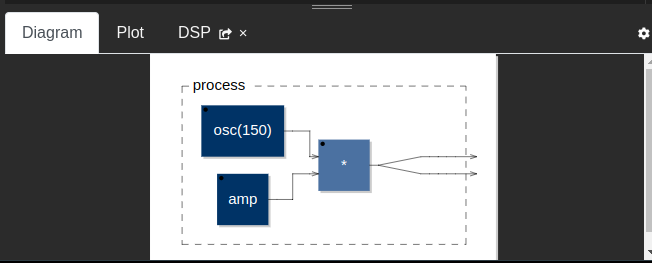
\includegraphics[width=0.8 \textwidth]{img/faust_diag.png}
	\caption{Block Diagramm in \texttt{FAUST}}
	\label{fig:faustBlock}
\end{figure}

Geneigten LeserInnen sei besonders empfohlen auch auf den 'Diagramm' button zu clicken um ein Blockdiagramm zu sehen dass dem Code/dem jeweiligen Konzept Entspricht.

Es kann nicht garantiert werden dass dieses Online-Service ständig online ist und die Details der Programmiersprache \texttt{FAUST} sind \textbf{nicht} Teil des Kurses.

\section*{Contributors}
Hier finden sich hoffentlich bald Menschen die diesen Text gelesen haben und Verbesserungsvorschläge gemacht haben.
\begin{itemize}
	\item Youjin Kim, Korrektur hinweis, Fehler in Aufgabe 1.6.
\end{itemize}

% \section*{General TODOs}
% \begin{itemize}
% 	% \item indexing
% 	\item proof reading..
% 	% \item Page numbers
% 	% \item scheinbar wird derzeit teilweise Text 'verschluckt'. zb linearfaktorzerlegung.
% \end{itemize}

\part{Semester I}
%!TEX root = main.tex
\chapter{Grundlagen}

\section{Motivation}

\todo[inline]{TODO, Dimensionsanalyse?}

\section{Aussagen}


% \begin{tcolorbox}[sidebarmark={Lecture 1}]



\begin{table}[h!]
    \centering
    \renewcommand{\arraystretch}{1.5} % Vergrößert den Zeilenabstand
    \begin{tabular}{|c|c|c|}
        \hline
        \textbf{Operation} & \textbf{Mathematische Notation} & \textbf{Erklärung} \\
        \hline
        Negation & $\neg A$ oder $\bar A$  & nicht A \\
        \hline
        Konjunktion & $A \land B$ & A und B \\
        \hline
        Disjunktion & $A \lor B$ & A oder B \\
        \hline
        Implikation & $A \implies B$ & Wenn A, dann B \\
        \hline
        Äquivalenz & $A \iff B$ & A genau dann, wenn B \\
        \hline
        Tautologie & $\top$ & immer wahr \\
        \hline
        Kontradiktion & $\bot$ & immer falsch \\
        \hline
    \end{tabular}
    \caption{Tabelle über mathematische Aussagen und Operationen}
\end{table}


\subsection{Quantoren}
\index{Quantor}
\begin{itemize}
    \item $\forall$, 'Allquantor'
    \item $\exists$, 'Existenzquantor'
\end{itemize}

\example{\textbf{Beispiel} \\
$\forall x \in X, \: A(x)$ : Für alle $x$ in $X$ ist die Aussage $A(x)$ wahr.

}

\subsection{Boolsche Logik}
\label{sec:bool}

\begin{table}[h!]
    \centering
    \begin{tabular}{|c|c|c|c|}
        \hline
        $A$ & $B$ & $A \land B$ & $A \lor B$ \\
        \hline
        0 & 0 & 0 & 0 \\
        0 & 1 & 0 & 1 \\
        1 & 0 & 0 & 1 \\
        1 & 1 & 1 & 1 \\
        \hline
    \end{tabular}
    \caption{Boolesche Algebra: UND und ODER Operationen}
\end{table}

\begin{table}[h!]
    \centering
    \begin{tabular}{|c|c|}
        \hline
        $A$ & $\neg A$ \\
        \hline
        0 & 1 \\
        1 & 0 \\
        \hline
    \end{tabular}
    \caption{Boolesche Algebra: NICHT Operation}
\end{table}

\praxis{Boolsche Logik: Programmieren}

\section{Mengen}
\index{Menge}
\important{Eine Menge ist eine Zusammenfassung unterscheidbarer Objekte zu einer Gesamtheit. Die Objekte werden 'Elemente' genannt}

% \equation{ 
Beispiele für \emph{explizite} Mengen:
$$ A = \{ \text{bla}, \text{franz}, \text{hubert} \} $$ 
$$ B = \{ 1, 3, 5, 8 \} $$ 

Beispiel für Mengen durch \emph{Beschreibung}:

$$ C = \{x \, | \, x \, \text{ist eine Geige} \} $$

Die Menge \emph{aller} Geigen.

\subsection{Operationen}

Vergl. mit Abschnitt \ref{sec:bool}!

\begin{itemize}
    \item \textbf{Durchschnitt} $ A \cap B = \{x \, | \, x \in A \land x \in B\}$
    \item \textbf{Vereinigung} $ A \cup B = \{x \, | \, x \in A \lor x \in B\}$
    \item \textbf{Differenz} $ A \setminus B = \{x \, | \, x \in A \land x \notin B\}$
\end{itemize}


\begin{figure}[h]
    \centering
    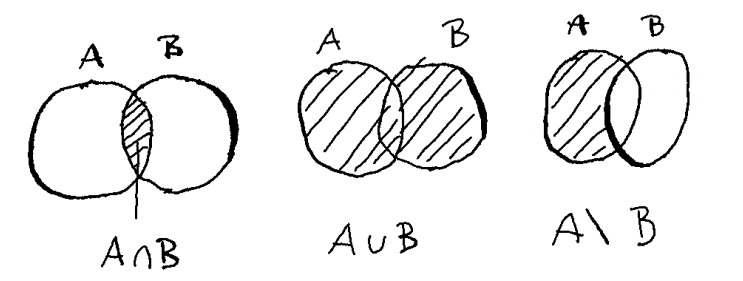
\includegraphics[width=0.5\textwidth]{img/mengenVenn.png}
    \caption{Venn Diagramme der Operationen auf Mengen $A$ und $B$.}
    \label{fig:vennMengen}
\end{figure}



\begin{figure}[h]
    \centering
    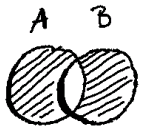
\includegraphics[width=0.1\textwidth]{img/mengen_symDiff.png}
    \caption{Symmetrische Differenz der Mengen $A$ und $B$.}
    \label{fig:venn_symDiff}
\end{figure}

\begin{question}
    Konstruiere die Situation in Abbildung \ref{fig:venn_symDiff}.
\end{question}

\begin{answer}
      $(A \cup B) \setminus (A \cap B)$. Siehe Abbildung \ref{fig:symDifSteps}.
\end{answer}

      \begin{figure}[h]
          \centering
          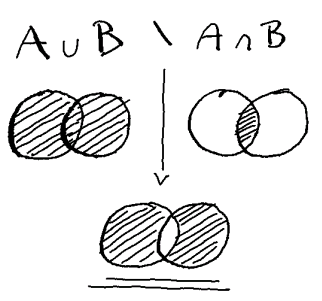
\includegraphics[width=0.2\textwidth]{img/symDifSteps.png}
          \caption{\emph{Symmetrische Differenz} in einzelnen Schritten veranschaulicht.}
          \label{fig:symDifSteps}
      \end{figure}


\subsection{Beschreibung von Teilmengen}
\begin{itemize}
    \item $A\subseteq B$. $A$ ist eine \textbf{Teilmenge} von $B$. Das heißt: $x \in A \implies x \in B$.
    \item $A\subset B$. $A$ ist eine \textbf{Echte Teilmenge} von $B$. Das heißt: $A\subseteq B \land A \neq B $.
\end{itemize}


\section{Funktionen, Abbildungen}
\label{sec:funktionen}

\todo[]{alles.}
Die \emph{Abbildung} oder \emph{Funktion} $f$ bildet die Menge $D$ auf die Menge $Z$ ab. Sie ordnet jedem Element von $D$ \emph{genau ein} Element von $Z$ zu.

    $$ f : D \to Z$$

Man schreibt $f\coloneqq x \mapsto y$ oder $f(x) = y$.

\begin{itemize}
    \item $D$ Definitionsbereich, Definitionsmenge
    \item $Z$ Zielmenge
    \item $f(A)$ Bildmenge (wobei stets $f(A)=B, B \in Z$, heißt: Die Bildmenge ist eine Teilmenge der Zielmenge.)
    \item $x$ unabhängige Variable
    \item $y$ abhängige Variable
    \item $f(x) = y$ Funktionsgleichung
\end{itemize}


\example{
    \textbf{Beispiel} \\
    $$f : \mathbb{R} \to \mathbb{R} , \: f(x) = sin(x)$$

    \begin{figure}[H]
        \centering
        %% Creator: Matplotlib, PGF backend
%%
%% To include the figure in your LaTeX document, write
%%   \input{<filename>.pgf}
%%
%% Make sure the required packages are loaded in your preamble
%%   \usepackage{pgf}
%%
%% Also ensure that all the required font packages are loaded; for instance,
%% the lmodern package is sometimes necessary when using math font.
%%   \usepackage{lmodern}
%%
%% Figures using additional raster images can only be included by \input if
%% they are in the same directory as the main LaTeX file. For loading figures
%% from other directories you can use the `import` package
%%   \usepackage{import}
%%
%% and then include the figures with
%%   \import{<path to file>}{<filename>.pgf}
%%
%% Matplotlib used the following preamble
%%   \def\mathdefault#1{#1}
%%   \everymath=\expandafter{\the\everymath\displaystyle}
%%   
%%   \usepackage{fontspec}
%%   \setmainfont{VeraSe.ttf}[Path=\detokenize{/usr/share/fonts/TTF/}]
%%   \setsansfont{DejaVuSans.ttf}[Path=\detokenize{/home/pl/miniconda3/lib/python3.12/site-packages/matplotlib/mpl-data/fonts/ttf/}]
%%   \setmonofont{DejaVuSansMono.ttf}[Path=\detokenize{/home/pl/miniconda3/lib/python3.12/site-packages/matplotlib/mpl-data/fonts/ttf/}]
%%   \makeatletter\@ifpackageloaded{underscore}{}{\usepackage[strings]{underscore}}\makeatother
%%
\begingroup%
\makeatletter%
\begin{pgfpicture}%
\pgfpathrectangle{\pgfpointorigin}{\pgfqpoint{2.956614in}{2.188486in}}%
\pgfusepath{use as bounding box, clip}%
\begin{pgfscope}%
\pgfsetbuttcap%
\pgfsetmiterjoin%
\definecolor{currentfill}{rgb}{1.000000,1.000000,1.000000}%
\pgfsetfillcolor{currentfill}%
\pgfsetlinewidth{0.000000pt}%
\definecolor{currentstroke}{rgb}{1.000000,1.000000,1.000000}%
\pgfsetstrokecolor{currentstroke}%
\pgfsetdash{}{0pt}%
\pgfpathmoveto{\pgfqpoint{0.000000in}{0.000000in}}%
\pgfpathlineto{\pgfqpoint{2.956614in}{0.000000in}}%
\pgfpathlineto{\pgfqpoint{2.956614in}{2.188486in}}%
\pgfpathlineto{\pgfqpoint{0.000000in}{2.188486in}}%
\pgfpathlineto{\pgfqpoint{0.000000in}{0.000000in}}%
\pgfpathclose%
\pgfusepath{fill}%
\end{pgfscope}%
\begin{pgfscope}%
\pgfsetbuttcap%
\pgfsetmiterjoin%
\definecolor{currentfill}{rgb}{1.000000,1.000000,1.000000}%
\pgfsetfillcolor{currentfill}%
\pgfsetlinewidth{0.000000pt}%
\definecolor{currentstroke}{rgb}{0.000000,0.000000,0.000000}%
\pgfsetstrokecolor{currentstroke}%
\pgfsetstrokeopacity{0.000000}%
\pgfsetdash{}{0pt}%
\pgfpathmoveto{\pgfqpoint{0.742978in}{0.548486in}}%
\pgfpathlineto{\pgfqpoint{2.856614in}{0.548486in}}%
\pgfpathlineto{\pgfqpoint{2.856614in}{2.088486in}}%
\pgfpathlineto{\pgfqpoint{0.742978in}{2.088486in}}%
\pgfpathlineto{\pgfqpoint{0.742978in}{0.548486in}}%
\pgfpathclose%
\pgfusepath{fill}%
\end{pgfscope}%
\begin{pgfscope}%
\pgfsetbuttcap%
\pgfsetroundjoin%
\definecolor{currentfill}{rgb}{0.000000,0.000000,0.000000}%
\pgfsetfillcolor{currentfill}%
\pgfsetlinewidth{0.803000pt}%
\definecolor{currentstroke}{rgb}{0.000000,0.000000,0.000000}%
\pgfsetstrokecolor{currentstroke}%
\pgfsetdash{}{0pt}%
\pgfsys@defobject{currentmarker}{\pgfqpoint{0.000000in}{-0.048611in}}{\pgfqpoint{0.000000in}{0.000000in}}{%
\pgfpathmoveto{\pgfqpoint{0.000000in}{0.000000in}}%
\pgfpathlineto{\pgfqpoint{0.000000in}{-0.048611in}}%
\pgfusepath{stroke,fill}%
}%
\begin{pgfscope}%
\pgfsys@transformshift{1.035260in}{0.548486in}%
\pgfsys@useobject{currentmarker}{}%
\end{pgfscope}%
\end{pgfscope}%
\begin{pgfscope}%
\definecolor{textcolor}{rgb}{0.000000,0.000000,0.000000}%
\pgfsetstrokecolor{textcolor}%
\pgfsetfillcolor{textcolor}%
\pgftext[x=1.035260in,y=0.451264in,,top]{\color{textcolor}{\rmfamily\fontsize{10.000000}{12.000000}\selectfont\catcode`\^=\active\def^{\ifmmode\sp\else\^{}\fi}\catcode`\%=\active\def%{\%}\ensuremath{-}5}}%
\end{pgfscope}%
\begin{pgfscope}%
\pgfsetbuttcap%
\pgfsetroundjoin%
\definecolor{currentfill}{rgb}{0.000000,0.000000,0.000000}%
\pgfsetfillcolor{currentfill}%
\pgfsetlinewidth{0.803000pt}%
\definecolor{currentstroke}{rgb}{0.000000,0.000000,0.000000}%
\pgfsetstrokecolor{currentstroke}%
\pgfsetdash{}{0pt}%
\pgfsys@defobject{currentmarker}{\pgfqpoint{0.000000in}{-0.048611in}}{\pgfqpoint{0.000000in}{0.000000in}}{%
\pgfpathmoveto{\pgfqpoint{0.000000in}{0.000000in}}%
\pgfpathlineto{\pgfqpoint{0.000000in}{-0.048611in}}%
\pgfusepath{stroke,fill}%
}%
\begin{pgfscope}%
\pgfsys@transformshift{1.799796in}{0.548486in}%
\pgfsys@useobject{currentmarker}{}%
\end{pgfscope}%
\end{pgfscope}%
\begin{pgfscope}%
\definecolor{textcolor}{rgb}{0.000000,0.000000,0.000000}%
\pgfsetstrokecolor{textcolor}%
\pgfsetfillcolor{textcolor}%
\pgftext[x=1.799796in,y=0.451264in,,top]{\color{textcolor}{\rmfamily\fontsize{10.000000}{12.000000}\selectfont\catcode`\^=\active\def^{\ifmmode\sp\else\^{}\fi}\catcode`\%=\active\def%{\%}0}}%
\end{pgfscope}%
\begin{pgfscope}%
\pgfsetbuttcap%
\pgfsetroundjoin%
\definecolor{currentfill}{rgb}{0.000000,0.000000,0.000000}%
\pgfsetfillcolor{currentfill}%
\pgfsetlinewidth{0.803000pt}%
\definecolor{currentstroke}{rgb}{0.000000,0.000000,0.000000}%
\pgfsetstrokecolor{currentstroke}%
\pgfsetdash{}{0pt}%
\pgfsys@defobject{currentmarker}{\pgfqpoint{0.000000in}{-0.048611in}}{\pgfqpoint{0.000000in}{0.000000in}}{%
\pgfpathmoveto{\pgfqpoint{0.000000in}{0.000000in}}%
\pgfpathlineto{\pgfqpoint{0.000000in}{-0.048611in}}%
\pgfusepath{stroke,fill}%
}%
\begin{pgfscope}%
\pgfsys@transformshift{2.564331in}{0.548486in}%
\pgfsys@useobject{currentmarker}{}%
\end{pgfscope}%
\end{pgfscope}%
\begin{pgfscope}%
\definecolor{textcolor}{rgb}{0.000000,0.000000,0.000000}%
\pgfsetstrokecolor{textcolor}%
\pgfsetfillcolor{textcolor}%
\pgftext[x=2.564331in,y=0.451264in,,top]{\color{textcolor}{\rmfamily\fontsize{10.000000}{12.000000}\selectfont\catcode`\^=\active\def^{\ifmmode\sp\else\^{}\fi}\catcode`\%=\active\def%{\%}5}}%
\end{pgfscope}%
\begin{pgfscope}%
\definecolor{textcolor}{rgb}{0.000000,0.000000,0.000000}%
\pgfsetstrokecolor{textcolor}%
\pgfsetfillcolor{textcolor}%
\pgftext[x=1.799796in,y=0.261295in,,top]{\color{textcolor}{\rmfamily\fontsize{12.000000}{14.400000}\selectfont\catcode`\^=\active\def^{\ifmmode\sp\else\^{}\fi}\catcode`\%=\active\def%{\%}$x$}}%
\end{pgfscope}%
\begin{pgfscope}%
\pgfsetbuttcap%
\pgfsetroundjoin%
\definecolor{currentfill}{rgb}{0.000000,0.000000,0.000000}%
\pgfsetfillcolor{currentfill}%
\pgfsetlinewidth{0.803000pt}%
\definecolor{currentstroke}{rgb}{0.000000,0.000000,0.000000}%
\pgfsetstrokecolor{currentstroke}%
\pgfsetdash{}{0pt}%
\pgfsys@defobject{currentmarker}{\pgfqpoint{-0.048611in}{0.000000in}}{\pgfqpoint{-0.000000in}{0.000000in}}{%
\pgfpathmoveto{\pgfqpoint{-0.000000in}{0.000000in}}%
\pgfpathlineto{\pgfqpoint{-0.048611in}{0.000000in}}%
\pgfusepath{stroke,fill}%
}%
\begin{pgfscope}%
\pgfsys@transformshift{0.742978in}{0.676819in}%
\pgfsys@useobject{currentmarker}{}%
\end{pgfscope}%
\end{pgfscope}%
\begin{pgfscope}%
\definecolor{textcolor}{rgb}{0.000000,0.000000,0.000000}%
\pgfsetstrokecolor{textcolor}%
\pgfsetfillcolor{textcolor}%
\pgftext[x=0.316851in, y=0.624058in, left, base]{\color{textcolor}{\rmfamily\fontsize{10.000000}{12.000000}\selectfont\catcode`\^=\active\def^{\ifmmode\sp\else\^{}\fi}\catcode`\%=\active\def%{\%}\ensuremath{-}1.0}}%
\end{pgfscope}%
\begin{pgfscope}%
\pgfsetbuttcap%
\pgfsetroundjoin%
\definecolor{currentfill}{rgb}{0.000000,0.000000,0.000000}%
\pgfsetfillcolor{currentfill}%
\pgfsetlinewidth{0.803000pt}%
\definecolor{currentstroke}{rgb}{0.000000,0.000000,0.000000}%
\pgfsetstrokecolor{currentstroke}%
\pgfsetdash{}{0pt}%
\pgfsys@defobject{currentmarker}{\pgfqpoint{-0.048611in}{0.000000in}}{\pgfqpoint{-0.000000in}{0.000000in}}{%
\pgfpathmoveto{\pgfqpoint{-0.000000in}{0.000000in}}%
\pgfpathlineto{\pgfqpoint{-0.048611in}{0.000000in}}%
\pgfusepath{stroke,fill}%
}%
\begin{pgfscope}%
\pgfsys@transformshift{0.742978in}{0.997653in}%
\pgfsys@useobject{currentmarker}{}%
\end{pgfscope}%
\end{pgfscope}%
\begin{pgfscope}%
\definecolor{textcolor}{rgb}{0.000000,0.000000,0.000000}%
\pgfsetstrokecolor{textcolor}%
\pgfsetfillcolor{textcolor}%
\pgftext[x=0.316851in, y=0.944891in, left, base]{\color{textcolor}{\rmfamily\fontsize{10.000000}{12.000000}\selectfont\catcode`\^=\active\def^{\ifmmode\sp\else\^{}\fi}\catcode`\%=\active\def%{\%}\ensuremath{-}0.5}}%
\end{pgfscope}%
\begin{pgfscope}%
\pgfsetbuttcap%
\pgfsetroundjoin%
\definecolor{currentfill}{rgb}{0.000000,0.000000,0.000000}%
\pgfsetfillcolor{currentfill}%
\pgfsetlinewidth{0.803000pt}%
\definecolor{currentstroke}{rgb}{0.000000,0.000000,0.000000}%
\pgfsetstrokecolor{currentstroke}%
\pgfsetdash{}{0pt}%
\pgfsys@defobject{currentmarker}{\pgfqpoint{-0.048611in}{0.000000in}}{\pgfqpoint{-0.000000in}{0.000000in}}{%
\pgfpathmoveto{\pgfqpoint{-0.000000in}{0.000000in}}%
\pgfpathlineto{\pgfqpoint{-0.048611in}{0.000000in}}%
\pgfusepath{stroke,fill}%
}%
\begin{pgfscope}%
\pgfsys@transformshift{0.742978in}{1.318486in}%
\pgfsys@useobject{currentmarker}{}%
\end{pgfscope}%
\end{pgfscope}%
\begin{pgfscope}%
\definecolor{textcolor}{rgb}{0.000000,0.000000,0.000000}%
\pgfsetstrokecolor{textcolor}%
\pgfsetfillcolor{textcolor}%
\pgftext[x=0.424876in, y=1.265724in, left, base]{\color{textcolor}{\rmfamily\fontsize{10.000000}{12.000000}\selectfont\catcode`\^=\active\def^{\ifmmode\sp\else\^{}\fi}\catcode`\%=\active\def%{\%}0.0}}%
\end{pgfscope}%
\begin{pgfscope}%
\pgfsetbuttcap%
\pgfsetroundjoin%
\definecolor{currentfill}{rgb}{0.000000,0.000000,0.000000}%
\pgfsetfillcolor{currentfill}%
\pgfsetlinewidth{0.803000pt}%
\definecolor{currentstroke}{rgb}{0.000000,0.000000,0.000000}%
\pgfsetstrokecolor{currentstroke}%
\pgfsetdash{}{0pt}%
\pgfsys@defobject{currentmarker}{\pgfqpoint{-0.048611in}{0.000000in}}{\pgfqpoint{-0.000000in}{0.000000in}}{%
\pgfpathmoveto{\pgfqpoint{-0.000000in}{0.000000in}}%
\pgfpathlineto{\pgfqpoint{-0.048611in}{0.000000in}}%
\pgfusepath{stroke,fill}%
}%
\begin{pgfscope}%
\pgfsys@transformshift{0.742978in}{1.639319in}%
\pgfsys@useobject{currentmarker}{}%
\end{pgfscope}%
\end{pgfscope}%
\begin{pgfscope}%
\definecolor{textcolor}{rgb}{0.000000,0.000000,0.000000}%
\pgfsetstrokecolor{textcolor}%
\pgfsetfillcolor{textcolor}%
\pgftext[x=0.424876in, y=1.586558in, left, base]{\color{textcolor}{\rmfamily\fontsize{10.000000}{12.000000}\selectfont\catcode`\^=\active\def^{\ifmmode\sp\else\^{}\fi}\catcode`\%=\active\def%{\%}0.5}}%
\end{pgfscope}%
\begin{pgfscope}%
\pgfsetbuttcap%
\pgfsetroundjoin%
\definecolor{currentfill}{rgb}{0.000000,0.000000,0.000000}%
\pgfsetfillcolor{currentfill}%
\pgfsetlinewidth{0.803000pt}%
\definecolor{currentstroke}{rgb}{0.000000,0.000000,0.000000}%
\pgfsetstrokecolor{currentstroke}%
\pgfsetdash{}{0pt}%
\pgfsys@defobject{currentmarker}{\pgfqpoint{-0.048611in}{0.000000in}}{\pgfqpoint{-0.000000in}{0.000000in}}{%
\pgfpathmoveto{\pgfqpoint{-0.000000in}{0.000000in}}%
\pgfpathlineto{\pgfqpoint{-0.048611in}{0.000000in}}%
\pgfusepath{stroke,fill}%
}%
\begin{pgfscope}%
\pgfsys@transformshift{0.742978in}{1.960153in}%
\pgfsys@useobject{currentmarker}{}%
\end{pgfscope}%
\end{pgfscope}%
\begin{pgfscope}%
\definecolor{textcolor}{rgb}{0.000000,0.000000,0.000000}%
\pgfsetstrokecolor{textcolor}%
\pgfsetfillcolor{textcolor}%
\pgftext[x=0.424876in, y=1.907391in, left, base]{\color{textcolor}{\rmfamily\fontsize{10.000000}{12.000000}\selectfont\catcode`\^=\active\def^{\ifmmode\sp\else\^{}\fi}\catcode`\%=\active\def%{\%}1.0}}%
\end{pgfscope}%
\begin{pgfscope}%
\definecolor{textcolor}{rgb}{0.000000,0.000000,0.000000}%
\pgfsetstrokecolor{textcolor}%
\pgfsetfillcolor{textcolor}%
\pgftext[x=0.261295in,y=1.318486in,,bottom,rotate=90.000000]{\color{textcolor}{\rmfamily\fontsize{12.000000}{14.400000}\selectfont\catcode`\^=\active\def^{\ifmmode\sp\else\^{}\fi}\catcode`\%=\active\def%{\%}$y$}}%
\end{pgfscope}%
\begin{pgfscope}%
\pgfpathrectangle{\pgfqpoint{0.742978in}{0.548486in}}{\pgfqpoint{2.113636in}{1.540000in}}%
\pgfusepath{clip}%
\pgfsetrectcap%
\pgfsetroundjoin%
\pgfsetlinewidth{1.505625pt}%
\definecolor{currentstroke}{rgb}{0.000000,0.000000,0.000000}%
\pgfsetstrokecolor{currentstroke}%
\pgfsetdash{}{0pt}%
\pgfpathmoveto{\pgfqpoint{0.839052in}{1.318486in}}%
\pgfpathlineto{\pgfqpoint{0.858461in}{1.399716in}}%
\pgfpathlineto{\pgfqpoint{0.877870in}{1.479639in}}%
\pgfpathlineto{\pgfqpoint{0.897279in}{1.556969in}}%
\pgfpathlineto{\pgfqpoint{0.916688in}{1.630462in}}%
\pgfpathlineto{\pgfqpoint{0.936097in}{1.698935in}}%
\pgfpathlineto{\pgfqpoint{0.955506in}{1.761287in}}%
\pgfpathlineto{\pgfqpoint{0.974915in}{1.816513in}}%
\pgfpathlineto{\pgfqpoint{0.994324in}{1.863726in}}%
\pgfpathlineto{\pgfqpoint{1.013733in}{1.902167in}}%
\pgfpathlineto{\pgfqpoint{1.033142in}{1.931215in}}%
\pgfpathlineto{\pgfqpoint{1.052551in}{1.950404in}}%
\pgfpathlineto{\pgfqpoint{1.071960in}{1.959426in}}%
\pgfpathlineto{\pgfqpoint{1.091369in}{1.958134in}}%
\pgfpathlineto{\pgfqpoint{1.110778in}{1.946551in}}%
\pgfpathlineto{\pgfqpoint{1.130187in}{1.924861in}}%
\pgfpathlineto{\pgfqpoint{1.149595in}{1.893415in}}%
\pgfpathlineto{\pgfqpoint{1.169004in}{1.852718in}}%
\pgfpathlineto{\pgfqpoint{1.188413in}{1.803425in}}%
\pgfpathlineto{\pgfqpoint{1.207822in}{1.746329in}}%
\pgfpathlineto{\pgfqpoint{1.227231in}{1.682349in}}%
\pgfpathlineto{\pgfqpoint{1.246640in}{1.612515in}}%
\pgfpathlineto{\pgfqpoint{1.266049in}{1.537949in}}%
\pgfpathlineto{\pgfqpoint{1.285458in}{1.459852in}}%
\pgfpathlineto{\pgfqpoint{1.304867in}{1.379480in}}%
\pgfpathlineto{\pgfqpoint{1.324276in}{1.298127in}}%
\pgfpathlineto{\pgfqpoint{1.343685in}{1.217102in}}%
\pgfpathlineto{\pgfqpoint{1.363094in}{1.137708in}}%
\pgfpathlineto{\pgfqpoint{1.382503in}{1.061222in}}%
\pgfpathlineto{\pgfqpoint{1.401912in}{0.988876in}}%
\pgfpathlineto{\pgfqpoint{1.421321in}{0.921834in}}%
\pgfpathlineto{\pgfqpoint{1.440730in}{0.861174in}}%
\pgfpathlineto{\pgfqpoint{1.460139in}{0.807872in}}%
\pgfpathlineto{\pgfqpoint{1.479548in}{0.762786in}}%
\pgfpathlineto{\pgfqpoint{1.498957in}{0.726642in}}%
\pgfpathlineto{\pgfqpoint{1.518366in}{0.700021in}}%
\pgfpathlineto{\pgfqpoint{1.537775in}{0.683351in}}%
\pgfpathlineto{\pgfqpoint{1.557184in}{0.676900in}}%
\pgfpathlineto{\pgfqpoint{1.576593in}{0.680773in}}%
\pgfpathlineto{\pgfqpoint{1.596002in}{0.694907in}}%
\pgfpathlineto{\pgfqpoint{1.615411in}{0.719074in}}%
\pgfpathlineto{\pgfqpoint{1.634820in}{0.752887in}}%
\pgfpathlineto{\pgfqpoint{1.654229in}{0.795800in}}%
\pgfpathlineto{\pgfqpoint{1.673638in}{0.847123in}}%
\pgfpathlineto{\pgfqpoint{1.693047in}{0.906031in}}%
\pgfpathlineto{\pgfqpoint{1.712455in}{0.971575in}}%
\pgfpathlineto{\pgfqpoint{1.731864in}{1.042701in}}%
\pgfpathlineto{\pgfqpoint{1.751273in}{1.118265in}}%
\pgfpathlineto{\pgfqpoint{1.770682in}{1.197050in}}%
\pgfpathlineto{\pgfqpoint{1.790091in}{1.277789in}}%
\pgfpathlineto{\pgfqpoint{1.809500in}{1.359183in}}%
\pgfpathlineto{\pgfqpoint{1.828909in}{1.439922in}}%
\pgfpathlineto{\pgfqpoint{1.848318in}{1.518707in}}%
\pgfpathlineto{\pgfqpoint{1.867727in}{1.594271in}}%
\pgfpathlineto{\pgfqpoint{1.887136in}{1.665397in}}%
\pgfpathlineto{\pgfqpoint{1.906545in}{1.730941in}}%
\pgfpathlineto{\pgfqpoint{1.925954in}{1.789849in}}%
\pgfpathlineto{\pgfqpoint{1.945363in}{1.841172in}}%
\pgfpathlineto{\pgfqpoint{1.964772in}{1.884085in}}%
\pgfpathlineto{\pgfqpoint{1.984181in}{1.917898in}}%
\pgfpathlineto{\pgfqpoint{2.003590in}{1.942065in}}%
\pgfpathlineto{\pgfqpoint{2.022999in}{1.956199in}}%
\pgfpathlineto{\pgfqpoint{2.042408in}{1.960072in}}%
\pgfpathlineto{\pgfqpoint{2.061817in}{1.953621in}}%
\pgfpathlineto{\pgfqpoint{2.081226in}{1.936951in}}%
\pgfpathlineto{\pgfqpoint{2.100635in}{1.910330in}}%
\pgfpathlineto{\pgfqpoint{2.120044in}{1.874186in}}%
\pgfpathlineto{\pgfqpoint{2.139453in}{1.829100in}}%
\pgfpathlineto{\pgfqpoint{2.158862in}{1.775798in}}%
\pgfpathlineto{\pgfqpoint{2.178271in}{1.715138in}}%
\pgfpathlineto{\pgfqpoint{2.197680in}{1.648096in}}%
\pgfpathlineto{\pgfqpoint{2.217089in}{1.575750in}}%
\pgfpathlineto{\pgfqpoint{2.236498in}{1.499264in}}%
\pgfpathlineto{\pgfqpoint{2.255907in}{1.419870in}}%
\pgfpathlineto{\pgfqpoint{2.275315in}{1.338845in}}%
\pgfpathlineto{\pgfqpoint{2.294724in}{1.257492in}}%
\pgfpathlineto{\pgfqpoint{2.314133in}{1.177120in}}%
\pgfpathlineto{\pgfqpoint{2.333542in}{1.099023in}}%
\pgfpathlineto{\pgfqpoint{2.352951in}{1.024457in}}%
\pgfpathlineto{\pgfqpoint{2.372360in}{0.954623in}}%
\pgfpathlineto{\pgfqpoint{2.391769in}{0.890643in}}%
\pgfpathlineto{\pgfqpoint{2.411178in}{0.833547in}}%
\pgfpathlineto{\pgfqpoint{2.430587in}{0.784254in}}%
\pgfpathlineto{\pgfqpoint{2.449996in}{0.743557in}}%
\pgfpathlineto{\pgfqpoint{2.469405in}{0.712110in}}%
\pgfpathlineto{\pgfqpoint{2.488814in}{0.690421in}}%
\pgfpathlineto{\pgfqpoint{2.508223in}{0.678837in}}%
\pgfpathlineto{\pgfqpoint{2.527632in}{0.677546in}}%
\pgfpathlineto{\pgfqpoint{2.547041in}{0.686568in}}%
\pgfpathlineto{\pgfqpoint{2.566450in}{0.705757in}}%
\pgfpathlineto{\pgfqpoint{2.585859in}{0.734805in}}%
\pgfpathlineto{\pgfqpoint{2.605268in}{0.773245in}}%
\pgfpathlineto{\pgfqpoint{2.624677in}{0.820459in}}%
\pgfpathlineto{\pgfqpoint{2.644086in}{0.875685in}}%
\pgfpathlineto{\pgfqpoint{2.663495in}{0.938037in}}%
\pgfpathlineto{\pgfqpoint{2.682904in}{1.006510in}}%
\pgfpathlineto{\pgfqpoint{2.702313in}{1.080003in}}%
\pgfpathlineto{\pgfqpoint{2.721722in}{1.157333in}}%
\pgfpathlineto{\pgfqpoint{2.741131in}{1.237256in}}%
\pgfpathlineto{\pgfqpoint{2.760540in}{1.318486in}}%
\pgfusepath{stroke}%
\end{pgfscope}%
\begin{pgfscope}%
\pgfpathrectangle{\pgfqpoint{0.742978in}{0.548486in}}{\pgfqpoint{2.113636in}{1.540000in}}%
\pgfusepath{clip}%
\pgfsetrectcap%
\pgfsetroundjoin%
\pgfsetlinewidth{0.501875pt}%
\definecolor{currentstroke}{rgb}{0.000000,0.000000,0.000000}%
\pgfsetstrokecolor{currentstroke}%
\pgfsetdash{}{0pt}%
\pgfpathmoveto{\pgfqpoint{0.742978in}{1.318486in}}%
\pgfpathlineto{\pgfqpoint{2.856614in}{1.318486in}}%
\pgfusepath{stroke}%
\end{pgfscope}%
\begin{pgfscope}%
\pgfpathrectangle{\pgfqpoint{0.742978in}{0.548486in}}{\pgfqpoint{2.113636in}{1.540000in}}%
\pgfusepath{clip}%
\pgfsetrectcap%
\pgfsetroundjoin%
\pgfsetlinewidth{0.501875pt}%
\definecolor{currentstroke}{rgb}{0.000000,0.000000,0.000000}%
\pgfsetstrokecolor{currentstroke}%
\pgfsetdash{}{0pt}%
\pgfpathmoveto{\pgfqpoint{1.799796in}{0.548486in}}%
\pgfpathlineto{\pgfqpoint{1.799796in}{2.088486in}}%
\pgfusepath{stroke}%
\end{pgfscope}%
\begin{pgfscope}%
\pgfsetbuttcap%
\pgfsetmiterjoin%
\definecolor{currentfill}{rgb}{1.000000,1.000000,1.000000}%
\pgfsetfillcolor{currentfill}%
\pgfsetfillopacity{0.800000}%
\pgfsetlinewidth{1.003750pt}%
\definecolor{currentstroke}{rgb}{0.800000,0.800000,0.800000}%
\pgfsetstrokecolor{currentstroke}%
\pgfsetstrokeopacity{0.800000}%
\pgfsetdash{}{0pt}%
\pgfpathmoveto{\pgfqpoint{2.044596in}{1.767685in}}%
\pgfpathlineto{\pgfqpoint{2.759392in}{1.767685in}}%
\pgfpathquadraticcurveto{\pgfqpoint{2.787170in}{1.767685in}}{\pgfqpoint{2.787170in}{1.795463in}}%
\pgfpathlineto{\pgfqpoint{2.787170in}{1.991264in}}%
\pgfpathquadraticcurveto{\pgfqpoint{2.787170in}{2.019042in}}{\pgfqpoint{2.759392in}{2.019042in}}%
\pgfpathlineto{\pgfqpoint{2.044596in}{2.019042in}}%
\pgfpathquadraticcurveto{\pgfqpoint{2.016818in}{2.019042in}}{\pgfqpoint{2.016818in}{1.991264in}}%
\pgfpathlineto{\pgfqpoint{2.016818in}{1.795463in}}%
\pgfpathquadraticcurveto{\pgfqpoint{2.016818in}{1.767685in}}{\pgfqpoint{2.044596in}{1.767685in}}%
\pgfpathlineto{\pgfqpoint{2.044596in}{1.767685in}}%
\pgfpathclose%
\pgfusepath{stroke,fill}%
\end{pgfscope}%
\begin{pgfscope}%
\pgfsetrectcap%
\pgfsetroundjoin%
\pgfsetlinewidth{1.505625pt}%
\definecolor{currentstroke}{rgb}{0.000000,0.000000,0.000000}%
\pgfsetstrokecolor{currentstroke}%
\pgfsetdash{}{0pt}%
\pgfpathmoveto{\pgfqpoint{2.072373in}{1.906574in}}%
\pgfpathlineto{\pgfqpoint{2.211262in}{1.906574in}}%
\pgfpathlineto{\pgfqpoint{2.350151in}{1.906574in}}%
\pgfusepath{stroke}%
\end{pgfscope}%
\begin{pgfscope}%
\definecolor{textcolor}{rgb}{0.000000,0.000000,0.000000}%
\pgfsetstrokecolor{textcolor}%
\pgfsetfillcolor{textcolor}%
\pgftext[x=2.461262in,y=1.857963in,left,base]{\color{textcolor}{\rmfamily\fontsize{10.000000}{12.000000}\selectfont\catcode`\^=\active\def^{\ifmmode\sp\else\^{}\fi}\catcode`\%=\active\def%{\%}$f(x)$}}%
\end{pgfscope}%
\end{pgfpicture}%
\makeatother%
\endgroup%

        % \includegraphics[]{}
        \caption{Der Funktionsgraph der Funktion $f(x)$.}
        \label{fig:figure1}
    \end{figure}
}

\subsection{Gerade und Ungerade Funktionen}\label{subsec:geradeUngerade}
Von \href{https://de.wikipedia.org/wiki/Gerade\_und\_ungerade\_Funktionen}{Wikipedia}, um zu demonstrieren dass das zuvor gelernte ständig anzutreffen ist:

\emph{'Eine reelle Funktion $f\colon D\to \mathbb {R} $ mit einer bezüglich der Null symmetrischen Definitionsmenge 
$ D\subseteq \mathbb {R}$ heißt gerade, wenn für alle Argumente $ x\in D$  $f(-x)=f(x)$.'} \\

Ungerade und Gerade Funktionen kurz zusammengefasst:
\begin{itemize}
    \item Gerade Funktion:  $f(-x) = f(x)$. Achsensymmetrisch zur $y$-Achse.
    \item Ungerade Funktion:  $f(-x) = -f(x)$. Punktsymmetrisch zum Ursprung.
\end{itemize}

    \begin{figure}[H]
        \centering
        %% Creator: Matplotlib, PGF backend
%%
%% To include the figure in your LaTeX document, write
%%   \input{<filename>.pgf}
%%
%% Make sure the required packages are loaded in your preamble
%%   \usepackage{pgf}
%%
%% Also ensure that all the required font packages are loaded; for instance,
%% the lmodern package is sometimes necessary when using math font.
%%   \usepackage{lmodern}
%%
%% Figures using additional raster images can only be included by \input if
%% they are in the same directory as the main LaTeX file. For loading figures
%% from other directories you can use the `import` package
%%   \usepackage{import}
%%
%% and then include the figures with
%%   \import{<path to file>}{<filename>.pgf}
%%
%% Matplotlib used the following preamble
%%   
%%   \usepackage{fontspec}
%%   \setmainfont{DejaVuSerif.ttf}[Path=\detokenize{/home/pl/anaconda3/lib/python3.11/site-packages/matplotlib/mpl-data/fonts/ttf/}]
%%   \setsansfont{DejaVuSans.ttf}[Path=\detokenize{/home/pl/anaconda3/lib/python3.11/site-packages/matplotlib/mpl-data/fonts/ttf/}]
%%   \setmonofont{DejaVuSansMono.ttf}[Path=\detokenize{/home/pl/anaconda3/lib/python3.11/site-packages/matplotlib/mpl-data/fonts/ttf/}]
%%   \makeatletter\@ifpackageloaded{underscore}{}{\usepackage[strings]{underscore}}\makeatother
%%
\begingroup%
\makeatletter%
\begin{pgfpicture}%
\pgfpathrectangle{\pgfpointorigin}{\pgfqpoint{5.347946in}{2.984365in}}%
\pgfusepath{use as bounding box, clip}%
\begin{pgfscope}%
\pgfsetbuttcap%
\pgfsetmiterjoin%
\definecolor{currentfill}{rgb}{1.000000,1.000000,1.000000}%
\pgfsetfillcolor{currentfill}%
\pgfsetlinewidth{0.000000pt}%
\definecolor{currentstroke}{rgb}{1.000000,1.000000,1.000000}%
\pgfsetstrokecolor{currentstroke}%
\pgfsetdash{}{0pt}%
\pgfpathmoveto{\pgfqpoint{0.000000in}{0.000000in}}%
\pgfpathlineto{\pgfqpoint{5.347946in}{0.000000in}}%
\pgfpathlineto{\pgfqpoint{5.347946in}{2.984365in}}%
\pgfpathlineto{\pgfqpoint{0.000000in}{2.984365in}}%
\pgfpathlineto{\pgfqpoint{0.000000in}{0.000000in}}%
\pgfpathclose%
\pgfusepath{fill}%
\end{pgfscope}%
\begin{pgfscope}%
\pgfsetbuttcap%
\pgfsetmiterjoin%
\definecolor{currentfill}{rgb}{1.000000,1.000000,1.000000}%
\pgfsetfillcolor{currentfill}%
\pgfsetlinewidth{0.000000pt}%
\definecolor{currentstroke}{rgb}{0.000000,0.000000,0.000000}%
\pgfsetstrokecolor{currentstroke}%
\pgfsetstrokeopacity{0.000000}%
\pgfsetdash{}{0pt}%
\pgfpathmoveto{\pgfqpoint{0.583581in}{0.521603in}}%
\pgfpathlineto{\pgfqpoint{2.697217in}{0.521603in}}%
\pgfpathlineto{\pgfqpoint{2.697217in}{2.831603in}}%
\pgfpathlineto{\pgfqpoint{0.583581in}{2.831603in}}%
\pgfpathlineto{\pgfqpoint{0.583581in}{0.521603in}}%
\pgfpathclose%
\pgfusepath{fill}%
\end{pgfscope}%
\begin{pgfscope}%
\pgfsetbuttcap%
\pgfsetroundjoin%
\definecolor{currentfill}{rgb}{0.000000,0.000000,0.000000}%
\pgfsetfillcolor{currentfill}%
\pgfsetlinewidth{0.803000pt}%
\definecolor{currentstroke}{rgb}{0.000000,0.000000,0.000000}%
\pgfsetstrokecolor{currentstroke}%
\pgfsetdash{}{0pt}%
\pgfsys@defobject{currentmarker}{\pgfqpoint{0.000000in}{-0.048611in}}{\pgfqpoint{0.000000in}{0.000000in}}{%
\pgfpathmoveto{\pgfqpoint{0.000000in}{0.000000in}}%
\pgfpathlineto{\pgfqpoint{0.000000in}{-0.048611in}}%
\pgfusepath{stroke,fill}%
}%
\begin{pgfscope}%
\pgfsys@transformshift{0.679655in}{0.521603in}%
\pgfsys@useobject{currentmarker}{}%
\end{pgfscope}%
\end{pgfscope}%
\begin{pgfscope}%
\definecolor{textcolor}{rgb}{0.000000,0.000000,0.000000}%
\pgfsetstrokecolor{textcolor}%
\pgfsetfillcolor{textcolor}%
\pgftext[x=0.679655in,y=0.424381in,,top]{\color{textcolor}\rmfamily\fontsize{10.000000}{12.000000}\selectfont \ensuremath{-}5.0}%
\end{pgfscope}%
\begin{pgfscope}%
\pgfsetbuttcap%
\pgfsetroundjoin%
\definecolor{currentfill}{rgb}{0.000000,0.000000,0.000000}%
\pgfsetfillcolor{currentfill}%
\pgfsetlinewidth{0.803000pt}%
\definecolor{currentstroke}{rgb}{0.000000,0.000000,0.000000}%
\pgfsetstrokecolor{currentstroke}%
\pgfsetdash{}{0pt}%
\pgfsys@defobject{currentmarker}{\pgfqpoint{0.000000in}{-0.048611in}}{\pgfqpoint{0.000000in}{0.000000in}}{%
\pgfpathmoveto{\pgfqpoint{0.000000in}{0.000000in}}%
\pgfpathlineto{\pgfqpoint{0.000000in}{-0.048611in}}%
\pgfusepath{stroke,fill}%
}%
\begin{pgfscope}%
\pgfsys@transformshift{1.160027in}{0.521603in}%
\pgfsys@useobject{currentmarker}{}%
\end{pgfscope}%
\end{pgfscope}%
\begin{pgfscope}%
\definecolor{textcolor}{rgb}{0.000000,0.000000,0.000000}%
\pgfsetstrokecolor{textcolor}%
\pgfsetfillcolor{textcolor}%
\pgftext[x=1.160027in,y=0.424381in,,top]{\color{textcolor}\rmfamily\fontsize{10.000000}{12.000000}\selectfont \ensuremath{-}2.5}%
\end{pgfscope}%
\begin{pgfscope}%
\pgfsetbuttcap%
\pgfsetroundjoin%
\definecolor{currentfill}{rgb}{0.000000,0.000000,0.000000}%
\pgfsetfillcolor{currentfill}%
\pgfsetlinewidth{0.803000pt}%
\definecolor{currentstroke}{rgb}{0.000000,0.000000,0.000000}%
\pgfsetstrokecolor{currentstroke}%
\pgfsetdash{}{0pt}%
\pgfsys@defobject{currentmarker}{\pgfqpoint{0.000000in}{-0.048611in}}{\pgfqpoint{0.000000in}{0.000000in}}{%
\pgfpathmoveto{\pgfqpoint{0.000000in}{0.000000in}}%
\pgfpathlineto{\pgfqpoint{0.000000in}{-0.048611in}}%
\pgfusepath{stroke,fill}%
}%
\begin{pgfscope}%
\pgfsys@transformshift{1.640399in}{0.521603in}%
\pgfsys@useobject{currentmarker}{}%
\end{pgfscope}%
\end{pgfscope}%
\begin{pgfscope}%
\definecolor{textcolor}{rgb}{0.000000,0.000000,0.000000}%
\pgfsetstrokecolor{textcolor}%
\pgfsetfillcolor{textcolor}%
\pgftext[x=1.640399in,y=0.424381in,,top]{\color{textcolor}\rmfamily\fontsize{10.000000}{12.000000}\selectfont 0.0}%
\end{pgfscope}%
\begin{pgfscope}%
\pgfsetbuttcap%
\pgfsetroundjoin%
\definecolor{currentfill}{rgb}{0.000000,0.000000,0.000000}%
\pgfsetfillcolor{currentfill}%
\pgfsetlinewidth{0.803000pt}%
\definecolor{currentstroke}{rgb}{0.000000,0.000000,0.000000}%
\pgfsetstrokecolor{currentstroke}%
\pgfsetdash{}{0pt}%
\pgfsys@defobject{currentmarker}{\pgfqpoint{0.000000in}{-0.048611in}}{\pgfqpoint{0.000000in}{0.000000in}}{%
\pgfpathmoveto{\pgfqpoint{0.000000in}{0.000000in}}%
\pgfpathlineto{\pgfqpoint{0.000000in}{-0.048611in}}%
\pgfusepath{stroke,fill}%
}%
\begin{pgfscope}%
\pgfsys@transformshift{2.120771in}{0.521603in}%
\pgfsys@useobject{currentmarker}{}%
\end{pgfscope}%
\end{pgfscope}%
\begin{pgfscope}%
\definecolor{textcolor}{rgb}{0.000000,0.000000,0.000000}%
\pgfsetstrokecolor{textcolor}%
\pgfsetfillcolor{textcolor}%
\pgftext[x=2.120771in,y=0.424381in,,top]{\color{textcolor}\rmfamily\fontsize{10.000000}{12.000000}\selectfont 2.5}%
\end{pgfscope}%
\begin{pgfscope}%
\pgfsetbuttcap%
\pgfsetroundjoin%
\definecolor{currentfill}{rgb}{0.000000,0.000000,0.000000}%
\pgfsetfillcolor{currentfill}%
\pgfsetlinewidth{0.803000pt}%
\definecolor{currentstroke}{rgb}{0.000000,0.000000,0.000000}%
\pgfsetstrokecolor{currentstroke}%
\pgfsetdash{}{0pt}%
\pgfsys@defobject{currentmarker}{\pgfqpoint{0.000000in}{-0.048611in}}{\pgfqpoint{0.000000in}{0.000000in}}{%
\pgfpathmoveto{\pgfqpoint{0.000000in}{0.000000in}}%
\pgfpathlineto{\pgfqpoint{0.000000in}{-0.048611in}}%
\pgfusepath{stroke,fill}%
}%
\begin{pgfscope}%
\pgfsys@transformshift{2.601143in}{0.521603in}%
\pgfsys@useobject{currentmarker}{}%
\end{pgfscope}%
\end{pgfscope}%
\begin{pgfscope}%
\definecolor{textcolor}{rgb}{0.000000,0.000000,0.000000}%
\pgfsetstrokecolor{textcolor}%
\pgfsetfillcolor{textcolor}%
\pgftext[x=2.601143in,y=0.424381in,,top]{\color{textcolor}\rmfamily\fontsize{10.000000}{12.000000}\selectfont 5.0}%
\end{pgfscope}%
\begin{pgfscope}%
\definecolor{textcolor}{rgb}{0.000000,0.000000,0.000000}%
\pgfsetstrokecolor{textcolor}%
\pgfsetfillcolor{textcolor}%
\pgftext[x=1.640399in,y=0.234413in,,top]{\color{textcolor}\rmfamily\fontsize{10.000000}{12.000000}\selectfont \(\displaystyle x\)}%
\end{pgfscope}%
\begin{pgfscope}%
\pgfsetbuttcap%
\pgfsetroundjoin%
\definecolor{currentfill}{rgb}{0.000000,0.000000,0.000000}%
\pgfsetfillcolor{currentfill}%
\pgfsetlinewidth{0.803000pt}%
\definecolor{currentstroke}{rgb}{0.000000,0.000000,0.000000}%
\pgfsetstrokecolor{currentstroke}%
\pgfsetdash{}{0pt}%
\pgfsys@defobject{currentmarker}{\pgfqpoint{-0.048611in}{0.000000in}}{\pgfqpoint{-0.000000in}{0.000000in}}{%
\pgfpathmoveto{\pgfqpoint{-0.000000in}{0.000000in}}%
\pgfpathlineto{\pgfqpoint{-0.048611in}{0.000000in}}%
\pgfusepath{stroke,fill}%
}%
\begin{pgfscope}%
\pgfsys@transformshift{0.583581in}{0.521603in}%
\pgfsys@useobject{currentmarker}{}%
\end{pgfscope}%
\end{pgfscope}%
\begin{pgfscope}%
\definecolor{textcolor}{rgb}{0.000000,0.000000,0.000000}%
\pgfsetstrokecolor{textcolor}%
\pgfsetfillcolor{textcolor}%
\pgftext[x=0.289968in, y=0.468842in, left, base]{\color{textcolor}\rmfamily\fontsize{10.000000}{12.000000}\selectfont \ensuremath{-}3}%
\end{pgfscope}%
\begin{pgfscope}%
\pgfsetbuttcap%
\pgfsetroundjoin%
\definecolor{currentfill}{rgb}{0.000000,0.000000,0.000000}%
\pgfsetfillcolor{currentfill}%
\pgfsetlinewidth{0.803000pt}%
\definecolor{currentstroke}{rgb}{0.000000,0.000000,0.000000}%
\pgfsetstrokecolor{currentstroke}%
\pgfsetdash{}{0pt}%
\pgfsys@defobject{currentmarker}{\pgfqpoint{-0.048611in}{0.000000in}}{\pgfqpoint{-0.000000in}{0.000000in}}{%
\pgfpathmoveto{\pgfqpoint{-0.000000in}{0.000000in}}%
\pgfpathlineto{\pgfqpoint{-0.048611in}{0.000000in}}%
\pgfusepath{stroke,fill}%
}%
\begin{pgfscope}%
\pgfsys@transformshift{0.583581in}{0.906603in}%
\pgfsys@useobject{currentmarker}{}%
\end{pgfscope}%
\end{pgfscope}%
\begin{pgfscope}%
\definecolor{textcolor}{rgb}{0.000000,0.000000,0.000000}%
\pgfsetstrokecolor{textcolor}%
\pgfsetfillcolor{textcolor}%
\pgftext[x=0.289968in, y=0.853842in, left, base]{\color{textcolor}\rmfamily\fontsize{10.000000}{12.000000}\selectfont \ensuremath{-}2}%
\end{pgfscope}%
\begin{pgfscope}%
\pgfsetbuttcap%
\pgfsetroundjoin%
\definecolor{currentfill}{rgb}{0.000000,0.000000,0.000000}%
\pgfsetfillcolor{currentfill}%
\pgfsetlinewidth{0.803000pt}%
\definecolor{currentstroke}{rgb}{0.000000,0.000000,0.000000}%
\pgfsetstrokecolor{currentstroke}%
\pgfsetdash{}{0pt}%
\pgfsys@defobject{currentmarker}{\pgfqpoint{-0.048611in}{0.000000in}}{\pgfqpoint{-0.000000in}{0.000000in}}{%
\pgfpathmoveto{\pgfqpoint{-0.000000in}{0.000000in}}%
\pgfpathlineto{\pgfqpoint{-0.048611in}{0.000000in}}%
\pgfusepath{stroke,fill}%
}%
\begin{pgfscope}%
\pgfsys@transformshift{0.583581in}{1.291603in}%
\pgfsys@useobject{currentmarker}{}%
\end{pgfscope}%
\end{pgfscope}%
\begin{pgfscope}%
\definecolor{textcolor}{rgb}{0.000000,0.000000,0.000000}%
\pgfsetstrokecolor{textcolor}%
\pgfsetfillcolor{textcolor}%
\pgftext[x=0.289968in, y=1.238842in, left, base]{\color{textcolor}\rmfamily\fontsize{10.000000}{12.000000}\selectfont \ensuremath{-}1}%
\end{pgfscope}%
\begin{pgfscope}%
\pgfsetbuttcap%
\pgfsetroundjoin%
\definecolor{currentfill}{rgb}{0.000000,0.000000,0.000000}%
\pgfsetfillcolor{currentfill}%
\pgfsetlinewidth{0.803000pt}%
\definecolor{currentstroke}{rgb}{0.000000,0.000000,0.000000}%
\pgfsetstrokecolor{currentstroke}%
\pgfsetdash{}{0pt}%
\pgfsys@defobject{currentmarker}{\pgfqpoint{-0.048611in}{0.000000in}}{\pgfqpoint{-0.000000in}{0.000000in}}{%
\pgfpathmoveto{\pgfqpoint{-0.000000in}{0.000000in}}%
\pgfpathlineto{\pgfqpoint{-0.048611in}{0.000000in}}%
\pgfusepath{stroke,fill}%
}%
\begin{pgfscope}%
\pgfsys@transformshift{0.583581in}{1.676603in}%
\pgfsys@useobject{currentmarker}{}%
\end{pgfscope}%
\end{pgfscope}%
\begin{pgfscope}%
\definecolor{textcolor}{rgb}{0.000000,0.000000,0.000000}%
\pgfsetstrokecolor{textcolor}%
\pgfsetfillcolor{textcolor}%
\pgftext[x=0.397993in, y=1.623842in, left, base]{\color{textcolor}\rmfamily\fontsize{10.000000}{12.000000}\selectfont 0}%
\end{pgfscope}%
\begin{pgfscope}%
\pgfsetbuttcap%
\pgfsetroundjoin%
\definecolor{currentfill}{rgb}{0.000000,0.000000,0.000000}%
\pgfsetfillcolor{currentfill}%
\pgfsetlinewidth{0.803000pt}%
\definecolor{currentstroke}{rgb}{0.000000,0.000000,0.000000}%
\pgfsetstrokecolor{currentstroke}%
\pgfsetdash{}{0pt}%
\pgfsys@defobject{currentmarker}{\pgfqpoint{-0.048611in}{0.000000in}}{\pgfqpoint{-0.000000in}{0.000000in}}{%
\pgfpathmoveto{\pgfqpoint{-0.000000in}{0.000000in}}%
\pgfpathlineto{\pgfqpoint{-0.048611in}{0.000000in}}%
\pgfusepath{stroke,fill}%
}%
\begin{pgfscope}%
\pgfsys@transformshift{0.583581in}{2.061603in}%
\pgfsys@useobject{currentmarker}{}%
\end{pgfscope}%
\end{pgfscope}%
\begin{pgfscope}%
\definecolor{textcolor}{rgb}{0.000000,0.000000,0.000000}%
\pgfsetstrokecolor{textcolor}%
\pgfsetfillcolor{textcolor}%
\pgftext[x=0.397993in, y=2.008842in, left, base]{\color{textcolor}\rmfamily\fontsize{10.000000}{12.000000}\selectfont 1}%
\end{pgfscope}%
\begin{pgfscope}%
\pgfsetbuttcap%
\pgfsetroundjoin%
\definecolor{currentfill}{rgb}{0.000000,0.000000,0.000000}%
\pgfsetfillcolor{currentfill}%
\pgfsetlinewidth{0.803000pt}%
\definecolor{currentstroke}{rgb}{0.000000,0.000000,0.000000}%
\pgfsetstrokecolor{currentstroke}%
\pgfsetdash{}{0pt}%
\pgfsys@defobject{currentmarker}{\pgfqpoint{-0.048611in}{0.000000in}}{\pgfqpoint{-0.000000in}{0.000000in}}{%
\pgfpathmoveto{\pgfqpoint{-0.000000in}{0.000000in}}%
\pgfpathlineto{\pgfqpoint{-0.048611in}{0.000000in}}%
\pgfusepath{stroke,fill}%
}%
\begin{pgfscope}%
\pgfsys@transformshift{0.583581in}{2.446603in}%
\pgfsys@useobject{currentmarker}{}%
\end{pgfscope}%
\end{pgfscope}%
\begin{pgfscope}%
\definecolor{textcolor}{rgb}{0.000000,0.000000,0.000000}%
\pgfsetstrokecolor{textcolor}%
\pgfsetfillcolor{textcolor}%
\pgftext[x=0.397993in, y=2.393842in, left, base]{\color{textcolor}\rmfamily\fontsize{10.000000}{12.000000}\selectfont 2}%
\end{pgfscope}%
\begin{pgfscope}%
\pgfsetbuttcap%
\pgfsetroundjoin%
\definecolor{currentfill}{rgb}{0.000000,0.000000,0.000000}%
\pgfsetfillcolor{currentfill}%
\pgfsetlinewidth{0.803000pt}%
\definecolor{currentstroke}{rgb}{0.000000,0.000000,0.000000}%
\pgfsetstrokecolor{currentstroke}%
\pgfsetdash{}{0pt}%
\pgfsys@defobject{currentmarker}{\pgfqpoint{-0.048611in}{0.000000in}}{\pgfqpoint{-0.000000in}{0.000000in}}{%
\pgfpathmoveto{\pgfqpoint{-0.000000in}{0.000000in}}%
\pgfpathlineto{\pgfqpoint{-0.048611in}{0.000000in}}%
\pgfusepath{stroke,fill}%
}%
\begin{pgfscope}%
\pgfsys@transformshift{0.583581in}{2.831603in}%
\pgfsys@useobject{currentmarker}{}%
\end{pgfscope}%
\end{pgfscope}%
\begin{pgfscope}%
\definecolor{textcolor}{rgb}{0.000000,0.000000,0.000000}%
\pgfsetstrokecolor{textcolor}%
\pgfsetfillcolor{textcolor}%
\pgftext[x=0.397993in, y=2.778842in, left, base]{\color{textcolor}\rmfamily\fontsize{10.000000}{12.000000}\selectfont 3}%
\end{pgfscope}%
\begin{pgfscope}%
\definecolor{textcolor}{rgb}{0.000000,0.000000,0.000000}%
\pgfsetstrokecolor{textcolor}%
\pgfsetfillcolor{textcolor}%
\pgftext[x=0.234413in,y=1.676603in,,bottom,rotate=90.000000]{\color{textcolor}\rmfamily\fontsize{10.000000}{12.000000}\selectfont \(\displaystyle y\)}%
\end{pgfscope}%
\begin{pgfscope}%
\pgfpathrectangle{\pgfqpoint{0.583581in}{0.521603in}}{\pgfqpoint{2.113636in}{2.310000in}}%
\pgfusepath{clip}%
\pgfsetrectcap%
\pgfsetroundjoin%
\pgfsetlinewidth{1.505625pt}%
\definecolor{currentstroke}{rgb}{0.000000,0.000000,0.000000}%
\pgfsetstrokecolor{currentstroke}%
\pgfsetdash{}{0pt}%
\pgfpathmoveto{\pgfqpoint{1.306265in}{2.841603in}}%
\pgfpathlineto{\pgfqpoint{1.320151in}{2.746048in}}%
\pgfpathlineto{\pgfqpoint{1.339560in}{2.620346in}}%
\pgfpathlineto{\pgfqpoint{1.358969in}{2.502501in}}%
\pgfpathlineto{\pgfqpoint{1.378378in}{2.392512in}}%
\pgfpathlineto{\pgfqpoint{1.397787in}{2.290380in}}%
\pgfpathlineto{\pgfqpoint{1.417196in}{2.196104in}}%
\pgfpathlineto{\pgfqpoint{1.436605in}{2.109684in}}%
\pgfpathlineto{\pgfqpoint{1.456014in}{2.031121in}}%
\pgfpathlineto{\pgfqpoint{1.475423in}{1.960414in}}%
\pgfpathlineto{\pgfqpoint{1.494832in}{1.897563in}}%
\pgfpathlineto{\pgfqpoint{1.514241in}{1.842569in}}%
\pgfpathlineto{\pgfqpoint{1.533650in}{1.795430in}}%
\pgfpathlineto{\pgfqpoint{1.553059in}{1.756149in}}%
\pgfpathlineto{\pgfqpoint{1.572468in}{1.724723in}}%
\pgfpathlineto{\pgfqpoint{1.591877in}{1.701154in}}%
\pgfpathlineto{\pgfqpoint{1.611286in}{1.685442in}}%
\pgfpathlineto{\pgfqpoint{1.630695in}{1.677585in}}%
\pgfpathlineto{\pgfqpoint{1.650103in}{1.677585in}}%
\pgfpathlineto{\pgfqpoint{1.669512in}{1.685442in}}%
\pgfpathlineto{\pgfqpoint{1.688921in}{1.701154in}}%
\pgfpathlineto{\pgfqpoint{1.708330in}{1.724723in}}%
\pgfpathlineto{\pgfqpoint{1.727739in}{1.756149in}}%
\pgfpathlineto{\pgfqpoint{1.747148in}{1.795430in}}%
\pgfpathlineto{\pgfqpoint{1.766557in}{1.842569in}}%
\pgfpathlineto{\pgfqpoint{1.785966in}{1.897563in}}%
\pgfpathlineto{\pgfqpoint{1.805375in}{1.960414in}}%
\pgfpathlineto{\pgfqpoint{1.824784in}{2.031121in}}%
\pgfpathlineto{\pgfqpoint{1.844193in}{2.109684in}}%
\pgfpathlineto{\pgfqpoint{1.863602in}{2.196104in}}%
\pgfpathlineto{\pgfqpoint{1.883011in}{2.290380in}}%
\pgfpathlineto{\pgfqpoint{1.902420in}{2.392512in}}%
\pgfpathlineto{\pgfqpoint{1.921829in}{2.502501in}}%
\pgfpathlineto{\pgfqpoint{1.941238in}{2.620346in}}%
\pgfpathlineto{\pgfqpoint{1.960647in}{2.746048in}}%
\pgfpathlineto{\pgfqpoint{1.974533in}{2.841603in}}%
\pgfusepath{stroke}%
\end{pgfscope}%
\begin{pgfscope}%
\pgfpathrectangle{\pgfqpoint{0.583581in}{0.521603in}}{\pgfqpoint{2.113636in}{2.310000in}}%
\pgfusepath{clip}%
\pgfsetrectcap%
\pgfsetroundjoin%
\pgfsetlinewidth{0.501875pt}%
\definecolor{currentstroke}{rgb}{0.000000,0.000000,0.000000}%
\pgfsetstrokecolor{currentstroke}%
\pgfsetdash{}{0pt}%
\pgfpathmoveto{\pgfqpoint{0.583581in}{1.676603in}}%
\pgfpathlineto{\pgfqpoint{2.697217in}{1.676603in}}%
\pgfusepath{stroke}%
\end{pgfscope}%
\begin{pgfscope}%
\pgfpathrectangle{\pgfqpoint{0.583581in}{0.521603in}}{\pgfqpoint{2.113636in}{2.310000in}}%
\pgfusepath{clip}%
\pgfsetrectcap%
\pgfsetroundjoin%
\pgfsetlinewidth{0.501875pt}%
\definecolor{currentstroke}{rgb}{0.000000,0.000000,0.000000}%
\pgfsetstrokecolor{currentstroke}%
\pgfsetdash{}{0pt}%
\pgfpathmoveto{\pgfqpoint{1.640399in}{0.521603in}}%
\pgfpathlineto{\pgfqpoint{1.640399in}{2.831603in}}%
\pgfusepath{stroke}%
\end{pgfscope}%
\begin{pgfscope}%
\pgfsetbuttcap%
\pgfsetmiterjoin%
\definecolor{currentfill}{rgb}{1.000000,1.000000,1.000000}%
\pgfsetfillcolor{currentfill}%
\pgfsetfillopacity{0.800000}%
\pgfsetlinewidth{1.003750pt}%
\definecolor{currentstroke}{rgb}{0.800000,0.800000,0.800000}%
\pgfsetstrokecolor{currentstroke}%
\pgfsetstrokeopacity{0.800000}%
\pgfsetdash{}{0pt}%
\pgfpathmoveto{\pgfqpoint{0.680803in}{0.591048in}}%
\pgfpathlineto{\pgfqpoint{1.722469in}{0.591048in}}%
\pgfpathquadraticcurveto{\pgfqpoint{1.750247in}{0.591048in}}{\pgfqpoint{1.750247in}{0.618826in}}%
\pgfpathlineto{\pgfqpoint{1.750247in}{0.829104in}}%
\pgfpathquadraticcurveto{\pgfqpoint{1.750247in}{0.856882in}}{\pgfqpoint{1.722469in}{0.856882in}}%
\pgfpathlineto{\pgfqpoint{0.680803in}{0.856882in}}%
\pgfpathquadraticcurveto{\pgfqpoint{0.653025in}{0.856882in}}{\pgfqpoint{0.653025in}{0.829104in}}%
\pgfpathlineto{\pgfqpoint{0.653025in}{0.618826in}}%
\pgfpathquadraticcurveto{\pgfqpoint{0.653025in}{0.591048in}}{\pgfqpoint{0.680803in}{0.591048in}}%
\pgfpathlineto{\pgfqpoint{0.680803in}{0.591048in}}%
\pgfpathclose%
\pgfusepath{stroke,fill}%
\end{pgfscope}%
\begin{pgfscope}%
\pgfsetrectcap%
\pgfsetroundjoin%
\pgfsetlinewidth{1.505625pt}%
\definecolor{currentstroke}{rgb}{0.000000,0.000000,0.000000}%
\pgfsetstrokecolor{currentstroke}%
\pgfsetdash{}{0pt}%
\pgfpathmoveto{\pgfqpoint{0.708581in}{0.729937in}}%
\pgfpathlineto{\pgfqpoint{0.847470in}{0.729937in}}%
\pgfpathlineto{\pgfqpoint{0.986359in}{0.729937in}}%
\pgfusepath{stroke}%
\end{pgfscope}%
\begin{pgfscope}%
\definecolor{textcolor}{rgb}{0.000000,0.000000,0.000000}%
\pgfsetstrokecolor{textcolor}%
\pgfsetfillcolor{textcolor}%
\pgftext[x=1.097470in,y=0.681326in,left,base]{\color{textcolor}\rmfamily\fontsize{10.000000}{12.000000}\selectfont \(\displaystyle f(x) = x^{2}\)}%
\end{pgfscope}%
\begin{pgfscope}%
\pgfsetbuttcap%
\pgfsetmiterjoin%
\definecolor{currentfill}{rgb}{1.000000,1.000000,1.000000}%
\pgfsetfillcolor{currentfill}%
\pgfsetlinewidth{0.000000pt}%
\definecolor{currentstroke}{rgb}{0.000000,0.000000,0.000000}%
\pgfsetstrokecolor{currentstroke}%
\pgfsetstrokeopacity{0.000000}%
\pgfsetdash{}{0pt}%
\pgfpathmoveto{\pgfqpoint{3.119944in}{0.521603in}}%
\pgfpathlineto{\pgfqpoint{5.233581in}{0.521603in}}%
\pgfpathlineto{\pgfqpoint{5.233581in}{2.831603in}}%
\pgfpathlineto{\pgfqpoint{3.119944in}{2.831603in}}%
\pgfpathlineto{\pgfqpoint{3.119944in}{0.521603in}}%
\pgfpathclose%
\pgfusepath{fill}%
\end{pgfscope}%
\begin{pgfscope}%
\pgfsetbuttcap%
\pgfsetroundjoin%
\definecolor{currentfill}{rgb}{0.000000,0.000000,0.000000}%
\pgfsetfillcolor{currentfill}%
\pgfsetlinewidth{0.803000pt}%
\definecolor{currentstroke}{rgb}{0.000000,0.000000,0.000000}%
\pgfsetstrokecolor{currentstroke}%
\pgfsetdash{}{0pt}%
\pgfsys@defobject{currentmarker}{\pgfqpoint{0.000000in}{-0.048611in}}{\pgfqpoint{0.000000in}{0.000000in}}{%
\pgfpathmoveto{\pgfqpoint{0.000000in}{0.000000in}}%
\pgfpathlineto{\pgfqpoint{0.000000in}{-0.048611in}}%
\pgfusepath{stroke,fill}%
}%
\begin{pgfscope}%
\pgfsys@transformshift{3.216019in}{0.521603in}%
\pgfsys@useobject{currentmarker}{}%
\end{pgfscope}%
\end{pgfscope}%
\begin{pgfscope}%
\definecolor{textcolor}{rgb}{0.000000,0.000000,0.000000}%
\pgfsetstrokecolor{textcolor}%
\pgfsetfillcolor{textcolor}%
\pgftext[x=3.216019in,y=0.424381in,,top]{\color{textcolor}\rmfamily\fontsize{10.000000}{12.000000}\selectfont \ensuremath{-}5.0}%
\end{pgfscope}%
\begin{pgfscope}%
\pgfsetbuttcap%
\pgfsetroundjoin%
\definecolor{currentfill}{rgb}{0.000000,0.000000,0.000000}%
\pgfsetfillcolor{currentfill}%
\pgfsetlinewidth{0.803000pt}%
\definecolor{currentstroke}{rgb}{0.000000,0.000000,0.000000}%
\pgfsetstrokecolor{currentstroke}%
\pgfsetdash{}{0pt}%
\pgfsys@defobject{currentmarker}{\pgfqpoint{0.000000in}{-0.048611in}}{\pgfqpoint{0.000000in}{0.000000in}}{%
\pgfpathmoveto{\pgfqpoint{0.000000in}{0.000000in}}%
\pgfpathlineto{\pgfqpoint{0.000000in}{-0.048611in}}%
\pgfusepath{stroke,fill}%
}%
\begin{pgfscope}%
\pgfsys@transformshift{3.696391in}{0.521603in}%
\pgfsys@useobject{currentmarker}{}%
\end{pgfscope}%
\end{pgfscope}%
\begin{pgfscope}%
\definecolor{textcolor}{rgb}{0.000000,0.000000,0.000000}%
\pgfsetstrokecolor{textcolor}%
\pgfsetfillcolor{textcolor}%
\pgftext[x=3.696391in,y=0.424381in,,top]{\color{textcolor}\rmfamily\fontsize{10.000000}{12.000000}\selectfont \ensuremath{-}2.5}%
\end{pgfscope}%
\begin{pgfscope}%
\pgfsetbuttcap%
\pgfsetroundjoin%
\definecolor{currentfill}{rgb}{0.000000,0.000000,0.000000}%
\pgfsetfillcolor{currentfill}%
\pgfsetlinewidth{0.803000pt}%
\definecolor{currentstroke}{rgb}{0.000000,0.000000,0.000000}%
\pgfsetstrokecolor{currentstroke}%
\pgfsetdash{}{0pt}%
\pgfsys@defobject{currentmarker}{\pgfqpoint{0.000000in}{-0.048611in}}{\pgfqpoint{0.000000in}{0.000000in}}{%
\pgfpathmoveto{\pgfqpoint{0.000000in}{0.000000in}}%
\pgfpathlineto{\pgfqpoint{0.000000in}{-0.048611in}}%
\pgfusepath{stroke,fill}%
}%
\begin{pgfscope}%
\pgfsys@transformshift{4.176763in}{0.521603in}%
\pgfsys@useobject{currentmarker}{}%
\end{pgfscope}%
\end{pgfscope}%
\begin{pgfscope}%
\definecolor{textcolor}{rgb}{0.000000,0.000000,0.000000}%
\pgfsetstrokecolor{textcolor}%
\pgfsetfillcolor{textcolor}%
\pgftext[x=4.176763in,y=0.424381in,,top]{\color{textcolor}\rmfamily\fontsize{10.000000}{12.000000}\selectfont 0.0}%
\end{pgfscope}%
\begin{pgfscope}%
\pgfsetbuttcap%
\pgfsetroundjoin%
\definecolor{currentfill}{rgb}{0.000000,0.000000,0.000000}%
\pgfsetfillcolor{currentfill}%
\pgfsetlinewidth{0.803000pt}%
\definecolor{currentstroke}{rgb}{0.000000,0.000000,0.000000}%
\pgfsetstrokecolor{currentstroke}%
\pgfsetdash{}{0pt}%
\pgfsys@defobject{currentmarker}{\pgfqpoint{0.000000in}{-0.048611in}}{\pgfqpoint{0.000000in}{0.000000in}}{%
\pgfpathmoveto{\pgfqpoint{0.000000in}{0.000000in}}%
\pgfpathlineto{\pgfqpoint{0.000000in}{-0.048611in}}%
\pgfusepath{stroke,fill}%
}%
\begin{pgfscope}%
\pgfsys@transformshift{4.657135in}{0.521603in}%
\pgfsys@useobject{currentmarker}{}%
\end{pgfscope}%
\end{pgfscope}%
\begin{pgfscope}%
\definecolor{textcolor}{rgb}{0.000000,0.000000,0.000000}%
\pgfsetstrokecolor{textcolor}%
\pgfsetfillcolor{textcolor}%
\pgftext[x=4.657135in,y=0.424381in,,top]{\color{textcolor}\rmfamily\fontsize{10.000000}{12.000000}\selectfont 2.5}%
\end{pgfscope}%
\begin{pgfscope}%
\pgfsetbuttcap%
\pgfsetroundjoin%
\definecolor{currentfill}{rgb}{0.000000,0.000000,0.000000}%
\pgfsetfillcolor{currentfill}%
\pgfsetlinewidth{0.803000pt}%
\definecolor{currentstroke}{rgb}{0.000000,0.000000,0.000000}%
\pgfsetstrokecolor{currentstroke}%
\pgfsetdash{}{0pt}%
\pgfsys@defobject{currentmarker}{\pgfqpoint{0.000000in}{-0.048611in}}{\pgfqpoint{0.000000in}{0.000000in}}{%
\pgfpathmoveto{\pgfqpoint{0.000000in}{0.000000in}}%
\pgfpathlineto{\pgfqpoint{0.000000in}{-0.048611in}}%
\pgfusepath{stroke,fill}%
}%
\begin{pgfscope}%
\pgfsys@transformshift{5.137506in}{0.521603in}%
\pgfsys@useobject{currentmarker}{}%
\end{pgfscope}%
\end{pgfscope}%
\begin{pgfscope}%
\definecolor{textcolor}{rgb}{0.000000,0.000000,0.000000}%
\pgfsetstrokecolor{textcolor}%
\pgfsetfillcolor{textcolor}%
\pgftext[x=5.137506in,y=0.424381in,,top]{\color{textcolor}\rmfamily\fontsize{10.000000}{12.000000}\selectfont 5.0}%
\end{pgfscope}%
\begin{pgfscope}%
\definecolor{textcolor}{rgb}{0.000000,0.000000,0.000000}%
\pgfsetstrokecolor{textcolor}%
\pgfsetfillcolor{textcolor}%
\pgftext[x=4.176763in,y=0.234413in,,top]{\color{textcolor}\rmfamily\fontsize{10.000000}{12.000000}\selectfont \(\displaystyle x\)}%
\end{pgfscope}%
\begin{pgfscope}%
\pgfsetbuttcap%
\pgfsetroundjoin%
\definecolor{currentfill}{rgb}{0.000000,0.000000,0.000000}%
\pgfsetfillcolor{currentfill}%
\pgfsetlinewidth{0.803000pt}%
\definecolor{currentstroke}{rgb}{0.000000,0.000000,0.000000}%
\pgfsetstrokecolor{currentstroke}%
\pgfsetdash{}{0pt}%
\pgfsys@defobject{currentmarker}{\pgfqpoint{-0.048611in}{0.000000in}}{\pgfqpoint{-0.000000in}{0.000000in}}{%
\pgfpathmoveto{\pgfqpoint{-0.000000in}{0.000000in}}%
\pgfpathlineto{\pgfqpoint{-0.048611in}{0.000000in}}%
\pgfusepath{stroke,fill}%
}%
\begin{pgfscope}%
\pgfsys@transformshift{3.119944in}{0.521603in}%
\pgfsys@useobject{currentmarker}{}%
\end{pgfscope}%
\end{pgfscope}%
\begin{pgfscope}%
\definecolor{textcolor}{rgb}{0.000000,0.000000,0.000000}%
\pgfsetstrokecolor{textcolor}%
\pgfsetfillcolor{textcolor}%
\pgftext[x=2.826332in, y=0.468842in, left, base]{\color{textcolor}\rmfamily\fontsize{10.000000}{12.000000}\selectfont \ensuremath{-}3}%
\end{pgfscope}%
\begin{pgfscope}%
\pgfsetbuttcap%
\pgfsetroundjoin%
\definecolor{currentfill}{rgb}{0.000000,0.000000,0.000000}%
\pgfsetfillcolor{currentfill}%
\pgfsetlinewidth{0.803000pt}%
\definecolor{currentstroke}{rgb}{0.000000,0.000000,0.000000}%
\pgfsetstrokecolor{currentstroke}%
\pgfsetdash{}{0pt}%
\pgfsys@defobject{currentmarker}{\pgfqpoint{-0.048611in}{0.000000in}}{\pgfqpoint{-0.000000in}{0.000000in}}{%
\pgfpathmoveto{\pgfqpoint{-0.000000in}{0.000000in}}%
\pgfpathlineto{\pgfqpoint{-0.048611in}{0.000000in}}%
\pgfusepath{stroke,fill}%
}%
\begin{pgfscope}%
\pgfsys@transformshift{3.119944in}{0.906603in}%
\pgfsys@useobject{currentmarker}{}%
\end{pgfscope}%
\end{pgfscope}%
\begin{pgfscope}%
\definecolor{textcolor}{rgb}{0.000000,0.000000,0.000000}%
\pgfsetstrokecolor{textcolor}%
\pgfsetfillcolor{textcolor}%
\pgftext[x=2.826332in, y=0.853842in, left, base]{\color{textcolor}\rmfamily\fontsize{10.000000}{12.000000}\selectfont \ensuremath{-}2}%
\end{pgfscope}%
\begin{pgfscope}%
\pgfsetbuttcap%
\pgfsetroundjoin%
\definecolor{currentfill}{rgb}{0.000000,0.000000,0.000000}%
\pgfsetfillcolor{currentfill}%
\pgfsetlinewidth{0.803000pt}%
\definecolor{currentstroke}{rgb}{0.000000,0.000000,0.000000}%
\pgfsetstrokecolor{currentstroke}%
\pgfsetdash{}{0pt}%
\pgfsys@defobject{currentmarker}{\pgfqpoint{-0.048611in}{0.000000in}}{\pgfqpoint{-0.000000in}{0.000000in}}{%
\pgfpathmoveto{\pgfqpoint{-0.000000in}{0.000000in}}%
\pgfpathlineto{\pgfqpoint{-0.048611in}{0.000000in}}%
\pgfusepath{stroke,fill}%
}%
\begin{pgfscope}%
\pgfsys@transformshift{3.119944in}{1.291603in}%
\pgfsys@useobject{currentmarker}{}%
\end{pgfscope}%
\end{pgfscope}%
\begin{pgfscope}%
\definecolor{textcolor}{rgb}{0.000000,0.000000,0.000000}%
\pgfsetstrokecolor{textcolor}%
\pgfsetfillcolor{textcolor}%
\pgftext[x=2.826332in, y=1.238842in, left, base]{\color{textcolor}\rmfamily\fontsize{10.000000}{12.000000}\selectfont \ensuremath{-}1}%
\end{pgfscope}%
\begin{pgfscope}%
\pgfsetbuttcap%
\pgfsetroundjoin%
\definecolor{currentfill}{rgb}{0.000000,0.000000,0.000000}%
\pgfsetfillcolor{currentfill}%
\pgfsetlinewidth{0.803000pt}%
\definecolor{currentstroke}{rgb}{0.000000,0.000000,0.000000}%
\pgfsetstrokecolor{currentstroke}%
\pgfsetdash{}{0pt}%
\pgfsys@defobject{currentmarker}{\pgfqpoint{-0.048611in}{0.000000in}}{\pgfqpoint{-0.000000in}{0.000000in}}{%
\pgfpathmoveto{\pgfqpoint{-0.000000in}{0.000000in}}%
\pgfpathlineto{\pgfqpoint{-0.048611in}{0.000000in}}%
\pgfusepath{stroke,fill}%
}%
\begin{pgfscope}%
\pgfsys@transformshift{3.119944in}{1.676603in}%
\pgfsys@useobject{currentmarker}{}%
\end{pgfscope}%
\end{pgfscope}%
\begin{pgfscope}%
\definecolor{textcolor}{rgb}{0.000000,0.000000,0.000000}%
\pgfsetstrokecolor{textcolor}%
\pgfsetfillcolor{textcolor}%
\pgftext[x=2.934357in, y=1.623842in, left, base]{\color{textcolor}\rmfamily\fontsize{10.000000}{12.000000}\selectfont 0}%
\end{pgfscope}%
\begin{pgfscope}%
\pgfsetbuttcap%
\pgfsetroundjoin%
\definecolor{currentfill}{rgb}{0.000000,0.000000,0.000000}%
\pgfsetfillcolor{currentfill}%
\pgfsetlinewidth{0.803000pt}%
\definecolor{currentstroke}{rgb}{0.000000,0.000000,0.000000}%
\pgfsetstrokecolor{currentstroke}%
\pgfsetdash{}{0pt}%
\pgfsys@defobject{currentmarker}{\pgfqpoint{-0.048611in}{0.000000in}}{\pgfqpoint{-0.000000in}{0.000000in}}{%
\pgfpathmoveto{\pgfqpoint{-0.000000in}{0.000000in}}%
\pgfpathlineto{\pgfqpoint{-0.048611in}{0.000000in}}%
\pgfusepath{stroke,fill}%
}%
\begin{pgfscope}%
\pgfsys@transformshift{3.119944in}{2.061603in}%
\pgfsys@useobject{currentmarker}{}%
\end{pgfscope}%
\end{pgfscope}%
\begin{pgfscope}%
\definecolor{textcolor}{rgb}{0.000000,0.000000,0.000000}%
\pgfsetstrokecolor{textcolor}%
\pgfsetfillcolor{textcolor}%
\pgftext[x=2.934357in, y=2.008842in, left, base]{\color{textcolor}\rmfamily\fontsize{10.000000}{12.000000}\selectfont 1}%
\end{pgfscope}%
\begin{pgfscope}%
\pgfsetbuttcap%
\pgfsetroundjoin%
\definecolor{currentfill}{rgb}{0.000000,0.000000,0.000000}%
\pgfsetfillcolor{currentfill}%
\pgfsetlinewidth{0.803000pt}%
\definecolor{currentstroke}{rgb}{0.000000,0.000000,0.000000}%
\pgfsetstrokecolor{currentstroke}%
\pgfsetdash{}{0pt}%
\pgfsys@defobject{currentmarker}{\pgfqpoint{-0.048611in}{0.000000in}}{\pgfqpoint{-0.000000in}{0.000000in}}{%
\pgfpathmoveto{\pgfqpoint{-0.000000in}{0.000000in}}%
\pgfpathlineto{\pgfqpoint{-0.048611in}{0.000000in}}%
\pgfusepath{stroke,fill}%
}%
\begin{pgfscope}%
\pgfsys@transformshift{3.119944in}{2.446603in}%
\pgfsys@useobject{currentmarker}{}%
\end{pgfscope}%
\end{pgfscope}%
\begin{pgfscope}%
\definecolor{textcolor}{rgb}{0.000000,0.000000,0.000000}%
\pgfsetstrokecolor{textcolor}%
\pgfsetfillcolor{textcolor}%
\pgftext[x=2.934357in, y=2.393842in, left, base]{\color{textcolor}\rmfamily\fontsize{10.000000}{12.000000}\selectfont 2}%
\end{pgfscope}%
\begin{pgfscope}%
\pgfsetbuttcap%
\pgfsetroundjoin%
\definecolor{currentfill}{rgb}{0.000000,0.000000,0.000000}%
\pgfsetfillcolor{currentfill}%
\pgfsetlinewidth{0.803000pt}%
\definecolor{currentstroke}{rgb}{0.000000,0.000000,0.000000}%
\pgfsetstrokecolor{currentstroke}%
\pgfsetdash{}{0pt}%
\pgfsys@defobject{currentmarker}{\pgfqpoint{-0.048611in}{0.000000in}}{\pgfqpoint{-0.000000in}{0.000000in}}{%
\pgfpathmoveto{\pgfqpoint{-0.000000in}{0.000000in}}%
\pgfpathlineto{\pgfqpoint{-0.048611in}{0.000000in}}%
\pgfusepath{stroke,fill}%
}%
\begin{pgfscope}%
\pgfsys@transformshift{3.119944in}{2.831603in}%
\pgfsys@useobject{currentmarker}{}%
\end{pgfscope}%
\end{pgfscope}%
\begin{pgfscope}%
\definecolor{textcolor}{rgb}{0.000000,0.000000,0.000000}%
\pgfsetstrokecolor{textcolor}%
\pgfsetfillcolor{textcolor}%
\pgftext[x=2.934357in, y=2.778842in, left, base]{\color{textcolor}\rmfamily\fontsize{10.000000}{12.000000}\selectfont 3}%
\end{pgfscope}%
\begin{pgfscope}%
\pgfpathrectangle{\pgfqpoint{3.119944in}{0.521603in}}{\pgfqpoint{2.113636in}{2.310000in}}%
\pgfusepath{clip}%
\pgfsetrectcap%
\pgfsetroundjoin%
\pgfsetlinewidth{1.505625pt}%
\definecolor{currentstroke}{rgb}{0.000000,0.000000,0.000000}%
\pgfsetstrokecolor{currentstroke}%
\pgfsetdash{}{0pt}%
\pgfpathmoveto{\pgfqpoint{3.899045in}{0.511603in}}%
\pgfpathlineto{\pgfqpoint{3.914742in}{0.700364in}}%
\pgfpathlineto{\pgfqpoint{3.934151in}{0.901633in}}%
\pgfpathlineto{\pgfqpoint{3.953560in}{1.073143in}}%
\pgfpathlineto{\pgfqpoint{3.972969in}{1.217275in}}%
\pgfpathlineto{\pgfqpoint{3.992377in}{1.336410in}}%
\pgfpathlineto{\pgfqpoint{4.011786in}{1.432928in}}%
\pgfpathlineto{\pgfqpoint{4.031195in}{1.509210in}}%
\pgfpathlineto{\pgfqpoint{4.050604in}{1.567636in}}%
\pgfpathlineto{\pgfqpoint{4.070013in}{1.610588in}}%
\pgfpathlineto{\pgfqpoint{4.089422in}{1.640446in}}%
\pgfpathlineto{\pgfqpoint{4.108831in}{1.659591in}}%
\pgfpathlineto{\pgfqpoint{4.128240in}{1.670404in}}%
\pgfpathlineto{\pgfqpoint{4.147649in}{1.675264in}}%
\pgfpathlineto{\pgfqpoint{4.167058in}{1.676554in}}%
\pgfpathlineto{\pgfqpoint{4.186467in}{1.676653in}}%
\pgfpathlineto{\pgfqpoint{4.205876in}{1.677942in}}%
\pgfpathlineto{\pgfqpoint{4.225285in}{1.682803in}}%
\pgfpathlineto{\pgfqpoint{4.244694in}{1.693615in}}%
\pgfpathlineto{\pgfqpoint{4.264103in}{1.712760in}}%
\pgfpathlineto{\pgfqpoint{4.283512in}{1.742618in}}%
\pgfpathlineto{\pgfqpoint{4.302921in}{1.785570in}}%
\pgfpathlineto{\pgfqpoint{4.322330in}{1.843997in}}%
\pgfpathlineto{\pgfqpoint{4.341739in}{1.920279in}}%
\pgfpathlineto{\pgfqpoint{4.361148in}{2.016797in}}%
\pgfpathlineto{\pgfqpoint{4.380557in}{2.135931in}}%
\pgfpathlineto{\pgfqpoint{4.399966in}{2.280064in}}%
\pgfpathlineto{\pgfqpoint{4.419375in}{2.451574in}}%
\pgfpathlineto{\pgfqpoint{4.438784in}{2.652843in}}%
\pgfpathlineto{\pgfqpoint{4.454480in}{2.841603in}}%
\pgfusepath{stroke}%
\end{pgfscope}%
\begin{pgfscope}%
\pgfpathrectangle{\pgfqpoint{3.119944in}{0.521603in}}{\pgfqpoint{2.113636in}{2.310000in}}%
\pgfusepath{clip}%
\pgfsetrectcap%
\pgfsetroundjoin%
\pgfsetlinewidth{0.501875pt}%
\definecolor{currentstroke}{rgb}{0.000000,0.000000,0.000000}%
\pgfsetstrokecolor{currentstroke}%
\pgfsetdash{}{0pt}%
\pgfpathmoveto{\pgfqpoint{3.119944in}{1.676603in}}%
\pgfpathlineto{\pgfqpoint{5.233581in}{1.676603in}}%
\pgfusepath{stroke}%
\end{pgfscope}%
\begin{pgfscope}%
\pgfpathrectangle{\pgfqpoint{3.119944in}{0.521603in}}{\pgfqpoint{2.113636in}{2.310000in}}%
\pgfusepath{clip}%
\pgfsetrectcap%
\pgfsetroundjoin%
\pgfsetlinewidth{0.501875pt}%
\definecolor{currentstroke}{rgb}{0.000000,0.000000,0.000000}%
\pgfsetstrokecolor{currentstroke}%
\pgfsetdash{}{0pt}%
\pgfpathmoveto{\pgfqpoint{4.176763in}{0.521603in}}%
\pgfpathlineto{\pgfqpoint{4.176763in}{2.831603in}}%
\pgfusepath{stroke}%
\end{pgfscope}%
\begin{pgfscope}%
\pgfsetbuttcap%
\pgfsetmiterjoin%
\definecolor{currentfill}{rgb}{1.000000,1.000000,1.000000}%
\pgfsetfillcolor{currentfill}%
\pgfsetfillopacity{0.800000}%
\pgfsetlinewidth{1.003750pt}%
\definecolor{currentstroke}{rgb}{0.800000,0.800000,0.800000}%
\pgfsetstrokecolor{currentstroke}%
\pgfsetstrokeopacity{0.800000}%
\pgfsetdash{}{0pt}%
\pgfpathmoveto{\pgfqpoint{3.217167in}{0.591048in}}%
\pgfpathlineto{\pgfqpoint{4.247113in}{0.591048in}}%
\pgfpathquadraticcurveto{\pgfqpoint{4.274891in}{0.591048in}}{\pgfqpoint{4.274891in}{0.618826in}}%
\pgfpathlineto{\pgfqpoint{4.274891in}{0.829104in}}%
\pgfpathquadraticcurveto{\pgfqpoint{4.274891in}{0.856882in}}{\pgfqpoint{4.247113in}{0.856882in}}%
\pgfpathlineto{\pgfqpoint{3.217167in}{0.856882in}}%
\pgfpathquadraticcurveto{\pgfqpoint{3.189389in}{0.856882in}}{\pgfqpoint{3.189389in}{0.829104in}}%
\pgfpathlineto{\pgfqpoint{3.189389in}{0.618826in}}%
\pgfpathquadraticcurveto{\pgfqpoint{3.189389in}{0.591048in}}{\pgfqpoint{3.217167in}{0.591048in}}%
\pgfpathlineto{\pgfqpoint{3.217167in}{0.591048in}}%
\pgfpathclose%
\pgfusepath{stroke,fill}%
\end{pgfscope}%
\begin{pgfscope}%
\pgfsetrectcap%
\pgfsetroundjoin%
\pgfsetlinewidth{1.505625pt}%
\definecolor{currentstroke}{rgb}{0.000000,0.000000,0.000000}%
\pgfsetstrokecolor{currentstroke}%
\pgfsetdash{}{0pt}%
\pgfpathmoveto{\pgfqpoint{3.244944in}{0.729937in}}%
\pgfpathlineto{\pgfqpoint{3.383833in}{0.729937in}}%
\pgfpathlineto{\pgfqpoint{3.522722in}{0.729937in}}%
\pgfusepath{stroke}%
\end{pgfscope}%
\begin{pgfscope}%
\definecolor{textcolor}{rgb}{0.000000,0.000000,0.000000}%
\pgfsetstrokecolor{textcolor}%
\pgfsetfillcolor{textcolor}%
\pgftext[x=3.633833in,y=0.681326in,left,base]{\color{textcolor}\rmfamily\fontsize{10.000000}{12.000000}\selectfont \(\displaystyle g(x) = x^{3}\)}%
\end{pgfscope}%
\end{pgfpicture}%
\makeatother%
\endgroup%

        % \includegraphics[]{}
        \caption{Gerade funktion $f(x)$ und ungerade Funktion $g(x)$.}
        \label{fig:evenUneven}
    \end{figure}

\begin{question}
Sinus und Kosinus: Sind sie gerade? Ungerade? Nichts von alledem? Wenn Unsicherheit besteht Funktionen aufzeichnen! Oder in Abb. \ref{fig:sincos} betrachten!
\end{question}

\begin{answer}
Bei der Betrachtung des Funktionsverlaufs könnte man vermuten dass $cos(x) = cos(-x)$ und der Kosinus somit eine \emph{gerade} Funktion ist. 
Beim Sinus gilt (auch das lässt sich im Funktionsverlauf gut sehen) $-sin(x) = sin(-x)$, er ist somit ungerade. Diese Vermutungen lassen sich durch Einsetzen von werten bewähren. 
\end{answer}




\todo[]{Gerade vs ungerade -> Verzerrung, faust beispiel auch.}

\important{
Dies hat tontechnische Relevanz, da bei der Anwendung von nichtlinearen Funktionen auf ein Signal Obertöne entstehen. Diese Obertöne sind entweder gerade oder ungerade Vielfache der
Grundfrequenz. Gerade Obertöne entstehen bei geraden Funktionen, ungerade bei ungeraden Funktionen.}



\subsection{Periodizität}
$f(x)$ heißt periodisch mit Periode $p>0$ wenn für alle $ x \in \mathbb{R}$ gilt $f(x) = f(x+p)$.

\subsection{Linearität}
\index{Linearität}
Aus Tontechnischer/Signalverarbeitungssicht ist hier eine wichtige Unterscheidung zu machen. Manche Rechenoperationen sind \emph{linear} andere nicht. 
Linearität ist die Eigenschaft eines Systems \emph{proportional} zu reagieren.
Wenn also der Input an einem linearen System steigt, steigt der Output proportional dazu. Das einfache System 'idealer Verstärker' soll uns als Beispiel dienen:
$$f(x) = x \cdot a$$ wobei $a$ hier der Verstärkungsfaktor wäre. Nennen wir den Output $y$, also sei $y \coloneqq f(x)$ dann können wir sagen $$y \propto x.$$ 
$y$ verhält sich proportional zu $x$. 

\important{

\begin{equation}
f(Ax)=Af(x) \label{eq:linearity1}
\end{equation}

Superpositionsprinzip:
\begin{equation}
f(x_1 + x_2) = f(x_1) + f(x_2) \label{eq:linearity2}
\end{equation}


In zB \cite{zolzer2002dafx} finden wir eine den obigen 2 Bedingungen äquivalente Definition für Linearität von Systemen. Gegeben Input $x(t)$ und Output $y(t)$:

\begin{equation}
x(t) = Ax_1(t) + Bx_2(t) \to  y(t) = Ay_1(t) + By_2(t) \label{eq:linearity3}
\end{equation}


% $$ x(t) = Ax_1(t) + Bx_2(t) \to  y(t) = Ay_1(t) + By_2(t) \label{eq:linearity}$$

Ist diese Bedingung erfüllt, handelt es sich um ein lineares System. In \emph{allen} anderen fällen nicht und Verzerrungen sind zu erwarten. }

\section{Zahlen}

\begin{figure}[h!]
    \centering
    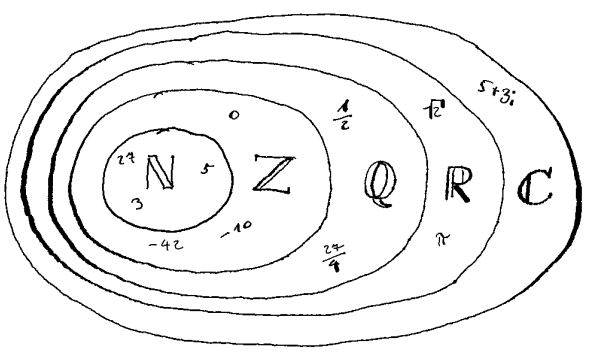
\includegraphics[width=0.6\textwidth]{img/zahlen.png}
    \caption{Zahlen als Euler Diagramm. }
    \label{fig:zahlen}
\end{figure}



Die Arten Mengen in Beziehung zu setzen kann verwendet werden um die unterschiedlichen Zahlen Korpora in Beziehung zu setzen:

$$
\mathbb{N} \subset \mathbb{Z} \subset \mathbb{Q} \subset \mathbb{R} \subset \mathbb{C}
 $$

Siehe auch Abbildung \ref{fig:zahlen}. Im Folgenden ein paar Worte zu den unterschiedlichen Mengen.



\subsection{Natürliche Zahlen $\mathbb{N}$}
Ganzzahlen beginnend bei $1$. Also $\{1,2,3,4,...\}$. Manchmal wir hier die Zahl $0$ inkludiert wenn es in dem Zusammenhang praktisch ist. Dies wird typischerweise so markiert: $\mathbb{N}_0$.  
\subsection{Ganze Zahlen $\mathbb{Z}$}
Alle Ganzzahlen inkl. $0$ und negativen Zahlen.
\subsection{Rationale Zahlen $\mathbb{Q}$}
Zahlen die als Brüche von Ganzzahlen ausgedrückt werden können. zB. $5$ $\frac{1}{2}$ oder $\frac{1}{3}$.

\subsection{Reelle Zahlen $\mathbb{R}$}
\index{Reelle Zahlen}
Reelle Zahlen füllen die 'Lücken' zwischen den Rationalen Zahlen. Enthalten sind auch irrationale Zahlen wie $\pi$ oder $\sqrt{2}$.



\begin{figure}[h!]
    \centering
    

\begin{tikzpicture}
    % Draw the number line from -4 to 4
    \draw[->] (-4.5,0) -- (4.5,0) node[below] {$\mathbb{R}$}; % The real number line
    
    % Draw ticks at whole number intervals
    \foreach \x in {-4,-3,-2,-1,0,1,2,3,4}
      \draw (\x,0) -- (\x,0.2);
      
    % Label the whole numbers below the number line
    \foreach \x in {-4,-3,-2,-1,0,1,2,3,4}
      \node at (\x,-0.3) {\x};

    % Mark and label pi above
    \draw (3.14,0) -- (3.14,0.2) node[above] {$\pi$};
    
    % Mark and label -sqrt(2) above
    \draw (-1.414,0) -- (-1.414,0.2) node[above] {$-\sqrt{2}$};
    
    % Add dashed lines for pi and -sqrt(2)
    \draw[dashed] (3.14,0) -- (3.14,-0.5);
    \draw[dashed] (-1.414,0) -- (-1.414,-0.5);

\end{tikzpicture}
    \caption{Zahlengerade.}
    \label{fig:zahlengerade}
\end{figure}


\subsection{Komplexe Zahlen $\mathbb{C}$}
\index{Komplexe Zahlen}
Besonders wichtig für die Tontechnik, hierzu mehr in Kapitel \ref{chap:complex}. Erweiterung der Zahlengeraden (siehe Abb. \ref{fig:zahlengerade}) auf die 'Komplexe Ebene'. Sie dienen uns zur Darstellung von Schwingungen, kommen vor in der Fouriertransformation (bei jeder Berechnung eines klassischen Audio Spektrums!) etc. \
Es gibt noch weitere Zahlen Mengen, zum Beispiel die \emph{Quaternionen}, eine Erweiterung der Komplexen Zahlen. Diese finden zum Beispiel Anwendung in der Grafik Verarbeitung (in mehr oder weniger jeder 3D Animation zB.). 


\todo[inline]{Intervalle?}

\section{Rechenoperationen}

Einfache Rechenoperationen wie $+, -, \cdot, / $, haben in der Tontechnik/Signalverarbeitung direkt fassbare Bedeutungen.


\begin{figure}[h!]
    \centering
        %% Creator: Matplotlib, PGF backend
%%
%% To include the figure in your LaTeX document, write
%%   \input{<filename>.pgf}
%%
%% Make sure the required packages are loaded in your preamble
%%   \usepackage{pgf}
%%
%% Also ensure that all the required font packages are loaded; for instance,
%% the lmodern package is sometimes necessary when using math font.
%%   \usepackage{lmodern}
%%
%% Figures using additional raster images can only be included by \input if
%% they are in the same directory as the main LaTeX file. For loading figures
%% from other directories you can use the `import` package
%%   \usepackage{import}
%%
%% and then include the figures with
%%   \import{<path to file>}{<filename>.pgf}
%%
%% Matplotlib used the following preamble
%%   \def\mathdefault#1{#1}
%%   \everymath=\expandafter{\the\everymath\displaystyle}
%%   
%%   \usepackage{fontspec}
%%   \setmainfont{VeraSe.ttf}[Path=\detokenize{/usr/share/fonts/TTF/}]
%%   \setsansfont{DejaVuSans.ttf}[Path=\detokenize{/home/pl/miniconda3/lib/python3.12/site-packages/matplotlib/mpl-data/fonts/ttf/}]
%%   \setmonofont{DejaVuSansMono.ttf}[Path=\detokenize{/home/pl/miniconda3/lib/python3.12/site-packages/matplotlib/mpl-data/fonts/ttf/}]
%%   \makeatletter\@ifpackageloaded{underscore}{}{\usepackage[strings]{underscore}}\makeatother
%%
\begingroup%
\makeatletter%
\begin{pgfpicture}%
\pgfpathrectangle{\pgfpointorigin}{\pgfqpoint{6.093662in}{2.027596in}}%
\pgfusepath{use as bounding box, clip}%
\begin{pgfscope}%
\pgfsetbuttcap%
\pgfsetmiterjoin%
\definecolor{currentfill}{rgb}{1.000000,1.000000,1.000000}%
\pgfsetfillcolor{currentfill}%
\pgfsetlinewidth{0.000000pt}%
\definecolor{currentstroke}{rgb}{1.000000,1.000000,1.000000}%
\pgfsetstrokecolor{currentstroke}%
\pgfsetdash{}{0pt}%
\pgfpathmoveto{\pgfqpoint{0.000000in}{0.000000in}}%
\pgfpathlineto{\pgfqpoint{6.093662in}{0.000000in}}%
\pgfpathlineto{\pgfqpoint{6.093662in}{2.027596in}}%
\pgfpathlineto{\pgfqpoint{0.000000in}{2.027596in}}%
\pgfpathlineto{\pgfqpoint{0.000000in}{0.000000in}}%
\pgfpathclose%
\pgfusepath{fill}%
\end{pgfscope}%
\begin{pgfscope}%
\pgfsetbuttcap%
\pgfsetmiterjoin%
\definecolor{currentfill}{rgb}{1.000000,1.000000,1.000000}%
\pgfsetfillcolor{currentfill}%
\pgfsetlinewidth{0.000000pt}%
\definecolor{currentstroke}{rgb}{0.000000,0.000000,0.000000}%
\pgfsetstrokecolor{currentstroke}%
\pgfsetstrokeopacity{0.000000}%
\pgfsetdash{}{0pt}%
\pgfpathmoveto{\pgfqpoint{0.526127in}{0.331635in}}%
\pgfpathlineto{\pgfqpoint{2.992036in}{0.331635in}}%
\pgfpathlineto{\pgfqpoint{2.992036in}{1.717635in}}%
\pgfpathlineto{\pgfqpoint{0.526127in}{1.717635in}}%
\pgfpathlineto{\pgfqpoint{0.526127in}{0.331635in}}%
\pgfpathclose%
\pgfusepath{fill}%
\end{pgfscope}%
\begin{pgfscope}%
\pgfsetbuttcap%
\pgfsetroundjoin%
\definecolor{currentfill}{rgb}{0.000000,0.000000,0.000000}%
\pgfsetfillcolor{currentfill}%
\pgfsetlinewidth{0.803000pt}%
\definecolor{currentstroke}{rgb}{0.000000,0.000000,0.000000}%
\pgfsetstrokecolor{currentstroke}%
\pgfsetdash{}{0pt}%
\pgfsys@defobject{currentmarker}{\pgfqpoint{0.000000in}{-0.048611in}}{\pgfqpoint{0.000000in}{0.000000in}}{%
\pgfpathmoveto{\pgfqpoint{0.000000in}{0.000000in}}%
\pgfpathlineto{\pgfqpoint{0.000000in}{-0.048611in}}%
\pgfusepath{stroke,fill}%
}%
\begin{pgfscope}%
\pgfsys@transformshift{0.638213in}{0.331635in}%
\pgfsys@useobject{currentmarker}{}%
\end{pgfscope}%
\end{pgfscope}%
\begin{pgfscope}%
\definecolor{textcolor}{rgb}{0.000000,0.000000,0.000000}%
\pgfsetstrokecolor{textcolor}%
\pgfsetfillcolor{textcolor}%
\pgftext[x=0.638213in,y=0.234413in,,top]{\color{textcolor}{\rmfamily\fontsize{10.000000}{12.000000}\selectfont\catcode`\^=\active\def^{\ifmmode\sp\else\^{}\fi}\catcode`\%=\active\def%{\%}0.00}}%
\end{pgfscope}%
\begin{pgfscope}%
\pgfsetbuttcap%
\pgfsetroundjoin%
\definecolor{currentfill}{rgb}{0.000000,0.000000,0.000000}%
\pgfsetfillcolor{currentfill}%
\pgfsetlinewidth{0.803000pt}%
\definecolor{currentstroke}{rgb}{0.000000,0.000000,0.000000}%
\pgfsetstrokecolor{currentstroke}%
\pgfsetdash{}{0pt}%
\pgfsys@defobject{currentmarker}{\pgfqpoint{0.000000in}{-0.048611in}}{\pgfqpoint{0.000000in}{0.000000in}}{%
\pgfpathmoveto{\pgfqpoint{0.000000in}{0.000000in}}%
\pgfpathlineto{\pgfqpoint{0.000000in}{-0.048611in}}%
\pgfusepath{stroke,fill}%
}%
\begin{pgfscope}%
\pgfsys@transformshift{1.198647in}{0.331635in}%
\pgfsys@useobject{currentmarker}{}%
\end{pgfscope}%
\end{pgfscope}%
\begin{pgfscope}%
\definecolor{textcolor}{rgb}{0.000000,0.000000,0.000000}%
\pgfsetstrokecolor{textcolor}%
\pgfsetfillcolor{textcolor}%
\pgftext[x=1.198647in,y=0.234413in,,top]{\color{textcolor}{\rmfamily\fontsize{10.000000}{12.000000}\selectfont\catcode`\^=\active\def^{\ifmmode\sp\else\^{}\fi}\catcode`\%=\active\def%{\%}0.25}}%
\end{pgfscope}%
\begin{pgfscope}%
\pgfsetbuttcap%
\pgfsetroundjoin%
\definecolor{currentfill}{rgb}{0.000000,0.000000,0.000000}%
\pgfsetfillcolor{currentfill}%
\pgfsetlinewidth{0.803000pt}%
\definecolor{currentstroke}{rgb}{0.000000,0.000000,0.000000}%
\pgfsetstrokecolor{currentstroke}%
\pgfsetdash{}{0pt}%
\pgfsys@defobject{currentmarker}{\pgfqpoint{0.000000in}{-0.048611in}}{\pgfqpoint{0.000000in}{0.000000in}}{%
\pgfpathmoveto{\pgfqpoint{0.000000in}{0.000000in}}%
\pgfpathlineto{\pgfqpoint{0.000000in}{-0.048611in}}%
\pgfusepath{stroke,fill}%
}%
\begin{pgfscope}%
\pgfsys@transformshift{1.759081in}{0.331635in}%
\pgfsys@useobject{currentmarker}{}%
\end{pgfscope}%
\end{pgfscope}%
\begin{pgfscope}%
\definecolor{textcolor}{rgb}{0.000000,0.000000,0.000000}%
\pgfsetstrokecolor{textcolor}%
\pgfsetfillcolor{textcolor}%
\pgftext[x=1.759081in,y=0.234413in,,top]{\color{textcolor}{\rmfamily\fontsize{10.000000}{12.000000}\selectfont\catcode`\^=\active\def^{\ifmmode\sp\else\^{}\fi}\catcode`\%=\active\def%{\%}0.50}}%
\end{pgfscope}%
\begin{pgfscope}%
\pgfsetbuttcap%
\pgfsetroundjoin%
\definecolor{currentfill}{rgb}{0.000000,0.000000,0.000000}%
\pgfsetfillcolor{currentfill}%
\pgfsetlinewidth{0.803000pt}%
\definecolor{currentstroke}{rgb}{0.000000,0.000000,0.000000}%
\pgfsetstrokecolor{currentstroke}%
\pgfsetdash{}{0pt}%
\pgfsys@defobject{currentmarker}{\pgfqpoint{0.000000in}{-0.048611in}}{\pgfqpoint{0.000000in}{0.000000in}}{%
\pgfpathmoveto{\pgfqpoint{0.000000in}{0.000000in}}%
\pgfpathlineto{\pgfqpoint{0.000000in}{-0.048611in}}%
\pgfusepath{stroke,fill}%
}%
\begin{pgfscope}%
\pgfsys@transformshift{2.319515in}{0.331635in}%
\pgfsys@useobject{currentmarker}{}%
\end{pgfscope}%
\end{pgfscope}%
\begin{pgfscope}%
\definecolor{textcolor}{rgb}{0.000000,0.000000,0.000000}%
\pgfsetstrokecolor{textcolor}%
\pgfsetfillcolor{textcolor}%
\pgftext[x=2.319515in,y=0.234413in,,top]{\color{textcolor}{\rmfamily\fontsize{10.000000}{12.000000}\selectfont\catcode`\^=\active\def^{\ifmmode\sp\else\^{}\fi}\catcode`\%=\active\def%{\%}0.75}}%
\end{pgfscope}%
\begin{pgfscope}%
\pgfsetbuttcap%
\pgfsetroundjoin%
\definecolor{currentfill}{rgb}{0.000000,0.000000,0.000000}%
\pgfsetfillcolor{currentfill}%
\pgfsetlinewidth{0.803000pt}%
\definecolor{currentstroke}{rgb}{0.000000,0.000000,0.000000}%
\pgfsetstrokecolor{currentstroke}%
\pgfsetdash{}{0pt}%
\pgfsys@defobject{currentmarker}{\pgfqpoint{0.000000in}{-0.048611in}}{\pgfqpoint{0.000000in}{0.000000in}}{%
\pgfpathmoveto{\pgfqpoint{0.000000in}{0.000000in}}%
\pgfpathlineto{\pgfqpoint{0.000000in}{-0.048611in}}%
\pgfusepath{stroke,fill}%
}%
\begin{pgfscope}%
\pgfsys@transformshift{2.879949in}{0.331635in}%
\pgfsys@useobject{currentmarker}{}%
\end{pgfscope}%
\end{pgfscope}%
\begin{pgfscope}%
\definecolor{textcolor}{rgb}{0.000000,0.000000,0.000000}%
\pgfsetstrokecolor{textcolor}%
\pgfsetfillcolor{textcolor}%
\pgftext[x=2.879949in,y=0.234413in,,top]{\color{textcolor}{\rmfamily\fontsize{10.000000}{12.000000}\selectfont\catcode`\^=\active\def^{\ifmmode\sp\else\^{}\fi}\catcode`\%=\active\def%{\%}1.00}}%
\end{pgfscope}%
\begin{pgfscope}%
\pgfsetbuttcap%
\pgfsetroundjoin%
\definecolor{currentfill}{rgb}{0.000000,0.000000,0.000000}%
\pgfsetfillcolor{currentfill}%
\pgfsetlinewidth{0.803000pt}%
\definecolor{currentstroke}{rgb}{0.000000,0.000000,0.000000}%
\pgfsetstrokecolor{currentstroke}%
\pgfsetdash{}{0pt}%
\pgfsys@defobject{currentmarker}{\pgfqpoint{-0.048611in}{0.000000in}}{\pgfqpoint{-0.000000in}{0.000000in}}{%
\pgfpathmoveto{\pgfqpoint{-0.000000in}{0.000000in}}%
\pgfpathlineto{\pgfqpoint{-0.048611in}{0.000000in}}%
\pgfusepath{stroke,fill}%
}%
\begin{pgfscope}%
\pgfsys@transformshift{0.526127in}{0.331635in}%
\pgfsys@useobject{currentmarker}{}%
\end{pgfscope}%
\end{pgfscope}%
\begin{pgfscope}%
\definecolor{textcolor}{rgb}{0.000000,0.000000,0.000000}%
\pgfsetstrokecolor{textcolor}%
\pgfsetfillcolor{textcolor}%
\pgftext[x=0.100000in, y=0.278873in, left, base]{\color{textcolor}{\rmfamily\fontsize{10.000000}{12.000000}\selectfont\catcode`\^=\active\def^{\ifmmode\sp\else\^{}\fi}\catcode`\%=\active\def%{\%}\ensuremath{-}1.0}}%
\end{pgfscope}%
\begin{pgfscope}%
\pgfsetbuttcap%
\pgfsetroundjoin%
\definecolor{currentfill}{rgb}{0.000000,0.000000,0.000000}%
\pgfsetfillcolor{currentfill}%
\pgfsetlinewidth{0.803000pt}%
\definecolor{currentstroke}{rgb}{0.000000,0.000000,0.000000}%
\pgfsetstrokecolor{currentstroke}%
\pgfsetdash{}{0pt}%
\pgfsys@defobject{currentmarker}{\pgfqpoint{-0.048611in}{0.000000in}}{\pgfqpoint{-0.000000in}{0.000000in}}{%
\pgfpathmoveto{\pgfqpoint{-0.000000in}{0.000000in}}%
\pgfpathlineto{\pgfqpoint{-0.048611in}{0.000000in}}%
\pgfusepath{stroke,fill}%
}%
\begin{pgfscope}%
\pgfsys@transformshift{0.526127in}{0.678135in}%
\pgfsys@useobject{currentmarker}{}%
\end{pgfscope}%
\end{pgfscope}%
\begin{pgfscope}%
\definecolor{textcolor}{rgb}{0.000000,0.000000,0.000000}%
\pgfsetstrokecolor{textcolor}%
\pgfsetfillcolor{textcolor}%
\pgftext[x=0.100000in, y=0.625373in, left, base]{\color{textcolor}{\rmfamily\fontsize{10.000000}{12.000000}\selectfont\catcode`\^=\active\def^{\ifmmode\sp\else\^{}\fi}\catcode`\%=\active\def%{\%}\ensuremath{-}0.5}}%
\end{pgfscope}%
\begin{pgfscope}%
\pgfsetbuttcap%
\pgfsetroundjoin%
\definecolor{currentfill}{rgb}{0.000000,0.000000,0.000000}%
\pgfsetfillcolor{currentfill}%
\pgfsetlinewidth{0.803000pt}%
\definecolor{currentstroke}{rgb}{0.000000,0.000000,0.000000}%
\pgfsetstrokecolor{currentstroke}%
\pgfsetdash{}{0pt}%
\pgfsys@defobject{currentmarker}{\pgfqpoint{-0.048611in}{0.000000in}}{\pgfqpoint{-0.000000in}{0.000000in}}{%
\pgfpathmoveto{\pgfqpoint{-0.000000in}{0.000000in}}%
\pgfpathlineto{\pgfqpoint{-0.048611in}{0.000000in}}%
\pgfusepath{stroke,fill}%
}%
\begin{pgfscope}%
\pgfsys@transformshift{0.526127in}{1.024635in}%
\pgfsys@useobject{currentmarker}{}%
\end{pgfscope}%
\end{pgfscope}%
\begin{pgfscope}%
\definecolor{textcolor}{rgb}{0.000000,0.000000,0.000000}%
\pgfsetstrokecolor{textcolor}%
\pgfsetfillcolor{textcolor}%
\pgftext[x=0.208025in, y=0.971873in, left, base]{\color{textcolor}{\rmfamily\fontsize{10.000000}{12.000000}\selectfont\catcode`\^=\active\def^{\ifmmode\sp\else\^{}\fi}\catcode`\%=\active\def%{\%}0.0}}%
\end{pgfscope}%
\begin{pgfscope}%
\pgfsetbuttcap%
\pgfsetroundjoin%
\definecolor{currentfill}{rgb}{0.000000,0.000000,0.000000}%
\pgfsetfillcolor{currentfill}%
\pgfsetlinewidth{0.803000pt}%
\definecolor{currentstroke}{rgb}{0.000000,0.000000,0.000000}%
\pgfsetstrokecolor{currentstroke}%
\pgfsetdash{}{0pt}%
\pgfsys@defobject{currentmarker}{\pgfqpoint{-0.048611in}{0.000000in}}{\pgfqpoint{-0.000000in}{0.000000in}}{%
\pgfpathmoveto{\pgfqpoint{-0.000000in}{0.000000in}}%
\pgfpathlineto{\pgfqpoint{-0.048611in}{0.000000in}}%
\pgfusepath{stroke,fill}%
}%
\begin{pgfscope}%
\pgfsys@transformshift{0.526127in}{1.371135in}%
\pgfsys@useobject{currentmarker}{}%
\end{pgfscope}%
\end{pgfscope}%
\begin{pgfscope}%
\definecolor{textcolor}{rgb}{0.000000,0.000000,0.000000}%
\pgfsetstrokecolor{textcolor}%
\pgfsetfillcolor{textcolor}%
\pgftext[x=0.208025in, y=1.318373in, left, base]{\color{textcolor}{\rmfamily\fontsize{10.000000}{12.000000}\selectfont\catcode`\^=\active\def^{\ifmmode\sp\else\^{}\fi}\catcode`\%=\active\def%{\%}0.5}}%
\end{pgfscope}%
\begin{pgfscope}%
\pgfsetbuttcap%
\pgfsetroundjoin%
\definecolor{currentfill}{rgb}{0.000000,0.000000,0.000000}%
\pgfsetfillcolor{currentfill}%
\pgfsetlinewidth{0.803000pt}%
\definecolor{currentstroke}{rgb}{0.000000,0.000000,0.000000}%
\pgfsetstrokecolor{currentstroke}%
\pgfsetdash{}{0pt}%
\pgfsys@defobject{currentmarker}{\pgfqpoint{-0.048611in}{0.000000in}}{\pgfqpoint{-0.000000in}{0.000000in}}{%
\pgfpathmoveto{\pgfqpoint{-0.000000in}{0.000000in}}%
\pgfpathlineto{\pgfqpoint{-0.048611in}{0.000000in}}%
\pgfusepath{stroke,fill}%
}%
\begin{pgfscope}%
\pgfsys@transformshift{0.526127in}{1.717635in}%
\pgfsys@useobject{currentmarker}{}%
\end{pgfscope}%
\end{pgfscope}%
\begin{pgfscope}%
\definecolor{textcolor}{rgb}{0.000000,0.000000,0.000000}%
\pgfsetstrokecolor{textcolor}%
\pgfsetfillcolor{textcolor}%
\pgftext[x=0.208025in, y=1.664873in, left, base]{\color{textcolor}{\rmfamily\fontsize{10.000000}{12.000000}\selectfont\catcode`\^=\active\def^{\ifmmode\sp\else\^{}\fi}\catcode`\%=\active\def%{\%}1.0}}%
\end{pgfscope}%
\begin{pgfscope}%
\pgfpathrectangle{\pgfqpoint{0.526127in}{0.331635in}}{\pgfqpoint{2.465909in}{1.386000in}}%
\pgfusepath{clip}%
\pgfsetrectcap%
\pgfsetroundjoin%
\pgfsetlinewidth{1.505625pt}%
\definecolor{currentstroke}{rgb}{0.000000,0.000000,0.000000}%
\pgfsetstrokecolor{currentstroke}%
\pgfsetdash{}{0pt}%
\pgfpathmoveto{\pgfqpoint{0.638213in}{1.371135in}}%
\pgfpathlineto{\pgfqpoint{0.658551in}{1.445932in}}%
\pgfpathlineto{\pgfqpoint{0.669229in}{1.477008in}}%
\pgfpathlineto{\pgfqpoint{0.677364in}{1.494487in}}%
\pgfpathlineto{\pgfqpoint{0.683974in}{1.504018in}}%
\pgfpathlineto{\pgfqpoint{0.689566in}{1.508539in}}%
\pgfpathlineto{\pgfqpoint{0.694142in}{1.509734in}}%
\pgfpathlineto{\pgfqpoint{0.698718in}{1.508653in}}%
\pgfpathlineto{\pgfqpoint{0.703803in}{1.504803in}}%
\pgfpathlineto{\pgfqpoint{0.709396in}{1.497444in}}%
\pgfpathlineto{\pgfqpoint{0.716006in}{1.484772in}}%
\pgfpathlineto{\pgfqpoint{0.724141in}{1.463894in}}%
\pgfpathlineto{\pgfqpoint{0.734310in}{1.431195in}}%
\pgfpathlineto{\pgfqpoint{0.750580in}{1.370049in}}%
\pgfpathlineto{\pgfqpoint{0.770918in}{1.295426in}}%
\pgfpathlineto{\pgfqpoint{0.781595in}{1.264564in}}%
\pgfpathlineto{\pgfqpoint{0.789730in}{1.247291in}}%
\pgfpathlineto{\pgfqpoint{0.796340in}{1.237947in}}%
\pgfpathlineto{\pgfqpoint{0.801933in}{1.233593in}}%
\pgfpathlineto{\pgfqpoint{0.806509in}{1.232536in}}%
\pgfpathlineto{\pgfqpoint{0.811085in}{1.233757in}}%
\pgfpathlineto{\pgfqpoint{0.816169in}{1.237758in}}%
\pgfpathlineto{\pgfqpoint{0.821762in}{1.245277in}}%
\pgfpathlineto{\pgfqpoint{0.828372in}{1.258124in}}%
\pgfpathlineto{\pgfqpoint{0.836507in}{1.279186in}}%
\pgfpathlineto{\pgfqpoint{0.847184in}{1.313849in}}%
\pgfpathlineto{\pgfqpoint{0.864472in}{1.379229in}}%
\pgfpathlineto{\pgfqpoint{0.883284in}{1.447752in}}%
\pgfpathlineto{\pgfqpoint{0.893453in}{1.477136in}}%
\pgfpathlineto{\pgfqpoint{0.901588in}{1.494577in}}%
\pgfpathlineto{\pgfqpoint{0.908198in}{1.504074in}}%
\pgfpathlineto{\pgfqpoint{0.913791in}{1.508565in}}%
\pgfpathlineto{\pgfqpoint{0.918367in}{1.509735in}}%
\pgfpathlineto{\pgfqpoint{0.922943in}{1.508628in}}%
\pgfpathlineto{\pgfqpoint{0.928027in}{1.504751in}}%
\pgfpathlineto{\pgfqpoint{0.933620in}{1.497362in}}%
\pgfpathlineto{\pgfqpoint{0.940230in}{1.484658in}}%
\pgfpathlineto{\pgfqpoint{0.948365in}{1.463747in}}%
\pgfpathlineto{\pgfqpoint{0.958534in}{1.431017in}}%
\pgfpathlineto{\pgfqpoint{0.974804in}{1.369851in}}%
\pgfpathlineto{\pgfqpoint{0.995142in}{1.295261in}}%
\pgfpathlineto{\pgfqpoint{1.005819in}{1.264438in}}%
\pgfpathlineto{\pgfqpoint{1.013955in}{1.247203in}}%
\pgfpathlineto{\pgfqpoint{1.020564in}{1.237893in}}%
\pgfpathlineto{\pgfqpoint{1.026157in}{1.233569in}}%
\pgfpathlineto{\pgfqpoint{1.030733in}{1.232538in}}%
\pgfpathlineto{\pgfqpoint{1.035309in}{1.233783in}}%
\pgfpathlineto{\pgfqpoint{1.040394in}{1.237812in}}%
\pgfpathlineto{\pgfqpoint{1.045987in}{1.245360in}}%
\pgfpathlineto{\pgfqpoint{1.052596in}{1.258238in}}%
\pgfpathlineto{\pgfqpoint{1.060732in}{1.279334in}}%
\pgfpathlineto{\pgfqpoint{1.071409in}{1.314028in}}%
\pgfpathlineto{\pgfqpoint{1.088696in}{1.379426in}}%
\pgfpathlineto{\pgfqpoint{1.107508in}{1.447916in}}%
\pgfpathlineto{\pgfqpoint{1.117677in}{1.477263in}}%
\pgfpathlineto{\pgfqpoint{1.125813in}{1.494667in}}%
\pgfpathlineto{\pgfqpoint{1.132422in}{1.504130in}}%
\pgfpathlineto{\pgfqpoint{1.138015in}{1.508590in}}%
\pgfpathlineto{\pgfqpoint{1.142591in}{1.509735in}}%
\pgfpathlineto{\pgfqpoint{1.147167in}{1.508603in}}%
\pgfpathlineto{\pgfqpoint{1.152252in}{1.504699in}}%
\pgfpathlineto{\pgfqpoint{1.157845in}{1.497281in}}%
\pgfpathlineto{\pgfqpoint{1.164454in}{1.484545in}}%
\pgfpathlineto{\pgfqpoint{1.172590in}{1.463600in}}%
\pgfpathlineto{\pgfqpoint{1.182758in}{1.430839in}}%
\pgfpathlineto{\pgfqpoint{1.199029in}{1.369654in}}%
\pgfpathlineto{\pgfqpoint{1.219366in}{1.295095in}}%
\pgfpathlineto{\pgfqpoint{1.230044in}{1.264312in}}%
\pgfpathlineto{\pgfqpoint{1.238179in}{1.247115in}}%
\pgfpathlineto{\pgfqpoint{1.244789in}{1.237839in}}%
\pgfpathlineto{\pgfqpoint{1.250382in}{1.233545in}}%
\pgfpathlineto{\pgfqpoint{1.254958in}{1.232539in}}%
\pgfpathlineto{\pgfqpoint{1.259534in}{1.233810in}}%
\pgfpathlineto{\pgfqpoint{1.264618in}{1.237866in}}%
\pgfpathlineto{\pgfqpoint{1.270211in}{1.245443in}}%
\pgfpathlineto{\pgfqpoint{1.276821in}{1.258353in}}%
\pgfpathlineto{\pgfqpoint{1.284956in}{1.279482in}}%
\pgfpathlineto{\pgfqpoint{1.295633in}{1.314208in}}%
\pgfpathlineto{\pgfqpoint{1.312920in}{1.379623in}}%
\pgfpathlineto{\pgfqpoint{1.331224in}{1.446430in}}%
\pgfpathlineto{\pgfqpoint{1.341902in}{1.477390in}}%
\pgfpathlineto{\pgfqpoint{1.350037in}{1.494756in}}%
\pgfpathlineto{\pgfqpoint{1.356647in}{1.504185in}}%
\pgfpathlineto{\pgfqpoint{1.362240in}{1.508615in}}%
\pgfpathlineto{\pgfqpoint{1.366816in}{1.509735in}}%
\pgfpathlineto{\pgfqpoint{1.371392in}{1.508578in}}%
\pgfpathlineto{\pgfqpoint{1.376476in}{1.504646in}}%
\pgfpathlineto{\pgfqpoint{1.382069in}{1.497199in}}%
\pgfpathlineto{\pgfqpoint{1.388679in}{1.484431in}}%
\pgfpathlineto{\pgfqpoint{1.396814in}{1.463452in}}%
\pgfpathlineto{\pgfqpoint{1.406983in}{1.430660in}}%
\pgfpathlineto{\pgfqpoint{1.423253in}{1.369456in}}%
\pgfpathlineto{\pgfqpoint{1.443082in}{1.296588in}}%
\pgfpathlineto{\pgfqpoint{1.453760in}{1.265453in}}%
\pgfpathlineto{\pgfqpoint{1.461895in}{1.247918in}}%
\pgfpathlineto{\pgfqpoint{1.468505in}{1.238337in}}%
\pgfpathlineto{\pgfqpoint{1.474098in}{1.233770in}}%
\pgfpathlineto{\pgfqpoint{1.478674in}{1.232537in}}%
\pgfpathlineto{\pgfqpoint{1.483250in}{1.233581in}}%
\pgfpathlineto{\pgfqpoint{1.487826in}{1.236884in}}%
\pgfpathlineto{\pgfqpoint{1.493419in}{1.243908in}}%
\pgfpathlineto{\pgfqpoint{1.500028in}{1.256213in}}%
\pgfpathlineto{\pgfqpoint{1.508163in}{1.276701in}}%
\pgfpathlineto{\pgfqpoint{1.518332in}{1.309036in}}%
\pgfpathlineto{\pgfqpoint{1.534094in}{1.367975in}}%
\pgfpathlineto{\pgfqpoint{1.555449in}{1.446596in}}%
\pgfpathlineto{\pgfqpoint{1.566126in}{1.477517in}}%
\pgfpathlineto{\pgfqpoint{1.574261in}{1.494845in}}%
\pgfpathlineto{\pgfqpoint{1.580871in}{1.504240in}}%
\pgfpathlineto{\pgfqpoint{1.586464in}{1.508640in}}%
\pgfpathlineto{\pgfqpoint{1.591040in}{1.509735in}}%
\pgfpathlineto{\pgfqpoint{1.595616in}{1.508552in}}%
\pgfpathlineto{\pgfqpoint{1.600700in}{1.504592in}}%
\pgfpathlineto{\pgfqpoint{1.606293in}{1.497117in}}%
\pgfpathlineto{\pgfqpoint{1.612903in}{1.484317in}}%
\pgfpathlineto{\pgfqpoint{1.621038in}{1.463305in}}%
\pgfpathlineto{\pgfqpoint{1.631207in}{1.430482in}}%
\pgfpathlineto{\pgfqpoint{1.647477in}{1.369259in}}%
\pgfpathlineto{\pgfqpoint{1.667307in}{1.296421in}}%
\pgfpathlineto{\pgfqpoint{1.677984in}{1.265325in}}%
\pgfpathlineto{\pgfqpoint{1.686119in}{1.247828in}}%
\pgfpathlineto{\pgfqpoint{1.692729in}{1.238280in}}%
\pgfpathlineto{\pgfqpoint{1.698322in}{1.233744in}}%
\pgfpathlineto{\pgfqpoint{1.702898in}{1.232536in}}%
\pgfpathlineto{\pgfqpoint{1.707474in}{1.233605in}}%
\pgfpathlineto{\pgfqpoint{1.712558in}{1.237440in}}%
\pgfpathlineto{\pgfqpoint{1.718151in}{1.244785in}}%
\pgfpathlineto{\pgfqpoint{1.724761in}{1.257442in}}%
\pgfpathlineto{\pgfqpoint{1.732896in}{1.278303in}}%
\pgfpathlineto{\pgfqpoint{1.743065in}{1.310986in}}%
\pgfpathlineto{\pgfqpoint{1.759335in}{1.372123in}}%
\pgfpathlineto{\pgfqpoint{1.779673in}{1.446761in}}%
\pgfpathlineto{\pgfqpoint{1.790351in}{1.477643in}}%
\pgfpathlineto{\pgfqpoint{1.798486in}{1.494934in}}%
\pgfpathlineto{\pgfqpoint{1.805096in}{1.504295in}}%
\pgfpathlineto{\pgfqpoint{1.810688in}{1.508665in}}%
\pgfpathlineto{\pgfqpoint{1.815264in}{1.509734in}}%
\pgfpathlineto{\pgfqpoint{1.819840in}{1.508526in}}%
\pgfpathlineto{\pgfqpoint{1.824925in}{1.504539in}}%
\pgfpathlineto{\pgfqpoint{1.830518in}{1.497034in}}%
\pgfpathlineto{\pgfqpoint{1.837128in}{1.484203in}}%
\pgfpathlineto{\pgfqpoint{1.845263in}{1.463157in}}%
\pgfpathlineto{\pgfqpoint{1.855432in}{1.430303in}}%
\pgfpathlineto{\pgfqpoint{1.871702in}{1.369061in}}%
\pgfpathlineto{\pgfqpoint{1.891531in}{1.296255in}}%
\pgfpathlineto{\pgfqpoint{1.902209in}{1.265198in}}%
\pgfpathlineto{\pgfqpoint{1.910344in}{1.247738in}}%
\pgfpathlineto{\pgfqpoint{1.916953in}{1.238224in}}%
\pgfpathlineto{\pgfqpoint{1.922546in}{1.233718in}}%
\pgfpathlineto{\pgfqpoint{1.927122in}{1.232535in}}%
\pgfpathlineto{\pgfqpoint{1.931698in}{1.233630in}}%
\pgfpathlineto{\pgfqpoint{1.936783in}{1.237493in}}%
\pgfpathlineto{\pgfqpoint{1.942376in}{1.244867in}}%
\pgfpathlineto{\pgfqpoint{1.948986in}{1.257555in}}%
\pgfpathlineto{\pgfqpoint{1.957121in}{1.278450in}}%
\pgfpathlineto{\pgfqpoint{1.967290in}{1.311164in}}%
\pgfpathlineto{\pgfqpoint{1.983560in}{1.372320in}}%
\pgfpathlineto{\pgfqpoint{2.003898in}{1.446927in}}%
\pgfpathlineto{\pgfqpoint{2.014575in}{1.477769in}}%
\pgfpathlineto{\pgfqpoint{2.022710in}{1.495023in}}%
\pgfpathlineto{\pgfqpoint{2.029320in}{1.504350in}}%
\pgfpathlineto{\pgfqpoint{2.034913in}{1.508689in}}%
\pgfpathlineto{\pgfqpoint{2.039489in}{1.509733in}}%
\pgfpathlineto{\pgfqpoint{2.044065in}{1.508500in}}%
\pgfpathlineto{\pgfqpoint{2.049149in}{1.504485in}}%
\pgfpathlineto{\pgfqpoint{2.054742in}{1.496951in}}%
\pgfpathlineto{\pgfqpoint{2.061352in}{1.484089in}}%
\pgfpathlineto{\pgfqpoint{2.069487in}{1.463010in}}%
\pgfpathlineto{\pgfqpoint{2.080164in}{1.428332in}}%
\pgfpathlineto{\pgfqpoint{2.097452in}{1.362943in}}%
\pgfpathlineto{\pgfqpoint{2.116264in}{1.294436in}}%
\pgfpathlineto{\pgfqpoint{2.126433in}{1.265071in}}%
\pgfpathlineto{\pgfqpoint{2.134568in}{1.247648in}}%
\pgfpathlineto{\pgfqpoint{2.141178in}{1.238168in}}%
\pgfpathlineto{\pgfqpoint{2.146771in}{1.233692in}}%
\pgfpathlineto{\pgfqpoint{2.151347in}{1.232535in}}%
\pgfpathlineto{\pgfqpoint{2.155923in}{1.233655in}}%
\pgfpathlineto{\pgfqpoint{2.161007in}{1.237545in}}%
\pgfpathlineto{\pgfqpoint{2.166600in}{1.244948in}}%
\pgfpathlineto{\pgfqpoint{2.173210in}{1.257668in}}%
\pgfpathlineto{\pgfqpoint{2.181345in}{1.278597in}}%
\pgfpathlineto{\pgfqpoint{2.191514in}{1.311342in}}%
\pgfpathlineto{\pgfqpoint{2.207784in}{1.372518in}}%
\pgfpathlineto{\pgfqpoint{2.228122in}{1.447092in}}%
\pgfpathlineto{\pgfqpoint{2.238799in}{1.477895in}}%
\pgfpathlineto{\pgfqpoint{2.246935in}{1.495111in}}%
\pgfpathlineto{\pgfqpoint{2.253544in}{1.504404in}}%
\pgfpathlineto{\pgfqpoint{2.259137in}{1.508713in}}%
\pgfpathlineto{\pgfqpoint{2.263713in}{1.509732in}}%
\pgfpathlineto{\pgfqpoint{2.268289in}{1.508473in}}%
\pgfpathlineto{\pgfqpoint{2.273374in}{1.504431in}}%
\pgfpathlineto{\pgfqpoint{2.278967in}{1.496868in}}%
\pgfpathlineto{\pgfqpoint{2.285576in}{1.483974in}}%
\pgfpathlineto{\pgfqpoint{2.293711in}{1.462862in}}%
\pgfpathlineto{\pgfqpoint{2.304389in}{1.428152in}}%
\pgfpathlineto{\pgfqpoint{2.321676in}{1.362746in}}%
\pgfpathlineto{\pgfqpoint{2.340488in}{1.294272in}}%
\pgfpathlineto{\pgfqpoint{2.350657in}{1.264944in}}%
\pgfpathlineto{\pgfqpoint{2.358792in}{1.247559in}}%
\pgfpathlineto{\pgfqpoint{2.365402in}{1.238113in}}%
\pgfpathlineto{\pgfqpoint{2.370995in}{1.233667in}}%
\pgfpathlineto{\pgfqpoint{2.375571in}{1.232535in}}%
\pgfpathlineto{\pgfqpoint{2.380147in}{1.233680in}}%
\pgfpathlineto{\pgfqpoint{2.385232in}{1.237598in}}%
\pgfpathlineto{\pgfqpoint{2.390825in}{1.245030in}}%
\pgfpathlineto{\pgfqpoint{2.397434in}{1.257782in}}%
\pgfpathlineto{\pgfqpoint{2.405569in}{1.278744in}}%
\pgfpathlineto{\pgfqpoint{2.415738in}{1.311520in}}%
\pgfpathlineto{\pgfqpoint{2.432009in}{1.372715in}}%
\pgfpathlineto{\pgfqpoint{2.452346in}{1.447257in}}%
\pgfpathlineto{\pgfqpoint{2.463024in}{1.478021in}}%
\pgfpathlineto{\pgfqpoint{2.471159in}{1.495199in}}%
\pgfpathlineto{\pgfqpoint{2.477769in}{1.504458in}}%
\pgfpathlineto{\pgfqpoint{2.483362in}{1.508737in}}%
\pgfpathlineto{\pgfqpoint{2.487938in}{1.509730in}}%
\pgfpathlineto{\pgfqpoint{2.492514in}{1.508447in}}%
\pgfpathlineto{\pgfqpoint{2.497598in}{1.504377in}}%
\pgfpathlineto{\pgfqpoint{2.503191in}{1.496785in}}%
\pgfpathlineto{\pgfqpoint{2.509801in}{1.483860in}}%
\pgfpathlineto{\pgfqpoint{2.517936in}{1.462714in}}%
\pgfpathlineto{\pgfqpoint{2.528613in}{1.427971in}}%
\pgfpathlineto{\pgfqpoint{2.545900in}{1.362549in}}%
\pgfpathlineto{\pgfqpoint{2.564204in}{1.295757in}}%
\pgfpathlineto{\pgfqpoint{2.574882in}{1.264817in}}%
\pgfpathlineto{\pgfqpoint{2.583017in}{1.247469in}}%
\pgfpathlineto{\pgfqpoint{2.589627in}{1.238057in}}%
\pgfpathlineto{\pgfqpoint{2.595220in}{1.233642in}}%
\pgfpathlineto{\pgfqpoint{2.599796in}{1.232535in}}%
\pgfpathlineto{\pgfqpoint{2.604372in}{1.233705in}}%
\pgfpathlineto{\pgfqpoint{2.609456in}{1.237651in}}%
\pgfpathlineto{\pgfqpoint{2.615049in}{1.245112in}}%
\pgfpathlineto{\pgfqpoint{2.621659in}{1.257896in}}%
\pgfpathlineto{\pgfqpoint{2.629794in}{1.278891in}}%
\pgfpathlineto{\pgfqpoint{2.639963in}{1.311699in}}%
\pgfpathlineto{\pgfqpoint{2.656233in}{1.372913in}}%
\pgfpathlineto{\pgfqpoint{2.676062in}{1.445765in}}%
\pgfpathlineto{\pgfqpoint{2.686740in}{1.476881in}}%
\pgfpathlineto{\pgfqpoint{2.694875in}{1.494397in}}%
\pgfpathlineto{\pgfqpoint{2.701485in}{1.503962in}}%
\pgfpathlineto{\pgfqpoint{2.707078in}{1.508513in}}%
\pgfpathlineto{\pgfqpoint{2.711654in}{1.509734in}}%
\pgfpathlineto{\pgfqpoint{2.716230in}{1.508677in}}%
\pgfpathlineto{\pgfqpoint{2.720806in}{1.505361in}}%
\pgfpathlineto{\pgfqpoint{2.726398in}{1.498323in}}%
\pgfpathlineto{\pgfqpoint{2.733008in}{1.486002in}}%
\pgfpathlineto{\pgfqpoint{2.741143in}{1.465497in}}%
\pgfpathlineto{\pgfqpoint{2.751312in}{1.433146in}}%
\pgfpathlineto{\pgfqpoint{2.767074in}{1.374196in}}%
\pgfpathlineto{\pgfqpoint{2.788429in}{1.295591in}}%
\pgfpathlineto{\pgfqpoint{2.799106in}{1.264690in}}%
\pgfpathlineto{\pgfqpoint{2.807241in}{1.247380in}}%
\pgfpathlineto{\pgfqpoint{2.813851in}{1.238002in}}%
\pgfpathlineto{\pgfqpoint{2.819444in}{1.233617in}}%
\pgfpathlineto{\pgfqpoint{2.824020in}{1.232536in}}%
\pgfpathlineto{\pgfqpoint{2.828596in}{1.233731in}}%
\pgfpathlineto{\pgfqpoint{2.833680in}{1.237704in}}%
\pgfpathlineto{\pgfqpoint{2.839273in}{1.245195in}}%
\pgfpathlineto{\pgfqpoint{2.845883in}{1.258010in}}%
\pgfpathlineto{\pgfqpoint{2.854018in}{1.279039in}}%
\pgfpathlineto{\pgfqpoint{2.864187in}{1.311877in}}%
\pgfpathlineto{\pgfqpoint{2.879949in}{1.371135in}}%
\pgfpathlineto{\pgfqpoint{2.879949in}{1.371135in}}%
\pgfusepath{stroke}%
\end{pgfscope}%
\begin{pgfscope}%
\pgfpathrectangle{\pgfqpoint{0.526127in}{0.331635in}}{\pgfqpoint{2.465909in}{1.386000in}}%
\pgfusepath{clip}%
\pgfsetrectcap%
\pgfsetroundjoin%
\pgfsetlinewidth{0.501875pt}%
\definecolor{currentstroke}{rgb}{0.000000,0.000000,0.000000}%
\pgfsetstrokecolor{currentstroke}%
\pgfsetdash{}{0pt}%
\pgfpathmoveto{\pgfqpoint{0.526127in}{1.024635in}}%
\pgfpathlineto{\pgfqpoint{2.992036in}{1.024635in}}%
\pgfusepath{stroke}%
\end{pgfscope}%
\begin{pgfscope}%
\definecolor{textcolor}{rgb}{0.000000,0.000000,0.000000}%
\pgfsetstrokecolor{textcolor}%
\pgfsetfillcolor{textcolor}%
\pgftext[x=1.759081in,y=1.800968in,,base]{\color{textcolor}{\rmfamily\fontsize{12.000000}{14.400000}\selectfont\catcode`\^=\active\def^{\ifmmode\sp\else\^{}\fi}\catcode`\%=\active\def%{\%}Signal A}}%
\end{pgfscope}%
\begin{pgfscope}%
\pgfsetbuttcap%
\pgfsetmiterjoin%
\definecolor{currentfill}{rgb}{1.000000,1.000000,1.000000}%
\pgfsetfillcolor{currentfill}%
\pgfsetlinewidth{0.000000pt}%
\definecolor{currentstroke}{rgb}{0.000000,0.000000,0.000000}%
\pgfsetstrokecolor{currentstroke}%
\pgfsetstrokeopacity{0.000000}%
\pgfsetdash{}{0pt}%
\pgfpathmoveto{\pgfqpoint{3.485218in}{0.331635in}}%
\pgfpathlineto{\pgfqpoint{5.951127in}{0.331635in}}%
\pgfpathlineto{\pgfqpoint{5.951127in}{1.717635in}}%
\pgfpathlineto{\pgfqpoint{3.485218in}{1.717635in}}%
\pgfpathlineto{\pgfqpoint{3.485218in}{0.331635in}}%
\pgfpathclose%
\pgfusepath{fill}%
\end{pgfscope}%
\begin{pgfscope}%
\pgfsetbuttcap%
\pgfsetroundjoin%
\definecolor{currentfill}{rgb}{0.000000,0.000000,0.000000}%
\pgfsetfillcolor{currentfill}%
\pgfsetlinewidth{0.803000pt}%
\definecolor{currentstroke}{rgb}{0.000000,0.000000,0.000000}%
\pgfsetstrokecolor{currentstroke}%
\pgfsetdash{}{0pt}%
\pgfsys@defobject{currentmarker}{\pgfqpoint{0.000000in}{-0.048611in}}{\pgfqpoint{0.000000in}{0.000000in}}{%
\pgfpathmoveto{\pgfqpoint{0.000000in}{0.000000in}}%
\pgfpathlineto{\pgfqpoint{0.000000in}{-0.048611in}}%
\pgfusepath{stroke,fill}%
}%
\begin{pgfscope}%
\pgfsys@transformshift{3.597304in}{0.331635in}%
\pgfsys@useobject{currentmarker}{}%
\end{pgfscope}%
\end{pgfscope}%
\begin{pgfscope}%
\definecolor{textcolor}{rgb}{0.000000,0.000000,0.000000}%
\pgfsetstrokecolor{textcolor}%
\pgfsetfillcolor{textcolor}%
\pgftext[x=3.597304in,y=0.234413in,,top]{\color{textcolor}{\rmfamily\fontsize{10.000000}{12.000000}\selectfont\catcode`\^=\active\def^{\ifmmode\sp\else\^{}\fi}\catcode`\%=\active\def%{\%}0.00}}%
\end{pgfscope}%
\begin{pgfscope}%
\pgfsetbuttcap%
\pgfsetroundjoin%
\definecolor{currentfill}{rgb}{0.000000,0.000000,0.000000}%
\pgfsetfillcolor{currentfill}%
\pgfsetlinewidth{0.803000pt}%
\definecolor{currentstroke}{rgb}{0.000000,0.000000,0.000000}%
\pgfsetstrokecolor{currentstroke}%
\pgfsetdash{}{0pt}%
\pgfsys@defobject{currentmarker}{\pgfqpoint{0.000000in}{-0.048611in}}{\pgfqpoint{0.000000in}{0.000000in}}{%
\pgfpathmoveto{\pgfqpoint{0.000000in}{0.000000in}}%
\pgfpathlineto{\pgfqpoint{0.000000in}{-0.048611in}}%
\pgfusepath{stroke,fill}%
}%
\begin{pgfscope}%
\pgfsys@transformshift{4.157738in}{0.331635in}%
\pgfsys@useobject{currentmarker}{}%
\end{pgfscope}%
\end{pgfscope}%
\begin{pgfscope}%
\definecolor{textcolor}{rgb}{0.000000,0.000000,0.000000}%
\pgfsetstrokecolor{textcolor}%
\pgfsetfillcolor{textcolor}%
\pgftext[x=4.157738in,y=0.234413in,,top]{\color{textcolor}{\rmfamily\fontsize{10.000000}{12.000000}\selectfont\catcode`\^=\active\def^{\ifmmode\sp\else\^{}\fi}\catcode`\%=\active\def%{\%}0.25}}%
\end{pgfscope}%
\begin{pgfscope}%
\pgfsetbuttcap%
\pgfsetroundjoin%
\definecolor{currentfill}{rgb}{0.000000,0.000000,0.000000}%
\pgfsetfillcolor{currentfill}%
\pgfsetlinewidth{0.803000pt}%
\definecolor{currentstroke}{rgb}{0.000000,0.000000,0.000000}%
\pgfsetstrokecolor{currentstroke}%
\pgfsetdash{}{0pt}%
\pgfsys@defobject{currentmarker}{\pgfqpoint{0.000000in}{-0.048611in}}{\pgfqpoint{0.000000in}{0.000000in}}{%
\pgfpathmoveto{\pgfqpoint{0.000000in}{0.000000in}}%
\pgfpathlineto{\pgfqpoint{0.000000in}{-0.048611in}}%
\pgfusepath{stroke,fill}%
}%
\begin{pgfscope}%
\pgfsys@transformshift{4.718172in}{0.331635in}%
\pgfsys@useobject{currentmarker}{}%
\end{pgfscope}%
\end{pgfscope}%
\begin{pgfscope}%
\definecolor{textcolor}{rgb}{0.000000,0.000000,0.000000}%
\pgfsetstrokecolor{textcolor}%
\pgfsetfillcolor{textcolor}%
\pgftext[x=4.718172in,y=0.234413in,,top]{\color{textcolor}{\rmfamily\fontsize{10.000000}{12.000000}\selectfont\catcode`\^=\active\def^{\ifmmode\sp\else\^{}\fi}\catcode`\%=\active\def%{\%}0.50}}%
\end{pgfscope}%
\begin{pgfscope}%
\pgfsetbuttcap%
\pgfsetroundjoin%
\definecolor{currentfill}{rgb}{0.000000,0.000000,0.000000}%
\pgfsetfillcolor{currentfill}%
\pgfsetlinewidth{0.803000pt}%
\definecolor{currentstroke}{rgb}{0.000000,0.000000,0.000000}%
\pgfsetstrokecolor{currentstroke}%
\pgfsetdash{}{0pt}%
\pgfsys@defobject{currentmarker}{\pgfqpoint{0.000000in}{-0.048611in}}{\pgfqpoint{0.000000in}{0.000000in}}{%
\pgfpathmoveto{\pgfqpoint{0.000000in}{0.000000in}}%
\pgfpathlineto{\pgfqpoint{0.000000in}{-0.048611in}}%
\pgfusepath{stroke,fill}%
}%
\begin{pgfscope}%
\pgfsys@transformshift{5.278606in}{0.331635in}%
\pgfsys@useobject{currentmarker}{}%
\end{pgfscope}%
\end{pgfscope}%
\begin{pgfscope}%
\definecolor{textcolor}{rgb}{0.000000,0.000000,0.000000}%
\pgfsetstrokecolor{textcolor}%
\pgfsetfillcolor{textcolor}%
\pgftext[x=5.278606in,y=0.234413in,,top]{\color{textcolor}{\rmfamily\fontsize{10.000000}{12.000000}\selectfont\catcode`\^=\active\def^{\ifmmode\sp\else\^{}\fi}\catcode`\%=\active\def%{\%}0.75}}%
\end{pgfscope}%
\begin{pgfscope}%
\pgfsetbuttcap%
\pgfsetroundjoin%
\definecolor{currentfill}{rgb}{0.000000,0.000000,0.000000}%
\pgfsetfillcolor{currentfill}%
\pgfsetlinewidth{0.803000pt}%
\definecolor{currentstroke}{rgb}{0.000000,0.000000,0.000000}%
\pgfsetstrokecolor{currentstroke}%
\pgfsetdash{}{0pt}%
\pgfsys@defobject{currentmarker}{\pgfqpoint{0.000000in}{-0.048611in}}{\pgfqpoint{0.000000in}{0.000000in}}{%
\pgfpathmoveto{\pgfqpoint{0.000000in}{0.000000in}}%
\pgfpathlineto{\pgfqpoint{0.000000in}{-0.048611in}}%
\pgfusepath{stroke,fill}%
}%
\begin{pgfscope}%
\pgfsys@transformshift{5.839040in}{0.331635in}%
\pgfsys@useobject{currentmarker}{}%
\end{pgfscope}%
\end{pgfscope}%
\begin{pgfscope}%
\definecolor{textcolor}{rgb}{0.000000,0.000000,0.000000}%
\pgfsetstrokecolor{textcolor}%
\pgfsetfillcolor{textcolor}%
\pgftext[x=5.839040in,y=0.234413in,,top]{\color{textcolor}{\rmfamily\fontsize{10.000000}{12.000000}\selectfont\catcode`\^=\active\def^{\ifmmode\sp\else\^{}\fi}\catcode`\%=\active\def%{\%}1.00}}%
\end{pgfscope}%
\begin{pgfscope}%
\pgfsetbuttcap%
\pgfsetroundjoin%
\definecolor{currentfill}{rgb}{0.000000,0.000000,0.000000}%
\pgfsetfillcolor{currentfill}%
\pgfsetlinewidth{0.803000pt}%
\definecolor{currentstroke}{rgb}{0.000000,0.000000,0.000000}%
\pgfsetstrokecolor{currentstroke}%
\pgfsetdash{}{0pt}%
\pgfsys@defobject{currentmarker}{\pgfqpoint{-0.048611in}{0.000000in}}{\pgfqpoint{-0.000000in}{0.000000in}}{%
\pgfpathmoveto{\pgfqpoint{-0.000000in}{0.000000in}}%
\pgfpathlineto{\pgfqpoint{-0.048611in}{0.000000in}}%
\pgfusepath{stroke,fill}%
}%
\begin{pgfscope}%
\pgfsys@transformshift{3.485218in}{0.331635in}%
\pgfsys@useobject{currentmarker}{}%
\end{pgfscope}%
\end{pgfscope}%
\begin{pgfscope}%
\definecolor{textcolor}{rgb}{0.000000,0.000000,0.000000}%
\pgfsetstrokecolor{textcolor}%
\pgfsetfillcolor{textcolor}%
\pgftext[x=3.059091in, y=0.278873in, left, base]{\color{textcolor}{\rmfamily\fontsize{10.000000}{12.000000}\selectfont\catcode`\^=\active\def^{\ifmmode\sp\else\^{}\fi}\catcode`\%=\active\def%{\%}\ensuremath{-}1.0}}%
\end{pgfscope}%
\begin{pgfscope}%
\pgfsetbuttcap%
\pgfsetroundjoin%
\definecolor{currentfill}{rgb}{0.000000,0.000000,0.000000}%
\pgfsetfillcolor{currentfill}%
\pgfsetlinewidth{0.803000pt}%
\definecolor{currentstroke}{rgb}{0.000000,0.000000,0.000000}%
\pgfsetstrokecolor{currentstroke}%
\pgfsetdash{}{0pt}%
\pgfsys@defobject{currentmarker}{\pgfqpoint{-0.048611in}{0.000000in}}{\pgfqpoint{-0.000000in}{0.000000in}}{%
\pgfpathmoveto{\pgfqpoint{-0.000000in}{0.000000in}}%
\pgfpathlineto{\pgfqpoint{-0.048611in}{0.000000in}}%
\pgfusepath{stroke,fill}%
}%
\begin{pgfscope}%
\pgfsys@transformshift{3.485218in}{0.678135in}%
\pgfsys@useobject{currentmarker}{}%
\end{pgfscope}%
\end{pgfscope}%
\begin{pgfscope}%
\definecolor{textcolor}{rgb}{0.000000,0.000000,0.000000}%
\pgfsetstrokecolor{textcolor}%
\pgfsetfillcolor{textcolor}%
\pgftext[x=3.059091in, y=0.625373in, left, base]{\color{textcolor}{\rmfamily\fontsize{10.000000}{12.000000}\selectfont\catcode`\^=\active\def^{\ifmmode\sp\else\^{}\fi}\catcode`\%=\active\def%{\%}\ensuremath{-}0.5}}%
\end{pgfscope}%
\begin{pgfscope}%
\pgfsetbuttcap%
\pgfsetroundjoin%
\definecolor{currentfill}{rgb}{0.000000,0.000000,0.000000}%
\pgfsetfillcolor{currentfill}%
\pgfsetlinewidth{0.803000pt}%
\definecolor{currentstroke}{rgb}{0.000000,0.000000,0.000000}%
\pgfsetstrokecolor{currentstroke}%
\pgfsetdash{}{0pt}%
\pgfsys@defobject{currentmarker}{\pgfqpoint{-0.048611in}{0.000000in}}{\pgfqpoint{-0.000000in}{0.000000in}}{%
\pgfpathmoveto{\pgfqpoint{-0.000000in}{0.000000in}}%
\pgfpathlineto{\pgfqpoint{-0.048611in}{0.000000in}}%
\pgfusepath{stroke,fill}%
}%
\begin{pgfscope}%
\pgfsys@transformshift{3.485218in}{1.024635in}%
\pgfsys@useobject{currentmarker}{}%
\end{pgfscope}%
\end{pgfscope}%
\begin{pgfscope}%
\definecolor{textcolor}{rgb}{0.000000,0.000000,0.000000}%
\pgfsetstrokecolor{textcolor}%
\pgfsetfillcolor{textcolor}%
\pgftext[x=3.167116in, y=0.971873in, left, base]{\color{textcolor}{\rmfamily\fontsize{10.000000}{12.000000}\selectfont\catcode`\^=\active\def^{\ifmmode\sp\else\^{}\fi}\catcode`\%=\active\def%{\%}0.0}}%
\end{pgfscope}%
\begin{pgfscope}%
\pgfsetbuttcap%
\pgfsetroundjoin%
\definecolor{currentfill}{rgb}{0.000000,0.000000,0.000000}%
\pgfsetfillcolor{currentfill}%
\pgfsetlinewidth{0.803000pt}%
\definecolor{currentstroke}{rgb}{0.000000,0.000000,0.000000}%
\pgfsetstrokecolor{currentstroke}%
\pgfsetdash{}{0pt}%
\pgfsys@defobject{currentmarker}{\pgfqpoint{-0.048611in}{0.000000in}}{\pgfqpoint{-0.000000in}{0.000000in}}{%
\pgfpathmoveto{\pgfqpoint{-0.000000in}{0.000000in}}%
\pgfpathlineto{\pgfqpoint{-0.048611in}{0.000000in}}%
\pgfusepath{stroke,fill}%
}%
\begin{pgfscope}%
\pgfsys@transformshift{3.485218in}{1.371135in}%
\pgfsys@useobject{currentmarker}{}%
\end{pgfscope}%
\end{pgfscope}%
\begin{pgfscope}%
\definecolor{textcolor}{rgb}{0.000000,0.000000,0.000000}%
\pgfsetstrokecolor{textcolor}%
\pgfsetfillcolor{textcolor}%
\pgftext[x=3.167116in, y=1.318373in, left, base]{\color{textcolor}{\rmfamily\fontsize{10.000000}{12.000000}\selectfont\catcode`\^=\active\def^{\ifmmode\sp\else\^{}\fi}\catcode`\%=\active\def%{\%}0.5}}%
\end{pgfscope}%
\begin{pgfscope}%
\pgfsetbuttcap%
\pgfsetroundjoin%
\definecolor{currentfill}{rgb}{0.000000,0.000000,0.000000}%
\pgfsetfillcolor{currentfill}%
\pgfsetlinewidth{0.803000pt}%
\definecolor{currentstroke}{rgb}{0.000000,0.000000,0.000000}%
\pgfsetstrokecolor{currentstroke}%
\pgfsetdash{}{0pt}%
\pgfsys@defobject{currentmarker}{\pgfqpoint{-0.048611in}{0.000000in}}{\pgfqpoint{-0.000000in}{0.000000in}}{%
\pgfpathmoveto{\pgfqpoint{-0.000000in}{0.000000in}}%
\pgfpathlineto{\pgfqpoint{-0.048611in}{0.000000in}}%
\pgfusepath{stroke,fill}%
}%
\begin{pgfscope}%
\pgfsys@transformshift{3.485218in}{1.717635in}%
\pgfsys@useobject{currentmarker}{}%
\end{pgfscope}%
\end{pgfscope}%
\begin{pgfscope}%
\definecolor{textcolor}{rgb}{0.000000,0.000000,0.000000}%
\pgfsetstrokecolor{textcolor}%
\pgfsetfillcolor{textcolor}%
\pgftext[x=3.167116in, y=1.664873in, left, base]{\color{textcolor}{\rmfamily\fontsize{10.000000}{12.000000}\selectfont\catcode`\^=\active\def^{\ifmmode\sp\else\^{}\fi}\catcode`\%=\active\def%{\%}1.0}}%
\end{pgfscope}%
\begin{pgfscope}%
\pgfpathrectangle{\pgfqpoint{3.485218in}{0.331635in}}{\pgfqpoint{2.465909in}{1.386000in}}%
\pgfusepath{clip}%
\pgfsetrectcap%
\pgfsetroundjoin%
\pgfsetlinewidth{1.505625pt}%
\definecolor{currentstroke}{rgb}{0.000000,0.000000,0.000000}%
\pgfsetstrokecolor{currentstroke}%
\pgfsetdash{}{0pt}%
\pgfpathmoveto{\pgfqpoint{3.597304in}{1.024635in}}%
\pgfpathlineto{\pgfqpoint{3.704078in}{1.126790in}}%
\pgfpathlineto{\pgfqpoint{3.761024in}{1.178114in}}%
\pgfpathlineto{\pgfqpoint{3.808309in}{1.217820in}}%
\pgfpathlineto{\pgfqpoint{3.850510in}{1.250414in}}%
\pgfpathlineto{\pgfqpoint{3.889152in}{1.277503in}}%
\pgfpathlineto{\pgfqpoint{3.925252in}{1.300138in}}%
\pgfpathlineto{\pgfqpoint{3.959317in}{1.318918in}}%
\pgfpathlineto{\pgfqpoint{3.991858in}{1.334355in}}%
\pgfpathlineto{\pgfqpoint{4.023382in}{1.346855in}}%
\pgfpathlineto{\pgfqpoint{4.053888in}{1.356560in}}%
\pgfpathlineto{\pgfqpoint{4.083378in}{1.363637in}}%
\pgfpathlineto{\pgfqpoint{4.112359in}{1.368336in}}%
\pgfpathlineto{\pgfqpoint{4.141341in}{1.370769in}}%
\pgfpathlineto{\pgfqpoint{4.169814in}{1.370937in}}%
\pgfpathlineto{\pgfqpoint{4.198287in}{1.368900in}}%
\pgfpathlineto{\pgfqpoint{4.227268in}{1.364576in}}%
\pgfpathlineto{\pgfqpoint{4.256250in}{1.358011in}}%
\pgfpathlineto{\pgfqpoint{4.286248in}{1.348900in}}%
\pgfpathlineto{\pgfqpoint{4.316755in}{1.337286in}}%
\pgfpathlineto{\pgfqpoint{4.348278in}{1.322886in}}%
\pgfpathlineto{\pgfqpoint{4.381327in}{1.305293in}}%
\pgfpathlineto{\pgfqpoint{4.415901in}{1.284315in}}%
\pgfpathlineto{\pgfqpoint{4.452509in}{1.259452in}}%
\pgfpathlineto{\pgfqpoint{4.491660in}{1.230136in}}%
\pgfpathlineto{\pgfqpoint{4.534878in}{1.194919in}}%
\pgfpathlineto{\pgfqpoint{4.583688in}{1.152172in}}%
\pgfpathlineto{\pgfqpoint{4.642668in}{1.097417in}}%
\pgfpathlineto{\pgfqpoint{4.739781in}{1.003662in}}%
\pgfpathlineto{\pgfqpoint{4.828759in}{0.918947in}}%
\pgfpathlineto{\pgfqpoint{4.884688in}{0.868726in}}%
\pgfpathlineto{\pgfqpoint{4.931465in}{0.829610in}}%
\pgfpathlineto{\pgfqpoint{4.973157in}{0.797548in}}%
\pgfpathlineto{\pgfqpoint{5.011799in}{0.770589in}}%
\pgfpathlineto{\pgfqpoint{5.047899in}{0.748087in}}%
\pgfpathlineto{\pgfqpoint{5.081965in}{0.729444in}}%
\pgfpathlineto{\pgfqpoint{5.114505in}{0.714144in}}%
\pgfpathlineto{\pgfqpoint{5.146029in}{0.701783in}}%
\pgfpathlineto{\pgfqpoint{5.176536in}{0.692218in}}%
\pgfpathlineto{\pgfqpoint{5.206025in}{0.685280in}}%
\pgfpathlineto{\pgfqpoint{5.235007in}{0.680719in}}%
\pgfpathlineto{\pgfqpoint{5.263988in}{0.678426in}}%
\pgfpathlineto{\pgfqpoint{5.292461in}{0.678396in}}%
\pgfpathlineto{\pgfqpoint{5.320934in}{0.680571in}}%
\pgfpathlineto{\pgfqpoint{5.349915in}{0.685033in}}%
\pgfpathlineto{\pgfqpoint{5.378897in}{0.691735in}}%
\pgfpathlineto{\pgfqpoint{5.408895in}{0.700983in}}%
\pgfpathlineto{\pgfqpoint{5.439402in}{0.712733in}}%
\pgfpathlineto{\pgfqpoint{5.470925in}{0.727268in}}%
\pgfpathlineto{\pgfqpoint{5.503974in}{0.744994in}}%
\pgfpathlineto{\pgfqpoint{5.538549in}{0.766103in}}%
\pgfpathlineto{\pgfqpoint{5.575157in}{0.791092in}}%
\pgfpathlineto{\pgfqpoint{5.614815in}{0.820927in}}%
\pgfpathlineto{\pgfqpoint{5.658033in}{0.856290in}}%
\pgfpathlineto{\pgfqpoint{5.707353in}{0.899627in}}%
\pgfpathlineto{\pgfqpoint{5.767349in}{0.955478in}}%
\pgfpathlineto{\pgfqpoint{5.839040in}{1.024635in}}%
\pgfpathlineto{\pgfqpoint{5.839040in}{1.024635in}}%
\pgfusepath{stroke}%
\end{pgfscope}%
\begin{pgfscope}%
\pgfpathrectangle{\pgfqpoint{3.485218in}{0.331635in}}{\pgfqpoint{2.465909in}{1.386000in}}%
\pgfusepath{clip}%
\pgfsetrectcap%
\pgfsetroundjoin%
\pgfsetlinewidth{0.501875pt}%
\definecolor{currentstroke}{rgb}{0.000000,0.000000,0.000000}%
\pgfsetstrokecolor{currentstroke}%
\pgfsetdash{}{0pt}%
\pgfpathmoveto{\pgfqpoint{3.485218in}{1.024635in}}%
\pgfpathlineto{\pgfqpoint{5.951127in}{1.024635in}}%
\pgfusepath{stroke}%
\end{pgfscope}%
\begin{pgfscope}%
\definecolor{textcolor}{rgb}{0.000000,0.000000,0.000000}%
\pgfsetstrokecolor{textcolor}%
\pgfsetfillcolor{textcolor}%
\pgftext[x=4.718172in,y=1.800968in,,base]{\color{textcolor}{\rmfamily\fontsize{12.000000}{14.400000}\selectfont\catcode`\^=\active\def^{\ifmmode\sp\else\^{}\fi}\catcode`\%=\active\def%{\%}Signal B}}%
\end{pgfscope}%
\end{pgfpicture}%
\makeatother%
\endgroup%

    \caption{Zwei Signale, $A$ und $B$ die in Tabelle \ref{tab:rechen} unterschiedlich verknüpft werden.}
    \label{fig:signale}
\end{figure}

\begin{table}
\begin{center}
\begin{tabular}{|c|p{5cm}|c|}
    \hline
    \textbf{} & \textbf{Audio Konzept} & \textbf{Plot} \\
    \hline
    $A + B$ & $A$ und $B$ 'zusammen mischen' & %% Creator: Matplotlib, PGF backend
%%
%% To include the figure in your LaTeX document, write
%%   \input{<filename>.pgf}
%%
%% Make sure the required packages are loaded in your preamble
%%   \usepackage{pgf}
%%
%% Also ensure that all the required font packages are loaded; for instance,
%% the lmodern package is sometimes necessary when using math font.
%%   \usepackage{lmodern}
%%
%% Figures using additional raster images can only be included by \input if
%% they are in the same directory as the main LaTeX file. For loading figures
%% from other directories you can use the `import` package
%%   \usepackage{import}
%%
%% and then include the figures with
%%   \import{<path to file>}{<filename>.pgf}
%%
%% Matplotlib used the following preamble
%%   \def\mathdefault#1{#1}
%%   \everymath=\expandafter{\the\everymath\displaystyle}
%%   
%%   \usepackage{fontspec}
%%   \setmainfont{VeraSe.ttf}[Path=\detokenize{/usr/share/fonts/TTF/}]
%%   \setsansfont{DejaVuSans.ttf}[Path=\detokenize{/home/pl/miniconda3/lib/python3.12/site-packages/matplotlib/mpl-data/fonts/ttf/}]
%%   \setmonofont{DejaVuSansMono.ttf}[Path=\detokenize{/home/pl/miniconda3/lib/python3.12/site-packages/matplotlib/mpl-data/fonts/ttf/}]
%%   \makeatletter\@ifpackageloaded{underscore}{}{\usepackage[strings]{underscore}}\makeatother
%%
\begingroup%
\makeatletter%
\begin{pgfpicture}%
\pgfpathrectangle{\pgfpointorigin}{\pgfqpoint{2.818613in}{0.987485in}}%
\pgfusepath{use as bounding box, clip}%
\begin{pgfscope}%
\pgfsetbuttcap%
\pgfsetmiterjoin%
\definecolor{currentfill}{rgb}{1.000000,1.000000,1.000000}%
\pgfsetfillcolor{currentfill}%
\pgfsetlinewidth{0.000000pt}%
\definecolor{currentstroke}{rgb}{1.000000,1.000000,1.000000}%
\pgfsetstrokecolor{currentstroke}%
\pgfsetdash{}{0pt}%
\pgfpathmoveto{\pgfqpoint{0.000000in}{0.000000in}}%
\pgfpathlineto{\pgfqpoint{2.818613in}{0.000000in}}%
\pgfpathlineto{\pgfqpoint{2.818613in}{0.987485in}}%
\pgfpathlineto{\pgfqpoint{0.000000in}{0.987485in}}%
\pgfpathlineto{\pgfqpoint{0.000000in}{0.000000in}}%
\pgfpathclose%
\pgfusepath{fill}%
\end{pgfscope}%
\begin{pgfscope}%
\pgfsetbuttcap%
\pgfsetmiterjoin%
\definecolor{currentfill}{rgb}{1.000000,1.000000,1.000000}%
\pgfsetfillcolor{currentfill}%
\pgfsetlinewidth{0.000000pt}%
\definecolor{currentstroke}{rgb}{0.000000,0.000000,0.000000}%
\pgfsetstrokecolor{currentstroke}%
\pgfsetstrokeopacity{0.000000}%
\pgfsetdash{}{0pt}%
\pgfpathmoveto{\pgfqpoint{0.393612in}{0.117485in}}%
\pgfpathlineto{\pgfqpoint{2.718612in}{0.117485in}}%
\pgfpathlineto{\pgfqpoint{2.718612in}{0.887485in}}%
\pgfpathlineto{\pgfqpoint{0.393612in}{0.887485in}}%
\pgfpathlineto{\pgfqpoint{0.393612in}{0.117485in}}%
\pgfpathclose%
\pgfusepath{fill}%
\end{pgfscope}%
\begin{pgfscope}%
\pgfsetbuttcap%
\pgfsetroundjoin%
\definecolor{currentfill}{rgb}{0.000000,0.000000,0.000000}%
\pgfsetfillcolor{currentfill}%
\pgfsetlinewidth{0.803000pt}%
\definecolor{currentstroke}{rgb}{0.000000,0.000000,0.000000}%
\pgfsetstrokecolor{currentstroke}%
\pgfsetdash{}{0pt}%
\pgfsys@defobject{currentmarker}{\pgfqpoint{-0.048611in}{0.000000in}}{\pgfqpoint{-0.000000in}{0.000000in}}{%
\pgfpathmoveto{\pgfqpoint{-0.000000in}{0.000000in}}%
\pgfpathlineto{\pgfqpoint{-0.048611in}{0.000000in}}%
\pgfusepath{stroke,fill}%
}%
\begin{pgfscope}%
\pgfsys@transformshift{0.393612in}{0.181651in}%
\pgfsys@useobject{currentmarker}{}%
\end{pgfscope}%
\end{pgfscope}%
\begin{pgfscope}%
\definecolor{textcolor}{rgb}{0.000000,0.000000,0.000000}%
\pgfsetstrokecolor{textcolor}%
\pgfsetfillcolor{textcolor}%
\pgftext[x=0.100000in, y=0.128890in, left, base]{\color{textcolor}{\rmfamily\fontsize{10.000000}{12.000000}\selectfont\catcode`\^=\active\def^{\ifmmode\sp\else\^{}\fi}\catcode`\%=\active\def%{\%}\ensuremath{-}1}}%
\end{pgfscope}%
\begin{pgfscope}%
\pgfsetbuttcap%
\pgfsetroundjoin%
\definecolor{currentfill}{rgb}{0.000000,0.000000,0.000000}%
\pgfsetfillcolor{currentfill}%
\pgfsetlinewidth{0.803000pt}%
\definecolor{currentstroke}{rgb}{0.000000,0.000000,0.000000}%
\pgfsetstrokecolor{currentstroke}%
\pgfsetdash{}{0pt}%
\pgfsys@defobject{currentmarker}{\pgfqpoint{-0.048611in}{0.000000in}}{\pgfqpoint{-0.000000in}{0.000000in}}{%
\pgfpathmoveto{\pgfqpoint{-0.000000in}{0.000000in}}%
\pgfpathlineto{\pgfqpoint{-0.048611in}{0.000000in}}%
\pgfusepath{stroke,fill}%
}%
\begin{pgfscope}%
\pgfsys@transformshift{0.393612in}{0.502485in}%
\pgfsys@useobject{currentmarker}{}%
\end{pgfscope}%
\end{pgfscope}%
\begin{pgfscope}%
\definecolor{textcolor}{rgb}{0.000000,0.000000,0.000000}%
\pgfsetstrokecolor{textcolor}%
\pgfsetfillcolor{textcolor}%
\pgftext[x=0.208025in, y=0.449723in, left, base]{\color{textcolor}{\rmfamily\fontsize{10.000000}{12.000000}\selectfont\catcode`\^=\active\def^{\ifmmode\sp\else\^{}\fi}\catcode`\%=\active\def%{\%}0}}%
\end{pgfscope}%
\begin{pgfscope}%
\pgfsetbuttcap%
\pgfsetroundjoin%
\definecolor{currentfill}{rgb}{0.000000,0.000000,0.000000}%
\pgfsetfillcolor{currentfill}%
\pgfsetlinewidth{0.803000pt}%
\definecolor{currentstroke}{rgb}{0.000000,0.000000,0.000000}%
\pgfsetstrokecolor{currentstroke}%
\pgfsetdash{}{0pt}%
\pgfsys@defobject{currentmarker}{\pgfqpoint{-0.048611in}{0.000000in}}{\pgfqpoint{-0.000000in}{0.000000in}}{%
\pgfpathmoveto{\pgfqpoint{-0.000000in}{0.000000in}}%
\pgfpathlineto{\pgfqpoint{-0.048611in}{0.000000in}}%
\pgfusepath{stroke,fill}%
}%
\begin{pgfscope}%
\pgfsys@transformshift{0.393612in}{0.823318in}%
\pgfsys@useobject{currentmarker}{}%
\end{pgfscope}%
\end{pgfscope}%
\begin{pgfscope}%
\definecolor{textcolor}{rgb}{0.000000,0.000000,0.000000}%
\pgfsetstrokecolor{textcolor}%
\pgfsetfillcolor{textcolor}%
\pgftext[x=0.208025in, y=0.770556in, left, base]{\color{textcolor}{\rmfamily\fontsize{10.000000}{12.000000}\selectfont\catcode`\^=\active\def^{\ifmmode\sp\else\^{}\fi}\catcode`\%=\active\def%{\%}1}}%
\end{pgfscope}%
\begin{pgfscope}%
\pgfpathrectangle{\pgfqpoint{0.393612in}{0.117485in}}{\pgfqpoint{2.325000in}{0.770000in}}%
\pgfusepath{clip}%
\pgfsetrectcap%
\pgfsetroundjoin%
\pgfsetlinewidth{1.505625pt}%
\definecolor{currentstroke}{rgb}{0.000000,0.000000,0.000000}%
\pgfsetstrokecolor{currentstroke}%
\pgfsetdash{}{0pt}%
\pgfpathmoveto{\pgfqpoint{0.499294in}{0.662901in}}%
\pgfpathlineto{\pgfqpoint{0.520867in}{0.711568in}}%
\pgfpathlineto{\pgfqpoint{0.532372in}{0.732058in}}%
\pgfpathlineto{\pgfqpoint{0.541481in}{0.743941in}}%
\pgfpathlineto{\pgfqpoint{0.549151in}{0.750504in}}%
\pgfpathlineto{\pgfqpoint{0.555862in}{0.753523in}}%
\pgfpathlineto{\pgfqpoint{0.562095in}{0.754050in}}%
\pgfpathlineto{\pgfqpoint{0.568806in}{0.752261in}}%
\pgfpathlineto{\pgfqpoint{0.575997in}{0.747852in}}%
\pgfpathlineto{\pgfqpoint{0.584626in}{0.739651in}}%
\pgfpathlineto{\pgfqpoint{0.595652in}{0.725784in}}%
\pgfpathlineto{\pgfqpoint{0.629689in}{0.680525in}}%
\pgfpathlineto{\pgfqpoint{0.638318in}{0.673641in}}%
\pgfpathlineto{\pgfqpoint{0.645509in}{0.670532in}}%
\pgfpathlineto{\pgfqpoint{0.652220in}{0.670060in}}%
\pgfpathlineto{\pgfqpoint{0.658452in}{0.671843in}}%
\pgfpathlineto{\pgfqpoint{0.665164in}{0.676190in}}%
\pgfpathlineto{\pgfqpoint{0.672355in}{0.683568in}}%
\pgfpathlineto{\pgfqpoint{0.680984in}{0.695849in}}%
\pgfpathlineto{\pgfqpoint{0.691530in}{0.715113in}}%
\pgfpathlineto{\pgfqpoint{0.706871in}{0.748516in}}%
\pgfpathlineto{\pgfqpoint{0.731799in}{0.802880in}}%
\pgfpathlineto{\pgfqpoint{0.742825in}{0.821578in}}%
\pgfpathlineto{\pgfqpoint{0.751454in}{0.832297in}}%
\pgfpathlineto{\pgfqpoint{0.759124in}{0.838473in}}%
\pgfpathlineto{\pgfqpoint{0.765836in}{0.841130in}}%
\pgfpathlineto{\pgfqpoint{0.772068in}{0.841281in}}%
\pgfpathlineto{\pgfqpoint{0.778300in}{0.839268in}}%
\pgfpathlineto{\pgfqpoint{0.785491in}{0.834437in}}%
\pgfpathlineto{\pgfqpoint{0.793641in}{0.826114in}}%
\pgfpathlineto{\pgfqpoint{0.804187in}{0.811871in}}%
\pgfpathlineto{\pgfqpoint{0.824322in}{0.779799in}}%
\pgfpathlineto{\pgfqpoint{0.838703in}{0.759074in}}%
\pgfpathlineto{\pgfqpoint{0.848291in}{0.748851in}}%
\pgfpathlineto{\pgfqpoint{0.855961in}{0.743586in}}%
\pgfpathlineto{\pgfqpoint{0.862673in}{0.741428in}}%
\pgfpathlineto{\pgfqpoint{0.868905in}{0.741609in}}%
\pgfpathlineto{\pgfqpoint{0.875137in}{0.743937in}}%
\pgfpathlineto{\pgfqpoint{0.881849in}{0.748804in}}%
\pgfpathlineto{\pgfqpoint{0.889519in}{0.757181in}}%
\pgfpathlineto{\pgfqpoint{0.898627in}{0.770540in}}%
\pgfpathlineto{\pgfqpoint{0.910612in}{0.792349in}}%
\pgfpathlineto{\pgfqpoint{0.948005in}{0.863616in}}%
\pgfpathlineto{\pgfqpoint{0.957592in}{0.875741in}}%
\pgfpathlineto{\pgfqpoint{0.965263in}{0.882134in}}%
\pgfpathlineto{\pgfqpoint{0.971974in}{0.885052in}}%
\pgfpathlineto{\pgfqpoint{0.978206in}{0.885434in}}%
\pgfpathlineto{\pgfqpoint{0.984438in}{0.883577in}}%
\pgfpathlineto{\pgfqpoint{0.991150in}{0.879163in}}%
\pgfpathlineto{\pgfqpoint{0.998820in}{0.871297in}}%
\pgfpathlineto{\pgfqpoint{1.007929in}{0.858626in}}%
\pgfpathlineto{\pgfqpoint{1.020393in}{0.837116in}}%
\pgfpathlineto{\pgfqpoint{1.052512in}{0.779735in}}%
\pgfpathlineto{\pgfqpoint{1.062100in}{0.767719in}}%
\pgfpathlineto{\pgfqpoint{1.070249in}{0.760851in}}%
\pgfpathlineto{\pgfqpoint{1.077440in}{0.757674in}}%
\pgfpathlineto{\pgfqpoint{1.083672in}{0.757213in}}%
\pgfpathlineto{\pgfqpoint{1.089904in}{0.758885in}}%
\pgfpathlineto{\pgfqpoint{1.096616in}{0.762982in}}%
\pgfpathlineto{\pgfqpoint{1.104286in}{0.770341in}}%
\pgfpathlineto{\pgfqpoint{1.113874in}{0.782918in}}%
\pgfpathlineto{\pgfqpoint{1.127297in}{0.804789in}}%
\pgfpathlineto{\pgfqpoint{1.153663in}{0.848583in}}%
\pgfpathlineto{\pgfqpoint{1.163731in}{0.860727in}}%
\pgfpathlineto{\pgfqpoint{1.171880in}{0.867228in}}%
\pgfpathlineto{\pgfqpoint{1.178592in}{0.869971in}}%
\pgfpathlineto{\pgfqpoint{1.184824in}{0.870247in}}%
\pgfpathlineto{\pgfqpoint{1.191056in}{0.868280in}}%
\pgfpathlineto{\pgfqpoint{1.197767in}{0.863678in}}%
\pgfpathlineto{\pgfqpoint{1.205438in}{0.855427in}}%
\pgfpathlineto{\pgfqpoint{1.214546in}{0.841943in}}%
\pgfpathlineto{\pgfqpoint{1.226052in}{0.820443in}}%
\pgfpathlineto{\pgfqpoint{1.248583in}{0.772052in}}%
\pgfpathlineto{\pgfqpoint{1.263444in}{0.742979in}}%
\pgfpathlineto{\pgfqpoint{1.273991in}{0.726933in}}%
\pgfpathlineto{\pgfqpoint{1.282620in}{0.717685in}}%
\pgfpathlineto{\pgfqpoint{1.289811in}{0.712996in}}%
\pgfpathlineto{\pgfqpoint{1.296522in}{0.711202in}}%
\pgfpathlineto{\pgfqpoint{1.302754in}{0.711757in}}%
\pgfpathlineto{\pgfqpoint{1.309466in}{0.714638in}}%
\pgfpathlineto{\pgfqpoint{1.317136in}{0.720563in}}%
\pgfpathlineto{\pgfqpoint{1.326244in}{0.730641in}}%
\pgfpathlineto{\pgfqpoint{1.339188in}{0.748765in}}%
\pgfpathlineto{\pgfqpoint{1.364596in}{0.785074in}}%
\pgfpathlineto{\pgfqpoint{1.374183in}{0.794741in}}%
\pgfpathlineto{\pgfqpoint{1.381854in}{0.799606in}}%
\pgfpathlineto{\pgfqpoint{1.388565in}{0.801408in}}%
\pgfpathlineto{\pgfqpoint{1.394797in}{0.800859in}}%
\pgfpathlineto{\pgfqpoint{1.401029in}{0.798095in}}%
\pgfpathlineto{\pgfqpoint{1.407741in}{0.792651in}}%
\pgfpathlineto{\pgfqpoint{1.415411in}{0.783429in}}%
\pgfpathlineto{\pgfqpoint{1.424520in}{0.768746in}}%
\pgfpathlineto{\pgfqpoint{1.436025in}{0.745605in}}%
\pgfpathlineto{\pgfqpoint{1.456639in}{0.697874in}}%
\pgfpathlineto{\pgfqpoint{1.473417in}{0.661427in}}%
\pgfpathlineto{\pgfqpoint{1.484443in}{0.642444in}}%
\pgfpathlineto{\pgfqpoint{1.493073in}{0.631547in}}%
\pgfpathlineto{\pgfqpoint{1.500743in}{0.625201in}}%
\pgfpathlineto{\pgfqpoint{1.507454in}{0.622353in}}%
\pgfpathlineto{\pgfqpoint{1.513686in}{0.621963in}}%
\pgfpathlineto{\pgfqpoint{1.520398in}{0.623872in}}%
\pgfpathlineto{\pgfqpoint{1.527589in}{0.628368in}}%
\pgfpathlineto{\pgfqpoint{1.536218in}{0.636608in}}%
\pgfpathlineto{\pgfqpoint{1.547723in}{0.651064in}}%
\pgfpathlineto{\pgfqpoint{1.579363in}{0.692725in}}%
\pgfpathlineto{\pgfqpoint{1.587992in}{0.699829in}}%
\pgfpathlineto{\pgfqpoint{1.595183in}{0.703177in}}%
\pgfpathlineto{\pgfqpoint{1.601894in}{0.703896in}}%
\pgfpathlineto{\pgfqpoint{1.608126in}{0.702343in}}%
\pgfpathlineto{\pgfqpoint{1.614838in}{0.698226in}}%
\pgfpathlineto{\pgfqpoint{1.622029in}{0.691049in}}%
\pgfpathlineto{\pgfqpoint{1.630178in}{0.679678in}}%
\pgfpathlineto{\pgfqpoint{1.640246in}{0.661547in}}%
\pgfpathlineto{\pgfqpoint{1.654148in}{0.631270in}}%
\pgfpathlineto{\pgfqpoint{1.685788in}{0.560599in}}%
\pgfpathlineto{\pgfqpoint{1.696334in}{0.543050in}}%
\pgfpathlineto{\pgfqpoint{1.704964in}{0.532680in}}%
\pgfpathlineto{\pgfqpoint{1.712154in}{0.527137in}}%
\pgfpathlineto{\pgfqpoint{1.718866in}{0.524622in}}%
\pgfpathlineto{\pgfqpoint{1.725098in}{0.524576in}}%
\pgfpathlineto{\pgfqpoint{1.731809in}{0.526890in}}%
\pgfpathlineto{\pgfqpoint{1.739000in}{0.531862in}}%
\pgfpathlineto{\pgfqpoint{1.747629in}{0.540728in}}%
\pgfpathlineto{\pgfqpoint{1.759135in}{0.556109in}}%
\pgfpathlineto{\pgfqpoint{1.791733in}{0.601869in}}%
\pgfpathlineto{\pgfqpoint{1.800842in}{0.609933in}}%
\pgfpathlineto{\pgfqpoint{1.808033in}{0.613622in}}%
\pgfpathlineto{\pgfqpoint{1.814744in}{0.614652in}}%
\pgfpathlineto{\pgfqpoint{1.820976in}{0.613402in}}%
\pgfpathlineto{\pgfqpoint{1.827688in}{0.609644in}}%
\pgfpathlineto{\pgfqpoint{1.834879in}{0.602916in}}%
\pgfpathlineto{\pgfqpoint{1.843028in}{0.592166in}}%
\pgfpathlineto{\pgfqpoint{1.853095in}{0.575012in}}%
\pgfpathlineto{\pgfqpoint{1.867477in}{0.545517in}}%
\pgfpathlineto{\pgfqpoint{1.894802in}{0.488831in}}%
\pgfpathlineto{\pgfqpoint{1.905349in}{0.472254in}}%
\pgfpathlineto{\pgfqpoint{1.913978in}{0.462549in}}%
\pgfpathlineto{\pgfqpoint{1.921169in}{0.457523in}}%
\pgfpathlineto{\pgfqpoint{1.927880in}{0.455498in}}%
\pgfpathlineto{\pgfqpoint{1.934113in}{0.455945in}}%
\pgfpathlineto{\pgfqpoint{1.940345in}{0.458574in}}%
\pgfpathlineto{\pgfqpoint{1.947536in}{0.464143in}}%
\pgfpathlineto{\pgfqpoint{1.956165in}{0.473971in}}%
\pgfpathlineto{\pgfqpoint{1.967191in}{0.490365in}}%
\pgfpathlineto{\pgfqpoint{2.008898in}{0.556525in}}%
\pgfpathlineto{\pgfqpoint{2.017527in}{0.564225in}}%
\pgfpathlineto{\pgfqpoint{2.024718in}{0.567810in}}%
\pgfpathlineto{\pgfqpoint{2.031429in}{0.568643in}}%
\pgfpathlineto{\pgfqpoint{2.037661in}{0.567194in}}%
\pgfpathlineto{\pgfqpoint{2.044373in}{0.563279in}}%
\pgfpathlineto{\pgfqpoint{2.052043in}{0.555998in}}%
\pgfpathlineto{\pgfqpoint{2.061151in}{0.543950in}}%
\pgfpathlineto{\pgfqpoint{2.073136in}{0.523882in}}%
\pgfpathlineto{\pgfqpoint{2.110529in}{0.458152in}}%
\pgfpathlineto{\pgfqpoint{2.119637in}{0.447895in}}%
\pgfpathlineto{\pgfqpoint{2.127307in}{0.442459in}}%
\pgfpathlineto{\pgfqpoint{2.134019in}{0.440368in}}%
\pgfpathlineto{\pgfqpoint{2.140251in}{0.440751in}}%
\pgfpathlineto{\pgfqpoint{2.146483in}{0.443375in}}%
\pgfpathlineto{\pgfqpoint{2.153194in}{0.448625in}}%
\pgfpathlineto{\pgfqpoint{2.161344in}{0.458109in}}%
\pgfpathlineto{\pgfqpoint{2.170932in}{0.472966in}}%
\pgfpathlineto{\pgfqpoint{2.184355in}{0.498397in}}%
\pgfpathlineto{\pgfqpoint{2.214077in}{0.556046in}}%
\pgfpathlineto{\pgfqpoint{2.224144in}{0.570408in}}%
\pgfpathlineto{\pgfqpoint{2.232773in}{0.579011in}}%
\pgfpathlineto{\pgfqpoint{2.239964in}{0.583206in}}%
\pgfpathlineto{\pgfqpoint{2.246676in}{0.584557in}}%
\pgfpathlineto{\pgfqpoint{2.252908in}{0.583594in}}%
\pgfpathlineto{\pgfqpoint{2.259619in}{0.580263in}}%
\pgfpathlineto{\pgfqpoint{2.267290in}{0.573794in}}%
\pgfpathlineto{\pgfqpoint{2.276398in}{0.563007in}}%
\pgfpathlineto{\pgfqpoint{2.288862in}{0.544481in}}%
\pgfpathlineto{\pgfqpoint{2.316667in}{0.502024in}}%
\pgfpathlineto{\pgfqpoint{2.326255in}{0.491776in}}%
\pgfpathlineto{\pgfqpoint{2.333925in}{0.486535in}}%
\pgfpathlineto{\pgfqpoint{2.340636in}{0.484455in}}%
\pgfpathlineto{\pgfqpoint{2.346868in}{0.484776in}}%
\pgfpathlineto{\pgfqpoint{2.353101in}{0.487329in}}%
\pgfpathlineto{\pgfqpoint{2.359812in}{0.492555in}}%
\pgfpathlineto{\pgfqpoint{2.367482in}{0.501519in}}%
\pgfpathlineto{\pgfqpoint{2.376591in}{0.515860in}}%
\pgfpathlineto{\pgfqpoint{2.388096in}{0.538477in}}%
\pgfpathlineto{\pgfqpoint{2.410628in}{0.589214in}}%
\pgfpathlineto{\pgfqpoint{2.425968in}{0.620833in}}%
\pgfpathlineto{\pgfqpoint{2.436515in}{0.637879in}}%
\pgfpathlineto{\pgfqpoint{2.445144in}{0.647914in}}%
\pgfpathlineto{\pgfqpoint{2.452335in}{0.653239in}}%
\pgfpathlineto{\pgfqpoint{2.459046in}{0.655609in}}%
\pgfpathlineto{\pgfqpoint{2.465278in}{0.655575in}}%
\pgfpathlineto{\pgfqpoint{2.471990in}{0.653240in}}%
\pgfpathlineto{\pgfqpoint{2.479181in}{0.648327in}}%
\pgfpathlineto{\pgfqpoint{2.487810in}{0.639652in}}%
\pgfpathlineto{\pgfqpoint{2.499794in}{0.624065in}}%
\pgfpathlineto{\pgfqpoint{2.529037in}{0.584593in}}%
\pgfpathlineto{\pgfqpoint{2.538146in}{0.576540in}}%
\pgfpathlineto{\pgfqpoint{2.545816in}{0.572632in}}%
\pgfpathlineto{\pgfqpoint{2.552527in}{0.571699in}}%
\pgfpathlineto{\pgfqpoint{2.558759in}{0.573064in}}%
\pgfpathlineto{\pgfqpoint{2.565471in}{0.576997in}}%
\pgfpathlineto{\pgfqpoint{2.572662in}{0.584007in}}%
\pgfpathlineto{\pgfqpoint{2.580811in}{0.595235in}}%
\pgfpathlineto{\pgfqpoint{2.590879in}{0.613278in}}%
\pgfpathlineto{\pgfqpoint{2.604302in}{0.642507in}}%
\pgfpathlineto{\pgfqpoint{2.612931in}{0.662901in}}%
\pgfpathlineto{\pgfqpoint{2.612931in}{0.662901in}}%
\pgfusepath{stroke}%
\end{pgfscope}%
\begin{pgfscope}%
\pgfpathrectangle{\pgfqpoint{0.393612in}{0.117485in}}{\pgfqpoint{2.325000in}{0.770000in}}%
\pgfusepath{clip}%
\pgfsetrectcap%
\pgfsetroundjoin%
\pgfsetlinewidth{0.501875pt}%
\definecolor{currentstroke}{rgb}{0.000000,0.000000,0.000000}%
\pgfsetstrokecolor{currentstroke}%
\pgfsetdash{}{0pt}%
\pgfpathmoveto{\pgfqpoint{0.393612in}{0.502485in}}%
\pgfpathlineto{\pgfqpoint{2.718612in}{0.502485in}}%
\pgfusepath{stroke}%
\end{pgfscope}%
\end{pgfpicture}%
\makeatother%
\endgroup%
 \\
    \hline
    $A - B$ & 'Mischen mit Invertierter Phase des $B$ Signals'& %% Creator: Matplotlib, PGF backend
%%
%% To include the figure in your LaTeX document, write
%%   \input{<filename>.pgf}
%%
%% Make sure the required packages are loaded in your preamble
%%   \usepackage{pgf}
%%
%% Also ensure that all the required font packages are loaded; for instance,
%% the lmodern package is sometimes necessary when using math font.
%%   \usepackage{lmodern}
%%
%% Figures using additional raster images can only be included by \input if
%% they are in the same directory as the main LaTeX file. For loading figures
%% from other directories you can use the `import` package
%%   \usepackage{import}
%%
%% and then include the figures with
%%   \import{<path to file>}{<filename>.pgf}
%%
%% Matplotlib used the following preamble
%%   \def\mathdefault#1{#1}
%%   \everymath=\expandafter{\the\everymath\displaystyle}
%%   
%%   \usepackage{fontspec}
%%   \setmainfont{VeraSe.ttf}[Path=\detokenize{/usr/share/fonts/TTF/}]
%%   \setsansfont{DejaVuSans.ttf}[Path=\detokenize{/home/pl/miniconda3/lib/python3.12/site-packages/matplotlib/mpl-data/fonts/ttf/}]
%%   \setmonofont{DejaVuSansMono.ttf}[Path=\detokenize{/home/pl/miniconda3/lib/python3.12/site-packages/matplotlib/mpl-data/fonts/ttf/}]
%%   \makeatletter\@ifpackageloaded{underscore}{}{\usepackage[strings]{underscore}}\makeatother
%%
\begingroup%
\makeatletter%
\begin{pgfpicture}%
\pgfpathrectangle{\pgfpointorigin}{\pgfqpoint{2.818613in}{0.987485in}}%
\pgfusepath{use as bounding box, clip}%
\begin{pgfscope}%
\pgfsetbuttcap%
\pgfsetmiterjoin%
\definecolor{currentfill}{rgb}{1.000000,1.000000,1.000000}%
\pgfsetfillcolor{currentfill}%
\pgfsetlinewidth{0.000000pt}%
\definecolor{currentstroke}{rgb}{1.000000,1.000000,1.000000}%
\pgfsetstrokecolor{currentstroke}%
\pgfsetdash{}{0pt}%
\pgfpathmoveto{\pgfqpoint{0.000000in}{0.000000in}}%
\pgfpathlineto{\pgfqpoint{2.818613in}{0.000000in}}%
\pgfpathlineto{\pgfqpoint{2.818613in}{0.987485in}}%
\pgfpathlineto{\pgfqpoint{0.000000in}{0.987485in}}%
\pgfpathlineto{\pgfqpoint{0.000000in}{0.000000in}}%
\pgfpathclose%
\pgfusepath{fill}%
\end{pgfscope}%
\begin{pgfscope}%
\pgfsetbuttcap%
\pgfsetmiterjoin%
\definecolor{currentfill}{rgb}{1.000000,1.000000,1.000000}%
\pgfsetfillcolor{currentfill}%
\pgfsetlinewidth{0.000000pt}%
\definecolor{currentstroke}{rgb}{0.000000,0.000000,0.000000}%
\pgfsetstrokecolor{currentstroke}%
\pgfsetstrokeopacity{0.000000}%
\pgfsetdash{}{0pt}%
\pgfpathmoveto{\pgfqpoint{0.393612in}{0.117485in}}%
\pgfpathlineto{\pgfqpoint{2.718612in}{0.117485in}}%
\pgfpathlineto{\pgfqpoint{2.718612in}{0.887485in}}%
\pgfpathlineto{\pgfqpoint{0.393612in}{0.887485in}}%
\pgfpathlineto{\pgfqpoint{0.393612in}{0.117485in}}%
\pgfpathclose%
\pgfusepath{fill}%
\end{pgfscope}%
\begin{pgfscope}%
\pgfsetbuttcap%
\pgfsetroundjoin%
\definecolor{currentfill}{rgb}{0.000000,0.000000,0.000000}%
\pgfsetfillcolor{currentfill}%
\pgfsetlinewidth{0.803000pt}%
\definecolor{currentstroke}{rgb}{0.000000,0.000000,0.000000}%
\pgfsetstrokecolor{currentstroke}%
\pgfsetdash{}{0pt}%
\pgfsys@defobject{currentmarker}{\pgfqpoint{-0.048611in}{0.000000in}}{\pgfqpoint{-0.000000in}{0.000000in}}{%
\pgfpathmoveto{\pgfqpoint{-0.000000in}{0.000000in}}%
\pgfpathlineto{\pgfqpoint{-0.048611in}{0.000000in}}%
\pgfusepath{stroke,fill}%
}%
\begin{pgfscope}%
\pgfsys@transformshift{0.393612in}{0.181651in}%
\pgfsys@useobject{currentmarker}{}%
\end{pgfscope}%
\end{pgfscope}%
\begin{pgfscope}%
\definecolor{textcolor}{rgb}{0.000000,0.000000,0.000000}%
\pgfsetstrokecolor{textcolor}%
\pgfsetfillcolor{textcolor}%
\pgftext[x=0.100000in, y=0.128890in, left, base]{\color{textcolor}{\rmfamily\fontsize{10.000000}{12.000000}\selectfont\catcode`\^=\active\def^{\ifmmode\sp\else\^{}\fi}\catcode`\%=\active\def%{\%}\ensuremath{-}1}}%
\end{pgfscope}%
\begin{pgfscope}%
\pgfsetbuttcap%
\pgfsetroundjoin%
\definecolor{currentfill}{rgb}{0.000000,0.000000,0.000000}%
\pgfsetfillcolor{currentfill}%
\pgfsetlinewidth{0.803000pt}%
\definecolor{currentstroke}{rgb}{0.000000,0.000000,0.000000}%
\pgfsetstrokecolor{currentstroke}%
\pgfsetdash{}{0pt}%
\pgfsys@defobject{currentmarker}{\pgfqpoint{-0.048611in}{0.000000in}}{\pgfqpoint{-0.000000in}{0.000000in}}{%
\pgfpathmoveto{\pgfqpoint{-0.000000in}{0.000000in}}%
\pgfpathlineto{\pgfqpoint{-0.048611in}{0.000000in}}%
\pgfusepath{stroke,fill}%
}%
\begin{pgfscope}%
\pgfsys@transformshift{0.393612in}{0.502485in}%
\pgfsys@useobject{currentmarker}{}%
\end{pgfscope}%
\end{pgfscope}%
\begin{pgfscope}%
\definecolor{textcolor}{rgb}{0.000000,0.000000,0.000000}%
\pgfsetstrokecolor{textcolor}%
\pgfsetfillcolor{textcolor}%
\pgftext[x=0.208025in, y=0.449723in, left, base]{\color{textcolor}{\rmfamily\fontsize{10.000000}{12.000000}\selectfont\catcode`\^=\active\def^{\ifmmode\sp\else\^{}\fi}\catcode`\%=\active\def%{\%}0}}%
\end{pgfscope}%
\begin{pgfscope}%
\pgfsetbuttcap%
\pgfsetroundjoin%
\definecolor{currentfill}{rgb}{0.000000,0.000000,0.000000}%
\pgfsetfillcolor{currentfill}%
\pgfsetlinewidth{0.803000pt}%
\definecolor{currentstroke}{rgb}{0.000000,0.000000,0.000000}%
\pgfsetstrokecolor{currentstroke}%
\pgfsetdash{}{0pt}%
\pgfsys@defobject{currentmarker}{\pgfqpoint{-0.048611in}{0.000000in}}{\pgfqpoint{-0.000000in}{0.000000in}}{%
\pgfpathmoveto{\pgfqpoint{-0.000000in}{0.000000in}}%
\pgfpathlineto{\pgfqpoint{-0.048611in}{0.000000in}}%
\pgfusepath{stroke,fill}%
}%
\begin{pgfscope}%
\pgfsys@transformshift{0.393612in}{0.823318in}%
\pgfsys@useobject{currentmarker}{}%
\end{pgfscope}%
\end{pgfscope}%
\begin{pgfscope}%
\definecolor{textcolor}{rgb}{0.000000,0.000000,0.000000}%
\pgfsetstrokecolor{textcolor}%
\pgfsetfillcolor{textcolor}%
\pgftext[x=0.208025in, y=0.770556in, left, base]{\color{textcolor}{\rmfamily\fontsize{10.000000}{12.000000}\selectfont\catcode`\^=\active\def^{\ifmmode\sp\else\^{}\fi}\catcode`\%=\active\def%{\%}1}}%
\end{pgfscope}%
\begin{pgfscope}%
\pgfpathrectangle{\pgfqpoint{0.393612in}{0.117485in}}{\pgfqpoint{2.325000in}{0.770000in}}%
\pgfusepath{clip}%
\pgfsetrectcap%
\pgfsetroundjoin%
\pgfsetlinewidth{1.505625pt}%
\definecolor{currentstroke}{rgb}{0.000000,0.000000,0.000000}%
\pgfsetstrokecolor{currentstroke}%
\pgfsetdash{}{0pt}%
\pgfpathmoveto{\pgfqpoint{0.499294in}{0.662901in}}%
\pgfpathlineto{\pgfqpoint{0.517991in}{0.687845in}}%
\pgfpathlineto{\pgfqpoint{0.528058in}{0.697622in}}%
\pgfpathlineto{\pgfqpoint{0.535728in}{0.702246in}}%
\pgfpathlineto{\pgfqpoint{0.542440in}{0.703903in}}%
\pgfpathlineto{\pgfqpoint{0.548672in}{0.703266in}}%
\pgfpathlineto{\pgfqpoint{0.554904in}{0.700453in}}%
\pgfpathlineto{\pgfqpoint{0.561615in}{0.694988in}}%
\pgfpathlineto{\pgfqpoint{0.569285in}{0.685772in}}%
\pgfpathlineto{\pgfqpoint{0.578394in}{0.671118in}}%
\pgfpathlineto{\pgfqpoint{0.589899in}{0.648021in}}%
\pgfpathlineto{\pgfqpoint{0.610034in}{0.601431in}}%
\pgfpathlineto{\pgfqpoint{0.627292in}{0.563813in}}%
\pgfpathlineto{\pgfqpoint{0.638318in}{0.544791in}}%
\pgfpathlineto{\pgfqpoint{0.646947in}{0.533884in}}%
\pgfpathlineto{\pgfqpoint{0.654617in}{0.527560in}}%
\pgfpathlineto{\pgfqpoint{0.661329in}{0.524768in}}%
\pgfpathlineto{\pgfqpoint{0.667561in}{0.524471in}}%
\pgfpathlineto{\pgfqpoint{0.673793in}{0.526305in}}%
\pgfpathlineto{\pgfqpoint{0.680984in}{0.530868in}}%
\pgfpathlineto{\pgfqpoint{0.689133in}{0.538789in}}%
\pgfpathlineto{\pgfqpoint{0.699680in}{0.552325in}}%
\pgfpathlineto{\pgfqpoint{0.738511in}{0.605463in}}%
\pgfpathlineto{\pgfqpoint{0.746660in}{0.611581in}}%
\pgfpathlineto{\pgfqpoint{0.753851in}{0.614315in}}%
\pgfpathlineto{\pgfqpoint{0.760083in}{0.614463in}}%
\pgfpathlineto{\pgfqpoint{0.766315in}{0.612466in}}%
\pgfpathlineto{\pgfqpoint{0.773027in}{0.607913in}}%
\pgfpathlineto{\pgfqpoint{0.780697in}{0.599783in}}%
\pgfpathlineto{\pgfqpoint{0.789805in}{0.586481in}}%
\pgfpathlineto{\pgfqpoint{0.800831in}{0.566150in}}%
\pgfpathlineto{\pgfqpoint{0.820007in}{0.525120in}}%
\pgfpathlineto{\pgfqpoint{0.837745in}{0.489259in}}%
\pgfpathlineto{\pgfqpoint{0.848291in}{0.472577in}}%
\pgfpathlineto{\pgfqpoint{0.856920in}{0.462766in}}%
\pgfpathlineto{\pgfqpoint{0.864111in}{0.457643in}}%
\pgfpathlineto{\pgfqpoint{0.870823in}{0.455525in}}%
\pgfpathlineto{\pgfqpoint{0.877055in}{0.455887in}}%
\pgfpathlineto{\pgfqpoint{0.883287in}{0.458434in}}%
\pgfpathlineto{\pgfqpoint{0.890478in}{0.463916in}}%
\pgfpathlineto{\pgfqpoint{0.898627in}{0.473036in}}%
\pgfpathlineto{\pgfqpoint{0.909174in}{0.488425in}}%
\pgfpathlineto{\pgfqpoint{0.927870in}{0.520597in}}%
\pgfpathlineto{\pgfqpoint{0.943690in}{0.545994in}}%
\pgfpathlineto{\pgfqpoint{0.953757in}{0.558292in}}%
\pgfpathlineto{\pgfqpoint{0.961907in}{0.565010in}}%
\pgfpathlineto{\pgfqpoint{0.969098in}{0.568140in}}%
\pgfpathlineto{\pgfqpoint{0.975330in}{0.568585in}}%
\pgfpathlineto{\pgfqpoint{0.981562in}{0.566890in}}%
\pgfpathlineto{\pgfqpoint{0.988273in}{0.562720in}}%
\pgfpathlineto{\pgfqpoint{0.995944in}{0.555173in}}%
\pgfpathlineto{\pgfqpoint{1.005052in}{0.542863in}}%
\pgfpathlineto{\pgfqpoint{1.017037in}{0.522572in}}%
\pgfpathlineto{\pgfqpoint{1.052512in}{0.459773in}}%
\pgfpathlineto{\pgfqpoint{1.061620in}{0.449021in}}%
\pgfpathlineto{\pgfqpoint{1.069291in}{0.443099in}}%
\pgfpathlineto{\pgfqpoint{1.076002in}{0.440553in}}%
\pgfpathlineto{\pgfqpoint{1.082234in}{0.440502in}}%
\pgfpathlineto{\pgfqpoint{1.088466in}{0.442699in}}%
\pgfpathlineto{\pgfqpoint{1.095178in}{0.447510in}}%
\pgfpathlineto{\pgfqpoint{1.102848in}{0.455898in}}%
\pgfpathlineto{\pgfqpoint{1.111956in}{0.469324in}}%
\pgfpathlineto{\pgfqpoint{1.123941in}{0.491226in}}%
\pgfpathlineto{\pgfqpoint{1.160854in}{0.561653in}}%
\pgfpathlineto{\pgfqpoint{1.170442in}{0.573942in}}%
\pgfpathlineto{\pgfqpoint{1.178592in}{0.580874in}}%
\pgfpathlineto{\pgfqpoint{1.185303in}{0.583912in}}%
\pgfpathlineto{\pgfqpoint{1.191535in}{0.584505in}}%
\pgfpathlineto{\pgfqpoint{1.197767in}{0.582978in}}%
\pgfpathlineto{\pgfqpoint{1.204479in}{0.579079in}}%
\pgfpathlineto{\pgfqpoint{1.212149in}{0.572038in}}%
\pgfpathlineto{\pgfqpoint{1.221737in}{0.560052in}}%
\pgfpathlineto{\pgfqpoint{1.236119in}{0.537917in}}%
\pgfpathlineto{\pgfqpoint{1.258171in}{0.504170in}}%
\pgfpathlineto{\pgfqpoint{1.268238in}{0.492849in}}%
\pgfpathlineto{\pgfqpoint{1.276388in}{0.486901in}}%
\pgfpathlineto{\pgfqpoint{1.283099in}{0.484559in}}%
\pgfpathlineto{\pgfqpoint{1.289331in}{0.484625in}}%
\pgfpathlineto{\pgfqpoint{1.295563in}{0.486921in}}%
\pgfpathlineto{\pgfqpoint{1.302275in}{0.491875in}}%
\pgfpathlineto{\pgfqpoint{1.309945in}{0.500550in}}%
\pgfpathlineto{\pgfqpoint{1.319053in}{0.514598in}}%
\pgfpathlineto{\pgfqpoint{1.330559in}{0.536950in}}%
\pgfpathlineto{\pgfqpoint{1.350693in}{0.582199in}}%
\pgfpathlineto{\pgfqpoint{1.367951in}{0.618611in}}%
\pgfpathlineto{\pgfqpoint{1.378977in}{0.636874in}}%
\pgfpathlineto{\pgfqpoint{1.387606in}{0.647226in}}%
\pgfpathlineto{\pgfqpoint{1.395277in}{0.653108in}}%
\pgfpathlineto{\pgfqpoint{1.401988in}{0.655568in}}%
\pgfpathlineto{\pgfqpoint{1.408220in}{0.655615in}}%
\pgfpathlineto{\pgfqpoint{1.414932in}{0.653363in}}%
\pgfpathlineto{\pgfqpoint{1.422123in}{0.648528in}}%
\pgfpathlineto{\pgfqpoint{1.430752in}{0.639927in}}%
\pgfpathlineto{\pgfqpoint{1.442257in}{0.625076in}}%
\pgfpathlineto{\pgfqpoint{1.472938in}{0.583841in}}%
\pgfpathlineto{\pgfqpoint{1.482047in}{0.576054in}}%
\pgfpathlineto{\pgfqpoint{1.489237in}{0.572557in}}%
\pgfpathlineto{\pgfqpoint{1.495949in}{0.571711in}}%
\pgfpathlineto{\pgfqpoint{1.502181in}{0.573160in}}%
\pgfpathlineto{\pgfqpoint{1.508892in}{0.577184in}}%
\pgfpathlineto{\pgfqpoint{1.516083in}{0.584289in}}%
\pgfpathlineto{\pgfqpoint{1.524233in}{0.595614in}}%
\pgfpathlineto{\pgfqpoint{1.534300in}{0.613755in}}%
\pgfpathlineto{\pgfqpoint{1.547723in}{0.643064in}}%
\pgfpathlineto{\pgfqpoint{1.581281in}{0.718544in}}%
\pgfpathlineto{\pgfqpoint{1.591827in}{0.735929in}}%
\pgfpathlineto{\pgfqpoint{1.600456in}{0.746117in}}%
\pgfpathlineto{\pgfqpoint{1.607647in}{0.751499in}}%
\pgfpathlineto{\pgfqpoint{1.614359in}{0.753879in}}%
\pgfpathlineto{\pgfqpoint{1.620591in}{0.753826in}}%
\pgfpathlineto{\pgfqpoint{1.627302in}{0.751452in}}%
\pgfpathlineto{\pgfqpoint{1.634493in}{0.746486in}}%
\pgfpathlineto{\pgfqpoint{1.643122in}{0.737748in}}%
\pgfpathlineto{\pgfqpoint{1.655107in}{0.722103in}}%
\pgfpathlineto{\pgfqpoint{1.683870in}{0.683220in}}%
\pgfpathlineto{\pgfqpoint{1.692979in}{0.675060in}}%
\pgfpathlineto{\pgfqpoint{1.700649in}{0.671025in}}%
\pgfpathlineto{\pgfqpoint{1.707360in}{0.669949in}}%
\pgfpathlineto{\pgfqpoint{1.713593in}{0.671150in}}%
\pgfpathlineto{\pgfqpoint{1.720304in}{0.674869in}}%
\pgfpathlineto{\pgfqpoint{1.727495in}{0.681603in}}%
\pgfpathlineto{\pgfqpoint{1.735645in}{0.692454in}}%
\pgfpathlineto{\pgfqpoint{1.745712in}{0.709925in}}%
\pgfpathlineto{\pgfqpoint{1.759135in}{0.738197in}}%
\pgfpathlineto{\pgfqpoint{1.791733in}{0.808660in}}%
\pgfpathlineto{\pgfqpoint{1.802280in}{0.825252in}}%
\pgfpathlineto{\pgfqpoint{1.810909in}{0.834790in}}%
\pgfpathlineto{\pgfqpoint{1.818100in}{0.839610in}}%
\pgfpathlineto{\pgfqpoint{1.824811in}{0.841433in}}%
\pgfpathlineto{\pgfqpoint{1.831043in}{0.840824in}}%
\pgfpathlineto{\pgfqpoint{1.837755in}{0.837795in}}%
\pgfpathlineto{\pgfqpoint{1.844946in}{0.832050in}}%
\pgfpathlineto{\pgfqpoint{1.854054in}{0.821633in}}%
\pgfpathlineto{\pgfqpoint{1.866039in}{0.804135in}}%
\pgfpathlineto{\pgfqpoint{1.896720in}{0.757604in}}%
\pgfpathlineto{\pgfqpoint{1.906308in}{0.747844in}}%
\pgfpathlineto{\pgfqpoint{1.913978in}{0.743027in}}%
\pgfpathlineto{\pgfqpoint{1.920690in}{0.741297in}}%
\pgfpathlineto{\pgfqpoint{1.926922in}{0.741890in}}%
\pgfpathlineto{\pgfqpoint{1.933633in}{0.744928in}}%
\pgfpathlineto{\pgfqpoint{1.940824in}{0.750868in}}%
\pgfpathlineto{\pgfqpoint{1.948974in}{0.760696in}}%
\pgfpathlineto{\pgfqpoint{1.959041in}{0.776664in}}%
\pgfpathlineto{\pgfqpoint{1.972943in}{0.803384in}}%
\pgfpathlineto{\pgfqpoint{1.999789in}{0.855683in}}%
\pgfpathlineto{\pgfqpoint{2.010336in}{0.871110in}}%
\pgfpathlineto{\pgfqpoint{2.018965in}{0.879918in}}%
\pgfpathlineto{\pgfqpoint{2.026156in}{0.884213in}}%
\pgfpathlineto{\pgfqpoint{2.032388in}{0.885548in}}%
\pgfpathlineto{\pgfqpoint{2.038620in}{0.884633in}}%
\pgfpathlineto{\pgfqpoint{2.045331in}{0.881186in}}%
\pgfpathlineto{\pgfqpoint{2.052522in}{0.874833in}}%
\pgfpathlineto{\pgfqpoint{2.061151in}{0.864009in}}%
\pgfpathlineto{\pgfqpoint{2.072177in}{0.846232in}}%
\pgfpathlineto{\pgfqpoint{2.094229in}{0.804990in}}%
\pgfpathlineto{\pgfqpoint{2.108611in}{0.780785in}}%
\pgfpathlineto{\pgfqpoint{2.118678in}{0.767971in}}%
\pgfpathlineto{\pgfqpoint{2.126828in}{0.761005in}}%
\pgfpathlineto{\pgfqpoint{2.134019in}{0.757735in}}%
\pgfpathlineto{\pgfqpoint{2.140251in}{0.757191in}}%
\pgfpathlineto{\pgfqpoint{2.146483in}{0.758782in}}%
\pgfpathlineto{\pgfqpoint{2.153194in}{0.762796in}}%
\pgfpathlineto{\pgfqpoint{2.160865in}{0.770071in}}%
\pgfpathlineto{\pgfqpoint{2.170452in}{0.782566in}}%
\pgfpathlineto{\pgfqpoint{2.183396in}{0.803542in}}%
\pgfpathlineto{\pgfqpoint{2.211201in}{0.849579in}}%
\pgfpathlineto{\pgfqpoint{2.220789in}{0.860964in}}%
\pgfpathlineto{\pgfqpoint{2.228938in}{0.867368in}}%
\pgfpathlineto{\pgfqpoint{2.235650in}{0.870022in}}%
\pgfpathlineto{\pgfqpoint{2.241882in}{0.870213in}}%
\pgfpathlineto{\pgfqpoint{2.248114in}{0.868159in}}%
\pgfpathlineto{\pgfqpoint{2.254825in}{0.863468in}}%
\pgfpathlineto{\pgfqpoint{2.262496in}{0.855121in}}%
\pgfpathlineto{\pgfqpoint{2.271604in}{0.841541in}}%
\pgfpathlineto{\pgfqpoint{2.283109in}{0.819955in}}%
\pgfpathlineto{\pgfqpoint{2.307558in}{0.767510in}}%
\pgfpathlineto{\pgfqpoint{2.321940in}{0.740119in}}%
\pgfpathlineto{\pgfqpoint{2.332007in}{0.725424in}}%
\pgfpathlineto{\pgfqpoint{2.340157in}{0.717089in}}%
\pgfpathlineto{\pgfqpoint{2.347348in}{0.712684in}}%
\pgfpathlineto{\pgfqpoint{2.354059in}{0.711158in}}%
\pgfpathlineto{\pgfqpoint{2.360291in}{0.711955in}}%
\pgfpathlineto{\pgfqpoint{2.367003in}{0.715079in}}%
\pgfpathlineto{\pgfqpoint{2.374673in}{0.721248in}}%
\pgfpathlineto{\pgfqpoint{2.384261in}{0.732167in}}%
\pgfpathlineto{\pgfqpoint{2.397684in}{0.751293in}}%
\pgfpathlineto{\pgfqpoint{2.420695in}{0.784215in}}%
\pgfpathlineto{\pgfqpoint{2.430283in}{0.794144in}}%
\pgfpathlineto{\pgfqpoint{2.437953in}{0.799272in}}%
\pgfpathlineto{\pgfqpoint{2.444664in}{0.801332in}}%
\pgfpathlineto{\pgfqpoint{2.450896in}{0.801034in}}%
\pgfpathlineto{\pgfqpoint{2.457129in}{0.798528in}}%
\pgfpathlineto{\pgfqpoint{2.463840in}{0.793354in}}%
\pgfpathlineto{\pgfqpoint{2.471510in}{0.784422in}}%
\pgfpathlineto{\pgfqpoint{2.480619in}{0.770037in}}%
\pgfpathlineto{\pgfqpoint{2.492124in}{0.747168in}}%
\pgfpathlineto{\pgfqpoint{2.511300in}{0.702924in}}%
\pgfpathlineto{\pgfqpoint{2.529517in}{0.662832in}}%
\pgfpathlineto{\pgfqpoint{2.540543in}{0.643520in}}%
\pgfpathlineto{\pgfqpoint{2.549651in}{0.631798in}}%
\pgfpathlineto{\pgfqpoint{2.557321in}{0.625350in}}%
\pgfpathlineto{\pgfqpoint{2.564033in}{0.622411in}}%
\pgfpathlineto{\pgfqpoint{2.570265in}{0.621939in}}%
\pgfpathlineto{\pgfqpoint{2.576976in}{0.623764in}}%
\pgfpathlineto{\pgfqpoint{2.584167in}{0.628181in}}%
\pgfpathlineto{\pgfqpoint{2.592796in}{0.636343in}}%
\pgfpathlineto{\pgfqpoint{2.604302in}{0.650736in}}%
\pgfpathlineto{\pgfqpoint{2.612931in}{0.662901in}}%
\pgfpathlineto{\pgfqpoint{2.612931in}{0.662901in}}%
\pgfusepath{stroke}%
\end{pgfscope}%
\begin{pgfscope}%
\pgfpathrectangle{\pgfqpoint{0.393612in}{0.117485in}}{\pgfqpoint{2.325000in}{0.770000in}}%
\pgfusepath{clip}%
\pgfsetrectcap%
\pgfsetroundjoin%
\pgfsetlinewidth{0.501875pt}%
\definecolor{currentstroke}{rgb}{0.000000,0.000000,0.000000}%
\pgfsetstrokecolor{currentstroke}%
\pgfsetdash{}{0pt}%
\pgfpathmoveto{\pgfqpoint{0.393612in}{0.502485in}}%
\pgfpathlineto{\pgfqpoint{2.718612in}{0.502485in}}%
\pgfusepath{stroke}%
\end{pgfscope}%
\end{pgfpicture}%
\makeatother%
\endgroup%
 \\
    \hline
    $A \cdot B$ & Verstärken, Modulation & %% Creator: Matplotlib, PGF backend
%%
%% To include the figure in your LaTeX document, write
%%   \input{<filename>.pgf}
%%
%% Make sure the required packages are loaded in your preamble
%%   \usepackage{pgf}
%%
%% Also ensure that all the required font packages are loaded; for instance,
%% the lmodern package is sometimes necessary when using math font.
%%   \usepackage{lmodern}
%%
%% Figures using additional raster images can only be included by \input if
%% they are in the same directory as the main LaTeX file. For loading figures
%% from other directories you can use the `import` package
%%   \usepackage{import}
%%
%% and then include the figures with
%%   \import{<path to file>}{<filename>.pgf}
%%
%% Matplotlib used the following preamble
%%   \def\mathdefault#1{#1}
%%   \everymath=\expandafter{\the\everymath\displaystyle}
%%   
%%   \usepackage{fontspec}
%%   \setmainfont{VeraSe.ttf}[Path=\detokenize{/usr/share/fonts/TTF/}]
%%   \setsansfont{DejaVuSans.ttf}[Path=\detokenize{/home/pl/miniconda3/lib/python3.12/site-packages/matplotlib/mpl-data/fonts/ttf/}]
%%   \setmonofont{DejaVuSansMono.ttf}[Path=\detokenize{/home/pl/miniconda3/lib/python3.12/site-packages/matplotlib/mpl-data/fonts/ttf/}]
%%   \makeatletter\@ifpackageloaded{underscore}{}{\usepackage[strings]{underscore}}\makeatother
%%
\begingroup%
\makeatletter%
\begin{pgfpicture}%
\pgfpathrectangle{\pgfpointorigin}{\pgfqpoint{2.818613in}{0.987485in}}%
\pgfusepath{use as bounding box, clip}%
\begin{pgfscope}%
\pgfsetbuttcap%
\pgfsetmiterjoin%
\definecolor{currentfill}{rgb}{1.000000,1.000000,1.000000}%
\pgfsetfillcolor{currentfill}%
\pgfsetlinewidth{0.000000pt}%
\definecolor{currentstroke}{rgb}{1.000000,1.000000,1.000000}%
\pgfsetstrokecolor{currentstroke}%
\pgfsetdash{}{0pt}%
\pgfpathmoveto{\pgfqpoint{0.000000in}{0.000000in}}%
\pgfpathlineto{\pgfqpoint{2.818613in}{0.000000in}}%
\pgfpathlineto{\pgfqpoint{2.818613in}{0.987485in}}%
\pgfpathlineto{\pgfqpoint{0.000000in}{0.987485in}}%
\pgfpathlineto{\pgfqpoint{0.000000in}{0.000000in}}%
\pgfpathclose%
\pgfusepath{fill}%
\end{pgfscope}%
\begin{pgfscope}%
\pgfsetbuttcap%
\pgfsetmiterjoin%
\definecolor{currentfill}{rgb}{1.000000,1.000000,1.000000}%
\pgfsetfillcolor{currentfill}%
\pgfsetlinewidth{0.000000pt}%
\definecolor{currentstroke}{rgb}{0.000000,0.000000,0.000000}%
\pgfsetstrokecolor{currentstroke}%
\pgfsetstrokeopacity{0.000000}%
\pgfsetdash{}{0pt}%
\pgfpathmoveto{\pgfqpoint{0.393612in}{0.117485in}}%
\pgfpathlineto{\pgfqpoint{2.718612in}{0.117485in}}%
\pgfpathlineto{\pgfqpoint{2.718612in}{0.887485in}}%
\pgfpathlineto{\pgfqpoint{0.393612in}{0.887485in}}%
\pgfpathlineto{\pgfqpoint{0.393612in}{0.117485in}}%
\pgfpathclose%
\pgfusepath{fill}%
\end{pgfscope}%
\begin{pgfscope}%
\pgfsetbuttcap%
\pgfsetroundjoin%
\definecolor{currentfill}{rgb}{0.000000,0.000000,0.000000}%
\pgfsetfillcolor{currentfill}%
\pgfsetlinewidth{0.803000pt}%
\definecolor{currentstroke}{rgb}{0.000000,0.000000,0.000000}%
\pgfsetstrokecolor{currentstroke}%
\pgfsetdash{}{0pt}%
\pgfsys@defobject{currentmarker}{\pgfqpoint{-0.048611in}{0.000000in}}{\pgfqpoint{-0.000000in}{0.000000in}}{%
\pgfpathmoveto{\pgfqpoint{-0.000000in}{0.000000in}}%
\pgfpathlineto{\pgfqpoint{-0.048611in}{0.000000in}}%
\pgfusepath{stroke,fill}%
}%
\begin{pgfscope}%
\pgfsys@transformshift{0.393612in}{0.181651in}%
\pgfsys@useobject{currentmarker}{}%
\end{pgfscope}%
\end{pgfscope}%
\begin{pgfscope}%
\definecolor{textcolor}{rgb}{0.000000,0.000000,0.000000}%
\pgfsetstrokecolor{textcolor}%
\pgfsetfillcolor{textcolor}%
\pgftext[x=0.100000in, y=0.128890in, left, base]{\color{textcolor}{\rmfamily\fontsize{10.000000}{12.000000}\selectfont\catcode`\^=\active\def^{\ifmmode\sp\else\^{}\fi}\catcode`\%=\active\def%{\%}\ensuremath{-}1}}%
\end{pgfscope}%
\begin{pgfscope}%
\pgfsetbuttcap%
\pgfsetroundjoin%
\definecolor{currentfill}{rgb}{0.000000,0.000000,0.000000}%
\pgfsetfillcolor{currentfill}%
\pgfsetlinewidth{0.803000pt}%
\definecolor{currentstroke}{rgb}{0.000000,0.000000,0.000000}%
\pgfsetstrokecolor{currentstroke}%
\pgfsetdash{}{0pt}%
\pgfsys@defobject{currentmarker}{\pgfqpoint{-0.048611in}{0.000000in}}{\pgfqpoint{-0.000000in}{0.000000in}}{%
\pgfpathmoveto{\pgfqpoint{-0.000000in}{0.000000in}}%
\pgfpathlineto{\pgfqpoint{-0.048611in}{0.000000in}}%
\pgfusepath{stroke,fill}%
}%
\begin{pgfscope}%
\pgfsys@transformshift{0.393612in}{0.502485in}%
\pgfsys@useobject{currentmarker}{}%
\end{pgfscope}%
\end{pgfscope}%
\begin{pgfscope}%
\definecolor{textcolor}{rgb}{0.000000,0.000000,0.000000}%
\pgfsetstrokecolor{textcolor}%
\pgfsetfillcolor{textcolor}%
\pgftext[x=0.208025in, y=0.449723in, left, base]{\color{textcolor}{\rmfamily\fontsize{10.000000}{12.000000}\selectfont\catcode`\^=\active\def^{\ifmmode\sp\else\^{}\fi}\catcode`\%=\active\def%{\%}0}}%
\end{pgfscope}%
\begin{pgfscope}%
\pgfsetbuttcap%
\pgfsetroundjoin%
\definecolor{currentfill}{rgb}{0.000000,0.000000,0.000000}%
\pgfsetfillcolor{currentfill}%
\pgfsetlinewidth{0.803000pt}%
\definecolor{currentstroke}{rgb}{0.000000,0.000000,0.000000}%
\pgfsetstrokecolor{currentstroke}%
\pgfsetdash{}{0pt}%
\pgfsys@defobject{currentmarker}{\pgfqpoint{-0.048611in}{0.000000in}}{\pgfqpoint{-0.000000in}{0.000000in}}{%
\pgfpathmoveto{\pgfqpoint{-0.000000in}{0.000000in}}%
\pgfpathlineto{\pgfqpoint{-0.048611in}{0.000000in}}%
\pgfusepath{stroke,fill}%
}%
\begin{pgfscope}%
\pgfsys@transformshift{0.393612in}{0.823318in}%
\pgfsys@useobject{currentmarker}{}%
\end{pgfscope}%
\end{pgfscope}%
\begin{pgfscope}%
\definecolor{textcolor}{rgb}{0.000000,0.000000,0.000000}%
\pgfsetstrokecolor{textcolor}%
\pgfsetfillcolor{textcolor}%
\pgftext[x=0.208025in, y=0.770556in, left, base]{\color{textcolor}{\rmfamily\fontsize{10.000000}{12.000000}\selectfont\catcode`\^=\active\def^{\ifmmode\sp\else\^{}\fi}\catcode`\%=\active\def%{\%}1}}%
\end{pgfscope}%
\begin{pgfscope}%
\pgfpathrectangle{\pgfqpoint{0.393612in}{0.117485in}}{\pgfqpoint{2.325000in}{0.770000in}}%
\pgfusepath{clip}%
\pgfsetrectcap%
\pgfsetroundjoin%
\pgfsetlinewidth{1.505625pt}%
\definecolor{currentstroke}{rgb}{0.000000,0.000000,0.000000}%
\pgfsetstrokecolor{currentstroke}%
\pgfsetdash{}{0pt}%
\pgfpathmoveto{\pgfqpoint{0.499294in}{0.502485in}}%
\pgfpathlineto{\pgfqpoint{0.519908in}{0.508527in}}%
\pgfpathlineto{\pgfqpoint{0.573600in}{0.525704in}}%
\pgfpathlineto{\pgfqpoint{0.589899in}{0.527527in}}%
\pgfpathlineto{\pgfqpoint{0.607157in}{0.527109in}}%
\pgfpathlineto{\pgfqpoint{0.656535in}{0.524180in}}%
\pgfpathlineto{\pgfqpoint{0.669478in}{0.526731in}}%
\pgfpathlineto{\pgfqpoint{0.681942in}{0.531433in}}%
\pgfpathlineto{\pgfqpoint{0.695845in}{0.539184in}}%
\pgfpathlineto{\pgfqpoint{0.714062in}{0.552215in}}%
\pgfpathlineto{\pgfqpoint{0.743305in}{0.573259in}}%
\pgfpathlineto{\pgfqpoint{0.756248in}{0.579643in}}%
\pgfpathlineto{\pgfqpoint{0.767274in}{0.582629in}}%
\pgfpathlineto{\pgfqpoint{0.777341in}{0.583116in}}%
\pgfpathlineto{\pgfqpoint{0.787888in}{0.581326in}}%
\pgfpathlineto{\pgfqpoint{0.799393in}{0.576974in}}%
\pgfpathlineto{\pgfqpoint{0.813775in}{0.568979in}}%
\pgfpathlineto{\pgfqpoint{0.846853in}{0.549671in}}%
\pgfpathlineto{\pgfqpoint{0.857879in}{0.546176in}}%
\pgfpathlineto{\pgfqpoint{0.867946in}{0.545303in}}%
\pgfpathlineto{\pgfqpoint{0.877534in}{0.546781in}}%
\pgfpathlineto{\pgfqpoint{0.887122in}{0.550540in}}%
\pgfpathlineto{\pgfqpoint{0.897669in}{0.557092in}}%
\pgfpathlineto{\pgfqpoint{0.911091in}{0.568289in}}%
\pgfpathlineto{\pgfqpoint{0.953278in}{0.605814in}}%
\pgfpathlineto{\pgfqpoint{0.963825in}{0.611077in}}%
\pgfpathlineto{\pgfqpoint{0.972933in}{0.613239in}}%
\pgfpathlineto{\pgfqpoint{0.981562in}{0.613093in}}%
\pgfpathlineto{\pgfqpoint{0.990670in}{0.610640in}}%
\pgfpathlineto{\pgfqpoint{1.000258in}{0.605715in}}%
\pgfpathlineto{\pgfqpoint{1.011764in}{0.597226in}}%
\pgfpathlineto{\pgfqpoint{1.029981in}{0.580521in}}%
\pgfpathlineto{\pgfqpoint{1.050594in}{0.562368in}}%
\pgfpathlineto{\pgfqpoint{1.062579in}{0.554795in}}%
\pgfpathlineto{\pgfqpoint{1.072646in}{0.551053in}}%
\pgfpathlineto{\pgfqpoint{1.081755in}{0.550010in}}%
\pgfpathlineto{\pgfqpoint{1.090863in}{0.551235in}}%
\pgfpathlineto{\pgfqpoint{1.100451in}{0.554817in}}%
\pgfpathlineto{\pgfqpoint{1.111477in}{0.561370in}}%
\pgfpathlineto{\pgfqpoint{1.127297in}{0.573680in}}%
\pgfpathlineto{\pgfqpoint{1.152705in}{0.593459in}}%
\pgfpathlineto{\pgfqpoint{1.164210in}{0.599566in}}%
\pgfpathlineto{\pgfqpoint{1.174277in}{0.602469in}}%
\pgfpathlineto{\pgfqpoint{1.183386in}{0.602862in}}%
\pgfpathlineto{\pgfqpoint{1.192494in}{0.601080in}}%
\pgfpathlineto{\pgfqpoint{1.202561in}{0.596726in}}%
\pgfpathlineto{\pgfqpoint{1.214067in}{0.589157in}}%
\pgfpathlineto{\pgfqpoint{1.229887in}{0.575769in}}%
\pgfpathlineto{\pgfqpoint{1.260088in}{0.549838in}}%
\pgfpathlineto{\pgfqpoint{1.272553in}{0.542271in}}%
\pgfpathlineto{\pgfqpoint{1.283579in}{0.538055in}}%
\pgfpathlineto{\pgfqpoint{1.294125in}{0.536338in}}%
\pgfpathlineto{\pgfqpoint{1.305151in}{0.536814in}}%
\pgfpathlineto{\pgfqpoint{1.317615in}{0.539625in}}%
\pgfpathlineto{\pgfqpoint{1.336791in}{0.546589in}}%
\pgfpathlineto{\pgfqpoint{1.359322in}{0.554213in}}%
\pgfpathlineto{\pgfqpoint{1.372745in}{0.556373in}}%
\pgfpathlineto{\pgfqpoint{1.384730in}{0.556121in}}%
\pgfpathlineto{\pgfqpoint{1.397194in}{0.553581in}}%
\pgfpathlineto{\pgfqpoint{1.411097in}{0.548340in}}%
\pgfpathlineto{\pgfqpoint{1.429793in}{0.538675in}}%
\pgfpathlineto{\pgfqpoint{1.464309in}{0.520636in}}%
\pgfpathlineto{\pgfqpoint{1.481567in}{0.514480in}}%
\pgfpathlineto{\pgfqpoint{1.499305in}{0.510610in}}%
\pgfpathlineto{\pgfqpoint{1.527109in}{0.507294in}}%
\pgfpathlineto{\pgfqpoint{1.552038in}{0.503409in}}%
\pgfpathlineto{\pgfqpoint{1.572172in}{0.497953in}}%
\pgfpathlineto{\pgfqpoint{1.636411in}{0.478324in}}%
\pgfpathlineto{\pgfqpoint{1.652710in}{0.477343in}}%
\pgfpathlineto{\pgfqpoint{1.671886in}{0.478621in}}%
\pgfpathlineto{\pgfqpoint{1.705922in}{0.481293in}}%
\pgfpathlineto{\pgfqpoint{1.719825in}{0.479799in}}%
\pgfpathlineto{\pgfqpoint{1.732289in}{0.476258in}}%
\pgfpathlineto{\pgfqpoint{1.745232in}{0.470232in}}%
\pgfpathlineto{\pgfqpoint{1.760094in}{0.460755in}}%
\pgfpathlineto{\pgfqpoint{1.809950in}{0.426602in}}%
\pgfpathlineto{\pgfqpoint{1.820976in}{0.422931in}}%
\pgfpathlineto{\pgfqpoint{1.831523in}{0.421770in}}%
\pgfpathlineto{\pgfqpoint{1.841590in}{0.422879in}}%
\pgfpathlineto{\pgfqpoint{1.852616in}{0.426397in}}%
\pgfpathlineto{\pgfqpoint{1.866039in}{0.433240in}}%
\pgfpathlineto{\pgfqpoint{1.909184in}{0.457346in}}%
\pgfpathlineto{\pgfqpoint{1.919731in}{0.459529in}}%
\pgfpathlineto{\pgfqpoint{1.929319in}{0.459252in}}%
\pgfpathlineto{\pgfqpoint{1.938906in}{0.456681in}}%
\pgfpathlineto{\pgfqpoint{1.948974in}{0.451594in}}%
\pgfpathlineto{\pgfqpoint{1.960479in}{0.443203in}}%
\pgfpathlineto{\pgfqpoint{1.976778in}{0.428220in}}%
\pgfpathlineto{\pgfqpoint{2.002666in}{0.404383in}}%
\pgfpathlineto{\pgfqpoint{2.014650in}{0.396544in}}%
\pgfpathlineto{\pgfqpoint{2.024238in}{0.392761in}}%
\pgfpathlineto{\pgfqpoint{2.033347in}{0.391529in}}%
\pgfpathlineto{\pgfqpoint{2.041976in}{0.392569in}}%
\pgfpathlineto{\pgfqpoint{2.051084in}{0.395912in}}%
\pgfpathlineto{\pgfqpoint{2.061631in}{0.402323in}}%
\pgfpathlineto{\pgfqpoint{2.075054in}{0.413400in}}%
\pgfpathlineto{\pgfqpoint{2.112926in}{0.446460in}}%
\pgfpathlineto{\pgfqpoint{2.123472in}{0.452003in}}%
\pgfpathlineto{\pgfqpoint{2.133060in}{0.454600in}}%
\pgfpathlineto{\pgfqpoint{2.142168in}{0.454742in}}%
\pgfpathlineto{\pgfqpoint{2.151277in}{0.452651in}}%
\pgfpathlineto{\pgfqpoint{2.161344in}{0.447999in}}%
\pgfpathlineto{\pgfqpoint{2.173808in}{0.439584in}}%
\pgfpathlineto{\pgfqpoint{2.219350in}{0.406122in}}%
\pgfpathlineto{\pgfqpoint{2.229418in}{0.402809in}}%
\pgfpathlineto{\pgfqpoint{2.238526in}{0.402016in}}%
\pgfpathlineto{\pgfqpoint{2.247634in}{0.403401in}}%
\pgfpathlineto{\pgfqpoint{2.257222in}{0.407114in}}%
\pgfpathlineto{\pgfqpoint{2.268248in}{0.413870in}}%
\pgfpathlineto{\pgfqpoint{2.282630in}{0.425545in}}%
\pgfpathlineto{\pgfqpoint{2.320023in}{0.457275in}}%
\pgfpathlineto{\pgfqpoint{2.332007in}{0.463929in}}%
\pgfpathlineto{\pgfqpoint{2.343033in}{0.467555in}}%
\pgfpathlineto{\pgfqpoint{2.353580in}{0.468717in}}%
\pgfpathlineto{\pgfqpoint{2.365085in}{0.467650in}}%
\pgfpathlineto{\pgfqpoint{2.378508in}{0.464041in}}%
\pgfpathlineto{\pgfqpoint{2.426447in}{0.448880in}}%
\pgfpathlineto{\pgfqpoint{2.438912in}{0.448606in}}%
\pgfpathlineto{\pgfqpoint{2.450896in}{0.450545in}}%
\pgfpathlineto{\pgfqpoint{2.464319in}{0.455066in}}%
\pgfpathlineto{\pgfqpoint{2.481098in}{0.463254in}}%
\pgfpathlineto{\pgfqpoint{2.525681in}{0.486200in}}%
\pgfpathlineto{\pgfqpoint{2.542460in}{0.491581in}}%
\pgfpathlineto{\pgfqpoint{2.560677in}{0.495038in}}%
\pgfpathlineto{\pgfqpoint{2.612931in}{0.502485in}}%
\pgfpathlineto{\pgfqpoint{2.612931in}{0.502485in}}%
\pgfusepath{stroke}%
\end{pgfscope}%
\begin{pgfscope}%
\pgfpathrectangle{\pgfqpoint{0.393612in}{0.117485in}}{\pgfqpoint{2.325000in}{0.770000in}}%
\pgfusepath{clip}%
\pgfsetrectcap%
\pgfsetroundjoin%
\pgfsetlinewidth{0.501875pt}%
\definecolor{currentstroke}{rgb}{0.000000,0.000000,0.000000}%
\pgfsetstrokecolor{currentstroke}%
\pgfsetdash{}{0pt}%
\pgfpathmoveto{\pgfqpoint{0.393612in}{0.502485in}}%
\pgfpathlineto{\pgfqpoint{2.718612in}{0.502485in}}%
\pgfusepath{stroke}%
\end{pgfscope}%
\end{pgfpicture}%
\makeatother%
\endgroup%
 \\
    \hline
    $B / A$ & Divisionen mit Signalen werden vermieden (Nulldurchgänge!) & %% Creator: Matplotlib, PGF backend
%%
%% To include the figure in your LaTeX document, write
%%   \input{<filename>.pgf}
%%
%% Make sure the required packages are loaded in your preamble
%%   \usepackage{pgf}
%%
%% Also ensure that all the required font packages are loaded; for instance,
%% the lmodern package is sometimes necessary when using math font.
%%   \usepackage{lmodern}
%%
%% Figures using additional raster images can only be included by \input if
%% they are in the same directory as the main LaTeX file. For loading figures
%% from other directories you can use the `import` package
%%   \usepackage{import}
%%
%% and then include the figures with
%%   \import{<path to file>}{<filename>.pgf}
%%
%% Matplotlib used the following preamble
%%   \def\mathdefault#1{#1}
%%   \everymath=\expandafter{\the\everymath\displaystyle}
%%   
%%   \usepackage{fontspec}
%%   \setmainfont{VeraSe.ttf}[Path=\detokenize{/usr/share/fonts/TTF/}]
%%   \setsansfont{DejaVuSans.ttf}[Path=\detokenize{/home/pl/miniconda3/lib/python3.12/site-packages/matplotlib/mpl-data/fonts/ttf/}]
%%   \setmonofont{DejaVuSansMono.ttf}[Path=\detokenize{/home/pl/miniconda3/lib/python3.12/site-packages/matplotlib/mpl-data/fonts/ttf/}]
%%   \makeatletter\@ifpackageloaded{underscore}{}{\usepackage[strings]{underscore}}\makeatother
%%
\begingroup%
\makeatletter%
\begin{pgfpicture}%
\pgfpathrectangle{\pgfpointorigin}{\pgfqpoint{2.818613in}{0.987485in}}%
\pgfusepath{use as bounding box, clip}%
\begin{pgfscope}%
\pgfsetbuttcap%
\pgfsetmiterjoin%
\definecolor{currentfill}{rgb}{1.000000,1.000000,1.000000}%
\pgfsetfillcolor{currentfill}%
\pgfsetlinewidth{0.000000pt}%
\definecolor{currentstroke}{rgb}{1.000000,1.000000,1.000000}%
\pgfsetstrokecolor{currentstroke}%
\pgfsetdash{}{0pt}%
\pgfpathmoveto{\pgfqpoint{0.000000in}{0.000000in}}%
\pgfpathlineto{\pgfqpoint{2.818613in}{0.000000in}}%
\pgfpathlineto{\pgfqpoint{2.818613in}{0.987485in}}%
\pgfpathlineto{\pgfqpoint{0.000000in}{0.987485in}}%
\pgfpathlineto{\pgfqpoint{0.000000in}{0.000000in}}%
\pgfpathclose%
\pgfusepath{fill}%
\end{pgfscope}%
\begin{pgfscope}%
\pgfsetbuttcap%
\pgfsetmiterjoin%
\definecolor{currentfill}{rgb}{1.000000,1.000000,1.000000}%
\pgfsetfillcolor{currentfill}%
\pgfsetlinewidth{0.000000pt}%
\definecolor{currentstroke}{rgb}{0.000000,0.000000,0.000000}%
\pgfsetstrokecolor{currentstroke}%
\pgfsetstrokeopacity{0.000000}%
\pgfsetdash{}{0pt}%
\pgfpathmoveto{\pgfqpoint{0.393612in}{0.117485in}}%
\pgfpathlineto{\pgfqpoint{2.718612in}{0.117485in}}%
\pgfpathlineto{\pgfqpoint{2.718612in}{0.887485in}}%
\pgfpathlineto{\pgfqpoint{0.393612in}{0.887485in}}%
\pgfpathlineto{\pgfqpoint{0.393612in}{0.117485in}}%
\pgfpathclose%
\pgfusepath{fill}%
\end{pgfscope}%
\begin{pgfscope}%
\pgfsetbuttcap%
\pgfsetroundjoin%
\definecolor{currentfill}{rgb}{0.000000,0.000000,0.000000}%
\pgfsetfillcolor{currentfill}%
\pgfsetlinewidth{0.803000pt}%
\definecolor{currentstroke}{rgb}{0.000000,0.000000,0.000000}%
\pgfsetstrokecolor{currentstroke}%
\pgfsetdash{}{0pt}%
\pgfsys@defobject{currentmarker}{\pgfqpoint{-0.048611in}{0.000000in}}{\pgfqpoint{-0.000000in}{0.000000in}}{%
\pgfpathmoveto{\pgfqpoint{-0.000000in}{0.000000in}}%
\pgfpathlineto{\pgfqpoint{-0.048611in}{0.000000in}}%
\pgfusepath{stroke,fill}%
}%
\begin{pgfscope}%
\pgfsys@transformshift{0.393612in}{0.181651in}%
\pgfsys@useobject{currentmarker}{}%
\end{pgfscope}%
\end{pgfscope}%
\begin{pgfscope}%
\definecolor{textcolor}{rgb}{0.000000,0.000000,0.000000}%
\pgfsetstrokecolor{textcolor}%
\pgfsetfillcolor{textcolor}%
\pgftext[x=0.100000in, y=0.128890in, left, base]{\color{textcolor}{\rmfamily\fontsize{10.000000}{12.000000}\selectfont\catcode`\^=\active\def^{\ifmmode\sp\else\^{}\fi}\catcode`\%=\active\def%{\%}\ensuremath{-}1}}%
\end{pgfscope}%
\begin{pgfscope}%
\pgfsetbuttcap%
\pgfsetroundjoin%
\definecolor{currentfill}{rgb}{0.000000,0.000000,0.000000}%
\pgfsetfillcolor{currentfill}%
\pgfsetlinewidth{0.803000pt}%
\definecolor{currentstroke}{rgb}{0.000000,0.000000,0.000000}%
\pgfsetstrokecolor{currentstroke}%
\pgfsetdash{}{0pt}%
\pgfsys@defobject{currentmarker}{\pgfqpoint{-0.048611in}{0.000000in}}{\pgfqpoint{-0.000000in}{0.000000in}}{%
\pgfpathmoveto{\pgfqpoint{-0.000000in}{0.000000in}}%
\pgfpathlineto{\pgfqpoint{-0.048611in}{0.000000in}}%
\pgfusepath{stroke,fill}%
}%
\begin{pgfscope}%
\pgfsys@transformshift{0.393612in}{0.502485in}%
\pgfsys@useobject{currentmarker}{}%
\end{pgfscope}%
\end{pgfscope}%
\begin{pgfscope}%
\definecolor{textcolor}{rgb}{0.000000,0.000000,0.000000}%
\pgfsetstrokecolor{textcolor}%
\pgfsetfillcolor{textcolor}%
\pgftext[x=0.208025in, y=0.449723in, left, base]{\color{textcolor}{\rmfamily\fontsize{10.000000}{12.000000}\selectfont\catcode`\^=\active\def^{\ifmmode\sp\else\^{}\fi}\catcode`\%=\active\def%{\%}0}}%
\end{pgfscope}%
\begin{pgfscope}%
\pgfsetbuttcap%
\pgfsetroundjoin%
\definecolor{currentfill}{rgb}{0.000000,0.000000,0.000000}%
\pgfsetfillcolor{currentfill}%
\pgfsetlinewidth{0.803000pt}%
\definecolor{currentstroke}{rgb}{0.000000,0.000000,0.000000}%
\pgfsetstrokecolor{currentstroke}%
\pgfsetdash{}{0pt}%
\pgfsys@defobject{currentmarker}{\pgfqpoint{-0.048611in}{0.000000in}}{\pgfqpoint{-0.000000in}{0.000000in}}{%
\pgfpathmoveto{\pgfqpoint{-0.000000in}{0.000000in}}%
\pgfpathlineto{\pgfqpoint{-0.048611in}{0.000000in}}%
\pgfusepath{stroke,fill}%
}%
\begin{pgfscope}%
\pgfsys@transformshift{0.393612in}{0.823318in}%
\pgfsys@useobject{currentmarker}{}%
\end{pgfscope}%
\end{pgfscope}%
\begin{pgfscope}%
\definecolor{textcolor}{rgb}{0.000000,0.000000,0.000000}%
\pgfsetstrokecolor{textcolor}%
\pgfsetfillcolor{textcolor}%
\pgftext[x=0.208025in, y=0.770556in, left, base]{\color{textcolor}{\rmfamily\fontsize{10.000000}{12.000000}\selectfont\catcode`\^=\active\def^{\ifmmode\sp\else\^{}\fi}\catcode`\%=\active\def%{\%}1}}%
\end{pgfscope}%
\begin{pgfscope}%
\pgfpathrectangle{\pgfqpoint{0.393612in}{0.117485in}}{\pgfqpoint{2.325000in}{0.770000in}}%
\pgfusepath{clip}%
\pgfsetrectcap%
\pgfsetroundjoin%
\pgfsetlinewidth{1.505625pt}%
\definecolor{currentstroke}{rgb}{0.000000,0.000000,0.000000}%
\pgfsetstrokecolor{currentstroke}%
\pgfsetdash{}{0pt}%
\pgfpathmoveto{\pgfqpoint{0.499294in}{0.502485in}}%
\pgfpathlineto{\pgfqpoint{0.511758in}{0.512866in}}%
\pgfpathlineto{\pgfqpoint{0.529017in}{0.524109in}}%
\pgfpathlineto{\pgfqpoint{0.560177in}{0.544072in}}%
\pgfpathlineto{\pgfqpoint{0.573600in}{0.555685in}}%
\pgfpathlineto{\pgfqpoint{0.585105in}{0.568692in}}%
\pgfpathlineto{\pgfqpoint{0.595173in}{0.583395in}}%
\pgfpathlineto{\pgfqpoint{0.605240in}{0.602179in}}%
\pgfpathlineto{\pgfqpoint{0.615307in}{0.625870in}}%
\pgfpathlineto{\pgfqpoint{0.626812in}{0.659074in}}%
\pgfpathlineto{\pgfqpoint{0.652220in}{0.735141in}}%
\pgfpathlineto{\pgfqpoint{0.658452in}{0.746114in}}%
\pgfpathlineto{\pgfqpoint{0.663246in}{0.750750in}}%
\pgfpathlineto{\pgfqpoint{0.667561in}{0.752010in}}%
\pgfpathlineto{\pgfqpoint{0.671875in}{0.750696in}}%
\pgfpathlineto{\pgfqpoint{0.676669in}{0.746650in}}%
\pgfpathlineto{\pgfqpoint{0.683381in}{0.737593in}}%
\pgfpathlineto{\pgfqpoint{0.695365in}{0.716701in}}%
\pgfpathlineto{\pgfqpoint{0.711185in}{0.690295in}}%
\pgfpathlineto{\pgfqpoint{0.721732in}{0.676946in}}%
\pgfpathlineto{\pgfqpoint{0.730840in}{0.668742in}}%
\pgfpathlineto{\pgfqpoint{0.739469in}{0.663820in}}%
\pgfpathlineto{\pgfqpoint{0.747619in}{0.661677in}}%
\pgfpathlineto{\pgfqpoint{0.755289in}{0.661877in}}%
\pgfpathlineto{\pgfqpoint{0.762960in}{0.664276in}}%
\pgfpathlineto{\pgfqpoint{0.770630in}{0.668993in}}%
\pgfpathlineto{\pgfqpoint{0.778779in}{0.676771in}}%
\pgfpathlineto{\pgfqpoint{0.786929in}{0.687743in}}%
\pgfpathlineto{\pgfqpoint{0.795558in}{0.703365in}}%
\pgfpathlineto{\pgfqpoint{0.804187in}{0.723777in}}%
\pgfpathlineto{\pgfqpoint{0.813296in}{0.751332in}}%
\pgfpathlineto{\pgfqpoint{0.822883in}{0.787717in}}%
\pgfpathlineto{\pgfqpoint{0.834389in}{0.840999in}}%
\pgfpathlineto{\pgfqpoint{0.845400in}{0.897485in}}%
\pgfpathmoveto{\pgfqpoint{0.899760in}{0.897485in}}%
\pgfpathlineto{\pgfqpoint{0.917803in}{0.822351in}}%
\pgfpathlineto{\pgfqpoint{0.928350in}{0.788064in}}%
\pgfpathlineto{\pgfqpoint{0.937937in}{0.764251in}}%
\pgfpathlineto{\pgfqpoint{0.946566in}{0.748447in}}%
\pgfpathlineto{\pgfqpoint{0.954716in}{0.737989in}}%
\pgfpathlineto{\pgfqpoint{0.961907in}{0.732087in}}%
\pgfpathlineto{\pgfqpoint{0.968618in}{0.729238in}}%
\pgfpathlineto{\pgfqpoint{0.974851in}{0.728829in}}%
\pgfpathlineto{\pgfqpoint{0.981083in}{0.730565in}}%
\pgfpathlineto{\pgfqpoint{0.987794in}{0.734886in}}%
\pgfpathlineto{\pgfqpoint{0.994985in}{0.742474in}}%
\pgfpathlineto{\pgfqpoint{1.002655in}{0.754197in}}%
\pgfpathlineto{\pgfqpoint{1.010805in}{0.771167in}}%
\pgfpathlineto{\pgfqpoint{1.019434in}{0.794769in}}%
\pgfpathlineto{\pgfqpoint{1.028542in}{0.826549in}}%
\pgfpathlineto{\pgfqpoint{1.039089in}{0.872243in}}%
\pgfpathlineto{\pgfqpoint{1.044234in}{0.897485in}}%
\pgfpathmoveto{\pgfqpoint{1.114340in}{0.897485in}}%
\pgfpathlineto{\pgfqpoint{1.127776in}{0.831037in}}%
\pgfpathlineto{\pgfqpoint{1.138323in}{0.789345in}}%
\pgfpathlineto{\pgfqpoint{1.147911in}{0.759951in}}%
\pgfpathlineto{\pgfqpoint{1.157019in}{0.738818in}}%
\pgfpathlineto{\pgfqpoint{1.165648in}{0.724136in}}%
\pgfpathlineto{\pgfqpoint{1.173798in}{0.714464in}}%
\pgfpathlineto{\pgfqpoint{1.181468in}{0.708713in}}%
\pgfpathlineto{\pgfqpoint{1.188659in}{0.706068in}}%
\pgfpathlineto{\pgfqpoint{1.195371in}{0.705905in}}%
\pgfpathlineto{\pgfqpoint{1.202082in}{0.707946in}}%
\pgfpathlineto{\pgfqpoint{1.209273in}{0.712620in}}%
\pgfpathlineto{\pgfqpoint{1.216943in}{0.720556in}}%
\pgfpathlineto{\pgfqpoint{1.225093in}{0.732518in}}%
\pgfpathlineto{\pgfqpoint{1.233722in}{0.749381in}}%
\pgfpathlineto{\pgfqpoint{1.243310in}{0.773270in}}%
\pgfpathlineto{\pgfqpoint{1.255294in}{0.809645in}}%
\pgfpathlineto{\pgfqpoint{1.273991in}{0.866561in}}%
\pgfpathlineto{\pgfqpoint{1.280223in}{0.878521in}}%
\pgfpathlineto{\pgfqpoint{1.284537in}{0.882723in}}%
\pgfpathlineto{\pgfqpoint{1.287893in}{0.883270in}}%
\pgfpathlineto{\pgfqpoint{1.291249in}{0.881282in}}%
\pgfpathlineto{\pgfqpoint{1.295084in}{0.875895in}}%
\pgfpathlineto{\pgfqpoint{1.299878in}{0.864780in}}%
\pgfpathlineto{\pgfqpoint{1.306589in}{0.842487in}}%
\pgfpathlineto{\pgfqpoint{1.317615in}{0.796177in}}%
\pgfpathlineto{\pgfqpoint{1.335832in}{0.720750in}}%
\pgfpathlineto{\pgfqpoint{1.346858in}{0.684863in}}%
\pgfpathlineto{\pgfqpoint{1.356925in}{0.659332in}}%
\pgfpathlineto{\pgfqpoint{1.366993in}{0.639778in}}%
\pgfpathlineto{\pgfqpoint{1.377060in}{0.625109in}}%
\pgfpathlineto{\pgfqpoint{1.387127in}{0.614357in}}%
\pgfpathlineto{\pgfqpoint{1.397194in}{0.606766in}}%
\pgfpathlineto{\pgfqpoint{1.407741in}{0.601596in}}%
\pgfpathlineto{\pgfqpoint{1.418767in}{0.598744in}}%
\pgfpathlineto{\pgfqpoint{1.430272in}{0.598142in}}%
\pgfpathlineto{\pgfqpoint{1.442736in}{0.599758in}}%
\pgfpathlineto{\pgfqpoint{1.462871in}{0.605116in}}%
\pgfpathlineto{\pgfqpoint{1.474376in}{0.606977in}}%
\pgfpathlineto{\pgfqpoint{1.482047in}{0.605983in}}%
\pgfpathlineto{\pgfqpoint{1.488758in}{0.602712in}}%
\pgfpathlineto{\pgfqpoint{1.495469in}{0.596678in}}%
\pgfpathlineto{\pgfqpoint{1.503140in}{0.586340in}}%
\pgfpathlineto{\pgfqpoint{1.513686in}{0.567679in}}%
\pgfpathlineto{\pgfqpoint{1.536218in}{0.526891in}}%
\pgfpathlineto{\pgfqpoint{1.547244in}{0.511926in}}%
\pgfpathlineto{\pgfqpoint{1.558749in}{0.500046in}}%
\pgfpathlineto{\pgfqpoint{1.572172in}{0.489551in}}%
\pgfpathlineto{\pgfqpoint{1.592786in}{0.476717in}}%
\pgfpathlineto{\pgfqpoint{1.616276in}{0.461440in}}%
\pgfpathlineto{\pgfqpoint{1.629699in}{0.449990in}}%
\pgfpathlineto{\pgfqpoint{1.641204in}{0.437197in}}%
\pgfpathlineto{\pgfqpoint{1.651751in}{0.421968in}}%
\pgfpathlineto{\pgfqpoint{1.661818in}{0.403292in}}%
\pgfpathlineto{\pgfqpoint{1.671886in}{0.379724in}}%
\pgfpathlineto{\pgfqpoint{1.683391in}{0.346643in}}%
\pgfpathlineto{\pgfqpoint{1.709278in}{0.269311in}}%
\pgfpathlineto{\pgfqpoint{1.715510in}{0.258542in}}%
\pgfpathlineto{\pgfqpoint{1.720304in}{0.254078in}}%
\pgfpathlineto{\pgfqpoint{1.724619in}{0.252967in}}%
\pgfpathlineto{\pgfqpoint{1.728933in}{0.254415in}}%
\pgfpathlineto{\pgfqpoint{1.733727in}{0.258583in}}%
\pgfpathlineto{\pgfqpoint{1.740438in}{0.267753in}}%
\pgfpathlineto{\pgfqpoint{1.752903in}{0.289569in}}%
\pgfpathlineto{\pgfqpoint{1.768243in}{0.315022in}}%
\pgfpathlineto{\pgfqpoint{1.778790in}{0.328279in}}%
\pgfpathlineto{\pgfqpoint{1.787898in}{0.336402in}}%
\pgfpathlineto{\pgfqpoint{1.796527in}{0.341247in}}%
\pgfpathlineto{\pgfqpoint{1.804677in}{0.343318in}}%
\pgfpathlineto{\pgfqpoint{1.812347in}{0.343051in}}%
\pgfpathlineto{\pgfqpoint{1.820017in}{0.340582in}}%
\pgfpathlineto{\pgfqpoint{1.827688in}{0.335789in}}%
\pgfpathlineto{\pgfqpoint{1.835837in}{0.327923in}}%
\pgfpathlineto{\pgfqpoint{1.843987in}{0.316851in}}%
\pgfpathlineto{\pgfqpoint{1.852616in}{0.301105in}}%
\pgfpathlineto{\pgfqpoint{1.861245in}{0.280549in}}%
\pgfpathlineto{\pgfqpoint{1.870354in}{0.252822in}}%
\pgfpathlineto{\pgfqpoint{1.879941in}{0.216243in}}%
\pgfpathlineto{\pgfqpoint{1.891447in}{0.162770in}}%
\pgfpathlineto{\pgfqpoint{1.902219in}{0.107485in}}%
\pgfpathmoveto{\pgfqpoint{1.956578in}{0.107485in}}%
\pgfpathlineto{\pgfqpoint{1.974381in}{0.181741in}}%
\pgfpathlineto{\pgfqpoint{1.984928in}{0.216221in}}%
\pgfpathlineto{\pgfqpoint{1.994516in}{0.240205in}}%
\pgfpathlineto{\pgfqpoint{2.003145in}{0.256151in}}%
\pgfpathlineto{\pgfqpoint{2.011295in}{0.266731in}}%
\pgfpathlineto{\pgfqpoint{2.018485in}{0.272734in}}%
\pgfpathlineto{\pgfqpoint{2.025197in}{0.275672in}}%
\pgfpathlineto{\pgfqpoint{2.031429in}{0.276164in}}%
\pgfpathlineto{\pgfqpoint{2.037661in}{0.274511in}}%
\pgfpathlineto{\pgfqpoint{2.044373in}{0.270282in}}%
\pgfpathlineto{\pgfqpoint{2.051084in}{0.263397in}}%
\pgfpathlineto{\pgfqpoint{2.058275in}{0.252865in}}%
\pgfpathlineto{\pgfqpoint{2.065945in}{0.237700in}}%
\pgfpathlineto{\pgfqpoint{2.074095in}{0.216676in}}%
\pgfpathlineto{\pgfqpoint{2.083203in}{0.186604in}}%
\pgfpathlineto{\pgfqpoint{2.093270in}{0.144987in}}%
\pgfpathlineto{\pgfqpoint{2.101052in}{0.107485in}}%
\pgfpathmoveto{\pgfqpoint{2.171159in}{0.107485in}}%
\pgfpathlineto{\pgfqpoint{2.184834in}{0.174991in}}%
\pgfpathlineto{\pgfqpoint{2.195381in}{0.216455in}}%
\pgfpathlineto{\pgfqpoint{2.204969in}{0.245656in}}%
\pgfpathlineto{\pgfqpoint{2.214077in}{0.266626in}}%
\pgfpathlineto{\pgfqpoint{2.222706in}{0.281174in}}%
\pgfpathlineto{\pgfqpoint{2.230856in}{0.290733in}}%
\pgfpathlineto{\pgfqpoint{2.238526in}{0.296386in}}%
\pgfpathlineto{\pgfqpoint{2.245717in}{0.298945in}}%
\pgfpathlineto{\pgfqpoint{2.252428in}{0.299030in}}%
\pgfpathlineto{\pgfqpoint{2.259140in}{0.296909in}}%
\pgfpathlineto{\pgfqpoint{2.266331in}{0.292148in}}%
\pgfpathlineto{\pgfqpoint{2.274001in}{0.284115in}}%
\pgfpathlineto{\pgfqpoint{2.282151in}{0.272042in}}%
\pgfpathlineto{\pgfqpoint{2.290780in}{0.255056in}}%
\pgfpathlineto{\pgfqpoint{2.300368in}{0.231036in}}%
\pgfpathlineto{\pgfqpoint{2.312832in}{0.192990in}}%
\pgfpathlineto{\pgfqpoint{2.330569in}{0.138982in}}%
\pgfpathlineto{\pgfqpoint{2.336801in}{0.126789in}}%
\pgfpathlineto{\pgfqpoint{2.341116in}{0.122379in}}%
\pgfpathlineto{\pgfqpoint{2.344472in}{0.121655in}}%
\pgfpathlineto{\pgfqpoint{2.347827in}{0.123460in}}%
\pgfpathlineto{\pgfqpoint{2.351662in}{0.128642in}}%
\pgfpathlineto{\pgfqpoint{2.356456in}{0.139527in}}%
\pgfpathlineto{\pgfqpoint{2.362688in}{0.159791in}}%
\pgfpathlineto{\pgfqpoint{2.372756in}{0.201399in}}%
\pgfpathlineto{\pgfqpoint{2.392890in}{0.285090in}}%
\pgfpathlineto{\pgfqpoint{2.403916in}{0.320791in}}%
\pgfpathlineto{\pgfqpoint{2.413983in}{0.346168in}}%
\pgfpathlineto{\pgfqpoint{2.424050in}{0.365593in}}%
\pgfpathlineto{\pgfqpoint{2.434118in}{0.380159in}}%
\pgfpathlineto{\pgfqpoint{2.444185in}{0.390827in}}%
\pgfpathlineto{\pgfqpoint{2.454252in}{0.398350in}}%
\pgfpathlineto{\pgfqpoint{2.464799in}{0.403462in}}%
\pgfpathlineto{\pgfqpoint{2.475825in}{0.406261in}}%
\pgfpathlineto{\pgfqpoint{2.487330in}{0.406816in}}%
\pgfpathlineto{\pgfqpoint{2.499794in}{0.405161in}}%
\pgfpathlineto{\pgfqpoint{2.520888in}{0.399551in}}%
\pgfpathlineto{\pgfqpoint{2.531914in}{0.397986in}}%
\pgfpathlineto{\pgfqpoint{2.539104in}{0.399060in}}%
\pgfpathlineto{\pgfqpoint{2.545816in}{0.402423in}}%
\pgfpathlineto{\pgfqpoint{2.552527in}{0.408560in}}%
\pgfpathlineto{\pgfqpoint{2.560198in}{0.419005in}}%
\pgfpathlineto{\pgfqpoint{2.570744in}{0.437749in}}%
\pgfpathlineto{\pgfqpoint{2.592796in}{0.477709in}}%
\pgfpathlineto{\pgfqpoint{2.603822in}{0.492758in}}%
\pgfpathlineto{\pgfqpoint{2.612931in}{0.502485in}}%
\pgfpathlineto{\pgfqpoint{2.612931in}{0.502485in}}%
\pgfusepath{stroke}%
\end{pgfscope}%
\begin{pgfscope}%
\pgfpathrectangle{\pgfqpoint{0.393612in}{0.117485in}}{\pgfqpoint{2.325000in}{0.770000in}}%
\pgfusepath{clip}%
\pgfsetrectcap%
\pgfsetroundjoin%
\pgfsetlinewidth{0.501875pt}%
\definecolor{currentstroke}{rgb}{0.000000,0.000000,0.000000}%
\pgfsetstrokecolor{currentstroke}%
\pgfsetdash{}{0pt}%
\pgfpathmoveto{\pgfqpoint{0.393612in}{0.502485in}}%
\pgfpathlineto{\pgfqpoint{2.718612in}{0.502485in}}%
\pgfusepath{stroke}%
\end{pgfscope}%
\end{pgfpicture}%
\makeatother%
\endgroup%
 \\
    \hline
\end{tabular}
\caption{Tabelle mit Ergebnissen unterschiedlicher Rechenoperationen zwischen 2 Signalen.}
\label{tab:rechen}
\end{center}
\end{table}

\important{Im Bereich der Signalverarbeitung allgemein ist $A*B$ \emph{nicht} Multiplikation! $A*B$ bedeutet in unserem Fach 'Faltung', 'Convolution', siehe Faltungshall etc. Multiplikation kann $A\times B$ geschrieben werden wobei das eher bei Vektoren üblich ist. In Programmiersprachen (auch in der Signalverarbeitung, wie \texttt{C}, \texttt{Matlab}, \texttt{Python} etc) wird \texttt{*} durchaus als Multiplikation verwendet aber nicht in der mathematischen Notation.}


\subsection{Modulo}
\index{Modulo}
Die \emph{Modulo} Operation ist eine Division zweier Zahlen, wobei das Resultat der \emph{Rest} dieser Division ist. In mathematischer Notation schreibt man typischerweise $a \, mod \, b$ um zu sagen, "dividiere $a$ durch $b$ und 'nimm den Rest'".

In vielen Programmiersprachen(Python, C, Java) wir die Modulo Operation als \texttt{\%} dargestellt, zB \texttt{14 \% 12}. Die Operation ist hier erwähnenswert da sie extrem nützlich ist aber oft in klassischen Mathematik Büchern keinen großen Stellenwert hat. \\
\textbf{Der Modulo kann verwendet werden um aus einer Kontinuierlichen Funktion eine Periodische Funktion zu erzeugen.}

Der Modulo kann verwendet werden um eine Zeit in 24 Stunden Format in 12 Stunden Format umzurechnen: $14 \, mod \, 12 = 2$. Er kann verwendet werden um einen 'Sägezahn Oszillator'\footnote{Bitte, das ist zwar richtig, sollte aber so nicht für Synthese Zwecke verwendet werden. Diese Vorgangsweise ist Problematisch im Bezug auf 'Aliasing', da diese Funktion nicht Bandlimitiert ist. Weitere Erklärungen an dieser Stelle würden zu weit führen.} zu erzeugen (siehe Abb. \ref{fig:modulo}), er kann verwendet werden um Rhythmen zu erzeugen (Andere Unterteilungen von Zählwerken/Sequencern) zu schaffen, er spielt eine zentrale Rolle bei der Generierung von Zufallszahlen (Pseudo random number generators), findet Anwendung in Xenakis' 'Sieve Theory' \citep{exarchos2011sieve}\citep{ariza2005xenakis} und vieles mehr.



\begin{figure}[H]
    \centering
    %% Creator: Matplotlib, PGF backend
%%
%% To include the figure in your LaTeX document, write
%%   \input{<filename>.pgf}
%%
%% Make sure the required packages are loaded in your preamble
%%   \usepackage{pgf}
%%
%% Also ensure that all the required font packages are loaded; for instance,
%% the lmodern package is sometimes necessary when using math font.
%%   \usepackage{lmodern}
%%
%% Figures using additional raster images can only be included by \input if
%% they are in the same directory as the main LaTeX file. For loading figures
%% from other directories you can use the `import` package
%%   \usepackage{import}
%%
%% and then include the figures with
%%   \import{<path to file>}{<filename>.pgf}
%%
%% Matplotlib used the following preamble
%%   \def\mathdefault#1{#1}
%%   \everymath=\expandafter{\the\everymath\displaystyle}
%%   
%%   \usepackage{fontspec}
%%   \setmainfont{VeraSe.ttf}[Path=\detokenize{/usr/share/fonts/TTF/}]
%%   \setsansfont{DejaVuSans.ttf}[Path=\detokenize{/home/pl/miniconda3/lib/python3.12/site-packages/matplotlib/mpl-data/fonts/ttf/}]
%%   \setmonofont{DejaVuSansMono.ttf}[Path=\detokenize{/home/pl/miniconda3/lib/python3.12/site-packages/matplotlib/mpl-data/fonts/ttf/}]
%%   \makeatletter\@ifpackageloaded{underscore}{}{\usepackage[strings]{underscore}}\makeatother
%%
\begingroup%
\makeatletter%
\begin{pgfpicture}%
\pgfpathrectangle{\pgfpointorigin}{\pgfqpoint{2.710588in}{2.958486in}}%
\pgfusepath{use as bounding box, clip}%
\begin{pgfscope}%
\pgfsetbuttcap%
\pgfsetmiterjoin%
\definecolor{currentfill}{rgb}{1.000000,1.000000,1.000000}%
\pgfsetfillcolor{currentfill}%
\pgfsetlinewidth{0.000000pt}%
\definecolor{currentstroke}{rgb}{1.000000,1.000000,1.000000}%
\pgfsetstrokecolor{currentstroke}%
\pgfsetdash{}{0pt}%
\pgfpathmoveto{\pgfqpoint{0.000000in}{0.000000in}}%
\pgfpathlineto{\pgfqpoint{2.710588in}{0.000000in}}%
\pgfpathlineto{\pgfqpoint{2.710588in}{2.958486in}}%
\pgfpathlineto{\pgfqpoint{0.000000in}{2.958486in}}%
\pgfpathlineto{\pgfqpoint{0.000000in}{0.000000in}}%
\pgfpathclose%
\pgfusepath{fill}%
\end{pgfscope}%
\begin{pgfscope}%
\pgfsetbuttcap%
\pgfsetmiterjoin%
\definecolor{currentfill}{rgb}{1.000000,1.000000,1.000000}%
\pgfsetfillcolor{currentfill}%
\pgfsetlinewidth{0.000000pt}%
\definecolor{currentstroke}{rgb}{0.000000,0.000000,0.000000}%
\pgfsetstrokecolor{currentstroke}%
\pgfsetstrokeopacity{0.000000}%
\pgfsetdash{}{0pt}%
\pgfpathmoveto{\pgfqpoint{0.285587in}{0.548486in}}%
\pgfpathlineto{\pgfqpoint{2.610587in}{0.548486in}}%
\pgfpathlineto{\pgfqpoint{2.610587in}{2.858486in}}%
\pgfpathlineto{\pgfqpoint{0.285587in}{2.858486in}}%
\pgfpathlineto{\pgfqpoint{0.285587in}{0.548486in}}%
\pgfpathclose%
\pgfusepath{fill}%
\end{pgfscope}%
\begin{pgfscope}%
\pgfpathrectangle{\pgfqpoint{0.285587in}{0.548486in}}{\pgfqpoint{2.325000in}{2.310000in}}%
\pgfusepath{clip}%
\pgfsetrectcap%
\pgfsetroundjoin%
\pgfsetlinewidth{0.803000pt}%
\definecolor{currentstroke}{rgb}{0.690196,0.690196,0.690196}%
\pgfsetstrokecolor{currentstroke}%
\pgfsetdash{}{0pt}%
\pgfpathmoveto{\pgfqpoint{0.743542in}{0.548486in}}%
\pgfpathlineto{\pgfqpoint{0.743542in}{2.858486in}}%
\pgfusepath{stroke}%
\end{pgfscope}%
\begin{pgfscope}%
\pgfsetbuttcap%
\pgfsetroundjoin%
\definecolor{currentfill}{rgb}{0.000000,0.000000,0.000000}%
\pgfsetfillcolor{currentfill}%
\pgfsetlinewidth{0.803000pt}%
\definecolor{currentstroke}{rgb}{0.000000,0.000000,0.000000}%
\pgfsetstrokecolor{currentstroke}%
\pgfsetdash{}{0pt}%
\pgfsys@defobject{currentmarker}{\pgfqpoint{0.000000in}{-0.048611in}}{\pgfqpoint{0.000000in}{0.000000in}}{%
\pgfpathmoveto{\pgfqpoint{0.000000in}{0.000000in}}%
\pgfpathlineto{\pgfqpoint{0.000000in}{-0.048611in}}%
\pgfusepath{stroke,fill}%
}%
\begin{pgfscope}%
\pgfsys@transformshift{0.743542in}{0.548486in}%
\pgfsys@useobject{currentmarker}{}%
\end{pgfscope}%
\end{pgfscope}%
\begin{pgfscope}%
\definecolor{textcolor}{rgb}{0.000000,0.000000,0.000000}%
\pgfsetstrokecolor{textcolor}%
\pgfsetfillcolor{textcolor}%
\pgftext[x=0.743542in,y=0.451264in,,top]{\color{textcolor}{\rmfamily\fontsize{10.000000}{12.000000}\selectfont\catcode`\^=\active\def^{\ifmmode\sp\else\^{}\fi}\catcode`\%=\active\def%{\%}0}}%
\end{pgfscope}%
\begin{pgfscope}%
\pgfpathrectangle{\pgfqpoint{0.285587in}{0.548486in}}{\pgfqpoint{2.325000in}{2.310000in}}%
\pgfusepath{clip}%
\pgfsetrectcap%
\pgfsetroundjoin%
\pgfsetlinewidth{0.803000pt}%
\definecolor{currentstroke}{rgb}{0.690196,0.690196,0.690196}%
\pgfsetstrokecolor{currentstroke}%
\pgfsetdash{}{0pt}%
\pgfpathmoveto{\pgfqpoint{1.330663in}{0.548486in}}%
\pgfpathlineto{\pgfqpoint{1.330663in}{2.858486in}}%
\pgfusepath{stroke}%
\end{pgfscope}%
\begin{pgfscope}%
\pgfsetbuttcap%
\pgfsetroundjoin%
\definecolor{currentfill}{rgb}{0.000000,0.000000,0.000000}%
\pgfsetfillcolor{currentfill}%
\pgfsetlinewidth{0.803000pt}%
\definecolor{currentstroke}{rgb}{0.000000,0.000000,0.000000}%
\pgfsetstrokecolor{currentstroke}%
\pgfsetdash{}{0pt}%
\pgfsys@defobject{currentmarker}{\pgfqpoint{0.000000in}{-0.048611in}}{\pgfqpoint{0.000000in}{0.000000in}}{%
\pgfpathmoveto{\pgfqpoint{0.000000in}{0.000000in}}%
\pgfpathlineto{\pgfqpoint{0.000000in}{-0.048611in}}%
\pgfusepath{stroke,fill}%
}%
\begin{pgfscope}%
\pgfsys@transformshift{1.330663in}{0.548486in}%
\pgfsys@useobject{currentmarker}{}%
\end{pgfscope}%
\end{pgfscope}%
\begin{pgfscope}%
\definecolor{textcolor}{rgb}{0.000000,0.000000,0.000000}%
\pgfsetstrokecolor{textcolor}%
\pgfsetfillcolor{textcolor}%
\pgftext[x=1.330663in,y=0.451264in,,top]{\color{textcolor}{\rmfamily\fontsize{10.000000}{12.000000}\selectfont\catcode`\^=\active\def^{\ifmmode\sp\else\^{}\fi}\catcode`\%=\active\def%{\%}5}}%
\end{pgfscope}%
\begin{pgfscope}%
\pgfpathrectangle{\pgfqpoint{0.285587in}{0.548486in}}{\pgfqpoint{2.325000in}{2.310000in}}%
\pgfusepath{clip}%
\pgfsetrectcap%
\pgfsetroundjoin%
\pgfsetlinewidth{0.803000pt}%
\definecolor{currentstroke}{rgb}{0.690196,0.690196,0.690196}%
\pgfsetstrokecolor{currentstroke}%
\pgfsetdash{}{0pt}%
\pgfpathmoveto{\pgfqpoint{1.917784in}{0.548486in}}%
\pgfpathlineto{\pgfqpoint{1.917784in}{2.858486in}}%
\pgfusepath{stroke}%
\end{pgfscope}%
\begin{pgfscope}%
\pgfsetbuttcap%
\pgfsetroundjoin%
\definecolor{currentfill}{rgb}{0.000000,0.000000,0.000000}%
\pgfsetfillcolor{currentfill}%
\pgfsetlinewidth{0.803000pt}%
\definecolor{currentstroke}{rgb}{0.000000,0.000000,0.000000}%
\pgfsetstrokecolor{currentstroke}%
\pgfsetdash{}{0pt}%
\pgfsys@defobject{currentmarker}{\pgfqpoint{0.000000in}{-0.048611in}}{\pgfqpoint{0.000000in}{0.000000in}}{%
\pgfpathmoveto{\pgfqpoint{0.000000in}{0.000000in}}%
\pgfpathlineto{\pgfqpoint{0.000000in}{-0.048611in}}%
\pgfusepath{stroke,fill}%
}%
\begin{pgfscope}%
\pgfsys@transformshift{1.917784in}{0.548486in}%
\pgfsys@useobject{currentmarker}{}%
\end{pgfscope}%
\end{pgfscope}%
\begin{pgfscope}%
\definecolor{textcolor}{rgb}{0.000000,0.000000,0.000000}%
\pgfsetstrokecolor{textcolor}%
\pgfsetfillcolor{textcolor}%
\pgftext[x=1.917784in,y=0.451264in,,top]{\color{textcolor}{\rmfamily\fontsize{10.000000}{12.000000}\selectfont\catcode`\^=\active\def^{\ifmmode\sp\else\^{}\fi}\catcode`\%=\active\def%{\%}10}}%
\end{pgfscope}%
\begin{pgfscope}%
\pgfpathrectangle{\pgfqpoint{0.285587in}{0.548486in}}{\pgfqpoint{2.325000in}{2.310000in}}%
\pgfusepath{clip}%
\pgfsetrectcap%
\pgfsetroundjoin%
\pgfsetlinewidth{0.803000pt}%
\definecolor{currentstroke}{rgb}{0.690196,0.690196,0.690196}%
\pgfsetstrokecolor{currentstroke}%
\pgfsetdash{}{0pt}%
\pgfpathmoveto{\pgfqpoint{2.504906in}{0.548486in}}%
\pgfpathlineto{\pgfqpoint{2.504906in}{2.858486in}}%
\pgfusepath{stroke}%
\end{pgfscope}%
\begin{pgfscope}%
\pgfsetbuttcap%
\pgfsetroundjoin%
\definecolor{currentfill}{rgb}{0.000000,0.000000,0.000000}%
\pgfsetfillcolor{currentfill}%
\pgfsetlinewidth{0.803000pt}%
\definecolor{currentstroke}{rgb}{0.000000,0.000000,0.000000}%
\pgfsetstrokecolor{currentstroke}%
\pgfsetdash{}{0pt}%
\pgfsys@defobject{currentmarker}{\pgfqpoint{0.000000in}{-0.048611in}}{\pgfqpoint{0.000000in}{0.000000in}}{%
\pgfpathmoveto{\pgfqpoint{0.000000in}{0.000000in}}%
\pgfpathlineto{\pgfqpoint{0.000000in}{-0.048611in}}%
\pgfusepath{stroke,fill}%
}%
\begin{pgfscope}%
\pgfsys@transformshift{2.504906in}{0.548486in}%
\pgfsys@useobject{currentmarker}{}%
\end{pgfscope}%
\end{pgfscope}%
\begin{pgfscope}%
\definecolor{textcolor}{rgb}{0.000000,0.000000,0.000000}%
\pgfsetstrokecolor{textcolor}%
\pgfsetfillcolor{textcolor}%
\pgftext[x=2.504906in,y=0.451264in,,top]{\color{textcolor}{\rmfamily\fontsize{10.000000}{12.000000}\selectfont\catcode`\^=\active\def^{\ifmmode\sp\else\^{}\fi}\catcode`\%=\active\def%{\%}15}}%
\end{pgfscope}%
\begin{pgfscope}%
\definecolor{textcolor}{rgb}{0.000000,0.000000,0.000000}%
\pgfsetstrokecolor{textcolor}%
\pgfsetfillcolor{textcolor}%
\pgftext[x=1.448087in,y=0.261295in,,top]{\color{textcolor}{\rmfamily\fontsize{12.000000}{14.400000}\selectfont\catcode`\^=\active\def^{\ifmmode\sp\else\^{}\fi}\catcode`\%=\active\def%{\%}$x$}}%
\end{pgfscope}%
\begin{pgfscope}%
\pgfpathrectangle{\pgfqpoint{0.285587in}{0.548486in}}{\pgfqpoint{2.325000in}{2.310000in}}%
\pgfusepath{clip}%
\pgfsetrectcap%
\pgfsetroundjoin%
\pgfsetlinewidth{0.803000pt}%
\definecolor{currentstroke}{rgb}{0.690196,0.690196,0.690196}%
\pgfsetstrokecolor{currentstroke}%
\pgfsetdash{}{0pt}%
\pgfpathmoveto{\pgfqpoint{0.285587in}{0.648735in}}%
\pgfpathlineto{\pgfqpoint{2.610587in}{0.648735in}}%
\pgfusepath{stroke}%
\end{pgfscope}%
\begin{pgfscope}%
\pgfsetbuttcap%
\pgfsetroundjoin%
\definecolor{currentfill}{rgb}{0.000000,0.000000,0.000000}%
\pgfsetfillcolor{currentfill}%
\pgfsetlinewidth{0.803000pt}%
\definecolor{currentstroke}{rgb}{0.000000,0.000000,0.000000}%
\pgfsetstrokecolor{currentstroke}%
\pgfsetdash{}{0pt}%
\pgfsys@defobject{currentmarker}{\pgfqpoint{-0.048611in}{0.000000in}}{\pgfqpoint{-0.000000in}{0.000000in}}{%
\pgfpathmoveto{\pgfqpoint{-0.000000in}{0.000000in}}%
\pgfpathlineto{\pgfqpoint{-0.048611in}{0.000000in}}%
\pgfusepath{stroke,fill}%
}%
\begin{pgfscope}%
\pgfsys@transformshift{0.285587in}{0.648735in}%
\pgfsys@useobject{currentmarker}{}%
\end{pgfscope}%
\end{pgfscope}%
\begin{pgfscope}%
\definecolor{textcolor}{rgb}{0.000000,0.000000,0.000000}%
\pgfsetstrokecolor{textcolor}%
\pgfsetfillcolor{textcolor}%
\pgftext[x=0.100000in, y=0.595973in, left, base]{\color{textcolor}{\rmfamily\fontsize{10.000000}{12.000000}\selectfont\catcode`\^=\active\def^{\ifmmode\sp\else\^{}\fi}\catcode`\%=\active\def%{\%}0}}%
\end{pgfscope}%
\begin{pgfscope}%
\pgfpathrectangle{\pgfqpoint{0.285587in}{0.548486in}}{\pgfqpoint{2.325000in}{2.310000in}}%
\pgfusepath{clip}%
\pgfsetrectcap%
\pgfsetroundjoin%
\pgfsetlinewidth{0.803000pt}%
\definecolor{currentstroke}{rgb}{0.690196,0.690196,0.690196}%
\pgfsetstrokecolor{currentstroke}%
\pgfsetdash{}{0pt}%
\pgfpathmoveto{\pgfqpoint{0.285587in}{1.176110in}}%
\pgfpathlineto{\pgfqpoint{2.610587in}{1.176110in}}%
\pgfusepath{stroke}%
\end{pgfscope}%
\begin{pgfscope}%
\pgfsetbuttcap%
\pgfsetroundjoin%
\definecolor{currentfill}{rgb}{0.000000,0.000000,0.000000}%
\pgfsetfillcolor{currentfill}%
\pgfsetlinewidth{0.803000pt}%
\definecolor{currentstroke}{rgb}{0.000000,0.000000,0.000000}%
\pgfsetstrokecolor{currentstroke}%
\pgfsetdash{}{0pt}%
\pgfsys@defobject{currentmarker}{\pgfqpoint{-0.048611in}{0.000000in}}{\pgfqpoint{-0.000000in}{0.000000in}}{%
\pgfpathmoveto{\pgfqpoint{-0.000000in}{0.000000in}}%
\pgfpathlineto{\pgfqpoint{-0.048611in}{0.000000in}}%
\pgfusepath{stroke,fill}%
}%
\begin{pgfscope}%
\pgfsys@transformshift{0.285587in}{1.176110in}%
\pgfsys@useobject{currentmarker}{}%
\end{pgfscope}%
\end{pgfscope}%
\begin{pgfscope}%
\definecolor{textcolor}{rgb}{0.000000,0.000000,0.000000}%
\pgfsetstrokecolor{textcolor}%
\pgfsetfillcolor{textcolor}%
\pgftext[x=0.100000in, y=1.123349in, left, base]{\color{textcolor}{\rmfamily\fontsize{10.000000}{12.000000}\selectfont\catcode`\^=\active\def^{\ifmmode\sp\else\^{}\fi}\catcode`\%=\active\def%{\%}1}}%
\end{pgfscope}%
\begin{pgfscope}%
\pgfpathrectangle{\pgfqpoint{0.285587in}{0.548486in}}{\pgfqpoint{2.325000in}{2.310000in}}%
\pgfusepath{clip}%
\pgfsetrectcap%
\pgfsetroundjoin%
\pgfsetlinewidth{0.803000pt}%
\definecolor{currentstroke}{rgb}{0.690196,0.690196,0.690196}%
\pgfsetstrokecolor{currentstroke}%
\pgfsetdash{}{0pt}%
\pgfpathmoveto{\pgfqpoint{0.285587in}{1.703486in}}%
\pgfpathlineto{\pgfqpoint{2.610587in}{1.703486in}}%
\pgfusepath{stroke}%
\end{pgfscope}%
\begin{pgfscope}%
\pgfsetbuttcap%
\pgfsetroundjoin%
\definecolor{currentfill}{rgb}{0.000000,0.000000,0.000000}%
\pgfsetfillcolor{currentfill}%
\pgfsetlinewidth{0.803000pt}%
\definecolor{currentstroke}{rgb}{0.000000,0.000000,0.000000}%
\pgfsetstrokecolor{currentstroke}%
\pgfsetdash{}{0pt}%
\pgfsys@defobject{currentmarker}{\pgfqpoint{-0.048611in}{0.000000in}}{\pgfqpoint{-0.000000in}{0.000000in}}{%
\pgfpathmoveto{\pgfqpoint{-0.000000in}{0.000000in}}%
\pgfpathlineto{\pgfqpoint{-0.048611in}{0.000000in}}%
\pgfusepath{stroke,fill}%
}%
\begin{pgfscope}%
\pgfsys@transformshift{0.285587in}{1.703486in}%
\pgfsys@useobject{currentmarker}{}%
\end{pgfscope}%
\end{pgfscope}%
\begin{pgfscope}%
\definecolor{textcolor}{rgb}{0.000000,0.000000,0.000000}%
\pgfsetstrokecolor{textcolor}%
\pgfsetfillcolor{textcolor}%
\pgftext[x=0.100000in, y=1.650724in, left, base]{\color{textcolor}{\rmfamily\fontsize{10.000000}{12.000000}\selectfont\catcode`\^=\active\def^{\ifmmode\sp\else\^{}\fi}\catcode`\%=\active\def%{\%}2}}%
\end{pgfscope}%
\begin{pgfscope}%
\pgfpathrectangle{\pgfqpoint{0.285587in}{0.548486in}}{\pgfqpoint{2.325000in}{2.310000in}}%
\pgfusepath{clip}%
\pgfsetrectcap%
\pgfsetroundjoin%
\pgfsetlinewidth{0.803000pt}%
\definecolor{currentstroke}{rgb}{0.690196,0.690196,0.690196}%
\pgfsetstrokecolor{currentstroke}%
\pgfsetdash{}{0pt}%
\pgfpathmoveto{\pgfqpoint{0.285587in}{2.230862in}}%
\pgfpathlineto{\pgfqpoint{2.610587in}{2.230862in}}%
\pgfusepath{stroke}%
\end{pgfscope}%
\begin{pgfscope}%
\pgfsetbuttcap%
\pgfsetroundjoin%
\definecolor{currentfill}{rgb}{0.000000,0.000000,0.000000}%
\pgfsetfillcolor{currentfill}%
\pgfsetlinewidth{0.803000pt}%
\definecolor{currentstroke}{rgb}{0.000000,0.000000,0.000000}%
\pgfsetstrokecolor{currentstroke}%
\pgfsetdash{}{0pt}%
\pgfsys@defobject{currentmarker}{\pgfqpoint{-0.048611in}{0.000000in}}{\pgfqpoint{-0.000000in}{0.000000in}}{%
\pgfpathmoveto{\pgfqpoint{-0.000000in}{0.000000in}}%
\pgfpathlineto{\pgfqpoint{-0.048611in}{0.000000in}}%
\pgfusepath{stroke,fill}%
}%
\begin{pgfscope}%
\pgfsys@transformshift{0.285587in}{2.230862in}%
\pgfsys@useobject{currentmarker}{}%
\end{pgfscope}%
\end{pgfscope}%
\begin{pgfscope}%
\definecolor{textcolor}{rgb}{0.000000,0.000000,0.000000}%
\pgfsetstrokecolor{textcolor}%
\pgfsetfillcolor{textcolor}%
\pgftext[x=0.100000in, y=2.178100in, left, base]{\color{textcolor}{\rmfamily\fontsize{10.000000}{12.000000}\selectfont\catcode`\^=\active\def^{\ifmmode\sp\else\^{}\fi}\catcode`\%=\active\def%{\%}3}}%
\end{pgfscope}%
\begin{pgfscope}%
\pgfpathrectangle{\pgfqpoint{0.285587in}{0.548486in}}{\pgfqpoint{2.325000in}{2.310000in}}%
\pgfusepath{clip}%
\pgfsetrectcap%
\pgfsetroundjoin%
\pgfsetlinewidth{0.803000pt}%
\definecolor{currentstroke}{rgb}{0.690196,0.690196,0.690196}%
\pgfsetstrokecolor{currentstroke}%
\pgfsetdash{}{0pt}%
\pgfpathmoveto{\pgfqpoint{0.285587in}{2.758237in}}%
\pgfpathlineto{\pgfqpoint{2.610587in}{2.758237in}}%
\pgfusepath{stroke}%
\end{pgfscope}%
\begin{pgfscope}%
\pgfsetbuttcap%
\pgfsetroundjoin%
\definecolor{currentfill}{rgb}{0.000000,0.000000,0.000000}%
\pgfsetfillcolor{currentfill}%
\pgfsetlinewidth{0.803000pt}%
\definecolor{currentstroke}{rgb}{0.000000,0.000000,0.000000}%
\pgfsetstrokecolor{currentstroke}%
\pgfsetdash{}{0pt}%
\pgfsys@defobject{currentmarker}{\pgfqpoint{-0.048611in}{0.000000in}}{\pgfqpoint{-0.000000in}{0.000000in}}{%
\pgfpathmoveto{\pgfqpoint{-0.000000in}{0.000000in}}%
\pgfpathlineto{\pgfqpoint{-0.048611in}{0.000000in}}%
\pgfusepath{stroke,fill}%
}%
\begin{pgfscope}%
\pgfsys@transformshift{0.285587in}{2.758237in}%
\pgfsys@useobject{currentmarker}{}%
\end{pgfscope}%
\end{pgfscope}%
\begin{pgfscope}%
\definecolor{textcolor}{rgb}{0.000000,0.000000,0.000000}%
\pgfsetstrokecolor{textcolor}%
\pgfsetfillcolor{textcolor}%
\pgftext[x=0.100000in, y=2.705476in, left, base]{\color{textcolor}{\rmfamily\fontsize{10.000000}{12.000000}\selectfont\catcode`\^=\active\def^{\ifmmode\sp\else\^{}\fi}\catcode`\%=\active\def%{\%}4}}%
\end{pgfscope}%
\begin{pgfscope}%
\pgfpathrectangle{\pgfqpoint{0.285587in}{0.548486in}}{\pgfqpoint{2.325000in}{2.310000in}}%
\pgfusepath{clip}%
\pgfsetrectcap%
\pgfsetroundjoin%
\pgfsetlinewidth{1.505625pt}%
\definecolor{currentstroke}{rgb}{0.000000,0.000000,0.000000}%
\pgfsetstrokecolor{currentstroke}%
\pgfsetdash{}{0pt}%
\pgfpathmoveto{\pgfqpoint{0.391269in}{1.176110in}}%
\pgfpathlineto{\pgfqpoint{0.742484in}{2.753486in}}%
\pgfpathlineto{\pgfqpoint{0.744600in}{0.653486in}}%
\pgfpathlineto{\pgfqpoint{1.212181in}{2.753486in}}%
\pgfpathlineto{\pgfqpoint{1.214297in}{0.653486in}}%
\pgfpathlineto{\pgfqpoint{1.681878in}{2.753486in}}%
\pgfpathlineto{\pgfqpoint{1.683994in}{0.653486in}}%
\pgfpathlineto{\pgfqpoint{2.151575in}{2.753486in}}%
\pgfpathlineto{\pgfqpoint{2.153691in}{0.653486in}}%
\pgfpathlineto{\pgfqpoint{2.504906in}{2.230862in}}%
\pgfpathlineto{\pgfqpoint{2.504906in}{2.230862in}}%
\pgfusepath{stroke}%
\end{pgfscope}%
\begin{pgfscope}%
\pgfpathrectangle{\pgfqpoint{0.285587in}{0.548486in}}{\pgfqpoint{2.325000in}{2.310000in}}%
\pgfusepath{clip}%
\pgfsetrectcap%
\pgfsetroundjoin%
\pgfsetlinewidth{0.501875pt}%
\definecolor{currentstroke}{rgb}{0.000000,0.000000,0.000000}%
\pgfsetstrokecolor{currentstroke}%
\pgfsetdash{}{0pt}%
\pgfpathmoveto{\pgfqpoint{0.285587in}{0.648735in}}%
\pgfpathlineto{\pgfqpoint{2.610587in}{0.648735in}}%
\pgfusepath{stroke}%
\end{pgfscope}%
\begin{pgfscope}%
\pgfpathrectangle{\pgfqpoint{0.285587in}{0.548486in}}{\pgfqpoint{2.325000in}{2.310000in}}%
\pgfusepath{clip}%
\pgfsetrectcap%
\pgfsetroundjoin%
\pgfsetlinewidth{0.501875pt}%
\definecolor{currentstroke}{rgb}{0.000000,0.000000,0.000000}%
\pgfsetstrokecolor{currentstroke}%
\pgfsetdash{}{0pt}%
\pgfpathmoveto{\pgfqpoint{0.743542in}{0.548486in}}%
\pgfpathlineto{\pgfqpoint{0.743542in}{2.858486in}}%
\pgfusepath{stroke}%
\end{pgfscope}%
\end{pgfpicture}%
\makeatother%
\endgroup%

    % 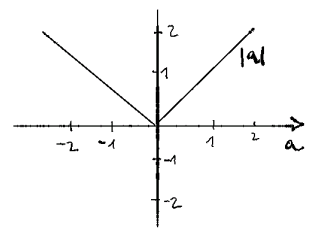
\includegraphics[width=0.4\textwidth]{betrag.png}
    \caption{Der Verlauf Funktion $f(x) =  x \, mod \, 4$.}
    \label{fig:modulo}
\end{figure}


% \bgInfo{
    Formaler ist die modulo Operation definiert als:
    $$ a{\bmod {m}}:=a-\left\lfloor {\frac {a}{m}}\right\rfloor \cdot m.$$
    Wobei die sog. Gaussklammern $\lfloor \cdot \rfloor$ hier für 'nach unten runden' (Engl. 'truncation') stehen. 

% }



% \begin{wrapfigure}{r}{0.4\textwidth}
%     \centering
%     %% Creator: Matplotlib, PGF backend
%%
%% To include the figure in your LaTeX document, write
%%   \input{<filename>.pgf}
%%
%% Make sure the required packages are loaded in your preamble
%%   \usepackage{pgf}
%%
%% Also ensure that all the required font packages are loaded; for instance,
%% the lmodern package is sometimes necessary when using math font.
%%   \usepackage{lmodern}
%%
%% Figures using additional raster images can only be included by \input if
%% they are in the same directory as the main LaTeX file. For loading figures
%% from other directories you can use the `import` package
%%   \usepackage{import}
%%
%% and then include the figures with
%%   \import{<path to file>}{<filename>.pgf}
%%
%% Matplotlib used the following preamble
%%   \def\mathdefault#1{#1}
%%   \everymath=\expandafter{\the\everymath\displaystyle}
%%   
%%   \usepackage{fontspec}
%%   \setmainfont{VeraSe.ttf}[Path=\detokenize{/usr/share/fonts/TTF/}]
%%   \setsansfont{DejaVuSans.ttf}[Path=\detokenize{/home/pl/miniconda3/lib/python3.12/site-packages/matplotlib/mpl-data/fonts/ttf/}]
%%   \setmonofont{DejaVuSansMono.ttf}[Path=\detokenize{/home/pl/miniconda3/lib/python3.12/site-packages/matplotlib/mpl-data/fonts/ttf/}]
%%   \makeatletter\@ifpackageloaded{underscore}{}{\usepackage[strings]{underscore}}\makeatother
%%
\begingroup%
\makeatletter%
\begin{pgfpicture}%
\pgfpathrectangle{\pgfpointorigin}{\pgfqpoint{2.710588in}{2.958486in}}%
\pgfusepath{use as bounding box, clip}%
\begin{pgfscope}%
\pgfsetbuttcap%
\pgfsetmiterjoin%
\definecolor{currentfill}{rgb}{1.000000,1.000000,1.000000}%
\pgfsetfillcolor{currentfill}%
\pgfsetlinewidth{0.000000pt}%
\definecolor{currentstroke}{rgb}{1.000000,1.000000,1.000000}%
\pgfsetstrokecolor{currentstroke}%
\pgfsetdash{}{0pt}%
\pgfpathmoveto{\pgfqpoint{0.000000in}{0.000000in}}%
\pgfpathlineto{\pgfqpoint{2.710588in}{0.000000in}}%
\pgfpathlineto{\pgfqpoint{2.710588in}{2.958486in}}%
\pgfpathlineto{\pgfqpoint{0.000000in}{2.958486in}}%
\pgfpathlineto{\pgfqpoint{0.000000in}{0.000000in}}%
\pgfpathclose%
\pgfusepath{fill}%
\end{pgfscope}%
\begin{pgfscope}%
\pgfsetbuttcap%
\pgfsetmiterjoin%
\definecolor{currentfill}{rgb}{1.000000,1.000000,1.000000}%
\pgfsetfillcolor{currentfill}%
\pgfsetlinewidth{0.000000pt}%
\definecolor{currentstroke}{rgb}{0.000000,0.000000,0.000000}%
\pgfsetstrokecolor{currentstroke}%
\pgfsetstrokeopacity{0.000000}%
\pgfsetdash{}{0pt}%
\pgfpathmoveto{\pgfqpoint{0.285587in}{0.548486in}}%
\pgfpathlineto{\pgfqpoint{2.610587in}{0.548486in}}%
\pgfpathlineto{\pgfqpoint{2.610587in}{2.858486in}}%
\pgfpathlineto{\pgfqpoint{0.285587in}{2.858486in}}%
\pgfpathlineto{\pgfqpoint{0.285587in}{0.548486in}}%
\pgfpathclose%
\pgfusepath{fill}%
\end{pgfscope}%
\begin{pgfscope}%
\pgfpathrectangle{\pgfqpoint{0.285587in}{0.548486in}}{\pgfqpoint{2.325000in}{2.310000in}}%
\pgfusepath{clip}%
\pgfsetrectcap%
\pgfsetroundjoin%
\pgfsetlinewidth{0.803000pt}%
\definecolor{currentstroke}{rgb}{0.690196,0.690196,0.690196}%
\pgfsetstrokecolor{currentstroke}%
\pgfsetdash{}{0pt}%
\pgfpathmoveto{\pgfqpoint{0.743542in}{0.548486in}}%
\pgfpathlineto{\pgfqpoint{0.743542in}{2.858486in}}%
\pgfusepath{stroke}%
\end{pgfscope}%
\begin{pgfscope}%
\pgfsetbuttcap%
\pgfsetroundjoin%
\definecolor{currentfill}{rgb}{0.000000,0.000000,0.000000}%
\pgfsetfillcolor{currentfill}%
\pgfsetlinewidth{0.803000pt}%
\definecolor{currentstroke}{rgb}{0.000000,0.000000,0.000000}%
\pgfsetstrokecolor{currentstroke}%
\pgfsetdash{}{0pt}%
\pgfsys@defobject{currentmarker}{\pgfqpoint{0.000000in}{-0.048611in}}{\pgfqpoint{0.000000in}{0.000000in}}{%
\pgfpathmoveto{\pgfqpoint{0.000000in}{0.000000in}}%
\pgfpathlineto{\pgfqpoint{0.000000in}{-0.048611in}}%
\pgfusepath{stroke,fill}%
}%
\begin{pgfscope}%
\pgfsys@transformshift{0.743542in}{0.548486in}%
\pgfsys@useobject{currentmarker}{}%
\end{pgfscope}%
\end{pgfscope}%
\begin{pgfscope}%
\definecolor{textcolor}{rgb}{0.000000,0.000000,0.000000}%
\pgfsetstrokecolor{textcolor}%
\pgfsetfillcolor{textcolor}%
\pgftext[x=0.743542in,y=0.451264in,,top]{\color{textcolor}{\rmfamily\fontsize{10.000000}{12.000000}\selectfont\catcode`\^=\active\def^{\ifmmode\sp\else\^{}\fi}\catcode`\%=\active\def%{\%}0}}%
\end{pgfscope}%
\begin{pgfscope}%
\pgfpathrectangle{\pgfqpoint{0.285587in}{0.548486in}}{\pgfqpoint{2.325000in}{2.310000in}}%
\pgfusepath{clip}%
\pgfsetrectcap%
\pgfsetroundjoin%
\pgfsetlinewidth{0.803000pt}%
\definecolor{currentstroke}{rgb}{0.690196,0.690196,0.690196}%
\pgfsetstrokecolor{currentstroke}%
\pgfsetdash{}{0pt}%
\pgfpathmoveto{\pgfqpoint{1.330663in}{0.548486in}}%
\pgfpathlineto{\pgfqpoint{1.330663in}{2.858486in}}%
\pgfusepath{stroke}%
\end{pgfscope}%
\begin{pgfscope}%
\pgfsetbuttcap%
\pgfsetroundjoin%
\definecolor{currentfill}{rgb}{0.000000,0.000000,0.000000}%
\pgfsetfillcolor{currentfill}%
\pgfsetlinewidth{0.803000pt}%
\definecolor{currentstroke}{rgb}{0.000000,0.000000,0.000000}%
\pgfsetstrokecolor{currentstroke}%
\pgfsetdash{}{0pt}%
\pgfsys@defobject{currentmarker}{\pgfqpoint{0.000000in}{-0.048611in}}{\pgfqpoint{0.000000in}{0.000000in}}{%
\pgfpathmoveto{\pgfqpoint{0.000000in}{0.000000in}}%
\pgfpathlineto{\pgfqpoint{0.000000in}{-0.048611in}}%
\pgfusepath{stroke,fill}%
}%
\begin{pgfscope}%
\pgfsys@transformshift{1.330663in}{0.548486in}%
\pgfsys@useobject{currentmarker}{}%
\end{pgfscope}%
\end{pgfscope}%
\begin{pgfscope}%
\definecolor{textcolor}{rgb}{0.000000,0.000000,0.000000}%
\pgfsetstrokecolor{textcolor}%
\pgfsetfillcolor{textcolor}%
\pgftext[x=1.330663in,y=0.451264in,,top]{\color{textcolor}{\rmfamily\fontsize{10.000000}{12.000000}\selectfont\catcode`\^=\active\def^{\ifmmode\sp\else\^{}\fi}\catcode`\%=\active\def%{\%}5}}%
\end{pgfscope}%
\begin{pgfscope}%
\pgfpathrectangle{\pgfqpoint{0.285587in}{0.548486in}}{\pgfqpoint{2.325000in}{2.310000in}}%
\pgfusepath{clip}%
\pgfsetrectcap%
\pgfsetroundjoin%
\pgfsetlinewidth{0.803000pt}%
\definecolor{currentstroke}{rgb}{0.690196,0.690196,0.690196}%
\pgfsetstrokecolor{currentstroke}%
\pgfsetdash{}{0pt}%
\pgfpathmoveto{\pgfqpoint{1.917784in}{0.548486in}}%
\pgfpathlineto{\pgfqpoint{1.917784in}{2.858486in}}%
\pgfusepath{stroke}%
\end{pgfscope}%
\begin{pgfscope}%
\pgfsetbuttcap%
\pgfsetroundjoin%
\definecolor{currentfill}{rgb}{0.000000,0.000000,0.000000}%
\pgfsetfillcolor{currentfill}%
\pgfsetlinewidth{0.803000pt}%
\definecolor{currentstroke}{rgb}{0.000000,0.000000,0.000000}%
\pgfsetstrokecolor{currentstroke}%
\pgfsetdash{}{0pt}%
\pgfsys@defobject{currentmarker}{\pgfqpoint{0.000000in}{-0.048611in}}{\pgfqpoint{0.000000in}{0.000000in}}{%
\pgfpathmoveto{\pgfqpoint{0.000000in}{0.000000in}}%
\pgfpathlineto{\pgfqpoint{0.000000in}{-0.048611in}}%
\pgfusepath{stroke,fill}%
}%
\begin{pgfscope}%
\pgfsys@transformshift{1.917784in}{0.548486in}%
\pgfsys@useobject{currentmarker}{}%
\end{pgfscope}%
\end{pgfscope}%
\begin{pgfscope}%
\definecolor{textcolor}{rgb}{0.000000,0.000000,0.000000}%
\pgfsetstrokecolor{textcolor}%
\pgfsetfillcolor{textcolor}%
\pgftext[x=1.917784in,y=0.451264in,,top]{\color{textcolor}{\rmfamily\fontsize{10.000000}{12.000000}\selectfont\catcode`\^=\active\def^{\ifmmode\sp\else\^{}\fi}\catcode`\%=\active\def%{\%}10}}%
\end{pgfscope}%
\begin{pgfscope}%
\pgfpathrectangle{\pgfqpoint{0.285587in}{0.548486in}}{\pgfqpoint{2.325000in}{2.310000in}}%
\pgfusepath{clip}%
\pgfsetrectcap%
\pgfsetroundjoin%
\pgfsetlinewidth{0.803000pt}%
\definecolor{currentstroke}{rgb}{0.690196,0.690196,0.690196}%
\pgfsetstrokecolor{currentstroke}%
\pgfsetdash{}{0pt}%
\pgfpathmoveto{\pgfqpoint{2.504906in}{0.548486in}}%
\pgfpathlineto{\pgfqpoint{2.504906in}{2.858486in}}%
\pgfusepath{stroke}%
\end{pgfscope}%
\begin{pgfscope}%
\pgfsetbuttcap%
\pgfsetroundjoin%
\definecolor{currentfill}{rgb}{0.000000,0.000000,0.000000}%
\pgfsetfillcolor{currentfill}%
\pgfsetlinewidth{0.803000pt}%
\definecolor{currentstroke}{rgb}{0.000000,0.000000,0.000000}%
\pgfsetstrokecolor{currentstroke}%
\pgfsetdash{}{0pt}%
\pgfsys@defobject{currentmarker}{\pgfqpoint{0.000000in}{-0.048611in}}{\pgfqpoint{0.000000in}{0.000000in}}{%
\pgfpathmoveto{\pgfqpoint{0.000000in}{0.000000in}}%
\pgfpathlineto{\pgfqpoint{0.000000in}{-0.048611in}}%
\pgfusepath{stroke,fill}%
}%
\begin{pgfscope}%
\pgfsys@transformshift{2.504906in}{0.548486in}%
\pgfsys@useobject{currentmarker}{}%
\end{pgfscope}%
\end{pgfscope}%
\begin{pgfscope}%
\definecolor{textcolor}{rgb}{0.000000,0.000000,0.000000}%
\pgfsetstrokecolor{textcolor}%
\pgfsetfillcolor{textcolor}%
\pgftext[x=2.504906in,y=0.451264in,,top]{\color{textcolor}{\rmfamily\fontsize{10.000000}{12.000000}\selectfont\catcode`\^=\active\def^{\ifmmode\sp\else\^{}\fi}\catcode`\%=\active\def%{\%}15}}%
\end{pgfscope}%
\begin{pgfscope}%
\definecolor{textcolor}{rgb}{0.000000,0.000000,0.000000}%
\pgfsetstrokecolor{textcolor}%
\pgfsetfillcolor{textcolor}%
\pgftext[x=1.448087in,y=0.261295in,,top]{\color{textcolor}{\rmfamily\fontsize{12.000000}{14.400000}\selectfont\catcode`\^=\active\def^{\ifmmode\sp\else\^{}\fi}\catcode`\%=\active\def%{\%}$x$}}%
\end{pgfscope}%
\begin{pgfscope}%
\pgfpathrectangle{\pgfqpoint{0.285587in}{0.548486in}}{\pgfqpoint{2.325000in}{2.310000in}}%
\pgfusepath{clip}%
\pgfsetrectcap%
\pgfsetroundjoin%
\pgfsetlinewidth{0.803000pt}%
\definecolor{currentstroke}{rgb}{0.690196,0.690196,0.690196}%
\pgfsetstrokecolor{currentstroke}%
\pgfsetdash{}{0pt}%
\pgfpathmoveto{\pgfqpoint{0.285587in}{0.648735in}}%
\pgfpathlineto{\pgfqpoint{2.610587in}{0.648735in}}%
\pgfusepath{stroke}%
\end{pgfscope}%
\begin{pgfscope}%
\pgfsetbuttcap%
\pgfsetroundjoin%
\definecolor{currentfill}{rgb}{0.000000,0.000000,0.000000}%
\pgfsetfillcolor{currentfill}%
\pgfsetlinewidth{0.803000pt}%
\definecolor{currentstroke}{rgb}{0.000000,0.000000,0.000000}%
\pgfsetstrokecolor{currentstroke}%
\pgfsetdash{}{0pt}%
\pgfsys@defobject{currentmarker}{\pgfqpoint{-0.048611in}{0.000000in}}{\pgfqpoint{-0.000000in}{0.000000in}}{%
\pgfpathmoveto{\pgfqpoint{-0.000000in}{0.000000in}}%
\pgfpathlineto{\pgfqpoint{-0.048611in}{0.000000in}}%
\pgfusepath{stroke,fill}%
}%
\begin{pgfscope}%
\pgfsys@transformshift{0.285587in}{0.648735in}%
\pgfsys@useobject{currentmarker}{}%
\end{pgfscope}%
\end{pgfscope}%
\begin{pgfscope}%
\definecolor{textcolor}{rgb}{0.000000,0.000000,0.000000}%
\pgfsetstrokecolor{textcolor}%
\pgfsetfillcolor{textcolor}%
\pgftext[x=0.100000in, y=0.595973in, left, base]{\color{textcolor}{\rmfamily\fontsize{10.000000}{12.000000}\selectfont\catcode`\^=\active\def^{\ifmmode\sp\else\^{}\fi}\catcode`\%=\active\def%{\%}0}}%
\end{pgfscope}%
\begin{pgfscope}%
\pgfpathrectangle{\pgfqpoint{0.285587in}{0.548486in}}{\pgfqpoint{2.325000in}{2.310000in}}%
\pgfusepath{clip}%
\pgfsetrectcap%
\pgfsetroundjoin%
\pgfsetlinewidth{0.803000pt}%
\definecolor{currentstroke}{rgb}{0.690196,0.690196,0.690196}%
\pgfsetstrokecolor{currentstroke}%
\pgfsetdash{}{0pt}%
\pgfpathmoveto{\pgfqpoint{0.285587in}{1.176110in}}%
\pgfpathlineto{\pgfqpoint{2.610587in}{1.176110in}}%
\pgfusepath{stroke}%
\end{pgfscope}%
\begin{pgfscope}%
\pgfsetbuttcap%
\pgfsetroundjoin%
\definecolor{currentfill}{rgb}{0.000000,0.000000,0.000000}%
\pgfsetfillcolor{currentfill}%
\pgfsetlinewidth{0.803000pt}%
\definecolor{currentstroke}{rgb}{0.000000,0.000000,0.000000}%
\pgfsetstrokecolor{currentstroke}%
\pgfsetdash{}{0pt}%
\pgfsys@defobject{currentmarker}{\pgfqpoint{-0.048611in}{0.000000in}}{\pgfqpoint{-0.000000in}{0.000000in}}{%
\pgfpathmoveto{\pgfqpoint{-0.000000in}{0.000000in}}%
\pgfpathlineto{\pgfqpoint{-0.048611in}{0.000000in}}%
\pgfusepath{stroke,fill}%
}%
\begin{pgfscope}%
\pgfsys@transformshift{0.285587in}{1.176110in}%
\pgfsys@useobject{currentmarker}{}%
\end{pgfscope}%
\end{pgfscope}%
\begin{pgfscope}%
\definecolor{textcolor}{rgb}{0.000000,0.000000,0.000000}%
\pgfsetstrokecolor{textcolor}%
\pgfsetfillcolor{textcolor}%
\pgftext[x=0.100000in, y=1.123349in, left, base]{\color{textcolor}{\rmfamily\fontsize{10.000000}{12.000000}\selectfont\catcode`\^=\active\def^{\ifmmode\sp\else\^{}\fi}\catcode`\%=\active\def%{\%}1}}%
\end{pgfscope}%
\begin{pgfscope}%
\pgfpathrectangle{\pgfqpoint{0.285587in}{0.548486in}}{\pgfqpoint{2.325000in}{2.310000in}}%
\pgfusepath{clip}%
\pgfsetrectcap%
\pgfsetroundjoin%
\pgfsetlinewidth{0.803000pt}%
\definecolor{currentstroke}{rgb}{0.690196,0.690196,0.690196}%
\pgfsetstrokecolor{currentstroke}%
\pgfsetdash{}{0pt}%
\pgfpathmoveto{\pgfqpoint{0.285587in}{1.703486in}}%
\pgfpathlineto{\pgfqpoint{2.610587in}{1.703486in}}%
\pgfusepath{stroke}%
\end{pgfscope}%
\begin{pgfscope}%
\pgfsetbuttcap%
\pgfsetroundjoin%
\definecolor{currentfill}{rgb}{0.000000,0.000000,0.000000}%
\pgfsetfillcolor{currentfill}%
\pgfsetlinewidth{0.803000pt}%
\definecolor{currentstroke}{rgb}{0.000000,0.000000,0.000000}%
\pgfsetstrokecolor{currentstroke}%
\pgfsetdash{}{0pt}%
\pgfsys@defobject{currentmarker}{\pgfqpoint{-0.048611in}{0.000000in}}{\pgfqpoint{-0.000000in}{0.000000in}}{%
\pgfpathmoveto{\pgfqpoint{-0.000000in}{0.000000in}}%
\pgfpathlineto{\pgfqpoint{-0.048611in}{0.000000in}}%
\pgfusepath{stroke,fill}%
}%
\begin{pgfscope}%
\pgfsys@transformshift{0.285587in}{1.703486in}%
\pgfsys@useobject{currentmarker}{}%
\end{pgfscope}%
\end{pgfscope}%
\begin{pgfscope}%
\definecolor{textcolor}{rgb}{0.000000,0.000000,0.000000}%
\pgfsetstrokecolor{textcolor}%
\pgfsetfillcolor{textcolor}%
\pgftext[x=0.100000in, y=1.650724in, left, base]{\color{textcolor}{\rmfamily\fontsize{10.000000}{12.000000}\selectfont\catcode`\^=\active\def^{\ifmmode\sp\else\^{}\fi}\catcode`\%=\active\def%{\%}2}}%
\end{pgfscope}%
\begin{pgfscope}%
\pgfpathrectangle{\pgfqpoint{0.285587in}{0.548486in}}{\pgfqpoint{2.325000in}{2.310000in}}%
\pgfusepath{clip}%
\pgfsetrectcap%
\pgfsetroundjoin%
\pgfsetlinewidth{0.803000pt}%
\definecolor{currentstroke}{rgb}{0.690196,0.690196,0.690196}%
\pgfsetstrokecolor{currentstroke}%
\pgfsetdash{}{0pt}%
\pgfpathmoveto{\pgfqpoint{0.285587in}{2.230862in}}%
\pgfpathlineto{\pgfqpoint{2.610587in}{2.230862in}}%
\pgfusepath{stroke}%
\end{pgfscope}%
\begin{pgfscope}%
\pgfsetbuttcap%
\pgfsetroundjoin%
\definecolor{currentfill}{rgb}{0.000000,0.000000,0.000000}%
\pgfsetfillcolor{currentfill}%
\pgfsetlinewidth{0.803000pt}%
\definecolor{currentstroke}{rgb}{0.000000,0.000000,0.000000}%
\pgfsetstrokecolor{currentstroke}%
\pgfsetdash{}{0pt}%
\pgfsys@defobject{currentmarker}{\pgfqpoint{-0.048611in}{0.000000in}}{\pgfqpoint{-0.000000in}{0.000000in}}{%
\pgfpathmoveto{\pgfqpoint{-0.000000in}{0.000000in}}%
\pgfpathlineto{\pgfqpoint{-0.048611in}{0.000000in}}%
\pgfusepath{stroke,fill}%
}%
\begin{pgfscope}%
\pgfsys@transformshift{0.285587in}{2.230862in}%
\pgfsys@useobject{currentmarker}{}%
\end{pgfscope}%
\end{pgfscope}%
\begin{pgfscope}%
\definecolor{textcolor}{rgb}{0.000000,0.000000,0.000000}%
\pgfsetstrokecolor{textcolor}%
\pgfsetfillcolor{textcolor}%
\pgftext[x=0.100000in, y=2.178100in, left, base]{\color{textcolor}{\rmfamily\fontsize{10.000000}{12.000000}\selectfont\catcode`\^=\active\def^{\ifmmode\sp\else\^{}\fi}\catcode`\%=\active\def%{\%}3}}%
\end{pgfscope}%
\begin{pgfscope}%
\pgfpathrectangle{\pgfqpoint{0.285587in}{0.548486in}}{\pgfqpoint{2.325000in}{2.310000in}}%
\pgfusepath{clip}%
\pgfsetrectcap%
\pgfsetroundjoin%
\pgfsetlinewidth{0.803000pt}%
\definecolor{currentstroke}{rgb}{0.690196,0.690196,0.690196}%
\pgfsetstrokecolor{currentstroke}%
\pgfsetdash{}{0pt}%
\pgfpathmoveto{\pgfqpoint{0.285587in}{2.758237in}}%
\pgfpathlineto{\pgfqpoint{2.610587in}{2.758237in}}%
\pgfusepath{stroke}%
\end{pgfscope}%
\begin{pgfscope}%
\pgfsetbuttcap%
\pgfsetroundjoin%
\definecolor{currentfill}{rgb}{0.000000,0.000000,0.000000}%
\pgfsetfillcolor{currentfill}%
\pgfsetlinewidth{0.803000pt}%
\definecolor{currentstroke}{rgb}{0.000000,0.000000,0.000000}%
\pgfsetstrokecolor{currentstroke}%
\pgfsetdash{}{0pt}%
\pgfsys@defobject{currentmarker}{\pgfqpoint{-0.048611in}{0.000000in}}{\pgfqpoint{-0.000000in}{0.000000in}}{%
\pgfpathmoveto{\pgfqpoint{-0.000000in}{0.000000in}}%
\pgfpathlineto{\pgfqpoint{-0.048611in}{0.000000in}}%
\pgfusepath{stroke,fill}%
}%
\begin{pgfscope}%
\pgfsys@transformshift{0.285587in}{2.758237in}%
\pgfsys@useobject{currentmarker}{}%
\end{pgfscope}%
\end{pgfscope}%
\begin{pgfscope}%
\definecolor{textcolor}{rgb}{0.000000,0.000000,0.000000}%
\pgfsetstrokecolor{textcolor}%
\pgfsetfillcolor{textcolor}%
\pgftext[x=0.100000in, y=2.705476in, left, base]{\color{textcolor}{\rmfamily\fontsize{10.000000}{12.000000}\selectfont\catcode`\^=\active\def^{\ifmmode\sp\else\^{}\fi}\catcode`\%=\active\def%{\%}4}}%
\end{pgfscope}%
\begin{pgfscope}%
\pgfpathrectangle{\pgfqpoint{0.285587in}{0.548486in}}{\pgfqpoint{2.325000in}{2.310000in}}%
\pgfusepath{clip}%
\pgfsetrectcap%
\pgfsetroundjoin%
\pgfsetlinewidth{1.505625pt}%
\definecolor{currentstroke}{rgb}{0.000000,0.000000,0.000000}%
\pgfsetstrokecolor{currentstroke}%
\pgfsetdash{}{0pt}%
\pgfpathmoveto{\pgfqpoint{0.391269in}{1.176110in}}%
\pgfpathlineto{\pgfqpoint{0.742484in}{2.753486in}}%
\pgfpathlineto{\pgfqpoint{0.744600in}{0.653486in}}%
\pgfpathlineto{\pgfqpoint{1.212181in}{2.753486in}}%
\pgfpathlineto{\pgfqpoint{1.214297in}{0.653486in}}%
\pgfpathlineto{\pgfqpoint{1.681878in}{2.753486in}}%
\pgfpathlineto{\pgfqpoint{1.683994in}{0.653486in}}%
\pgfpathlineto{\pgfqpoint{2.151575in}{2.753486in}}%
\pgfpathlineto{\pgfqpoint{2.153691in}{0.653486in}}%
\pgfpathlineto{\pgfqpoint{2.504906in}{2.230862in}}%
\pgfpathlineto{\pgfqpoint{2.504906in}{2.230862in}}%
\pgfusepath{stroke}%
\end{pgfscope}%
\begin{pgfscope}%
\pgfpathrectangle{\pgfqpoint{0.285587in}{0.548486in}}{\pgfqpoint{2.325000in}{2.310000in}}%
\pgfusepath{clip}%
\pgfsetrectcap%
\pgfsetroundjoin%
\pgfsetlinewidth{0.501875pt}%
\definecolor{currentstroke}{rgb}{0.000000,0.000000,0.000000}%
\pgfsetstrokecolor{currentstroke}%
\pgfsetdash{}{0pt}%
\pgfpathmoveto{\pgfqpoint{0.285587in}{0.648735in}}%
\pgfpathlineto{\pgfqpoint{2.610587in}{0.648735in}}%
\pgfusepath{stroke}%
\end{pgfscope}%
\begin{pgfscope}%
\pgfpathrectangle{\pgfqpoint{0.285587in}{0.548486in}}{\pgfqpoint{2.325000in}{2.310000in}}%
\pgfusepath{clip}%
\pgfsetrectcap%
\pgfsetroundjoin%
\pgfsetlinewidth{0.501875pt}%
\definecolor{currentstroke}{rgb}{0.000000,0.000000,0.000000}%
\pgfsetstrokecolor{currentstroke}%
\pgfsetdash{}{0pt}%
\pgfpathmoveto{\pgfqpoint{0.743542in}{0.548486in}}%
\pgfpathlineto{\pgfqpoint{0.743542in}{2.858486in}}%
\pgfusepath{stroke}%
\end{pgfscope}%
\end{pgfpicture}%
\makeatother%
\endgroup%

%     \caption{An example figure}
% \end{wrapfigure}

\subsection{Summe und Produkt Notation}

Das große Sigma, $\Sigma$ ist eine kurzschreibweise für Summen. Wir finden dieses Zeichen oft in Blockdiagrammen um eine Addition zu verdeutlichen und manchmal sogar auf Mischpulten als Zier in der Gegend der 'Summe'/des Master Faders. Es handelt sich um eine simple Addition, also nichts was zu Irritation führen sollte. In der Praxis kann es allerdings vorkommen, dass sich vor allem bei unendlichen Summen einige Komplexität hinter so einer Summe verbirgt. Die Notation alleine sollte aber nicht abschrecken:

\begin{equation}
{\displaystyle \sum _{k=1}^{5}k = 1 + 2 + 3 + 4 + 5 }
\end{equation}
\index{Index}
Hier ist $k$ der \emph{Index} (Auch 'Laufindex' oder 'Zähler' genannt). Unter dem Sigma steht bei welcher zahl zu zählen begonnen wird und welchen Buchstaben wir als Index wählen. über dem Sigma steht bis wohin wir zählen. Nach dem Sigma steht was addiert wird. Allgemein:

\important{
\begin{equation}
{\displaystyle \sum _{k=m}^{n}a_{k}=\sum _{m\leq k\leq n}a_{k}=a_{m}+a_{m+1}+\dotsb +a_{n}.}
\end{equation}
}


Natürlich kann diese Schreibweise verwendet werden um kompliziertere Ausdrücke zu formen.

\begin{question}
Schreiben Sie einen Ausdruck der die \textbf{geraden} Zahlen zwischen 0 und 11 quadriert und addiert!
\end{question}
\begin{answer}

$${\displaystyle \sum _{k=0}^{5} (k \cdot 2)^2 = 0 + (1 \cdot 2)^2 + (2 \cdot 2)^2 + (3 \cdot 2)^2 + (4 \cdot 2)^2 + (5 \cdot 2)^2}$$

\end{answer}


\praxis{Im Audio Bereich finden wir Summenzeichen in vielen Bereichen. Bei der Diskreten Fourier Transformation, bei Filtern, bei der Beschreibung des Zusammenmischens vieler Signale im Allgemeinen (egal ob elektrisch oder akustisch), bei 'Discrete Summation Formula'(DSF)-Synthese und in vielen anderen Bereichen.}


% \todo[]{summe erklärungen, beispiel. Praxisbezug. Beschreibung des ausgangssignals bei einem Mixer, DSF synthesis, diskrete fourier transf. }

% \todo[]{prod. Beispiel filter Kaskadieren (produkte)}

Die Notation für Produkte trifft man nicht ganz so oft an wie jene für Summen:

\begin{equation}
{\displaystyle \prod _{i=1}^{6}i^{2} =  1\cdot 4\cdot 9\cdot 16\cdot 25\cdot 36}
\end{equation}

Im Audio Bereich ist natürlich auch diese Notation wichtig (Multiplikation ist eine wichtige Operation). Ein Beispiel wäre, gegeben einen Filter mit der Transferfunktion $H$ könnte man $n$ hintereinander geschaltene ('kaskadierte') Filter schreiben als $\prod _{i=1}^{n}H$.


\subsection{Betrag}

% \begin{wrapfigure}{r}{0.4\textwidth}
%     \centering
%     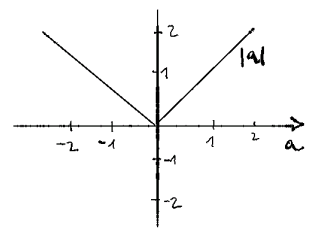
\includegraphics[width=0.4\textwidth]{betrag.png}
%     \caption{Betrag als Input/Output Plot.}
%     \label{fig:betrag}
% \end{wrapfigure}

Der Betrag macht alles positiv. Der \emph{Betrag} einer Zahl $a \in \mathbb{R}$, dargestellt als $|a|$ kann folgendermaßen definiert werden:
$$ 
|a| \coloneqq
\begin{cases} 
-a & \text{wenn } a < 0 \\ 
a & \text{wenn } a \geq 0 
\end{cases}
$$ 

Der Betrag kann als \emph{Funktion} aufgefasst werden (später mehr zu Funktionen). Es Kann ein Graph gezeichnet werden auf dessen x-Achse ('Abszisse') der Input zu sehen ist und auf der y-Achse ('Ordinate'). Merkhilfe: Alphabetisch: x vor y, Abszisse vor Ordinate.



\begin{figure}[h!]
    \centering
    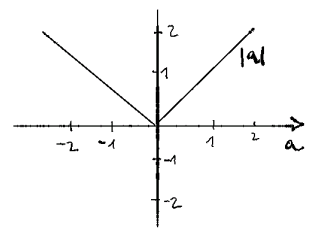
\includegraphics[width=0.4\textwidth]{betrag.png}
    \caption{Betrag als Input/Output Plot.}
    \label{fig:betrag}
\end{figure}

\index{Betrag}
\index{Absolutwert}

\praxis{
Der Betrag (oder auch Absolutwert) hat in der Audio Technik eine Wichtige Rolle, speziell der Betrag von Komplexen Zahlen, den Ergebnissen der Fourier Transformation. In der Elektrotechnik kann er als 'Gleichrichter' gefunden werden um Wechselströme zu Gleichströmen zu wandeln. Er ist eine der simpelsten Verzerrungen mit geraden harmonischen.
}

Soundbeispiel hier: \faust{Betrag Einer 150Hz Sinus Schwingung}{https://faustide.grame.fr/?autorun=1\&voices=0\&name=abs_test\&inline=aW1wb3J0KCJzdGRmYXVzdC5saWIiKTsKcHJvY2VzcyA9IG9zLm9zYygxNTApOmFiczs\%3D}

\begin{figure}[H]
    \centering
    %% Creator: Matplotlib, PGF backend
%%
%% To include the figure in your LaTeX document, write
%%   \input{<filename>.pgf}
%%
%% Make sure the required packages are loaded in your preamble
%%   \usepackage{pgf}
%%
%% Also ensure that all the required font packages are loaded; for instance,
%% the lmodern package is sometimes necessary when using math font.
%%   \usepackage{lmodern}
%%
%% Figures using additional raster images can only be included by \input if
%% they are in the same directory as the main LaTeX file. For loading figures
%% from other directories you can use the `import` package
%%   \usepackage{import}
%%
%% and then include the figures with
%%   \import{<path to file>}{<filename>.pgf}
%%
%% Matplotlib used the following preamble
%%   \def\mathdefault#1{#1}
%%   \everymath=\expandafter{\the\everymath\displaystyle}
%%   
%%   \usepackage{fontspec}
%%   \setmainfont{VeraSe.ttf}[Path=\detokenize{/usr/share/fonts/TTF/}]
%%   \setsansfont{DejaVuSans.ttf}[Path=\detokenize{/home/pl/miniconda3/lib/python3.12/site-packages/matplotlib/mpl-data/fonts/ttf/}]
%%   \setmonofont{DejaVuSansMono.ttf}[Path=\detokenize{/home/pl/miniconda3/lib/python3.12/site-packages/matplotlib/mpl-data/fonts/ttf/}]
%%   \makeatletter\@ifpackageloaded{underscore}{}{\usepackage[strings]{underscore}}\makeatother
%%
\begingroup%
\makeatletter%
\begin{pgfpicture}%
\pgfpathrectangle{\pgfpointorigin}{\pgfqpoint{5.276127in}{1.740000in}}%
\pgfusepath{use as bounding box, clip}%
\begin{pgfscope}%
\pgfsetbuttcap%
\pgfsetmiterjoin%
\definecolor{currentfill}{rgb}{1.000000,1.000000,1.000000}%
\pgfsetfillcolor{currentfill}%
\pgfsetlinewidth{0.000000pt}%
\definecolor{currentstroke}{rgb}{1.000000,1.000000,1.000000}%
\pgfsetstrokecolor{currentstroke}%
\pgfsetdash{}{0pt}%
\pgfpathmoveto{\pgfqpoint{0.000000in}{0.000000in}}%
\pgfpathlineto{\pgfqpoint{5.276127in}{0.000000in}}%
\pgfpathlineto{\pgfqpoint{5.276127in}{1.740000in}}%
\pgfpathlineto{\pgfqpoint{0.000000in}{1.740000in}}%
\pgfpathlineto{\pgfqpoint{0.000000in}{0.000000in}}%
\pgfpathclose%
\pgfusepath{fill}%
\end{pgfscope}%
\begin{pgfscope}%
\pgfsetbuttcap%
\pgfsetmiterjoin%
\definecolor{currentfill}{rgb}{1.000000,1.000000,1.000000}%
\pgfsetfillcolor{currentfill}%
\pgfsetlinewidth{0.000000pt}%
\definecolor{currentstroke}{rgb}{0.000000,0.000000,0.000000}%
\pgfsetstrokecolor{currentstroke}%
\pgfsetstrokeopacity{0.000000}%
\pgfsetdash{}{0pt}%
\pgfpathmoveto{\pgfqpoint{0.526127in}{0.100000in}}%
\pgfpathlineto{\pgfqpoint{2.639763in}{0.100000in}}%
\pgfpathlineto{\pgfqpoint{2.639763in}{1.640000in}}%
\pgfpathlineto{\pgfqpoint{0.526127in}{1.640000in}}%
\pgfpathlineto{\pgfqpoint{0.526127in}{0.100000in}}%
\pgfpathclose%
\pgfusepath{fill}%
\end{pgfscope}%
\begin{pgfscope}%
\pgfsetbuttcap%
\pgfsetroundjoin%
\definecolor{currentfill}{rgb}{0.000000,0.000000,0.000000}%
\pgfsetfillcolor{currentfill}%
\pgfsetlinewidth{0.803000pt}%
\definecolor{currentstroke}{rgb}{0.000000,0.000000,0.000000}%
\pgfsetstrokecolor{currentstroke}%
\pgfsetdash{}{0pt}%
\pgfsys@defobject{currentmarker}{\pgfqpoint{-0.048611in}{0.000000in}}{\pgfqpoint{-0.000000in}{0.000000in}}{%
\pgfpathmoveto{\pgfqpoint{-0.000000in}{0.000000in}}%
\pgfpathlineto{\pgfqpoint{-0.048611in}{0.000000in}}%
\pgfusepath{stroke,fill}%
}%
\begin{pgfscope}%
\pgfsys@transformshift{0.526127in}{0.228333in}%
\pgfsys@useobject{currentmarker}{}%
\end{pgfscope}%
\end{pgfscope}%
\begin{pgfscope}%
\definecolor{textcolor}{rgb}{0.000000,0.000000,0.000000}%
\pgfsetstrokecolor{textcolor}%
\pgfsetfillcolor{textcolor}%
\pgftext[x=0.100000in, y=0.175572in, left, base]{\color{textcolor}{\rmfamily\fontsize{10.000000}{12.000000}\selectfont\catcode`\^=\active\def^{\ifmmode\sp\else\^{}\fi}\catcode`\%=\active\def%{\%}\ensuremath{-}1.0}}%
\end{pgfscope}%
\begin{pgfscope}%
\pgfsetbuttcap%
\pgfsetroundjoin%
\definecolor{currentfill}{rgb}{0.000000,0.000000,0.000000}%
\pgfsetfillcolor{currentfill}%
\pgfsetlinewidth{0.803000pt}%
\definecolor{currentstroke}{rgb}{0.000000,0.000000,0.000000}%
\pgfsetstrokecolor{currentstroke}%
\pgfsetdash{}{0pt}%
\pgfsys@defobject{currentmarker}{\pgfqpoint{-0.048611in}{0.000000in}}{\pgfqpoint{-0.000000in}{0.000000in}}{%
\pgfpathmoveto{\pgfqpoint{-0.000000in}{0.000000in}}%
\pgfpathlineto{\pgfqpoint{-0.048611in}{0.000000in}}%
\pgfusepath{stroke,fill}%
}%
\begin{pgfscope}%
\pgfsys@transformshift{0.526127in}{0.549167in}%
\pgfsys@useobject{currentmarker}{}%
\end{pgfscope}%
\end{pgfscope}%
\begin{pgfscope}%
\definecolor{textcolor}{rgb}{0.000000,0.000000,0.000000}%
\pgfsetstrokecolor{textcolor}%
\pgfsetfillcolor{textcolor}%
\pgftext[x=0.100000in, y=0.496405in, left, base]{\color{textcolor}{\rmfamily\fontsize{10.000000}{12.000000}\selectfont\catcode`\^=\active\def^{\ifmmode\sp\else\^{}\fi}\catcode`\%=\active\def%{\%}\ensuremath{-}0.5}}%
\end{pgfscope}%
\begin{pgfscope}%
\pgfsetbuttcap%
\pgfsetroundjoin%
\definecolor{currentfill}{rgb}{0.000000,0.000000,0.000000}%
\pgfsetfillcolor{currentfill}%
\pgfsetlinewidth{0.803000pt}%
\definecolor{currentstroke}{rgb}{0.000000,0.000000,0.000000}%
\pgfsetstrokecolor{currentstroke}%
\pgfsetdash{}{0pt}%
\pgfsys@defobject{currentmarker}{\pgfqpoint{-0.048611in}{0.000000in}}{\pgfqpoint{-0.000000in}{0.000000in}}{%
\pgfpathmoveto{\pgfqpoint{-0.000000in}{0.000000in}}%
\pgfpathlineto{\pgfqpoint{-0.048611in}{0.000000in}}%
\pgfusepath{stroke,fill}%
}%
\begin{pgfscope}%
\pgfsys@transformshift{0.526127in}{0.870000in}%
\pgfsys@useobject{currentmarker}{}%
\end{pgfscope}%
\end{pgfscope}%
\begin{pgfscope}%
\definecolor{textcolor}{rgb}{0.000000,0.000000,0.000000}%
\pgfsetstrokecolor{textcolor}%
\pgfsetfillcolor{textcolor}%
\pgftext[x=0.208025in, y=0.817238in, left, base]{\color{textcolor}{\rmfamily\fontsize{10.000000}{12.000000}\selectfont\catcode`\^=\active\def^{\ifmmode\sp\else\^{}\fi}\catcode`\%=\active\def%{\%}0.0}}%
\end{pgfscope}%
\begin{pgfscope}%
\pgfsetbuttcap%
\pgfsetroundjoin%
\definecolor{currentfill}{rgb}{0.000000,0.000000,0.000000}%
\pgfsetfillcolor{currentfill}%
\pgfsetlinewidth{0.803000pt}%
\definecolor{currentstroke}{rgb}{0.000000,0.000000,0.000000}%
\pgfsetstrokecolor{currentstroke}%
\pgfsetdash{}{0pt}%
\pgfsys@defobject{currentmarker}{\pgfqpoint{-0.048611in}{0.000000in}}{\pgfqpoint{-0.000000in}{0.000000in}}{%
\pgfpathmoveto{\pgfqpoint{-0.000000in}{0.000000in}}%
\pgfpathlineto{\pgfqpoint{-0.048611in}{0.000000in}}%
\pgfusepath{stroke,fill}%
}%
\begin{pgfscope}%
\pgfsys@transformshift{0.526127in}{1.190833in}%
\pgfsys@useobject{currentmarker}{}%
\end{pgfscope}%
\end{pgfscope}%
\begin{pgfscope}%
\definecolor{textcolor}{rgb}{0.000000,0.000000,0.000000}%
\pgfsetstrokecolor{textcolor}%
\pgfsetfillcolor{textcolor}%
\pgftext[x=0.208025in, y=1.138072in, left, base]{\color{textcolor}{\rmfamily\fontsize{10.000000}{12.000000}\selectfont\catcode`\^=\active\def^{\ifmmode\sp\else\^{}\fi}\catcode`\%=\active\def%{\%}0.5}}%
\end{pgfscope}%
\begin{pgfscope}%
\pgfsetbuttcap%
\pgfsetroundjoin%
\definecolor{currentfill}{rgb}{0.000000,0.000000,0.000000}%
\pgfsetfillcolor{currentfill}%
\pgfsetlinewidth{0.803000pt}%
\definecolor{currentstroke}{rgb}{0.000000,0.000000,0.000000}%
\pgfsetstrokecolor{currentstroke}%
\pgfsetdash{}{0pt}%
\pgfsys@defobject{currentmarker}{\pgfqpoint{-0.048611in}{0.000000in}}{\pgfqpoint{-0.000000in}{0.000000in}}{%
\pgfpathmoveto{\pgfqpoint{-0.000000in}{0.000000in}}%
\pgfpathlineto{\pgfqpoint{-0.048611in}{0.000000in}}%
\pgfusepath{stroke,fill}%
}%
\begin{pgfscope}%
\pgfsys@transformshift{0.526127in}{1.511667in}%
\pgfsys@useobject{currentmarker}{}%
\end{pgfscope}%
\end{pgfscope}%
\begin{pgfscope}%
\definecolor{textcolor}{rgb}{0.000000,0.000000,0.000000}%
\pgfsetstrokecolor{textcolor}%
\pgfsetfillcolor{textcolor}%
\pgftext[x=0.208025in, y=1.458905in, left, base]{\color{textcolor}{\rmfamily\fontsize{10.000000}{12.000000}\selectfont\catcode`\^=\active\def^{\ifmmode\sp\else\^{}\fi}\catcode`\%=\active\def%{\%}1.0}}%
\end{pgfscope}%
\begin{pgfscope}%
\pgfpathrectangle{\pgfqpoint{0.526127in}{0.100000in}}{\pgfqpoint{2.113636in}{1.540000in}}%
\pgfusepath{clip}%
\pgfsetrectcap%
\pgfsetroundjoin%
\pgfsetlinewidth{1.505625pt}%
\definecolor{currentstroke}{rgb}{0.000000,0.000000,0.000000}%
\pgfsetstrokecolor{currentstroke}%
\pgfsetdash{}{0pt}%
\pgfpathmoveto{\pgfqpoint{0.622201in}{0.870000in}}%
\pgfpathlineto{\pgfqpoint{0.717208in}{0.968077in}}%
\pgfpathlineto{\pgfqpoint{0.767762in}{1.017008in}}%
\pgfpathlineto{\pgfqpoint{0.810035in}{1.054901in}}%
\pgfpathlineto{\pgfqpoint{0.847515in}{1.085567in}}%
\pgfpathlineto{\pgfqpoint{0.881944in}{1.110898in}}%
\pgfpathlineto{\pgfqpoint{0.913758in}{1.131600in}}%
\pgfpathlineto{\pgfqpoint{0.943829in}{1.148571in}}%
\pgfpathlineto{\pgfqpoint{0.972593in}{1.162288in}}%
\pgfpathlineto{\pgfqpoint{1.000049in}{1.172972in}}%
\pgfpathlineto{\pgfqpoint{1.027069in}{1.181104in}}%
\pgfpathlineto{\pgfqpoint{1.053217in}{1.186664in}}%
\pgfpathlineto{\pgfqpoint{1.078930in}{1.189875in}}%
\pgfpathlineto{\pgfqpoint{1.104643in}{1.190826in}}%
\pgfpathlineto{\pgfqpoint{1.129920in}{1.189551in}}%
\pgfpathlineto{\pgfqpoint{1.155633in}{1.186016in}}%
\pgfpathlineto{\pgfqpoint{1.181346in}{1.180249in}}%
\pgfpathlineto{\pgfqpoint{1.207930in}{1.171981in}}%
\pgfpathlineto{\pgfqpoint{1.234950in}{1.161242in}}%
\pgfpathlineto{\pgfqpoint{1.263278in}{1.147545in}}%
\pgfpathlineto{\pgfqpoint{1.292477in}{1.130937in}}%
\pgfpathlineto{\pgfqpoint{1.323420in}{1.110747in}}%
\pgfpathlineto{\pgfqpoint{1.356541in}{1.086412in}}%
\pgfpathlineto{\pgfqpoint{1.392278in}{1.057321in}}%
\pgfpathlineto{\pgfqpoint{1.431501in}{1.022467in}}%
\pgfpathlineto{\pgfqpoint{1.476825in}{0.979111in}}%
\pgfpathlineto{\pgfqpoint{1.533916in}{0.921216in}}%
\pgfpathlineto{\pgfqpoint{1.708676in}{0.741779in}}%
\pgfpathlineto{\pgfqpoint{1.753565in}{0.700144in}}%
\pgfpathlineto{\pgfqpoint{1.792788in}{0.666725in}}%
\pgfpathlineto{\pgfqpoint{1.828088in}{0.639489in}}%
\pgfpathlineto{\pgfqpoint{1.860774in}{0.616999in}}%
\pgfpathlineto{\pgfqpoint{1.891716in}{0.598364in}}%
\pgfpathlineto{\pgfqpoint{1.920916in}{0.583325in}}%
\pgfpathlineto{\pgfqpoint{1.948808in}{0.571396in}}%
\pgfpathlineto{\pgfqpoint{1.975828in}{0.562207in}}%
\pgfpathlineto{\pgfqpoint{2.002412in}{0.555508in}}%
\pgfpathlineto{\pgfqpoint{2.028125in}{0.551289in}}%
\pgfpathlineto{\pgfqpoint{2.053838in}{0.549321in}}%
\pgfpathlineto{\pgfqpoint{2.079115in}{0.549595in}}%
\pgfpathlineto{\pgfqpoint{2.104828in}{0.552118in}}%
\pgfpathlineto{\pgfqpoint{2.130540in}{0.556887in}}%
\pgfpathlineto{\pgfqpoint{2.156689in}{0.564005in}}%
\pgfpathlineto{\pgfqpoint{2.183709in}{0.573709in}}%
\pgfpathlineto{\pgfqpoint{2.211601in}{0.586149in}}%
\pgfpathlineto{\pgfqpoint{2.240365in}{0.601449in}}%
\pgfpathlineto{\pgfqpoint{2.270436in}{0.619979in}}%
\pgfpathlineto{\pgfqpoint{2.302250in}{0.642209in}}%
\pgfpathlineto{\pgfqpoint{2.336679in}{0.669033in}}%
\pgfpathlineto{\pgfqpoint{2.374158in}{0.701114in}}%
\pgfpathlineto{\pgfqpoint{2.416432in}{0.740313in}}%
\pgfpathlineto{\pgfqpoint{2.466986in}{0.790371in}}%
\pgfpathlineto{\pgfqpoint{2.541074in}{0.867257in}}%
\pgfpathlineto{\pgfqpoint{2.543689in}{0.870000in}}%
\pgfpathlineto{\pgfqpoint{2.543689in}{0.870000in}}%
\pgfusepath{stroke}%
\end{pgfscope}%
\begin{pgfscope}%
\pgfpathrectangle{\pgfqpoint{0.526127in}{0.100000in}}{\pgfqpoint{2.113636in}{1.540000in}}%
\pgfusepath{clip}%
\pgfsetbuttcap%
\pgfsetroundjoin%
\pgfsetlinewidth{1.505625pt}%
\definecolor{currentstroke}{rgb}{1.000000,0.000000,0.000000}%
\pgfsetstrokecolor{currentstroke}%
\pgfsetdash{{5.550000pt}{2.400000pt}}{0.000000pt}%
\pgfpathmoveto{\pgfqpoint{0.622201in}{0.870000in}}%
\pgfpathlineto{\pgfqpoint{0.717208in}{0.968077in}}%
\pgfpathlineto{\pgfqpoint{0.767762in}{1.017008in}}%
\pgfpathlineto{\pgfqpoint{0.810035in}{1.054901in}}%
\pgfpathlineto{\pgfqpoint{0.847515in}{1.085567in}}%
\pgfpathlineto{\pgfqpoint{0.881944in}{1.110898in}}%
\pgfpathlineto{\pgfqpoint{0.913758in}{1.131600in}}%
\pgfpathlineto{\pgfqpoint{0.943829in}{1.148571in}}%
\pgfpathlineto{\pgfqpoint{0.972593in}{1.162288in}}%
\pgfpathlineto{\pgfqpoint{1.000049in}{1.172972in}}%
\pgfpathlineto{\pgfqpoint{1.027069in}{1.181104in}}%
\pgfpathlineto{\pgfqpoint{1.053217in}{1.186664in}}%
\pgfpathlineto{\pgfqpoint{1.078930in}{1.189875in}}%
\pgfpathlineto{\pgfqpoint{1.104643in}{1.190826in}}%
\pgfpathlineto{\pgfqpoint{1.129920in}{1.189551in}}%
\pgfpathlineto{\pgfqpoint{1.155633in}{1.186016in}}%
\pgfpathlineto{\pgfqpoint{1.181346in}{1.180249in}}%
\pgfpathlineto{\pgfqpoint{1.207930in}{1.171981in}}%
\pgfpathlineto{\pgfqpoint{1.234950in}{1.161242in}}%
\pgfpathlineto{\pgfqpoint{1.263278in}{1.147545in}}%
\pgfpathlineto{\pgfqpoint{1.292477in}{1.130937in}}%
\pgfpathlineto{\pgfqpoint{1.323420in}{1.110747in}}%
\pgfpathlineto{\pgfqpoint{1.356541in}{1.086412in}}%
\pgfpathlineto{\pgfqpoint{1.392278in}{1.057321in}}%
\pgfpathlineto{\pgfqpoint{1.431501in}{1.022467in}}%
\pgfpathlineto{\pgfqpoint{1.476825in}{0.979111in}}%
\pgfpathlineto{\pgfqpoint{1.533916in}{0.921216in}}%
\pgfpathlineto{\pgfqpoint{1.583163in}{0.870229in}}%
\pgfpathlineto{\pgfqpoint{1.583599in}{0.870686in}}%
\pgfpathlineto{\pgfqpoint{1.678169in}{0.968295in}}%
\pgfpathlineto{\pgfqpoint{1.728723in}{1.017211in}}%
\pgfpathlineto{\pgfqpoint{1.770997in}{1.055087in}}%
\pgfpathlineto{\pgfqpoint{1.808477in}{1.085736in}}%
\pgfpathlineto{\pgfqpoint{1.842906in}{1.111049in}}%
\pgfpathlineto{\pgfqpoint{1.874720in}{1.131732in}}%
\pgfpathlineto{\pgfqpoint{1.904791in}{1.148684in}}%
\pgfpathlineto{\pgfqpoint{1.933554in}{1.162382in}}%
\pgfpathlineto{\pgfqpoint{1.961010in}{1.173047in}}%
\pgfpathlineto{\pgfqpoint{1.987595in}{1.181048in}}%
\pgfpathlineto{\pgfqpoint{2.013743in}{1.186627in}}%
\pgfpathlineto{\pgfqpoint{2.039456in}{1.189857in}}%
\pgfpathlineto{\pgfqpoint{2.065169in}{1.190827in}}%
\pgfpathlineto{\pgfqpoint{2.090446in}{1.189572in}}%
\pgfpathlineto{\pgfqpoint{2.116159in}{1.186056in}}%
\pgfpathlineto{\pgfqpoint{2.141872in}{1.180307in}}%
\pgfpathlineto{\pgfqpoint{2.168456in}{1.172058in}}%
\pgfpathlineto{\pgfqpoint{2.195476in}{1.161337in}}%
\pgfpathlineto{\pgfqpoint{2.223804in}{1.147659in}}%
\pgfpathlineto{\pgfqpoint{2.253003in}{1.131070in}}%
\pgfpathlineto{\pgfqpoint{2.283946in}{1.110898in}}%
\pgfpathlineto{\pgfqpoint{2.317067in}{1.086581in}}%
\pgfpathlineto{\pgfqpoint{2.352804in}{1.057507in}}%
\pgfpathlineto{\pgfqpoint{2.392027in}{1.022668in}}%
\pgfpathlineto{\pgfqpoint{2.437351in}{0.979326in}}%
\pgfpathlineto{\pgfqpoint{2.494442in}{0.921442in}}%
\pgfpathlineto{\pgfqpoint{2.543689in}{0.870000in}}%
\pgfpathlineto{\pgfqpoint{2.543689in}{0.870000in}}%
\pgfusepath{stroke}%
\end{pgfscope}%
\begin{pgfscope}%
\pgfpathrectangle{\pgfqpoint{0.526127in}{0.100000in}}{\pgfqpoint{2.113636in}{1.540000in}}%
\pgfusepath{clip}%
\pgfsetrectcap%
\pgfsetroundjoin%
\pgfsetlinewidth{0.501875pt}%
\definecolor{currentstroke}{rgb}{0.000000,0.000000,0.000000}%
\pgfsetstrokecolor{currentstroke}%
\pgfsetdash{}{0pt}%
\pgfpathmoveto{\pgfqpoint{0.526127in}{0.870000in}}%
\pgfpathlineto{\pgfqpoint{2.639763in}{0.870000in}}%
\pgfusepath{stroke}%
\end{pgfscope}%
\begin{pgfscope}%
\pgfsetbuttcap%
\pgfsetmiterjoin%
\definecolor{currentfill}{rgb}{1.000000,1.000000,1.000000}%
\pgfsetfillcolor{currentfill}%
\pgfsetfillopacity{0.800000}%
\pgfsetlinewidth{1.003750pt}%
\definecolor{currentstroke}{rgb}{0.800000,0.800000,0.800000}%
\pgfsetstrokecolor{currentstroke}%
\pgfsetstrokeopacity{0.800000}%
\pgfsetdash{}{0pt}%
\pgfpathmoveto{\pgfqpoint{0.623349in}{0.169444in}}%
\pgfpathlineto{\pgfqpoint{1.376549in}{0.169444in}}%
\pgfpathquadraticcurveto{\pgfqpoint{1.404326in}{0.169444in}}{\pgfqpoint{1.404326in}{0.197222in}}%
\pgfpathlineto{\pgfqpoint{1.404326in}{0.602713in}}%
\pgfpathquadraticcurveto{\pgfqpoint{1.404326in}{0.630491in}}{\pgfqpoint{1.376549in}{0.630491in}}%
\pgfpathlineto{\pgfqpoint{0.623349in}{0.630491in}}%
\pgfpathquadraticcurveto{\pgfqpoint{0.595571in}{0.630491in}}{\pgfqpoint{0.595571in}{0.602713in}}%
\pgfpathlineto{\pgfqpoint{0.595571in}{0.197222in}}%
\pgfpathquadraticcurveto{\pgfqpoint{0.595571in}{0.169444in}}{\pgfqpoint{0.623349in}{0.169444in}}%
\pgfpathlineto{\pgfqpoint{0.623349in}{0.169444in}}%
\pgfpathclose%
\pgfusepath{stroke,fill}%
\end{pgfscope}%
\begin{pgfscope}%
\pgfsetrectcap%
\pgfsetroundjoin%
\pgfsetlinewidth{1.505625pt}%
\definecolor{currentstroke}{rgb}{0.000000,0.000000,0.000000}%
\pgfsetstrokecolor{currentstroke}%
\pgfsetdash{}{0pt}%
\pgfpathmoveto{\pgfqpoint{0.651127in}{0.518023in}}%
\pgfpathlineto{\pgfqpoint{0.790016in}{0.518023in}}%
\pgfpathlineto{\pgfqpoint{0.928904in}{0.518023in}}%
\pgfusepath{stroke}%
\end{pgfscope}%
\begin{pgfscope}%
\definecolor{textcolor}{rgb}{0.000000,0.000000,0.000000}%
\pgfsetstrokecolor{textcolor}%
\pgfsetfillcolor{textcolor}%
\pgftext[x=1.040016in,y=0.469412in,left,base]{\color{textcolor}{\rmfamily\fontsize{10.000000}{12.000000}\selectfont\catcode`\^=\active\def^{\ifmmode\sp\else\^{}\fi}\catcode`\%=\active\def%{\%}$a(t)$}}%
\end{pgfscope}%
\begin{pgfscope}%
\pgfsetbuttcap%
\pgfsetroundjoin%
\pgfsetlinewidth{1.505625pt}%
\definecolor{currentstroke}{rgb}{1.000000,0.000000,0.000000}%
\pgfsetstrokecolor{currentstroke}%
\pgfsetdash{{5.550000pt}{2.400000pt}}{0.000000pt}%
\pgfpathmoveto{\pgfqpoint{0.651127in}{0.308333in}}%
\pgfpathlineto{\pgfqpoint{0.790016in}{0.308333in}}%
\pgfpathlineto{\pgfqpoint{0.928904in}{0.308333in}}%
\pgfusepath{stroke}%
\end{pgfscope}%
\begin{pgfscope}%
\definecolor{textcolor}{rgb}{0.000000,0.000000,0.000000}%
\pgfsetstrokecolor{textcolor}%
\pgfsetfillcolor{textcolor}%
\pgftext[x=1.040016in,y=0.259722in,left,base]{\color{textcolor}{\rmfamily\fontsize{10.000000}{12.000000}\selectfont\catcode`\^=\active\def^{\ifmmode\sp\else\^{}\fi}\catcode`\%=\active\def%{\%}$|a(t)|$}}%
\end{pgfscope}%
\begin{pgfscope}%
\pgfsetbuttcap%
\pgfsetmiterjoin%
\definecolor{currentfill}{rgb}{1.000000,1.000000,1.000000}%
\pgfsetfillcolor{currentfill}%
\pgfsetlinewidth{0.000000pt}%
\definecolor{currentstroke}{rgb}{0.000000,0.000000,0.000000}%
\pgfsetstrokecolor{currentstroke}%
\pgfsetstrokeopacity{0.000000}%
\pgfsetdash{}{0pt}%
\pgfpathmoveto{\pgfqpoint{3.062490in}{0.100000in}}%
\pgfpathlineto{\pgfqpoint{5.176127in}{0.100000in}}%
\pgfpathlineto{\pgfqpoint{5.176127in}{1.640000in}}%
\pgfpathlineto{\pgfqpoint{3.062490in}{1.640000in}}%
\pgfpathlineto{\pgfqpoint{3.062490in}{0.100000in}}%
\pgfpathclose%
\pgfusepath{fill}%
\end{pgfscope}%
\begin{pgfscope}%
\pgfsetbuttcap%
\pgfsetroundjoin%
\definecolor{currentfill}{rgb}{0.000000,0.000000,0.000000}%
\pgfsetfillcolor{currentfill}%
\pgfsetlinewidth{0.803000pt}%
\definecolor{currentstroke}{rgb}{0.000000,0.000000,0.000000}%
\pgfsetstrokecolor{currentstroke}%
\pgfsetdash{}{0pt}%
\pgfsys@defobject{currentmarker}{\pgfqpoint{-0.048611in}{0.000000in}}{\pgfqpoint{-0.000000in}{0.000000in}}{%
\pgfpathmoveto{\pgfqpoint{-0.000000in}{0.000000in}}%
\pgfpathlineto{\pgfqpoint{-0.048611in}{0.000000in}}%
\pgfusepath{stroke,fill}%
}%
\begin{pgfscope}%
\pgfsys@transformshift{3.062490in}{0.228333in}%
\pgfsys@useobject{currentmarker}{}%
\end{pgfscope}%
\end{pgfscope}%
\begin{pgfscope}%
\definecolor{textcolor}{rgb}{0.000000,0.000000,0.000000}%
\pgfsetstrokecolor{textcolor}%
\pgfsetfillcolor{textcolor}%
\pgftext[x=2.636364in, y=0.175572in, left, base]{\color{textcolor}{\rmfamily\fontsize{10.000000}{12.000000}\selectfont\catcode`\^=\active\def^{\ifmmode\sp\else\^{}\fi}\catcode`\%=\active\def%{\%}\ensuremath{-}1.0}}%
\end{pgfscope}%
\begin{pgfscope}%
\pgfsetbuttcap%
\pgfsetroundjoin%
\definecolor{currentfill}{rgb}{0.000000,0.000000,0.000000}%
\pgfsetfillcolor{currentfill}%
\pgfsetlinewidth{0.803000pt}%
\definecolor{currentstroke}{rgb}{0.000000,0.000000,0.000000}%
\pgfsetstrokecolor{currentstroke}%
\pgfsetdash{}{0pt}%
\pgfsys@defobject{currentmarker}{\pgfqpoint{-0.048611in}{0.000000in}}{\pgfqpoint{-0.000000in}{0.000000in}}{%
\pgfpathmoveto{\pgfqpoint{-0.000000in}{0.000000in}}%
\pgfpathlineto{\pgfqpoint{-0.048611in}{0.000000in}}%
\pgfusepath{stroke,fill}%
}%
\begin{pgfscope}%
\pgfsys@transformshift{3.062490in}{0.549167in}%
\pgfsys@useobject{currentmarker}{}%
\end{pgfscope}%
\end{pgfscope}%
\begin{pgfscope}%
\definecolor{textcolor}{rgb}{0.000000,0.000000,0.000000}%
\pgfsetstrokecolor{textcolor}%
\pgfsetfillcolor{textcolor}%
\pgftext[x=2.636364in, y=0.496405in, left, base]{\color{textcolor}{\rmfamily\fontsize{10.000000}{12.000000}\selectfont\catcode`\^=\active\def^{\ifmmode\sp\else\^{}\fi}\catcode`\%=\active\def%{\%}\ensuremath{-}0.5}}%
\end{pgfscope}%
\begin{pgfscope}%
\pgfsetbuttcap%
\pgfsetroundjoin%
\definecolor{currentfill}{rgb}{0.000000,0.000000,0.000000}%
\pgfsetfillcolor{currentfill}%
\pgfsetlinewidth{0.803000pt}%
\definecolor{currentstroke}{rgb}{0.000000,0.000000,0.000000}%
\pgfsetstrokecolor{currentstroke}%
\pgfsetdash{}{0pt}%
\pgfsys@defobject{currentmarker}{\pgfqpoint{-0.048611in}{0.000000in}}{\pgfqpoint{-0.000000in}{0.000000in}}{%
\pgfpathmoveto{\pgfqpoint{-0.000000in}{0.000000in}}%
\pgfpathlineto{\pgfqpoint{-0.048611in}{0.000000in}}%
\pgfusepath{stroke,fill}%
}%
\begin{pgfscope}%
\pgfsys@transformshift{3.062490in}{0.870000in}%
\pgfsys@useobject{currentmarker}{}%
\end{pgfscope}%
\end{pgfscope}%
\begin{pgfscope}%
\definecolor{textcolor}{rgb}{0.000000,0.000000,0.000000}%
\pgfsetstrokecolor{textcolor}%
\pgfsetfillcolor{textcolor}%
\pgftext[x=2.744389in, y=0.817238in, left, base]{\color{textcolor}{\rmfamily\fontsize{10.000000}{12.000000}\selectfont\catcode`\^=\active\def^{\ifmmode\sp\else\^{}\fi}\catcode`\%=\active\def%{\%}0.0}}%
\end{pgfscope}%
\begin{pgfscope}%
\pgfsetbuttcap%
\pgfsetroundjoin%
\definecolor{currentfill}{rgb}{0.000000,0.000000,0.000000}%
\pgfsetfillcolor{currentfill}%
\pgfsetlinewidth{0.803000pt}%
\definecolor{currentstroke}{rgb}{0.000000,0.000000,0.000000}%
\pgfsetstrokecolor{currentstroke}%
\pgfsetdash{}{0pt}%
\pgfsys@defobject{currentmarker}{\pgfqpoint{-0.048611in}{0.000000in}}{\pgfqpoint{-0.000000in}{0.000000in}}{%
\pgfpathmoveto{\pgfqpoint{-0.000000in}{0.000000in}}%
\pgfpathlineto{\pgfqpoint{-0.048611in}{0.000000in}}%
\pgfusepath{stroke,fill}%
}%
\begin{pgfscope}%
\pgfsys@transformshift{3.062490in}{1.190833in}%
\pgfsys@useobject{currentmarker}{}%
\end{pgfscope}%
\end{pgfscope}%
\begin{pgfscope}%
\definecolor{textcolor}{rgb}{0.000000,0.000000,0.000000}%
\pgfsetstrokecolor{textcolor}%
\pgfsetfillcolor{textcolor}%
\pgftext[x=2.744389in, y=1.138072in, left, base]{\color{textcolor}{\rmfamily\fontsize{10.000000}{12.000000}\selectfont\catcode`\^=\active\def^{\ifmmode\sp\else\^{}\fi}\catcode`\%=\active\def%{\%}0.5}}%
\end{pgfscope}%
\begin{pgfscope}%
\pgfsetbuttcap%
\pgfsetroundjoin%
\definecolor{currentfill}{rgb}{0.000000,0.000000,0.000000}%
\pgfsetfillcolor{currentfill}%
\pgfsetlinewidth{0.803000pt}%
\definecolor{currentstroke}{rgb}{0.000000,0.000000,0.000000}%
\pgfsetstrokecolor{currentstroke}%
\pgfsetdash{}{0pt}%
\pgfsys@defobject{currentmarker}{\pgfqpoint{-0.048611in}{0.000000in}}{\pgfqpoint{-0.000000in}{0.000000in}}{%
\pgfpathmoveto{\pgfqpoint{-0.000000in}{0.000000in}}%
\pgfpathlineto{\pgfqpoint{-0.048611in}{0.000000in}}%
\pgfusepath{stroke,fill}%
}%
\begin{pgfscope}%
\pgfsys@transformshift{3.062490in}{1.511667in}%
\pgfsys@useobject{currentmarker}{}%
\end{pgfscope}%
\end{pgfscope}%
\begin{pgfscope}%
\definecolor{textcolor}{rgb}{0.000000,0.000000,0.000000}%
\pgfsetstrokecolor{textcolor}%
\pgfsetfillcolor{textcolor}%
\pgftext[x=2.744389in, y=1.458905in, left, base]{\color{textcolor}{\rmfamily\fontsize{10.000000}{12.000000}\selectfont\catcode`\^=\active\def^{\ifmmode\sp\else\^{}\fi}\catcode`\%=\active\def%{\%}1.0}}%
\end{pgfscope}%
\begin{pgfscope}%
\pgfpathrectangle{\pgfqpoint{3.062490in}{0.100000in}}{\pgfqpoint{2.113636in}{1.540000in}}%
\pgfusepath{clip}%
\pgfsetrectcap%
\pgfsetroundjoin%
\pgfsetlinewidth{1.505625pt}%
\definecolor{currentstroke}{rgb}{0.000000,0.000000,0.000000}%
\pgfsetstrokecolor{currentstroke}%
\pgfsetdash{}{0pt}%
\pgfpathmoveto{\pgfqpoint{3.158565in}{0.870000in}}%
\pgfpathlineto{\pgfqpoint{3.253571in}{0.968077in}}%
\pgfpathlineto{\pgfqpoint{3.304125in}{1.017008in}}%
\pgfpathlineto{\pgfqpoint{3.346399in}{1.054901in}}%
\pgfpathlineto{\pgfqpoint{3.383879in}{1.085567in}}%
\pgfpathlineto{\pgfqpoint{3.418308in}{1.110898in}}%
\pgfpathlineto{\pgfqpoint{3.450122in}{1.131600in}}%
\pgfpathlineto{\pgfqpoint{3.480193in}{1.148571in}}%
\pgfpathlineto{\pgfqpoint{3.508956in}{1.162288in}}%
\pgfpathlineto{\pgfqpoint{3.536412in}{1.172972in}}%
\pgfpathlineto{\pgfqpoint{3.563432in}{1.181104in}}%
\pgfpathlineto{\pgfqpoint{3.589581in}{1.186664in}}%
\pgfpathlineto{\pgfqpoint{3.615294in}{1.189875in}}%
\pgfpathlineto{\pgfqpoint{3.641007in}{1.190826in}}%
\pgfpathlineto{\pgfqpoint{3.666284in}{1.189551in}}%
\pgfpathlineto{\pgfqpoint{3.691996in}{1.186016in}}%
\pgfpathlineto{\pgfqpoint{3.717709in}{1.180249in}}%
\pgfpathlineto{\pgfqpoint{3.744294in}{1.171981in}}%
\pgfpathlineto{\pgfqpoint{3.771314in}{1.161242in}}%
\pgfpathlineto{\pgfqpoint{3.799642in}{1.147545in}}%
\pgfpathlineto{\pgfqpoint{3.828841in}{1.130937in}}%
\pgfpathlineto{\pgfqpoint{3.859783in}{1.110747in}}%
\pgfpathlineto{\pgfqpoint{3.892905in}{1.086412in}}%
\pgfpathlineto{\pgfqpoint{3.928641in}{1.057321in}}%
\pgfpathlineto{\pgfqpoint{3.967864in}{1.022467in}}%
\pgfpathlineto{\pgfqpoint{4.013189in}{0.979111in}}%
\pgfpathlineto{\pgfqpoint{4.070280in}{0.921216in}}%
\pgfpathlineto{\pgfqpoint{4.245040in}{0.741779in}}%
\pgfpathlineto{\pgfqpoint{4.289928in}{0.700144in}}%
\pgfpathlineto{\pgfqpoint{4.329151in}{0.666725in}}%
\pgfpathlineto{\pgfqpoint{4.364452in}{0.639489in}}%
\pgfpathlineto{\pgfqpoint{4.397138in}{0.616999in}}%
\pgfpathlineto{\pgfqpoint{4.428080in}{0.598364in}}%
\pgfpathlineto{\pgfqpoint{4.457279in}{0.583325in}}%
\pgfpathlineto{\pgfqpoint{4.485171in}{0.571396in}}%
\pgfpathlineto{\pgfqpoint{4.512191in}{0.562207in}}%
\pgfpathlineto{\pgfqpoint{4.538776in}{0.555508in}}%
\pgfpathlineto{\pgfqpoint{4.564489in}{0.551289in}}%
\pgfpathlineto{\pgfqpoint{4.590202in}{0.549321in}}%
\pgfpathlineto{\pgfqpoint{4.615479in}{0.549595in}}%
\pgfpathlineto{\pgfqpoint{4.641191in}{0.552118in}}%
\pgfpathlineto{\pgfqpoint{4.666904in}{0.556887in}}%
\pgfpathlineto{\pgfqpoint{4.693053in}{0.564005in}}%
\pgfpathlineto{\pgfqpoint{4.720073in}{0.573709in}}%
\pgfpathlineto{\pgfqpoint{4.747965in}{0.586149in}}%
\pgfpathlineto{\pgfqpoint{4.776728in}{0.601449in}}%
\pgfpathlineto{\pgfqpoint{4.806799in}{0.619979in}}%
\pgfpathlineto{\pgfqpoint{4.838613in}{0.642209in}}%
\pgfpathlineto{\pgfqpoint{4.873042in}{0.669033in}}%
\pgfpathlineto{\pgfqpoint{4.910522in}{0.701114in}}%
\pgfpathlineto{\pgfqpoint{4.952796in}{0.740313in}}%
\pgfpathlineto{\pgfqpoint{5.003350in}{0.790371in}}%
\pgfpathlineto{\pgfqpoint{5.077437in}{0.867257in}}%
\pgfpathlineto{\pgfqpoint{5.080052in}{0.870000in}}%
\pgfpathlineto{\pgfqpoint{5.080052in}{0.870000in}}%
\pgfusepath{stroke}%
\end{pgfscope}%
\begin{pgfscope}%
\pgfpathrectangle{\pgfqpoint{3.062490in}{0.100000in}}{\pgfqpoint{2.113636in}{1.540000in}}%
\pgfusepath{clip}%
\pgfsetbuttcap%
\pgfsetroundjoin%
\pgfsetlinewidth{1.505625pt}%
\definecolor{currentstroke}{rgb}{0.000000,0.500000,0.000000}%
\pgfsetstrokecolor{currentstroke}%
\pgfsetdash{{5.550000pt}{2.400000pt}}{0.000000pt}%
\pgfpathmoveto{\pgfqpoint{3.158565in}{0.870000in}}%
\pgfpathlineto{\pgfqpoint{3.253571in}{0.968077in}}%
\pgfpathlineto{\pgfqpoint{3.304125in}{1.017008in}}%
\pgfpathlineto{\pgfqpoint{3.346399in}{1.054901in}}%
\pgfpathlineto{\pgfqpoint{3.383879in}{1.085567in}}%
\pgfpathlineto{\pgfqpoint{3.418308in}{1.110898in}}%
\pgfpathlineto{\pgfqpoint{3.450122in}{1.131600in}}%
\pgfpathlineto{\pgfqpoint{3.480193in}{1.148571in}}%
\pgfpathlineto{\pgfqpoint{3.508956in}{1.162288in}}%
\pgfpathlineto{\pgfqpoint{3.536412in}{1.172972in}}%
\pgfpathlineto{\pgfqpoint{3.563432in}{1.181104in}}%
\pgfpathlineto{\pgfqpoint{3.589581in}{1.186664in}}%
\pgfpathlineto{\pgfqpoint{3.615294in}{1.189875in}}%
\pgfpathlineto{\pgfqpoint{3.641007in}{1.190826in}}%
\pgfpathlineto{\pgfqpoint{3.666284in}{1.189551in}}%
\pgfpathlineto{\pgfqpoint{3.691996in}{1.186016in}}%
\pgfpathlineto{\pgfqpoint{3.717709in}{1.180249in}}%
\pgfpathlineto{\pgfqpoint{3.744294in}{1.171981in}}%
\pgfpathlineto{\pgfqpoint{3.771314in}{1.161242in}}%
\pgfpathlineto{\pgfqpoint{3.799642in}{1.147545in}}%
\pgfpathlineto{\pgfqpoint{3.828841in}{1.130937in}}%
\pgfpathlineto{\pgfqpoint{3.859783in}{1.110747in}}%
\pgfpathlineto{\pgfqpoint{3.892905in}{1.086412in}}%
\pgfpathlineto{\pgfqpoint{3.928641in}{1.057321in}}%
\pgfpathlineto{\pgfqpoint{3.967864in}{1.022467in}}%
\pgfpathlineto{\pgfqpoint{4.013189in}{0.979111in}}%
\pgfpathlineto{\pgfqpoint{4.070280in}{0.921216in}}%
\pgfpathlineto{\pgfqpoint{4.121270in}{0.870000in}}%
\pgfpathlineto{\pgfqpoint{5.080052in}{0.870000in}}%
\pgfpathlineto{\pgfqpoint{5.080052in}{0.870000in}}%
\pgfusepath{stroke}%
\end{pgfscope}%
\begin{pgfscope}%
\pgfpathrectangle{\pgfqpoint{3.062490in}{0.100000in}}{\pgfqpoint{2.113636in}{1.540000in}}%
\pgfusepath{clip}%
\pgfsetrectcap%
\pgfsetroundjoin%
\pgfsetlinewidth{0.501875pt}%
\definecolor{currentstroke}{rgb}{0.000000,0.000000,0.000000}%
\pgfsetstrokecolor{currentstroke}%
\pgfsetdash{}{0pt}%
\pgfpathmoveto{\pgfqpoint{3.062490in}{0.870000in}}%
\pgfpathlineto{\pgfqpoint{5.176127in}{0.870000in}}%
\pgfusepath{stroke}%
\end{pgfscope}%
\begin{pgfscope}%
\pgfsetbuttcap%
\pgfsetmiterjoin%
\definecolor{currentfill}{rgb}{1.000000,1.000000,1.000000}%
\pgfsetfillcolor{currentfill}%
\pgfsetfillopacity{0.800000}%
\pgfsetlinewidth{1.003750pt}%
\definecolor{currentstroke}{rgb}{0.800000,0.800000,0.800000}%
\pgfsetstrokecolor{currentstroke}%
\pgfsetstrokeopacity{0.800000}%
\pgfsetdash{}{0pt}%
\pgfpathmoveto{\pgfqpoint{3.159713in}{0.169444in}}%
\pgfpathlineto{\pgfqpoint{4.349689in}{0.169444in}}%
\pgfpathquadraticcurveto{\pgfqpoint{4.377467in}{0.169444in}}{\pgfqpoint{4.377467in}{0.197222in}}%
\pgfpathlineto{\pgfqpoint{4.377467in}{0.602713in}}%
\pgfpathquadraticcurveto{\pgfqpoint{4.377467in}{0.630491in}}{\pgfqpoint{4.349689in}{0.630491in}}%
\pgfpathlineto{\pgfqpoint{3.159713in}{0.630491in}}%
\pgfpathquadraticcurveto{\pgfqpoint{3.131935in}{0.630491in}}{\pgfqpoint{3.131935in}{0.602713in}}%
\pgfpathlineto{\pgfqpoint{3.131935in}{0.197222in}}%
\pgfpathquadraticcurveto{\pgfqpoint{3.131935in}{0.169444in}}{\pgfqpoint{3.159713in}{0.169444in}}%
\pgfpathlineto{\pgfqpoint{3.159713in}{0.169444in}}%
\pgfpathclose%
\pgfusepath{stroke,fill}%
\end{pgfscope}%
\begin{pgfscope}%
\pgfsetrectcap%
\pgfsetroundjoin%
\pgfsetlinewidth{1.505625pt}%
\definecolor{currentstroke}{rgb}{0.000000,0.000000,0.000000}%
\pgfsetstrokecolor{currentstroke}%
\pgfsetdash{}{0pt}%
\pgfpathmoveto{\pgfqpoint{3.187490in}{0.518023in}}%
\pgfpathlineto{\pgfqpoint{3.326379in}{0.518023in}}%
\pgfpathlineto{\pgfqpoint{3.465268in}{0.518023in}}%
\pgfusepath{stroke}%
\end{pgfscope}%
\begin{pgfscope}%
\definecolor{textcolor}{rgb}{0.000000,0.000000,0.000000}%
\pgfsetstrokecolor{textcolor}%
\pgfsetfillcolor{textcolor}%
\pgftext[x=3.576379in,y=0.469412in,left,base]{\color{textcolor}{\rmfamily\fontsize{10.000000}{12.000000}\selectfont\catcode`\^=\active\def^{\ifmmode\sp\else\^{}\fi}\catcode`\%=\active\def%{\%}$a(t)$}}%
\end{pgfscope}%
\begin{pgfscope}%
\pgfsetbuttcap%
\pgfsetroundjoin%
\pgfsetlinewidth{1.505625pt}%
\definecolor{currentstroke}{rgb}{0.000000,0.500000,0.000000}%
\pgfsetstrokecolor{currentstroke}%
\pgfsetdash{{5.550000pt}{2.400000pt}}{0.000000pt}%
\pgfpathmoveto{\pgfqpoint{3.187490in}{0.308333in}}%
\pgfpathlineto{\pgfqpoint{3.326379in}{0.308333in}}%
\pgfpathlineto{\pgfqpoint{3.465268in}{0.308333in}}%
\pgfusepath{stroke}%
\end{pgfscope}%
\begin{pgfscope}%
\definecolor{textcolor}{rgb}{0.000000,0.000000,0.000000}%
\pgfsetstrokecolor{textcolor}%
\pgfsetfillcolor{textcolor}%
\pgftext[x=3.576379in,y=0.259722in,left,base]{\color{textcolor}{\rmfamily\fontsize{10.000000}{12.000000}\selectfont\catcode`\^=\active\def^{\ifmmode\sp\else\^{}\fi}\catcode`\%=\active\def%{\%}$max(a(t), 0)$}}%
\end{pgfscope}%
\end{pgfpicture}%
\makeatother%
\endgroup%

    % 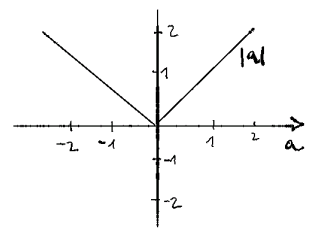
\includegraphics[width=0.4\textwidth]{betrag.png}
    \caption{Betrag verglichen mit 'clipping'. Sinus Schwingung als Input.}
    \label{fig:sinBetrag}
\end{figure}


\subsection{Potenzen, Wurzeln, Logarithmen}
\todo[inline]{Erklärender Text evtl}

\subsubsection{Potenzgesetze}

\important{ 

\emph{\textbf{Potenzgesetze}}

$$ a^n \cdot a^m = a^{n+m}$$ 

$$ \frac{a^n}{a^m} = a^{n-m}$$

$$ (a^n)^m = a^{n\cdot m}$$

$$ a^n \cdot b^n = (a \cdot b)^n$$

$$ \frac{a^n} {b^n} = \left(\frac{a} {b} \right)^n. \: b \neq 0.$$
}

\subsubsection{Wissenschaftliche Notation}
\todo[inline]{Erklärungen}
\important{

$$ x = d\cdot 10^e$$

\begin{itemize}
    \item $d$: Mantisse\footnote{ von Lateinisch 'Zugabe' oder 'Gewinn'. Siehe \cite{wiki:mantisse}}
    \item $e$: Exponent
\end{itemize}
}


\subsubsection{Logarithmen}
Konzeptuell verwandt mit der Wurzel, beantwortet er die Frage nach dem Exponenten bei gegebener Basis.

$$ 5 ^2 =25 $$

$$\sqrt[2]{25} = 5$$

$$ log_5 (25) = 2$$

\important{
    Wenn wir eine Gleichung der Art:
    $$ b^x = a $$
    Vorfinden wobei $a$ und $b$ konstanten sind und wir $x$ finden wollen und $a>0$ und $b \neq 1$ dann können wir auflösen:
    \begin{equation}
        log_b(a) = x
    \end{equation}

    Außerdem gilt allgemein:
    \begin{equation}
        log_b(b^x) = x
    \end{equation}

}



Der dekadische Logarithmus ($log_{10}$) ist u.a. praktisch, da er quasi die Frage nach den Stellen einer Zahl im dezimal System beantwortet. Ein Negatives Ergebnis gibt hier an, dass es sich um eine zahl $<1$ handelt und sein wert gibt Aufschluss auf die zahl der 'Nullen' vor dem Komma an:

\begin{itemize}
    

\item  $ log_{10}(100) = 2$
\item  $ log_{10}(1000) = 3$
\item  $ log_{10}(1) = 0$
\item  $ log_{10}(0.01) = -2$
\end{itemize}

Diese 'Eigenschaft' kann zB. benutzt werden um Visualisierungen klarer zu machen, in denen werte mit sehr Unterschiedlichen Größenordnungen Verglichen werden sollen. Siehe Abbildung \ref{fig:time_lin} im Vergleich zu \ref{fig:time_log}. Das \emph{Dezibel} fällt mehr oder weniger in diese Kategorie. 

\textbf{Der Logarithmus von 0 ist undefiniert.} Manchmal stößt man (in Computersystemen zb.) auf Ergebnisse die uns zu sagen scheinen, dass  $log(0)=-\infty$. Das ist nicht korrekt/schlampig. Natürlich scheint sich der Funktionsverlauf diesem 'Wert' anzunähern. Korrekterweise lässt sich sagen: $\lim_{x\to 0} log(x)=-\infty$. 


\subsubsection{Rechenregeln mit dem Logarithmus}
\todo[]{todo}

\important{
\begin{equation}
log_a (u \cdot v) = log_a(u) + log_a(v) \label{eq:logprods}
\end{equation}

\begin{equation}
log_a \left(\frac{u}{v}\right) = log_a(u) - log_a(v) \label{eq:logdivs}
\end{equation}

\begin{equation}
log_a (u ^ v) = v \cdot log_a(u) \label{eq:logexps}
\end{equation}

\begin{equation}
log_a \left( \frac{1}{u} \right) = - log_a(u) \label{eq:logminone}
\end{equation}
}


\begin{question}
    Leite Gleichung \ref{eq:logminone} einmal aus Gleichung \ref{eq:logdivs} und einmal aus Gleichung \ref{eq:logexps} ab! 
\end{question}

\begin{answer}
Zu \ref{eq:logdivs}: \\
Man setzt ein, und hat ein kleines Problem da die variablen Namen dafür ungünstig/verwirrend sind. Wir benennen diese also um für Gl. \ref{eq:logdivs}. Außerdem verwerfen wir die $log_a$ Notation da das $a$ hier stets irrelevant ist:
$$ log \left(\frac{x}{y}\right) = log(x) - log(y).$$ 
Wir setzen $x=1$:
$$ log \left(\frac{1}{y}\right) = log(1) - log(y).$$
Wir wissen dass $log(1) = 0$ da $\forall x \in \mathbb{R} \: , \: x^0 = 1$. 
Daher: $$ log \left(\frac{1}{y}\right) = - log(y).$$ \\

Zu \ref{eq:logexps}: \\
Wenn man im Kopf hat dass $x^{-1}=\frac{1}{x}$ ist klar, dass auch hier einsetzten hilft. Ausgehend von Gl. \ref{eq:logexps} bleiben wir bei der $x, \: y$ Notation:
$$log (x ^ y) = y \cdot log(x).$$
Da wir in Gleichung \ref{eq:logminone} dieses vorfinden: $log_a \left( \frac{1}{u} \right)$ und aber wissen dass wir umformen können zu $log_a ( u^{-1}) $ 
Wir setzten $y=-1$ und sind eigentlich schon fertig:
$$log (x ^ {-1}) = -1 \cdot log(x) = $$
$$log \left( \frac{1}{x} \right) = -log(x)$$

\end{answer} 

\subsubsection{Logarithmen 'Konvertieren'}

Gegeben $log_a(x)$ wie kann man $log_b(x)$ errechnen, also zu anderer Basis 'konvertieren'?

Man dividiert durch den $log_a(b)$:

$$ log_b(x) = \frac{log_a(x)}{log_a(b)}$$

\example{\textbf{Beispiel} \\

Gegeben den natürlichen Logarithmus einer Messung $x$ benötigt man den 2er Logarithmus. Der natürliche Logarithmus der Messgröße $x$ ist ca. $1.61$. 
$$log_2(x) = \frac{ln(x)}{ln(2)} $$
Also:
$$log_2(x) = \frac{1.61}{ln(2)} \approx 2.32$$
In diesem Beispiel war $x=5$ und wir können überprüfen dass $log_2(5) \approx 2.32$.
}
\subsubsection {Dezibel \& $dB_{FS}$}
Speziell wichtig in der (Audio-) Signalverarbeitung: $dB$ (Dezibel, ein Zehntel \emph{Bel}). 
\important{
Das $Bel$ \emph{vergleicht} 2 \emph{Leistungsgrößen}, $P_1$ und $P_2$ und erleichtert uns das Leben indem davon der Logarithmus genommen wird:
$$ L_{Bel} = log_{10} \left(\frac{P_1}{P_2}\right)$$
}

Dadurch dass wir nicht immer mit Leistungsgrößen zu tun haben, sondern manchmal zu diesen konvertieren müssen, findet sich oft der Faktor $2$ in der Formel. Konvertierung vom $Bel$ zum $Dezibel$ macht eine Multiplikation mit 10 erforderlich:

$$L = 20 \cdot log_{10}\left(\frac{x}{x_{ref}}\right)$$

Wobei im im digitalen Fall $dB_{FS}$ ('Fullscale') sich $x_{ref}$  auf den Vollausschlag $1$ bezieht und damit vereinfacht werden kann zu: 
$$L = 20 \cdot log_{10}(x)$$

\todo[]{Exkurs: Leistung eines digitalsignals via URI}
\todo[]{Andere Referenzwerte.}

\faust{Lineare Lautstärken Steuerung verglichen mit klassisch Logarithmischer.}{https://faustide.grame.fr/?autorun=1&voices=0&name=example&inline=aW1wb3J0KCJzdGRmYXVzdC5saWIiKTsKYW1wID0gaHNsaWRlcigiTGluZWFyIEFtcGxpdHVkZSIsIDAuLCAwLCAxLCAwLjAwMSk6c2kuc21vbzsKCmFtcExvZyA9IGhzbGlkZXIoIkxvZyBBbXBsaXR1ZGUiLCAtNzAuLCAtNzAsIDAsIDAuMDEpOnNpLnNtb286YmEuZGIybGluZWFyOwoKcHJvY2VzcyA9IG5vLnBpbmtfbm9pc2UgKiBhbXAgKyBuby5waW5rX25vaXNlICogYW1wTG9nPDpfLF87}

\todo[]{Wurzeln}



\begin{figure}[h!]
    \centering
    %% Creator: Matplotlib, PGF backend
%%
%% To include the figure in your LaTeX document, write
%%   \input{<filename>.pgf}
%%
%% Make sure the required packages are loaded in your preamble
%%   \usepackage{pgf}
%%
%% Also ensure that all the required font packages are loaded; for instance,
%% the lmodern package is sometimes necessary when using math font.
%%   \usepackage{lmodern}
%%
%% Figures using additional raster images can only be included by \input if
%% they are in the same directory as the main LaTeX file. For loading figures
%% from other directories you can use the `import` package
%%   \usepackage{import}
%%
%% and then include the figures with
%%   \import{<path to file>}{<filename>.pgf}
%%
%% Matplotlib used the following preamble
%%   \def\mathdefault#1{#1}
%%   \everymath=\expandafter{\the\everymath\displaystyle}
%%   \usepackage{amsmath}
%%   \makeatletter\@ifpackageloaded{underscore}{}{\usepackage[strings]{underscore}}\makeatother
%%
\begingroup%
\makeatletter%
\begin{pgfpicture}%
\pgfpathrectangle{\pgfpointorigin}{\pgfqpoint{5.504137in}{4.320382in}}%
\pgfusepath{use as bounding box, clip}%
\begin{pgfscope}%
\pgfsetbuttcap%
\pgfsetmiterjoin%
\definecolor{currentfill}{rgb}{1.000000,1.000000,1.000000}%
\pgfsetfillcolor{currentfill}%
\pgfsetlinewidth{0.000000pt}%
\definecolor{currentstroke}{rgb}{1.000000,1.000000,1.000000}%
\pgfsetstrokecolor{currentstroke}%
\pgfsetdash{}{0pt}%
\pgfpathmoveto{\pgfqpoint{0.000000in}{0.000000in}}%
\pgfpathlineto{\pgfqpoint{5.504137in}{0.000000in}}%
\pgfpathlineto{\pgfqpoint{5.504137in}{4.320382in}}%
\pgfpathlineto{\pgfqpoint{0.000000in}{4.320382in}}%
\pgfpathlineto{\pgfqpoint{0.000000in}{0.000000in}}%
\pgfpathclose%
\pgfusepath{fill}%
\end{pgfscope}%
\begin{pgfscope}%
\pgfsetbuttcap%
\pgfsetmiterjoin%
\definecolor{currentfill}{rgb}{1.000000,1.000000,1.000000}%
\pgfsetfillcolor{currentfill}%
\pgfsetlinewidth{0.000000pt}%
\definecolor{currentstroke}{rgb}{0.000000,0.000000,0.000000}%
\pgfsetstrokecolor{currentstroke}%
\pgfsetstrokeopacity{0.000000}%
\pgfsetdash{}{0pt}%
\pgfpathmoveto{\pgfqpoint{0.444137in}{0.524382in}}%
\pgfpathlineto{\pgfqpoint{5.404137in}{0.524382in}}%
\pgfpathlineto{\pgfqpoint{5.404137in}{4.220382in}}%
\pgfpathlineto{\pgfqpoint{0.444137in}{4.220382in}}%
\pgfpathlineto{\pgfqpoint{0.444137in}{0.524382in}}%
\pgfpathclose%
\pgfusepath{fill}%
\end{pgfscope}%
\begin{pgfscope}%
\pgfpathrectangle{\pgfqpoint{0.444137in}{0.524382in}}{\pgfqpoint{4.960000in}{3.696000in}}%
\pgfusepath{clip}%
\pgfsetrectcap%
\pgfsetroundjoin%
\pgfsetlinewidth{0.803000pt}%
\definecolor{currentstroke}{rgb}{0.690196,0.690196,0.690196}%
\pgfsetstrokecolor{currentstroke}%
\pgfsetdash{}{0pt}%
\pgfpathmoveto{\pgfqpoint{0.667787in}{0.524382in}}%
\pgfpathlineto{\pgfqpoint{0.667787in}{4.220382in}}%
\pgfusepath{stroke}%
\end{pgfscope}%
\begin{pgfscope}%
\pgfsetbuttcap%
\pgfsetroundjoin%
\definecolor{currentfill}{rgb}{0.000000,0.000000,0.000000}%
\pgfsetfillcolor{currentfill}%
\pgfsetlinewidth{0.803000pt}%
\definecolor{currentstroke}{rgb}{0.000000,0.000000,0.000000}%
\pgfsetstrokecolor{currentstroke}%
\pgfsetdash{}{0pt}%
\pgfsys@defobject{currentmarker}{\pgfqpoint{0.000000in}{-0.048611in}}{\pgfqpoint{0.000000in}{0.000000in}}{%
\pgfpathmoveto{\pgfqpoint{0.000000in}{0.000000in}}%
\pgfpathlineto{\pgfqpoint{0.000000in}{-0.048611in}}%
\pgfusepath{stroke,fill}%
}%
\begin{pgfscope}%
\pgfsys@transformshift{0.667787in}{0.524382in}%
\pgfsys@useobject{currentmarker}{}%
\end{pgfscope}%
\end{pgfscope}%
\begin{pgfscope}%
\definecolor{textcolor}{rgb}{0.000000,0.000000,0.000000}%
\pgfsetstrokecolor{textcolor}%
\pgfsetfillcolor{textcolor}%
\pgftext[x=0.667787in,y=0.427160in,,top]{\color{textcolor}{\rmfamily\fontsize{10.000000}{12.000000}\selectfont\catcode`\^=\active\def^{\ifmmode\sp\else\^{}\fi}\catcode`\%=\active\def%{\%}0.0}}%
\end{pgfscope}%
\begin{pgfscope}%
\pgfpathrectangle{\pgfqpoint{0.444137in}{0.524382in}}{\pgfqpoint{4.960000in}{3.696000in}}%
\pgfusepath{clip}%
\pgfsetrectcap%
\pgfsetroundjoin%
\pgfsetlinewidth{0.803000pt}%
\definecolor{currentstroke}{rgb}{0.690196,0.690196,0.690196}%
\pgfsetstrokecolor{currentstroke}%
\pgfsetdash{}{0pt}%
\pgfpathmoveto{\pgfqpoint{1.569966in}{0.524382in}}%
\pgfpathlineto{\pgfqpoint{1.569966in}{4.220382in}}%
\pgfusepath{stroke}%
\end{pgfscope}%
\begin{pgfscope}%
\pgfsetbuttcap%
\pgfsetroundjoin%
\definecolor{currentfill}{rgb}{0.000000,0.000000,0.000000}%
\pgfsetfillcolor{currentfill}%
\pgfsetlinewidth{0.803000pt}%
\definecolor{currentstroke}{rgb}{0.000000,0.000000,0.000000}%
\pgfsetstrokecolor{currentstroke}%
\pgfsetdash{}{0pt}%
\pgfsys@defobject{currentmarker}{\pgfqpoint{0.000000in}{-0.048611in}}{\pgfqpoint{0.000000in}{0.000000in}}{%
\pgfpathmoveto{\pgfqpoint{0.000000in}{0.000000in}}%
\pgfpathlineto{\pgfqpoint{0.000000in}{-0.048611in}}%
\pgfusepath{stroke,fill}%
}%
\begin{pgfscope}%
\pgfsys@transformshift{1.569966in}{0.524382in}%
\pgfsys@useobject{currentmarker}{}%
\end{pgfscope}%
\end{pgfscope}%
\begin{pgfscope}%
\definecolor{textcolor}{rgb}{0.000000,0.000000,0.000000}%
\pgfsetstrokecolor{textcolor}%
\pgfsetfillcolor{textcolor}%
\pgftext[x=1.569966in,y=0.427160in,,top]{\color{textcolor}{\rmfamily\fontsize{10.000000}{12.000000}\selectfont\catcode`\^=\active\def^{\ifmmode\sp\else\^{}\fi}\catcode`\%=\active\def%{\%}0.5}}%
\end{pgfscope}%
\begin{pgfscope}%
\pgfpathrectangle{\pgfqpoint{0.444137in}{0.524382in}}{\pgfqpoint{4.960000in}{3.696000in}}%
\pgfusepath{clip}%
\pgfsetrectcap%
\pgfsetroundjoin%
\pgfsetlinewidth{0.803000pt}%
\definecolor{currentstroke}{rgb}{0.690196,0.690196,0.690196}%
\pgfsetstrokecolor{currentstroke}%
\pgfsetdash{}{0pt}%
\pgfpathmoveto{\pgfqpoint{2.472145in}{0.524382in}}%
\pgfpathlineto{\pgfqpoint{2.472145in}{4.220382in}}%
\pgfusepath{stroke}%
\end{pgfscope}%
\begin{pgfscope}%
\pgfsetbuttcap%
\pgfsetroundjoin%
\definecolor{currentfill}{rgb}{0.000000,0.000000,0.000000}%
\pgfsetfillcolor{currentfill}%
\pgfsetlinewidth{0.803000pt}%
\definecolor{currentstroke}{rgb}{0.000000,0.000000,0.000000}%
\pgfsetstrokecolor{currentstroke}%
\pgfsetdash{}{0pt}%
\pgfsys@defobject{currentmarker}{\pgfqpoint{0.000000in}{-0.048611in}}{\pgfqpoint{0.000000in}{0.000000in}}{%
\pgfpathmoveto{\pgfqpoint{0.000000in}{0.000000in}}%
\pgfpathlineto{\pgfqpoint{0.000000in}{-0.048611in}}%
\pgfusepath{stroke,fill}%
}%
\begin{pgfscope}%
\pgfsys@transformshift{2.472145in}{0.524382in}%
\pgfsys@useobject{currentmarker}{}%
\end{pgfscope}%
\end{pgfscope}%
\begin{pgfscope}%
\definecolor{textcolor}{rgb}{0.000000,0.000000,0.000000}%
\pgfsetstrokecolor{textcolor}%
\pgfsetfillcolor{textcolor}%
\pgftext[x=2.472145in,y=0.427160in,,top]{\color{textcolor}{\rmfamily\fontsize{10.000000}{12.000000}\selectfont\catcode`\^=\active\def^{\ifmmode\sp\else\^{}\fi}\catcode`\%=\active\def%{\%}1.0}}%
\end{pgfscope}%
\begin{pgfscope}%
\pgfpathrectangle{\pgfqpoint{0.444137in}{0.524382in}}{\pgfqpoint{4.960000in}{3.696000in}}%
\pgfusepath{clip}%
\pgfsetrectcap%
\pgfsetroundjoin%
\pgfsetlinewidth{0.803000pt}%
\definecolor{currentstroke}{rgb}{0.690196,0.690196,0.690196}%
\pgfsetstrokecolor{currentstroke}%
\pgfsetdash{}{0pt}%
\pgfpathmoveto{\pgfqpoint{3.374324in}{0.524382in}}%
\pgfpathlineto{\pgfqpoint{3.374324in}{4.220382in}}%
\pgfusepath{stroke}%
\end{pgfscope}%
\begin{pgfscope}%
\pgfsetbuttcap%
\pgfsetroundjoin%
\definecolor{currentfill}{rgb}{0.000000,0.000000,0.000000}%
\pgfsetfillcolor{currentfill}%
\pgfsetlinewidth{0.803000pt}%
\definecolor{currentstroke}{rgb}{0.000000,0.000000,0.000000}%
\pgfsetstrokecolor{currentstroke}%
\pgfsetdash{}{0pt}%
\pgfsys@defobject{currentmarker}{\pgfqpoint{0.000000in}{-0.048611in}}{\pgfqpoint{0.000000in}{0.000000in}}{%
\pgfpathmoveto{\pgfqpoint{0.000000in}{0.000000in}}%
\pgfpathlineto{\pgfqpoint{0.000000in}{-0.048611in}}%
\pgfusepath{stroke,fill}%
}%
\begin{pgfscope}%
\pgfsys@transformshift{3.374324in}{0.524382in}%
\pgfsys@useobject{currentmarker}{}%
\end{pgfscope}%
\end{pgfscope}%
\begin{pgfscope}%
\definecolor{textcolor}{rgb}{0.000000,0.000000,0.000000}%
\pgfsetstrokecolor{textcolor}%
\pgfsetfillcolor{textcolor}%
\pgftext[x=3.374324in,y=0.427160in,,top]{\color{textcolor}{\rmfamily\fontsize{10.000000}{12.000000}\selectfont\catcode`\^=\active\def^{\ifmmode\sp\else\^{}\fi}\catcode`\%=\active\def%{\%}1.5}}%
\end{pgfscope}%
\begin{pgfscope}%
\pgfpathrectangle{\pgfqpoint{0.444137in}{0.524382in}}{\pgfqpoint{4.960000in}{3.696000in}}%
\pgfusepath{clip}%
\pgfsetrectcap%
\pgfsetroundjoin%
\pgfsetlinewidth{0.803000pt}%
\definecolor{currentstroke}{rgb}{0.690196,0.690196,0.690196}%
\pgfsetstrokecolor{currentstroke}%
\pgfsetdash{}{0pt}%
\pgfpathmoveto{\pgfqpoint{4.276503in}{0.524382in}}%
\pgfpathlineto{\pgfqpoint{4.276503in}{4.220382in}}%
\pgfusepath{stroke}%
\end{pgfscope}%
\begin{pgfscope}%
\pgfsetbuttcap%
\pgfsetroundjoin%
\definecolor{currentfill}{rgb}{0.000000,0.000000,0.000000}%
\pgfsetfillcolor{currentfill}%
\pgfsetlinewidth{0.803000pt}%
\definecolor{currentstroke}{rgb}{0.000000,0.000000,0.000000}%
\pgfsetstrokecolor{currentstroke}%
\pgfsetdash{}{0pt}%
\pgfsys@defobject{currentmarker}{\pgfqpoint{0.000000in}{-0.048611in}}{\pgfqpoint{0.000000in}{0.000000in}}{%
\pgfpathmoveto{\pgfqpoint{0.000000in}{0.000000in}}%
\pgfpathlineto{\pgfqpoint{0.000000in}{-0.048611in}}%
\pgfusepath{stroke,fill}%
}%
\begin{pgfscope}%
\pgfsys@transformshift{4.276503in}{0.524382in}%
\pgfsys@useobject{currentmarker}{}%
\end{pgfscope}%
\end{pgfscope}%
\begin{pgfscope}%
\definecolor{textcolor}{rgb}{0.000000,0.000000,0.000000}%
\pgfsetstrokecolor{textcolor}%
\pgfsetfillcolor{textcolor}%
\pgftext[x=4.276503in,y=0.427160in,,top]{\color{textcolor}{\rmfamily\fontsize{10.000000}{12.000000}\selectfont\catcode`\^=\active\def^{\ifmmode\sp\else\^{}\fi}\catcode`\%=\active\def%{\%}2.0}}%
\end{pgfscope}%
\begin{pgfscope}%
\pgfpathrectangle{\pgfqpoint{0.444137in}{0.524382in}}{\pgfqpoint{4.960000in}{3.696000in}}%
\pgfusepath{clip}%
\pgfsetrectcap%
\pgfsetroundjoin%
\pgfsetlinewidth{0.803000pt}%
\definecolor{currentstroke}{rgb}{0.690196,0.690196,0.690196}%
\pgfsetstrokecolor{currentstroke}%
\pgfsetdash{}{0pt}%
\pgfpathmoveto{\pgfqpoint{5.178682in}{0.524382in}}%
\pgfpathlineto{\pgfqpoint{5.178682in}{4.220382in}}%
\pgfusepath{stroke}%
\end{pgfscope}%
\begin{pgfscope}%
\pgfsetbuttcap%
\pgfsetroundjoin%
\definecolor{currentfill}{rgb}{0.000000,0.000000,0.000000}%
\pgfsetfillcolor{currentfill}%
\pgfsetlinewidth{0.803000pt}%
\definecolor{currentstroke}{rgb}{0.000000,0.000000,0.000000}%
\pgfsetstrokecolor{currentstroke}%
\pgfsetdash{}{0pt}%
\pgfsys@defobject{currentmarker}{\pgfqpoint{0.000000in}{-0.048611in}}{\pgfqpoint{0.000000in}{0.000000in}}{%
\pgfpathmoveto{\pgfqpoint{0.000000in}{0.000000in}}%
\pgfpathlineto{\pgfqpoint{0.000000in}{-0.048611in}}%
\pgfusepath{stroke,fill}%
}%
\begin{pgfscope}%
\pgfsys@transformshift{5.178682in}{0.524382in}%
\pgfsys@useobject{currentmarker}{}%
\end{pgfscope}%
\end{pgfscope}%
\begin{pgfscope}%
\definecolor{textcolor}{rgb}{0.000000,0.000000,0.000000}%
\pgfsetstrokecolor{textcolor}%
\pgfsetfillcolor{textcolor}%
\pgftext[x=5.178682in,y=0.427160in,,top]{\color{textcolor}{\rmfamily\fontsize{10.000000}{12.000000}\selectfont\catcode`\^=\active\def^{\ifmmode\sp\else\^{}\fi}\catcode`\%=\active\def%{\%}2.5}}%
\end{pgfscope}%
\begin{pgfscope}%
\definecolor{textcolor}{rgb}{0.000000,0.000000,0.000000}%
\pgfsetstrokecolor{textcolor}%
\pgfsetfillcolor{textcolor}%
\pgftext[x=2.924137in,y=0.248148in,,top]{\color{textcolor}{\rmfamily\fontsize{12.000000}{14.400000}\selectfont\catcode`\^=\active\def^{\ifmmode\sp\else\^{}\fi}\catcode`\%=\active\def%{\%}$x$}}%
\end{pgfscope}%
\begin{pgfscope}%
\pgfpathrectangle{\pgfqpoint{0.444137in}{0.524382in}}{\pgfqpoint{4.960000in}{3.696000in}}%
\pgfusepath{clip}%
\pgfsetrectcap%
\pgfsetroundjoin%
\pgfsetlinewidth{0.803000pt}%
\definecolor{currentstroke}{rgb}{0.690196,0.690196,0.690196}%
\pgfsetstrokecolor{currentstroke}%
\pgfsetdash{}{0pt}%
\pgfpathmoveto{\pgfqpoint{0.444137in}{0.692382in}}%
\pgfpathlineto{\pgfqpoint{5.404137in}{0.692382in}}%
\pgfusepath{stroke}%
\end{pgfscope}%
\begin{pgfscope}%
\pgfsetbuttcap%
\pgfsetroundjoin%
\definecolor{currentfill}{rgb}{0.000000,0.000000,0.000000}%
\pgfsetfillcolor{currentfill}%
\pgfsetlinewidth{0.803000pt}%
\definecolor{currentstroke}{rgb}{0.000000,0.000000,0.000000}%
\pgfsetstrokecolor{currentstroke}%
\pgfsetdash{}{0pt}%
\pgfsys@defobject{currentmarker}{\pgfqpoint{-0.048611in}{0.000000in}}{\pgfqpoint{-0.000000in}{0.000000in}}{%
\pgfpathmoveto{\pgfqpoint{-0.000000in}{0.000000in}}%
\pgfpathlineto{\pgfqpoint{-0.048611in}{0.000000in}}%
\pgfusepath{stroke,fill}%
}%
\begin{pgfscope}%
\pgfsys@transformshift{0.444137in}{0.692382in}%
\pgfsys@useobject{currentmarker}{}%
\end{pgfscope}%
\end{pgfscope}%
\begin{pgfscope}%
\definecolor{textcolor}{rgb}{0.000000,0.000000,0.000000}%
\pgfsetstrokecolor{textcolor}%
\pgfsetfillcolor{textcolor}%
\pgftext[x=0.100000in, y=0.644157in, left, base]{\color{textcolor}{\rmfamily\fontsize{10.000000}{12.000000}\selectfont\catcode`\^=\active\def^{\ifmmode\sp\else\^{}\fi}\catcode`\%=\active\def%{\%}\ensuremath{-}60}}%
\end{pgfscope}%
\begin{pgfscope}%
\pgfpathrectangle{\pgfqpoint{0.444137in}{0.524382in}}{\pgfqpoint{4.960000in}{3.696000in}}%
\pgfusepath{clip}%
\pgfsetrectcap%
\pgfsetroundjoin%
\pgfsetlinewidth{0.803000pt}%
\definecolor{currentstroke}{rgb}{0.690196,0.690196,0.690196}%
\pgfsetstrokecolor{currentstroke}%
\pgfsetdash{}{0pt}%
\pgfpathmoveto{\pgfqpoint{0.444137in}{1.186799in}}%
\pgfpathlineto{\pgfqpoint{5.404137in}{1.186799in}}%
\pgfusepath{stroke}%
\end{pgfscope}%
\begin{pgfscope}%
\pgfsetbuttcap%
\pgfsetroundjoin%
\definecolor{currentfill}{rgb}{0.000000,0.000000,0.000000}%
\pgfsetfillcolor{currentfill}%
\pgfsetlinewidth{0.803000pt}%
\definecolor{currentstroke}{rgb}{0.000000,0.000000,0.000000}%
\pgfsetstrokecolor{currentstroke}%
\pgfsetdash{}{0pt}%
\pgfsys@defobject{currentmarker}{\pgfqpoint{-0.048611in}{0.000000in}}{\pgfqpoint{-0.000000in}{0.000000in}}{%
\pgfpathmoveto{\pgfqpoint{-0.000000in}{0.000000in}}%
\pgfpathlineto{\pgfqpoint{-0.048611in}{0.000000in}}%
\pgfusepath{stroke,fill}%
}%
\begin{pgfscope}%
\pgfsys@transformshift{0.444137in}{1.186799in}%
\pgfsys@useobject{currentmarker}{}%
\end{pgfscope}%
\end{pgfscope}%
\begin{pgfscope}%
\definecolor{textcolor}{rgb}{0.000000,0.000000,0.000000}%
\pgfsetstrokecolor{textcolor}%
\pgfsetfillcolor{textcolor}%
\pgftext[x=0.100000in, y=1.138574in, left, base]{\color{textcolor}{\rmfamily\fontsize{10.000000}{12.000000}\selectfont\catcode`\^=\active\def^{\ifmmode\sp\else\^{}\fi}\catcode`\%=\active\def%{\%}\ensuremath{-}50}}%
\end{pgfscope}%
\begin{pgfscope}%
\pgfpathrectangle{\pgfqpoint{0.444137in}{0.524382in}}{\pgfqpoint{4.960000in}{3.696000in}}%
\pgfusepath{clip}%
\pgfsetrectcap%
\pgfsetroundjoin%
\pgfsetlinewidth{0.803000pt}%
\definecolor{currentstroke}{rgb}{0.690196,0.690196,0.690196}%
\pgfsetstrokecolor{currentstroke}%
\pgfsetdash{}{0pt}%
\pgfpathmoveto{\pgfqpoint{0.444137in}{1.681216in}}%
\pgfpathlineto{\pgfqpoint{5.404137in}{1.681216in}}%
\pgfusepath{stroke}%
\end{pgfscope}%
\begin{pgfscope}%
\pgfsetbuttcap%
\pgfsetroundjoin%
\definecolor{currentfill}{rgb}{0.000000,0.000000,0.000000}%
\pgfsetfillcolor{currentfill}%
\pgfsetlinewidth{0.803000pt}%
\definecolor{currentstroke}{rgb}{0.000000,0.000000,0.000000}%
\pgfsetstrokecolor{currentstroke}%
\pgfsetdash{}{0pt}%
\pgfsys@defobject{currentmarker}{\pgfqpoint{-0.048611in}{0.000000in}}{\pgfqpoint{-0.000000in}{0.000000in}}{%
\pgfpathmoveto{\pgfqpoint{-0.000000in}{0.000000in}}%
\pgfpathlineto{\pgfqpoint{-0.048611in}{0.000000in}}%
\pgfusepath{stroke,fill}%
}%
\begin{pgfscope}%
\pgfsys@transformshift{0.444137in}{1.681216in}%
\pgfsys@useobject{currentmarker}{}%
\end{pgfscope}%
\end{pgfscope}%
\begin{pgfscope}%
\definecolor{textcolor}{rgb}{0.000000,0.000000,0.000000}%
\pgfsetstrokecolor{textcolor}%
\pgfsetfillcolor{textcolor}%
\pgftext[x=0.100000in, y=1.632991in, left, base]{\color{textcolor}{\rmfamily\fontsize{10.000000}{12.000000}\selectfont\catcode`\^=\active\def^{\ifmmode\sp\else\^{}\fi}\catcode`\%=\active\def%{\%}\ensuremath{-}40}}%
\end{pgfscope}%
\begin{pgfscope}%
\pgfpathrectangle{\pgfqpoint{0.444137in}{0.524382in}}{\pgfqpoint{4.960000in}{3.696000in}}%
\pgfusepath{clip}%
\pgfsetrectcap%
\pgfsetroundjoin%
\pgfsetlinewidth{0.803000pt}%
\definecolor{currentstroke}{rgb}{0.690196,0.690196,0.690196}%
\pgfsetstrokecolor{currentstroke}%
\pgfsetdash{}{0pt}%
\pgfpathmoveto{\pgfqpoint{0.444137in}{2.175634in}}%
\pgfpathlineto{\pgfqpoint{5.404137in}{2.175634in}}%
\pgfusepath{stroke}%
\end{pgfscope}%
\begin{pgfscope}%
\pgfsetbuttcap%
\pgfsetroundjoin%
\definecolor{currentfill}{rgb}{0.000000,0.000000,0.000000}%
\pgfsetfillcolor{currentfill}%
\pgfsetlinewidth{0.803000pt}%
\definecolor{currentstroke}{rgb}{0.000000,0.000000,0.000000}%
\pgfsetstrokecolor{currentstroke}%
\pgfsetdash{}{0pt}%
\pgfsys@defobject{currentmarker}{\pgfqpoint{-0.048611in}{0.000000in}}{\pgfqpoint{-0.000000in}{0.000000in}}{%
\pgfpathmoveto{\pgfqpoint{-0.000000in}{0.000000in}}%
\pgfpathlineto{\pgfqpoint{-0.048611in}{0.000000in}}%
\pgfusepath{stroke,fill}%
}%
\begin{pgfscope}%
\pgfsys@transformshift{0.444137in}{2.175634in}%
\pgfsys@useobject{currentmarker}{}%
\end{pgfscope}%
\end{pgfscope}%
\begin{pgfscope}%
\definecolor{textcolor}{rgb}{0.000000,0.000000,0.000000}%
\pgfsetstrokecolor{textcolor}%
\pgfsetfillcolor{textcolor}%
\pgftext[x=0.100000in, y=2.127408in, left, base]{\color{textcolor}{\rmfamily\fontsize{10.000000}{12.000000}\selectfont\catcode`\^=\active\def^{\ifmmode\sp\else\^{}\fi}\catcode`\%=\active\def%{\%}\ensuremath{-}30}}%
\end{pgfscope}%
\begin{pgfscope}%
\pgfpathrectangle{\pgfqpoint{0.444137in}{0.524382in}}{\pgfqpoint{4.960000in}{3.696000in}}%
\pgfusepath{clip}%
\pgfsetrectcap%
\pgfsetroundjoin%
\pgfsetlinewidth{0.803000pt}%
\definecolor{currentstroke}{rgb}{0.690196,0.690196,0.690196}%
\pgfsetstrokecolor{currentstroke}%
\pgfsetdash{}{0pt}%
\pgfpathmoveto{\pgfqpoint{0.444137in}{2.670051in}}%
\pgfpathlineto{\pgfqpoint{5.404137in}{2.670051in}}%
\pgfusepath{stroke}%
\end{pgfscope}%
\begin{pgfscope}%
\pgfsetbuttcap%
\pgfsetroundjoin%
\definecolor{currentfill}{rgb}{0.000000,0.000000,0.000000}%
\pgfsetfillcolor{currentfill}%
\pgfsetlinewidth{0.803000pt}%
\definecolor{currentstroke}{rgb}{0.000000,0.000000,0.000000}%
\pgfsetstrokecolor{currentstroke}%
\pgfsetdash{}{0pt}%
\pgfsys@defobject{currentmarker}{\pgfqpoint{-0.048611in}{0.000000in}}{\pgfqpoint{-0.000000in}{0.000000in}}{%
\pgfpathmoveto{\pgfqpoint{-0.000000in}{0.000000in}}%
\pgfpathlineto{\pgfqpoint{-0.048611in}{0.000000in}}%
\pgfusepath{stroke,fill}%
}%
\begin{pgfscope}%
\pgfsys@transformshift{0.444137in}{2.670051in}%
\pgfsys@useobject{currentmarker}{}%
\end{pgfscope}%
\end{pgfscope}%
\begin{pgfscope}%
\definecolor{textcolor}{rgb}{0.000000,0.000000,0.000000}%
\pgfsetstrokecolor{textcolor}%
\pgfsetfillcolor{textcolor}%
\pgftext[x=0.100000in, y=2.621825in, left, base]{\color{textcolor}{\rmfamily\fontsize{10.000000}{12.000000}\selectfont\catcode`\^=\active\def^{\ifmmode\sp\else\^{}\fi}\catcode`\%=\active\def%{\%}\ensuremath{-}20}}%
\end{pgfscope}%
\begin{pgfscope}%
\pgfpathrectangle{\pgfqpoint{0.444137in}{0.524382in}}{\pgfqpoint{4.960000in}{3.696000in}}%
\pgfusepath{clip}%
\pgfsetrectcap%
\pgfsetroundjoin%
\pgfsetlinewidth{0.803000pt}%
\definecolor{currentstroke}{rgb}{0.690196,0.690196,0.690196}%
\pgfsetstrokecolor{currentstroke}%
\pgfsetdash{}{0pt}%
\pgfpathmoveto{\pgfqpoint{0.444137in}{3.164468in}}%
\pgfpathlineto{\pgfqpoint{5.404137in}{3.164468in}}%
\pgfusepath{stroke}%
\end{pgfscope}%
\begin{pgfscope}%
\pgfsetbuttcap%
\pgfsetroundjoin%
\definecolor{currentfill}{rgb}{0.000000,0.000000,0.000000}%
\pgfsetfillcolor{currentfill}%
\pgfsetlinewidth{0.803000pt}%
\definecolor{currentstroke}{rgb}{0.000000,0.000000,0.000000}%
\pgfsetstrokecolor{currentstroke}%
\pgfsetdash{}{0pt}%
\pgfsys@defobject{currentmarker}{\pgfqpoint{-0.048611in}{0.000000in}}{\pgfqpoint{-0.000000in}{0.000000in}}{%
\pgfpathmoveto{\pgfqpoint{-0.000000in}{0.000000in}}%
\pgfpathlineto{\pgfqpoint{-0.048611in}{0.000000in}}%
\pgfusepath{stroke,fill}%
}%
\begin{pgfscope}%
\pgfsys@transformshift{0.444137in}{3.164468in}%
\pgfsys@useobject{currentmarker}{}%
\end{pgfscope}%
\end{pgfscope}%
\begin{pgfscope}%
\definecolor{textcolor}{rgb}{0.000000,0.000000,0.000000}%
\pgfsetstrokecolor{textcolor}%
\pgfsetfillcolor{textcolor}%
\pgftext[x=0.100000in, y=3.116243in, left, base]{\color{textcolor}{\rmfamily\fontsize{10.000000}{12.000000}\selectfont\catcode`\^=\active\def^{\ifmmode\sp\else\^{}\fi}\catcode`\%=\active\def%{\%}\ensuremath{-}10}}%
\end{pgfscope}%
\begin{pgfscope}%
\pgfpathrectangle{\pgfqpoint{0.444137in}{0.524382in}}{\pgfqpoint{4.960000in}{3.696000in}}%
\pgfusepath{clip}%
\pgfsetrectcap%
\pgfsetroundjoin%
\pgfsetlinewidth{0.803000pt}%
\definecolor{currentstroke}{rgb}{0.690196,0.690196,0.690196}%
\pgfsetstrokecolor{currentstroke}%
\pgfsetdash{}{0pt}%
\pgfpathmoveto{\pgfqpoint{0.444137in}{3.658885in}}%
\pgfpathlineto{\pgfqpoint{5.404137in}{3.658885in}}%
\pgfusepath{stroke}%
\end{pgfscope}%
\begin{pgfscope}%
\pgfsetbuttcap%
\pgfsetroundjoin%
\definecolor{currentfill}{rgb}{0.000000,0.000000,0.000000}%
\pgfsetfillcolor{currentfill}%
\pgfsetlinewidth{0.803000pt}%
\definecolor{currentstroke}{rgb}{0.000000,0.000000,0.000000}%
\pgfsetstrokecolor{currentstroke}%
\pgfsetdash{}{0pt}%
\pgfsys@defobject{currentmarker}{\pgfqpoint{-0.048611in}{0.000000in}}{\pgfqpoint{-0.000000in}{0.000000in}}{%
\pgfpathmoveto{\pgfqpoint{-0.000000in}{0.000000in}}%
\pgfpathlineto{\pgfqpoint{-0.048611in}{0.000000in}}%
\pgfusepath{stroke,fill}%
}%
\begin{pgfscope}%
\pgfsys@transformshift{0.444137in}{3.658885in}%
\pgfsys@useobject{currentmarker}{}%
\end{pgfscope}%
\end{pgfscope}%
\begin{pgfscope}%
\definecolor{textcolor}{rgb}{0.000000,0.000000,0.000000}%
\pgfsetstrokecolor{textcolor}%
\pgfsetfillcolor{textcolor}%
\pgftext[x=0.277470in, y=3.610660in, left, base]{\color{textcolor}{\rmfamily\fontsize{10.000000}{12.000000}\selectfont\catcode`\^=\active\def^{\ifmmode\sp\else\^{}\fi}\catcode`\%=\active\def%{\%}0}}%
\end{pgfscope}%
\begin{pgfscope}%
\pgfpathrectangle{\pgfqpoint{0.444137in}{0.524382in}}{\pgfqpoint{4.960000in}{3.696000in}}%
\pgfusepath{clip}%
\pgfsetrectcap%
\pgfsetroundjoin%
\pgfsetlinewidth{0.803000pt}%
\definecolor{currentstroke}{rgb}{0.690196,0.690196,0.690196}%
\pgfsetstrokecolor{currentstroke}%
\pgfsetdash{}{0pt}%
\pgfpathmoveto{\pgfqpoint{0.444137in}{4.153302in}}%
\pgfpathlineto{\pgfqpoint{5.404137in}{4.153302in}}%
\pgfusepath{stroke}%
\end{pgfscope}%
\begin{pgfscope}%
\pgfsetbuttcap%
\pgfsetroundjoin%
\definecolor{currentfill}{rgb}{0.000000,0.000000,0.000000}%
\pgfsetfillcolor{currentfill}%
\pgfsetlinewidth{0.803000pt}%
\definecolor{currentstroke}{rgb}{0.000000,0.000000,0.000000}%
\pgfsetstrokecolor{currentstroke}%
\pgfsetdash{}{0pt}%
\pgfsys@defobject{currentmarker}{\pgfqpoint{-0.048611in}{0.000000in}}{\pgfqpoint{-0.000000in}{0.000000in}}{%
\pgfpathmoveto{\pgfqpoint{-0.000000in}{0.000000in}}%
\pgfpathlineto{\pgfqpoint{-0.048611in}{0.000000in}}%
\pgfusepath{stroke,fill}%
}%
\begin{pgfscope}%
\pgfsys@transformshift{0.444137in}{4.153302in}%
\pgfsys@useobject{currentmarker}{}%
\end{pgfscope}%
\end{pgfscope}%
\begin{pgfscope}%
\definecolor{textcolor}{rgb}{0.000000,0.000000,0.000000}%
\pgfsetstrokecolor{textcolor}%
\pgfsetfillcolor{textcolor}%
\pgftext[x=0.208025in, y=4.105077in, left, base]{\color{textcolor}{\rmfamily\fontsize{10.000000}{12.000000}\selectfont\catcode`\^=\active\def^{\ifmmode\sp\else\^{}\fi}\catcode`\%=\active\def%{\%}10}}%
\end{pgfscope}%
\begin{pgfscope}%
\pgfpathrectangle{\pgfqpoint{0.444137in}{0.524382in}}{\pgfqpoint{4.960000in}{3.696000in}}%
\pgfusepath{clip}%
\pgfsetrectcap%
\pgfsetroundjoin%
\pgfsetlinewidth{1.505625pt}%
\definecolor{currentstroke}{rgb}{0.000000,0.000000,0.000000}%
\pgfsetstrokecolor{currentstroke}%
\pgfsetdash{}{0pt}%
\pgfpathmoveto{\pgfqpoint{0.669591in}{0.692382in}}%
\pgfpathlineto{\pgfqpoint{0.674105in}{1.230559in}}%
\pgfpathlineto{\pgfqpoint{0.678618in}{1.462060in}}%
\pgfpathlineto{\pgfqpoint{0.683132in}{1.611651in}}%
\pgfpathlineto{\pgfqpoint{0.692159in}{1.810334in}}%
\pgfpathlineto{\pgfqpoint{0.701186in}{1.945649in}}%
\pgfpathlineto{\pgfqpoint{0.710214in}{2.048388in}}%
\pgfpathlineto{\pgfqpoint{0.719241in}{2.131231in}}%
\pgfpathlineto{\pgfqpoint{0.732782in}{2.231558in}}%
\pgfpathlineto{\pgfqpoint{0.746322in}{2.312828in}}%
\pgfpathlineto{\pgfqpoint{0.759863in}{2.381139in}}%
\pgfpathlineto{\pgfqpoint{0.773404in}{2.440060in}}%
\pgfpathlineto{\pgfqpoint{0.791458in}{2.507830in}}%
\pgfpathlineto{\pgfqpoint{0.809513in}{2.566349in}}%
\pgfpathlineto{\pgfqpoint{0.827567in}{2.617841in}}%
\pgfpathlineto{\pgfqpoint{0.850135in}{2.674579in}}%
\pgfpathlineto{\pgfqpoint{0.872703in}{2.724688in}}%
\pgfpathlineto{\pgfqpoint{0.895271in}{2.769556in}}%
\pgfpathlineto{\pgfqpoint{0.922353in}{2.817860in}}%
\pgfpathlineto{\pgfqpoint{0.949435in}{2.861275in}}%
\pgfpathlineto{\pgfqpoint{0.976516in}{2.900702in}}%
\pgfpathlineto{\pgfqpoint{1.008111in}{2.942545in}}%
\pgfpathlineto{\pgfqpoint{1.039707in}{2.980670in}}%
\pgfpathlineto{\pgfqpoint{1.075815in}{3.020462in}}%
\pgfpathlineto{\pgfqpoint{1.111924in}{3.056878in}}%
\pgfpathlineto{\pgfqpoint{1.152547in}{3.094463in}}%
\pgfpathlineto{\pgfqpoint{1.193169in}{3.129021in}}%
\pgfpathlineto{\pgfqpoint{1.238305in}{3.164416in}}%
\pgfpathlineto{\pgfqpoint{1.283441in}{3.197114in}}%
\pgfpathlineto{\pgfqpoint{1.333091in}{3.230421in}}%
\pgfpathlineto{\pgfqpoint{1.387254in}{3.264032in}}%
\pgfpathlineto{\pgfqpoint{1.445931in}{3.297701in}}%
\pgfpathlineto{\pgfqpoint{1.509122in}{3.331231in}}%
\pgfpathlineto{\pgfqpoint{1.576826in}{3.364469in}}%
\pgfpathlineto{\pgfqpoint{1.649043in}{3.397299in}}%
\pgfpathlineto{\pgfqpoint{1.725775in}{3.429632in}}%
\pgfpathlineto{\pgfqpoint{1.807019in}{3.461405in}}%
\pgfpathlineto{\pgfqpoint{1.892778in}{3.492573in}}%
\pgfpathlineto{\pgfqpoint{1.987564in}{3.524579in}}%
\pgfpathlineto{\pgfqpoint{2.086863in}{3.555733in}}%
\pgfpathlineto{\pgfqpoint{2.195189in}{3.587324in}}%
\pgfpathlineto{\pgfqpoint{2.308030in}{3.617933in}}%
\pgfpathlineto{\pgfqpoint{2.429897in}{3.648710in}}%
\pgfpathlineto{\pgfqpoint{2.560791in}{3.679482in}}%
\pgfpathlineto{\pgfqpoint{2.700713in}{3.710106in}}%
\pgfpathlineto{\pgfqpoint{2.854176in}{3.741359in}}%
\pgfpathlineto{\pgfqpoint{3.016665in}{3.772144in}}%
\pgfpathlineto{\pgfqpoint{3.192696in}{3.803179in}}%
\pgfpathlineto{\pgfqpoint{3.382267in}{3.834269in}}%
\pgfpathlineto{\pgfqpoint{3.585380in}{3.865257in}}%
\pgfpathlineto{\pgfqpoint{3.802033in}{3.896018in}}%
\pgfpathlineto{\pgfqpoint{4.032226in}{3.926454in}}%
\pgfpathlineto{\pgfqpoint{4.280475in}{3.957026in}}%
\pgfpathlineto{\pgfqpoint{4.546777in}{3.987570in}}%
\pgfpathlineto{\pgfqpoint{4.835648in}{4.018416in}}%
\pgfpathlineto{\pgfqpoint{5.142573in}{4.048930in}}%
\pgfpathlineto{\pgfqpoint{5.178682in}{4.052382in}}%
\pgfpathlineto{\pgfqpoint{5.178682in}{4.052382in}}%
\pgfusepath{stroke}%
\end{pgfscope}%
\begin{pgfscope}%
\pgfpathrectangle{\pgfqpoint{0.444137in}{0.524382in}}{\pgfqpoint{4.960000in}{3.696000in}}%
\pgfusepath{clip}%
\pgfsetrectcap%
\pgfsetroundjoin%
\pgfsetlinewidth{0.501875pt}%
\definecolor{currentstroke}{rgb}{0.000000,0.000000,0.000000}%
\pgfsetstrokecolor{currentstroke}%
\pgfsetdash{}{0pt}%
\pgfpathmoveto{\pgfqpoint{0.444137in}{3.658885in}}%
\pgfpathlineto{\pgfqpoint{5.404137in}{3.658885in}}%
\pgfusepath{stroke}%
\end{pgfscope}%
\begin{pgfscope}%
\pgfpathrectangle{\pgfqpoint{0.444137in}{0.524382in}}{\pgfqpoint{4.960000in}{3.696000in}}%
\pgfusepath{clip}%
\pgfsetrectcap%
\pgfsetroundjoin%
\pgfsetlinewidth{0.501875pt}%
\definecolor{currentstroke}{rgb}{0.000000,0.000000,0.000000}%
\pgfsetstrokecolor{currentstroke}%
\pgfsetdash{}{0pt}%
\pgfpathmoveto{\pgfqpoint{0.667787in}{0.524382in}}%
\pgfpathlineto{\pgfqpoint{0.667787in}{4.220382in}}%
\pgfusepath{stroke}%
\end{pgfscope}%
\begin{pgfscope}%
\pgfsetbuttcap%
\pgfsetmiterjoin%
\definecolor{currentfill}{rgb}{1.000000,1.000000,1.000000}%
\pgfsetfillcolor{currentfill}%
\pgfsetfillopacity{0.800000}%
\pgfsetlinewidth{1.003750pt}%
\definecolor{currentstroke}{rgb}{0.800000,0.800000,0.800000}%
\pgfsetstrokecolor{currentstroke}%
\pgfsetstrokeopacity{0.800000}%
\pgfsetdash{}{0pt}%
\pgfpathmoveto{\pgfqpoint{4.240764in}{3.900937in}}%
\pgfpathlineto{\pgfqpoint{5.306914in}{3.900937in}}%
\pgfpathquadraticcurveto{\pgfqpoint{5.334692in}{3.900937in}}{\pgfqpoint{5.334692in}{3.928715in}}%
\pgfpathlineto{\pgfqpoint{5.334692in}{4.123160in}}%
\pgfpathquadraticcurveto{\pgfqpoint{5.334692in}{4.150938in}}{\pgfqpoint{5.306914in}{4.150938in}}%
\pgfpathlineto{\pgfqpoint{4.240764in}{4.150938in}}%
\pgfpathquadraticcurveto{\pgfqpoint{4.212986in}{4.150938in}}{\pgfqpoint{4.212986in}{4.123160in}}%
\pgfpathlineto{\pgfqpoint{4.212986in}{3.928715in}}%
\pgfpathquadraticcurveto{\pgfqpoint{4.212986in}{3.900937in}}{\pgfqpoint{4.240764in}{3.900937in}}%
\pgfpathlineto{\pgfqpoint{4.240764in}{3.900937in}}%
\pgfpathclose%
\pgfusepath{stroke,fill}%
\end{pgfscope}%
\begin{pgfscope}%
\pgfsetrectcap%
\pgfsetroundjoin%
\pgfsetlinewidth{1.505625pt}%
\definecolor{currentstroke}{rgb}{0.000000,0.000000,0.000000}%
\pgfsetstrokecolor{currentstroke}%
\pgfsetdash{}{0pt}%
\pgfpathmoveto{\pgfqpoint{4.268541in}{4.039826in}}%
\pgfpathlineto{\pgfqpoint{4.407430in}{4.039826in}}%
\pgfpathlineto{\pgfqpoint{4.546319in}{4.039826in}}%
\pgfusepath{stroke}%
\end{pgfscope}%
\begin{pgfscope}%
\definecolor{textcolor}{rgb}{0.000000,0.000000,0.000000}%
\pgfsetstrokecolor{textcolor}%
\pgfsetfillcolor{textcolor}%
\pgftext[x=4.657430in,y=3.991215in,left,base]{\color{textcolor}{\rmfamily\fontsize{10.000000}{12.000000}\selectfont\catcode`\^=\active\def^{\ifmmode\sp\else\^{}\fi}\catcode`\%=\active\def%{\%}$20 log_{10}(x)$}}%
\end{pgfscope}%
\end{pgfpicture}%
\makeatother%
\endgroup%

    % 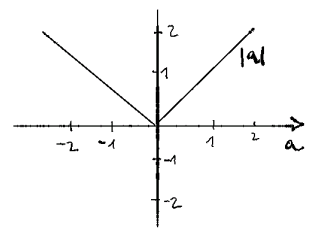
\includegraphics[width=0.4\textwidth]{betrag.png}
    \caption{Der Verlauf der $db_{FS}$ Kurve.}
    \label{fig:dbfs}
\end{figure}


\begin{figure}[h!]
    \centering
    %% Creator: Matplotlib, PGF backend
%%
%% To include the figure in your LaTeX document, write
%%   \input{<filename>.pgf}
%%
%% Make sure the required packages are loaded in your preamble
%%   \usepackage{pgf}
%%
%% Also ensure that all the required font packages are loaded; for instance,
%% the lmodern package is sometimes necessary when using math font.
%%   \usepackage{lmodern}
%%
%% Figures using additional raster images can only be included by \input if
%% they are in the same directory as the main LaTeX file. For loading figures
%% from other directories you can use the `import` package
%%   \usepackage{import}
%%
%% and then include the figures with
%%   \import{<path to file>}{<filename>.pgf}
%%
%% Matplotlib used the following preamble
%%   \def\mathdefault#1{#1}
%%   \everymath=\expandafter{\the\everymath\displaystyle}
%%   
%%   \usepackage{fontspec}
%%   \setmainfont{VeraSe.ttf}[Path=\detokenize{/usr/share/fonts/TTF/}]
%%   \setsansfont{DejaVuSans.ttf}[Path=\detokenize{/home/pl/miniconda3/lib/python3.12/site-packages/matplotlib/mpl-data/fonts/ttf/}]
%%   \setmonofont{DejaVuSansMono.ttf}[Path=\detokenize{/home/pl/miniconda3/lib/python3.12/site-packages/matplotlib/mpl-data/fonts/ttf/}]
%%   \makeatletter\@ifpackageloaded{underscore}{}{\usepackage[strings]{underscore}}\makeatother
%%
\begingroup%
\makeatletter%
\begin{pgfpicture}%
\pgfpathrectangle{\pgfpointorigin}{\pgfqpoint{6.340780in}{3.166819in}}%
\pgfusepath{use as bounding box, clip}%
\begin{pgfscope}%
\pgfsetbuttcap%
\pgfsetmiterjoin%
\definecolor{currentfill}{rgb}{1.000000,1.000000,1.000000}%
\pgfsetfillcolor{currentfill}%
\pgfsetlinewidth{0.000000pt}%
\definecolor{currentstroke}{rgb}{1.000000,1.000000,1.000000}%
\pgfsetstrokecolor{currentstroke}%
\pgfsetdash{}{0pt}%
\pgfpathmoveto{\pgfqpoint{0.000000in}{0.000000in}}%
\pgfpathlineto{\pgfqpoint{6.340780in}{0.000000in}}%
\pgfpathlineto{\pgfqpoint{6.340780in}{3.166819in}}%
\pgfpathlineto{\pgfqpoint{0.000000in}{3.166819in}}%
\pgfpathlineto{\pgfqpoint{0.000000in}{0.000000in}}%
\pgfpathclose%
\pgfusepath{fill}%
\end{pgfscope}%
\begin{pgfscope}%
\pgfsetbuttcap%
\pgfsetmiterjoin%
\definecolor{currentfill}{rgb}{1.000000,1.000000,1.000000}%
\pgfsetfillcolor{currentfill}%
\pgfsetlinewidth{0.000000pt}%
\definecolor{currentstroke}{rgb}{0.000000,0.000000,0.000000}%
\pgfsetstrokecolor{currentstroke}%
\pgfsetstrokeopacity{0.000000}%
\pgfsetdash{}{0pt}%
\pgfpathmoveto{\pgfqpoint{0.639049in}{0.548486in}}%
\pgfpathlineto{\pgfqpoint{3.104958in}{0.548486in}}%
\pgfpathlineto{\pgfqpoint{3.104958in}{2.858486in}}%
\pgfpathlineto{\pgfqpoint{0.639049in}{2.858486in}}%
\pgfpathlineto{\pgfqpoint{0.639049in}{0.548486in}}%
\pgfpathclose%
\pgfusepath{fill}%
\end{pgfscope}%
\begin{pgfscope}%
\pgfsetbuttcap%
\pgfsetroundjoin%
\definecolor{currentfill}{rgb}{0.000000,0.000000,0.000000}%
\pgfsetfillcolor{currentfill}%
\pgfsetlinewidth{0.803000pt}%
\definecolor{currentstroke}{rgb}{0.000000,0.000000,0.000000}%
\pgfsetstrokecolor{currentstroke}%
\pgfsetdash{}{0pt}%
\pgfsys@defobject{currentmarker}{\pgfqpoint{0.000000in}{-0.048611in}}{\pgfqpoint{0.000000in}{0.000000in}}{%
\pgfpathmoveto{\pgfqpoint{0.000000in}{0.000000in}}%
\pgfpathlineto{\pgfqpoint{0.000000in}{-0.048611in}}%
\pgfusepath{stroke,fill}%
}%
\begin{pgfscope}%
\pgfsys@transformshift{0.639049in}{0.548486in}%
\pgfsys@useobject{currentmarker}{}%
\end{pgfscope}%
\end{pgfscope}%
\begin{pgfscope}%
\definecolor{textcolor}{rgb}{0.000000,0.000000,0.000000}%
\pgfsetstrokecolor{textcolor}%
\pgfsetfillcolor{textcolor}%
\pgftext[x=0.639049in,y=0.451264in,,top]{\color{textcolor}{\rmfamily\fontsize{10.000000}{12.000000}\selectfont\catcode`\^=\active\def^{\ifmmode\sp\else\^{}\fi}\catcode`\%=\active\def%{\%}0}}%
\end{pgfscope}%
\begin{pgfscope}%
\pgfsetbuttcap%
\pgfsetroundjoin%
\definecolor{currentfill}{rgb}{0.000000,0.000000,0.000000}%
\pgfsetfillcolor{currentfill}%
\pgfsetlinewidth{0.803000pt}%
\definecolor{currentstroke}{rgb}{0.000000,0.000000,0.000000}%
\pgfsetstrokecolor{currentstroke}%
\pgfsetdash{}{0pt}%
\pgfsys@defobject{currentmarker}{\pgfqpoint{0.000000in}{-0.048611in}}{\pgfqpoint{0.000000in}{0.000000in}}{%
\pgfpathmoveto{\pgfqpoint{0.000000in}{0.000000in}}%
\pgfpathlineto{\pgfqpoint{0.000000in}{-0.048611in}}%
\pgfusepath{stroke,fill}%
}%
\begin{pgfscope}%
\pgfsys@transformshift{1.255526in}{0.548486in}%
\pgfsys@useobject{currentmarker}{}%
\end{pgfscope}%
\end{pgfscope}%
\begin{pgfscope}%
\definecolor{textcolor}{rgb}{0.000000,0.000000,0.000000}%
\pgfsetstrokecolor{textcolor}%
\pgfsetfillcolor{textcolor}%
\pgftext[x=1.255526in,y=0.451264in,,top]{\color{textcolor}{\rmfamily\fontsize{10.000000}{12.000000}\selectfont\catcode`\^=\active\def^{\ifmmode\sp\else\^{}\fi}\catcode`\%=\active\def%{\%}500}}%
\end{pgfscope}%
\begin{pgfscope}%
\pgfsetbuttcap%
\pgfsetroundjoin%
\definecolor{currentfill}{rgb}{0.000000,0.000000,0.000000}%
\pgfsetfillcolor{currentfill}%
\pgfsetlinewidth{0.803000pt}%
\definecolor{currentstroke}{rgb}{0.000000,0.000000,0.000000}%
\pgfsetstrokecolor{currentstroke}%
\pgfsetdash{}{0pt}%
\pgfsys@defobject{currentmarker}{\pgfqpoint{0.000000in}{-0.048611in}}{\pgfqpoint{0.000000in}{0.000000in}}{%
\pgfpathmoveto{\pgfqpoint{0.000000in}{0.000000in}}%
\pgfpathlineto{\pgfqpoint{0.000000in}{-0.048611in}}%
\pgfusepath{stroke,fill}%
}%
\begin{pgfscope}%
\pgfsys@transformshift{1.872003in}{0.548486in}%
\pgfsys@useobject{currentmarker}{}%
\end{pgfscope}%
\end{pgfscope}%
\begin{pgfscope}%
\definecolor{textcolor}{rgb}{0.000000,0.000000,0.000000}%
\pgfsetstrokecolor{textcolor}%
\pgfsetfillcolor{textcolor}%
\pgftext[x=1.872003in,y=0.451264in,,top]{\color{textcolor}{\rmfamily\fontsize{10.000000}{12.000000}\selectfont\catcode`\^=\active\def^{\ifmmode\sp\else\^{}\fi}\catcode`\%=\active\def%{\%}1000}}%
\end{pgfscope}%
\begin{pgfscope}%
\pgfsetbuttcap%
\pgfsetroundjoin%
\definecolor{currentfill}{rgb}{0.000000,0.000000,0.000000}%
\pgfsetfillcolor{currentfill}%
\pgfsetlinewidth{0.803000pt}%
\definecolor{currentstroke}{rgb}{0.000000,0.000000,0.000000}%
\pgfsetstrokecolor{currentstroke}%
\pgfsetdash{}{0pt}%
\pgfsys@defobject{currentmarker}{\pgfqpoint{0.000000in}{-0.048611in}}{\pgfqpoint{0.000000in}{0.000000in}}{%
\pgfpathmoveto{\pgfqpoint{0.000000in}{0.000000in}}%
\pgfpathlineto{\pgfqpoint{0.000000in}{-0.048611in}}%
\pgfusepath{stroke,fill}%
}%
\begin{pgfscope}%
\pgfsys@transformshift{2.488481in}{0.548486in}%
\pgfsys@useobject{currentmarker}{}%
\end{pgfscope}%
\end{pgfscope}%
\begin{pgfscope}%
\definecolor{textcolor}{rgb}{0.000000,0.000000,0.000000}%
\pgfsetstrokecolor{textcolor}%
\pgfsetfillcolor{textcolor}%
\pgftext[x=2.488481in,y=0.451264in,,top]{\color{textcolor}{\rmfamily\fontsize{10.000000}{12.000000}\selectfont\catcode`\^=\active\def^{\ifmmode\sp\else\^{}\fi}\catcode`\%=\active\def%{\%}1500}}%
\end{pgfscope}%
\begin{pgfscope}%
\pgfsetbuttcap%
\pgfsetroundjoin%
\definecolor{currentfill}{rgb}{0.000000,0.000000,0.000000}%
\pgfsetfillcolor{currentfill}%
\pgfsetlinewidth{0.803000pt}%
\definecolor{currentstroke}{rgb}{0.000000,0.000000,0.000000}%
\pgfsetstrokecolor{currentstroke}%
\pgfsetdash{}{0pt}%
\pgfsys@defobject{currentmarker}{\pgfqpoint{0.000000in}{-0.048611in}}{\pgfqpoint{0.000000in}{0.000000in}}{%
\pgfpathmoveto{\pgfqpoint{0.000000in}{0.000000in}}%
\pgfpathlineto{\pgfqpoint{0.000000in}{-0.048611in}}%
\pgfusepath{stroke,fill}%
}%
\begin{pgfscope}%
\pgfsys@transformshift{3.104958in}{0.548486in}%
\pgfsys@useobject{currentmarker}{}%
\end{pgfscope}%
\end{pgfscope}%
\begin{pgfscope}%
\definecolor{textcolor}{rgb}{0.000000,0.000000,0.000000}%
\pgfsetstrokecolor{textcolor}%
\pgfsetfillcolor{textcolor}%
\pgftext[x=3.104958in,y=0.451264in,,top]{\color{textcolor}{\rmfamily\fontsize{10.000000}{12.000000}\selectfont\catcode`\^=\active\def^{\ifmmode\sp\else\^{}\fi}\catcode`\%=\active\def%{\%}2000}}%
\end{pgfscope}%
\begin{pgfscope}%
\definecolor{textcolor}{rgb}{0.000000,0.000000,0.000000}%
\pgfsetstrokecolor{textcolor}%
\pgfsetfillcolor{textcolor}%
\pgftext[x=1.872003in,y=0.261295in,,top]{\color{textcolor}{\rmfamily\fontsize{12.000000}{14.400000}\selectfont\catcode`\^=\active\def^{\ifmmode\sp\else\^{}\fi}\catcode`\%=\active\def%{\%}f [Hz]}}%
\end{pgfscope}%
\begin{pgfscope}%
\pgfsetbuttcap%
\pgfsetroundjoin%
\definecolor{currentfill}{rgb}{0.000000,0.000000,0.000000}%
\pgfsetfillcolor{currentfill}%
\pgfsetlinewidth{0.803000pt}%
\definecolor{currentstroke}{rgb}{0.000000,0.000000,0.000000}%
\pgfsetstrokecolor{currentstroke}%
\pgfsetdash{}{0pt}%
\pgfsys@defobject{currentmarker}{\pgfqpoint{-0.048611in}{0.000000in}}{\pgfqpoint{-0.000000in}{0.000000in}}{%
\pgfpathmoveto{\pgfqpoint{-0.000000in}{0.000000in}}%
\pgfpathlineto{\pgfqpoint{-0.048611in}{0.000000in}}%
\pgfusepath{stroke,fill}%
}%
\begin{pgfscope}%
\pgfsys@transformshift{0.639049in}{1.010485in}%
\pgfsys@useobject{currentmarker}{}%
\end{pgfscope}%
\end{pgfscope}%
\begin{pgfscope}%
\definecolor{textcolor}{rgb}{0.000000,0.000000,0.000000}%
\pgfsetstrokecolor{textcolor}%
\pgfsetfillcolor{textcolor}%
\pgftext[x=0.188365in, y=0.957724in, left, base]{\color{textcolor}{\rmfamily\fontsize{10.000000}{12.000000}\selectfont\catcode`\^=\active\def^{\ifmmode\sp\else\^{}\fi}\catcode`\%=\active\def%{\%}2000}}%
\end{pgfscope}%
\begin{pgfscope}%
\pgfsetbuttcap%
\pgfsetroundjoin%
\definecolor{currentfill}{rgb}{0.000000,0.000000,0.000000}%
\pgfsetfillcolor{currentfill}%
\pgfsetlinewidth{0.803000pt}%
\definecolor{currentstroke}{rgb}{0.000000,0.000000,0.000000}%
\pgfsetstrokecolor{currentstroke}%
\pgfsetdash{}{0pt}%
\pgfsys@defobject{currentmarker}{\pgfqpoint{-0.048611in}{0.000000in}}{\pgfqpoint{-0.000000in}{0.000000in}}{%
\pgfpathmoveto{\pgfqpoint{-0.000000in}{0.000000in}}%
\pgfpathlineto{\pgfqpoint{-0.048611in}{0.000000in}}%
\pgfusepath{stroke,fill}%
}%
\begin{pgfscope}%
\pgfsys@transformshift{0.639049in}{1.472486in}%
\pgfsys@useobject{currentmarker}{}%
\end{pgfscope}%
\end{pgfscope}%
\begin{pgfscope}%
\definecolor{textcolor}{rgb}{0.000000,0.000000,0.000000}%
\pgfsetstrokecolor{textcolor}%
\pgfsetfillcolor{textcolor}%
\pgftext[x=0.188365in, y=1.419724in, left, base]{\color{textcolor}{\rmfamily\fontsize{10.000000}{12.000000}\selectfont\catcode`\^=\active\def^{\ifmmode\sp\else\^{}\fi}\catcode`\%=\active\def%{\%}4000}}%
\end{pgfscope}%
\begin{pgfscope}%
\pgfsetbuttcap%
\pgfsetroundjoin%
\definecolor{currentfill}{rgb}{0.000000,0.000000,0.000000}%
\pgfsetfillcolor{currentfill}%
\pgfsetlinewidth{0.803000pt}%
\definecolor{currentstroke}{rgb}{0.000000,0.000000,0.000000}%
\pgfsetstrokecolor{currentstroke}%
\pgfsetdash{}{0pt}%
\pgfsys@defobject{currentmarker}{\pgfqpoint{-0.048611in}{0.000000in}}{\pgfqpoint{-0.000000in}{0.000000in}}{%
\pgfpathmoveto{\pgfqpoint{-0.000000in}{0.000000in}}%
\pgfpathlineto{\pgfqpoint{-0.048611in}{0.000000in}}%
\pgfusepath{stroke,fill}%
}%
\begin{pgfscope}%
\pgfsys@transformshift{0.639049in}{1.934486in}%
\pgfsys@useobject{currentmarker}{}%
\end{pgfscope}%
\end{pgfscope}%
\begin{pgfscope}%
\definecolor{textcolor}{rgb}{0.000000,0.000000,0.000000}%
\pgfsetstrokecolor{textcolor}%
\pgfsetfillcolor{textcolor}%
\pgftext[x=0.188365in, y=1.881724in, left, base]{\color{textcolor}{\rmfamily\fontsize{10.000000}{12.000000}\selectfont\catcode`\^=\active\def^{\ifmmode\sp\else\^{}\fi}\catcode`\%=\active\def%{\%}6000}}%
\end{pgfscope}%
\begin{pgfscope}%
\pgfsetbuttcap%
\pgfsetroundjoin%
\definecolor{currentfill}{rgb}{0.000000,0.000000,0.000000}%
\pgfsetfillcolor{currentfill}%
\pgfsetlinewidth{0.803000pt}%
\definecolor{currentstroke}{rgb}{0.000000,0.000000,0.000000}%
\pgfsetstrokecolor{currentstroke}%
\pgfsetdash{}{0pt}%
\pgfsys@defobject{currentmarker}{\pgfqpoint{-0.048611in}{0.000000in}}{\pgfqpoint{-0.000000in}{0.000000in}}{%
\pgfpathmoveto{\pgfqpoint{-0.000000in}{0.000000in}}%
\pgfpathlineto{\pgfqpoint{-0.048611in}{0.000000in}}%
\pgfusepath{stroke,fill}%
}%
\begin{pgfscope}%
\pgfsys@transformshift{0.639049in}{2.396486in}%
\pgfsys@useobject{currentmarker}{}%
\end{pgfscope}%
\end{pgfscope}%
\begin{pgfscope}%
\definecolor{textcolor}{rgb}{0.000000,0.000000,0.000000}%
\pgfsetstrokecolor{textcolor}%
\pgfsetfillcolor{textcolor}%
\pgftext[x=0.188365in, y=2.343724in, left, base]{\color{textcolor}{\rmfamily\fontsize{10.000000}{12.000000}\selectfont\catcode`\^=\active\def^{\ifmmode\sp\else\^{}\fi}\catcode`\%=\active\def%{\%}8000}}%
\end{pgfscope}%
\begin{pgfscope}%
\pgfsetbuttcap%
\pgfsetroundjoin%
\definecolor{currentfill}{rgb}{0.000000,0.000000,0.000000}%
\pgfsetfillcolor{currentfill}%
\pgfsetlinewidth{0.803000pt}%
\definecolor{currentstroke}{rgb}{0.000000,0.000000,0.000000}%
\pgfsetstrokecolor{currentstroke}%
\pgfsetdash{}{0pt}%
\pgfsys@defobject{currentmarker}{\pgfqpoint{-0.048611in}{0.000000in}}{\pgfqpoint{-0.000000in}{0.000000in}}{%
\pgfpathmoveto{\pgfqpoint{-0.000000in}{0.000000in}}%
\pgfpathlineto{\pgfqpoint{-0.048611in}{0.000000in}}%
\pgfusepath{stroke,fill}%
}%
\begin{pgfscope}%
\pgfsys@transformshift{0.639049in}{2.858486in}%
\pgfsys@useobject{currentmarker}{}%
\end{pgfscope}%
\end{pgfscope}%
\begin{pgfscope}%
\definecolor{textcolor}{rgb}{0.000000,0.000000,0.000000}%
\pgfsetstrokecolor{textcolor}%
\pgfsetfillcolor{textcolor}%
\pgftext[x=0.100000in, y=2.805724in, left, base]{\color{textcolor}{\rmfamily\fontsize{10.000000}{12.000000}\selectfont\catcode`\^=\active\def^{\ifmmode\sp\else\^{}\fi}\catcode`\%=\active\def%{\%}10000}}%
\end{pgfscope}%
\begin{pgfscope}%
\pgfpathrectangle{\pgfqpoint{0.639049in}{0.548486in}}{\pgfqpoint{2.465909in}{2.310000in}}%
\pgfusepath{clip}%
\pgfsetrectcap%
\pgfsetroundjoin%
\pgfsetlinewidth{1.505625pt}%
\definecolor{currentstroke}{rgb}{0.000000,0.000000,0.000000}%
\pgfsetstrokecolor{currentstroke}%
\pgfsetdash{}{0pt}%
\pgfpathmoveto{\pgfqpoint{0.637816in}{0.548488in}}%
\pgfpathlineto{\pgfqpoint{0.742617in}{0.549304in}}%
\pgfpathlineto{\pgfqpoint{0.754947in}{0.550755in}}%
\pgfpathlineto{\pgfqpoint{0.758645in}{0.553054in}}%
\pgfpathlineto{\pgfqpoint{0.759878in}{0.555334in}}%
\pgfpathlineto{\pgfqpoint{0.761111in}{0.562072in}}%
\pgfpathlineto{\pgfqpoint{0.762344in}{1.162913in}}%
\pgfpathlineto{\pgfqpoint{0.763577in}{0.562784in}}%
\pgfpathlineto{\pgfqpoint{0.766043in}{0.553204in}}%
\pgfpathlineto{\pgfqpoint{0.769742in}{0.550852in}}%
\pgfpathlineto{\pgfqpoint{0.778373in}{0.549590in}}%
\pgfpathlineto{\pgfqpoint{0.806731in}{0.548887in}}%
\pgfpathlineto{\pgfqpoint{0.959617in}{0.548605in}}%
\pgfpathlineto{\pgfqpoint{1.000305in}{0.549766in}}%
\pgfpathlineto{\pgfqpoint{1.005236in}{0.551571in}}%
\pgfpathlineto{\pgfqpoint{1.006469in}{0.553111in}}%
\pgfpathlineto{\pgfqpoint{1.007702in}{0.557535in}}%
\pgfpathlineto{\pgfqpoint{1.008935in}{0.691956in}}%
\pgfpathlineto{\pgfqpoint{1.010168in}{0.559063in}}%
\pgfpathlineto{\pgfqpoint{1.012634in}{0.551912in}}%
\pgfpathlineto{\pgfqpoint{1.016333in}{0.550225in}}%
\pgfpathlineto{\pgfqpoint{1.026197in}{0.549274in}}%
\pgfpathlineto{\pgfqpoint{1.068117in}{0.548757in}}%
\pgfpathlineto{\pgfqpoint{1.246895in}{0.549144in}}%
\pgfpathlineto{\pgfqpoint{1.251827in}{0.550142in}}%
\pgfpathlineto{\pgfqpoint{1.253060in}{0.550980in}}%
\pgfpathlineto{\pgfqpoint{1.254293in}{0.553324in}}%
\pgfpathlineto{\pgfqpoint{1.255526in}{0.596997in}}%
\pgfpathlineto{\pgfqpoint{1.256759in}{0.554818in}}%
\pgfpathlineto{\pgfqpoint{1.259225in}{0.550507in}}%
\pgfpathlineto{\pgfqpoint{1.264157in}{0.549396in}}%
\pgfpathlineto{\pgfqpoint{1.283884in}{0.548829in}}%
\pgfpathlineto{\pgfqpoint{1.446634in}{0.548547in}}%
\pgfpathlineto{\pgfqpoint{1.498418in}{0.549243in}}%
\pgfpathlineto{\pgfqpoint{1.500884in}{0.550738in}}%
\pgfpathlineto{\pgfqpoint{1.502117in}{0.565599in}}%
\pgfpathlineto{\pgfqpoint{1.504583in}{0.550076in}}%
\pgfpathlineto{\pgfqpoint{1.509515in}{0.549058in}}%
\pgfpathlineto{\pgfqpoint{1.535407in}{0.548686in}}%
\pgfpathlineto{\pgfqpoint{1.746242in}{0.548959in}}%
\pgfpathlineto{\pgfqpoint{1.747475in}{0.549430in}}%
\pgfpathlineto{\pgfqpoint{1.748708in}{0.554510in}}%
\pgfpathlineto{\pgfqpoint{1.751174in}{0.549272in}}%
\pgfpathlineto{\pgfqpoint{1.758572in}{0.548736in}}%
\pgfpathlineto{\pgfqpoint{1.842413in}{0.548582in}}%
\pgfpathlineto{\pgfqpoint{1.994066in}{0.548838in}}%
\pgfpathlineto{\pgfqpoint{1.995299in}{0.550568in}}%
\pgfpathlineto{\pgfqpoint{1.997765in}{0.548872in}}%
\pgfpathlineto{\pgfqpoint{2.012560in}{0.548602in}}%
\pgfpathlineto{\pgfqpoint{2.487248in}{0.548491in}}%
\pgfpathlineto{\pgfqpoint{2.494645in}{0.548565in}}%
\pgfpathlineto{\pgfqpoint{2.901520in}{0.548539in}}%
\pgfpathlineto{\pgfqpoint{3.106191in}{0.548537in}}%
\pgfpathlineto{\pgfqpoint{3.106191in}{0.548537in}}%
\pgfusepath{stroke}%
\end{pgfscope}%
\begin{pgfscope}%
\definecolor{textcolor}{rgb}{0.000000,0.000000,0.000000}%
\pgfsetstrokecolor{textcolor}%
\pgfsetfillcolor{textcolor}%
\pgftext[x=1.872003in,y=2.941819in,,base]{\color{textcolor}{\rmfamily\fontsize{12.000000}{14.400000}\selectfont\catcode`\^=\active\def^{\ifmmode\sp\else\^{}\fi}\catcode`\%=\active\def%{\%}$|X(f)|$}}%
\end{pgfscope}%
\begin{pgfscope}%
\pgfsetbuttcap%
\pgfsetmiterjoin%
\definecolor{currentfill}{rgb}{1.000000,1.000000,1.000000}%
\pgfsetfillcolor{currentfill}%
\pgfsetlinewidth{0.000000pt}%
\definecolor{currentstroke}{rgb}{0.000000,0.000000,0.000000}%
\pgfsetstrokecolor{currentstroke}%
\pgfsetstrokeopacity{0.000000}%
\pgfsetdash{}{0pt}%
\pgfpathmoveto{\pgfqpoint{3.598140in}{0.548486in}}%
\pgfpathlineto{\pgfqpoint{6.064049in}{0.548486in}}%
\pgfpathlineto{\pgfqpoint{6.064049in}{2.858486in}}%
\pgfpathlineto{\pgfqpoint{3.598140in}{2.858486in}}%
\pgfpathlineto{\pgfqpoint{3.598140in}{0.548486in}}%
\pgfpathclose%
\pgfusepath{fill}%
\end{pgfscope}%
\begin{pgfscope}%
\pgfsetbuttcap%
\pgfsetroundjoin%
\definecolor{currentfill}{rgb}{0.000000,0.000000,0.000000}%
\pgfsetfillcolor{currentfill}%
\pgfsetlinewidth{0.803000pt}%
\definecolor{currentstroke}{rgb}{0.000000,0.000000,0.000000}%
\pgfsetstrokecolor{currentstroke}%
\pgfsetdash{}{0pt}%
\pgfsys@defobject{currentmarker}{\pgfqpoint{0.000000in}{-0.048611in}}{\pgfqpoint{0.000000in}{0.000000in}}{%
\pgfpathmoveto{\pgfqpoint{0.000000in}{0.000000in}}%
\pgfpathlineto{\pgfqpoint{0.000000in}{-0.048611in}}%
\pgfusepath{stroke,fill}%
}%
\begin{pgfscope}%
\pgfsys@transformshift{3.598140in}{0.548486in}%
\pgfsys@useobject{currentmarker}{}%
\end{pgfscope}%
\end{pgfscope}%
\begin{pgfscope}%
\definecolor{textcolor}{rgb}{0.000000,0.000000,0.000000}%
\pgfsetstrokecolor{textcolor}%
\pgfsetfillcolor{textcolor}%
\pgftext[x=3.598140in,y=0.451264in,,top]{\color{textcolor}{\rmfamily\fontsize{10.000000}{12.000000}\selectfont\catcode`\^=\active\def^{\ifmmode\sp\else\^{}\fi}\catcode`\%=\active\def%{\%}0}}%
\end{pgfscope}%
\begin{pgfscope}%
\pgfsetbuttcap%
\pgfsetroundjoin%
\definecolor{currentfill}{rgb}{0.000000,0.000000,0.000000}%
\pgfsetfillcolor{currentfill}%
\pgfsetlinewidth{0.803000pt}%
\definecolor{currentstroke}{rgb}{0.000000,0.000000,0.000000}%
\pgfsetstrokecolor{currentstroke}%
\pgfsetdash{}{0pt}%
\pgfsys@defobject{currentmarker}{\pgfqpoint{0.000000in}{-0.048611in}}{\pgfqpoint{0.000000in}{0.000000in}}{%
\pgfpathmoveto{\pgfqpoint{0.000000in}{0.000000in}}%
\pgfpathlineto{\pgfqpoint{0.000000in}{-0.048611in}}%
\pgfusepath{stroke,fill}%
}%
\begin{pgfscope}%
\pgfsys@transformshift{4.214617in}{0.548486in}%
\pgfsys@useobject{currentmarker}{}%
\end{pgfscope}%
\end{pgfscope}%
\begin{pgfscope}%
\definecolor{textcolor}{rgb}{0.000000,0.000000,0.000000}%
\pgfsetstrokecolor{textcolor}%
\pgfsetfillcolor{textcolor}%
\pgftext[x=4.214617in,y=0.451264in,,top]{\color{textcolor}{\rmfamily\fontsize{10.000000}{12.000000}\selectfont\catcode`\^=\active\def^{\ifmmode\sp\else\^{}\fi}\catcode`\%=\active\def%{\%}500}}%
\end{pgfscope}%
\begin{pgfscope}%
\pgfsetbuttcap%
\pgfsetroundjoin%
\definecolor{currentfill}{rgb}{0.000000,0.000000,0.000000}%
\pgfsetfillcolor{currentfill}%
\pgfsetlinewidth{0.803000pt}%
\definecolor{currentstroke}{rgb}{0.000000,0.000000,0.000000}%
\pgfsetstrokecolor{currentstroke}%
\pgfsetdash{}{0pt}%
\pgfsys@defobject{currentmarker}{\pgfqpoint{0.000000in}{-0.048611in}}{\pgfqpoint{0.000000in}{0.000000in}}{%
\pgfpathmoveto{\pgfqpoint{0.000000in}{0.000000in}}%
\pgfpathlineto{\pgfqpoint{0.000000in}{-0.048611in}}%
\pgfusepath{stroke,fill}%
}%
\begin{pgfscope}%
\pgfsys@transformshift{4.831094in}{0.548486in}%
\pgfsys@useobject{currentmarker}{}%
\end{pgfscope}%
\end{pgfscope}%
\begin{pgfscope}%
\definecolor{textcolor}{rgb}{0.000000,0.000000,0.000000}%
\pgfsetstrokecolor{textcolor}%
\pgfsetfillcolor{textcolor}%
\pgftext[x=4.831094in,y=0.451264in,,top]{\color{textcolor}{\rmfamily\fontsize{10.000000}{12.000000}\selectfont\catcode`\^=\active\def^{\ifmmode\sp\else\^{}\fi}\catcode`\%=\active\def%{\%}1000}}%
\end{pgfscope}%
\begin{pgfscope}%
\pgfsetbuttcap%
\pgfsetroundjoin%
\definecolor{currentfill}{rgb}{0.000000,0.000000,0.000000}%
\pgfsetfillcolor{currentfill}%
\pgfsetlinewidth{0.803000pt}%
\definecolor{currentstroke}{rgb}{0.000000,0.000000,0.000000}%
\pgfsetstrokecolor{currentstroke}%
\pgfsetdash{}{0pt}%
\pgfsys@defobject{currentmarker}{\pgfqpoint{0.000000in}{-0.048611in}}{\pgfqpoint{0.000000in}{0.000000in}}{%
\pgfpathmoveto{\pgfqpoint{0.000000in}{0.000000in}}%
\pgfpathlineto{\pgfqpoint{0.000000in}{-0.048611in}}%
\pgfusepath{stroke,fill}%
}%
\begin{pgfscope}%
\pgfsys@transformshift{5.447572in}{0.548486in}%
\pgfsys@useobject{currentmarker}{}%
\end{pgfscope}%
\end{pgfscope}%
\begin{pgfscope}%
\definecolor{textcolor}{rgb}{0.000000,0.000000,0.000000}%
\pgfsetstrokecolor{textcolor}%
\pgfsetfillcolor{textcolor}%
\pgftext[x=5.447572in,y=0.451264in,,top]{\color{textcolor}{\rmfamily\fontsize{10.000000}{12.000000}\selectfont\catcode`\^=\active\def^{\ifmmode\sp\else\^{}\fi}\catcode`\%=\active\def%{\%}1500}}%
\end{pgfscope}%
\begin{pgfscope}%
\pgfsetbuttcap%
\pgfsetroundjoin%
\definecolor{currentfill}{rgb}{0.000000,0.000000,0.000000}%
\pgfsetfillcolor{currentfill}%
\pgfsetlinewidth{0.803000pt}%
\definecolor{currentstroke}{rgb}{0.000000,0.000000,0.000000}%
\pgfsetstrokecolor{currentstroke}%
\pgfsetdash{}{0pt}%
\pgfsys@defobject{currentmarker}{\pgfqpoint{0.000000in}{-0.048611in}}{\pgfqpoint{0.000000in}{0.000000in}}{%
\pgfpathmoveto{\pgfqpoint{0.000000in}{0.000000in}}%
\pgfpathlineto{\pgfqpoint{0.000000in}{-0.048611in}}%
\pgfusepath{stroke,fill}%
}%
\begin{pgfscope}%
\pgfsys@transformshift{6.064049in}{0.548486in}%
\pgfsys@useobject{currentmarker}{}%
\end{pgfscope}%
\end{pgfscope}%
\begin{pgfscope}%
\definecolor{textcolor}{rgb}{0.000000,0.000000,0.000000}%
\pgfsetstrokecolor{textcolor}%
\pgfsetfillcolor{textcolor}%
\pgftext[x=6.064049in,y=0.451264in,,top]{\color{textcolor}{\rmfamily\fontsize{10.000000}{12.000000}\selectfont\catcode`\^=\active\def^{\ifmmode\sp\else\^{}\fi}\catcode`\%=\active\def%{\%}2000}}%
\end{pgfscope}%
\begin{pgfscope}%
\definecolor{textcolor}{rgb}{0.000000,0.000000,0.000000}%
\pgfsetstrokecolor{textcolor}%
\pgfsetfillcolor{textcolor}%
\pgftext[x=4.831094in,y=0.261295in,,top]{\color{textcolor}{\rmfamily\fontsize{12.000000}{14.400000}\selectfont\catcode`\^=\active\def^{\ifmmode\sp\else\^{}\fi}\catcode`\%=\active\def%{\%}f [Hz]}}%
\end{pgfscope}%
\begin{pgfscope}%
\pgfsetbuttcap%
\pgfsetroundjoin%
\definecolor{currentfill}{rgb}{0.000000,0.000000,0.000000}%
\pgfsetfillcolor{currentfill}%
\pgfsetlinewidth{0.803000pt}%
\definecolor{currentstroke}{rgb}{0.000000,0.000000,0.000000}%
\pgfsetstrokecolor{currentstroke}%
\pgfsetdash{}{0pt}%
\pgfsys@defobject{currentmarker}{\pgfqpoint{-0.048611in}{0.000000in}}{\pgfqpoint{-0.000000in}{0.000000in}}{%
\pgfpathmoveto{\pgfqpoint{-0.000000in}{0.000000in}}%
\pgfpathlineto{\pgfqpoint{-0.048611in}{0.000000in}}%
\pgfusepath{stroke,fill}%
}%
\begin{pgfscope}%
\pgfsys@transformshift{3.598140in}{0.726178in}%
\pgfsys@useobject{currentmarker}{}%
\end{pgfscope}%
\end{pgfscope}%
\begin{pgfscope}%
\definecolor{textcolor}{rgb}{0.000000,0.000000,0.000000}%
\pgfsetstrokecolor{textcolor}%
\pgfsetfillcolor{textcolor}%
\pgftext[x=3.216162in, y=0.673417in, left, base]{\color{textcolor}{\rmfamily\fontsize{10.000000}{12.000000}\selectfont\catcode`\^=\active\def^{\ifmmode\sp\else\^{}\fi}\catcode`\%=\active\def%{\%}\ensuremath{-}40}}%
\end{pgfscope}%
\begin{pgfscope}%
\pgfsetbuttcap%
\pgfsetroundjoin%
\definecolor{currentfill}{rgb}{0.000000,0.000000,0.000000}%
\pgfsetfillcolor{currentfill}%
\pgfsetlinewidth{0.803000pt}%
\definecolor{currentstroke}{rgb}{0.000000,0.000000,0.000000}%
\pgfsetstrokecolor{currentstroke}%
\pgfsetdash{}{0pt}%
\pgfsys@defobject{currentmarker}{\pgfqpoint{-0.048611in}{0.000000in}}{\pgfqpoint{-0.000000in}{0.000000in}}{%
\pgfpathmoveto{\pgfqpoint{-0.000000in}{0.000000in}}%
\pgfpathlineto{\pgfqpoint{-0.048611in}{0.000000in}}%
\pgfusepath{stroke,fill}%
}%
\begin{pgfscope}%
\pgfsys@transformshift{3.598140in}{1.081563in}%
\pgfsys@useobject{currentmarker}{}%
\end{pgfscope}%
\end{pgfscope}%
\begin{pgfscope}%
\definecolor{textcolor}{rgb}{0.000000,0.000000,0.000000}%
\pgfsetstrokecolor{textcolor}%
\pgfsetfillcolor{textcolor}%
\pgftext[x=3.216162in, y=1.028801in, left, base]{\color{textcolor}{\rmfamily\fontsize{10.000000}{12.000000}\selectfont\catcode`\^=\active\def^{\ifmmode\sp\else\^{}\fi}\catcode`\%=\active\def%{\%}\ensuremath{-}20}}%
\end{pgfscope}%
\begin{pgfscope}%
\pgfsetbuttcap%
\pgfsetroundjoin%
\definecolor{currentfill}{rgb}{0.000000,0.000000,0.000000}%
\pgfsetfillcolor{currentfill}%
\pgfsetlinewidth{0.803000pt}%
\definecolor{currentstroke}{rgb}{0.000000,0.000000,0.000000}%
\pgfsetstrokecolor{currentstroke}%
\pgfsetdash{}{0pt}%
\pgfsys@defobject{currentmarker}{\pgfqpoint{-0.048611in}{0.000000in}}{\pgfqpoint{-0.000000in}{0.000000in}}{%
\pgfpathmoveto{\pgfqpoint{-0.000000in}{0.000000in}}%
\pgfpathlineto{\pgfqpoint{-0.048611in}{0.000000in}}%
\pgfusepath{stroke,fill}%
}%
\begin{pgfscope}%
\pgfsys@transformshift{3.598140in}{1.436948in}%
\pgfsys@useobject{currentmarker}{}%
\end{pgfscope}%
\end{pgfscope}%
\begin{pgfscope}%
\definecolor{textcolor}{rgb}{0.000000,0.000000,0.000000}%
\pgfsetstrokecolor{textcolor}%
\pgfsetfillcolor{textcolor}%
\pgftext[x=3.412552in, y=1.384186in, left, base]{\color{textcolor}{\rmfamily\fontsize{10.000000}{12.000000}\selectfont\catcode`\^=\active\def^{\ifmmode\sp\else\^{}\fi}\catcode`\%=\active\def%{\%}0}}%
\end{pgfscope}%
\begin{pgfscope}%
\pgfsetbuttcap%
\pgfsetroundjoin%
\definecolor{currentfill}{rgb}{0.000000,0.000000,0.000000}%
\pgfsetfillcolor{currentfill}%
\pgfsetlinewidth{0.803000pt}%
\definecolor{currentstroke}{rgb}{0.000000,0.000000,0.000000}%
\pgfsetstrokecolor{currentstroke}%
\pgfsetdash{}{0pt}%
\pgfsys@defobject{currentmarker}{\pgfqpoint{-0.048611in}{0.000000in}}{\pgfqpoint{-0.000000in}{0.000000in}}{%
\pgfpathmoveto{\pgfqpoint{-0.000000in}{0.000000in}}%
\pgfpathlineto{\pgfqpoint{-0.048611in}{0.000000in}}%
\pgfusepath{stroke,fill}%
}%
\begin{pgfscope}%
\pgfsys@transformshift{3.598140in}{1.792332in}%
\pgfsys@useobject{currentmarker}{}%
\end{pgfscope}%
\end{pgfscope}%
\begin{pgfscope}%
\definecolor{textcolor}{rgb}{0.000000,0.000000,0.000000}%
\pgfsetstrokecolor{textcolor}%
\pgfsetfillcolor{textcolor}%
\pgftext[x=3.324187in, y=1.739571in, left, base]{\color{textcolor}{\rmfamily\fontsize{10.000000}{12.000000}\selectfont\catcode`\^=\active\def^{\ifmmode\sp\else\^{}\fi}\catcode`\%=\active\def%{\%}20}}%
\end{pgfscope}%
\begin{pgfscope}%
\pgfsetbuttcap%
\pgfsetroundjoin%
\definecolor{currentfill}{rgb}{0.000000,0.000000,0.000000}%
\pgfsetfillcolor{currentfill}%
\pgfsetlinewidth{0.803000pt}%
\definecolor{currentstroke}{rgb}{0.000000,0.000000,0.000000}%
\pgfsetstrokecolor{currentstroke}%
\pgfsetdash{}{0pt}%
\pgfsys@defobject{currentmarker}{\pgfqpoint{-0.048611in}{0.000000in}}{\pgfqpoint{-0.000000in}{0.000000in}}{%
\pgfpathmoveto{\pgfqpoint{-0.000000in}{0.000000in}}%
\pgfpathlineto{\pgfqpoint{-0.048611in}{0.000000in}}%
\pgfusepath{stroke,fill}%
}%
\begin{pgfscope}%
\pgfsys@transformshift{3.598140in}{2.147717in}%
\pgfsys@useobject{currentmarker}{}%
\end{pgfscope}%
\end{pgfscope}%
\begin{pgfscope}%
\definecolor{textcolor}{rgb}{0.000000,0.000000,0.000000}%
\pgfsetstrokecolor{textcolor}%
\pgfsetfillcolor{textcolor}%
\pgftext[x=3.324187in, y=2.094955in, left, base]{\color{textcolor}{\rmfamily\fontsize{10.000000}{12.000000}\selectfont\catcode`\^=\active\def^{\ifmmode\sp\else\^{}\fi}\catcode`\%=\active\def%{\%}40}}%
\end{pgfscope}%
\begin{pgfscope}%
\pgfsetbuttcap%
\pgfsetroundjoin%
\definecolor{currentfill}{rgb}{0.000000,0.000000,0.000000}%
\pgfsetfillcolor{currentfill}%
\pgfsetlinewidth{0.803000pt}%
\definecolor{currentstroke}{rgb}{0.000000,0.000000,0.000000}%
\pgfsetstrokecolor{currentstroke}%
\pgfsetdash{}{0pt}%
\pgfsys@defobject{currentmarker}{\pgfqpoint{-0.048611in}{0.000000in}}{\pgfqpoint{-0.000000in}{0.000000in}}{%
\pgfpathmoveto{\pgfqpoint{-0.000000in}{0.000000in}}%
\pgfpathlineto{\pgfqpoint{-0.048611in}{0.000000in}}%
\pgfusepath{stroke,fill}%
}%
\begin{pgfscope}%
\pgfsys@transformshift{3.598140in}{2.503101in}%
\pgfsys@useobject{currentmarker}{}%
\end{pgfscope}%
\end{pgfscope}%
\begin{pgfscope}%
\definecolor{textcolor}{rgb}{0.000000,0.000000,0.000000}%
\pgfsetstrokecolor{textcolor}%
\pgfsetfillcolor{textcolor}%
\pgftext[x=3.324187in, y=2.450340in, left, base]{\color{textcolor}{\rmfamily\fontsize{10.000000}{12.000000}\selectfont\catcode`\^=\active\def^{\ifmmode\sp\else\^{}\fi}\catcode`\%=\active\def%{\%}60}}%
\end{pgfscope}%
\begin{pgfscope}%
\pgfsetbuttcap%
\pgfsetroundjoin%
\definecolor{currentfill}{rgb}{0.000000,0.000000,0.000000}%
\pgfsetfillcolor{currentfill}%
\pgfsetlinewidth{0.803000pt}%
\definecolor{currentstroke}{rgb}{0.000000,0.000000,0.000000}%
\pgfsetstrokecolor{currentstroke}%
\pgfsetdash{}{0pt}%
\pgfsys@defobject{currentmarker}{\pgfqpoint{-0.048611in}{0.000000in}}{\pgfqpoint{-0.000000in}{0.000000in}}{%
\pgfpathmoveto{\pgfqpoint{-0.000000in}{0.000000in}}%
\pgfpathlineto{\pgfqpoint{-0.048611in}{0.000000in}}%
\pgfusepath{stroke,fill}%
}%
\begin{pgfscope}%
\pgfsys@transformshift{3.598140in}{2.858486in}%
\pgfsys@useobject{currentmarker}{}%
\end{pgfscope}%
\end{pgfscope}%
\begin{pgfscope}%
\definecolor{textcolor}{rgb}{0.000000,0.000000,0.000000}%
\pgfsetstrokecolor{textcolor}%
\pgfsetfillcolor{textcolor}%
\pgftext[x=3.324187in, y=2.805724in, left, base]{\color{textcolor}{\rmfamily\fontsize{10.000000}{12.000000}\selectfont\catcode`\^=\active\def^{\ifmmode\sp\else\^{}\fi}\catcode`\%=\active\def%{\%}80}}%
\end{pgfscope}%
\begin{pgfscope}%
\pgfpathrectangle{\pgfqpoint{3.598140in}{0.548486in}}{\pgfqpoint{2.465909in}{2.310000in}}%
\pgfusepath{clip}%
\pgfsetrectcap%
\pgfsetroundjoin%
\pgfsetlinewidth{1.505625pt}%
\definecolor{currentstroke}{rgb}{0.000000,0.000000,0.000000}%
\pgfsetstrokecolor{currentstroke}%
\pgfsetdash{}{0pt}%
\pgfpathmoveto{\pgfqpoint{3.596907in}{0.769421in}}%
\pgfpathlineto{\pgfqpoint{3.596991in}{0.538486in}}%
\pgfpathmoveto{\pgfqpoint{3.599288in}{0.538486in}}%
\pgfpathlineto{\pgfqpoint{3.599373in}{0.769421in}}%
\pgfpathlineto{\pgfqpoint{3.601839in}{0.939096in}}%
\pgfpathlineto{\pgfqpoint{3.605538in}{1.046462in}}%
\pgfpathlineto{\pgfqpoint{3.610469in}{1.126218in}}%
\pgfpathlineto{\pgfqpoint{3.616634in}{1.190604in}}%
\pgfpathlineto{\pgfqpoint{3.624032in}{1.245714in}}%
\pgfpathlineto{\pgfqpoint{3.633895in}{1.301623in}}%
\pgfpathlineto{\pgfqpoint{3.646225in}{1.358383in}}%
\pgfpathlineto{\pgfqpoint{3.686913in}{1.535284in}}%
\pgfpathlineto{\pgfqpoint{3.695543in}{1.586273in}}%
\pgfpathlineto{\pgfqpoint{3.702941in}{1.642875in}}%
\pgfpathlineto{\pgfqpoint{3.709106in}{1.708696in}}%
\pgfpathlineto{\pgfqpoint{3.714038in}{1.789638in}}%
\pgfpathlineto{\pgfqpoint{3.717736in}{1.897596in}}%
\pgfpathlineto{\pgfqpoint{3.720202in}{2.065807in}}%
\pgfpathlineto{\pgfqpoint{3.721435in}{2.654090in}}%
\pgfpathlineto{\pgfqpoint{3.723901in}{1.965341in}}%
\pgfpathlineto{\pgfqpoint{3.727600in}{1.824004in}}%
\pgfpathlineto{\pgfqpoint{3.732532in}{1.734269in}}%
\pgfpathlineto{\pgfqpoint{3.738697in}{1.667202in}}%
\pgfpathlineto{\pgfqpoint{3.746094in}{1.613085in}}%
\pgfpathlineto{\pgfqpoint{3.754725in}{1.567196in}}%
\pgfpathlineto{\pgfqpoint{3.764589in}{1.526716in}}%
\pgfpathlineto{\pgfqpoint{3.776918in}{1.485912in}}%
\pgfpathlineto{\pgfqpoint{3.792947in}{1.441296in}}%
\pgfpathlineto{\pgfqpoint{3.839799in}{1.316444in}}%
\pgfpathlineto{\pgfqpoint{3.850895in}{1.277025in}}%
\pgfpathlineto{\pgfqpoint{3.859526in}{1.237829in}}%
\pgfpathlineto{\pgfqpoint{3.866924in}{1.192898in}}%
\pgfpathlineto{\pgfqpoint{3.873089in}{1.139674in}}%
\pgfpathlineto{\pgfqpoint{3.878020in}{1.074674in}}%
\pgfpathlineto{\pgfqpoint{3.881719in}{0.993341in}}%
\pgfpathlineto{\pgfqpoint{3.884185in}{0.892712in}}%
\pgfpathlineto{\pgfqpoint{3.885418in}{0.794609in}}%
\pgfpathlineto{\pgfqpoint{3.886296in}{0.538486in}}%
\pgfpathmoveto{\pgfqpoint{3.887039in}{0.538486in}}%
\pgfpathlineto{\pgfqpoint{3.889117in}{0.881512in}}%
\pgfpathlineto{\pgfqpoint{3.892816in}{1.032472in}}%
\pgfpathlineto{\pgfqpoint{3.897748in}{1.131220in}}%
\pgfpathlineto{\pgfqpoint{3.903913in}{1.209442in}}%
\pgfpathlineto{\pgfqpoint{3.912543in}{1.288191in}}%
\pgfpathlineto{\pgfqpoint{3.926106in}{1.386804in}}%
\pgfpathlineto{\pgfqpoint{3.943367in}{1.512623in}}%
\pgfpathlineto{\pgfqpoint{3.950765in}{1.581386in}}%
\pgfpathlineto{\pgfqpoint{3.956930in}{1.659217in}}%
\pgfpathlineto{\pgfqpoint{3.961861in}{1.756206in}}%
\pgfpathlineto{\pgfqpoint{3.964327in}{1.837019in}}%
\pgfpathlineto{\pgfqpoint{3.966793in}{2.003076in}}%
\pgfpathlineto{\pgfqpoint{3.968026in}{2.429590in}}%
\pgfpathlineto{\pgfqpoint{3.970492in}{1.916121in}}%
\pgfpathlineto{\pgfqpoint{3.974191in}{1.775697in}}%
\pgfpathlineto{\pgfqpoint{3.979123in}{1.689245in}}%
\pgfpathlineto{\pgfqpoint{3.985288in}{1.626530in}}%
\pgfpathlineto{\pgfqpoint{3.992685in}{1.577523in}}%
\pgfpathlineto{\pgfqpoint{4.001316in}{1.537390in}}%
\pgfpathlineto{\pgfqpoint{4.011180in}{1.503307in}}%
\pgfpathlineto{\pgfqpoint{4.022276in}{1.473399in}}%
\pgfpathlineto{\pgfqpoint{4.035839in}{1.443804in}}%
\pgfpathlineto{\pgfqpoint{4.051867in}{1.414308in}}%
\pgfpathlineto{\pgfqpoint{4.081458in}{1.365658in}}%
\pgfpathlineto{\pgfqpoint{4.102418in}{1.329087in}}%
\pgfpathlineto{\pgfqpoint{4.114748in}{1.303454in}}%
\pgfpathlineto{\pgfqpoint{4.124611in}{1.278332in}}%
\pgfpathlineto{\pgfqpoint{4.133242in}{1.250334in}}%
\pgfpathlineto{\pgfqpoint{4.140640in}{1.218395in}}%
\pgfpathlineto{\pgfqpoint{4.146805in}{1.181534in}}%
\pgfpathlineto{\pgfqpoint{4.151736in}{1.139279in}}%
\pgfpathlineto{\pgfqpoint{4.155435in}{1.092887in}}%
\pgfpathlineto{\pgfqpoint{4.159134in}{1.017996in}}%
\pgfpathlineto{\pgfqpoint{4.161600in}{0.924882in}}%
\pgfpathlineto{\pgfqpoint{4.162833in}{0.836159in}}%
\pgfpathlineto{\pgfqpoint{4.164066in}{0.582186in}}%
\pgfpathlineto{\pgfqpoint{4.166532in}{0.900950in}}%
\pgfpathlineto{\pgfqpoint{4.170231in}{1.064404in}}%
\pgfpathlineto{\pgfqpoint{4.175163in}{1.173866in}}%
\pgfpathlineto{\pgfqpoint{4.182560in}{1.282300in}}%
\pgfpathlineto{\pgfqpoint{4.204753in}{1.574322in}}%
\pgfpathlineto{\pgfqpoint{4.208452in}{1.657250in}}%
\pgfpathlineto{\pgfqpoint{4.210918in}{1.741002in}}%
\pgfpathlineto{\pgfqpoint{4.213384in}{1.906458in}}%
\pgfpathlineto{\pgfqpoint{4.214617in}{2.262234in}}%
\pgfpathlineto{\pgfqpoint{4.217083in}{1.834475in}}%
\pgfpathlineto{\pgfqpoint{4.220782in}{1.696243in}}%
\pgfpathlineto{\pgfqpoint{4.225714in}{1.614477in}}%
\pgfpathlineto{\pgfqpoint{4.230645in}{1.566667in}}%
\pgfpathlineto{\pgfqpoint{4.236810in}{1.526826in}}%
\pgfpathlineto{\pgfqpoint{4.244208in}{1.493643in}}%
\pgfpathlineto{\pgfqpoint{4.252839in}{1.465689in}}%
\pgfpathlineto{\pgfqpoint{4.262702in}{1.441719in}}%
\pgfpathlineto{\pgfqpoint{4.273799in}{1.420707in}}%
\pgfpathlineto{\pgfqpoint{4.287361in}{1.400098in}}%
\pgfpathlineto{\pgfqpoint{4.303390in}{1.379908in}}%
\pgfpathlineto{\pgfqpoint{4.326816in}{1.354367in}}%
\pgfpathlineto{\pgfqpoint{4.362572in}{1.315616in}}%
\pgfpathlineto{\pgfqpoint{4.377367in}{1.295949in}}%
\pgfpathlineto{\pgfqpoint{4.388464in}{1.277368in}}%
\pgfpathlineto{\pgfqpoint{4.397094in}{1.258676in}}%
\pgfpathlineto{\pgfqpoint{4.404492in}{1.237397in}}%
\pgfpathlineto{\pgfqpoint{4.410657in}{1.213116in}}%
\pgfpathlineto{\pgfqpoint{4.415589in}{1.186032in}}%
\pgfpathlineto{\pgfqpoint{4.420520in}{1.145951in}}%
\pgfpathlineto{\pgfqpoint{4.424219in}{1.098300in}}%
\pgfpathlineto{\pgfqpoint{4.427918in}{1.011229in}}%
\pgfpathlineto{\pgfqpoint{4.430384in}{0.871720in}}%
\pgfpathlineto{\pgfqpoint{4.431617in}{0.608967in}}%
\pgfpathlineto{\pgfqpoint{4.434083in}{0.949702in}}%
\pgfpathlineto{\pgfqpoint{4.437782in}{1.122820in}}%
\pgfpathlineto{\pgfqpoint{4.443947in}{1.277552in}}%
\pgfpathlineto{\pgfqpoint{4.455043in}{1.529950in}}%
\pgfpathlineto{\pgfqpoint{4.458742in}{1.685938in}}%
\pgfpathlineto{\pgfqpoint{4.459975in}{1.788451in}}%
\pgfpathlineto{\pgfqpoint{4.461208in}{2.101420in}}%
\pgfpathlineto{\pgfqpoint{4.463674in}{1.734748in}}%
\pgfpathlineto{\pgfqpoint{4.467373in}{1.601218in}}%
\pgfpathlineto{\pgfqpoint{4.471072in}{1.540792in}}%
\pgfpathlineto{\pgfqpoint{4.476003in}{1.493748in}}%
\pgfpathlineto{\pgfqpoint{4.482168in}{1.457438in}}%
\pgfpathlineto{\pgfqpoint{4.489566in}{1.429055in}}%
\pgfpathlineto{\pgfqpoint{4.496964in}{1.409169in}}%
\pgfpathlineto{\pgfqpoint{4.505594in}{1.391939in}}%
\pgfpathlineto{\pgfqpoint{4.515458in}{1.376907in}}%
\pgfpathlineto{\pgfqpoint{4.527788in}{1.362276in}}%
\pgfpathlineto{\pgfqpoint{4.542583in}{1.348309in}}%
\pgfpathlineto{\pgfqpoint{4.562310in}{1.333050in}}%
\pgfpathlineto{\pgfqpoint{4.594367in}{1.311620in}}%
\pgfpathlineto{\pgfqpoint{4.622725in}{1.291803in}}%
\pgfpathlineto{\pgfqpoint{4.637520in}{1.278953in}}%
\pgfpathlineto{\pgfqpoint{4.648617in}{1.266537in}}%
\pgfpathlineto{\pgfqpoint{4.657248in}{1.253706in}}%
\pgfpathlineto{\pgfqpoint{4.664645in}{1.238625in}}%
\pgfpathlineto{\pgfqpoint{4.670810in}{1.220747in}}%
\pgfpathlineto{\pgfqpoint{4.675742in}{1.199938in}}%
\pgfpathlineto{\pgfqpoint{4.680674in}{1.167490in}}%
\pgfpathlineto{\pgfqpoint{4.684373in}{1.126476in}}%
\pgfpathlineto{\pgfqpoint{4.686839in}{1.080460in}}%
\pgfpathlineto{\pgfqpoint{4.689305in}{0.992655in}}%
\pgfpathlineto{\pgfqpoint{4.690538in}{0.897360in}}%
\pgfpathlineto{\pgfqpoint{4.691279in}{0.538486in}}%
\pgfpathmoveto{\pgfqpoint{4.692248in}{0.538486in}}%
\pgfpathlineto{\pgfqpoint{4.694236in}{1.035396in}}%
\pgfpathlineto{\pgfqpoint{4.697935in}{1.224879in}}%
\pgfpathlineto{\pgfqpoint{4.705333in}{1.547856in}}%
\pgfpathlineto{\pgfqpoint{4.706566in}{1.654306in}}%
\pgfpathlineto{\pgfqpoint{4.707799in}{1.940287in}}%
\pgfpathlineto{\pgfqpoint{4.710265in}{1.626167in}}%
\pgfpathlineto{\pgfqpoint{4.713964in}{1.501810in}}%
\pgfpathlineto{\pgfqpoint{4.717663in}{1.449723in}}%
\pgfpathlineto{\pgfqpoint{4.722594in}{1.411519in}}%
\pgfpathlineto{\pgfqpoint{4.728759in}{1.383637in}}%
\pgfpathlineto{\pgfqpoint{4.734924in}{1.365740in}}%
\pgfpathlineto{\pgfqpoint{4.742322in}{1.350881in}}%
\pgfpathlineto{\pgfqpoint{4.750952in}{1.338521in}}%
\pgfpathlineto{\pgfqpoint{4.760816in}{1.328082in}}%
\pgfpathlineto{\pgfqpoint{4.773145in}{1.318182in}}%
\pgfpathlineto{\pgfqpoint{4.789174in}{1.308255in}}%
\pgfpathlineto{\pgfqpoint{4.811367in}{1.297393in}}%
\pgfpathlineto{\pgfqpoint{4.849589in}{1.281732in}}%
\pgfpathlineto{\pgfqpoint{4.881645in}{1.267805in}}%
\pgfpathlineto{\pgfqpoint{4.897674in}{1.258571in}}%
\pgfpathlineto{\pgfqpoint{4.908770in}{1.249719in}}%
\pgfpathlineto{\pgfqpoint{4.917401in}{1.239823in}}%
\pgfpathlineto{\pgfqpoint{4.923566in}{1.229515in}}%
\pgfpathlineto{\pgfqpoint{4.928498in}{1.217499in}}%
\pgfpathlineto{\pgfqpoint{4.933430in}{1.198775in}}%
\pgfpathlineto{\pgfqpoint{4.937128in}{1.175403in}}%
\pgfpathlineto{\pgfqpoint{4.940827in}{1.131798in}}%
\pgfpathlineto{\pgfqpoint{4.943293in}{1.069694in}}%
\pgfpathlineto{\pgfqpoint{4.944526in}{1.006547in}}%
\pgfpathlineto{\pgfqpoint{4.945759in}{0.847692in}}%
\pgfpathlineto{\pgfqpoint{4.946992in}{0.895986in}}%
\pgfpathlineto{\pgfqpoint{4.949458in}{1.193740in}}%
\pgfpathlineto{\pgfqpoint{4.953157in}{1.502324in}}%
\pgfpathlineto{\pgfqpoint{4.954390in}{1.776369in}}%
\pgfpathlineto{\pgfqpoint{4.958089in}{1.463546in}}%
\pgfpathlineto{\pgfqpoint{4.961788in}{1.391276in}}%
\pgfpathlineto{\pgfqpoint{4.965486in}{1.358982in}}%
\pgfpathlineto{\pgfqpoint{4.970418in}{1.335347in}}%
\pgfpathlineto{\pgfqpoint{4.976583in}{1.318412in}}%
\pgfpathlineto{\pgfqpoint{4.982748in}{1.307705in}}%
\pgfpathlineto{\pgfqpoint{4.990145in}{1.298904in}}%
\pgfpathlineto{\pgfqpoint{5.000009in}{1.290751in}}%
\pgfpathlineto{\pgfqpoint{5.012339in}{1.283549in}}%
\pgfpathlineto{\pgfqpoint{5.029600in}{1.276258in}}%
\pgfpathlineto{\pgfqpoint{5.054259in}{1.268511in}}%
\pgfpathlineto{\pgfqpoint{5.096180in}{1.258059in}}%
\pgfpathlineto{\pgfqpoint{5.140566in}{1.246431in}}%
\pgfpathlineto{\pgfqpoint{5.157827in}{1.239611in}}%
\pgfpathlineto{\pgfqpoint{5.167691in}{1.233609in}}%
\pgfpathlineto{\pgfqpoint{5.175089in}{1.226615in}}%
\pgfpathlineto{\pgfqpoint{5.180020in}{1.219373in}}%
\pgfpathlineto{\pgfqpoint{5.184952in}{1.207530in}}%
\pgfpathlineto{\pgfqpoint{5.188651in}{1.191658in}}%
\pgfpathlineto{\pgfqpoint{5.191117in}{1.172984in}}%
\pgfpathlineto{\pgfqpoint{5.193583in}{1.136940in}}%
\pgfpathlineto{\pgfqpoint{5.194816in}{1.101551in}}%
\pgfpathlineto{\pgfqpoint{5.196049in}{1.028635in}}%
\pgfpathlineto{\pgfqpoint{5.197186in}{0.538486in}}%
\pgfpathmoveto{\pgfqpoint{5.197364in}{0.538486in}}%
\pgfpathlineto{\pgfqpoint{5.199748in}{1.314435in}}%
\pgfpathlineto{\pgfqpoint{5.200981in}{1.605899in}}%
\pgfpathlineto{\pgfqpoint{5.204680in}{1.371006in}}%
\pgfpathlineto{\pgfqpoint{5.208378in}{1.318201in}}%
\pgfpathlineto{\pgfqpoint{5.212077in}{1.297198in}}%
\pgfpathlineto{\pgfqpoint{5.215776in}{1.285405in}}%
\pgfpathlineto{\pgfqpoint{5.220708in}{1.276017in}}%
\pgfpathlineto{\pgfqpoint{5.226873in}{1.268759in}}%
\pgfpathlineto{\pgfqpoint{5.235503in}{1.262382in}}%
\pgfpathlineto{\pgfqpoint{5.246600in}{1.257114in}}%
\pgfpathlineto{\pgfqpoint{5.263861in}{1.251732in}}%
\pgfpathlineto{\pgfqpoint{5.289753in}{1.246252in}}%
\pgfpathlineto{\pgfqpoint{5.335373in}{1.239184in}}%
\pgfpathlineto{\pgfqpoint{5.400719in}{1.228961in}}%
\pgfpathlineto{\pgfqpoint{5.416748in}{1.224345in}}%
\pgfpathlineto{\pgfqpoint{5.425378in}{1.219924in}}%
\pgfpathlineto{\pgfqpoint{5.431543in}{1.214262in}}%
\pgfpathlineto{\pgfqpoint{5.435242in}{1.208284in}}%
\pgfpathlineto{\pgfqpoint{5.438941in}{1.197104in}}%
\pgfpathlineto{\pgfqpoint{5.441407in}{1.181623in}}%
\pgfpathlineto{\pgfqpoint{5.443873in}{1.141338in}}%
\pgfpathlineto{\pgfqpoint{5.445106in}{1.077483in}}%
\pgfpathlineto{\pgfqpoint{5.446339in}{0.878000in}}%
\pgfpathlineto{\pgfqpoint{5.447572in}{1.417156in}}%
\pgfpathlineto{\pgfqpoint{5.448805in}{1.412290in}}%
\pgfpathlineto{\pgfqpoint{5.451270in}{1.298926in}}%
\pgfpathlineto{\pgfqpoint{5.453736in}{1.273081in}}%
\pgfpathlineto{\pgfqpoint{5.457435in}{1.257608in}}%
\pgfpathlineto{\pgfqpoint{5.463600in}{1.246776in}}%
\pgfpathlineto{\pgfqpoint{5.469765in}{1.241701in}}%
\pgfpathlineto{\pgfqpoint{5.478395in}{1.237645in}}%
\pgfpathlineto{\pgfqpoint{5.491958in}{1.233941in}}%
\pgfpathlineto{\pgfqpoint{5.515384in}{1.230131in}}%
\pgfpathlineto{\pgfqpoint{5.559770in}{1.225499in}}%
\pgfpathlineto{\pgfqpoint{5.667038in}{1.215006in}}%
\pgfpathlineto{\pgfqpoint{5.676901in}{1.211986in}}%
\pgfpathlineto{\pgfqpoint{5.683066in}{1.207869in}}%
\pgfpathlineto{\pgfqpoint{5.686765in}{1.202393in}}%
\pgfpathlineto{\pgfqpoint{5.689231in}{1.194395in}}%
\pgfpathlineto{\pgfqpoint{5.690464in}{1.186519in}}%
\pgfpathlineto{\pgfqpoint{5.691697in}{1.170969in}}%
\pgfpathlineto{\pgfqpoint{5.692930in}{1.124858in}}%
\pgfpathlineto{\pgfqpoint{5.694163in}{1.146525in}}%
\pgfpathlineto{\pgfqpoint{5.695395in}{1.326671in}}%
\pgfpathlineto{\pgfqpoint{5.697861in}{1.251104in}}%
\pgfpathlineto{\pgfqpoint{5.700327in}{1.237487in}}%
\pgfpathlineto{\pgfqpoint{5.704026in}{1.230136in}}%
\pgfpathlineto{\pgfqpoint{5.705259in}{1.229814in}}%
\pgfpathlineto{\pgfqpoint{5.707725in}{1.225787in}}%
\pgfpathlineto{\pgfqpoint{5.716356in}{1.222207in}}%
\pgfpathlineto{\pgfqpoint{5.729918in}{1.219550in}}%
\pgfpathlineto{\pgfqpoint{5.758276in}{1.216806in}}%
\pgfpathlineto{\pgfqpoint{5.824856in}{1.213122in}}%
\pgfpathlineto{\pgfqpoint{5.922259in}{1.207571in}}%
\pgfpathlineto{\pgfqpoint{5.930890in}{1.205194in}}%
\pgfpathlineto{\pgfqpoint{5.934589in}{1.202446in}}%
\pgfpathlineto{\pgfqpoint{5.937055in}{1.197931in}}%
\pgfpathlineto{\pgfqpoint{5.938288in}{1.192764in}}%
\pgfpathlineto{\pgfqpoint{5.939520in}{1.179660in}}%
\pgfpathlineto{\pgfqpoint{5.940753in}{1.072946in}}%
\pgfpathlineto{\pgfqpoint{5.941986in}{1.266523in}}%
\pgfpathlineto{\pgfqpoint{5.944452in}{1.224212in}}%
\pgfpathlineto{\pgfqpoint{5.946918in}{1.218089in}}%
\pgfpathlineto{\pgfqpoint{5.950617in}{1.215623in}}%
\pgfpathlineto{\pgfqpoint{5.951850in}{1.217975in}}%
\pgfpathlineto{\pgfqpoint{5.953083in}{1.209857in}}%
\pgfpathlineto{\pgfqpoint{5.955549in}{1.211714in}}%
\pgfpathlineto{\pgfqpoint{6.018430in}{1.208172in}}%
\pgfpathlineto{\pgfqpoint{6.065282in}{1.207014in}}%
\pgfpathlineto{\pgfqpoint{6.065282in}{1.207014in}}%
\pgfusepath{stroke}%
\end{pgfscope}%
\begin{pgfscope}%
\definecolor{textcolor}{rgb}{0.000000,0.000000,0.000000}%
\pgfsetstrokecolor{textcolor}%
\pgfsetfillcolor{textcolor}%
\pgftext[x=4.831094in,y=2.941819in,,base]{\color{textcolor}{\rmfamily\fontsize{12.000000}{14.400000}\selectfont\catcode`\^=\active\def^{\ifmmode\sp\else\^{}\fi}\catcode`\%=\active\def%{\%}$20 log_{10}|(X(f)|$}}%
\end{pgfscope}%
\end{pgfpicture}%
\makeatother%
\endgroup%

    \caption{Das Spektrum eines Signals, linear und in Dezibel. Die x-Achse ist in beiden Fällen Linear. Der Wertebereich der y-Achse identisch! Also $20\cdot log_{10}(10000) = 80$}
    \label{fig:figure1}
\end{figure}


\begin{figure}[h!]
    \centering
    %% Creator: Matplotlib, PGF backend
%%
%% To include the figure in your LaTeX document, write
%%   \input{<filename>.pgf}
%%
%% Make sure the required packages are loaded in your preamble
%%   \usepackage{pgf}
%%
%% Also ensure that all the required font packages are loaded; for instance,
%% the lmodern package is sometimes necessary when using math font.
%%   \usepackage{lmodern}
%%
%% Figures using additional raster images can only be included by \input if
%% they are in the same directory as the main LaTeX file. For loading figures
%% from other directories you can use the `import` package
%%   \usepackage{import}
%%
%% and then include the figures with
%%   \import{<path to file>}{<filename>.pgf}
%%
%% Matplotlib used the following preamble
%%   \def\mathdefault#1{#1}
%%   \everymath=\expandafter{\the\everymath\displaystyle}
%%   
%%   \usepackage{fontspec}
%%   \setmainfont{VeraSe.ttf}[Path=\detokenize{/usr/share/fonts/TTF/}]
%%   \setsansfont{DejaVuSans.ttf}[Path=\detokenize{/home/pl/miniconda3/lib/python3.12/site-packages/matplotlib/mpl-data/fonts/ttf/}]
%%   \setmonofont{DejaVuSansMono.ttf}[Path=\detokenize{/home/pl/miniconda3/lib/python3.12/site-packages/matplotlib/mpl-data/fonts/ttf/}]
%%   \makeatletter\@ifpackageloaded{underscore}{}{\usepackage[strings]{underscore}}\makeatother
%%
\begingroup%
\makeatletter%
\begin{pgfpicture}%
\pgfpathrectangle{\pgfpointorigin}{\pgfqpoint{6.845353in}{4.498486in}}%
\pgfusepath{use as bounding box, clip}%
\begin{pgfscope}%
\pgfsetbuttcap%
\pgfsetmiterjoin%
\definecolor{currentfill}{rgb}{1.000000,1.000000,1.000000}%
\pgfsetfillcolor{currentfill}%
\pgfsetlinewidth{0.000000pt}%
\definecolor{currentstroke}{rgb}{1.000000,1.000000,1.000000}%
\pgfsetstrokecolor{currentstroke}%
\pgfsetdash{}{0pt}%
\pgfpathmoveto{\pgfqpoint{0.000000in}{0.000000in}}%
\pgfpathlineto{\pgfqpoint{6.845353in}{0.000000in}}%
\pgfpathlineto{\pgfqpoint{6.845353in}{4.498486in}}%
\pgfpathlineto{\pgfqpoint{0.000000in}{4.498486in}}%
\pgfpathlineto{\pgfqpoint{0.000000in}{0.000000in}}%
\pgfpathclose%
\pgfusepath{fill}%
\end{pgfscope}%
\begin{pgfscope}%
\pgfsetbuttcap%
\pgfsetmiterjoin%
\definecolor{currentfill}{rgb}{1.000000,1.000000,1.000000}%
\pgfsetfillcolor{currentfill}%
\pgfsetlinewidth{0.000000pt}%
\definecolor{currentstroke}{rgb}{0.000000,0.000000,0.000000}%
\pgfsetstrokecolor{currentstroke}%
\pgfsetstrokeopacity{0.000000}%
\pgfsetdash{}{0pt}%
\pgfpathmoveto{\pgfqpoint{0.581929in}{0.548486in}}%
\pgfpathlineto{\pgfqpoint{6.006929in}{0.548486in}}%
\pgfpathlineto{\pgfqpoint{6.006929in}{4.398486in}}%
\pgfpathlineto{\pgfqpoint{0.581929in}{4.398486in}}%
\pgfpathlineto{\pgfqpoint{0.581929in}{0.548486in}}%
\pgfpathclose%
\pgfusepath{fill}%
\end{pgfscope}%
\begin{pgfscope}%
\pgfpathrectangle{\pgfqpoint{0.581929in}{0.548486in}}{\pgfqpoint{5.425000in}{3.850000in}}%
\pgfusepath{clip}%
\pgfsetrectcap%
\pgfsetroundjoin%
\pgfsetlinewidth{0.803000pt}%
\definecolor{currentstroke}{rgb}{0.690196,0.690196,0.690196}%
\pgfsetstrokecolor{currentstroke}%
\pgfsetdash{}{0pt}%
\pgfpathmoveto{\pgfqpoint{0.581929in}{0.548486in}}%
\pgfpathlineto{\pgfqpoint{0.581929in}{4.398486in}}%
\pgfusepath{stroke}%
\end{pgfscope}%
\begin{pgfscope}%
\pgfsetbuttcap%
\pgfsetroundjoin%
\definecolor{currentfill}{rgb}{0.000000,0.000000,0.000000}%
\pgfsetfillcolor{currentfill}%
\pgfsetlinewidth{0.803000pt}%
\definecolor{currentstroke}{rgb}{0.000000,0.000000,0.000000}%
\pgfsetstrokecolor{currentstroke}%
\pgfsetdash{}{0pt}%
\pgfsys@defobject{currentmarker}{\pgfqpoint{0.000000in}{-0.048611in}}{\pgfqpoint{0.000000in}{0.000000in}}{%
\pgfpathmoveto{\pgfqpoint{0.000000in}{0.000000in}}%
\pgfpathlineto{\pgfqpoint{0.000000in}{-0.048611in}}%
\pgfusepath{stroke,fill}%
}%
\begin{pgfscope}%
\pgfsys@transformshift{0.581929in}{0.548486in}%
\pgfsys@useobject{currentmarker}{}%
\end{pgfscope}%
\end{pgfscope}%
\begin{pgfscope}%
\definecolor{textcolor}{rgb}{0.000000,0.000000,0.000000}%
\pgfsetstrokecolor{textcolor}%
\pgfsetfillcolor{textcolor}%
\pgftext[x=0.581929in,y=0.451264in,,top]{\color{textcolor}{\rmfamily\fontsize{10.000000}{12.000000}\selectfont\catcode`\^=\active\def^{\ifmmode\sp\else\^{}\fi}\catcode`\%=\active\def%{\%}\ensuremath{-}1.4}}%
\end{pgfscope}%
\begin{pgfscope}%
\pgfpathrectangle{\pgfqpoint{0.581929in}{0.548486in}}{\pgfqpoint{5.425000in}{3.850000in}}%
\pgfusepath{clip}%
\pgfsetrectcap%
\pgfsetroundjoin%
\pgfsetlinewidth{0.803000pt}%
\definecolor{currentstroke}{rgb}{0.690196,0.690196,0.690196}%
\pgfsetstrokecolor{currentstroke}%
\pgfsetdash{}{0pt}%
\pgfpathmoveto{\pgfqpoint{1.356929in}{0.548486in}}%
\pgfpathlineto{\pgfqpoint{1.356929in}{4.398486in}}%
\pgfusepath{stroke}%
\end{pgfscope}%
\begin{pgfscope}%
\pgfsetbuttcap%
\pgfsetroundjoin%
\definecolor{currentfill}{rgb}{0.000000,0.000000,0.000000}%
\pgfsetfillcolor{currentfill}%
\pgfsetlinewidth{0.803000pt}%
\definecolor{currentstroke}{rgb}{0.000000,0.000000,0.000000}%
\pgfsetstrokecolor{currentstroke}%
\pgfsetdash{}{0pt}%
\pgfsys@defobject{currentmarker}{\pgfqpoint{0.000000in}{-0.048611in}}{\pgfqpoint{0.000000in}{0.000000in}}{%
\pgfpathmoveto{\pgfqpoint{0.000000in}{0.000000in}}%
\pgfpathlineto{\pgfqpoint{0.000000in}{-0.048611in}}%
\pgfusepath{stroke,fill}%
}%
\begin{pgfscope}%
\pgfsys@transformshift{1.356929in}{0.548486in}%
\pgfsys@useobject{currentmarker}{}%
\end{pgfscope}%
\end{pgfscope}%
\begin{pgfscope}%
\definecolor{textcolor}{rgb}{0.000000,0.000000,0.000000}%
\pgfsetstrokecolor{textcolor}%
\pgfsetfillcolor{textcolor}%
\pgftext[x=1.356929in,y=0.451264in,,top]{\color{textcolor}{\rmfamily\fontsize{10.000000}{12.000000}\selectfont\catcode`\^=\active\def^{\ifmmode\sp\else\^{}\fi}\catcode`\%=\active\def%{\%}\ensuremath{-}1.2}}%
\end{pgfscope}%
\begin{pgfscope}%
\pgfpathrectangle{\pgfqpoint{0.581929in}{0.548486in}}{\pgfqpoint{5.425000in}{3.850000in}}%
\pgfusepath{clip}%
\pgfsetrectcap%
\pgfsetroundjoin%
\pgfsetlinewidth{0.803000pt}%
\definecolor{currentstroke}{rgb}{0.690196,0.690196,0.690196}%
\pgfsetstrokecolor{currentstroke}%
\pgfsetdash{}{0pt}%
\pgfpathmoveto{\pgfqpoint{2.131929in}{0.548486in}}%
\pgfpathlineto{\pgfqpoint{2.131929in}{4.398486in}}%
\pgfusepath{stroke}%
\end{pgfscope}%
\begin{pgfscope}%
\pgfsetbuttcap%
\pgfsetroundjoin%
\definecolor{currentfill}{rgb}{0.000000,0.000000,0.000000}%
\pgfsetfillcolor{currentfill}%
\pgfsetlinewidth{0.803000pt}%
\definecolor{currentstroke}{rgb}{0.000000,0.000000,0.000000}%
\pgfsetstrokecolor{currentstroke}%
\pgfsetdash{}{0pt}%
\pgfsys@defobject{currentmarker}{\pgfqpoint{0.000000in}{-0.048611in}}{\pgfqpoint{0.000000in}{0.000000in}}{%
\pgfpathmoveto{\pgfqpoint{0.000000in}{0.000000in}}%
\pgfpathlineto{\pgfqpoint{0.000000in}{-0.048611in}}%
\pgfusepath{stroke,fill}%
}%
\begin{pgfscope}%
\pgfsys@transformshift{2.131929in}{0.548486in}%
\pgfsys@useobject{currentmarker}{}%
\end{pgfscope}%
\end{pgfscope}%
\begin{pgfscope}%
\definecolor{textcolor}{rgb}{0.000000,0.000000,0.000000}%
\pgfsetstrokecolor{textcolor}%
\pgfsetfillcolor{textcolor}%
\pgftext[x=2.131929in,y=0.451264in,,top]{\color{textcolor}{\rmfamily\fontsize{10.000000}{12.000000}\selectfont\catcode`\^=\active\def^{\ifmmode\sp\else\^{}\fi}\catcode`\%=\active\def%{\%}\ensuremath{-}1.0}}%
\end{pgfscope}%
\begin{pgfscope}%
\pgfpathrectangle{\pgfqpoint{0.581929in}{0.548486in}}{\pgfqpoint{5.425000in}{3.850000in}}%
\pgfusepath{clip}%
\pgfsetrectcap%
\pgfsetroundjoin%
\pgfsetlinewidth{0.803000pt}%
\definecolor{currentstroke}{rgb}{0.690196,0.690196,0.690196}%
\pgfsetstrokecolor{currentstroke}%
\pgfsetdash{}{0pt}%
\pgfpathmoveto{\pgfqpoint{2.906929in}{0.548486in}}%
\pgfpathlineto{\pgfqpoint{2.906929in}{4.398486in}}%
\pgfusepath{stroke}%
\end{pgfscope}%
\begin{pgfscope}%
\pgfsetbuttcap%
\pgfsetroundjoin%
\definecolor{currentfill}{rgb}{0.000000,0.000000,0.000000}%
\pgfsetfillcolor{currentfill}%
\pgfsetlinewidth{0.803000pt}%
\definecolor{currentstroke}{rgb}{0.000000,0.000000,0.000000}%
\pgfsetstrokecolor{currentstroke}%
\pgfsetdash{}{0pt}%
\pgfsys@defobject{currentmarker}{\pgfqpoint{0.000000in}{-0.048611in}}{\pgfqpoint{0.000000in}{0.000000in}}{%
\pgfpathmoveto{\pgfqpoint{0.000000in}{0.000000in}}%
\pgfpathlineto{\pgfqpoint{0.000000in}{-0.048611in}}%
\pgfusepath{stroke,fill}%
}%
\begin{pgfscope}%
\pgfsys@transformshift{2.906929in}{0.548486in}%
\pgfsys@useobject{currentmarker}{}%
\end{pgfscope}%
\end{pgfscope}%
\begin{pgfscope}%
\definecolor{textcolor}{rgb}{0.000000,0.000000,0.000000}%
\pgfsetstrokecolor{textcolor}%
\pgfsetfillcolor{textcolor}%
\pgftext[x=2.906929in,y=0.451264in,,top]{\color{textcolor}{\rmfamily\fontsize{10.000000}{12.000000}\selectfont\catcode`\^=\active\def^{\ifmmode\sp\else\^{}\fi}\catcode`\%=\active\def%{\%}\ensuremath{-}0.8}}%
\end{pgfscope}%
\begin{pgfscope}%
\pgfpathrectangle{\pgfqpoint{0.581929in}{0.548486in}}{\pgfqpoint{5.425000in}{3.850000in}}%
\pgfusepath{clip}%
\pgfsetrectcap%
\pgfsetroundjoin%
\pgfsetlinewidth{0.803000pt}%
\definecolor{currentstroke}{rgb}{0.690196,0.690196,0.690196}%
\pgfsetstrokecolor{currentstroke}%
\pgfsetdash{}{0pt}%
\pgfpathmoveto{\pgfqpoint{3.681929in}{0.548486in}}%
\pgfpathlineto{\pgfqpoint{3.681929in}{4.398486in}}%
\pgfusepath{stroke}%
\end{pgfscope}%
\begin{pgfscope}%
\pgfsetbuttcap%
\pgfsetroundjoin%
\definecolor{currentfill}{rgb}{0.000000,0.000000,0.000000}%
\pgfsetfillcolor{currentfill}%
\pgfsetlinewidth{0.803000pt}%
\definecolor{currentstroke}{rgb}{0.000000,0.000000,0.000000}%
\pgfsetstrokecolor{currentstroke}%
\pgfsetdash{}{0pt}%
\pgfsys@defobject{currentmarker}{\pgfqpoint{0.000000in}{-0.048611in}}{\pgfqpoint{0.000000in}{0.000000in}}{%
\pgfpathmoveto{\pgfqpoint{0.000000in}{0.000000in}}%
\pgfpathlineto{\pgfqpoint{0.000000in}{-0.048611in}}%
\pgfusepath{stroke,fill}%
}%
\begin{pgfscope}%
\pgfsys@transformshift{3.681929in}{0.548486in}%
\pgfsys@useobject{currentmarker}{}%
\end{pgfscope}%
\end{pgfscope}%
\begin{pgfscope}%
\definecolor{textcolor}{rgb}{0.000000,0.000000,0.000000}%
\pgfsetstrokecolor{textcolor}%
\pgfsetfillcolor{textcolor}%
\pgftext[x=3.681929in,y=0.451264in,,top]{\color{textcolor}{\rmfamily\fontsize{10.000000}{12.000000}\selectfont\catcode`\^=\active\def^{\ifmmode\sp\else\^{}\fi}\catcode`\%=\active\def%{\%}\ensuremath{-}0.6}}%
\end{pgfscope}%
\begin{pgfscope}%
\pgfpathrectangle{\pgfqpoint{0.581929in}{0.548486in}}{\pgfqpoint{5.425000in}{3.850000in}}%
\pgfusepath{clip}%
\pgfsetrectcap%
\pgfsetroundjoin%
\pgfsetlinewidth{0.803000pt}%
\definecolor{currentstroke}{rgb}{0.690196,0.690196,0.690196}%
\pgfsetstrokecolor{currentstroke}%
\pgfsetdash{}{0pt}%
\pgfpathmoveto{\pgfqpoint{4.456929in}{0.548486in}}%
\pgfpathlineto{\pgfqpoint{4.456929in}{4.398486in}}%
\pgfusepath{stroke}%
\end{pgfscope}%
\begin{pgfscope}%
\pgfsetbuttcap%
\pgfsetroundjoin%
\definecolor{currentfill}{rgb}{0.000000,0.000000,0.000000}%
\pgfsetfillcolor{currentfill}%
\pgfsetlinewidth{0.803000pt}%
\definecolor{currentstroke}{rgb}{0.000000,0.000000,0.000000}%
\pgfsetstrokecolor{currentstroke}%
\pgfsetdash{}{0pt}%
\pgfsys@defobject{currentmarker}{\pgfqpoint{0.000000in}{-0.048611in}}{\pgfqpoint{0.000000in}{0.000000in}}{%
\pgfpathmoveto{\pgfqpoint{0.000000in}{0.000000in}}%
\pgfpathlineto{\pgfqpoint{0.000000in}{-0.048611in}}%
\pgfusepath{stroke,fill}%
}%
\begin{pgfscope}%
\pgfsys@transformshift{4.456929in}{0.548486in}%
\pgfsys@useobject{currentmarker}{}%
\end{pgfscope}%
\end{pgfscope}%
\begin{pgfscope}%
\definecolor{textcolor}{rgb}{0.000000,0.000000,0.000000}%
\pgfsetstrokecolor{textcolor}%
\pgfsetfillcolor{textcolor}%
\pgftext[x=4.456929in,y=0.451264in,,top]{\color{textcolor}{\rmfamily\fontsize{10.000000}{12.000000}\selectfont\catcode`\^=\active\def^{\ifmmode\sp\else\^{}\fi}\catcode`\%=\active\def%{\%}\ensuremath{-}0.4}}%
\end{pgfscope}%
\begin{pgfscope}%
\pgfpathrectangle{\pgfqpoint{0.581929in}{0.548486in}}{\pgfqpoint{5.425000in}{3.850000in}}%
\pgfusepath{clip}%
\pgfsetrectcap%
\pgfsetroundjoin%
\pgfsetlinewidth{0.803000pt}%
\definecolor{currentstroke}{rgb}{0.690196,0.690196,0.690196}%
\pgfsetstrokecolor{currentstroke}%
\pgfsetdash{}{0pt}%
\pgfpathmoveto{\pgfqpoint{5.231929in}{0.548486in}}%
\pgfpathlineto{\pgfqpoint{5.231929in}{4.398486in}}%
\pgfusepath{stroke}%
\end{pgfscope}%
\begin{pgfscope}%
\pgfsetbuttcap%
\pgfsetroundjoin%
\definecolor{currentfill}{rgb}{0.000000,0.000000,0.000000}%
\pgfsetfillcolor{currentfill}%
\pgfsetlinewidth{0.803000pt}%
\definecolor{currentstroke}{rgb}{0.000000,0.000000,0.000000}%
\pgfsetstrokecolor{currentstroke}%
\pgfsetdash{}{0pt}%
\pgfsys@defobject{currentmarker}{\pgfqpoint{0.000000in}{-0.048611in}}{\pgfqpoint{0.000000in}{0.000000in}}{%
\pgfpathmoveto{\pgfqpoint{0.000000in}{0.000000in}}%
\pgfpathlineto{\pgfqpoint{0.000000in}{-0.048611in}}%
\pgfusepath{stroke,fill}%
}%
\begin{pgfscope}%
\pgfsys@transformshift{5.231929in}{0.548486in}%
\pgfsys@useobject{currentmarker}{}%
\end{pgfscope}%
\end{pgfscope}%
\begin{pgfscope}%
\definecolor{textcolor}{rgb}{0.000000,0.000000,0.000000}%
\pgfsetstrokecolor{textcolor}%
\pgfsetfillcolor{textcolor}%
\pgftext[x=5.231929in,y=0.451264in,,top]{\color{textcolor}{\rmfamily\fontsize{10.000000}{12.000000}\selectfont\catcode`\^=\active\def^{\ifmmode\sp\else\^{}\fi}\catcode`\%=\active\def%{\%}\ensuremath{-}0.2}}%
\end{pgfscope}%
\begin{pgfscope}%
\definecolor{textcolor}{rgb}{0.000000,0.000000,0.000000}%
\pgfsetstrokecolor{textcolor}%
\pgfsetfillcolor{textcolor}%
\pgftext[x=3.294429in,y=0.261295in,,top]{\color{textcolor}{\rmfamily\fontsize{12.000000}{14.400000}\selectfont\catcode`\^=\active\def^{\ifmmode\sp\else\^{}\fi}\catcode`\%=\active\def%{\%}years ago}}%
\end{pgfscope}%
\begin{pgfscope}%
\definecolor{textcolor}{rgb}{0.000000,0.000000,0.000000}%
\pgfsetstrokecolor{textcolor}%
\pgfsetfillcolor{textcolor}%
\pgftext[x=6.006929in,y=0.275184in,right,top]{\color{textcolor}{\rmfamily\fontsize{10.000000}{12.000000}\selectfont\catcode`\^=\active\def^{\ifmmode\sp\else\^{}\fi}\catcode`\%=\active\def%{\%}1e10}}%
\end{pgfscope}%
\begin{pgfscope}%
\pgfpathrectangle{\pgfqpoint{0.581929in}{0.548486in}}{\pgfqpoint{5.425000in}{3.850000in}}%
\pgfusepath{clip}%
\pgfsetrectcap%
\pgfsetroundjoin%
\pgfsetlinewidth{0.803000pt}%
\definecolor{currentstroke}{rgb}{0.690196,0.690196,0.690196}%
\pgfsetstrokecolor{currentstroke}%
\pgfsetdash{}{0pt}%
\pgfpathmoveto{\pgfqpoint{0.581929in}{0.548486in}}%
\pgfpathlineto{\pgfqpoint{6.006929in}{0.548486in}}%
\pgfusepath{stroke}%
\end{pgfscope}%
\begin{pgfscope}%
\pgfsetbuttcap%
\pgfsetroundjoin%
\definecolor{currentfill}{rgb}{0.000000,0.000000,0.000000}%
\pgfsetfillcolor{currentfill}%
\pgfsetlinewidth{0.803000pt}%
\definecolor{currentstroke}{rgb}{0.000000,0.000000,0.000000}%
\pgfsetstrokecolor{currentstroke}%
\pgfsetdash{}{0pt}%
\pgfsys@defobject{currentmarker}{\pgfqpoint{-0.048611in}{0.000000in}}{\pgfqpoint{-0.000000in}{0.000000in}}{%
\pgfpathmoveto{\pgfqpoint{-0.000000in}{0.000000in}}%
\pgfpathlineto{\pgfqpoint{-0.048611in}{0.000000in}}%
\pgfusepath{stroke,fill}%
}%
\begin{pgfscope}%
\pgfsys@transformshift{0.581929in}{0.548486in}%
\pgfsys@useobject{currentmarker}{}%
\end{pgfscope}%
\end{pgfscope}%
\begin{pgfscope}%
\definecolor{textcolor}{rgb}{0.000000,0.000000,0.000000}%
\pgfsetstrokecolor{textcolor}%
\pgfsetfillcolor{textcolor}%
\pgftext[x=0.175462in, y=0.495724in, left, base]{\color{textcolor}{\rmfamily\fontsize{10.000000}{12.000000}\selectfont\catcode`\^=\active\def^{\ifmmode\sp\else\^{}\fi}\catcode`\%=\active\def%{\%}0.00}}%
\end{pgfscope}%
\begin{pgfscope}%
\pgfpathrectangle{\pgfqpoint{0.581929in}{0.548486in}}{\pgfqpoint{5.425000in}{3.850000in}}%
\pgfusepath{clip}%
\pgfsetrectcap%
\pgfsetroundjoin%
\pgfsetlinewidth{0.803000pt}%
\definecolor{currentstroke}{rgb}{0.690196,0.690196,0.690196}%
\pgfsetstrokecolor{currentstroke}%
\pgfsetdash{}{0pt}%
\pgfpathmoveto{\pgfqpoint{0.581929in}{1.140794in}}%
\pgfpathlineto{\pgfqpoint{6.006929in}{1.140794in}}%
\pgfusepath{stroke}%
\end{pgfscope}%
\begin{pgfscope}%
\pgfsetbuttcap%
\pgfsetroundjoin%
\definecolor{currentfill}{rgb}{0.000000,0.000000,0.000000}%
\pgfsetfillcolor{currentfill}%
\pgfsetlinewidth{0.803000pt}%
\definecolor{currentstroke}{rgb}{0.000000,0.000000,0.000000}%
\pgfsetstrokecolor{currentstroke}%
\pgfsetdash{}{0pt}%
\pgfsys@defobject{currentmarker}{\pgfqpoint{-0.048611in}{0.000000in}}{\pgfqpoint{-0.000000in}{0.000000in}}{%
\pgfpathmoveto{\pgfqpoint{-0.000000in}{0.000000in}}%
\pgfpathlineto{\pgfqpoint{-0.048611in}{0.000000in}}%
\pgfusepath{stroke,fill}%
}%
\begin{pgfscope}%
\pgfsys@transformshift{0.581929in}{1.140794in}%
\pgfsys@useobject{currentmarker}{}%
\end{pgfscope}%
\end{pgfscope}%
\begin{pgfscope}%
\definecolor{textcolor}{rgb}{0.000000,0.000000,0.000000}%
\pgfsetstrokecolor{textcolor}%
\pgfsetfillcolor{textcolor}%
\pgftext[x=0.175462in, y=1.088032in, left, base]{\color{textcolor}{\rmfamily\fontsize{10.000000}{12.000000}\selectfont\catcode`\^=\active\def^{\ifmmode\sp\else\^{}\fi}\catcode`\%=\active\def%{\%}0.02}}%
\end{pgfscope}%
\begin{pgfscope}%
\pgfpathrectangle{\pgfqpoint{0.581929in}{0.548486in}}{\pgfqpoint{5.425000in}{3.850000in}}%
\pgfusepath{clip}%
\pgfsetrectcap%
\pgfsetroundjoin%
\pgfsetlinewidth{0.803000pt}%
\definecolor{currentstroke}{rgb}{0.690196,0.690196,0.690196}%
\pgfsetstrokecolor{currentstroke}%
\pgfsetdash{}{0pt}%
\pgfpathmoveto{\pgfqpoint{0.581929in}{1.733101in}}%
\pgfpathlineto{\pgfqpoint{6.006929in}{1.733101in}}%
\pgfusepath{stroke}%
\end{pgfscope}%
\begin{pgfscope}%
\pgfsetbuttcap%
\pgfsetroundjoin%
\definecolor{currentfill}{rgb}{0.000000,0.000000,0.000000}%
\pgfsetfillcolor{currentfill}%
\pgfsetlinewidth{0.803000pt}%
\definecolor{currentstroke}{rgb}{0.000000,0.000000,0.000000}%
\pgfsetstrokecolor{currentstroke}%
\pgfsetdash{}{0pt}%
\pgfsys@defobject{currentmarker}{\pgfqpoint{-0.048611in}{0.000000in}}{\pgfqpoint{-0.000000in}{0.000000in}}{%
\pgfpathmoveto{\pgfqpoint{-0.000000in}{0.000000in}}%
\pgfpathlineto{\pgfqpoint{-0.048611in}{0.000000in}}%
\pgfusepath{stroke,fill}%
}%
\begin{pgfscope}%
\pgfsys@transformshift{0.581929in}{1.733101in}%
\pgfsys@useobject{currentmarker}{}%
\end{pgfscope}%
\end{pgfscope}%
\begin{pgfscope}%
\definecolor{textcolor}{rgb}{0.000000,0.000000,0.000000}%
\pgfsetstrokecolor{textcolor}%
\pgfsetfillcolor{textcolor}%
\pgftext[x=0.175462in, y=1.680340in, left, base]{\color{textcolor}{\rmfamily\fontsize{10.000000}{12.000000}\selectfont\catcode`\^=\active\def^{\ifmmode\sp\else\^{}\fi}\catcode`\%=\active\def%{\%}0.04}}%
\end{pgfscope}%
\begin{pgfscope}%
\pgfpathrectangle{\pgfqpoint{0.581929in}{0.548486in}}{\pgfqpoint{5.425000in}{3.850000in}}%
\pgfusepath{clip}%
\pgfsetrectcap%
\pgfsetroundjoin%
\pgfsetlinewidth{0.803000pt}%
\definecolor{currentstroke}{rgb}{0.690196,0.690196,0.690196}%
\pgfsetstrokecolor{currentstroke}%
\pgfsetdash{}{0pt}%
\pgfpathmoveto{\pgfqpoint{0.581929in}{2.325409in}}%
\pgfpathlineto{\pgfqpoint{6.006929in}{2.325409in}}%
\pgfusepath{stroke}%
\end{pgfscope}%
\begin{pgfscope}%
\pgfsetbuttcap%
\pgfsetroundjoin%
\definecolor{currentfill}{rgb}{0.000000,0.000000,0.000000}%
\pgfsetfillcolor{currentfill}%
\pgfsetlinewidth{0.803000pt}%
\definecolor{currentstroke}{rgb}{0.000000,0.000000,0.000000}%
\pgfsetstrokecolor{currentstroke}%
\pgfsetdash{}{0pt}%
\pgfsys@defobject{currentmarker}{\pgfqpoint{-0.048611in}{0.000000in}}{\pgfqpoint{-0.000000in}{0.000000in}}{%
\pgfpathmoveto{\pgfqpoint{-0.000000in}{0.000000in}}%
\pgfpathlineto{\pgfqpoint{-0.048611in}{0.000000in}}%
\pgfusepath{stroke,fill}%
}%
\begin{pgfscope}%
\pgfsys@transformshift{0.581929in}{2.325409in}%
\pgfsys@useobject{currentmarker}{}%
\end{pgfscope}%
\end{pgfscope}%
\begin{pgfscope}%
\definecolor{textcolor}{rgb}{0.000000,0.000000,0.000000}%
\pgfsetstrokecolor{textcolor}%
\pgfsetfillcolor{textcolor}%
\pgftext[x=0.175462in, y=2.272648in, left, base]{\color{textcolor}{\rmfamily\fontsize{10.000000}{12.000000}\selectfont\catcode`\^=\active\def^{\ifmmode\sp\else\^{}\fi}\catcode`\%=\active\def%{\%}0.06}}%
\end{pgfscope}%
\begin{pgfscope}%
\pgfpathrectangle{\pgfqpoint{0.581929in}{0.548486in}}{\pgfqpoint{5.425000in}{3.850000in}}%
\pgfusepath{clip}%
\pgfsetrectcap%
\pgfsetroundjoin%
\pgfsetlinewidth{0.803000pt}%
\definecolor{currentstroke}{rgb}{0.690196,0.690196,0.690196}%
\pgfsetstrokecolor{currentstroke}%
\pgfsetdash{}{0pt}%
\pgfpathmoveto{\pgfqpoint{0.581929in}{2.917717in}}%
\pgfpathlineto{\pgfqpoint{6.006929in}{2.917717in}}%
\pgfusepath{stroke}%
\end{pgfscope}%
\begin{pgfscope}%
\pgfsetbuttcap%
\pgfsetroundjoin%
\definecolor{currentfill}{rgb}{0.000000,0.000000,0.000000}%
\pgfsetfillcolor{currentfill}%
\pgfsetlinewidth{0.803000pt}%
\definecolor{currentstroke}{rgb}{0.000000,0.000000,0.000000}%
\pgfsetstrokecolor{currentstroke}%
\pgfsetdash{}{0pt}%
\pgfsys@defobject{currentmarker}{\pgfqpoint{-0.048611in}{0.000000in}}{\pgfqpoint{-0.000000in}{0.000000in}}{%
\pgfpathmoveto{\pgfqpoint{-0.000000in}{0.000000in}}%
\pgfpathlineto{\pgfqpoint{-0.048611in}{0.000000in}}%
\pgfusepath{stroke,fill}%
}%
\begin{pgfscope}%
\pgfsys@transformshift{0.581929in}{2.917717in}%
\pgfsys@useobject{currentmarker}{}%
\end{pgfscope}%
\end{pgfscope}%
\begin{pgfscope}%
\definecolor{textcolor}{rgb}{0.000000,0.000000,0.000000}%
\pgfsetstrokecolor{textcolor}%
\pgfsetfillcolor{textcolor}%
\pgftext[x=0.175462in, y=2.864955in, left, base]{\color{textcolor}{\rmfamily\fontsize{10.000000}{12.000000}\selectfont\catcode`\^=\active\def^{\ifmmode\sp\else\^{}\fi}\catcode`\%=\active\def%{\%}0.08}}%
\end{pgfscope}%
\begin{pgfscope}%
\pgfpathrectangle{\pgfqpoint{0.581929in}{0.548486in}}{\pgfqpoint{5.425000in}{3.850000in}}%
\pgfusepath{clip}%
\pgfsetrectcap%
\pgfsetroundjoin%
\pgfsetlinewidth{0.803000pt}%
\definecolor{currentstroke}{rgb}{0.690196,0.690196,0.690196}%
\pgfsetstrokecolor{currentstroke}%
\pgfsetdash{}{0pt}%
\pgfpathmoveto{\pgfqpoint{0.581929in}{3.510024in}}%
\pgfpathlineto{\pgfqpoint{6.006929in}{3.510024in}}%
\pgfusepath{stroke}%
\end{pgfscope}%
\begin{pgfscope}%
\pgfsetbuttcap%
\pgfsetroundjoin%
\definecolor{currentfill}{rgb}{0.000000,0.000000,0.000000}%
\pgfsetfillcolor{currentfill}%
\pgfsetlinewidth{0.803000pt}%
\definecolor{currentstroke}{rgb}{0.000000,0.000000,0.000000}%
\pgfsetstrokecolor{currentstroke}%
\pgfsetdash{}{0pt}%
\pgfsys@defobject{currentmarker}{\pgfqpoint{-0.048611in}{0.000000in}}{\pgfqpoint{-0.000000in}{0.000000in}}{%
\pgfpathmoveto{\pgfqpoint{-0.000000in}{0.000000in}}%
\pgfpathlineto{\pgfqpoint{-0.048611in}{0.000000in}}%
\pgfusepath{stroke,fill}%
}%
\begin{pgfscope}%
\pgfsys@transformshift{0.581929in}{3.510024in}%
\pgfsys@useobject{currentmarker}{}%
\end{pgfscope}%
\end{pgfscope}%
\begin{pgfscope}%
\definecolor{textcolor}{rgb}{0.000000,0.000000,0.000000}%
\pgfsetstrokecolor{textcolor}%
\pgfsetfillcolor{textcolor}%
\pgftext[x=0.175462in, y=3.457263in, left, base]{\color{textcolor}{\rmfamily\fontsize{10.000000}{12.000000}\selectfont\catcode`\^=\active\def^{\ifmmode\sp\else\^{}\fi}\catcode`\%=\active\def%{\%}0.10}}%
\end{pgfscope}%
\begin{pgfscope}%
\pgfpathrectangle{\pgfqpoint{0.581929in}{0.548486in}}{\pgfqpoint{5.425000in}{3.850000in}}%
\pgfusepath{clip}%
\pgfsetrectcap%
\pgfsetroundjoin%
\pgfsetlinewidth{0.803000pt}%
\definecolor{currentstroke}{rgb}{0.690196,0.690196,0.690196}%
\pgfsetstrokecolor{currentstroke}%
\pgfsetdash{}{0pt}%
\pgfpathmoveto{\pgfqpoint{0.581929in}{4.102332in}}%
\pgfpathlineto{\pgfqpoint{6.006929in}{4.102332in}}%
\pgfusepath{stroke}%
\end{pgfscope}%
\begin{pgfscope}%
\pgfsetbuttcap%
\pgfsetroundjoin%
\definecolor{currentfill}{rgb}{0.000000,0.000000,0.000000}%
\pgfsetfillcolor{currentfill}%
\pgfsetlinewidth{0.803000pt}%
\definecolor{currentstroke}{rgb}{0.000000,0.000000,0.000000}%
\pgfsetstrokecolor{currentstroke}%
\pgfsetdash{}{0pt}%
\pgfsys@defobject{currentmarker}{\pgfqpoint{-0.048611in}{0.000000in}}{\pgfqpoint{-0.000000in}{0.000000in}}{%
\pgfpathmoveto{\pgfqpoint{-0.000000in}{0.000000in}}%
\pgfpathlineto{\pgfqpoint{-0.048611in}{0.000000in}}%
\pgfusepath{stroke,fill}%
}%
\begin{pgfscope}%
\pgfsys@transformshift{0.581929in}{4.102332in}%
\pgfsys@useobject{currentmarker}{}%
\end{pgfscope}%
\end{pgfscope}%
\begin{pgfscope}%
\definecolor{textcolor}{rgb}{0.000000,0.000000,0.000000}%
\pgfsetstrokecolor{textcolor}%
\pgfsetfillcolor{textcolor}%
\pgftext[x=0.175462in, y=4.049571in, left, base]{\color{textcolor}{\rmfamily\fontsize{10.000000}{12.000000}\selectfont\catcode`\^=\active\def^{\ifmmode\sp\else\^{}\fi}\catcode`\%=\active\def%{\%}0.12}}%
\end{pgfscope}%
\begin{pgfscope}%
\pgfpathrectangle{\pgfqpoint{0.581929in}{0.548486in}}{\pgfqpoint{5.425000in}{3.850000in}}%
\pgfusepath{clip}%
\pgfsetrectcap%
\pgfsetroundjoin%
\pgfsetlinewidth{1.505625pt}%
\definecolor{currentstroke}{rgb}{0.000000,0.000000,0.000000}%
\pgfsetstrokecolor{currentstroke}%
\pgfsetdash{}{0pt}%
\pgfpathmoveto{\pgfqpoint{0.698179in}{0.548486in}}%
\pgfpathlineto{\pgfqpoint{1.288040in}{0.548486in}}%
\pgfpathlineto{\pgfqpoint{1.877901in}{0.548486in}}%
\pgfpathlineto{\pgfqpoint{2.467763in}{0.548486in}}%
\pgfpathlineto{\pgfqpoint{3.057624in}{0.548486in}}%
\pgfpathlineto{\pgfqpoint{3.647485in}{0.548486in}}%
\pgfpathlineto{\pgfqpoint{4.237346in}{0.548486in}}%
\pgfpathlineto{\pgfqpoint{4.827207in}{0.548486in}}%
\pgfpathlineto{\pgfqpoint{5.417068in}{0.548486in}}%
\pgfpathlineto{\pgfqpoint{6.006929in}{0.548486in}}%
\pgfusepath{stroke}%
\end{pgfscope}%
\begin{pgfscope}%
\pgfsetroundcap%
\pgfsetroundjoin%
\pgfsetlinewidth{1.505625pt}%
\definecolor{currentstroke}{rgb}{0.000000,0.000000,1.000000}%
\pgfsetstrokecolor{currentstroke}%
\pgfsetdash{}{0pt}%
\pgfpathmoveto{\pgfqpoint{0.698178in}{2.814053in}}%
\pgfpathquadraticcurveto{\pgfqpoint{0.698178in}{1.695149in}}{\pgfqpoint{0.698178in}{0.599538in}}%
\pgfusepath{stroke}%
\end{pgfscope}%
\begin{pgfscope}%
\pgfsetroundcap%
\pgfsetroundjoin%
\pgfsetlinewidth{1.505625pt}%
\definecolor{currentstroke}{rgb}{0.000000,0.000000,1.000000}%
\pgfsetstrokecolor{currentstroke}%
\pgfsetdash{}{0pt}%
\pgfpathmoveto{\pgfqpoint{0.725956in}{0.655093in}}%
\pgfpathlineto{\pgfqpoint{0.698178in}{0.599538in}}%
\pgfpathlineto{\pgfqpoint{0.670401in}{0.655093in}}%
\pgfusepath{stroke}%
\end{pgfscope}%
\begin{pgfscope}%
\pgfsetbuttcap%
\pgfsetmiterjoin%
\definecolor{currentfill}{rgb}{1.000000,1.000000,1.000000}%
\pgfsetfillcolor{currentfill}%
\pgfsetfillopacity{0.800000}%
\pgfsetlinewidth{1.003750pt}%
\definecolor{currentstroke}{rgb}{1.000000,0.000000,0.000000}%
\pgfsetstrokecolor{currentstroke}%
\pgfsetstrokeopacity{0.800000}%
\pgfsetdash{}{0pt}%
\pgfpathmoveto{\pgfqpoint{0.044444in}{2.846839in}}%
\pgfpathlineto{\pgfqpoint{1.351912in}{2.846839in}}%
\pgfpathlineto{\pgfqpoint{1.351912in}{3.247881in}}%
\pgfpathlineto{\pgfqpoint{0.044444in}{3.247881in}}%
\pgfpathlineto{\pgfqpoint{0.044444in}{2.846839in}}%
\pgfpathclose%
\pgfusepath{stroke,fill}%
\end{pgfscope}%
\begin{pgfscope}%
\definecolor{textcolor}{rgb}{0.000000,0.000000,0.000000}%
\pgfsetstrokecolor{textcolor}%
\pgfsetfillcolor{textcolor}%
\pgftext[x=0.188704in, y=3.086802in, left, base]{\color{textcolor}{\rmfamily\fontsize{10.000000}{12.000000}\selectfont\catcode`\^=\active\def^{\ifmmode\sp\else\^{}\fi}\catcode`\%=\active\def%{\%}-13700000000}}%
\end{pgfscope}%
\begin{pgfscope}%
\definecolor{textcolor}{rgb}{0.000000,0.000000,0.000000}%
\pgfsetstrokecolor{textcolor}%
\pgfsetfillcolor{textcolor}%
\pgftext[x=0.100000in, y=2.931285in, left, base]{\color{textcolor}{\rmfamily\fontsize{10.000000}{12.000000}\selectfont\catcode`\^=\active\def^{\ifmmode\sp\else\^{}\fi}\catcode`\%=\active\def%{\%}  universe formed}}%
\end{pgfscope}%
\begin{pgfscope}%
\pgfsetroundcap%
\pgfsetroundjoin%
\pgfsetlinewidth{1.505625pt}%
\definecolor{currentstroke}{rgb}{0.000000,0.000000,1.000000}%
\pgfsetstrokecolor{currentstroke}%
\pgfsetdash{}{0pt}%
\pgfpathmoveto{\pgfqpoint{4.236828in}{2.507123in}}%
\pgfpathquadraticcurveto{\pgfqpoint{4.236828in}{1.541687in}}{\pgfqpoint{4.236828in}{0.599543in}}%
\pgfusepath{stroke}%
\end{pgfscope}%
\begin{pgfscope}%
\pgfsetroundcap%
\pgfsetroundjoin%
\pgfsetlinewidth{1.505625pt}%
\definecolor{currentstroke}{rgb}{0.000000,0.000000,1.000000}%
\pgfsetstrokecolor{currentstroke}%
\pgfsetdash{}{0pt}%
\pgfpathmoveto{\pgfqpoint{4.264606in}{0.655098in}}%
\pgfpathlineto{\pgfqpoint{4.236828in}{0.599543in}}%
\pgfpathlineto{\pgfqpoint{4.209051in}{0.655098in}}%
\pgfusepath{stroke}%
\end{pgfscope}%
\begin{pgfscope}%
\pgfsetbuttcap%
\pgfsetmiterjoin%
\definecolor{currentfill}{rgb}{1.000000,1.000000,1.000000}%
\pgfsetfillcolor{currentfill}%
\pgfsetfillopacity{0.800000}%
\pgfsetlinewidth{1.003750pt}%
\definecolor{currentstroke}{rgb}{1.000000,0.000000,0.000000}%
\pgfsetstrokecolor{currentstroke}%
\pgfsetstrokeopacity{0.800000}%
\pgfsetdash{}{0pt}%
\pgfpathmoveto{\pgfqpoint{3.715982in}{2.539904in}}%
\pgfpathlineto{\pgfqpoint{4.757675in}{2.539904in}}%
\pgfpathlineto{\pgfqpoint{4.757675in}{2.940945in}}%
\pgfpathlineto{\pgfqpoint{3.715982in}{2.940945in}}%
\pgfpathlineto{\pgfqpoint{3.715982in}{2.539904in}}%
\pgfpathclose%
\pgfusepath{stroke,fill}%
\end{pgfscope}%
\begin{pgfscope}%
\definecolor{textcolor}{rgb}{0.000000,0.000000,0.000000}%
\pgfsetstrokecolor{textcolor}%
\pgfsetfillcolor{textcolor}%
\pgftext[x=3.771537in, y=2.781833in, left, base]{\color{textcolor}{\rmfamily\fontsize{10.000000}{12.000000}\selectfont\catcode`\^=\active\def^{\ifmmode\sp\else\^{}\fi}\catcode`\%=\active\def%{\%}-4568000000}}%
\end{pgfscope}%
\begin{pgfscope}%
\definecolor{textcolor}{rgb}{0.000000,0.000000,0.000000}%
\pgfsetstrokecolor{textcolor}%
\pgfsetfillcolor{textcolor}%
\pgftext[x=3.822230in, y=2.626316in, left, base]{\color{textcolor}{\rmfamily\fontsize{10.000000}{12.000000}\selectfont\catcode`\^=\active\def^{\ifmmode\sp\else\^{}\fi}\catcode`\%=\active\def%{\%} sun system}}%
\end{pgfscope}%
\begin{pgfscope}%
\pgfsetroundcap%
\pgfsetroundjoin%
\pgfsetlinewidth{1.505625pt}%
\definecolor{currentstroke}{rgb}{0.000000,0.000000,1.000000}%
\pgfsetstrokecolor{currentstroke}%
\pgfsetdash{}{0pt}%
\pgfpathmoveto{\pgfqpoint{4.263178in}{2.222351in}}%
\pgfpathquadraticcurveto{\pgfqpoint{4.263178in}{1.399300in}}{\pgfqpoint{4.263178in}{0.599542in}}%
\pgfusepath{stroke}%
\end{pgfscope}%
\begin{pgfscope}%
\pgfsetroundcap%
\pgfsetroundjoin%
\pgfsetlinewidth{1.505625pt}%
\definecolor{currentstroke}{rgb}{0.000000,0.000000,1.000000}%
\pgfsetstrokecolor{currentstroke}%
\pgfsetdash{}{0pt}%
\pgfpathmoveto{\pgfqpoint{4.290956in}{0.655097in}}%
\pgfpathlineto{\pgfqpoint{4.263178in}{0.599542in}}%
\pgfpathlineto{\pgfqpoint{4.235401in}{0.655097in}}%
\pgfusepath{stroke}%
\end{pgfscope}%
\begin{pgfscope}%
\pgfsetbuttcap%
\pgfsetmiterjoin%
\definecolor{currentfill}{rgb}{1.000000,1.000000,1.000000}%
\pgfsetfillcolor{currentfill}%
\pgfsetfillopacity{0.800000}%
\pgfsetlinewidth{1.003750pt}%
\definecolor{currentstroke}{rgb}{1.000000,0.000000,0.000000}%
\pgfsetstrokecolor{currentstroke}%
\pgfsetstrokeopacity{0.800000}%
\pgfsetdash{}{0pt}%
\pgfpathmoveto{\pgfqpoint{3.742332in}{2.255127in}}%
\pgfpathlineto{\pgfqpoint{4.784025in}{2.255127in}}%
\pgfpathlineto{\pgfqpoint{4.784025in}{2.656169in}}%
\pgfpathlineto{\pgfqpoint{3.742332in}{2.656169in}}%
\pgfpathlineto{\pgfqpoint{3.742332in}{2.255127in}}%
\pgfpathclose%
\pgfusepath{stroke,fill}%
\end{pgfscope}%
\begin{pgfscope}%
\definecolor{textcolor}{rgb}{0.000000,0.000000,0.000000}%
\pgfsetstrokecolor{textcolor}%
\pgfsetfillcolor{textcolor}%
\pgftext[x=3.797887in, y=2.495090in, left, base]{\color{textcolor}{\rmfamily\fontsize{10.000000}{12.000000}\selectfont\catcode`\^=\active\def^{\ifmmode\sp\else\^{}\fi}\catcode`\%=\active\def%{\%}-4500000000}}%
\end{pgfscope}%
\begin{pgfscope}%
\definecolor{textcolor}{rgb}{0.000000,0.000000,0.000000}%
\pgfsetstrokecolor{textcolor}%
\pgfsetfillcolor{textcolor}%
\pgftext[x=4.052777in, y=2.339573in, left, base]{\color{textcolor}{\rmfamily\fontsize{10.000000}{12.000000}\selectfont\catcode`\^=\active\def^{\ifmmode\sp\else\^{}\fi}\catcode`\%=\active\def%{\%}  earth}}%
\end{pgfscope}%
\begin{pgfscope}%
\pgfsetroundcap%
\pgfsetroundjoin%
\pgfsetlinewidth{1.505625pt}%
\definecolor{currentstroke}{rgb}{0.000000,0.000000,1.000000}%
\pgfsetstrokecolor{currentstroke}%
\pgfsetdash{}{0pt}%
\pgfpathmoveto{\pgfqpoint{4.263178in}{1.931322in}}%
\pgfpathquadraticcurveto{\pgfqpoint{4.263178in}{1.253809in}}{\pgfqpoint{4.263178in}{0.599589in}}%
\pgfusepath{stroke}%
\end{pgfscope}%
\begin{pgfscope}%
\pgfsetroundcap%
\pgfsetroundjoin%
\pgfsetlinewidth{1.505625pt}%
\definecolor{currentstroke}{rgb}{0.000000,0.000000,1.000000}%
\pgfsetstrokecolor{currentstroke}%
\pgfsetdash{}{0pt}%
\pgfpathmoveto{\pgfqpoint{4.290956in}{0.655144in}}%
\pgfpathlineto{\pgfqpoint{4.263178in}{0.599589in}}%
\pgfpathlineto{\pgfqpoint{4.235401in}{0.655144in}}%
\pgfusepath{stroke}%
\end{pgfscope}%
\begin{pgfscope}%
\pgfsetbuttcap%
\pgfsetmiterjoin%
\definecolor{currentfill}{rgb}{1.000000,1.000000,1.000000}%
\pgfsetfillcolor{currentfill}%
\pgfsetfillopacity{0.800000}%
\pgfsetlinewidth{1.003750pt}%
\definecolor{currentstroke}{rgb}{1.000000,0.000000,0.000000}%
\pgfsetstrokecolor{currentstroke}%
\pgfsetstrokeopacity{0.800000}%
\pgfsetdash{}{0pt}%
\pgfpathmoveto{\pgfqpoint{3.742332in}{1.964084in}}%
\pgfpathlineto{\pgfqpoint{4.784025in}{1.964084in}}%
\pgfpathlineto{\pgfqpoint{4.784025in}{2.365125in}}%
\pgfpathlineto{\pgfqpoint{3.742332in}{2.365125in}}%
\pgfpathlineto{\pgfqpoint{3.742332in}{1.964084in}}%
\pgfpathclose%
\pgfusepath{stroke,fill}%
\end{pgfscope}%
\begin{pgfscope}%
\definecolor{textcolor}{rgb}{0.000000,0.000000,0.000000}%
\pgfsetstrokecolor{textcolor}%
\pgfsetfillcolor{textcolor}%
\pgftext[x=3.797887in, y=2.204047in, left, base]{\color{textcolor}{\rmfamily\fontsize{10.000000}{12.000000}\selectfont\catcode`\^=\active\def^{\ifmmode\sp\else\^{}\fi}\catcode`\%=\active\def%{\%}-4500000000}}%
\end{pgfscope}%
\begin{pgfscope}%
\definecolor{textcolor}{rgb}{0.000000,0.000000,0.000000}%
\pgfsetstrokecolor{textcolor}%
\pgfsetfillcolor{textcolor}%
\pgftext[x=3.982417in, y=2.048529in, left, base]{\color{textcolor}{\rmfamily\fontsize{10.000000}{12.000000}\selectfont\catcode`\^=\active\def^{\ifmmode\sp\else\^{}\fi}\catcode`\%=\active\def%{\%} Oceans}}%
\end{pgfscope}%
\begin{pgfscope}%
\pgfsetroundcap%
\pgfsetroundjoin%
\pgfsetlinewidth{1.505625pt}%
\definecolor{currentstroke}{rgb}{0.000000,0.000000,1.000000}%
\pgfsetstrokecolor{currentstroke}%
\pgfsetdash{}{0pt}%
\pgfpathmoveto{\pgfqpoint{4.456928in}{1.628685in}}%
\pgfpathquadraticcurveto{\pgfqpoint{4.456928in}{1.102480in}}{\pgfqpoint{4.456928in}{0.599568in}}%
\pgfusepath{stroke}%
\end{pgfscope}%
\begin{pgfscope}%
\pgfsetroundcap%
\pgfsetroundjoin%
\pgfsetlinewidth{1.505625pt}%
\definecolor{currentstroke}{rgb}{0.000000,0.000000,1.000000}%
\pgfsetstrokecolor{currentstroke}%
\pgfsetdash{}{0pt}%
\pgfpathmoveto{\pgfqpoint{4.484706in}{0.655123in}}%
\pgfpathlineto{\pgfqpoint{4.456928in}{0.599568in}}%
\pgfpathlineto{\pgfqpoint{4.429151in}{0.655123in}}%
\pgfusepath{stroke}%
\end{pgfscope}%
\begin{pgfscope}%
\pgfsetbuttcap%
\pgfsetmiterjoin%
\definecolor{currentfill}{rgb}{1.000000,1.000000,1.000000}%
\pgfsetfillcolor{currentfill}%
\pgfsetfillopacity{0.800000}%
\pgfsetlinewidth{1.003750pt}%
\definecolor{currentstroke}{rgb}{1.000000,0.000000,0.000000}%
\pgfsetstrokecolor{currentstroke}%
\pgfsetstrokeopacity{0.800000}%
\pgfsetdash{}{0pt}%
\pgfpathmoveto{\pgfqpoint{3.936082in}{1.661434in}}%
\pgfpathlineto{\pgfqpoint{4.977775in}{1.661434in}}%
\pgfpathlineto{\pgfqpoint{4.977775in}{2.062475in}}%
\pgfpathlineto{\pgfqpoint{3.936082in}{2.062475in}}%
\pgfpathlineto{\pgfqpoint{3.936082in}{1.661434in}}%
\pgfpathclose%
\pgfusepath{stroke,fill}%
\end{pgfscope}%
\begin{pgfscope}%
\definecolor{textcolor}{rgb}{0.000000,0.000000,0.000000}%
\pgfsetstrokecolor{textcolor}%
\pgfsetfillcolor{textcolor}%
\pgftext[x=3.991637in, y=1.901397in, left, base]{\color{textcolor}{\rmfamily\fontsize{10.000000}{12.000000}\selectfont\catcode`\^=\active\def^{\ifmmode\sp\else\^{}\fi}\catcode`\%=\active\def%{\%}-4000000000}}%
\end{pgfscope}%
\begin{pgfscope}%
\definecolor{textcolor}{rgb}{0.000000,0.000000,0.000000}%
\pgfsetstrokecolor{textcolor}%
\pgfsetfillcolor{textcolor}%
\pgftext[x=4.299729in, y=1.745879in, left, base]{\color{textcolor}{\rmfamily\fontsize{10.000000}{12.000000}\selectfont\catcode`\^=\active\def^{\ifmmode\sp\else\^{}\fi}\catcode`\%=\active\def%{\%} Life}}%
\end{pgfscope}%
\begin{pgfscope}%
\pgfsetroundcap%
\pgfsetroundjoin%
\pgfsetlinewidth{1.505625pt}%
\definecolor{currentstroke}{rgb}{0.000000,0.000000,1.000000}%
\pgfsetstrokecolor{currentstroke}%
\pgfsetdash{}{0pt}%
\pgfpathmoveto{\pgfqpoint{4.650678in}{1.324393in}}%
\pgfpathquadraticcurveto{\pgfqpoint{4.650678in}{0.950339in}}{\pgfqpoint{4.650678in}{0.599577in}}%
\pgfusepath{stroke}%
\end{pgfscope}%
\begin{pgfscope}%
\pgfsetroundcap%
\pgfsetroundjoin%
\pgfsetlinewidth{1.505625pt}%
\definecolor{currentstroke}{rgb}{0.000000,0.000000,1.000000}%
\pgfsetstrokecolor{currentstroke}%
\pgfsetdash{}{0pt}%
\pgfpathmoveto{\pgfqpoint{4.678456in}{0.655133in}}%
\pgfpathlineto{\pgfqpoint{4.650678in}{0.599577in}}%
\pgfpathlineto{\pgfqpoint{4.622901in}{0.655133in}}%
\pgfusepath{stroke}%
\end{pgfscope}%
\begin{pgfscope}%
\pgfsetbuttcap%
\pgfsetmiterjoin%
\definecolor{currentfill}{rgb}{1.000000,1.000000,1.000000}%
\pgfsetfillcolor{currentfill}%
\pgfsetfillopacity{0.800000}%
\pgfsetlinewidth{1.003750pt}%
\definecolor{currentstroke}{rgb}{1.000000,0.000000,0.000000}%
\pgfsetstrokecolor{currentstroke}%
\pgfsetstrokeopacity{0.800000}%
\pgfsetdash{}{0pt}%
\pgfpathmoveto{\pgfqpoint{4.129832in}{1.357238in}}%
\pgfpathlineto{\pgfqpoint{5.171525in}{1.357238in}}%
\pgfpathlineto{\pgfqpoint{5.171525in}{1.758279in}}%
\pgfpathlineto{\pgfqpoint{4.129832in}{1.758279in}}%
\pgfpathlineto{\pgfqpoint{4.129832in}{1.357238in}}%
\pgfpathclose%
\pgfusepath{stroke,fill}%
\end{pgfscope}%
\begin{pgfscope}%
\definecolor{textcolor}{rgb}{0.000000,0.000000,0.000000}%
\pgfsetstrokecolor{textcolor}%
\pgfsetfillcolor{textcolor}%
\pgftext[x=4.185387in, y=1.599167in, left, base]{\color{textcolor}{\rmfamily\fontsize{10.000000}{12.000000}\selectfont\catcode`\^=\active\def^{\ifmmode\sp\else\^{}\fi}\catcode`\%=\active\def%{\%}-3500000000}}%
\end{pgfscope}%
\begin{pgfscope}%
\definecolor{textcolor}{rgb}{0.000000,0.000000,0.000000}%
\pgfsetstrokecolor{textcolor}%
\pgfsetfillcolor{textcolor}%
\pgftext[x=4.362999in, y=1.443650in, left, base]{\color{textcolor}{\rmfamily\fontsize{10.000000}{12.000000}\selectfont\catcode`\^=\active\def^{\ifmmode\sp\else\^{}\fi}\catcode`\%=\active\def%{\%} Oxygen}}%
\end{pgfscope}%
\begin{pgfscope}%
\pgfsetroundcap%
\pgfsetroundjoin%
\pgfsetlinewidth{1.505625pt}%
\definecolor{currentstroke}{rgb}{0.000000,0.000000,1.000000}%
\pgfsetstrokecolor{currentstroke}%
\pgfsetdash{}{0pt}%
\pgfpathmoveto{\pgfqpoint{5.193178in}{1.047701in}}%
\pgfpathquadraticcurveto{\pgfqpoint{5.193178in}{0.811972in}}{\pgfqpoint{5.193178in}{0.599536in}}%
\pgfusepath{stroke}%
\end{pgfscope}%
\begin{pgfscope}%
\pgfsetroundcap%
\pgfsetroundjoin%
\pgfsetlinewidth{1.505625pt}%
\definecolor{currentstroke}{rgb}{0.000000,0.000000,1.000000}%
\pgfsetstrokecolor{currentstroke}%
\pgfsetdash{}{0pt}%
\pgfpathmoveto{\pgfqpoint{5.220956in}{0.655092in}}%
\pgfpathlineto{\pgfqpoint{5.193178in}{0.599536in}}%
\pgfpathlineto{\pgfqpoint{5.165401in}{0.655092in}}%
\pgfusepath{stroke}%
\end{pgfscope}%
\begin{pgfscope}%
\pgfsetbuttcap%
\pgfsetmiterjoin%
\definecolor{currentfill}{rgb}{1.000000,1.000000,1.000000}%
\pgfsetfillcolor{currentfill}%
\pgfsetfillopacity{0.800000}%
\pgfsetlinewidth{1.003750pt}%
\definecolor{currentstroke}{rgb}{1.000000,0.000000,0.000000}%
\pgfsetstrokecolor{currentstroke}%
\pgfsetstrokeopacity{0.800000}%
\pgfsetdash{}{0pt}%
\pgfpathmoveto{\pgfqpoint{4.661447in}{1.080460in}}%
\pgfpathlineto{\pgfqpoint{5.724910in}{1.080460in}}%
\pgfpathlineto{\pgfqpoint{5.724910in}{1.481501in}}%
\pgfpathlineto{\pgfqpoint{4.661447in}{1.481501in}}%
\pgfpathlineto{\pgfqpoint{4.661447in}{1.080460in}}%
\pgfpathclose%
\pgfusepath{stroke,fill}%
\end{pgfscope}%
\begin{pgfscope}%
\definecolor{textcolor}{rgb}{0.000000,0.000000,0.000000}%
\pgfsetstrokecolor{textcolor}%
\pgfsetfillcolor{textcolor}%
\pgftext[x=4.727887in, y=1.320423in, left, base]{\color{textcolor}{\rmfamily\fontsize{10.000000}{12.000000}\selectfont\catcode`\^=\active\def^{\ifmmode\sp\else\^{}\fi}\catcode`\%=\active\def%{\%}-2100000000}}%
\end{pgfscope}%
\begin{pgfscope}%
\definecolor{textcolor}{rgb}{0.000000,0.000000,0.000000}%
\pgfsetstrokecolor{textcolor}%
\pgfsetfillcolor{textcolor}%
\pgftext[x=4.717003in, y=1.164905in, left, base]{\color{textcolor}{\rmfamily\fontsize{10.000000}{12.000000}\selectfont\catcode`\^=\active\def^{\ifmmode\sp\else\^{}\fi}\catcode`\%=\active\def%{\%} Multicellular}}%
\end{pgfscope}%
\begin{pgfscope}%
\pgfsetroundcap%
\pgfsetroundjoin%
\pgfsetlinewidth{1.505625pt}%
\definecolor{currentstroke}{rgb}{0.000000,0.000000,1.000000}%
\pgfsetstrokecolor{currentstroke}%
\pgfsetdash{}{0pt}%
\pgfpathmoveto{\pgfqpoint{5.425678in}{0.741708in}}%
\pgfpathquadraticcurveto{\pgfqpoint{5.425678in}{0.658990in}}{\pgfqpoint{5.425678in}{0.599563in}}%
\pgfusepath{stroke}%
\end{pgfscope}%
\begin{pgfscope}%
\pgfsetroundcap%
\pgfsetroundjoin%
\pgfsetlinewidth{1.505625pt}%
\definecolor{currentstroke}{rgb}{0.000000,0.000000,1.000000}%
\pgfsetstrokecolor{currentstroke}%
\pgfsetdash{}{0pt}%
\pgfpathmoveto{\pgfqpoint{5.453456in}{0.655119in}}%
\pgfpathlineto{\pgfqpoint{5.425678in}{0.599563in}}%
\pgfpathlineto{\pgfqpoint{5.397901in}{0.655119in}}%
\pgfusepath{stroke}%
\end{pgfscope}%
\begin{pgfscope}%
\pgfsetbuttcap%
\pgfsetmiterjoin%
\definecolor{currentfill}{rgb}{1.000000,1.000000,1.000000}%
\pgfsetfillcolor{currentfill}%
\pgfsetfillopacity{0.800000}%
\pgfsetlinewidth{1.003750pt}%
\definecolor{currentstroke}{rgb}{1.000000,0.000000,0.000000}%
\pgfsetstrokecolor{currentstroke}%
\pgfsetstrokeopacity{0.800000}%
\pgfsetdash{}{0pt}%
\pgfpathmoveto{\pgfqpoint{4.904832in}{0.774486in}}%
\pgfpathlineto{\pgfqpoint{5.946525in}{0.774486in}}%
\pgfpathlineto{\pgfqpoint{5.946525in}{1.175527in}}%
\pgfpathlineto{\pgfqpoint{4.904832in}{1.175527in}}%
\pgfpathlineto{\pgfqpoint{4.904832in}{0.774486in}}%
\pgfpathclose%
\pgfusepath{stroke,fill}%
\end{pgfscope}%
\begin{pgfscope}%
\definecolor{textcolor}{rgb}{0.000000,0.000000,0.000000}%
\pgfsetstrokecolor{textcolor}%
\pgfsetfillcolor{textcolor}%
\pgftext[x=4.960387in, y=1.016415in, left, base]{\color{textcolor}{\rmfamily\fontsize{10.000000}{12.000000}\selectfont\catcode`\^=\active\def^{\ifmmode\sp\else\^{}\fi}\catcode`\%=\active\def%{\%}-1500000000}}%
\end{pgfscope}%
\begin{pgfscope}%
\definecolor{textcolor}{rgb}{0.000000,0.000000,0.000000}%
\pgfsetstrokecolor{textcolor}%
\pgfsetfillcolor{textcolor}%
\pgftext[x=5.199306in, y=0.860898in, left, base]{\color{textcolor}{\rmfamily\fontsize{10.000000}{12.000000}\selectfont\catcode`\^=\active\def^{\ifmmode\sp\else\^{}\fi}\catcode`\%=\active\def%{\%} Fungi}}%
\end{pgfscope}%
\begin{pgfscope}%
\pgfsetroundcap%
\pgfsetroundjoin%
\pgfsetlinewidth{1.505625pt}%
\definecolor{currentstroke}{rgb}{0.000000,0.000000,1.000000}%
\pgfsetstrokecolor{currentstroke}%
\pgfsetdash{}{0pt}%
\pgfpathmoveto{\pgfqpoint{5.541928in}{2.816009in}}%
\pgfpathquadraticcurveto{\pgfqpoint{5.541928in}{1.696139in}}{\pgfqpoint{5.541928in}{0.599562in}}%
\pgfusepath{stroke}%
\end{pgfscope}%
\begin{pgfscope}%
\pgfsetroundcap%
\pgfsetroundjoin%
\pgfsetlinewidth{1.505625pt}%
\definecolor{currentstroke}{rgb}{0.000000,0.000000,1.000000}%
\pgfsetstrokecolor{currentstroke}%
\pgfsetdash{}{0pt}%
\pgfpathmoveto{\pgfqpoint{5.569706in}{0.655117in}}%
\pgfpathlineto{\pgfqpoint{5.541928in}{0.599562in}}%
\pgfpathlineto{\pgfqpoint{5.514151in}{0.655117in}}%
\pgfusepath{stroke}%
\end{pgfscope}%
\begin{pgfscope}%
\pgfsetbuttcap%
\pgfsetmiterjoin%
\definecolor{currentfill}{rgb}{1.000000,1.000000,1.000000}%
\pgfsetfillcolor{currentfill}%
\pgfsetfillopacity{0.800000}%
\pgfsetlinewidth{1.003750pt}%
\definecolor{currentstroke}{rgb}{1.000000,0.000000,0.000000}%
\pgfsetstrokecolor{currentstroke}%
\pgfsetstrokeopacity{0.800000}%
\pgfsetdash{}{0pt}%
\pgfpathmoveto{\pgfqpoint{5.020573in}{2.848748in}}%
\pgfpathlineto{\pgfqpoint{6.063284in}{2.848748in}}%
\pgfpathlineto{\pgfqpoint{6.063284in}{3.249789in}}%
\pgfpathlineto{\pgfqpoint{5.020573in}{3.249789in}}%
\pgfpathlineto{\pgfqpoint{5.020573in}{2.848748in}}%
\pgfpathclose%
\pgfusepath{stroke,fill}%
\end{pgfscope}%
\begin{pgfscope}%
\definecolor{textcolor}{rgb}{0.000000,0.000000,0.000000}%
\pgfsetstrokecolor{textcolor}%
\pgfsetfillcolor{textcolor}%
\pgftext[x=5.076637in, y=3.088710in, left, base]{\color{textcolor}{\rmfamily\fontsize{10.000000}{12.000000}\selectfont\catcode`\^=\active\def^{\ifmmode\sp\else\^{}\fi}\catcode`\%=\active\def%{\%}-1200000000}}%
\end{pgfscope}%
\begin{pgfscope}%
\definecolor{textcolor}{rgb}{0.000000,0.000000,0.000000}%
\pgfsetstrokecolor{textcolor}%
\pgfsetfillcolor{textcolor}%
\pgftext[x=5.076128in, y=2.933193in, left, base]{\color{textcolor}{\rmfamily\fontsize{10.000000}{12.000000}\selectfont\catcode`\^=\active\def^{\ifmmode\sp\else\^{}\fi}\catcode`\%=\active\def%{\%} Sexual Repr.}}%
\end{pgfscope}%
\begin{pgfscope}%
\pgfsetroundcap%
\pgfsetroundjoin%
\pgfsetlinewidth{1.505625pt}%
\definecolor{currentstroke}{rgb}{0.000000,0.000000,1.000000}%
\pgfsetstrokecolor{currentstroke}%
\pgfsetdash{}{0pt}%
\pgfpathmoveto{\pgfqpoint{5.677553in}{2.513545in}}%
\pgfpathquadraticcurveto{\pgfqpoint{5.677553in}{1.544913in}}{\pgfqpoint{5.677553in}{0.599574in}}%
\pgfusepath{stroke}%
\end{pgfscope}%
\begin{pgfscope}%
\pgfsetroundcap%
\pgfsetroundjoin%
\pgfsetlinewidth{1.505625pt}%
\definecolor{currentstroke}{rgb}{0.000000,0.000000,1.000000}%
\pgfsetstrokecolor{currentstroke}%
\pgfsetdash{}{0pt}%
\pgfpathmoveto{\pgfqpoint{5.705331in}{0.655129in}}%
\pgfpathlineto{\pgfqpoint{5.677553in}{0.599574in}}%
\pgfpathlineto{\pgfqpoint{5.649776in}{0.655129in}}%
\pgfusepath{stroke}%
\end{pgfscope}%
\begin{pgfscope}%
\pgfsetbuttcap%
\pgfsetmiterjoin%
\definecolor{currentfill}{rgb}{1.000000,1.000000,1.000000}%
\pgfsetfillcolor{currentfill}%
\pgfsetfillopacity{0.800000}%
\pgfsetlinewidth{1.003750pt}%
\definecolor{currentstroke}{rgb}{1.000000,0.000000,0.000000}%
\pgfsetstrokecolor{currentstroke}%
\pgfsetstrokeopacity{0.800000}%
\pgfsetdash{}{0pt}%
\pgfpathmoveto{\pgfqpoint{5.200889in}{2.546312in}}%
\pgfpathlineto{\pgfqpoint{6.154218in}{2.546312in}}%
\pgfpathlineto{\pgfqpoint{6.154218in}{2.947353in}}%
\pgfpathlineto{\pgfqpoint{5.200889in}{2.947353in}}%
\pgfpathlineto{\pgfqpoint{5.200889in}{2.546312in}}%
\pgfpathclose%
\pgfusepath{stroke,fill}%
\end{pgfscope}%
\begin{pgfscope}%
\definecolor{textcolor}{rgb}{0.000000,0.000000,0.000000}%
\pgfsetstrokecolor{textcolor}%
\pgfsetfillcolor{textcolor}%
\pgftext[x=5.256445in, y=2.786274in, left, base]{\color{textcolor}{\rmfamily\fontsize{10.000000}{12.000000}\selectfont\catcode`\^=\active\def^{\ifmmode\sp\else\^{}\fi}\catcode`\%=\active\def%{\%}-850000000}}%
\end{pgfscope}%
\begin{pgfscope}%
\definecolor{textcolor}{rgb}{0.000000,0.000000,0.000000}%
\pgfsetstrokecolor{textcolor}%
\pgfsetfillcolor{textcolor}%
\pgftext[x=5.436872in, y=2.630757in, left, base]{\color{textcolor}{\rmfamily\fontsize{10.000000}{12.000000}\selectfont\catcode`\^=\active\def^{\ifmmode\sp\else\^{}\fi}\catcode`\%=\active\def%{\%}  Plants}}%
\end{pgfscope}%
\begin{pgfscope}%
\pgfsetroundcap%
\pgfsetroundjoin%
\pgfsetlinewidth{1.505625pt}%
\definecolor{currentstroke}{rgb}{0.000000,0.000000,1.000000}%
\pgfsetstrokecolor{currentstroke}%
\pgfsetdash{}{0pt}%
\pgfpathmoveto{\pgfqpoint{5.770941in}{2.211035in}}%
\pgfpathquadraticcurveto{\pgfqpoint{5.770941in}{1.393650in}}{\pgfqpoint{5.770941in}{0.599557in}}%
\pgfusepath{stroke}%
\end{pgfscope}%
\begin{pgfscope}%
\pgfsetroundcap%
\pgfsetroundjoin%
\pgfsetlinewidth{1.505625pt}%
\definecolor{currentstroke}{rgb}{0.000000,0.000000,1.000000}%
\pgfsetstrokecolor{currentstroke}%
\pgfsetdash{}{0pt}%
\pgfpathmoveto{\pgfqpoint{5.798719in}{0.655112in}}%
\pgfpathlineto{\pgfqpoint{5.770941in}{0.599557in}}%
\pgfpathlineto{\pgfqpoint{5.743163in}{0.655112in}}%
\pgfusepath{stroke}%
\end{pgfscope}%
\begin{pgfscope}%
\pgfsetbuttcap%
\pgfsetmiterjoin%
\definecolor{currentfill}{rgb}{1.000000,1.000000,1.000000}%
\pgfsetfillcolor{currentfill}%
\pgfsetfillopacity{0.800000}%
\pgfsetlinewidth{1.003750pt}%
\definecolor{currentstroke}{rgb}{1.000000,0.000000,0.000000}%
\pgfsetstrokecolor{currentstroke}%
\pgfsetstrokeopacity{0.800000}%
\pgfsetdash{}{0pt}%
\pgfpathmoveto{\pgfqpoint{5.294277in}{2.243830in}}%
\pgfpathlineto{\pgfqpoint{6.247605in}{2.243830in}}%
\pgfpathlineto{\pgfqpoint{6.247605in}{2.644872in}}%
\pgfpathlineto{\pgfqpoint{5.294277in}{2.644872in}}%
\pgfpathlineto{\pgfqpoint{5.294277in}{2.243830in}}%
\pgfpathclose%
\pgfusepath{stroke,fill}%
\end{pgfscope}%
\begin{pgfscope}%
\definecolor{textcolor}{rgb}{0.000000,0.000000,0.000000}%
\pgfsetstrokecolor{textcolor}%
\pgfsetfillcolor{textcolor}%
\pgftext[x=5.349832in, y=2.483793in, left, base]{\color{textcolor}{\rmfamily\fontsize{10.000000}{12.000000}\selectfont\catcode`\^=\active\def^{\ifmmode\sp\else\^{}\fi}\catcode`\%=\active\def%{\%}-609000000}}%
\end{pgfscope}%
\begin{pgfscope}%
\definecolor{textcolor}{rgb}{0.000000,0.000000,0.000000}%
\pgfsetstrokecolor{textcolor}%
\pgfsetfillcolor{textcolor}%
\pgftext[x=5.466681in, y=2.328276in, left, base]{\color{textcolor}{\rmfamily\fontsize{10.000000}{12.000000}\selectfont\catcode`\^=\active\def^{\ifmmode\sp\else\^{}\fi}\catcode`\%=\active\def%{\%}  Animals}}%
\end{pgfscope}%
\begin{pgfscope}%
\pgfsetroundcap%
\pgfsetroundjoin%
\pgfsetlinewidth{1.505625pt}%
\definecolor{currentstroke}{rgb}{0.000000,0.000000,1.000000}%
\pgfsetstrokecolor{currentstroke}%
\pgfsetdash{}{0pt}%
\pgfpathmoveto{\pgfqpoint{5.890678in}{1.934321in}}%
\pgfpathquadraticcurveto{\pgfqpoint{5.890678in}{1.255297in}}{\pgfqpoint{5.890678in}{0.599564in}}%
\pgfusepath{stroke}%
\end{pgfscope}%
\begin{pgfscope}%
\pgfsetroundcap%
\pgfsetroundjoin%
\pgfsetlinewidth{1.505625pt}%
\definecolor{currentstroke}{rgb}{0.000000,0.000000,1.000000}%
\pgfsetstrokecolor{currentstroke}%
\pgfsetdash{}{0pt}%
\pgfpathmoveto{\pgfqpoint{5.918456in}{0.655120in}}%
\pgfpathlineto{\pgfqpoint{5.890678in}{0.599564in}}%
\pgfpathlineto{\pgfqpoint{5.862901in}{0.655120in}}%
\pgfusepath{stroke}%
\end{pgfscope}%
\begin{pgfscope}%
\pgfsetbuttcap%
\pgfsetmiterjoin%
\definecolor{currentfill}{rgb}{1.000000,1.000000,1.000000}%
\pgfsetfillcolor{currentfill}%
\pgfsetfillopacity{0.800000}%
\pgfsetlinewidth{1.003750pt}%
\definecolor{currentstroke}{rgb}{1.000000,0.000000,0.000000}%
\pgfsetstrokecolor{currentstroke}%
\pgfsetstrokeopacity{0.800000}%
\pgfsetdash{}{0pt}%
\pgfpathmoveto{\pgfqpoint{5.414014in}{1.967035in}}%
\pgfpathlineto{\pgfqpoint{6.367343in}{1.967035in}}%
\pgfpathlineto{\pgfqpoint{6.367343in}{2.368077in}}%
\pgfpathlineto{\pgfqpoint{5.414014in}{2.368077in}}%
\pgfpathlineto{\pgfqpoint{5.414014in}{1.967035in}}%
\pgfpathclose%
\pgfusepath{stroke,fill}%
\end{pgfscope}%
\begin{pgfscope}%
\definecolor{textcolor}{rgb}{0.000000,0.000000,0.000000}%
\pgfsetstrokecolor{textcolor}%
\pgfsetfillcolor{textcolor}%
\pgftext[x=5.469570in, y=2.206998in, left, base]{\color{textcolor}{\rmfamily\fontsize{10.000000}{12.000000}\selectfont\catcode`\^=\active\def^{\ifmmode\sp\else\^{}\fi}\catcode`\%=\active\def%{\%}-300000000}}%
\end{pgfscope}%
\begin{pgfscope}%
\definecolor{textcolor}{rgb}{0.000000,0.000000,0.000000}%
\pgfsetstrokecolor{textcolor}%
\pgfsetfillcolor{textcolor}%
\pgftext[x=5.530402in, y=2.051481in, left, base]{\color{textcolor}{\rmfamily\fontsize{10.000000}{12.000000}\selectfont\catcode`\^=\active\def^{\ifmmode\sp\else\^{}\fi}\catcode`\%=\active\def%{\%} mammals}}%
\end{pgfscope}%
\begin{pgfscope}%
\pgfsetroundcap%
\pgfsetroundjoin%
\pgfsetlinewidth{1.505625pt}%
\definecolor{currentstroke}{rgb}{0.000000,0.000000,1.000000}%
\pgfsetstrokecolor{currentstroke}%
\pgfsetdash{}{0pt}%
\pgfpathmoveto{\pgfqpoint{5.981353in}{1.623650in}}%
\pgfpathquadraticcurveto{\pgfqpoint{5.981353in}{1.099964in}}{\pgfqpoint{5.981353in}{0.599570in}}%
\pgfusepath{stroke}%
\end{pgfscope}%
\begin{pgfscope}%
\pgfsetroundcap%
\pgfsetroundjoin%
\pgfsetlinewidth{1.505625pt}%
\definecolor{currentstroke}{rgb}{0.000000,0.000000,1.000000}%
\pgfsetstrokecolor{currentstroke}%
\pgfsetdash{}{0pt}%
\pgfpathmoveto{\pgfqpoint{6.009131in}{0.655125in}}%
\pgfpathlineto{\pgfqpoint{5.981353in}{0.599570in}}%
\pgfpathlineto{\pgfqpoint{5.953576in}{0.655125in}}%
\pgfusepath{stroke}%
\end{pgfscope}%
\begin{pgfscope}%
\pgfsetbuttcap%
\pgfsetmiterjoin%
\definecolor{currentfill}{rgb}{1.000000,1.000000,1.000000}%
\pgfsetfillcolor{currentfill}%
\pgfsetfillopacity{0.800000}%
\pgfsetlinewidth{1.003750pt}%
\definecolor{currentstroke}{rgb}{1.000000,0.000000,0.000000}%
\pgfsetstrokecolor{currentstroke}%
\pgfsetstrokeopacity{0.800000}%
\pgfsetdash{}{0pt}%
\pgfpathmoveto{\pgfqpoint{5.284725in}{1.656422in}}%
\pgfpathlineto{\pgfqpoint{6.677982in}{1.656422in}}%
\pgfpathlineto{\pgfqpoint{6.677982in}{2.057464in}}%
\pgfpathlineto{\pgfqpoint{5.284725in}{2.057464in}}%
\pgfpathlineto{\pgfqpoint{5.284725in}{1.656422in}}%
\pgfpathclose%
\pgfusepath{stroke,fill}%
\end{pgfscope}%
\begin{pgfscope}%
\definecolor{textcolor}{rgb}{0.000000,0.000000,0.000000}%
\pgfsetstrokecolor{textcolor}%
\pgfsetfillcolor{textcolor}%
\pgftext[x=5.604428in, y=1.896385in, left, base]{\color{textcolor}{\rmfamily\fontsize{10.000000}{12.000000}\selectfont\catcode`\^=\active\def^{\ifmmode\sp\else\^{}\fi}\catcode`\%=\active\def%{\%}-66000000}}%
\end{pgfscope}%
\begin{pgfscope}%
\definecolor{textcolor}{rgb}{0.000000,0.000000,0.000000}%
\pgfsetstrokecolor{textcolor}%
\pgfsetfillcolor{textcolor}%
\pgftext[x=5.340281in, y=1.740868in, left, base]{\color{textcolor}{\rmfamily\fontsize{10.000000}{12.000000}\selectfont\catcode`\^=\active\def^{\ifmmode\sp\else\^{}\fi}\catcode`\%=\active\def%{\%} Dinosaurs extinct}}%
\end{pgfscope}%
\begin{pgfscope}%
\pgfsetroundcap%
\pgfsetroundjoin%
\pgfsetlinewidth{1.505625pt}%
\definecolor{currentstroke}{rgb}{0.000000,0.000000,1.000000}%
\pgfsetstrokecolor{currentstroke}%
\pgfsetdash{}{0pt}%
\pgfpathmoveto{\pgfqpoint{5.999953in}{1.328331in}}%
\pgfpathquadraticcurveto{\pgfqpoint{5.999953in}{0.952284in}}{\pgfqpoint{5.999953in}{0.599528in}}%
\pgfusepath{stroke}%
\end{pgfscope}%
\begin{pgfscope}%
\pgfsetroundcap%
\pgfsetroundjoin%
\pgfsetlinewidth{1.505625pt}%
\definecolor{currentstroke}{rgb}{0.000000,0.000000,1.000000}%
\pgfsetstrokecolor{currentstroke}%
\pgfsetdash{}{0pt}%
\pgfpathmoveto{\pgfqpoint{6.027731in}{0.655084in}}%
\pgfpathlineto{\pgfqpoint{5.999953in}{0.599528in}}%
\pgfpathlineto{\pgfqpoint{5.972176in}{0.655084in}}%
\pgfusepath{stroke}%
\end{pgfscope}%
\begin{pgfscope}%
\pgfsetbuttcap%
\pgfsetmiterjoin%
\definecolor{currentfill}{rgb}{1.000000,1.000000,1.000000}%
\pgfsetfillcolor{currentfill}%
\pgfsetfillopacity{0.800000}%
\pgfsetlinewidth{1.003750pt}%
\definecolor{currentstroke}{rgb}{1.000000,0.000000,0.000000}%
\pgfsetstrokecolor{currentstroke}%
\pgfsetstrokeopacity{0.800000}%
\pgfsetdash{}{0pt}%
\pgfpathmoveto{\pgfqpoint{5.553841in}{1.361071in}}%
\pgfpathlineto{\pgfqpoint{6.446066in}{1.361071in}}%
\pgfpathlineto{\pgfqpoint{6.446066in}{1.762112in}}%
\pgfpathlineto{\pgfqpoint{5.553841in}{1.762112in}}%
\pgfpathlineto{\pgfqpoint{5.553841in}{1.361071in}}%
\pgfpathclose%
\pgfusepath{stroke,fill}%
\end{pgfscope}%
\begin{pgfscope}%
\definecolor{textcolor}{rgb}{0.000000,0.000000,0.000000}%
\pgfsetstrokecolor{textcolor}%
\pgfsetfillcolor{textcolor}%
\pgftext[x=5.623028in, y=1.601034in, left, base]{\color{textcolor}{\rmfamily\fontsize{10.000000}{12.000000}\selectfont\catcode`\^=\active\def^{\ifmmode\sp\else\^{}\fi}\catcode`\%=\active\def%{\%}-18000000}}%
\end{pgfscope}%
\begin{pgfscope}%
\definecolor{textcolor}{rgb}{0.000000,0.000000,0.000000}%
\pgfsetstrokecolor{textcolor}%
\pgfsetfillcolor{textcolor}%
\pgftext[x=5.609396in, y=1.445516in, left, base]{\color{textcolor}{\rmfamily\fontsize{10.000000}{12.000000}\selectfont\catcode`\^=\active\def^{\ifmmode\sp\else\^{}\fi}\catcode`\%=\active\def%{\%}  hominidae}}%
\end{pgfscope}%
\begin{pgfscope}%
\pgfsetroundcap%
\pgfsetroundjoin%
\pgfsetlinewidth{1.505625pt}%
\definecolor{currentstroke}{rgb}{0.000000,0.000000,1.000000}%
\pgfsetstrokecolor{currentstroke}%
\pgfsetdash{}{0pt}%
\pgfpathmoveto{\pgfqpoint{6.002278in}{1.037499in}}%
\pgfpathquadraticcurveto{\pgfqpoint{6.002278in}{0.806886in}}{\pgfqpoint{6.002278in}{0.599566in}}%
\pgfusepath{stroke}%
\end{pgfscope}%
\begin{pgfscope}%
\pgfsetroundcap%
\pgfsetroundjoin%
\pgfsetlinewidth{1.505625pt}%
\definecolor{currentstroke}{rgb}{0.000000,0.000000,1.000000}%
\pgfsetstrokecolor{currentstroke}%
\pgfsetdash{}{0pt}%
\pgfpathmoveto{\pgfqpoint{6.030056in}{0.655121in}}%
\pgfpathlineto{\pgfqpoint{6.002278in}{0.599566in}}%
\pgfpathlineto{\pgfqpoint{5.974501in}{0.655121in}}%
\pgfusepath{stroke}%
\end{pgfscope}%
\begin{pgfscope}%
\pgfsetbuttcap%
\pgfsetmiterjoin%
\definecolor{currentfill}{rgb}{1.000000,1.000000,1.000000}%
\pgfsetfillcolor{currentfill}%
\pgfsetfillopacity{0.800000}%
\pgfsetlinewidth{1.003750pt}%
\definecolor{currentstroke}{rgb}{1.000000,0.000000,0.000000}%
\pgfsetstrokecolor{currentstroke}%
\pgfsetstrokeopacity{0.800000}%
\pgfsetdash{}{0pt}%
\pgfpathmoveto{\pgfqpoint{5.540670in}{1.070246in}}%
\pgfpathlineto{\pgfqpoint{6.463887in}{1.070246in}}%
\pgfpathlineto{\pgfqpoint{6.463887in}{1.471287in}}%
\pgfpathlineto{\pgfqpoint{5.540670in}{1.471287in}}%
\pgfpathlineto{\pgfqpoint{5.540670in}{1.070246in}}%
\pgfpathclose%
\pgfusepath{stroke,fill}%
\end{pgfscope}%
\begin{pgfscope}%
\definecolor{textcolor}{rgb}{0.000000,0.000000,0.000000}%
\pgfsetstrokecolor{textcolor}%
\pgfsetfillcolor{textcolor}%
\pgftext[x=5.625353in, y=1.310209in, left, base]{\color{textcolor}{\rmfamily\fontsize{10.000000}{12.000000}\selectfont\catcode`\^=\active\def^{\ifmmode\sp\else\^{}\fi}\catcode`\%=\active\def%{\%}-12000000}}%
\end{pgfscope}%
\begin{pgfscope}%
\definecolor{textcolor}{rgb}{0.000000,0.000000,0.000000}%
\pgfsetstrokecolor{textcolor}%
\pgfsetfillcolor{textcolor}%
\pgftext[x=5.596225in, y=1.154691in, left, base]{\color{textcolor}{\rmfamily\fontsize{10.000000}{12.000000}\selectfont\catcode`\^=\active\def^{\ifmmode\sp\else\^{}\fi}\catcode`\%=\active\def%{\%} bipedalism}}%
\end{pgfscope}%
\begin{pgfscope}%
\pgfsetroundcap%
\pgfsetroundjoin%
\pgfsetlinewidth{1.505625pt}%
\definecolor{currentstroke}{rgb}{0.000000,0.000000,1.000000}%
\pgfsetstrokecolor{currentstroke}%
\pgfsetdash{}{0pt}%
\pgfpathmoveto{\pgfqpoint{6.006192in}{0.740493in}}%
\pgfpathquadraticcurveto{\pgfqpoint{6.006192in}{0.658389in}}{\pgfqpoint{6.006192in}{0.599576in}}%
\pgfusepath{stroke}%
\end{pgfscope}%
\begin{pgfscope}%
\pgfsetroundcap%
\pgfsetroundjoin%
\pgfsetlinewidth{1.505625pt}%
\definecolor{currentstroke}{rgb}{0.000000,0.000000,1.000000}%
\pgfsetstrokecolor{currentstroke}%
\pgfsetdash{}{0pt}%
\pgfpathmoveto{\pgfqpoint{6.033970in}{0.655132in}}%
\pgfpathlineto{\pgfqpoint{6.006192in}{0.599576in}}%
\pgfpathlineto{\pgfqpoint{5.978414in}{0.655132in}}%
\pgfusepath{stroke}%
\end{pgfscope}%
\begin{pgfscope}%
\pgfsetbuttcap%
\pgfsetmiterjoin%
\definecolor{currentfill}{rgb}{1.000000,1.000000,1.000000}%
\pgfsetfillcolor{currentfill}%
\pgfsetfillopacity{0.800000}%
\pgfsetlinewidth{1.003750pt}%
\definecolor{currentstroke}{rgb}{1.000000,0.000000,0.000000}%
\pgfsetstrokecolor{currentstroke}%
\pgfsetstrokeopacity{0.800000}%
\pgfsetdash{}{0pt}%
\pgfpathmoveto{\pgfqpoint{5.449742in}{0.773237in}}%
\pgfpathlineto{\pgfqpoint{6.562643in}{0.773237in}}%
\pgfpathlineto{\pgfqpoint{6.562643in}{1.174279in}}%
\pgfpathlineto{\pgfqpoint{5.449742in}{1.174279in}}%
\pgfpathlineto{\pgfqpoint{5.449742in}{0.773237in}}%
\pgfpathclose%
\pgfusepath{stroke,fill}%
\end{pgfscope}%
\begin{pgfscope}%
\definecolor{textcolor}{rgb}{0.000000,0.000000,0.000000}%
\pgfsetstrokecolor{textcolor}%
\pgfsetfillcolor{textcolor}%
\pgftext[x=5.673449in, y=1.013200in, left, base]{\color{textcolor}{\rmfamily\fontsize{10.000000}{12.000000}\selectfont\catcode`\^=\active\def^{\ifmmode\sp\else\^{}\fi}\catcode`\%=\active\def%{\%}-1900000}}%
\end{pgfscope}%
\begin{pgfscope}%
\definecolor{textcolor}{rgb}{0.000000,0.000000,0.000000}%
\pgfsetstrokecolor{textcolor}%
\pgfsetfillcolor{textcolor}%
\pgftext[x=5.505297in, y=0.857683in, left, base]{\color{textcolor}{\rmfamily\fontsize{10.000000}{12.000000}\selectfont\catcode`\^=\active\def^{\ifmmode\sp\else\^{}\fi}\catcode`\%=\active\def%{\%} homo erectus}}%
\end{pgfscope}%
\begin{pgfscope}%
\pgfsetroundcap%
\pgfsetroundjoin%
\pgfsetlinewidth{1.505625pt}%
\definecolor{currentstroke}{rgb}{0.000000,0.000000,1.000000}%
\pgfsetstrokecolor{currentstroke}%
\pgfsetdash{}{0pt}%
\pgfpathmoveto{\pgfqpoint{6.006801in}{2.814953in}}%
\pgfpathquadraticcurveto{\pgfqpoint{6.006801in}{1.695605in}}{\pgfqpoint{6.006801in}{0.599549in}}%
\pgfusepath{stroke}%
\end{pgfscope}%
\begin{pgfscope}%
\pgfsetroundcap%
\pgfsetroundjoin%
\pgfsetlinewidth{1.505625pt}%
\definecolor{currentstroke}{rgb}{0.000000,0.000000,1.000000}%
\pgfsetstrokecolor{currentstroke}%
\pgfsetdash{}{0pt}%
\pgfpathmoveto{\pgfqpoint{6.034578in}{0.655104in}}%
\pgfpathlineto{\pgfqpoint{6.006801in}{0.599549in}}%
\pgfpathlineto{\pgfqpoint{5.979023in}{0.655104in}}%
\pgfusepath{stroke}%
\end{pgfscope}%
\begin{pgfscope}%
\pgfsetbuttcap%
\pgfsetmiterjoin%
\definecolor{currentfill}{rgb}{1.000000,1.000000,1.000000}%
\pgfsetfillcolor{currentfill}%
\pgfsetfillopacity{0.800000}%
\pgfsetlinewidth{1.003750pt}%
\definecolor{currentstroke}{rgb}{1.000000,0.000000,0.000000}%
\pgfsetstrokecolor{currentstroke}%
\pgfsetstrokeopacity{0.800000}%
\pgfsetdash{}{0pt}%
\pgfpathmoveto{\pgfqpoint{5.546548in}{2.847749in}}%
\pgfpathlineto{\pgfqpoint{6.467053in}{2.847749in}}%
\pgfpathlineto{\pgfqpoint{6.467053in}{3.248790in}}%
\pgfpathlineto{\pgfqpoint{5.546548in}{3.248790in}}%
\pgfpathlineto{\pgfqpoint{5.546548in}{2.847749in}}%
\pgfpathclose%
\pgfusepath{stroke,fill}%
\end{pgfscope}%
\begin{pgfscope}%
\definecolor{textcolor}{rgb}{0.000000,0.000000,0.000000}%
\pgfsetstrokecolor{textcolor}%
\pgfsetfillcolor{textcolor}%
\pgftext[x=5.718240in, y=3.087711in, left, base]{\color{textcolor}{\rmfamily\fontsize{10.000000}{12.000000}\selectfont\catcode`\^=\active\def^{\ifmmode\sp\else\^{}\fi}\catcode`\%=\active\def%{\%}-330000}}%
\end{pgfscope}%
\begin{pgfscope}%
\definecolor{textcolor}{rgb}{0.000000,0.000000,0.000000}%
\pgfsetstrokecolor{textcolor}%
\pgfsetfillcolor{textcolor}%
\pgftext[x=5.602104in, y=2.932194in, left, base]{\color{textcolor}{\rmfamily\fontsize{10.000000}{12.000000}\selectfont\catcode`\^=\active\def^{\ifmmode\sp\else\^{}\fi}\catcode`\%=\active\def%{\%} stone tools}}%
\end{pgfscope}%
\begin{pgfscope}%
\pgfsetroundcap%
\pgfsetroundjoin%
\pgfsetlinewidth{1.505625pt}%
\definecolor{currentstroke}{rgb}{0.000000,0.000000,1.000000}%
\pgfsetstrokecolor{currentstroke}%
\pgfsetdash{}{0pt}%
\pgfpathmoveto{\pgfqpoint{6.006812in}{2.509421in}}%
\pgfpathquadraticcurveto{\pgfqpoint{6.006812in}{1.542852in}}{\pgfqpoint{6.006812in}{0.599575in}}%
\pgfusepath{stroke}%
\end{pgfscope}%
\begin{pgfscope}%
\pgfsetroundcap%
\pgfsetroundjoin%
\pgfsetlinewidth{1.505625pt}%
\definecolor{currentstroke}{rgb}{0.000000,0.000000,1.000000}%
\pgfsetstrokecolor{currentstroke}%
\pgfsetdash{}{0pt}%
\pgfpathmoveto{\pgfqpoint{6.034590in}{0.655131in}}%
\pgfpathlineto{\pgfqpoint{6.006812in}{0.599575in}}%
\pgfpathlineto{\pgfqpoint{5.979034in}{0.655131in}}%
\pgfusepath{stroke}%
\end{pgfscope}%
\begin{pgfscope}%
\pgfsetbuttcap%
\pgfsetmiterjoin%
\definecolor{currentfill}{rgb}{1.000000,1.000000,1.000000}%
\pgfsetfillcolor{currentfill}%
\pgfsetfillopacity{0.800000}%
\pgfsetlinewidth{1.003750pt}%
\definecolor{currentstroke}{rgb}{1.000000,0.000000,0.000000}%
\pgfsetstrokecolor{currentstroke}%
\pgfsetstrokeopacity{0.800000}%
\pgfsetdash{}{0pt}%
\pgfpathmoveto{\pgfqpoint{5.447751in}{2.542210in}}%
\pgfpathlineto{\pgfqpoint{6.565874in}{2.542210in}}%
\pgfpathlineto{\pgfqpoint{6.565874in}{2.943251in}}%
\pgfpathlineto{\pgfqpoint{5.447751in}{2.943251in}}%
\pgfpathlineto{\pgfqpoint{5.447751in}{2.542210in}}%
\pgfpathclose%
\pgfusepath{stroke,fill}%
\end{pgfscope}%
\begin{pgfscope}%
\definecolor{textcolor}{rgb}{0.000000,0.000000,0.000000}%
\pgfsetstrokecolor{textcolor}%
\pgfsetfillcolor{textcolor}%
\pgftext[x=5.718252in, y=2.782172in, left, base]{\color{textcolor}{\rmfamily\fontsize{10.000000}{12.000000}\selectfont\catcode`\^=\active\def^{\ifmmode\sp\else\^{}\fi}\catcode`\%=\active\def%{\%}-300000}}%
\end{pgfscope}%
\begin{pgfscope}%
\definecolor{textcolor}{rgb}{0.000000,0.000000,0.000000}%
\pgfsetstrokecolor{textcolor}%
\pgfsetfillcolor{textcolor}%
\pgftext[x=5.503306in, y=2.626655in, left, base]{\color{textcolor}{\rmfamily\fontsize{10.000000}{12.000000}\selectfont\catcode`\^=\active\def^{\ifmmode\sp\else\^{}\fi}\catcode`\%=\active\def%{\%} homo sapiens}}%
\end{pgfscope}%
\begin{pgfscope}%
\pgfsetroundcap%
\pgfsetroundjoin%
\pgfsetlinewidth{1.505625pt}%
\definecolor{currentstroke}{rgb}{0.000000,0.000000,1.000000}%
\pgfsetstrokecolor{currentstroke}%
\pgfsetdash{}{0pt}%
\pgfpathmoveto{\pgfqpoint{6.006914in}{2.229000in}}%
\pgfpathquadraticcurveto{\pgfqpoint{6.006914in}{1.402628in}}{\pgfqpoint{6.006914in}{0.599549in}}%
\pgfusepath{stroke}%
\end{pgfscope}%
\begin{pgfscope}%
\pgfsetroundcap%
\pgfsetroundjoin%
\pgfsetlinewidth{1.505625pt}%
\definecolor{currentstroke}{rgb}{0.000000,0.000000,1.000000}%
\pgfsetstrokecolor{currentstroke}%
\pgfsetdash{}{0pt}%
\pgfpathmoveto{\pgfqpoint{6.034692in}{0.655105in}}%
\pgfpathlineto{\pgfqpoint{6.006914in}{0.599549in}}%
\pgfpathlineto{\pgfqpoint{5.979136in}{0.655105in}}%
\pgfusepath{stroke}%
\end{pgfscope}%
\begin{pgfscope}%
\pgfsetbuttcap%
\pgfsetmiterjoin%
\definecolor{currentfill}{rgb}{1.000000,1.000000,1.000000}%
\pgfsetfillcolor{currentfill}%
\pgfsetfillopacity{0.800000}%
\pgfsetlinewidth{1.003750pt}%
\definecolor{currentstroke}{rgb}{1.000000,0.000000,0.000000}%
\pgfsetstrokecolor{currentstroke}%
\pgfsetstrokeopacity{0.800000}%
\pgfsetdash{}{0pt}%
\pgfpathmoveto{\pgfqpoint{5.350026in}{2.261733in}}%
\pgfpathlineto{\pgfqpoint{6.663801in}{2.261733in}}%
\pgfpathlineto{\pgfqpoint{6.663801in}{2.662774in}}%
\pgfpathlineto{\pgfqpoint{5.350026in}{2.662774in}}%
\pgfpathlineto{\pgfqpoint{5.350026in}{2.261733in}}%
\pgfpathclose%
\pgfusepath{stroke,fill}%
\end{pgfscope}%
\begin{pgfscope}%
\definecolor{textcolor}{rgb}{0.000000,0.000000,0.000000}%
\pgfsetstrokecolor{textcolor}%
\pgfsetfillcolor{textcolor}%
\pgftext[x=5.762536in, y=2.501695in, left, base]{\color{textcolor}{\rmfamily\fontsize{10.000000}{12.000000}\selectfont\catcode`\^=\active\def^{\ifmmode\sp\else\^{}\fi}\catcode`\%=\active\def%{\%}-38000}}%
\end{pgfscope}%
\begin{pgfscope}%
\definecolor{textcolor}{rgb}{0.000000,0.000000,0.000000}%
\pgfsetstrokecolor{textcolor}%
\pgfsetfillcolor{textcolor}%
\pgftext[x=5.405582in, y=2.346178in, left, base]{\color{textcolor}{\rmfamily\fontsize{10.000000}{12.000000}\selectfont\catcode`\^=\active\def^{\ifmmode\sp\else\^{}\fi}\catcode`\%=\active\def%{\%} neanderthal ext.}}%
\end{pgfscope}%
\begin{pgfscope}%
\pgfsetroundcap%
\pgfsetroundjoin%
\pgfsetlinewidth{1.505625pt}%
\definecolor{currentstroke}{rgb}{0.000000,0.000000,1.000000}%
\pgfsetstrokecolor{currentstroke}%
\pgfsetdash{}{0pt}%
\pgfpathmoveto{\pgfqpoint{6.006921in}{1.921869in}}%
\pgfpathquadraticcurveto{\pgfqpoint{6.006921in}{1.249071in}}{\pgfqpoint{6.006921in}{0.599566in}}%
\pgfusepath{stroke}%
\end{pgfscope}%
\begin{pgfscope}%
\pgfsetroundcap%
\pgfsetroundjoin%
\pgfsetlinewidth{1.505625pt}%
\definecolor{currentstroke}{rgb}{0.000000,0.000000,1.000000}%
\pgfsetstrokecolor{currentstroke}%
\pgfsetdash{}{0pt}%
\pgfpathmoveto{\pgfqpoint{6.034699in}{0.655122in}}%
\pgfpathlineto{\pgfqpoint{6.006921in}{0.599566in}}%
\pgfpathlineto{\pgfqpoint{5.979143in}{0.655122in}}%
\pgfusepath{stroke}%
\end{pgfscope}%
\begin{pgfscope}%
\pgfsetbuttcap%
\pgfsetmiterjoin%
\definecolor{currentfill}{rgb}{1.000000,1.000000,1.000000}%
\pgfsetfillcolor{currentfill}%
\pgfsetfillopacity{0.800000}%
\pgfsetlinewidth{1.003750pt}%
\definecolor{currentstroke}{rgb}{1.000000,0.000000,0.000000}%
\pgfsetstrokecolor{currentstroke}%
\pgfsetstrokeopacity{0.800000}%
\pgfsetdash{}{0pt}%
\pgfpathmoveto{\pgfqpoint{5.641951in}{1.954584in}}%
\pgfpathlineto{\pgfqpoint{6.371891in}{1.954584in}}%
\pgfpathlineto{\pgfqpoint{6.371891in}{2.355626in}}%
\pgfpathlineto{\pgfqpoint{5.641951in}{2.355626in}}%
\pgfpathlineto{\pgfqpoint{5.641951in}{1.954584in}}%
\pgfpathclose%
\pgfusepath{stroke,fill}%
\end{pgfscope}%
\begin{pgfscope}%
\definecolor{textcolor}{rgb}{0.000000,0.000000,0.000000}%
\pgfsetstrokecolor{textcolor}%
\pgfsetfillcolor{textcolor}%
\pgftext[x=5.762543in, y=2.194547in, left, base]{\color{textcolor}{\rmfamily\fontsize{10.000000}{12.000000}\selectfont\catcode`\^=\active\def^{\ifmmode\sp\else\^{}\fi}\catcode`\%=\active\def%{\%}-20000}}%
\end{pgfscope}%
\begin{pgfscope}%
\definecolor{textcolor}{rgb}{0.000000,0.000000,0.000000}%
\pgfsetstrokecolor{textcolor}%
\pgfsetfillcolor{textcolor}%
\pgftext[x=5.697506in, y=2.039030in, left, base]{\color{textcolor}{\rmfamily\fontsize{10.000000}{12.000000}\selectfont\catcode`\^=\active\def^{\ifmmode\sp\else\^{}\fi}\catcode`\%=\active\def%{\%} Lascaux}}%
\end{pgfscope}%
\begin{pgfscope}%
\pgfsetroundcap%
\pgfsetroundjoin%
\pgfsetlinewidth{1.505625pt}%
\definecolor{currentstroke}{rgb}{0.000000,0.000000,1.000000}%
\pgfsetstrokecolor{currentstroke}%
\pgfsetdash{}{0pt}%
\pgfpathmoveto{\pgfqpoint{6.006927in}{1.641717in}}%
\pgfpathquadraticcurveto{\pgfqpoint{6.006927in}{1.108997in}}{\pgfqpoint{6.006927in}{0.599570in}}%
\pgfusepath{stroke}%
\end{pgfscope}%
\begin{pgfscope}%
\pgfsetroundcap%
\pgfsetroundjoin%
\pgfsetlinewidth{1.505625pt}%
\definecolor{currentstroke}{rgb}{0.000000,0.000000,1.000000}%
\pgfsetstrokecolor{currentstroke}%
\pgfsetdash{}{0pt}%
\pgfpathmoveto{\pgfqpoint{6.034705in}{0.655125in}}%
\pgfpathlineto{\pgfqpoint{6.006927in}{0.599570in}}%
\pgfpathlineto{\pgfqpoint{5.979150in}{0.655125in}}%
\pgfusepath{stroke}%
\end{pgfscope}%
\begin{pgfscope}%
\pgfsetbuttcap%
\pgfsetmiterjoin%
\definecolor{currentfill}{rgb}{1.000000,1.000000,1.000000}%
\pgfsetfillcolor{currentfill}%
\pgfsetfillopacity{0.800000}%
\pgfsetlinewidth{1.003750pt}%
\definecolor{currentstroke}{rgb}{1.000000,0.000000,0.000000}%
\pgfsetstrokecolor{currentstroke}%
\pgfsetstrokeopacity{0.800000}%
\pgfsetdash{}{0pt}%
\pgfpathmoveto{\pgfqpoint{5.675154in}{1.674441in}}%
\pgfpathlineto{\pgfqpoint{6.338701in}{1.674441in}}%
\pgfpathlineto{\pgfqpoint{6.338701in}{2.075482in}}%
\pgfpathlineto{\pgfqpoint{5.675154in}{2.075482in}}%
\pgfpathlineto{\pgfqpoint{5.675154in}{1.674441in}}%
\pgfpathclose%
\pgfusepath{stroke,fill}%
\end{pgfscope}%
\begin{pgfscope}%
\definecolor{textcolor}{rgb}{0.000000,0.000000,0.000000}%
\pgfsetstrokecolor{textcolor}%
\pgfsetfillcolor{textcolor}%
\pgftext[x=5.806732in, y=1.916370in, left, base]{\color{textcolor}{\rmfamily\fontsize{10.000000}{12.000000}\selectfont\catcode`\^=\active\def^{\ifmmode\sp\else\^{}\fi}\catcode`\%=\active\def%{\%}-3000}}%
\end{pgfscope}%
\begin{pgfscope}%
\definecolor{textcolor}{rgb}{0.000000,0.000000,0.000000}%
\pgfsetstrokecolor{textcolor}%
\pgfsetfillcolor{textcolor}%
\pgftext[x=5.730709in, y=1.760853in, left, base]{\color{textcolor}{\rmfamily\fontsize{10.000000}{12.000000}\selectfont\catcode`\^=\active\def^{\ifmmode\sp\else\^{}\fi}\catcode`\%=\active\def%{\%} writing}}%
\end{pgfscope}%
\begin{pgfscope}%
\pgfsetroundcap%
\pgfsetroundjoin%
\pgfsetlinewidth{1.505625pt}%
\definecolor{currentstroke}{rgb}{0.000000,0.000000,1.000000}%
\pgfsetstrokecolor{currentstroke}%
\pgfsetdash{}{0pt}%
\pgfpathmoveto{\pgfqpoint{6.006928in}{1.340950in}}%
\pgfpathquadraticcurveto{\pgfqpoint{6.006928in}{0.958624in}}{\pgfqpoint{6.006928in}{0.599590in}}%
\pgfusepath{stroke}%
\end{pgfscope}%
\begin{pgfscope}%
\pgfsetroundcap%
\pgfsetroundjoin%
\pgfsetlinewidth{1.505625pt}%
\definecolor{currentstroke}{rgb}{0.000000,0.000000,1.000000}%
\pgfsetstrokecolor{currentstroke}%
\pgfsetdash{}{0pt}%
\pgfpathmoveto{\pgfqpoint{6.034706in}{0.655146in}}%
\pgfpathlineto{\pgfqpoint{6.006928in}{0.599590in}}%
\pgfpathlineto{\pgfqpoint{5.979150in}{0.655146in}}%
\pgfusepath{stroke}%
\end{pgfscope}%
\begin{pgfscope}%
\pgfsetbuttcap%
\pgfsetmiterjoin%
\definecolor{currentfill}{rgb}{1.000000,1.000000,1.000000}%
\pgfsetfillcolor{currentfill}%
\pgfsetfillopacity{0.800000}%
\pgfsetlinewidth{1.003750pt}%
\definecolor{currentstroke}{rgb}{1.000000,0.000000,0.000000}%
\pgfsetstrokecolor{currentstroke}%
\pgfsetstrokeopacity{0.800000}%
\pgfsetdash{}{0pt}%
\pgfpathmoveto{\pgfqpoint{5.583161in}{1.373691in}}%
\pgfpathlineto{\pgfqpoint{6.430695in}{1.373691in}}%
\pgfpathlineto{\pgfqpoint{6.430695in}{1.774732in}}%
\pgfpathlineto{\pgfqpoint{5.583161in}{1.774732in}}%
\pgfpathlineto{\pgfqpoint{5.583161in}{1.373691in}}%
\pgfpathclose%
\pgfusepath{stroke,fill}%
\end{pgfscope}%
\begin{pgfscope}%
\definecolor{textcolor}{rgb}{0.000000,0.000000,0.000000}%
\pgfsetstrokecolor{textcolor}%
\pgfsetfillcolor{textcolor}%
\pgftext[x=5.850916in, y=1.613653in, left, base]{\color{textcolor}{\rmfamily\fontsize{10.000000}{12.000000}\selectfont\catcode`\^=\active\def^{\ifmmode\sp\else\^{}\fi}\catcode`\%=\active\def%{\%}-551}}%
\end{pgfscope}%
\begin{pgfscope}%
\definecolor{textcolor}{rgb}{0.000000,0.000000,0.000000}%
\pgfsetstrokecolor{textcolor}%
\pgfsetfillcolor{textcolor}%
\pgftext[x=5.638717in, y=1.458136in, left, base]{\color{textcolor}{\rmfamily\fontsize{10.000000}{12.000000}\selectfont\catcode`\^=\active\def^{\ifmmode\sp\else\^{}\fi}\catcode`\%=\active\def%{\%} Konfuzius}}%
\end{pgfscope}%
\begin{pgfscope}%
\pgfsetroundcap%
\pgfsetroundjoin%
\pgfsetlinewidth{1.505625pt}%
\definecolor{currentstroke}{rgb}{0.000000,0.000000,1.000000}%
\pgfsetstrokecolor{currentstroke}%
\pgfsetdash{}{0pt}%
\pgfpathmoveto{\pgfqpoint{6.006928in}{1.028509in}}%
\pgfpathquadraticcurveto{\pgfqpoint{6.006928in}{0.802400in}}{\pgfqpoint{6.006928in}{0.599582in}}%
\pgfusepath{stroke}%
\end{pgfscope}%
\begin{pgfscope}%
\pgfsetroundcap%
\pgfsetroundjoin%
\pgfsetlinewidth{1.505625pt}%
\definecolor{currentstroke}{rgb}{0.000000,0.000000,1.000000}%
\pgfsetstrokecolor{currentstroke}%
\pgfsetdash{}{0pt}%
\pgfpathmoveto{\pgfqpoint{6.034706in}{0.655138in}}%
\pgfpathlineto{\pgfqpoint{6.006928in}{0.599582in}}%
\pgfpathlineto{\pgfqpoint{5.979151in}{0.655138in}}%
\pgfusepath{stroke}%
\end{pgfscope}%
\begin{pgfscope}%
\pgfsetbuttcap%
\pgfsetmiterjoin%
\definecolor{currentfill}{rgb}{1.000000,1.000000,1.000000}%
\pgfsetfillcolor{currentfill}%
\pgfsetfillopacity{0.800000}%
\pgfsetlinewidth{1.003750pt}%
\definecolor{currentstroke}{rgb}{1.000000,0.000000,0.000000}%
\pgfsetstrokecolor{currentstroke}%
\pgfsetstrokeopacity{0.800000}%
\pgfsetdash{}{0pt}%
\pgfpathmoveto{\pgfqpoint{5.749245in}{1.061351in}}%
\pgfpathlineto{\pgfqpoint{6.264612in}{1.061351in}}%
\pgfpathlineto{\pgfqpoint{6.264612in}{1.462392in}}%
\pgfpathlineto{\pgfqpoint{5.749245in}{1.462392in}}%
\pgfpathlineto{\pgfqpoint{5.749245in}{1.061351in}}%
\pgfpathclose%
\pgfusepath{stroke,fill}%
\end{pgfscope}%
\begin{pgfscope}%
\definecolor{textcolor}{rgb}{0.000000,0.000000,0.000000}%
\pgfsetstrokecolor{textcolor}%
\pgfsetfillcolor{textcolor}%
\pgftext[x=5.850916in, y=1.301314in, left, base]{\color{textcolor}{\rmfamily\fontsize{10.000000}{12.000000}\selectfont\catcode`\^=\active\def^{\ifmmode\sp\else\^{}\fi}\catcode`\%=\active\def%{\%}-428}}%
\end{pgfscope}%
\begin{pgfscope}%
\definecolor{textcolor}{rgb}{0.000000,0.000000,0.000000}%
\pgfsetstrokecolor{textcolor}%
\pgfsetfillcolor{textcolor}%
\pgftext[x=5.804800in, y=1.145796in, left, base]{\color{textcolor}{\rmfamily\fontsize{10.000000}{12.000000}\selectfont\catcode`\^=\active\def^{\ifmmode\sp\else\^{}\fi}\catcode`\%=\active\def%{\%} Plato}}%
\end{pgfscope}%
\begin{pgfscope}%
\pgfsetroundcap%
\pgfsetroundjoin%
\pgfsetlinewidth{1.505625pt}%
\definecolor{currentstroke}{rgb}{0.000000,0.000000,1.000000}%
\pgfsetstrokecolor{currentstroke}%
\pgfsetdash{}{0pt}%
\pgfpathmoveto{\pgfqpoint{6.006928in}{0.728677in}}%
\pgfpathquadraticcurveto{\pgfqpoint{6.006928in}{0.652461in}}{\pgfqpoint{6.006928in}{0.599537in}}%
\pgfusepath{stroke}%
\end{pgfscope}%
\begin{pgfscope}%
\pgfsetroundcap%
\pgfsetroundjoin%
\pgfsetlinewidth{1.505625pt}%
\definecolor{currentstroke}{rgb}{0.000000,0.000000,1.000000}%
\pgfsetstrokecolor{currentstroke}%
\pgfsetdash{}{0pt}%
\pgfpathmoveto{\pgfqpoint{6.034706in}{0.655093in}}%
\pgfpathlineto{\pgfqpoint{6.006928in}{0.599537in}}%
\pgfpathlineto{\pgfqpoint{5.979151in}{0.655093in}}%
\pgfusepath{stroke}%
\end{pgfscope}%
\begin{pgfscope}%
\pgfsetbuttcap%
\pgfsetmiterjoin%
\definecolor{currentfill}{rgb}{1.000000,1.000000,1.000000}%
\pgfsetfillcolor{currentfill}%
\pgfsetfillopacity{0.800000}%
\pgfsetlinewidth{1.003750pt}%
\definecolor{currentstroke}{rgb}{1.000000,0.000000,0.000000}%
\pgfsetstrokecolor{currentstroke}%
\pgfsetstrokeopacity{0.800000}%
\pgfsetdash{}{0pt}%
\pgfpathmoveto{\pgfqpoint{5.801396in}{0.761478in}}%
\pgfpathlineto{\pgfqpoint{6.212461in}{0.761478in}}%
\pgfpathlineto{\pgfqpoint{6.212461in}{1.162519in}}%
\pgfpathlineto{\pgfqpoint{5.801396in}{1.162519in}}%
\pgfpathlineto{\pgfqpoint{5.801396in}{0.761478in}}%
\pgfpathclose%
\pgfusepath{stroke,fill}%
\end{pgfscope}%
\begin{pgfscope}%
\definecolor{textcolor}{rgb}{0.000000,0.000000,0.000000}%
\pgfsetstrokecolor{textcolor}%
\pgfsetfillcolor{textcolor}%
\pgftext[x=5.962746in, y=1.001440in, left, base]{\color{textcolor}{\rmfamily\fontsize{10.000000}{12.000000}\selectfont\catcode`\^=\active\def^{\ifmmode\sp\else\^{}\fi}\catcode`\%=\active\def%{\%}0}}%
\end{pgfscope}%
\begin{pgfscope}%
\definecolor{textcolor}{rgb}{0.000000,0.000000,0.000000}%
\pgfsetstrokecolor{textcolor}%
\pgfsetfillcolor{textcolor}%
\pgftext[x=5.856952in, y=0.845923in, left, base]{\color{textcolor}{\rmfamily\fontsize{10.000000}{12.000000}\selectfont\catcode`\^=\active\def^{\ifmmode\sp\else\^{}\fi}\catcode`\%=\active\def%{\%} A.D}}%
\end{pgfscope}%
\begin{pgfscope}%
\pgfsetroundcap%
\pgfsetroundjoin%
\pgfsetlinewidth{1.505625pt}%
\definecolor{currentstroke}{rgb}{0.000000,0.000000,1.000000}%
\pgfsetstrokecolor{currentstroke}%
\pgfsetdash{}{0pt}%
\pgfpathmoveto{\pgfqpoint{6.006929in}{2.803316in}}%
\pgfpathquadraticcurveto{\pgfqpoint{6.006929in}{1.689784in}}{\pgfqpoint{6.006929in}{0.599544in}}%
\pgfusepath{stroke}%
\end{pgfscope}%
\begin{pgfscope}%
\pgfsetroundcap%
\pgfsetroundjoin%
\pgfsetlinewidth{1.505625pt}%
\definecolor{currentstroke}{rgb}{0.000000,0.000000,1.000000}%
\pgfsetstrokecolor{currentstroke}%
\pgfsetdash{}{0pt}%
\pgfpathmoveto{\pgfqpoint{6.034707in}{0.655100in}}%
\pgfpathlineto{\pgfqpoint{6.006929in}{0.599544in}}%
\pgfpathlineto{\pgfqpoint{5.979151in}{0.655100in}}%
\pgfusepath{stroke}%
\end{pgfscope}%
\begin{pgfscope}%
\pgfsetbuttcap%
\pgfsetmiterjoin%
\definecolor{currentfill}{rgb}{1.000000,1.000000,1.000000}%
\pgfsetfillcolor{currentfill}%
\pgfsetfillopacity{0.800000}%
\pgfsetlinewidth{1.003750pt}%
\definecolor{currentstroke}{rgb}{1.000000,0.000000,0.000000}%
\pgfsetstrokecolor{currentstroke}%
\pgfsetstrokeopacity{0.800000}%
\pgfsetdash{}{0pt}%
\pgfpathmoveto{\pgfqpoint{5.645418in}{2.836071in}}%
\pgfpathlineto{\pgfqpoint{6.368440in}{2.836071in}}%
\pgfpathlineto{\pgfqpoint{6.368440in}{3.237112in}}%
\pgfpathlineto{\pgfqpoint{5.645418in}{3.237112in}}%
\pgfpathlineto{\pgfqpoint{5.645418in}{2.836071in}}%
\pgfpathclose%
\pgfusepath{stroke,fill}%
\end{pgfscope}%
\begin{pgfscope}%
\definecolor{textcolor}{rgb}{0.000000,0.000000,0.000000}%
\pgfsetstrokecolor{textcolor}%
\pgfsetfillcolor{textcolor}%
\pgftext[x=5.830198in, y=3.078000in, left, base]{\color{textcolor}{\rmfamily\fontsize{10.000000}{12.000000}\selectfont\catcode`\^=\active\def^{\ifmmode\sp\else\^{}\fi}\catcode`\%=\active\def%{\%}1450}}%
\end{pgfscope}%
\begin{pgfscope}%
\definecolor{textcolor}{rgb}{0.000000,0.000000,0.000000}%
\pgfsetstrokecolor{textcolor}%
\pgfsetfillcolor{textcolor}%
\pgftext[x=5.700973in, y=2.922483in, left, base]{\color{textcolor}{\rmfamily\fontsize{10.000000}{12.000000}\selectfont\catcode`\^=\active\def^{\ifmmode\sp\else\^{}\fi}\catcode`\%=\active\def%{\%} printing}}%
\end{pgfscope}%
\begin{pgfscope}%
\pgfsetroundcap%
\pgfsetroundjoin%
\pgfsetlinewidth{1.505625pt}%
\definecolor{currentstroke}{rgb}{0.000000,0.000000,1.000000}%
\pgfsetstrokecolor{currentstroke}%
\pgfsetdash{}{0pt}%
\pgfpathmoveto{\pgfqpoint{6.006929in}{2.511884in}}%
\pgfpathquadraticcurveto{\pgfqpoint{6.006929in}{1.544071in}}{\pgfqpoint{6.006929in}{0.599550in}}%
\pgfusepath{stroke}%
\end{pgfscope}%
\begin{pgfscope}%
\pgfsetroundcap%
\pgfsetroundjoin%
\pgfsetlinewidth{1.505625pt}%
\definecolor{currentstroke}{rgb}{0.000000,0.000000,1.000000}%
\pgfsetstrokecolor{currentstroke}%
\pgfsetdash{}{0pt}%
\pgfpathmoveto{\pgfqpoint{6.034707in}{0.655106in}}%
\pgfpathlineto{\pgfqpoint{6.006929in}{0.599550in}}%
\pgfpathlineto{\pgfqpoint{5.979151in}{0.655106in}}%
\pgfusepath{stroke}%
\end{pgfscope}%
\begin{pgfscope}%
\pgfsetbuttcap%
\pgfsetmiterjoin%
\definecolor{currentfill}{rgb}{1.000000,1.000000,1.000000}%
\pgfsetfillcolor{currentfill}%
\pgfsetfillopacity{0.800000}%
\pgfsetlinewidth{1.003750pt}%
\definecolor{currentstroke}{rgb}{1.000000,0.000000,0.000000}%
\pgfsetstrokecolor{currentstroke}%
\pgfsetstrokeopacity{0.800000}%
\pgfsetdash{}{0pt}%
\pgfpathmoveto{\pgfqpoint{5.644401in}{2.544670in}}%
\pgfpathlineto{\pgfqpoint{6.369458in}{2.544670in}}%
\pgfpathlineto{\pgfqpoint{6.369458in}{2.945711in}}%
\pgfpathlineto{\pgfqpoint{5.644401in}{2.945711in}}%
\pgfpathlineto{\pgfqpoint{5.644401in}{2.544670in}}%
\pgfpathclose%
\pgfusepath{stroke,fill}%
\end{pgfscope}%
\begin{pgfscope}%
\definecolor{textcolor}{rgb}{0.000000,0.000000,0.000000}%
\pgfsetstrokecolor{textcolor}%
\pgfsetfillcolor{textcolor}%
\pgftext[x=5.830198in, y=2.784632in, left, base]{\color{textcolor}{\rmfamily\fontsize{10.000000}{12.000000}\selectfont\catcode`\^=\active\def^{\ifmmode\sp\else\^{}\fi}\catcode`\%=\active\def%{\%}1452}}%
\end{pgfscope}%
\begin{pgfscope}%
\definecolor{textcolor}{rgb}{0.000000,0.000000,0.000000}%
\pgfsetstrokecolor{textcolor}%
\pgfsetfillcolor{textcolor}%
\pgftext[x=5.699956in, y=2.629115in, left, base]{\color{textcolor}{\rmfamily\fontsize{10.000000}{12.000000}\selectfont\catcode`\^=\active\def^{\ifmmode\sp\else\^{}\fi}\catcode`\%=\active\def%{\%}  da Vinci}}%
\end{pgfscope}%
\begin{pgfscope}%
\pgfsetroundcap%
\pgfsetroundjoin%
\pgfsetlinewidth{1.505625pt}%
\definecolor{currentstroke}{rgb}{0.000000,0.000000,1.000000}%
\pgfsetstrokecolor{currentstroke}%
\pgfsetdash{}{0pt}%
\pgfpathmoveto{\pgfqpoint{6.006929in}{2.227614in}}%
\pgfpathquadraticcurveto{\pgfqpoint{6.006929in}{1.401950in}}{\pgfqpoint{6.006929in}{0.599578in}}%
\pgfusepath{stroke}%
\end{pgfscope}%
\begin{pgfscope}%
\pgfsetroundcap%
\pgfsetroundjoin%
\pgfsetlinewidth{1.505625pt}%
\definecolor{currentstroke}{rgb}{0.000000,0.000000,1.000000}%
\pgfsetstrokecolor{currentstroke}%
\pgfsetdash{}{0pt}%
\pgfpathmoveto{\pgfqpoint{6.034707in}{0.655133in}}%
\pgfpathlineto{\pgfqpoint{6.006929in}{0.599578in}}%
\pgfpathlineto{\pgfqpoint{5.979151in}{0.655133in}}%
\pgfusepath{stroke}%
\end{pgfscope}%
\begin{pgfscope}%
\pgfsetbuttcap%
\pgfsetmiterjoin%
\definecolor{currentfill}{rgb}{1.000000,1.000000,1.000000}%
\pgfsetfillcolor{currentfill}%
\pgfsetfillopacity{0.800000}%
\pgfsetlinewidth{1.003750pt}%
\definecolor{currentstroke}{rgb}{1.000000,0.000000,0.000000}%
\pgfsetstrokecolor{currentstroke}%
\pgfsetstrokeopacity{0.800000}%
\pgfsetdash{}{0pt}%
\pgfpathmoveto{\pgfqpoint{5.682887in}{2.260410in}}%
\pgfpathlineto{\pgfqpoint{6.330972in}{2.260410in}}%
\pgfpathlineto{\pgfqpoint{6.330972in}{2.661451in}}%
\pgfpathlineto{\pgfqpoint{5.682887in}{2.661451in}}%
\pgfpathlineto{\pgfqpoint{5.682887in}{2.260410in}}%
\pgfpathclose%
\pgfusepath{stroke,fill}%
\end{pgfscope}%
\begin{pgfscope}%
\definecolor{textcolor}{rgb}{0.000000,0.000000,0.000000}%
\pgfsetstrokecolor{textcolor}%
\pgfsetfillcolor{textcolor}%
\pgftext[x=5.830198in, y=2.500372in, left, base]{\color{textcolor}{\rmfamily\fontsize{10.000000}{12.000000}\selectfont\catcode`\^=\active\def^{\ifmmode\sp\else\^{}\fi}\catcode`\%=\active\def%{\%}1564}}%
\end{pgfscope}%
\begin{pgfscope}%
\definecolor{textcolor}{rgb}{0.000000,0.000000,0.000000}%
\pgfsetstrokecolor{textcolor}%
\pgfsetfillcolor{textcolor}%
\pgftext[x=5.738442in, y=2.344855in, left, base]{\color{textcolor}{\rmfamily\fontsize{10.000000}{12.000000}\selectfont\catcode`\^=\active\def^{\ifmmode\sp\else\^{}\fi}\catcode`\%=\active\def%{\%} Galileo}}%
\end{pgfscope}%
\begin{pgfscope}%
\pgfsetroundcap%
\pgfsetroundjoin%
\pgfsetlinewidth{1.505625pt}%
\definecolor{currentstroke}{rgb}{0.000000,0.000000,1.000000}%
\pgfsetstrokecolor{currentstroke}%
\pgfsetdash{}{0pt}%
\pgfpathmoveto{\pgfqpoint{6.006929in}{1.918756in}}%
\pgfpathquadraticcurveto{\pgfqpoint{6.006929in}{1.247525in}}{\pgfqpoint{6.006929in}{0.599587in}}%
\pgfusepath{stroke}%
\end{pgfscope}%
\begin{pgfscope}%
\pgfsetroundcap%
\pgfsetroundjoin%
\pgfsetlinewidth{1.505625pt}%
\definecolor{currentstroke}{rgb}{0.000000,0.000000,1.000000}%
\pgfsetstrokecolor{currentstroke}%
\pgfsetdash{}{0pt}%
\pgfpathmoveto{\pgfqpoint{6.034707in}{0.655142in}}%
\pgfpathlineto{\pgfqpoint{6.006929in}{0.599587in}}%
\pgfpathlineto{\pgfqpoint{5.979151in}{0.655142in}}%
\pgfusepath{stroke}%
\end{pgfscope}%
\begin{pgfscope}%
\pgfsetbuttcap%
\pgfsetmiterjoin%
\definecolor{currentfill}{rgb}{1.000000,1.000000,1.000000}%
\pgfsetfillcolor{currentfill}%
\pgfsetfillopacity{0.800000}%
\pgfsetlinewidth{1.003750pt}%
\definecolor{currentstroke}{rgb}{1.000000,0.000000,0.000000}%
\pgfsetstrokecolor{currentstroke}%
\pgfsetstrokeopacity{0.800000}%
\pgfsetdash{}{0pt}%
\pgfpathmoveto{\pgfqpoint{5.671900in}{1.951491in}}%
\pgfpathlineto{\pgfqpoint{6.341958in}{1.951491in}}%
\pgfpathlineto{\pgfqpoint{6.341958in}{2.352532in}}%
\pgfpathlineto{\pgfqpoint{5.671900in}{2.352532in}}%
\pgfpathlineto{\pgfqpoint{5.671900in}{1.951491in}}%
\pgfpathclose%
\pgfusepath{stroke,fill}%
\end{pgfscope}%
\begin{pgfscope}%
\definecolor{textcolor}{rgb}{0.000000,0.000000,0.000000}%
\pgfsetstrokecolor{textcolor}%
\pgfsetfillcolor{textcolor}%
\pgftext[x=5.830198in, y=2.191454in, left, base]{\color{textcolor}{\rmfamily\fontsize{10.000000}{12.000000}\selectfont\catcode`\^=\active\def^{\ifmmode\sp\else\^{}\fi}\catcode`\%=\active\def%{\%}1646}}%
\end{pgfscope}%
\begin{pgfscope}%
\definecolor{textcolor}{rgb}{0.000000,0.000000,0.000000}%
\pgfsetstrokecolor{textcolor}%
\pgfsetfillcolor{textcolor}%
\pgftext[x=5.727456in, y=2.035936in, left, base]{\color{textcolor}{\rmfamily\fontsize{10.000000}{12.000000}\selectfont\catcode`\^=\active\def^{\ifmmode\sp\else\^{}\fi}\catcode`\%=\active\def%{\%} Leibniz}}%
\end{pgfscope}%
\begin{pgfscope}%
\pgfsetroundcap%
\pgfsetroundjoin%
\pgfsetlinewidth{1.505625pt}%
\definecolor{currentstroke}{rgb}{0.000000,0.000000,1.000000}%
\pgfsetstrokecolor{currentstroke}%
\pgfsetdash{}{0pt}%
\pgfpathmoveto{\pgfqpoint{6.006929in}{1.635078in}}%
\pgfpathquadraticcurveto{\pgfqpoint{6.006929in}{1.105659in}}{\pgfqpoint{6.006929in}{0.599533in}}%
\pgfusepath{stroke}%
\end{pgfscope}%
\begin{pgfscope}%
\pgfsetroundcap%
\pgfsetroundjoin%
\pgfsetlinewidth{1.505625pt}%
\definecolor{currentstroke}{rgb}{0.000000,0.000000,1.000000}%
\pgfsetstrokecolor{currentstroke}%
\pgfsetdash{}{0pt}%
\pgfpathmoveto{\pgfqpoint{6.034707in}{0.655089in}}%
\pgfpathlineto{\pgfqpoint{6.006929in}{0.599533in}}%
\pgfpathlineto{\pgfqpoint{5.979151in}{0.655089in}}%
\pgfusepath{stroke}%
\end{pgfscope}%
\begin{pgfscope}%
\pgfsetbuttcap%
\pgfsetmiterjoin%
\definecolor{currentfill}{rgb}{1.000000,1.000000,1.000000}%
\pgfsetfillcolor{currentfill}%
\pgfsetfillopacity{0.800000}%
\pgfsetlinewidth{1.003750pt}%
\definecolor{currentstroke}{rgb}{1.000000,0.000000,0.000000}%
\pgfsetstrokecolor{currentstroke}%
\pgfsetstrokeopacity{0.800000}%
\pgfsetdash{}{0pt}%
\pgfpathmoveto{\pgfqpoint{5.619478in}{1.667896in}}%
\pgfpathlineto{\pgfqpoint{6.394380in}{1.667896in}}%
\pgfpathlineto{\pgfqpoint{6.394380in}{2.068937in}}%
\pgfpathlineto{\pgfqpoint{5.619478in}{2.068937in}}%
\pgfpathlineto{\pgfqpoint{5.619478in}{1.667896in}}%
\pgfpathclose%
\pgfusepath{stroke,fill}%
\end{pgfscope}%
\begin{pgfscope}%
\definecolor{textcolor}{rgb}{0.000000,0.000000,0.000000}%
\pgfsetstrokecolor{textcolor}%
\pgfsetfillcolor{textcolor}%
\pgftext[x=5.830198in, y=1.907859in, left, base]{\color{textcolor}{\rmfamily\fontsize{10.000000}{12.000000}\selectfont\catcode`\^=\active\def^{\ifmmode\sp\else\^{}\fi}\catcode`\%=\active\def%{\%}1685}}%
\end{pgfscope}%
\begin{pgfscope}%
\definecolor{textcolor}{rgb}{0.000000,0.000000,0.000000}%
\pgfsetstrokecolor{textcolor}%
\pgfsetfillcolor{textcolor}%
\pgftext[x=5.675034in, y=1.752341in, left, base]{\color{textcolor}{\rmfamily\fontsize{10.000000}{12.000000}\selectfont\catcode`\^=\active\def^{\ifmmode\sp\else\^{}\fi}\catcode`\%=\active\def%{\%} J.S. Bach}}%
\end{pgfscope}%
\begin{pgfscope}%
\pgfsetroundcap%
\pgfsetroundjoin%
\pgfsetlinewidth{1.505625pt}%
\definecolor{currentstroke}{rgb}{0.000000,0.000000,1.000000}%
\pgfsetstrokecolor{currentstroke}%
\pgfsetdash{}{0pt}%
\pgfpathmoveto{\pgfqpoint{6.006929in}{1.334872in}}%
\pgfpathquadraticcurveto{\pgfqpoint{6.006929in}{0.955574in}}{\pgfqpoint{6.006929in}{0.599569in}}%
\pgfusepath{stroke}%
\end{pgfscope}%
\begin{pgfscope}%
\pgfsetroundcap%
\pgfsetroundjoin%
\pgfsetlinewidth{1.505625pt}%
\definecolor{currentstroke}{rgb}{0.000000,0.000000,1.000000}%
\pgfsetstrokecolor{currentstroke}%
\pgfsetdash{}{0pt}%
\pgfpathmoveto{\pgfqpoint{6.034707in}{0.655124in}}%
\pgfpathlineto{\pgfqpoint{6.006929in}{0.599569in}}%
\pgfpathlineto{\pgfqpoint{5.979151in}{0.655124in}}%
\pgfusepath{stroke}%
\end{pgfscope}%
\begin{pgfscope}%
\pgfsetbuttcap%
\pgfsetmiterjoin%
\definecolor{currentfill}{rgb}{1.000000,1.000000,1.000000}%
\pgfsetfillcolor{currentfill}%
\pgfsetfillopacity{0.800000}%
\pgfsetlinewidth{1.003750pt}%
\definecolor{currentstroke}{rgb}{1.000000,0.000000,0.000000}%
\pgfsetstrokecolor{currentstroke}%
\pgfsetstrokeopacity{0.800000}%
\pgfsetdash{}{0pt}%
\pgfpathmoveto{\pgfqpoint{5.763385in}{1.367670in}}%
\pgfpathlineto{\pgfqpoint{6.250473in}{1.367670in}}%
\pgfpathlineto{\pgfqpoint{6.250473in}{1.768712in}}%
\pgfpathlineto{\pgfqpoint{5.763385in}{1.768712in}}%
\pgfpathlineto{\pgfqpoint{5.763385in}{1.367670in}}%
\pgfpathclose%
\pgfusepath{stroke,fill}%
\end{pgfscope}%
\begin{pgfscope}%
\definecolor{textcolor}{rgb}{0.000000,0.000000,0.000000}%
\pgfsetstrokecolor{textcolor}%
\pgfsetfillcolor{textcolor}%
\pgftext[x=5.830198in, y=1.607633in, left, base]{\color{textcolor}{\rmfamily\fontsize{10.000000}{12.000000}\selectfont\catcode`\^=\active\def^{\ifmmode\sp\else\^{}\fi}\catcode`\%=\active\def%{\%}1724}}%
\end{pgfscope}%
\begin{pgfscope}%
\definecolor{textcolor}{rgb}{0.000000,0.000000,0.000000}%
\pgfsetstrokecolor{textcolor}%
\pgfsetfillcolor{textcolor}%
\pgftext[x=5.818941in, y=1.452116in, left, base]{\color{textcolor}{\rmfamily\fontsize{10.000000}{12.000000}\selectfont\catcode`\^=\active\def^{\ifmmode\sp\else\^{}\fi}\catcode`\%=\active\def%{\%} Kant}}%
\end{pgfscope}%
\begin{pgfscope}%
\pgfsetroundcap%
\pgfsetroundjoin%
\pgfsetlinewidth{1.505625pt}%
\definecolor{currentstroke}{rgb}{0.000000,0.000000,1.000000}%
\pgfsetstrokecolor{currentstroke}%
\pgfsetdash{}{0pt}%
\pgfpathmoveto{\pgfqpoint{6.006929in}{1.031151in}}%
\pgfpathquadraticcurveto{\pgfqpoint{6.006929in}{0.803709in}}{\pgfqpoint{6.006929in}{0.599559in}}%
\pgfusepath{stroke}%
\end{pgfscope}%
\begin{pgfscope}%
\pgfsetroundcap%
\pgfsetroundjoin%
\pgfsetlinewidth{1.505625pt}%
\definecolor{currentstroke}{rgb}{0.000000,0.000000,1.000000}%
\pgfsetstrokecolor{currentstroke}%
\pgfsetdash{}{0pt}%
\pgfpathmoveto{\pgfqpoint{6.034707in}{0.655114in}}%
\pgfpathlineto{\pgfqpoint{6.006929in}{0.599559in}}%
\pgfpathlineto{\pgfqpoint{5.979151in}{0.655114in}}%
\pgfusepath{stroke}%
\end{pgfscope}%
\begin{pgfscope}%
\pgfsetbuttcap%
\pgfsetmiterjoin%
\definecolor{currentfill}{rgb}{1.000000,1.000000,1.000000}%
\pgfsetfillcolor{currentfill}%
\pgfsetfillopacity{0.800000}%
\pgfsetlinewidth{1.003750pt}%
\definecolor{currentstroke}{rgb}{1.000000,0.000000,0.000000}%
\pgfsetstrokecolor{currentstroke}%
\pgfsetstrokeopacity{0.800000}%
\pgfsetdash{}{0pt}%
\pgfpathmoveto{\pgfqpoint{5.632838in}{1.063894in}}%
\pgfpathlineto{\pgfqpoint{6.381020in}{1.063894in}}%
\pgfpathlineto{\pgfqpoint{6.381020in}{1.464935in}}%
\pgfpathlineto{\pgfqpoint{5.632838in}{1.464935in}}%
\pgfpathlineto{\pgfqpoint{5.632838in}{1.063894in}}%
\pgfpathclose%
\pgfusepath{stroke,fill}%
\end{pgfscope}%
\begin{pgfscope}%
\definecolor{textcolor}{rgb}{0.000000,0.000000,0.000000}%
\pgfsetstrokecolor{textcolor}%
\pgfsetfillcolor{textcolor}%
\pgftext[x=5.830199in, y=1.305823in, left, base]{\color{textcolor}{\rmfamily\fontsize{10.000000}{12.000000}\selectfont\catcode`\^=\active\def^{\ifmmode\sp\else\^{}\fi}\catcode`\%=\active\def%{\%}1862}}%
\end{pgfscope}%
\begin{pgfscope}%
\definecolor{textcolor}{rgb}{0.000000,0.000000,0.000000}%
\pgfsetstrokecolor{textcolor}%
\pgfsetfillcolor{textcolor}%
\pgftext[x=5.688394in, y=1.150306in, left, base]{\color{textcolor}{\rmfamily\fontsize{10.000000}{12.000000}\selectfont\catcode`\^=\active\def^{\ifmmode\sp\else\^{}\fi}\catcode`\%=\active\def%{\%} Debussy}}%
\end{pgfscope}%
\begin{pgfscope}%
\pgfsetroundcap%
\pgfsetroundjoin%
\pgfsetlinewidth{1.505625pt}%
\definecolor{currentstroke}{rgb}{0.000000,0.000000,1.000000}%
\pgfsetstrokecolor{currentstroke}%
\pgfsetdash{}{0pt}%
\pgfpathmoveto{\pgfqpoint{6.006929in}{0.744148in}}%
\pgfpathquadraticcurveto{\pgfqpoint{6.006929in}{0.660194in}}{\pgfqpoint{6.006929in}{0.599532in}}%
\pgfusepath{stroke}%
\end{pgfscope}%
\begin{pgfscope}%
\pgfsetroundcap%
\pgfsetroundjoin%
\pgfsetlinewidth{1.505625pt}%
\definecolor{currentstroke}{rgb}{0.000000,0.000000,1.000000}%
\pgfsetstrokecolor{currentstroke}%
\pgfsetdash{}{0pt}%
\pgfpathmoveto{\pgfqpoint{6.034707in}{0.655088in}}%
\pgfpathlineto{\pgfqpoint{6.006929in}{0.599532in}}%
\pgfpathlineto{\pgfqpoint{5.979151in}{0.655088in}}%
\pgfusepath{stroke}%
\end{pgfscope}%
\begin{pgfscope}%
\pgfsetbuttcap%
\pgfsetmiterjoin%
\definecolor{currentfill}{rgb}{1.000000,1.000000,1.000000}%
\pgfsetfillcolor{currentfill}%
\pgfsetfillopacity{0.800000}%
\pgfsetlinewidth{1.003750pt}%
\definecolor{currentstroke}{rgb}{1.000000,0.000000,0.000000}%
\pgfsetstrokecolor{currentstroke}%
\pgfsetstrokeopacity{0.800000}%
\pgfsetdash{}{0pt}%
\pgfpathmoveto{\pgfqpoint{5.749110in}{0.776920in}}%
\pgfpathlineto{\pgfqpoint{6.264749in}{0.776920in}}%
\pgfpathlineto{\pgfqpoint{6.264749in}{1.177962in}}%
\pgfpathlineto{\pgfqpoint{5.749110in}{1.177962in}}%
\pgfpathlineto{\pgfqpoint{5.749110in}{0.776920in}}%
\pgfpathclose%
\pgfusepath{stroke,fill}%
\end{pgfscope}%
\begin{pgfscope}%
\definecolor{textcolor}{rgb}{0.000000,0.000000,0.000000}%
\pgfsetstrokecolor{textcolor}%
\pgfsetfillcolor{textcolor}%
\pgftext[x=5.830199in, y=1.016883in, left, base]{\color{textcolor}{\rmfamily\fontsize{10.000000}{12.000000}\selectfont\catcode`\^=\active\def^{\ifmmode\sp\else\^{}\fi}\catcode`\%=\active\def%{\%}1866}}%
\end{pgfscope}%
\begin{pgfscope}%
\definecolor{textcolor}{rgb}{0.000000,0.000000,0.000000}%
\pgfsetstrokecolor{textcolor}%
\pgfsetfillcolor{textcolor}%
\pgftext[x=5.804665in, y=0.861366in, left, base]{\color{textcolor}{\rmfamily\fontsize{10.000000}{12.000000}\selectfont\catcode`\^=\active\def^{\ifmmode\sp\else\^{}\fi}\catcode`\%=\active\def%{\%} Satie}}%
\end{pgfscope}%
\begin{pgfscope}%
\pgfsetroundcap%
\pgfsetroundjoin%
\pgfsetlinewidth{1.505625pt}%
\definecolor{currentstroke}{rgb}{0.000000,0.000000,1.000000}%
\pgfsetstrokecolor{currentstroke}%
\pgfsetdash{}{0pt}%
\pgfpathmoveto{\pgfqpoint{6.006929in}{2.823724in}}%
\pgfpathquadraticcurveto{\pgfqpoint{6.006929in}{1.700009in}}{\pgfqpoint{6.006929in}{0.599587in}}%
\pgfusepath{stroke}%
\end{pgfscope}%
\begin{pgfscope}%
\pgfsetroundcap%
\pgfsetroundjoin%
\pgfsetlinewidth{1.505625pt}%
\definecolor{currentstroke}{rgb}{0.000000,0.000000,1.000000}%
\pgfsetstrokecolor{currentstroke}%
\pgfsetdash{}{0pt}%
\pgfpathmoveto{\pgfqpoint{6.034707in}{0.655143in}}%
\pgfpathlineto{\pgfqpoint{6.006929in}{0.599587in}}%
\pgfpathlineto{\pgfqpoint{5.979151in}{0.655143in}}%
\pgfusepath{stroke}%
\end{pgfscope}%
\begin{pgfscope}%
\pgfsetbuttcap%
\pgfsetmiterjoin%
\definecolor{currentfill}{rgb}{1.000000,1.000000,1.000000}%
\pgfsetfillcolor{currentfill}%
\pgfsetfillopacity{0.800000}%
\pgfsetlinewidth{1.003750pt}%
\definecolor{currentstroke}{rgb}{1.000000,0.000000,0.000000}%
\pgfsetstrokecolor{currentstroke}%
\pgfsetstrokeopacity{0.800000}%
\pgfsetdash{}{0pt}%
\pgfpathmoveto{\pgfqpoint{5.507275in}{2.856529in}}%
\pgfpathlineto{\pgfqpoint{6.506583in}{2.856529in}}%
\pgfpathlineto{\pgfqpoint{6.506583in}{3.257570in}}%
\pgfpathlineto{\pgfqpoint{5.507275in}{3.257570in}}%
\pgfpathlineto{\pgfqpoint{5.507275in}{2.856529in}}%
\pgfpathclose%
\pgfusepath{stroke,fill}%
\end{pgfscope}%
\begin{pgfscope}%
\definecolor{textcolor}{rgb}{0.000000,0.000000,0.000000}%
\pgfsetstrokecolor{textcolor}%
\pgfsetfillcolor{textcolor}%
\pgftext[x=5.830199in, y=3.098458in, left, base]{\color{textcolor}{\rmfamily\fontsize{10.000000}{12.000000}\selectfont\catcode`\^=\active\def^{\ifmmode\sp\else\^{}\fi}\catcode`\%=\active\def%{\%}1874}}%
\end{pgfscope}%
\begin{pgfscope}%
\definecolor{textcolor}{rgb}{0.000000,0.000000,0.000000}%
\pgfsetstrokecolor{textcolor}%
\pgfsetfillcolor{textcolor}%
\pgftext[x=5.562831in, y=2.942941in, left, base]{\color{textcolor}{\rmfamily\fontsize{10.000000}{12.000000}\selectfont\catcode`\^=\active\def^{\ifmmode\sp\else\^{}\fi}\catcode`\%=\active\def%{\%} Schoenberg}}%
\end{pgfscope}%
\begin{pgfscope}%
\pgfsetroundcap%
\pgfsetroundjoin%
\pgfsetlinewidth{1.505625pt}%
\definecolor{currentstroke}{rgb}{0.000000,0.000000,1.000000}%
\pgfsetstrokecolor{currentstroke}%
\pgfsetdash{}{0pt}%
\pgfpathmoveto{\pgfqpoint{6.006929in}{2.507447in}}%
\pgfpathquadraticcurveto{\pgfqpoint{6.006929in}{1.541851in}}{\pgfqpoint{6.006929in}{0.599547in}}%
\pgfusepath{stroke}%
\end{pgfscope}%
\begin{pgfscope}%
\pgfsetroundcap%
\pgfsetroundjoin%
\pgfsetlinewidth{1.505625pt}%
\definecolor{currentstroke}{rgb}{0.000000,0.000000,1.000000}%
\pgfsetstrokecolor{currentstroke}%
\pgfsetdash{}{0pt}%
\pgfpathmoveto{\pgfqpoint{6.034707in}{0.655103in}}%
\pgfpathlineto{\pgfqpoint{6.006929in}{0.599547in}}%
\pgfpathlineto{\pgfqpoint{5.979151in}{0.655103in}}%
\pgfusepath{stroke}%
\end{pgfscope}%
\begin{pgfscope}%
\pgfsetbuttcap%
\pgfsetmiterjoin%
\definecolor{currentfill}{rgb}{1.000000,1.000000,1.000000}%
\pgfsetfillcolor{currentfill}%
\pgfsetfillopacity{0.800000}%
\pgfsetlinewidth{1.003750pt}%
\definecolor{currentstroke}{rgb}{1.000000,0.000000,0.000000}%
\pgfsetstrokecolor{currentstroke}%
\pgfsetstrokeopacity{0.800000}%
\pgfsetdash{}{0pt}%
\pgfpathmoveto{\pgfqpoint{5.535894in}{2.540267in}}%
\pgfpathlineto{\pgfqpoint{6.477965in}{2.540267in}}%
\pgfpathlineto{\pgfqpoint{6.477965in}{2.941308in}}%
\pgfpathlineto{\pgfqpoint{5.535894in}{2.941308in}}%
\pgfpathlineto{\pgfqpoint{5.535894in}{2.540267in}}%
\pgfpathclose%
\pgfusepath{stroke,fill}%
\end{pgfscope}%
\begin{pgfscope}%
\definecolor{textcolor}{rgb}{0.000000,0.000000,0.000000}%
\pgfsetstrokecolor{textcolor}%
\pgfsetfillcolor{textcolor}%
\pgftext[x=5.830199in, y=2.782196in, left, base]{\color{textcolor}{\rmfamily\fontsize{10.000000}{12.000000}\selectfont\catcode`\^=\active\def^{\ifmmode\sp\else\^{}\fi}\catcode`\%=\active\def%{\%}1882}}%
\end{pgfscope}%
\begin{pgfscope}%
\definecolor{textcolor}{rgb}{0.000000,0.000000,0.000000}%
\pgfsetstrokecolor{textcolor}%
\pgfsetfillcolor{textcolor}%
\pgftext[x=5.591449in, y=2.626679in, left, base]{\color{textcolor}{\rmfamily\fontsize{10.000000}{12.000000}\selectfont\catcode`\^=\active\def^{\ifmmode\sp\else\^{}\fi}\catcode`\%=\active\def%{\%} Strawinsky}}%
\end{pgfscope}%
\begin{pgfscope}%
\pgfsetroundcap%
\pgfsetroundjoin%
\pgfsetlinewidth{1.505625pt}%
\definecolor{currentstroke}{rgb}{0.000000,0.000000,1.000000}%
\pgfsetstrokecolor{currentstroke}%
\pgfsetdash{}{0pt}%
\pgfpathmoveto{\pgfqpoint{6.006929in}{2.236201in}}%
\pgfpathquadraticcurveto{\pgfqpoint{6.006929in}{1.406237in}}{\pgfqpoint{6.006929in}{0.599565in}}%
\pgfusepath{stroke}%
\end{pgfscope}%
\begin{pgfscope}%
\pgfsetroundcap%
\pgfsetroundjoin%
\pgfsetlinewidth{1.505625pt}%
\definecolor{currentstroke}{rgb}{0.000000,0.000000,1.000000}%
\pgfsetstrokecolor{currentstroke}%
\pgfsetdash{}{0pt}%
\pgfpathmoveto{\pgfqpoint{6.034707in}{0.655121in}}%
\pgfpathlineto{\pgfqpoint{6.006929in}{0.599565in}}%
\pgfpathlineto{\pgfqpoint{5.979151in}{0.655121in}}%
\pgfusepath{stroke}%
\end{pgfscope}%
\begin{pgfscope}%
\pgfsetbuttcap%
\pgfsetmiterjoin%
\definecolor{currentfill}{rgb}{1.000000,1.000000,1.000000}%
\pgfsetfillcolor{currentfill}%
\pgfsetfillopacity{0.800000}%
\pgfsetlinewidth{1.003750pt}%
\definecolor{currentstroke}{rgb}{1.000000,0.000000,0.000000}%
\pgfsetstrokecolor{currentstroke}%
\pgfsetstrokeopacity{0.800000}%
\pgfsetdash{}{0pt}%
\pgfpathmoveto{\pgfqpoint{5.619003in}{2.268960in}}%
\pgfpathlineto{\pgfqpoint{6.394855in}{2.268960in}}%
\pgfpathlineto{\pgfqpoint{6.394855in}{2.670002in}}%
\pgfpathlineto{\pgfqpoint{5.619003in}{2.670002in}}%
\pgfpathlineto{\pgfqpoint{5.619003in}{2.268960in}}%
\pgfpathclose%
\pgfusepath{stroke,fill}%
\end{pgfscope}%
\begin{pgfscope}%
\definecolor{textcolor}{rgb}{0.000000,0.000000,0.000000}%
\pgfsetstrokecolor{textcolor}%
\pgfsetfillcolor{textcolor}%
\pgftext[x=5.830199in, y=2.508923in, left, base]{\color{textcolor}{\rmfamily\fontsize{10.000000}{12.000000}\selectfont\catcode`\^=\active\def^{\ifmmode\sp\else\^{}\fi}\catcode`\%=\active\def%{\%}1911}}%
\end{pgfscope}%
\begin{pgfscope}%
\definecolor{textcolor}{rgb}{0.000000,0.000000,0.000000}%
\pgfsetstrokecolor{textcolor}%
\pgfsetfillcolor{textcolor}%
\pgftext[x=5.674559in, y=2.353406in, left, base]{\color{textcolor}{\rmfamily\fontsize{10.000000}{12.000000}\selectfont\catcode`\^=\active\def^{\ifmmode\sp\else\^{}\fi}\catcode`\%=\active\def%{\%}  v.Förster}}%
\end{pgfscope}%
\begin{pgfscope}%
\pgfsetroundcap%
\pgfsetroundjoin%
\pgfsetlinewidth{1.505625pt}%
\definecolor{currentstroke}{rgb}{0.000000,0.000000,1.000000}%
\pgfsetstrokecolor{currentstroke}%
\pgfsetdash{}{0pt}%
\pgfpathmoveto{\pgfqpoint{6.006929in}{1.928484in}}%
\pgfpathquadraticcurveto{\pgfqpoint{6.006929in}{1.252362in}}{\pgfqpoint{6.006929in}{0.599532in}}%
\pgfusepath{stroke}%
\end{pgfscope}%
\begin{pgfscope}%
\pgfsetroundcap%
\pgfsetroundjoin%
\pgfsetlinewidth{1.505625pt}%
\definecolor{currentstroke}{rgb}{0.000000,0.000000,1.000000}%
\pgfsetstrokecolor{currentstroke}%
\pgfsetdash{}{0pt}%
\pgfpathmoveto{\pgfqpoint{6.034707in}{0.655087in}}%
\pgfpathlineto{\pgfqpoint{6.006929in}{0.599532in}}%
\pgfpathlineto{\pgfqpoint{5.979151in}{0.655087in}}%
\pgfusepath{stroke}%
\end{pgfscope}%
\begin{pgfscope}%
\pgfsetbuttcap%
\pgfsetmiterjoin%
\definecolor{currentfill}{rgb}{1.000000,1.000000,1.000000}%
\pgfsetfillcolor{currentfill}%
\pgfsetfillopacity{0.800000}%
\pgfsetlinewidth{1.003750pt}%
\definecolor{currentstroke}{rgb}{1.000000,0.000000,0.000000}%
\pgfsetstrokecolor{currentstroke}%
\pgfsetstrokeopacity{0.800000}%
\pgfsetdash{}{0pt}%
\pgfpathmoveto{\pgfqpoint{5.543557in}{1.961319in}}%
\pgfpathlineto{\pgfqpoint{6.470301in}{1.961319in}}%
\pgfpathlineto{\pgfqpoint{6.470301in}{2.362361in}}%
\pgfpathlineto{\pgfqpoint{5.543557in}{2.362361in}}%
\pgfpathlineto{\pgfqpoint{5.543557in}{1.961319in}}%
\pgfpathclose%
\pgfusepath{stroke,fill}%
\end{pgfscope}%
\begin{pgfscope}%
\definecolor{textcolor}{rgb}{0.000000,0.000000,0.000000}%
\pgfsetstrokecolor{textcolor}%
\pgfsetfillcolor{textcolor}%
\pgftext[x=5.830199in, y=2.201282in, left, base]{\color{textcolor}{\rmfamily\fontsize{10.000000}{12.000000}\selectfont\catcode`\^=\active\def^{\ifmmode\sp\else\^{}\fi}\catcode`\%=\active\def%{\%}1939}}%
\end{pgfscope}%
\begin{pgfscope}%
\definecolor{textcolor}{rgb}{0.000000,0.000000,0.000000}%
\pgfsetstrokecolor{textcolor}%
\pgfsetfillcolor{textcolor}%
\pgftext[x=5.599113in, y=2.045765in, left, base]{\color{textcolor}{\rmfamily\fontsize{10.000000}{12.000000}\selectfont\catcode`\^=\active\def^{\ifmmode\sp\else\^{}\fi}\catcode`\%=\active\def%{\%} WWII start}}%
\end{pgfscope}%
\begin{pgfscope}%
\pgfsetroundcap%
\pgfsetroundjoin%
\pgfsetlinewidth{1.505625pt}%
\definecolor{currentstroke}{rgb}{0.000000,0.000000,1.000000}%
\pgfsetstrokecolor{currentstroke}%
\pgfsetdash{}{0pt}%
\pgfpathmoveto{\pgfqpoint{6.006929in}{1.616355in}}%
\pgfpathquadraticcurveto{\pgfqpoint{6.006929in}{1.096320in}}{\pgfqpoint{6.006929in}{0.599577in}}%
\pgfusepath{stroke}%
\end{pgfscope}%
\begin{pgfscope}%
\pgfsetroundcap%
\pgfsetroundjoin%
\pgfsetlinewidth{1.505625pt}%
\definecolor{currentstroke}{rgb}{0.000000,0.000000,1.000000}%
\pgfsetstrokecolor{currentstroke}%
\pgfsetdash{}{0pt}%
\pgfpathmoveto{\pgfqpoint{6.034707in}{0.655132in}}%
\pgfpathlineto{\pgfqpoint{6.006929in}{0.599577in}}%
\pgfpathlineto{\pgfqpoint{5.979151in}{0.655132in}}%
\pgfusepath{stroke}%
\end{pgfscope}%
\begin{pgfscope}%
\pgfsetbuttcap%
\pgfsetmiterjoin%
\definecolor{currentfill}{rgb}{1.000000,1.000000,1.000000}%
\pgfsetfillcolor{currentfill}%
\pgfsetfillopacity{0.800000}%
\pgfsetlinewidth{1.003750pt}%
\definecolor{currentstroke}{rgb}{1.000000,0.000000,0.000000}%
\pgfsetstrokecolor{currentstroke}%
\pgfsetstrokeopacity{0.800000}%
\pgfsetdash{}{0pt}%
\pgfpathmoveto{\pgfqpoint{5.623072in}{1.649163in}}%
\pgfpathlineto{\pgfqpoint{6.390786in}{1.649163in}}%
\pgfpathlineto{\pgfqpoint{6.390786in}{2.050204in}}%
\pgfpathlineto{\pgfqpoint{5.623072in}{2.050204in}}%
\pgfpathlineto{\pgfqpoint{5.623072in}{1.649163in}}%
\pgfpathclose%
\pgfusepath{stroke,fill}%
\end{pgfscope}%
\begin{pgfscope}%
\definecolor{textcolor}{rgb}{0.000000,0.000000,0.000000}%
\pgfsetstrokecolor{textcolor}%
\pgfsetfillcolor{textcolor}%
\pgftext[x=5.830199in, y=1.891092in, left, base]{\color{textcolor}{\rmfamily\fontsize{10.000000}{12.000000}\selectfont\catcode`\^=\active\def^{\ifmmode\sp\else\^{}\fi}\catcode`\%=\active\def%{\%}1986}}%
\end{pgfscope}%
\begin{pgfscope}%
\definecolor{textcolor}{rgb}{0.000000,0.000000,0.000000}%
\pgfsetstrokecolor{textcolor}%
\pgfsetfillcolor{textcolor}%
\pgftext[x=5.678628in, y=1.735575in, left, base]{\color{textcolor}{\rmfamily\fontsize{10.000000}{12.000000}\selectfont\catcode`\^=\active\def^{\ifmmode\sp\else\^{}\fi}\catcode`\%=\active\def%{\%} my Birth}}%
\end{pgfscope}%
\begin{pgfscope}%
\pgfsetroundcap%
\pgfsetroundjoin%
\pgfsetlinewidth{1.505625pt}%
\definecolor{currentstroke}{rgb}{0.000000,0.000000,1.000000}%
\pgfsetstrokecolor{currentstroke}%
\pgfsetdash{}{0pt}%
\pgfpathmoveto{\pgfqpoint{6.006929in}{1.328443in}}%
\pgfpathquadraticcurveto{\pgfqpoint{6.006929in}{0.952341in}}{\pgfqpoint{6.006929in}{0.599532in}}%
\pgfusepath{stroke}%
\end{pgfscope}%
\begin{pgfscope}%
\pgfsetroundcap%
\pgfsetroundjoin%
\pgfsetlinewidth{1.505625pt}%
\definecolor{currentstroke}{rgb}{0.000000,0.000000,1.000000}%
\pgfsetstrokecolor{currentstroke}%
\pgfsetdash{}{0pt}%
\pgfpathmoveto{\pgfqpoint{6.034707in}{0.655087in}}%
\pgfpathlineto{\pgfqpoint{6.006929in}{0.599532in}}%
\pgfpathlineto{\pgfqpoint{5.979151in}{0.655087in}}%
\pgfusepath{stroke}%
\end{pgfscope}%
\begin{pgfscope}%
\pgfsetbuttcap%
\pgfsetmiterjoin%
\definecolor{currentfill}{rgb}{1.000000,1.000000,1.000000}%
\pgfsetfillcolor{currentfill}%
\pgfsetfillopacity{0.800000}%
\pgfsetlinewidth{1.003750pt}%
\definecolor{currentstroke}{rgb}{1.000000,0.000000,0.000000}%
\pgfsetstrokecolor{currentstroke}%
\pgfsetstrokeopacity{0.800000}%
\pgfsetdash{}{0pt}%
\pgfpathmoveto{\pgfqpoint{5.212950in}{1.361215in}}%
\pgfpathlineto{\pgfqpoint{6.800908in}{1.361215in}}%
\pgfpathlineto{\pgfqpoint{6.800908in}{1.762257in}}%
\pgfpathlineto{\pgfqpoint{5.212950in}{1.762257in}}%
\pgfpathlineto{\pgfqpoint{5.212950in}{1.361215in}}%
\pgfpathclose%
\pgfusepath{stroke,fill}%
\end{pgfscope}%
\begin{pgfscope}%
\definecolor{textcolor}{rgb}{0.000000,0.000000,0.000000}%
\pgfsetstrokecolor{textcolor}%
\pgfsetfillcolor{textcolor}%
\pgftext[x=5.830199in, y=1.601178in, left, base]{\color{textcolor}{\rmfamily\fontsize{10.000000}{12.000000}\selectfont\catcode`\^=\active\def^{\ifmmode\sp\else\^{}\fi}\catcode`\%=\active\def%{\%}1990}}%
\end{pgfscope}%
\begin{pgfscope}%
\definecolor{textcolor}{rgb}{0.000000,0.000000,0.000000}%
\pgfsetstrokecolor{textcolor}%
\pgfsetfillcolor{textcolor}%
\pgftext[x=5.268506in, y=1.445661in, left, base]{\color{textcolor}{\rmfamily\fontsize{10.000000}{12.000000}\selectfont\catcode`\^=\active\def^{\ifmmode\sp\else\^{}\fi}\catcode`\%=\active\def%{\%} commercial internet}}%
\end{pgfscope}%
\begin{pgfscope}%
\pgfsetroundcap%
\pgfsetroundjoin%
\pgfsetlinewidth{1.505625pt}%
\definecolor{currentstroke}{rgb}{0.000000,0.000000,1.000000}%
\pgfsetstrokecolor{currentstroke}%
\pgfsetdash{}{0pt}%
\pgfpathmoveto{\pgfqpoint{6.006929in}{1.044469in}}%
\pgfpathquadraticcurveto{\pgfqpoint{6.006929in}{0.810357in}}{\pgfqpoint{6.006929in}{0.599538in}}%
\pgfusepath{stroke}%
\end{pgfscope}%
\begin{pgfscope}%
\pgfsetroundcap%
\pgfsetroundjoin%
\pgfsetlinewidth{1.505625pt}%
\definecolor{currentstroke}{rgb}{0.000000,0.000000,1.000000}%
\pgfsetstrokecolor{currentstroke}%
\pgfsetdash{}{0pt}%
\pgfpathmoveto{\pgfqpoint{6.034707in}{0.655094in}}%
\pgfpathlineto{\pgfqpoint{6.006929in}{0.599538in}}%
\pgfpathlineto{\pgfqpoint{5.979151in}{0.655094in}}%
\pgfusepath{stroke}%
\end{pgfscope}%
\begin{pgfscope}%
\pgfsetbuttcap%
\pgfsetmiterjoin%
\definecolor{currentfill}{rgb}{1.000000,1.000000,1.000000}%
\pgfsetfillcolor{currentfill}%
\pgfsetfillopacity{0.800000}%
\pgfsetlinewidth{1.003750pt}%
\definecolor{currentstroke}{rgb}{1.000000,0.000000,0.000000}%
\pgfsetstrokecolor{currentstroke}%
\pgfsetstrokeopacity{0.800000}%
\pgfsetdash{}{0pt}%
\pgfpathmoveto{\pgfqpoint{5.773354in}{1.077236in}}%
\pgfpathlineto{\pgfqpoint{6.240504in}{1.077236in}}%
\pgfpathlineto{\pgfqpoint{6.240504in}{1.478278in}}%
\pgfpathlineto{\pgfqpoint{5.773354in}{1.478278in}}%
\pgfpathlineto{\pgfqpoint{5.773354in}{1.077236in}}%
\pgfpathclose%
\pgfusepath{stroke,fill}%
\end{pgfscope}%
\begin{pgfscope}%
\definecolor{textcolor}{rgb}{0.000000,0.000000,0.000000}%
\pgfsetstrokecolor{textcolor}%
\pgfsetfillcolor{textcolor}%
\pgftext[x=5.830199in, y=1.317199in, left, base]{\color{textcolor}{\rmfamily\fontsize{10.000000}{12.000000}\selectfont\catcode`\^=\active\def^{\ifmmode\sp\else\^{}\fi}\catcode`\%=\active\def%{\%}2001}}%
\end{pgfscope}%
\begin{pgfscope}%
\definecolor{textcolor}{rgb}{0.000000,0.000000,0.000000}%
\pgfsetstrokecolor{textcolor}%
\pgfsetfillcolor{textcolor}%
\pgftext[x=5.828910in, y=1.161682in, left, base]{\color{textcolor}{\rmfamily\fontsize{10.000000}{12.000000}\selectfont\catcode`\^=\active\def^{\ifmmode\sp\else\^{}\fi}\catcode`\%=\active\def%{\%} 9/11}}%
\end{pgfscope}%
\begin{pgfscope}%
\pgfsetroundcap%
\pgfsetroundjoin%
\pgfsetlinewidth{1.505625pt}%
\definecolor{currentstroke}{rgb}{0.000000,0.000000,1.000000}%
\pgfsetstrokecolor{currentstroke}%
\pgfsetdash{}{0pt}%
\pgfpathmoveto{\pgfqpoint{6.006929in}{0.729003in}}%
\pgfpathquadraticcurveto{\pgfqpoint{6.006929in}{0.652649in}}{\pgfqpoint{6.006929in}{0.599587in}}%
\pgfusepath{stroke}%
\end{pgfscope}%
\begin{pgfscope}%
\pgfsetroundcap%
\pgfsetroundjoin%
\pgfsetlinewidth{1.505625pt}%
\definecolor{currentstroke}{rgb}{0.000000,0.000000,1.000000}%
\pgfsetstrokecolor{currentstroke}%
\pgfsetdash{}{0pt}%
\pgfpathmoveto{\pgfqpoint{6.034707in}{0.655143in}}%
\pgfpathlineto{\pgfqpoint{6.006929in}{0.599587in}}%
\pgfpathlineto{\pgfqpoint{5.979151in}{0.655143in}}%
\pgfusepath{stroke}%
\end{pgfscope}%
\begin{pgfscope}%
\pgfsetbuttcap%
\pgfsetmiterjoin%
\definecolor{currentfill}{rgb}{1.000000,1.000000,1.000000}%
\pgfsetfillcolor{currentfill}%
\pgfsetfillopacity{0.800000}%
\pgfsetlinewidth{1.003750pt}%
\definecolor{currentstroke}{rgb}{1.000000,0.000000,0.000000}%
\pgfsetstrokecolor{currentstroke}%
\pgfsetstrokeopacity{0.800000}%
\pgfsetdash{}{0pt}%
\pgfpathmoveto{\pgfqpoint{5.687193in}{0.761807in}}%
\pgfpathlineto{\pgfqpoint{6.326665in}{0.761807in}}%
\pgfpathlineto{\pgfqpoint{6.326665in}{1.162848in}}%
\pgfpathlineto{\pgfqpoint{5.687193in}{1.162848in}}%
\pgfpathlineto{\pgfqpoint{5.687193in}{0.761807in}}%
\pgfpathclose%
\pgfusepath{stroke,fill}%
\end{pgfscope}%
\begin{pgfscope}%
\definecolor{textcolor}{rgb}{0.000000,0.000000,0.000000}%
\pgfsetstrokecolor{textcolor}%
\pgfsetfillcolor{textcolor}%
\pgftext[x=5.830199in, y=1.001769in, left, base]{\color{textcolor}{\rmfamily\fontsize{10.000000}{12.000000}\selectfont\catcode`\^=\active\def^{\ifmmode\sp\else\^{}\fi}\catcode`\%=\active\def%{\%}2019}}%
\end{pgfscope}%
\begin{pgfscope}%
\definecolor{textcolor}{rgb}{0.000000,0.000000,0.000000}%
\pgfsetstrokecolor{textcolor}%
\pgfsetfillcolor{textcolor}%
\pgftext[x=5.742749in, y=0.846252in, left, base]{\color{textcolor}{\rmfamily\fontsize{10.000000}{12.000000}\selectfont\catcode`\^=\active\def^{\ifmmode\sp\else\^{}\fi}\catcode`\%=\active\def%{\%}  COVID}}%
\end{pgfscope}%
\end{pgfpicture}%
\makeatother%
\endgroup%

    % 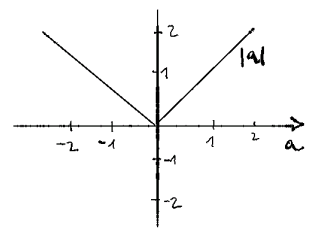
\includegraphics[width=0.4\textwidth]{betrag.png}
    \caption{Geschichte auf Linearer Zeitachse.}
    \label{fig:time_lin}
\end{figure}


\newpage
% \begin{landscape}
\begin{figure}[h!]
    \centering
    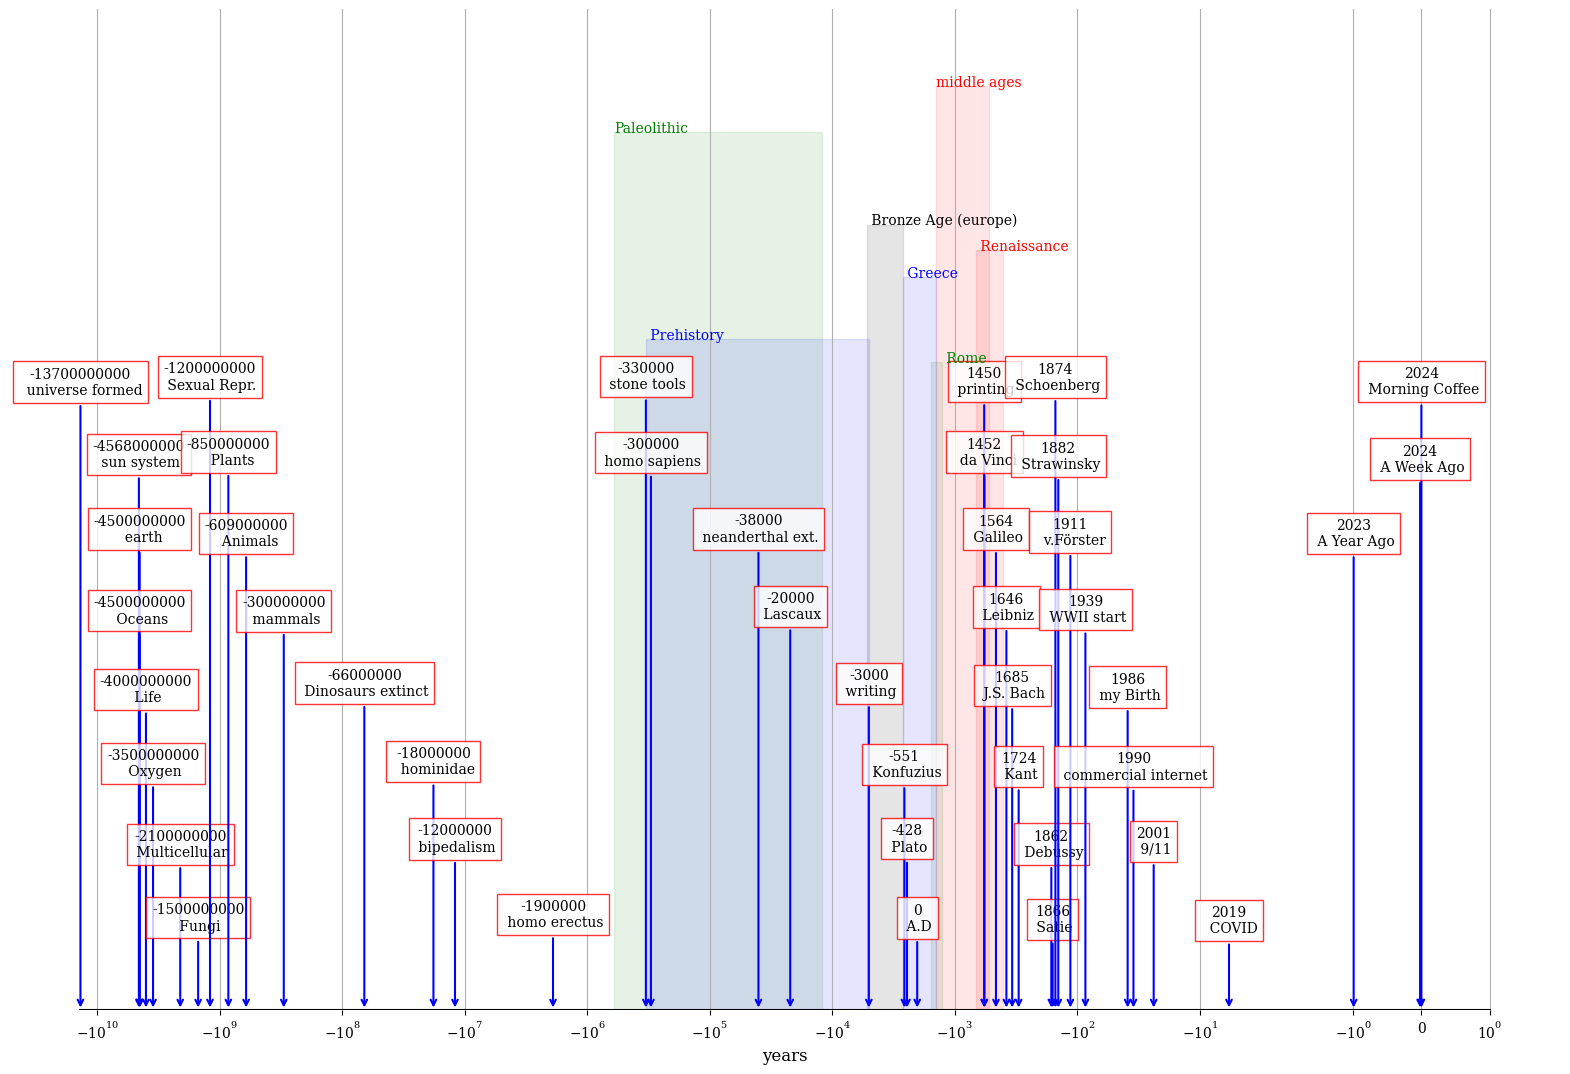
\includegraphics[height=\textwidth, angle=90]{img/time_log.png}
    \caption{Geschichte auf Logarithmischer Zeitachse.}
    \label{fig:time_log}
\end{figure}
% \end{landscape}





\section{Aufgaben und Beispiele}

\begin{enumerate}
    \item $\forall x \in \mathbb{R}, \exists y \in \mathbb{R} \text{ sodass } x + y = 0$. Was bedeutet dieser Ausdruck? Ist er wahr oder falsch?
    \item Gegeben sind die Mengen in Abb. \ref{fig:dreiMengen}. Zeichne ein Diagramm für:
    \begin{enumerate} % Use alphabetical labels for subitems
        \item $A \setminus (B \cup C)$
        \item $(A \cup B) \setminus C$
        \item $(B \cap C) \cup A$
    \end{enumerate}
    \item Zeichnen Sie einen Input/Output Plot für die Funktionen 
    \begin{enumerate} % Use alphabetical labels for subitems
        \item $f(x) = min(x, 0)$
        \item $f(x) = |x+1|-1$. Welche Bedeutung haben die beiden zahlen ($1$, $-1$ )? Wenn man sie verändern würde, was passiert mit dem Plot?
    \end{enumerate}
    \item Was gibt es zu Abb. \ref{fig:distortion_online} zu sagen?
    \item Konstruieren Sie (mache eine Formel, formale Beschreibung) einen 'hard clipper'. Dies ist eine Verzerrung. Die Verzerrung soll keine Werte 'durchlassen' die größer als 0.9 und kleiner als -0.9 sind. Zeichne den Graphen. Für Werte zwischen -0.9 und 0.9 soll sich der Verzerrer linear verhalten. Werden hier gerade oder ungerade Harmonische Erzeugt?
    \item Berechnen Sie die 'Spannung' $T$ (eine Kraft) in einer Piano Saite. Die Grundfrequenz der Saite ist 440 Hz, sie ist aus Stahl und ca. 50 cm lang. Gegeben ist folgende Formel: $f_0 = \frac{1}{\lambda} \sqrt{\frac{T}{\rho A}}$. Hier ist $\rho$ die Dichte des Materials und $A$ der Flächendurchschnitt der Saite. Wir nehmen an sie hat einen Durchmesser $d$ von ca. 1mm. Siehe Abb. \ref{fig:string_ex}.

    \item Beweisen Sie mittels Gleichungen \ref{eq:linearity1}, \ref{eq:linearity2} oder \ref{eq:linearity3} dass $f(x)=|x|$ nicht linear ist.



\end{enumerate}

\begin{figure}[h]
    \centering
    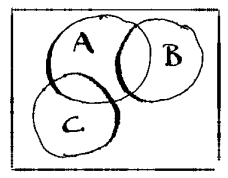
\includegraphics[width=0.3\textwidth]{img/dreiMeingen.png}
    \caption{Drei Mengen. }
    \label{fig:dreiMengen}
\end{figure}

\begin{figure}[h!]
    \centering
    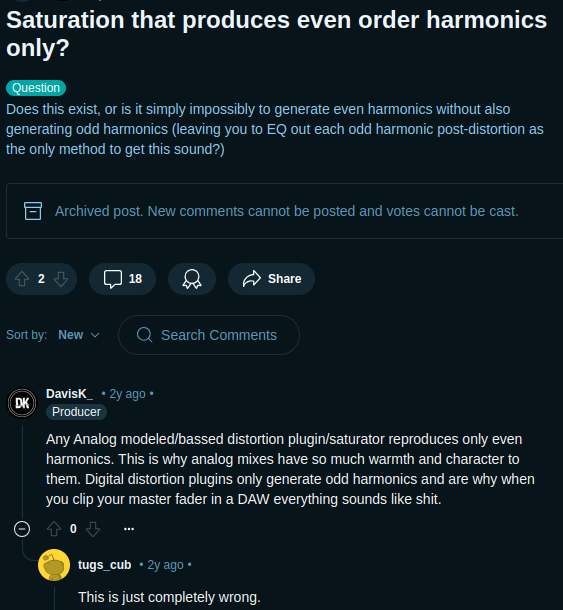
\includegraphics[ width= 0.7\textwidth]{img/reddit_distortion.png}
    \caption{Online Diskussionen über Verzerrung.}
    \label{fig:distortion_online}
\end{figure}

\begin{figure}[h!]
    \centering
    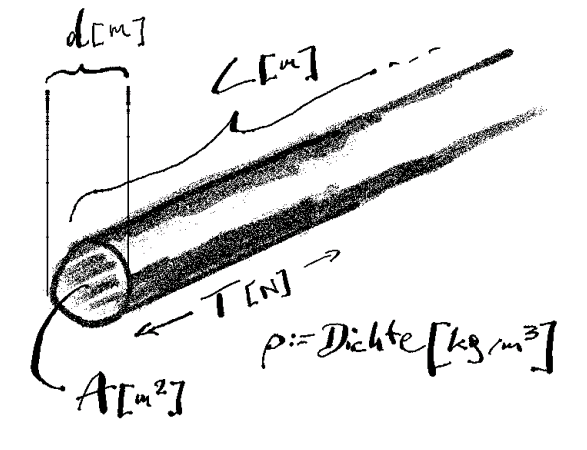
\includegraphics[ width= 0.4\textwidth]{img/saite_beispiel.png}
    \caption{Saite.}
    \label{fig:string_ex}
\end{figure}





%!TEX root = main.tex
\chapter{Wichtige Funktionen, Polynome, Python}

% \section{Wiederholung}

% \todo{Uebung: Ausdruck entwerfen der 2er Potenzen beschreibt.}

% \todo[]{Funktionsmanipulation im allgemeinen. }

\section{Funktionen Manipulieren}
Es ist wichtig ein Gefühl zu entwickeln wie sich einfache Rechenoperationen auf Funktionen auswirken und welche 'Audiointerpretation' hier naheliegt. Siehe Abbildung \ref{fig:functManipul}.
Hier eine Auflistung von Interpretationen unter der Annahme dass die horizontale Achse die Zeit $t$ darstellt:
\begin{itemize}
	\item $f(t) + a$: Gleichspannungsversatz hinzufügen/abziehen, Energie bei $0 Hz$, Verschieben der Welle nach 'oben und unten'
	\item $f(t+a)$: für $a<0$: \emph{Delay}, da Verschiebung auf der Zeitachse nach rechts. Besonders wichtig in der digital Technik, Filter etc. 
	\item $f(t) \cdot a$: Amplitudenänderung
	\item $f(t \cdot a)$: Zeitliche Streckung / Stauchung. Schnelleres oder langsameres abspielen, Änderung der Frequenz.

\end{itemize}

\begin{figure}[H]
	\centering
	%% Creator: Matplotlib, PGF backend
%%
%% To include the figure in your LaTeX document, write
%%   \input{<filename>.pgf}
%%
%% Make sure the required packages are loaded in your preamble
%%   \usepackage{pgf}
%%
%% Also ensure that all the required font packages are loaded; for instance,
%% the lmodern package is sometimes necessary when using math font.
%%   \usepackage{lmodern}
%%
%% Figures using additional raster images can only be included by \input if
%% they are in the same directory as the main LaTeX file. For loading figures
%% from other directories you can use the `import` package
%%   \usepackage{import}
%%
%% and then include the figures with
%%   \import{<path to file>}{<filename>.pgf}
%%
%% Matplotlib used the following preamble
%%   \def\mathdefault#1{#1}
%%   \everymath=\expandafter{\the\everymath\displaystyle}
%%   
%%   \usepackage{fontspec}
%%   \setmainfont{VeraSe.ttf}[Path=\detokenize{/usr/share/fonts/TTF/}]
%%   \setsansfont{DejaVuSans.ttf}[Path=\detokenize{/home/pl/miniconda3/lib/python3.12/site-packages/matplotlib/mpl-data/fonts/ttf/}]
%%   \setmonofont{DejaVuSansMono.ttf}[Path=\detokenize{/home/pl/miniconda3/lib/python3.12/site-packages/matplotlib/mpl-data/fonts/ttf/}]
%%   \makeatletter\@ifpackageloaded{underscore}{}{\usepackage[strings]{underscore}}\makeatother
%%
\begingroup%
\makeatletter%
\begin{pgfpicture}%
\pgfpathrectangle{\pgfpointorigin}{\pgfqpoint{5.254052in}{5.321247in}}%
\pgfusepath{use as bounding box, clip}%
\begin{pgfscope}%
\pgfsetbuttcap%
\pgfsetmiterjoin%
\definecolor{currentfill}{rgb}{1.000000,1.000000,1.000000}%
\pgfsetfillcolor{currentfill}%
\pgfsetlinewidth{0.000000pt}%
\definecolor{currentstroke}{rgb}{1.000000,1.000000,1.000000}%
\pgfsetstrokecolor{currentstroke}%
\pgfsetdash{}{0pt}%
\pgfpathmoveto{\pgfqpoint{0.000000in}{-0.000000in}}%
\pgfpathlineto{\pgfqpoint{5.254052in}{-0.000000in}}%
\pgfpathlineto{\pgfqpoint{5.254052in}{5.321247in}}%
\pgfpathlineto{\pgfqpoint{0.000000in}{5.321247in}}%
\pgfpathlineto{\pgfqpoint{0.000000in}{-0.000000in}}%
\pgfpathclose%
\pgfusepath{fill}%
\end{pgfscope}%
\begin{pgfscope}%
\pgfsetbuttcap%
\pgfsetmiterjoin%
\definecolor{currentfill}{rgb}{1.000000,1.000000,1.000000}%
\pgfsetfillcolor{currentfill}%
\pgfsetlinewidth{0.000000pt}%
\definecolor{currentstroke}{rgb}{0.000000,0.000000,0.000000}%
\pgfsetstrokecolor{currentstroke}%
\pgfsetstrokeopacity{0.000000}%
\pgfsetdash{}{0pt}%
\pgfpathmoveto{\pgfqpoint{0.393613in}{3.068486in}}%
\pgfpathlineto{\pgfqpoint{2.507249in}{3.068486in}}%
\pgfpathlineto{\pgfqpoint{2.507249in}{5.168486in}}%
\pgfpathlineto{\pgfqpoint{0.393613in}{5.168486in}}%
\pgfpathlineto{\pgfqpoint{0.393613in}{3.068486in}}%
\pgfpathclose%
\pgfusepath{fill}%
\end{pgfscope}%
\begin{pgfscope}%
\pgfsetbuttcap%
\pgfsetroundjoin%
\definecolor{currentfill}{rgb}{0.000000,0.000000,0.000000}%
\pgfsetfillcolor{currentfill}%
\pgfsetlinewidth{0.803000pt}%
\definecolor{currentstroke}{rgb}{0.000000,0.000000,0.000000}%
\pgfsetstrokecolor{currentstroke}%
\pgfsetdash{}{0pt}%
\pgfsys@defobject{currentmarker}{\pgfqpoint{0.000000in}{-0.048611in}}{\pgfqpoint{0.000000in}{0.000000in}}{%
\pgfpathmoveto{\pgfqpoint{0.000000in}{0.000000in}}%
\pgfpathlineto{\pgfqpoint{0.000000in}{-0.048611in}}%
\pgfusepath{stroke,fill}%
}%
\begin{pgfscope}%
\pgfsys@transformshift{0.393613in}{3.068486in}%
\pgfsys@useobject{currentmarker}{}%
\end{pgfscope}%
\end{pgfscope}%
\begin{pgfscope}%
\definecolor{textcolor}{rgb}{0.000000,0.000000,0.000000}%
\pgfsetstrokecolor{textcolor}%
\pgfsetfillcolor{textcolor}%
\pgftext[x=0.393613in,y=2.971264in,,top]{\color{textcolor}{\rmfamily\fontsize{10.000000}{12.000000}\selectfont\catcode`\^=\active\def^{\ifmmode\sp\else\^{}\fi}\catcode`\%=\active\def%{\%}\ensuremath{-}1.0}}%
\end{pgfscope}%
\begin{pgfscope}%
\pgfsetbuttcap%
\pgfsetroundjoin%
\definecolor{currentfill}{rgb}{0.000000,0.000000,0.000000}%
\pgfsetfillcolor{currentfill}%
\pgfsetlinewidth{0.803000pt}%
\definecolor{currentstroke}{rgb}{0.000000,0.000000,0.000000}%
\pgfsetstrokecolor{currentstroke}%
\pgfsetdash{}{0pt}%
\pgfsys@defobject{currentmarker}{\pgfqpoint{0.000000in}{-0.048611in}}{\pgfqpoint{0.000000in}{0.000000in}}{%
\pgfpathmoveto{\pgfqpoint{0.000000in}{0.000000in}}%
\pgfpathlineto{\pgfqpoint{0.000000in}{-0.048611in}}%
\pgfusepath{stroke,fill}%
}%
\begin{pgfscope}%
\pgfsys@transformshift{0.922022in}{3.068486in}%
\pgfsys@useobject{currentmarker}{}%
\end{pgfscope}%
\end{pgfscope}%
\begin{pgfscope}%
\definecolor{textcolor}{rgb}{0.000000,0.000000,0.000000}%
\pgfsetstrokecolor{textcolor}%
\pgfsetfillcolor{textcolor}%
\pgftext[x=0.922022in,y=2.971264in,,top]{\color{textcolor}{\rmfamily\fontsize{10.000000}{12.000000}\selectfont\catcode`\^=\active\def^{\ifmmode\sp\else\^{}\fi}\catcode`\%=\active\def%{\%}\ensuremath{-}0.5}}%
\end{pgfscope}%
\begin{pgfscope}%
\pgfsetbuttcap%
\pgfsetroundjoin%
\definecolor{currentfill}{rgb}{0.000000,0.000000,0.000000}%
\pgfsetfillcolor{currentfill}%
\pgfsetlinewidth{0.803000pt}%
\definecolor{currentstroke}{rgb}{0.000000,0.000000,0.000000}%
\pgfsetstrokecolor{currentstroke}%
\pgfsetdash{}{0pt}%
\pgfsys@defobject{currentmarker}{\pgfqpoint{0.000000in}{-0.048611in}}{\pgfqpoint{0.000000in}{0.000000in}}{%
\pgfpathmoveto{\pgfqpoint{0.000000in}{0.000000in}}%
\pgfpathlineto{\pgfqpoint{0.000000in}{-0.048611in}}%
\pgfusepath{stroke,fill}%
}%
\begin{pgfscope}%
\pgfsys@transformshift{1.450431in}{3.068486in}%
\pgfsys@useobject{currentmarker}{}%
\end{pgfscope}%
\end{pgfscope}%
\begin{pgfscope}%
\definecolor{textcolor}{rgb}{0.000000,0.000000,0.000000}%
\pgfsetstrokecolor{textcolor}%
\pgfsetfillcolor{textcolor}%
\pgftext[x=1.450431in,y=2.971264in,,top]{\color{textcolor}{\rmfamily\fontsize{10.000000}{12.000000}\selectfont\catcode`\^=\active\def^{\ifmmode\sp\else\^{}\fi}\catcode`\%=\active\def%{\%}0.0}}%
\end{pgfscope}%
\begin{pgfscope}%
\pgfsetbuttcap%
\pgfsetroundjoin%
\definecolor{currentfill}{rgb}{0.000000,0.000000,0.000000}%
\pgfsetfillcolor{currentfill}%
\pgfsetlinewidth{0.803000pt}%
\definecolor{currentstroke}{rgb}{0.000000,0.000000,0.000000}%
\pgfsetstrokecolor{currentstroke}%
\pgfsetdash{}{0pt}%
\pgfsys@defobject{currentmarker}{\pgfqpoint{0.000000in}{-0.048611in}}{\pgfqpoint{0.000000in}{0.000000in}}{%
\pgfpathmoveto{\pgfqpoint{0.000000in}{0.000000in}}%
\pgfpathlineto{\pgfqpoint{0.000000in}{-0.048611in}}%
\pgfusepath{stroke,fill}%
}%
\begin{pgfscope}%
\pgfsys@transformshift{1.978840in}{3.068486in}%
\pgfsys@useobject{currentmarker}{}%
\end{pgfscope}%
\end{pgfscope}%
\begin{pgfscope}%
\definecolor{textcolor}{rgb}{0.000000,0.000000,0.000000}%
\pgfsetstrokecolor{textcolor}%
\pgfsetfillcolor{textcolor}%
\pgftext[x=1.978840in,y=2.971264in,,top]{\color{textcolor}{\rmfamily\fontsize{10.000000}{12.000000}\selectfont\catcode`\^=\active\def^{\ifmmode\sp\else\^{}\fi}\catcode`\%=\active\def%{\%}0.5}}%
\end{pgfscope}%
\begin{pgfscope}%
\pgfsetbuttcap%
\pgfsetroundjoin%
\definecolor{currentfill}{rgb}{0.000000,0.000000,0.000000}%
\pgfsetfillcolor{currentfill}%
\pgfsetlinewidth{0.803000pt}%
\definecolor{currentstroke}{rgb}{0.000000,0.000000,0.000000}%
\pgfsetstrokecolor{currentstroke}%
\pgfsetdash{}{0pt}%
\pgfsys@defobject{currentmarker}{\pgfqpoint{0.000000in}{-0.048611in}}{\pgfqpoint{0.000000in}{0.000000in}}{%
\pgfpathmoveto{\pgfqpoint{0.000000in}{0.000000in}}%
\pgfpathlineto{\pgfqpoint{0.000000in}{-0.048611in}}%
\pgfusepath{stroke,fill}%
}%
\begin{pgfscope}%
\pgfsys@transformshift{2.507249in}{3.068486in}%
\pgfsys@useobject{currentmarker}{}%
\end{pgfscope}%
\end{pgfscope}%
\begin{pgfscope}%
\definecolor{textcolor}{rgb}{0.000000,0.000000,0.000000}%
\pgfsetstrokecolor{textcolor}%
\pgfsetfillcolor{textcolor}%
\pgftext[x=2.507249in,y=2.971264in,,top]{\color{textcolor}{\rmfamily\fontsize{10.000000}{12.000000}\selectfont\catcode`\^=\active\def^{\ifmmode\sp\else\^{}\fi}\catcode`\%=\active\def%{\%}1.0}}%
\end{pgfscope}%
\begin{pgfscope}%
\definecolor{textcolor}{rgb}{0.000000,0.000000,0.000000}%
\pgfsetstrokecolor{textcolor}%
\pgfsetfillcolor{textcolor}%
\pgftext[x=1.450431in,y=2.781295in,,top]{\color{textcolor}{\rmfamily\fontsize{12.000000}{14.400000}\selectfont\catcode`\^=\active\def^{\ifmmode\sp\else\^{}\fi}\catcode`\%=\active\def%{\%}$t$}}%
\end{pgfscope}%
\begin{pgfscope}%
\pgfsetbuttcap%
\pgfsetroundjoin%
\definecolor{currentfill}{rgb}{0.000000,0.000000,0.000000}%
\pgfsetfillcolor{currentfill}%
\pgfsetlinewidth{0.803000pt}%
\definecolor{currentstroke}{rgb}{0.000000,0.000000,0.000000}%
\pgfsetstrokecolor{currentstroke}%
\pgfsetdash{}{0pt}%
\pgfsys@defobject{currentmarker}{\pgfqpoint{-0.048611in}{0.000000in}}{\pgfqpoint{-0.000000in}{0.000000in}}{%
\pgfpathmoveto{\pgfqpoint{-0.000000in}{0.000000in}}%
\pgfpathlineto{\pgfqpoint{-0.048611in}{0.000000in}}%
\pgfusepath{stroke,fill}%
}%
\begin{pgfscope}%
\pgfsys@transformshift{0.393613in}{3.068486in}%
\pgfsys@useobject{currentmarker}{}%
\end{pgfscope}%
\end{pgfscope}%
\begin{pgfscope}%
\definecolor{textcolor}{rgb}{0.000000,0.000000,0.000000}%
\pgfsetstrokecolor{textcolor}%
\pgfsetfillcolor{textcolor}%
\pgftext[x=0.100000in, y=3.015724in, left, base]{\color{textcolor}{\rmfamily\fontsize{10.000000}{12.000000}\selectfont\catcode`\^=\active\def^{\ifmmode\sp\else\^{}\fi}\catcode`\%=\active\def%{\%}\ensuremath{-}2}}%
\end{pgfscope}%
\begin{pgfscope}%
\pgfsetbuttcap%
\pgfsetroundjoin%
\definecolor{currentfill}{rgb}{0.000000,0.000000,0.000000}%
\pgfsetfillcolor{currentfill}%
\pgfsetlinewidth{0.803000pt}%
\definecolor{currentstroke}{rgb}{0.000000,0.000000,0.000000}%
\pgfsetstrokecolor{currentstroke}%
\pgfsetdash{}{0pt}%
\pgfsys@defobject{currentmarker}{\pgfqpoint{-0.048611in}{0.000000in}}{\pgfqpoint{-0.000000in}{0.000000in}}{%
\pgfpathmoveto{\pgfqpoint{-0.000000in}{0.000000in}}%
\pgfpathlineto{\pgfqpoint{-0.048611in}{0.000000in}}%
\pgfusepath{stroke,fill}%
}%
\begin{pgfscope}%
\pgfsys@transformshift{0.393613in}{3.593486in}%
\pgfsys@useobject{currentmarker}{}%
\end{pgfscope}%
\end{pgfscope}%
\begin{pgfscope}%
\definecolor{textcolor}{rgb}{0.000000,0.000000,0.000000}%
\pgfsetstrokecolor{textcolor}%
\pgfsetfillcolor{textcolor}%
\pgftext[x=0.100000in, y=3.540724in, left, base]{\color{textcolor}{\rmfamily\fontsize{10.000000}{12.000000}\selectfont\catcode`\^=\active\def^{\ifmmode\sp\else\^{}\fi}\catcode`\%=\active\def%{\%}\ensuremath{-}1}}%
\end{pgfscope}%
\begin{pgfscope}%
\pgfsetbuttcap%
\pgfsetroundjoin%
\definecolor{currentfill}{rgb}{0.000000,0.000000,0.000000}%
\pgfsetfillcolor{currentfill}%
\pgfsetlinewidth{0.803000pt}%
\definecolor{currentstroke}{rgb}{0.000000,0.000000,0.000000}%
\pgfsetstrokecolor{currentstroke}%
\pgfsetdash{}{0pt}%
\pgfsys@defobject{currentmarker}{\pgfqpoint{-0.048611in}{0.000000in}}{\pgfqpoint{-0.000000in}{0.000000in}}{%
\pgfpathmoveto{\pgfqpoint{-0.000000in}{0.000000in}}%
\pgfpathlineto{\pgfqpoint{-0.048611in}{0.000000in}}%
\pgfusepath{stroke,fill}%
}%
\begin{pgfscope}%
\pgfsys@transformshift{0.393613in}{4.118486in}%
\pgfsys@useobject{currentmarker}{}%
\end{pgfscope}%
\end{pgfscope}%
\begin{pgfscope}%
\definecolor{textcolor}{rgb}{0.000000,0.000000,0.000000}%
\pgfsetstrokecolor{textcolor}%
\pgfsetfillcolor{textcolor}%
\pgftext[x=0.208025in, y=4.065724in, left, base]{\color{textcolor}{\rmfamily\fontsize{10.000000}{12.000000}\selectfont\catcode`\^=\active\def^{\ifmmode\sp\else\^{}\fi}\catcode`\%=\active\def%{\%}0}}%
\end{pgfscope}%
\begin{pgfscope}%
\pgfsetbuttcap%
\pgfsetroundjoin%
\definecolor{currentfill}{rgb}{0.000000,0.000000,0.000000}%
\pgfsetfillcolor{currentfill}%
\pgfsetlinewidth{0.803000pt}%
\definecolor{currentstroke}{rgb}{0.000000,0.000000,0.000000}%
\pgfsetstrokecolor{currentstroke}%
\pgfsetdash{}{0pt}%
\pgfsys@defobject{currentmarker}{\pgfqpoint{-0.048611in}{0.000000in}}{\pgfqpoint{-0.000000in}{0.000000in}}{%
\pgfpathmoveto{\pgfqpoint{-0.000000in}{0.000000in}}%
\pgfpathlineto{\pgfqpoint{-0.048611in}{0.000000in}}%
\pgfusepath{stroke,fill}%
}%
\begin{pgfscope}%
\pgfsys@transformshift{0.393613in}{4.643486in}%
\pgfsys@useobject{currentmarker}{}%
\end{pgfscope}%
\end{pgfscope}%
\begin{pgfscope}%
\definecolor{textcolor}{rgb}{0.000000,0.000000,0.000000}%
\pgfsetstrokecolor{textcolor}%
\pgfsetfillcolor{textcolor}%
\pgftext[x=0.208025in, y=4.590724in, left, base]{\color{textcolor}{\rmfamily\fontsize{10.000000}{12.000000}\selectfont\catcode`\^=\active\def^{\ifmmode\sp\else\^{}\fi}\catcode`\%=\active\def%{\%}1}}%
\end{pgfscope}%
\begin{pgfscope}%
\pgfsetbuttcap%
\pgfsetroundjoin%
\definecolor{currentfill}{rgb}{0.000000,0.000000,0.000000}%
\pgfsetfillcolor{currentfill}%
\pgfsetlinewidth{0.803000pt}%
\definecolor{currentstroke}{rgb}{0.000000,0.000000,0.000000}%
\pgfsetstrokecolor{currentstroke}%
\pgfsetdash{}{0pt}%
\pgfsys@defobject{currentmarker}{\pgfqpoint{-0.048611in}{0.000000in}}{\pgfqpoint{-0.000000in}{0.000000in}}{%
\pgfpathmoveto{\pgfqpoint{-0.000000in}{0.000000in}}%
\pgfpathlineto{\pgfqpoint{-0.048611in}{0.000000in}}%
\pgfusepath{stroke,fill}%
}%
\begin{pgfscope}%
\pgfsys@transformshift{0.393613in}{5.168486in}%
\pgfsys@useobject{currentmarker}{}%
\end{pgfscope}%
\end{pgfscope}%
\begin{pgfscope}%
\definecolor{textcolor}{rgb}{0.000000,0.000000,0.000000}%
\pgfsetstrokecolor{textcolor}%
\pgfsetfillcolor{textcolor}%
\pgftext[x=0.208025in, y=5.115724in, left, base]{\color{textcolor}{\rmfamily\fontsize{10.000000}{12.000000}\selectfont\catcode`\^=\active\def^{\ifmmode\sp\else\^{}\fi}\catcode`\%=\active\def%{\%}2}}%
\end{pgfscope}%
\begin{pgfscope}%
\pgfpathrectangle{\pgfqpoint{0.393613in}{3.068486in}}{\pgfqpoint{2.113636in}{2.100000in}}%
\pgfusepath{clip}%
\pgfsetbuttcap%
\pgfsetroundjoin%
\pgfsetlinewidth{0.501875pt}%
\definecolor{currentstroke}{rgb}{0.000000,0.000000,0.000000}%
\pgfsetstrokecolor{currentstroke}%
\pgfsetdash{{1.850000pt}{0.800000pt}}{0.000000pt}%
\pgfpathmoveto{\pgfqpoint{0.393613in}{4.118486in}}%
\pgfpathlineto{\pgfqpoint{2.507249in}{4.118486in}}%
\pgfusepath{stroke}%
\end{pgfscope}%
\begin{pgfscope}%
\pgfpathrectangle{\pgfqpoint{0.393613in}{3.068486in}}{\pgfqpoint{2.113636in}{2.100000in}}%
\pgfusepath{clip}%
\pgfsetbuttcap%
\pgfsetroundjoin%
\pgfsetlinewidth{0.501875pt}%
\definecolor{currentstroke}{rgb}{0.000000,0.000000,0.000000}%
\pgfsetstrokecolor{currentstroke}%
\pgfsetdash{{1.850000pt}{0.800000pt}}{0.000000pt}%
\pgfpathmoveto{\pgfqpoint{1.450431in}{3.068486in}}%
\pgfpathlineto{\pgfqpoint{1.450431in}{5.168486in}}%
\pgfusepath{stroke}%
\end{pgfscope}%
\begin{pgfscope}%
\pgfpathrectangle{\pgfqpoint{0.393613in}{3.068486in}}{\pgfqpoint{2.113636in}{2.100000in}}%
\pgfusepath{clip}%
\pgfsetrectcap%
\pgfsetroundjoin%
\pgfsetlinewidth{1.505625pt}%
\definecolor{currentstroke}{rgb}{0.000000,0.000000,0.000000}%
\pgfsetstrokecolor{currentstroke}%
\pgfsetdash{}{0pt}%
\pgfpathmoveto{\pgfqpoint{0.393613in}{3.952409in}}%
\pgfpathlineto{\pgfqpoint{0.438844in}{3.855579in}}%
\pgfpathlineto{\pgfqpoint{0.524235in}{3.672104in}}%
\pgfpathlineto{\pgfqpoint{0.558053in}{3.605241in}}%
\pgfpathlineto{\pgfqpoint{0.586376in}{3.554026in}}%
\pgfpathlineto{\pgfqpoint{0.610894in}{3.514098in}}%
\pgfpathlineto{\pgfqpoint{0.633299in}{3.481760in}}%
\pgfpathlineto{\pgfqpoint{0.653590in}{3.456269in}}%
\pgfpathlineto{\pgfqpoint{0.672190in}{3.436333in}}%
\pgfpathlineto{\pgfqpoint{0.689522in}{3.420888in}}%
\pgfpathlineto{\pgfqpoint{0.706008in}{3.409130in}}%
\pgfpathlineto{\pgfqpoint{0.721226in}{3.400906in}}%
\pgfpathlineto{\pgfqpoint{0.736022in}{3.395395in}}%
\pgfpathlineto{\pgfqpoint{0.750394in}{3.392434in}}%
\pgfpathlineto{\pgfqpoint{0.764344in}{3.391847in}}%
\pgfpathlineto{\pgfqpoint{0.778294in}{3.393533in}}%
\pgfpathlineto{\pgfqpoint{0.792244in}{3.397504in}}%
\pgfpathlineto{\pgfqpoint{0.806617in}{3.403985in}}%
\pgfpathlineto{\pgfqpoint{0.821413in}{3.413180in}}%
\pgfpathlineto{\pgfqpoint{0.836631in}{3.425283in}}%
\pgfpathlineto{\pgfqpoint{0.852694in}{3.440925in}}%
\pgfpathlineto{\pgfqpoint{0.870026in}{3.461035in}}%
\pgfpathlineto{\pgfqpoint{0.888203in}{3.485620in}}%
\pgfpathlineto{\pgfqpoint{0.907649in}{3.515725in}}%
\pgfpathlineto{\pgfqpoint{0.928785in}{3.552670in}}%
\pgfpathlineto{\pgfqpoint{0.951612in}{3.597165in}}%
\pgfpathlineto{\pgfqpoint{0.976976in}{3.651676in}}%
\pgfpathlineto{\pgfqpoint{1.005299in}{3.718049in}}%
\pgfpathlineto{\pgfqpoint{1.038272in}{3.801291in}}%
\pgfpathlineto{\pgfqpoint{1.079699in}{3.912339in}}%
\pgfpathlineto{\pgfqpoint{1.214972in}{4.279868in}}%
\pgfpathlineto{\pgfqpoint{1.247522in}{4.359104in}}%
\pgfpathlineto{\pgfqpoint{1.275422in}{4.421406in}}%
\pgfpathlineto{\pgfqpoint{1.300363in}{4.471896in}}%
\pgfpathlineto{\pgfqpoint{1.323190in}{4.513267in}}%
\pgfpathlineto{\pgfqpoint{1.344326in}{4.547086in}}%
\pgfpathlineto{\pgfqpoint{1.363772in}{4.574144in}}%
\pgfpathlineto{\pgfqpoint{1.381949in}{4.595758in}}%
\pgfpathlineto{\pgfqpoint{1.398858in}{4.612563in}}%
\pgfpathlineto{\pgfqpoint{1.414922in}{4.625511in}}%
\pgfpathlineto{\pgfqpoint{1.418303in}{4.627857in}}%
\pgfpathlineto{\pgfqpoint{1.419572in}{4.786202in}}%
\pgfpathlineto{\pgfqpoint{1.434790in}{4.794887in}}%
\pgfpathlineto{\pgfqpoint{1.449162in}{4.800599in}}%
\pgfpathlineto{\pgfqpoint{1.463113in}{4.803821in}}%
\pgfpathlineto{\pgfqpoint{1.477063in}{4.804762in}}%
\pgfpathlineto{\pgfqpoint{1.481712in}{4.804571in}}%
\pgfpathlineto{\pgfqpoint{1.482981in}{4.646975in}}%
\pgfpathlineto{\pgfqpoint{1.496931in}{4.644692in}}%
\pgfpathlineto{\pgfqpoint{1.511303in}{4.640007in}}%
\pgfpathlineto{\pgfqpoint{1.526099in}{4.632755in}}%
\pgfpathlineto{\pgfqpoint{1.541317in}{4.622783in}}%
\pgfpathlineto{\pgfqpoint{1.557381in}{4.609576in}}%
\pgfpathlineto{\pgfqpoint{1.574712in}{4.592357in}}%
\pgfpathlineto{\pgfqpoint{1.593312in}{4.570617in}}%
\pgfpathlineto{\pgfqpoint{1.613181in}{4.543899in}}%
\pgfpathlineto{\pgfqpoint{1.635162in}{4.510474in}}%
\pgfpathlineto{\pgfqpoint{1.659258in}{4.469669in}}%
\pgfpathlineto{\pgfqpoint{1.686735in}{4.418598in}}%
\pgfpathlineto{\pgfqpoint{1.719285in}{4.353166in}}%
\pgfpathlineto{\pgfqpoint{1.763249in}{4.259329in}}%
\pgfpathlineto{\pgfqpoint{1.854558in}{4.063266in}}%
\pgfpathlineto{\pgfqpoint{1.887953in}{3.997565in}}%
\pgfpathlineto{\pgfqpoint{1.915853in}{3.947401in}}%
\pgfpathlineto{\pgfqpoint{1.940372in}{3.907735in}}%
\pgfpathlineto{\pgfqpoint{1.962353in}{3.876233in}}%
\pgfpathlineto{\pgfqpoint{1.982644in}{3.850932in}}%
\pgfpathlineto{\pgfqpoint{2.001244in}{3.831182in}}%
\pgfpathlineto{\pgfqpoint{2.018576in}{3.815919in}}%
\pgfpathlineto{\pgfqpoint{2.034640in}{3.804602in}}%
\pgfpathlineto{\pgfqpoint{2.049858in}{3.796478in}}%
\pgfpathlineto{\pgfqpoint{2.064653in}{3.791066in}}%
\pgfpathlineto{\pgfqpoint{2.079026in}{3.788204in}}%
\pgfpathlineto{\pgfqpoint{2.092976in}{3.787713in}}%
\pgfpathlineto{\pgfqpoint{2.106926in}{3.789496in}}%
\pgfpathlineto{\pgfqpoint{2.120876in}{3.793565in}}%
\pgfpathlineto{\pgfqpoint{2.135249in}{3.800146in}}%
\pgfpathlineto{\pgfqpoint{2.150044in}{3.809443in}}%
\pgfpathlineto{\pgfqpoint{2.165263in}{3.821650in}}%
\pgfpathlineto{\pgfqpoint{2.181326in}{3.837401in}}%
\pgfpathlineto{\pgfqpoint{2.198658in}{3.857624in}}%
\pgfpathlineto{\pgfqpoint{2.216835in}{3.882325in}}%
\pgfpathlineto{\pgfqpoint{2.236281in}{3.912546in}}%
\pgfpathlineto{\pgfqpoint{2.257417in}{3.949611in}}%
\pgfpathlineto{\pgfqpoint{2.280244in}{3.994225in}}%
\pgfpathlineto{\pgfqpoint{2.305608in}{4.048854in}}%
\pgfpathlineto{\pgfqpoint{2.333931in}{4.115340in}}%
\pgfpathlineto{\pgfqpoint{2.366903in}{4.198683in}}%
\pgfpathlineto{\pgfqpoint{2.408753in}{4.310970in}}%
\pgfpathlineto{\pgfqpoint{2.507249in}{4.582409in}}%
\pgfpathlineto{\pgfqpoint{2.507249in}{4.582409in}}%
\pgfusepath{stroke}%
\end{pgfscope}%
\begin{pgfscope}%
\pgfpathrectangle{\pgfqpoint{0.393613in}{3.068486in}}{\pgfqpoint{2.113636in}{2.100000in}}%
\pgfusepath{clip}%
\pgfsetbuttcap%
\pgfsetroundjoin%
\pgfsetlinewidth{1.505625pt}%
\definecolor{currentstroke}{rgb}{0.000000,0.000000,0.000000}%
\pgfsetstrokecolor{currentstroke}%
\pgfsetdash{{5.550000pt}{2.400000pt}}{0.000000pt}%
\pgfpathmoveto{\pgfqpoint{0.393613in}{4.214909in}}%
\pgfpathlineto{\pgfqpoint{0.438844in}{4.118079in}}%
\pgfpathlineto{\pgfqpoint{0.524235in}{3.934604in}}%
\pgfpathlineto{\pgfqpoint{0.558053in}{3.867741in}}%
\pgfpathlineto{\pgfqpoint{0.586376in}{3.816526in}}%
\pgfpathlineto{\pgfqpoint{0.610894in}{3.776598in}}%
\pgfpathlineto{\pgfqpoint{0.633299in}{3.744260in}}%
\pgfpathlineto{\pgfqpoint{0.653590in}{3.718769in}}%
\pgfpathlineto{\pgfqpoint{0.672190in}{3.698833in}}%
\pgfpathlineto{\pgfqpoint{0.689522in}{3.683388in}}%
\pgfpathlineto{\pgfqpoint{0.706008in}{3.671630in}}%
\pgfpathlineto{\pgfqpoint{0.721226in}{3.663406in}}%
\pgfpathlineto{\pgfqpoint{0.736022in}{3.657895in}}%
\pgfpathlineto{\pgfqpoint{0.750394in}{3.654934in}}%
\pgfpathlineto{\pgfqpoint{0.764344in}{3.654347in}}%
\pgfpathlineto{\pgfqpoint{0.778294in}{3.656033in}}%
\pgfpathlineto{\pgfqpoint{0.792244in}{3.660004in}}%
\pgfpathlineto{\pgfqpoint{0.806617in}{3.666485in}}%
\pgfpathlineto{\pgfqpoint{0.821413in}{3.675680in}}%
\pgfpathlineto{\pgfqpoint{0.836631in}{3.687783in}}%
\pgfpathlineto{\pgfqpoint{0.852694in}{3.703425in}}%
\pgfpathlineto{\pgfqpoint{0.870026in}{3.723535in}}%
\pgfpathlineto{\pgfqpoint{0.888203in}{3.748120in}}%
\pgfpathlineto{\pgfqpoint{0.907649in}{3.778225in}}%
\pgfpathlineto{\pgfqpoint{0.928785in}{3.815170in}}%
\pgfpathlineto{\pgfqpoint{0.951612in}{3.859665in}}%
\pgfpathlineto{\pgfqpoint{0.976976in}{3.914176in}}%
\pgfpathlineto{\pgfqpoint{1.005299in}{3.980549in}}%
\pgfpathlineto{\pgfqpoint{1.038272in}{4.063791in}}%
\pgfpathlineto{\pgfqpoint{1.079699in}{4.174839in}}%
\pgfpathlineto{\pgfqpoint{1.214972in}{4.542368in}}%
\pgfpathlineto{\pgfqpoint{1.247522in}{4.621604in}}%
\pgfpathlineto{\pgfqpoint{1.275422in}{4.683906in}}%
\pgfpathlineto{\pgfqpoint{1.300363in}{4.734396in}}%
\pgfpathlineto{\pgfqpoint{1.323190in}{4.775767in}}%
\pgfpathlineto{\pgfqpoint{1.344326in}{4.809586in}}%
\pgfpathlineto{\pgfqpoint{1.363772in}{4.836644in}}%
\pgfpathlineto{\pgfqpoint{1.381949in}{4.858258in}}%
\pgfpathlineto{\pgfqpoint{1.398858in}{4.875063in}}%
\pgfpathlineto{\pgfqpoint{1.414922in}{4.888011in}}%
\pgfpathlineto{\pgfqpoint{1.418303in}{4.890357in}}%
\pgfpathlineto{\pgfqpoint{1.419572in}{5.048702in}}%
\pgfpathlineto{\pgfqpoint{1.434790in}{5.057387in}}%
\pgfpathlineto{\pgfqpoint{1.449162in}{5.063099in}}%
\pgfpathlineto{\pgfqpoint{1.463113in}{5.066321in}}%
\pgfpathlineto{\pgfqpoint{1.477063in}{5.067262in}}%
\pgfpathlineto{\pgfqpoint{1.481712in}{5.067071in}}%
\pgfpathlineto{\pgfqpoint{1.482981in}{4.909475in}}%
\pgfpathlineto{\pgfqpoint{1.496931in}{4.907192in}}%
\pgfpathlineto{\pgfqpoint{1.511303in}{4.902507in}}%
\pgfpathlineto{\pgfqpoint{1.526099in}{4.895255in}}%
\pgfpathlineto{\pgfqpoint{1.541317in}{4.885283in}}%
\pgfpathlineto{\pgfqpoint{1.557381in}{4.872076in}}%
\pgfpathlineto{\pgfqpoint{1.574712in}{4.854857in}}%
\pgfpathlineto{\pgfqpoint{1.593312in}{4.833117in}}%
\pgfpathlineto{\pgfqpoint{1.613181in}{4.806399in}}%
\pgfpathlineto{\pgfqpoint{1.635162in}{4.772974in}}%
\pgfpathlineto{\pgfqpoint{1.659258in}{4.732169in}}%
\pgfpathlineto{\pgfqpoint{1.686735in}{4.681098in}}%
\pgfpathlineto{\pgfqpoint{1.719285in}{4.615666in}}%
\pgfpathlineto{\pgfqpoint{1.763249in}{4.521829in}}%
\pgfpathlineto{\pgfqpoint{1.854558in}{4.325766in}}%
\pgfpathlineto{\pgfqpoint{1.887953in}{4.260065in}}%
\pgfpathlineto{\pgfqpoint{1.915853in}{4.209901in}}%
\pgfpathlineto{\pgfqpoint{1.940372in}{4.170235in}}%
\pgfpathlineto{\pgfqpoint{1.962353in}{4.138733in}}%
\pgfpathlineto{\pgfqpoint{1.982644in}{4.113432in}}%
\pgfpathlineto{\pgfqpoint{2.001244in}{4.093682in}}%
\pgfpathlineto{\pgfqpoint{2.018576in}{4.078419in}}%
\pgfpathlineto{\pgfqpoint{2.034640in}{4.067102in}}%
\pgfpathlineto{\pgfqpoint{2.049858in}{4.058978in}}%
\pgfpathlineto{\pgfqpoint{2.064653in}{4.053566in}}%
\pgfpathlineto{\pgfqpoint{2.079026in}{4.050704in}}%
\pgfpathlineto{\pgfqpoint{2.092976in}{4.050213in}}%
\pgfpathlineto{\pgfqpoint{2.106926in}{4.051996in}}%
\pgfpathlineto{\pgfqpoint{2.120876in}{4.056065in}}%
\pgfpathlineto{\pgfqpoint{2.135249in}{4.062646in}}%
\pgfpathlineto{\pgfqpoint{2.150044in}{4.071943in}}%
\pgfpathlineto{\pgfqpoint{2.165263in}{4.084150in}}%
\pgfpathlineto{\pgfqpoint{2.181326in}{4.099901in}}%
\pgfpathlineto{\pgfqpoint{2.198658in}{4.120124in}}%
\pgfpathlineto{\pgfqpoint{2.216835in}{4.144825in}}%
\pgfpathlineto{\pgfqpoint{2.236281in}{4.175046in}}%
\pgfpathlineto{\pgfqpoint{2.257417in}{4.212111in}}%
\pgfpathlineto{\pgfqpoint{2.280244in}{4.256725in}}%
\pgfpathlineto{\pgfqpoint{2.305608in}{4.311354in}}%
\pgfpathlineto{\pgfqpoint{2.333931in}{4.377840in}}%
\pgfpathlineto{\pgfqpoint{2.366903in}{4.461183in}}%
\pgfpathlineto{\pgfqpoint{2.408753in}{4.573470in}}%
\pgfpathlineto{\pgfqpoint{2.507249in}{4.844909in}}%
\pgfpathlineto{\pgfqpoint{2.507249in}{4.844909in}}%
\pgfusepath{stroke}%
\end{pgfscope}%
\begin{pgfscope}%
\pgfpathrectangle{\pgfqpoint{0.393613in}{3.068486in}}{\pgfqpoint{2.113636in}{2.100000in}}%
\pgfusepath{clip}%
\pgfsetbuttcap%
\pgfsetroundjoin%
\pgfsetlinewidth{1.505625pt}%
\definecolor{currentstroke}{rgb}{0.000000,0.000000,0.000000}%
\pgfsetstrokecolor{currentstroke}%
\pgfsetdash{{1.500000pt}{2.475000pt}}{0.000000pt}%
\pgfpathmoveto{\pgfqpoint{0.393613in}{3.689909in}}%
\pgfpathlineto{\pgfqpoint{0.438844in}{3.593079in}}%
\pgfpathlineto{\pgfqpoint{0.524235in}{3.409604in}}%
\pgfpathlineto{\pgfqpoint{0.558053in}{3.342741in}}%
\pgfpathlineto{\pgfqpoint{0.586376in}{3.291526in}}%
\pgfpathlineto{\pgfqpoint{0.610894in}{3.251598in}}%
\pgfpathlineto{\pgfqpoint{0.633299in}{3.219260in}}%
\pgfpathlineto{\pgfqpoint{0.653590in}{3.193769in}}%
\pgfpathlineto{\pgfqpoint{0.672190in}{3.173833in}}%
\pgfpathlineto{\pgfqpoint{0.689522in}{3.158388in}}%
\pgfpathlineto{\pgfqpoint{0.706008in}{3.146630in}}%
\pgfpathlineto{\pgfqpoint{0.721226in}{3.138406in}}%
\pgfpathlineto{\pgfqpoint{0.736022in}{3.132895in}}%
\pgfpathlineto{\pgfqpoint{0.750394in}{3.129934in}}%
\pgfpathlineto{\pgfqpoint{0.764344in}{3.129347in}}%
\pgfpathlineto{\pgfqpoint{0.778294in}{3.131033in}}%
\pgfpathlineto{\pgfqpoint{0.792244in}{3.135004in}}%
\pgfpathlineto{\pgfqpoint{0.806617in}{3.141485in}}%
\pgfpathlineto{\pgfqpoint{0.821413in}{3.150680in}}%
\pgfpathlineto{\pgfqpoint{0.836631in}{3.162783in}}%
\pgfpathlineto{\pgfqpoint{0.852694in}{3.178425in}}%
\pgfpathlineto{\pgfqpoint{0.870026in}{3.198535in}}%
\pgfpathlineto{\pgfqpoint{0.888203in}{3.223120in}}%
\pgfpathlineto{\pgfqpoint{0.907649in}{3.253225in}}%
\pgfpathlineto{\pgfqpoint{0.928785in}{3.290170in}}%
\pgfpathlineto{\pgfqpoint{0.951612in}{3.334665in}}%
\pgfpathlineto{\pgfqpoint{0.976976in}{3.389176in}}%
\pgfpathlineto{\pgfqpoint{1.005299in}{3.455549in}}%
\pgfpathlineto{\pgfqpoint{1.038272in}{3.538791in}}%
\pgfpathlineto{\pgfqpoint{1.079699in}{3.649839in}}%
\pgfpathlineto{\pgfqpoint{1.214972in}{4.017368in}}%
\pgfpathlineto{\pgfqpoint{1.247522in}{4.096604in}}%
\pgfpathlineto{\pgfqpoint{1.275422in}{4.158906in}}%
\pgfpathlineto{\pgfqpoint{1.300363in}{4.209396in}}%
\pgfpathlineto{\pgfqpoint{1.323190in}{4.250767in}}%
\pgfpathlineto{\pgfqpoint{1.344326in}{4.284586in}}%
\pgfpathlineto{\pgfqpoint{1.363772in}{4.311644in}}%
\pgfpathlineto{\pgfqpoint{1.381949in}{4.333258in}}%
\pgfpathlineto{\pgfqpoint{1.398858in}{4.350063in}}%
\pgfpathlineto{\pgfqpoint{1.414922in}{4.363011in}}%
\pgfpathlineto{\pgfqpoint{1.418303in}{4.365357in}}%
\pgfpathlineto{\pgfqpoint{1.419572in}{4.523702in}}%
\pgfpathlineto{\pgfqpoint{1.434790in}{4.532387in}}%
\pgfpathlineto{\pgfqpoint{1.449162in}{4.538099in}}%
\pgfpathlineto{\pgfqpoint{1.463113in}{4.541321in}}%
\pgfpathlineto{\pgfqpoint{1.477063in}{4.542262in}}%
\pgfpathlineto{\pgfqpoint{1.481712in}{4.542071in}}%
\pgfpathlineto{\pgfqpoint{1.482981in}{4.384475in}}%
\pgfpathlineto{\pgfqpoint{1.496931in}{4.382192in}}%
\pgfpathlineto{\pgfqpoint{1.511303in}{4.377507in}}%
\pgfpathlineto{\pgfqpoint{1.526099in}{4.370255in}}%
\pgfpathlineto{\pgfqpoint{1.541317in}{4.360283in}}%
\pgfpathlineto{\pgfqpoint{1.557381in}{4.347076in}}%
\pgfpathlineto{\pgfqpoint{1.574712in}{4.329857in}}%
\pgfpathlineto{\pgfqpoint{1.593312in}{4.308117in}}%
\pgfpathlineto{\pgfqpoint{1.613181in}{4.281399in}}%
\pgfpathlineto{\pgfqpoint{1.635162in}{4.247974in}}%
\pgfpathlineto{\pgfqpoint{1.659258in}{4.207169in}}%
\pgfpathlineto{\pgfqpoint{1.686735in}{4.156098in}}%
\pgfpathlineto{\pgfqpoint{1.719285in}{4.090666in}}%
\pgfpathlineto{\pgfqpoint{1.763249in}{3.996829in}}%
\pgfpathlineto{\pgfqpoint{1.854558in}{3.800766in}}%
\pgfpathlineto{\pgfqpoint{1.887953in}{3.735065in}}%
\pgfpathlineto{\pgfqpoint{1.915853in}{3.684901in}}%
\pgfpathlineto{\pgfqpoint{1.940372in}{3.645235in}}%
\pgfpathlineto{\pgfqpoint{1.962353in}{3.613733in}}%
\pgfpathlineto{\pgfqpoint{1.982644in}{3.588432in}}%
\pgfpathlineto{\pgfqpoint{2.001244in}{3.568682in}}%
\pgfpathlineto{\pgfqpoint{2.018576in}{3.553419in}}%
\pgfpathlineto{\pgfqpoint{2.034640in}{3.542102in}}%
\pgfpathlineto{\pgfqpoint{2.049858in}{3.533978in}}%
\pgfpathlineto{\pgfqpoint{2.064653in}{3.528566in}}%
\pgfpathlineto{\pgfqpoint{2.079026in}{3.525704in}}%
\pgfpathlineto{\pgfqpoint{2.092976in}{3.525213in}}%
\pgfpathlineto{\pgfqpoint{2.106926in}{3.526996in}}%
\pgfpathlineto{\pgfqpoint{2.120876in}{3.531065in}}%
\pgfpathlineto{\pgfqpoint{2.135249in}{3.537646in}}%
\pgfpathlineto{\pgfqpoint{2.150044in}{3.546943in}}%
\pgfpathlineto{\pgfqpoint{2.165263in}{3.559150in}}%
\pgfpathlineto{\pgfqpoint{2.181326in}{3.574901in}}%
\pgfpathlineto{\pgfqpoint{2.198658in}{3.595124in}}%
\pgfpathlineto{\pgfqpoint{2.216835in}{3.619825in}}%
\pgfpathlineto{\pgfqpoint{2.236281in}{3.650046in}}%
\pgfpathlineto{\pgfqpoint{2.257417in}{3.687111in}}%
\pgfpathlineto{\pgfqpoint{2.280244in}{3.731725in}}%
\pgfpathlineto{\pgfqpoint{2.305608in}{3.786354in}}%
\pgfpathlineto{\pgfqpoint{2.333931in}{3.852840in}}%
\pgfpathlineto{\pgfqpoint{2.366903in}{3.936183in}}%
\pgfpathlineto{\pgfqpoint{2.408753in}{4.048470in}}%
\pgfpathlineto{\pgfqpoint{2.507249in}{4.319909in}}%
\pgfpathlineto{\pgfqpoint{2.507249in}{4.319909in}}%
\pgfusepath{stroke}%
\end{pgfscope}%
\begin{pgfscope}%
\pgfsetbuttcap%
\pgfsetmiterjoin%
\definecolor{currentfill}{rgb}{1.000000,1.000000,1.000000}%
\pgfsetfillcolor{currentfill}%
\pgfsetfillopacity{0.800000}%
\pgfsetlinewidth{1.003750pt}%
\definecolor{currentstroke}{rgb}{0.800000,0.800000,0.800000}%
\pgfsetstrokecolor{currentstroke}%
\pgfsetstrokeopacity{0.800000}%
\pgfsetdash{}{0pt}%
\pgfpathmoveto{\pgfqpoint{0.934034in}{3.137930in}}%
\pgfpathlineto{\pgfqpoint{1.966827in}{3.137930in}}%
\pgfpathquadraticcurveto{\pgfqpoint{1.994605in}{3.137930in}}{\pgfqpoint{1.994605in}{3.165708in}}%
\pgfpathlineto{\pgfqpoint{1.994605in}{3.780888in}}%
\pgfpathquadraticcurveto{\pgfqpoint{1.994605in}{3.808666in}}{\pgfqpoint{1.966827in}{3.808666in}}%
\pgfpathlineto{\pgfqpoint{0.934034in}{3.808666in}}%
\pgfpathquadraticcurveto{\pgfqpoint{0.906256in}{3.808666in}}{\pgfqpoint{0.906256in}{3.780888in}}%
\pgfpathlineto{\pgfqpoint{0.906256in}{3.165708in}}%
\pgfpathquadraticcurveto{\pgfqpoint{0.906256in}{3.137930in}}{\pgfqpoint{0.934034in}{3.137930in}}%
\pgfpathlineto{\pgfqpoint{0.934034in}{3.137930in}}%
\pgfpathclose%
\pgfusepath{stroke,fill}%
\end{pgfscope}%
\begin{pgfscope}%
\pgfsetrectcap%
\pgfsetroundjoin%
\pgfsetlinewidth{1.505625pt}%
\definecolor{currentstroke}{rgb}{0.000000,0.000000,0.000000}%
\pgfsetstrokecolor{currentstroke}%
\pgfsetdash{}{0pt}%
\pgfpathmoveto{\pgfqpoint{0.961812in}{3.696199in}}%
\pgfpathlineto{\pgfqpoint{1.100701in}{3.696199in}}%
\pgfpathlineto{\pgfqpoint{1.239590in}{3.696199in}}%
\pgfusepath{stroke}%
\end{pgfscope}%
\begin{pgfscope}%
\definecolor{textcolor}{rgb}{0.000000,0.000000,0.000000}%
\pgfsetstrokecolor{textcolor}%
\pgfsetfillcolor{textcolor}%
\pgftext[x=1.350701in,y=3.647588in,left,base]{\color{textcolor}{\rmfamily\fontsize{10.000000}{12.000000}\selectfont\catcode`\^=\active\def^{\ifmmode\sp\else\^{}\fi}\catcode`\%=\active\def%{\%}$f(t)$}}%
\end{pgfscope}%
\begin{pgfscope}%
\pgfsetbuttcap%
\pgfsetroundjoin%
\pgfsetlinewidth{1.505625pt}%
\definecolor{currentstroke}{rgb}{0.000000,0.000000,0.000000}%
\pgfsetstrokecolor{currentstroke}%
\pgfsetdash{{5.550000pt}{2.400000pt}}{0.000000pt}%
\pgfpathmoveto{\pgfqpoint{0.961812in}{3.486509in}}%
\pgfpathlineto{\pgfqpoint{1.100701in}{3.486509in}}%
\pgfpathlineto{\pgfqpoint{1.239590in}{3.486509in}}%
\pgfusepath{stroke}%
\end{pgfscope}%
\begin{pgfscope}%
\definecolor{textcolor}{rgb}{0.000000,0.000000,0.000000}%
\pgfsetstrokecolor{textcolor}%
\pgfsetfillcolor{textcolor}%
\pgftext[x=1.350701in,y=3.437898in,left,base]{\color{textcolor}{\rmfamily\fontsize{10.000000}{12.000000}\selectfont\catcode`\^=\active\def^{\ifmmode\sp\else\^{}\fi}\catcode`\%=\active\def%{\%}$f(t)+0.5$}}%
\end{pgfscope}%
\begin{pgfscope}%
\pgfsetbuttcap%
\pgfsetroundjoin%
\pgfsetlinewidth{1.505625pt}%
\definecolor{currentstroke}{rgb}{0.000000,0.000000,0.000000}%
\pgfsetstrokecolor{currentstroke}%
\pgfsetdash{{1.500000pt}{2.475000pt}}{0.000000pt}%
\pgfpathmoveto{\pgfqpoint{0.961812in}{3.276819in}}%
\pgfpathlineto{\pgfqpoint{1.100701in}{3.276819in}}%
\pgfpathlineto{\pgfqpoint{1.239590in}{3.276819in}}%
\pgfusepath{stroke}%
\end{pgfscope}%
\begin{pgfscope}%
\definecolor{textcolor}{rgb}{0.000000,0.000000,0.000000}%
\pgfsetstrokecolor{textcolor}%
\pgfsetfillcolor{textcolor}%
\pgftext[x=1.350701in,y=3.228208in,left,base]{\color{textcolor}{\rmfamily\fontsize{10.000000}{12.000000}\selectfont\catcode`\^=\active\def^{\ifmmode\sp\else\^{}\fi}\catcode`\%=\active\def%{\%}$f(t)-0.5$}}%
\end{pgfscope}%
\begin{pgfscope}%
\pgfsetbuttcap%
\pgfsetmiterjoin%
\definecolor{currentfill}{rgb}{1.000000,1.000000,1.000000}%
\pgfsetfillcolor{currentfill}%
\pgfsetlinewidth{0.000000pt}%
\definecolor{currentstroke}{rgb}{0.000000,0.000000,0.000000}%
\pgfsetstrokecolor{currentstroke}%
\pgfsetstrokeopacity{0.000000}%
\pgfsetdash{}{0pt}%
\pgfpathmoveto{\pgfqpoint{2.929976in}{3.068486in}}%
\pgfpathlineto{\pgfqpoint{5.043613in}{3.068486in}}%
\pgfpathlineto{\pgfqpoint{5.043613in}{5.168486in}}%
\pgfpathlineto{\pgfqpoint{2.929976in}{5.168486in}}%
\pgfpathlineto{\pgfqpoint{2.929976in}{3.068486in}}%
\pgfpathclose%
\pgfusepath{fill}%
\end{pgfscope}%
\begin{pgfscope}%
\pgfsetbuttcap%
\pgfsetroundjoin%
\definecolor{currentfill}{rgb}{0.000000,0.000000,0.000000}%
\pgfsetfillcolor{currentfill}%
\pgfsetlinewidth{0.803000pt}%
\definecolor{currentstroke}{rgb}{0.000000,0.000000,0.000000}%
\pgfsetstrokecolor{currentstroke}%
\pgfsetdash{}{0pt}%
\pgfsys@defobject{currentmarker}{\pgfqpoint{0.000000in}{-0.048611in}}{\pgfqpoint{0.000000in}{0.000000in}}{%
\pgfpathmoveto{\pgfqpoint{0.000000in}{0.000000in}}%
\pgfpathlineto{\pgfqpoint{0.000000in}{-0.048611in}}%
\pgfusepath{stroke,fill}%
}%
\begin{pgfscope}%
\pgfsys@transformshift{2.929976in}{3.068486in}%
\pgfsys@useobject{currentmarker}{}%
\end{pgfscope}%
\end{pgfscope}%
\begin{pgfscope}%
\definecolor{textcolor}{rgb}{0.000000,0.000000,0.000000}%
\pgfsetstrokecolor{textcolor}%
\pgfsetfillcolor{textcolor}%
\pgftext[x=2.929976in,y=2.971264in,,top]{\color{textcolor}{\rmfamily\fontsize{10.000000}{12.000000}\selectfont\catcode`\^=\active\def^{\ifmmode\sp\else\^{}\fi}\catcode`\%=\active\def%{\%}\ensuremath{-}1.0}}%
\end{pgfscope}%
\begin{pgfscope}%
\pgfsetbuttcap%
\pgfsetroundjoin%
\definecolor{currentfill}{rgb}{0.000000,0.000000,0.000000}%
\pgfsetfillcolor{currentfill}%
\pgfsetlinewidth{0.803000pt}%
\definecolor{currentstroke}{rgb}{0.000000,0.000000,0.000000}%
\pgfsetstrokecolor{currentstroke}%
\pgfsetdash{}{0pt}%
\pgfsys@defobject{currentmarker}{\pgfqpoint{0.000000in}{-0.048611in}}{\pgfqpoint{0.000000in}{0.000000in}}{%
\pgfpathmoveto{\pgfqpoint{0.000000in}{0.000000in}}%
\pgfpathlineto{\pgfqpoint{0.000000in}{-0.048611in}}%
\pgfusepath{stroke,fill}%
}%
\begin{pgfscope}%
\pgfsys@transformshift{3.458385in}{3.068486in}%
\pgfsys@useobject{currentmarker}{}%
\end{pgfscope}%
\end{pgfscope}%
\begin{pgfscope}%
\definecolor{textcolor}{rgb}{0.000000,0.000000,0.000000}%
\pgfsetstrokecolor{textcolor}%
\pgfsetfillcolor{textcolor}%
\pgftext[x=3.458385in,y=2.971264in,,top]{\color{textcolor}{\rmfamily\fontsize{10.000000}{12.000000}\selectfont\catcode`\^=\active\def^{\ifmmode\sp\else\^{}\fi}\catcode`\%=\active\def%{\%}\ensuremath{-}0.5}}%
\end{pgfscope}%
\begin{pgfscope}%
\pgfsetbuttcap%
\pgfsetroundjoin%
\definecolor{currentfill}{rgb}{0.000000,0.000000,0.000000}%
\pgfsetfillcolor{currentfill}%
\pgfsetlinewidth{0.803000pt}%
\definecolor{currentstroke}{rgb}{0.000000,0.000000,0.000000}%
\pgfsetstrokecolor{currentstroke}%
\pgfsetdash{}{0pt}%
\pgfsys@defobject{currentmarker}{\pgfqpoint{0.000000in}{-0.048611in}}{\pgfqpoint{0.000000in}{0.000000in}}{%
\pgfpathmoveto{\pgfqpoint{0.000000in}{0.000000in}}%
\pgfpathlineto{\pgfqpoint{0.000000in}{-0.048611in}}%
\pgfusepath{stroke,fill}%
}%
\begin{pgfscope}%
\pgfsys@transformshift{3.986794in}{3.068486in}%
\pgfsys@useobject{currentmarker}{}%
\end{pgfscope}%
\end{pgfscope}%
\begin{pgfscope}%
\definecolor{textcolor}{rgb}{0.000000,0.000000,0.000000}%
\pgfsetstrokecolor{textcolor}%
\pgfsetfillcolor{textcolor}%
\pgftext[x=3.986794in,y=2.971264in,,top]{\color{textcolor}{\rmfamily\fontsize{10.000000}{12.000000}\selectfont\catcode`\^=\active\def^{\ifmmode\sp\else\^{}\fi}\catcode`\%=\active\def%{\%}0.0}}%
\end{pgfscope}%
\begin{pgfscope}%
\pgfsetbuttcap%
\pgfsetroundjoin%
\definecolor{currentfill}{rgb}{0.000000,0.000000,0.000000}%
\pgfsetfillcolor{currentfill}%
\pgfsetlinewidth{0.803000pt}%
\definecolor{currentstroke}{rgb}{0.000000,0.000000,0.000000}%
\pgfsetstrokecolor{currentstroke}%
\pgfsetdash{}{0pt}%
\pgfsys@defobject{currentmarker}{\pgfqpoint{0.000000in}{-0.048611in}}{\pgfqpoint{0.000000in}{0.000000in}}{%
\pgfpathmoveto{\pgfqpoint{0.000000in}{0.000000in}}%
\pgfpathlineto{\pgfqpoint{0.000000in}{-0.048611in}}%
\pgfusepath{stroke,fill}%
}%
\begin{pgfscope}%
\pgfsys@transformshift{4.515203in}{3.068486in}%
\pgfsys@useobject{currentmarker}{}%
\end{pgfscope}%
\end{pgfscope}%
\begin{pgfscope}%
\definecolor{textcolor}{rgb}{0.000000,0.000000,0.000000}%
\pgfsetstrokecolor{textcolor}%
\pgfsetfillcolor{textcolor}%
\pgftext[x=4.515203in,y=2.971264in,,top]{\color{textcolor}{\rmfamily\fontsize{10.000000}{12.000000}\selectfont\catcode`\^=\active\def^{\ifmmode\sp\else\^{}\fi}\catcode`\%=\active\def%{\%}0.5}}%
\end{pgfscope}%
\begin{pgfscope}%
\pgfsetbuttcap%
\pgfsetroundjoin%
\definecolor{currentfill}{rgb}{0.000000,0.000000,0.000000}%
\pgfsetfillcolor{currentfill}%
\pgfsetlinewidth{0.803000pt}%
\definecolor{currentstroke}{rgb}{0.000000,0.000000,0.000000}%
\pgfsetstrokecolor{currentstroke}%
\pgfsetdash{}{0pt}%
\pgfsys@defobject{currentmarker}{\pgfqpoint{0.000000in}{-0.048611in}}{\pgfqpoint{0.000000in}{0.000000in}}{%
\pgfpathmoveto{\pgfqpoint{0.000000in}{0.000000in}}%
\pgfpathlineto{\pgfqpoint{0.000000in}{-0.048611in}}%
\pgfusepath{stroke,fill}%
}%
\begin{pgfscope}%
\pgfsys@transformshift{5.043613in}{3.068486in}%
\pgfsys@useobject{currentmarker}{}%
\end{pgfscope}%
\end{pgfscope}%
\begin{pgfscope}%
\definecolor{textcolor}{rgb}{0.000000,0.000000,0.000000}%
\pgfsetstrokecolor{textcolor}%
\pgfsetfillcolor{textcolor}%
\pgftext[x=5.043613in,y=2.971264in,,top]{\color{textcolor}{\rmfamily\fontsize{10.000000}{12.000000}\selectfont\catcode`\^=\active\def^{\ifmmode\sp\else\^{}\fi}\catcode`\%=\active\def%{\%}1.0}}%
\end{pgfscope}%
\begin{pgfscope}%
\definecolor{textcolor}{rgb}{0.000000,0.000000,0.000000}%
\pgfsetstrokecolor{textcolor}%
\pgfsetfillcolor{textcolor}%
\pgftext[x=3.986794in,y=2.781295in,,top]{\color{textcolor}{\rmfamily\fontsize{12.000000}{14.400000}\selectfont\catcode`\^=\active\def^{\ifmmode\sp\else\^{}\fi}\catcode`\%=\active\def%{\%}$t$}}%
\end{pgfscope}%
\begin{pgfscope}%
\pgfsetbuttcap%
\pgfsetroundjoin%
\definecolor{currentfill}{rgb}{0.000000,0.000000,0.000000}%
\pgfsetfillcolor{currentfill}%
\pgfsetlinewidth{0.803000pt}%
\definecolor{currentstroke}{rgb}{0.000000,0.000000,0.000000}%
\pgfsetstrokecolor{currentstroke}%
\pgfsetdash{}{0pt}%
\pgfsys@defobject{currentmarker}{\pgfqpoint{-0.048611in}{0.000000in}}{\pgfqpoint{-0.000000in}{0.000000in}}{%
\pgfpathmoveto{\pgfqpoint{-0.000000in}{0.000000in}}%
\pgfpathlineto{\pgfqpoint{-0.048611in}{0.000000in}}%
\pgfusepath{stroke,fill}%
}%
\begin{pgfscope}%
\pgfsys@transformshift{2.929976in}{3.068486in}%
\pgfsys@useobject{currentmarker}{}%
\end{pgfscope}%
\end{pgfscope}%
\begin{pgfscope}%
\definecolor{textcolor}{rgb}{0.000000,0.000000,0.000000}%
\pgfsetstrokecolor{textcolor}%
\pgfsetfillcolor{textcolor}%
\pgftext[x=2.636364in, y=3.015724in, left, base]{\color{textcolor}{\rmfamily\fontsize{10.000000}{12.000000}\selectfont\catcode`\^=\active\def^{\ifmmode\sp\else\^{}\fi}\catcode`\%=\active\def%{\%}\ensuremath{-}2}}%
\end{pgfscope}%
\begin{pgfscope}%
\pgfsetbuttcap%
\pgfsetroundjoin%
\definecolor{currentfill}{rgb}{0.000000,0.000000,0.000000}%
\pgfsetfillcolor{currentfill}%
\pgfsetlinewidth{0.803000pt}%
\definecolor{currentstroke}{rgb}{0.000000,0.000000,0.000000}%
\pgfsetstrokecolor{currentstroke}%
\pgfsetdash{}{0pt}%
\pgfsys@defobject{currentmarker}{\pgfqpoint{-0.048611in}{0.000000in}}{\pgfqpoint{-0.000000in}{0.000000in}}{%
\pgfpathmoveto{\pgfqpoint{-0.000000in}{0.000000in}}%
\pgfpathlineto{\pgfqpoint{-0.048611in}{0.000000in}}%
\pgfusepath{stroke,fill}%
}%
\begin{pgfscope}%
\pgfsys@transformshift{2.929976in}{3.593486in}%
\pgfsys@useobject{currentmarker}{}%
\end{pgfscope}%
\end{pgfscope}%
\begin{pgfscope}%
\definecolor{textcolor}{rgb}{0.000000,0.000000,0.000000}%
\pgfsetstrokecolor{textcolor}%
\pgfsetfillcolor{textcolor}%
\pgftext[x=2.636364in, y=3.540724in, left, base]{\color{textcolor}{\rmfamily\fontsize{10.000000}{12.000000}\selectfont\catcode`\^=\active\def^{\ifmmode\sp\else\^{}\fi}\catcode`\%=\active\def%{\%}\ensuremath{-}1}}%
\end{pgfscope}%
\begin{pgfscope}%
\pgfsetbuttcap%
\pgfsetroundjoin%
\definecolor{currentfill}{rgb}{0.000000,0.000000,0.000000}%
\pgfsetfillcolor{currentfill}%
\pgfsetlinewidth{0.803000pt}%
\definecolor{currentstroke}{rgb}{0.000000,0.000000,0.000000}%
\pgfsetstrokecolor{currentstroke}%
\pgfsetdash{}{0pt}%
\pgfsys@defobject{currentmarker}{\pgfqpoint{-0.048611in}{0.000000in}}{\pgfqpoint{-0.000000in}{0.000000in}}{%
\pgfpathmoveto{\pgfqpoint{-0.000000in}{0.000000in}}%
\pgfpathlineto{\pgfqpoint{-0.048611in}{0.000000in}}%
\pgfusepath{stroke,fill}%
}%
\begin{pgfscope}%
\pgfsys@transformshift{2.929976in}{4.118486in}%
\pgfsys@useobject{currentmarker}{}%
\end{pgfscope}%
\end{pgfscope}%
\begin{pgfscope}%
\definecolor{textcolor}{rgb}{0.000000,0.000000,0.000000}%
\pgfsetstrokecolor{textcolor}%
\pgfsetfillcolor{textcolor}%
\pgftext[x=2.744389in, y=4.065724in, left, base]{\color{textcolor}{\rmfamily\fontsize{10.000000}{12.000000}\selectfont\catcode`\^=\active\def^{\ifmmode\sp\else\^{}\fi}\catcode`\%=\active\def%{\%}0}}%
\end{pgfscope}%
\begin{pgfscope}%
\pgfsetbuttcap%
\pgfsetroundjoin%
\definecolor{currentfill}{rgb}{0.000000,0.000000,0.000000}%
\pgfsetfillcolor{currentfill}%
\pgfsetlinewidth{0.803000pt}%
\definecolor{currentstroke}{rgb}{0.000000,0.000000,0.000000}%
\pgfsetstrokecolor{currentstroke}%
\pgfsetdash{}{0pt}%
\pgfsys@defobject{currentmarker}{\pgfqpoint{-0.048611in}{0.000000in}}{\pgfqpoint{-0.000000in}{0.000000in}}{%
\pgfpathmoveto{\pgfqpoint{-0.000000in}{0.000000in}}%
\pgfpathlineto{\pgfqpoint{-0.048611in}{0.000000in}}%
\pgfusepath{stroke,fill}%
}%
\begin{pgfscope}%
\pgfsys@transformshift{2.929976in}{4.643486in}%
\pgfsys@useobject{currentmarker}{}%
\end{pgfscope}%
\end{pgfscope}%
\begin{pgfscope}%
\definecolor{textcolor}{rgb}{0.000000,0.000000,0.000000}%
\pgfsetstrokecolor{textcolor}%
\pgfsetfillcolor{textcolor}%
\pgftext[x=2.744389in, y=4.590724in, left, base]{\color{textcolor}{\rmfamily\fontsize{10.000000}{12.000000}\selectfont\catcode`\^=\active\def^{\ifmmode\sp\else\^{}\fi}\catcode`\%=\active\def%{\%}1}}%
\end{pgfscope}%
\begin{pgfscope}%
\pgfsetbuttcap%
\pgfsetroundjoin%
\definecolor{currentfill}{rgb}{0.000000,0.000000,0.000000}%
\pgfsetfillcolor{currentfill}%
\pgfsetlinewidth{0.803000pt}%
\definecolor{currentstroke}{rgb}{0.000000,0.000000,0.000000}%
\pgfsetstrokecolor{currentstroke}%
\pgfsetdash{}{0pt}%
\pgfsys@defobject{currentmarker}{\pgfqpoint{-0.048611in}{0.000000in}}{\pgfqpoint{-0.000000in}{0.000000in}}{%
\pgfpathmoveto{\pgfqpoint{-0.000000in}{0.000000in}}%
\pgfpathlineto{\pgfqpoint{-0.048611in}{0.000000in}}%
\pgfusepath{stroke,fill}%
}%
\begin{pgfscope}%
\pgfsys@transformshift{2.929976in}{5.168486in}%
\pgfsys@useobject{currentmarker}{}%
\end{pgfscope}%
\end{pgfscope}%
\begin{pgfscope}%
\definecolor{textcolor}{rgb}{0.000000,0.000000,0.000000}%
\pgfsetstrokecolor{textcolor}%
\pgfsetfillcolor{textcolor}%
\pgftext[x=2.744389in, y=5.115724in, left, base]{\color{textcolor}{\rmfamily\fontsize{10.000000}{12.000000}\selectfont\catcode`\^=\active\def^{\ifmmode\sp\else\^{}\fi}\catcode`\%=\active\def%{\%}2}}%
\end{pgfscope}%
\begin{pgfscope}%
\pgfpathrectangle{\pgfqpoint{2.929976in}{3.068486in}}{\pgfqpoint{2.113636in}{2.100000in}}%
\pgfusepath{clip}%
\pgfsetbuttcap%
\pgfsetroundjoin%
\pgfsetlinewidth{0.501875pt}%
\definecolor{currentstroke}{rgb}{0.000000,0.000000,0.000000}%
\pgfsetstrokecolor{currentstroke}%
\pgfsetdash{{1.850000pt}{0.800000pt}}{0.000000pt}%
\pgfpathmoveto{\pgfqpoint{2.929976in}{4.118486in}}%
\pgfpathlineto{\pgfqpoint{5.043613in}{4.118486in}}%
\pgfusepath{stroke}%
\end{pgfscope}%
\begin{pgfscope}%
\pgfpathrectangle{\pgfqpoint{2.929976in}{3.068486in}}{\pgfqpoint{2.113636in}{2.100000in}}%
\pgfusepath{clip}%
\pgfsetbuttcap%
\pgfsetroundjoin%
\pgfsetlinewidth{0.501875pt}%
\definecolor{currentstroke}{rgb}{0.000000,0.000000,0.000000}%
\pgfsetstrokecolor{currentstroke}%
\pgfsetdash{{1.850000pt}{0.800000pt}}{0.000000pt}%
\pgfpathmoveto{\pgfqpoint{3.986794in}{3.068486in}}%
\pgfpathlineto{\pgfqpoint{3.986794in}{5.168486in}}%
\pgfusepath{stroke}%
\end{pgfscope}%
\begin{pgfscope}%
\pgfpathrectangle{\pgfqpoint{2.929976in}{3.068486in}}{\pgfqpoint{2.113636in}{2.100000in}}%
\pgfusepath{clip}%
\pgfsetrectcap%
\pgfsetroundjoin%
\pgfsetlinewidth{1.505625pt}%
\definecolor{currentstroke}{rgb}{0.000000,0.000000,0.000000}%
\pgfsetstrokecolor{currentstroke}%
\pgfsetdash{}{0pt}%
\pgfpathmoveto{\pgfqpoint{2.929976in}{3.952409in}}%
\pgfpathlineto{\pgfqpoint{2.975208in}{3.855579in}}%
\pgfpathlineto{\pgfqpoint{3.060599in}{3.672104in}}%
\pgfpathlineto{\pgfqpoint{3.094417in}{3.605241in}}%
\pgfpathlineto{\pgfqpoint{3.122740in}{3.554026in}}%
\pgfpathlineto{\pgfqpoint{3.147258in}{3.514098in}}%
\pgfpathlineto{\pgfqpoint{3.169662in}{3.481760in}}%
\pgfpathlineto{\pgfqpoint{3.189953in}{3.456269in}}%
\pgfpathlineto{\pgfqpoint{3.208553in}{3.436333in}}%
\pgfpathlineto{\pgfqpoint{3.225885in}{3.420888in}}%
\pgfpathlineto{\pgfqpoint{3.242372in}{3.409130in}}%
\pgfpathlineto{\pgfqpoint{3.257590in}{3.400906in}}%
\pgfpathlineto{\pgfqpoint{3.272385in}{3.395395in}}%
\pgfpathlineto{\pgfqpoint{3.286758in}{3.392434in}}%
\pgfpathlineto{\pgfqpoint{3.300708in}{3.391847in}}%
\pgfpathlineto{\pgfqpoint{3.314658in}{3.393533in}}%
\pgfpathlineto{\pgfqpoint{3.328608in}{3.397504in}}%
\pgfpathlineto{\pgfqpoint{3.342981in}{3.403985in}}%
\pgfpathlineto{\pgfqpoint{3.357776in}{3.413180in}}%
\pgfpathlineto{\pgfqpoint{3.372994in}{3.425283in}}%
\pgfpathlineto{\pgfqpoint{3.389058in}{3.440925in}}%
\pgfpathlineto{\pgfqpoint{3.406390in}{3.461035in}}%
\pgfpathlineto{\pgfqpoint{3.424567in}{3.485620in}}%
\pgfpathlineto{\pgfqpoint{3.444012in}{3.515725in}}%
\pgfpathlineto{\pgfqpoint{3.465149in}{3.552670in}}%
\pgfpathlineto{\pgfqpoint{3.487976in}{3.597165in}}%
\pgfpathlineto{\pgfqpoint{3.513340in}{3.651676in}}%
\pgfpathlineto{\pgfqpoint{3.541663in}{3.718049in}}%
\pgfpathlineto{\pgfqpoint{3.574635in}{3.801291in}}%
\pgfpathlineto{\pgfqpoint{3.616062in}{3.912339in}}%
\pgfpathlineto{\pgfqpoint{3.751335in}{4.279868in}}%
\pgfpathlineto{\pgfqpoint{3.783885in}{4.359104in}}%
\pgfpathlineto{\pgfqpoint{3.811785in}{4.421406in}}%
\pgfpathlineto{\pgfqpoint{3.836726in}{4.471896in}}%
\pgfpathlineto{\pgfqpoint{3.859553in}{4.513267in}}%
\pgfpathlineto{\pgfqpoint{3.880690in}{4.547086in}}%
\pgfpathlineto{\pgfqpoint{3.900135in}{4.574144in}}%
\pgfpathlineto{\pgfqpoint{3.918312in}{4.595758in}}%
\pgfpathlineto{\pgfqpoint{3.935222in}{4.612563in}}%
\pgfpathlineto{\pgfqpoint{3.951285in}{4.625511in}}%
\pgfpathlineto{\pgfqpoint{3.954667in}{4.627857in}}%
\pgfpathlineto{\pgfqpoint{3.955935in}{4.786202in}}%
\pgfpathlineto{\pgfqpoint{3.971153in}{4.794887in}}%
\pgfpathlineto{\pgfqpoint{3.985526in}{4.800599in}}%
\pgfpathlineto{\pgfqpoint{3.999476in}{4.803821in}}%
\pgfpathlineto{\pgfqpoint{4.013426in}{4.804762in}}%
\pgfpathlineto{\pgfqpoint{4.018076in}{4.804571in}}%
\pgfpathlineto{\pgfqpoint{4.019344in}{4.646975in}}%
\pgfpathlineto{\pgfqpoint{4.033294in}{4.644692in}}%
\pgfpathlineto{\pgfqpoint{4.047667in}{4.640007in}}%
\pgfpathlineto{\pgfqpoint{4.062462in}{4.632755in}}%
\pgfpathlineto{\pgfqpoint{4.077681in}{4.622783in}}%
\pgfpathlineto{\pgfqpoint{4.093744in}{4.609576in}}%
\pgfpathlineto{\pgfqpoint{4.111076in}{4.592357in}}%
\pgfpathlineto{\pgfqpoint{4.129676in}{4.570617in}}%
\pgfpathlineto{\pgfqpoint{4.149544in}{4.543899in}}%
\pgfpathlineto{\pgfqpoint{4.171526in}{4.510474in}}%
\pgfpathlineto{\pgfqpoint{4.195622in}{4.469669in}}%
\pgfpathlineto{\pgfqpoint{4.223099in}{4.418598in}}%
\pgfpathlineto{\pgfqpoint{4.255649in}{4.353166in}}%
\pgfpathlineto{\pgfqpoint{4.299613in}{4.259329in}}%
\pgfpathlineto{\pgfqpoint{4.390922in}{4.063266in}}%
\pgfpathlineto{\pgfqpoint{4.424317in}{3.997565in}}%
\pgfpathlineto{\pgfqpoint{4.452217in}{3.947401in}}%
\pgfpathlineto{\pgfqpoint{4.476735in}{3.907735in}}%
\pgfpathlineto{\pgfqpoint{4.498717in}{3.876233in}}%
\pgfpathlineto{\pgfqpoint{4.519008in}{3.850932in}}%
\pgfpathlineto{\pgfqpoint{4.537608in}{3.831182in}}%
\pgfpathlineto{\pgfqpoint{4.554940in}{3.815919in}}%
\pgfpathlineto{\pgfqpoint{4.571003in}{3.804602in}}%
\pgfpathlineto{\pgfqpoint{4.586222in}{3.796478in}}%
\pgfpathlineto{\pgfqpoint{4.601017in}{3.791066in}}%
\pgfpathlineto{\pgfqpoint{4.615390in}{3.788204in}}%
\pgfpathlineto{\pgfqpoint{4.629340in}{3.787713in}}%
\pgfpathlineto{\pgfqpoint{4.643290in}{3.789496in}}%
\pgfpathlineto{\pgfqpoint{4.657240in}{3.793565in}}%
\pgfpathlineto{\pgfqpoint{4.671613in}{3.800146in}}%
\pgfpathlineto{\pgfqpoint{4.686408in}{3.809443in}}%
\pgfpathlineto{\pgfqpoint{4.701626in}{3.821650in}}%
\pgfpathlineto{\pgfqpoint{4.717690in}{3.837401in}}%
\pgfpathlineto{\pgfqpoint{4.735022in}{3.857624in}}%
\pgfpathlineto{\pgfqpoint{4.753199in}{3.882325in}}%
\pgfpathlineto{\pgfqpoint{4.772644in}{3.912546in}}%
\pgfpathlineto{\pgfqpoint{4.793781in}{3.949611in}}%
\pgfpathlineto{\pgfqpoint{4.816608in}{3.994225in}}%
\pgfpathlineto{\pgfqpoint{4.841972in}{4.048854in}}%
\pgfpathlineto{\pgfqpoint{4.870294in}{4.115340in}}%
\pgfpathlineto{\pgfqpoint{4.903267in}{4.198683in}}%
\pgfpathlineto{\pgfqpoint{4.945117in}{4.310970in}}%
\pgfpathlineto{\pgfqpoint{5.043613in}{4.582409in}}%
\pgfpathlineto{\pgfqpoint{5.043613in}{4.582409in}}%
\pgfusepath{stroke}%
\end{pgfscope}%
\begin{pgfscope}%
\pgfpathrectangle{\pgfqpoint{2.929976in}{3.068486in}}{\pgfqpoint{2.113636in}{2.100000in}}%
\pgfusepath{clip}%
\pgfsetbuttcap%
\pgfsetroundjoin%
\pgfsetlinewidth{1.505625pt}%
\definecolor{currentstroke}{rgb}{0.000000,0.000000,0.000000}%
\pgfsetstrokecolor{currentstroke}%
\pgfsetdash{{5.550000pt}{2.400000pt}}{0.000000pt}%
\pgfpathmoveto{\pgfqpoint{2.929976in}{3.523323in}}%
\pgfpathlineto{\pgfqpoint{2.952803in}{3.489299in}}%
\pgfpathlineto{\pgfqpoint{2.973517in}{3.462286in}}%
\pgfpathlineto{\pgfqpoint{2.992540in}{3.440998in}}%
\pgfpathlineto{\pgfqpoint{3.010294in}{3.424368in}}%
\pgfpathlineto{\pgfqpoint{3.026781in}{3.411866in}}%
\pgfpathlineto{\pgfqpoint{3.042422in}{3.402722in}}%
\pgfpathlineto{\pgfqpoint{3.057217in}{3.396576in}}%
\pgfpathlineto{\pgfqpoint{3.071590in}{3.392986in}}%
\pgfpathlineto{\pgfqpoint{3.085540in}{3.391782in}}%
\pgfpathlineto{\pgfqpoint{3.099490in}{3.392847in}}%
\pgfpathlineto{\pgfqpoint{3.113440in}{3.396194in}}%
\pgfpathlineto{\pgfqpoint{3.127390in}{3.401827in}}%
\pgfpathlineto{\pgfqpoint{3.141763in}{3.410015in}}%
\pgfpathlineto{\pgfqpoint{3.156981in}{3.421302in}}%
\pgfpathlineto{\pgfqpoint{3.173044in}{3.436098in}}%
\pgfpathlineto{\pgfqpoint{3.189953in}{3.454807in}}%
\pgfpathlineto{\pgfqpoint{3.207708in}{3.477818in}}%
\pgfpathlineto{\pgfqpoint{3.226731in}{3.506158in}}%
\pgfpathlineto{\pgfqpoint{3.247444in}{3.541141in}}%
\pgfpathlineto{\pgfqpoint{3.269849in}{3.583508in}}%
\pgfpathlineto{\pgfqpoint{3.294367in}{3.634799in}}%
\pgfpathlineto{\pgfqpoint{3.321422in}{3.696679in}}%
\pgfpathlineto{\pgfqpoint{3.352703in}{3.774009in}}%
\pgfpathlineto{\pgfqpoint{3.390749in}{3.874344in}}%
\pgfpathlineto{\pgfqpoint{3.450353in}{4.038807in}}%
\pgfpathlineto{\pgfqpoint{3.514608in}{4.214238in}}%
\pgfpathlineto{\pgfqpoint{3.551808in}{4.309405in}}%
\pgfpathlineto{\pgfqpoint{3.582667in}{4.382417in}}%
\pgfpathlineto{\pgfqpoint{3.609722in}{4.440844in}}%
\pgfpathlineto{\pgfqpoint{3.633817in}{4.487782in}}%
\pgfpathlineto{\pgfqpoint{3.655799in}{4.525956in}}%
\pgfpathlineto{\pgfqpoint{3.676090in}{4.556949in}}%
\pgfpathlineto{\pgfqpoint{3.695112in}{4.582095in}}%
\pgfpathlineto{\pgfqpoint{3.712867in}{4.602006in}}%
\pgfpathlineto{\pgfqpoint{3.729776in}{4.617678in}}%
\pgfpathlineto{\pgfqpoint{3.743303in}{4.627857in}}%
\pgfpathlineto{\pgfqpoint{3.744572in}{4.786202in}}%
\pgfpathlineto{\pgfqpoint{3.759790in}{4.794887in}}%
\pgfpathlineto{\pgfqpoint{3.774163in}{4.800599in}}%
\pgfpathlineto{\pgfqpoint{3.788112in}{4.803821in}}%
\pgfpathlineto{\pgfqpoint{3.802062in}{4.804762in}}%
\pgfpathlineto{\pgfqpoint{3.806712in}{4.804571in}}%
\pgfpathlineto{\pgfqpoint{3.807981in}{4.646975in}}%
\pgfpathlineto{\pgfqpoint{3.821931in}{4.644692in}}%
\pgfpathlineto{\pgfqpoint{3.836303in}{4.640007in}}%
\pgfpathlineto{\pgfqpoint{3.851099in}{4.632755in}}%
\pgfpathlineto{\pgfqpoint{3.866317in}{4.622783in}}%
\pgfpathlineto{\pgfqpoint{3.882381in}{4.609576in}}%
\pgfpathlineto{\pgfqpoint{3.899713in}{4.592357in}}%
\pgfpathlineto{\pgfqpoint{3.918312in}{4.570617in}}%
\pgfpathlineto{\pgfqpoint{3.938181in}{4.543899in}}%
\pgfpathlineto{\pgfqpoint{3.960162in}{4.510474in}}%
\pgfpathlineto{\pgfqpoint{3.984258in}{4.469669in}}%
\pgfpathlineto{\pgfqpoint{4.011735in}{4.418598in}}%
\pgfpathlineto{\pgfqpoint{4.044285in}{4.353166in}}%
\pgfpathlineto{\pgfqpoint{4.088249in}{4.259329in}}%
\pgfpathlineto{\pgfqpoint{4.179558in}{4.063266in}}%
\pgfpathlineto{\pgfqpoint{4.212953in}{3.997565in}}%
\pgfpathlineto{\pgfqpoint{4.240853in}{3.947401in}}%
\pgfpathlineto{\pgfqpoint{4.265372in}{3.907735in}}%
\pgfpathlineto{\pgfqpoint{4.287353in}{3.876233in}}%
\pgfpathlineto{\pgfqpoint{4.307644in}{3.850932in}}%
\pgfpathlineto{\pgfqpoint{4.326244in}{3.831182in}}%
\pgfpathlineto{\pgfqpoint{4.343576in}{3.815919in}}%
\pgfpathlineto{\pgfqpoint{4.359640in}{3.804602in}}%
\pgfpathlineto{\pgfqpoint{4.374858in}{3.796478in}}%
\pgfpathlineto{\pgfqpoint{4.389653in}{3.791066in}}%
\pgfpathlineto{\pgfqpoint{4.404026in}{3.788204in}}%
\pgfpathlineto{\pgfqpoint{4.417976in}{3.787713in}}%
\pgfpathlineto{\pgfqpoint{4.431926in}{3.789496in}}%
\pgfpathlineto{\pgfqpoint{4.445876in}{3.793565in}}%
\pgfpathlineto{\pgfqpoint{4.460249in}{3.800146in}}%
\pgfpathlineto{\pgfqpoint{4.475044in}{3.809443in}}%
\pgfpathlineto{\pgfqpoint{4.490263in}{3.821650in}}%
\pgfpathlineto{\pgfqpoint{4.506326in}{3.837401in}}%
\pgfpathlineto{\pgfqpoint{4.523658in}{3.857624in}}%
\pgfpathlineto{\pgfqpoint{4.541835in}{3.882325in}}%
\pgfpathlineto{\pgfqpoint{4.561281in}{3.912546in}}%
\pgfpathlineto{\pgfqpoint{4.582417in}{3.949611in}}%
\pgfpathlineto{\pgfqpoint{4.605244in}{3.994225in}}%
\pgfpathlineto{\pgfqpoint{4.630608in}{4.048854in}}%
\pgfpathlineto{\pgfqpoint{4.658931in}{4.115340in}}%
\pgfpathlineto{\pgfqpoint{4.691903in}{4.198683in}}%
\pgfpathlineto{\pgfqpoint{4.733753in}{4.310970in}}%
\pgfpathlineto{\pgfqpoint{4.866490in}{4.671865in}}%
\pgfpathlineto{\pgfqpoint{4.899040in}{4.751394in}}%
\pgfpathlineto{\pgfqpoint{4.927363in}{4.814910in}}%
\pgfpathlineto{\pgfqpoint{4.952726in}{4.866444in}}%
\pgfpathlineto{\pgfqpoint{4.975553in}{4.907958in}}%
\pgfpathlineto{\pgfqpoint{4.996690in}{4.941919in}}%
\pgfpathlineto{\pgfqpoint{5.016135in}{4.969115in}}%
\pgfpathlineto{\pgfqpoint{5.034313in}{4.990863in}}%
\pgfpathlineto{\pgfqpoint{5.043613in}{5.000575in}}%
\pgfpathlineto{\pgfqpoint{5.043613in}{5.000575in}}%
\pgfusepath{stroke}%
\end{pgfscope}%
\begin{pgfscope}%
\pgfpathrectangle{\pgfqpoint{2.929976in}{3.068486in}}{\pgfqpoint{2.113636in}{2.100000in}}%
\pgfusepath{clip}%
\pgfsetbuttcap%
\pgfsetroundjoin%
\pgfsetlinewidth{1.505625pt}%
\definecolor{currentstroke}{rgb}{0.000000,0.000000,0.000000}%
\pgfsetstrokecolor{currentstroke}%
\pgfsetdash{{1.500000pt}{2.475000pt}}{0.000000pt}%
\pgfpathmoveto{\pgfqpoint{2.929976in}{4.244575in}}%
\pgfpathlineto{\pgfqpoint{2.944772in}{4.237491in}}%
\pgfpathlineto{\pgfqpoint{2.959990in}{4.227687in}}%
\pgfpathlineto{\pgfqpoint{2.976053in}{4.214652in}}%
\pgfpathlineto{\pgfqpoint{2.993385in}{4.197610in}}%
\pgfpathlineto{\pgfqpoint{3.011985in}{4.176050in}}%
\pgfpathlineto{\pgfqpoint{3.031853in}{4.149510in}}%
\pgfpathlineto{\pgfqpoint{3.053412in}{4.116940in}}%
\pgfpathlineto{\pgfqpoint{3.077508in}{4.076380in}}%
\pgfpathlineto{\pgfqpoint{3.104562in}{4.026354in}}%
\pgfpathlineto{\pgfqpoint{3.136690in}{3.962061in}}%
\pgfpathlineto{\pgfqpoint{3.179385in}{3.871213in}}%
\pgfpathlineto{\pgfqpoint{3.277035in}{3.661748in}}%
\pgfpathlineto{\pgfqpoint{3.310008in}{3.597289in}}%
\pgfpathlineto{\pgfqpoint{3.337485in}{3.548259in}}%
\pgfpathlineto{\pgfqpoint{3.362003in}{3.508951in}}%
\pgfpathlineto{\pgfqpoint{3.383985in}{3.477809in}}%
\pgfpathlineto{\pgfqpoint{3.403853in}{3.453353in}}%
\pgfpathlineto{\pgfqpoint{3.422453in}{3.433880in}}%
\pgfpathlineto{\pgfqpoint{3.439785in}{3.418890in}}%
\pgfpathlineto{\pgfqpoint{3.455849in}{3.407835in}}%
\pgfpathlineto{\pgfqpoint{3.471067in}{3.399968in}}%
\pgfpathlineto{\pgfqpoint{3.485862in}{3.394811in}}%
\pgfpathlineto{\pgfqpoint{3.499812in}{3.392243in}}%
\pgfpathlineto{\pgfqpoint{3.513762in}{3.391930in}}%
\pgfpathlineto{\pgfqpoint{3.527712in}{3.393893in}}%
\pgfpathlineto{\pgfqpoint{3.541663in}{3.398140in}}%
\pgfpathlineto{\pgfqpoint{3.556035in}{3.404906in}}%
\pgfpathlineto{\pgfqpoint{3.570831in}{3.414392in}}%
\pgfpathlineto{\pgfqpoint{3.586472in}{3.427174in}}%
\pgfpathlineto{\pgfqpoint{3.602958in}{3.443661in}}%
\pgfpathlineto{\pgfqpoint{3.620290in}{3.464253in}}%
\pgfpathlineto{\pgfqpoint{3.638890in}{3.489952in}}%
\pgfpathlineto{\pgfqpoint{3.658758in}{3.521347in}}%
\pgfpathlineto{\pgfqpoint{3.680317in}{3.559765in}}%
\pgfpathlineto{\pgfqpoint{3.703567in}{3.605895in}}%
\pgfpathlineto{\pgfqpoint{3.729353in}{3.662199in}}%
\pgfpathlineto{\pgfqpoint{3.758099in}{3.730476in}}%
\pgfpathlineto{\pgfqpoint{3.791917in}{3.816785in}}%
\pgfpathlineto{\pgfqpoint{3.835881in}{3.935579in}}%
\pgfpathlineto{\pgfqpoint{3.952131in}{4.252880in}}%
\pgfpathlineto{\pgfqpoint{3.986372in}{4.338135in}}%
\pgfpathlineto{\pgfqpoint{4.015540in}{4.404989in}}%
\pgfpathlineto{\pgfqpoint{4.041326in}{4.458727in}}%
\pgfpathlineto{\pgfqpoint{4.064576in}{4.502265in}}%
\pgfpathlineto{\pgfqpoint{4.086135in}{4.538070in}}%
\pgfpathlineto{\pgfqpoint{4.106003in}{4.566903in}}%
\pgfpathlineto{\pgfqpoint{4.124603in}{4.590092in}}%
\pgfpathlineto{\pgfqpoint{4.141935in}{4.608264in}}%
\pgfpathlineto{\pgfqpoint{4.158422in}{4.622391in}}%
\pgfpathlineto{\pgfqpoint{4.166031in}{4.627857in}}%
\pgfpathlineto{\pgfqpoint{4.167299in}{4.786202in}}%
\pgfpathlineto{\pgfqpoint{4.182517in}{4.794887in}}%
\pgfpathlineto{\pgfqpoint{4.196890in}{4.800599in}}%
\pgfpathlineto{\pgfqpoint{4.210840in}{4.803821in}}%
\pgfpathlineto{\pgfqpoint{4.224790in}{4.804762in}}%
\pgfpathlineto{\pgfqpoint{4.229863in}{4.804541in}}%
\pgfpathlineto{\pgfqpoint{4.231131in}{4.646939in}}%
\pgfpathlineto{\pgfqpoint{4.245081in}{4.644588in}}%
\pgfpathlineto{\pgfqpoint{4.259453in}{4.639834in}}%
\pgfpathlineto{\pgfqpoint{4.274249in}{4.632512in}}%
\pgfpathlineto{\pgfqpoint{4.289467in}{4.622470in}}%
\pgfpathlineto{\pgfqpoint{4.305531in}{4.609193in}}%
\pgfpathlineto{\pgfqpoint{4.322863in}{4.591900in}}%
\pgfpathlineto{\pgfqpoint{4.341463in}{4.570085in}}%
\pgfpathlineto{\pgfqpoint{4.361331in}{4.543293in}}%
\pgfpathlineto{\pgfqpoint{4.383313in}{4.509794in}}%
\pgfpathlineto{\pgfqpoint{4.407408in}{4.468918in}}%
\pgfpathlineto{\pgfqpoint{4.434885in}{4.417779in}}%
\pgfpathlineto{\pgfqpoint{4.467435in}{4.352288in}}%
\pgfpathlineto{\pgfqpoint{4.511399in}{4.258409in}}%
\pgfpathlineto{\pgfqpoint{4.602285in}{4.063266in}}%
\pgfpathlineto{\pgfqpoint{4.635681in}{3.997565in}}%
\pgfpathlineto{\pgfqpoint{4.663581in}{3.947401in}}%
\pgfpathlineto{\pgfqpoint{4.688099in}{3.907735in}}%
\pgfpathlineto{\pgfqpoint{4.710081in}{3.876233in}}%
\pgfpathlineto{\pgfqpoint{4.730372in}{3.850932in}}%
\pgfpathlineto{\pgfqpoint{4.748972in}{3.831182in}}%
\pgfpathlineto{\pgfqpoint{4.766303in}{3.815919in}}%
\pgfpathlineto{\pgfqpoint{4.782367in}{3.804602in}}%
\pgfpathlineto{\pgfqpoint{4.797585in}{3.796478in}}%
\pgfpathlineto{\pgfqpoint{4.812381in}{3.791066in}}%
\pgfpathlineto{\pgfqpoint{4.826753in}{3.788204in}}%
\pgfpathlineto{\pgfqpoint{4.840703in}{3.787713in}}%
\pgfpathlineto{\pgfqpoint{4.854653in}{3.789496in}}%
\pgfpathlineto{\pgfqpoint{4.868603in}{3.793565in}}%
\pgfpathlineto{\pgfqpoint{4.882976in}{3.800146in}}%
\pgfpathlineto{\pgfqpoint{4.897772in}{3.809443in}}%
\pgfpathlineto{\pgfqpoint{4.912990in}{3.821650in}}%
\pgfpathlineto{\pgfqpoint{4.929053in}{3.837401in}}%
\pgfpathlineto{\pgfqpoint{4.946385in}{3.857624in}}%
\pgfpathlineto{\pgfqpoint{4.964563in}{3.882325in}}%
\pgfpathlineto{\pgfqpoint{4.984008in}{3.912546in}}%
\pgfpathlineto{\pgfqpoint{5.005144in}{3.949611in}}%
\pgfpathlineto{\pgfqpoint{5.027972in}{3.994225in}}%
\pgfpathlineto{\pgfqpoint{5.043613in}{4.027323in}}%
\pgfpathlineto{\pgfqpoint{5.043613in}{4.027323in}}%
\pgfusepath{stroke}%
\end{pgfscope}%
\begin{pgfscope}%
\pgfsetbuttcap%
\pgfsetmiterjoin%
\definecolor{currentfill}{rgb}{1.000000,1.000000,1.000000}%
\pgfsetfillcolor{currentfill}%
\pgfsetfillopacity{0.800000}%
\pgfsetlinewidth{1.003750pt}%
\definecolor{currentstroke}{rgb}{0.800000,0.800000,0.800000}%
\pgfsetstrokecolor{currentstroke}%
\pgfsetstrokeopacity{0.800000}%
\pgfsetdash{}{0pt}%
\pgfpathmoveto{\pgfqpoint{3.913597in}{3.137930in}}%
\pgfpathlineto{\pgfqpoint{4.946390in}{3.137930in}}%
\pgfpathquadraticcurveto{\pgfqpoint{4.974168in}{3.137930in}}{\pgfqpoint{4.974168in}{3.165708in}}%
\pgfpathlineto{\pgfqpoint{4.974168in}{3.780888in}}%
\pgfpathquadraticcurveto{\pgfqpoint{4.974168in}{3.808666in}}{\pgfqpoint{4.946390in}{3.808666in}}%
\pgfpathlineto{\pgfqpoint{3.913597in}{3.808666in}}%
\pgfpathquadraticcurveto{\pgfqpoint{3.885819in}{3.808666in}}{\pgfqpoint{3.885819in}{3.780888in}}%
\pgfpathlineto{\pgfqpoint{3.885819in}{3.165708in}}%
\pgfpathquadraticcurveto{\pgfqpoint{3.885819in}{3.137930in}}{\pgfqpoint{3.913597in}{3.137930in}}%
\pgfpathlineto{\pgfqpoint{3.913597in}{3.137930in}}%
\pgfpathclose%
\pgfusepath{stroke,fill}%
\end{pgfscope}%
\begin{pgfscope}%
\pgfsetrectcap%
\pgfsetroundjoin%
\pgfsetlinewidth{1.505625pt}%
\definecolor{currentstroke}{rgb}{0.000000,0.000000,0.000000}%
\pgfsetstrokecolor{currentstroke}%
\pgfsetdash{}{0pt}%
\pgfpathmoveto{\pgfqpoint{3.941375in}{3.696199in}}%
\pgfpathlineto{\pgfqpoint{4.080263in}{3.696199in}}%
\pgfpathlineto{\pgfqpoint{4.219152in}{3.696199in}}%
\pgfusepath{stroke}%
\end{pgfscope}%
\begin{pgfscope}%
\definecolor{textcolor}{rgb}{0.000000,0.000000,0.000000}%
\pgfsetstrokecolor{textcolor}%
\pgfsetfillcolor{textcolor}%
\pgftext[x=4.330263in,y=3.647588in,left,base]{\color{textcolor}{\rmfamily\fontsize{10.000000}{12.000000}\selectfont\catcode`\^=\active\def^{\ifmmode\sp\else\^{}\fi}\catcode`\%=\active\def%{\%}$f(t)$}}%
\end{pgfscope}%
\begin{pgfscope}%
\pgfsetbuttcap%
\pgfsetroundjoin%
\pgfsetlinewidth{1.505625pt}%
\definecolor{currentstroke}{rgb}{0.000000,0.000000,0.000000}%
\pgfsetstrokecolor{currentstroke}%
\pgfsetdash{{5.550000pt}{2.400000pt}}{0.000000pt}%
\pgfpathmoveto{\pgfqpoint{3.941375in}{3.486509in}}%
\pgfpathlineto{\pgfqpoint{4.080263in}{3.486509in}}%
\pgfpathlineto{\pgfqpoint{4.219152in}{3.486509in}}%
\pgfusepath{stroke}%
\end{pgfscope}%
\begin{pgfscope}%
\definecolor{textcolor}{rgb}{0.000000,0.000000,0.000000}%
\pgfsetstrokecolor{textcolor}%
\pgfsetfillcolor{textcolor}%
\pgftext[x=4.330263in,y=3.437898in,left,base]{\color{textcolor}{\rmfamily\fontsize{10.000000}{12.000000}\selectfont\catcode`\^=\active\def^{\ifmmode\sp\else\^{}\fi}\catcode`\%=\active\def%{\%}$f(t+0.2)$}}%
\end{pgfscope}%
\begin{pgfscope}%
\pgfsetbuttcap%
\pgfsetroundjoin%
\pgfsetlinewidth{1.505625pt}%
\definecolor{currentstroke}{rgb}{0.000000,0.000000,0.000000}%
\pgfsetstrokecolor{currentstroke}%
\pgfsetdash{{1.500000pt}{2.475000pt}}{0.000000pt}%
\pgfpathmoveto{\pgfqpoint{3.941375in}{3.276819in}}%
\pgfpathlineto{\pgfqpoint{4.080263in}{3.276819in}}%
\pgfpathlineto{\pgfqpoint{4.219152in}{3.276819in}}%
\pgfusepath{stroke}%
\end{pgfscope}%
\begin{pgfscope}%
\definecolor{textcolor}{rgb}{0.000000,0.000000,0.000000}%
\pgfsetstrokecolor{textcolor}%
\pgfsetfillcolor{textcolor}%
\pgftext[x=4.330263in,y=3.228208in,left,base]{\color{textcolor}{\rmfamily\fontsize{10.000000}{12.000000}\selectfont\catcode`\^=\active\def^{\ifmmode\sp\else\^{}\fi}\catcode`\%=\active\def%{\%}$f(t-0.2)$}}%
\end{pgfscope}%
\begin{pgfscope}%
\pgfsetbuttcap%
\pgfsetmiterjoin%
\definecolor{currentfill}{rgb}{1.000000,1.000000,1.000000}%
\pgfsetfillcolor{currentfill}%
\pgfsetlinewidth{0.000000pt}%
\definecolor{currentstroke}{rgb}{0.000000,0.000000,0.000000}%
\pgfsetstrokecolor{currentstroke}%
\pgfsetstrokeopacity{0.000000}%
\pgfsetdash{}{0pt}%
\pgfpathmoveto{\pgfqpoint{0.393613in}{0.548486in}}%
\pgfpathlineto{\pgfqpoint{2.507249in}{0.548486in}}%
\pgfpathlineto{\pgfqpoint{2.507249in}{2.648486in}}%
\pgfpathlineto{\pgfqpoint{0.393613in}{2.648486in}}%
\pgfpathlineto{\pgfqpoint{0.393613in}{0.548486in}}%
\pgfpathclose%
\pgfusepath{fill}%
\end{pgfscope}%
\begin{pgfscope}%
\pgfsetbuttcap%
\pgfsetroundjoin%
\definecolor{currentfill}{rgb}{0.000000,0.000000,0.000000}%
\pgfsetfillcolor{currentfill}%
\pgfsetlinewidth{0.803000pt}%
\definecolor{currentstroke}{rgb}{0.000000,0.000000,0.000000}%
\pgfsetstrokecolor{currentstroke}%
\pgfsetdash{}{0pt}%
\pgfsys@defobject{currentmarker}{\pgfqpoint{0.000000in}{-0.048611in}}{\pgfqpoint{0.000000in}{0.000000in}}{%
\pgfpathmoveto{\pgfqpoint{0.000000in}{0.000000in}}%
\pgfpathlineto{\pgfqpoint{0.000000in}{-0.048611in}}%
\pgfusepath{stroke,fill}%
}%
\begin{pgfscope}%
\pgfsys@transformshift{0.393613in}{0.548486in}%
\pgfsys@useobject{currentmarker}{}%
\end{pgfscope}%
\end{pgfscope}%
\begin{pgfscope}%
\definecolor{textcolor}{rgb}{0.000000,0.000000,0.000000}%
\pgfsetstrokecolor{textcolor}%
\pgfsetfillcolor{textcolor}%
\pgftext[x=0.393613in,y=0.451264in,,top]{\color{textcolor}{\rmfamily\fontsize{10.000000}{12.000000}\selectfont\catcode`\^=\active\def^{\ifmmode\sp\else\^{}\fi}\catcode`\%=\active\def%{\%}\ensuremath{-}1.0}}%
\end{pgfscope}%
\begin{pgfscope}%
\pgfsetbuttcap%
\pgfsetroundjoin%
\definecolor{currentfill}{rgb}{0.000000,0.000000,0.000000}%
\pgfsetfillcolor{currentfill}%
\pgfsetlinewidth{0.803000pt}%
\definecolor{currentstroke}{rgb}{0.000000,0.000000,0.000000}%
\pgfsetstrokecolor{currentstroke}%
\pgfsetdash{}{0pt}%
\pgfsys@defobject{currentmarker}{\pgfqpoint{0.000000in}{-0.048611in}}{\pgfqpoint{0.000000in}{0.000000in}}{%
\pgfpathmoveto{\pgfqpoint{0.000000in}{0.000000in}}%
\pgfpathlineto{\pgfqpoint{0.000000in}{-0.048611in}}%
\pgfusepath{stroke,fill}%
}%
\begin{pgfscope}%
\pgfsys@transformshift{0.922022in}{0.548486in}%
\pgfsys@useobject{currentmarker}{}%
\end{pgfscope}%
\end{pgfscope}%
\begin{pgfscope}%
\definecolor{textcolor}{rgb}{0.000000,0.000000,0.000000}%
\pgfsetstrokecolor{textcolor}%
\pgfsetfillcolor{textcolor}%
\pgftext[x=0.922022in,y=0.451264in,,top]{\color{textcolor}{\rmfamily\fontsize{10.000000}{12.000000}\selectfont\catcode`\^=\active\def^{\ifmmode\sp\else\^{}\fi}\catcode`\%=\active\def%{\%}\ensuremath{-}0.5}}%
\end{pgfscope}%
\begin{pgfscope}%
\pgfsetbuttcap%
\pgfsetroundjoin%
\definecolor{currentfill}{rgb}{0.000000,0.000000,0.000000}%
\pgfsetfillcolor{currentfill}%
\pgfsetlinewidth{0.803000pt}%
\definecolor{currentstroke}{rgb}{0.000000,0.000000,0.000000}%
\pgfsetstrokecolor{currentstroke}%
\pgfsetdash{}{0pt}%
\pgfsys@defobject{currentmarker}{\pgfqpoint{0.000000in}{-0.048611in}}{\pgfqpoint{0.000000in}{0.000000in}}{%
\pgfpathmoveto{\pgfqpoint{0.000000in}{0.000000in}}%
\pgfpathlineto{\pgfqpoint{0.000000in}{-0.048611in}}%
\pgfusepath{stroke,fill}%
}%
\begin{pgfscope}%
\pgfsys@transformshift{1.450431in}{0.548486in}%
\pgfsys@useobject{currentmarker}{}%
\end{pgfscope}%
\end{pgfscope}%
\begin{pgfscope}%
\definecolor{textcolor}{rgb}{0.000000,0.000000,0.000000}%
\pgfsetstrokecolor{textcolor}%
\pgfsetfillcolor{textcolor}%
\pgftext[x=1.450431in,y=0.451264in,,top]{\color{textcolor}{\rmfamily\fontsize{10.000000}{12.000000}\selectfont\catcode`\^=\active\def^{\ifmmode\sp\else\^{}\fi}\catcode`\%=\active\def%{\%}0.0}}%
\end{pgfscope}%
\begin{pgfscope}%
\pgfsetbuttcap%
\pgfsetroundjoin%
\definecolor{currentfill}{rgb}{0.000000,0.000000,0.000000}%
\pgfsetfillcolor{currentfill}%
\pgfsetlinewidth{0.803000pt}%
\definecolor{currentstroke}{rgb}{0.000000,0.000000,0.000000}%
\pgfsetstrokecolor{currentstroke}%
\pgfsetdash{}{0pt}%
\pgfsys@defobject{currentmarker}{\pgfqpoint{0.000000in}{-0.048611in}}{\pgfqpoint{0.000000in}{0.000000in}}{%
\pgfpathmoveto{\pgfqpoint{0.000000in}{0.000000in}}%
\pgfpathlineto{\pgfqpoint{0.000000in}{-0.048611in}}%
\pgfusepath{stroke,fill}%
}%
\begin{pgfscope}%
\pgfsys@transformshift{1.978840in}{0.548486in}%
\pgfsys@useobject{currentmarker}{}%
\end{pgfscope}%
\end{pgfscope}%
\begin{pgfscope}%
\definecolor{textcolor}{rgb}{0.000000,0.000000,0.000000}%
\pgfsetstrokecolor{textcolor}%
\pgfsetfillcolor{textcolor}%
\pgftext[x=1.978840in,y=0.451264in,,top]{\color{textcolor}{\rmfamily\fontsize{10.000000}{12.000000}\selectfont\catcode`\^=\active\def^{\ifmmode\sp\else\^{}\fi}\catcode`\%=\active\def%{\%}0.5}}%
\end{pgfscope}%
\begin{pgfscope}%
\pgfsetbuttcap%
\pgfsetroundjoin%
\definecolor{currentfill}{rgb}{0.000000,0.000000,0.000000}%
\pgfsetfillcolor{currentfill}%
\pgfsetlinewidth{0.803000pt}%
\definecolor{currentstroke}{rgb}{0.000000,0.000000,0.000000}%
\pgfsetstrokecolor{currentstroke}%
\pgfsetdash{}{0pt}%
\pgfsys@defobject{currentmarker}{\pgfqpoint{0.000000in}{-0.048611in}}{\pgfqpoint{0.000000in}{0.000000in}}{%
\pgfpathmoveto{\pgfqpoint{0.000000in}{0.000000in}}%
\pgfpathlineto{\pgfqpoint{0.000000in}{-0.048611in}}%
\pgfusepath{stroke,fill}%
}%
\begin{pgfscope}%
\pgfsys@transformshift{2.507249in}{0.548486in}%
\pgfsys@useobject{currentmarker}{}%
\end{pgfscope}%
\end{pgfscope}%
\begin{pgfscope}%
\definecolor{textcolor}{rgb}{0.000000,0.000000,0.000000}%
\pgfsetstrokecolor{textcolor}%
\pgfsetfillcolor{textcolor}%
\pgftext[x=2.507249in,y=0.451264in,,top]{\color{textcolor}{\rmfamily\fontsize{10.000000}{12.000000}\selectfont\catcode`\^=\active\def^{\ifmmode\sp\else\^{}\fi}\catcode`\%=\active\def%{\%}1.0}}%
\end{pgfscope}%
\begin{pgfscope}%
\definecolor{textcolor}{rgb}{0.000000,0.000000,0.000000}%
\pgfsetstrokecolor{textcolor}%
\pgfsetfillcolor{textcolor}%
\pgftext[x=1.450431in,y=0.261295in,,top]{\color{textcolor}{\rmfamily\fontsize{12.000000}{14.400000}\selectfont\catcode`\^=\active\def^{\ifmmode\sp\else\^{}\fi}\catcode`\%=\active\def%{\%}$t$}}%
\end{pgfscope}%
\begin{pgfscope}%
\pgfsetbuttcap%
\pgfsetroundjoin%
\definecolor{currentfill}{rgb}{0.000000,0.000000,0.000000}%
\pgfsetfillcolor{currentfill}%
\pgfsetlinewidth{0.803000pt}%
\definecolor{currentstroke}{rgb}{0.000000,0.000000,0.000000}%
\pgfsetstrokecolor{currentstroke}%
\pgfsetdash{}{0pt}%
\pgfsys@defobject{currentmarker}{\pgfqpoint{-0.048611in}{0.000000in}}{\pgfqpoint{-0.000000in}{0.000000in}}{%
\pgfpathmoveto{\pgfqpoint{-0.000000in}{0.000000in}}%
\pgfpathlineto{\pgfqpoint{-0.048611in}{0.000000in}}%
\pgfusepath{stroke,fill}%
}%
\begin{pgfscope}%
\pgfsys@transformshift{0.393613in}{0.548486in}%
\pgfsys@useobject{currentmarker}{}%
\end{pgfscope}%
\end{pgfscope}%
\begin{pgfscope}%
\definecolor{textcolor}{rgb}{0.000000,0.000000,0.000000}%
\pgfsetstrokecolor{textcolor}%
\pgfsetfillcolor{textcolor}%
\pgftext[x=0.100000in, y=0.495724in, left, base]{\color{textcolor}{\rmfamily\fontsize{10.000000}{12.000000}\selectfont\catcode`\^=\active\def^{\ifmmode\sp\else\^{}\fi}\catcode`\%=\active\def%{\%}\ensuremath{-}2}}%
\end{pgfscope}%
\begin{pgfscope}%
\pgfsetbuttcap%
\pgfsetroundjoin%
\definecolor{currentfill}{rgb}{0.000000,0.000000,0.000000}%
\pgfsetfillcolor{currentfill}%
\pgfsetlinewidth{0.803000pt}%
\definecolor{currentstroke}{rgb}{0.000000,0.000000,0.000000}%
\pgfsetstrokecolor{currentstroke}%
\pgfsetdash{}{0pt}%
\pgfsys@defobject{currentmarker}{\pgfqpoint{-0.048611in}{0.000000in}}{\pgfqpoint{-0.000000in}{0.000000in}}{%
\pgfpathmoveto{\pgfqpoint{-0.000000in}{0.000000in}}%
\pgfpathlineto{\pgfqpoint{-0.048611in}{0.000000in}}%
\pgfusepath{stroke,fill}%
}%
\begin{pgfscope}%
\pgfsys@transformshift{0.393613in}{1.073486in}%
\pgfsys@useobject{currentmarker}{}%
\end{pgfscope}%
\end{pgfscope}%
\begin{pgfscope}%
\definecolor{textcolor}{rgb}{0.000000,0.000000,0.000000}%
\pgfsetstrokecolor{textcolor}%
\pgfsetfillcolor{textcolor}%
\pgftext[x=0.100000in, y=1.020724in, left, base]{\color{textcolor}{\rmfamily\fontsize{10.000000}{12.000000}\selectfont\catcode`\^=\active\def^{\ifmmode\sp\else\^{}\fi}\catcode`\%=\active\def%{\%}\ensuremath{-}1}}%
\end{pgfscope}%
\begin{pgfscope}%
\pgfsetbuttcap%
\pgfsetroundjoin%
\definecolor{currentfill}{rgb}{0.000000,0.000000,0.000000}%
\pgfsetfillcolor{currentfill}%
\pgfsetlinewidth{0.803000pt}%
\definecolor{currentstroke}{rgb}{0.000000,0.000000,0.000000}%
\pgfsetstrokecolor{currentstroke}%
\pgfsetdash{}{0pt}%
\pgfsys@defobject{currentmarker}{\pgfqpoint{-0.048611in}{0.000000in}}{\pgfqpoint{-0.000000in}{0.000000in}}{%
\pgfpathmoveto{\pgfqpoint{-0.000000in}{0.000000in}}%
\pgfpathlineto{\pgfqpoint{-0.048611in}{0.000000in}}%
\pgfusepath{stroke,fill}%
}%
\begin{pgfscope}%
\pgfsys@transformshift{0.393613in}{1.598486in}%
\pgfsys@useobject{currentmarker}{}%
\end{pgfscope}%
\end{pgfscope}%
\begin{pgfscope}%
\definecolor{textcolor}{rgb}{0.000000,0.000000,0.000000}%
\pgfsetstrokecolor{textcolor}%
\pgfsetfillcolor{textcolor}%
\pgftext[x=0.208025in, y=1.545724in, left, base]{\color{textcolor}{\rmfamily\fontsize{10.000000}{12.000000}\selectfont\catcode`\^=\active\def^{\ifmmode\sp\else\^{}\fi}\catcode`\%=\active\def%{\%}0}}%
\end{pgfscope}%
\begin{pgfscope}%
\pgfsetbuttcap%
\pgfsetroundjoin%
\definecolor{currentfill}{rgb}{0.000000,0.000000,0.000000}%
\pgfsetfillcolor{currentfill}%
\pgfsetlinewidth{0.803000pt}%
\definecolor{currentstroke}{rgb}{0.000000,0.000000,0.000000}%
\pgfsetstrokecolor{currentstroke}%
\pgfsetdash{}{0pt}%
\pgfsys@defobject{currentmarker}{\pgfqpoint{-0.048611in}{0.000000in}}{\pgfqpoint{-0.000000in}{0.000000in}}{%
\pgfpathmoveto{\pgfqpoint{-0.000000in}{0.000000in}}%
\pgfpathlineto{\pgfqpoint{-0.048611in}{0.000000in}}%
\pgfusepath{stroke,fill}%
}%
\begin{pgfscope}%
\pgfsys@transformshift{0.393613in}{2.123486in}%
\pgfsys@useobject{currentmarker}{}%
\end{pgfscope}%
\end{pgfscope}%
\begin{pgfscope}%
\definecolor{textcolor}{rgb}{0.000000,0.000000,0.000000}%
\pgfsetstrokecolor{textcolor}%
\pgfsetfillcolor{textcolor}%
\pgftext[x=0.208025in, y=2.070724in, left, base]{\color{textcolor}{\rmfamily\fontsize{10.000000}{12.000000}\selectfont\catcode`\^=\active\def^{\ifmmode\sp\else\^{}\fi}\catcode`\%=\active\def%{\%}1}}%
\end{pgfscope}%
\begin{pgfscope}%
\pgfsetbuttcap%
\pgfsetroundjoin%
\definecolor{currentfill}{rgb}{0.000000,0.000000,0.000000}%
\pgfsetfillcolor{currentfill}%
\pgfsetlinewidth{0.803000pt}%
\definecolor{currentstroke}{rgb}{0.000000,0.000000,0.000000}%
\pgfsetstrokecolor{currentstroke}%
\pgfsetdash{}{0pt}%
\pgfsys@defobject{currentmarker}{\pgfqpoint{-0.048611in}{0.000000in}}{\pgfqpoint{-0.000000in}{0.000000in}}{%
\pgfpathmoveto{\pgfqpoint{-0.000000in}{0.000000in}}%
\pgfpathlineto{\pgfqpoint{-0.048611in}{0.000000in}}%
\pgfusepath{stroke,fill}%
}%
\begin{pgfscope}%
\pgfsys@transformshift{0.393613in}{2.648486in}%
\pgfsys@useobject{currentmarker}{}%
\end{pgfscope}%
\end{pgfscope}%
\begin{pgfscope}%
\definecolor{textcolor}{rgb}{0.000000,0.000000,0.000000}%
\pgfsetstrokecolor{textcolor}%
\pgfsetfillcolor{textcolor}%
\pgftext[x=0.208025in, y=2.595724in, left, base]{\color{textcolor}{\rmfamily\fontsize{10.000000}{12.000000}\selectfont\catcode`\^=\active\def^{\ifmmode\sp\else\^{}\fi}\catcode`\%=\active\def%{\%}2}}%
\end{pgfscope}%
\begin{pgfscope}%
\pgfpathrectangle{\pgfqpoint{0.393613in}{0.548486in}}{\pgfqpoint{2.113636in}{2.100000in}}%
\pgfusepath{clip}%
\pgfsetbuttcap%
\pgfsetroundjoin%
\pgfsetlinewidth{0.501875pt}%
\definecolor{currentstroke}{rgb}{0.000000,0.000000,0.000000}%
\pgfsetstrokecolor{currentstroke}%
\pgfsetdash{{1.850000pt}{0.800000pt}}{0.000000pt}%
\pgfpathmoveto{\pgfqpoint{0.393613in}{1.598486in}}%
\pgfpathlineto{\pgfqpoint{2.507249in}{1.598486in}}%
\pgfusepath{stroke}%
\end{pgfscope}%
\begin{pgfscope}%
\pgfpathrectangle{\pgfqpoint{0.393613in}{0.548486in}}{\pgfqpoint{2.113636in}{2.100000in}}%
\pgfusepath{clip}%
\pgfsetbuttcap%
\pgfsetroundjoin%
\pgfsetlinewidth{0.501875pt}%
\definecolor{currentstroke}{rgb}{0.000000,0.000000,0.000000}%
\pgfsetstrokecolor{currentstroke}%
\pgfsetdash{{1.850000pt}{0.800000pt}}{0.000000pt}%
\pgfpathmoveto{\pgfqpoint{1.450431in}{0.548486in}}%
\pgfpathlineto{\pgfqpoint{1.450431in}{2.648486in}}%
\pgfusepath{stroke}%
\end{pgfscope}%
\begin{pgfscope}%
\pgfpathrectangle{\pgfqpoint{0.393613in}{0.548486in}}{\pgfqpoint{2.113636in}{2.100000in}}%
\pgfusepath{clip}%
\pgfsetrectcap%
\pgfsetroundjoin%
\pgfsetlinewidth{1.505625pt}%
\definecolor{currentstroke}{rgb}{0.000000,0.000000,0.000000}%
\pgfsetstrokecolor{currentstroke}%
\pgfsetdash{}{0pt}%
\pgfpathmoveto{\pgfqpoint{0.393613in}{1.432409in}}%
\pgfpathlineto{\pgfqpoint{0.438844in}{1.335579in}}%
\pgfpathlineto{\pgfqpoint{0.524235in}{1.152104in}}%
\pgfpathlineto{\pgfqpoint{0.558053in}{1.085241in}}%
\pgfpathlineto{\pgfqpoint{0.586376in}{1.034026in}}%
\pgfpathlineto{\pgfqpoint{0.610894in}{0.994098in}}%
\pgfpathlineto{\pgfqpoint{0.633299in}{0.961760in}}%
\pgfpathlineto{\pgfqpoint{0.653590in}{0.936269in}}%
\pgfpathlineto{\pgfqpoint{0.672190in}{0.916333in}}%
\pgfpathlineto{\pgfqpoint{0.689522in}{0.900888in}}%
\pgfpathlineto{\pgfqpoint{0.706008in}{0.889130in}}%
\pgfpathlineto{\pgfqpoint{0.721226in}{0.880906in}}%
\pgfpathlineto{\pgfqpoint{0.736022in}{0.875395in}}%
\pgfpathlineto{\pgfqpoint{0.750394in}{0.872434in}}%
\pgfpathlineto{\pgfqpoint{0.764344in}{0.871847in}}%
\pgfpathlineto{\pgfqpoint{0.778294in}{0.873533in}}%
\pgfpathlineto{\pgfqpoint{0.792244in}{0.877504in}}%
\pgfpathlineto{\pgfqpoint{0.806617in}{0.883985in}}%
\pgfpathlineto{\pgfqpoint{0.821413in}{0.893180in}}%
\pgfpathlineto{\pgfqpoint{0.836631in}{0.905283in}}%
\pgfpathlineto{\pgfqpoint{0.852694in}{0.920925in}}%
\pgfpathlineto{\pgfqpoint{0.870026in}{0.941035in}}%
\pgfpathlineto{\pgfqpoint{0.888203in}{0.965620in}}%
\pgfpathlineto{\pgfqpoint{0.907649in}{0.995725in}}%
\pgfpathlineto{\pgfqpoint{0.928785in}{1.032670in}}%
\pgfpathlineto{\pgfqpoint{0.951612in}{1.077165in}}%
\pgfpathlineto{\pgfqpoint{0.976976in}{1.131676in}}%
\pgfpathlineto{\pgfqpoint{1.005299in}{1.198049in}}%
\pgfpathlineto{\pgfqpoint{1.038272in}{1.281291in}}%
\pgfpathlineto{\pgfqpoint{1.079699in}{1.392339in}}%
\pgfpathlineto{\pgfqpoint{1.214972in}{1.759868in}}%
\pgfpathlineto{\pgfqpoint{1.247522in}{1.839104in}}%
\pgfpathlineto{\pgfqpoint{1.275422in}{1.901406in}}%
\pgfpathlineto{\pgfqpoint{1.300363in}{1.951896in}}%
\pgfpathlineto{\pgfqpoint{1.323190in}{1.993267in}}%
\pgfpathlineto{\pgfqpoint{1.344326in}{2.027086in}}%
\pgfpathlineto{\pgfqpoint{1.363772in}{2.054144in}}%
\pgfpathlineto{\pgfqpoint{1.381949in}{2.075758in}}%
\pgfpathlineto{\pgfqpoint{1.398858in}{2.092563in}}%
\pgfpathlineto{\pgfqpoint{1.414922in}{2.105511in}}%
\pgfpathlineto{\pgfqpoint{1.418303in}{2.107857in}}%
\pgfpathlineto{\pgfqpoint{1.419572in}{2.266202in}}%
\pgfpathlineto{\pgfqpoint{1.434790in}{2.274887in}}%
\pgfpathlineto{\pgfqpoint{1.449162in}{2.280599in}}%
\pgfpathlineto{\pgfqpoint{1.463113in}{2.283821in}}%
\pgfpathlineto{\pgfqpoint{1.477063in}{2.284762in}}%
\pgfpathlineto{\pgfqpoint{1.481712in}{2.284571in}}%
\pgfpathlineto{\pgfqpoint{1.482981in}{2.126975in}}%
\pgfpathlineto{\pgfqpoint{1.496931in}{2.124692in}}%
\pgfpathlineto{\pgfqpoint{1.511303in}{2.120007in}}%
\pgfpathlineto{\pgfqpoint{1.526099in}{2.112755in}}%
\pgfpathlineto{\pgfqpoint{1.541317in}{2.102783in}}%
\pgfpathlineto{\pgfqpoint{1.557381in}{2.089576in}}%
\pgfpathlineto{\pgfqpoint{1.574712in}{2.072357in}}%
\pgfpathlineto{\pgfqpoint{1.593312in}{2.050617in}}%
\pgfpathlineto{\pgfqpoint{1.613181in}{2.023899in}}%
\pgfpathlineto{\pgfqpoint{1.635162in}{1.990474in}}%
\pgfpathlineto{\pgfqpoint{1.659258in}{1.949669in}}%
\pgfpathlineto{\pgfqpoint{1.686735in}{1.898598in}}%
\pgfpathlineto{\pgfqpoint{1.719285in}{1.833166in}}%
\pgfpathlineto{\pgfqpoint{1.763249in}{1.739329in}}%
\pgfpathlineto{\pgfqpoint{1.854558in}{1.543266in}}%
\pgfpathlineto{\pgfqpoint{1.887953in}{1.477565in}}%
\pgfpathlineto{\pgfqpoint{1.915853in}{1.427401in}}%
\pgfpathlineto{\pgfqpoint{1.940372in}{1.387735in}}%
\pgfpathlineto{\pgfqpoint{1.962353in}{1.356233in}}%
\pgfpathlineto{\pgfqpoint{1.982644in}{1.330932in}}%
\pgfpathlineto{\pgfqpoint{2.001244in}{1.311182in}}%
\pgfpathlineto{\pgfqpoint{2.018576in}{1.295919in}}%
\pgfpathlineto{\pgfqpoint{2.034640in}{1.284602in}}%
\pgfpathlineto{\pgfqpoint{2.049858in}{1.276478in}}%
\pgfpathlineto{\pgfqpoint{2.064653in}{1.271066in}}%
\pgfpathlineto{\pgfqpoint{2.079026in}{1.268204in}}%
\pgfpathlineto{\pgfqpoint{2.092976in}{1.267713in}}%
\pgfpathlineto{\pgfqpoint{2.106926in}{1.269496in}}%
\pgfpathlineto{\pgfqpoint{2.120876in}{1.273565in}}%
\pgfpathlineto{\pgfqpoint{2.135249in}{1.280146in}}%
\pgfpathlineto{\pgfqpoint{2.150044in}{1.289443in}}%
\pgfpathlineto{\pgfqpoint{2.165263in}{1.301650in}}%
\pgfpathlineto{\pgfqpoint{2.181326in}{1.317401in}}%
\pgfpathlineto{\pgfqpoint{2.198658in}{1.337624in}}%
\pgfpathlineto{\pgfqpoint{2.216835in}{1.362325in}}%
\pgfpathlineto{\pgfqpoint{2.236281in}{1.392546in}}%
\pgfpathlineto{\pgfqpoint{2.257417in}{1.429611in}}%
\pgfpathlineto{\pgfqpoint{2.280244in}{1.474225in}}%
\pgfpathlineto{\pgfqpoint{2.305608in}{1.528854in}}%
\pgfpathlineto{\pgfqpoint{2.333931in}{1.595340in}}%
\pgfpathlineto{\pgfqpoint{2.366903in}{1.678683in}}%
\pgfpathlineto{\pgfqpoint{2.408753in}{1.790970in}}%
\pgfpathlineto{\pgfqpoint{2.507249in}{2.062409in}}%
\pgfpathlineto{\pgfqpoint{2.507249in}{2.062409in}}%
\pgfusepath{stroke}%
\end{pgfscope}%
\begin{pgfscope}%
\pgfpathrectangle{\pgfqpoint{0.393613in}{0.548486in}}{\pgfqpoint{2.113636in}{2.100000in}}%
\pgfusepath{clip}%
\pgfsetbuttcap%
\pgfsetroundjoin%
\pgfsetlinewidth{1.505625pt}%
\definecolor{currentstroke}{rgb}{0.000000,0.000000,0.000000}%
\pgfsetstrokecolor{currentstroke}%
\pgfsetdash{{5.550000pt}{2.400000pt}}{0.000000pt}%
\pgfpathmoveto{\pgfqpoint{0.393613in}{1.349370in}}%
\pgfpathlineto{\pgfqpoint{0.437576in}{1.208269in}}%
\pgfpathlineto{\pgfqpoint{0.524235in}{0.928913in}}%
\pgfpathlineto{\pgfqpoint{0.557208in}{0.831023in}}%
\pgfpathlineto{\pgfqpoint{0.584685in}{0.756166in}}%
\pgfpathlineto{\pgfqpoint{0.608781in}{0.696799in}}%
\pgfpathlineto{\pgfqpoint{0.630340in}{0.649437in}}%
\pgfpathlineto{\pgfqpoint{0.649785in}{0.611896in}}%
\pgfpathlineto{\pgfqpoint{0.667540in}{0.582254in}}%
\pgfpathlineto{\pgfqpoint{0.684026in}{0.558930in}}%
\pgfpathlineto{\pgfqpoint{0.699244in}{0.541158in}}%
\pgfpathlineto{\pgfqpoint{0.701851in}{0.538486in}}%
\pgfpathmoveto{\pgfqpoint{0.819458in}{0.538486in}}%
\pgfpathlineto{\pgfqpoint{0.832826in}{0.553768in}}%
\pgfpathlineto{\pgfqpoint{0.847199in}{0.573626in}}%
\pgfpathlineto{\pgfqpoint{0.862840in}{0.599200in}}%
\pgfpathlineto{\pgfqpoint{0.879326in}{0.630518in}}%
\pgfpathlineto{\pgfqpoint{0.897081in}{0.669088in}}%
\pgfpathlineto{\pgfqpoint{0.916526in}{0.716839in}}%
\pgfpathlineto{\pgfqpoint{0.937663in}{0.774899in}}%
\pgfpathlineto{\pgfqpoint{0.960490in}{0.844258in}}%
\pgfpathlineto{\pgfqpoint{0.985853in}{0.928605in}}%
\pgfpathlineto{\pgfqpoint{1.014599in}{1.032173in}}%
\pgfpathlineto{\pgfqpoint{1.048417in}{1.162667in}}%
\pgfpathlineto{\pgfqpoint{1.093226in}{1.345130in}}%
\pgfpathlineto{\pgfqpoint{1.198908in}{1.778713in}}%
\pgfpathlineto{\pgfqpoint{1.233572in}{1.909646in}}%
\pgfpathlineto{\pgfqpoint{1.262740in}{2.011455in}}%
\pgfpathlineto{\pgfqpoint{1.288526in}{2.093642in}}%
\pgfpathlineto{\pgfqpoint{1.311776in}{2.160539in}}%
\pgfpathlineto{\pgfqpoint{1.332912in}{2.214825in}}%
\pgfpathlineto{\pgfqpoint{1.352358in}{2.258875in}}%
\pgfpathlineto{\pgfqpoint{1.370535in}{2.294671in}}%
\pgfpathlineto{\pgfqpoint{1.387022in}{2.322463in}}%
\pgfpathlineto{\pgfqpoint{1.402663in}{2.344603in}}%
\pgfpathlineto{\pgfqpoint{1.417035in}{2.361246in}}%
\pgfpathlineto{\pgfqpoint{1.418303in}{2.362542in}}%
\pgfpathlineto{\pgfqpoint{1.419572in}{2.600061in}}%
\pgfpathlineto{\pgfqpoint{1.433099in}{2.611841in}}%
\pgfpathlineto{\pgfqpoint{1.445781in}{2.619966in}}%
\pgfpathlineto{\pgfqpoint{1.457617in}{2.624994in}}%
\pgfpathlineto{\pgfqpoint{1.469031in}{2.627505in}}%
\pgfpathlineto{\pgfqpoint{1.480444in}{2.627729in}}%
\pgfpathlineto{\pgfqpoint{1.481712in}{2.627613in}}%
\pgfpathlineto{\pgfqpoint{1.482981in}{2.391219in}}%
\pgfpathlineto{\pgfqpoint{1.494394in}{2.388668in}}%
\pgfpathlineto{\pgfqpoint{1.506231in}{2.383650in}}%
\pgfpathlineto{\pgfqpoint{1.518490in}{2.375941in}}%
\pgfpathlineto{\pgfqpoint{1.531594in}{2.364923in}}%
\pgfpathlineto{\pgfqpoint{1.545544in}{2.350113in}}%
\pgfpathlineto{\pgfqpoint{1.560340in}{2.331034in}}%
\pgfpathlineto{\pgfqpoint{1.576403in}{2.306533in}}%
\pgfpathlineto{\pgfqpoint{1.593735in}{2.275885in}}%
\pgfpathlineto{\pgfqpoint{1.612758in}{2.237512in}}%
\pgfpathlineto{\pgfqpoint{1.633472in}{2.190527in}}%
\pgfpathlineto{\pgfqpoint{1.656299in}{2.133100in}}%
\pgfpathlineto{\pgfqpoint{1.682085in}{2.062069in}}%
\pgfpathlineto{\pgfqpoint{1.712522in}{1.971443in}}%
\pgfpathlineto{\pgfqpoint{1.751835in}{1.846872in}}%
\pgfpathlineto{\pgfqpoint{1.864703in}{1.484888in}}%
\pgfpathlineto{\pgfqpoint{1.895140in}{1.397032in}}%
\pgfpathlineto{\pgfqpoint{1.921349in}{1.327944in}}%
\pgfpathlineto{\pgfqpoint{1.944176in}{1.273749in}}%
\pgfpathlineto{\pgfqpoint{1.964890in}{1.230055in}}%
\pgfpathlineto{\pgfqpoint{1.983912in}{1.194975in}}%
\pgfpathlineto{\pgfqpoint{2.001244in}{1.167529in}}%
\pgfpathlineto{\pgfqpoint{2.017308in}{1.146151in}}%
\pgfpathlineto{\pgfqpoint{2.032103in}{1.130062in}}%
\pgfpathlineto{\pgfqpoint{2.045631in}{1.118472in}}%
\pgfpathlineto{\pgfqpoint{2.058312in}{1.110380in}}%
\pgfpathlineto{\pgfqpoint{2.070572in}{1.105157in}}%
\pgfpathlineto{\pgfqpoint{2.081985in}{1.102623in}}%
\pgfpathlineto{\pgfqpoint{2.093399in}{1.102357in}}%
\pgfpathlineto{\pgfqpoint{2.104812in}{1.104376in}}%
\pgfpathlineto{\pgfqpoint{2.116226in}{1.108689in}}%
\pgfpathlineto{\pgfqpoint{2.128062in}{1.115586in}}%
\pgfpathlineto{\pgfqpoint{2.140322in}{1.125326in}}%
\pgfpathlineto{\pgfqpoint{2.153426in}{1.138645in}}%
\pgfpathlineto{\pgfqpoint{2.167376in}{1.156091in}}%
\pgfpathlineto{\pgfqpoint{2.182172in}{1.178223in}}%
\pgfpathlineto{\pgfqpoint{2.198235in}{1.206394in}}%
\pgfpathlineto{\pgfqpoint{2.215567in}{1.241489in}}%
\pgfpathlineto{\pgfqpoint{2.234167in}{1.284373in}}%
\pgfpathlineto{\pgfqpoint{2.254458in}{1.337009in}}%
\pgfpathlineto{\pgfqpoint{2.276440in}{1.400471in}}%
\pgfpathlineto{\pgfqpoint{2.300535in}{1.477056in}}%
\pgfpathlineto{\pgfqpoint{2.327590in}{1.570759in}}%
\pgfpathlineto{\pgfqpoint{2.358449in}{1.685945in}}%
\pgfpathlineto{\pgfqpoint{2.396494in}{1.837041in}}%
\pgfpathlineto{\pgfqpoint{2.458635in}{2.094595in}}%
\pgfpathlineto{\pgfqpoint{2.507249in}{2.294370in}}%
\pgfpathlineto{\pgfqpoint{2.507249in}{2.294370in}}%
\pgfusepath{stroke}%
\end{pgfscope}%
\begin{pgfscope}%
\pgfpathrectangle{\pgfqpoint{0.393613in}{0.548486in}}{\pgfqpoint{2.113636in}{2.100000in}}%
\pgfusepath{clip}%
\pgfsetbuttcap%
\pgfsetroundjoin%
\pgfsetlinewidth{1.505625pt}%
\definecolor{currentstroke}{rgb}{0.000000,0.000000,0.000000}%
\pgfsetstrokecolor{currentstroke}%
\pgfsetdash{{1.500000pt}{2.475000pt}}{0.000000pt}%
\pgfpathmoveto{\pgfqpoint{0.393613in}{1.515447in}}%
\pgfpathlineto{\pgfqpoint{0.445608in}{1.459655in}}%
\pgfpathlineto{\pgfqpoint{0.526349in}{1.373131in}}%
\pgfpathlineto{\pgfqpoint{0.563549in}{1.336704in}}%
\pgfpathlineto{\pgfqpoint{0.594408in}{1.309473in}}%
\pgfpathlineto{\pgfqpoint{0.621885in}{1.288097in}}%
\pgfpathlineto{\pgfqpoint{0.646826in}{1.271416in}}%
\pgfpathlineto{\pgfqpoint{0.670076in}{1.258456in}}%
\pgfpathlineto{\pgfqpoint{0.692058in}{1.248688in}}%
\pgfpathlineto{\pgfqpoint{0.713194in}{1.241707in}}%
\pgfpathlineto{\pgfqpoint{0.733485in}{1.237325in}}%
\pgfpathlineto{\pgfqpoint{0.753353in}{1.235303in}}%
\pgfpathlineto{\pgfqpoint{0.772799in}{1.235541in}}%
\pgfpathlineto{\pgfqpoint{0.792244in}{1.237995in}}%
\pgfpathlineto{\pgfqpoint{0.811690in}{1.242668in}}%
\pgfpathlineto{\pgfqpoint{0.831558in}{1.249719in}}%
\pgfpathlineto{\pgfqpoint{0.852272in}{1.259481in}}%
\pgfpathlineto{\pgfqpoint{0.873408in}{1.271914in}}%
\pgfpathlineto{\pgfqpoint{0.895813in}{1.287714in}}%
\pgfpathlineto{\pgfqpoint{0.919485in}{1.307188in}}%
\pgfpathlineto{\pgfqpoint{0.944849in}{1.330997in}}%
\pgfpathlineto{\pgfqpoint{0.972326in}{1.359898in}}%
\pgfpathlineto{\pgfqpoint{1.003185in}{1.395702in}}%
\pgfpathlineto{\pgfqpoint{1.038694in}{1.440439in}}%
\pgfpathlineto{\pgfqpoint{1.084349in}{1.501795in}}%
\pgfpathlineto{\pgfqpoint{1.211590in}{1.674889in}}%
\pgfpathlineto{\pgfqpoint{1.247522in}{1.718795in}}%
\pgfpathlineto{\pgfqpoint{1.278381in}{1.753076in}}%
\pgfpathlineto{\pgfqpoint{1.305858in}{1.780391in}}%
\pgfpathlineto{\pgfqpoint{1.331222in}{1.802565in}}%
\pgfpathlineto{\pgfqpoint{1.354894in}{1.820387in}}%
\pgfpathlineto{\pgfqpoint{1.377299in}{1.834530in}}%
\pgfpathlineto{\pgfqpoint{1.398858in}{1.845525in}}%
\pgfpathlineto{\pgfqpoint{1.418303in}{1.853171in}}%
\pgfpathlineto{\pgfqpoint{1.419572in}{1.932344in}}%
\pgfpathlineto{\pgfqpoint{1.439440in}{1.937743in}}%
\pgfpathlineto{\pgfqpoint{1.459308in}{1.940827in}}%
\pgfpathlineto{\pgfqpoint{1.478753in}{1.941604in}}%
\pgfpathlineto{\pgfqpoint{1.481712in}{1.941528in}}%
\pgfpathlineto{\pgfqpoint{1.482981in}{1.862730in}}%
\pgfpathlineto{\pgfqpoint{1.502426in}{1.860832in}}%
\pgfpathlineto{\pgfqpoint{1.522294in}{1.856669in}}%
\pgfpathlineto{\pgfqpoint{1.543008in}{1.850003in}}%
\pgfpathlineto{\pgfqpoint{1.564144in}{1.840851in}}%
\pgfpathlineto{\pgfqpoint{1.586549in}{1.828693in}}%
\pgfpathlineto{\pgfqpoint{1.610222in}{1.813291in}}%
\pgfpathlineto{\pgfqpoint{1.636008in}{1.793799in}}%
\pgfpathlineto{\pgfqpoint{1.664331in}{1.769533in}}%
\pgfpathlineto{\pgfqpoint{1.696881in}{1.738596in}}%
\pgfpathlineto{\pgfqpoint{1.737040in}{1.697151in}}%
\pgfpathlineto{\pgfqpoint{1.815667in}{1.611822in}}%
\pgfpathlineto{\pgfqpoint{1.864703in}{1.560620in}}%
\pgfpathlineto{\pgfqpoint{1.899790in}{1.527087in}}%
\pgfpathlineto{\pgfqpoint{1.929803in}{1.501383in}}%
\pgfpathlineto{\pgfqpoint{1.956435in}{1.481398in}}%
\pgfpathlineto{\pgfqpoint{1.980953in}{1.465690in}}%
\pgfpathlineto{\pgfqpoint{2.003781in}{1.453621in}}%
\pgfpathlineto{\pgfqpoint{2.025340in}{1.444651in}}%
\pgfpathlineto{\pgfqpoint{2.046053in}{1.438377in}}%
\pgfpathlineto{\pgfqpoint{2.066344in}{1.434546in}}%
\pgfpathlineto{\pgfqpoint{2.086212in}{1.433077in}}%
\pgfpathlineto{\pgfqpoint{2.105658in}{1.433863in}}%
\pgfpathlineto{\pgfqpoint{2.125103in}{1.436867in}}%
\pgfpathlineto{\pgfqpoint{2.144972in}{1.442227in}}%
\pgfpathlineto{\pgfqpoint{2.165263in}{1.450068in}}%
\pgfpathlineto{\pgfqpoint{2.185976in}{1.460494in}}%
\pgfpathlineto{\pgfqpoint{2.207535in}{1.473867in}}%
\pgfpathlineto{\pgfqpoint{2.230362in}{1.490715in}}%
\pgfpathlineto{\pgfqpoint{2.254458in}{1.511327in}}%
\pgfpathlineto{\pgfqpoint{2.280244in}{1.536356in}}%
\pgfpathlineto{\pgfqpoint{2.308567in}{1.567016in}}%
\pgfpathlineto{\pgfqpoint{2.340272in}{1.604702in}}%
\pgfpathlineto{\pgfqpoint{2.377894in}{1.653041in}}%
\pgfpathlineto{\pgfqpoint{2.429044in}{1.722728in}}%
\pgfpathlineto{\pgfqpoint{2.507249in}{1.830447in}}%
\pgfpathlineto{\pgfqpoint{2.507249in}{1.830447in}}%
\pgfusepath{stroke}%
\end{pgfscope}%
\begin{pgfscope}%
\pgfsetbuttcap%
\pgfsetmiterjoin%
\definecolor{currentfill}{rgb}{1.000000,1.000000,1.000000}%
\pgfsetfillcolor{currentfill}%
\pgfsetfillopacity{0.800000}%
\pgfsetlinewidth{1.003750pt}%
\definecolor{currentstroke}{rgb}{0.800000,0.800000,0.800000}%
\pgfsetstrokecolor{currentstroke}%
\pgfsetstrokeopacity{0.800000}%
\pgfsetdash{}{0pt}%
\pgfpathmoveto{\pgfqpoint{0.968756in}{0.617930in}}%
\pgfpathlineto{\pgfqpoint{1.932105in}{0.617930in}}%
\pgfpathquadraticcurveto{\pgfqpoint{1.959883in}{0.617930in}}{\pgfqpoint{1.959883in}{0.645708in}}%
\pgfpathlineto{\pgfqpoint{1.959883in}{1.260888in}}%
\pgfpathquadraticcurveto{\pgfqpoint{1.959883in}{1.288666in}}{\pgfqpoint{1.932105in}{1.288666in}}%
\pgfpathlineto{\pgfqpoint{0.968756in}{1.288666in}}%
\pgfpathquadraticcurveto{\pgfqpoint{0.940979in}{1.288666in}}{\pgfqpoint{0.940979in}{1.260888in}}%
\pgfpathlineto{\pgfqpoint{0.940979in}{0.645708in}}%
\pgfpathquadraticcurveto{\pgfqpoint{0.940979in}{0.617930in}}{\pgfqpoint{0.968756in}{0.617930in}}%
\pgfpathlineto{\pgfqpoint{0.968756in}{0.617930in}}%
\pgfpathclose%
\pgfusepath{stroke,fill}%
\end{pgfscope}%
\begin{pgfscope}%
\pgfsetrectcap%
\pgfsetroundjoin%
\pgfsetlinewidth{1.505625pt}%
\definecolor{currentstroke}{rgb}{0.000000,0.000000,0.000000}%
\pgfsetstrokecolor{currentstroke}%
\pgfsetdash{}{0pt}%
\pgfpathmoveto{\pgfqpoint{0.996534in}{1.176199in}}%
\pgfpathlineto{\pgfqpoint{1.135423in}{1.176199in}}%
\pgfpathlineto{\pgfqpoint{1.274312in}{1.176199in}}%
\pgfusepath{stroke}%
\end{pgfscope}%
\begin{pgfscope}%
\definecolor{textcolor}{rgb}{0.000000,0.000000,0.000000}%
\pgfsetstrokecolor{textcolor}%
\pgfsetfillcolor{textcolor}%
\pgftext[x=1.385423in,y=1.127588in,left,base]{\color{textcolor}{\rmfamily\fontsize{10.000000}{12.000000}\selectfont\catcode`\^=\active\def^{\ifmmode\sp\else\^{}\fi}\catcode`\%=\active\def%{\%}$f(t)$}}%
\end{pgfscope}%
\begin{pgfscope}%
\pgfsetbuttcap%
\pgfsetroundjoin%
\pgfsetlinewidth{1.505625pt}%
\definecolor{currentstroke}{rgb}{0.000000,0.000000,0.000000}%
\pgfsetstrokecolor{currentstroke}%
\pgfsetdash{{5.550000pt}{2.400000pt}}{0.000000pt}%
\pgfpathmoveto{\pgfqpoint{0.996534in}{0.966509in}}%
\pgfpathlineto{\pgfqpoint{1.135423in}{0.966509in}}%
\pgfpathlineto{\pgfqpoint{1.274312in}{0.966509in}}%
\pgfusepath{stroke}%
\end{pgfscope}%
\begin{pgfscope}%
\definecolor{textcolor}{rgb}{0.000000,0.000000,0.000000}%
\pgfsetstrokecolor{textcolor}%
\pgfsetfillcolor{textcolor}%
\pgftext[x=1.385423in,y=0.917898in,left,base]{\color{textcolor}{\rmfamily\fontsize{10.000000}{12.000000}\selectfont\catcode`\^=\active\def^{\ifmmode\sp\else\^{}\fi}\catcode`\%=\active\def%{\%}$f(t) \cdot 1.5$}}%
\end{pgfscope}%
\begin{pgfscope}%
\pgfsetbuttcap%
\pgfsetroundjoin%
\pgfsetlinewidth{1.505625pt}%
\definecolor{currentstroke}{rgb}{0.000000,0.000000,0.000000}%
\pgfsetstrokecolor{currentstroke}%
\pgfsetdash{{1.500000pt}{2.475000pt}}{0.000000pt}%
\pgfpathmoveto{\pgfqpoint{0.996534in}{0.756819in}}%
\pgfpathlineto{\pgfqpoint{1.135423in}{0.756819in}}%
\pgfpathlineto{\pgfqpoint{1.274312in}{0.756819in}}%
\pgfusepath{stroke}%
\end{pgfscope}%
\begin{pgfscope}%
\definecolor{textcolor}{rgb}{0.000000,0.000000,0.000000}%
\pgfsetstrokecolor{textcolor}%
\pgfsetfillcolor{textcolor}%
\pgftext[x=1.385423in,y=0.708208in,left,base]{\color{textcolor}{\rmfamily\fontsize{10.000000}{12.000000}\selectfont\catcode`\^=\active\def^{\ifmmode\sp\else\^{}\fi}\catcode`\%=\active\def%{\%}$f(t) \cdot 0.5$}}%
\end{pgfscope}%
\begin{pgfscope}%
\pgfsetbuttcap%
\pgfsetmiterjoin%
\definecolor{currentfill}{rgb}{1.000000,1.000000,1.000000}%
\pgfsetfillcolor{currentfill}%
\pgfsetlinewidth{0.000000pt}%
\definecolor{currentstroke}{rgb}{0.000000,0.000000,0.000000}%
\pgfsetstrokecolor{currentstroke}%
\pgfsetstrokeopacity{0.000000}%
\pgfsetdash{}{0pt}%
\pgfpathmoveto{\pgfqpoint{2.929976in}{0.548486in}}%
\pgfpathlineto{\pgfqpoint{5.043613in}{0.548486in}}%
\pgfpathlineto{\pgfqpoint{5.043613in}{2.648486in}}%
\pgfpathlineto{\pgfqpoint{2.929976in}{2.648486in}}%
\pgfpathlineto{\pgfqpoint{2.929976in}{0.548486in}}%
\pgfpathclose%
\pgfusepath{fill}%
\end{pgfscope}%
\begin{pgfscope}%
\pgfsetbuttcap%
\pgfsetroundjoin%
\definecolor{currentfill}{rgb}{0.000000,0.000000,0.000000}%
\pgfsetfillcolor{currentfill}%
\pgfsetlinewidth{0.803000pt}%
\definecolor{currentstroke}{rgb}{0.000000,0.000000,0.000000}%
\pgfsetstrokecolor{currentstroke}%
\pgfsetdash{}{0pt}%
\pgfsys@defobject{currentmarker}{\pgfqpoint{0.000000in}{-0.048611in}}{\pgfqpoint{0.000000in}{0.000000in}}{%
\pgfpathmoveto{\pgfqpoint{0.000000in}{0.000000in}}%
\pgfpathlineto{\pgfqpoint{0.000000in}{-0.048611in}}%
\pgfusepath{stroke,fill}%
}%
\begin{pgfscope}%
\pgfsys@transformshift{2.929976in}{0.548486in}%
\pgfsys@useobject{currentmarker}{}%
\end{pgfscope}%
\end{pgfscope}%
\begin{pgfscope}%
\definecolor{textcolor}{rgb}{0.000000,0.000000,0.000000}%
\pgfsetstrokecolor{textcolor}%
\pgfsetfillcolor{textcolor}%
\pgftext[x=2.929976in,y=0.451264in,,top]{\color{textcolor}{\rmfamily\fontsize{10.000000}{12.000000}\selectfont\catcode`\^=\active\def^{\ifmmode\sp\else\^{}\fi}\catcode`\%=\active\def%{\%}\ensuremath{-}1.0}}%
\end{pgfscope}%
\begin{pgfscope}%
\pgfsetbuttcap%
\pgfsetroundjoin%
\definecolor{currentfill}{rgb}{0.000000,0.000000,0.000000}%
\pgfsetfillcolor{currentfill}%
\pgfsetlinewidth{0.803000pt}%
\definecolor{currentstroke}{rgb}{0.000000,0.000000,0.000000}%
\pgfsetstrokecolor{currentstroke}%
\pgfsetdash{}{0pt}%
\pgfsys@defobject{currentmarker}{\pgfqpoint{0.000000in}{-0.048611in}}{\pgfqpoint{0.000000in}{0.000000in}}{%
\pgfpathmoveto{\pgfqpoint{0.000000in}{0.000000in}}%
\pgfpathlineto{\pgfqpoint{0.000000in}{-0.048611in}}%
\pgfusepath{stroke,fill}%
}%
\begin{pgfscope}%
\pgfsys@transformshift{3.458385in}{0.548486in}%
\pgfsys@useobject{currentmarker}{}%
\end{pgfscope}%
\end{pgfscope}%
\begin{pgfscope}%
\definecolor{textcolor}{rgb}{0.000000,0.000000,0.000000}%
\pgfsetstrokecolor{textcolor}%
\pgfsetfillcolor{textcolor}%
\pgftext[x=3.458385in,y=0.451264in,,top]{\color{textcolor}{\rmfamily\fontsize{10.000000}{12.000000}\selectfont\catcode`\^=\active\def^{\ifmmode\sp\else\^{}\fi}\catcode`\%=\active\def%{\%}\ensuremath{-}0.5}}%
\end{pgfscope}%
\begin{pgfscope}%
\pgfsetbuttcap%
\pgfsetroundjoin%
\definecolor{currentfill}{rgb}{0.000000,0.000000,0.000000}%
\pgfsetfillcolor{currentfill}%
\pgfsetlinewidth{0.803000pt}%
\definecolor{currentstroke}{rgb}{0.000000,0.000000,0.000000}%
\pgfsetstrokecolor{currentstroke}%
\pgfsetdash{}{0pt}%
\pgfsys@defobject{currentmarker}{\pgfqpoint{0.000000in}{-0.048611in}}{\pgfqpoint{0.000000in}{0.000000in}}{%
\pgfpathmoveto{\pgfqpoint{0.000000in}{0.000000in}}%
\pgfpathlineto{\pgfqpoint{0.000000in}{-0.048611in}}%
\pgfusepath{stroke,fill}%
}%
\begin{pgfscope}%
\pgfsys@transformshift{3.986794in}{0.548486in}%
\pgfsys@useobject{currentmarker}{}%
\end{pgfscope}%
\end{pgfscope}%
\begin{pgfscope}%
\definecolor{textcolor}{rgb}{0.000000,0.000000,0.000000}%
\pgfsetstrokecolor{textcolor}%
\pgfsetfillcolor{textcolor}%
\pgftext[x=3.986794in,y=0.451264in,,top]{\color{textcolor}{\rmfamily\fontsize{10.000000}{12.000000}\selectfont\catcode`\^=\active\def^{\ifmmode\sp\else\^{}\fi}\catcode`\%=\active\def%{\%}0.0}}%
\end{pgfscope}%
\begin{pgfscope}%
\pgfsetbuttcap%
\pgfsetroundjoin%
\definecolor{currentfill}{rgb}{0.000000,0.000000,0.000000}%
\pgfsetfillcolor{currentfill}%
\pgfsetlinewidth{0.803000pt}%
\definecolor{currentstroke}{rgb}{0.000000,0.000000,0.000000}%
\pgfsetstrokecolor{currentstroke}%
\pgfsetdash{}{0pt}%
\pgfsys@defobject{currentmarker}{\pgfqpoint{0.000000in}{-0.048611in}}{\pgfqpoint{0.000000in}{0.000000in}}{%
\pgfpathmoveto{\pgfqpoint{0.000000in}{0.000000in}}%
\pgfpathlineto{\pgfqpoint{0.000000in}{-0.048611in}}%
\pgfusepath{stroke,fill}%
}%
\begin{pgfscope}%
\pgfsys@transformshift{4.515203in}{0.548486in}%
\pgfsys@useobject{currentmarker}{}%
\end{pgfscope}%
\end{pgfscope}%
\begin{pgfscope}%
\definecolor{textcolor}{rgb}{0.000000,0.000000,0.000000}%
\pgfsetstrokecolor{textcolor}%
\pgfsetfillcolor{textcolor}%
\pgftext[x=4.515203in,y=0.451264in,,top]{\color{textcolor}{\rmfamily\fontsize{10.000000}{12.000000}\selectfont\catcode`\^=\active\def^{\ifmmode\sp\else\^{}\fi}\catcode`\%=\active\def%{\%}0.5}}%
\end{pgfscope}%
\begin{pgfscope}%
\pgfsetbuttcap%
\pgfsetroundjoin%
\definecolor{currentfill}{rgb}{0.000000,0.000000,0.000000}%
\pgfsetfillcolor{currentfill}%
\pgfsetlinewidth{0.803000pt}%
\definecolor{currentstroke}{rgb}{0.000000,0.000000,0.000000}%
\pgfsetstrokecolor{currentstroke}%
\pgfsetdash{}{0pt}%
\pgfsys@defobject{currentmarker}{\pgfqpoint{0.000000in}{-0.048611in}}{\pgfqpoint{0.000000in}{0.000000in}}{%
\pgfpathmoveto{\pgfqpoint{0.000000in}{0.000000in}}%
\pgfpathlineto{\pgfqpoint{0.000000in}{-0.048611in}}%
\pgfusepath{stroke,fill}%
}%
\begin{pgfscope}%
\pgfsys@transformshift{5.043613in}{0.548486in}%
\pgfsys@useobject{currentmarker}{}%
\end{pgfscope}%
\end{pgfscope}%
\begin{pgfscope}%
\definecolor{textcolor}{rgb}{0.000000,0.000000,0.000000}%
\pgfsetstrokecolor{textcolor}%
\pgfsetfillcolor{textcolor}%
\pgftext[x=5.043613in,y=0.451264in,,top]{\color{textcolor}{\rmfamily\fontsize{10.000000}{12.000000}\selectfont\catcode`\^=\active\def^{\ifmmode\sp\else\^{}\fi}\catcode`\%=\active\def%{\%}1.0}}%
\end{pgfscope}%
\begin{pgfscope}%
\definecolor{textcolor}{rgb}{0.000000,0.000000,0.000000}%
\pgfsetstrokecolor{textcolor}%
\pgfsetfillcolor{textcolor}%
\pgftext[x=3.986794in,y=0.261295in,,top]{\color{textcolor}{\rmfamily\fontsize{12.000000}{14.400000}\selectfont\catcode`\^=\active\def^{\ifmmode\sp\else\^{}\fi}\catcode`\%=\active\def%{\%}$t$}}%
\end{pgfscope}%
\begin{pgfscope}%
\pgfsetbuttcap%
\pgfsetroundjoin%
\definecolor{currentfill}{rgb}{0.000000,0.000000,0.000000}%
\pgfsetfillcolor{currentfill}%
\pgfsetlinewidth{0.803000pt}%
\definecolor{currentstroke}{rgb}{0.000000,0.000000,0.000000}%
\pgfsetstrokecolor{currentstroke}%
\pgfsetdash{}{0pt}%
\pgfsys@defobject{currentmarker}{\pgfqpoint{-0.048611in}{0.000000in}}{\pgfqpoint{-0.000000in}{0.000000in}}{%
\pgfpathmoveto{\pgfqpoint{-0.000000in}{0.000000in}}%
\pgfpathlineto{\pgfqpoint{-0.048611in}{0.000000in}}%
\pgfusepath{stroke,fill}%
}%
\begin{pgfscope}%
\pgfsys@transformshift{2.929976in}{0.548486in}%
\pgfsys@useobject{currentmarker}{}%
\end{pgfscope}%
\end{pgfscope}%
\begin{pgfscope}%
\definecolor{textcolor}{rgb}{0.000000,0.000000,0.000000}%
\pgfsetstrokecolor{textcolor}%
\pgfsetfillcolor{textcolor}%
\pgftext[x=2.636364in, y=0.495724in, left, base]{\color{textcolor}{\rmfamily\fontsize{10.000000}{12.000000}\selectfont\catcode`\^=\active\def^{\ifmmode\sp\else\^{}\fi}\catcode`\%=\active\def%{\%}\ensuremath{-}2}}%
\end{pgfscope}%
\begin{pgfscope}%
\pgfsetbuttcap%
\pgfsetroundjoin%
\definecolor{currentfill}{rgb}{0.000000,0.000000,0.000000}%
\pgfsetfillcolor{currentfill}%
\pgfsetlinewidth{0.803000pt}%
\definecolor{currentstroke}{rgb}{0.000000,0.000000,0.000000}%
\pgfsetstrokecolor{currentstroke}%
\pgfsetdash{}{0pt}%
\pgfsys@defobject{currentmarker}{\pgfqpoint{-0.048611in}{0.000000in}}{\pgfqpoint{-0.000000in}{0.000000in}}{%
\pgfpathmoveto{\pgfqpoint{-0.000000in}{0.000000in}}%
\pgfpathlineto{\pgfqpoint{-0.048611in}{0.000000in}}%
\pgfusepath{stroke,fill}%
}%
\begin{pgfscope}%
\pgfsys@transformshift{2.929976in}{1.073486in}%
\pgfsys@useobject{currentmarker}{}%
\end{pgfscope}%
\end{pgfscope}%
\begin{pgfscope}%
\definecolor{textcolor}{rgb}{0.000000,0.000000,0.000000}%
\pgfsetstrokecolor{textcolor}%
\pgfsetfillcolor{textcolor}%
\pgftext[x=2.636364in, y=1.020724in, left, base]{\color{textcolor}{\rmfamily\fontsize{10.000000}{12.000000}\selectfont\catcode`\^=\active\def^{\ifmmode\sp\else\^{}\fi}\catcode`\%=\active\def%{\%}\ensuremath{-}1}}%
\end{pgfscope}%
\begin{pgfscope}%
\pgfsetbuttcap%
\pgfsetroundjoin%
\definecolor{currentfill}{rgb}{0.000000,0.000000,0.000000}%
\pgfsetfillcolor{currentfill}%
\pgfsetlinewidth{0.803000pt}%
\definecolor{currentstroke}{rgb}{0.000000,0.000000,0.000000}%
\pgfsetstrokecolor{currentstroke}%
\pgfsetdash{}{0pt}%
\pgfsys@defobject{currentmarker}{\pgfqpoint{-0.048611in}{0.000000in}}{\pgfqpoint{-0.000000in}{0.000000in}}{%
\pgfpathmoveto{\pgfqpoint{-0.000000in}{0.000000in}}%
\pgfpathlineto{\pgfqpoint{-0.048611in}{0.000000in}}%
\pgfusepath{stroke,fill}%
}%
\begin{pgfscope}%
\pgfsys@transformshift{2.929976in}{1.598486in}%
\pgfsys@useobject{currentmarker}{}%
\end{pgfscope}%
\end{pgfscope}%
\begin{pgfscope}%
\definecolor{textcolor}{rgb}{0.000000,0.000000,0.000000}%
\pgfsetstrokecolor{textcolor}%
\pgfsetfillcolor{textcolor}%
\pgftext[x=2.744389in, y=1.545724in, left, base]{\color{textcolor}{\rmfamily\fontsize{10.000000}{12.000000}\selectfont\catcode`\^=\active\def^{\ifmmode\sp\else\^{}\fi}\catcode`\%=\active\def%{\%}0}}%
\end{pgfscope}%
\begin{pgfscope}%
\pgfsetbuttcap%
\pgfsetroundjoin%
\definecolor{currentfill}{rgb}{0.000000,0.000000,0.000000}%
\pgfsetfillcolor{currentfill}%
\pgfsetlinewidth{0.803000pt}%
\definecolor{currentstroke}{rgb}{0.000000,0.000000,0.000000}%
\pgfsetstrokecolor{currentstroke}%
\pgfsetdash{}{0pt}%
\pgfsys@defobject{currentmarker}{\pgfqpoint{-0.048611in}{0.000000in}}{\pgfqpoint{-0.000000in}{0.000000in}}{%
\pgfpathmoveto{\pgfqpoint{-0.000000in}{0.000000in}}%
\pgfpathlineto{\pgfqpoint{-0.048611in}{0.000000in}}%
\pgfusepath{stroke,fill}%
}%
\begin{pgfscope}%
\pgfsys@transformshift{2.929976in}{2.123486in}%
\pgfsys@useobject{currentmarker}{}%
\end{pgfscope}%
\end{pgfscope}%
\begin{pgfscope}%
\definecolor{textcolor}{rgb}{0.000000,0.000000,0.000000}%
\pgfsetstrokecolor{textcolor}%
\pgfsetfillcolor{textcolor}%
\pgftext[x=2.744389in, y=2.070724in, left, base]{\color{textcolor}{\rmfamily\fontsize{10.000000}{12.000000}\selectfont\catcode`\^=\active\def^{\ifmmode\sp\else\^{}\fi}\catcode`\%=\active\def%{\%}1}}%
\end{pgfscope}%
\begin{pgfscope}%
\pgfsetbuttcap%
\pgfsetroundjoin%
\definecolor{currentfill}{rgb}{0.000000,0.000000,0.000000}%
\pgfsetfillcolor{currentfill}%
\pgfsetlinewidth{0.803000pt}%
\definecolor{currentstroke}{rgb}{0.000000,0.000000,0.000000}%
\pgfsetstrokecolor{currentstroke}%
\pgfsetdash{}{0pt}%
\pgfsys@defobject{currentmarker}{\pgfqpoint{-0.048611in}{0.000000in}}{\pgfqpoint{-0.000000in}{0.000000in}}{%
\pgfpathmoveto{\pgfqpoint{-0.000000in}{0.000000in}}%
\pgfpathlineto{\pgfqpoint{-0.048611in}{0.000000in}}%
\pgfusepath{stroke,fill}%
}%
\begin{pgfscope}%
\pgfsys@transformshift{2.929976in}{2.648486in}%
\pgfsys@useobject{currentmarker}{}%
\end{pgfscope}%
\end{pgfscope}%
\begin{pgfscope}%
\definecolor{textcolor}{rgb}{0.000000,0.000000,0.000000}%
\pgfsetstrokecolor{textcolor}%
\pgfsetfillcolor{textcolor}%
\pgftext[x=2.744389in, y=2.595724in, left, base]{\color{textcolor}{\rmfamily\fontsize{10.000000}{12.000000}\selectfont\catcode`\^=\active\def^{\ifmmode\sp\else\^{}\fi}\catcode`\%=\active\def%{\%}2}}%
\end{pgfscope}%
\begin{pgfscope}%
\pgfpathrectangle{\pgfqpoint{2.929976in}{0.548486in}}{\pgfqpoint{2.113636in}{2.100000in}}%
\pgfusepath{clip}%
\pgfsetbuttcap%
\pgfsetroundjoin%
\pgfsetlinewidth{0.501875pt}%
\definecolor{currentstroke}{rgb}{0.000000,0.000000,0.000000}%
\pgfsetstrokecolor{currentstroke}%
\pgfsetdash{{1.850000pt}{0.800000pt}}{0.000000pt}%
\pgfpathmoveto{\pgfqpoint{2.929976in}{1.598486in}}%
\pgfpathlineto{\pgfqpoint{5.043613in}{1.598486in}}%
\pgfusepath{stroke}%
\end{pgfscope}%
\begin{pgfscope}%
\pgfpathrectangle{\pgfqpoint{2.929976in}{0.548486in}}{\pgfqpoint{2.113636in}{2.100000in}}%
\pgfusepath{clip}%
\pgfsetbuttcap%
\pgfsetroundjoin%
\pgfsetlinewidth{0.501875pt}%
\definecolor{currentstroke}{rgb}{0.000000,0.000000,0.000000}%
\pgfsetstrokecolor{currentstroke}%
\pgfsetdash{{1.850000pt}{0.800000pt}}{0.000000pt}%
\pgfpathmoveto{\pgfqpoint{3.986794in}{0.548486in}}%
\pgfpathlineto{\pgfqpoint{3.986794in}{2.648486in}}%
\pgfusepath{stroke}%
\end{pgfscope}%
\begin{pgfscope}%
\pgfpathrectangle{\pgfqpoint{2.929976in}{0.548486in}}{\pgfqpoint{2.113636in}{2.100000in}}%
\pgfusepath{clip}%
\pgfsetrectcap%
\pgfsetroundjoin%
\pgfsetlinewidth{1.505625pt}%
\definecolor{currentstroke}{rgb}{0.000000,0.000000,0.000000}%
\pgfsetstrokecolor{currentstroke}%
\pgfsetdash{}{0pt}%
\pgfpathmoveto{\pgfqpoint{2.929976in}{1.432409in}}%
\pgfpathlineto{\pgfqpoint{2.975208in}{1.335579in}}%
\pgfpathlineto{\pgfqpoint{3.060599in}{1.152104in}}%
\pgfpathlineto{\pgfqpoint{3.094417in}{1.085241in}}%
\pgfpathlineto{\pgfqpoint{3.122740in}{1.034026in}}%
\pgfpathlineto{\pgfqpoint{3.147258in}{0.994098in}}%
\pgfpathlineto{\pgfqpoint{3.169662in}{0.961760in}}%
\pgfpathlineto{\pgfqpoint{3.189953in}{0.936269in}}%
\pgfpathlineto{\pgfqpoint{3.208553in}{0.916333in}}%
\pgfpathlineto{\pgfqpoint{3.225885in}{0.900888in}}%
\pgfpathlineto{\pgfqpoint{3.242372in}{0.889130in}}%
\pgfpathlineto{\pgfqpoint{3.257590in}{0.880906in}}%
\pgfpathlineto{\pgfqpoint{3.272385in}{0.875395in}}%
\pgfpathlineto{\pgfqpoint{3.286758in}{0.872434in}}%
\pgfpathlineto{\pgfqpoint{3.300708in}{0.871847in}}%
\pgfpathlineto{\pgfqpoint{3.314658in}{0.873533in}}%
\pgfpathlineto{\pgfqpoint{3.328608in}{0.877504in}}%
\pgfpathlineto{\pgfqpoint{3.342981in}{0.883985in}}%
\pgfpathlineto{\pgfqpoint{3.357776in}{0.893180in}}%
\pgfpathlineto{\pgfqpoint{3.372994in}{0.905283in}}%
\pgfpathlineto{\pgfqpoint{3.389058in}{0.920925in}}%
\pgfpathlineto{\pgfqpoint{3.406390in}{0.941035in}}%
\pgfpathlineto{\pgfqpoint{3.424567in}{0.965620in}}%
\pgfpathlineto{\pgfqpoint{3.444012in}{0.995725in}}%
\pgfpathlineto{\pgfqpoint{3.465149in}{1.032670in}}%
\pgfpathlineto{\pgfqpoint{3.487976in}{1.077165in}}%
\pgfpathlineto{\pgfqpoint{3.513340in}{1.131676in}}%
\pgfpathlineto{\pgfqpoint{3.541663in}{1.198049in}}%
\pgfpathlineto{\pgfqpoint{3.574635in}{1.281291in}}%
\pgfpathlineto{\pgfqpoint{3.616062in}{1.392339in}}%
\pgfpathlineto{\pgfqpoint{3.751335in}{1.759868in}}%
\pgfpathlineto{\pgfqpoint{3.783885in}{1.839104in}}%
\pgfpathlineto{\pgfqpoint{3.811785in}{1.901406in}}%
\pgfpathlineto{\pgfqpoint{3.836726in}{1.951896in}}%
\pgfpathlineto{\pgfqpoint{3.859553in}{1.993267in}}%
\pgfpathlineto{\pgfqpoint{3.880690in}{2.027086in}}%
\pgfpathlineto{\pgfqpoint{3.900135in}{2.054144in}}%
\pgfpathlineto{\pgfqpoint{3.918312in}{2.075758in}}%
\pgfpathlineto{\pgfqpoint{3.935222in}{2.092563in}}%
\pgfpathlineto{\pgfqpoint{3.951285in}{2.105511in}}%
\pgfpathlineto{\pgfqpoint{3.954667in}{2.107857in}}%
\pgfpathlineto{\pgfqpoint{3.955935in}{2.266202in}}%
\pgfpathlineto{\pgfqpoint{3.971153in}{2.274887in}}%
\pgfpathlineto{\pgfqpoint{3.985526in}{2.280599in}}%
\pgfpathlineto{\pgfqpoint{3.999476in}{2.283821in}}%
\pgfpathlineto{\pgfqpoint{4.013426in}{2.284762in}}%
\pgfpathlineto{\pgfqpoint{4.018076in}{2.284571in}}%
\pgfpathlineto{\pgfqpoint{4.019344in}{2.126975in}}%
\pgfpathlineto{\pgfqpoint{4.033294in}{2.124692in}}%
\pgfpathlineto{\pgfqpoint{4.047667in}{2.120007in}}%
\pgfpathlineto{\pgfqpoint{4.062462in}{2.112755in}}%
\pgfpathlineto{\pgfqpoint{4.077681in}{2.102783in}}%
\pgfpathlineto{\pgfqpoint{4.093744in}{2.089576in}}%
\pgfpathlineto{\pgfqpoint{4.111076in}{2.072357in}}%
\pgfpathlineto{\pgfqpoint{4.129676in}{2.050617in}}%
\pgfpathlineto{\pgfqpoint{4.149544in}{2.023899in}}%
\pgfpathlineto{\pgfqpoint{4.171526in}{1.990474in}}%
\pgfpathlineto{\pgfqpoint{4.195622in}{1.949669in}}%
\pgfpathlineto{\pgfqpoint{4.223099in}{1.898598in}}%
\pgfpathlineto{\pgfqpoint{4.255649in}{1.833166in}}%
\pgfpathlineto{\pgfqpoint{4.299613in}{1.739329in}}%
\pgfpathlineto{\pgfqpoint{4.390922in}{1.543266in}}%
\pgfpathlineto{\pgfqpoint{4.424317in}{1.477565in}}%
\pgfpathlineto{\pgfqpoint{4.452217in}{1.427401in}}%
\pgfpathlineto{\pgfqpoint{4.476735in}{1.387735in}}%
\pgfpathlineto{\pgfqpoint{4.498717in}{1.356233in}}%
\pgfpathlineto{\pgfqpoint{4.519008in}{1.330932in}}%
\pgfpathlineto{\pgfqpoint{4.537608in}{1.311182in}}%
\pgfpathlineto{\pgfqpoint{4.554940in}{1.295919in}}%
\pgfpathlineto{\pgfqpoint{4.571003in}{1.284602in}}%
\pgfpathlineto{\pgfqpoint{4.586222in}{1.276478in}}%
\pgfpathlineto{\pgfqpoint{4.601017in}{1.271066in}}%
\pgfpathlineto{\pgfqpoint{4.615390in}{1.268204in}}%
\pgfpathlineto{\pgfqpoint{4.629340in}{1.267713in}}%
\pgfpathlineto{\pgfqpoint{4.643290in}{1.269496in}}%
\pgfpathlineto{\pgfqpoint{4.657240in}{1.273565in}}%
\pgfpathlineto{\pgfqpoint{4.671613in}{1.280146in}}%
\pgfpathlineto{\pgfqpoint{4.686408in}{1.289443in}}%
\pgfpathlineto{\pgfqpoint{4.701626in}{1.301650in}}%
\pgfpathlineto{\pgfqpoint{4.717690in}{1.317401in}}%
\pgfpathlineto{\pgfqpoint{4.735022in}{1.337624in}}%
\pgfpathlineto{\pgfqpoint{4.753199in}{1.362325in}}%
\pgfpathlineto{\pgfqpoint{4.772644in}{1.392546in}}%
\pgfpathlineto{\pgfqpoint{4.793781in}{1.429611in}}%
\pgfpathlineto{\pgfqpoint{4.816608in}{1.474225in}}%
\pgfpathlineto{\pgfqpoint{4.841972in}{1.528854in}}%
\pgfpathlineto{\pgfqpoint{4.870294in}{1.595340in}}%
\pgfpathlineto{\pgfqpoint{4.903267in}{1.678683in}}%
\pgfpathlineto{\pgfqpoint{4.945117in}{1.790970in}}%
\pgfpathlineto{\pgfqpoint{5.043613in}{2.062409in}}%
\pgfpathlineto{\pgfqpoint{5.043613in}{2.062409in}}%
\pgfusepath{stroke}%
\end{pgfscope}%
\begin{pgfscope}%
\pgfpathrectangle{\pgfqpoint{2.929976in}{0.548486in}}{\pgfqpoint{2.113636in}{2.100000in}}%
\pgfusepath{clip}%
\pgfsetbuttcap%
\pgfsetroundjoin%
\pgfsetlinewidth{1.505625pt}%
\definecolor{currentstroke}{rgb}{0.000000,0.000000,0.000000}%
\pgfsetstrokecolor{currentstroke}%
\pgfsetdash{{5.550000pt}{2.400000pt}}{0.000000pt}%
\pgfpathmoveto{\pgfqpoint{2.929976in}{1.307970in}}%
\pgfpathlineto{\pgfqpoint{2.958722in}{1.416812in}}%
\pgfpathlineto{\pgfqpoint{2.981972in}{1.496585in}}%
\pgfpathlineto{\pgfqpoint{3.002262in}{1.558554in}}%
\pgfpathlineto{\pgfqpoint{3.020017in}{1.606014in}}%
\pgfpathlineto{\pgfqpoint{3.036081in}{1.642960in}}%
\pgfpathlineto{\pgfqpoint{3.050876in}{1.671605in}}%
\pgfpathlineto{\pgfqpoint{3.064403in}{1.693061in}}%
\pgfpathlineto{\pgfqpoint{3.076662in}{1.708476in}}%
\pgfpathlineto{\pgfqpoint{3.088076in}{1.719314in}}%
\pgfpathlineto{\pgfqpoint{3.098644in}{1.726294in}}%
\pgfpathlineto{\pgfqpoint{3.108367in}{1.730109in}}%
\pgfpathlineto{\pgfqpoint{3.117667in}{1.731423in}}%
\pgfpathlineto{\pgfqpoint{3.126967in}{1.730466in}}%
\pgfpathlineto{\pgfqpoint{3.136267in}{1.727261in}}%
\pgfpathlineto{\pgfqpoint{3.145990in}{1.721540in}}%
\pgfpathlineto{\pgfqpoint{3.156558in}{1.712630in}}%
\pgfpathlineto{\pgfqpoint{3.167972in}{1.699946in}}%
\pgfpathlineto{\pgfqpoint{3.180231in}{1.682910in}}%
\pgfpathlineto{\pgfqpoint{3.193758in}{1.660213in}}%
\pgfpathlineto{\pgfqpoint{3.208976in}{1.630111in}}%
\pgfpathlineto{\pgfqpoint{3.225885in}{1.591500in}}%
\pgfpathlineto{\pgfqpoint{3.245331in}{1.541217in}}%
\pgfpathlineto{\pgfqpoint{3.268158in}{1.475624in}}%
\pgfpathlineto{\pgfqpoint{3.297326in}{1.384533in}}%
\pgfpathlineto{\pgfqpoint{3.387790in}{1.096947in}}%
\pgfpathlineto{\pgfqpoint{3.410617in}{1.034389in}}%
\pgfpathlineto{\pgfqpoint{3.430062in}{0.987361in}}%
\pgfpathlineto{\pgfqpoint{3.446972in}{0.952031in}}%
\pgfpathlineto{\pgfqpoint{3.462190in}{0.925199in}}%
\pgfpathlineto{\pgfqpoint{3.475717in}{0.905630in}}%
\pgfpathlineto{\pgfqpoint{3.487976in}{0.891584in}}%
\pgfpathlineto{\pgfqpoint{3.499390in}{0.881794in}}%
\pgfpathlineto{\pgfqpoint{3.509958in}{0.875643in}}%
\pgfpathlineto{\pgfqpoint{3.519681in}{0.872515in}}%
\pgfpathlineto{\pgfqpoint{3.528981in}{0.871824in}}%
\pgfpathlineto{\pgfqpoint{3.538281in}{0.873407in}}%
\pgfpathlineto{\pgfqpoint{3.547581in}{0.877274in}}%
\pgfpathlineto{\pgfqpoint{3.557303in}{0.883760in}}%
\pgfpathlineto{\pgfqpoint{3.567872in}{0.893630in}}%
\pgfpathlineto{\pgfqpoint{3.579285in}{0.907558in}}%
\pgfpathlineto{\pgfqpoint{3.591544in}{0.926231in}}%
\pgfpathlineto{\pgfqpoint{3.604649in}{0.950334in}}%
\pgfpathlineto{\pgfqpoint{3.619022in}{0.981506in}}%
\pgfpathlineto{\pgfqpoint{3.635085in}{1.021898in}}%
\pgfpathlineto{\pgfqpoint{3.652840in}{1.072855in}}%
\pgfpathlineto{\pgfqpoint{3.672708in}{1.136918in}}%
\pgfpathlineto{\pgfqpoint{3.695535in}{1.218317in}}%
\pgfpathlineto{\pgfqpoint{3.723435in}{1.326492in}}%
\pgfpathlineto{\pgfqpoint{3.765708in}{1.500582in}}%
\pgfpathlineto{\pgfqpoint{3.818972in}{1.718087in}}%
\pgfpathlineto{\pgfqpoint{3.846872in}{1.822671in}}%
\pgfpathlineto{\pgfqpoint{3.869699in}{1.900055in}}%
\pgfpathlineto{\pgfqpoint{3.889567in}{1.959920in}}%
\pgfpathlineto{\pgfqpoint{3.907322in}{2.006644in}}%
\pgfpathlineto{\pgfqpoint{3.923385in}{2.042871in}}%
\pgfpathlineto{\pgfqpoint{3.937758in}{2.070092in}}%
\pgfpathlineto{\pgfqpoint{3.950862in}{2.090444in}}%
\pgfpathlineto{\pgfqpoint{3.963122in}{2.105511in}}%
\pgfpathlineto{\pgfqpoint{3.965235in}{2.107714in}}%
\pgfpathlineto{\pgfqpoint{3.966503in}{2.266480in}}%
\pgfpathlineto{\pgfqpoint{3.977494in}{2.275685in}}%
\pgfpathlineto{\pgfqpoint{3.987640in}{2.281355in}}%
\pgfpathlineto{\pgfqpoint{3.997362in}{2.284235in}}%
\pgfpathlineto{\pgfqpoint{4.006663in}{2.284659in}}%
\pgfpathlineto{\pgfqpoint{4.007508in}{2.284585in}}%
\pgfpathlineto{\pgfqpoint{4.008776in}{2.126939in}}%
\pgfpathlineto{\pgfqpoint{4.018076in}{2.124588in}}%
\pgfpathlineto{\pgfqpoint{4.027799in}{2.119747in}}%
\pgfpathlineto{\pgfqpoint{4.037944in}{2.112144in}}%
\pgfpathlineto{\pgfqpoint{4.048935in}{2.101040in}}%
\pgfpathlineto{\pgfqpoint{4.060772in}{2.085856in}}%
\pgfpathlineto{\pgfqpoint{4.073876in}{2.065315in}}%
\pgfpathlineto{\pgfqpoint{4.088249in}{2.038544in}}%
\pgfpathlineto{\pgfqpoint{4.104312in}{2.003785in}}%
\pgfpathlineto{\pgfqpoint{4.122490in}{1.958961in}}%
\pgfpathlineto{\pgfqpoint{4.143626in}{1.900640in}}%
\pgfpathlineto{\pgfqpoint{4.169412in}{1.822593in}}%
\pgfpathlineto{\pgfqpoint{4.208726in}{1.695504in}}%
\pgfpathlineto{\pgfqpoint{4.257763in}{1.538527in}}%
\pgfpathlineto{\pgfqpoint{4.283549in}{1.463405in}}%
\pgfpathlineto{\pgfqpoint{4.304685in}{1.408378in}}%
\pgfpathlineto{\pgfqpoint{4.322863in}{1.366972in}}%
\pgfpathlineto{\pgfqpoint{4.338926in}{1.335637in}}%
\pgfpathlineto{\pgfqpoint{4.353299in}{1.312212in}}%
\pgfpathlineto{\pgfqpoint{4.366403in}{1.294925in}}%
\pgfpathlineto{\pgfqpoint{4.378240in}{1.282822in}}%
\pgfpathlineto{\pgfqpoint{4.389231in}{1.274679in}}%
\pgfpathlineto{\pgfqpoint{4.399376in}{1.269880in}}%
\pgfpathlineto{\pgfqpoint{4.408676in}{1.267816in}}%
\pgfpathlineto{\pgfqpoint{4.417976in}{1.268013in}}%
\pgfpathlineto{\pgfqpoint{4.427276in}{1.270488in}}%
\pgfpathlineto{\pgfqpoint{4.436576in}{1.275249in}}%
\pgfpathlineto{\pgfqpoint{4.446722in}{1.283046in}}%
\pgfpathlineto{\pgfqpoint{4.457290in}{1.294039in}}%
\pgfpathlineto{\pgfqpoint{4.468703in}{1.309161in}}%
\pgfpathlineto{\pgfqpoint{4.481385in}{1.329842in}}%
\pgfpathlineto{\pgfqpoint{4.494913in}{1.356268in}}%
\pgfpathlineto{\pgfqpoint{4.509708in}{1.390113in}}%
\pgfpathlineto{\pgfqpoint{4.526194in}{1.433548in}}%
\pgfpathlineto{\pgfqpoint{4.544372in}{1.487852in}}%
\pgfpathlineto{\pgfqpoint{4.565085in}{1.556976in}}%
\pgfpathlineto{\pgfqpoint{4.589181in}{1.645434in}}%
\pgfpathlineto{\pgfqpoint{4.619617in}{1.766137in}}%
\pgfpathlineto{\pgfqpoint{4.726144in}{2.196538in}}%
\pgfpathlineto{\pgfqpoint{4.749817in}{2.278893in}}%
\pgfpathlineto{\pgfqpoint{4.770531in}{2.343179in}}%
\pgfpathlineto{\pgfqpoint{4.788708in}{2.392623in}}%
\pgfpathlineto{\pgfqpoint{4.805194in}{2.431224in}}%
\pgfpathlineto{\pgfqpoint{4.819990in}{2.460442in}}%
\pgfpathlineto{\pgfqpoint{4.833517in}{2.482442in}}%
\pgfpathlineto{\pgfqpoint{4.845776in}{2.498363in}}%
\pgfpathlineto{\pgfqpoint{4.857190in}{2.509680in}}%
\pgfpathlineto{\pgfqpoint{4.867758in}{2.517107in}}%
\pgfpathlineto{\pgfqpoint{4.877481in}{2.521334in}}%
\pgfpathlineto{\pgfqpoint{4.886781in}{2.523040in}}%
\pgfpathlineto{\pgfqpoint{4.896081in}{2.522473in}}%
\pgfpathlineto{\pgfqpoint{4.905381in}{2.519653in}}%
\pgfpathlineto{\pgfqpoint{4.915103in}{2.514329in}}%
\pgfpathlineto{\pgfqpoint{4.925672in}{2.505840in}}%
\pgfpathlineto{\pgfqpoint{4.937085in}{2.493595in}}%
\pgfpathlineto{\pgfqpoint{4.949344in}{2.477013in}}%
\pgfpathlineto{\pgfqpoint{4.962872in}{2.454788in}}%
\pgfpathlineto{\pgfqpoint{4.977667in}{2.426063in}}%
\pgfpathlineto{\pgfqpoint{4.994153in}{2.389083in}}%
\pgfpathlineto{\pgfqpoint{5.013176in}{2.340677in}}%
\pgfpathlineto{\pgfqpoint{5.035158in}{2.278391in}}%
\pgfpathlineto{\pgfqpoint{5.043613in}{2.252970in}}%
\pgfpathlineto{\pgfqpoint{5.043613in}{2.252970in}}%
\pgfusepath{stroke}%
\end{pgfscope}%
\begin{pgfscope}%
\pgfpathrectangle{\pgfqpoint{2.929976in}{0.548486in}}{\pgfqpoint{2.113636in}{2.100000in}}%
\pgfusepath{clip}%
\pgfsetbuttcap%
\pgfsetroundjoin%
\pgfsetlinewidth{1.505625pt}%
\definecolor{currentstroke}{rgb}{0.000000,0.000000,0.000000}%
\pgfsetstrokecolor{currentstroke}%
\pgfsetdash{{1.500000pt}{2.475000pt}}{0.000000pt}%
\pgfpathmoveto{\pgfqpoint{2.929976in}{1.020386in}}%
\pgfpathlineto{\pgfqpoint{2.965908in}{1.053934in}}%
\pgfpathlineto{\pgfqpoint{3.003953in}{1.092539in}}%
\pgfpathlineto{\pgfqpoint{3.044958in}{1.137397in}}%
\pgfpathlineto{\pgfqpoint{3.089344in}{1.189341in}}%
\pgfpathlineto{\pgfqpoint{3.138381in}{1.250232in}}%
\pgfpathlineto{\pgfqpoint{3.195026in}{1.324234in}}%
\pgfpathlineto{\pgfqpoint{3.267312in}{1.422576in}}%
\pgfpathlineto{\pgfqpoint{3.472335in}{1.703707in}}%
\pgfpathlineto{\pgfqpoint{3.528981in}{1.776314in}}%
\pgfpathlineto{\pgfqpoint{3.578017in}{1.835645in}}%
\pgfpathlineto{\pgfqpoint{3.622403in}{1.885913in}}%
\pgfpathlineto{\pgfqpoint{3.662985in}{1.928590in}}%
\pgfpathlineto{\pgfqpoint{3.701031in}{1.965441in}}%
\pgfpathlineto{\pgfqpoint{3.736962in}{1.997205in}}%
\pgfpathlineto{\pgfqpoint{3.771203in}{2.024547in}}%
\pgfpathlineto{\pgfqpoint{3.803753in}{2.047755in}}%
\pgfpathlineto{\pgfqpoint{3.835035in}{2.067400in}}%
\pgfpathlineto{\pgfqpoint{3.865472in}{2.083931in}}%
\pgfpathlineto{\pgfqpoint{3.895062in}{2.097503in}}%
\pgfpathlineto{\pgfqpoint{3.922963in}{2.107999in}}%
\pgfpathlineto{\pgfqpoint{3.924231in}{2.265923in}}%
\pgfpathlineto{\pgfqpoint{3.952553in}{2.274162in}}%
\pgfpathlineto{\pgfqpoint{3.980453in}{2.279982in}}%
\pgfpathlineto{\pgfqpoint{4.008353in}{2.283516in}}%
\pgfpathlineto{\pgfqpoint{4.035831in}{2.284766in}}%
\pgfpathlineto{\pgfqpoint{4.049781in}{2.284556in}}%
\pgfpathlineto{\pgfqpoint{4.051049in}{2.127009in}}%
\pgfpathlineto{\pgfqpoint{4.078949in}{2.124794in}}%
\pgfpathlineto{\pgfqpoint{4.106849in}{2.120348in}}%
\pgfpathlineto{\pgfqpoint{4.135172in}{2.113589in}}%
\pgfpathlineto{\pgfqpoint{4.164340in}{2.104318in}}%
\pgfpathlineto{\pgfqpoint{4.194353in}{2.092396in}}%
\pgfpathlineto{\pgfqpoint{4.225213in}{2.077708in}}%
\pgfpathlineto{\pgfqpoint{4.257340in}{2.059906in}}%
\pgfpathlineto{\pgfqpoint{4.290735in}{2.038827in}}%
\pgfpathlineto{\pgfqpoint{4.325822in}{2.014029in}}%
\pgfpathlineto{\pgfqpoint{4.363444in}{1.984652in}}%
\pgfpathlineto{\pgfqpoint{4.403603in}{1.950419in}}%
\pgfpathlineto{\pgfqpoint{4.447567in}{1.909961in}}%
\pgfpathlineto{\pgfqpoint{4.497026in}{1.861335in}}%
\pgfpathlineto{\pgfqpoint{4.555785in}{1.800311in}}%
\pgfpathlineto{\pgfqpoint{4.639485in}{1.709824in}}%
\pgfpathlineto{\pgfqpoint{4.764190in}{1.575218in}}%
\pgfpathlineto{\pgfqpoint{4.823794in}{1.514340in}}%
\pgfpathlineto{\pgfqpoint{4.873253in}{1.466914in}}%
\pgfpathlineto{\pgfqpoint{4.917217in}{1.427762in}}%
\pgfpathlineto{\pgfqpoint{4.957376in}{1.394908in}}%
\pgfpathlineto{\pgfqpoint{4.994999in}{1.366972in}}%
\pgfpathlineto{\pgfqpoint{5.030085in}{1.343638in}}%
\pgfpathlineto{\pgfqpoint{5.043613in}{1.335386in}}%
\pgfpathlineto{\pgfqpoint{5.043613in}{1.335386in}}%
\pgfusepath{stroke}%
\end{pgfscope}%
\begin{pgfscope}%
\pgfsetbuttcap%
\pgfsetmiterjoin%
\definecolor{currentfill}{rgb}{1.000000,1.000000,1.000000}%
\pgfsetfillcolor{currentfill}%
\pgfsetfillopacity{0.800000}%
\pgfsetlinewidth{1.003750pt}%
\definecolor{currentstroke}{rgb}{0.800000,0.800000,0.800000}%
\pgfsetstrokecolor{currentstroke}%
\pgfsetstrokeopacity{0.800000}%
\pgfsetdash{}{0pt}%
\pgfpathmoveto{\pgfqpoint{3.983042in}{0.617930in}}%
\pgfpathlineto{\pgfqpoint{4.946390in}{0.617930in}}%
\pgfpathquadraticcurveto{\pgfqpoint{4.974168in}{0.617930in}}{\pgfqpoint{4.974168in}{0.645708in}}%
\pgfpathlineto{\pgfqpoint{4.974168in}{1.260888in}}%
\pgfpathquadraticcurveto{\pgfqpoint{4.974168in}{1.288666in}}{\pgfqpoint{4.946390in}{1.288666in}}%
\pgfpathlineto{\pgfqpoint{3.983042in}{1.288666in}}%
\pgfpathquadraticcurveto{\pgfqpoint{3.955264in}{1.288666in}}{\pgfqpoint{3.955264in}{1.260888in}}%
\pgfpathlineto{\pgfqpoint{3.955264in}{0.645708in}}%
\pgfpathquadraticcurveto{\pgfqpoint{3.955264in}{0.617930in}}{\pgfqpoint{3.983042in}{0.617930in}}%
\pgfpathlineto{\pgfqpoint{3.983042in}{0.617930in}}%
\pgfpathclose%
\pgfusepath{stroke,fill}%
\end{pgfscope}%
\begin{pgfscope}%
\pgfsetrectcap%
\pgfsetroundjoin%
\pgfsetlinewidth{1.505625pt}%
\definecolor{currentstroke}{rgb}{0.000000,0.000000,0.000000}%
\pgfsetstrokecolor{currentstroke}%
\pgfsetdash{}{0pt}%
\pgfpathmoveto{\pgfqpoint{4.010819in}{1.176199in}}%
\pgfpathlineto{\pgfqpoint{4.149708in}{1.176199in}}%
\pgfpathlineto{\pgfqpoint{4.288597in}{1.176199in}}%
\pgfusepath{stroke}%
\end{pgfscope}%
\begin{pgfscope}%
\definecolor{textcolor}{rgb}{0.000000,0.000000,0.000000}%
\pgfsetstrokecolor{textcolor}%
\pgfsetfillcolor{textcolor}%
\pgftext[x=4.399708in,y=1.127588in,left,base]{\color{textcolor}{\rmfamily\fontsize{10.000000}{12.000000}\selectfont\catcode`\^=\active\def^{\ifmmode\sp\else\^{}\fi}\catcode`\%=\active\def%{\%}$f(t)$}}%
\end{pgfscope}%
\begin{pgfscope}%
\pgfsetbuttcap%
\pgfsetroundjoin%
\pgfsetlinewidth{1.505625pt}%
\definecolor{currentstroke}{rgb}{0.000000,0.000000,0.000000}%
\pgfsetstrokecolor{currentstroke}%
\pgfsetdash{{5.550000pt}{2.400000pt}}{0.000000pt}%
\pgfpathmoveto{\pgfqpoint{4.010819in}{0.966509in}}%
\pgfpathlineto{\pgfqpoint{4.149708in}{0.966509in}}%
\pgfpathlineto{\pgfqpoint{4.288597in}{0.966509in}}%
\pgfusepath{stroke}%
\end{pgfscope}%
\begin{pgfscope}%
\definecolor{textcolor}{rgb}{0.000000,0.000000,0.000000}%
\pgfsetstrokecolor{textcolor}%
\pgfsetfillcolor{textcolor}%
\pgftext[x=4.399708in,y=0.917898in,left,base]{\color{textcolor}{\rmfamily\fontsize{10.000000}{12.000000}\selectfont\catcode`\^=\active\def^{\ifmmode\sp\else\^{}\fi}\catcode`\%=\active\def%{\%}$f(t\cdot1.5)$}}%
\end{pgfscope}%
\begin{pgfscope}%
\pgfsetbuttcap%
\pgfsetroundjoin%
\pgfsetlinewidth{1.505625pt}%
\definecolor{currentstroke}{rgb}{0.000000,0.000000,0.000000}%
\pgfsetstrokecolor{currentstroke}%
\pgfsetdash{{1.500000pt}{2.475000pt}}{0.000000pt}%
\pgfpathmoveto{\pgfqpoint{4.010819in}{0.756819in}}%
\pgfpathlineto{\pgfqpoint{4.149708in}{0.756819in}}%
\pgfpathlineto{\pgfqpoint{4.288597in}{0.756819in}}%
\pgfusepath{stroke}%
\end{pgfscope}%
\begin{pgfscope}%
\definecolor{textcolor}{rgb}{0.000000,0.000000,0.000000}%
\pgfsetstrokecolor{textcolor}%
\pgfsetfillcolor{textcolor}%
\pgftext[x=4.399708in,y=0.708208in,left,base]{\color{textcolor}{\rmfamily\fontsize{10.000000}{12.000000}\selectfont\catcode`\^=\active\def^{\ifmmode\sp\else\^{}\fi}\catcode`\%=\active\def%{\%}$f(t\cdot0.5)$}}%
\end{pgfscope}%
\end{pgfpicture}%
\makeatother%
\endgroup%

	\caption{Generelle Manipulation von Funktionen.}
	\label{fig:functManipul}
\end{figure}


% \section{Motivation}

% \section{Wichtige Funktionen im Audio Bereich}

\section{Impuls, $\delta(t)$}
Impuls, delta funktion, dirac delta funktion, kronecker delta, (Engl. 'unit impulse'). Alle diese Worte bezeichnen ähnliche Ideen. Je nachdem ob im 'analogen' oder 'digitalen' wird der Impuls unterschiedlich definiert, hat aber im wesentlichen die gleiche Funktion. Die analoge Idee ist ein wenig abstrakt: Ein unendlich kurzes unendlich hohes Signal mit der Fläche 1 ('Dirac Delta Funktion'):

\begin{equation}
 \delta (x)={\begin{cases}0,&x\neq 0\\{\infty },&x=0\end{cases}}
\end{equation}

und 
\begin{equation}
\int _{-\infty }^{\infty }\delta (x)=1.
\end{equation}


Im digitalen ist die Idee recht simpel, ein Signal dass an der stelle $n=0$ den Wert $1$ hat und sonst null ist:
\begin{equation}
	\delta(n) =
	\begin{cases} 
		1, & n = 0 \\ 
		0, &  n \neq 0 
\end{cases}
	%  \case 
\end{equation}

% \begin{figure}[htbp]
% 	\centering
% 	%% Creator: Matplotlib, PGF backend
%%
%% To include the figure in your LaTeX document, write
%%   \input{<filename>.pgf}
%%
%% Make sure the required packages are loaded in your preamble
%%   \usepackage{pgf}
%%
%% Also ensure that all the required font packages are loaded; for instance,
%% the lmodern package is sometimes necessary when using math font.
%%   \usepackage{lmodern}
%%
%% Figures using additional raster images can only be included by \input if
%% they are in the same directory as the main LaTeX file. For loading figures
%% from other directories you can use the `import` package
%%   \usepackage{import}
%%
%% and then include the figures with
%%   \import{<path to file>}{<filename>.pgf}
%%
%% Matplotlib used the following preamble
%%   \def\mathdefault#1{#1}
%%   \everymath=\expandafter{\the\everymath\displaystyle}
%%   
%%   \usepackage{fontspec}
%%   \setmainfont{VeraSe.ttf}[Path=\detokenize{/usr/share/fonts/TTF/}]
%%   \setsansfont{DejaVuSans.ttf}[Path=\detokenize{/home/pl/miniconda3/lib/python3.12/site-packages/matplotlib/mpl-data/fonts/ttf/}]
%%   \setmonofont{DejaVuSansMono.ttf}[Path=\detokenize{/home/pl/miniconda3/lib/python3.12/site-packages/matplotlib/mpl-data/fonts/ttf/}]
%%   \makeatletter\@ifpackageloaded{underscore}{}{\usepackage[strings]{underscore}}\makeatother
%%
\begingroup%
\makeatletter%
\begin{pgfpicture}%
\pgfpathrectangle{\pgfpointorigin}{\pgfqpoint{3.070082in}{2.958486in}}%
\pgfusepath{use as bounding box, clip}%
\begin{pgfscope}%
\pgfsetbuttcap%
\pgfsetmiterjoin%
\definecolor{currentfill}{rgb}{1.000000,1.000000,1.000000}%
\pgfsetfillcolor{currentfill}%
\pgfsetlinewidth{0.000000pt}%
\definecolor{currentstroke}{rgb}{1.000000,1.000000,1.000000}%
\pgfsetstrokecolor{currentstroke}%
\pgfsetdash{}{0pt}%
\pgfpathmoveto{\pgfqpoint{0.000000in}{0.000000in}}%
\pgfpathlineto{\pgfqpoint{3.070082in}{0.000000in}}%
\pgfpathlineto{\pgfqpoint{3.070082in}{2.958486in}}%
\pgfpathlineto{\pgfqpoint{0.000000in}{2.958486in}}%
\pgfpathlineto{\pgfqpoint{0.000000in}{0.000000in}}%
\pgfpathclose%
\pgfusepath{fill}%
\end{pgfscope}%
\begin{pgfscope}%
\pgfsetbuttcap%
\pgfsetmiterjoin%
\definecolor{currentfill}{rgb}{1.000000,1.000000,1.000000}%
\pgfsetfillcolor{currentfill}%
\pgfsetlinewidth{0.000000pt}%
\definecolor{currentstroke}{rgb}{0.000000,0.000000,0.000000}%
\pgfsetstrokecolor{currentstroke}%
\pgfsetstrokeopacity{0.000000}%
\pgfsetdash{}{0pt}%
\pgfpathmoveto{\pgfqpoint{0.640324in}{0.548486in}}%
\pgfpathlineto{\pgfqpoint{2.965324in}{0.548486in}}%
\pgfpathlineto{\pgfqpoint{2.965324in}{2.858486in}}%
\pgfpathlineto{\pgfqpoint{0.640324in}{2.858486in}}%
\pgfpathlineto{\pgfqpoint{0.640324in}{0.548486in}}%
\pgfpathclose%
\pgfusepath{fill}%
\end{pgfscope}%
\begin{pgfscope}%
\pgfsetbuttcap%
\pgfsetroundjoin%
\definecolor{currentfill}{rgb}{0.000000,0.000000,0.000000}%
\pgfsetfillcolor{currentfill}%
\pgfsetlinewidth{0.803000pt}%
\definecolor{currentstroke}{rgb}{0.000000,0.000000,0.000000}%
\pgfsetstrokecolor{currentstroke}%
\pgfsetdash{}{0pt}%
\pgfsys@defobject{currentmarker}{\pgfqpoint{0.000000in}{-0.048611in}}{\pgfqpoint{0.000000in}{0.000000in}}{%
\pgfpathmoveto{\pgfqpoint{0.000000in}{0.000000in}}%
\pgfpathlineto{\pgfqpoint{0.000000in}{-0.048611in}}%
\pgfusepath{stroke,fill}%
}%
\begin{pgfscope}%
\pgfsys@transformshift{0.746006in}{0.548486in}%
\pgfsys@useobject{currentmarker}{}%
\end{pgfscope}%
\end{pgfscope}%
\begin{pgfscope}%
\definecolor{textcolor}{rgb}{0.000000,0.000000,0.000000}%
\pgfsetstrokecolor{textcolor}%
\pgfsetfillcolor{textcolor}%
\pgftext[x=0.746006in,y=0.451264in,,top]{\color{textcolor}{\rmfamily\fontsize{10.000000}{12.000000}\selectfont\catcode`\^=\active\def^{\ifmmode\sp\else\^{}\fi}\catcode`\%=\active\def%{\%}\ensuremath{-}1.0}}%
\end{pgfscope}%
\begin{pgfscope}%
\pgfsetbuttcap%
\pgfsetroundjoin%
\definecolor{currentfill}{rgb}{0.000000,0.000000,0.000000}%
\pgfsetfillcolor{currentfill}%
\pgfsetlinewidth{0.803000pt}%
\definecolor{currentstroke}{rgb}{0.000000,0.000000,0.000000}%
\pgfsetstrokecolor{currentstroke}%
\pgfsetdash{}{0pt}%
\pgfsys@defobject{currentmarker}{\pgfqpoint{0.000000in}{-0.048611in}}{\pgfqpoint{0.000000in}{0.000000in}}{%
\pgfpathmoveto{\pgfqpoint{0.000000in}{0.000000in}}%
\pgfpathlineto{\pgfqpoint{0.000000in}{-0.048611in}}%
\pgfusepath{stroke,fill}%
}%
\begin{pgfscope}%
\pgfsys@transformshift{1.274415in}{0.548486in}%
\pgfsys@useobject{currentmarker}{}%
\end{pgfscope}%
\end{pgfscope}%
\begin{pgfscope}%
\definecolor{textcolor}{rgb}{0.000000,0.000000,0.000000}%
\pgfsetstrokecolor{textcolor}%
\pgfsetfillcolor{textcolor}%
\pgftext[x=1.274415in,y=0.451264in,,top]{\color{textcolor}{\rmfamily\fontsize{10.000000}{12.000000}\selectfont\catcode`\^=\active\def^{\ifmmode\sp\else\^{}\fi}\catcode`\%=\active\def%{\%}\ensuremath{-}0.5}}%
\end{pgfscope}%
\begin{pgfscope}%
\pgfsetbuttcap%
\pgfsetroundjoin%
\definecolor{currentfill}{rgb}{0.000000,0.000000,0.000000}%
\pgfsetfillcolor{currentfill}%
\pgfsetlinewidth{0.803000pt}%
\definecolor{currentstroke}{rgb}{0.000000,0.000000,0.000000}%
\pgfsetstrokecolor{currentstroke}%
\pgfsetdash{}{0pt}%
\pgfsys@defobject{currentmarker}{\pgfqpoint{0.000000in}{-0.048611in}}{\pgfqpoint{0.000000in}{0.000000in}}{%
\pgfpathmoveto{\pgfqpoint{0.000000in}{0.000000in}}%
\pgfpathlineto{\pgfqpoint{0.000000in}{-0.048611in}}%
\pgfusepath{stroke,fill}%
}%
\begin{pgfscope}%
\pgfsys@transformshift{1.802824in}{0.548486in}%
\pgfsys@useobject{currentmarker}{}%
\end{pgfscope}%
\end{pgfscope}%
\begin{pgfscope}%
\definecolor{textcolor}{rgb}{0.000000,0.000000,0.000000}%
\pgfsetstrokecolor{textcolor}%
\pgfsetfillcolor{textcolor}%
\pgftext[x=1.802824in,y=0.451264in,,top]{\color{textcolor}{\rmfamily\fontsize{10.000000}{12.000000}\selectfont\catcode`\^=\active\def^{\ifmmode\sp\else\^{}\fi}\catcode`\%=\active\def%{\%}0.0}}%
\end{pgfscope}%
\begin{pgfscope}%
\pgfsetbuttcap%
\pgfsetroundjoin%
\definecolor{currentfill}{rgb}{0.000000,0.000000,0.000000}%
\pgfsetfillcolor{currentfill}%
\pgfsetlinewidth{0.803000pt}%
\definecolor{currentstroke}{rgb}{0.000000,0.000000,0.000000}%
\pgfsetstrokecolor{currentstroke}%
\pgfsetdash{}{0pt}%
\pgfsys@defobject{currentmarker}{\pgfqpoint{0.000000in}{-0.048611in}}{\pgfqpoint{0.000000in}{0.000000in}}{%
\pgfpathmoveto{\pgfqpoint{0.000000in}{0.000000in}}%
\pgfpathlineto{\pgfqpoint{0.000000in}{-0.048611in}}%
\pgfusepath{stroke,fill}%
}%
\begin{pgfscope}%
\pgfsys@transformshift{2.331233in}{0.548486in}%
\pgfsys@useobject{currentmarker}{}%
\end{pgfscope}%
\end{pgfscope}%
\begin{pgfscope}%
\definecolor{textcolor}{rgb}{0.000000,0.000000,0.000000}%
\pgfsetstrokecolor{textcolor}%
\pgfsetfillcolor{textcolor}%
\pgftext[x=2.331233in,y=0.451264in,,top]{\color{textcolor}{\rmfamily\fontsize{10.000000}{12.000000}\selectfont\catcode`\^=\active\def^{\ifmmode\sp\else\^{}\fi}\catcode`\%=\active\def%{\%}0.5}}%
\end{pgfscope}%
\begin{pgfscope}%
\pgfsetbuttcap%
\pgfsetroundjoin%
\definecolor{currentfill}{rgb}{0.000000,0.000000,0.000000}%
\pgfsetfillcolor{currentfill}%
\pgfsetlinewidth{0.803000pt}%
\definecolor{currentstroke}{rgb}{0.000000,0.000000,0.000000}%
\pgfsetstrokecolor{currentstroke}%
\pgfsetdash{}{0pt}%
\pgfsys@defobject{currentmarker}{\pgfqpoint{0.000000in}{-0.048611in}}{\pgfqpoint{0.000000in}{0.000000in}}{%
\pgfpathmoveto{\pgfqpoint{0.000000in}{0.000000in}}%
\pgfpathlineto{\pgfqpoint{0.000000in}{-0.048611in}}%
\pgfusepath{stroke,fill}%
}%
\begin{pgfscope}%
\pgfsys@transformshift{2.859642in}{0.548486in}%
\pgfsys@useobject{currentmarker}{}%
\end{pgfscope}%
\end{pgfscope}%
\begin{pgfscope}%
\definecolor{textcolor}{rgb}{0.000000,0.000000,0.000000}%
\pgfsetstrokecolor{textcolor}%
\pgfsetfillcolor{textcolor}%
\pgftext[x=2.859642in,y=0.451264in,,top]{\color{textcolor}{\rmfamily\fontsize{10.000000}{12.000000}\selectfont\catcode`\^=\active\def^{\ifmmode\sp\else\^{}\fi}\catcode`\%=\active\def%{\%}1.0}}%
\end{pgfscope}%
\begin{pgfscope}%
\definecolor{textcolor}{rgb}{0.000000,0.000000,0.000000}%
\pgfsetstrokecolor{textcolor}%
\pgfsetfillcolor{textcolor}%
\pgftext[x=1.802824in,y=0.261295in,,top]{\color{textcolor}{\rmfamily\fontsize{12.000000}{14.400000}\selectfont\catcode`\^=\active\def^{\ifmmode\sp\else\^{}\fi}\catcode`\%=\active\def%{\%}$t$}}%
\end{pgfscope}%
\begin{pgfscope}%
\pgfsetbuttcap%
\pgfsetroundjoin%
\definecolor{currentfill}{rgb}{0.000000,0.000000,0.000000}%
\pgfsetfillcolor{currentfill}%
\pgfsetlinewidth{0.803000pt}%
\definecolor{currentstroke}{rgb}{0.000000,0.000000,0.000000}%
\pgfsetstrokecolor{currentstroke}%
\pgfsetdash{}{0pt}%
\pgfsys@defobject{currentmarker}{\pgfqpoint{-0.048611in}{0.000000in}}{\pgfqpoint{-0.000000in}{0.000000in}}{%
\pgfpathmoveto{\pgfqpoint{-0.000000in}{0.000000in}}%
\pgfpathlineto{\pgfqpoint{-0.048611in}{0.000000in}}%
\pgfusepath{stroke,fill}%
}%
\begin{pgfscope}%
\pgfsys@transformshift{0.640324in}{0.653486in}%
\pgfsys@useobject{currentmarker}{}%
\end{pgfscope}%
\end{pgfscope}%
\begin{pgfscope}%
\definecolor{textcolor}{rgb}{0.000000,0.000000,0.000000}%
\pgfsetstrokecolor{textcolor}%
\pgfsetfillcolor{textcolor}%
\pgftext[x=0.322222in, y=0.600724in, left, base]{\color{textcolor}{\rmfamily\fontsize{10.000000}{12.000000}\selectfont\catcode`\^=\active\def^{\ifmmode\sp\else\^{}\fi}\catcode`\%=\active\def%{\%}0.0}}%
\end{pgfscope}%
\begin{pgfscope}%
\pgfsetbuttcap%
\pgfsetroundjoin%
\definecolor{currentfill}{rgb}{0.000000,0.000000,0.000000}%
\pgfsetfillcolor{currentfill}%
\pgfsetlinewidth{0.803000pt}%
\definecolor{currentstroke}{rgb}{0.000000,0.000000,0.000000}%
\pgfsetstrokecolor{currentstroke}%
\pgfsetdash{}{0pt}%
\pgfsys@defobject{currentmarker}{\pgfqpoint{-0.048611in}{0.000000in}}{\pgfqpoint{-0.000000in}{0.000000in}}{%
\pgfpathmoveto{\pgfqpoint{-0.000000in}{0.000000in}}%
\pgfpathlineto{\pgfqpoint{-0.048611in}{0.000000in}}%
\pgfusepath{stroke,fill}%
}%
\begin{pgfscope}%
\pgfsys@transformshift{0.640324in}{1.073486in}%
\pgfsys@useobject{currentmarker}{}%
\end{pgfscope}%
\end{pgfscope}%
\begin{pgfscope}%
\definecolor{textcolor}{rgb}{0.000000,0.000000,0.000000}%
\pgfsetstrokecolor{textcolor}%
\pgfsetfillcolor{textcolor}%
\pgftext[x=0.322222in, y=1.020724in, left, base]{\color{textcolor}{\rmfamily\fontsize{10.000000}{12.000000}\selectfont\catcode`\^=\active\def^{\ifmmode\sp\else\^{}\fi}\catcode`\%=\active\def%{\%}0.2}}%
\end{pgfscope}%
\begin{pgfscope}%
\pgfsetbuttcap%
\pgfsetroundjoin%
\definecolor{currentfill}{rgb}{0.000000,0.000000,0.000000}%
\pgfsetfillcolor{currentfill}%
\pgfsetlinewidth{0.803000pt}%
\definecolor{currentstroke}{rgb}{0.000000,0.000000,0.000000}%
\pgfsetstrokecolor{currentstroke}%
\pgfsetdash{}{0pt}%
\pgfsys@defobject{currentmarker}{\pgfqpoint{-0.048611in}{0.000000in}}{\pgfqpoint{-0.000000in}{0.000000in}}{%
\pgfpathmoveto{\pgfqpoint{-0.000000in}{0.000000in}}%
\pgfpathlineto{\pgfqpoint{-0.048611in}{0.000000in}}%
\pgfusepath{stroke,fill}%
}%
\begin{pgfscope}%
\pgfsys@transformshift{0.640324in}{1.493486in}%
\pgfsys@useobject{currentmarker}{}%
\end{pgfscope}%
\end{pgfscope}%
\begin{pgfscope}%
\definecolor{textcolor}{rgb}{0.000000,0.000000,0.000000}%
\pgfsetstrokecolor{textcolor}%
\pgfsetfillcolor{textcolor}%
\pgftext[x=0.322222in, y=1.440724in, left, base]{\color{textcolor}{\rmfamily\fontsize{10.000000}{12.000000}\selectfont\catcode`\^=\active\def^{\ifmmode\sp\else\^{}\fi}\catcode`\%=\active\def%{\%}0.4}}%
\end{pgfscope}%
\begin{pgfscope}%
\pgfsetbuttcap%
\pgfsetroundjoin%
\definecolor{currentfill}{rgb}{0.000000,0.000000,0.000000}%
\pgfsetfillcolor{currentfill}%
\pgfsetlinewidth{0.803000pt}%
\definecolor{currentstroke}{rgb}{0.000000,0.000000,0.000000}%
\pgfsetstrokecolor{currentstroke}%
\pgfsetdash{}{0pt}%
\pgfsys@defobject{currentmarker}{\pgfqpoint{-0.048611in}{0.000000in}}{\pgfqpoint{-0.000000in}{0.000000in}}{%
\pgfpathmoveto{\pgfqpoint{-0.000000in}{0.000000in}}%
\pgfpathlineto{\pgfqpoint{-0.048611in}{0.000000in}}%
\pgfusepath{stroke,fill}%
}%
\begin{pgfscope}%
\pgfsys@transformshift{0.640324in}{1.913486in}%
\pgfsys@useobject{currentmarker}{}%
\end{pgfscope}%
\end{pgfscope}%
\begin{pgfscope}%
\definecolor{textcolor}{rgb}{0.000000,0.000000,0.000000}%
\pgfsetstrokecolor{textcolor}%
\pgfsetfillcolor{textcolor}%
\pgftext[x=0.322222in, y=1.860724in, left, base]{\color{textcolor}{\rmfamily\fontsize{10.000000}{12.000000}\selectfont\catcode`\^=\active\def^{\ifmmode\sp\else\^{}\fi}\catcode`\%=\active\def%{\%}0.6}}%
\end{pgfscope}%
\begin{pgfscope}%
\pgfsetbuttcap%
\pgfsetroundjoin%
\definecolor{currentfill}{rgb}{0.000000,0.000000,0.000000}%
\pgfsetfillcolor{currentfill}%
\pgfsetlinewidth{0.803000pt}%
\definecolor{currentstroke}{rgb}{0.000000,0.000000,0.000000}%
\pgfsetstrokecolor{currentstroke}%
\pgfsetdash{}{0pt}%
\pgfsys@defobject{currentmarker}{\pgfqpoint{-0.048611in}{0.000000in}}{\pgfqpoint{-0.000000in}{0.000000in}}{%
\pgfpathmoveto{\pgfqpoint{-0.000000in}{0.000000in}}%
\pgfpathlineto{\pgfqpoint{-0.048611in}{0.000000in}}%
\pgfusepath{stroke,fill}%
}%
\begin{pgfscope}%
\pgfsys@transformshift{0.640324in}{2.333486in}%
\pgfsys@useobject{currentmarker}{}%
\end{pgfscope}%
\end{pgfscope}%
\begin{pgfscope}%
\definecolor{textcolor}{rgb}{0.000000,0.000000,0.000000}%
\pgfsetstrokecolor{textcolor}%
\pgfsetfillcolor{textcolor}%
\pgftext[x=0.322222in, y=2.280724in, left, base]{\color{textcolor}{\rmfamily\fontsize{10.000000}{12.000000}\selectfont\catcode`\^=\active\def^{\ifmmode\sp\else\^{}\fi}\catcode`\%=\active\def%{\%}0.8}}%
\end{pgfscope}%
\begin{pgfscope}%
\pgfsetbuttcap%
\pgfsetroundjoin%
\definecolor{currentfill}{rgb}{0.000000,0.000000,0.000000}%
\pgfsetfillcolor{currentfill}%
\pgfsetlinewidth{0.803000pt}%
\definecolor{currentstroke}{rgb}{0.000000,0.000000,0.000000}%
\pgfsetstrokecolor{currentstroke}%
\pgfsetdash{}{0pt}%
\pgfsys@defobject{currentmarker}{\pgfqpoint{-0.048611in}{0.000000in}}{\pgfqpoint{-0.000000in}{0.000000in}}{%
\pgfpathmoveto{\pgfqpoint{-0.000000in}{0.000000in}}%
\pgfpathlineto{\pgfqpoint{-0.048611in}{0.000000in}}%
\pgfusepath{stroke,fill}%
}%
\begin{pgfscope}%
\pgfsys@transformshift{0.640324in}{2.753486in}%
\pgfsys@useobject{currentmarker}{}%
\end{pgfscope}%
\end{pgfscope}%
\begin{pgfscope}%
\definecolor{textcolor}{rgb}{0.000000,0.000000,0.000000}%
\pgfsetstrokecolor{textcolor}%
\pgfsetfillcolor{textcolor}%
\pgftext[x=0.322222in, y=2.700724in, left, base]{\color{textcolor}{\rmfamily\fontsize{10.000000}{12.000000}\selectfont\catcode`\^=\active\def^{\ifmmode\sp\else\^{}\fi}\catcode`\%=\active\def%{\%}1.0}}%
\end{pgfscope}%
\begin{pgfscope}%
\definecolor{textcolor}{rgb}{0.000000,0.000000,0.000000}%
\pgfsetstrokecolor{textcolor}%
\pgfsetfillcolor{textcolor}%
\pgftext[x=0.266667in,y=1.703486in,,bottom,rotate=90.000000]{\color{textcolor}{\rmfamily\fontsize{12.000000}{14.400000}\selectfont\catcode`\^=\active\def^{\ifmmode\sp\else\^{}\fi}\catcode`\%=\active\def%{\%}$\delta(t)$}}%
\end{pgfscope}%
\begin{pgfscope}%
\pgfpathrectangle{\pgfqpoint{0.640324in}{0.548486in}}{\pgfqpoint{2.325000in}{2.310000in}}%
\pgfusepath{clip}%
\pgfsetrectcap%
\pgfsetroundjoin%
\pgfsetlinewidth{1.505625pt}%
\definecolor{currentstroke}{rgb}{0.000000,0.000000,0.000000}%
\pgfsetstrokecolor{currentstroke}%
\pgfsetdash{}{0pt}%
\pgfpathmoveto{\pgfqpoint{0.746006in}{0.653486in}}%
\pgfpathlineto{\pgfqpoint{1.800710in}{0.653486in}}%
\pgfpathlineto{\pgfqpoint{1.802824in}{2.753486in}}%
\pgfpathlineto{\pgfqpoint{1.804938in}{0.653486in}}%
\pgfpathlineto{\pgfqpoint{2.859642in}{0.653486in}}%
\pgfpathlineto{\pgfqpoint{2.859642in}{0.653486in}}%
\pgfusepath{stroke}%
\end{pgfscope}%
\end{pgfpicture}%
\makeatother%
\endgroup%

% 	\caption{Impuls.}
% 	\label{fig:delta}
% \end{figure}


\begin{figure}[H]
    \centering
    \subfigure[Impuls]{
        %% Creator: Matplotlib, PGF backend
%%
%% To include the figure in your LaTeX document, write
%%   \input{<filename>.pgf}
%%
%% Make sure the required packages are loaded in your preamble
%%   \usepackage{pgf}
%%
%% Also ensure that all the required font packages are loaded; for instance,
%% the lmodern package is sometimes necessary when using math font.
%%   \usepackage{lmodern}
%%
%% Figures using additional raster images can only be included by \input if
%% they are in the same directory as the main LaTeX file. For loading figures
%% from other directories you can use the `import` package
%%   \usepackage{import}
%%
%% and then include the figures with
%%   \import{<path to file>}{<filename>.pgf}
%%
%% Matplotlib used the following preamble
%%   \def\mathdefault#1{#1}
%%   \everymath=\expandafter{\the\everymath\displaystyle}
%%   
%%   \usepackage{fontspec}
%%   \setmainfont{VeraSe.ttf}[Path=\detokenize{/usr/share/fonts/TTF/}]
%%   \setsansfont{DejaVuSans.ttf}[Path=\detokenize{/home/pl/miniconda3/lib/python3.12/site-packages/matplotlib/mpl-data/fonts/ttf/}]
%%   \setmonofont{DejaVuSansMono.ttf}[Path=\detokenize{/home/pl/miniconda3/lib/python3.12/site-packages/matplotlib/mpl-data/fonts/ttf/}]
%%   \makeatletter\@ifpackageloaded{underscore}{}{\usepackage[strings]{underscore}}\makeatother
%%
\begingroup%
\makeatletter%
\begin{pgfpicture}%
\pgfpathrectangle{\pgfpointorigin}{\pgfqpoint{3.070082in}{2.958486in}}%
\pgfusepath{use as bounding box, clip}%
\begin{pgfscope}%
\pgfsetbuttcap%
\pgfsetmiterjoin%
\definecolor{currentfill}{rgb}{1.000000,1.000000,1.000000}%
\pgfsetfillcolor{currentfill}%
\pgfsetlinewidth{0.000000pt}%
\definecolor{currentstroke}{rgb}{1.000000,1.000000,1.000000}%
\pgfsetstrokecolor{currentstroke}%
\pgfsetdash{}{0pt}%
\pgfpathmoveto{\pgfqpoint{0.000000in}{0.000000in}}%
\pgfpathlineto{\pgfqpoint{3.070082in}{0.000000in}}%
\pgfpathlineto{\pgfqpoint{3.070082in}{2.958486in}}%
\pgfpathlineto{\pgfqpoint{0.000000in}{2.958486in}}%
\pgfpathlineto{\pgfqpoint{0.000000in}{0.000000in}}%
\pgfpathclose%
\pgfusepath{fill}%
\end{pgfscope}%
\begin{pgfscope}%
\pgfsetbuttcap%
\pgfsetmiterjoin%
\definecolor{currentfill}{rgb}{1.000000,1.000000,1.000000}%
\pgfsetfillcolor{currentfill}%
\pgfsetlinewidth{0.000000pt}%
\definecolor{currentstroke}{rgb}{0.000000,0.000000,0.000000}%
\pgfsetstrokecolor{currentstroke}%
\pgfsetstrokeopacity{0.000000}%
\pgfsetdash{}{0pt}%
\pgfpathmoveto{\pgfqpoint{0.640324in}{0.548486in}}%
\pgfpathlineto{\pgfqpoint{2.965324in}{0.548486in}}%
\pgfpathlineto{\pgfqpoint{2.965324in}{2.858486in}}%
\pgfpathlineto{\pgfqpoint{0.640324in}{2.858486in}}%
\pgfpathlineto{\pgfqpoint{0.640324in}{0.548486in}}%
\pgfpathclose%
\pgfusepath{fill}%
\end{pgfscope}%
\begin{pgfscope}%
\pgfsetbuttcap%
\pgfsetroundjoin%
\definecolor{currentfill}{rgb}{0.000000,0.000000,0.000000}%
\pgfsetfillcolor{currentfill}%
\pgfsetlinewidth{0.803000pt}%
\definecolor{currentstroke}{rgb}{0.000000,0.000000,0.000000}%
\pgfsetstrokecolor{currentstroke}%
\pgfsetdash{}{0pt}%
\pgfsys@defobject{currentmarker}{\pgfqpoint{0.000000in}{-0.048611in}}{\pgfqpoint{0.000000in}{0.000000in}}{%
\pgfpathmoveto{\pgfqpoint{0.000000in}{0.000000in}}%
\pgfpathlineto{\pgfqpoint{0.000000in}{-0.048611in}}%
\pgfusepath{stroke,fill}%
}%
\begin{pgfscope}%
\pgfsys@transformshift{0.746006in}{0.548486in}%
\pgfsys@useobject{currentmarker}{}%
\end{pgfscope}%
\end{pgfscope}%
\begin{pgfscope}%
\definecolor{textcolor}{rgb}{0.000000,0.000000,0.000000}%
\pgfsetstrokecolor{textcolor}%
\pgfsetfillcolor{textcolor}%
\pgftext[x=0.746006in,y=0.451264in,,top]{\color{textcolor}{\rmfamily\fontsize{10.000000}{12.000000}\selectfont\catcode`\^=\active\def^{\ifmmode\sp\else\^{}\fi}\catcode`\%=\active\def%{\%}\ensuremath{-}1.0}}%
\end{pgfscope}%
\begin{pgfscope}%
\pgfsetbuttcap%
\pgfsetroundjoin%
\definecolor{currentfill}{rgb}{0.000000,0.000000,0.000000}%
\pgfsetfillcolor{currentfill}%
\pgfsetlinewidth{0.803000pt}%
\definecolor{currentstroke}{rgb}{0.000000,0.000000,0.000000}%
\pgfsetstrokecolor{currentstroke}%
\pgfsetdash{}{0pt}%
\pgfsys@defobject{currentmarker}{\pgfqpoint{0.000000in}{-0.048611in}}{\pgfqpoint{0.000000in}{0.000000in}}{%
\pgfpathmoveto{\pgfqpoint{0.000000in}{0.000000in}}%
\pgfpathlineto{\pgfqpoint{0.000000in}{-0.048611in}}%
\pgfusepath{stroke,fill}%
}%
\begin{pgfscope}%
\pgfsys@transformshift{1.274415in}{0.548486in}%
\pgfsys@useobject{currentmarker}{}%
\end{pgfscope}%
\end{pgfscope}%
\begin{pgfscope}%
\definecolor{textcolor}{rgb}{0.000000,0.000000,0.000000}%
\pgfsetstrokecolor{textcolor}%
\pgfsetfillcolor{textcolor}%
\pgftext[x=1.274415in,y=0.451264in,,top]{\color{textcolor}{\rmfamily\fontsize{10.000000}{12.000000}\selectfont\catcode`\^=\active\def^{\ifmmode\sp\else\^{}\fi}\catcode`\%=\active\def%{\%}\ensuremath{-}0.5}}%
\end{pgfscope}%
\begin{pgfscope}%
\pgfsetbuttcap%
\pgfsetroundjoin%
\definecolor{currentfill}{rgb}{0.000000,0.000000,0.000000}%
\pgfsetfillcolor{currentfill}%
\pgfsetlinewidth{0.803000pt}%
\definecolor{currentstroke}{rgb}{0.000000,0.000000,0.000000}%
\pgfsetstrokecolor{currentstroke}%
\pgfsetdash{}{0pt}%
\pgfsys@defobject{currentmarker}{\pgfqpoint{0.000000in}{-0.048611in}}{\pgfqpoint{0.000000in}{0.000000in}}{%
\pgfpathmoveto{\pgfqpoint{0.000000in}{0.000000in}}%
\pgfpathlineto{\pgfqpoint{0.000000in}{-0.048611in}}%
\pgfusepath{stroke,fill}%
}%
\begin{pgfscope}%
\pgfsys@transformshift{1.802824in}{0.548486in}%
\pgfsys@useobject{currentmarker}{}%
\end{pgfscope}%
\end{pgfscope}%
\begin{pgfscope}%
\definecolor{textcolor}{rgb}{0.000000,0.000000,0.000000}%
\pgfsetstrokecolor{textcolor}%
\pgfsetfillcolor{textcolor}%
\pgftext[x=1.802824in,y=0.451264in,,top]{\color{textcolor}{\rmfamily\fontsize{10.000000}{12.000000}\selectfont\catcode`\^=\active\def^{\ifmmode\sp\else\^{}\fi}\catcode`\%=\active\def%{\%}0.0}}%
\end{pgfscope}%
\begin{pgfscope}%
\pgfsetbuttcap%
\pgfsetroundjoin%
\definecolor{currentfill}{rgb}{0.000000,0.000000,0.000000}%
\pgfsetfillcolor{currentfill}%
\pgfsetlinewidth{0.803000pt}%
\definecolor{currentstroke}{rgb}{0.000000,0.000000,0.000000}%
\pgfsetstrokecolor{currentstroke}%
\pgfsetdash{}{0pt}%
\pgfsys@defobject{currentmarker}{\pgfqpoint{0.000000in}{-0.048611in}}{\pgfqpoint{0.000000in}{0.000000in}}{%
\pgfpathmoveto{\pgfqpoint{0.000000in}{0.000000in}}%
\pgfpathlineto{\pgfqpoint{0.000000in}{-0.048611in}}%
\pgfusepath{stroke,fill}%
}%
\begin{pgfscope}%
\pgfsys@transformshift{2.331233in}{0.548486in}%
\pgfsys@useobject{currentmarker}{}%
\end{pgfscope}%
\end{pgfscope}%
\begin{pgfscope}%
\definecolor{textcolor}{rgb}{0.000000,0.000000,0.000000}%
\pgfsetstrokecolor{textcolor}%
\pgfsetfillcolor{textcolor}%
\pgftext[x=2.331233in,y=0.451264in,,top]{\color{textcolor}{\rmfamily\fontsize{10.000000}{12.000000}\selectfont\catcode`\^=\active\def^{\ifmmode\sp\else\^{}\fi}\catcode`\%=\active\def%{\%}0.5}}%
\end{pgfscope}%
\begin{pgfscope}%
\pgfsetbuttcap%
\pgfsetroundjoin%
\definecolor{currentfill}{rgb}{0.000000,0.000000,0.000000}%
\pgfsetfillcolor{currentfill}%
\pgfsetlinewidth{0.803000pt}%
\definecolor{currentstroke}{rgb}{0.000000,0.000000,0.000000}%
\pgfsetstrokecolor{currentstroke}%
\pgfsetdash{}{0pt}%
\pgfsys@defobject{currentmarker}{\pgfqpoint{0.000000in}{-0.048611in}}{\pgfqpoint{0.000000in}{0.000000in}}{%
\pgfpathmoveto{\pgfqpoint{0.000000in}{0.000000in}}%
\pgfpathlineto{\pgfqpoint{0.000000in}{-0.048611in}}%
\pgfusepath{stroke,fill}%
}%
\begin{pgfscope}%
\pgfsys@transformshift{2.859642in}{0.548486in}%
\pgfsys@useobject{currentmarker}{}%
\end{pgfscope}%
\end{pgfscope}%
\begin{pgfscope}%
\definecolor{textcolor}{rgb}{0.000000,0.000000,0.000000}%
\pgfsetstrokecolor{textcolor}%
\pgfsetfillcolor{textcolor}%
\pgftext[x=2.859642in,y=0.451264in,,top]{\color{textcolor}{\rmfamily\fontsize{10.000000}{12.000000}\selectfont\catcode`\^=\active\def^{\ifmmode\sp\else\^{}\fi}\catcode`\%=\active\def%{\%}1.0}}%
\end{pgfscope}%
\begin{pgfscope}%
\definecolor{textcolor}{rgb}{0.000000,0.000000,0.000000}%
\pgfsetstrokecolor{textcolor}%
\pgfsetfillcolor{textcolor}%
\pgftext[x=1.802824in,y=0.261295in,,top]{\color{textcolor}{\rmfamily\fontsize{12.000000}{14.400000}\selectfont\catcode`\^=\active\def^{\ifmmode\sp\else\^{}\fi}\catcode`\%=\active\def%{\%}$t$}}%
\end{pgfscope}%
\begin{pgfscope}%
\pgfsetbuttcap%
\pgfsetroundjoin%
\definecolor{currentfill}{rgb}{0.000000,0.000000,0.000000}%
\pgfsetfillcolor{currentfill}%
\pgfsetlinewidth{0.803000pt}%
\definecolor{currentstroke}{rgb}{0.000000,0.000000,0.000000}%
\pgfsetstrokecolor{currentstroke}%
\pgfsetdash{}{0pt}%
\pgfsys@defobject{currentmarker}{\pgfqpoint{-0.048611in}{0.000000in}}{\pgfqpoint{-0.000000in}{0.000000in}}{%
\pgfpathmoveto{\pgfqpoint{-0.000000in}{0.000000in}}%
\pgfpathlineto{\pgfqpoint{-0.048611in}{0.000000in}}%
\pgfusepath{stroke,fill}%
}%
\begin{pgfscope}%
\pgfsys@transformshift{0.640324in}{0.653486in}%
\pgfsys@useobject{currentmarker}{}%
\end{pgfscope}%
\end{pgfscope}%
\begin{pgfscope}%
\definecolor{textcolor}{rgb}{0.000000,0.000000,0.000000}%
\pgfsetstrokecolor{textcolor}%
\pgfsetfillcolor{textcolor}%
\pgftext[x=0.322222in, y=0.600724in, left, base]{\color{textcolor}{\rmfamily\fontsize{10.000000}{12.000000}\selectfont\catcode`\^=\active\def^{\ifmmode\sp\else\^{}\fi}\catcode`\%=\active\def%{\%}0.0}}%
\end{pgfscope}%
\begin{pgfscope}%
\pgfsetbuttcap%
\pgfsetroundjoin%
\definecolor{currentfill}{rgb}{0.000000,0.000000,0.000000}%
\pgfsetfillcolor{currentfill}%
\pgfsetlinewidth{0.803000pt}%
\definecolor{currentstroke}{rgb}{0.000000,0.000000,0.000000}%
\pgfsetstrokecolor{currentstroke}%
\pgfsetdash{}{0pt}%
\pgfsys@defobject{currentmarker}{\pgfqpoint{-0.048611in}{0.000000in}}{\pgfqpoint{-0.000000in}{0.000000in}}{%
\pgfpathmoveto{\pgfqpoint{-0.000000in}{0.000000in}}%
\pgfpathlineto{\pgfqpoint{-0.048611in}{0.000000in}}%
\pgfusepath{stroke,fill}%
}%
\begin{pgfscope}%
\pgfsys@transformshift{0.640324in}{1.073486in}%
\pgfsys@useobject{currentmarker}{}%
\end{pgfscope}%
\end{pgfscope}%
\begin{pgfscope}%
\definecolor{textcolor}{rgb}{0.000000,0.000000,0.000000}%
\pgfsetstrokecolor{textcolor}%
\pgfsetfillcolor{textcolor}%
\pgftext[x=0.322222in, y=1.020724in, left, base]{\color{textcolor}{\rmfamily\fontsize{10.000000}{12.000000}\selectfont\catcode`\^=\active\def^{\ifmmode\sp\else\^{}\fi}\catcode`\%=\active\def%{\%}0.2}}%
\end{pgfscope}%
\begin{pgfscope}%
\pgfsetbuttcap%
\pgfsetroundjoin%
\definecolor{currentfill}{rgb}{0.000000,0.000000,0.000000}%
\pgfsetfillcolor{currentfill}%
\pgfsetlinewidth{0.803000pt}%
\definecolor{currentstroke}{rgb}{0.000000,0.000000,0.000000}%
\pgfsetstrokecolor{currentstroke}%
\pgfsetdash{}{0pt}%
\pgfsys@defobject{currentmarker}{\pgfqpoint{-0.048611in}{0.000000in}}{\pgfqpoint{-0.000000in}{0.000000in}}{%
\pgfpathmoveto{\pgfqpoint{-0.000000in}{0.000000in}}%
\pgfpathlineto{\pgfqpoint{-0.048611in}{0.000000in}}%
\pgfusepath{stroke,fill}%
}%
\begin{pgfscope}%
\pgfsys@transformshift{0.640324in}{1.493486in}%
\pgfsys@useobject{currentmarker}{}%
\end{pgfscope}%
\end{pgfscope}%
\begin{pgfscope}%
\definecolor{textcolor}{rgb}{0.000000,0.000000,0.000000}%
\pgfsetstrokecolor{textcolor}%
\pgfsetfillcolor{textcolor}%
\pgftext[x=0.322222in, y=1.440724in, left, base]{\color{textcolor}{\rmfamily\fontsize{10.000000}{12.000000}\selectfont\catcode`\^=\active\def^{\ifmmode\sp\else\^{}\fi}\catcode`\%=\active\def%{\%}0.4}}%
\end{pgfscope}%
\begin{pgfscope}%
\pgfsetbuttcap%
\pgfsetroundjoin%
\definecolor{currentfill}{rgb}{0.000000,0.000000,0.000000}%
\pgfsetfillcolor{currentfill}%
\pgfsetlinewidth{0.803000pt}%
\definecolor{currentstroke}{rgb}{0.000000,0.000000,0.000000}%
\pgfsetstrokecolor{currentstroke}%
\pgfsetdash{}{0pt}%
\pgfsys@defobject{currentmarker}{\pgfqpoint{-0.048611in}{0.000000in}}{\pgfqpoint{-0.000000in}{0.000000in}}{%
\pgfpathmoveto{\pgfqpoint{-0.000000in}{0.000000in}}%
\pgfpathlineto{\pgfqpoint{-0.048611in}{0.000000in}}%
\pgfusepath{stroke,fill}%
}%
\begin{pgfscope}%
\pgfsys@transformshift{0.640324in}{1.913486in}%
\pgfsys@useobject{currentmarker}{}%
\end{pgfscope}%
\end{pgfscope}%
\begin{pgfscope}%
\definecolor{textcolor}{rgb}{0.000000,0.000000,0.000000}%
\pgfsetstrokecolor{textcolor}%
\pgfsetfillcolor{textcolor}%
\pgftext[x=0.322222in, y=1.860724in, left, base]{\color{textcolor}{\rmfamily\fontsize{10.000000}{12.000000}\selectfont\catcode`\^=\active\def^{\ifmmode\sp\else\^{}\fi}\catcode`\%=\active\def%{\%}0.6}}%
\end{pgfscope}%
\begin{pgfscope}%
\pgfsetbuttcap%
\pgfsetroundjoin%
\definecolor{currentfill}{rgb}{0.000000,0.000000,0.000000}%
\pgfsetfillcolor{currentfill}%
\pgfsetlinewidth{0.803000pt}%
\definecolor{currentstroke}{rgb}{0.000000,0.000000,0.000000}%
\pgfsetstrokecolor{currentstroke}%
\pgfsetdash{}{0pt}%
\pgfsys@defobject{currentmarker}{\pgfqpoint{-0.048611in}{0.000000in}}{\pgfqpoint{-0.000000in}{0.000000in}}{%
\pgfpathmoveto{\pgfqpoint{-0.000000in}{0.000000in}}%
\pgfpathlineto{\pgfqpoint{-0.048611in}{0.000000in}}%
\pgfusepath{stroke,fill}%
}%
\begin{pgfscope}%
\pgfsys@transformshift{0.640324in}{2.333486in}%
\pgfsys@useobject{currentmarker}{}%
\end{pgfscope}%
\end{pgfscope}%
\begin{pgfscope}%
\definecolor{textcolor}{rgb}{0.000000,0.000000,0.000000}%
\pgfsetstrokecolor{textcolor}%
\pgfsetfillcolor{textcolor}%
\pgftext[x=0.322222in, y=2.280724in, left, base]{\color{textcolor}{\rmfamily\fontsize{10.000000}{12.000000}\selectfont\catcode`\^=\active\def^{\ifmmode\sp\else\^{}\fi}\catcode`\%=\active\def%{\%}0.8}}%
\end{pgfscope}%
\begin{pgfscope}%
\pgfsetbuttcap%
\pgfsetroundjoin%
\definecolor{currentfill}{rgb}{0.000000,0.000000,0.000000}%
\pgfsetfillcolor{currentfill}%
\pgfsetlinewidth{0.803000pt}%
\definecolor{currentstroke}{rgb}{0.000000,0.000000,0.000000}%
\pgfsetstrokecolor{currentstroke}%
\pgfsetdash{}{0pt}%
\pgfsys@defobject{currentmarker}{\pgfqpoint{-0.048611in}{0.000000in}}{\pgfqpoint{-0.000000in}{0.000000in}}{%
\pgfpathmoveto{\pgfqpoint{-0.000000in}{0.000000in}}%
\pgfpathlineto{\pgfqpoint{-0.048611in}{0.000000in}}%
\pgfusepath{stroke,fill}%
}%
\begin{pgfscope}%
\pgfsys@transformshift{0.640324in}{2.753486in}%
\pgfsys@useobject{currentmarker}{}%
\end{pgfscope}%
\end{pgfscope}%
\begin{pgfscope}%
\definecolor{textcolor}{rgb}{0.000000,0.000000,0.000000}%
\pgfsetstrokecolor{textcolor}%
\pgfsetfillcolor{textcolor}%
\pgftext[x=0.322222in, y=2.700724in, left, base]{\color{textcolor}{\rmfamily\fontsize{10.000000}{12.000000}\selectfont\catcode`\^=\active\def^{\ifmmode\sp\else\^{}\fi}\catcode`\%=\active\def%{\%}1.0}}%
\end{pgfscope}%
\begin{pgfscope}%
\definecolor{textcolor}{rgb}{0.000000,0.000000,0.000000}%
\pgfsetstrokecolor{textcolor}%
\pgfsetfillcolor{textcolor}%
\pgftext[x=0.266667in,y=1.703486in,,bottom,rotate=90.000000]{\color{textcolor}{\rmfamily\fontsize{12.000000}{14.400000}\selectfont\catcode`\^=\active\def^{\ifmmode\sp\else\^{}\fi}\catcode`\%=\active\def%{\%}$\delta(t)$}}%
\end{pgfscope}%
\begin{pgfscope}%
\pgfpathrectangle{\pgfqpoint{0.640324in}{0.548486in}}{\pgfqpoint{2.325000in}{2.310000in}}%
\pgfusepath{clip}%
\pgfsetrectcap%
\pgfsetroundjoin%
\pgfsetlinewidth{1.505625pt}%
\definecolor{currentstroke}{rgb}{0.000000,0.000000,0.000000}%
\pgfsetstrokecolor{currentstroke}%
\pgfsetdash{}{0pt}%
\pgfpathmoveto{\pgfqpoint{0.746006in}{0.653486in}}%
\pgfpathlineto{\pgfqpoint{1.800710in}{0.653486in}}%
\pgfpathlineto{\pgfqpoint{1.802824in}{2.753486in}}%
\pgfpathlineto{\pgfqpoint{1.804938in}{0.653486in}}%
\pgfpathlineto{\pgfqpoint{2.859642in}{0.653486in}}%
\pgfpathlineto{\pgfqpoint{2.859642in}{0.653486in}}%
\pgfusepath{stroke}%
\end{pgfscope}%
\end{pgfpicture}%
\makeatother%
\endgroup%

        \label{fig:delta}
    }
    % \hfill
    \subfigure[Alternative Darstellung.]{
        %% Creator: Matplotlib, PGF backend
%%
%% To include the figure in your LaTeX document, write
%%   \input{<filename>.pgf}
%%
%% Make sure the required packages are loaded in your preamble
%%   \usepackage{pgf}
%%
%% Also ensure that all the required font packages are loaded; for instance,
%% the lmodern package is sometimes necessary when using math font.
%%   \usepackage{lmodern}
%%
%% Figures using additional raster images can only be included by \input if
%% they are in the same directory as the main LaTeX file. For loading figures
%% from other directories you can use the `import` package
%%   \usepackage{import}
%%
%% and then include the figures with
%%   \import{<path to file>}{<filename>.pgf}
%%
%% Matplotlib used the following preamble
%%   \def\mathdefault#1{#1}
%%   \everymath=\expandafter{\the\everymath\displaystyle}
%%   
%%   \usepackage{fontspec}
%%   \setmainfont{VeraSe.ttf}[Path=\detokenize{/usr/share/fonts/TTF/}]
%%   \setsansfont{DejaVuSans.ttf}[Path=\detokenize{/home/pl/miniconda3/lib/python3.12/site-packages/matplotlib/mpl-data/fonts/ttf/}]
%%   \setmonofont{DejaVuSansMono.ttf}[Path=\detokenize{/home/pl/miniconda3/lib/python3.12/site-packages/matplotlib/mpl-data/fonts/ttf/}]
%%   \makeatletter\@ifpackageloaded{underscore}{}{\usepackage[strings]{underscore}}\makeatother
%%
\begingroup%
\makeatletter%
\begin{pgfpicture}%
\pgfpathrectangle{\pgfpointorigin}{\pgfqpoint{2.847860in}{2.958486in}}%
\pgfusepath{use as bounding box, clip}%
\begin{pgfscope}%
\pgfsetbuttcap%
\pgfsetmiterjoin%
\definecolor{currentfill}{rgb}{1.000000,1.000000,1.000000}%
\pgfsetfillcolor{currentfill}%
\pgfsetlinewidth{0.000000pt}%
\definecolor{currentstroke}{rgb}{1.000000,1.000000,1.000000}%
\pgfsetstrokecolor{currentstroke}%
\pgfsetdash{}{0pt}%
\pgfpathmoveto{\pgfqpoint{0.000000in}{0.000000in}}%
\pgfpathlineto{\pgfqpoint{2.847860in}{0.000000in}}%
\pgfpathlineto{\pgfqpoint{2.847860in}{2.958486in}}%
\pgfpathlineto{\pgfqpoint{0.000000in}{2.958486in}}%
\pgfpathlineto{\pgfqpoint{0.000000in}{0.000000in}}%
\pgfpathclose%
\pgfusepath{fill}%
\end{pgfscope}%
\begin{pgfscope}%
\pgfsetbuttcap%
\pgfsetmiterjoin%
\definecolor{currentfill}{rgb}{1.000000,1.000000,1.000000}%
\pgfsetfillcolor{currentfill}%
\pgfsetlinewidth{0.000000pt}%
\definecolor{currentstroke}{rgb}{0.000000,0.000000,0.000000}%
\pgfsetstrokecolor{currentstroke}%
\pgfsetstrokeopacity{0.000000}%
\pgfsetdash{}{0pt}%
\pgfpathmoveto{\pgfqpoint{0.418102in}{0.548486in}}%
\pgfpathlineto{\pgfqpoint{2.743102in}{0.548486in}}%
\pgfpathlineto{\pgfqpoint{2.743102in}{2.858486in}}%
\pgfpathlineto{\pgfqpoint{0.418102in}{2.858486in}}%
\pgfpathlineto{\pgfqpoint{0.418102in}{0.548486in}}%
\pgfpathclose%
\pgfusepath{fill}%
\end{pgfscope}%
\begin{pgfscope}%
\pgfsetbuttcap%
\pgfsetroundjoin%
\definecolor{currentfill}{rgb}{0.000000,0.000000,0.000000}%
\pgfsetfillcolor{currentfill}%
\pgfsetlinewidth{0.803000pt}%
\definecolor{currentstroke}{rgb}{0.000000,0.000000,0.000000}%
\pgfsetstrokecolor{currentstroke}%
\pgfsetdash{}{0pt}%
\pgfsys@defobject{currentmarker}{\pgfqpoint{0.000000in}{-0.048611in}}{\pgfqpoint{0.000000in}{0.000000in}}{%
\pgfpathmoveto{\pgfqpoint{0.000000in}{0.000000in}}%
\pgfpathlineto{\pgfqpoint{0.000000in}{-0.048611in}}%
\pgfusepath{stroke,fill}%
}%
\begin{pgfscope}%
\pgfsys@transformshift{0.523783in}{0.548486in}%
\pgfsys@useobject{currentmarker}{}%
\end{pgfscope}%
\end{pgfscope}%
\begin{pgfscope}%
\definecolor{textcolor}{rgb}{0.000000,0.000000,0.000000}%
\pgfsetstrokecolor{textcolor}%
\pgfsetfillcolor{textcolor}%
\pgftext[x=0.523783in,y=0.451264in,,top]{\color{textcolor}{\rmfamily\fontsize{10.000000}{12.000000}\selectfont\catcode`\^=\active\def^{\ifmmode\sp\else\^{}\fi}\catcode`\%=\active\def%{\%}\ensuremath{-}1.0}}%
\end{pgfscope}%
\begin{pgfscope}%
\pgfsetbuttcap%
\pgfsetroundjoin%
\definecolor{currentfill}{rgb}{0.000000,0.000000,0.000000}%
\pgfsetfillcolor{currentfill}%
\pgfsetlinewidth{0.803000pt}%
\definecolor{currentstroke}{rgb}{0.000000,0.000000,0.000000}%
\pgfsetstrokecolor{currentstroke}%
\pgfsetdash{}{0pt}%
\pgfsys@defobject{currentmarker}{\pgfqpoint{0.000000in}{-0.048611in}}{\pgfqpoint{0.000000in}{0.000000in}}{%
\pgfpathmoveto{\pgfqpoint{0.000000in}{0.000000in}}%
\pgfpathlineto{\pgfqpoint{0.000000in}{-0.048611in}}%
\pgfusepath{stroke,fill}%
}%
\begin{pgfscope}%
\pgfsys@transformshift{1.052193in}{0.548486in}%
\pgfsys@useobject{currentmarker}{}%
\end{pgfscope}%
\end{pgfscope}%
\begin{pgfscope}%
\definecolor{textcolor}{rgb}{0.000000,0.000000,0.000000}%
\pgfsetstrokecolor{textcolor}%
\pgfsetfillcolor{textcolor}%
\pgftext[x=1.052193in,y=0.451264in,,top]{\color{textcolor}{\rmfamily\fontsize{10.000000}{12.000000}\selectfont\catcode`\^=\active\def^{\ifmmode\sp\else\^{}\fi}\catcode`\%=\active\def%{\%}\ensuremath{-}0.5}}%
\end{pgfscope}%
\begin{pgfscope}%
\pgfsetbuttcap%
\pgfsetroundjoin%
\definecolor{currentfill}{rgb}{0.000000,0.000000,0.000000}%
\pgfsetfillcolor{currentfill}%
\pgfsetlinewidth{0.803000pt}%
\definecolor{currentstroke}{rgb}{0.000000,0.000000,0.000000}%
\pgfsetstrokecolor{currentstroke}%
\pgfsetdash{}{0pt}%
\pgfsys@defobject{currentmarker}{\pgfqpoint{0.000000in}{-0.048611in}}{\pgfqpoint{0.000000in}{0.000000in}}{%
\pgfpathmoveto{\pgfqpoint{0.000000in}{0.000000in}}%
\pgfpathlineto{\pgfqpoint{0.000000in}{-0.048611in}}%
\pgfusepath{stroke,fill}%
}%
\begin{pgfscope}%
\pgfsys@transformshift{1.580602in}{0.548486in}%
\pgfsys@useobject{currentmarker}{}%
\end{pgfscope}%
\end{pgfscope}%
\begin{pgfscope}%
\definecolor{textcolor}{rgb}{0.000000,0.000000,0.000000}%
\pgfsetstrokecolor{textcolor}%
\pgfsetfillcolor{textcolor}%
\pgftext[x=1.580602in,y=0.451264in,,top]{\color{textcolor}{\rmfamily\fontsize{10.000000}{12.000000}\selectfont\catcode`\^=\active\def^{\ifmmode\sp\else\^{}\fi}\catcode`\%=\active\def%{\%}0.0}}%
\end{pgfscope}%
\begin{pgfscope}%
\pgfsetbuttcap%
\pgfsetroundjoin%
\definecolor{currentfill}{rgb}{0.000000,0.000000,0.000000}%
\pgfsetfillcolor{currentfill}%
\pgfsetlinewidth{0.803000pt}%
\definecolor{currentstroke}{rgb}{0.000000,0.000000,0.000000}%
\pgfsetstrokecolor{currentstroke}%
\pgfsetdash{}{0pt}%
\pgfsys@defobject{currentmarker}{\pgfqpoint{0.000000in}{-0.048611in}}{\pgfqpoint{0.000000in}{0.000000in}}{%
\pgfpathmoveto{\pgfqpoint{0.000000in}{0.000000in}}%
\pgfpathlineto{\pgfqpoint{0.000000in}{-0.048611in}}%
\pgfusepath{stroke,fill}%
}%
\begin{pgfscope}%
\pgfsys@transformshift{2.109011in}{0.548486in}%
\pgfsys@useobject{currentmarker}{}%
\end{pgfscope}%
\end{pgfscope}%
\begin{pgfscope}%
\definecolor{textcolor}{rgb}{0.000000,0.000000,0.000000}%
\pgfsetstrokecolor{textcolor}%
\pgfsetfillcolor{textcolor}%
\pgftext[x=2.109011in,y=0.451264in,,top]{\color{textcolor}{\rmfamily\fontsize{10.000000}{12.000000}\selectfont\catcode`\^=\active\def^{\ifmmode\sp\else\^{}\fi}\catcode`\%=\active\def%{\%}0.5}}%
\end{pgfscope}%
\begin{pgfscope}%
\pgfsetbuttcap%
\pgfsetroundjoin%
\definecolor{currentfill}{rgb}{0.000000,0.000000,0.000000}%
\pgfsetfillcolor{currentfill}%
\pgfsetlinewidth{0.803000pt}%
\definecolor{currentstroke}{rgb}{0.000000,0.000000,0.000000}%
\pgfsetstrokecolor{currentstroke}%
\pgfsetdash{}{0pt}%
\pgfsys@defobject{currentmarker}{\pgfqpoint{0.000000in}{-0.048611in}}{\pgfqpoint{0.000000in}{0.000000in}}{%
\pgfpathmoveto{\pgfqpoint{0.000000in}{0.000000in}}%
\pgfpathlineto{\pgfqpoint{0.000000in}{-0.048611in}}%
\pgfusepath{stroke,fill}%
}%
\begin{pgfscope}%
\pgfsys@transformshift{2.637420in}{0.548486in}%
\pgfsys@useobject{currentmarker}{}%
\end{pgfscope}%
\end{pgfscope}%
\begin{pgfscope}%
\definecolor{textcolor}{rgb}{0.000000,0.000000,0.000000}%
\pgfsetstrokecolor{textcolor}%
\pgfsetfillcolor{textcolor}%
\pgftext[x=2.637420in,y=0.451264in,,top]{\color{textcolor}{\rmfamily\fontsize{10.000000}{12.000000}\selectfont\catcode`\^=\active\def^{\ifmmode\sp\else\^{}\fi}\catcode`\%=\active\def%{\%}1.0}}%
\end{pgfscope}%
\begin{pgfscope}%
\definecolor{textcolor}{rgb}{0.000000,0.000000,0.000000}%
\pgfsetstrokecolor{textcolor}%
\pgfsetfillcolor{textcolor}%
\pgftext[x=1.580602in,y=0.261295in,,top]{\color{textcolor}{\rmfamily\fontsize{12.000000}{14.400000}\selectfont\catcode`\^=\active\def^{\ifmmode\sp\else\^{}\fi}\catcode`\%=\active\def%{\%}$t$}}%
\end{pgfscope}%
\begin{pgfscope}%
\pgfsetbuttcap%
\pgfsetroundjoin%
\definecolor{currentfill}{rgb}{0.000000,0.000000,0.000000}%
\pgfsetfillcolor{currentfill}%
\pgfsetlinewidth{0.803000pt}%
\definecolor{currentstroke}{rgb}{0.000000,0.000000,0.000000}%
\pgfsetstrokecolor{currentstroke}%
\pgfsetdash{}{0pt}%
\pgfsys@defobject{currentmarker}{\pgfqpoint{-0.048611in}{0.000000in}}{\pgfqpoint{-0.000000in}{0.000000in}}{%
\pgfpathmoveto{\pgfqpoint{-0.000000in}{0.000000in}}%
\pgfpathlineto{\pgfqpoint{-0.048611in}{0.000000in}}%
\pgfusepath{stroke,fill}%
}%
\begin{pgfscope}%
\pgfsys@transformshift{0.418102in}{0.653486in}%
\pgfsys@useobject{currentmarker}{}%
\end{pgfscope}%
\end{pgfscope}%
\begin{pgfscope}%
\definecolor{textcolor}{rgb}{0.000000,0.000000,0.000000}%
\pgfsetstrokecolor{textcolor}%
\pgfsetfillcolor{textcolor}%
\pgftext[x=0.100000in, y=0.600724in, left, base]{\color{textcolor}{\rmfamily\fontsize{10.000000}{12.000000}\selectfont\catcode`\^=\active\def^{\ifmmode\sp\else\^{}\fi}\catcode`\%=\active\def%{\%}0.0}}%
\end{pgfscope}%
\begin{pgfscope}%
\pgfsetbuttcap%
\pgfsetroundjoin%
\definecolor{currentfill}{rgb}{0.000000,0.000000,0.000000}%
\pgfsetfillcolor{currentfill}%
\pgfsetlinewidth{0.803000pt}%
\definecolor{currentstroke}{rgb}{0.000000,0.000000,0.000000}%
\pgfsetstrokecolor{currentstroke}%
\pgfsetdash{}{0pt}%
\pgfsys@defobject{currentmarker}{\pgfqpoint{-0.048611in}{0.000000in}}{\pgfqpoint{-0.000000in}{0.000000in}}{%
\pgfpathmoveto{\pgfqpoint{-0.000000in}{0.000000in}}%
\pgfpathlineto{\pgfqpoint{-0.048611in}{0.000000in}}%
\pgfusepath{stroke,fill}%
}%
\begin{pgfscope}%
\pgfsys@transformshift{0.418102in}{1.073486in}%
\pgfsys@useobject{currentmarker}{}%
\end{pgfscope}%
\end{pgfscope}%
\begin{pgfscope}%
\definecolor{textcolor}{rgb}{0.000000,0.000000,0.000000}%
\pgfsetstrokecolor{textcolor}%
\pgfsetfillcolor{textcolor}%
\pgftext[x=0.100000in, y=1.020724in, left, base]{\color{textcolor}{\rmfamily\fontsize{10.000000}{12.000000}\selectfont\catcode`\^=\active\def^{\ifmmode\sp\else\^{}\fi}\catcode`\%=\active\def%{\%}0.2}}%
\end{pgfscope}%
\begin{pgfscope}%
\pgfsetbuttcap%
\pgfsetroundjoin%
\definecolor{currentfill}{rgb}{0.000000,0.000000,0.000000}%
\pgfsetfillcolor{currentfill}%
\pgfsetlinewidth{0.803000pt}%
\definecolor{currentstroke}{rgb}{0.000000,0.000000,0.000000}%
\pgfsetstrokecolor{currentstroke}%
\pgfsetdash{}{0pt}%
\pgfsys@defobject{currentmarker}{\pgfqpoint{-0.048611in}{0.000000in}}{\pgfqpoint{-0.000000in}{0.000000in}}{%
\pgfpathmoveto{\pgfqpoint{-0.000000in}{0.000000in}}%
\pgfpathlineto{\pgfqpoint{-0.048611in}{0.000000in}}%
\pgfusepath{stroke,fill}%
}%
\begin{pgfscope}%
\pgfsys@transformshift{0.418102in}{1.493486in}%
\pgfsys@useobject{currentmarker}{}%
\end{pgfscope}%
\end{pgfscope}%
\begin{pgfscope}%
\definecolor{textcolor}{rgb}{0.000000,0.000000,0.000000}%
\pgfsetstrokecolor{textcolor}%
\pgfsetfillcolor{textcolor}%
\pgftext[x=0.100000in, y=1.440724in, left, base]{\color{textcolor}{\rmfamily\fontsize{10.000000}{12.000000}\selectfont\catcode`\^=\active\def^{\ifmmode\sp\else\^{}\fi}\catcode`\%=\active\def%{\%}0.4}}%
\end{pgfscope}%
\begin{pgfscope}%
\pgfsetbuttcap%
\pgfsetroundjoin%
\definecolor{currentfill}{rgb}{0.000000,0.000000,0.000000}%
\pgfsetfillcolor{currentfill}%
\pgfsetlinewidth{0.803000pt}%
\definecolor{currentstroke}{rgb}{0.000000,0.000000,0.000000}%
\pgfsetstrokecolor{currentstroke}%
\pgfsetdash{}{0pt}%
\pgfsys@defobject{currentmarker}{\pgfqpoint{-0.048611in}{0.000000in}}{\pgfqpoint{-0.000000in}{0.000000in}}{%
\pgfpathmoveto{\pgfqpoint{-0.000000in}{0.000000in}}%
\pgfpathlineto{\pgfqpoint{-0.048611in}{0.000000in}}%
\pgfusepath{stroke,fill}%
}%
\begin{pgfscope}%
\pgfsys@transformshift{0.418102in}{1.913486in}%
\pgfsys@useobject{currentmarker}{}%
\end{pgfscope}%
\end{pgfscope}%
\begin{pgfscope}%
\definecolor{textcolor}{rgb}{0.000000,0.000000,0.000000}%
\pgfsetstrokecolor{textcolor}%
\pgfsetfillcolor{textcolor}%
\pgftext[x=0.100000in, y=1.860724in, left, base]{\color{textcolor}{\rmfamily\fontsize{10.000000}{12.000000}\selectfont\catcode`\^=\active\def^{\ifmmode\sp\else\^{}\fi}\catcode`\%=\active\def%{\%}0.6}}%
\end{pgfscope}%
\begin{pgfscope}%
\pgfsetbuttcap%
\pgfsetroundjoin%
\definecolor{currentfill}{rgb}{0.000000,0.000000,0.000000}%
\pgfsetfillcolor{currentfill}%
\pgfsetlinewidth{0.803000pt}%
\definecolor{currentstroke}{rgb}{0.000000,0.000000,0.000000}%
\pgfsetstrokecolor{currentstroke}%
\pgfsetdash{}{0pt}%
\pgfsys@defobject{currentmarker}{\pgfqpoint{-0.048611in}{0.000000in}}{\pgfqpoint{-0.000000in}{0.000000in}}{%
\pgfpathmoveto{\pgfqpoint{-0.000000in}{0.000000in}}%
\pgfpathlineto{\pgfqpoint{-0.048611in}{0.000000in}}%
\pgfusepath{stroke,fill}%
}%
\begin{pgfscope}%
\pgfsys@transformshift{0.418102in}{2.333486in}%
\pgfsys@useobject{currentmarker}{}%
\end{pgfscope}%
\end{pgfscope}%
\begin{pgfscope}%
\definecolor{textcolor}{rgb}{0.000000,0.000000,0.000000}%
\pgfsetstrokecolor{textcolor}%
\pgfsetfillcolor{textcolor}%
\pgftext[x=0.100000in, y=2.280724in, left, base]{\color{textcolor}{\rmfamily\fontsize{10.000000}{12.000000}\selectfont\catcode`\^=\active\def^{\ifmmode\sp\else\^{}\fi}\catcode`\%=\active\def%{\%}0.8}}%
\end{pgfscope}%
\begin{pgfscope}%
\pgfsetbuttcap%
\pgfsetroundjoin%
\definecolor{currentfill}{rgb}{0.000000,0.000000,0.000000}%
\pgfsetfillcolor{currentfill}%
\pgfsetlinewidth{0.803000pt}%
\definecolor{currentstroke}{rgb}{0.000000,0.000000,0.000000}%
\pgfsetstrokecolor{currentstroke}%
\pgfsetdash{}{0pt}%
\pgfsys@defobject{currentmarker}{\pgfqpoint{-0.048611in}{0.000000in}}{\pgfqpoint{-0.000000in}{0.000000in}}{%
\pgfpathmoveto{\pgfqpoint{-0.000000in}{0.000000in}}%
\pgfpathlineto{\pgfqpoint{-0.048611in}{0.000000in}}%
\pgfusepath{stroke,fill}%
}%
\begin{pgfscope}%
\pgfsys@transformshift{0.418102in}{2.753486in}%
\pgfsys@useobject{currentmarker}{}%
\end{pgfscope}%
\end{pgfscope}%
\begin{pgfscope}%
\definecolor{textcolor}{rgb}{0.000000,0.000000,0.000000}%
\pgfsetstrokecolor{textcolor}%
\pgfsetfillcolor{textcolor}%
\pgftext[x=0.100000in, y=2.700724in, left, base]{\color{textcolor}{\rmfamily\fontsize{10.000000}{12.000000}\selectfont\catcode`\^=\active\def^{\ifmmode\sp\else\^{}\fi}\catcode`\%=\active\def%{\%}1.0}}%
\end{pgfscope}%
\begin{pgfscope}%
\pgfpathrectangle{\pgfqpoint{0.418102in}{0.548486in}}{\pgfqpoint{2.325000in}{2.310000in}}%
\pgfusepath{clip}%
\pgfsetbuttcap%
\pgfsetroundjoin%
\pgfsetlinewidth{1.505625pt}%
\definecolor{currentstroke}{rgb}{0.000000,0.000000,0.000000}%
\pgfsetstrokecolor{currentstroke}%
\pgfsetdash{}{0pt}%
\pgfpathmoveto{\pgfqpoint{0.523783in}{0.653486in}}%
\pgfpathlineto{\pgfqpoint{0.523783in}{0.653486in}}%
\pgfusepath{stroke}%
\end{pgfscope}%
\begin{pgfscope}%
\pgfpathrectangle{\pgfqpoint{0.418102in}{0.548486in}}{\pgfqpoint{2.325000in}{2.310000in}}%
\pgfusepath{clip}%
\pgfsetbuttcap%
\pgfsetroundjoin%
\pgfsetlinewidth{1.505625pt}%
\definecolor{currentstroke}{rgb}{0.000000,0.000000,0.000000}%
\pgfsetstrokecolor{currentstroke}%
\pgfsetdash{}{0pt}%
\pgfpathmoveto{\pgfqpoint{0.735147in}{0.653486in}}%
\pgfpathlineto{\pgfqpoint{0.735147in}{0.653486in}}%
\pgfusepath{stroke}%
\end{pgfscope}%
\begin{pgfscope}%
\pgfpathrectangle{\pgfqpoint{0.418102in}{0.548486in}}{\pgfqpoint{2.325000in}{2.310000in}}%
\pgfusepath{clip}%
\pgfsetbuttcap%
\pgfsetroundjoin%
\pgfsetlinewidth{1.505625pt}%
\definecolor{currentstroke}{rgb}{0.000000,0.000000,0.000000}%
\pgfsetstrokecolor{currentstroke}%
\pgfsetdash{}{0pt}%
\pgfpathmoveto{\pgfqpoint{0.946511in}{0.653486in}}%
\pgfpathlineto{\pgfqpoint{0.946511in}{0.653486in}}%
\pgfusepath{stroke}%
\end{pgfscope}%
\begin{pgfscope}%
\pgfpathrectangle{\pgfqpoint{0.418102in}{0.548486in}}{\pgfqpoint{2.325000in}{2.310000in}}%
\pgfusepath{clip}%
\pgfsetbuttcap%
\pgfsetroundjoin%
\pgfsetlinewidth{1.505625pt}%
\definecolor{currentstroke}{rgb}{0.000000,0.000000,0.000000}%
\pgfsetstrokecolor{currentstroke}%
\pgfsetdash{}{0pt}%
\pgfpathmoveto{\pgfqpoint{1.157874in}{0.653486in}}%
\pgfpathlineto{\pgfqpoint{1.157874in}{0.653486in}}%
\pgfusepath{stroke}%
\end{pgfscope}%
\begin{pgfscope}%
\pgfpathrectangle{\pgfqpoint{0.418102in}{0.548486in}}{\pgfqpoint{2.325000in}{2.310000in}}%
\pgfusepath{clip}%
\pgfsetbuttcap%
\pgfsetroundjoin%
\pgfsetlinewidth{1.505625pt}%
\definecolor{currentstroke}{rgb}{0.000000,0.000000,0.000000}%
\pgfsetstrokecolor{currentstroke}%
\pgfsetdash{}{0pt}%
\pgfpathmoveto{\pgfqpoint{1.369238in}{0.653486in}}%
\pgfpathlineto{\pgfqpoint{1.369238in}{0.653486in}}%
\pgfusepath{stroke}%
\end{pgfscope}%
\begin{pgfscope}%
\pgfpathrectangle{\pgfqpoint{0.418102in}{0.548486in}}{\pgfqpoint{2.325000in}{2.310000in}}%
\pgfusepath{clip}%
\pgfsetbuttcap%
\pgfsetroundjoin%
\pgfsetlinewidth{1.505625pt}%
\definecolor{currentstroke}{rgb}{0.000000,0.000000,0.000000}%
\pgfsetstrokecolor{currentstroke}%
\pgfsetdash{}{0pt}%
\pgfpathmoveto{\pgfqpoint{1.580602in}{0.653486in}}%
\pgfpathlineto{\pgfqpoint{1.580602in}{2.753486in}}%
\pgfusepath{stroke}%
\end{pgfscope}%
\begin{pgfscope}%
\pgfpathrectangle{\pgfqpoint{0.418102in}{0.548486in}}{\pgfqpoint{2.325000in}{2.310000in}}%
\pgfusepath{clip}%
\pgfsetbuttcap%
\pgfsetroundjoin%
\pgfsetlinewidth{1.505625pt}%
\definecolor{currentstroke}{rgb}{0.000000,0.000000,0.000000}%
\pgfsetstrokecolor{currentstroke}%
\pgfsetdash{}{0pt}%
\pgfpathmoveto{\pgfqpoint{1.791965in}{0.653486in}}%
\pgfpathlineto{\pgfqpoint{1.791965in}{0.653486in}}%
\pgfusepath{stroke}%
\end{pgfscope}%
\begin{pgfscope}%
\pgfpathrectangle{\pgfqpoint{0.418102in}{0.548486in}}{\pgfqpoint{2.325000in}{2.310000in}}%
\pgfusepath{clip}%
\pgfsetbuttcap%
\pgfsetroundjoin%
\pgfsetlinewidth{1.505625pt}%
\definecolor{currentstroke}{rgb}{0.000000,0.000000,0.000000}%
\pgfsetstrokecolor{currentstroke}%
\pgfsetdash{}{0pt}%
\pgfpathmoveto{\pgfqpoint{2.003329in}{0.653486in}}%
\pgfpathlineto{\pgfqpoint{2.003329in}{0.653486in}}%
\pgfusepath{stroke}%
\end{pgfscope}%
\begin{pgfscope}%
\pgfpathrectangle{\pgfqpoint{0.418102in}{0.548486in}}{\pgfqpoint{2.325000in}{2.310000in}}%
\pgfusepath{clip}%
\pgfsetbuttcap%
\pgfsetroundjoin%
\pgfsetlinewidth{1.505625pt}%
\definecolor{currentstroke}{rgb}{0.000000,0.000000,0.000000}%
\pgfsetstrokecolor{currentstroke}%
\pgfsetdash{}{0pt}%
\pgfpathmoveto{\pgfqpoint{2.214693in}{0.653486in}}%
\pgfpathlineto{\pgfqpoint{2.214693in}{0.653486in}}%
\pgfusepath{stroke}%
\end{pgfscope}%
\begin{pgfscope}%
\pgfpathrectangle{\pgfqpoint{0.418102in}{0.548486in}}{\pgfqpoint{2.325000in}{2.310000in}}%
\pgfusepath{clip}%
\pgfsetbuttcap%
\pgfsetroundjoin%
\pgfsetlinewidth{1.505625pt}%
\definecolor{currentstroke}{rgb}{0.000000,0.000000,0.000000}%
\pgfsetstrokecolor{currentstroke}%
\pgfsetdash{}{0pt}%
\pgfpathmoveto{\pgfqpoint{2.426056in}{0.653486in}}%
\pgfpathlineto{\pgfqpoint{2.426056in}{0.653486in}}%
\pgfusepath{stroke}%
\end{pgfscope}%
\begin{pgfscope}%
\pgfpathrectangle{\pgfqpoint{0.418102in}{0.548486in}}{\pgfqpoint{2.325000in}{2.310000in}}%
\pgfusepath{clip}%
\pgfsetbuttcap%
\pgfsetroundjoin%
\pgfsetlinewidth{1.505625pt}%
\definecolor{currentstroke}{rgb}{0.000000,0.000000,0.000000}%
\pgfsetstrokecolor{currentstroke}%
\pgfsetdash{}{0pt}%
\pgfpathmoveto{\pgfqpoint{2.637420in}{0.653486in}}%
\pgfpathlineto{\pgfqpoint{2.637420in}{0.653486in}}%
\pgfusepath{stroke}%
\end{pgfscope}%
\begin{pgfscope}%
\pgfpathrectangle{\pgfqpoint{0.418102in}{0.548486in}}{\pgfqpoint{2.325000in}{2.310000in}}%
\pgfusepath{clip}%
\pgfsetbuttcap%
\pgfsetroundjoin%
\definecolor{currentfill}{rgb}{0.000000,0.000000,0.000000}%
\pgfsetfillcolor{currentfill}%
\pgfsetlinewidth{1.003750pt}%
\definecolor{currentstroke}{rgb}{0.000000,0.000000,0.000000}%
\pgfsetstrokecolor{currentstroke}%
\pgfsetdash{}{0pt}%
\pgfsys@defobject{currentmarker}{\pgfqpoint{-0.041667in}{-0.041667in}}{\pgfqpoint{0.041667in}{0.041667in}}{%
\pgfpathmoveto{\pgfqpoint{0.000000in}{-0.041667in}}%
\pgfpathcurveto{\pgfqpoint{0.011050in}{-0.041667in}}{\pgfqpoint{0.021649in}{-0.037276in}}{\pgfqpoint{0.029463in}{-0.029463in}}%
\pgfpathcurveto{\pgfqpoint{0.037276in}{-0.021649in}}{\pgfqpoint{0.041667in}{-0.011050in}}{\pgfqpoint{0.041667in}{0.000000in}}%
\pgfpathcurveto{\pgfqpoint{0.041667in}{0.011050in}}{\pgfqpoint{0.037276in}{0.021649in}}{\pgfqpoint{0.029463in}{0.029463in}}%
\pgfpathcurveto{\pgfqpoint{0.021649in}{0.037276in}}{\pgfqpoint{0.011050in}{0.041667in}}{\pgfqpoint{0.000000in}{0.041667in}}%
\pgfpathcurveto{\pgfqpoint{-0.011050in}{0.041667in}}{\pgfqpoint{-0.021649in}{0.037276in}}{\pgfqpoint{-0.029463in}{0.029463in}}%
\pgfpathcurveto{\pgfqpoint{-0.037276in}{0.021649in}}{\pgfqpoint{-0.041667in}{0.011050in}}{\pgfqpoint{-0.041667in}{0.000000in}}%
\pgfpathcurveto{\pgfqpoint{-0.041667in}{-0.011050in}}{\pgfqpoint{-0.037276in}{-0.021649in}}{\pgfqpoint{-0.029463in}{-0.029463in}}%
\pgfpathcurveto{\pgfqpoint{-0.021649in}{-0.037276in}}{\pgfqpoint{-0.011050in}{-0.041667in}}{\pgfqpoint{0.000000in}{-0.041667in}}%
\pgfpathlineto{\pgfqpoint{0.000000in}{-0.041667in}}%
\pgfpathclose%
\pgfusepath{stroke,fill}%
}%
\begin{pgfscope}%
\pgfsys@transformshift{0.523783in}{0.653486in}%
\pgfsys@useobject{currentmarker}{}%
\end{pgfscope}%
\begin{pgfscope}%
\pgfsys@transformshift{0.735147in}{0.653486in}%
\pgfsys@useobject{currentmarker}{}%
\end{pgfscope}%
\begin{pgfscope}%
\pgfsys@transformshift{0.946511in}{0.653486in}%
\pgfsys@useobject{currentmarker}{}%
\end{pgfscope}%
\begin{pgfscope}%
\pgfsys@transformshift{1.157874in}{0.653486in}%
\pgfsys@useobject{currentmarker}{}%
\end{pgfscope}%
\begin{pgfscope}%
\pgfsys@transformshift{1.369238in}{0.653486in}%
\pgfsys@useobject{currentmarker}{}%
\end{pgfscope}%
\begin{pgfscope}%
\pgfsys@transformshift{1.580602in}{2.753486in}%
\pgfsys@useobject{currentmarker}{}%
\end{pgfscope}%
\begin{pgfscope}%
\pgfsys@transformshift{1.791965in}{0.653486in}%
\pgfsys@useobject{currentmarker}{}%
\end{pgfscope}%
\begin{pgfscope}%
\pgfsys@transformshift{2.003329in}{0.653486in}%
\pgfsys@useobject{currentmarker}{}%
\end{pgfscope}%
\begin{pgfscope}%
\pgfsys@transformshift{2.214693in}{0.653486in}%
\pgfsys@useobject{currentmarker}{}%
\end{pgfscope}%
\begin{pgfscope}%
\pgfsys@transformshift{2.426056in}{0.653486in}%
\pgfsys@useobject{currentmarker}{}%
\end{pgfscope}%
\begin{pgfscope}%
\pgfsys@transformshift{2.637420in}{0.653486in}%
\pgfsys@useobject{currentmarker}{}%
\end{pgfscope}%
\end{pgfscope}%
\begin{pgfscope}%
\pgfpathrectangle{\pgfqpoint{0.418102in}{0.548486in}}{\pgfqpoint{2.325000in}{2.310000in}}%
\pgfusepath{clip}%
\pgfsetrectcap%
\pgfsetroundjoin%
\pgfsetlinewidth{1.505625pt}%
\definecolor{currentstroke}{rgb}{1.000000,0.000000,0.000000}%
\pgfsetstrokecolor{currentstroke}%
\pgfsetdash{}{0pt}%
\pgfpathmoveto{\pgfqpoint{0.523783in}{0.653486in}}%
\pgfpathlineto{\pgfqpoint{2.637420in}{0.653486in}}%
\pgfusepath{stroke}%
\end{pgfscope}%
\end{pgfpicture}%
\makeatother%
\endgroup%

        \label{fig:varImp}
    }
    \caption{Impuls funktion.}
    \label{fig:deltaVersions}
\end{figure}
\todo{Possibly change x achsis in figure \ref{fig:deltaVersions} to $n$.}



\section{Heaviside-Funktion, $u(t)$}

Engl. 'unit step' auch oft Heaviside-Funktion genannt. Typischerweise $u(t)$ aber in manchen Kontexten (vor allem Elektrotechnik, Steuerungstechnik) wird $u(t)$ oft schon benutzt um den Input in ein System zu benennen (statt $x(t)$). $u(t)$ ist das Integral des Impulses und damit eine Funktion die $0$ ist, bei $t=0$ bzw. $n=0$ auf $1$ springt und auf diesem Wert verweilt. Siehe Abb \ref{fig:heavyside}. Wird oft Verwendet um Kausale Abläufe zu beschreiben bzw. schlicht eine gegebene Funktion erst bei 0 starten zu lassen, zb eine Exponentialfunktion, siehe Abb \ref{fig:unitstepUsed} .
% \todo{plot}



\begin{figure}[H]
    \centering
    \subfigure[Einheitsschrittfunktion]{
        %% Creator: Matplotlib, PGF backend
%%
%% To include the figure in your LaTeX document, write
%%   \input{<filename>.pgf}
%%
%% Make sure the required packages are loaded in your preamble
%%   \usepackage{pgf}
%%
%% Also ensure that all the required font packages are loaded; for instance,
%% the lmodern package is sometimes necessary when using math font.
%%   \usepackage{lmodern}
%%
%% Figures using additional raster images can only be included by \input if
%% they are in the same directory as the main LaTeX file. For loading figures
%% from other directories you can use the `import` package
%%   \usepackage{import}
%%
%% and then include the figures with
%%   \import{<path to file>}{<filename>.pgf}
%%
%% Matplotlib used the following preamble
%%   \def\mathdefault#1{#1}
%%   \everymath=\expandafter{\the\everymath\displaystyle}
%%   
%%   \usepackage{fontspec}
%%   \setmainfont{VeraSe.ttf}[Path=\detokenize{/usr/share/fonts/TTF/}]
%%   \setsansfont{DejaVuSans.ttf}[Path=\detokenize{/home/pl/miniconda3/lib/python3.12/site-packages/matplotlib/mpl-data/fonts/ttf/}]
%%   \setmonofont{DejaVuSansMono.ttf}[Path=\detokenize{/home/pl/miniconda3/lib/python3.12/site-packages/matplotlib/mpl-data/fonts/ttf/}]
%%   \makeatletter\@ifpackageloaded{underscore}{}{\usepackage[strings]{underscore}}\makeatother
%%
\begingroup%
\makeatletter%
\begin{pgfpicture}%
\pgfpathrectangle{\pgfpointorigin}{\pgfqpoint{3.070082in}{2.958486in}}%
\pgfusepath{use as bounding box, clip}%
\begin{pgfscope}%
\pgfsetbuttcap%
\pgfsetmiterjoin%
\definecolor{currentfill}{rgb}{1.000000,1.000000,1.000000}%
\pgfsetfillcolor{currentfill}%
\pgfsetlinewidth{0.000000pt}%
\definecolor{currentstroke}{rgb}{1.000000,1.000000,1.000000}%
\pgfsetstrokecolor{currentstroke}%
\pgfsetdash{}{0pt}%
\pgfpathmoveto{\pgfqpoint{0.000000in}{0.000000in}}%
\pgfpathlineto{\pgfqpoint{3.070082in}{0.000000in}}%
\pgfpathlineto{\pgfqpoint{3.070082in}{2.958486in}}%
\pgfpathlineto{\pgfqpoint{0.000000in}{2.958486in}}%
\pgfpathlineto{\pgfqpoint{0.000000in}{0.000000in}}%
\pgfpathclose%
\pgfusepath{fill}%
\end{pgfscope}%
\begin{pgfscope}%
\pgfsetbuttcap%
\pgfsetmiterjoin%
\definecolor{currentfill}{rgb}{1.000000,1.000000,1.000000}%
\pgfsetfillcolor{currentfill}%
\pgfsetlinewidth{0.000000pt}%
\definecolor{currentstroke}{rgb}{0.000000,0.000000,0.000000}%
\pgfsetstrokecolor{currentstroke}%
\pgfsetstrokeopacity{0.000000}%
\pgfsetdash{}{0pt}%
\pgfpathmoveto{\pgfqpoint{0.640324in}{0.548486in}}%
\pgfpathlineto{\pgfqpoint{2.965324in}{0.548486in}}%
\pgfpathlineto{\pgfqpoint{2.965324in}{2.858486in}}%
\pgfpathlineto{\pgfqpoint{0.640324in}{2.858486in}}%
\pgfpathlineto{\pgfqpoint{0.640324in}{0.548486in}}%
\pgfpathclose%
\pgfusepath{fill}%
\end{pgfscope}%
\begin{pgfscope}%
\pgfsetbuttcap%
\pgfsetroundjoin%
\definecolor{currentfill}{rgb}{0.000000,0.000000,0.000000}%
\pgfsetfillcolor{currentfill}%
\pgfsetlinewidth{0.803000pt}%
\definecolor{currentstroke}{rgb}{0.000000,0.000000,0.000000}%
\pgfsetstrokecolor{currentstroke}%
\pgfsetdash{}{0pt}%
\pgfsys@defobject{currentmarker}{\pgfqpoint{0.000000in}{-0.048611in}}{\pgfqpoint{0.000000in}{0.000000in}}{%
\pgfpathmoveto{\pgfqpoint{0.000000in}{0.000000in}}%
\pgfpathlineto{\pgfqpoint{0.000000in}{-0.048611in}}%
\pgfusepath{stroke,fill}%
}%
\begin{pgfscope}%
\pgfsys@transformshift{0.746006in}{0.548486in}%
\pgfsys@useobject{currentmarker}{}%
\end{pgfscope}%
\end{pgfscope}%
\begin{pgfscope}%
\definecolor{textcolor}{rgb}{0.000000,0.000000,0.000000}%
\pgfsetstrokecolor{textcolor}%
\pgfsetfillcolor{textcolor}%
\pgftext[x=0.746006in,y=0.451264in,,top]{\color{textcolor}{\rmfamily\fontsize{10.000000}{12.000000}\selectfont\catcode`\^=\active\def^{\ifmmode\sp\else\^{}\fi}\catcode`\%=\active\def%{\%}\ensuremath{-}1.0}}%
\end{pgfscope}%
\begin{pgfscope}%
\pgfsetbuttcap%
\pgfsetroundjoin%
\definecolor{currentfill}{rgb}{0.000000,0.000000,0.000000}%
\pgfsetfillcolor{currentfill}%
\pgfsetlinewidth{0.803000pt}%
\definecolor{currentstroke}{rgb}{0.000000,0.000000,0.000000}%
\pgfsetstrokecolor{currentstroke}%
\pgfsetdash{}{0pt}%
\pgfsys@defobject{currentmarker}{\pgfqpoint{0.000000in}{-0.048611in}}{\pgfqpoint{0.000000in}{0.000000in}}{%
\pgfpathmoveto{\pgfqpoint{0.000000in}{0.000000in}}%
\pgfpathlineto{\pgfqpoint{0.000000in}{-0.048611in}}%
\pgfusepath{stroke,fill}%
}%
\begin{pgfscope}%
\pgfsys@transformshift{1.274415in}{0.548486in}%
\pgfsys@useobject{currentmarker}{}%
\end{pgfscope}%
\end{pgfscope}%
\begin{pgfscope}%
\definecolor{textcolor}{rgb}{0.000000,0.000000,0.000000}%
\pgfsetstrokecolor{textcolor}%
\pgfsetfillcolor{textcolor}%
\pgftext[x=1.274415in,y=0.451264in,,top]{\color{textcolor}{\rmfamily\fontsize{10.000000}{12.000000}\selectfont\catcode`\^=\active\def^{\ifmmode\sp\else\^{}\fi}\catcode`\%=\active\def%{\%}\ensuremath{-}0.5}}%
\end{pgfscope}%
\begin{pgfscope}%
\pgfsetbuttcap%
\pgfsetroundjoin%
\definecolor{currentfill}{rgb}{0.000000,0.000000,0.000000}%
\pgfsetfillcolor{currentfill}%
\pgfsetlinewidth{0.803000pt}%
\definecolor{currentstroke}{rgb}{0.000000,0.000000,0.000000}%
\pgfsetstrokecolor{currentstroke}%
\pgfsetdash{}{0pt}%
\pgfsys@defobject{currentmarker}{\pgfqpoint{0.000000in}{-0.048611in}}{\pgfqpoint{0.000000in}{0.000000in}}{%
\pgfpathmoveto{\pgfqpoint{0.000000in}{0.000000in}}%
\pgfpathlineto{\pgfqpoint{0.000000in}{-0.048611in}}%
\pgfusepath{stroke,fill}%
}%
\begin{pgfscope}%
\pgfsys@transformshift{1.802824in}{0.548486in}%
\pgfsys@useobject{currentmarker}{}%
\end{pgfscope}%
\end{pgfscope}%
\begin{pgfscope}%
\definecolor{textcolor}{rgb}{0.000000,0.000000,0.000000}%
\pgfsetstrokecolor{textcolor}%
\pgfsetfillcolor{textcolor}%
\pgftext[x=1.802824in,y=0.451264in,,top]{\color{textcolor}{\rmfamily\fontsize{10.000000}{12.000000}\selectfont\catcode`\^=\active\def^{\ifmmode\sp\else\^{}\fi}\catcode`\%=\active\def%{\%}0.0}}%
\end{pgfscope}%
\begin{pgfscope}%
\pgfsetbuttcap%
\pgfsetroundjoin%
\definecolor{currentfill}{rgb}{0.000000,0.000000,0.000000}%
\pgfsetfillcolor{currentfill}%
\pgfsetlinewidth{0.803000pt}%
\definecolor{currentstroke}{rgb}{0.000000,0.000000,0.000000}%
\pgfsetstrokecolor{currentstroke}%
\pgfsetdash{}{0pt}%
\pgfsys@defobject{currentmarker}{\pgfqpoint{0.000000in}{-0.048611in}}{\pgfqpoint{0.000000in}{0.000000in}}{%
\pgfpathmoveto{\pgfqpoint{0.000000in}{0.000000in}}%
\pgfpathlineto{\pgfqpoint{0.000000in}{-0.048611in}}%
\pgfusepath{stroke,fill}%
}%
\begin{pgfscope}%
\pgfsys@transformshift{2.331233in}{0.548486in}%
\pgfsys@useobject{currentmarker}{}%
\end{pgfscope}%
\end{pgfscope}%
\begin{pgfscope}%
\definecolor{textcolor}{rgb}{0.000000,0.000000,0.000000}%
\pgfsetstrokecolor{textcolor}%
\pgfsetfillcolor{textcolor}%
\pgftext[x=2.331233in,y=0.451264in,,top]{\color{textcolor}{\rmfamily\fontsize{10.000000}{12.000000}\selectfont\catcode`\^=\active\def^{\ifmmode\sp\else\^{}\fi}\catcode`\%=\active\def%{\%}0.5}}%
\end{pgfscope}%
\begin{pgfscope}%
\pgfsetbuttcap%
\pgfsetroundjoin%
\definecolor{currentfill}{rgb}{0.000000,0.000000,0.000000}%
\pgfsetfillcolor{currentfill}%
\pgfsetlinewidth{0.803000pt}%
\definecolor{currentstroke}{rgb}{0.000000,0.000000,0.000000}%
\pgfsetstrokecolor{currentstroke}%
\pgfsetdash{}{0pt}%
\pgfsys@defobject{currentmarker}{\pgfqpoint{0.000000in}{-0.048611in}}{\pgfqpoint{0.000000in}{0.000000in}}{%
\pgfpathmoveto{\pgfqpoint{0.000000in}{0.000000in}}%
\pgfpathlineto{\pgfqpoint{0.000000in}{-0.048611in}}%
\pgfusepath{stroke,fill}%
}%
\begin{pgfscope}%
\pgfsys@transformshift{2.859642in}{0.548486in}%
\pgfsys@useobject{currentmarker}{}%
\end{pgfscope}%
\end{pgfscope}%
\begin{pgfscope}%
\definecolor{textcolor}{rgb}{0.000000,0.000000,0.000000}%
\pgfsetstrokecolor{textcolor}%
\pgfsetfillcolor{textcolor}%
\pgftext[x=2.859642in,y=0.451264in,,top]{\color{textcolor}{\rmfamily\fontsize{10.000000}{12.000000}\selectfont\catcode`\^=\active\def^{\ifmmode\sp\else\^{}\fi}\catcode`\%=\active\def%{\%}1.0}}%
\end{pgfscope}%
\begin{pgfscope}%
\definecolor{textcolor}{rgb}{0.000000,0.000000,0.000000}%
\pgfsetstrokecolor{textcolor}%
\pgfsetfillcolor{textcolor}%
\pgftext[x=1.802824in,y=0.261295in,,top]{\color{textcolor}{\rmfamily\fontsize{12.000000}{14.400000}\selectfont\catcode`\^=\active\def^{\ifmmode\sp\else\^{}\fi}\catcode`\%=\active\def%{\%}$t$}}%
\end{pgfscope}%
\begin{pgfscope}%
\pgfsetbuttcap%
\pgfsetroundjoin%
\definecolor{currentfill}{rgb}{0.000000,0.000000,0.000000}%
\pgfsetfillcolor{currentfill}%
\pgfsetlinewidth{0.803000pt}%
\definecolor{currentstroke}{rgb}{0.000000,0.000000,0.000000}%
\pgfsetstrokecolor{currentstroke}%
\pgfsetdash{}{0pt}%
\pgfsys@defobject{currentmarker}{\pgfqpoint{-0.048611in}{0.000000in}}{\pgfqpoint{-0.000000in}{0.000000in}}{%
\pgfpathmoveto{\pgfqpoint{-0.000000in}{0.000000in}}%
\pgfpathlineto{\pgfqpoint{-0.048611in}{0.000000in}}%
\pgfusepath{stroke,fill}%
}%
\begin{pgfscope}%
\pgfsys@transformshift{0.640324in}{0.653486in}%
\pgfsys@useobject{currentmarker}{}%
\end{pgfscope}%
\end{pgfscope}%
\begin{pgfscope}%
\definecolor{textcolor}{rgb}{0.000000,0.000000,0.000000}%
\pgfsetstrokecolor{textcolor}%
\pgfsetfillcolor{textcolor}%
\pgftext[x=0.322222in, y=0.600724in, left, base]{\color{textcolor}{\rmfamily\fontsize{10.000000}{12.000000}\selectfont\catcode`\^=\active\def^{\ifmmode\sp\else\^{}\fi}\catcode`\%=\active\def%{\%}0.0}}%
\end{pgfscope}%
\begin{pgfscope}%
\pgfsetbuttcap%
\pgfsetroundjoin%
\definecolor{currentfill}{rgb}{0.000000,0.000000,0.000000}%
\pgfsetfillcolor{currentfill}%
\pgfsetlinewidth{0.803000pt}%
\definecolor{currentstroke}{rgb}{0.000000,0.000000,0.000000}%
\pgfsetstrokecolor{currentstroke}%
\pgfsetdash{}{0pt}%
\pgfsys@defobject{currentmarker}{\pgfqpoint{-0.048611in}{0.000000in}}{\pgfqpoint{-0.000000in}{0.000000in}}{%
\pgfpathmoveto{\pgfqpoint{-0.000000in}{0.000000in}}%
\pgfpathlineto{\pgfqpoint{-0.048611in}{0.000000in}}%
\pgfusepath{stroke,fill}%
}%
\begin{pgfscope}%
\pgfsys@transformshift{0.640324in}{1.073486in}%
\pgfsys@useobject{currentmarker}{}%
\end{pgfscope}%
\end{pgfscope}%
\begin{pgfscope}%
\definecolor{textcolor}{rgb}{0.000000,0.000000,0.000000}%
\pgfsetstrokecolor{textcolor}%
\pgfsetfillcolor{textcolor}%
\pgftext[x=0.322222in, y=1.020724in, left, base]{\color{textcolor}{\rmfamily\fontsize{10.000000}{12.000000}\selectfont\catcode`\^=\active\def^{\ifmmode\sp\else\^{}\fi}\catcode`\%=\active\def%{\%}0.2}}%
\end{pgfscope}%
\begin{pgfscope}%
\pgfsetbuttcap%
\pgfsetroundjoin%
\definecolor{currentfill}{rgb}{0.000000,0.000000,0.000000}%
\pgfsetfillcolor{currentfill}%
\pgfsetlinewidth{0.803000pt}%
\definecolor{currentstroke}{rgb}{0.000000,0.000000,0.000000}%
\pgfsetstrokecolor{currentstroke}%
\pgfsetdash{}{0pt}%
\pgfsys@defobject{currentmarker}{\pgfqpoint{-0.048611in}{0.000000in}}{\pgfqpoint{-0.000000in}{0.000000in}}{%
\pgfpathmoveto{\pgfqpoint{-0.000000in}{0.000000in}}%
\pgfpathlineto{\pgfqpoint{-0.048611in}{0.000000in}}%
\pgfusepath{stroke,fill}%
}%
\begin{pgfscope}%
\pgfsys@transformshift{0.640324in}{1.493486in}%
\pgfsys@useobject{currentmarker}{}%
\end{pgfscope}%
\end{pgfscope}%
\begin{pgfscope}%
\definecolor{textcolor}{rgb}{0.000000,0.000000,0.000000}%
\pgfsetstrokecolor{textcolor}%
\pgfsetfillcolor{textcolor}%
\pgftext[x=0.322222in, y=1.440724in, left, base]{\color{textcolor}{\rmfamily\fontsize{10.000000}{12.000000}\selectfont\catcode`\^=\active\def^{\ifmmode\sp\else\^{}\fi}\catcode`\%=\active\def%{\%}0.4}}%
\end{pgfscope}%
\begin{pgfscope}%
\pgfsetbuttcap%
\pgfsetroundjoin%
\definecolor{currentfill}{rgb}{0.000000,0.000000,0.000000}%
\pgfsetfillcolor{currentfill}%
\pgfsetlinewidth{0.803000pt}%
\definecolor{currentstroke}{rgb}{0.000000,0.000000,0.000000}%
\pgfsetstrokecolor{currentstroke}%
\pgfsetdash{}{0pt}%
\pgfsys@defobject{currentmarker}{\pgfqpoint{-0.048611in}{0.000000in}}{\pgfqpoint{-0.000000in}{0.000000in}}{%
\pgfpathmoveto{\pgfqpoint{-0.000000in}{0.000000in}}%
\pgfpathlineto{\pgfqpoint{-0.048611in}{0.000000in}}%
\pgfusepath{stroke,fill}%
}%
\begin{pgfscope}%
\pgfsys@transformshift{0.640324in}{1.913486in}%
\pgfsys@useobject{currentmarker}{}%
\end{pgfscope}%
\end{pgfscope}%
\begin{pgfscope}%
\definecolor{textcolor}{rgb}{0.000000,0.000000,0.000000}%
\pgfsetstrokecolor{textcolor}%
\pgfsetfillcolor{textcolor}%
\pgftext[x=0.322222in, y=1.860724in, left, base]{\color{textcolor}{\rmfamily\fontsize{10.000000}{12.000000}\selectfont\catcode`\^=\active\def^{\ifmmode\sp\else\^{}\fi}\catcode`\%=\active\def%{\%}0.6}}%
\end{pgfscope}%
\begin{pgfscope}%
\pgfsetbuttcap%
\pgfsetroundjoin%
\definecolor{currentfill}{rgb}{0.000000,0.000000,0.000000}%
\pgfsetfillcolor{currentfill}%
\pgfsetlinewidth{0.803000pt}%
\definecolor{currentstroke}{rgb}{0.000000,0.000000,0.000000}%
\pgfsetstrokecolor{currentstroke}%
\pgfsetdash{}{0pt}%
\pgfsys@defobject{currentmarker}{\pgfqpoint{-0.048611in}{0.000000in}}{\pgfqpoint{-0.000000in}{0.000000in}}{%
\pgfpathmoveto{\pgfqpoint{-0.000000in}{0.000000in}}%
\pgfpathlineto{\pgfqpoint{-0.048611in}{0.000000in}}%
\pgfusepath{stroke,fill}%
}%
\begin{pgfscope}%
\pgfsys@transformshift{0.640324in}{2.333486in}%
\pgfsys@useobject{currentmarker}{}%
\end{pgfscope}%
\end{pgfscope}%
\begin{pgfscope}%
\definecolor{textcolor}{rgb}{0.000000,0.000000,0.000000}%
\pgfsetstrokecolor{textcolor}%
\pgfsetfillcolor{textcolor}%
\pgftext[x=0.322222in, y=2.280724in, left, base]{\color{textcolor}{\rmfamily\fontsize{10.000000}{12.000000}\selectfont\catcode`\^=\active\def^{\ifmmode\sp\else\^{}\fi}\catcode`\%=\active\def%{\%}0.8}}%
\end{pgfscope}%
\begin{pgfscope}%
\pgfsetbuttcap%
\pgfsetroundjoin%
\definecolor{currentfill}{rgb}{0.000000,0.000000,0.000000}%
\pgfsetfillcolor{currentfill}%
\pgfsetlinewidth{0.803000pt}%
\definecolor{currentstroke}{rgb}{0.000000,0.000000,0.000000}%
\pgfsetstrokecolor{currentstroke}%
\pgfsetdash{}{0pt}%
\pgfsys@defobject{currentmarker}{\pgfqpoint{-0.048611in}{0.000000in}}{\pgfqpoint{-0.000000in}{0.000000in}}{%
\pgfpathmoveto{\pgfqpoint{-0.000000in}{0.000000in}}%
\pgfpathlineto{\pgfqpoint{-0.048611in}{0.000000in}}%
\pgfusepath{stroke,fill}%
}%
\begin{pgfscope}%
\pgfsys@transformshift{0.640324in}{2.753486in}%
\pgfsys@useobject{currentmarker}{}%
\end{pgfscope}%
\end{pgfscope}%
\begin{pgfscope}%
\definecolor{textcolor}{rgb}{0.000000,0.000000,0.000000}%
\pgfsetstrokecolor{textcolor}%
\pgfsetfillcolor{textcolor}%
\pgftext[x=0.322222in, y=2.700724in, left, base]{\color{textcolor}{\rmfamily\fontsize{10.000000}{12.000000}\selectfont\catcode`\^=\active\def^{\ifmmode\sp\else\^{}\fi}\catcode`\%=\active\def%{\%}1.0}}%
\end{pgfscope}%
\begin{pgfscope}%
\definecolor{textcolor}{rgb}{0.000000,0.000000,0.000000}%
\pgfsetstrokecolor{textcolor}%
\pgfsetfillcolor{textcolor}%
\pgftext[x=0.266667in,y=1.703486in,,bottom,rotate=90.000000]{\color{textcolor}{\rmfamily\fontsize{12.000000}{14.400000}\selectfont\catcode`\^=\active\def^{\ifmmode\sp\else\^{}\fi}\catcode`\%=\active\def%{\%}$u(t)$}}%
\end{pgfscope}%
\begin{pgfscope}%
\pgfpathrectangle{\pgfqpoint{0.640324in}{0.548486in}}{\pgfqpoint{2.325000in}{2.310000in}}%
\pgfusepath{clip}%
\pgfsetrectcap%
\pgfsetroundjoin%
\pgfsetlinewidth{1.505625pt}%
\definecolor{currentstroke}{rgb}{0.000000,0.000000,0.000000}%
\pgfsetstrokecolor{currentstroke}%
\pgfsetdash{}{0pt}%
\pgfpathmoveto{\pgfqpoint{0.746006in}{0.653486in}}%
\pgfpathlineto{\pgfqpoint{1.801766in}{0.653486in}}%
\pgfpathlineto{\pgfqpoint{1.803882in}{2.753486in}}%
\pgfpathlineto{\pgfqpoint{2.859642in}{2.753486in}}%
\pgfpathlineto{\pgfqpoint{2.859642in}{2.753486in}}%
\pgfusepath{stroke}%
\end{pgfscope}%
\end{pgfpicture}%
\makeatother%
\endgroup%

        \label{fig:heavyside}
    }
    \hfill
    \subfigure[Verwendung der Einheitsschrittfunktion zur Konstruktion eines Signals das bei $0$ beginnt und abklingt.]{
        %% Creator: Matplotlib, PGF backend
%%
%% To include the figure in your LaTeX document, write
%%   \input{<filename>.pgf}
%%
%% Make sure the required packages are loaded in your preamble
%%   \usepackage{pgf}
%%
%% Also ensure that all the required font packages are loaded; for instance,
%% the lmodern package is sometimes necessary when using math font.
%%   \usepackage{lmodern}
%%
%% Figures using additional raster images can only be included by \input if
%% they are in the same directory as the main LaTeX file. For loading figures
%% from other directories you can use the `import` package
%%   \usepackage{import}
%%
%% and then include the figures with
%%   \import{<path to file>}{<filename>.pgf}
%%
%% Matplotlib used the following preamble
%%   \def\mathdefault#1{#1}
%%   \everymath=\expandafter{\the\everymath\displaystyle}
%%   
%%   \usepackage{fontspec}
%%   \setmainfont{VeraSe.ttf}[Path=\detokenize{/usr/share/fonts/TTF/}]
%%   \setsansfont{DejaVuSans.ttf}[Path=\detokenize{/home/pl/miniconda3/lib/python3.12/site-packages/matplotlib/mpl-data/fonts/ttf/}]
%%   \setmonofont{DejaVuSansMono.ttf}[Path=\detokenize{/home/pl/miniconda3/lib/python3.12/site-packages/matplotlib/mpl-data/fonts/ttf/}]
%%   \makeatletter\@ifpackageloaded{underscore}{}{\usepackage[strings]{underscore}}\makeatother
%%
\begingroup%
\makeatletter%
\begin{pgfpicture}%
\pgfpathrectangle{\pgfpointorigin}{\pgfqpoint{2.847860in}{3.011248in}}%
\pgfusepath{use as bounding box, clip}%
\begin{pgfscope}%
\pgfsetbuttcap%
\pgfsetmiterjoin%
\definecolor{currentfill}{rgb}{1.000000,1.000000,1.000000}%
\pgfsetfillcolor{currentfill}%
\pgfsetlinewidth{0.000000pt}%
\definecolor{currentstroke}{rgb}{1.000000,1.000000,1.000000}%
\pgfsetstrokecolor{currentstroke}%
\pgfsetdash{}{0pt}%
\pgfpathmoveto{\pgfqpoint{0.000000in}{0.000000in}}%
\pgfpathlineto{\pgfqpoint{2.847860in}{0.000000in}}%
\pgfpathlineto{\pgfqpoint{2.847860in}{3.011248in}}%
\pgfpathlineto{\pgfqpoint{0.000000in}{3.011248in}}%
\pgfpathlineto{\pgfqpoint{0.000000in}{0.000000in}}%
\pgfpathclose%
\pgfusepath{fill}%
\end{pgfscope}%
\begin{pgfscope}%
\pgfsetbuttcap%
\pgfsetmiterjoin%
\definecolor{currentfill}{rgb}{1.000000,1.000000,1.000000}%
\pgfsetfillcolor{currentfill}%
\pgfsetlinewidth{0.000000pt}%
\definecolor{currentstroke}{rgb}{0.000000,0.000000,0.000000}%
\pgfsetstrokecolor{currentstroke}%
\pgfsetstrokeopacity{0.000000}%
\pgfsetdash{}{0pt}%
\pgfpathmoveto{\pgfqpoint{0.418102in}{0.548486in}}%
\pgfpathlineto{\pgfqpoint{2.743102in}{0.548486in}}%
\pgfpathlineto{\pgfqpoint{2.743102in}{2.858486in}}%
\pgfpathlineto{\pgfqpoint{0.418102in}{2.858486in}}%
\pgfpathlineto{\pgfqpoint{0.418102in}{0.548486in}}%
\pgfpathclose%
\pgfusepath{fill}%
\end{pgfscope}%
\begin{pgfscope}%
\pgfsetbuttcap%
\pgfsetroundjoin%
\definecolor{currentfill}{rgb}{0.000000,0.000000,0.000000}%
\pgfsetfillcolor{currentfill}%
\pgfsetlinewidth{0.803000pt}%
\definecolor{currentstroke}{rgb}{0.000000,0.000000,0.000000}%
\pgfsetstrokecolor{currentstroke}%
\pgfsetdash{}{0pt}%
\pgfsys@defobject{currentmarker}{\pgfqpoint{0.000000in}{-0.048611in}}{\pgfqpoint{0.000000in}{0.000000in}}{%
\pgfpathmoveto{\pgfqpoint{0.000000in}{0.000000in}}%
\pgfpathlineto{\pgfqpoint{0.000000in}{-0.048611in}}%
\pgfusepath{stroke,fill}%
}%
\begin{pgfscope}%
\pgfsys@transformshift{0.523783in}{0.548486in}%
\pgfsys@useobject{currentmarker}{}%
\end{pgfscope}%
\end{pgfscope}%
\begin{pgfscope}%
\definecolor{textcolor}{rgb}{0.000000,0.000000,0.000000}%
\pgfsetstrokecolor{textcolor}%
\pgfsetfillcolor{textcolor}%
\pgftext[x=0.523783in,y=0.451264in,,top]{\color{textcolor}{\rmfamily\fontsize{10.000000}{12.000000}\selectfont\catcode`\^=\active\def^{\ifmmode\sp\else\^{}\fi}\catcode`\%=\active\def%{\%}\ensuremath{-}1.0}}%
\end{pgfscope}%
\begin{pgfscope}%
\pgfsetbuttcap%
\pgfsetroundjoin%
\definecolor{currentfill}{rgb}{0.000000,0.000000,0.000000}%
\pgfsetfillcolor{currentfill}%
\pgfsetlinewidth{0.803000pt}%
\definecolor{currentstroke}{rgb}{0.000000,0.000000,0.000000}%
\pgfsetstrokecolor{currentstroke}%
\pgfsetdash{}{0pt}%
\pgfsys@defobject{currentmarker}{\pgfqpoint{0.000000in}{-0.048611in}}{\pgfqpoint{0.000000in}{0.000000in}}{%
\pgfpathmoveto{\pgfqpoint{0.000000in}{0.000000in}}%
\pgfpathlineto{\pgfqpoint{0.000000in}{-0.048611in}}%
\pgfusepath{stroke,fill}%
}%
\begin{pgfscope}%
\pgfsys@transformshift{1.052193in}{0.548486in}%
\pgfsys@useobject{currentmarker}{}%
\end{pgfscope}%
\end{pgfscope}%
\begin{pgfscope}%
\definecolor{textcolor}{rgb}{0.000000,0.000000,0.000000}%
\pgfsetstrokecolor{textcolor}%
\pgfsetfillcolor{textcolor}%
\pgftext[x=1.052193in,y=0.451264in,,top]{\color{textcolor}{\rmfamily\fontsize{10.000000}{12.000000}\selectfont\catcode`\^=\active\def^{\ifmmode\sp\else\^{}\fi}\catcode`\%=\active\def%{\%}\ensuremath{-}0.5}}%
\end{pgfscope}%
\begin{pgfscope}%
\pgfsetbuttcap%
\pgfsetroundjoin%
\definecolor{currentfill}{rgb}{0.000000,0.000000,0.000000}%
\pgfsetfillcolor{currentfill}%
\pgfsetlinewidth{0.803000pt}%
\definecolor{currentstroke}{rgb}{0.000000,0.000000,0.000000}%
\pgfsetstrokecolor{currentstroke}%
\pgfsetdash{}{0pt}%
\pgfsys@defobject{currentmarker}{\pgfqpoint{0.000000in}{-0.048611in}}{\pgfqpoint{0.000000in}{0.000000in}}{%
\pgfpathmoveto{\pgfqpoint{0.000000in}{0.000000in}}%
\pgfpathlineto{\pgfqpoint{0.000000in}{-0.048611in}}%
\pgfusepath{stroke,fill}%
}%
\begin{pgfscope}%
\pgfsys@transformshift{1.580602in}{0.548486in}%
\pgfsys@useobject{currentmarker}{}%
\end{pgfscope}%
\end{pgfscope}%
\begin{pgfscope}%
\definecolor{textcolor}{rgb}{0.000000,0.000000,0.000000}%
\pgfsetstrokecolor{textcolor}%
\pgfsetfillcolor{textcolor}%
\pgftext[x=1.580602in,y=0.451264in,,top]{\color{textcolor}{\rmfamily\fontsize{10.000000}{12.000000}\selectfont\catcode`\^=\active\def^{\ifmmode\sp\else\^{}\fi}\catcode`\%=\active\def%{\%}0.0}}%
\end{pgfscope}%
\begin{pgfscope}%
\pgfsetbuttcap%
\pgfsetroundjoin%
\definecolor{currentfill}{rgb}{0.000000,0.000000,0.000000}%
\pgfsetfillcolor{currentfill}%
\pgfsetlinewidth{0.803000pt}%
\definecolor{currentstroke}{rgb}{0.000000,0.000000,0.000000}%
\pgfsetstrokecolor{currentstroke}%
\pgfsetdash{}{0pt}%
\pgfsys@defobject{currentmarker}{\pgfqpoint{0.000000in}{-0.048611in}}{\pgfqpoint{0.000000in}{0.000000in}}{%
\pgfpathmoveto{\pgfqpoint{0.000000in}{0.000000in}}%
\pgfpathlineto{\pgfqpoint{0.000000in}{-0.048611in}}%
\pgfusepath{stroke,fill}%
}%
\begin{pgfscope}%
\pgfsys@transformshift{2.109011in}{0.548486in}%
\pgfsys@useobject{currentmarker}{}%
\end{pgfscope}%
\end{pgfscope}%
\begin{pgfscope}%
\definecolor{textcolor}{rgb}{0.000000,0.000000,0.000000}%
\pgfsetstrokecolor{textcolor}%
\pgfsetfillcolor{textcolor}%
\pgftext[x=2.109011in,y=0.451264in,,top]{\color{textcolor}{\rmfamily\fontsize{10.000000}{12.000000}\selectfont\catcode`\^=\active\def^{\ifmmode\sp\else\^{}\fi}\catcode`\%=\active\def%{\%}0.5}}%
\end{pgfscope}%
\begin{pgfscope}%
\pgfsetbuttcap%
\pgfsetroundjoin%
\definecolor{currentfill}{rgb}{0.000000,0.000000,0.000000}%
\pgfsetfillcolor{currentfill}%
\pgfsetlinewidth{0.803000pt}%
\definecolor{currentstroke}{rgb}{0.000000,0.000000,0.000000}%
\pgfsetstrokecolor{currentstroke}%
\pgfsetdash{}{0pt}%
\pgfsys@defobject{currentmarker}{\pgfqpoint{0.000000in}{-0.048611in}}{\pgfqpoint{0.000000in}{0.000000in}}{%
\pgfpathmoveto{\pgfqpoint{0.000000in}{0.000000in}}%
\pgfpathlineto{\pgfqpoint{0.000000in}{-0.048611in}}%
\pgfusepath{stroke,fill}%
}%
\begin{pgfscope}%
\pgfsys@transformshift{2.637420in}{0.548486in}%
\pgfsys@useobject{currentmarker}{}%
\end{pgfscope}%
\end{pgfscope}%
\begin{pgfscope}%
\definecolor{textcolor}{rgb}{0.000000,0.000000,0.000000}%
\pgfsetstrokecolor{textcolor}%
\pgfsetfillcolor{textcolor}%
\pgftext[x=2.637420in,y=0.451264in,,top]{\color{textcolor}{\rmfamily\fontsize{10.000000}{12.000000}\selectfont\catcode`\^=\active\def^{\ifmmode\sp\else\^{}\fi}\catcode`\%=\active\def%{\%}1.0}}%
\end{pgfscope}%
\begin{pgfscope}%
\definecolor{textcolor}{rgb}{0.000000,0.000000,0.000000}%
\pgfsetstrokecolor{textcolor}%
\pgfsetfillcolor{textcolor}%
\pgftext[x=1.580602in,y=0.261295in,,top]{\color{textcolor}{\rmfamily\fontsize{12.000000}{14.400000}\selectfont\catcode`\^=\active\def^{\ifmmode\sp\else\^{}\fi}\catcode`\%=\active\def%{\%}$t$}}%
\end{pgfscope}%
\begin{pgfscope}%
\pgfsetbuttcap%
\pgfsetroundjoin%
\definecolor{currentfill}{rgb}{0.000000,0.000000,0.000000}%
\pgfsetfillcolor{currentfill}%
\pgfsetlinewidth{0.803000pt}%
\definecolor{currentstroke}{rgb}{0.000000,0.000000,0.000000}%
\pgfsetstrokecolor{currentstroke}%
\pgfsetdash{}{0pt}%
\pgfsys@defobject{currentmarker}{\pgfqpoint{-0.048611in}{0.000000in}}{\pgfqpoint{-0.000000in}{0.000000in}}{%
\pgfpathmoveto{\pgfqpoint{-0.000000in}{0.000000in}}%
\pgfpathlineto{\pgfqpoint{-0.048611in}{0.000000in}}%
\pgfusepath{stroke,fill}%
}%
\begin{pgfscope}%
\pgfsys@transformshift{0.418102in}{0.658486in}%
\pgfsys@useobject{currentmarker}{}%
\end{pgfscope}%
\end{pgfscope}%
\begin{pgfscope}%
\definecolor{textcolor}{rgb}{0.000000,0.000000,0.000000}%
\pgfsetstrokecolor{textcolor}%
\pgfsetfillcolor{textcolor}%
\pgftext[x=0.100000in, y=0.605724in, left, base]{\color{textcolor}{\rmfamily\fontsize{10.000000}{12.000000}\selectfont\catcode`\^=\active\def^{\ifmmode\sp\else\^{}\fi}\catcode`\%=\active\def%{\%}0.0}}%
\end{pgfscope}%
\begin{pgfscope}%
\pgfsetbuttcap%
\pgfsetroundjoin%
\definecolor{currentfill}{rgb}{0.000000,0.000000,0.000000}%
\pgfsetfillcolor{currentfill}%
\pgfsetlinewidth{0.803000pt}%
\definecolor{currentstroke}{rgb}{0.000000,0.000000,0.000000}%
\pgfsetstrokecolor{currentstroke}%
\pgfsetdash{}{0pt}%
\pgfsys@defobject{currentmarker}{\pgfqpoint{-0.048611in}{0.000000in}}{\pgfqpoint{-0.000000in}{0.000000in}}{%
\pgfpathmoveto{\pgfqpoint{-0.000000in}{0.000000in}}%
\pgfpathlineto{\pgfqpoint{-0.048611in}{0.000000in}}%
\pgfusepath{stroke,fill}%
}%
\begin{pgfscope}%
\pgfsys@transformshift{0.418102in}{1.208486in}%
\pgfsys@useobject{currentmarker}{}%
\end{pgfscope}%
\end{pgfscope}%
\begin{pgfscope}%
\definecolor{textcolor}{rgb}{0.000000,0.000000,0.000000}%
\pgfsetstrokecolor{textcolor}%
\pgfsetfillcolor{textcolor}%
\pgftext[x=0.100000in, y=1.155724in, left, base]{\color{textcolor}{\rmfamily\fontsize{10.000000}{12.000000}\selectfont\catcode`\^=\active\def^{\ifmmode\sp\else\^{}\fi}\catcode`\%=\active\def%{\%}0.5}}%
\end{pgfscope}%
\begin{pgfscope}%
\pgfsetbuttcap%
\pgfsetroundjoin%
\definecolor{currentfill}{rgb}{0.000000,0.000000,0.000000}%
\pgfsetfillcolor{currentfill}%
\pgfsetlinewidth{0.803000pt}%
\definecolor{currentstroke}{rgb}{0.000000,0.000000,0.000000}%
\pgfsetstrokecolor{currentstroke}%
\pgfsetdash{}{0pt}%
\pgfsys@defobject{currentmarker}{\pgfqpoint{-0.048611in}{0.000000in}}{\pgfqpoint{-0.000000in}{0.000000in}}{%
\pgfpathmoveto{\pgfqpoint{-0.000000in}{0.000000in}}%
\pgfpathlineto{\pgfqpoint{-0.048611in}{0.000000in}}%
\pgfusepath{stroke,fill}%
}%
\begin{pgfscope}%
\pgfsys@transformshift{0.418102in}{1.758486in}%
\pgfsys@useobject{currentmarker}{}%
\end{pgfscope}%
\end{pgfscope}%
\begin{pgfscope}%
\definecolor{textcolor}{rgb}{0.000000,0.000000,0.000000}%
\pgfsetstrokecolor{textcolor}%
\pgfsetfillcolor{textcolor}%
\pgftext[x=0.100000in, y=1.705724in, left, base]{\color{textcolor}{\rmfamily\fontsize{10.000000}{12.000000}\selectfont\catcode`\^=\active\def^{\ifmmode\sp\else\^{}\fi}\catcode`\%=\active\def%{\%}1.0}}%
\end{pgfscope}%
\begin{pgfscope}%
\pgfsetbuttcap%
\pgfsetroundjoin%
\definecolor{currentfill}{rgb}{0.000000,0.000000,0.000000}%
\pgfsetfillcolor{currentfill}%
\pgfsetlinewidth{0.803000pt}%
\definecolor{currentstroke}{rgb}{0.000000,0.000000,0.000000}%
\pgfsetstrokecolor{currentstroke}%
\pgfsetdash{}{0pt}%
\pgfsys@defobject{currentmarker}{\pgfqpoint{-0.048611in}{0.000000in}}{\pgfqpoint{-0.000000in}{0.000000in}}{%
\pgfpathmoveto{\pgfqpoint{-0.000000in}{0.000000in}}%
\pgfpathlineto{\pgfqpoint{-0.048611in}{0.000000in}}%
\pgfusepath{stroke,fill}%
}%
\begin{pgfscope}%
\pgfsys@transformshift{0.418102in}{2.308486in}%
\pgfsys@useobject{currentmarker}{}%
\end{pgfscope}%
\end{pgfscope}%
\begin{pgfscope}%
\definecolor{textcolor}{rgb}{0.000000,0.000000,0.000000}%
\pgfsetstrokecolor{textcolor}%
\pgfsetfillcolor{textcolor}%
\pgftext[x=0.100000in, y=2.255724in, left, base]{\color{textcolor}{\rmfamily\fontsize{10.000000}{12.000000}\selectfont\catcode`\^=\active\def^{\ifmmode\sp\else\^{}\fi}\catcode`\%=\active\def%{\%}1.5}}%
\end{pgfscope}%
\begin{pgfscope}%
\pgfsetbuttcap%
\pgfsetroundjoin%
\definecolor{currentfill}{rgb}{0.000000,0.000000,0.000000}%
\pgfsetfillcolor{currentfill}%
\pgfsetlinewidth{0.803000pt}%
\definecolor{currentstroke}{rgb}{0.000000,0.000000,0.000000}%
\pgfsetstrokecolor{currentstroke}%
\pgfsetdash{}{0pt}%
\pgfsys@defobject{currentmarker}{\pgfqpoint{-0.048611in}{0.000000in}}{\pgfqpoint{-0.000000in}{0.000000in}}{%
\pgfpathmoveto{\pgfqpoint{-0.000000in}{0.000000in}}%
\pgfpathlineto{\pgfqpoint{-0.048611in}{0.000000in}}%
\pgfusepath{stroke,fill}%
}%
\begin{pgfscope}%
\pgfsys@transformshift{0.418102in}{2.858486in}%
\pgfsys@useobject{currentmarker}{}%
\end{pgfscope}%
\end{pgfscope}%
\begin{pgfscope}%
\definecolor{textcolor}{rgb}{0.000000,0.000000,0.000000}%
\pgfsetstrokecolor{textcolor}%
\pgfsetfillcolor{textcolor}%
\pgftext[x=0.100000in, y=2.805724in, left, base]{\color{textcolor}{\rmfamily\fontsize{10.000000}{12.000000}\selectfont\catcode`\^=\active\def^{\ifmmode\sp\else\^{}\fi}\catcode`\%=\active\def%{\%}2.0}}%
\end{pgfscope}%
\begin{pgfscope}%
\pgfpathrectangle{\pgfqpoint{0.418102in}{0.548486in}}{\pgfqpoint{2.325000in}{2.310000in}}%
\pgfusepath{clip}%
\pgfsetrectcap%
\pgfsetroundjoin%
\pgfsetlinewidth{1.505625pt}%
\definecolor{currentstroke}{rgb}{0.000000,0.000000,0.000000}%
\pgfsetstrokecolor{currentstroke}%
\pgfsetdash{}{0pt}%
\pgfpathmoveto{\pgfqpoint{0.523783in}{0.658486in}}%
\pgfpathlineto{\pgfqpoint{1.579544in}{0.658486in}}%
\pgfpathlineto{\pgfqpoint{1.581660in}{1.758486in}}%
\pgfpathlineto{\pgfqpoint{2.637420in}{1.758486in}}%
\pgfpathlineto{\pgfqpoint{2.637420in}{1.758486in}}%
\pgfusepath{stroke}%
\end{pgfscope}%
\begin{pgfscope}%
\pgfpathrectangle{\pgfqpoint{0.418102in}{0.548486in}}{\pgfqpoint{2.325000in}{2.310000in}}%
\pgfusepath{clip}%
\pgfsetbuttcap%
\pgfsetroundjoin%
\pgfsetlinewidth{1.505625pt}%
\definecolor{currentstroke}{rgb}{0.000000,0.000000,0.000000}%
\pgfsetstrokecolor{currentstroke}%
\pgfsetdash{{5.550000pt}{2.400000pt}}{0.000000pt}%
\pgfpathmoveto{\pgfqpoint{1.334829in}{2.868486in}}%
\pgfpathlineto{\pgfqpoint{1.361621in}{2.706625in}}%
\pgfpathlineto{\pgfqpoint{1.391242in}{2.541451in}}%
\pgfpathlineto{\pgfqpoint{1.420862in}{2.389597in}}%
\pgfpathlineto{\pgfqpoint{1.450483in}{2.249990in}}%
\pgfpathlineto{\pgfqpoint{1.480103in}{2.121642in}}%
\pgfpathlineto{\pgfqpoint{1.509724in}{2.003644in}}%
\pgfpathlineto{\pgfqpoint{1.539345in}{1.895162in}}%
\pgfpathlineto{\pgfqpoint{1.568965in}{1.795429in}}%
\pgfpathlineto{\pgfqpoint{1.598586in}{1.703739in}}%
\pgfpathlineto{\pgfqpoint{1.628206in}{1.619444in}}%
\pgfpathlineto{\pgfqpoint{1.657827in}{1.541946in}}%
\pgfpathlineto{\pgfqpoint{1.687447in}{1.470699in}}%
\pgfpathlineto{\pgfqpoint{1.717068in}{1.405197in}}%
\pgfpathlineto{\pgfqpoint{1.746688in}{1.344978in}}%
\pgfpathlineto{\pgfqpoint{1.776309in}{1.289615in}}%
\pgfpathlineto{\pgfqpoint{1.805929in}{1.238717in}}%
\pgfpathlineto{\pgfqpoint{1.837666in}{1.188729in}}%
\pgfpathlineto{\pgfqpoint{1.869402in}{1.143048in}}%
\pgfpathlineto{\pgfqpoint{1.901138in}{1.101303in}}%
\pgfpathlineto{\pgfqpoint{1.932874in}{1.063153in}}%
\pgfpathlineto{\pgfqpoint{1.964611in}{1.028291in}}%
\pgfpathlineto{\pgfqpoint{1.998463in}{0.994408in}}%
\pgfpathlineto{\pgfqpoint{2.032315in}{0.963630in}}%
\pgfpathlineto{\pgfqpoint{2.068283in}{0.934012in}}%
\pgfpathlineto{\pgfqpoint{2.104250in}{0.907268in}}%
\pgfpathlineto{\pgfqpoint{2.142334in}{0.881776in}}%
\pgfpathlineto{\pgfqpoint{2.180417in}{0.858895in}}%
\pgfpathlineto{\pgfqpoint{2.220617in}{0.837283in}}%
\pgfpathlineto{\pgfqpoint{2.262932in}{0.817045in}}%
\pgfpathlineto{\pgfqpoint{2.307363in}{0.798257in}}%
\pgfpathlineto{\pgfqpoint{2.353909in}{0.780956in}}%
\pgfpathlineto{\pgfqpoint{2.404687in}{0.764516in}}%
\pgfpathlineto{\pgfqpoint{2.457581in}{0.749734in}}%
\pgfpathlineto{\pgfqpoint{2.514706in}{0.736074in}}%
\pgfpathlineto{\pgfqpoint{2.576063in}{0.723672in}}%
\pgfpathlineto{\pgfqpoint{2.637420in}{0.713252in}}%
\pgfpathlineto{\pgfqpoint{2.637420in}{0.713252in}}%
\pgfusepath{stroke}%
\end{pgfscope}%
\begin{pgfscope}%
\pgfpathrectangle{\pgfqpoint{0.418102in}{0.548486in}}{\pgfqpoint{2.325000in}{2.310000in}}%
\pgfusepath{clip}%
\pgfsetbuttcap%
\pgfsetroundjoin%
\pgfsetlinewidth{1.505625pt}%
\definecolor{currentstroke}{rgb}{1.000000,0.000000,0.000000}%
\pgfsetstrokecolor{currentstroke}%
\pgfsetdash{{5.550000pt}{2.400000pt}}{0.000000pt}%
\pgfpathmoveto{\pgfqpoint{0.523783in}{0.658486in}}%
\pgfpathlineto{\pgfqpoint{1.579544in}{0.658486in}}%
\pgfpathlineto{\pgfqpoint{1.581660in}{1.755188in}}%
\pgfpathlineto{\pgfqpoint{1.611280in}{1.666743in}}%
\pgfpathlineto{\pgfqpoint{1.640901in}{1.585431in}}%
\pgfpathlineto{\pgfqpoint{1.670521in}{1.510677in}}%
\pgfpathlineto{\pgfqpoint{1.700142in}{1.441951in}}%
\pgfpathlineto{\pgfqpoint{1.729762in}{1.378767in}}%
\pgfpathlineto{\pgfqpoint{1.759383in}{1.320680in}}%
\pgfpathlineto{\pgfqpoint{1.789003in}{1.267276in}}%
\pgfpathlineto{\pgfqpoint{1.818624in}{1.218180in}}%
\pgfpathlineto{\pgfqpoint{1.850360in}{1.169961in}}%
\pgfpathlineto{\pgfqpoint{1.882096in}{1.125897in}}%
\pgfpathlineto{\pgfqpoint{1.913833in}{1.085629in}}%
\pgfpathlineto{\pgfqpoint{1.945569in}{1.048830in}}%
\pgfpathlineto{\pgfqpoint{1.979421in}{1.013066in}}%
\pgfpathlineto{\pgfqpoint{2.013273in}{0.980578in}}%
\pgfpathlineto{\pgfqpoint{2.047125in}{0.951067in}}%
\pgfpathlineto{\pgfqpoint{2.083093in}{0.922668in}}%
\pgfpathlineto{\pgfqpoint{2.119061in}{0.897026in}}%
\pgfpathlineto{\pgfqpoint{2.157144in}{0.872583in}}%
\pgfpathlineto{\pgfqpoint{2.197343in}{0.849494in}}%
\pgfpathlineto{\pgfqpoint{2.239658in}{0.827874in}}%
\pgfpathlineto{\pgfqpoint{2.284089in}{0.807803in}}%
\pgfpathlineto{\pgfqpoint{2.330636in}{0.789321in}}%
\pgfpathlineto{\pgfqpoint{2.379298in}{0.772440in}}%
\pgfpathlineto{\pgfqpoint{2.430076in}{0.757143in}}%
\pgfpathlineto{\pgfqpoint{2.485086in}{0.742880in}}%
\pgfpathlineto{\pgfqpoint{2.544327in}{0.729817in}}%
\pgfpathlineto{\pgfqpoint{2.609915in}{0.717699in}}%
\pgfpathlineto{\pgfqpoint{2.637420in}{0.713252in}}%
\pgfpathlineto{\pgfqpoint{2.637420in}{0.713252in}}%
\pgfusepath{stroke}%
\end{pgfscope}%
\begin{pgfscope}%
\pgfsetbuttcap%
\pgfsetmiterjoin%
\definecolor{currentfill}{rgb}{1.000000,1.000000,1.000000}%
\pgfsetfillcolor{currentfill}%
\pgfsetfillopacity{0.800000}%
\pgfsetlinewidth{1.003750pt}%
\definecolor{currentstroke}{rgb}{0.800000,0.800000,0.800000}%
\pgfsetstrokecolor{currentstroke}%
\pgfsetstrokeopacity{0.800000}%
\pgfsetdash{}{0pt}%
\pgfpathmoveto{\pgfqpoint{1.607701in}{2.109661in}}%
\pgfpathlineto{\pgfqpoint{2.645879in}{2.109661in}}%
\pgfpathquadraticcurveto{\pgfqpoint{2.673657in}{2.109661in}}{\pgfqpoint{2.673657in}{2.137439in}}%
\pgfpathlineto{\pgfqpoint{2.673657in}{2.761264in}}%
\pgfpathquadraticcurveto{\pgfqpoint{2.673657in}{2.789042in}}{\pgfqpoint{2.645879in}{2.789042in}}%
\pgfpathlineto{\pgfqpoint{1.607701in}{2.789042in}}%
\pgfpathquadraticcurveto{\pgfqpoint{1.579923in}{2.789042in}}{\pgfqpoint{1.579923in}{2.761264in}}%
\pgfpathlineto{\pgfqpoint{1.579923in}{2.137439in}}%
\pgfpathquadraticcurveto{\pgfqpoint{1.579923in}{2.109661in}}{\pgfqpoint{1.607701in}{2.109661in}}%
\pgfpathlineto{\pgfqpoint{1.607701in}{2.109661in}}%
\pgfpathclose%
\pgfusepath{stroke,fill}%
\end{pgfscope}%
\begin{pgfscope}%
\pgfsetrectcap%
\pgfsetroundjoin%
\pgfsetlinewidth{1.505625pt}%
\definecolor{currentstroke}{rgb}{0.000000,0.000000,0.000000}%
\pgfsetstrokecolor{currentstroke}%
\pgfsetdash{}{0pt}%
\pgfpathmoveto{\pgfqpoint{1.635478in}{2.676574in}}%
\pgfpathlineto{\pgfqpoint{1.774367in}{2.676574in}}%
\pgfpathlineto{\pgfqpoint{1.913256in}{2.676574in}}%
\pgfusepath{stroke}%
\end{pgfscope}%
\begin{pgfscope}%
\definecolor{textcolor}{rgb}{0.000000,0.000000,0.000000}%
\pgfsetstrokecolor{textcolor}%
\pgfsetfillcolor{textcolor}%
\pgftext[x=2.024367in,y=2.627963in,left,base]{\color{textcolor}{\rmfamily\fontsize{10.000000}{12.000000}\selectfont\catcode`\^=\active\def^{\ifmmode\sp\else\^{}\fi}\catcode`\%=\active\def%{\%}$u(t)$}}%
\end{pgfscope}%
\begin{pgfscope}%
\pgfsetbuttcap%
\pgfsetroundjoin%
\pgfsetlinewidth{1.505625pt}%
\definecolor{currentstroke}{rgb}{0.000000,0.000000,0.000000}%
\pgfsetstrokecolor{currentstroke}%
\pgfsetdash{{5.550000pt}{2.400000pt}}{0.000000pt}%
\pgfpathmoveto{\pgfqpoint{1.635478in}{2.466884in}}%
\pgfpathlineto{\pgfqpoint{1.774367in}{2.466884in}}%
\pgfpathlineto{\pgfqpoint{1.913256in}{2.466884in}}%
\pgfusepath{stroke}%
\end{pgfscope}%
\begin{pgfscope}%
\definecolor{textcolor}{rgb}{0.000000,0.000000,0.000000}%
\pgfsetstrokecolor{textcolor}%
\pgfsetfillcolor{textcolor}%
\pgftext[x=2.024367in,y=2.418273in,left,base]{\color{textcolor}{\rmfamily\fontsize{10.000000}{12.000000}\selectfont\catcode`\^=\active\def^{\ifmmode\sp\else\^{}\fi}\catcode`\%=\active\def%{\%}$e^{-3t}$}}%
\end{pgfscope}%
\begin{pgfscope}%
\pgfsetbuttcap%
\pgfsetroundjoin%
\pgfsetlinewidth{1.505625pt}%
\definecolor{currentstroke}{rgb}{1.000000,0.000000,0.000000}%
\pgfsetstrokecolor{currentstroke}%
\pgfsetdash{{5.550000pt}{2.400000pt}}{0.000000pt}%
\pgfpathmoveto{\pgfqpoint{1.635478in}{2.248550in}}%
\pgfpathlineto{\pgfqpoint{1.774367in}{2.248550in}}%
\pgfpathlineto{\pgfqpoint{1.913256in}{2.248550in}}%
\pgfusepath{stroke}%
\end{pgfscope}%
\begin{pgfscope}%
\definecolor{textcolor}{rgb}{0.000000,0.000000,0.000000}%
\pgfsetstrokecolor{textcolor}%
\pgfsetfillcolor{textcolor}%
\pgftext[x=2.024367in,y=2.199939in,left,base]{\color{textcolor}{\rmfamily\fontsize{10.000000}{12.000000}\selectfont\catcode`\^=\active\def^{\ifmmode\sp\else\^{}\fi}\catcode`\%=\active\def%{\%}$u(t) \cdot e^{-3t}$}}%
\end{pgfscope}%
\end{pgfpicture}%
\makeatother%
\endgroup%

        \label{fig:unitstepUsed}
    }
    \caption{Heavyside Funktion und eine beispielhafte Anwendung.}
    \label{fig:unitStepComparison}
\end{figure}

\section{Sinus und Kosinus}
\todo[inline]{Todo. Not urgent.}
\begin{figure}[H]
	\centering
	%% Creator: Matplotlib, PGF backend
%%
%% To include the figure in your LaTeX document, write
%%   \input{<filename>.pgf}
%%
%% Make sure the required packages are loaded in your preamble
%%   \usepackage{pgf}
%%
%% Also ensure that all the required font packages are loaded; for instance,
%% the lmodern package is sometimes necessary when using math font.
%%   \usepackage{lmodern}
%%
%% Figures using additional raster images can only be included by \input if
%% they are in the same directory as the main LaTeX file. For loading figures
%% from other directories you can use the `import` package
%%   \usepackage{import}
%%
%% and then include the figures with
%%   \import{<path to file>}{<filename>.pgf}
%%
%% Matplotlib used the following preamble
%%   \def\mathdefault#1{#1}
%%   \everymath=\expandafter{\the\everymath\displaystyle}
%%   
%%   \usepackage{fontspec}
%%   \setmainfont{VeraSe.ttf}[Path=\detokenize{/usr/share/fonts/TTF/}]
%%   \setsansfont{DejaVuSans.ttf}[Path=\detokenize{/home/pl/miniconda3/lib/python3.12/site-packages/matplotlib/mpl-data/fonts/ttf/}]
%%   \setmonofont{DejaVuSansMono.ttf}[Path=\detokenize{/home/pl/miniconda3/lib/python3.12/site-packages/matplotlib/mpl-data/fonts/ttf/}]
%%   \makeatletter\@ifpackageloaded{underscore}{}{\usepackage[strings]{underscore}}\makeatother
%%
\begingroup%
\makeatletter%
\begin{pgfpicture}%
\pgfpathrectangle{\pgfpointorigin}{\pgfqpoint{5.276127in}{2.885959in}}%
\pgfusepath{use as bounding box, clip}%
\begin{pgfscope}%
\pgfsetbuttcap%
\pgfsetmiterjoin%
\definecolor{currentfill}{rgb}{1.000000,1.000000,1.000000}%
\pgfsetfillcolor{currentfill}%
\pgfsetlinewidth{0.000000pt}%
\definecolor{currentstroke}{rgb}{1.000000,1.000000,1.000000}%
\pgfsetstrokecolor{currentstroke}%
\pgfsetdash{}{0pt}%
\pgfpathmoveto{\pgfqpoint{0.000000in}{0.000000in}}%
\pgfpathlineto{\pgfqpoint{5.276127in}{0.000000in}}%
\pgfpathlineto{\pgfqpoint{5.276127in}{2.885959in}}%
\pgfpathlineto{\pgfqpoint{0.000000in}{2.885959in}}%
\pgfpathlineto{\pgfqpoint{0.000000in}{0.000000in}}%
\pgfpathclose%
\pgfusepath{fill}%
\end{pgfscope}%
\begin{pgfscope}%
\pgfsetbuttcap%
\pgfsetmiterjoin%
\definecolor{currentfill}{rgb}{1.000000,1.000000,1.000000}%
\pgfsetfillcolor{currentfill}%
\pgfsetlinewidth{0.000000pt}%
\definecolor{currentstroke}{rgb}{0.000000,0.000000,0.000000}%
\pgfsetstrokecolor{currentstroke}%
\pgfsetstrokeopacity{0.000000}%
\pgfsetdash{}{0pt}%
\pgfpathmoveto{\pgfqpoint{0.526127in}{0.475959in}}%
\pgfpathlineto{\pgfqpoint{5.176127in}{0.475959in}}%
\pgfpathlineto{\pgfqpoint{5.176127in}{2.785959in}}%
\pgfpathlineto{\pgfqpoint{0.526127in}{2.785959in}}%
\pgfpathlineto{\pgfqpoint{0.526127in}{0.475959in}}%
\pgfpathclose%
\pgfusepath{fill}%
\end{pgfscope}%
\begin{pgfscope}%
\pgfsetbuttcap%
\pgfsetroundjoin%
\definecolor{currentfill}{rgb}{0.000000,0.000000,0.000000}%
\pgfsetfillcolor{currentfill}%
\pgfsetlinewidth{0.803000pt}%
\definecolor{currentstroke}{rgb}{0.000000,0.000000,0.000000}%
\pgfsetstrokecolor{currentstroke}%
\pgfsetdash{}{0pt}%
\pgfsys@defobject{currentmarker}{\pgfqpoint{0.000000in}{-0.048611in}}{\pgfqpoint{0.000000in}{0.000000in}}{%
\pgfpathmoveto{\pgfqpoint{0.000000in}{0.000000in}}%
\pgfpathlineto{\pgfqpoint{0.000000in}{-0.048611in}}%
\pgfusepath{stroke,fill}%
}%
\begin{pgfscope}%
\pgfsys@transformshift{0.953931in}{0.475959in}%
\pgfsys@useobject{currentmarker}{}%
\end{pgfscope}%
\end{pgfscope}%
\begin{pgfscope}%
\definecolor{textcolor}{rgb}{0.000000,0.000000,0.000000}%
\pgfsetstrokecolor{textcolor}%
\pgfsetfillcolor{textcolor}%
\pgftext[x=0.953931in,y=0.378737in,,top]{\color{textcolor}{\rmfamily\fontsize{10.000000}{12.000000}\selectfont\catcode`\^=\active\def^{\ifmmode\sp\else\^{}\fi}\catcode`\%=\active\def%{\%}$-2\pi$}}%
\end{pgfscope}%
\begin{pgfscope}%
\pgfsetbuttcap%
\pgfsetroundjoin%
\definecolor{currentfill}{rgb}{0.000000,0.000000,0.000000}%
\pgfsetfillcolor{currentfill}%
\pgfsetlinewidth{0.803000pt}%
\definecolor{currentstroke}{rgb}{0.000000,0.000000,0.000000}%
\pgfsetstrokecolor{currentstroke}%
\pgfsetdash{}{0pt}%
\pgfsys@defobject{currentmarker}{\pgfqpoint{0.000000in}{-0.048611in}}{\pgfqpoint{0.000000in}{0.000000in}}{%
\pgfpathmoveto{\pgfqpoint{0.000000in}{0.000000in}}%
\pgfpathlineto{\pgfqpoint{0.000000in}{-0.048611in}}%
\pgfusepath{stroke,fill}%
}%
\begin{pgfscope}%
\pgfsys@transformshift{1.428230in}{0.475959in}%
\pgfsys@useobject{currentmarker}{}%
\end{pgfscope}%
\end{pgfscope}%
\begin{pgfscope}%
\definecolor{textcolor}{rgb}{0.000000,0.000000,0.000000}%
\pgfsetstrokecolor{textcolor}%
\pgfsetfillcolor{textcolor}%
\pgftext[x=1.428230in,y=0.378737in,,top]{\color{textcolor}{\rmfamily\fontsize{10.000000}{12.000000}\selectfont\catcode`\^=\active\def^{\ifmmode\sp\else\^{}\fi}\catcode`\%=\active\def%{\%}$-\pi \cdot \frac{3}{2}$}}%
\end{pgfscope}%
\begin{pgfscope}%
\pgfsetbuttcap%
\pgfsetroundjoin%
\definecolor{currentfill}{rgb}{0.000000,0.000000,0.000000}%
\pgfsetfillcolor{currentfill}%
\pgfsetlinewidth{0.803000pt}%
\definecolor{currentstroke}{rgb}{0.000000,0.000000,0.000000}%
\pgfsetstrokecolor{currentstroke}%
\pgfsetdash{}{0pt}%
\pgfsys@defobject{currentmarker}{\pgfqpoint{0.000000in}{-0.048611in}}{\pgfqpoint{0.000000in}{0.000000in}}{%
\pgfpathmoveto{\pgfqpoint{0.000000in}{0.000000in}}%
\pgfpathlineto{\pgfqpoint{0.000000in}{-0.048611in}}%
\pgfusepath{stroke,fill}%
}%
\begin{pgfscope}%
\pgfsys@transformshift{1.902529in}{0.475959in}%
\pgfsys@useobject{currentmarker}{}%
\end{pgfscope}%
\end{pgfscope}%
\begin{pgfscope}%
\definecolor{textcolor}{rgb}{0.000000,0.000000,0.000000}%
\pgfsetstrokecolor{textcolor}%
\pgfsetfillcolor{textcolor}%
\pgftext[x=1.902529in,y=0.378737in,,top]{\color{textcolor}{\rmfamily\fontsize{10.000000}{12.000000}\selectfont\catcode`\^=\active\def^{\ifmmode\sp\else\^{}\fi}\catcode`\%=\active\def%{\%}$\pi$}}%
\end{pgfscope}%
\begin{pgfscope}%
\pgfsetbuttcap%
\pgfsetroundjoin%
\definecolor{currentfill}{rgb}{0.000000,0.000000,0.000000}%
\pgfsetfillcolor{currentfill}%
\pgfsetlinewidth{0.803000pt}%
\definecolor{currentstroke}{rgb}{0.000000,0.000000,0.000000}%
\pgfsetstrokecolor{currentstroke}%
\pgfsetdash{}{0pt}%
\pgfsys@defobject{currentmarker}{\pgfqpoint{0.000000in}{-0.048611in}}{\pgfqpoint{0.000000in}{0.000000in}}{%
\pgfpathmoveto{\pgfqpoint{0.000000in}{0.000000in}}%
\pgfpathlineto{\pgfqpoint{0.000000in}{-0.048611in}}%
\pgfusepath{stroke,fill}%
}%
\begin{pgfscope}%
\pgfsys@transformshift{2.376828in}{0.475959in}%
\pgfsys@useobject{currentmarker}{}%
\end{pgfscope}%
\end{pgfscope}%
\begin{pgfscope}%
\definecolor{textcolor}{rgb}{0.000000,0.000000,0.000000}%
\pgfsetstrokecolor{textcolor}%
\pgfsetfillcolor{textcolor}%
\pgftext[x=2.376828in,y=0.378737in,,top]{\color{textcolor}{\rmfamily\fontsize{10.000000}{12.000000}\selectfont\catcode`\^=\active\def^{\ifmmode\sp\else\^{}\fi}\catcode`\%=\active\def%{\%}$-\frac{\pi}{2}$}}%
\end{pgfscope}%
\begin{pgfscope}%
\pgfsetbuttcap%
\pgfsetroundjoin%
\definecolor{currentfill}{rgb}{0.000000,0.000000,0.000000}%
\pgfsetfillcolor{currentfill}%
\pgfsetlinewidth{0.803000pt}%
\definecolor{currentstroke}{rgb}{0.000000,0.000000,0.000000}%
\pgfsetstrokecolor{currentstroke}%
\pgfsetdash{}{0pt}%
\pgfsys@defobject{currentmarker}{\pgfqpoint{0.000000in}{-0.048611in}}{\pgfqpoint{0.000000in}{0.000000in}}{%
\pgfpathmoveto{\pgfqpoint{0.000000in}{0.000000in}}%
\pgfpathlineto{\pgfqpoint{0.000000in}{-0.048611in}}%
\pgfusepath{stroke,fill}%
}%
\begin{pgfscope}%
\pgfsys@transformshift{2.851127in}{0.475959in}%
\pgfsys@useobject{currentmarker}{}%
\end{pgfscope}%
\end{pgfscope}%
\begin{pgfscope}%
\definecolor{textcolor}{rgb}{0.000000,0.000000,0.000000}%
\pgfsetstrokecolor{textcolor}%
\pgfsetfillcolor{textcolor}%
\pgftext[x=2.851127in,y=0.378737in,,top]{\color{textcolor}{\rmfamily\fontsize{10.000000}{12.000000}\selectfont\catcode`\^=\active\def^{\ifmmode\sp\else\^{}\fi}\catcode`\%=\active\def%{\%}0}}%
\end{pgfscope}%
\begin{pgfscope}%
\pgfsetbuttcap%
\pgfsetroundjoin%
\definecolor{currentfill}{rgb}{0.000000,0.000000,0.000000}%
\pgfsetfillcolor{currentfill}%
\pgfsetlinewidth{0.803000pt}%
\definecolor{currentstroke}{rgb}{0.000000,0.000000,0.000000}%
\pgfsetstrokecolor{currentstroke}%
\pgfsetdash{}{0pt}%
\pgfsys@defobject{currentmarker}{\pgfqpoint{0.000000in}{-0.048611in}}{\pgfqpoint{0.000000in}{0.000000in}}{%
\pgfpathmoveto{\pgfqpoint{0.000000in}{0.000000in}}%
\pgfpathlineto{\pgfqpoint{0.000000in}{-0.048611in}}%
\pgfusepath{stroke,fill}%
}%
\begin{pgfscope}%
\pgfsys@transformshift{3.325426in}{0.475959in}%
\pgfsys@useobject{currentmarker}{}%
\end{pgfscope}%
\end{pgfscope}%
\begin{pgfscope}%
\definecolor{textcolor}{rgb}{0.000000,0.000000,0.000000}%
\pgfsetstrokecolor{textcolor}%
\pgfsetfillcolor{textcolor}%
\pgftext[x=3.325426in,y=0.378737in,,top]{\color{textcolor}{\rmfamily\fontsize{10.000000}{12.000000}\selectfont\catcode`\^=\active\def^{\ifmmode\sp\else\^{}\fi}\catcode`\%=\active\def%{\%}$\frac{\pi}{2}$}}%
\end{pgfscope}%
\begin{pgfscope}%
\pgfsetbuttcap%
\pgfsetroundjoin%
\definecolor{currentfill}{rgb}{0.000000,0.000000,0.000000}%
\pgfsetfillcolor{currentfill}%
\pgfsetlinewidth{0.803000pt}%
\definecolor{currentstroke}{rgb}{0.000000,0.000000,0.000000}%
\pgfsetstrokecolor{currentstroke}%
\pgfsetdash{}{0pt}%
\pgfsys@defobject{currentmarker}{\pgfqpoint{0.000000in}{-0.048611in}}{\pgfqpoint{0.000000in}{0.000000in}}{%
\pgfpathmoveto{\pgfqpoint{0.000000in}{0.000000in}}%
\pgfpathlineto{\pgfqpoint{0.000000in}{-0.048611in}}%
\pgfusepath{stroke,fill}%
}%
\begin{pgfscope}%
\pgfsys@transformshift{3.799724in}{0.475959in}%
\pgfsys@useobject{currentmarker}{}%
\end{pgfscope}%
\end{pgfscope}%
\begin{pgfscope}%
\definecolor{textcolor}{rgb}{0.000000,0.000000,0.000000}%
\pgfsetstrokecolor{textcolor}%
\pgfsetfillcolor{textcolor}%
\pgftext[x=3.799724in,y=0.378737in,,top]{\color{textcolor}{\rmfamily\fontsize{10.000000}{12.000000}\selectfont\catcode`\^=\active\def^{\ifmmode\sp\else\^{}\fi}\catcode`\%=\active\def%{\%}$\pi$}}%
\end{pgfscope}%
\begin{pgfscope}%
\pgfsetbuttcap%
\pgfsetroundjoin%
\definecolor{currentfill}{rgb}{0.000000,0.000000,0.000000}%
\pgfsetfillcolor{currentfill}%
\pgfsetlinewidth{0.803000pt}%
\definecolor{currentstroke}{rgb}{0.000000,0.000000,0.000000}%
\pgfsetstrokecolor{currentstroke}%
\pgfsetdash{}{0pt}%
\pgfsys@defobject{currentmarker}{\pgfqpoint{0.000000in}{-0.048611in}}{\pgfqpoint{0.000000in}{0.000000in}}{%
\pgfpathmoveto{\pgfqpoint{0.000000in}{0.000000in}}%
\pgfpathlineto{\pgfqpoint{0.000000in}{-0.048611in}}%
\pgfusepath{stroke,fill}%
}%
\begin{pgfscope}%
\pgfsys@transformshift{4.274023in}{0.475959in}%
\pgfsys@useobject{currentmarker}{}%
\end{pgfscope}%
\end{pgfscope}%
\begin{pgfscope}%
\definecolor{textcolor}{rgb}{0.000000,0.000000,0.000000}%
\pgfsetstrokecolor{textcolor}%
\pgfsetfillcolor{textcolor}%
\pgftext[x=4.274023in,y=0.378737in,,top]{\color{textcolor}{\rmfamily\fontsize{10.000000}{12.000000}\selectfont\catcode`\^=\active\def^{\ifmmode\sp\else\^{}\fi}\catcode`\%=\active\def%{\%}$\pi \cdot \frac{3}{2}$}}%
\end{pgfscope}%
\begin{pgfscope}%
\pgfsetbuttcap%
\pgfsetroundjoin%
\definecolor{currentfill}{rgb}{0.000000,0.000000,0.000000}%
\pgfsetfillcolor{currentfill}%
\pgfsetlinewidth{0.803000pt}%
\definecolor{currentstroke}{rgb}{0.000000,0.000000,0.000000}%
\pgfsetstrokecolor{currentstroke}%
\pgfsetdash{}{0pt}%
\pgfsys@defobject{currentmarker}{\pgfqpoint{0.000000in}{-0.048611in}}{\pgfqpoint{0.000000in}{0.000000in}}{%
\pgfpathmoveto{\pgfqpoint{0.000000in}{0.000000in}}%
\pgfpathlineto{\pgfqpoint{0.000000in}{-0.048611in}}%
\pgfusepath{stroke,fill}%
}%
\begin{pgfscope}%
\pgfsys@transformshift{4.748322in}{0.475959in}%
\pgfsys@useobject{currentmarker}{}%
\end{pgfscope}%
\end{pgfscope}%
\begin{pgfscope}%
\definecolor{textcolor}{rgb}{0.000000,0.000000,0.000000}%
\pgfsetstrokecolor{textcolor}%
\pgfsetfillcolor{textcolor}%
\pgftext[x=4.748322in,y=0.378737in,,top]{\color{textcolor}{\rmfamily\fontsize{10.000000}{12.000000}\selectfont\catcode`\^=\active\def^{\ifmmode\sp\else\^{}\fi}\catcode`\%=\active\def%{\%}$2\pi$}}%
\end{pgfscope}%
\begin{pgfscope}%
\pgfsetbuttcap%
\pgfsetroundjoin%
\definecolor{currentfill}{rgb}{0.000000,0.000000,0.000000}%
\pgfsetfillcolor{currentfill}%
\pgfsetlinewidth{0.803000pt}%
\definecolor{currentstroke}{rgb}{0.000000,0.000000,0.000000}%
\pgfsetstrokecolor{currentstroke}%
\pgfsetdash{}{0pt}%
\pgfsys@defobject{currentmarker}{\pgfqpoint{-0.048611in}{0.000000in}}{\pgfqpoint{-0.000000in}{0.000000in}}{%
\pgfpathmoveto{\pgfqpoint{-0.000000in}{0.000000in}}%
\pgfpathlineto{\pgfqpoint{-0.048611in}{0.000000in}}%
\pgfusepath{stroke,fill}%
}%
\begin{pgfscope}%
\pgfsys@transformshift{0.526127in}{0.580959in}%
\pgfsys@useobject{currentmarker}{}%
\end{pgfscope}%
\end{pgfscope}%
\begin{pgfscope}%
\definecolor{textcolor}{rgb}{0.000000,0.000000,0.000000}%
\pgfsetstrokecolor{textcolor}%
\pgfsetfillcolor{textcolor}%
\pgftext[x=0.100000in, y=0.528197in, left, base]{\color{textcolor}{\rmfamily\fontsize{10.000000}{12.000000}\selectfont\catcode`\^=\active\def^{\ifmmode\sp\else\^{}\fi}\catcode`\%=\active\def%{\%}\ensuremath{-}1.0}}%
\end{pgfscope}%
\begin{pgfscope}%
\pgfsetbuttcap%
\pgfsetroundjoin%
\definecolor{currentfill}{rgb}{0.000000,0.000000,0.000000}%
\pgfsetfillcolor{currentfill}%
\pgfsetlinewidth{0.803000pt}%
\definecolor{currentstroke}{rgb}{0.000000,0.000000,0.000000}%
\pgfsetstrokecolor{currentstroke}%
\pgfsetdash{}{0pt}%
\pgfsys@defobject{currentmarker}{\pgfqpoint{-0.048611in}{0.000000in}}{\pgfqpoint{-0.000000in}{0.000000in}}{%
\pgfpathmoveto{\pgfqpoint{-0.000000in}{0.000000in}}%
\pgfpathlineto{\pgfqpoint{-0.048611in}{0.000000in}}%
\pgfusepath{stroke,fill}%
}%
\begin{pgfscope}%
\pgfsys@transformshift{0.526127in}{1.105959in}%
\pgfsys@useobject{currentmarker}{}%
\end{pgfscope}%
\end{pgfscope}%
\begin{pgfscope}%
\definecolor{textcolor}{rgb}{0.000000,0.000000,0.000000}%
\pgfsetstrokecolor{textcolor}%
\pgfsetfillcolor{textcolor}%
\pgftext[x=0.100000in, y=1.053197in, left, base]{\color{textcolor}{\rmfamily\fontsize{10.000000}{12.000000}\selectfont\catcode`\^=\active\def^{\ifmmode\sp\else\^{}\fi}\catcode`\%=\active\def%{\%}\ensuremath{-}0.5}}%
\end{pgfscope}%
\begin{pgfscope}%
\pgfsetbuttcap%
\pgfsetroundjoin%
\definecolor{currentfill}{rgb}{0.000000,0.000000,0.000000}%
\pgfsetfillcolor{currentfill}%
\pgfsetlinewidth{0.803000pt}%
\definecolor{currentstroke}{rgb}{0.000000,0.000000,0.000000}%
\pgfsetstrokecolor{currentstroke}%
\pgfsetdash{}{0pt}%
\pgfsys@defobject{currentmarker}{\pgfqpoint{-0.048611in}{0.000000in}}{\pgfqpoint{-0.000000in}{0.000000in}}{%
\pgfpathmoveto{\pgfqpoint{-0.000000in}{0.000000in}}%
\pgfpathlineto{\pgfqpoint{-0.048611in}{0.000000in}}%
\pgfusepath{stroke,fill}%
}%
\begin{pgfscope}%
\pgfsys@transformshift{0.526127in}{1.630959in}%
\pgfsys@useobject{currentmarker}{}%
\end{pgfscope}%
\end{pgfscope}%
\begin{pgfscope}%
\definecolor{textcolor}{rgb}{0.000000,0.000000,0.000000}%
\pgfsetstrokecolor{textcolor}%
\pgfsetfillcolor{textcolor}%
\pgftext[x=0.208025in, y=1.578197in, left, base]{\color{textcolor}{\rmfamily\fontsize{10.000000}{12.000000}\selectfont\catcode`\^=\active\def^{\ifmmode\sp\else\^{}\fi}\catcode`\%=\active\def%{\%}0.0}}%
\end{pgfscope}%
\begin{pgfscope}%
\pgfsetbuttcap%
\pgfsetroundjoin%
\definecolor{currentfill}{rgb}{0.000000,0.000000,0.000000}%
\pgfsetfillcolor{currentfill}%
\pgfsetlinewidth{0.803000pt}%
\definecolor{currentstroke}{rgb}{0.000000,0.000000,0.000000}%
\pgfsetstrokecolor{currentstroke}%
\pgfsetdash{}{0pt}%
\pgfsys@defobject{currentmarker}{\pgfqpoint{-0.048611in}{0.000000in}}{\pgfqpoint{-0.000000in}{0.000000in}}{%
\pgfpathmoveto{\pgfqpoint{-0.000000in}{0.000000in}}%
\pgfpathlineto{\pgfqpoint{-0.048611in}{0.000000in}}%
\pgfusepath{stroke,fill}%
}%
\begin{pgfscope}%
\pgfsys@transformshift{0.526127in}{2.155959in}%
\pgfsys@useobject{currentmarker}{}%
\end{pgfscope}%
\end{pgfscope}%
\begin{pgfscope}%
\definecolor{textcolor}{rgb}{0.000000,0.000000,0.000000}%
\pgfsetstrokecolor{textcolor}%
\pgfsetfillcolor{textcolor}%
\pgftext[x=0.208025in, y=2.103197in, left, base]{\color{textcolor}{\rmfamily\fontsize{10.000000}{12.000000}\selectfont\catcode`\^=\active\def^{\ifmmode\sp\else\^{}\fi}\catcode`\%=\active\def%{\%}0.5}}%
\end{pgfscope}%
\begin{pgfscope}%
\pgfsetbuttcap%
\pgfsetroundjoin%
\definecolor{currentfill}{rgb}{0.000000,0.000000,0.000000}%
\pgfsetfillcolor{currentfill}%
\pgfsetlinewidth{0.803000pt}%
\definecolor{currentstroke}{rgb}{0.000000,0.000000,0.000000}%
\pgfsetstrokecolor{currentstroke}%
\pgfsetdash{}{0pt}%
\pgfsys@defobject{currentmarker}{\pgfqpoint{-0.048611in}{0.000000in}}{\pgfqpoint{-0.000000in}{0.000000in}}{%
\pgfpathmoveto{\pgfqpoint{-0.000000in}{0.000000in}}%
\pgfpathlineto{\pgfqpoint{-0.048611in}{0.000000in}}%
\pgfusepath{stroke,fill}%
}%
\begin{pgfscope}%
\pgfsys@transformshift{0.526127in}{2.680959in}%
\pgfsys@useobject{currentmarker}{}%
\end{pgfscope}%
\end{pgfscope}%
\begin{pgfscope}%
\definecolor{textcolor}{rgb}{0.000000,0.000000,0.000000}%
\pgfsetstrokecolor{textcolor}%
\pgfsetfillcolor{textcolor}%
\pgftext[x=0.208025in, y=2.628197in, left, base]{\color{textcolor}{\rmfamily\fontsize{10.000000}{12.000000}\selectfont\catcode`\^=\active\def^{\ifmmode\sp\else\^{}\fi}\catcode`\%=\active\def%{\%}1.0}}%
\end{pgfscope}%
\begin{pgfscope}%
\pgfpathrectangle{\pgfqpoint{0.526127in}{0.475959in}}{\pgfqpoint{4.650000in}{2.310000in}}%
\pgfusepath{clip}%
\pgfsetrectcap%
\pgfsetroundjoin%
\pgfsetlinewidth{1.505625pt}%
\definecolor{currentstroke}{rgb}{0.000000,0.000000,0.000000}%
\pgfsetstrokecolor{currentstroke}%
\pgfsetdash{}{0pt}%
\pgfpathmoveto{\pgfqpoint{0.737490in}{0.941123in}}%
\pgfpathlineto{\pgfqpoint{0.779975in}{1.058953in}}%
\pgfpathlineto{\pgfqpoint{0.822461in}{1.188090in}}%
\pgfpathlineto{\pgfqpoint{0.864946in}{1.325979in}}%
\pgfpathlineto{\pgfqpoint{0.928673in}{1.543230in}}%
\pgfpathlineto{\pgfqpoint{1.034886in}{1.909114in}}%
\pgfpathlineto{\pgfqpoint{1.077372in}{2.048356in}}%
\pgfpathlineto{\pgfqpoint{1.119857in}{2.179348in}}%
\pgfpathlineto{\pgfqpoint{1.162342in}{2.299501in}}%
\pgfpathlineto{\pgfqpoint{1.183584in}{2.354762in}}%
\pgfpathlineto{\pgfqpoint{1.204827in}{2.406441in}}%
\pgfpathlineto{\pgfqpoint{1.226070in}{2.454284in}}%
\pgfpathlineto{\pgfqpoint{1.247312in}{2.498054in}}%
\pgfpathlineto{\pgfqpoint{1.268555in}{2.537533in}}%
\pgfpathlineto{\pgfqpoint{1.289797in}{2.572528in}}%
\pgfpathlineto{\pgfqpoint{1.311040in}{2.602865in}}%
\pgfpathlineto{\pgfqpoint{1.332282in}{2.628393in}}%
\pgfpathlineto{\pgfqpoint{1.353525in}{2.648986in}}%
\pgfpathlineto{\pgfqpoint{1.374768in}{2.664543in}}%
\pgfpathlineto{\pgfqpoint{1.396010in}{2.674987in}}%
\pgfpathlineto{\pgfqpoint{1.417253in}{2.680265in}}%
\pgfpathlineto{\pgfqpoint{1.438495in}{2.680352in}}%
\pgfpathlineto{\pgfqpoint{1.459738in}{2.675247in}}%
\pgfpathlineto{\pgfqpoint{1.480980in}{2.664976in}}%
\pgfpathlineto{\pgfqpoint{1.502223in}{2.649590in}}%
\pgfpathlineto{\pgfqpoint{1.523466in}{2.629163in}}%
\pgfpathlineto{\pgfqpoint{1.544708in}{2.603799in}}%
\pgfpathlineto{\pgfqpoint{1.565951in}{2.573621in}}%
\pgfpathlineto{\pgfqpoint{1.587193in}{2.538780in}}%
\pgfpathlineto{\pgfqpoint{1.608436in}{2.499447in}}%
\pgfpathlineto{\pgfqpoint{1.629679in}{2.455818in}}%
\pgfpathlineto{\pgfqpoint{1.650921in}{2.408108in}}%
\pgfpathlineto{\pgfqpoint{1.672164in}{2.356553in}}%
\pgfpathlineto{\pgfqpoint{1.693406in}{2.301408in}}%
\pgfpathlineto{\pgfqpoint{1.735891in}{2.181457in}}%
\pgfpathlineto{\pgfqpoint{1.778377in}{2.050626in}}%
\pgfpathlineto{\pgfqpoint{1.820862in}{1.911500in}}%
\pgfpathlineto{\pgfqpoint{1.884589in}{1.693305in}}%
\pgfpathlineto{\pgfqpoint{1.969560in}{1.399774in}}%
\pgfpathlineto{\pgfqpoint{2.012045in}{1.258421in}}%
\pgfpathlineto{\pgfqpoint{2.054530in}{1.124430in}}%
\pgfpathlineto{\pgfqpoint{2.097015in}{1.000451in}}%
\pgfpathlineto{\pgfqpoint{2.118258in}{0.942991in}}%
\pgfpathlineto{\pgfqpoint{2.139500in}{0.888934in}}%
\pgfpathlineto{\pgfqpoint{2.160743in}{0.838549in}}%
\pgfpathlineto{\pgfqpoint{2.181986in}{0.792083in}}%
\pgfpathlineto{\pgfqpoint{2.203228in}{0.749768in}}%
\pgfpathlineto{\pgfqpoint{2.224471in}{0.711813in}}%
\pgfpathlineto{\pgfqpoint{2.245713in}{0.678404in}}%
\pgfpathlineto{\pgfqpoint{2.266956in}{0.649709in}}%
\pgfpathlineto{\pgfqpoint{2.288198in}{0.625867in}}%
\pgfpathlineto{\pgfqpoint{2.309441in}{0.606999in}}%
\pgfpathlineto{\pgfqpoint{2.330684in}{0.593196in}}%
\pgfpathlineto{\pgfqpoint{2.351926in}{0.584527in}}%
\pgfpathlineto{\pgfqpoint{2.373169in}{0.581036in}}%
\pgfpathlineto{\pgfqpoint{2.394411in}{0.582739in}}%
\pgfpathlineto{\pgfqpoint{2.415654in}{0.589627in}}%
\pgfpathlineto{\pgfqpoint{2.436896in}{0.601668in}}%
\pgfpathlineto{\pgfqpoint{2.458139in}{0.618800in}}%
\pgfpathlineto{\pgfqpoint{2.479382in}{0.640941in}}%
\pgfpathlineto{\pgfqpoint{2.500624in}{0.667979in}}%
\pgfpathlineto{\pgfqpoint{2.521867in}{0.699781in}}%
\pgfpathlineto{\pgfqpoint{2.543109in}{0.736190in}}%
\pgfpathlineto{\pgfqpoint{2.564352in}{0.777026in}}%
\pgfpathlineto{\pgfqpoint{2.585594in}{0.822086in}}%
\pgfpathlineto{\pgfqpoint{2.606837in}{0.871149in}}%
\pgfpathlineto{\pgfqpoint{2.628080in}{0.923970in}}%
\pgfpathlineto{\pgfqpoint{2.649322in}{0.980289in}}%
\pgfpathlineto{\pgfqpoint{2.691807in}{1.102290in}}%
\pgfpathlineto{\pgfqpoint{2.734292in}{1.234740in}}%
\pgfpathlineto{\pgfqpoint{2.776778in}{1.375021in}}%
\pgfpathlineto{\pgfqpoint{2.840505in}{1.594032in}}%
\pgfpathlineto{\pgfqpoint{2.925476in}{1.886897in}}%
\pgfpathlineto{\pgfqpoint{2.967961in}{2.027178in}}%
\pgfpathlineto{\pgfqpoint{3.010446in}{2.159628in}}%
\pgfpathlineto{\pgfqpoint{3.052931in}{2.281628in}}%
\pgfpathlineto{\pgfqpoint{3.074174in}{2.337947in}}%
\pgfpathlineto{\pgfqpoint{3.095416in}{2.390769in}}%
\pgfpathlineto{\pgfqpoint{3.116659in}{2.439831in}}%
\pgfpathlineto{\pgfqpoint{3.137901in}{2.484892in}}%
\pgfpathlineto{\pgfqpoint{3.159144in}{2.525727in}}%
\pgfpathlineto{\pgfqpoint{3.180387in}{2.562137in}}%
\pgfpathlineto{\pgfqpoint{3.201629in}{2.593939in}}%
\pgfpathlineto{\pgfqpoint{3.222872in}{2.620977in}}%
\pgfpathlineto{\pgfqpoint{3.244114in}{2.643117in}}%
\pgfpathlineto{\pgfqpoint{3.265357in}{2.660250in}}%
\pgfpathlineto{\pgfqpoint{3.286599in}{2.672290in}}%
\pgfpathlineto{\pgfqpoint{3.307842in}{2.679179in}}%
\pgfpathlineto{\pgfqpoint{3.329085in}{2.680882in}}%
\pgfpathlineto{\pgfqpoint{3.350327in}{2.677390in}}%
\pgfpathlineto{\pgfqpoint{3.371570in}{2.668721in}}%
\pgfpathlineto{\pgfqpoint{3.392812in}{2.654919in}}%
\pgfpathlineto{\pgfqpoint{3.414055in}{2.636050in}}%
\pgfpathlineto{\pgfqpoint{3.435298in}{2.612209in}}%
\pgfpathlineto{\pgfqpoint{3.456540in}{2.583513in}}%
\pgfpathlineto{\pgfqpoint{3.477783in}{2.550105in}}%
\pgfpathlineto{\pgfqpoint{3.499025in}{2.512149in}}%
\pgfpathlineto{\pgfqpoint{3.520268in}{2.469834in}}%
\pgfpathlineto{\pgfqpoint{3.541510in}{2.423369in}}%
\pgfpathlineto{\pgfqpoint{3.562753in}{2.372983in}}%
\pgfpathlineto{\pgfqpoint{3.583996in}{2.318926in}}%
\pgfpathlineto{\pgfqpoint{3.626481in}{2.200886in}}%
\pgfpathlineto{\pgfqpoint{3.668966in}{2.071582in}}%
\pgfpathlineto{\pgfqpoint{3.711451in}{1.933569in}}%
\pgfpathlineto{\pgfqpoint{3.775179in}{1.716220in}}%
\pgfpathlineto{\pgfqpoint{3.881392in}{1.350418in}}%
\pgfpathlineto{\pgfqpoint{3.923877in}{1.211291in}}%
\pgfpathlineto{\pgfqpoint{3.966362in}{1.080460in}}%
\pgfpathlineto{\pgfqpoint{4.008847in}{0.960509in}}%
\pgfpathlineto{\pgfqpoint{4.030090in}{0.905364in}}%
\pgfpathlineto{\pgfqpoint{4.051332in}{0.853809in}}%
\pgfpathlineto{\pgfqpoint{4.072575in}{0.806099in}}%
\pgfpathlineto{\pgfqpoint{4.093817in}{0.762470in}}%
\pgfpathlineto{\pgfqpoint{4.115060in}{0.723138in}}%
\pgfpathlineto{\pgfqpoint{4.136303in}{0.688296in}}%
\pgfpathlineto{\pgfqpoint{4.157545in}{0.658119in}}%
\pgfpathlineto{\pgfqpoint{4.178788in}{0.632754in}}%
\pgfpathlineto{\pgfqpoint{4.200030in}{0.612328in}}%
\pgfpathlineto{\pgfqpoint{4.221273in}{0.596941in}}%
\pgfpathlineto{\pgfqpoint{4.242515in}{0.586670in}}%
\pgfpathlineto{\pgfqpoint{4.263758in}{0.581565in}}%
\pgfpathlineto{\pgfqpoint{4.285001in}{0.581653in}}%
\pgfpathlineto{\pgfqpoint{4.306243in}{0.586931in}}%
\pgfpathlineto{\pgfqpoint{4.327486in}{0.597374in}}%
\pgfpathlineto{\pgfqpoint{4.348728in}{0.612931in}}%
\pgfpathlineto{\pgfqpoint{4.369971in}{0.633525in}}%
\pgfpathlineto{\pgfqpoint{4.391213in}{0.659053in}}%
\pgfpathlineto{\pgfqpoint{4.412456in}{0.689389in}}%
\pgfpathlineto{\pgfqpoint{4.433699in}{0.724384in}}%
\pgfpathlineto{\pgfqpoint{4.454941in}{0.763864in}}%
\pgfpathlineto{\pgfqpoint{4.476184in}{0.807633in}}%
\pgfpathlineto{\pgfqpoint{4.497426in}{0.855476in}}%
\pgfpathlineto{\pgfqpoint{4.518669in}{0.907156in}}%
\pgfpathlineto{\pgfqpoint{4.539911in}{0.962416in}}%
\pgfpathlineto{\pgfqpoint{4.582397in}{1.082570in}}%
\pgfpathlineto{\pgfqpoint{4.624882in}{1.213562in}}%
\pgfpathlineto{\pgfqpoint{4.667367in}{1.352804in}}%
\pgfpathlineto{\pgfqpoint{4.731095in}{1.571084in}}%
\pgfpathlineto{\pgfqpoint{4.816065in}{1.864558in}}%
\pgfpathlineto{\pgfqpoint{4.858550in}{2.005810in}}%
\pgfpathlineto{\pgfqpoint{4.901035in}{2.139654in}}%
\pgfpathlineto{\pgfqpoint{4.943520in}{2.263444in}}%
\pgfpathlineto{\pgfqpoint{4.964763in}{2.320795in}}%
\pgfpathlineto{\pgfqpoint{4.964763in}{2.320795in}}%
\pgfusepath{stroke}%
\end{pgfscope}%
\begin{pgfscope}%
\pgfpathrectangle{\pgfqpoint{0.526127in}{0.475959in}}{\pgfqpoint{4.650000in}{2.310000in}}%
\pgfusepath{clip}%
\pgfsetbuttcap%
\pgfsetroundjoin%
\pgfsetlinewidth{1.505625pt}%
\definecolor{currentstroke}{rgb}{0.000000,0.000000,0.000000}%
\pgfsetstrokecolor{currentstroke}%
\pgfsetdash{{5.550000pt}{2.400000pt}}{0.000000pt}%
\pgfpathmoveto{\pgfqpoint{0.737490in}{2.422556in}}%
\pgfpathlineto{\pgfqpoint{0.758733in}{2.469089in}}%
\pgfpathlineto{\pgfqpoint{0.779975in}{2.511476in}}%
\pgfpathlineto{\pgfqpoint{0.801218in}{2.549506in}}%
\pgfpathlineto{\pgfqpoint{0.822461in}{2.582992in}}%
\pgfpathlineto{\pgfqpoint{0.843703in}{2.611768in}}%
\pgfpathlineto{\pgfqpoint{0.864946in}{2.635691in}}%
\pgfpathlineto{\pgfqpoint{0.886188in}{2.654644in}}%
\pgfpathlineto{\pgfqpoint{0.907431in}{2.668532in}}%
\pgfpathlineto{\pgfqpoint{0.928673in}{2.677287in}}%
\pgfpathlineto{\pgfqpoint{0.949916in}{2.680866in}}%
\pgfpathlineto{\pgfqpoint{0.971159in}{2.679250in}}%
\pgfpathlineto{\pgfqpoint{0.992401in}{2.672448in}}%
\pgfpathlineto{\pgfqpoint{1.013644in}{2.660494in}}%
\pgfpathlineto{\pgfqpoint{1.034886in}{2.643446in}}%
\pgfpathlineto{\pgfqpoint{1.056129in}{2.621389in}}%
\pgfpathlineto{\pgfqpoint{1.077372in}{2.594432in}}%
\pgfpathlineto{\pgfqpoint{1.098614in}{2.562708in}}%
\pgfpathlineto{\pgfqpoint{1.119857in}{2.526374in}}%
\pgfpathlineto{\pgfqpoint{1.141099in}{2.485611in}}%
\pgfpathlineto{\pgfqpoint{1.162342in}{2.440620in}}%
\pgfpathlineto{\pgfqpoint{1.183584in}{2.391622in}}%
\pgfpathlineto{\pgfqpoint{1.204827in}{2.338862in}}%
\pgfpathlineto{\pgfqpoint{1.226070in}{2.282599in}}%
\pgfpathlineto{\pgfqpoint{1.268555in}{2.160697in}}%
\pgfpathlineto{\pgfqpoint{1.311040in}{2.028324in}}%
\pgfpathlineto{\pgfqpoint{1.353525in}{1.888097in}}%
\pgfpathlineto{\pgfqpoint{1.417253in}{1.669123in}}%
\pgfpathlineto{\pgfqpoint{1.502223in}{1.376221in}}%
\pgfpathlineto{\pgfqpoint{1.544708in}{1.235886in}}%
\pgfpathlineto{\pgfqpoint{1.587193in}{1.103360in}}%
\pgfpathlineto{\pgfqpoint{1.629679in}{0.981261in}}%
\pgfpathlineto{\pgfqpoint{1.650921in}{0.924886in}}%
\pgfpathlineto{\pgfqpoint{1.672164in}{0.872004in}}%
\pgfpathlineto{\pgfqpoint{1.693406in}{0.822876in}}%
\pgfpathlineto{\pgfqpoint{1.714649in}{0.777747in}}%
\pgfpathlineto{\pgfqpoint{1.735891in}{0.736838in}}%
\pgfpathlineto{\pgfqpoint{1.757134in}{0.700354in}}%
\pgfpathlineto{\pgfqpoint{1.778377in}{0.668473in}}%
\pgfpathlineto{\pgfqpoint{1.799619in}{0.641354in}}%
\pgfpathlineto{\pgfqpoint{1.820862in}{0.619130in}}%
\pgfpathlineto{\pgfqpoint{1.842104in}{0.601913in}}%
\pgfpathlineto{\pgfqpoint{1.863347in}{0.589787in}}%
\pgfpathlineto{\pgfqpoint{1.884589in}{0.582811in}}%
\pgfpathlineto{\pgfqpoint{1.905832in}{0.581022in}}%
\pgfpathlineto{\pgfqpoint{1.927075in}{0.584426in}}%
\pgfpathlineto{\pgfqpoint{1.948317in}{0.593008in}}%
\pgfpathlineto{\pgfqpoint{1.969560in}{0.606726in}}%
\pgfpathlineto{\pgfqpoint{1.990802in}{0.625510in}}%
\pgfpathlineto{\pgfqpoint{2.012045in}{0.649269in}}%
\pgfpathlineto{\pgfqpoint{2.033287in}{0.677884in}}%
\pgfpathlineto{\pgfqpoint{2.054530in}{0.711215in}}%
\pgfpathlineto{\pgfqpoint{2.075773in}{0.749096in}}%
\pgfpathlineto{\pgfqpoint{2.097015in}{0.791339in}}%
\pgfpathlineto{\pgfqpoint{2.118258in}{0.837737in}}%
\pgfpathlineto{\pgfqpoint{2.139500in}{0.888059in}}%
\pgfpathlineto{\pgfqpoint{2.160743in}{0.942056in}}%
\pgfpathlineto{\pgfqpoint{2.203228in}{1.059992in}}%
\pgfpathlineto{\pgfqpoint{2.245713in}{1.189212in}}%
\pgfpathlineto{\pgfqpoint{2.288198in}{1.327164in}}%
\pgfpathlineto{\pgfqpoint{2.351926in}{1.544463in}}%
\pgfpathlineto{\pgfqpoint{2.458139in}{1.910307in}}%
\pgfpathlineto{\pgfqpoint{2.500624in}{2.049491in}}%
\pgfpathlineto{\pgfqpoint{2.543109in}{2.180403in}}%
\pgfpathlineto{\pgfqpoint{2.585594in}{2.300455in}}%
\pgfpathlineto{\pgfqpoint{2.606837in}{2.355658in}}%
\pgfpathlineto{\pgfqpoint{2.628080in}{2.407275in}}%
\pgfpathlineto{\pgfqpoint{2.649322in}{2.455052in}}%
\pgfpathlineto{\pgfqpoint{2.670565in}{2.498751in}}%
\pgfpathlineto{\pgfqpoint{2.691807in}{2.538157in}}%
\pgfpathlineto{\pgfqpoint{2.713050in}{2.573075in}}%
\pgfpathlineto{\pgfqpoint{2.734292in}{2.603332in}}%
\pgfpathlineto{\pgfqpoint{2.755535in}{2.628779in}}%
\pgfpathlineto{\pgfqpoint{2.776778in}{2.649289in}}%
\pgfpathlineto{\pgfqpoint{2.798020in}{2.664760in}}%
\pgfpathlineto{\pgfqpoint{2.819263in}{2.675118in}}%
\pgfpathlineto{\pgfqpoint{2.840505in}{2.680309in}}%
\pgfpathlineto{\pgfqpoint{2.861748in}{2.680309in}}%
\pgfpathlineto{\pgfqpoint{2.882991in}{2.675118in}}%
\pgfpathlineto{\pgfqpoint{2.904233in}{2.664760in}}%
\pgfpathlineto{\pgfqpoint{2.925476in}{2.649289in}}%
\pgfpathlineto{\pgfqpoint{2.946718in}{2.628779in}}%
\pgfpathlineto{\pgfqpoint{2.967961in}{2.603332in}}%
\pgfpathlineto{\pgfqpoint{2.989203in}{2.573075in}}%
\pgfpathlineto{\pgfqpoint{3.010446in}{2.538157in}}%
\pgfpathlineto{\pgfqpoint{3.031689in}{2.498751in}}%
\pgfpathlineto{\pgfqpoint{3.052931in}{2.455052in}}%
\pgfpathlineto{\pgfqpoint{3.074174in}{2.407275in}}%
\pgfpathlineto{\pgfqpoint{3.095416in}{2.355658in}}%
\pgfpathlineto{\pgfqpoint{3.116659in}{2.300455in}}%
\pgfpathlineto{\pgfqpoint{3.159144in}{2.180403in}}%
\pgfpathlineto{\pgfqpoint{3.201629in}{2.049491in}}%
\pgfpathlineto{\pgfqpoint{3.244114in}{1.910307in}}%
\pgfpathlineto{\pgfqpoint{3.307842in}{1.692069in}}%
\pgfpathlineto{\pgfqpoint{3.392812in}{1.398567in}}%
\pgfpathlineto{\pgfqpoint{3.435298in}{1.257264in}}%
\pgfpathlineto{\pgfqpoint{3.477783in}{1.123346in}}%
\pgfpathlineto{\pgfqpoint{3.520268in}{0.999462in}}%
\pgfpathlineto{\pgfqpoint{3.541510in}{0.942056in}}%
\pgfpathlineto{\pgfqpoint{3.562753in}{0.888059in}}%
\pgfpathlineto{\pgfqpoint{3.583996in}{0.837737in}}%
\pgfpathlineto{\pgfqpoint{3.605238in}{0.791339in}}%
\pgfpathlineto{\pgfqpoint{3.626481in}{0.749096in}}%
\pgfpathlineto{\pgfqpoint{3.647723in}{0.711215in}}%
\pgfpathlineto{\pgfqpoint{3.668966in}{0.677884in}}%
\pgfpathlineto{\pgfqpoint{3.690208in}{0.649269in}}%
\pgfpathlineto{\pgfqpoint{3.711451in}{0.625510in}}%
\pgfpathlineto{\pgfqpoint{3.732694in}{0.606726in}}%
\pgfpathlineto{\pgfqpoint{3.753936in}{0.593008in}}%
\pgfpathlineto{\pgfqpoint{3.775179in}{0.584426in}}%
\pgfpathlineto{\pgfqpoint{3.796421in}{0.581022in}}%
\pgfpathlineto{\pgfqpoint{3.817664in}{0.582811in}}%
\pgfpathlineto{\pgfqpoint{3.838906in}{0.589787in}}%
\pgfpathlineto{\pgfqpoint{3.860149in}{0.601913in}}%
\pgfpathlineto{\pgfqpoint{3.881392in}{0.619130in}}%
\pgfpathlineto{\pgfqpoint{3.902634in}{0.641354in}}%
\pgfpathlineto{\pgfqpoint{3.923877in}{0.668473in}}%
\pgfpathlineto{\pgfqpoint{3.945119in}{0.700354in}}%
\pgfpathlineto{\pgfqpoint{3.966362in}{0.736838in}}%
\pgfpathlineto{\pgfqpoint{3.987605in}{0.777747in}}%
\pgfpathlineto{\pgfqpoint{4.008847in}{0.822876in}}%
\pgfpathlineto{\pgfqpoint{4.030090in}{0.872004in}}%
\pgfpathlineto{\pgfqpoint{4.051332in}{0.924886in}}%
\pgfpathlineto{\pgfqpoint{4.072575in}{0.981261in}}%
\pgfpathlineto{\pgfqpoint{4.115060in}{1.103360in}}%
\pgfpathlineto{\pgfqpoint{4.157545in}{1.235886in}}%
\pgfpathlineto{\pgfqpoint{4.200030in}{1.376221in}}%
\pgfpathlineto{\pgfqpoint{4.263758in}{1.595269in}}%
\pgfpathlineto{\pgfqpoint{4.348728in}{1.888097in}}%
\pgfpathlineto{\pgfqpoint{4.391213in}{2.028324in}}%
\pgfpathlineto{\pgfqpoint{4.433699in}{2.160697in}}%
\pgfpathlineto{\pgfqpoint{4.476184in}{2.282599in}}%
\pgfpathlineto{\pgfqpoint{4.497426in}{2.338862in}}%
\pgfpathlineto{\pgfqpoint{4.518669in}{2.391622in}}%
\pgfpathlineto{\pgfqpoint{4.539911in}{2.440620in}}%
\pgfpathlineto{\pgfqpoint{4.561154in}{2.485611in}}%
\pgfpathlineto{\pgfqpoint{4.582397in}{2.526374in}}%
\pgfpathlineto{\pgfqpoint{4.603639in}{2.562708in}}%
\pgfpathlineto{\pgfqpoint{4.624882in}{2.594432in}}%
\pgfpathlineto{\pgfqpoint{4.646124in}{2.621389in}}%
\pgfpathlineto{\pgfqpoint{4.667367in}{2.643446in}}%
\pgfpathlineto{\pgfqpoint{4.688610in}{2.660494in}}%
\pgfpathlineto{\pgfqpoint{4.709852in}{2.672448in}}%
\pgfpathlineto{\pgfqpoint{4.731095in}{2.679250in}}%
\pgfpathlineto{\pgfqpoint{4.752337in}{2.680866in}}%
\pgfpathlineto{\pgfqpoint{4.773580in}{2.677287in}}%
\pgfpathlineto{\pgfqpoint{4.794822in}{2.668532in}}%
\pgfpathlineto{\pgfqpoint{4.816065in}{2.654644in}}%
\pgfpathlineto{\pgfqpoint{4.837308in}{2.635691in}}%
\pgfpathlineto{\pgfqpoint{4.858550in}{2.611768in}}%
\pgfpathlineto{\pgfqpoint{4.879793in}{2.582992in}}%
\pgfpathlineto{\pgfqpoint{4.901035in}{2.549506in}}%
\pgfpathlineto{\pgfqpoint{4.922278in}{2.511476in}}%
\pgfpathlineto{\pgfqpoint{4.943520in}{2.469089in}}%
\pgfpathlineto{\pgfqpoint{4.964763in}{2.422556in}}%
\pgfpathlineto{\pgfqpoint{4.964763in}{2.422556in}}%
\pgfusepath{stroke}%
\end{pgfscope}%
\begin{pgfscope}%
\pgfpathrectangle{\pgfqpoint{0.526127in}{0.475959in}}{\pgfqpoint{4.650000in}{2.310000in}}%
\pgfusepath{clip}%
\pgfsetrectcap%
\pgfsetroundjoin%
\pgfsetlinewidth{0.501875pt}%
\definecolor{currentstroke}{rgb}{0.000000,0.000000,0.000000}%
\pgfsetstrokecolor{currentstroke}%
\pgfsetdash{}{0pt}%
\pgfpathmoveto{\pgfqpoint{0.526127in}{1.630959in}}%
\pgfpathlineto{\pgfqpoint{5.176127in}{1.630959in}}%
\pgfusepath{stroke}%
\end{pgfscope}%
\begin{pgfscope}%
\pgfpathrectangle{\pgfqpoint{0.526127in}{0.475959in}}{\pgfqpoint{4.650000in}{2.310000in}}%
\pgfusepath{clip}%
\pgfsetrectcap%
\pgfsetroundjoin%
\pgfsetlinewidth{0.501875pt}%
\definecolor{currentstroke}{rgb}{0.000000,0.000000,0.000000}%
\pgfsetstrokecolor{currentstroke}%
\pgfsetdash{}{0pt}%
\pgfpathmoveto{\pgfqpoint{2.851127in}{0.475959in}}%
\pgfpathlineto{\pgfqpoint{2.851127in}{2.785959in}}%
\pgfusepath{stroke}%
\end{pgfscope}%
\begin{pgfscope}%
\pgfpathrectangle{\pgfqpoint{0.526127in}{0.475959in}}{\pgfqpoint{4.650000in}{2.310000in}}%
\pgfusepath{clip}%
\pgfsetbuttcap%
\pgfsetroundjoin%
\pgfsetlinewidth{0.501875pt}%
\definecolor{currentstroke}{rgb}{0.000000,0.000000,0.000000}%
\pgfsetstrokecolor{currentstroke}%
\pgfsetdash{{0.500000pt}{0.825000pt}}{0.000000pt}%
\pgfpathmoveto{\pgfqpoint{0.953931in}{0.580959in}}%
\pgfpathlineto{\pgfqpoint{0.953931in}{2.680959in}}%
\pgfusepath{stroke}%
\end{pgfscope}%
\begin{pgfscope}%
\pgfpathrectangle{\pgfqpoint{0.526127in}{0.475959in}}{\pgfqpoint{4.650000in}{2.310000in}}%
\pgfusepath{clip}%
\pgfsetbuttcap%
\pgfsetroundjoin%
\pgfsetlinewidth{0.501875pt}%
\definecolor{currentstroke}{rgb}{0.000000,0.000000,0.000000}%
\pgfsetstrokecolor{currentstroke}%
\pgfsetdash{{0.500000pt}{0.825000pt}}{0.000000pt}%
\pgfpathmoveto{\pgfqpoint{1.428230in}{0.580959in}}%
\pgfpathlineto{\pgfqpoint{1.428230in}{2.680959in}}%
\pgfusepath{stroke}%
\end{pgfscope}%
\begin{pgfscope}%
\pgfpathrectangle{\pgfqpoint{0.526127in}{0.475959in}}{\pgfqpoint{4.650000in}{2.310000in}}%
\pgfusepath{clip}%
\pgfsetbuttcap%
\pgfsetroundjoin%
\pgfsetlinewidth{0.501875pt}%
\definecolor{currentstroke}{rgb}{0.000000,0.000000,0.000000}%
\pgfsetstrokecolor{currentstroke}%
\pgfsetdash{{0.500000pt}{0.825000pt}}{0.000000pt}%
\pgfpathmoveto{\pgfqpoint{1.902529in}{0.580959in}}%
\pgfpathlineto{\pgfqpoint{1.902529in}{2.680959in}}%
\pgfusepath{stroke}%
\end{pgfscope}%
\begin{pgfscope}%
\pgfpathrectangle{\pgfqpoint{0.526127in}{0.475959in}}{\pgfqpoint{4.650000in}{2.310000in}}%
\pgfusepath{clip}%
\pgfsetbuttcap%
\pgfsetroundjoin%
\pgfsetlinewidth{0.501875pt}%
\definecolor{currentstroke}{rgb}{0.000000,0.000000,0.000000}%
\pgfsetstrokecolor{currentstroke}%
\pgfsetdash{{0.500000pt}{0.825000pt}}{0.000000pt}%
\pgfpathmoveto{\pgfqpoint{2.376828in}{0.580959in}}%
\pgfpathlineto{\pgfqpoint{2.376828in}{2.680959in}}%
\pgfusepath{stroke}%
\end{pgfscope}%
\begin{pgfscope}%
\pgfpathrectangle{\pgfqpoint{0.526127in}{0.475959in}}{\pgfqpoint{4.650000in}{2.310000in}}%
\pgfusepath{clip}%
\pgfsetbuttcap%
\pgfsetroundjoin%
\pgfsetlinewidth{0.501875pt}%
\definecolor{currentstroke}{rgb}{0.000000,0.000000,0.000000}%
\pgfsetstrokecolor{currentstroke}%
\pgfsetdash{{0.500000pt}{0.825000pt}}{0.000000pt}%
\pgfpathmoveto{\pgfqpoint{2.851127in}{0.580959in}}%
\pgfpathlineto{\pgfqpoint{2.851127in}{2.680959in}}%
\pgfusepath{stroke}%
\end{pgfscope}%
\begin{pgfscope}%
\pgfpathrectangle{\pgfqpoint{0.526127in}{0.475959in}}{\pgfqpoint{4.650000in}{2.310000in}}%
\pgfusepath{clip}%
\pgfsetbuttcap%
\pgfsetroundjoin%
\pgfsetlinewidth{0.501875pt}%
\definecolor{currentstroke}{rgb}{0.000000,0.000000,0.000000}%
\pgfsetstrokecolor{currentstroke}%
\pgfsetdash{{0.500000pt}{0.825000pt}}{0.000000pt}%
\pgfpathmoveto{\pgfqpoint{3.325426in}{0.580959in}}%
\pgfpathlineto{\pgfqpoint{3.325426in}{2.680959in}}%
\pgfusepath{stroke}%
\end{pgfscope}%
\begin{pgfscope}%
\pgfpathrectangle{\pgfqpoint{0.526127in}{0.475959in}}{\pgfqpoint{4.650000in}{2.310000in}}%
\pgfusepath{clip}%
\pgfsetbuttcap%
\pgfsetroundjoin%
\pgfsetlinewidth{0.501875pt}%
\definecolor{currentstroke}{rgb}{0.000000,0.000000,0.000000}%
\pgfsetstrokecolor{currentstroke}%
\pgfsetdash{{0.500000pt}{0.825000pt}}{0.000000pt}%
\pgfpathmoveto{\pgfqpoint{3.799724in}{0.580959in}}%
\pgfpathlineto{\pgfqpoint{3.799724in}{2.680959in}}%
\pgfusepath{stroke}%
\end{pgfscope}%
\begin{pgfscope}%
\pgfpathrectangle{\pgfqpoint{0.526127in}{0.475959in}}{\pgfqpoint{4.650000in}{2.310000in}}%
\pgfusepath{clip}%
\pgfsetbuttcap%
\pgfsetroundjoin%
\pgfsetlinewidth{0.501875pt}%
\definecolor{currentstroke}{rgb}{0.000000,0.000000,0.000000}%
\pgfsetstrokecolor{currentstroke}%
\pgfsetdash{{0.500000pt}{0.825000pt}}{0.000000pt}%
\pgfpathmoveto{\pgfqpoint{4.274023in}{0.580959in}}%
\pgfpathlineto{\pgfqpoint{4.274023in}{2.680959in}}%
\pgfusepath{stroke}%
\end{pgfscope}%
\begin{pgfscope}%
\pgfpathrectangle{\pgfqpoint{0.526127in}{0.475959in}}{\pgfqpoint{4.650000in}{2.310000in}}%
\pgfusepath{clip}%
\pgfsetbuttcap%
\pgfsetroundjoin%
\pgfsetlinewidth{0.501875pt}%
\definecolor{currentstroke}{rgb}{0.000000,0.000000,0.000000}%
\pgfsetstrokecolor{currentstroke}%
\pgfsetdash{{0.500000pt}{0.825000pt}}{0.000000pt}%
\pgfpathmoveto{\pgfqpoint{4.748322in}{0.580959in}}%
\pgfpathlineto{\pgfqpoint{4.748322in}{2.680959in}}%
\pgfusepath{stroke}%
\end{pgfscope}%
\begin{pgfscope}%
\pgfsetbuttcap%
\pgfsetmiterjoin%
\definecolor{currentfill}{rgb}{1.000000,1.000000,1.000000}%
\pgfsetfillcolor{currentfill}%
\pgfsetfillopacity{0.800000}%
\pgfsetlinewidth{1.003750pt}%
\definecolor{currentstroke}{rgb}{0.800000,0.800000,0.800000}%
\pgfsetstrokecolor{currentstroke}%
\pgfsetstrokeopacity{0.800000}%
\pgfsetdash{}{0pt}%
\pgfpathmoveto{\pgfqpoint{0.623349in}{0.545403in}}%
\pgfpathlineto{\pgfqpoint{1.451516in}{0.545403in}}%
\pgfpathquadraticcurveto{\pgfqpoint{1.479294in}{0.545403in}}{\pgfqpoint{1.479294in}{0.573181in}}%
\pgfpathlineto{\pgfqpoint{1.479294in}{0.978672in}}%
\pgfpathquadraticcurveto{\pgfqpoint{1.479294in}{1.006449in}}{\pgfqpoint{1.451516in}{1.006449in}}%
\pgfpathlineto{\pgfqpoint{0.623349in}{1.006449in}}%
\pgfpathquadraticcurveto{\pgfqpoint{0.595571in}{1.006449in}}{\pgfqpoint{0.595571in}{0.978672in}}%
\pgfpathlineto{\pgfqpoint{0.595571in}{0.573181in}}%
\pgfpathquadraticcurveto{\pgfqpoint{0.595571in}{0.545403in}}{\pgfqpoint{0.623349in}{0.545403in}}%
\pgfpathlineto{\pgfqpoint{0.623349in}{0.545403in}}%
\pgfpathclose%
\pgfusepath{stroke,fill}%
\end{pgfscope}%
\begin{pgfscope}%
\pgfsetrectcap%
\pgfsetroundjoin%
\pgfsetlinewidth{1.505625pt}%
\definecolor{currentstroke}{rgb}{0.000000,0.000000,0.000000}%
\pgfsetstrokecolor{currentstroke}%
\pgfsetdash{}{0pt}%
\pgfpathmoveto{\pgfqpoint{0.651127in}{0.893982in}}%
\pgfpathlineto{\pgfqpoint{0.790016in}{0.893982in}}%
\pgfpathlineto{\pgfqpoint{0.928904in}{0.893982in}}%
\pgfusepath{stroke}%
\end{pgfscope}%
\begin{pgfscope}%
\definecolor{textcolor}{rgb}{0.000000,0.000000,0.000000}%
\pgfsetstrokecolor{textcolor}%
\pgfsetfillcolor{textcolor}%
\pgftext[x=1.040016in,y=0.845371in,left,base]{\color{textcolor}{\rmfamily\fontsize{10.000000}{12.000000}\selectfont\catcode`\^=\active\def^{\ifmmode\sp\else\^{}\fi}\catcode`\%=\active\def%{\%}$sin(x)$}}%
\end{pgfscope}%
\begin{pgfscope}%
\pgfsetbuttcap%
\pgfsetroundjoin%
\pgfsetlinewidth{1.505625pt}%
\definecolor{currentstroke}{rgb}{0.000000,0.000000,0.000000}%
\pgfsetstrokecolor{currentstroke}%
\pgfsetdash{{5.550000pt}{2.400000pt}}{0.000000pt}%
\pgfpathmoveto{\pgfqpoint{0.651127in}{0.684292in}}%
\pgfpathlineto{\pgfqpoint{0.790016in}{0.684292in}}%
\pgfpathlineto{\pgfqpoint{0.928904in}{0.684292in}}%
\pgfusepath{stroke}%
\end{pgfscope}%
\begin{pgfscope}%
\definecolor{textcolor}{rgb}{0.000000,0.000000,0.000000}%
\pgfsetstrokecolor{textcolor}%
\pgfsetfillcolor{textcolor}%
\pgftext[x=1.040016in,y=0.635681in,left,base]{\color{textcolor}{\rmfamily\fontsize{10.000000}{12.000000}\selectfont\catcode`\^=\active\def^{\ifmmode\sp\else\^{}\fi}\catcode`\%=\active\def%{\%}$cos(x)$}}%
\end{pgfscope}%
\end{pgfpicture}%
\makeatother%
\endgroup%

	\caption{Sinus und Kosinus Funktionsverlauf.}
	\label{fig:sincos}
\end{figure}



\begin{figure}[H]
	\centering
	%% Creator: Matplotlib, PGF backend
%%
%% To include the figure in your LaTeX document, write
%%   \input{<filename>.pgf}
%%
%% Make sure the required packages are loaded in your preamble
%%   \usepackage{pgf}
%%
%% Also ensure that all the required font packages are loaded; for instance,
%% the lmodern package is sometimes necessary when using math font.
%%   \usepackage{lmodern}
%%
%% Figures using additional raster images can only be included by \input if
%% they are in the same directory as the main LaTeX file. For loading figures
%% from other directories you can use the `import` package
%%   \usepackage{import}
%%
%% and then include the figures with
%%   \import{<path to file>}{<filename>.pgf}
%%
%% Matplotlib used the following preamble
%%   \def\mathdefault#1{#1}
%%   \everymath=\expandafter{\the\everymath\displaystyle}
%%   
%%   \usepackage{fontspec}
%%   \setmainfont{VeraSe.ttf}[Path=\detokenize{/usr/share/fonts/TTF/}]
%%   \setsansfont{DejaVuSans.ttf}[Path=\detokenize{/home/pl/miniconda3/lib/python3.12/site-packages/matplotlib/mpl-data/fonts/ttf/}]
%%   \setmonofont{DejaVuSansMono.ttf}[Path=\detokenize{/home/pl/miniconda3/lib/python3.12/site-packages/matplotlib/mpl-data/fonts/ttf/}]
%%   \makeatletter\@ifpackageloaded{underscore}{}{\usepackage[strings]{underscore}}\makeatother
%%
\begingroup%
\makeatletter%
\begin{pgfpicture}%
\pgfpathrectangle{\pgfpointorigin}{\pgfqpoint{5.364492in}{3.178933in}}%
\pgfusepath{use as bounding box, clip}%
\begin{pgfscope}%
\pgfsetbuttcap%
\pgfsetmiterjoin%
\definecolor{currentfill}{rgb}{1.000000,1.000000,1.000000}%
\pgfsetfillcolor{currentfill}%
\pgfsetlinewidth{0.000000pt}%
\definecolor{currentstroke}{rgb}{1.000000,1.000000,1.000000}%
\pgfsetstrokecolor{currentstroke}%
\pgfsetdash{}{0pt}%
\pgfpathmoveto{\pgfqpoint{0.000000in}{0.000000in}}%
\pgfpathlineto{\pgfqpoint{5.364492in}{0.000000in}}%
\pgfpathlineto{\pgfqpoint{5.364492in}{3.178933in}}%
\pgfpathlineto{\pgfqpoint{0.000000in}{3.178933in}}%
\pgfpathlineto{\pgfqpoint{0.000000in}{0.000000in}}%
\pgfpathclose%
\pgfusepath{fill}%
\end{pgfscope}%
\begin{pgfscope}%
\pgfsetbuttcap%
\pgfsetmiterjoin%
\definecolor{currentfill}{rgb}{1.000000,1.000000,1.000000}%
\pgfsetfillcolor{currentfill}%
\pgfsetlinewidth{0.000000pt}%
\definecolor{currentstroke}{rgb}{0.000000,0.000000,0.000000}%
\pgfsetstrokecolor{currentstroke}%
\pgfsetstrokeopacity{0.000000}%
\pgfsetdash{}{0pt}%
\pgfpathmoveto{\pgfqpoint{0.614492in}{0.548486in}}%
\pgfpathlineto{\pgfqpoint{5.264492in}{0.548486in}}%
\pgfpathlineto{\pgfqpoint{5.264492in}{2.858486in}}%
\pgfpathlineto{\pgfqpoint{0.614492in}{2.858486in}}%
\pgfpathlineto{\pgfqpoint{0.614492in}{0.548486in}}%
\pgfpathclose%
\pgfusepath{fill}%
\end{pgfscope}%
\begin{pgfscope}%
\pgfpathrectangle{\pgfqpoint{0.614492in}{0.548486in}}{\pgfqpoint{4.650000in}{2.310000in}}%
\pgfusepath{clip}%
\pgfsetroundcap%
\pgfsetroundjoin%
\pgfsetlinewidth{0.501875pt}%
\definecolor{currentstroke}{rgb}{0.000000,0.000000,0.000000}%
\pgfsetstrokecolor{currentstroke}%
\pgfsetdash{}{0pt}%
\pgfpathmoveto{\pgfqpoint{1.037219in}{1.737048in}}%
\pgfpathquadraticcurveto{\pgfqpoint{1.037219in}{2.165493in}}{\pgfqpoint{1.037219in}{2.593938in}}%
\pgfusepath{stroke}%
\end{pgfscope}%
\begin{pgfscope}%
\pgfpathrectangle{\pgfqpoint{0.614492in}{0.548486in}}{\pgfqpoint{4.650000in}{2.310000in}}%
\pgfusepath{clip}%
\pgfsetroundcap%
\pgfsetroundjoin%
\pgfsetlinewidth{0.501875pt}%
\definecolor{currentstroke}{rgb}{0.000000,0.000000,0.000000}%
\pgfsetstrokecolor{currentstroke}%
\pgfsetdash{}{0pt}%
\pgfpathmoveto{\pgfqpoint{1.078886in}{1.792604in}}%
\pgfpathlineto{\pgfqpoint{1.037219in}{1.737048in}}%
\pgfpathlineto{\pgfqpoint{0.995553in}{1.792604in}}%
\pgfusepath{stroke}%
\end{pgfscope}%
\begin{pgfscope}%
\pgfpathrectangle{\pgfqpoint{0.614492in}{0.548486in}}{\pgfqpoint{4.650000in}{2.310000in}}%
\pgfusepath{clip}%
\pgfsetroundcap%
\pgfsetroundjoin%
\pgfsetlinewidth{0.501875pt}%
\definecolor{currentstroke}{rgb}{0.000000,0.000000,0.000000}%
\pgfsetstrokecolor{currentstroke}%
\pgfsetdash{}{0pt}%
\pgfpathmoveto{\pgfqpoint{0.995553in}{2.538383in}}%
\pgfpathlineto{\pgfqpoint{1.037219in}{2.593938in}}%
\pgfpathlineto{\pgfqpoint{1.078886in}{2.538383in}}%
\pgfusepath{stroke}%
\end{pgfscope}%
\begin{pgfscope}%
\pgfpathrectangle{\pgfqpoint{0.614492in}{0.548486in}}{\pgfqpoint{4.650000in}{2.310000in}}%
\pgfusepath{clip}%
\pgfsetroundcap%
\pgfsetroundjoin%
\pgfsetlinewidth{0.501875pt}%
\definecolor{currentstroke}{rgb}{0.000000,0.000000,0.000000}%
\pgfsetstrokecolor{currentstroke}%
\pgfsetdash{}{0pt}%
\pgfpathmoveto{\pgfqpoint{2.412372in}{1.299236in}}%
\pgfpathquadraticcurveto{\pgfqpoint{2.659134in}{1.299236in}}{\pgfqpoint{2.905895in}{1.299236in}}%
\pgfusepath{stroke}%
\end{pgfscope}%
\begin{pgfscope}%
\pgfpathrectangle{\pgfqpoint{0.614492in}{0.548486in}}{\pgfqpoint{4.650000in}{2.310000in}}%
\pgfusepath{clip}%
\pgfsetroundcap%
\pgfsetroundjoin%
\pgfsetlinewidth{0.501875pt}%
\definecolor{currentstroke}{rgb}{0.000000,0.000000,0.000000}%
\pgfsetstrokecolor{currentstroke}%
\pgfsetdash{}{0pt}%
\pgfpathmoveto{\pgfqpoint{2.467928in}{1.257569in}}%
\pgfpathlineto{\pgfqpoint{2.412372in}{1.299236in}}%
\pgfpathlineto{\pgfqpoint{2.467928in}{1.340903in}}%
\pgfusepath{stroke}%
\end{pgfscope}%
\begin{pgfscope}%
\pgfpathrectangle{\pgfqpoint{0.614492in}{0.548486in}}{\pgfqpoint{4.650000in}{2.310000in}}%
\pgfusepath{clip}%
\pgfsetroundcap%
\pgfsetroundjoin%
\pgfsetlinewidth{0.501875pt}%
\definecolor{currentstroke}{rgb}{0.000000,0.000000,0.000000}%
\pgfsetstrokecolor{currentstroke}%
\pgfsetdash{}{0pt}%
\pgfpathmoveto{\pgfqpoint{2.850340in}{1.340903in}}%
\pgfpathlineto{\pgfqpoint{2.905895in}{1.299236in}}%
\pgfpathlineto{\pgfqpoint{2.850340in}{1.257569in}}%
\pgfusepath{stroke}%
\end{pgfscope}%
\begin{pgfscope}%
\pgfpathrectangle{\pgfqpoint{0.614492in}{0.548486in}}{\pgfqpoint{4.650000in}{2.310000in}}%
\pgfusepath{clip}%
\pgfsetroundcap%
\pgfsetroundjoin%
\pgfsetlinewidth{0.501875pt}%
\definecolor{currentstroke}{rgb}{0.000000,0.000000,0.000000}%
\pgfsetstrokecolor{currentstroke}%
\pgfsetdash{}{0pt}%
\pgfpathmoveto{\pgfqpoint{1.091360in}{2.719886in}}%
\pgfpathquadraticcurveto{\pgfqpoint{1.938472in}{2.719886in}}{\pgfqpoint{2.785585in}{2.719886in}}%
\pgfusepath{stroke}%
\end{pgfscope}%
\begin{pgfscope}%
\pgfpathrectangle{\pgfqpoint{0.614492in}{0.548486in}}{\pgfqpoint{4.650000in}{2.310000in}}%
\pgfusepath{clip}%
\pgfsetroundcap%
\pgfsetroundjoin%
\pgfsetlinewidth{0.501875pt}%
\definecolor{currentstroke}{rgb}{0.000000,0.000000,0.000000}%
\pgfsetstrokecolor{currentstroke}%
\pgfsetdash{}{0pt}%
\pgfpathmoveto{\pgfqpoint{1.146916in}{2.678219in}}%
\pgfpathlineto{\pgfqpoint{1.091360in}{2.719886in}}%
\pgfpathlineto{\pgfqpoint{1.146916in}{2.761553in}}%
\pgfusepath{stroke}%
\end{pgfscope}%
\begin{pgfscope}%
\pgfpathrectangle{\pgfqpoint{0.614492in}{0.548486in}}{\pgfqpoint{4.650000in}{2.310000in}}%
\pgfusepath{clip}%
\pgfsetroundcap%
\pgfsetroundjoin%
\pgfsetlinewidth{0.501875pt}%
\definecolor{currentstroke}{rgb}{0.000000,0.000000,0.000000}%
\pgfsetstrokecolor{currentstroke}%
\pgfsetdash{}{0pt}%
\pgfpathmoveto{\pgfqpoint{2.730029in}{2.761553in}}%
\pgfpathlineto{\pgfqpoint{2.785585in}{2.719886in}}%
\pgfpathlineto{\pgfqpoint{2.730029in}{2.678219in}}%
\pgfusepath{stroke}%
\end{pgfscope}%
\begin{pgfscope}%
\pgfsetbuttcap%
\pgfsetroundjoin%
\definecolor{currentfill}{rgb}{0.000000,0.000000,0.000000}%
\pgfsetfillcolor{currentfill}%
\pgfsetlinewidth{0.803000pt}%
\definecolor{currentstroke}{rgb}{0.000000,0.000000,0.000000}%
\pgfsetstrokecolor{currentstroke}%
\pgfsetdash{}{0pt}%
\pgfsys@defobject{currentmarker}{\pgfqpoint{0.000000in}{-0.048611in}}{\pgfqpoint{0.000000in}{0.000000in}}{%
\pgfpathmoveto{\pgfqpoint{0.000000in}{0.000000in}}%
\pgfpathlineto{\pgfqpoint{0.000000in}{-0.048611in}}%
\pgfusepath{stroke,fill}%
}%
\begin{pgfscope}%
\pgfsys@transformshift{0.825856in}{0.548486in}%
\pgfsys@useobject{currentmarker}{}%
\end{pgfscope}%
\end{pgfscope}%
\begin{pgfscope}%
\definecolor{textcolor}{rgb}{0.000000,0.000000,0.000000}%
\pgfsetstrokecolor{textcolor}%
\pgfsetfillcolor{textcolor}%
\pgftext[x=0.825856in,y=0.451264in,,top]{\color{textcolor}{\rmfamily\fontsize{10.000000}{12.000000}\selectfont\catcode`\^=\active\def^{\ifmmode\sp\else\^{}\fi}\catcode`\%=\active\def%{\%}\ensuremath{-}2.0}}%
\end{pgfscope}%
\begin{pgfscope}%
\pgfsetbuttcap%
\pgfsetroundjoin%
\definecolor{currentfill}{rgb}{0.000000,0.000000,0.000000}%
\pgfsetfillcolor{currentfill}%
\pgfsetlinewidth{0.803000pt}%
\definecolor{currentstroke}{rgb}{0.000000,0.000000,0.000000}%
\pgfsetstrokecolor{currentstroke}%
\pgfsetdash{}{0pt}%
\pgfsys@defobject{currentmarker}{\pgfqpoint{0.000000in}{-0.048611in}}{\pgfqpoint{0.000000in}{0.000000in}}{%
\pgfpathmoveto{\pgfqpoint{0.000000in}{0.000000in}}%
\pgfpathlineto{\pgfqpoint{0.000000in}{-0.048611in}}%
\pgfusepath{stroke,fill}%
}%
\begin{pgfscope}%
\pgfsys@transformshift{1.354265in}{0.548486in}%
\pgfsys@useobject{currentmarker}{}%
\end{pgfscope}%
\end{pgfscope}%
\begin{pgfscope}%
\definecolor{textcolor}{rgb}{0.000000,0.000000,0.000000}%
\pgfsetstrokecolor{textcolor}%
\pgfsetfillcolor{textcolor}%
\pgftext[x=1.354265in,y=0.451264in,,top]{\color{textcolor}{\rmfamily\fontsize{10.000000}{12.000000}\selectfont\catcode`\^=\active\def^{\ifmmode\sp\else\^{}\fi}\catcode`\%=\active\def%{\%}\ensuremath{-}1.5}}%
\end{pgfscope}%
\begin{pgfscope}%
\pgfsetbuttcap%
\pgfsetroundjoin%
\definecolor{currentfill}{rgb}{0.000000,0.000000,0.000000}%
\pgfsetfillcolor{currentfill}%
\pgfsetlinewidth{0.803000pt}%
\definecolor{currentstroke}{rgb}{0.000000,0.000000,0.000000}%
\pgfsetstrokecolor{currentstroke}%
\pgfsetdash{}{0pt}%
\pgfsys@defobject{currentmarker}{\pgfqpoint{0.000000in}{-0.048611in}}{\pgfqpoint{0.000000in}{0.000000in}}{%
\pgfpathmoveto{\pgfqpoint{0.000000in}{0.000000in}}%
\pgfpathlineto{\pgfqpoint{0.000000in}{-0.048611in}}%
\pgfusepath{stroke,fill}%
}%
\begin{pgfscope}%
\pgfsys@transformshift{1.882674in}{0.548486in}%
\pgfsys@useobject{currentmarker}{}%
\end{pgfscope}%
\end{pgfscope}%
\begin{pgfscope}%
\definecolor{textcolor}{rgb}{0.000000,0.000000,0.000000}%
\pgfsetstrokecolor{textcolor}%
\pgfsetfillcolor{textcolor}%
\pgftext[x=1.882674in,y=0.451264in,,top]{\color{textcolor}{\rmfamily\fontsize{10.000000}{12.000000}\selectfont\catcode`\^=\active\def^{\ifmmode\sp\else\^{}\fi}\catcode`\%=\active\def%{\%}\ensuremath{-}1.0}}%
\end{pgfscope}%
\begin{pgfscope}%
\pgfsetbuttcap%
\pgfsetroundjoin%
\definecolor{currentfill}{rgb}{0.000000,0.000000,0.000000}%
\pgfsetfillcolor{currentfill}%
\pgfsetlinewidth{0.803000pt}%
\definecolor{currentstroke}{rgb}{0.000000,0.000000,0.000000}%
\pgfsetstrokecolor{currentstroke}%
\pgfsetdash{}{0pt}%
\pgfsys@defobject{currentmarker}{\pgfqpoint{0.000000in}{-0.048611in}}{\pgfqpoint{0.000000in}{0.000000in}}{%
\pgfpathmoveto{\pgfqpoint{0.000000in}{0.000000in}}%
\pgfpathlineto{\pgfqpoint{0.000000in}{-0.048611in}}%
\pgfusepath{stroke,fill}%
}%
\begin{pgfscope}%
\pgfsys@transformshift{2.411083in}{0.548486in}%
\pgfsys@useobject{currentmarker}{}%
\end{pgfscope}%
\end{pgfscope}%
\begin{pgfscope}%
\definecolor{textcolor}{rgb}{0.000000,0.000000,0.000000}%
\pgfsetstrokecolor{textcolor}%
\pgfsetfillcolor{textcolor}%
\pgftext[x=2.411083in,y=0.451264in,,top]{\color{textcolor}{\rmfamily\fontsize{10.000000}{12.000000}\selectfont\catcode`\^=\active\def^{\ifmmode\sp\else\^{}\fi}\catcode`\%=\active\def%{\%}\ensuremath{-}0.5}}%
\end{pgfscope}%
\begin{pgfscope}%
\pgfsetbuttcap%
\pgfsetroundjoin%
\definecolor{currentfill}{rgb}{0.000000,0.000000,0.000000}%
\pgfsetfillcolor{currentfill}%
\pgfsetlinewidth{0.803000pt}%
\definecolor{currentstroke}{rgb}{0.000000,0.000000,0.000000}%
\pgfsetstrokecolor{currentstroke}%
\pgfsetdash{}{0pt}%
\pgfsys@defobject{currentmarker}{\pgfqpoint{0.000000in}{-0.048611in}}{\pgfqpoint{0.000000in}{0.000000in}}{%
\pgfpathmoveto{\pgfqpoint{0.000000in}{0.000000in}}%
\pgfpathlineto{\pgfqpoint{0.000000in}{-0.048611in}}%
\pgfusepath{stroke,fill}%
}%
\begin{pgfscope}%
\pgfsys@transformshift{2.939492in}{0.548486in}%
\pgfsys@useobject{currentmarker}{}%
\end{pgfscope}%
\end{pgfscope}%
\begin{pgfscope}%
\definecolor{textcolor}{rgb}{0.000000,0.000000,0.000000}%
\pgfsetstrokecolor{textcolor}%
\pgfsetfillcolor{textcolor}%
\pgftext[x=2.939492in,y=0.451264in,,top]{\color{textcolor}{\rmfamily\fontsize{10.000000}{12.000000}\selectfont\catcode`\^=\active\def^{\ifmmode\sp\else\^{}\fi}\catcode`\%=\active\def%{\%}0.0}}%
\end{pgfscope}%
\begin{pgfscope}%
\pgfsetbuttcap%
\pgfsetroundjoin%
\definecolor{currentfill}{rgb}{0.000000,0.000000,0.000000}%
\pgfsetfillcolor{currentfill}%
\pgfsetlinewidth{0.803000pt}%
\definecolor{currentstroke}{rgb}{0.000000,0.000000,0.000000}%
\pgfsetstrokecolor{currentstroke}%
\pgfsetdash{}{0pt}%
\pgfsys@defobject{currentmarker}{\pgfqpoint{0.000000in}{-0.048611in}}{\pgfqpoint{0.000000in}{0.000000in}}{%
\pgfpathmoveto{\pgfqpoint{0.000000in}{0.000000in}}%
\pgfpathlineto{\pgfqpoint{0.000000in}{-0.048611in}}%
\pgfusepath{stroke,fill}%
}%
\begin{pgfscope}%
\pgfsys@transformshift{3.467901in}{0.548486in}%
\pgfsys@useobject{currentmarker}{}%
\end{pgfscope}%
\end{pgfscope}%
\begin{pgfscope}%
\definecolor{textcolor}{rgb}{0.000000,0.000000,0.000000}%
\pgfsetstrokecolor{textcolor}%
\pgfsetfillcolor{textcolor}%
\pgftext[x=3.467901in,y=0.451264in,,top]{\color{textcolor}{\rmfamily\fontsize{10.000000}{12.000000}\selectfont\catcode`\^=\active\def^{\ifmmode\sp\else\^{}\fi}\catcode`\%=\active\def%{\%}0.5}}%
\end{pgfscope}%
\begin{pgfscope}%
\pgfsetbuttcap%
\pgfsetroundjoin%
\definecolor{currentfill}{rgb}{0.000000,0.000000,0.000000}%
\pgfsetfillcolor{currentfill}%
\pgfsetlinewidth{0.803000pt}%
\definecolor{currentstroke}{rgb}{0.000000,0.000000,0.000000}%
\pgfsetstrokecolor{currentstroke}%
\pgfsetdash{}{0pt}%
\pgfsys@defobject{currentmarker}{\pgfqpoint{0.000000in}{-0.048611in}}{\pgfqpoint{0.000000in}{0.000000in}}{%
\pgfpathmoveto{\pgfqpoint{0.000000in}{0.000000in}}%
\pgfpathlineto{\pgfqpoint{0.000000in}{-0.048611in}}%
\pgfusepath{stroke,fill}%
}%
\begin{pgfscope}%
\pgfsys@transformshift{3.996310in}{0.548486in}%
\pgfsys@useobject{currentmarker}{}%
\end{pgfscope}%
\end{pgfscope}%
\begin{pgfscope}%
\definecolor{textcolor}{rgb}{0.000000,0.000000,0.000000}%
\pgfsetstrokecolor{textcolor}%
\pgfsetfillcolor{textcolor}%
\pgftext[x=3.996310in,y=0.451264in,,top]{\color{textcolor}{\rmfamily\fontsize{10.000000}{12.000000}\selectfont\catcode`\^=\active\def^{\ifmmode\sp\else\^{}\fi}\catcode`\%=\active\def%{\%}1.0}}%
\end{pgfscope}%
\begin{pgfscope}%
\pgfsetbuttcap%
\pgfsetroundjoin%
\definecolor{currentfill}{rgb}{0.000000,0.000000,0.000000}%
\pgfsetfillcolor{currentfill}%
\pgfsetlinewidth{0.803000pt}%
\definecolor{currentstroke}{rgb}{0.000000,0.000000,0.000000}%
\pgfsetstrokecolor{currentstroke}%
\pgfsetdash{}{0pt}%
\pgfsys@defobject{currentmarker}{\pgfqpoint{0.000000in}{-0.048611in}}{\pgfqpoint{0.000000in}{0.000000in}}{%
\pgfpathmoveto{\pgfqpoint{0.000000in}{0.000000in}}%
\pgfpathlineto{\pgfqpoint{0.000000in}{-0.048611in}}%
\pgfusepath{stroke,fill}%
}%
\begin{pgfscope}%
\pgfsys@transformshift{4.524719in}{0.548486in}%
\pgfsys@useobject{currentmarker}{}%
\end{pgfscope}%
\end{pgfscope}%
\begin{pgfscope}%
\definecolor{textcolor}{rgb}{0.000000,0.000000,0.000000}%
\pgfsetstrokecolor{textcolor}%
\pgfsetfillcolor{textcolor}%
\pgftext[x=4.524719in,y=0.451264in,,top]{\color{textcolor}{\rmfamily\fontsize{10.000000}{12.000000}\selectfont\catcode`\^=\active\def^{\ifmmode\sp\else\^{}\fi}\catcode`\%=\active\def%{\%}1.5}}%
\end{pgfscope}%
\begin{pgfscope}%
\pgfsetbuttcap%
\pgfsetroundjoin%
\definecolor{currentfill}{rgb}{0.000000,0.000000,0.000000}%
\pgfsetfillcolor{currentfill}%
\pgfsetlinewidth{0.803000pt}%
\definecolor{currentstroke}{rgb}{0.000000,0.000000,0.000000}%
\pgfsetstrokecolor{currentstroke}%
\pgfsetdash{}{0pt}%
\pgfsys@defobject{currentmarker}{\pgfqpoint{0.000000in}{-0.048611in}}{\pgfqpoint{0.000000in}{0.000000in}}{%
\pgfpathmoveto{\pgfqpoint{0.000000in}{0.000000in}}%
\pgfpathlineto{\pgfqpoint{0.000000in}{-0.048611in}}%
\pgfusepath{stroke,fill}%
}%
\begin{pgfscope}%
\pgfsys@transformshift{5.053128in}{0.548486in}%
\pgfsys@useobject{currentmarker}{}%
\end{pgfscope}%
\end{pgfscope}%
\begin{pgfscope}%
\definecolor{textcolor}{rgb}{0.000000,0.000000,0.000000}%
\pgfsetstrokecolor{textcolor}%
\pgfsetfillcolor{textcolor}%
\pgftext[x=5.053128in,y=0.451264in,,top]{\color{textcolor}{\rmfamily\fontsize{10.000000}{12.000000}\selectfont\catcode`\^=\active\def^{\ifmmode\sp\else\^{}\fi}\catcode`\%=\active\def%{\%}2.0}}%
\end{pgfscope}%
\begin{pgfscope}%
\definecolor{textcolor}{rgb}{0.000000,0.000000,0.000000}%
\pgfsetstrokecolor{textcolor}%
\pgfsetfillcolor{textcolor}%
\pgftext[x=2.939492in,y=0.261295in,,top]{\color{textcolor}{\rmfamily\fontsize{12.000000}{14.400000}\selectfont\catcode`\^=\active\def^{\ifmmode\sp\else\^{}\fi}\catcode`\%=\active\def%{\%}$t$}}%
\end{pgfscope}%
\begin{pgfscope}%
\pgfsetbuttcap%
\pgfsetroundjoin%
\definecolor{currentfill}{rgb}{0.000000,0.000000,0.000000}%
\pgfsetfillcolor{currentfill}%
\pgfsetlinewidth{0.803000pt}%
\definecolor{currentstroke}{rgb}{0.000000,0.000000,0.000000}%
\pgfsetstrokecolor{currentstroke}%
\pgfsetdash{}{0pt}%
\pgfsys@defobject{currentmarker}{\pgfqpoint{-0.048611in}{0.000000in}}{\pgfqpoint{-0.000000in}{0.000000in}}{%
\pgfpathmoveto{\pgfqpoint{-0.000000in}{0.000000in}}%
\pgfpathlineto{\pgfqpoint{-0.048611in}{0.000000in}}%
\pgfusepath{stroke,fill}%
}%
\begin{pgfscope}%
\pgfsys@transformshift{0.614492in}{0.548486in}%
\pgfsys@useobject{currentmarker}{}%
\end{pgfscope}%
\end{pgfscope}%
\begin{pgfscope}%
\definecolor{textcolor}{rgb}{0.000000,0.000000,0.000000}%
\pgfsetstrokecolor{textcolor}%
\pgfsetfillcolor{textcolor}%
\pgftext[x=0.100000in, y=0.495724in, left, base]{\color{textcolor}{\rmfamily\fontsize{10.000000}{12.000000}\selectfont\catcode`\^=\active\def^{\ifmmode\sp\else\^{}\fi}\catcode`\%=\active\def%{\%}\ensuremath{-}1.00}}%
\end{pgfscope}%
\begin{pgfscope}%
\pgfsetbuttcap%
\pgfsetroundjoin%
\definecolor{currentfill}{rgb}{0.000000,0.000000,0.000000}%
\pgfsetfillcolor{currentfill}%
\pgfsetlinewidth{0.803000pt}%
\definecolor{currentstroke}{rgb}{0.000000,0.000000,0.000000}%
\pgfsetstrokecolor{currentstroke}%
\pgfsetdash{}{0pt}%
\pgfsys@defobject{currentmarker}{\pgfqpoint{-0.048611in}{0.000000in}}{\pgfqpoint{-0.000000in}{0.000000in}}{%
\pgfpathmoveto{\pgfqpoint{-0.000000in}{0.000000in}}%
\pgfpathlineto{\pgfqpoint{-0.048611in}{0.000000in}}%
\pgfusepath{stroke,fill}%
}%
\begin{pgfscope}%
\pgfsys@transformshift{0.614492in}{0.837236in}%
\pgfsys@useobject{currentmarker}{}%
\end{pgfscope}%
\end{pgfscope}%
\begin{pgfscope}%
\definecolor{textcolor}{rgb}{0.000000,0.000000,0.000000}%
\pgfsetstrokecolor{textcolor}%
\pgfsetfillcolor{textcolor}%
\pgftext[x=0.100000in, y=0.784474in, left, base]{\color{textcolor}{\rmfamily\fontsize{10.000000}{12.000000}\selectfont\catcode`\^=\active\def^{\ifmmode\sp\else\^{}\fi}\catcode`\%=\active\def%{\%}\ensuremath{-}0.75}}%
\end{pgfscope}%
\begin{pgfscope}%
\pgfsetbuttcap%
\pgfsetroundjoin%
\definecolor{currentfill}{rgb}{0.000000,0.000000,0.000000}%
\pgfsetfillcolor{currentfill}%
\pgfsetlinewidth{0.803000pt}%
\definecolor{currentstroke}{rgb}{0.000000,0.000000,0.000000}%
\pgfsetstrokecolor{currentstroke}%
\pgfsetdash{}{0pt}%
\pgfsys@defobject{currentmarker}{\pgfqpoint{-0.048611in}{0.000000in}}{\pgfqpoint{-0.000000in}{0.000000in}}{%
\pgfpathmoveto{\pgfqpoint{-0.000000in}{0.000000in}}%
\pgfpathlineto{\pgfqpoint{-0.048611in}{0.000000in}}%
\pgfusepath{stroke,fill}%
}%
\begin{pgfscope}%
\pgfsys@transformshift{0.614492in}{1.125986in}%
\pgfsys@useobject{currentmarker}{}%
\end{pgfscope}%
\end{pgfscope}%
\begin{pgfscope}%
\definecolor{textcolor}{rgb}{0.000000,0.000000,0.000000}%
\pgfsetstrokecolor{textcolor}%
\pgfsetfillcolor{textcolor}%
\pgftext[x=0.100000in, y=1.073224in, left, base]{\color{textcolor}{\rmfamily\fontsize{10.000000}{12.000000}\selectfont\catcode`\^=\active\def^{\ifmmode\sp\else\^{}\fi}\catcode`\%=\active\def%{\%}\ensuremath{-}0.50}}%
\end{pgfscope}%
\begin{pgfscope}%
\pgfsetbuttcap%
\pgfsetroundjoin%
\definecolor{currentfill}{rgb}{0.000000,0.000000,0.000000}%
\pgfsetfillcolor{currentfill}%
\pgfsetlinewidth{0.803000pt}%
\definecolor{currentstroke}{rgb}{0.000000,0.000000,0.000000}%
\pgfsetstrokecolor{currentstroke}%
\pgfsetdash{}{0pt}%
\pgfsys@defobject{currentmarker}{\pgfqpoint{-0.048611in}{0.000000in}}{\pgfqpoint{-0.000000in}{0.000000in}}{%
\pgfpathmoveto{\pgfqpoint{-0.000000in}{0.000000in}}%
\pgfpathlineto{\pgfqpoint{-0.048611in}{0.000000in}}%
\pgfusepath{stroke,fill}%
}%
\begin{pgfscope}%
\pgfsys@transformshift{0.614492in}{1.414736in}%
\pgfsys@useobject{currentmarker}{}%
\end{pgfscope}%
\end{pgfscope}%
\begin{pgfscope}%
\definecolor{textcolor}{rgb}{0.000000,0.000000,0.000000}%
\pgfsetstrokecolor{textcolor}%
\pgfsetfillcolor{textcolor}%
\pgftext[x=0.100000in, y=1.361974in, left, base]{\color{textcolor}{\rmfamily\fontsize{10.000000}{12.000000}\selectfont\catcode`\^=\active\def^{\ifmmode\sp\else\^{}\fi}\catcode`\%=\active\def%{\%}\ensuremath{-}0.25}}%
\end{pgfscope}%
\begin{pgfscope}%
\pgfsetbuttcap%
\pgfsetroundjoin%
\definecolor{currentfill}{rgb}{0.000000,0.000000,0.000000}%
\pgfsetfillcolor{currentfill}%
\pgfsetlinewidth{0.803000pt}%
\definecolor{currentstroke}{rgb}{0.000000,0.000000,0.000000}%
\pgfsetstrokecolor{currentstroke}%
\pgfsetdash{}{0pt}%
\pgfsys@defobject{currentmarker}{\pgfqpoint{-0.048611in}{0.000000in}}{\pgfqpoint{-0.000000in}{0.000000in}}{%
\pgfpathmoveto{\pgfqpoint{-0.000000in}{0.000000in}}%
\pgfpathlineto{\pgfqpoint{-0.048611in}{0.000000in}}%
\pgfusepath{stroke,fill}%
}%
\begin{pgfscope}%
\pgfsys@transformshift{0.614492in}{1.703486in}%
\pgfsys@useobject{currentmarker}{}%
\end{pgfscope}%
\end{pgfscope}%
\begin{pgfscope}%
\definecolor{textcolor}{rgb}{0.000000,0.000000,0.000000}%
\pgfsetstrokecolor{textcolor}%
\pgfsetfillcolor{textcolor}%
\pgftext[x=0.208025in, y=1.650724in, left, base]{\color{textcolor}{\rmfamily\fontsize{10.000000}{12.000000}\selectfont\catcode`\^=\active\def^{\ifmmode\sp\else\^{}\fi}\catcode`\%=\active\def%{\%}0.00}}%
\end{pgfscope}%
\begin{pgfscope}%
\pgfsetbuttcap%
\pgfsetroundjoin%
\definecolor{currentfill}{rgb}{0.000000,0.000000,0.000000}%
\pgfsetfillcolor{currentfill}%
\pgfsetlinewidth{0.803000pt}%
\definecolor{currentstroke}{rgb}{0.000000,0.000000,0.000000}%
\pgfsetstrokecolor{currentstroke}%
\pgfsetdash{}{0pt}%
\pgfsys@defobject{currentmarker}{\pgfqpoint{-0.048611in}{0.000000in}}{\pgfqpoint{-0.000000in}{0.000000in}}{%
\pgfpathmoveto{\pgfqpoint{-0.000000in}{0.000000in}}%
\pgfpathlineto{\pgfqpoint{-0.048611in}{0.000000in}}%
\pgfusepath{stroke,fill}%
}%
\begin{pgfscope}%
\pgfsys@transformshift{0.614492in}{1.992236in}%
\pgfsys@useobject{currentmarker}{}%
\end{pgfscope}%
\end{pgfscope}%
\begin{pgfscope}%
\definecolor{textcolor}{rgb}{0.000000,0.000000,0.000000}%
\pgfsetstrokecolor{textcolor}%
\pgfsetfillcolor{textcolor}%
\pgftext[x=0.208025in, y=1.939474in, left, base]{\color{textcolor}{\rmfamily\fontsize{10.000000}{12.000000}\selectfont\catcode`\^=\active\def^{\ifmmode\sp\else\^{}\fi}\catcode`\%=\active\def%{\%}0.25}}%
\end{pgfscope}%
\begin{pgfscope}%
\pgfsetbuttcap%
\pgfsetroundjoin%
\definecolor{currentfill}{rgb}{0.000000,0.000000,0.000000}%
\pgfsetfillcolor{currentfill}%
\pgfsetlinewidth{0.803000pt}%
\definecolor{currentstroke}{rgb}{0.000000,0.000000,0.000000}%
\pgfsetstrokecolor{currentstroke}%
\pgfsetdash{}{0pt}%
\pgfsys@defobject{currentmarker}{\pgfqpoint{-0.048611in}{0.000000in}}{\pgfqpoint{-0.000000in}{0.000000in}}{%
\pgfpathmoveto{\pgfqpoint{-0.000000in}{0.000000in}}%
\pgfpathlineto{\pgfqpoint{-0.048611in}{0.000000in}}%
\pgfusepath{stroke,fill}%
}%
\begin{pgfscope}%
\pgfsys@transformshift{0.614492in}{2.280986in}%
\pgfsys@useobject{currentmarker}{}%
\end{pgfscope}%
\end{pgfscope}%
\begin{pgfscope}%
\definecolor{textcolor}{rgb}{0.000000,0.000000,0.000000}%
\pgfsetstrokecolor{textcolor}%
\pgfsetfillcolor{textcolor}%
\pgftext[x=0.208025in, y=2.228224in, left, base]{\color{textcolor}{\rmfamily\fontsize{10.000000}{12.000000}\selectfont\catcode`\^=\active\def^{\ifmmode\sp\else\^{}\fi}\catcode`\%=\active\def%{\%}0.50}}%
\end{pgfscope}%
\begin{pgfscope}%
\pgfsetbuttcap%
\pgfsetroundjoin%
\definecolor{currentfill}{rgb}{0.000000,0.000000,0.000000}%
\pgfsetfillcolor{currentfill}%
\pgfsetlinewidth{0.803000pt}%
\definecolor{currentstroke}{rgb}{0.000000,0.000000,0.000000}%
\pgfsetstrokecolor{currentstroke}%
\pgfsetdash{}{0pt}%
\pgfsys@defobject{currentmarker}{\pgfqpoint{-0.048611in}{0.000000in}}{\pgfqpoint{-0.000000in}{0.000000in}}{%
\pgfpathmoveto{\pgfqpoint{-0.000000in}{0.000000in}}%
\pgfpathlineto{\pgfqpoint{-0.048611in}{0.000000in}}%
\pgfusepath{stroke,fill}%
}%
\begin{pgfscope}%
\pgfsys@transformshift{0.614492in}{2.569736in}%
\pgfsys@useobject{currentmarker}{}%
\end{pgfscope}%
\end{pgfscope}%
\begin{pgfscope}%
\definecolor{textcolor}{rgb}{0.000000,0.000000,0.000000}%
\pgfsetstrokecolor{textcolor}%
\pgfsetfillcolor{textcolor}%
\pgftext[x=0.208025in, y=2.516974in, left, base]{\color{textcolor}{\rmfamily\fontsize{10.000000}{12.000000}\selectfont\catcode`\^=\active\def^{\ifmmode\sp\else\^{}\fi}\catcode`\%=\active\def%{\%}0.75}}%
\end{pgfscope}%
\begin{pgfscope}%
\pgfsetbuttcap%
\pgfsetroundjoin%
\definecolor{currentfill}{rgb}{0.000000,0.000000,0.000000}%
\pgfsetfillcolor{currentfill}%
\pgfsetlinewidth{0.803000pt}%
\definecolor{currentstroke}{rgb}{0.000000,0.000000,0.000000}%
\pgfsetstrokecolor{currentstroke}%
\pgfsetdash{}{0pt}%
\pgfsys@defobject{currentmarker}{\pgfqpoint{-0.048611in}{0.000000in}}{\pgfqpoint{-0.000000in}{0.000000in}}{%
\pgfpathmoveto{\pgfqpoint{-0.000000in}{0.000000in}}%
\pgfpathlineto{\pgfqpoint{-0.048611in}{0.000000in}}%
\pgfusepath{stroke,fill}%
}%
\begin{pgfscope}%
\pgfsys@transformshift{0.614492in}{2.858486in}%
\pgfsys@useobject{currentmarker}{}%
\end{pgfscope}%
\end{pgfscope}%
\begin{pgfscope}%
\definecolor{textcolor}{rgb}{0.000000,0.000000,0.000000}%
\pgfsetstrokecolor{textcolor}%
\pgfsetfillcolor{textcolor}%
\pgftext[x=0.208025in, y=2.805724in, left, base]{\color{textcolor}{\rmfamily\fontsize{10.000000}{12.000000}\selectfont\catcode`\^=\active\def^{\ifmmode\sp\else\^{}\fi}\catcode`\%=\active\def%{\%}1.00}}%
\end{pgfscope}%
\begin{pgfscope}%
\pgfpathrectangle{\pgfqpoint{0.614492in}{0.548486in}}{\pgfqpoint{4.650000in}{2.310000in}}%
\pgfusepath{clip}%
\pgfsetrectcap%
\pgfsetroundjoin%
\pgfsetlinewidth{1.505625pt}%
\definecolor{currentstroke}{rgb}{0.000000,0.000000,0.000000}%
\pgfsetstrokecolor{currentstroke}%
\pgfsetdash{}{0pt}%
\pgfpathmoveto{\pgfqpoint{0.825856in}{2.328819in}}%
\pgfpathlineto{\pgfqpoint{0.851245in}{2.387781in}}%
\pgfpathlineto{\pgfqpoint{0.876634in}{2.441133in}}%
\pgfpathlineto{\pgfqpoint{0.897791in}{2.480992in}}%
\pgfpathlineto{\pgfqpoint{0.918949in}{2.516424in}}%
\pgfpathlineto{\pgfqpoint{0.940106in}{2.547227in}}%
\pgfpathlineto{\pgfqpoint{0.957032in}{2.568418in}}%
\pgfpathlineto{\pgfqpoint{0.973958in}{2.586458in}}%
\pgfpathlineto{\pgfqpoint{0.990884in}{2.601279in}}%
\pgfpathlineto{\pgfqpoint{1.007810in}{2.612828in}}%
\pgfpathlineto{\pgfqpoint{1.024736in}{2.621063in}}%
\pgfpathlineto{\pgfqpoint{1.037431in}{2.625045in}}%
\pgfpathlineto{\pgfqpoint{1.050125in}{2.627139in}}%
\pgfpathlineto{\pgfqpoint{1.062820in}{2.627338in}}%
\pgfpathlineto{\pgfqpoint{1.075514in}{2.625644in}}%
\pgfpathlineto{\pgfqpoint{1.088209in}{2.622058in}}%
\pgfpathlineto{\pgfqpoint{1.100903in}{2.616590in}}%
\pgfpathlineto{\pgfqpoint{1.117830in}{2.606389in}}%
\pgfpathlineto{\pgfqpoint{1.134756in}{2.592897in}}%
\pgfpathlineto{\pgfqpoint{1.151682in}{2.576163in}}%
\pgfpathlineto{\pgfqpoint{1.168608in}{2.556249in}}%
\pgfpathlineto{\pgfqpoint{1.185534in}{2.533227in}}%
\pgfpathlineto{\pgfqpoint{1.206691in}{2.500209in}}%
\pgfpathlineto{\pgfqpoint{1.227849in}{2.462654in}}%
\pgfpathlineto{\pgfqpoint{1.249006in}{2.420776in}}%
\pgfpathlineto{\pgfqpoint{1.274395in}{2.365155in}}%
\pgfpathlineto{\pgfqpoint{1.299784in}{2.304110in}}%
\pgfpathlineto{\pgfqpoint{1.329405in}{2.226706in}}%
\pgfpathlineto{\pgfqpoint{1.363257in}{2.131151in}}%
\pgfpathlineto{\pgfqpoint{1.401340in}{2.016280in}}%
\pgfpathlineto{\pgfqpoint{1.447887in}{1.868276in}}%
\pgfpathlineto{\pgfqpoint{1.612916in}{1.335686in}}%
\pgfpathlineto{\pgfqpoint{1.650999in}{1.224274in}}%
\pgfpathlineto{\pgfqpoint{1.684851in}{1.132595in}}%
\pgfpathlineto{\pgfqpoint{1.714472in}{1.059153in}}%
\pgfpathlineto{\pgfqpoint{1.739861in}{1.001894in}}%
\pgfpathlineto{\pgfqpoint{1.765250in}{0.950387in}}%
\pgfpathlineto{\pgfqpoint{1.786407in}{0.912163in}}%
\pgfpathlineto{\pgfqpoint{1.807565in}{0.878445in}}%
\pgfpathlineto{\pgfqpoint{1.828722in}{0.849424in}}%
\pgfpathlineto{\pgfqpoint{1.845648in}{0.829701in}}%
\pgfpathlineto{\pgfqpoint{1.862574in}{0.813163in}}%
\pgfpathlineto{\pgfqpoint{1.879500in}{0.799869in}}%
\pgfpathlineto{\pgfqpoint{1.896426in}{0.789869in}}%
\pgfpathlineto{\pgfqpoint{1.909121in}{0.784553in}}%
\pgfpathlineto{\pgfqpoint{1.921815in}{0.781120in}}%
\pgfpathlineto{\pgfqpoint{1.934510in}{0.779579in}}%
\pgfpathlineto{\pgfqpoint{1.947204in}{0.779932in}}%
\pgfpathlineto{\pgfqpoint{1.959899in}{0.782179in}}%
\pgfpathlineto{\pgfqpoint{1.972593in}{0.786314in}}%
\pgfpathlineto{\pgfqpoint{1.985288in}{0.792330in}}%
\pgfpathlineto{\pgfqpoint{2.002214in}{0.803255in}}%
\pgfpathlineto{\pgfqpoint{2.019140in}{0.817461in}}%
\pgfpathlineto{\pgfqpoint{2.036066in}{0.834896in}}%
\pgfpathlineto{\pgfqpoint{2.052992in}{0.855496in}}%
\pgfpathlineto{\pgfqpoint{2.069918in}{0.879187in}}%
\pgfpathlineto{\pgfqpoint{2.091075in}{0.913014in}}%
\pgfpathlineto{\pgfqpoint{2.112233in}{0.951341in}}%
\pgfpathlineto{\pgfqpoint{2.133391in}{0.993951in}}%
\pgfpathlineto{\pgfqpoint{2.158780in}{1.050393in}}%
\pgfpathlineto{\pgfqpoint{2.184169in}{1.112188in}}%
\pgfpathlineto{\pgfqpoint{2.213789in}{1.190370in}}%
\pgfpathlineto{\pgfqpoint{2.247641in}{1.286676in}}%
\pgfpathlineto{\pgfqpoint{2.285725in}{1.402203in}}%
\pgfpathlineto{\pgfqpoint{2.332271in}{1.550719in}}%
\pgfpathlineto{\pgfqpoint{2.488837in}{2.056839in}}%
\pgfpathlineto{\pgfqpoint{2.526920in}{2.169213in}}%
\pgfpathlineto{\pgfqpoint{2.560772in}{2.261958in}}%
\pgfpathlineto{\pgfqpoint{2.590393in}{2.336480in}}%
\pgfpathlineto{\pgfqpoint{2.615782in}{2.394766in}}%
\pgfpathlineto{\pgfqpoint{2.641171in}{2.447386in}}%
\pgfpathlineto{\pgfqpoint{2.662329in}{2.486594in}}%
\pgfpathlineto{\pgfqpoint{2.683486in}{2.521344in}}%
\pgfpathlineto{\pgfqpoint{2.704644in}{2.551437in}}%
\pgfpathlineto{\pgfqpoint{2.721570in}{2.572043in}}%
\pgfpathlineto{\pgfqpoint{2.738496in}{2.589483in}}%
\pgfpathlineto{\pgfqpoint{2.755422in}{2.603695in}}%
\pgfpathlineto{\pgfqpoint{2.772348in}{2.614625in}}%
\pgfpathlineto{\pgfqpoint{2.789274in}{2.622235in}}%
\pgfpathlineto{\pgfqpoint{2.801968in}{2.625746in}}%
\pgfpathlineto{\pgfqpoint{2.814663in}{2.627366in}}%
\pgfpathlineto{\pgfqpoint{2.827357in}{2.627092in}}%
\pgfpathlineto{\pgfqpoint{2.840052in}{2.624925in}}%
\pgfpathlineto{\pgfqpoint{2.852746in}{2.620868in}}%
\pgfpathlineto{\pgfqpoint{2.865441in}{2.614930in}}%
\pgfpathlineto{\pgfqpoint{2.882367in}{2.604108in}}%
\pgfpathlineto{\pgfqpoint{2.899293in}{2.590004in}}%
\pgfpathlineto{\pgfqpoint{2.916219in}{2.572670in}}%
\pgfpathlineto{\pgfqpoint{2.933145in}{2.552167in}}%
\pgfpathlineto{\pgfqpoint{2.950071in}{2.528572in}}%
\pgfpathlineto{\pgfqpoint{2.971228in}{2.494860in}}%
\pgfpathlineto{\pgfqpoint{2.992386in}{2.456642in}}%
\pgfpathlineto{\pgfqpoint{3.013543in}{2.414136in}}%
\pgfpathlineto{\pgfqpoint{3.038932in}{2.357811in}}%
\pgfpathlineto{\pgfqpoint{3.064321in}{2.296123in}}%
\pgfpathlineto{\pgfqpoint{3.093942in}{2.218051in}}%
\pgfpathlineto{\pgfqpoint{3.127794in}{2.121851in}}%
\pgfpathlineto{\pgfqpoint{3.165878in}{2.006417in}}%
\pgfpathlineto{\pgfqpoint{3.212424in}{1.857972in}}%
\pgfpathlineto{\pgfqpoint{3.368990in}{1.351745in}}%
\pgfpathlineto{\pgfqpoint{3.407073in}{1.239265in}}%
\pgfpathlineto{\pgfqpoint{3.440925in}{1.146404in}}%
\pgfpathlineto{\pgfqpoint{3.470546in}{1.071763in}}%
\pgfpathlineto{\pgfqpoint{3.495935in}{1.013364in}}%
\pgfpathlineto{\pgfqpoint{3.521324in}{0.960622in}}%
\pgfpathlineto{\pgfqpoint{3.542481in}{0.921305in}}%
\pgfpathlineto{\pgfqpoint{3.563639in}{0.886441in}}%
\pgfpathlineto{\pgfqpoint{3.584796in}{0.856229in}}%
\pgfpathlineto{\pgfqpoint{3.601722in}{0.835525in}}%
\pgfpathlineto{\pgfqpoint{3.618649in}{0.817985in}}%
\pgfpathlineto{\pgfqpoint{3.635575in}{0.803672in}}%
\pgfpathlineto{\pgfqpoint{3.652501in}{0.792638in}}%
\pgfpathlineto{\pgfqpoint{3.669427in}{0.784924in}}%
\pgfpathlineto{\pgfqpoint{3.682121in}{0.781334in}}%
\pgfpathlineto{\pgfqpoint{3.694816in}{0.779635in}}%
\pgfpathlineto{\pgfqpoint{3.707510in}{0.779830in}}%
\pgfpathlineto{\pgfqpoint{3.720205in}{0.781919in}}%
\pgfpathlineto{\pgfqpoint{3.732899in}{0.785898in}}%
\pgfpathlineto{\pgfqpoint{3.745594in}{0.791758in}}%
\pgfpathlineto{\pgfqpoint{3.762520in}{0.802476in}}%
\pgfpathlineto{\pgfqpoint{3.779446in}{0.816478in}}%
\pgfpathlineto{\pgfqpoint{3.796372in}{0.833712in}}%
\pgfpathlineto{\pgfqpoint{3.813298in}{0.854117in}}%
\pgfpathlineto{\pgfqpoint{3.830224in}{0.877617in}}%
\pgfpathlineto{\pgfqpoint{3.851381in}{0.911214in}}%
\pgfpathlineto{\pgfqpoint{3.872539in}{0.949321in}}%
\pgfpathlineto{\pgfqpoint{3.893696in}{0.991723in}}%
\pgfpathlineto{\pgfqpoint{3.919085in}{1.047931in}}%
\pgfpathlineto{\pgfqpoint{3.944474in}{1.109513in}}%
\pgfpathlineto{\pgfqpoint{3.974095in}{1.187474in}}%
\pgfpathlineto{\pgfqpoint{4.007947in}{1.283567in}}%
\pgfpathlineto{\pgfqpoint{4.046030in}{1.398908in}}%
\pgfpathlineto{\pgfqpoint{4.092577in}{1.547281in}}%
\pgfpathlineto{\pgfqpoint{4.249143in}{2.053615in}}%
\pgfpathlineto{\pgfqpoint{4.287226in}{2.166198in}}%
\pgfpathlineto{\pgfqpoint{4.321078in}{2.259176in}}%
\pgfpathlineto{\pgfqpoint{4.350699in}{2.333935in}}%
\pgfpathlineto{\pgfqpoint{4.376088in}{2.392447in}}%
\pgfpathlineto{\pgfqpoint{4.401477in}{2.445312in}}%
\pgfpathlineto{\pgfqpoint{4.422634in}{2.484738in}}%
\pgfpathlineto{\pgfqpoint{4.443792in}{2.519715in}}%
\pgfpathlineto{\pgfqpoint{4.464949in}{2.550046in}}%
\pgfpathlineto{\pgfqpoint{4.481875in}{2.570847in}}%
\pgfpathlineto{\pgfqpoint{4.498801in}{2.588487in}}%
\pgfpathlineto{\pgfqpoint{4.515727in}{2.602902in}}%
\pgfpathlineto{\pgfqpoint{4.532653in}{2.614039in}}%
\pgfpathlineto{\pgfqpoint{4.549579in}{2.621857in}}%
\pgfpathlineto{\pgfqpoint{4.562274in}{2.625526in}}%
\pgfpathlineto{\pgfqpoint{4.574968in}{2.627304in}}%
\pgfpathlineto{\pgfqpoint{4.587663in}{2.627187in}}%
\pgfpathlineto{\pgfqpoint{4.600357in}{2.625177in}}%
\pgfpathlineto{\pgfqpoint{4.613052in}{2.621278in}}%
\pgfpathlineto{\pgfqpoint{4.625747in}{2.615496in}}%
\pgfpathlineto{\pgfqpoint{4.642673in}{2.604881in}}%
\pgfpathlineto{\pgfqpoint{4.659599in}{2.590981in}}%
\pgfpathlineto{\pgfqpoint{4.676525in}{2.573846in}}%
\pgfpathlineto{\pgfqpoint{4.693451in}{2.553540in}}%
\pgfpathlineto{\pgfqpoint{4.710377in}{2.530135in}}%
\pgfpathlineto{\pgfqpoint{4.731534in}{2.496654in}}%
\pgfpathlineto{\pgfqpoint{4.752692in}{2.458657in}}%
\pgfpathlineto{\pgfqpoint{4.773849in}{2.416360in}}%
\pgfpathlineto{\pgfqpoint{4.799238in}{2.360268in}}%
\pgfpathlineto{\pgfqpoint{4.824627in}{2.298794in}}%
\pgfpathlineto{\pgfqpoint{4.854248in}{2.220943in}}%
\pgfpathlineto{\pgfqpoint{4.888100in}{2.124957in}}%
\pgfpathlineto{\pgfqpoint{4.926183in}{2.009709in}}%
\pgfpathlineto{\pgfqpoint{4.972730in}{1.861409in}}%
\pgfpathlineto{\pgfqpoint{5.053128in}{1.597419in}}%
\pgfpathlineto{\pgfqpoint{5.053128in}{1.597419in}}%
\pgfusepath{stroke}%
\end{pgfscope}%
\begin{pgfscope}%
\pgfpathrectangle{\pgfqpoint{0.614492in}{0.548486in}}{\pgfqpoint{4.650000in}{2.310000in}}%
\pgfusepath{clip}%
\pgfsetrectcap%
\pgfsetroundjoin%
\pgfsetlinewidth{0.501875pt}%
\definecolor{currentstroke}{rgb}{0.000000,0.000000,0.000000}%
\pgfsetstrokecolor{currentstroke}%
\pgfsetdash{}{0pt}%
\pgfpathmoveto{\pgfqpoint{0.614492in}{1.703486in}}%
\pgfpathlineto{\pgfqpoint{5.264492in}{1.703486in}}%
\pgfusepath{stroke}%
\end{pgfscope}%
\begin{pgfscope}%
\pgfpathrectangle{\pgfqpoint{0.614492in}{0.548486in}}{\pgfqpoint{4.650000in}{2.310000in}}%
\pgfusepath{clip}%
\pgfsetbuttcap%
\pgfsetroundjoin%
\pgfsetlinewidth{1.003750pt}%
\definecolor{currentstroke}{rgb}{1.000000,0.000000,0.000000}%
\pgfsetstrokecolor{currentstroke}%
\pgfsetdash{{1.000000pt}{1.650000pt}}{0.000000pt}%
\pgfpathmoveto{\pgfqpoint{2.378833in}{1.125986in}}%
\pgfpathlineto{\pgfqpoint{2.378833in}{1.703486in}}%
\pgfusepath{stroke}%
\end{pgfscope}%
\begin{pgfscope}%
\pgfpathrectangle{\pgfqpoint{0.614492in}{0.548486in}}{\pgfqpoint{4.650000in}{2.310000in}}%
\pgfusepath{clip}%
\pgfsetrectcap%
\pgfsetroundjoin%
\pgfsetlinewidth{0.501875pt}%
\definecolor{currentstroke}{rgb}{0.000000,0.000000,0.000000}%
\pgfsetstrokecolor{currentstroke}%
\pgfsetdash{}{0pt}%
\pgfpathmoveto{\pgfqpoint{2.939492in}{0.548486in}}%
\pgfpathlineto{\pgfqpoint{2.939492in}{2.858486in}}%
\pgfusepath{stroke}%
\end{pgfscope}%
\begin{pgfscope}%
\definecolor{textcolor}{rgb}{0.000000,0.000000,0.000000}%
\pgfsetstrokecolor{textcolor}%
\pgfsetfillcolor{textcolor}%
\pgftext[x=1.142901in,y=2.304375in,,base]{\color{textcolor}{\rmfamily\fontsize{13.000000}{15.600000}\selectfont\catcode`\^=\active\def^{\ifmmode\sp\else\^{}\fi}\catcode`\%=\active\def%{\%}$A$}}%
\end{pgfscope}%
\begin{pgfscope}%
\definecolor{textcolor}{rgb}{0.000000,0.000000,0.000000}%
\pgfsetstrokecolor{textcolor}%
\pgfsetfillcolor{textcolor}%
\pgftext[x=2.659162in,y=1.438125in,,base]{\color{textcolor}{\rmfamily\fontsize{13.000000}{15.600000}\selectfont\catcode`\^=\active\def^{\ifmmode\sp\else\^{}\fi}\catcode`\%=\active\def%{\%}$\frac{\phi}{\omega}$}}%
\end{pgfscope}%
\begin{pgfscope}%
\definecolor{textcolor}{rgb}{0.000000,0.000000,0.000000}%
\pgfsetstrokecolor{textcolor}%
\pgfsetfillcolor{textcolor}%
\pgftext[x=1.938492in,y=2.858775in,,base]{\color{textcolor}{\rmfamily\fontsize{13.000000}{15.600000}\selectfont\catcode`\^=\active\def^{\ifmmode\sp\else\^{}\fi}\catcode`\%=\active\def%{\%}$T = \frac{1}{f_0}$}}%
\end{pgfscope}%
\end{pgfpicture}%
\makeatother%
\endgroup%

	\caption{Eine Sinus Funktion und ihre 'Parameter'.}
	\label{fig:sinParams}
\end{figure}


\begin{equation}
-sin(x) = sin(-x)
\end{equation}
\begin{equation}
cos(x) = cos(-x)
\end{equation}

\section{$e^x$}
Eulersche Zahl $e \approx 2.718281828459045$.\footnote{Benannt nach Leonhard Euler, 15. April 1707 – 18. September 1783. Einer der wichtigsten Mathematiker der Geschichte. }

\begin{figure}[H]
	\centering
	%% Creator: Matplotlib, PGF backend
%%
%% To include the figure in your LaTeX document, write
%%   \input{<filename>.pgf}
%%
%% Make sure the required packages are loaded in your preamble
%%   \usepackage{pgf}
%%
%% Also ensure that all the required font packages are loaded; for instance,
%% the lmodern package is sometimes necessary when using math font.
%%   \usepackage{lmodern}
%%
%% Figures using additional raster images can only be included by \input if
%% they are in the same directory as the main LaTeX file. For loading figures
%% from other directories you can use the `import` package
%%   \usepackage{import}
%%
%% and then include the figures with
%%   \import{<path to file>}{<filename>.pgf}
%%
%% Matplotlib used the following preamble
%%   
%%   \usepackage{fontspec}
%%   \setmainfont{DejaVuSerif.ttf}[Path=\detokenize{/home/pl/anaconda3/lib/python3.11/site-packages/matplotlib/mpl-data/fonts/ttf/}]
%%   \setsansfont{DejaVuSans.ttf}[Path=\detokenize{/home/pl/anaconda3/lib/python3.11/site-packages/matplotlib/mpl-data/fonts/ttf/}]
%%   \setmonofont{DejaVuSansMono.ttf}[Path=\detokenize{/home/pl/anaconda3/lib/python3.11/site-packages/matplotlib/mpl-data/fonts/ttf/}]
%%   \makeatletter\@ifpackageloaded{underscore}{}{\usepackage[strings]{underscore}}\makeatother
%%
\begingroup%
\makeatletter%
\begin{pgfpicture}%
\pgfpathrectangle{\pgfpointorigin}{\pgfqpoint{5.124692in}{3.141564in}}%
\pgfusepath{use as bounding box, clip}%
\begin{pgfscope}%
\pgfsetbuttcap%
\pgfsetmiterjoin%
\definecolor{currentfill}{rgb}{1.000000,1.000000,1.000000}%
\pgfsetfillcolor{currentfill}%
\pgfsetlinewidth{0.000000pt}%
\definecolor{currentstroke}{rgb}{1.000000,1.000000,1.000000}%
\pgfsetstrokecolor{currentstroke}%
\pgfsetdash{}{0pt}%
\pgfpathmoveto{\pgfqpoint{0.000000in}{0.000000in}}%
\pgfpathlineto{\pgfqpoint{5.124692in}{0.000000in}}%
\pgfpathlineto{\pgfqpoint{5.124692in}{3.141564in}}%
\pgfpathlineto{\pgfqpoint{0.000000in}{3.141564in}}%
\pgfpathlineto{\pgfqpoint{0.000000in}{0.000000in}}%
\pgfpathclose%
\pgfusepath{fill}%
\end{pgfscope}%
\begin{pgfscope}%
\pgfsetbuttcap%
\pgfsetmiterjoin%
\definecolor{currentfill}{rgb}{1.000000,1.000000,1.000000}%
\pgfsetfillcolor{currentfill}%
\pgfsetlinewidth{0.000000pt}%
\definecolor{currentstroke}{rgb}{0.000000,0.000000,0.000000}%
\pgfsetstrokecolor{currentstroke}%
\pgfsetstrokeopacity{0.000000}%
\pgfsetdash{}{0pt}%
\pgfpathmoveto{\pgfqpoint{0.374692in}{0.521603in}}%
\pgfpathlineto{\pgfqpoint{5.024692in}{0.521603in}}%
\pgfpathlineto{\pgfqpoint{5.024692in}{2.831603in}}%
\pgfpathlineto{\pgfqpoint{0.374692in}{2.831603in}}%
\pgfpathlineto{\pgfqpoint{0.374692in}{0.521603in}}%
\pgfpathclose%
\pgfusepath{fill}%
\end{pgfscope}%
\begin{pgfscope}%
\pgfsetbuttcap%
\pgfsetroundjoin%
\definecolor{currentfill}{rgb}{0.000000,0.000000,0.000000}%
\pgfsetfillcolor{currentfill}%
\pgfsetlinewidth{0.803000pt}%
\definecolor{currentstroke}{rgb}{0.000000,0.000000,0.000000}%
\pgfsetstrokecolor{currentstroke}%
\pgfsetdash{}{0pt}%
\pgfsys@defobject{currentmarker}{\pgfqpoint{0.000000in}{-0.048611in}}{\pgfqpoint{0.000000in}{0.000000in}}{%
\pgfpathmoveto{\pgfqpoint{0.000000in}{0.000000in}}%
\pgfpathlineto{\pgfqpoint{0.000000in}{-0.048611in}}%
\pgfusepath{stroke,fill}%
}%
\begin{pgfscope}%
\pgfsys@transformshift{0.586056in}{0.521603in}%
\pgfsys@useobject{currentmarker}{}%
\end{pgfscope}%
\end{pgfscope}%
\begin{pgfscope}%
\definecolor{textcolor}{rgb}{0.000000,0.000000,0.000000}%
\pgfsetstrokecolor{textcolor}%
\pgfsetfillcolor{textcolor}%
\pgftext[x=0.586056in,y=0.424381in,,top]{\color{textcolor}\rmfamily\fontsize{10.000000}{12.000000}\selectfont \(\displaystyle {\ensuremath{-}3}\)}%
\end{pgfscope}%
\begin{pgfscope}%
\pgfsetbuttcap%
\pgfsetroundjoin%
\definecolor{currentfill}{rgb}{0.000000,0.000000,0.000000}%
\pgfsetfillcolor{currentfill}%
\pgfsetlinewidth{0.803000pt}%
\definecolor{currentstroke}{rgb}{0.000000,0.000000,0.000000}%
\pgfsetstrokecolor{currentstroke}%
\pgfsetdash{}{0pt}%
\pgfsys@defobject{currentmarker}{\pgfqpoint{0.000000in}{-0.048611in}}{\pgfqpoint{0.000000in}{0.000000in}}{%
\pgfpathmoveto{\pgfqpoint{0.000000in}{0.000000in}}%
\pgfpathlineto{\pgfqpoint{0.000000in}{-0.048611in}}%
\pgfusepath{stroke,fill}%
}%
\begin{pgfscope}%
\pgfsys@transformshift{1.290601in}{0.521603in}%
\pgfsys@useobject{currentmarker}{}%
\end{pgfscope}%
\end{pgfscope}%
\begin{pgfscope}%
\definecolor{textcolor}{rgb}{0.000000,0.000000,0.000000}%
\pgfsetstrokecolor{textcolor}%
\pgfsetfillcolor{textcolor}%
\pgftext[x=1.290601in,y=0.424381in,,top]{\color{textcolor}\rmfamily\fontsize{10.000000}{12.000000}\selectfont \(\displaystyle {\ensuremath{-}2}\)}%
\end{pgfscope}%
\begin{pgfscope}%
\pgfsetbuttcap%
\pgfsetroundjoin%
\definecolor{currentfill}{rgb}{0.000000,0.000000,0.000000}%
\pgfsetfillcolor{currentfill}%
\pgfsetlinewidth{0.803000pt}%
\definecolor{currentstroke}{rgb}{0.000000,0.000000,0.000000}%
\pgfsetstrokecolor{currentstroke}%
\pgfsetdash{}{0pt}%
\pgfsys@defobject{currentmarker}{\pgfqpoint{0.000000in}{-0.048611in}}{\pgfqpoint{0.000000in}{0.000000in}}{%
\pgfpathmoveto{\pgfqpoint{0.000000in}{0.000000in}}%
\pgfpathlineto{\pgfqpoint{0.000000in}{-0.048611in}}%
\pgfusepath{stroke,fill}%
}%
\begin{pgfscope}%
\pgfsys@transformshift{1.995146in}{0.521603in}%
\pgfsys@useobject{currentmarker}{}%
\end{pgfscope}%
\end{pgfscope}%
\begin{pgfscope}%
\definecolor{textcolor}{rgb}{0.000000,0.000000,0.000000}%
\pgfsetstrokecolor{textcolor}%
\pgfsetfillcolor{textcolor}%
\pgftext[x=1.995146in,y=0.424381in,,top]{\color{textcolor}\rmfamily\fontsize{10.000000}{12.000000}\selectfont \(\displaystyle {\ensuremath{-}1}\)}%
\end{pgfscope}%
\begin{pgfscope}%
\pgfsetbuttcap%
\pgfsetroundjoin%
\definecolor{currentfill}{rgb}{0.000000,0.000000,0.000000}%
\pgfsetfillcolor{currentfill}%
\pgfsetlinewidth{0.803000pt}%
\definecolor{currentstroke}{rgb}{0.000000,0.000000,0.000000}%
\pgfsetstrokecolor{currentstroke}%
\pgfsetdash{}{0pt}%
\pgfsys@defobject{currentmarker}{\pgfqpoint{0.000000in}{-0.048611in}}{\pgfqpoint{0.000000in}{0.000000in}}{%
\pgfpathmoveto{\pgfqpoint{0.000000in}{0.000000in}}%
\pgfpathlineto{\pgfqpoint{0.000000in}{-0.048611in}}%
\pgfusepath{stroke,fill}%
}%
\begin{pgfscope}%
\pgfsys@transformshift{2.699692in}{0.521603in}%
\pgfsys@useobject{currentmarker}{}%
\end{pgfscope}%
\end{pgfscope}%
\begin{pgfscope}%
\definecolor{textcolor}{rgb}{0.000000,0.000000,0.000000}%
\pgfsetstrokecolor{textcolor}%
\pgfsetfillcolor{textcolor}%
\pgftext[x=2.699692in,y=0.424381in,,top]{\color{textcolor}\rmfamily\fontsize{10.000000}{12.000000}\selectfont \(\displaystyle {0}\)}%
\end{pgfscope}%
\begin{pgfscope}%
\pgfsetbuttcap%
\pgfsetroundjoin%
\definecolor{currentfill}{rgb}{0.000000,0.000000,0.000000}%
\pgfsetfillcolor{currentfill}%
\pgfsetlinewidth{0.803000pt}%
\definecolor{currentstroke}{rgb}{0.000000,0.000000,0.000000}%
\pgfsetstrokecolor{currentstroke}%
\pgfsetdash{}{0pt}%
\pgfsys@defobject{currentmarker}{\pgfqpoint{0.000000in}{-0.048611in}}{\pgfqpoint{0.000000in}{0.000000in}}{%
\pgfpathmoveto{\pgfqpoint{0.000000in}{0.000000in}}%
\pgfpathlineto{\pgfqpoint{0.000000in}{-0.048611in}}%
\pgfusepath{stroke,fill}%
}%
\begin{pgfscope}%
\pgfsys@transformshift{3.404237in}{0.521603in}%
\pgfsys@useobject{currentmarker}{}%
\end{pgfscope}%
\end{pgfscope}%
\begin{pgfscope}%
\definecolor{textcolor}{rgb}{0.000000,0.000000,0.000000}%
\pgfsetstrokecolor{textcolor}%
\pgfsetfillcolor{textcolor}%
\pgftext[x=3.404237in,y=0.424381in,,top]{\color{textcolor}\rmfamily\fontsize{10.000000}{12.000000}\selectfont \(\displaystyle {1}\)}%
\end{pgfscope}%
\begin{pgfscope}%
\pgfsetbuttcap%
\pgfsetroundjoin%
\definecolor{currentfill}{rgb}{0.000000,0.000000,0.000000}%
\pgfsetfillcolor{currentfill}%
\pgfsetlinewidth{0.803000pt}%
\definecolor{currentstroke}{rgb}{0.000000,0.000000,0.000000}%
\pgfsetstrokecolor{currentstroke}%
\pgfsetdash{}{0pt}%
\pgfsys@defobject{currentmarker}{\pgfqpoint{0.000000in}{-0.048611in}}{\pgfqpoint{0.000000in}{0.000000in}}{%
\pgfpathmoveto{\pgfqpoint{0.000000in}{0.000000in}}%
\pgfpathlineto{\pgfqpoint{0.000000in}{-0.048611in}}%
\pgfusepath{stroke,fill}%
}%
\begin{pgfscope}%
\pgfsys@transformshift{4.108783in}{0.521603in}%
\pgfsys@useobject{currentmarker}{}%
\end{pgfscope}%
\end{pgfscope}%
\begin{pgfscope}%
\definecolor{textcolor}{rgb}{0.000000,0.000000,0.000000}%
\pgfsetstrokecolor{textcolor}%
\pgfsetfillcolor{textcolor}%
\pgftext[x=4.108783in,y=0.424381in,,top]{\color{textcolor}\rmfamily\fontsize{10.000000}{12.000000}\selectfont \(\displaystyle {2}\)}%
\end{pgfscope}%
\begin{pgfscope}%
\pgfsetbuttcap%
\pgfsetroundjoin%
\definecolor{currentfill}{rgb}{0.000000,0.000000,0.000000}%
\pgfsetfillcolor{currentfill}%
\pgfsetlinewidth{0.803000pt}%
\definecolor{currentstroke}{rgb}{0.000000,0.000000,0.000000}%
\pgfsetstrokecolor{currentstroke}%
\pgfsetdash{}{0pt}%
\pgfsys@defobject{currentmarker}{\pgfqpoint{0.000000in}{-0.048611in}}{\pgfqpoint{0.000000in}{0.000000in}}{%
\pgfpathmoveto{\pgfqpoint{0.000000in}{0.000000in}}%
\pgfpathlineto{\pgfqpoint{0.000000in}{-0.048611in}}%
\pgfusepath{stroke,fill}%
}%
\begin{pgfscope}%
\pgfsys@transformshift{4.813328in}{0.521603in}%
\pgfsys@useobject{currentmarker}{}%
\end{pgfscope}%
\end{pgfscope}%
\begin{pgfscope}%
\definecolor{textcolor}{rgb}{0.000000,0.000000,0.000000}%
\pgfsetstrokecolor{textcolor}%
\pgfsetfillcolor{textcolor}%
\pgftext[x=4.813328in,y=0.424381in,,top]{\color{textcolor}\rmfamily\fontsize{10.000000}{12.000000}\selectfont \(\displaystyle {3}\)}%
\end{pgfscope}%
\begin{pgfscope}%
\definecolor{textcolor}{rgb}{0.000000,0.000000,0.000000}%
\pgfsetstrokecolor{textcolor}%
\pgfsetfillcolor{textcolor}%
\pgftext[x=2.699692in,y=0.234413in,,top]{\color{textcolor}\rmfamily\fontsize{10.000000}{12.000000}\selectfont \(\displaystyle t\)}%
\end{pgfscope}%
\begin{pgfscope}%
\pgfsetbuttcap%
\pgfsetroundjoin%
\definecolor{currentfill}{rgb}{0.000000,0.000000,0.000000}%
\pgfsetfillcolor{currentfill}%
\pgfsetlinewidth{0.803000pt}%
\definecolor{currentstroke}{rgb}{0.000000,0.000000,0.000000}%
\pgfsetstrokecolor{currentstroke}%
\pgfsetdash{}{0pt}%
\pgfsys@defobject{currentmarker}{\pgfqpoint{-0.048611in}{0.000000in}}{\pgfqpoint{-0.000000in}{0.000000in}}{%
\pgfpathmoveto{\pgfqpoint{-0.000000in}{0.000000in}}%
\pgfpathlineto{\pgfqpoint{-0.048611in}{0.000000in}}%
\pgfusepath{stroke,fill}%
}%
\begin{pgfscope}%
\pgfsys@transformshift{0.374692in}{0.631603in}%
\pgfsys@useobject{currentmarker}{}%
\end{pgfscope}%
\end{pgfscope}%
\begin{pgfscope}%
\definecolor{textcolor}{rgb}{0.000000,0.000000,0.000000}%
\pgfsetstrokecolor{textcolor}%
\pgfsetfillcolor{textcolor}%
\pgftext[x=0.100000in, y=0.578842in, left, base]{\color{textcolor}\rmfamily\fontsize{10.000000}{12.000000}\selectfont \(\displaystyle {0.0}\)}%
\end{pgfscope}%
\begin{pgfscope}%
\pgfsetbuttcap%
\pgfsetroundjoin%
\definecolor{currentfill}{rgb}{0.000000,0.000000,0.000000}%
\pgfsetfillcolor{currentfill}%
\pgfsetlinewidth{0.803000pt}%
\definecolor{currentstroke}{rgb}{0.000000,0.000000,0.000000}%
\pgfsetstrokecolor{currentstroke}%
\pgfsetdash{}{0pt}%
\pgfsys@defobject{currentmarker}{\pgfqpoint{-0.048611in}{0.000000in}}{\pgfqpoint{-0.000000in}{0.000000in}}{%
\pgfpathmoveto{\pgfqpoint{-0.000000in}{0.000000in}}%
\pgfpathlineto{\pgfqpoint{-0.048611in}{0.000000in}}%
\pgfusepath{stroke,fill}%
}%
\begin{pgfscope}%
\pgfsys@transformshift{0.374692in}{1.181603in}%
\pgfsys@useobject{currentmarker}{}%
\end{pgfscope}%
\end{pgfscope}%
\begin{pgfscope}%
\definecolor{textcolor}{rgb}{0.000000,0.000000,0.000000}%
\pgfsetstrokecolor{textcolor}%
\pgfsetfillcolor{textcolor}%
\pgftext[x=0.100000in, y=1.128842in, left, base]{\color{textcolor}\rmfamily\fontsize{10.000000}{12.000000}\selectfont \(\displaystyle {0.5}\)}%
\end{pgfscope}%
\begin{pgfscope}%
\pgfsetbuttcap%
\pgfsetroundjoin%
\definecolor{currentfill}{rgb}{0.000000,0.000000,0.000000}%
\pgfsetfillcolor{currentfill}%
\pgfsetlinewidth{0.803000pt}%
\definecolor{currentstroke}{rgb}{0.000000,0.000000,0.000000}%
\pgfsetstrokecolor{currentstroke}%
\pgfsetdash{}{0pt}%
\pgfsys@defobject{currentmarker}{\pgfqpoint{-0.048611in}{0.000000in}}{\pgfqpoint{-0.000000in}{0.000000in}}{%
\pgfpathmoveto{\pgfqpoint{-0.000000in}{0.000000in}}%
\pgfpathlineto{\pgfqpoint{-0.048611in}{0.000000in}}%
\pgfusepath{stroke,fill}%
}%
\begin{pgfscope}%
\pgfsys@transformshift{0.374692in}{1.731603in}%
\pgfsys@useobject{currentmarker}{}%
\end{pgfscope}%
\end{pgfscope}%
\begin{pgfscope}%
\definecolor{textcolor}{rgb}{0.000000,0.000000,0.000000}%
\pgfsetstrokecolor{textcolor}%
\pgfsetfillcolor{textcolor}%
\pgftext[x=0.100000in, y=1.678842in, left, base]{\color{textcolor}\rmfamily\fontsize{10.000000}{12.000000}\selectfont \(\displaystyle {1.0}\)}%
\end{pgfscope}%
\begin{pgfscope}%
\pgfsetbuttcap%
\pgfsetroundjoin%
\definecolor{currentfill}{rgb}{0.000000,0.000000,0.000000}%
\pgfsetfillcolor{currentfill}%
\pgfsetlinewidth{0.803000pt}%
\definecolor{currentstroke}{rgb}{0.000000,0.000000,0.000000}%
\pgfsetstrokecolor{currentstroke}%
\pgfsetdash{}{0pt}%
\pgfsys@defobject{currentmarker}{\pgfqpoint{-0.048611in}{0.000000in}}{\pgfqpoint{-0.000000in}{0.000000in}}{%
\pgfpathmoveto{\pgfqpoint{-0.000000in}{0.000000in}}%
\pgfpathlineto{\pgfqpoint{-0.048611in}{0.000000in}}%
\pgfusepath{stroke,fill}%
}%
\begin{pgfscope}%
\pgfsys@transformshift{0.374692in}{2.281603in}%
\pgfsys@useobject{currentmarker}{}%
\end{pgfscope}%
\end{pgfscope}%
\begin{pgfscope}%
\definecolor{textcolor}{rgb}{0.000000,0.000000,0.000000}%
\pgfsetstrokecolor{textcolor}%
\pgfsetfillcolor{textcolor}%
\pgftext[x=0.100000in, y=2.228842in, left, base]{\color{textcolor}\rmfamily\fontsize{10.000000}{12.000000}\selectfont \(\displaystyle {1.5}\)}%
\end{pgfscope}%
\begin{pgfscope}%
\pgfsetbuttcap%
\pgfsetroundjoin%
\definecolor{currentfill}{rgb}{0.000000,0.000000,0.000000}%
\pgfsetfillcolor{currentfill}%
\pgfsetlinewidth{0.803000pt}%
\definecolor{currentstroke}{rgb}{0.000000,0.000000,0.000000}%
\pgfsetstrokecolor{currentstroke}%
\pgfsetdash{}{0pt}%
\pgfsys@defobject{currentmarker}{\pgfqpoint{-0.048611in}{0.000000in}}{\pgfqpoint{-0.000000in}{0.000000in}}{%
\pgfpathmoveto{\pgfqpoint{-0.000000in}{0.000000in}}%
\pgfpathlineto{\pgfqpoint{-0.048611in}{0.000000in}}%
\pgfusepath{stroke,fill}%
}%
\begin{pgfscope}%
\pgfsys@transformshift{0.374692in}{2.831603in}%
\pgfsys@useobject{currentmarker}{}%
\end{pgfscope}%
\end{pgfscope}%
\begin{pgfscope}%
\definecolor{textcolor}{rgb}{0.000000,0.000000,0.000000}%
\pgfsetstrokecolor{textcolor}%
\pgfsetfillcolor{textcolor}%
\pgftext[x=0.100000in, y=2.778842in, left, base]{\color{textcolor}\rmfamily\fontsize{10.000000}{12.000000}\selectfont \(\displaystyle {2.0}\)}%
\end{pgfscope}%
\begin{pgfscope}%
\pgfpathrectangle{\pgfqpoint{0.374692in}{0.521603in}}{\pgfqpoint{4.650000in}{2.310000in}}%
\pgfusepath{clip}%
\pgfsetrectcap%
\pgfsetroundjoin%
\pgfsetlinewidth{1.505625pt}%
\definecolor{currentstroke}{rgb}{0.121569,0.466667,0.705882}%
\pgfsetstrokecolor{currentstroke}%
\pgfsetdash{}{0pt}%
\pgfpathmoveto{\pgfqpoint{2.453959in}{2.841603in}}%
\pgfpathlineto{\pgfqpoint{2.455402in}{2.832308in}}%
\pgfpathlineto{\pgfqpoint{2.476645in}{2.703524in}}%
\pgfpathlineto{\pgfqpoint{2.497887in}{2.582276in}}%
\pgfpathlineto{\pgfqpoint{2.519130in}{2.468124in}}%
\pgfpathlineto{\pgfqpoint{2.540373in}{2.360652in}}%
\pgfpathlineto{\pgfqpoint{2.561615in}{2.259469in}}%
\pgfpathlineto{\pgfqpoint{2.582858in}{2.164208in}}%
\pgfpathlineto{\pgfqpoint{2.604100in}{2.074521in}}%
\pgfpathlineto{\pgfqpoint{2.625343in}{1.990082in}}%
\pgfpathlineto{\pgfqpoint{2.646586in}{1.910585in}}%
\pgfpathlineto{\pgfqpoint{2.667828in}{1.835740in}}%
\pgfpathlineto{\pgfqpoint{2.689071in}{1.765274in}}%
\pgfpathlineto{\pgfqpoint{2.710313in}{1.698933in}}%
\pgfpathlineto{\pgfqpoint{2.731556in}{1.636473in}}%
\pgfpathlineto{\pgfqpoint{2.752798in}{1.577669in}}%
\pgfpathlineto{\pgfqpoint{2.774041in}{1.522306in}}%
\pgfpathlineto{\pgfqpoint{2.795284in}{1.470182in}}%
\pgfpathlineto{\pgfqpoint{2.816526in}{1.421109in}}%
\pgfpathlineto{\pgfqpoint{2.837769in}{1.374908in}}%
\pgfpathlineto{\pgfqpoint{2.859011in}{1.331410in}}%
\pgfpathlineto{\pgfqpoint{2.901496in}{1.251902in}}%
\pgfpathlineto{\pgfqpoint{2.943982in}{1.181427in}}%
\pgfpathlineto{\pgfqpoint{2.986467in}{1.118959in}}%
\pgfpathlineto{\pgfqpoint{3.028952in}{1.063589in}}%
\pgfpathlineto{\pgfqpoint{3.071437in}{1.014509in}}%
\pgfpathlineto{\pgfqpoint{3.113922in}{0.971006in}}%
\pgfpathlineto{\pgfqpoint{3.156407in}{0.932445in}}%
\pgfpathlineto{\pgfqpoint{3.198892in}{0.898265in}}%
\pgfpathlineto{\pgfqpoint{3.241378in}{0.867968in}}%
\pgfpathlineto{\pgfqpoint{3.283863in}{0.841114in}}%
\pgfpathlineto{\pgfqpoint{3.326348in}{0.817310in}}%
\pgfpathlineto{\pgfqpoint{3.368833in}{0.796212in}}%
\pgfpathlineto{\pgfqpoint{3.411318in}{0.777510in}}%
\pgfpathlineto{\pgfqpoint{3.453803in}{0.760933in}}%
\pgfpathlineto{\pgfqpoint{3.496289in}{0.746239in}}%
\pgfpathlineto{\pgfqpoint{3.560016in}{0.727269in}}%
\pgfpathlineto{\pgfqpoint{3.623744in}{0.711437in}}%
\pgfpathlineto{\pgfqpoint{3.687472in}{0.698226in}}%
\pgfpathlineto{\pgfqpoint{3.751199in}{0.687201in}}%
\pgfpathlineto{\pgfqpoint{3.836170in}{0.675285in}}%
\pgfpathlineto{\pgfqpoint{3.921140in}{0.665923in}}%
\pgfpathlineto{\pgfqpoint{4.027353in}{0.656990in}}%
\pgfpathlineto{\pgfqpoint{4.133566in}{0.650382in}}%
\pgfpathlineto{\pgfqpoint{4.261021in}{0.644681in}}%
\pgfpathlineto{\pgfqpoint{4.409719in}{0.640178in}}%
\pgfpathlineto{\pgfqpoint{4.600903in}{0.636587in}}%
\pgfpathlineto{\pgfqpoint{4.813328in}{0.634330in}}%
\pgfpathlineto{\pgfqpoint{4.813328in}{0.634330in}}%
\pgfusepath{stroke}%
\end{pgfscope}%
\begin{pgfscope}%
\pgfpathrectangle{\pgfqpoint{0.374692in}{0.521603in}}{\pgfqpoint{4.650000in}{2.310000in}}%
\pgfusepath{clip}%
\pgfsetrectcap%
\pgfsetroundjoin%
\pgfsetlinewidth{1.505625pt}%
\definecolor{currentstroke}{rgb}{1.000000,0.498039,0.054902}%
\pgfsetstrokecolor{currentstroke}%
\pgfsetdash{}{0pt}%
\pgfpathmoveto{\pgfqpoint{2.208217in}{2.841603in}}%
\pgfpathlineto{\pgfqpoint{2.242977in}{2.734996in}}%
\pgfpathlineto{\pgfqpoint{2.285462in}{2.611906in}}%
\pgfpathlineto{\pgfqpoint{2.327947in}{2.496020in}}%
\pgfpathlineto{\pgfqpoint{2.370432in}{2.386916in}}%
\pgfpathlineto{\pgfqpoint{2.412917in}{2.284196in}}%
\pgfpathlineto{\pgfqpoint{2.455402in}{2.187487in}}%
\pgfpathlineto{\pgfqpoint{2.497887in}{2.096438in}}%
\pgfpathlineto{\pgfqpoint{2.540373in}{2.010717in}}%
\pgfpathlineto{\pgfqpoint{2.582858in}{1.930012in}}%
\pgfpathlineto{\pgfqpoint{2.625343in}{1.854030in}}%
\pgfpathlineto{\pgfqpoint{2.667828in}{1.782494in}}%
\pgfpathlineto{\pgfqpoint{2.710313in}{1.715145in}}%
\pgfpathlineto{\pgfqpoint{2.752798in}{1.651737in}}%
\pgfpathlineto{\pgfqpoint{2.795284in}{1.592039in}}%
\pgfpathlineto{\pgfqpoint{2.837769in}{1.535835in}}%
\pgfpathlineto{\pgfqpoint{2.880254in}{1.482920in}}%
\pgfpathlineto{\pgfqpoint{2.922739in}{1.433101in}}%
\pgfpathlineto{\pgfqpoint{2.965224in}{1.386198in}}%
\pgfpathlineto{\pgfqpoint{3.007709in}{1.342040in}}%
\pgfpathlineto{\pgfqpoint{3.050194in}{1.300466in}}%
\pgfpathlineto{\pgfqpoint{3.092680in}{1.261324in}}%
\pgfpathlineto{\pgfqpoint{3.135165in}{1.224473in}}%
\pgfpathlineto{\pgfqpoint{3.177650in}{1.189779in}}%
\pgfpathlineto{\pgfqpoint{3.220135in}{1.157115in}}%
\pgfpathlineto{\pgfqpoint{3.283863in}{1.111667in}}%
\pgfpathlineto{\pgfqpoint{3.347591in}{1.070151in}}%
\pgfpathlineto{\pgfqpoint{3.411318in}{1.032224in}}%
\pgfpathlineto{\pgfqpoint{3.475046in}{0.997578in}}%
\pgfpathlineto{\pgfqpoint{3.538774in}{0.965927in}}%
\pgfpathlineto{\pgfqpoint{3.602501in}{0.937014in}}%
\pgfpathlineto{\pgfqpoint{3.666229in}{0.910602in}}%
\pgfpathlineto{\pgfqpoint{3.729957in}{0.886473in}}%
\pgfpathlineto{\pgfqpoint{3.793685in}{0.864432in}}%
\pgfpathlineto{\pgfqpoint{3.857412in}{0.844296in}}%
\pgfpathlineto{\pgfqpoint{3.942383in}{0.820131in}}%
\pgfpathlineto{\pgfqpoint{4.027353in}{0.798712in}}%
\pgfpathlineto{\pgfqpoint{4.112323in}{0.779726in}}%
\pgfpathlineto{\pgfqpoint{4.197294in}{0.762897in}}%
\pgfpathlineto{\pgfqpoint{4.303506in}{0.744524in}}%
\pgfpathlineto{\pgfqpoint{4.409719in}{0.728722in}}%
\pgfpathlineto{\pgfqpoint{4.515932in}{0.715131in}}%
\pgfpathlineto{\pgfqpoint{4.643388in}{0.701308in}}%
\pgfpathlineto{\pgfqpoint{4.770843in}{0.689773in}}%
\pgfpathlineto{\pgfqpoint{4.813328in}{0.686369in}}%
\pgfpathlineto{\pgfqpoint{4.813328in}{0.686369in}}%
\pgfusepath{stroke}%
\end{pgfscope}%
\begin{pgfscope}%
\pgfpathrectangle{\pgfqpoint{0.374692in}{0.521603in}}{\pgfqpoint{4.650000in}{2.310000in}}%
\pgfusepath{clip}%
\pgfsetrectcap%
\pgfsetroundjoin%
\pgfsetlinewidth{1.505625pt}%
\definecolor{currentstroke}{rgb}{0.172549,0.627451,0.172549}%
\pgfsetstrokecolor{currentstroke}%
\pgfsetdash{}{0pt}%
\pgfpathmoveto{\pgfqpoint{1.716622in}{2.841603in}}%
\pgfpathlineto{\pgfqpoint{1.775640in}{2.750910in}}%
\pgfpathlineto{\pgfqpoint{1.839368in}{2.657197in}}%
\pgfpathlineto{\pgfqpoint{1.903095in}{2.567628in}}%
\pgfpathlineto{\pgfqpoint{1.966823in}{2.482020in}}%
\pgfpathlineto{\pgfqpoint{2.030551in}{2.400197in}}%
\pgfpathlineto{\pgfqpoint{2.094279in}{2.321992in}}%
\pgfpathlineto{\pgfqpoint{2.158006in}{2.247245in}}%
\pgfpathlineto{\pgfqpoint{2.221734in}{2.175804in}}%
\pgfpathlineto{\pgfqpoint{2.285462in}{2.107521in}}%
\pgfpathlineto{\pgfqpoint{2.349189in}{2.042258in}}%
\pgfpathlineto{\pgfqpoint{2.412917in}{1.979881in}}%
\pgfpathlineto{\pgfqpoint{2.476645in}{1.920262in}}%
\pgfpathlineto{\pgfqpoint{2.540373in}{1.863279in}}%
\pgfpathlineto{\pgfqpoint{2.604100in}{1.808816in}}%
\pgfpathlineto{\pgfqpoint{2.667828in}{1.756761in}}%
\pgfpathlineto{\pgfqpoint{2.731556in}{1.707008in}}%
\pgfpathlineto{\pgfqpoint{2.795284in}{1.659455in}}%
\pgfpathlineto{\pgfqpoint{2.880254in}{1.599306in}}%
\pgfpathlineto{\pgfqpoint{2.965224in}{1.542677in}}%
\pgfpathlineto{\pgfqpoint{3.050194in}{1.489361in}}%
\pgfpathlineto{\pgfqpoint{3.135165in}{1.439166in}}%
\pgfpathlineto{\pgfqpoint{3.220135in}{1.391908in}}%
\pgfpathlineto{\pgfqpoint{3.305105in}{1.347415in}}%
\pgfpathlineto{\pgfqpoint{3.390076in}{1.305526in}}%
\pgfpathlineto{\pgfqpoint{3.475046in}{1.266089in}}%
\pgfpathlineto{\pgfqpoint{3.560016in}{1.228959in}}%
\pgfpathlineto{\pgfqpoint{3.644987in}{1.194002in}}%
\pgfpathlineto{\pgfqpoint{3.729957in}{1.161091in}}%
\pgfpathlineto{\pgfqpoint{3.836170in}{1.122647in}}%
\pgfpathlineto{\pgfqpoint{3.942383in}{1.086994in}}%
\pgfpathlineto{\pgfqpoint{4.048596in}{1.053930in}}%
\pgfpathlineto{\pgfqpoint{4.154808in}{1.023266in}}%
\pgfpathlineto{\pgfqpoint{4.261021in}{0.994829in}}%
\pgfpathlineto{\pgfqpoint{4.367234in}{0.968457in}}%
\pgfpathlineto{\pgfqpoint{4.494690in}{0.939325in}}%
\pgfpathlineto{\pgfqpoint{4.622145in}{0.912713in}}%
\pgfpathlineto{\pgfqpoint{4.749601in}{0.888402in}}%
\pgfpathlineto{\pgfqpoint{4.813328in}{0.877047in}}%
\pgfpathlineto{\pgfqpoint{4.813328in}{0.877047in}}%
\pgfusepath{stroke}%
\end{pgfscope}%
\begin{pgfscope}%
\pgfpathrectangle{\pgfqpoint{0.374692in}{0.521603in}}{\pgfqpoint{4.650000in}{2.310000in}}%
\pgfusepath{clip}%
\pgfsetrectcap%
\pgfsetroundjoin%
\pgfsetlinewidth{1.505625pt}%
\definecolor{currentstroke}{rgb}{0.839216,0.152941,0.156863}%
\pgfsetstrokecolor{currentstroke}%
\pgfsetdash{}{0pt}%
\pgfpathmoveto{\pgfqpoint{0.586056in}{1.731603in}}%
\pgfpathlineto{\pgfqpoint{4.813328in}{1.731603in}}%
\pgfpathlineto{\pgfqpoint{4.813328in}{1.731603in}}%
\pgfusepath{stroke}%
\end{pgfscope}%
\begin{pgfscope}%
\pgfpathrectangle{\pgfqpoint{0.374692in}{0.521603in}}{\pgfqpoint{4.650000in}{2.310000in}}%
\pgfusepath{clip}%
\pgfsetrectcap%
\pgfsetroundjoin%
\pgfsetlinewidth{1.505625pt}%
\definecolor{currentstroke}{rgb}{0.580392,0.403922,0.741176}%
\pgfsetstrokecolor{currentstroke}%
\pgfsetdash{}{0pt}%
\pgfpathmoveto{\pgfqpoint{0.586056in}{0.877047in}}%
\pgfpathlineto{\pgfqpoint{0.713511in}{0.900282in}}%
\pgfpathlineto{\pgfqpoint{0.840966in}{0.925718in}}%
\pgfpathlineto{\pgfqpoint{0.968422in}{0.953562in}}%
\pgfpathlineto{\pgfqpoint{1.095877in}{0.984041in}}%
\pgfpathlineto{\pgfqpoint{1.202090in}{1.011634in}}%
\pgfpathlineto{\pgfqpoint{1.308303in}{1.041387in}}%
\pgfpathlineto{\pgfqpoint{1.414516in}{1.073469in}}%
\pgfpathlineto{\pgfqpoint{1.520729in}{1.108063in}}%
\pgfpathlineto{\pgfqpoint{1.626942in}{1.145365in}}%
\pgfpathlineto{\pgfqpoint{1.711912in}{1.177298in}}%
\pgfpathlineto{\pgfqpoint{1.796882in}{1.211217in}}%
\pgfpathlineto{\pgfqpoint{1.881853in}{1.247244in}}%
\pgfpathlineto{\pgfqpoint{1.966823in}{1.285510in}}%
\pgfpathlineto{\pgfqpoint{2.051793in}{1.326155in}}%
\pgfpathlineto{\pgfqpoint{2.136764in}{1.369326in}}%
\pgfpathlineto{\pgfqpoint{2.221734in}{1.415180in}}%
\pgfpathlineto{\pgfqpoint{2.306704in}{1.463885in}}%
\pgfpathlineto{\pgfqpoint{2.391675in}{1.515617in}}%
\pgfpathlineto{\pgfqpoint{2.476645in}{1.570564in}}%
\pgfpathlineto{\pgfqpoint{2.561615in}{1.628927in}}%
\pgfpathlineto{\pgfqpoint{2.625343in}{1.675068in}}%
\pgfpathlineto{\pgfqpoint{2.689071in}{1.723343in}}%
\pgfpathlineto{\pgfqpoint{2.752798in}{1.773852in}}%
\pgfpathlineto{\pgfqpoint{2.816526in}{1.826697in}}%
\pgfpathlineto{\pgfqpoint{2.880254in}{1.881988in}}%
\pgfpathlineto{\pgfqpoint{2.943982in}{1.939836in}}%
\pgfpathlineto{\pgfqpoint{3.007709in}{2.000360in}}%
\pgfpathlineto{\pgfqpoint{3.071437in}{2.063685in}}%
\pgfpathlineto{\pgfqpoint{3.135165in}{2.129940in}}%
\pgfpathlineto{\pgfqpoint{3.198892in}{2.199259in}}%
\pgfpathlineto{\pgfqpoint{3.262620in}{2.271786in}}%
\pgfpathlineto{\pgfqpoint{3.326348in}{2.347668in}}%
\pgfpathlineto{\pgfqpoint{3.390076in}{2.427061in}}%
\pgfpathlineto{\pgfqpoint{3.453803in}{2.510127in}}%
\pgfpathlineto{\pgfqpoint{3.517531in}{2.597036in}}%
\pgfpathlineto{\pgfqpoint{3.581259in}{2.687965in}}%
\pgfpathlineto{\pgfqpoint{3.644987in}{2.783102in}}%
\pgfpathlineto{\pgfqpoint{3.682762in}{2.841603in}}%
\pgfpathlineto{\pgfqpoint{3.682762in}{2.841603in}}%
\pgfusepath{stroke}%
\end{pgfscope}%
\begin{pgfscope}%
\pgfpathrectangle{\pgfqpoint{0.374692in}{0.521603in}}{\pgfqpoint{4.650000in}{2.310000in}}%
\pgfusepath{clip}%
\pgfsetrectcap%
\pgfsetroundjoin%
\pgfsetlinewidth{1.505625pt}%
\definecolor{currentstroke}{rgb}{0.549020,0.337255,0.294118}%
\pgfsetstrokecolor{currentstroke}%
\pgfsetdash{}{0pt}%
\pgfpathmoveto{\pgfqpoint{0.586056in}{0.686369in}}%
\pgfpathlineto{\pgfqpoint{0.713511in}{0.697229in}}%
\pgfpathlineto{\pgfqpoint{0.840966in}{0.710243in}}%
\pgfpathlineto{\pgfqpoint{0.947179in}{0.723038in}}%
\pgfpathlineto{\pgfqpoint{1.053392in}{0.737916in}}%
\pgfpathlineto{\pgfqpoint{1.159605in}{0.755214in}}%
\pgfpathlineto{\pgfqpoint{1.244575in}{0.771058in}}%
\pgfpathlineto{\pgfqpoint{1.329546in}{0.788933in}}%
\pgfpathlineto{\pgfqpoint{1.414516in}{0.809099in}}%
\pgfpathlineto{\pgfqpoint{1.499486in}{0.831850in}}%
\pgfpathlineto{\pgfqpoint{1.584457in}{0.857517in}}%
\pgfpathlineto{\pgfqpoint{1.648184in}{0.878904in}}%
\pgfpathlineto{\pgfqpoint{1.711912in}{0.902315in}}%
\pgfpathlineto{\pgfqpoint{1.775640in}{0.927943in}}%
\pgfpathlineto{\pgfqpoint{1.839368in}{0.955998in}}%
\pgfpathlineto{\pgfqpoint{1.903095in}{0.986708in}}%
\pgfpathlineto{\pgfqpoint{1.966823in}{1.020325in}}%
\pgfpathlineto{\pgfqpoint{2.030551in}{1.057125in}}%
\pgfpathlineto{\pgfqpoint{2.094279in}{1.097409in}}%
\pgfpathlineto{\pgfqpoint{2.158006in}{1.141507in}}%
\pgfpathlineto{\pgfqpoint{2.200491in}{1.173201in}}%
\pgfpathlineto{\pgfqpoint{2.242977in}{1.206865in}}%
\pgfpathlineto{\pgfqpoint{2.285462in}{1.242621in}}%
\pgfpathlineto{\pgfqpoint{2.327947in}{1.280600in}}%
\pgfpathlineto{\pgfqpoint{2.370432in}{1.320939in}}%
\pgfpathlineto{\pgfqpoint{2.412917in}{1.363786in}}%
\pgfpathlineto{\pgfqpoint{2.455402in}{1.409296in}}%
\pgfpathlineto{\pgfqpoint{2.497887in}{1.457635in}}%
\pgfpathlineto{\pgfqpoint{2.540373in}{1.508979in}}%
\pgfpathlineto{\pgfqpoint{2.582858in}{1.563513in}}%
\pgfpathlineto{\pgfqpoint{2.625343in}{1.621438in}}%
\pgfpathlineto{\pgfqpoint{2.667828in}{1.682963in}}%
\pgfpathlineto{\pgfqpoint{2.710313in}{1.748312in}}%
\pgfpathlineto{\pgfqpoint{2.752798in}{1.817723in}}%
\pgfpathlineto{\pgfqpoint{2.795284in}{1.891448in}}%
\pgfpathlineto{\pgfqpoint{2.837769in}{1.969756in}}%
\pgfpathlineto{\pgfqpoint{2.880254in}{2.052931in}}%
\pgfpathlineto{\pgfqpoint{2.922739in}{2.141276in}}%
\pgfpathlineto{\pgfqpoint{2.965224in}{2.235113in}}%
\pgfpathlineto{\pgfqpoint{3.007709in}{2.334782in}}%
\pgfpathlineto{\pgfqpoint{3.050194in}{2.440646in}}%
\pgfpathlineto{\pgfqpoint{3.092680in}{2.553090in}}%
\pgfpathlineto{\pgfqpoint{3.135165in}{2.672523in}}%
\pgfpathlineto{\pgfqpoint{3.177650in}{2.799380in}}%
\pgfpathlineto{\pgfqpoint{3.191167in}{2.841603in}}%
\pgfpathlineto{\pgfqpoint{3.191167in}{2.841603in}}%
\pgfusepath{stroke}%
\end{pgfscope}%
\begin{pgfscope}%
\pgfpathrectangle{\pgfqpoint{0.374692in}{0.521603in}}{\pgfqpoint{4.650000in}{2.310000in}}%
\pgfusepath{clip}%
\pgfsetrectcap%
\pgfsetroundjoin%
\pgfsetlinewidth{1.505625pt}%
\definecolor{currentstroke}{rgb}{0.890196,0.466667,0.760784}%
\pgfsetstrokecolor{currentstroke}%
\pgfsetdash{}{0pt}%
\pgfpathmoveto{\pgfqpoint{0.586056in}{0.634330in}}%
\pgfpathlineto{\pgfqpoint{0.862209in}{0.637575in}}%
\pgfpathlineto{\pgfqpoint{1.053392in}{0.641878in}}%
\pgfpathlineto{\pgfqpoint{1.202090in}{0.647274in}}%
\pgfpathlineto{\pgfqpoint{1.329546in}{0.654106in}}%
\pgfpathlineto{\pgfqpoint{1.435759in}{0.662024in}}%
\pgfpathlineto{\pgfqpoint{1.520729in}{0.670322in}}%
\pgfpathlineto{\pgfqpoint{1.605699in}{0.680884in}}%
\pgfpathlineto{\pgfqpoint{1.669427in}{0.690657in}}%
\pgfpathlineto{\pgfqpoint{1.733155in}{0.702367in}}%
\pgfpathlineto{\pgfqpoint{1.796882in}{0.716400in}}%
\pgfpathlineto{\pgfqpoint{1.860610in}{0.733215in}}%
\pgfpathlineto{\pgfqpoint{1.903095in}{0.746239in}}%
\pgfpathlineto{\pgfqpoint{1.945580in}{0.760933in}}%
\pgfpathlineto{\pgfqpoint{1.988066in}{0.777510in}}%
\pgfpathlineto{\pgfqpoint{2.030551in}{0.796212in}}%
\pgfpathlineto{\pgfqpoint{2.073036in}{0.817310in}}%
\pgfpathlineto{\pgfqpoint{2.115521in}{0.841114in}}%
\pgfpathlineto{\pgfqpoint{2.158006in}{0.867968in}}%
\pgfpathlineto{\pgfqpoint{2.200491in}{0.898265in}}%
\pgfpathlineto{\pgfqpoint{2.242977in}{0.932445in}}%
\pgfpathlineto{\pgfqpoint{2.285462in}{0.971006in}}%
\pgfpathlineto{\pgfqpoint{2.327947in}{1.014509in}}%
\pgfpathlineto{\pgfqpoint{2.370432in}{1.063589in}}%
\pgfpathlineto{\pgfqpoint{2.412917in}{1.118959in}}%
\pgfpathlineto{\pgfqpoint{2.455402in}{1.181427in}}%
\pgfpathlineto{\pgfqpoint{2.476645in}{1.215603in}}%
\pgfpathlineto{\pgfqpoint{2.497887in}{1.251902in}}%
\pgfpathlineto{\pgfqpoint{2.519130in}{1.290458in}}%
\pgfpathlineto{\pgfqpoint{2.540373in}{1.331410in}}%
\pgfpathlineto{\pgfqpoint{2.561615in}{1.374908in}}%
\pgfpathlineto{\pgfqpoint{2.582858in}{1.421109in}}%
\pgfpathlineto{\pgfqpoint{2.604100in}{1.470182in}}%
\pgfpathlineto{\pgfqpoint{2.625343in}{1.522306in}}%
\pgfpathlineto{\pgfqpoint{2.646586in}{1.577669in}}%
\pgfpathlineto{\pgfqpoint{2.667828in}{1.636473in}}%
\pgfpathlineto{\pgfqpoint{2.689071in}{1.698933in}}%
\pgfpathlineto{\pgfqpoint{2.710313in}{1.765274in}}%
\pgfpathlineto{\pgfqpoint{2.731556in}{1.835740in}}%
\pgfpathlineto{\pgfqpoint{2.752798in}{1.910585in}}%
\pgfpathlineto{\pgfqpoint{2.774041in}{1.990082in}}%
\pgfpathlineto{\pgfqpoint{2.795284in}{2.074521in}}%
\pgfpathlineto{\pgfqpoint{2.816526in}{2.164208in}}%
\pgfpathlineto{\pgfqpoint{2.837769in}{2.259469in}}%
\pgfpathlineto{\pgfqpoint{2.859011in}{2.360652in}}%
\pgfpathlineto{\pgfqpoint{2.880254in}{2.468124in}}%
\pgfpathlineto{\pgfqpoint{2.901496in}{2.582276in}}%
\pgfpathlineto{\pgfqpoint{2.922739in}{2.703524in}}%
\pgfpathlineto{\pgfqpoint{2.945425in}{2.841603in}}%
\pgfpathlineto{\pgfqpoint{2.945425in}{2.841603in}}%
\pgfusepath{stroke}%
\end{pgfscope}%
\begin{pgfscope}%
\pgfpathrectangle{\pgfqpoint{0.374692in}{0.521603in}}{\pgfqpoint{4.650000in}{2.310000in}}%
\pgfusepath{clip}%
\pgfsetrectcap%
\pgfsetroundjoin%
\pgfsetlinewidth{0.501875pt}%
\definecolor{currentstroke}{rgb}{0.000000,0.000000,0.000000}%
\pgfsetstrokecolor{currentstroke}%
\pgfsetdash{}{0pt}%
\pgfpathmoveto{\pgfqpoint{0.374692in}{0.631603in}}%
\pgfpathlineto{\pgfqpoint{5.024692in}{0.631603in}}%
\pgfusepath{stroke}%
\end{pgfscope}%
\begin{pgfscope}%
\pgfpathrectangle{\pgfqpoint{0.374692in}{0.521603in}}{\pgfqpoint{4.650000in}{2.310000in}}%
\pgfusepath{clip}%
\pgfsetrectcap%
\pgfsetroundjoin%
\pgfsetlinewidth{0.501875pt}%
\definecolor{currentstroke}{rgb}{0.000000,0.000000,0.000000}%
\pgfsetstrokecolor{currentstroke}%
\pgfsetdash{}{0pt}%
\pgfpathmoveto{\pgfqpoint{2.699692in}{0.521603in}}%
\pgfpathlineto{\pgfqpoint{2.699692in}{2.831603in}}%
\pgfusepath{stroke}%
\end{pgfscope}%
\begin{pgfscope}%
\definecolor{textcolor}{rgb}{0.000000,0.000000,0.000000}%
\pgfsetstrokecolor{textcolor}%
\pgfsetfillcolor{textcolor}%
\pgftext[x=2.699692in,y=2.914937in,,base]{\color{textcolor}\rmfamily\fontsize{12.000000}{14.400000}\selectfont \(\displaystyle e^{t \cdot \tau}\)}%
\end{pgfscope}%
\begin{pgfscope}%
\pgfsetbuttcap%
\pgfsetmiterjoin%
\definecolor{currentfill}{rgb}{1.000000,1.000000,1.000000}%
\pgfsetfillcolor{currentfill}%
\pgfsetfillopacity{0.800000}%
\pgfsetlinewidth{1.003750pt}%
\definecolor{currentstroke}{rgb}{0.800000,0.800000,0.800000}%
\pgfsetstrokecolor{currentstroke}%
\pgfsetstrokeopacity{0.800000}%
\pgfsetdash{}{0pt}%
\pgfpathmoveto{\pgfqpoint{3.935910in}{1.293492in}}%
\pgfpathlineto{\pgfqpoint{4.927470in}{1.293492in}}%
\pgfpathquadraticcurveto{\pgfqpoint{4.955247in}{1.293492in}}{\pgfqpoint{4.955247in}{1.321269in}}%
\pgfpathlineto{\pgfqpoint{4.955247in}{2.734381in}}%
\pgfpathquadraticcurveto{\pgfqpoint{4.955247in}{2.762159in}}{\pgfqpoint{4.927470in}{2.762159in}}%
\pgfpathlineto{\pgfqpoint{3.935910in}{2.762159in}}%
\pgfpathquadraticcurveto{\pgfqpoint{3.908132in}{2.762159in}}{\pgfqpoint{3.908132in}{2.734381in}}%
\pgfpathlineto{\pgfqpoint{3.908132in}{1.321269in}}%
\pgfpathquadraticcurveto{\pgfqpoint{3.908132in}{1.293492in}}{\pgfqpoint{3.935910in}{1.293492in}}%
\pgfpathlineto{\pgfqpoint{3.935910in}{1.293492in}}%
\pgfpathclose%
\pgfusepath{stroke,fill}%
\end{pgfscope}%
\begin{pgfscope}%
\pgfsetrectcap%
\pgfsetroundjoin%
\pgfsetlinewidth{1.505625pt}%
\definecolor{currentstroke}{rgb}{0.121569,0.466667,0.705882}%
\pgfsetstrokecolor{currentstroke}%
\pgfsetdash{}{0pt}%
\pgfpathmoveto{\pgfqpoint{3.963687in}{2.649691in}}%
\pgfpathlineto{\pgfqpoint{4.102576in}{2.649691in}}%
\pgfpathlineto{\pgfqpoint{4.241465in}{2.649691in}}%
\pgfusepath{stroke}%
\end{pgfscope}%
\begin{pgfscope}%
\definecolor{textcolor}{rgb}{0.000000,0.000000,0.000000}%
\pgfsetstrokecolor{textcolor}%
\pgfsetfillcolor{textcolor}%
\pgftext[x=4.352576in,y=2.601080in,left,base]{\color{textcolor}\rmfamily\fontsize{10.000000}{12.000000}\selectfont \(\displaystyle \tau = -2\)}%
\end{pgfscope}%
\begin{pgfscope}%
\pgfsetrectcap%
\pgfsetroundjoin%
\pgfsetlinewidth{1.505625pt}%
\definecolor{currentstroke}{rgb}{1.000000,0.498039,0.054902}%
\pgfsetstrokecolor{currentstroke}%
\pgfsetdash{}{0pt}%
\pgfpathmoveto{\pgfqpoint{3.963687in}{2.445834in}}%
\pgfpathlineto{\pgfqpoint{4.102576in}{2.445834in}}%
\pgfpathlineto{\pgfqpoint{4.241465in}{2.445834in}}%
\pgfusepath{stroke}%
\end{pgfscope}%
\begin{pgfscope}%
\definecolor{textcolor}{rgb}{0.000000,0.000000,0.000000}%
\pgfsetstrokecolor{textcolor}%
\pgfsetfillcolor{textcolor}%
\pgftext[x=4.352576in,y=2.397223in,left,base]{\color{textcolor}\rmfamily\fontsize{10.000000}{12.000000}\selectfont \(\displaystyle \tau = -1\)}%
\end{pgfscope}%
\begin{pgfscope}%
\pgfsetrectcap%
\pgfsetroundjoin%
\pgfsetlinewidth{1.505625pt}%
\definecolor{currentstroke}{rgb}{0.172549,0.627451,0.172549}%
\pgfsetstrokecolor{currentstroke}%
\pgfsetdash{}{0pt}%
\pgfpathmoveto{\pgfqpoint{3.963687in}{2.241977in}}%
\pgfpathlineto{\pgfqpoint{4.102576in}{2.241977in}}%
\pgfpathlineto{\pgfqpoint{4.241465in}{2.241977in}}%
\pgfusepath{stroke}%
\end{pgfscope}%
\begin{pgfscope}%
\definecolor{textcolor}{rgb}{0.000000,0.000000,0.000000}%
\pgfsetstrokecolor{textcolor}%
\pgfsetfillcolor{textcolor}%
\pgftext[x=4.352576in,y=2.193366in,left,base]{\color{textcolor}\rmfamily\fontsize{10.000000}{12.000000}\selectfont \(\displaystyle \tau = -0.5\)}%
\end{pgfscope}%
\begin{pgfscope}%
\pgfsetrectcap%
\pgfsetroundjoin%
\pgfsetlinewidth{1.505625pt}%
\definecolor{currentstroke}{rgb}{0.839216,0.152941,0.156863}%
\pgfsetstrokecolor{currentstroke}%
\pgfsetdash{}{0pt}%
\pgfpathmoveto{\pgfqpoint{3.963687in}{2.038120in}}%
\pgfpathlineto{\pgfqpoint{4.102576in}{2.038120in}}%
\pgfpathlineto{\pgfqpoint{4.241465in}{2.038120in}}%
\pgfusepath{stroke}%
\end{pgfscope}%
\begin{pgfscope}%
\definecolor{textcolor}{rgb}{0.000000,0.000000,0.000000}%
\pgfsetstrokecolor{textcolor}%
\pgfsetfillcolor{textcolor}%
\pgftext[x=4.352576in,y=1.989509in,left,base]{\color{textcolor}\rmfamily\fontsize{10.000000}{12.000000}\selectfont \(\displaystyle \tau = 0\)}%
\end{pgfscope}%
\begin{pgfscope}%
\pgfsetrectcap%
\pgfsetroundjoin%
\pgfsetlinewidth{1.505625pt}%
\definecolor{currentstroke}{rgb}{0.580392,0.403922,0.741176}%
\pgfsetstrokecolor{currentstroke}%
\pgfsetdash{}{0pt}%
\pgfpathmoveto{\pgfqpoint{3.963687in}{1.834263in}}%
\pgfpathlineto{\pgfqpoint{4.102576in}{1.834263in}}%
\pgfpathlineto{\pgfqpoint{4.241465in}{1.834263in}}%
\pgfusepath{stroke}%
\end{pgfscope}%
\begin{pgfscope}%
\definecolor{textcolor}{rgb}{0.000000,0.000000,0.000000}%
\pgfsetstrokecolor{textcolor}%
\pgfsetfillcolor{textcolor}%
\pgftext[x=4.352576in,y=1.785651in,left,base]{\color{textcolor}\rmfamily\fontsize{10.000000}{12.000000}\selectfont \(\displaystyle \tau = 0.5\)}%
\end{pgfscope}%
\begin{pgfscope}%
\pgfsetrectcap%
\pgfsetroundjoin%
\pgfsetlinewidth{1.505625pt}%
\definecolor{currentstroke}{rgb}{0.549020,0.337255,0.294118}%
\pgfsetstrokecolor{currentstroke}%
\pgfsetdash{}{0pt}%
\pgfpathmoveto{\pgfqpoint{3.963687in}{1.630405in}}%
\pgfpathlineto{\pgfqpoint{4.102576in}{1.630405in}}%
\pgfpathlineto{\pgfqpoint{4.241465in}{1.630405in}}%
\pgfusepath{stroke}%
\end{pgfscope}%
\begin{pgfscope}%
\definecolor{textcolor}{rgb}{0.000000,0.000000,0.000000}%
\pgfsetstrokecolor{textcolor}%
\pgfsetfillcolor{textcolor}%
\pgftext[x=4.352576in,y=1.581794in,left,base]{\color{textcolor}\rmfamily\fontsize{10.000000}{12.000000}\selectfont \(\displaystyle \tau = 1\)}%
\end{pgfscope}%
\begin{pgfscope}%
\pgfsetrectcap%
\pgfsetroundjoin%
\pgfsetlinewidth{1.505625pt}%
\definecolor{currentstroke}{rgb}{0.890196,0.466667,0.760784}%
\pgfsetstrokecolor{currentstroke}%
\pgfsetdash{}{0pt}%
\pgfpathmoveto{\pgfqpoint{3.963687in}{1.426548in}}%
\pgfpathlineto{\pgfqpoint{4.102576in}{1.426548in}}%
\pgfpathlineto{\pgfqpoint{4.241465in}{1.426548in}}%
\pgfusepath{stroke}%
\end{pgfscope}%
\begin{pgfscope}%
\definecolor{textcolor}{rgb}{0.000000,0.000000,0.000000}%
\pgfsetstrokecolor{textcolor}%
\pgfsetfillcolor{textcolor}%
\pgftext[x=4.352576in,y=1.377937in,left,base]{\color{textcolor}\rmfamily\fontsize{10.000000}{12.000000}\selectfont \(\displaystyle \tau = 2\)}%
\end{pgfscope}%
\end{pgfpicture}%
\makeatother%
\endgroup%

	\caption{Die exponentialfunktion mit verschiedenen multiplikatoren im Exponenten.}
	\label{fig:expVersions}
\end{figure}

\todo{TODO}


\section{Sinc}
\index{Sinc Funktion}
\index{Impulsantwort}
\index{Filter}

Die sinc Funktion ist definiert als:
\begin{equation}
 sinc (x)={\begin{cases} \frac{sin(x)}{x} ,&x\neq 0\\{1},&x=0\end{cases}}
\end{equation}

Alternativ wird manchmal die \emph{normalisierte sinc Funktion} verwendet in der Faktor $\pi$ in die Funktion hineingenommen wird: $sin(\pi x) / \pi x$.

Die Funktion hat für uns Relevanz u.a. da sie die Impulsantwort eines idealen Lowpass Filters beschreibt \citep{smith1997scientist}\footnote{\href{https://www.dspguide.com/ch16/1.htm}{https://www.dspguide.com/ch16/1.htm}} , \citep{enwiki:sincFilter}. Eine Möglichkeit sich diese Tatsache zu verdeutlichen ist dass die $sinc$ Funktion aus Kosinus Schwingungen unterschiedlicher Frequenzen zusammengesetzt werden kann, siehe Abb \ref{fig:sincAsSum}. 



\begin{figure}[H]
	\centering
	%% Creator: Matplotlib, PGF backend
%%
%% To include the figure in your LaTeX document, write
%%   \input{<filename>.pgf}
%%
%% Make sure the required packages are loaded in your preamble
%%   \usepackage{pgf}
%%
%% Also ensure that all the required font packages are loaded; for instance,
%% the lmodern package is sometimes necessary when using math font.
%%   \usepackage{lmodern}
%%
%% Figures using additional raster images can only be included by \input if
%% they are in the same directory as the main LaTeX file. For loading figures
%% from other directories you can use the `import` package
%%   \usepackage{import}
%%
%% and then include the figures with
%%   \import{<path to file>}{<filename>.pgf}
%%
%% Matplotlib used the following preamble
%%   
%%   \usepackage{fontspec}
%%   \setmainfont{DejaVuSerif.ttf}[Path=\detokenize{/home/pl/anaconda3/lib/python3.11/site-packages/matplotlib/mpl-data/fonts/ttf/}]
%%   \setsansfont{DejaVuSans.ttf}[Path=\detokenize{/home/pl/anaconda3/lib/python3.11/site-packages/matplotlib/mpl-data/fonts/ttf/}]
%%   \setmonofont{DejaVuSansMono.ttf}[Path=\detokenize{/home/pl/anaconda3/lib/python3.11/site-packages/matplotlib/mpl-data/fonts/ttf/}]
%%   \makeatletter\@ifpackageloaded{underscore}{}{\usepackage[strings]{underscore}}\makeatother
%%
\begingroup%
\makeatletter%
\begin{pgfpicture}%
\pgfpathrectangle{\pgfpointorigin}{\pgfqpoint{5.276127in}{2.931603in}}%
\pgfusepath{use as bounding box, clip}%
\begin{pgfscope}%
\pgfsetbuttcap%
\pgfsetmiterjoin%
\definecolor{currentfill}{rgb}{1.000000,1.000000,1.000000}%
\pgfsetfillcolor{currentfill}%
\pgfsetlinewidth{0.000000pt}%
\definecolor{currentstroke}{rgb}{1.000000,1.000000,1.000000}%
\pgfsetstrokecolor{currentstroke}%
\pgfsetdash{}{0pt}%
\pgfpathmoveto{\pgfqpoint{0.000000in}{0.000000in}}%
\pgfpathlineto{\pgfqpoint{5.276127in}{0.000000in}}%
\pgfpathlineto{\pgfqpoint{5.276127in}{2.931603in}}%
\pgfpathlineto{\pgfqpoint{0.000000in}{2.931603in}}%
\pgfpathlineto{\pgfqpoint{0.000000in}{0.000000in}}%
\pgfpathclose%
\pgfusepath{fill}%
\end{pgfscope}%
\begin{pgfscope}%
\pgfsetbuttcap%
\pgfsetmiterjoin%
\definecolor{currentfill}{rgb}{1.000000,1.000000,1.000000}%
\pgfsetfillcolor{currentfill}%
\pgfsetlinewidth{0.000000pt}%
\definecolor{currentstroke}{rgb}{0.000000,0.000000,0.000000}%
\pgfsetstrokecolor{currentstroke}%
\pgfsetstrokeopacity{0.000000}%
\pgfsetdash{}{0pt}%
\pgfpathmoveto{\pgfqpoint{0.526127in}{0.521603in}}%
\pgfpathlineto{\pgfqpoint{5.176127in}{0.521603in}}%
\pgfpathlineto{\pgfqpoint{5.176127in}{2.831603in}}%
\pgfpathlineto{\pgfqpoint{0.526127in}{2.831603in}}%
\pgfpathlineto{\pgfqpoint{0.526127in}{0.521603in}}%
\pgfpathclose%
\pgfusepath{fill}%
\end{pgfscope}%
\begin{pgfscope}%
\pgfsetbuttcap%
\pgfsetroundjoin%
\definecolor{currentfill}{rgb}{0.000000,0.000000,0.000000}%
\pgfsetfillcolor{currentfill}%
\pgfsetlinewidth{0.803000pt}%
\definecolor{currentstroke}{rgb}{0.000000,0.000000,0.000000}%
\pgfsetstrokecolor{currentstroke}%
\pgfsetdash{}{0pt}%
\pgfsys@defobject{currentmarker}{\pgfqpoint{0.000000in}{-0.048611in}}{\pgfqpoint{0.000000in}{0.000000in}}{%
\pgfpathmoveto{\pgfqpoint{0.000000in}{0.000000in}}%
\pgfpathlineto{\pgfqpoint{0.000000in}{-0.048611in}}%
\pgfusepath{stroke,fill}%
}%
\begin{pgfscope}%
\pgfsys@transformshift{0.737490in}{0.521603in}%
\pgfsys@useobject{currentmarker}{}%
\end{pgfscope}%
\end{pgfscope}%
\begin{pgfscope}%
\definecolor{textcolor}{rgb}{0.000000,0.000000,0.000000}%
\pgfsetstrokecolor{textcolor}%
\pgfsetfillcolor{textcolor}%
\pgftext[x=0.737490in,y=0.424381in,,top]{\color{textcolor}\rmfamily\fontsize{10.000000}{12.000000}\selectfont \ensuremath{-}30}%
\end{pgfscope}%
\begin{pgfscope}%
\pgfsetbuttcap%
\pgfsetroundjoin%
\definecolor{currentfill}{rgb}{0.000000,0.000000,0.000000}%
\pgfsetfillcolor{currentfill}%
\pgfsetlinewidth{0.803000pt}%
\definecolor{currentstroke}{rgb}{0.000000,0.000000,0.000000}%
\pgfsetstrokecolor{currentstroke}%
\pgfsetdash{}{0pt}%
\pgfsys@defobject{currentmarker}{\pgfqpoint{0.000000in}{-0.048611in}}{\pgfqpoint{0.000000in}{0.000000in}}{%
\pgfpathmoveto{\pgfqpoint{0.000000in}{0.000000in}}%
\pgfpathlineto{\pgfqpoint{0.000000in}{-0.048611in}}%
\pgfusepath{stroke,fill}%
}%
\begin{pgfscope}%
\pgfsys@transformshift{1.442036in}{0.521603in}%
\pgfsys@useobject{currentmarker}{}%
\end{pgfscope}%
\end{pgfscope}%
\begin{pgfscope}%
\definecolor{textcolor}{rgb}{0.000000,0.000000,0.000000}%
\pgfsetstrokecolor{textcolor}%
\pgfsetfillcolor{textcolor}%
\pgftext[x=1.442036in,y=0.424381in,,top]{\color{textcolor}\rmfamily\fontsize{10.000000}{12.000000}\selectfont \ensuremath{-}20}%
\end{pgfscope}%
\begin{pgfscope}%
\pgfsetbuttcap%
\pgfsetroundjoin%
\definecolor{currentfill}{rgb}{0.000000,0.000000,0.000000}%
\pgfsetfillcolor{currentfill}%
\pgfsetlinewidth{0.803000pt}%
\definecolor{currentstroke}{rgb}{0.000000,0.000000,0.000000}%
\pgfsetstrokecolor{currentstroke}%
\pgfsetdash{}{0pt}%
\pgfsys@defobject{currentmarker}{\pgfqpoint{0.000000in}{-0.048611in}}{\pgfqpoint{0.000000in}{0.000000in}}{%
\pgfpathmoveto{\pgfqpoint{0.000000in}{0.000000in}}%
\pgfpathlineto{\pgfqpoint{0.000000in}{-0.048611in}}%
\pgfusepath{stroke,fill}%
}%
\begin{pgfscope}%
\pgfsys@transformshift{2.146581in}{0.521603in}%
\pgfsys@useobject{currentmarker}{}%
\end{pgfscope}%
\end{pgfscope}%
\begin{pgfscope}%
\definecolor{textcolor}{rgb}{0.000000,0.000000,0.000000}%
\pgfsetstrokecolor{textcolor}%
\pgfsetfillcolor{textcolor}%
\pgftext[x=2.146581in,y=0.424381in,,top]{\color{textcolor}\rmfamily\fontsize{10.000000}{12.000000}\selectfont \ensuremath{-}10}%
\end{pgfscope}%
\begin{pgfscope}%
\pgfsetbuttcap%
\pgfsetroundjoin%
\definecolor{currentfill}{rgb}{0.000000,0.000000,0.000000}%
\pgfsetfillcolor{currentfill}%
\pgfsetlinewidth{0.803000pt}%
\definecolor{currentstroke}{rgb}{0.000000,0.000000,0.000000}%
\pgfsetstrokecolor{currentstroke}%
\pgfsetdash{}{0pt}%
\pgfsys@defobject{currentmarker}{\pgfqpoint{0.000000in}{-0.048611in}}{\pgfqpoint{0.000000in}{0.000000in}}{%
\pgfpathmoveto{\pgfqpoint{0.000000in}{0.000000in}}%
\pgfpathlineto{\pgfqpoint{0.000000in}{-0.048611in}}%
\pgfusepath{stroke,fill}%
}%
\begin{pgfscope}%
\pgfsys@transformshift{2.851127in}{0.521603in}%
\pgfsys@useobject{currentmarker}{}%
\end{pgfscope}%
\end{pgfscope}%
\begin{pgfscope}%
\definecolor{textcolor}{rgb}{0.000000,0.000000,0.000000}%
\pgfsetstrokecolor{textcolor}%
\pgfsetfillcolor{textcolor}%
\pgftext[x=2.851127in,y=0.424381in,,top]{\color{textcolor}\rmfamily\fontsize{10.000000}{12.000000}\selectfont 0}%
\end{pgfscope}%
\begin{pgfscope}%
\pgfsetbuttcap%
\pgfsetroundjoin%
\definecolor{currentfill}{rgb}{0.000000,0.000000,0.000000}%
\pgfsetfillcolor{currentfill}%
\pgfsetlinewidth{0.803000pt}%
\definecolor{currentstroke}{rgb}{0.000000,0.000000,0.000000}%
\pgfsetstrokecolor{currentstroke}%
\pgfsetdash{}{0pt}%
\pgfsys@defobject{currentmarker}{\pgfqpoint{0.000000in}{-0.048611in}}{\pgfqpoint{0.000000in}{0.000000in}}{%
\pgfpathmoveto{\pgfqpoint{0.000000in}{0.000000in}}%
\pgfpathlineto{\pgfqpoint{0.000000in}{-0.048611in}}%
\pgfusepath{stroke,fill}%
}%
\begin{pgfscope}%
\pgfsys@transformshift{3.555672in}{0.521603in}%
\pgfsys@useobject{currentmarker}{}%
\end{pgfscope}%
\end{pgfscope}%
\begin{pgfscope}%
\definecolor{textcolor}{rgb}{0.000000,0.000000,0.000000}%
\pgfsetstrokecolor{textcolor}%
\pgfsetfillcolor{textcolor}%
\pgftext[x=3.555672in,y=0.424381in,,top]{\color{textcolor}\rmfamily\fontsize{10.000000}{12.000000}\selectfont 10}%
\end{pgfscope}%
\begin{pgfscope}%
\pgfsetbuttcap%
\pgfsetroundjoin%
\definecolor{currentfill}{rgb}{0.000000,0.000000,0.000000}%
\pgfsetfillcolor{currentfill}%
\pgfsetlinewidth{0.803000pt}%
\definecolor{currentstroke}{rgb}{0.000000,0.000000,0.000000}%
\pgfsetstrokecolor{currentstroke}%
\pgfsetdash{}{0pt}%
\pgfsys@defobject{currentmarker}{\pgfqpoint{0.000000in}{-0.048611in}}{\pgfqpoint{0.000000in}{0.000000in}}{%
\pgfpathmoveto{\pgfqpoint{0.000000in}{0.000000in}}%
\pgfpathlineto{\pgfqpoint{0.000000in}{-0.048611in}}%
\pgfusepath{stroke,fill}%
}%
\begin{pgfscope}%
\pgfsys@transformshift{4.260218in}{0.521603in}%
\pgfsys@useobject{currentmarker}{}%
\end{pgfscope}%
\end{pgfscope}%
\begin{pgfscope}%
\definecolor{textcolor}{rgb}{0.000000,0.000000,0.000000}%
\pgfsetstrokecolor{textcolor}%
\pgfsetfillcolor{textcolor}%
\pgftext[x=4.260218in,y=0.424381in,,top]{\color{textcolor}\rmfamily\fontsize{10.000000}{12.000000}\selectfont 20}%
\end{pgfscope}%
\begin{pgfscope}%
\pgfsetbuttcap%
\pgfsetroundjoin%
\definecolor{currentfill}{rgb}{0.000000,0.000000,0.000000}%
\pgfsetfillcolor{currentfill}%
\pgfsetlinewidth{0.803000pt}%
\definecolor{currentstroke}{rgb}{0.000000,0.000000,0.000000}%
\pgfsetstrokecolor{currentstroke}%
\pgfsetdash{}{0pt}%
\pgfsys@defobject{currentmarker}{\pgfqpoint{0.000000in}{-0.048611in}}{\pgfqpoint{0.000000in}{0.000000in}}{%
\pgfpathmoveto{\pgfqpoint{0.000000in}{0.000000in}}%
\pgfpathlineto{\pgfqpoint{0.000000in}{-0.048611in}}%
\pgfusepath{stroke,fill}%
}%
\begin{pgfscope}%
\pgfsys@transformshift{4.964763in}{0.521603in}%
\pgfsys@useobject{currentmarker}{}%
\end{pgfscope}%
\end{pgfscope}%
\begin{pgfscope}%
\definecolor{textcolor}{rgb}{0.000000,0.000000,0.000000}%
\pgfsetstrokecolor{textcolor}%
\pgfsetfillcolor{textcolor}%
\pgftext[x=4.964763in,y=0.424381in,,top]{\color{textcolor}\rmfamily\fontsize{10.000000}{12.000000}\selectfont 30}%
\end{pgfscope}%
\begin{pgfscope}%
\definecolor{textcolor}{rgb}{0.000000,0.000000,0.000000}%
\pgfsetstrokecolor{textcolor}%
\pgfsetfillcolor{textcolor}%
\pgftext[x=2.851127in,y=0.234413in,,top]{\color{textcolor}\rmfamily\fontsize{10.000000}{12.000000}\selectfont \(\displaystyle t\)}%
\end{pgfscope}%
\begin{pgfscope}%
\pgfsetbuttcap%
\pgfsetroundjoin%
\definecolor{currentfill}{rgb}{0.000000,0.000000,0.000000}%
\pgfsetfillcolor{currentfill}%
\pgfsetlinewidth{0.803000pt}%
\definecolor{currentstroke}{rgb}{0.000000,0.000000,0.000000}%
\pgfsetstrokecolor{currentstroke}%
\pgfsetdash{}{0pt}%
\pgfsys@defobject{currentmarker}{\pgfqpoint{-0.048611in}{0.000000in}}{\pgfqpoint{-0.000000in}{0.000000in}}{%
\pgfpathmoveto{\pgfqpoint{-0.000000in}{0.000000in}}%
\pgfpathlineto{\pgfqpoint{-0.048611in}{0.000000in}}%
\pgfusepath{stroke,fill}%
}%
\begin{pgfscope}%
\pgfsys@transformshift{0.526127in}{0.659684in}%
\pgfsys@useobject{currentmarker}{}%
\end{pgfscope}%
\end{pgfscope}%
\begin{pgfscope}%
\definecolor{textcolor}{rgb}{0.000000,0.000000,0.000000}%
\pgfsetstrokecolor{textcolor}%
\pgfsetfillcolor{textcolor}%
\pgftext[x=0.100000in, y=0.606922in, left, base]{\color{textcolor}\rmfamily\fontsize{10.000000}{12.000000}\selectfont \ensuremath{-}0.2}%
\end{pgfscope}%
\begin{pgfscope}%
\pgfsetbuttcap%
\pgfsetroundjoin%
\definecolor{currentfill}{rgb}{0.000000,0.000000,0.000000}%
\pgfsetfillcolor{currentfill}%
\pgfsetlinewidth{0.803000pt}%
\definecolor{currentstroke}{rgb}{0.000000,0.000000,0.000000}%
\pgfsetstrokecolor{currentstroke}%
\pgfsetdash{}{0pt}%
\pgfsys@defobject{currentmarker}{\pgfqpoint{-0.048611in}{0.000000in}}{\pgfqpoint{-0.000000in}{0.000000in}}{%
\pgfpathmoveto{\pgfqpoint{-0.000000in}{0.000000in}}%
\pgfpathlineto{\pgfqpoint{-0.048611in}{0.000000in}}%
\pgfusepath{stroke,fill}%
}%
\begin{pgfscope}%
\pgfsys@transformshift{0.526127in}{1.005255in}%
\pgfsys@useobject{currentmarker}{}%
\end{pgfscope}%
\end{pgfscope}%
\begin{pgfscope}%
\definecolor{textcolor}{rgb}{0.000000,0.000000,0.000000}%
\pgfsetstrokecolor{textcolor}%
\pgfsetfillcolor{textcolor}%
\pgftext[x=0.208025in, y=0.952493in, left, base]{\color{textcolor}\rmfamily\fontsize{10.000000}{12.000000}\selectfont 0.0}%
\end{pgfscope}%
\begin{pgfscope}%
\pgfsetbuttcap%
\pgfsetroundjoin%
\definecolor{currentfill}{rgb}{0.000000,0.000000,0.000000}%
\pgfsetfillcolor{currentfill}%
\pgfsetlinewidth{0.803000pt}%
\definecolor{currentstroke}{rgb}{0.000000,0.000000,0.000000}%
\pgfsetstrokecolor{currentstroke}%
\pgfsetdash{}{0pt}%
\pgfsys@defobject{currentmarker}{\pgfqpoint{-0.048611in}{0.000000in}}{\pgfqpoint{-0.000000in}{0.000000in}}{%
\pgfpathmoveto{\pgfqpoint{-0.000000in}{0.000000in}}%
\pgfpathlineto{\pgfqpoint{-0.048611in}{0.000000in}}%
\pgfusepath{stroke,fill}%
}%
\begin{pgfscope}%
\pgfsys@transformshift{0.526127in}{1.350825in}%
\pgfsys@useobject{currentmarker}{}%
\end{pgfscope}%
\end{pgfscope}%
\begin{pgfscope}%
\definecolor{textcolor}{rgb}{0.000000,0.000000,0.000000}%
\pgfsetstrokecolor{textcolor}%
\pgfsetfillcolor{textcolor}%
\pgftext[x=0.208025in, y=1.298064in, left, base]{\color{textcolor}\rmfamily\fontsize{10.000000}{12.000000}\selectfont 0.2}%
\end{pgfscope}%
\begin{pgfscope}%
\pgfsetbuttcap%
\pgfsetroundjoin%
\definecolor{currentfill}{rgb}{0.000000,0.000000,0.000000}%
\pgfsetfillcolor{currentfill}%
\pgfsetlinewidth{0.803000pt}%
\definecolor{currentstroke}{rgb}{0.000000,0.000000,0.000000}%
\pgfsetstrokecolor{currentstroke}%
\pgfsetdash{}{0pt}%
\pgfsys@defobject{currentmarker}{\pgfqpoint{-0.048611in}{0.000000in}}{\pgfqpoint{-0.000000in}{0.000000in}}{%
\pgfpathmoveto{\pgfqpoint{-0.000000in}{0.000000in}}%
\pgfpathlineto{\pgfqpoint{-0.048611in}{0.000000in}}%
\pgfusepath{stroke,fill}%
}%
\begin{pgfscope}%
\pgfsys@transformshift{0.526127in}{1.696396in}%
\pgfsys@useobject{currentmarker}{}%
\end{pgfscope}%
\end{pgfscope}%
\begin{pgfscope}%
\definecolor{textcolor}{rgb}{0.000000,0.000000,0.000000}%
\pgfsetstrokecolor{textcolor}%
\pgfsetfillcolor{textcolor}%
\pgftext[x=0.208025in, y=1.643634in, left, base]{\color{textcolor}\rmfamily\fontsize{10.000000}{12.000000}\selectfont 0.4}%
\end{pgfscope}%
\begin{pgfscope}%
\pgfsetbuttcap%
\pgfsetroundjoin%
\definecolor{currentfill}{rgb}{0.000000,0.000000,0.000000}%
\pgfsetfillcolor{currentfill}%
\pgfsetlinewidth{0.803000pt}%
\definecolor{currentstroke}{rgb}{0.000000,0.000000,0.000000}%
\pgfsetstrokecolor{currentstroke}%
\pgfsetdash{}{0pt}%
\pgfsys@defobject{currentmarker}{\pgfqpoint{-0.048611in}{0.000000in}}{\pgfqpoint{-0.000000in}{0.000000in}}{%
\pgfpathmoveto{\pgfqpoint{-0.000000in}{0.000000in}}%
\pgfpathlineto{\pgfqpoint{-0.048611in}{0.000000in}}%
\pgfusepath{stroke,fill}%
}%
\begin{pgfscope}%
\pgfsys@transformshift{0.526127in}{2.041966in}%
\pgfsys@useobject{currentmarker}{}%
\end{pgfscope}%
\end{pgfscope}%
\begin{pgfscope}%
\definecolor{textcolor}{rgb}{0.000000,0.000000,0.000000}%
\pgfsetstrokecolor{textcolor}%
\pgfsetfillcolor{textcolor}%
\pgftext[x=0.208025in, y=1.989205in, left, base]{\color{textcolor}\rmfamily\fontsize{10.000000}{12.000000}\selectfont 0.6}%
\end{pgfscope}%
\begin{pgfscope}%
\pgfsetbuttcap%
\pgfsetroundjoin%
\definecolor{currentfill}{rgb}{0.000000,0.000000,0.000000}%
\pgfsetfillcolor{currentfill}%
\pgfsetlinewidth{0.803000pt}%
\definecolor{currentstroke}{rgb}{0.000000,0.000000,0.000000}%
\pgfsetstrokecolor{currentstroke}%
\pgfsetdash{}{0pt}%
\pgfsys@defobject{currentmarker}{\pgfqpoint{-0.048611in}{0.000000in}}{\pgfqpoint{-0.000000in}{0.000000in}}{%
\pgfpathmoveto{\pgfqpoint{-0.000000in}{0.000000in}}%
\pgfpathlineto{\pgfqpoint{-0.048611in}{0.000000in}}%
\pgfusepath{stroke,fill}%
}%
\begin{pgfscope}%
\pgfsys@transformshift{0.526127in}{2.387537in}%
\pgfsys@useobject{currentmarker}{}%
\end{pgfscope}%
\end{pgfscope}%
\begin{pgfscope}%
\definecolor{textcolor}{rgb}{0.000000,0.000000,0.000000}%
\pgfsetstrokecolor{textcolor}%
\pgfsetfillcolor{textcolor}%
\pgftext[x=0.208025in, y=2.334775in, left, base]{\color{textcolor}\rmfamily\fontsize{10.000000}{12.000000}\selectfont 0.8}%
\end{pgfscope}%
\begin{pgfscope}%
\pgfsetbuttcap%
\pgfsetroundjoin%
\definecolor{currentfill}{rgb}{0.000000,0.000000,0.000000}%
\pgfsetfillcolor{currentfill}%
\pgfsetlinewidth{0.803000pt}%
\definecolor{currentstroke}{rgb}{0.000000,0.000000,0.000000}%
\pgfsetstrokecolor{currentstroke}%
\pgfsetdash{}{0pt}%
\pgfsys@defobject{currentmarker}{\pgfqpoint{-0.048611in}{0.000000in}}{\pgfqpoint{-0.000000in}{0.000000in}}{%
\pgfpathmoveto{\pgfqpoint{-0.000000in}{0.000000in}}%
\pgfpathlineto{\pgfqpoint{-0.048611in}{0.000000in}}%
\pgfusepath{stroke,fill}%
}%
\begin{pgfscope}%
\pgfsys@transformshift{0.526127in}{2.733107in}%
\pgfsys@useobject{currentmarker}{}%
\end{pgfscope}%
\end{pgfscope}%
\begin{pgfscope}%
\definecolor{textcolor}{rgb}{0.000000,0.000000,0.000000}%
\pgfsetstrokecolor{textcolor}%
\pgfsetfillcolor{textcolor}%
\pgftext[x=0.208025in, y=2.680346in, left, base]{\color{textcolor}\rmfamily\fontsize{10.000000}{12.000000}\selectfont 1.0}%
\end{pgfscope}%
\begin{pgfscope}%
\pgfpathrectangle{\pgfqpoint{0.526127in}{0.521603in}}{\pgfqpoint{4.650000in}{2.310000in}}%
\pgfusepath{clip}%
\pgfsetrectcap%
\pgfsetroundjoin%
\pgfsetlinewidth{0.501875pt}%
\definecolor{currentstroke}{rgb}{0.000000,0.000000,0.000000}%
\pgfsetstrokecolor{currentstroke}%
\pgfsetdash{}{0pt}%
\pgfpathmoveto{\pgfqpoint{0.737490in}{0.871626in}}%
\pgfpathlineto{\pgfqpoint{0.864946in}{0.899483in}}%
\pgfpathlineto{\pgfqpoint{1.013644in}{0.934177in}}%
\pgfpathlineto{\pgfqpoint{1.226070in}{0.986334in}}%
\pgfpathlineto{\pgfqpoint{1.608436in}{1.080772in}}%
\pgfpathlineto{\pgfqpoint{1.757134in}{1.115208in}}%
\pgfpathlineto{\pgfqpoint{1.884589in}{1.142768in}}%
\pgfpathlineto{\pgfqpoint{2.012045in}{1.168036in}}%
\pgfpathlineto{\pgfqpoint{2.118258in}{1.187035in}}%
\pgfpathlineto{\pgfqpoint{2.224471in}{1.203929in}}%
\pgfpathlineto{\pgfqpoint{2.330684in}{1.218521in}}%
\pgfpathlineto{\pgfqpoint{2.436896in}{1.230642in}}%
\pgfpathlineto{\pgfqpoint{2.543109in}{1.240153in}}%
\pgfpathlineto{\pgfqpoint{2.649322in}{1.246943in}}%
\pgfpathlineto{\pgfqpoint{2.734292in}{1.250361in}}%
\pgfpathlineto{\pgfqpoint{2.819263in}{1.251962in}}%
\pgfpathlineto{\pgfqpoint{2.904233in}{1.251733in}}%
\pgfpathlineto{\pgfqpoint{2.989203in}{1.249676in}}%
\pgfpathlineto{\pgfqpoint{3.074174in}{1.245807in}}%
\pgfpathlineto{\pgfqpoint{3.180387in}{1.238465in}}%
\pgfpathlineto{\pgfqpoint{3.286599in}{1.228423in}}%
\pgfpathlineto{\pgfqpoint{3.392812in}{1.215795in}}%
\pgfpathlineto{\pgfqpoint{3.499025in}{1.200728in}}%
\pgfpathlineto{\pgfqpoint{3.605238in}{1.183397in}}%
\pgfpathlineto{\pgfqpoint{3.711451in}{1.164002in}}%
\pgfpathlineto{\pgfqpoint{3.838906in}{1.138322in}}%
\pgfpathlineto{\pgfqpoint{3.966362in}{1.110424in}}%
\pgfpathlineto{\pgfqpoint{4.115060in}{1.075693in}}%
\pgfpathlineto{\pgfqpoint{4.327486in}{1.023510in}}%
\pgfpathlineto{\pgfqpoint{4.709852in}{0.929103in}}%
\pgfpathlineto{\pgfqpoint{4.858550in}{0.894705in}}%
\pgfpathlineto{\pgfqpoint{4.964763in}{0.871626in}}%
\pgfpathlineto{\pgfqpoint{4.964763in}{0.871626in}}%
\pgfusepath{stroke}%
\end{pgfscope}%
\begin{pgfscope}%
\pgfpathrectangle{\pgfqpoint{0.526127in}{0.521603in}}{\pgfqpoint{4.650000in}{2.310000in}}%
\pgfusepath{clip}%
\pgfsetrectcap%
\pgfsetroundjoin%
\pgfsetlinewidth{0.501875pt}%
\definecolor{currentstroke}{rgb}{0.000000,0.000000,0.000000}%
\pgfsetstrokecolor{currentstroke}%
\pgfsetdash{}{0pt}%
\pgfpathmoveto{\pgfqpoint{0.737490in}{1.249487in}}%
\pgfpathlineto{\pgfqpoint{0.779975in}{1.252058in}}%
\pgfpathlineto{\pgfqpoint{0.822461in}{1.250515in}}%
\pgfpathlineto{\pgfqpoint{0.864946in}{1.244882in}}%
\pgfpathlineto{\pgfqpoint{0.907431in}{1.235254in}}%
\pgfpathlineto{\pgfqpoint{0.949916in}{1.221791in}}%
\pgfpathlineto{\pgfqpoint{0.992401in}{1.204717in}}%
\pgfpathlineto{\pgfqpoint{1.034886in}{1.184317in}}%
\pgfpathlineto{\pgfqpoint{1.077372in}{1.160932in}}%
\pgfpathlineto{\pgfqpoint{1.119857in}{1.134951in}}%
\pgfpathlineto{\pgfqpoint{1.162342in}{1.106807in}}%
\pgfpathlineto{\pgfqpoint{1.226070in}{1.061571in}}%
\pgfpathlineto{\pgfqpoint{1.438495in}{0.905528in}}%
\pgfpathlineto{\pgfqpoint{1.480980in}{0.877264in}}%
\pgfpathlineto{\pgfqpoint{1.523466in}{0.851134in}}%
\pgfpathlineto{\pgfqpoint{1.565951in}{0.827574in}}%
\pgfpathlineto{\pgfqpoint{1.608436in}{0.806977in}}%
\pgfpathlineto{\pgfqpoint{1.650921in}{0.789686in}}%
\pgfpathlineto{\pgfqpoint{1.693406in}{0.775989in}}%
\pgfpathlineto{\pgfqpoint{1.735891in}{0.766114in}}%
\pgfpathlineto{\pgfqpoint{1.778377in}{0.760228in}}%
\pgfpathlineto{\pgfqpoint{1.820862in}{0.758426in}}%
\pgfpathlineto{\pgfqpoint{1.863347in}{0.760741in}}%
\pgfpathlineto{\pgfqpoint{1.905832in}{0.767132in}}%
\pgfpathlineto{\pgfqpoint{1.948317in}{0.777494in}}%
\pgfpathlineto{\pgfqpoint{1.990802in}{0.791654in}}%
\pgfpathlineto{\pgfqpoint{2.033287in}{0.809375in}}%
\pgfpathlineto{\pgfqpoint{2.075773in}{0.830362in}}%
\pgfpathlineto{\pgfqpoint{2.118258in}{0.854265in}}%
\pgfpathlineto{\pgfqpoint{2.160743in}{0.880686in}}%
\pgfpathlineto{\pgfqpoint{2.224471in}{0.924065in}}%
\pgfpathlineto{\pgfqpoint{2.288198in}{0.970484in}}%
\pgfpathlineto{\pgfqpoint{2.436896in}{1.080772in}}%
\pgfpathlineto{\pgfqpoint{2.500624in}{1.124622in}}%
\pgfpathlineto{\pgfqpoint{2.543109in}{1.151467in}}%
\pgfpathlineto{\pgfqpoint{2.585594in}{1.175875in}}%
\pgfpathlineto{\pgfqpoint{2.628080in}{1.197437in}}%
\pgfpathlineto{\pgfqpoint{2.670565in}{1.215795in}}%
\pgfpathlineto{\pgfqpoint{2.713050in}{1.230642in}}%
\pgfpathlineto{\pgfqpoint{2.755535in}{1.241731in}}%
\pgfpathlineto{\pgfqpoint{2.798020in}{1.248878in}}%
\pgfpathlineto{\pgfqpoint{2.840505in}{1.251962in}}%
\pgfpathlineto{\pgfqpoint{2.882991in}{1.250932in}}%
\pgfpathlineto{\pgfqpoint{2.925476in}{1.245807in}}%
\pgfpathlineto{\pgfqpoint{2.967961in}{1.236670in}}%
\pgfpathlineto{\pgfqpoint{3.010446in}{1.223674in}}%
\pgfpathlineto{\pgfqpoint{3.052931in}{1.207037in}}%
\pgfpathlineto{\pgfqpoint{3.095416in}{1.187035in}}%
\pgfpathlineto{\pgfqpoint{3.137901in}{1.164002in}}%
\pgfpathlineto{\pgfqpoint{3.180387in}{1.138322in}}%
\pgfpathlineto{\pgfqpoint{3.222872in}{1.110424in}}%
\pgfpathlineto{\pgfqpoint{3.286599in}{1.065441in}}%
\pgfpathlineto{\pgfqpoint{3.392812in}{0.986334in}}%
\pgfpathlineto{\pgfqpoint{3.477783in}{0.924065in}}%
\pgfpathlineto{\pgfqpoint{3.541510in}{0.880686in}}%
\pgfpathlineto{\pgfqpoint{3.583996in}{0.854265in}}%
\pgfpathlineto{\pgfqpoint{3.626481in}{0.830362in}}%
\pgfpathlineto{\pgfqpoint{3.668966in}{0.809375in}}%
\pgfpathlineto{\pgfqpoint{3.711451in}{0.791654in}}%
\pgfpathlineto{\pgfqpoint{3.753936in}{0.777494in}}%
\pgfpathlineto{\pgfqpoint{3.796421in}{0.767132in}}%
\pgfpathlineto{\pgfqpoint{3.838906in}{0.760741in}}%
\pgfpathlineto{\pgfqpoint{3.881392in}{0.758426in}}%
\pgfpathlineto{\pgfqpoint{3.923877in}{0.760228in}}%
\pgfpathlineto{\pgfqpoint{3.966362in}{0.766114in}}%
\pgfpathlineto{\pgfqpoint{4.008847in}{0.775989in}}%
\pgfpathlineto{\pgfqpoint{4.051332in}{0.789686in}}%
\pgfpathlineto{\pgfqpoint{4.093817in}{0.806977in}}%
\pgfpathlineto{\pgfqpoint{4.136303in}{0.827574in}}%
\pgfpathlineto{\pgfqpoint{4.178788in}{0.851134in}}%
\pgfpathlineto{\pgfqpoint{4.221273in}{0.877264in}}%
\pgfpathlineto{\pgfqpoint{4.263758in}{0.905528in}}%
\pgfpathlineto{\pgfqpoint{4.327486in}{0.950887in}}%
\pgfpathlineto{\pgfqpoint{4.539911in}{1.106807in}}%
\pgfpathlineto{\pgfqpoint{4.582397in}{1.134951in}}%
\pgfpathlineto{\pgfqpoint{4.624882in}{1.160932in}}%
\pgfpathlineto{\pgfqpoint{4.667367in}{1.184317in}}%
\pgfpathlineto{\pgfqpoint{4.709852in}{1.204717in}}%
\pgfpathlineto{\pgfqpoint{4.752337in}{1.221791in}}%
\pgfpathlineto{\pgfqpoint{4.794822in}{1.235254in}}%
\pgfpathlineto{\pgfqpoint{4.837308in}{1.244882in}}%
\pgfpathlineto{\pgfqpoint{4.879793in}{1.250515in}}%
\pgfpathlineto{\pgfqpoint{4.922278in}{1.252058in}}%
\pgfpathlineto{\pgfqpoint{4.964763in}{1.249487in}}%
\pgfpathlineto{\pgfqpoint{4.964763in}{1.249487in}}%
\pgfusepath{stroke}%
\end{pgfscope}%
\begin{pgfscope}%
\pgfpathrectangle{\pgfqpoint{0.526127in}{0.521603in}}{\pgfqpoint{4.650000in}{2.310000in}}%
\pgfusepath{clip}%
\pgfsetrectcap%
\pgfsetroundjoin%
\pgfsetlinewidth{0.501875pt}%
\definecolor{currentstroke}{rgb}{0.000000,0.000000,0.000000}%
\pgfsetstrokecolor{currentstroke}%
\pgfsetdash{}{0pt}%
\pgfpathmoveto{\pgfqpoint{0.737490in}{0.936734in}}%
\pgfpathlineto{\pgfqpoint{0.779975in}{0.887641in}}%
\pgfpathlineto{\pgfqpoint{0.801218in}{0.864999in}}%
\pgfpathlineto{\pgfqpoint{0.822461in}{0.843982in}}%
\pgfpathlineto{\pgfqpoint{0.843703in}{0.824833in}}%
\pgfpathlineto{\pgfqpoint{0.864946in}{0.807774in}}%
\pgfpathlineto{\pgfqpoint{0.886188in}{0.793002in}}%
\pgfpathlineto{\pgfqpoint{0.907431in}{0.780690in}}%
\pgfpathlineto{\pgfqpoint{0.928673in}{0.770978in}}%
\pgfpathlineto{\pgfqpoint{0.949916in}{0.763981in}}%
\pgfpathlineto{\pgfqpoint{0.971159in}{0.759778in}}%
\pgfpathlineto{\pgfqpoint{0.992401in}{0.758419in}}%
\pgfpathlineto{\pgfqpoint{1.013644in}{0.759920in}}%
\pgfpathlineto{\pgfqpoint{1.034886in}{0.764262in}}%
\pgfpathlineto{\pgfqpoint{1.056129in}{0.771396in}}%
\pgfpathlineto{\pgfqpoint{1.077372in}{0.781239in}}%
\pgfpathlineto{\pgfqpoint{1.098614in}{0.793677in}}%
\pgfpathlineto{\pgfqpoint{1.119857in}{0.808566in}}%
\pgfpathlineto{\pgfqpoint{1.141099in}{0.825734in}}%
\pgfpathlineto{\pgfqpoint{1.162342in}{0.844981in}}%
\pgfpathlineto{\pgfqpoint{1.183584in}{0.866085in}}%
\pgfpathlineto{\pgfqpoint{1.226070in}{0.912865in}}%
\pgfpathlineto{\pgfqpoint{1.268555in}{0.963915in}}%
\pgfpathlineto{\pgfqpoint{1.374768in}{1.094545in}}%
\pgfpathlineto{\pgfqpoint{1.417253in}{1.141659in}}%
\pgfpathlineto{\pgfqpoint{1.438495in}{1.162979in}}%
\pgfpathlineto{\pgfqpoint{1.459738in}{1.182472in}}%
\pgfpathlineto{\pgfqpoint{1.480980in}{1.199911in}}%
\pgfpathlineto{\pgfqpoint{1.502223in}{1.215096in}}%
\pgfpathlineto{\pgfqpoint{1.523466in}{1.227850in}}%
\pgfpathlineto{\pgfqpoint{1.544708in}{1.238025in}}%
\pgfpathlineto{\pgfqpoint{1.565951in}{1.245504in}}%
\pgfpathlineto{\pgfqpoint{1.587193in}{1.250200in}}%
\pgfpathlineto{\pgfqpoint{1.608436in}{1.252058in}}%
\pgfpathlineto{\pgfqpoint{1.629679in}{1.251058in}}%
\pgfpathlineto{\pgfqpoint{1.650921in}{1.247210in}}%
\pgfpathlineto{\pgfqpoint{1.672164in}{1.240559in}}%
\pgfpathlineto{\pgfqpoint{1.693406in}{1.231182in}}%
\pgfpathlineto{\pgfqpoint{1.714649in}{1.219189in}}%
\pgfpathlineto{\pgfqpoint{1.735891in}{1.204717in}}%
\pgfpathlineto{\pgfqpoint{1.757134in}{1.187934in}}%
\pgfpathlineto{\pgfqpoint{1.778377in}{1.169035in}}%
\pgfpathlineto{\pgfqpoint{1.799619in}{1.148239in}}%
\pgfpathlineto{\pgfqpoint{1.842104in}{1.101939in}}%
\pgfpathlineto{\pgfqpoint{1.884589in}{1.051171in}}%
\pgfpathlineto{\pgfqpoint{1.990802in}{0.920314in}}%
\pgfpathlineto{\pgfqpoint{2.033287in}{0.872749in}}%
\pgfpathlineto{\pgfqpoint{2.054530in}{0.851134in}}%
\pgfpathlineto{\pgfqpoint{2.075773in}{0.831305in}}%
\pgfpathlineto{\pgfqpoint{2.097015in}{0.813491in}}%
\pgfpathlineto{\pgfqpoint{2.118258in}{0.797899in}}%
\pgfpathlineto{\pgfqpoint{2.139500in}{0.784708in}}%
\pgfpathlineto{\pgfqpoint{2.160743in}{0.774072in}}%
\pgfpathlineto{\pgfqpoint{2.181986in}{0.766114in}}%
\pgfpathlineto{\pgfqpoint{2.203228in}{0.760927in}}%
\pgfpathlineto{\pgfqpoint{2.224471in}{0.758570in}}%
\pgfpathlineto{\pgfqpoint{2.245713in}{0.759070in}}%
\pgfpathlineto{\pgfqpoint{2.266956in}{0.762422in}}%
\pgfpathlineto{\pgfqpoint{2.288198in}{0.768587in}}%
\pgfpathlineto{\pgfqpoint{2.309441in}{0.777494in}}%
\pgfpathlineto{\pgfqpoint{2.330684in}{0.789039in}}%
\pgfpathlineto{\pgfqpoint{2.351926in}{0.803089in}}%
\pgfpathlineto{\pgfqpoint{2.373169in}{0.819481in}}%
\pgfpathlineto{\pgfqpoint{2.394411in}{0.838024in}}%
\pgfpathlineto{\pgfqpoint{2.415654in}{0.858505in}}%
\pgfpathlineto{\pgfqpoint{2.458139in}{0.904310in}}%
\pgfpathlineto{\pgfqpoint{2.500624in}{0.954779in}}%
\pgfpathlineto{\pgfqpoint{2.606837in}{1.085815in}}%
\pgfpathlineto{\pgfqpoint{2.649322in}{1.133814in}}%
\pgfpathlineto{\pgfqpoint{2.670565in}{1.155716in}}%
\pgfpathlineto{\pgfqpoint{2.691807in}{1.175875in}}%
\pgfpathlineto{\pgfqpoint{2.713050in}{1.194057in}}%
\pgfpathlineto{\pgfqpoint{2.734292in}{1.210052in}}%
\pgfpathlineto{\pgfqpoint{2.755535in}{1.223674in}}%
\pgfpathlineto{\pgfqpoint{2.776778in}{1.234767in}}%
\pgfpathlineto{\pgfqpoint{2.798020in}{1.243200in}}%
\pgfpathlineto{\pgfqpoint{2.819263in}{1.248878in}}%
\pgfpathlineto{\pgfqpoint{2.840505in}{1.251733in}}%
\pgfpathlineto{\pgfqpoint{2.861748in}{1.251733in}}%
\pgfpathlineto{\pgfqpoint{2.882991in}{1.248878in}}%
\pgfpathlineto{\pgfqpoint{2.904233in}{1.243200in}}%
\pgfpathlineto{\pgfqpoint{2.925476in}{1.234767in}}%
\pgfpathlineto{\pgfqpoint{2.946718in}{1.223674in}}%
\pgfpathlineto{\pgfqpoint{2.967961in}{1.210052in}}%
\pgfpathlineto{\pgfqpoint{2.989203in}{1.194057in}}%
\pgfpathlineto{\pgfqpoint{3.010446in}{1.175875in}}%
\pgfpathlineto{\pgfqpoint{3.031689in}{1.155716in}}%
\pgfpathlineto{\pgfqpoint{3.074174in}{1.110424in}}%
\pgfpathlineto{\pgfqpoint{3.116659in}{1.060272in}}%
\pgfpathlineto{\pgfqpoint{3.244114in}{0.904310in}}%
\pgfpathlineto{\pgfqpoint{3.286599in}{0.858505in}}%
\pgfpathlineto{\pgfqpoint{3.307842in}{0.838024in}}%
\pgfpathlineto{\pgfqpoint{3.329085in}{0.819481in}}%
\pgfpathlineto{\pgfqpoint{3.350327in}{0.803089in}}%
\pgfpathlineto{\pgfqpoint{3.371570in}{0.789039in}}%
\pgfpathlineto{\pgfqpoint{3.392812in}{0.777494in}}%
\pgfpathlineto{\pgfqpoint{3.414055in}{0.768587in}}%
\pgfpathlineto{\pgfqpoint{3.435298in}{0.762422in}}%
\pgfpathlineto{\pgfqpoint{3.456540in}{0.759070in}}%
\pgfpathlineto{\pgfqpoint{3.477783in}{0.758570in}}%
\pgfpathlineto{\pgfqpoint{3.499025in}{0.760927in}}%
\pgfpathlineto{\pgfqpoint{3.520268in}{0.766114in}}%
\pgfpathlineto{\pgfqpoint{3.541510in}{0.774072in}}%
\pgfpathlineto{\pgfqpoint{3.562753in}{0.784708in}}%
\pgfpathlineto{\pgfqpoint{3.583996in}{0.797899in}}%
\pgfpathlineto{\pgfqpoint{3.605238in}{0.813491in}}%
\pgfpathlineto{\pgfqpoint{3.626481in}{0.831305in}}%
\pgfpathlineto{\pgfqpoint{3.647723in}{0.851134in}}%
\pgfpathlineto{\pgfqpoint{3.690208in}{0.895898in}}%
\pgfpathlineto{\pgfqpoint{3.732694in}{0.945714in}}%
\pgfpathlineto{\pgfqpoint{3.860149in}{1.101939in}}%
\pgfpathlineto{\pgfqpoint{3.902634in}{1.148239in}}%
\pgfpathlineto{\pgfqpoint{3.923877in}{1.169035in}}%
\pgfpathlineto{\pgfqpoint{3.945119in}{1.187934in}}%
\pgfpathlineto{\pgfqpoint{3.966362in}{1.204717in}}%
\pgfpathlineto{\pgfqpoint{3.987605in}{1.219189in}}%
\pgfpathlineto{\pgfqpoint{4.008847in}{1.231182in}}%
\pgfpathlineto{\pgfqpoint{4.030090in}{1.240559in}}%
\pgfpathlineto{\pgfqpoint{4.051332in}{1.247210in}}%
\pgfpathlineto{\pgfqpoint{4.072575in}{1.251058in}}%
\pgfpathlineto{\pgfqpoint{4.093817in}{1.252058in}}%
\pgfpathlineto{\pgfqpoint{4.115060in}{1.250200in}}%
\pgfpathlineto{\pgfqpoint{4.136303in}{1.245504in}}%
\pgfpathlineto{\pgfqpoint{4.157545in}{1.238025in}}%
\pgfpathlineto{\pgfqpoint{4.178788in}{1.227850in}}%
\pgfpathlineto{\pgfqpoint{4.200030in}{1.215096in}}%
\pgfpathlineto{\pgfqpoint{4.221273in}{1.199911in}}%
\pgfpathlineto{\pgfqpoint{4.242515in}{1.182472in}}%
\pgfpathlineto{\pgfqpoint{4.263758in}{1.162979in}}%
\pgfpathlineto{\pgfqpoint{4.285001in}{1.141659in}}%
\pgfpathlineto{\pgfqpoint{4.327486in}{1.094545in}}%
\pgfpathlineto{\pgfqpoint{4.369971in}{1.043305in}}%
\pgfpathlineto{\pgfqpoint{4.476184in}{0.912865in}}%
\pgfpathlineto{\pgfqpoint{4.518669in}{0.866085in}}%
\pgfpathlineto{\pgfqpoint{4.539911in}{0.844981in}}%
\pgfpathlineto{\pgfqpoint{4.561154in}{0.825734in}}%
\pgfpathlineto{\pgfqpoint{4.582397in}{0.808566in}}%
\pgfpathlineto{\pgfqpoint{4.603639in}{0.793677in}}%
\pgfpathlineto{\pgfqpoint{4.624882in}{0.781239in}}%
\pgfpathlineto{\pgfqpoint{4.646124in}{0.771396in}}%
\pgfpathlineto{\pgfqpoint{4.667367in}{0.764262in}}%
\pgfpathlineto{\pgfqpoint{4.688610in}{0.759920in}}%
\pgfpathlineto{\pgfqpoint{4.709852in}{0.758419in}}%
\pgfpathlineto{\pgfqpoint{4.731095in}{0.759778in}}%
\pgfpathlineto{\pgfqpoint{4.752337in}{0.763981in}}%
\pgfpathlineto{\pgfqpoint{4.773580in}{0.770978in}}%
\pgfpathlineto{\pgfqpoint{4.794822in}{0.780690in}}%
\pgfpathlineto{\pgfqpoint{4.816065in}{0.793002in}}%
\pgfpathlineto{\pgfqpoint{4.837308in}{0.807774in}}%
\pgfpathlineto{\pgfqpoint{4.858550in}{0.824833in}}%
\pgfpathlineto{\pgfqpoint{4.879793in}{0.843982in}}%
\pgfpathlineto{\pgfqpoint{4.901035in}{0.864999in}}%
\pgfpathlineto{\pgfqpoint{4.943520in}{0.911646in}}%
\pgfpathlineto{\pgfqpoint{4.964763in}{0.936734in}}%
\pgfpathlineto{\pgfqpoint{4.964763in}{0.936734in}}%
\pgfusepath{stroke}%
\end{pgfscope}%
\begin{pgfscope}%
\pgfpathrectangle{\pgfqpoint{0.526127in}{0.521603in}}{\pgfqpoint{4.650000in}{2.310000in}}%
\pgfusepath{clip}%
\pgfsetrectcap%
\pgfsetroundjoin%
\pgfsetlinewidth{0.501875pt}%
\definecolor{currentstroke}{rgb}{0.000000,0.000000,0.000000}%
\pgfsetstrokecolor{currentstroke}%
\pgfsetdash{}{0pt}%
\pgfpathmoveto{\pgfqpoint{0.737490in}{0.817736in}}%
\pgfpathlineto{\pgfqpoint{0.758733in}{0.843970in}}%
\pgfpathlineto{\pgfqpoint{0.779975in}{0.873862in}}%
\pgfpathlineto{\pgfqpoint{0.801218in}{0.906734in}}%
\pgfpathlineto{\pgfqpoint{0.843703in}{0.978387in}}%
\pgfpathlineto{\pgfqpoint{0.907431in}{1.088315in}}%
\pgfpathlineto{\pgfqpoint{0.928673in}{1.122282in}}%
\pgfpathlineto{\pgfqpoint{0.949916in}{1.153594in}}%
\pgfpathlineto{\pgfqpoint{0.971159in}{1.181541in}}%
\pgfpathlineto{\pgfqpoint{0.992401in}{1.205490in}}%
\pgfpathlineto{\pgfqpoint{1.013644in}{1.224896in}}%
\pgfpathlineto{\pgfqpoint{1.034886in}{1.239320in}}%
\pgfpathlineto{\pgfqpoint{1.056129in}{1.248435in}}%
\pgfpathlineto{\pgfqpoint{1.077372in}{1.252033in}}%
\pgfpathlineto{\pgfqpoint{1.098614in}{1.250034in}}%
\pgfpathlineto{\pgfqpoint{1.119857in}{1.242482in}}%
\pgfpathlineto{\pgfqpoint{1.141099in}{1.229549in}}%
\pgfpathlineto{\pgfqpoint{1.162342in}{1.211528in}}%
\pgfpathlineto{\pgfqpoint{1.183584in}{1.188828in}}%
\pgfpathlineto{\pgfqpoint{1.204827in}{1.161964in}}%
\pgfpathlineto{\pgfqpoint{1.226070in}{1.131545in}}%
\pgfpathlineto{\pgfqpoint{1.247312in}{1.098261in}}%
\pgfpathlineto{\pgfqpoint{1.289797in}{1.026168in}}%
\pgfpathlineto{\pgfqpoint{1.353525in}{0.916586in}}%
\pgfpathlineto{\pgfqpoint{1.374768in}{0.882995in}}%
\pgfpathlineto{\pgfqpoint{1.396010in}{0.852178in}}%
\pgfpathlineto{\pgfqpoint{1.417253in}{0.824833in}}%
\pgfpathlineto{\pgfqpoint{1.438495in}{0.801580in}}%
\pgfpathlineto{\pgfqpoint{1.459738in}{0.782948in}}%
\pgfpathlineto{\pgfqpoint{1.480980in}{0.769359in}}%
\pgfpathlineto{\pgfqpoint{1.502223in}{0.761120in}}%
\pgfpathlineto{\pgfqpoint{1.523466in}{0.758419in}}%
\pgfpathlineto{\pgfqpoint{1.544708in}{0.761318in}}%
\pgfpathlineto{\pgfqpoint{1.565951in}{0.769750in}}%
\pgfpathlineto{\pgfqpoint{1.587193in}{0.783524in}}%
\pgfpathlineto{\pgfqpoint{1.608436in}{0.802327in}}%
\pgfpathlineto{\pgfqpoint{1.629679in}{0.825734in}}%
\pgfpathlineto{\pgfqpoint{1.650921in}{0.853213in}}%
\pgfpathlineto{\pgfqpoint{1.672164in}{0.884141in}}%
\pgfpathlineto{\pgfqpoint{1.714649in}{0.953474in}}%
\pgfpathlineto{\pgfqpoint{1.799619in}{1.099480in}}%
\pgfpathlineto{\pgfqpoint{1.820862in}{1.132675in}}%
\pgfpathlineto{\pgfqpoint{1.842104in}{1.162979in}}%
\pgfpathlineto{\pgfqpoint{1.863347in}{1.189706in}}%
\pgfpathlineto{\pgfqpoint{1.884589in}{1.212248in}}%
\pgfpathlineto{\pgfqpoint{1.905832in}{1.230095in}}%
\pgfpathlineto{\pgfqpoint{1.927075in}{1.242842in}}%
\pgfpathlineto{\pgfqpoint{1.948317in}{1.250200in}}%
\pgfpathlineto{\pgfqpoint{1.969560in}{1.252001in}}%
\pgfpathlineto{\pgfqpoint{1.990802in}{1.248206in}}%
\pgfpathlineto{\pgfqpoint{2.012045in}{1.238899in}}%
\pgfpathlineto{\pgfqpoint{2.033287in}{1.224292in}}%
\pgfpathlineto{\pgfqpoint{2.054530in}{1.204717in}}%
\pgfpathlineto{\pgfqpoint{2.075773in}{1.180617in}}%
\pgfpathlineto{\pgfqpoint{2.097015in}{1.152539in}}%
\pgfpathlineto{\pgfqpoint{2.118258in}{1.121120in}}%
\pgfpathlineto{\pgfqpoint{2.160743in}{1.051171in}}%
\pgfpathlineto{\pgfqpoint{2.245713in}{0.905528in}}%
\pgfpathlineto{\pgfqpoint{2.266956in}{0.872749in}}%
\pgfpathlineto{\pgfqpoint{2.288198in}{0.842975in}}%
\pgfpathlineto{\pgfqpoint{2.309441in}{0.816882in}}%
\pgfpathlineto{\pgfqpoint{2.330684in}{0.795063in}}%
\pgfpathlineto{\pgfqpoint{2.351926in}{0.778011in}}%
\pgfpathlineto{\pgfqpoint{2.373169in}{0.766114in}}%
\pgfpathlineto{\pgfqpoint{2.394411in}{0.759642in}}%
\pgfpathlineto{\pgfqpoint{2.415654in}{0.758741in}}%
\pgfpathlineto{\pgfqpoint{2.436896in}{0.763432in}}%
\pgfpathlineto{\pgfqpoint{2.458139in}{0.773608in}}%
\pgfpathlineto{\pgfqpoint{2.479382in}{0.789039in}}%
\pgfpathlineto{\pgfqpoint{2.500624in}{0.809375in}}%
\pgfpathlineto{\pgfqpoint{2.521867in}{0.834154in}}%
\pgfpathlineto{\pgfqpoint{2.543109in}{0.862813in}}%
\pgfpathlineto{\pgfqpoint{2.564352in}{0.894705in}}%
\pgfpathlineto{\pgfqpoint{2.606837in}{0.965229in}}%
\pgfpathlineto{\pgfqpoint{2.670565in}{1.075693in}}%
\pgfpathlineto{\pgfqpoint{2.691807in}{1.110424in}}%
\pgfpathlineto{\pgfqpoint{2.713050in}{1.142768in}}%
\pgfpathlineto{\pgfqpoint{2.734292in}{1.171994in}}%
\pgfpathlineto{\pgfqpoint{2.755535in}{1.197437in}}%
\pgfpathlineto{\pgfqpoint{2.776778in}{1.218521in}}%
\pgfpathlineto{\pgfqpoint{2.798020in}{1.234767in}}%
\pgfpathlineto{\pgfqpoint{2.819263in}{1.245807in}}%
\pgfpathlineto{\pgfqpoint{2.840505in}{1.251390in}}%
\pgfpathlineto{\pgfqpoint{2.861748in}{1.251390in}}%
\pgfpathlineto{\pgfqpoint{2.882991in}{1.245807in}}%
\pgfpathlineto{\pgfqpoint{2.904233in}{1.234767in}}%
\pgfpathlineto{\pgfqpoint{2.925476in}{1.218521in}}%
\pgfpathlineto{\pgfqpoint{2.946718in}{1.197437in}}%
\pgfpathlineto{\pgfqpoint{2.967961in}{1.171994in}}%
\pgfpathlineto{\pgfqpoint{2.989203in}{1.142768in}}%
\pgfpathlineto{\pgfqpoint{3.010446in}{1.110424in}}%
\pgfpathlineto{\pgfqpoint{3.052931in}{1.039365in}}%
\pgfpathlineto{\pgfqpoint{3.116659in}{0.929103in}}%
\pgfpathlineto{\pgfqpoint{3.137901in}{0.894705in}}%
\pgfpathlineto{\pgfqpoint{3.159144in}{0.862813in}}%
\pgfpathlineto{\pgfqpoint{3.180387in}{0.834154in}}%
\pgfpathlineto{\pgfqpoint{3.201629in}{0.809375in}}%
\pgfpathlineto{\pgfqpoint{3.222872in}{0.789039in}}%
\pgfpathlineto{\pgfqpoint{3.244114in}{0.773608in}}%
\pgfpathlineto{\pgfqpoint{3.265357in}{0.763432in}}%
\pgfpathlineto{\pgfqpoint{3.286599in}{0.758741in}}%
\pgfpathlineto{\pgfqpoint{3.307842in}{0.759642in}}%
\pgfpathlineto{\pgfqpoint{3.329085in}{0.766114in}}%
\pgfpathlineto{\pgfqpoint{3.350327in}{0.778011in}}%
\pgfpathlineto{\pgfqpoint{3.371570in}{0.795063in}}%
\pgfpathlineto{\pgfqpoint{3.392812in}{0.816882in}}%
\pgfpathlineto{\pgfqpoint{3.414055in}{0.842975in}}%
\pgfpathlineto{\pgfqpoint{3.435298in}{0.872749in}}%
\pgfpathlineto{\pgfqpoint{3.456540in}{0.905528in}}%
\pgfpathlineto{\pgfqpoint{3.499025in}{0.977078in}}%
\pgfpathlineto{\pgfqpoint{3.562753in}{1.087074in}}%
\pgfpathlineto{\pgfqpoint{3.583996in}{1.121120in}}%
\pgfpathlineto{\pgfqpoint{3.605238in}{1.152539in}}%
\pgfpathlineto{\pgfqpoint{3.626481in}{1.180617in}}%
\pgfpathlineto{\pgfqpoint{3.647723in}{1.204717in}}%
\pgfpathlineto{\pgfqpoint{3.668966in}{1.224292in}}%
\pgfpathlineto{\pgfqpoint{3.690208in}{1.238899in}}%
\pgfpathlineto{\pgfqpoint{3.711451in}{1.248206in}}%
\pgfpathlineto{\pgfqpoint{3.732694in}{1.252001in}}%
\pgfpathlineto{\pgfqpoint{3.753936in}{1.250200in}}%
\pgfpathlineto{\pgfqpoint{3.775179in}{1.242842in}}%
\pgfpathlineto{\pgfqpoint{3.796421in}{1.230095in}}%
\pgfpathlineto{\pgfqpoint{3.817664in}{1.212248in}}%
\pgfpathlineto{\pgfqpoint{3.838906in}{1.189706in}}%
\pgfpathlineto{\pgfqpoint{3.860149in}{1.162979in}}%
\pgfpathlineto{\pgfqpoint{3.881392in}{1.132675in}}%
\pgfpathlineto{\pgfqpoint{3.902634in}{1.099480in}}%
\pgfpathlineto{\pgfqpoint{3.945119in}{1.027480in}}%
\pgfpathlineto{\pgfqpoint{4.008847in}{0.917816in}}%
\pgfpathlineto{\pgfqpoint{4.030090in}{0.884141in}}%
\pgfpathlineto{\pgfqpoint{4.051332in}{0.853213in}}%
\pgfpathlineto{\pgfqpoint{4.072575in}{0.825734in}}%
\pgfpathlineto{\pgfqpoint{4.093817in}{0.802327in}}%
\pgfpathlineto{\pgfqpoint{4.115060in}{0.783524in}}%
\pgfpathlineto{\pgfqpoint{4.136303in}{0.769750in}}%
\pgfpathlineto{\pgfqpoint{4.157545in}{0.761318in}}%
\pgfpathlineto{\pgfqpoint{4.178788in}{0.758419in}}%
\pgfpathlineto{\pgfqpoint{4.200030in}{0.761120in}}%
\pgfpathlineto{\pgfqpoint{4.221273in}{0.769359in}}%
\pgfpathlineto{\pgfqpoint{4.242515in}{0.782948in}}%
\pgfpathlineto{\pgfqpoint{4.263758in}{0.801580in}}%
\pgfpathlineto{\pgfqpoint{4.285001in}{0.824833in}}%
\pgfpathlineto{\pgfqpoint{4.306243in}{0.852178in}}%
\pgfpathlineto{\pgfqpoint{4.327486in}{0.882995in}}%
\pgfpathlineto{\pgfqpoint{4.369971in}{0.952188in}}%
\pgfpathlineto{\pgfqpoint{4.454941in}{1.098261in}}%
\pgfpathlineto{\pgfqpoint{4.476184in}{1.131545in}}%
\pgfpathlineto{\pgfqpoint{4.497426in}{1.161964in}}%
\pgfpathlineto{\pgfqpoint{4.518669in}{1.188828in}}%
\pgfpathlineto{\pgfqpoint{4.539911in}{1.211528in}}%
\pgfpathlineto{\pgfqpoint{4.561154in}{1.229549in}}%
\pgfpathlineto{\pgfqpoint{4.582397in}{1.242482in}}%
\pgfpathlineto{\pgfqpoint{4.603639in}{1.250034in}}%
\pgfpathlineto{\pgfqpoint{4.624882in}{1.252033in}}%
\pgfpathlineto{\pgfqpoint{4.646124in}{1.248435in}}%
\pgfpathlineto{\pgfqpoint{4.667367in}{1.239320in}}%
\pgfpathlineto{\pgfqpoint{4.688610in}{1.224896in}}%
\pgfpathlineto{\pgfqpoint{4.709852in}{1.205490in}}%
\pgfpathlineto{\pgfqpoint{4.731095in}{1.181541in}}%
\pgfpathlineto{\pgfqpoint{4.752337in}{1.153594in}}%
\pgfpathlineto{\pgfqpoint{4.773580in}{1.122282in}}%
\pgfpathlineto{\pgfqpoint{4.816065in}{1.052464in}}%
\pgfpathlineto{\pgfqpoint{4.901035in}{0.906734in}}%
\pgfpathlineto{\pgfqpoint{4.922278in}{0.873862in}}%
\pgfpathlineto{\pgfqpoint{4.943520in}{0.843970in}}%
\pgfpathlineto{\pgfqpoint{4.964763in}{0.817736in}}%
\pgfpathlineto{\pgfqpoint{4.964763in}{0.817736in}}%
\pgfusepath{stroke}%
\end{pgfscope}%
\begin{pgfscope}%
\pgfpathrectangle{\pgfqpoint{0.526127in}{0.521603in}}{\pgfqpoint{4.650000in}{2.310000in}}%
\pgfusepath{clip}%
\pgfsetrectcap%
\pgfsetroundjoin%
\pgfsetlinewidth{0.501875pt}%
\definecolor{currentstroke}{rgb}{0.000000,0.000000,0.000000}%
\pgfsetstrokecolor{currentstroke}%
\pgfsetdash{}{0pt}%
\pgfpathmoveto{\pgfqpoint{0.737490in}{1.228982in}}%
\pgfpathlineto{\pgfqpoint{0.758733in}{1.244878in}}%
\pgfpathlineto{\pgfqpoint{0.779975in}{1.251800in}}%
\pgfpathlineto{\pgfqpoint{0.801218in}{1.249489in}}%
\pgfpathlineto{\pgfqpoint{0.822461in}{1.238031in}}%
\pgfpathlineto{\pgfqpoint{0.843703in}{1.217855in}}%
\pgfpathlineto{\pgfqpoint{0.864946in}{1.189716in}}%
\pgfpathlineto{\pgfqpoint{0.886188in}{1.154670in}}%
\pgfpathlineto{\pgfqpoint{0.907431in}{1.114028in}}%
\pgfpathlineto{\pgfqpoint{0.949916in}{1.022197in}}%
\pgfpathlineto{\pgfqpoint{0.992401in}{0.927852in}}%
\pgfpathlineto{\pgfqpoint{1.013644in}{0.884155in}}%
\pgfpathlineto{\pgfqpoint{1.034886in}{0.844993in}}%
\pgfpathlineto{\pgfqpoint{1.056129in}{0.811834in}}%
\pgfpathlineto{\pgfqpoint{1.077372in}{0.785918in}}%
\pgfpathlineto{\pgfqpoint{1.098614in}{0.768217in}}%
\pgfpathlineto{\pgfqpoint{1.119857in}{0.759393in}}%
\pgfpathlineto{\pgfqpoint{1.141099in}{0.759777in}}%
\pgfpathlineto{\pgfqpoint{1.162342in}{0.769354in}}%
\pgfpathlineto{\pgfqpoint{1.183584in}{0.787766in}}%
\pgfpathlineto{\pgfqpoint{1.204827in}{0.814323in}}%
\pgfpathlineto{\pgfqpoint{1.226070in}{0.848031in}}%
\pgfpathlineto{\pgfqpoint{1.247312in}{0.887627in}}%
\pgfpathlineto{\pgfqpoint{1.268555in}{0.931628in}}%
\pgfpathlineto{\pgfqpoint{1.353525in}{1.117574in}}%
\pgfpathlineto{\pgfqpoint{1.374768in}{1.157808in}}%
\pgfpathlineto{\pgfqpoint{1.396010in}{1.192328in}}%
\pgfpathlineto{\pgfqpoint{1.417253in}{1.219842in}}%
\pgfpathlineto{\pgfqpoint{1.438495in}{1.239320in}}%
\pgfpathlineto{\pgfqpoint{1.459738in}{1.250032in}}%
\pgfpathlineto{\pgfqpoint{1.480980in}{1.251576in}}%
\pgfpathlineto{\pgfqpoint{1.502223in}{1.243896in}}%
\pgfpathlineto{\pgfqpoint{1.523466in}{1.227278in}}%
\pgfpathlineto{\pgfqpoint{1.544708in}{1.202345in}}%
\pgfpathlineto{\pgfqpoint{1.565951in}{1.170030in}}%
\pgfpathlineto{\pgfqpoint{1.587193in}{1.131545in}}%
\pgfpathlineto{\pgfqpoint{1.608436in}{1.088330in}}%
\pgfpathlineto{\pgfqpoint{1.693406in}{0.901898in}}%
\pgfpathlineto{\pgfqpoint{1.714649in}{0.860658in}}%
\pgfpathlineto{\pgfqpoint{1.735891in}{0.824833in}}%
\pgfpathlineto{\pgfqpoint{1.757134in}{0.795765in}}%
\pgfpathlineto{\pgfqpoint{1.778377in}{0.774543in}}%
\pgfpathlineto{\pgfqpoint{1.799619in}{0.761961in}}%
\pgfpathlineto{\pgfqpoint{1.820862in}{0.758491in}}%
\pgfpathlineto{\pgfqpoint{1.842104in}{0.764262in}}%
\pgfpathlineto{\pgfqpoint{1.863347in}{0.779059in}}%
\pgfpathlineto{\pgfqpoint{1.884589in}{0.802327in}}%
\pgfpathlineto{\pgfqpoint{1.905832in}{0.833195in}}%
\pgfpathlineto{\pgfqpoint{1.927075in}{0.870507in}}%
\pgfpathlineto{\pgfqpoint{1.948317in}{0.912865in}}%
\pgfpathlineto{\pgfqpoint{1.990802in}{1.006246in}}%
\pgfpathlineto{\pgfqpoint{2.033287in}{1.099480in}}%
\pgfpathlineto{\pgfqpoint{2.054530in}{1.141659in}}%
\pgfpathlineto{\pgfqpoint{2.075773in}{1.178730in}}%
\pgfpathlineto{\pgfqpoint{2.097015in}{1.209305in}}%
\pgfpathlineto{\pgfqpoint{2.118258in}{1.232237in}}%
\pgfpathlineto{\pgfqpoint{2.139500in}{1.246668in}}%
\pgfpathlineto{\pgfqpoint{2.160743in}{1.252058in}}%
\pgfpathlineto{\pgfqpoint{2.181986in}{1.248206in}}%
\pgfpathlineto{\pgfqpoint{2.203228in}{1.235254in}}%
\pgfpathlineto{\pgfqpoint{2.224471in}{1.213689in}}%
\pgfpathlineto{\pgfqpoint{2.245713in}{1.184317in}}%
\pgfpathlineto{\pgfqpoint{2.266956in}{1.148239in}}%
\pgfpathlineto{\pgfqpoint{2.288198in}{1.106807in}}%
\pgfpathlineto{\pgfqpoint{2.330684in}{1.014226in}}%
\pgfpathlineto{\pgfqpoint{2.373169in}{0.920314in}}%
\pgfpathlineto{\pgfqpoint{2.394411in}{0.877264in}}%
\pgfpathlineto{\pgfqpoint{2.415654in}{0.839007in}}%
\pgfpathlineto{\pgfqpoint{2.436896in}{0.806977in}}%
\pgfpathlineto{\pgfqpoint{2.458139in}{0.782372in}}%
\pgfpathlineto{\pgfqpoint{2.479382in}{0.766114in}}%
\pgfpathlineto{\pgfqpoint{2.500624in}{0.758813in}}%
\pgfpathlineto{\pgfqpoint{2.521867in}{0.760741in}}%
\pgfpathlineto{\pgfqpoint{2.543109in}{0.771826in}}%
\pgfpathlineto{\pgfqpoint{2.564352in}{0.791654in}}%
\pgfpathlineto{\pgfqpoint{2.585594in}{0.819481in}}%
\pgfpathlineto{\pgfqpoint{2.606837in}{0.854265in}}%
\pgfpathlineto{\pgfqpoint{2.628080in}{0.894705in}}%
\pgfpathlineto{\pgfqpoint{2.670565in}{0.986334in}}%
\pgfpathlineto{\pgfqpoint{2.713050in}{1.080772in}}%
\pgfpathlineto{\pgfqpoint{2.734292in}{1.124622in}}%
\pgfpathlineto{\pgfqpoint{2.755535in}{1.164002in}}%
\pgfpathlineto{\pgfqpoint{2.776778in}{1.197437in}}%
\pgfpathlineto{\pgfqpoint{2.798020in}{1.223674in}}%
\pgfpathlineto{\pgfqpoint{2.819263in}{1.241731in}}%
\pgfpathlineto{\pgfqpoint{2.840505in}{1.250932in}}%
\pgfpathlineto{\pgfqpoint{2.861748in}{1.250932in}}%
\pgfpathlineto{\pgfqpoint{2.882991in}{1.241731in}}%
\pgfpathlineto{\pgfqpoint{2.904233in}{1.223674in}}%
\pgfpathlineto{\pgfqpoint{2.925476in}{1.197437in}}%
\pgfpathlineto{\pgfqpoint{2.946718in}{1.164002in}}%
\pgfpathlineto{\pgfqpoint{2.967961in}{1.124622in}}%
\pgfpathlineto{\pgfqpoint{2.989203in}{1.080772in}}%
\pgfpathlineto{\pgfqpoint{3.074174in}{0.894705in}}%
\pgfpathlineto{\pgfqpoint{3.095416in}{0.854265in}}%
\pgfpathlineto{\pgfqpoint{3.116659in}{0.819481in}}%
\pgfpathlineto{\pgfqpoint{3.137901in}{0.791654in}}%
\pgfpathlineto{\pgfqpoint{3.159144in}{0.771826in}}%
\pgfpathlineto{\pgfqpoint{3.180387in}{0.760741in}}%
\pgfpathlineto{\pgfqpoint{3.201629in}{0.758813in}}%
\pgfpathlineto{\pgfqpoint{3.222872in}{0.766114in}}%
\pgfpathlineto{\pgfqpoint{3.244114in}{0.782372in}}%
\pgfpathlineto{\pgfqpoint{3.265357in}{0.806977in}}%
\pgfpathlineto{\pgfqpoint{3.286599in}{0.839007in}}%
\pgfpathlineto{\pgfqpoint{3.307842in}{0.877264in}}%
\pgfpathlineto{\pgfqpoint{3.329085in}{0.920314in}}%
\pgfpathlineto{\pgfqpoint{3.414055in}{1.106807in}}%
\pgfpathlineto{\pgfqpoint{3.435298in}{1.148239in}}%
\pgfpathlineto{\pgfqpoint{3.456540in}{1.184317in}}%
\pgfpathlineto{\pgfqpoint{3.477783in}{1.213689in}}%
\pgfpathlineto{\pgfqpoint{3.499025in}{1.235254in}}%
\pgfpathlineto{\pgfqpoint{3.520268in}{1.248206in}}%
\pgfpathlineto{\pgfqpoint{3.541510in}{1.252058in}}%
\pgfpathlineto{\pgfqpoint{3.562753in}{1.246668in}}%
\pgfpathlineto{\pgfqpoint{3.583996in}{1.232237in}}%
\pgfpathlineto{\pgfqpoint{3.605238in}{1.209305in}}%
\pgfpathlineto{\pgfqpoint{3.626481in}{1.178730in}}%
\pgfpathlineto{\pgfqpoint{3.647723in}{1.141659in}}%
\pgfpathlineto{\pgfqpoint{3.668966in}{1.099480in}}%
\pgfpathlineto{\pgfqpoint{3.711451in}{1.006246in}}%
\pgfpathlineto{\pgfqpoint{3.753936in}{0.912865in}}%
\pgfpathlineto{\pgfqpoint{3.775179in}{0.870507in}}%
\pgfpathlineto{\pgfqpoint{3.796421in}{0.833195in}}%
\pgfpathlineto{\pgfqpoint{3.817664in}{0.802327in}}%
\pgfpathlineto{\pgfqpoint{3.838906in}{0.779059in}}%
\pgfpathlineto{\pgfqpoint{3.860149in}{0.764262in}}%
\pgfpathlineto{\pgfqpoint{3.881392in}{0.758491in}}%
\pgfpathlineto{\pgfqpoint{3.902634in}{0.761961in}}%
\pgfpathlineto{\pgfqpoint{3.923877in}{0.774543in}}%
\pgfpathlineto{\pgfqpoint{3.945119in}{0.795765in}}%
\pgfpathlineto{\pgfqpoint{3.966362in}{0.824833in}}%
\pgfpathlineto{\pgfqpoint{3.987605in}{0.860658in}}%
\pgfpathlineto{\pgfqpoint{4.008847in}{0.901898in}}%
\pgfpathlineto{\pgfqpoint{4.051332in}{0.994301in}}%
\pgfpathlineto{\pgfqpoint{4.093817in}{1.088330in}}%
\pgfpathlineto{\pgfqpoint{4.115060in}{1.131545in}}%
\pgfpathlineto{\pgfqpoint{4.136303in}{1.170030in}}%
\pgfpathlineto{\pgfqpoint{4.157545in}{1.202345in}}%
\pgfpathlineto{\pgfqpoint{4.178788in}{1.227278in}}%
\pgfpathlineto{\pgfqpoint{4.200030in}{1.243896in}}%
\pgfpathlineto{\pgfqpoint{4.221273in}{1.251576in}}%
\pgfpathlineto{\pgfqpoint{4.242515in}{1.250032in}}%
\pgfpathlineto{\pgfqpoint{4.263758in}{1.239320in}}%
\pgfpathlineto{\pgfqpoint{4.285001in}{1.219842in}}%
\pgfpathlineto{\pgfqpoint{4.306243in}{1.192328in}}%
\pgfpathlineto{\pgfqpoint{4.327486in}{1.157808in}}%
\pgfpathlineto{\pgfqpoint{4.348728in}{1.117574in}}%
\pgfpathlineto{\pgfqpoint{4.391213in}{1.026152in}}%
\pgfpathlineto{\pgfqpoint{4.433699in}{0.931628in}}%
\pgfpathlineto{\pgfqpoint{4.454941in}{0.887627in}}%
\pgfpathlineto{\pgfqpoint{4.476184in}{0.848031in}}%
\pgfpathlineto{\pgfqpoint{4.497426in}{0.814323in}}%
\pgfpathlineto{\pgfqpoint{4.518669in}{0.787766in}}%
\pgfpathlineto{\pgfqpoint{4.539911in}{0.769354in}}%
\pgfpathlineto{\pgfqpoint{4.561154in}{0.759777in}}%
\pgfpathlineto{\pgfqpoint{4.582397in}{0.759393in}}%
\pgfpathlineto{\pgfqpoint{4.603639in}{0.768217in}}%
\pgfpathlineto{\pgfqpoint{4.624882in}{0.785918in}}%
\pgfpathlineto{\pgfqpoint{4.646124in}{0.811834in}}%
\pgfpathlineto{\pgfqpoint{4.667367in}{0.844993in}}%
\pgfpathlineto{\pgfqpoint{4.688610in}{0.884155in}}%
\pgfpathlineto{\pgfqpoint{4.709852in}{0.927852in}}%
\pgfpathlineto{\pgfqpoint{4.794822in}{1.114028in}}%
\pgfpathlineto{\pgfqpoint{4.816065in}{1.154670in}}%
\pgfpathlineto{\pgfqpoint{4.837308in}{1.189716in}}%
\pgfpathlineto{\pgfqpoint{4.858550in}{1.217855in}}%
\pgfpathlineto{\pgfqpoint{4.879793in}{1.238031in}}%
\pgfpathlineto{\pgfqpoint{4.901035in}{1.249489in}}%
\pgfpathlineto{\pgfqpoint{4.922278in}{1.251800in}}%
\pgfpathlineto{\pgfqpoint{4.943520in}{1.244878in}}%
\pgfpathlineto{\pgfqpoint{4.964763in}{1.228982in}}%
\pgfpathlineto{\pgfqpoint{4.964763in}{1.228982in}}%
\pgfusepath{stroke}%
\end{pgfscope}%
\begin{pgfscope}%
\pgfpathrectangle{\pgfqpoint{0.526127in}{0.521603in}}{\pgfqpoint{4.650000in}{2.310000in}}%
\pgfusepath{clip}%
\pgfsetrectcap%
\pgfsetroundjoin%
\pgfsetlinewidth{0.501875pt}%
\definecolor{currentstroke}{rgb}{0.000000,0.000000,0.000000}%
\pgfsetstrokecolor{currentstroke}%
\pgfsetdash{}{0pt}%
\pgfpathmoveto{\pgfqpoint{0.737490in}{1.007595in}}%
\pgfpathlineto{\pgfqpoint{0.779975in}{0.894719in}}%
\pgfpathlineto{\pgfqpoint{0.801218in}{0.846010in}}%
\pgfpathlineto{\pgfqpoint{0.822461in}{0.806195in}}%
\pgfpathlineto{\pgfqpoint{0.843703in}{0.777500in}}%
\pgfpathlineto{\pgfqpoint{0.864946in}{0.761528in}}%
\pgfpathlineto{\pgfqpoint{0.886188in}{0.759169in}}%
\pgfpathlineto{\pgfqpoint{0.907431in}{0.770557in}}%
\pgfpathlineto{\pgfqpoint{0.928673in}{0.795054in}}%
\pgfpathlineto{\pgfqpoint{0.949916in}{0.831294in}}%
\pgfpathlineto{\pgfqpoint{0.971159in}{0.877250in}}%
\pgfpathlineto{\pgfqpoint{0.992401in}{0.930357in}}%
\pgfpathlineto{\pgfqpoint{1.056129in}{1.101924in}}%
\pgfpathlineto{\pgfqpoint{1.077372in}{1.152526in}}%
\pgfpathlineto{\pgfqpoint{1.098614in}{1.194902in}}%
\pgfpathlineto{\pgfqpoint{1.119857in}{1.226685in}}%
\pgfpathlineto{\pgfqpoint{1.141099in}{1.246098in}}%
\pgfpathlineto{\pgfqpoint{1.162342in}{1.252059in}}%
\pgfpathlineto{\pgfqpoint{1.183584in}{1.244233in}}%
\pgfpathlineto{\pgfqpoint{1.204827in}{1.223058in}}%
\pgfpathlineto{\pgfqpoint{1.226070in}{1.189716in}}%
\pgfpathlineto{\pgfqpoint{1.247312in}{1.146071in}}%
\pgfpathlineto{\pgfqpoint{1.268555in}{1.094560in}}%
\pgfpathlineto{\pgfqpoint{1.353525in}{0.870521in}}%
\pgfpathlineto{\pgfqpoint{1.374768in}{0.825745in}}%
\pgfpathlineto{\pgfqpoint{1.396010in}{0.790997in}}%
\pgfpathlineto{\pgfqpoint{1.417253in}{0.768217in}}%
\pgfpathlineto{\pgfqpoint{1.438495in}{0.758677in}}%
\pgfpathlineto{\pgfqpoint{1.459738in}{0.762912in}}%
\pgfpathlineto{\pgfqpoint{1.480980in}{0.780683in}}%
\pgfpathlineto{\pgfqpoint{1.502223in}{0.810998in}}%
\pgfpathlineto{\pgfqpoint{1.523466in}{0.852165in}}%
\pgfpathlineto{\pgfqpoint{1.544708in}{0.901883in}}%
\pgfpathlineto{\pgfqpoint{1.587193in}{1.015542in}}%
\pgfpathlineto{\pgfqpoint{1.608436in}{1.073134in}}%
\pgfpathlineto{\pgfqpoint{1.629679in}{1.126935in}}%
\pgfpathlineto{\pgfqpoint{1.650921in}{1.173938in}}%
\pgfpathlineto{\pgfqpoint{1.672164in}{1.211519in}}%
\pgfpathlineto{\pgfqpoint{1.693406in}{1.237578in}}%
\pgfpathlineto{\pgfqpoint{1.714649in}{1.250660in}}%
\pgfpathlineto{\pgfqpoint{1.735891in}{1.250034in}}%
\pgfpathlineto{\pgfqpoint{1.757134in}{1.235734in}}%
\pgfpathlineto{\pgfqpoint{1.778377in}{1.208561in}}%
\pgfpathlineto{\pgfqpoint{1.799619in}{1.170030in}}%
\pgfpathlineto{\pgfqpoint{1.820862in}{1.122296in}}%
\pgfpathlineto{\pgfqpoint{1.842104in}{1.068024in}}%
\pgfpathlineto{\pgfqpoint{1.905832in}{0.897095in}}%
\pgfpathlineto{\pgfqpoint{1.927075in}{0.848043in}}%
\pgfpathlineto{\pgfqpoint{1.948317in}{0.807774in}}%
\pgfpathlineto{\pgfqpoint{1.969560in}{0.778535in}}%
\pgfpathlineto{\pgfqpoint{1.990802in}{0.761961in}}%
\pgfpathlineto{\pgfqpoint{2.012045in}{0.758977in}}%
\pgfpathlineto{\pgfqpoint{2.033287in}{0.769750in}}%
\pgfpathlineto{\pgfqpoint{2.054530in}{0.793677in}}%
\pgfpathlineto{\pgfqpoint{2.075773in}{0.829424in}}%
\pgfpathlineto{\pgfqpoint{2.097015in}{0.874992in}}%
\pgfpathlineto{\pgfqpoint{2.118258in}{0.927836in}}%
\pgfpathlineto{\pgfqpoint{2.181986in}{1.099480in}}%
\pgfpathlineto{\pgfqpoint{2.203228in}{1.150391in}}%
\pgfpathlineto{\pgfqpoint{2.224471in}{1.193195in}}%
\pgfpathlineto{\pgfqpoint{2.245713in}{1.225501in}}%
\pgfpathlineto{\pgfqpoint{2.266956in}{1.245504in}}%
\pgfpathlineto{\pgfqpoint{2.288198in}{1.252087in}}%
\pgfpathlineto{\pgfqpoint{2.309441in}{1.244882in}}%
\pgfpathlineto{\pgfqpoint{2.330684in}{1.224292in}}%
\pgfpathlineto{\pgfqpoint{2.351926in}{1.191467in}}%
\pgfpathlineto{\pgfqpoint{2.373169in}{1.148239in}}%
\pgfpathlineto{\pgfqpoint{2.394411in}{1.097025in}}%
\pgfpathlineto{\pgfqpoint{2.479382in}{0.872749in}}%
\pgfpathlineto{\pgfqpoint{2.500624in}{0.827574in}}%
\pgfpathlineto{\pgfqpoint{2.521867in}{0.792325in}}%
\pgfpathlineto{\pgfqpoint{2.543109in}{0.768970in}}%
\pgfpathlineto{\pgfqpoint{2.564352in}{0.758813in}}%
\pgfpathlineto{\pgfqpoint{2.585594in}{0.762422in}}%
\pgfpathlineto{\pgfqpoint{2.606837in}{0.779596in}}%
\pgfpathlineto{\pgfqpoint{2.628080in}{0.809375in}}%
\pgfpathlineto{\pgfqpoint{2.649322in}{0.850095in}}%
\pgfpathlineto{\pgfqpoint{2.670565in}{0.899483in}}%
\pgfpathlineto{\pgfqpoint{2.713050in}{1.012894in}}%
\pgfpathlineto{\pgfqpoint{2.734292in}{1.070583in}}%
\pgfpathlineto{\pgfqpoint{2.755535in}{1.124622in}}%
\pgfpathlineto{\pgfqpoint{2.776778in}{1.171994in}}%
\pgfpathlineto{\pgfqpoint{2.798020in}{1.210052in}}%
\pgfpathlineto{\pgfqpoint{2.819263in}{1.236670in}}%
\pgfpathlineto{\pgfqpoint{2.840505in}{1.250361in}}%
\pgfpathlineto{\pgfqpoint{2.861748in}{1.250361in}}%
\pgfpathlineto{\pgfqpoint{2.882991in}{1.236670in}}%
\pgfpathlineto{\pgfqpoint{2.904233in}{1.210052in}}%
\pgfpathlineto{\pgfqpoint{2.925476in}{1.171994in}}%
\pgfpathlineto{\pgfqpoint{2.946718in}{1.124622in}}%
\pgfpathlineto{\pgfqpoint{2.967961in}{1.070583in}}%
\pgfpathlineto{\pgfqpoint{3.031689in}{0.899483in}}%
\pgfpathlineto{\pgfqpoint{3.052931in}{0.850095in}}%
\pgfpathlineto{\pgfqpoint{3.074174in}{0.809375in}}%
\pgfpathlineto{\pgfqpoint{3.095416in}{0.779596in}}%
\pgfpathlineto{\pgfqpoint{3.116659in}{0.762422in}}%
\pgfpathlineto{\pgfqpoint{3.137901in}{0.758813in}}%
\pgfpathlineto{\pgfqpoint{3.159144in}{0.768970in}}%
\pgfpathlineto{\pgfqpoint{3.180387in}{0.792325in}}%
\pgfpathlineto{\pgfqpoint{3.201629in}{0.827574in}}%
\pgfpathlineto{\pgfqpoint{3.222872in}{0.872749in}}%
\pgfpathlineto{\pgfqpoint{3.244114in}{0.925325in}}%
\pgfpathlineto{\pgfqpoint{3.307842in}{1.097025in}}%
\pgfpathlineto{\pgfqpoint{3.329085in}{1.148239in}}%
\pgfpathlineto{\pgfqpoint{3.350327in}{1.191467in}}%
\pgfpathlineto{\pgfqpoint{3.371570in}{1.224292in}}%
\pgfpathlineto{\pgfqpoint{3.392812in}{1.244882in}}%
\pgfpathlineto{\pgfqpoint{3.414055in}{1.252087in}}%
\pgfpathlineto{\pgfqpoint{3.435298in}{1.245504in}}%
\pgfpathlineto{\pgfqpoint{3.456540in}{1.225501in}}%
\pgfpathlineto{\pgfqpoint{3.477783in}{1.193195in}}%
\pgfpathlineto{\pgfqpoint{3.499025in}{1.150391in}}%
\pgfpathlineto{\pgfqpoint{3.520268in}{1.099480in}}%
\pgfpathlineto{\pgfqpoint{3.605238in}{0.874992in}}%
\pgfpathlineto{\pgfqpoint{3.626481in}{0.829424in}}%
\pgfpathlineto{\pgfqpoint{3.647723in}{0.793677in}}%
\pgfpathlineto{\pgfqpoint{3.668966in}{0.769750in}}%
\pgfpathlineto{\pgfqpoint{3.690208in}{0.758977in}}%
\pgfpathlineto{\pgfqpoint{3.711451in}{0.761961in}}%
\pgfpathlineto{\pgfqpoint{3.732694in}{0.778535in}}%
\pgfpathlineto{\pgfqpoint{3.753936in}{0.807774in}}%
\pgfpathlineto{\pgfqpoint{3.775179in}{0.848043in}}%
\pgfpathlineto{\pgfqpoint{3.796421in}{0.897095in}}%
\pgfpathlineto{\pgfqpoint{3.838906in}{1.010245in}}%
\pgfpathlineto{\pgfqpoint{3.860149in}{1.068024in}}%
\pgfpathlineto{\pgfqpoint{3.881392in}{1.122296in}}%
\pgfpathlineto{\pgfqpoint{3.902634in}{1.170030in}}%
\pgfpathlineto{\pgfqpoint{3.923877in}{1.208561in}}%
\pgfpathlineto{\pgfqpoint{3.945119in}{1.235734in}}%
\pgfpathlineto{\pgfqpoint{3.966362in}{1.250034in}}%
\pgfpathlineto{\pgfqpoint{3.987605in}{1.250660in}}%
\pgfpathlineto{\pgfqpoint{4.008847in}{1.237578in}}%
\pgfpathlineto{\pgfqpoint{4.030090in}{1.211519in}}%
\pgfpathlineto{\pgfqpoint{4.051332in}{1.173938in}}%
\pgfpathlineto{\pgfqpoint{4.072575in}{1.126935in}}%
\pgfpathlineto{\pgfqpoint{4.093817in}{1.073134in}}%
\pgfpathlineto{\pgfqpoint{4.157545in}{0.901883in}}%
\pgfpathlineto{\pgfqpoint{4.178788in}{0.852165in}}%
\pgfpathlineto{\pgfqpoint{4.200030in}{0.810998in}}%
\pgfpathlineto{\pgfqpoint{4.221273in}{0.780683in}}%
\pgfpathlineto{\pgfqpoint{4.242515in}{0.762912in}}%
\pgfpathlineto{\pgfqpoint{4.263758in}{0.758677in}}%
\pgfpathlineto{\pgfqpoint{4.285001in}{0.768217in}}%
\pgfpathlineto{\pgfqpoint{4.306243in}{0.790997in}}%
\pgfpathlineto{\pgfqpoint{4.327486in}{0.825745in}}%
\pgfpathlineto{\pgfqpoint{4.348728in}{0.870521in}}%
\pgfpathlineto{\pgfqpoint{4.369971in}{0.922822in}}%
\pgfpathlineto{\pgfqpoint{4.433699in}{1.094560in}}%
\pgfpathlineto{\pgfqpoint{4.454941in}{1.146071in}}%
\pgfpathlineto{\pgfqpoint{4.476184in}{1.189716in}}%
\pgfpathlineto{\pgfqpoint{4.497426in}{1.223058in}}%
\pgfpathlineto{\pgfqpoint{4.518669in}{1.244233in}}%
\pgfpathlineto{\pgfqpoint{4.539911in}{1.252059in}}%
\pgfpathlineto{\pgfqpoint{4.561154in}{1.246098in}}%
\pgfpathlineto{\pgfqpoint{4.582397in}{1.226685in}}%
\pgfpathlineto{\pgfqpoint{4.603639in}{1.194902in}}%
\pgfpathlineto{\pgfqpoint{4.624882in}{1.152526in}}%
\pgfpathlineto{\pgfqpoint{4.646124in}{1.101924in}}%
\pgfpathlineto{\pgfqpoint{4.688610in}{0.987647in}}%
\pgfpathlineto{\pgfqpoint{4.709852in}{0.930357in}}%
\pgfpathlineto{\pgfqpoint{4.731095in}{0.877250in}}%
\pgfpathlineto{\pgfqpoint{4.752337in}{0.831294in}}%
\pgfpathlineto{\pgfqpoint{4.773580in}{0.795054in}}%
\pgfpathlineto{\pgfqpoint{4.794822in}{0.770557in}}%
\pgfpathlineto{\pgfqpoint{4.816065in}{0.759169in}}%
\pgfpathlineto{\pgfqpoint{4.837308in}{0.761528in}}%
\pgfpathlineto{\pgfqpoint{4.858550in}{0.777500in}}%
\pgfpathlineto{\pgfqpoint{4.879793in}{0.806195in}}%
\pgfpathlineto{\pgfqpoint{4.901035in}{0.846010in}}%
\pgfpathlineto{\pgfqpoint{4.922278in}{0.894719in}}%
\pgfpathlineto{\pgfqpoint{4.943520in}{0.949603in}}%
\pgfpathlineto{\pgfqpoint{4.964763in}{1.007595in}}%
\pgfpathlineto{\pgfqpoint{4.964763in}{1.007595in}}%
\pgfusepath{stroke}%
\end{pgfscope}%
\begin{pgfscope}%
\pgfpathrectangle{\pgfqpoint{0.526127in}{0.521603in}}{\pgfqpoint{4.650000in}{2.310000in}}%
\pgfusepath{clip}%
\pgfsetrectcap%
\pgfsetroundjoin%
\pgfsetlinewidth{0.501875pt}%
\definecolor{currentstroke}{rgb}{0.000000,0.000000,0.000000}%
\pgfsetstrokecolor{currentstroke}%
\pgfsetdash{}{0pt}%
\pgfpathmoveto{\pgfqpoint{0.737490in}{0.779589in}}%
\pgfpathlineto{\pgfqpoint{0.758733in}{0.816013in}}%
\pgfpathlineto{\pgfqpoint{0.779975in}{0.867174in}}%
\pgfpathlineto{\pgfqpoint{0.801218in}{0.929088in}}%
\pgfpathlineto{\pgfqpoint{0.864946in}{1.129233in}}%
\pgfpathlineto{\pgfqpoint{0.886188in}{1.183386in}}%
\pgfpathlineto{\pgfqpoint{0.907431in}{1.223667in}}%
\pgfpathlineto{\pgfqpoint{0.928673in}{1.246939in}}%
\pgfpathlineto{\pgfqpoint{0.949916in}{1.251391in}}%
\pgfpathlineto{\pgfqpoint{0.971159in}{1.236675in}}%
\pgfpathlineto{\pgfqpoint{0.992401in}{1.203938in}}%
\pgfpathlineto{\pgfqpoint{1.013644in}{1.155729in}}%
\pgfpathlineto{\pgfqpoint{1.034886in}{1.095802in}}%
\pgfpathlineto{\pgfqpoint{1.098614in}{0.894719in}}%
\pgfpathlineto{\pgfqpoint{1.119857in}{0.838036in}}%
\pgfpathlineto{\pgfqpoint{1.141099in}{0.794376in}}%
\pgfpathlineto{\pgfqpoint{1.162342in}{0.767137in}}%
\pgfpathlineto{\pgfqpoint{1.183584in}{0.758441in}}%
\pgfpathlineto{\pgfqpoint{1.204827in}{0.768965in}}%
\pgfpathlineto{\pgfqpoint{1.226070in}{0.797890in}}%
\pgfpathlineto{\pgfqpoint{1.247312in}{0.842963in}}%
\pgfpathlineto{\pgfqpoint{1.268555in}{0.900674in}}%
\pgfpathlineto{\pgfqpoint{1.311040in}{1.035400in}}%
\pgfpathlineto{\pgfqpoint{1.332282in}{1.101924in}}%
\pgfpathlineto{\pgfqpoint{1.353525in}{1.160919in}}%
\pgfpathlineto{\pgfqpoint{1.374768in}{1.207792in}}%
\pgfpathlineto{\pgfqpoint{1.396010in}{1.238894in}}%
\pgfpathlineto{\pgfqpoint{1.417253in}{1.251800in}}%
\pgfpathlineto{\pgfqpoint{1.438495in}{1.245508in}}%
\pgfpathlineto{\pgfqpoint{1.459738in}{1.220506in}}%
\pgfpathlineto{\pgfqpoint{1.480980in}{1.178742in}}%
\pgfpathlineto{\pgfqpoint{1.502223in}{1.123468in}}%
\pgfpathlineto{\pgfqpoint{1.523466in}{1.058988in}}%
\pgfpathlineto{\pgfqpoint{1.565951in}{0.922822in}}%
\pgfpathlineto{\pgfqpoint{1.587193in}{0.861740in}}%
\pgfpathlineto{\pgfqpoint{1.608436in}{0.811834in}}%
\pgfpathlineto{\pgfqpoint{1.629679in}{0.776990in}}%
\pgfpathlineto{\pgfqpoint{1.650921in}{0.759922in}}%
\pgfpathlineto{\pgfqpoint{1.672164in}{0.761958in}}%
\pgfpathlineto{\pgfqpoint{1.693406in}{0.782941in}}%
\pgfpathlineto{\pgfqpoint{1.714649in}{0.821236in}}%
\pgfpathlineto{\pgfqpoint{1.735891in}{0.873862in}}%
\pgfpathlineto{\pgfqpoint{1.757134in}{0.936719in}}%
\pgfpathlineto{\pgfqpoint{1.799619in}{1.073134in}}%
\pgfpathlineto{\pgfqpoint{1.820862in}{1.136069in}}%
\pgfpathlineto{\pgfqpoint{1.842104in}{1.188817in}}%
\pgfpathlineto{\pgfqpoint{1.863347in}{1.227271in}}%
\pgfpathlineto{\pgfqpoint{1.884589in}{1.248435in}}%
\pgfpathlineto{\pgfqpoint{1.905832in}{1.250662in}}%
\pgfpathlineto{\pgfqpoint{1.927075in}{1.233778in}}%
\pgfpathlineto{\pgfqpoint{1.948317in}{1.199099in}}%
\pgfpathlineto{\pgfqpoint{1.969560in}{1.149324in}}%
\pgfpathlineto{\pgfqpoint{1.990802in}{1.088330in}}%
\pgfpathlineto{\pgfqpoint{2.054530in}{0.887641in}}%
\pgfpathlineto{\pgfqpoint{2.075773in}{0.832253in}}%
\pgfpathlineto{\pgfqpoint{2.097015in}{0.790338in}}%
\pgfpathlineto{\pgfqpoint{2.118258in}{0.765159in}}%
\pgfpathlineto{\pgfqpoint{2.139500in}{0.758677in}}%
\pgfpathlineto{\pgfqpoint{2.160743in}{0.771396in}}%
\pgfpathlineto{\pgfqpoint{2.181986in}{0.802327in}}%
\pgfpathlineto{\pgfqpoint{2.203228in}{0.849061in}}%
\pgfpathlineto{\pgfqpoint{2.224471in}{0.907958in}}%
\pgfpathlineto{\pgfqpoint{2.288198in}{1.109216in}}%
\pgfpathlineto{\pgfqpoint{2.309441in}{1.167031in}}%
\pgfpathlineto{\pgfqpoint{2.330684in}{1.212248in}}%
\pgfpathlineto{\pgfqpoint{2.351926in}{1.241346in}}%
\pgfpathlineto{\pgfqpoint{2.373169in}{1.252058in}}%
\pgfpathlineto{\pgfqpoint{2.394411in}{1.243551in}}%
\pgfpathlineto{\pgfqpoint{2.415654in}{1.216488in}}%
\pgfpathlineto{\pgfqpoint{2.436896in}{1.172974in}}%
\pgfpathlineto{\pgfqpoint{2.458139in}{1.116400in}}%
\pgfpathlineto{\pgfqpoint{2.500624in}{0.982366in}}%
\pgfpathlineto{\pgfqpoint{2.521867in}{0.915343in}}%
\pgfpathlineto{\pgfqpoint{2.543109in}{0.855322in}}%
\pgfpathlineto{\pgfqpoint{2.564352in}{0.806977in}}%
\pgfpathlineto{\pgfqpoint{2.585594in}{0.774072in}}%
\pgfpathlineto{\pgfqpoint{2.606837in}{0.759170in}}%
\pgfpathlineto{\pgfqpoint{2.628080in}{0.763432in}}%
\pgfpathlineto{\pgfqpoint{2.649322in}{0.786525in}}%
\pgfpathlineto{\pgfqpoint{2.670565in}{0.826651in}}%
\pgfpathlineto{\pgfqpoint{2.691807in}{0.880686in}}%
\pgfpathlineto{\pgfqpoint{2.713050in}{0.944421in}}%
\pgfpathlineto{\pgfqpoint{2.755535in}{1.080772in}}%
\pgfpathlineto{\pgfqpoint{2.776778in}{1.142768in}}%
\pgfpathlineto{\pgfqpoint{2.798020in}{1.194057in}}%
\pgfpathlineto{\pgfqpoint{2.819263in}{1.230642in}}%
\pgfpathlineto{\pgfqpoint{2.840505in}{1.249676in}}%
\pgfpathlineto{\pgfqpoint{2.861748in}{1.249676in}}%
\pgfpathlineto{\pgfqpoint{2.882991in}{1.230642in}}%
\pgfpathlineto{\pgfqpoint{2.904233in}{1.194057in}}%
\pgfpathlineto{\pgfqpoint{2.925476in}{1.142768in}}%
\pgfpathlineto{\pgfqpoint{2.946718in}{1.080772in}}%
\pgfpathlineto{\pgfqpoint{3.010446in}{0.880686in}}%
\pgfpathlineto{\pgfqpoint{3.031689in}{0.826651in}}%
\pgfpathlineto{\pgfqpoint{3.052931in}{0.786525in}}%
\pgfpathlineto{\pgfqpoint{3.074174in}{0.763432in}}%
\pgfpathlineto{\pgfqpoint{3.095416in}{0.759170in}}%
\pgfpathlineto{\pgfqpoint{3.116659in}{0.774072in}}%
\pgfpathlineto{\pgfqpoint{3.137901in}{0.806977in}}%
\pgfpathlineto{\pgfqpoint{3.159144in}{0.855322in}}%
\pgfpathlineto{\pgfqpoint{3.180387in}{0.915343in}}%
\pgfpathlineto{\pgfqpoint{3.244114in}{1.116400in}}%
\pgfpathlineto{\pgfqpoint{3.265357in}{1.172974in}}%
\pgfpathlineto{\pgfqpoint{3.286599in}{1.216488in}}%
\pgfpathlineto{\pgfqpoint{3.307842in}{1.243551in}}%
\pgfpathlineto{\pgfqpoint{3.329085in}{1.252058in}}%
\pgfpathlineto{\pgfqpoint{3.350327in}{1.241346in}}%
\pgfpathlineto{\pgfqpoint{3.371570in}{1.212248in}}%
\pgfpathlineto{\pgfqpoint{3.392812in}{1.167031in}}%
\pgfpathlineto{\pgfqpoint{3.414055in}{1.109216in}}%
\pgfpathlineto{\pgfqpoint{3.499025in}{0.849061in}}%
\pgfpathlineto{\pgfqpoint{3.520268in}{0.802327in}}%
\pgfpathlineto{\pgfqpoint{3.541510in}{0.771396in}}%
\pgfpathlineto{\pgfqpoint{3.562753in}{0.758677in}}%
\pgfpathlineto{\pgfqpoint{3.583996in}{0.765159in}}%
\pgfpathlineto{\pgfqpoint{3.605238in}{0.790338in}}%
\pgfpathlineto{\pgfqpoint{3.626481in}{0.832253in}}%
\pgfpathlineto{\pgfqpoint{3.647723in}{0.887641in}}%
\pgfpathlineto{\pgfqpoint{3.668966in}{0.952188in}}%
\pgfpathlineto{\pgfqpoint{3.711451in}{1.088330in}}%
\pgfpathlineto{\pgfqpoint{3.732694in}{1.149324in}}%
\pgfpathlineto{\pgfqpoint{3.753936in}{1.199099in}}%
\pgfpathlineto{\pgfqpoint{3.775179in}{1.233778in}}%
\pgfpathlineto{\pgfqpoint{3.796421in}{1.250662in}}%
\pgfpathlineto{\pgfqpoint{3.817664in}{1.248435in}}%
\pgfpathlineto{\pgfqpoint{3.838906in}{1.227271in}}%
\pgfpathlineto{\pgfqpoint{3.860149in}{1.188817in}}%
\pgfpathlineto{\pgfqpoint{3.881392in}{1.136069in}}%
\pgfpathlineto{\pgfqpoint{3.902634in}{1.073134in}}%
\pgfpathlineto{\pgfqpoint{3.945119in}{0.936719in}}%
\pgfpathlineto{\pgfqpoint{3.966362in}{0.873862in}}%
\pgfpathlineto{\pgfqpoint{3.987605in}{0.821236in}}%
\pgfpathlineto{\pgfqpoint{4.008847in}{0.782941in}}%
\pgfpathlineto{\pgfqpoint{4.030090in}{0.761958in}}%
\pgfpathlineto{\pgfqpoint{4.051332in}{0.759922in}}%
\pgfpathlineto{\pgfqpoint{4.072575in}{0.776990in}}%
\pgfpathlineto{\pgfqpoint{4.093817in}{0.811834in}}%
\pgfpathlineto{\pgfqpoint{4.115060in}{0.861740in}}%
\pgfpathlineto{\pgfqpoint{4.136303in}{0.922822in}}%
\pgfpathlineto{\pgfqpoint{4.200030in}{1.123468in}}%
\pgfpathlineto{\pgfqpoint{4.221273in}{1.178742in}}%
\pgfpathlineto{\pgfqpoint{4.242515in}{1.220506in}}%
\pgfpathlineto{\pgfqpoint{4.263758in}{1.245508in}}%
\pgfpathlineto{\pgfqpoint{4.285001in}{1.251800in}}%
\pgfpathlineto{\pgfqpoint{4.306243in}{1.238894in}}%
\pgfpathlineto{\pgfqpoint{4.327486in}{1.207792in}}%
\pgfpathlineto{\pgfqpoint{4.348728in}{1.160919in}}%
\pgfpathlineto{\pgfqpoint{4.369971in}{1.101924in}}%
\pgfpathlineto{\pgfqpoint{4.433699in}{0.900674in}}%
\pgfpathlineto{\pgfqpoint{4.454941in}{0.842963in}}%
\pgfpathlineto{\pgfqpoint{4.476184in}{0.797890in}}%
\pgfpathlineto{\pgfqpoint{4.497426in}{0.768965in}}%
\pgfpathlineto{\pgfqpoint{4.518669in}{0.758441in}}%
\pgfpathlineto{\pgfqpoint{4.539911in}{0.767137in}}%
\pgfpathlineto{\pgfqpoint{4.561154in}{0.794376in}}%
\pgfpathlineto{\pgfqpoint{4.582397in}{0.838036in}}%
\pgfpathlineto{\pgfqpoint{4.603639in}{0.894719in}}%
\pgfpathlineto{\pgfqpoint{4.646124in}{1.028823in}}%
\pgfpathlineto{\pgfqpoint{4.667367in}{1.095802in}}%
\pgfpathlineto{\pgfqpoint{4.688610in}{1.155729in}}%
\pgfpathlineto{\pgfqpoint{4.709852in}{1.203938in}}%
\pgfpathlineto{\pgfqpoint{4.731095in}{1.236675in}}%
\pgfpathlineto{\pgfqpoint{4.752337in}{1.251391in}}%
\pgfpathlineto{\pgfqpoint{4.773580in}{1.246939in}}%
\pgfpathlineto{\pgfqpoint{4.794822in}{1.223667in}}%
\pgfpathlineto{\pgfqpoint{4.816065in}{1.183386in}}%
\pgfpathlineto{\pgfqpoint{4.837308in}{1.129233in}}%
\pgfpathlineto{\pgfqpoint{4.858550in}{1.065426in}}%
\pgfpathlineto{\pgfqpoint{4.901035in}{0.929088in}}%
\pgfpathlineto{\pgfqpoint{4.922278in}{0.867174in}}%
\pgfpathlineto{\pgfqpoint{4.943520in}{0.816013in}}%
\pgfpathlineto{\pgfqpoint{4.964763in}{0.779589in}}%
\pgfpathlineto{\pgfqpoint{4.964763in}{0.779589in}}%
\pgfusepath{stroke}%
\end{pgfscope}%
\begin{pgfscope}%
\pgfpathrectangle{\pgfqpoint{0.526127in}{0.521603in}}{\pgfqpoint{4.650000in}{2.310000in}}%
\pgfusepath{clip}%
\pgfsetrectcap%
\pgfsetroundjoin%
\pgfsetlinewidth{1.505625pt}%
\definecolor{currentstroke}{rgb}{0.000000,0.000000,0.000000}%
\pgfsetstrokecolor{currentstroke}%
\pgfsetdash{}{0pt}%
\pgfpathmoveto{\pgfqpoint{0.737490in}{0.860223in}}%
\pgfpathlineto{\pgfqpoint{0.758733in}{0.861994in}}%
\pgfpathlineto{\pgfqpoint{0.779975in}{0.876413in}}%
\pgfpathlineto{\pgfqpoint{0.801218in}{0.901897in}}%
\pgfpathlineto{\pgfqpoint{0.822461in}{0.935947in}}%
\pgfpathlineto{\pgfqpoint{0.886188in}{1.056033in}}%
\pgfpathlineto{\pgfqpoint{0.907431in}{1.090166in}}%
\pgfpathlineto{\pgfqpoint{0.928673in}{1.116130in}}%
\pgfpathlineto{\pgfqpoint{0.949916in}{1.131783in}}%
\pgfpathlineto{\pgfqpoint{0.971159in}{1.135918in}}%
\pgfpathlineto{\pgfqpoint{0.992401in}{1.128348in}}%
\pgfpathlineto{\pgfqpoint{1.013644in}{1.109909in}}%
\pgfpathlineto{\pgfqpoint{1.034886in}{1.082372in}}%
\pgfpathlineto{\pgfqpoint{1.056129in}{1.048280in}}%
\pgfpathlineto{\pgfqpoint{1.098614in}{0.973040in}}%
\pgfpathlineto{\pgfqpoint{1.119857in}{0.938579in}}%
\pgfpathlineto{\pgfqpoint{1.141099in}{0.910356in}}%
\pgfpathlineto{\pgfqpoint{1.162342in}{0.890821in}}%
\pgfpathlineto{\pgfqpoint{1.183584in}{0.881648in}}%
\pgfpathlineto{\pgfqpoint{1.204827in}{0.883591in}}%
\pgfpathlineto{\pgfqpoint{1.226070in}{0.896425in}}%
\pgfpathlineto{\pgfqpoint{1.247312in}{0.918971in}}%
\pgfpathlineto{\pgfqpoint{1.268555in}{0.949201in}}%
\pgfpathlineto{\pgfqpoint{1.311040in}{1.021481in}}%
\pgfpathlineto{\pgfqpoint{1.332282in}{1.057105in}}%
\pgfpathlineto{\pgfqpoint{1.353525in}{1.088119in}}%
\pgfpathlineto{\pgfqpoint{1.374768in}{1.111755in}}%
\pgfpathlineto{\pgfqpoint{1.396010in}{1.125890in}}%
\pgfpathlineto{\pgfqpoint{1.417253in}{1.129231in}}%
\pgfpathlineto{\pgfqpoint{1.438495in}{1.121431in}}%
\pgfpathlineto{\pgfqpoint{1.459738in}{1.103122in}}%
\pgfpathlineto{\pgfqpoint{1.480980in}{1.075868in}}%
\pgfpathlineto{\pgfqpoint{1.502223in}{1.042033in}}%
\pgfpathlineto{\pgfqpoint{1.544708in}{0.966816in}}%
\pgfpathlineto{\pgfqpoint{1.565951in}{0.932111in}}%
\pgfpathlineto{\pgfqpoint{1.587193in}{0.903599in}}%
\pgfpathlineto{\pgfqpoint{1.608436in}{0.883905in}}%
\pgfpathlineto{\pgfqpoint{1.629679in}{0.874906in}}%
\pgfpathlineto{\pgfqpoint{1.650921in}{0.877562in}}%
\pgfpathlineto{\pgfqpoint{1.672164in}{0.891817in}}%
\pgfpathlineto{\pgfqpoint{1.693406in}{0.916587in}}%
\pgfpathlineto{\pgfqpoint{1.714649in}{0.949842in}}%
\pgfpathlineto{\pgfqpoint{1.757134in}{1.029978in}}%
\pgfpathlineto{\pgfqpoint{1.778377in}{1.069842in}}%
\pgfpathlineto{\pgfqpoint{1.799619in}{1.104752in}}%
\pgfpathlineto{\pgfqpoint{1.820862in}{1.131464in}}%
\pgfpathlineto{\pgfqpoint{1.842104in}{1.147378in}}%
\pgfpathlineto{\pgfqpoint{1.863347in}{1.150786in}}%
\pgfpathlineto{\pgfqpoint{1.884589in}{1.141042in}}%
\pgfpathlineto{\pgfqpoint{1.905832in}{1.118642in}}%
\pgfpathlineto{\pgfqpoint{1.927075in}{1.085219in}}%
\pgfpathlineto{\pgfqpoint{1.948317in}{1.043425in}}%
\pgfpathlineto{\pgfqpoint{2.012045in}{0.905006in}}%
\pgfpathlineto{\pgfqpoint{2.033287in}{0.868299in}}%
\pgfpathlineto{\pgfqpoint{2.054530in}{0.842657in}}%
\pgfpathlineto{\pgfqpoint{2.075773in}{0.830841in}}%
\pgfpathlineto{\pgfqpoint{2.097015in}{0.834507in}}%
\pgfpathlineto{\pgfqpoint{2.118258in}{0.854024in}}%
\pgfpathlineto{\pgfqpoint{2.139500in}{0.888381in}}%
\pgfpathlineto{\pgfqpoint{2.160743in}{0.935218in}}%
\pgfpathlineto{\pgfqpoint{2.181986in}{0.990967in}}%
\pgfpathlineto{\pgfqpoint{2.224471in}{1.110446in}}%
\pgfpathlineto{\pgfqpoint{2.245713in}{1.163641in}}%
\pgfpathlineto{\pgfqpoint{2.266956in}{1.205523in}}%
\pgfpathlineto{\pgfqpoint{2.288198in}{1.231601in}}%
\pgfpathlineto{\pgfqpoint{2.309441in}{1.238463in}}%
\pgfpathlineto{\pgfqpoint{2.330684in}{1.224125in}}%
\pgfpathlineto{\pgfqpoint{2.351926in}{1.188284in}}%
\pgfpathlineto{\pgfqpoint{2.373169in}{1.132447in}}%
\pgfpathlineto{\pgfqpoint{2.394411in}{1.059940in}}%
\pgfpathlineto{\pgfqpoint{2.415654in}{0.975763in}}%
\pgfpathlineto{\pgfqpoint{2.458139in}{0.799032in}}%
\pgfpathlineto{\pgfqpoint{2.479382in}{0.721839in}}%
\pgfpathlineto{\pgfqpoint{2.500624in}{0.662670in}}%
\pgfpathlineto{\pgfqpoint{2.521867in}{0.628861in}}%
\pgfpathlineto{\pgfqpoint{2.543109in}{0.626603in}}%
\pgfpathlineto{\pgfqpoint{2.564352in}{0.660447in}}%
\pgfpathlineto{\pgfqpoint{2.585594in}{0.732898in}}%
\pgfpathlineto{\pgfqpoint{2.606837in}{0.844142in}}%
\pgfpathlineto{\pgfqpoint{2.628080in}{0.991915in}}%
\pgfpathlineto{\pgfqpoint{2.649322in}{1.171536in}}%
\pgfpathlineto{\pgfqpoint{2.670565in}{1.376112in}}%
\pgfpathlineto{\pgfqpoint{2.755535in}{2.251644in}}%
\pgfpathlineto{\pgfqpoint{2.776778in}{2.431155in}}%
\pgfpathlineto{\pgfqpoint{2.798020in}{2.574833in}}%
\pgfpathlineto{\pgfqpoint{2.819263in}{2.675095in}}%
\pgfpathlineto{\pgfqpoint{2.840505in}{2.726603in}}%
\pgfpathlineto{\pgfqpoint{2.861748in}{2.726603in}}%
\pgfpathlineto{\pgfqpoint{2.882991in}{2.675095in}}%
\pgfpathlineto{\pgfqpoint{2.904233in}{2.574833in}}%
\pgfpathlineto{\pgfqpoint{2.925476in}{2.431155in}}%
\pgfpathlineto{\pgfqpoint{2.946718in}{2.251644in}}%
\pgfpathlineto{\pgfqpoint{2.967961in}{2.045648in}}%
\pgfpathlineto{\pgfqpoint{3.031689in}{1.376112in}}%
\pgfpathlineto{\pgfqpoint{3.052931in}{1.171536in}}%
\pgfpathlineto{\pgfqpoint{3.074174in}{0.991915in}}%
\pgfpathlineto{\pgfqpoint{3.095416in}{0.844142in}}%
\pgfpathlineto{\pgfqpoint{3.116659in}{0.732898in}}%
\pgfpathlineto{\pgfqpoint{3.137901in}{0.660447in}}%
\pgfpathlineto{\pgfqpoint{3.159144in}{0.626603in}}%
\pgfpathlineto{\pgfqpoint{3.180387in}{0.628861in}}%
\pgfpathlineto{\pgfqpoint{3.201629in}{0.662670in}}%
\pgfpathlineto{\pgfqpoint{3.222872in}{0.721839in}}%
\pgfpathlineto{\pgfqpoint{3.244114in}{0.799032in}}%
\pgfpathlineto{\pgfqpoint{3.307842in}{1.059940in}}%
\pgfpathlineto{\pgfqpoint{3.329085in}{1.132447in}}%
\pgfpathlineto{\pgfqpoint{3.350327in}{1.188284in}}%
\pgfpathlineto{\pgfqpoint{3.371570in}{1.224125in}}%
\pgfpathlineto{\pgfqpoint{3.392812in}{1.238463in}}%
\pgfpathlineto{\pgfqpoint{3.414055in}{1.231601in}}%
\pgfpathlineto{\pgfqpoint{3.435298in}{1.205523in}}%
\pgfpathlineto{\pgfqpoint{3.456540in}{1.163641in}}%
\pgfpathlineto{\pgfqpoint{3.477783in}{1.110446in}}%
\pgfpathlineto{\pgfqpoint{3.541510in}{0.935218in}}%
\pgfpathlineto{\pgfqpoint{3.562753in}{0.888381in}}%
\pgfpathlineto{\pgfqpoint{3.583996in}{0.854024in}}%
\pgfpathlineto{\pgfqpoint{3.605238in}{0.834507in}}%
\pgfpathlineto{\pgfqpoint{3.626481in}{0.830841in}}%
\pgfpathlineto{\pgfqpoint{3.647723in}{0.842657in}}%
\pgfpathlineto{\pgfqpoint{3.668966in}{0.868299in}}%
\pgfpathlineto{\pgfqpoint{3.690208in}{0.905006in}}%
\pgfpathlineto{\pgfqpoint{3.711451in}{0.949185in}}%
\pgfpathlineto{\pgfqpoint{3.753936in}{1.043425in}}%
\pgfpathlineto{\pgfqpoint{3.775179in}{1.085219in}}%
\pgfpathlineto{\pgfqpoint{3.796421in}{1.118642in}}%
\pgfpathlineto{\pgfqpoint{3.817664in}{1.141042in}}%
\pgfpathlineto{\pgfqpoint{3.838906in}{1.150786in}}%
\pgfpathlineto{\pgfqpoint{3.860149in}{1.147378in}}%
\pgfpathlineto{\pgfqpoint{3.881392in}{1.131464in}}%
\pgfpathlineto{\pgfqpoint{3.902634in}{1.104752in}}%
\pgfpathlineto{\pgfqpoint{3.923877in}{1.069842in}}%
\pgfpathlineto{\pgfqpoint{3.987605in}{0.949842in}}%
\pgfpathlineto{\pgfqpoint{4.008847in}{0.916587in}}%
\pgfpathlineto{\pgfqpoint{4.030090in}{0.891817in}}%
\pgfpathlineto{\pgfqpoint{4.051332in}{0.877562in}}%
\pgfpathlineto{\pgfqpoint{4.072575in}{0.874906in}}%
\pgfpathlineto{\pgfqpoint{4.093817in}{0.883905in}}%
\pgfpathlineto{\pgfqpoint{4.115060in}{0.903599in}}%
\pgfpathlineto{\pgfqpoint{4.136303in}{0.932111in}}%
\pgfpathlineto{\pgfqpoint{4.157545in}{0.966816in}}%
\pgfpathlineto{\pgfqpoint{4.200030in}{1.042033in}}%
\pgfpathlineto{\pgfqpoint{4.221273in}{1.075868in}}%
\pgfpathlineto{\pgfqpoint{4.242515in}{1.103122in}}%
\pgfpathlineto{\pgfqpoint{4.263758in}{1.121431in}}%
\pgfpathlineto{\pgfqpoint{4.285001in}{1.129231in}}%
\pgfpathlineto{\pgfqpoint{4.306243in}{1.125890in}}%
\pgfpathlineto{\pgfqpoint{4.327486in}{1.111755in}}%
\pgfpathlineto{\pgfqpoint{4.348728in}{1.088119in}}%
\pgfpathlineto{\pgfqpoint{4.369971in}{1.057105in}}%
\pgfpathlineto{\pgfqpoint{4.433699in}{0.949201in}}%
\pgfpathlineto{\pgfqpoint{4.454941in}{0.918971in}}%
\pgfpathlineto{\pgfqpoint{4.476184in}{0.896425in}}%
\pgfpathlineto{\pgfqpoint{4.497426in}{0.883591in}}%
\pgfpathlineto{\pgfqpoint{4.518669in}{0.881648in}}%
\pgfpathlineto{\pgfqpoint{4.539911in}{0.890821in}}%
\pgfpathlineto{\pgfqpoint{4.561154in}{0.910356in}}%
\pgfpathlineto{\pgfqpoint{4.582397in}{0.938579in}}%
\pgfpathlineto{\pgfqpoint{4.603639in}{0.973040in}}%
\pgfpathlineto{\pgfqpoint{4.646124in}{1.048280in}}%
\pgfpathlineto{\pgfqpoint{4.667367in}{1.082372in}}%
\pgfpathlineto{\pgfqpoint{4.688610in}{1.109909in}}%
\pgfpathlineto{\pgfqpoint{4.709852in}{1.128348in}}%
\pgfpathlineto{\pgfqpoint{4.731095in}{1.135918in}}%
\pgfpathlineto{\pgfqpoint{4.752337in}{1.131783in}}%
\pgfpathlineto{\pgfqpoint{4.773580in}{1.116130in}}%
\pgfpathlineto{\pgfqpoint{4.794822in}{1.090166in}}%
\pgfpathlineto{\pgfqpoint{4.816065in}{1.056033in}}%
\pgfpathlineto{\pgfqpoint{4.879793in}{0.935947in}}%
\pgfpathlineto{\pgfqpoint{4.901035in}{0.901897in}}%
\pgfpathlineto{\pgfqpoint{4.922278in}{0.876413in}}%
\pgfpathlineto{\pgfqpoint{4.943520in}{0.861994in}}%
\pgfpathlineto{\pgfqpoint{4.964763in}{0.860223in}}%
\pgfpathlineto{\pgfqpoint{4.964763in}{0.860223in}}%
\pgfusepath{stroke}%
\end{pgfscope}%
\begin{pgfscope}%
\pgfpathrectangle{\pgfqpoint{0.526127in}{0.521603in}}{\pgfqpoint{4.650000in}{2.310000in}}%
\pgfusepath{clip}%
\pgfsetbuttcap%
\pgfsetroundjoin%
\pgfsetlinewidth{1.505625pt}%
\definecolor{currentstroke}{rgb}{1.000000,0.000000,0.000000}%
\pgfsetstrokecolor{currentstroke}%
\pgfsetdash{{5.550000pt}{2.400000pt}}{0.000000pt}%
\pgfpathmoveto{\pgfqpoint{0.737490in}{0.948349in}}%
\pgfpathlineto{\pgfqpoint{0.758733in}{0.947699in}}%
\pgfpathlineto{\pgfqpoint{0.779975in}{0.952282in}}%
\pgfpathlineto{\pgfqpoint{0.801218in}{0.961789in}}%
\pgfpathlineto{\pgfqpoint{0.822461in}{0.975457in}}%
\pgfpathlineto{\pgfqpoint{0.843703in}{0.992131in}}%
\pgfpathlineto{\pgfqpoint{0.886188in}{1.028515in}}%
\pgfpathlineto{\pgfqpoint{0.907431in}{1.044947in}}%
\pgfpathlineto{\pgfqpoint{0.928673in}{1.058121in}}%
\pgfpathlineto{\pgfqpoint{0.949916in}{1.066767in}}%
\pgfpathlineto{\pgfqpoint{0.971159in}{1.069995in}}%
\pgfpathlineto{\pgfqpoint{0.992401in}{1.067390in}}%
\pgfpathlineto{\pgfqpoint{1.013644in}{1.059054in}}%
\pgfpathlineto{\pgfqpoint{1.034886in}{1.045612in}}%
\pgfpathlineto{\pgfqpoint{1.056129in}{1.028168in}}%
\pgfpathlineto{\pgfqpoint{1.119857in}{0.967911in}}%
\pgfpathlineto{\pgfqpoint{1.141099in}{0.951240in}}%
\pgfpathlineto{\pgfqpoint{1.162342in}{0.939084in}}%
\pgfpathlineto{\pgfqpoint{1.183584in}{0.932665in}}%
\pgfpathlineto{\pgfqpoint{1.204827in}{0.932713in}}%
\pgfpathlineto{\pgfqpoint{1.226070in}{0.939393in}}%
\pgfpathlineto{\pgfqpoint{1.247312in}{0.952270in}}%
\pgfpathlineto{\pgfqpoint{1.268555in}{0.970338in}}%
\pgfpathlineto{\pgfqpoint{1.289797in}{0.992090in}}%
\pgfpathlineto{\pgfqpoint{1.332282in}{1.038911in}}%
\pgfpathlineto{\pgfqpoint{1.353525in}{1.059756in}}%
\pgfpathlineto{\pgfqpoint{1.374768in}{1.076213in}}%
\pgfpathlineto{\pgfqpoint{1.396010in}{1.086656in}}%
\pgfpathlineto{\pgfqpoint{1.417253in}{1.089954in}}%
\pgfpathlineto{\pgfqpoint{1.438495in}{1.085596in}}%
\pgfpathlineto{\pgfqpoint{1.459738in}{1.073745in}}%
\pgfpathlineto{\pgfqpoint{1.480980in}{1.055252in}}%
\pgfpathlineto{\pgfqpoint{1.502223in}{1.031594in}}%
\pgfpathlineto{\pgfqpoint{1.565951in}{0.951119in}}%
\pgfpathlineto{\pgfqpoint{1.587193in}{0.929222in}}%
\pgfpathlineto{\pgfqpoint{1.608436in}{0.913554in}}%
\pgfpathlineto{\pgfqpoint{1.629679in}{0.905757in}}%
\pgfpathlineto{\pgfqpoint{1.650921in}{0.906820in}}%
\pgfpathlineto{\pgfqpoint{1.672164in}{0.916962in}}%
\pgfpathlineto{\pgfqpoint{1.693406in}{0.935589in}}%
\pgfpathlineto{\pgfqpoint{1.714649in}{0.961314in}}%
\pgfpathlineto{\pgfqpoint{1.735891in}{0.992059in}}%
\pgfpathlineto{\pgfqpoint{1.778377in}{1.057841in}}%
\pgfpathlineto{\pgfqpoint{1.799619in}{1.086949in}}%
\pgfpathlineto{\pgfqpoint{1.820862in}{1.109735in}}%
\pgfpathlineto{\pgfqpoint{1.842104in}{1.123855in}}%
\pgfpathlineto{\pgfqpoint{1.863347in}{1.127652in}}%
\pgfpathlineto{\pgfqpoint{1.884589in}{1.120331in}}%
\pgfpathlineto{\pgfqpoint{1.905832in}{1.102065in}}%
\pgfpathlineto{\pgfqpoint{1.927075in}{1.074025in}}%
\pgfpathlineto{\pgfqpoint{1.948317in}{1.038314in}}%
\pgfpathlineto{\pgfqpoint{2.012045in}{0.916667in}}%
\pgfpathlineto{\pgfqpoint{2.033287in}{0.883461in}}%
\pgfpathlineto{\pgfqpoint{2.054530in}{0.859765in}}%
\pgfpathlineto{\pgfqpoint{2.075773in}{0.848256in}}%
\pgfpathlineto{\pgfqpoint{2.097015in}{0.850662in}}%
\pgfpathlineto{\pgfqpoint{2.118258in}{0.867559in}}%
\pgfpathlineto{\pgfqpoint{2.139500in}{0.898259in}}%
\pgfpathlineto{\pgfqpoint{2.160743in}{0.940798in}}%
\pgfpathlineto{\pgfqpoint{2.181986in}{0.992038in}}%
\pgfpathlineto{\pgfqpoint{2.224471in}{1.103511in}}%
\pgfpathlineto{\pgfqpoint{2.245713in}{1.153882in}}%
\pgfpathlineto{\pgfqpoint{2.266956in}{1.194019in}}%
\pgfpathlineto{\pgfqpoint{2.288198in}{1.219512in}}%
\pgfpathlineto{\pgfqpoint{2.309441in}{1.226916in}}%
\pgfpathlineto{\pgfqpoint{2.330684in}{1.214110in}}%
\pgfpathlineto{\pgfqpoint{2.351926in}{1.180570in}}%
\pgfpathlineto{\pgfqpoint{2.373169in}{1.127528in}}%
\pgfpathlineto{\pgfqpoint{2.394411in}{1.058007in}}%
\pgfpathlineto{\pgfqpoint{2.415654in}{0.976712in}}%
\pgfpathlineto{\pgfqpoint{2.458139in}{0.804444in}}%
\pgfpathlineto{\pgfqpoint{2.479382in}{0.728501in}}%
\pgfpathlineto{\pgfqpoint{2.500624in}{0.669835in}}%
\pgfpathlineto{\pgfqpoint{2.521867in}{0.635813in}}%
\pgfpathlineto{\pgfqpoint{2.543109in}{0.632727in}}%
\pgfpathlineto{\pgfqpoint{2.564352in}{0.665284in}}%
\pgfpathlineto{\pgfqpoint{2.585594in}{0.736176in}}%
\pgfpathlineto{\pgfqpoint{2.606837in}{0.845784in}}%
\pgfpathlineto{\pgfqpoint{2.628080in}{0.992028in}}%
\pgfpathlineto{\pgfqpoint{2.649322in}{1.170379in}}%
\pgfpathlineto{\pgfqpoint{2.670565in}{1.374044in}}%
\pgfpathlineto{\pgfqpoint{2.755535in}{2.249693in}}%
\pgfpathlineto{\pgfqpoint{2.776778in}{2.429806in}}%
\pgfpathlineto{\pgfqpoint{2.798020in}{2.574075in}}%
\pgfpathlineto{\pgfqpoint{2.819263in}{2.674804in}}%
\pgfpathlineto{\pgfqpoint{2.840505in}{2.726570in}}%
\pgfpathlineto{\pgfqpoint{2.861748in}{2.726570in}}%
\pgfpathlineto{\pgfqpoint{2.882991in}{2.674804in}}%
\pgfpathlineto{\pgfqpoint{2.904233in}{2.574075in}}%
\pgfpathlineto{\pgfqpoint{2.925476in}{2.429806in}}%
\pgfpathlineto{\pgfqpoint{2.946718in}{2.249693in}}%
\pgfpathlineto{\pgfqpoint{2.967961in}{2.043216in}}%
\pgfpathlineto{\pgfqpoint{3.031689in}{1.374044in}}%
\pgfpathlineto{\pgfqpoint{3.052931in}{1.170379in}}%
\pgfpathlineto{\pgfqpoint{3.074174in}{0.992028in}}%
\pgfpathlineto{\pgfqpoint{3.095416in}{0.845784in}}%
\pgfpathlineto{\pgfqpoint{3.116659in}{0.736176in}}%
\pgfpathlineto{\pgfqpoint{3.137901in}{0.665284in}}%
\pgfpathlineto{\pgfqpoint{3.159144in}{0.632727in}}%
\pgfpathlineto{\pgfqpoint{3.180387in}{0.635813in}}%
\pgfpathlineto{\pgfqpoint{3.201629in}{0.669835in}}%
\pgfpathlineto{\pgfqpoint{3.222872in}{0.728501in}}%
\pgfpathlineto{\pgfqpoint{3.244114in}{0.804444in}}%
\pgfpathlineto{\pgfqpoint{3.307842in}{1.058007in}}%
\pgfpathlineto{\pgfqpoint{3.329085in}{1.127528in}}%
\pgfpathlineto{\pgfqpoint{3.350327in}{1.180570in}}%
\pgfpathlineto{\pgfqpoint{3.371570in}{1.214110in}}%
\pgfpathlineto{\pgfqpoint{3.392812in}{1.226916in}}%
\pgfpathlineto{\pgfqpoint{3.414055in}{1.219512in}}%
\pgfpathlineto{\pgfqpoint{3.435298in}{1.194019in}}%
\pgfpathlineto{\pgfqpoint{3.456540in}{1.153882in}}%
\pgfpathlineto{\pgfqpoint{3.477783in}{1.103511in}}%
\pgfpathlineto{\pgfqpoint{3.520268in}{0.992038in}}%
\pgfpathlineto{\pgfqpoint{3.541510in}{0.940798in}}%
\pgfpathlineto{\pgfqpoint{3.562753in}{0.898259in}}%
\pgfpathlineto{\pgfqpoint{3.583996in}{0.867559in}}%
\pgfpathlineto{\pgfqpoint{3.605238in}{0.850662in}}%
\pgfpathlineto{\pgfqpoint{3.626481in}{0.848256in}}%
\pgfpathlineto{\pgfqpoint{3.647723in}{0.859765in}}%
\pgfpathlineto{\pgfqpoint{3.668966in}{0.883461in}}%
\pgfpathlineto{\pgfqpoint{3.690208in}{0.916667in}}%
\pgfpathlineto{\pgfqpoint{3.711451in}{0.956029in}}%
\pgfpathlineto{\pgfqpoint{3.753936in}{1.038314in}}%
\pgfpathlineto{\pgfqpoint{3.775179in}{1.074025in}}%
\pgfpathlineto{\pgfqpoint{3.796421in}{1.102065in}}%
\pgfpathlineto{\pgfqpoint{3.817664in}{1.120331in}}%
\pgfpathlineto{\pgfqpoint{3.838906in}{1.127652in}}%
\pgfpathlineto{\pgfqpoint{3.860149in}{1.123855in}}%
\pgfpathlineto{\pgfqpoint{3.881392in}{1.109735in}}%
\pgfpathlineto{\pgfqpoint{3.902634in}{1.086949in}}%
\pgfpathlineto{\pgfqpoint{3.923877in}{1.057841in}}%
\pgfpathlineto{\pgfqpoint{3.987605in}{0.961314in}}%
\pgfpathlineto{\pgfqpoint{4.008847in}{0.935589in}}%
\pgfpathlineto{\pgfqpoint{4.030090in}{0.916962in}}%
\pgfpathlineto{\pgfqpoint{4.051332in}{0.906820in}}%
\pgfpathlineto{\pgfqpoint{4.072575in}{0.905757in}}%
\pgfpathlineto{\pgfqpoint{4.093817in}{0.913554in}}%
\pgfpathlineto{\pgfqpoint{4.115060in}{0.929222in}}%
\pgfpathlineto{\pgfqpoint{4.136303in}{0.951119in}}%
\pgfpathlineto{\pgfqpoint{4.178788in}{1.004765in}}%
\pgfpathlineto{\pgfqpoint{4.200030in}{1.031594in}}%
\pgfpathlineto{\pgfqpoint{4.221273in}{1.055252in}}%
\pgfpathlineto{\pgfqpoint{4.242515in}{1.073745in}}%
\pgfpathlineto{\pgfqpoint{4.263758in}{1.085596in}}%
\pgfpathlineto{\pgfqpoint{4.285001in}{1.089954in}}%
\pgfpathlineto{\pgfqpoint{4.306243in}{1.086656in}}%
\pgfpathlineto{\pgfqpoint{4.327486in}{1.076213in}}%
\pgfpathlineto{\pgfqpoint{4.348728in}{1.059756in}}%
\pgfpathlineto{\pgfqpoint{4.369971in}{1.038911in}}%
\pgfpathlineto{\pgfqpoint{4.433699in}{0.970338in}}%
\pgfpathlineto{\pgfqpoint{4.454941in}{0.952270in}}%
\pgfpathlineto{\pgfqpoint{4.476184in}{0.939393in}}%
\pgfpathlineto{\pgfqpoint{4.497426in}{0.932713in}}%
\pgfpathlineto{\pgfqpoint{4.518669in}{0.932665in}}%
\pgfpathlineto{\pgfqpoint{4.539911in}{0.939084in}}%
\pgfpathlineto{\pgfqpoint{4.561154in}{0.951240in}}%
\pgfpathlineto{\pgfqpoint{4.582397in}{0.967911in}}%
\pgfpathlineto{\pgfqpoint{4.667367in}{1.045612in}}%
\pgfpathlineto{\pgfqpoint{4.688610in}{1.059054in}}%
\pgfpathlineto{\pgfqpoint{4.709852in}{1.067390in}}%
\pgfpathlineto{\pgfqpoint{4.731095in}{1.069995in}}%
\pgfpathlineto{\pgfqpoint{4.752337in}{1.066767in}}%
\pgfpathlineto{\pgfqpoint{4.773580in}{1.058121in}}%
\pgfpathlineto{\pgfqpoint{4.794822in}{1.044947in}}%
\pgfpathlineto{\pgfqpoint{4.816065in}{1.028515in}}%
\pgfpathlineto{\pgfqpoint{4.879793in}{0.975457in}}%
\pgfpathlineto{\pgfqpoint{4.901035in}{0.961789in}}%
\pgfpathlineto{\pgfqpoint{4.922278in}{0.952282in}}%
\pgfpathlineto{\pgfqpoint{4.943520in}{0.947699in}}%
\pgfpathlineto{\pgfqpoint{4.964763in}{0.948349in}}%
\pgfpathlineto{\pgfqpoint{4.964763in}{0.948349in}}%
\pgfusepath{stroke}%
\end{pgfscope}%
\begin{pgfscope}%
\pgfpathrectangle{\pgfqpoint{0.526127in}{0.521603in}}{\pgfqpoint{4.650000in}{2.310000in}}%
\pgfusepath{clip}%
\pgfsetrectcap%
\pgfsetroundjoin%
\pgfsetlinewidth{0.501875pt}%
\definecolor{currentstroke}{rgb}{0.000000,0.000000,0.000000}%
\pgfsetstrokecolor{currentstroke}%
\pgfsetdash{}{0pt}%
\pgfpathmoveto{\pgfqpoint{0.526127in}{1.005255in}}%
\pgfpathlineto{\pgfqpoint{5.176127in}{1.005255in}}%
\pgfusepath{stroke}%
\end{pgfscope}%
\begin{pgfscope}%
\pgfpathrectangle{\pgfqpoint{0.526127in}{0.521603in}}{\pgfqpoint{4.650000in}{2.310000in}}%
\pgfusepath{clip}%
\pgfsetrectcap%
\pgfsetroundjoin%
\pgfsetlinewidth{0.501875pt}%
\definecolor{currentstroke}{rgb}{0.000000,0.000000,0.000000}%
\pgfsetstrokecolor{currentstroke}%
\pgfsetdash{}{0pt}%
\pgfpathmoveto{\pgfqpoint{2.851127in}{0.521603in}}%
\pgfpathlineto{\pgfqpoint{2.851127in}{2.831603in}}%
\pgfusepath{stroke}%
\end{pgfscope}%
\begin{pgfscope}%
\pgfsetbuttcap%
\pgfsetmiterjoin%
\definecolor{currentfill}{rgb}{1.000000,1.000000,1.000000}%
\pgfsetfillcolor{currentfill}%
\pgfsetfillopacity{0.800000}%
\pgfsetlinewidth{1.003750pt}%
\definecolor{currentstroke}{rgb}{0.800000,0.800000,0.800000}%
\pgfsetstrokecolor{currentstroke}%
\pgfsetstrokeopacity{0.800000}%
\pgfsetdash{}{0pt}%
\pgfpathmoveto{\pgfqpoint{3.574822in}{2.306945in}}%
\pgfpathlineto{\pgfqpoint{5.078904in}{2.306945in}}%
\pgfpathquadraticcurveto{\pgfqpoint{5.106682in}{2.306945in}}{\pgfqpoint{5.106682in}{2.334723in}}%
\pgfpathlineto{\pgfqpoint{5.106682in}{2.734381in}}%
\pgfpathquadraticcurveto{\pgfqpoint{5.106682in}{2.762159in}}{\pgfqpoint{5.078904in}{2.762159in}}%
\pgfpathlineto{\pgfqpoint{3.574822in}{2.762159in}}%
\pgfpathquadraticcurveto{\pgfqpoint{3.547044in}{2.762159in}}{\pgfqpoint{3.547044in}{2.734381in}}%
\pgfpathlineto{\pgfqpoint{3.547044in}{2.334723in}}%
\pgfpathquadraticcurveto{\pgfqpoint{3.547044in}{2.306945in}}{\pgfqpoint{3.574822in}{2.306945in}}%
\pgfpathlineto{\pgfqpoint{3.574822in}{2.306945in}}%
\pgfpathclose%
\pgfusepath{stroke,fill}%
\end{pgfscope}%
\begin{pgfscope}%
\pgfsetrectcap%
\pgfsetroundjoin%
\pgfsetlinewidth{1.505625pt}%
\definecolor{currentstroke}{rgb}{0.000000,0.000000,0.000000}%
\pgfsetstrokecolor{currentstroke}%
\pgfsetdash{}{0pt}%
\pgfpathmoveto{\pgfqpoint{3.602600in}{2.649691in}}%
\pgfpathlineto{\pgfqpoint{3.741488in}{2.649691in}}%
\pgfpathlineto{\pgfqpoint{3.880377in}{2.649691in}}%
\pgfusepath{stroke}%
\end{pgfscope}%
\begin{pgfscope}%
\definecolor{textcolor}{rgb}{0.000000,0.000000,0.000000}%
\pgfsetstrokecolor{textcolor}%
\pgfsetfillcolor{textcolor}%
\pgftext[x=3.991488in,y=2.601080in,left,base]{\color{textcolor}\rmfamily\fontsize{10.000000}{12.000000}\selectfont Sum of cosines}%
\end{pgfscope}%
\begin{pgfscope}%
\pgfsetbuttcap%
\pgfsetroundjoin%
\pgfsetlinewidth{1.505625pt}%
\definecolor{currentstroke}{rgb}{1.000000,0.000000,0.000000}%
\pgfsetstrokecolor{currentstroke}%
\pgfsetdash{{5.550000pt}{2.400000pt}}{0.000000pt}%
\pgfpathmoveto{\pgfqpoint{3.602600in}{2.445834in}}%
\pgfpathlineto{\pgfqpoint{3.741488in}{2.445834in}}%
\pgfpathlineto{\pgfqpoint{3.880377in}{2.445834in}}%
\pgfusepath{stroke}%
\end{pgfscope}%
\begin{pgfscope}%
\definecolor{textcolor}{rgb}{0.000000,0.000000,0.000000}%
\pgfsetstrokecolor{textcolor}%
\pgfsetfillcolor{textcolor}%
\pgftext[x=3.991488in,y=2.397223in,left,base]{\color{textcolor}\rmfamily\fontsize{10.000000}{12.000000}\selectfont \(\displaystyle sinc(t)\)}%
\end{pgfscope}%
\end{pgfpicture}%
\makeatother%
\endgroup%

	\caption{Die sinc Funktion angenähert durch eine Summe von Kosiunus Funktionen.}
	\label{fig:sincAsSum}
\end{figure}

\todo{TODO}
\section{Rauschen}
\todo{TODO}
\section{Polynome}

\important{
	Ein Ausdruck der Form
	\begin{equation}
		P_n(x) = a_n x^n + a_{n-1}x^{n-1}+...+a_1x + a_0 \label{eq:defPolynomial}
	\end{equation}
mit reellen Koeffizienten $a_k, k = 0,1...n$ und $a_n \neq 0$ wird Polynom n-ten Grades genannt.
}
\index{Nullstellen}
\index{Polstellen}

Für die Tontechnik und Signalverarbeitung gibt es hier viele Anwendungen, seien es Filter, Verzerrungen etc. Oft müssen wir \emph{Nullstellen} (Engl. 'roots') oder \emph{Polstellen} einer Funktion finden. 

\subsection{Nullstellen von quadratischen Gleichungen}

Eine Gleichung der Form $x^2 + p \cdot x + q = 0$ kann mit der \emph{p-q-Formel}, Gl. \ref{eq:pq-formel}, gelöst werden.

% \label{eq:pq-formel}

\begin{equation}
x_{1,2} = -\frac{p}{2} \pm \sqrt{\left( \frac{p}{2} \right)^2 - q } \label{eq:pq-formel}
\end{equation}

\subsection{Der allgemeine Fall: Nullstellen von Polynomen beliebigen Grades}
Es gibt keine allgemeingültigen Lösungsformeln für Polynome beliebigen Grades, aber es gibt einiges über diese Situation zu sagen.

\important{ \textbf{Fundamentalsatz der Algebra}: \\
Werden die Nullstellen mit der richtigen Vielfachheit (wiederholte Nullstellen) gezählt so gilt: \emph{\textbf{Ein Polynom vom Grad $n$ hat $n$ komplexe Nullstellen.}} }
\todo{Proof?}


Zunächst sei ganz pragmatisch darauf verwiesen, dass diverse Computersysteme sehr gut in dieser Situation funktionieren, siehe zB. Abschnitt \ref{sec:python}. \\
Bei hochgradingen Polynomen ist es sicherlich ein guter Schritt sich den Funktionsverlauf zu plotten und den Verlauf anzusehen. Durchaus lassen sich hier Nullstellen 'raten', die dann als Linearfaktor abgespalten werden können,siehe Abschnitt \ref{sec:linearfaktoren}. \emph{Numerische Verfahren} wie \emph{Newton-Raphson} sind hier auch äußerst wichtig, speziell in der Audio Technik. Ein Beispiel für die numerische Suche nach Nullstellen im Kontext der Klangprozessierung wäre die Simulation von nicht-linearen Schaltkreisen ('Diode clipper'), siehe zB. \cite{holmes2015improving}. \\

Da man in der Gestaltung von Filtern, Hall Algorithmen etc oft die Notwendigkeit hat Funktionen zu Gestalten und deren Nullstellen an bestimmte Orte zu verschieben ist es nicht ausreichend, nur ein Polynom einem Computer zuzuführen um die Nullstellen 'ausgespuckt' zu bekommen. Es ist oft notwendig Systeme umzuformulieren um 'Zugriff' auf die Orte der Nullstellen zu haben, zb. durch Zerlegung in Linearfaktoren. 
\todo[inline]{Rational root theorem? https://en.wikipedia.org/wiki/Rational\_root\_theorem}


\subsection{Gebrochen Rationale Ausdrücke}\label{subsec:rationalExp}
\index{Filter}
\index{Biquad}
Wenn wir ein wenig über die Hintergründe von digitalen Filter recherchieren stoßen wir schnell auf 
\cite{FILTERSWEB07}\footnote{\href{http://ccrma.stanford.edu/\~jos/filters/BiQuad\_Section.html}{http://ccrma.stanford.edu/\~jos/filters/BiQuad\_Section.html}}. Eines der Standardwerke wenn es um digitale Signalverarbeitung im musikalischen Kontext geht. Hier finden wir einen Filter der sich 'Biquad'\footnote{Der Name 'Biquad' deutet darauf hin dass hier 2 ('Bi') quadratische Gleichungen vorliegen.} nennt und durch Gleichung \ref{eq:biquad} beschrieben wird.

% 
	% H(z) \eqsp g\frac{1 + b_1 z^{-1}+ b_2 z^{-2}}{1 + a_1 z^{-1}+ a_2 z^{-2}}. \label{eq:biquad}

\begin{equation}
H(z) = g\frac{1 + b_1 z^{-1}+ b_2 z^{-2}}{1 + a_1 z^{-1}+ a_2 z^{-2}}. \label{eq:biquad}
\end{equation}

Wenngleich die Bedeutung, Herkunft, Anwendung etc dieser Funktion für den Moment rätselhaft bleiben soll ist 
\begin{itemize}
\item erstens festzuhalten dass dieser Filter (und damit diesee Gleichung) einer der verbreitetsten Filter überhaupt ist und 
\item zweitens es sich hier um eine Gleichung handelt die zwei Polynome in Beziehung setzt, sie dividiert. \\
\end{itemize}

\faust{Einfacher Tiefpass Filter, 'one pole'. Im Beispiel kann der Ort der Pol-Stelle und damit die Grenzfrequenz des Filters Manipuliert werden.}{https://faustide.grame.fr/?autorun=1&voices=0&name=filterEx&inline=aW1wb3J0KCJzdGRmYXVzdC5saWIiKTsKcCA9IGhzbGlkZXIoInBvbGUiLCAwLjksIDAuNywgMC45OTksIDAuMDAwMSk6c2kuc21vbzsKcHJvY2VzcyA9IG5vLm5vaXNlOmZpLnBvbGUocCk6XyowLjAyPDpfLF87}


\important{
Allgemein wird der Quotient zweier Polynome als \textbf{gebrochen Rationaler Ausdruck} bezeichnet, siehe Gleichung \ref{eq:rationaleFunktion}.


\begin{equation}
R(x) = \frac{Q_m(x)}{P_n(x)} = \frac{b_mx^m + b_{m-1}x^{m-1} + ... +b_1x + b_0}{a_nx^n + a_{n-1}x^{n-1} + ... +a_1x + a_0} \label{eq:rationaleFunktion}
\end{equation}


Es gilt hier für alles weitere eine wichtige Unterscheidung zu machen: Ein solcher Ausdruck heißt \textbf{echt gebrochen} \emph{nur wenn} der Grad des Nenner-Polynoms größer ist als die des Zähler-Polynoms: $n>m$. Ansonsten gilt dieser als \textbf{unecht gebrochen}.
}


Betrachten wir nun die vielleicht einfachste Gleichung solcher Art\footnote{Ja, genau genommen ist $f(x) = x$ oder sogar $f(x) = 0$ eine Gleichung 'solcher Art' im Sinne der Definition in Gleichung \ref{eq:rationaleFunktion}. So gesehen, betrachten wir nun also den vielleicht einfachsten 'echt gebrochenrationalen' Ausdruck.}:
\begin{equation}
	f(x) = x^{-1} = \frac{1}{x} \label{eq:simpleNegExp}
\end{equation}

Der Funktionsverlauf des Ausdrucks in Gleichung \ref{eq:simpleNegExp} kann in Abbildung \ref{fig:ratio1} betrachtet werden. Wie beim Betrachten der Gleichung und der Abbildung vermutet werden kann gibt es ein 'Problem' an der Stelle $x=0$. Man sagt es liegt eine sogenannte \textbf{Polstelle} oder ein \textbf{Pol} bei $x=0$. Hier ist die Funktion undefiniert. 

Zurückgreifend auf die Definition aus Gleichung \ref{eq:rationaleFunktion} lässt sich allgemeiner sagen dass der Definitionsbereich $D$ von $R$ durch die Menge an Zahlen beschnitten wird an denen das Nenner-Polynom $P_n$ den Wert 0 annimmt: $D(f) = \mathbb{R} \setminus \{x | P_n(x)=0\}$. 

\important{Speziell in der Analyse von Filtern interessieren wir uns für Nullstellen und Polstellen. Nullstellen sind hier schlicht die Nullstellen des Zähler-Polynoms. Polstellen sind die Nullstellen des Nenner-Polynoms.}

\begin{figure}[H]
	\centering
	%% Creator: Matplotlib, PGF backend
%%
%% To include the figure in your LaTeX document, write
%%   \input{<filename>.pgf}
%%
%% Make sure the required packages are loaded in your preamble
%%   \usepackage{pgf}
%%
%% Also ensure that all the required font packages are loaded; for instance,
%% the lmodern package is sometimes necessary when using math font.
%%   \usepackage{lmodern}
%%
%% Figures using additional raster images can only be included by \input if
%% they are in the same directory as the main LaTeX file. For loading figures
%% from other directories you can use the `import` package
%%   \usepackage{import}
%%
%% and then include the figures with
%%   \import{<path to file>}{<filename>.pgf}
%%
%% Matplotlib used the following preamble
%%   \def\mathdefault#1{#1}
%%   \everymath=\expandafter{\the\everymath\displaystyle}
%%   
%%   \usepackage{fontspec}
%%   \setmainfont{VeraSe.ttf}[Path=\detokenize{/usr/share/fonts/TTF/}]
%%   \setsansfont{DejaVuSans.ttf}[Path=\detokenize{/home/pl/miniconda3/lib/python3.12/site-packages/matplotlib/mpl-data/fonts/ttf/}]
%%   \setmonofont{DejaVuSansMono.ttf}[Path=\detokenize{/home/pl/miniconda3/lib/python3.12/site-packages/matplotlib/mpl-data/fonts/ttf/}]
%%   \makeatletter\@ifpackageloaded{underscore}{}{\usepackage[strings]{underscore}}\makeatother
%%
\begingroup%
\makeatletter%
\begin{pgfpicture}%
\pgfpathrectangle{\pgfpointorigin}{\pgfqpoint{5.365835in}{3.011248in}}%
\pgfusepath{use as bounding box, clip}%
\begin{pgfscope}%
\pgfsetbuttcap%
\pgfsetmiterjoin%
\definecolor{currentfill}{rgb}{1.000000,1.000000,1.000000}%
\pgfsetfillcolor{currentfill}%
\pgfsetlinewidth{0.000000pt}%
\definecolor{currentstroke}{rgb}{1.000000,1.000000,1.000000}%
\pgfsetstrokecolor{currentstroke}%
\pgfsetdash{}{0pt}%
\pgfpathmoveto{\pgfqpoint{0.000000in}{0.000000in}}%
\pgfpathlineto{\pgfqpoint{5.365835in}{0.000000in}}%
\pgfpathlineto{\pgfqpoint{5.365835in}{3.011248in}}%
\pgfpathlineto{\pgfqpoint{0.000000in}{3.011248in}}%
\pgfpathlineto{\pgfqpoint{0.000000in}{0.000000in}}%
\pgfpathclose%
\pgfusepath{fill}%
\end{pgfscope}%
\begin{pgfscope}%
\pgfsetbuttcap%
\pgfsetmiterjoin%
\definecolor{currentfill}{rgb}{1.000000,1.000000,1.000000}%
\pgfsetfillcolor{currentfill}%
\pgfsetlinewidth{0.000000pt}%
\definecolor{currentstroke}{rgb}{0.000000,0.000000,0.000000}%
\pgfsetstrokecolor{currentstroke}%
\pgfsetstrokeopacity{0.000000}%
\pgfsetdash{}{0pt}%
\pgfpathmoveto{\pgfqpoint{0.615835in}{0.548486in}}%
\pgfpathlineto{\pgfqpoint{2.729471in}{0.548486in}}%
\pgfpathlineto{\pgfqpoint{2.729471in}{2.858486in}}%
\pgfpathlineto{\pgfqpoint{0.615835in}{2.858486in}}%
\pgfpathlineto{\pgfqpoint{0.615835in}{0.548486in}}%
\pgfpathclose%
\pgfusepath{fill}%
\end{pgfscope}%
\begin{pgfscope}%
\pgfsetbuttcap%
\pgfsetroundjoin%
\definecolor{currentfill}{rgb}{0.000000,0.000000,0.000000}%
\pgfsetfillcolor{currentfill}%
\pgfsetlinewidth{0.803000pt}%
\definecolor{currentstroke}{rgb}{0.000000,0.000000,0.000000}%
\pgfsetstrokecolor{currentstroke}%
\pgfsetdash{}{0pt}%
\pgfsys@defobject{currentmarker}{\pgfqpoint{0.000000in}{-0.048611in}}{\pgfqpoint{0.000000in}{0.000000in}}{%
\pgfpathmoveto{\pgfqpoint{0.000000in}{0.000000in}}%
\pgfpathlineto{\pgfqpoint{0.000000in}{-0.048611in}}%
\pgfusepath{stroke,fill}%
}%
\begin{pgfscope}%
\pgfsys@transformshift{0.711909in}{0.548486in}%
\pgfsys@useobject{currentmarker}{}%
\end{pgfscope}%
\end{pgfscope}%
\begin{pgfscope}%
\definecolor{textcolor}{rgb}{0.000000,0.000000,0.000000}%
\pgfsetstrokecolor{textcolor}%
\pgfsetfillcolor{textcolor}%
\pgftext[x=0.711909in,y=0.451264in,,top]{\color{textcolor}{\rmfamily\fontsize{10.000000}{12.000000}\selectfont\catcode`\^=\active\def^{\ifmmode\sp\else\^{}\fi}\catcode`\%=\active\def%{\%}\ensuremath{-}10}}%
\end{pgfscope}%
\begin{pgfscope}%
\pgfsetbuttcap%
\pgfsetroundjoin%
\definecolor{currentfill}{rgb}{0.000000,0.000000,0.000000}%
\pgfsetfillcolor{currentfill}%
\pgfsetlinewidth{0.803000pt}%
\definecolor{currentstroke}{rgb}{0.000000,0.000000,0.000000}%
\pgfsetstrokecolor{currentstroke}%
\pgfsetdash{}{0pt}%
\pgfsys@defobject{currentmarker}{\pgfqpoint{0.000000in}{-0.048611in}}{\pgfqpoint{0.000000in}{0.000000in}}{%
\pgfpathmoveto{\pgfqpoint{0.000000in}{0.000000in}}%
\pgfpathlineto{\pgfqpoint{0.000000in}{-0.048611in}}%
\pgfusepath{stroke,fill}%
}%
\begin{pgfscope}%
\pgfsys@transformshift{1.192281in}{0.548486in}%
\pgfsys@useobject{currentmarker}{}%
\end{pgfscope}%
\end{pgfscope}%
\begin{pgfscope}%
\definecolor{textcolor}{rgb}{0.000000,0.000000,0.000000}%
\pgfsetstrokecolor{textcolor}%
\pgfsetfillcolor{textcolor}%
\pgftext[x=1.192281in,y=0.451264in,,top]{\color{textcolor}{\rmfamily\fontsize{10.000000}{12.000000}\selectfont\catcode`\^=\active\def^{\ifmmode\sp\else\^{}\fi}\catcode`\%=\active\def%{\%}\ensuremath{-}5}}%
\end{pgfscope}%
\begin{pgfscope}%
\pgfsetbuttcap%
\pgfsetroundjoin%
\definecolor{currentfill}{rgb}{0.000000,0.000000,0.000000}%
\pgfsetfillcolor{currentfill}%
\pgfsetlinewidth{0.803000pt}%
\definecolor{currentstroke}{rgb}{0.000000,0.000000,0.000000}%
\pgfsetstrokecolor{currentstroke}%
\pgfsetdash{}{0pt}%
\pgfsys@defobject{currentmarker}{\pgfqpoint{0.000000in}{-0.048611in}}{\pgfqpoint{0.000000in}{0.000000in}}{%
\pgfpathmoveto{\pgfqpoint{0.000000in}{0.000000in}}%
\pgfpathlineto{\pgfqpoint{0.000000in}{-0.048611in}}%
\pgfusepath{stroke,fill}%
}%
\begin{pgfscope}%
\pgfsys@transformshift{1.672653in}{0.548486in}%
\pgfsys@useobject{currentmarker}{}%
\end{pgfscope}%
\end{pgfscope}%
\begin{pgfscope}%
\definecolor{textcolor}{rgb}{0.000000,0.000000,0.000000}%
\pgfsetstrokecolor{textcolor}%
\pgfsetfillcolor{textcolor}%
\pgftext[x=1.672653in,y=0.451264in,,top]{\color{textcolor}{\rmfamily\fontsize{10.000000}{12.000000}\selectfont\catcode`\^=\active\def^{\ifmmode\sp\else\^{}\fi}\catcode`\%=\active\def%{\%}0}}%
\end{pgfscope}%
\begin{pgfscope}%
\pgfsetbuttcap%
\pgfsetroundjoin%
\definecolor{currentfill}{rgb}{0.000000,0.000000,0.000000}%
\pgfsetfillcolor{currentfill}%
\pgfsetlinewidth{0.803000pt}%
\definecolor{currentstroke}{rgb}{0.000000,0.000000,0.000000}%
\pgfsetstrokecolor{currentstroke}%
\pgfsetdash{}{0pt}%
\pgfsys@defobject{currentmarker}{\pgfqpoint{0.000000in}{-0.048611in}}{\pgfqpoint{0.000000in}{0.000000in}}{%
\pgfpathmoveto{\pgfqpoint{0.000000in}{0.000000in}}%
\pgfpathlineto{\pgfqpoint{0.000000in}{-0.048611in}}%
\pgfusepath{stroke,fill}%
}%
\begin{pgfscope}%
\pgfsys@transformshift{2.153025in}{0.548486in}%
\pgfsys@useobject{currentmarker}{}%
\end{pgfscope}%
\end{pgfscope}%
\begin{pgfscope}%
\definecolor{textcolor}{rgb}{0.000000,0.000000,0.000000}%
\pgfsetstrokecolor{textcolor}%
\pgfsetfillcolor{textcolor}%
\pgftext[x=2.153025in,y=0.451264in,,top]{\color{textcolor}{\rmfamily\fontsize{10.000000}{12.000000}\selectfont\catcode`\^=\active\def^{\ifmmode\sp\else\^{}\fi}\catcode`\%=\active\def%{\%}5}}%
\end{pgfscope}%
\begin{pgfscope}%
\pgfsetbuttcap%
\pgfsetroundjoin%
\definecolor{currentfill}{rgb}{0.000000,0.000000,0.000000}%
\pgfsetfillcolor{currentfill}%
\pgfsetlinewidth{0.803000pt}%
\definecolor{currentstroke}{rgb}{0.000000,0.000000,0.000000}%
\pgfsetstrokecolor{currentstroke}%
\pgfsetdash{}{0pt}%
\pgfsys@defobject{currentmarker}{\pgfqpoint{0.000000in}{-0.048611in}}{\pgfqpoint{0.000000in}{0.000000in}}{%
\pgfpathmoveto{\pgfqpoint{0.000000in}{0.000000in}}%
\pgfpathlineto{\pgfqpoint{0.000000in}{-0.048611in}}%
\pgfusepath{stroke,fill}%
}%
\begin{pgfscope}%
\pgfsys@transformshift{2.633397in}{0.548486in}%
\pgfsys@useobject{currentmarker}{}%
\end{pgfscope}%
\end{pgfscope}%
\begin{pgfscope}%
\definecolor{textcolor}{rgb}{0.000000,0.000000,0.000000}%
\pgfsetstrokecolor{textcolor}%
\pgfsetfillcolor{textcolor}%
\pgftext[x=2.633397in,y=0.451264in,,top]{\color{textcolor}{\rmfamily\fontsize{10.000000}{12.000000}\selectfont\catcode`\^=\active\def^{\ifmmode\sp\else\^{}\fi}\catcode`\%=\active\def%{\%}10}}%
\end{pgfscope}%
\begin{pgfscope}%
\definecolor{textcolor}{rgb}{0.000000,0.000000,0.000000}%
\pgfsetstrokecolor{textcolor}%
\pgfsetfillcolor{textcolor}%
\pgftext[x=1.672653in,y=0.261295in,,top]{\color{textcolor}{\rmfamily\fontsize{12.000000}{14.400000}\selectfont\catcode`\^=\active\def^{\ifmmode\sp\else\^{}\fi}\catcode`\%=\active\def%{\%}$x$}}%
\end{pgfscope}%
\begin{pgfscope}%
\pgfsetbuttcap%
\pgfsetroundjoin%
\definecolor{currentfill}{rgb}{0.000000,0.000000,0.000000}%
\pgfsetfillcolor{currentfill}%
\pgfsetlinewidth{0.803000pt}%
\definecolor{currentstroke}{rgb}{0.000000,0.000000,0.000000}%
\pgfsetstrokecolor{currentstroke}%
\pgfsetdash{}{0pt}%
\pgfsys@defobject{currentmarker}{\pgfqpoint{-0.048611in}{0.000000in}}{\pgfqpoint{-0.000000in}{0.000000in}}{%
\pgfpathmoveto{\pgfqpoint{-0.000000in}{0.000000in}}%
\pgfpathlineto{\pgfqpoint{-0.048611in}{0.000000in}}%
\pgfusepath{stroke,fill}%
}%
\begin{pgfscope}%
\pgfsys@transformshift{0.615835in}{0.548486in}%
\pgfsys@useobject{currentmarker}{}%
\end{pgfscope}%
\end{pgfscope}%
\begin{pgfscope}%
\definecolor{textcolor}{rgb}{0.000000,0.000000,0.000000}%
\pgfsetstrokecolor{textcolor}%
\pgfsetfillcolor{textcolor}%
\pgftext[x=0.322222in, y=0.495724in, left, base]{\color{textcolor}{\rmfamily\fontsize{10.000000}{12.000000}\selectfont\catcode`\^=\active\def^{\ifmmode\sp\else\^{}\fi}\catcode`\%=\active\def%{\%}\ensuremath{-}3}}%
\end{pgfscope}%
\begin{pgfscope}%
\pgfsetbuttcap%
\pgfsetroundjoin%
\definecolor{currentfill}{rgb}{0.000000,0.000000,0.000000}%
\pgfsetfillcolor{currentfill}%
\pgfsetlinewidth{0.803000pt}%
\definecolor{currentstroke}{rgb}{0.000000,0.000000,0.000000}%
\pgfsetstrokecolor{currentstroke}%
\pgfsetdash{}{0pt}%
\pgfsys@defobject{currentmarker}{\pgfqpoint{-0.048611in}{0.000000in}}{\pgfqpoint{-0.000000in}{0.000000in}}{%
\pgfpathmoveto{\pgfqpoint{-0.000000in}{0.000000in}}%
\pgfpathlineto{\pgfqpoint{-0.048611in}{0.000000in}}%
\pgfusepath{stroke,fill}%
}%
\begin{pgfscope}%
\pgfsys@transformshift{0.615835in}{0.933486in}%
\pgfsys@useobject{currentmarker}{}%
\end{pgfscope}%
\end{pgfscope}%
\begin{pgfscope}%
\definecolor{textcolor}{rgb}{0.000000,0.000000,0.000000}%
\pgfsetstrokecolor{textcolor}%
\pgfsetfillcolor{textcolor}%
\pgftext[x=0.322222in, y=0.880724in, left, base]{\color{textcolor}{\rmfamily\fontsize{10.000000}{12.000000}\selectfont\catcode`\^=\active\def^{\ifmmode\sp\else\^{}\fi}\catcode`\%=\active\def%{\%}\ensuremath{-}2}}%
\end{pgfscope}%
\begin{pgfscope}%
\pgfsetbuttcap%
\pgfsetroundjoin%
\definecolor{currentfill}{rgb}{0.000000,0.000000,0.000000}%
\pgfsetfillcolor{currentfill}%
\pgfsetlinewidth{0.803000pt}%
\definecolor{currentstroke}{rgb}{0.000000,0.000000,0.000000}%
\pgfsetstrokecolor{currentstroke}%
\pgfsetdash{}{0pt}%
\pgfsys@defobject{currentmarker}{\pgfqpoint{-0.048611in}{0.000000in}}{\pgfqpoint{-0.000000in}{0.000000in}}{%
\pgfpathmoveto{\pgfqpoint{-0.000000in}{0.000000in}}%
\pgfpathlineto{\pgfqpoint{-0.048611in}{0.000000in}}%
\pgfusepath{stroke,fill}%
}%
\begin{pgfscope}%
\pgfsys@transformshift{0.615835in}{1.318486in}%
\pgfsys@useobject{currentmarker}{}%
\end{pgfscope}%
\end{pgfscope}%
\begin{pgfscope}%
\definecolor{textcolor}{rgb}{0.000000,0.000000,0.000000}%
\pgfsetstrokecolor{textcolor}%
\pgfsetfillcolor{textcolor}%
\pgftext[x=0.322222in, y=1.265724in, left, base]{\color{textcolor}{\rmfamily\fontsize{10.000000}{12.000000}\selectfont\catcode`\^=\active\def^{\ifmmode\sp\else\^{}\fi}\catcode`\%=\active\def%{\%}\ensuremath{-}1}}%
\end{pgfscope}%
\begin{pgfscope}%
\pgfsetbuttcap%
\pgfsetroundjoin%
\definecolor{currentfill}{rgb}{0.000000,0.000000,0.000000}%
\pgfsetfillcolor{currentfill}%
\pgfsetlinewidth{0.803000pt}%
\definecolor{currentstroke}{rgb}{0.000000,0.000000,0.000000}%
\pgfsetstrokecolor{currentstroke}%
\pgfsetdash{}{0pt}%
\pgfsys@defobject{currentmarker}{\pgfqpoint{-0.048611in}{0.000000in}}{\pgfqpoint{-0.000000in}{0.000000in}}{%
\pgfpathmoveto{\pgfqpoint{-0.000000in}{0.000000in}}%
\pgfpathlineto{\pgfqpoint{-0.048611in}{0.000000in}}%
\pgfusepath{stroke,fill}%
}%
\begin{pgfscope}%
\pgfsys@transformshift{0.615835in}{1.703486in}%
\pgfsys@useobject{currentmarker}{}%
\end{pgfscope}%
\end{pgfscope}%
\begin{pgfscope}%
\definecolor{textcolor}{rgb}{0.000000,0.000000,0.000000}%
\pgfsetstrokecolor{textcolor}%
\pgfsetfillcolor{textcolor}%
\pgftext[x=0.430247in, y=1.650724in, left, base]{\color{textcolor}{\rmfamily\fontsize{10.000000}{12.000000}\selectfont\catcode`\^=\active\def^{\ifmmode\sp\else\^{}\fi}\catcode`\%=\active\def%{\%}0}}%
\end{pgfscope}%
\begin{pgfscope}%
\pgfsetbuttcap%
\pgfsetroundjoin%
\definecolor{currentfill}{rgb}{0.000000,0.000000,0.000000}%
\pgfsetfillcolor{currentfill}%
\pgfsetlinewidth{0.803000pt}%
\definecolor{currentstroke}{rgb}{0.000000,0.000000,0.000000}%
\pgfsetstrokecolor{currentstroke}%
\pgfsetdash{}{0pt}%
\pgfsys@defobject{currentmarker}{\pgfqpoint{-0.048611in}{0.000000in}}{\pgfqpoint{-0.000000in}{0.000000in}}{%
\pgfpathmoveto{\pgfqpoint{-0.000000in}{0.000000in}}%
\pgfpathlineto{\pgfqpoint{-0.048611in}{0.000000in}}%
\pgfusepath{stroke,fill}%
}%
\begin{pgfscope}%
\pgfsys@transformshift{0.615835in}{2.088486in}%
\pgfsys@useobject{currentmarker}{}%
\end{pgfscope}%
\end{pgfscope}%
\begin{pgfscope}%
\definecolor{textcolor}{rgb}{0.000000,0.000000,0.000000}%
\pgfsetstrokecolor{textcolor}%
\pgfsetfillcolor{textcolor}%
\pgftext[x=0.430247in, y=2.035724in, left, base]{\color{textcolor}{\rmfamily\fontsize{10.000000}{12.000000}\selectfont\catcode`\^=\active\def^{\ifmmode\sp\else\^{}\fi}\catcode`\%=\active\def%{\%}1}}%
\end{pgfscope}%
\begin{pgfscope}%
\pgfsetbuttcap%
\pgfsetroundjoin%
\definecolor{currentfill}{rgb}{0.000000,0.000000,0.000000}%
\pgfsetfillcolor{currentfill}%
\pgfsetlinewidth{0.803000pt}%
\definecolor{currentstroke}{rgb}{0.000000,0.000000,0.000000}%
\pgfsetstrokecolor{currentstroke}%
\pgfsetdash{}{0pt}%
\pgfsys@defobject{currentmarker}{\pgfqpoint{-0.048611in}{0.000000in}}{\pgfqpoint{-0.000000in}{0.000000in}}{%
\pgfpathmoveto{\pgfqpoint{-0.000000in}{0.000000in}}%
\pgfpathlineto{\pgfqpoint{-0.048611in}{0.000000in}}%
\pgfusepath{stroke,fill}%
}%
\begin{pgfscope}%
\pgfsys@transformshift{0.615835in}{2.473486in}%
\pgfsys@useobject{currentmarker}{}%
\end{pgfscope}%
\end{pgfscope}%
\begin{pgfscope}%
\definecolor{textcolor}{rgb}{0.000000,0.000000,0.000000}%
\pgfsetstrokecolor{textcolor}%
\pgfsetfillcolor{textcolor}%
\pgftext[x=0.430247in, y=2.420724in, left, base]{\color{textcolor}{\rmfamily\fontsize{10.000000}{12.000000}\selectfont\catcode`\^=\active\def^{\ifmmode\sp\else\^{}\fi}\catcode`\%=\active\def%{\%}2}}%
\end{pgfscope}%
\begin{pgfscope}%
\pgfsetbuttcap%
\pgfsetroundjoin%
\definecolor{currentfill}{rgb}{0.000000,0.000000,0.000000}%
\pgfsetfillcolor{currentfill}%
\pgfsetlinewidth{0.803000pt}%
\definecolor{currentstroke}{rgb}{0.000000,0.000000,0.000000}%
\pgfsetstrokecolor{currentstroke}%
\pgfsetdash{}{0pt}%
\pgfsys@defobject{currentmarker}{\pgfqpoint{-0.048611in}{0.000000in}}{\pgfqpoint{-0.000000in}{0.000000in}}{%
\pgfpathmoveto{\pgfqpoint{-0.000000in}{0.000000in}}%
\pgfpathlineto{\pgfqpoint{-0.048611in}{0.000000in}}%
\pgfusepath{stroke,fill}%
}%
\begin{pgfscope}%
\pgfsys@transformshift{0.615835in}{2.858486in}%
\pgfsys@useobject{currentmarker}{}%
\end{pgfscope}%
\end{pgfscope}%
\begin{pgfscope}%
\definecolor{textcolor}{rgb}{0.000000,0.000000,0.000000}%
\pgfsetstrokecolor{textcolor}%
\pgfsetfillcolor{textcolor}%
\pgftext[x=0.430247in, y=2.805724in, left, base]{\color{textcolor}{\rmfamily\fontsize{10.000000}{12.000000}\selectfont\catcode`\^=\active\def^{\ifmmode\sp\else\^{}\fi}\catcode`\%=\active\def%{\%}3}}%
\end{pgfscope}%
\begin{pgfscope}%
\definecolor{textcolor}{rgb}{0.000000,0.000000,0.000000}%
\pgfsetstrokecolor{textcolor}%
\pgfsetfillcolor{textcolor}%
\pgftext[x=0.266667in,y=1.703486in,,bottom,rotate=90.000000]{\color{textcolor}{\rmfamily\fontsize{12.000000}{14.400000}\selectfont\catcode`\^=\active\def^{\ifmmode\sp\else\^{}\fi}\catcode`\%=\active\def%{\%}$f(x)$}}%
\end{pgfscope}%
\begin{pgfscope}%
\pgfpathrectangle{\pgfqpoint{0.615835in}{0.548486in}}{\pgfqpoint{2.113636in}{2.310000in}}%
\pgfusepath{clip}%
\pgfsetrectcap%
\pgfsetroundjoin%
\pgfsetlinewidth{1.505625pt}%
\definecolor{currentstroke}{rgb}{0.000000,0.000000,0.000000}%
\pgfsetstrokecolor{currentstroke}%
\pgfsetdash{}{0pt}%
\pgfpathmoveto{\pgfqpoint{0.711909in}{1.664986in}}%
\pgfpathlineto{\pgfqpoint{0.861920in}{1.657862in}}%
\pgfpathlineto{\pgfqpoint{0.979236in}{1.650143in}}%
\pgfpathlineto{\pgfqpoint{1.072513in}{1.641853in}}%
\pgfpathlineto{\pgfqpoint{1.147518in}{1.633050in}}%
\pgfpathlineto{\pgfqpoint{1.210023in}{1.623533in}}%
\pgfpathlineto{\pgfqpoint{1.261950in}{1.613424in}}%
\pgfpathlineto{\pgfqpoint{1.305222in}{1.602818in}}%
\pgfpathlineto{\pgfqpoint{1.342725in}{1.591375in}}%
\pgfpathlineto{\pgfqpoint{1.374458in}{1.579444in}}%
\pgfpathlineto{\pgfqpoint{1.402345in}{1.566647in}}%
\pgfpathlineto{\pgfqpoint{1.427346in}{1.552701in}}%
\pgfpathlineto{\pgfqpoint{1.449463in}{1.537758in}}%
\pgfpathlineto{\pgfqpoint{1.468696in}{1.522131in}}%
\pgfpathlineto{\pgfqpoint{1.486005in}{1.505313in}}%
\pgfpathlineto{\pgfqpoint{1.502352in}{1.486290in}}%
\pgfpathlineto{\pgfqpoint{1.516776in}{1.466192in}}%
\pgfpathlineto{\pgfqpoint{1.530239in}{1.443760in}}%
\pgfpathlineto{\pgfqpoint{1.542740in}{1.418768in}}%
\pgfpathlineto{\pgfqpoint{1.554279in}{1.391013in}}%
\pgfpathlineto{\pgfqpoint{1.565818in}{1.357263in}}%
\pgfpathlineto{\pgfqpoint{1.576396in}{1.319216in}}%
\pgfpathlineto{\pgfqpoint{1.586012in}{1.276567in}}%
\pgfpathlineto{\pgfqpoint{1.595628in}{1.223269in}}%
\pgfpathlineto{\pgfqpoint{1.604283in}{1.162482in}}%
\pgfpathlineto{\pgfqpoint{1.612937in}{1.084075in}}%
\pgfpathlineto{\pgfqpoint{1.620630in}{0.992480in}}%
\pgfpathlineto{\pgfqpoint{1.627361in}{0.886810in}}%
\pgfpathlineto{\pgfqpoint{1.634092in}{0.744248in}}%
\pgfpathlineto{\pgfqpoint{1.639862in}{0.575467in}}%
\pgfpathlineto{\pgfqpoint{1.640901in}{0.538486in}}%
\pgfpathlineto{\pgfqpoint{1.640901in}{0.538486in}}%
\pgfusepath{stroke}%
\end{pgfscope}%
\begin{pgfscope}%
\pgfpathrectangle{\pgfqpoint{0.615835in}{0.548486in}}{\pgfqpoint{2.113636in}{2.310000in}}%
\pgfusepath{clip}%
\pgfsetrectcap%
\pgfsetroundjoin%
\pgfsetlinewidth{1.505625pt}%
\definecolor{currentstroke}{rgb}{0.000000,0.000000,0.000000}%
\pgfsetstrokecolor{currentstroke}%
\pgfsetdash{}{0pt}%
\pgfpathmoveto{\pgfqpoint{2.633397in}{1.741986in}}%
\pgfpathlineto{\pgfqpoint{2.483386in}{1.749110in}}%
\pgfpathlineto{\pgfqpoint{2.366069in}{1.756829in}}%
\pgfpathlineto{\pgfqpoint{2.272793in}{1.765119in}}%
\pgfpathlineto{\pgfqpoint{2.197788in}{1.773922in}}%
\pgfpathlineto{\pgfqpoint{2.135283in}{1.783439in}}%
\pgfpathlineto{\pgfqpoint{2.083356in}{1.793548in}}%
\pgfpathlineto{\pgfqpoint{2.040084in}{1.804154in}}%
\pgfpathlineto{\pgfqpoint{2.002581in}{1.815597in}}%
\pgfpathlineto{\pgfqpoint{1.970848in}{1.827528in}}%
\pgfpathlineto{\pgfqpoint{1.942961in}{1.840325in}}%
\pgfpathlineto{\pgfqpoint{1.917959in}{1.854271in}}%
\pgfpathlineto{\pgfqpoint{1.895842in}{1.869214in}}%
\pgfpathlineto{\pgfqpoint{1.876610in}{1.884841in}}%
\pgfpathlineto{\pgfqpoint{1.859301in}{1.901659in}}%
\pgfpathlineto{\pgfqpoint{1.842954in}{1.920682in}}%
\pgfpathlineto{\pgfqpoint{1.828530in}{1.940780in}}%
\pgfpathlineto{\pgfqpoint{1.815067in}{1.963212in}}%
\pgfpathlineto{\pgfqpoint{1.802566in}{1.988204in}}%
\pgfpathlineto{\pgfqpoint{1.791027in}{2.015959in}}%
\pgfpathlineto{\pgfqpoint{1.779488in}{2.049709in}}%
\pgfpathlineto{\pgfqpoint{1.768910in}{2.087756in}}%
\pgfpathlineto{\pgfqpoint{1.759294in}{2.130405in}}%
\pgfpathlineto{\pgfqpoint{1.749678in}{2.183703in}}%
\pgfpathlineto{\pgfqpoint{1.741023in}{2.244490in}}%
\pgfpathlineto{\pgfqpoint{1.732369in}{2.322897in}}%
\pgfpathlineto{\pgfqpoint{1.724676in}{2.414492in}}%
\pgfpathlineto{\pgfqpoint{1.717945in}{2.520162in}}%
\pgfpathlineto{\pgfqpoint{1.711213in}{2.662724in}}%
\pgfpathlineto{\pgfqpoint{1.705444in}{2.831505in}}%
\pgfpathlineto{\pgfqpoint{1.704405in}{2.868486in}}%
\pgfpathlineto{\pgfqpoint{1.704405in}{2.868486in}}%
\pgfusepath{stroke}%
\end{pgfscope}%
\begin{pgfscope}%
\pgfpathrectangle{\pgfqpoint{0.615835in}{0.548486in}}{\pgfqpoint{2.113636in}{2.310000in}}%
\pgfusepath{clip}%
\pgfsetrectcap%
\pgfsetroundjoin%
\pgfsetlinewidth{0.501875pt}%
\definecolor{currentstroke}{rgb}{0.000000,0.000000,0.000000}%
\pgfsetstrokecolor{currentstroke}%
\pgfsetdash{}{0pt}%
\pgfpathmoveto{\pgfqpoint{0.615835in}{1.703486in}}%
\pgfpathlineto{\pgfqpoint{2.729471in}{1.703486in}}%
\pgfusepath{stroke}%
\end{pgfscope}%
\begin{pgfscope}%
\pgfpathrectangle{\pgfqpoint{0.615835in}{0.548486in}}{\pgfqpoint{2.113636in}{2.310000in}}%
\pgfusepath{clip}%
\pgfsetrectcap%
\pgfsetroundjoin%
\pgfsetlinewidth{0.501875pt}%
\definecolor{currentstroke}{rgb}{0.000000,0.000000,0.000000}%
\pgfsetstrokecolor{currentstroke}%
\pgfsetdash{}{0pt}%
\pgfpathmoveto{\pgfqpoint{1.672653in}{0.548486in}}%
\pgfpathlineto{\pgfqpoint{1.672653in}{2.858486in}}%
\pgfusepath{stroke}%
\end{pgfscope}%
\begin{pgfscope}%
\pgfsetbuttcap%
\pgfsetmiterjoin%
\definecolor{currentfill}{rgb}{1.000000,1.000000,1.000000}%
\pgfsetfillcolor{currentfill}%
\pgfsetfillopacity{0.800000}%
\pgfsetlinewidth{1.003750pt}%
\definecolor{currentstroke}{rgb}{0.800000,0.800000,0.800000}%
\pgfsetstrokecolor{currentstroke}%
\pgfsetstrokeopacity{0.800000}%
\pgfsetdash{}{0pt}%
\pgfpathmoveto{\pgfqpoint{0.713057in}{0.617930in}}%
\pgfpathlineto{\pgfqpoint{1.841529in}{0.617930in}}%
\pgfpathquadraticcurveto{\pgfqpoint{1.869307in}{0.617930in}}{\pgfqpoint{1.869307in}{0.645708in}}%
\pgfpathlineto{\pgfqpoint{1.869307in}{0.855986in}}%
\pgfpathquadraticcurveto{\pgfqpoint{1.869307in}{0.883764in}}{\pgfqpoint{1.841529in}{0.883764in}}%
\pgfpathlineto{\pgfqpoint{0.713057in}{0.883764in}}%
\pgfpathquadraticcurveto{\pgfqpoint{0.685279in}{0.883764in}}{\pgfqpoint{0.685279in}{0.855986in}}%
\pgfpathlineto{\pgfqpoint{0.685279in}{0.645708in}}%
\pgfpathquadraticcurveto{\pgfqpoint{0.685279in}{0.617930in}}{\pgfqpoint{0.713057in}{0.617930in}}%
\pgfpathlineto{\pgfqpoint{0.713057in}{0.617930in}}%
\pgfpathclose%
\pgfusepath{stroke,fill}%
\end{pgfscope}%
\begin{pgfscope}%
\pgfsetrectcap%
\pgfsetroundjoin%
\pgfsetlinewidth{1.505625pt}%
\definecolor{currentstroke}{rgb}{0.000000,0.000000,0.000000}%
\pgfsetstrokecolor{currentstroke}%
\pgfsetdash{}{0pt}%
\pgfpathmoveto{\pgfqpoint{0.740835in}{0.756819in}}%
\pgfpathlineto{\pgfqpoint{0.879724in}{0.756819in}}%
\pgfpathlineto{\pgfqpoint{1.018613in}{0.756819in}}%
\pgfusepath{stroke}%
\end{pgfscope}%
\begin{pgfscope}%
\definecolor{textcolor}{rgb}{0.000000,0.000000,0.000000}%
\pgfsetstrokecolor{textcolor}%
\pgfsetfillcolor{textcolor}%
\pgftext[x=1.129724in,y=0.708208in,left,base]{\color{textcolor}{\rmfamily\fontsize{10.000000}{12.000000}\selectfont\catcode`\^=\active\def^{\ifmmode\sp\else\^{}\fi}\catcode`\%=\active\def%{\%}$f(x) = x^{-1}$}}%
\end{pgfscope}%
\begin{pgfscope}%
\pgfsetbuttcap%
\pgfsetmiterjoin%
\definecolor{currentfill}{rgb}{1.000000,1.000000,1.000000}%
\pgfsetfillcolor{currentfill}%
\pgfsetlinewidth{0.000000pt}%
\definecolor{currentstroke}{rgb}{0.000000,0.000000,0.000000}%
\pgfsetstrokecolor{currentstroke}%
\pgfsetstrokeopacity{0.000000}%
\pgfsetdash{}{0pt}%
\pgfpathmoveto{\pgfqpoint{3.152198in}{0.548486in}}%
\pgfpathlineto{\pgfqpoint{5.265835in}{0.548486in}}%
\pgfpathlineto{\pgfqpoint{5.265835in}{2.858486in}}%
\pgfpathlineto{\pgfqpoint{3.152198in}{2.858486in}}%
\pgfpathlineto{\pgfqpoint{3.152198in}{0.548486in}}%
\pgfpathclose%
\pgfusepath{fill}%
\end{pgfscope}%
\begin{pgfscope}%
\pgfsetbuttcap%
\pgfsetroundjoin%
\definecolor{currentfill}{rgb}{0.000000,0.000000,0.000000}%
\pgfsetfillcolor{currentfill}%
\pgfsetlinewidth{0.803000pt}%
\definecolor{currentstroke}{rgb}{0.000000,0.000000,0.000000}%
\pgfsetstrokecolor{currentstroke}%
\pgfsetdash{}{0pt}%
\pgfsys@defobject{currentmarker}{\pgfqpoint{0.000000in}{-0.048611in}}{\pgfqpoint{0.000000in}{0.000000in}}{%
\pgfpathmoveto{\pgfqpoint{0.000000in}{0.000000in}}%
\pgfpathlineto{\pgfqpoint{0.000000in}{-0.048611in}}%
\pgfusepath{stroke,fill}%
}%
\begin{pgfscope}%
\pgfsys@transformshift{3.248273in}{0.548486in}%
\pgfsys@useobject{currentmarker}{}%
\end{pgfscope}%
\end{pgfscope}%
\begin{pgfscope}%
\definecolor{textcolor}{rgb}{0.000000,0.000000,0.000000}%
\pgfsetstrokecolor{textcolor}%
\pgfsetfillcolor{textcolor}%
\pgftext[x=3.248273in,y=0.451264in,,top]{\color{textcolor}{\rmfamily\fontsize{10.000000}{12.000000}\selectfont\catcode`\^=\active\def^{\ifmmode\sp\else\^{}\fi}\catcode`\%=\active\def%{\%}\ensuremath{-}10}}%
\end{pgfscope}%
\begin{pgfscope}%
\pgfsetbuttcap%
\pgfsetroundjoin%
\definecolor{currentfill}{rgb}{0.000000,0.000000,0.000000}%
\pgfsetfillcolor{currentfill}%
\pgfsetlinewidth{0.803000pt}%
\definecolor{currentstroke}{rgb}{0.000000,0.000000,0.000000}%
\pgfsetstrokecolor{currentstroke}%
\pgfsetdash{}{0pt}%
\pgfsys@defobject{currentmarker}{\pgfqpoint{0.000000in}{-0.048611in}}{\pgfqpoint{0.000000in}{0.000000in}}{%
\pgfpathmoveto{\pgfqpoint{0.000000in}{0.000000in}}%
\pgfpathlineto{\pgfqpoint{0.000000in}{-0.048611in}}%
\pgfusepath{stroke,fill}%
}%
\begin{pgfscope}%
\pgfsys@transformshift{3.728645in}{0.548486in}%
\pgfsys@useobject{currentmarker}{}%
\end{pgfscope}%
\end{pgfscope}%
\begin{pgfscope}%
\definecolor{textcolor}{rgb}{0.000000,0.000000,0.000000}%
\pgfsetstrokecolor{textcolor}%
\pgfsetfillcolor{textcolor}%
\pgftext[x=3.728645in,y=0.451264in,,top]{\color{textcolor}{\rmfamily\fontsize{10.000000}{12.000000}\selectfont\catcode`\^=\active\def^{\ifmmode\sp\else\^{}\fi}\catcode`\%=\active\def%{\%}\ensuremath{-}5}}%
\end{pgfscope}%
\begin{pgfscope}%
\pgfsetbuttcap%
\pgfsetroundjoin%
\definecolor{currentfill}{rgb}{0.000000,0.000000,0.000000}%
\pgfsetfillcolor{currentfill}%
\pgfsetlinewidth{0.803000pt}%
\definecolor{currentstroke}{rgb}{0.000000,0.000000,0.000000}%
\pgfsetstrokecolor{currentstroke}%
\pgfsetdash{}{0pt}%
\pgfsys@defobject{currentmarker}{\pgfqpoint{0.000000in}{-0.048611in}}{\pgfqpoint{0.000000in}{0.000000in}}{%
\pgfpathmoveto{\pgfqpoint{0.000000in}{0.000000in}}%
\pgfpathlineto{\pgfqpoint{0.000000in}{-0.048611in}}%
\pgfusepath{stroke,fill}%
}%
\begin{pgfscope}%
\pgfsys@transformshift{4.209017in}{0.548486in}%
\pgfsys@useobject{currentmarker}{}%
\end{pgfscope}%
\end{pgfscope}%
\begin{pgfscope}%
\definecolor{textcolor}{rgb}{0.000000,0.000000,0.000000}%
\pgfsetstrokecolor{textcolor}%
\pgfsetfillcolor{textcolor}%
\pgftext[x=4.209017in,y=0.451264in,,top]{\color{textcolor}{\rmfamily\fontsize{10.000000}{12.000000}\selectfont\catcode`\^=\active\def^{\ifmmode\sp\else\^{}\fi}\catcode`\%=\active\def%{\%}0}}%
\end{pgfscope}%
\begin{pgfscope}%
\pgfsetbuttcap%
\pgfsetroundjoin%
\definecolor{currentfill}{rgb}{0.000000,0.000000,0.000000}%
\pgfsetfillcolor{currentfill}%
\pgfsetlinewidth{0.803000pt}%
\definecolor{currentstroke}{rgb}{0.000000,0.000000,0.000000}%
\pgfsetstrokecolor{currentstroke}%
\pgfsetdash{}{0pt}%
\pgfsys@defobject{currentmarker}{\pgfqpoint{0.000000in}{-0.048611in}}{\pgfqpoint{0.000000in}{0.000000in}}{%
\pgfpathmoveto{\pgfqpoint{0.000000in}{0.000000in}}%
\pgfpathlineto{\pgfqpoint{0.000000in}{-0.048611in}}%
\pgfusepath{stroke,fill}%
}%
\begin{pgfscope}%
\pgfsys@transformshift{4.689388in}{0.548486in}%
\pgfsys@useobject{currentmarker}{}%
\end{pgfscope}%
\end{pgfscope}%
\begin{pgfscope}%
\definecolor{textcolor}{rgb}{0.000000,0.000000,0.000000}%
\pgfsetstrokecolor{textcolor}%
\pgfsetfillcolor{textcolor}%
\pgftext[x=4.689388in,y=0.451264in,,top]{\color{textcolor}{\rmfamily\fontsize{10.000000}{12.000000}\selectfont\catcode`\^=\active\def^{\ifmmode\sp\else\^{}\fi}\catcode`\%=\active\def%{\%}5}}%
\end{pgfscope}%
\begin{pgfscope}%
\pgfsetbuttcap%
\pgfsetroundjoin%
\definecolor{currentfill}{rgb}{0.000000,0.000000,0.000000}%
\pgfsetfillcolor{currentfill}%
\pgfsetlinewidth{0.803000pt}%
\definecolor{currentstroke}{rgb}{0.000000,0.000000,0.000000}%
\pgfsetstrokecolor{currentstroke}%
\pgfsetdash{}{0pt}%
\pgfsys@defobject{currentmarker}{\pgfqpoint{0.000000in}{-0.048611in}}{\pgfqpoint{0.000000in}{0.000000in}}{%
\pgfpathmoveto{\pgfqpoint{0.000000in}{0.000000in}}%
\pgfpathlineto{\pgfqpoint{0.000000in}{-0.048611in}}%
\pgfusepath{stroke,fill}%
}%
\begin{pgfscope}%
\pgfsys@transformshift{5.169760in}{0.548486in}%
\pgfsys@useobject{currentmarker}{}%
\end{pgfscope}%
\end{pgfscope}%
\begin{pgfscope}%
\definecolor{textcolor}{rgb}{0.000000,0.000000,0.000000}%
\pgfsetstrokecolor{textcolor}%
\pgfsetfillcolor{textcolor}%
\pgftext[x=5.169760in,y=0.451264in,,top]{\color{textcolor}{\rmfamily\fontsize{10.000000}{12.000000}\selectfont\catcode`\^=\active\def^{\ifmmode\sp\else\^{}\fi}\catcode`\%=\active\def%{\%}10}}%
\end{pgfscope}%
\begin{pgfscope}%
\definecolor{textcolor}{rgb}{0.000000,0.000000,0.000000}%
\pgfsetstrokecolor{textcolor}%
\pgfsetfillcolor{textcolor}%
\pgftext[x=4.209017in,y=0.261295in,,top]{\color{textcolor}{\rmfamily\fontsize{12.000000}{14.400000}\selectfont\catcode`\^=\active\def^{\ifmmode\sp\else\^{}\fi}\catcode`\%=\active\def%{\%}$x$}}%
\end{pgfscope}%
\begin{pgfscope}%
\pgfsetbuttcap%
\pgfsetroundjoin%
\definecolor{currentfill}{rgb}{0.000000,0.000000,0.000000}%
\pgfsetfillcolor{currentfill}%
\pgfsetlinewidth{0.803000pt}%
\definecolor{currentstroke}{rgb}{0.000000,0.000000,0.000000}%
\pgfsetstrokecolor{currentstroke}%
\pgfsetdash{}{0pt}%
\pgfsys@defobject{currentmarker}{\pgfqpoint{-0.048611in}{0.000000in}}{\pgfqpoint{-0.000000in}{0.000000in}}{%
\pgfpathmoveto{\pgfqpoint{-0.000000in}{0.000000in}}%
\pgfpathlineto{\pgfqpoint{-0.048611in}{0.000000in}}%
\pgfusepath{stroke,fill}%
}%
\begin{pgfscope}%
\pgfsys@transformshift{3.152198in}{0.548486in}%
\pgfsys@useobject{currentmarker}{}%
\end{pgfscope}%
\end{pgfscope}%
\begin{pgfscope}%
\definecolor{textcolor}{rgb}{0.000000,0.000000,0.000000}%
\pgfsetstrokecolor{textcolor}%
\pgfsetfillcolor{textcolor}%
\pgftext[x=2.858586in, y=0.495724in, left, base]{\color{textcolor}{\rmfamily\fontsize{10.000000}{12.000000}\selectfont\catcode`\^=\active\def^{\ifmmode\sp\else\^{}\fi}\catcode`\%=\active\def%{\%}\ensuremath{-}3}}%
\end{pgfscope}%
\begin{pgfscope}%
\pgfsetbuttcap%
\pgfsetroundjoin%
\definecolor{currentfill}{rgb}{0.000000,0.000000,0.000000}%
\pgfsetfillcolor{currentfill}%
\pgfsetlinewidth{0.803000pt}%
\definecolor{currentstroke}{rgb}{0.000000,0.000000,0.000000}%
\pgfsetstrokecolor{currentstroke}%
\pgfsetdash{}{0pt}%
\pgfsys@defobject{currentmarker}{\pgfqpoint{-0.048611in}{0.000000in}}{\pgfqpoint{-0.000000in}{0.000000in}}{%
\pgfpathmoveto{\pgfqpoint{-0.000000in}{0.000000in}}%
\pgfpathlineto{\pgfqpoint{-0.048611in}{0.000000in}}%
\pgfusepath{stroke,fill}%
}%
\begin{pgfscope}%
\pgfsys@transformshift{3.152198in}{0.933486in}%
\pgfsys@useobject{currentmarker}{}%
\end{pgfscope}%
\end{pgfscope}%
\begin{pgfscope}%
\definecolor{textcolor}{rgb}{0.000000,0.000000,0.000000}%
\pgfsetstrokecolor{textcolor}%
\pgfsetfillcolor{textcolor}%
\pgftext[x=2.858586in, y=0.880724in, left, base]{\color{textcolor}{\rmfamily\fontsize{10.000000}{12.000000}\selectfont\catcode`\^=\active\def^{\ifmmode\sp\else\^{}\fi}\catcode`\%=\active\def%{\%}\ensuremath{-}2}}%
\end{pgfscope}%
\begin{pgfscope}%
\pgfsetbuttcap%
\pgfsetroundjoin%
\definecolor{currentfill}{rgb}{0.000000,0.000000,0.000000}%
\pgfsetfillcolor{currentfill}%
\pgfsetlinewidth{0.803000pt}%
\definecolor{currentstroke}{rgb}{0.000000,0.000000,0.000000}%
\pgfsetstrokecolor{currentstroke}%
\pgfsetdash{}{0pt}%
\pgfsys@defobject{currentmarker}{\pgfqpoint{-0.048611in}{0.000000in}}{\pgfqpoint{-0.000000in}{0.000000in}}{%
\pgfpathmoveto{\pgfqpoint{-0.000000in}{0.000000in}}%
\pgfpathlineto{\pgfqpoint{-0.048611in}{0.000000in}}%
\pgfusepath{stroke,fill}%
}%
\begin{pgfscope}%
\pgfsys@transformshift{3.152198in}{1.318486in}%
\pgfsys@useobject{currentmarker}{}%
\end{pgfscope}%
\end{pgfscope}%
\begin{pgfscope}%
\definecolor{textcolor}{rgb}{0.000000,0.000000,0.000000}%
\pgfsetstrokecolor{textcolor}%
\pgfsetfillcolor{textcolor}%
\pgftext[x=2.858586in, y=1.265724in, left, base]{\color{textcolor}{\rmfamily\fontsize{10.000000}{12.000000}\selectfont\catcode`\^=\active\def^{\ifmmode\sp\else\^{}\fi}\catcode`\%=\active\def%{\%}\ensuremath{-}1}}%
\end{pgfscope}%
\begin{pgfscope}%
\pgfsetbuttcap%
\pgfsetroundjoin%
\definecolor{currentfill}{rgb}{0.000000,0.000000,0.000000}%
\pgfsetfillcolor{currentfill}%
\pgfsetlinewidth{0.803000pt}%
\definecolor{currentstroke}{rgb}{0.000000,0.000000,0.000000}%
\pgfsetstrokecolor{currentstroke}%
\pgfsetdash{}{0pt}%
\pgfsys@defobject{currentmarker}{\pgfqpoint{-0.048611in}{0.000000in}}{\pgfqpoint{-0.000000in}{0.000000in}}{%
\pgfpathmoveto{\pgfqpoint{-0.000000in}{0.000000in}}%
\pgfpathlineto{\pgfqpoint{-0.048611in}{0.000000in}}%
\pgfusepath{stroke,fill}%
}%
\begin{pgfscope}%
\pgfsys@transformshift{3.152198in}{1.703486in}%
\pgfsys@useobject{currentmarker}{}%
\end{pgfscope}%
\end{pgfscope}%
\begin{pgfscope}%
\definecolor{textcolor}{rgb}{0.000000,0.000000,0.000000}%
\pgfsetstrokecolor{textcolor}%
\pgfsetfillcolor{textcolor}%
\pgftext[x=2.966611in, y=1.650724in, left, base]{\color{textcolor}{\rmfamily\fontsize{10.000000}{12.000000}\selectfont\catcode`\^=\active\def^{\ifmmode\sp\else\^{}\fi}\catcode`\%=\active\def%{\%}0}}%
\end{pgfscope}%
\begin{pgfscope}%
\pgfsetbuttcap%
\pgfsetroundjoin%
\definecolor{currentfill}{rgb}{0.000000,0.000000,0.000000}%
\pgfsetfillcolor{currentfill}%
\pgfsetlinewidth{0.803000pt}%
\definecolor{currentstroke}{rgb}{0.000000,0.000000,0.000000}%
\pgfsetstrokecolor{currentstroke}%
\pgfsetdash{}{0pt}%
\pgfsys@defobject{currentmarker}{\pgfqpoint{-0.048611in}{0.000000in}}{\pgfqpoint{-0.000000in}{0.000000in}}{%
\pgfpathmoveto{\pgfqpoint{-0.000000in}{0.000000in}}%
\pgfpathlineto{\pgfqpoint{-0.048611in}{0.000000in}}%
\pgfusepath{stroke,fill}%
}%
\begin{pgfscope}%
\pgfsys@transformshift{3.152198in}{2.088486in}%
\pgfsys@useobject{currentmarker}{}%
\end{pgfscope}%
\end{pgfscope}%
\begin{pgfscope}%
\definecolor{textcolor}{rgb}{0.000000,0.000000,0.000000}%
\pgfsetstrokecolor{textcolor}%
\pgfsetfillcolor{textcolor}%
\pgftext[x=2.966611in, y=2.035724in, left, base]{\color{textcolor}{\rmfamily\fontsize{10.000000}{12.000000}\selectfont\catcode`\^=\active\def^{\ifmmode\sp\else\^{}\fi}\catcode`\%=\active\def%{\%}1}}%
\end{pgfscope}%
\begin{pgfscope}%
\pgfsetbuttcap%
\pgfsetroundjoin%
\definecolor{currentfill}{rgb}{0.000000,0.000000,0.000000}%
\pgfsetfillcolor{currentfill}%
\pgfsetlinewidth{0.803000pt}%
\definecolor{currentstroke}{rgb}{0.000000,0.000000,0.000000}%
\pgfsetstrokecolor{currentstroke}%
\pgfsetdash{}{0pt}%
\pgfsys@defobject{currentmarker}{\pgfqpoint{-0.048611in}{0.000000in}}{\pgfqpoint{-0.000000in}{0.000000in}}{%
\pgfpathmoveto{\pgfqpoint{-0.000000in}{0.000000in}}%
\pgfpathlineto{\pgfqpoint{-0.048611in}{0.000000in}}%
\pgfusepath{stroke,fill}%
}%
\begin{pgfscope}%
\pgfsys@transformshift{3.152198in}{2.473486in}%
\pgfsys@useobject{currentmarker}{}%
\end{pgfscope}%
\end{pgfscope}%
\begin{pgfscope}%
\definecolor{textcolor}{rgb}{0.000000,0.000000,0.000000}%
\pgfsetstrokecolor{textcolor}%
\pgfsetfillcolor{textcolor}%
\pgftext[x=2.966611in, y=2.420724in, left, base]{\color{textcolor}{\rmfamily\fontsize{10.000000}{12.000000}\selectfont\catcode`\^=\active\def^{\ifmmode\sp\else\^{}\fi}\catcode`\%=\active\def%{\%}2}}%
\end{pgfscope}%
\begin{pgfscope}%
\pgfsetbuttcap%
\pgfsetroundjoin%
\definecolor{currentfill}{rgb}{0.000000,0.000000,0.000000}%
\pgfsetfillcolor{currentfill}%
\pgfsetlinewidth{0.803000pt}%
\definecolor{currentstroke}{rgb}{0.000000,0.000000,0.000000}%
\pgfsetstrokecolor{currentstroke}%
\pgfsetdash{}{0pt}%
\pgfsys@defobject{currentmarker}{\pgfqpoint{-0.048611in}{0.000000in}}{\pgfqpoint{-0.000000in}{0.000000in}}{%
\pgfpathmoveto{\pgfqpoint{-0.000000in}{0.000000in}}%
\pgfpathlineto{\pgfqpoint{-0.048611in}{0.000000in}}%
\pgfusepath{stroke,fill}%
}%
\begin{pgfscope}%
\pgfsys@transformshift{3.152198in}{2.858486in}%
\pgfsys@useobject{currentmarker}{}%
\end{pgfscope}%
\end{pgfscope}%
\begin{pgfscope}%
\definecolor{textcolor}{rgb}{0.000000,0.000000,0.000000}%
\pgfsetstrokecolor{textcolor}%
\pgfsetfillcolor{textcolor}%
\pgftext[x=2.966611in, y=2.805724in, left, base]{\color{textcolor}{\rmfamily\fontsize{10.000000}{12.000000}\selectfont\catcode`\^=\active\def^{\ifmmode\sp\else\^{}\fi}\catcode`\%=\active\def%{\%}3}}%
\end{pgfscope}%
\begin{pgfscope}%
\pgfpathrectangle{\pgfqpoint{3.152198in}{0.548486in}}{\pgfqpoint{2.113636in}{2.310000in}}%
\pgfusepath{clip}%
\pgfsetrectcap%
\pgfsetroundjoin%
\pgfsetlinewidth{1.505625pt}%
\definecolor{currentstroke}{rgb}{0.000000,0.000000,0.000000}%
\pgfsetstrokecolor{currentstroke}%
\pgfsetdash{}{0pt}%
\pgfpathmoveto{\pgfqpoint{3.248273in}{1.707336in}}%
\pgfpathlineto{\pgfqpoint{3.492546in}{1.710409in}}%
\pgfpathlineto{\pgfqpoint{3.634878in}{1.714267in}}%
\pgfpathlineto{\pgfqpoint{3.729125in}{1.718917in}}%
\pgfpathlineto{\pgfqpoint{3.796445in}{1.724363in}}%
\pgfpathlineto{\pgfqpoint{3.846454in}{1.730520in}}%
\pgfpathlineto{\pgfqpoint{3.884922in}{1.737318in}}%
\pgfpathlineto{\pgfqpoint{3.917620in}{1.745337in}}%
\pgfpathlineto{\pgfqpoint{3.944548in}{1.754293in}}%
\pgfpathlineto{\pgfqpoint{3.965705in}{1.763514in}}%
\pgfpathlineto{\pgfqpoint{3.984939in}{1.774261in}}%
\pgfpathlineto{\pgfqpoint{4.002250in}{1.786608in}}%
\pgfpathlineto{\pgfqpoint{4.017637in}{1.800511in}}%
\pgfpathlineto{\pgfqpoint{4.031101in}{1.815752in}}%
\pgfpathlineto{\pgfqpoint{4.042641in}{1.831867in}}%
\pgfpathlineto{\pgfqpoint{4.054182in}{1.851717in}}%
\pgfpathlineto{\pgfqpoint{4.065722in}{1.876555in}}%
\pgfpathlineto{\pgfqpoint{4.075339in}{1.902353in}}%
\pgfpathlineto{\pgfqpoint{4.084957in}{1.934380in}}%
\pgfpathlineto{\pgfqpoint{4.094574in}{1.974816in}}%
\pgfpathlineto{\pgfqpoint{4.104191in}{2.026885in}}%
\pgfpathlineto{\pgfqpoint{4.111884in}{2.080146in}}%
\pgfpathlineto{\pgfqpoint{4.119578in}{2.147734in}}%
\pgfpathlineto{\pgfqpoint{4.127272in}{2.235293in}}%
\pgfpathlineto{\pgfqpoint{4.134965in}{2.351539in}}%
\pgfpathlineto{\pgfqpoint{4.142659in}{2.510523in}}%
\pgfpathlineto{\pgfqpoint{4.148429in}{2.671565in}}%
\pgfpathlineto{\pgfqpoint{4.153770in}{2.868486in}}%
\pgfpathmoveto{\pgfqpoint{4.264264in}{2.868486in}}%
\pgfpathlineto{\pgfqpoint{4.271527in}{2.612907in}}%
\pgfpathlineto{\pgfqpoint{4.279221in}{2.424504in}}%
\pgfpathlineto{\pgfqpoint{4.286915in}{2.289114in}}%
\pgfpathlineto{\pgfqpoint{4.294608in}{2.188564in}}%
\pgfpathlineto{\pgfqpoint{4.302302in}{2.111851in}}%
\pgfpathlineto{\pgfqpoint{4.311919in}{2.039088in}}%
\pgfpathlineto{\pgfqpoint{4.321536in}{1.984171in}}%
\pgfpathlineto{\pgfqpoint{4.331153in}{1.941709in}}%
\pgfpathlineto{\pgfqpoint{4.340770in}{1.908201in}}%
\pgfpathlineto{\pgfqpoint{4.352311in}{1.876555in}}%
\pgfpathlineto{\pgfqpoint{4.363851in}{1.851717in}}%
\pgfpathlineto{\pgfqpoint{4.375392in}{1.831867in}}%
\pgfpathlineto{\pgfqpoint{4.388855in}{1.813363in}}%
\pgfpathlineto{\pgfqpoint{4.402319in}{1.798590in}}%
\pgfpathlineto{\pgfqpoint{4.417707in}{1.785083in}}%
\pgfpathlineto{\pgfqpoint{4.435017in}{1.773061in}}%
\pgfpathlineto{\pgfqpoint{4.454251in}{1.762576in}}%
\pgfpathlineto{\pgfqpoint{4.475409in}{1.753562in}}%
\pgfpathlineto{\pgfqpoint{4.500413in}{1.745337in}}%
\pgfpathlineto{\pgfqpoint{4.531188in}{1.737723in}}%
\pgfpathlineto{\pgfqpoint{4.567733in}{1.731103in}}%
\pgfpathlineto{\pgfqpoint{4.613895in}{1.725164in}}%
\pgfpathlineto{\pgfqpoint{4.671597in}{1.720093in}}%
\pgfpathlineto{\pgfqpoint{4.748533in}{1.715695in}}%
\pgfpathlineto{\pgfqpoint{4.854321in}{1.712020in}}%
\pgfpathlineto{\pgfqpoint{5.010117in}{1.709023in}}%
\pgfpathlineto{\pgfqpoint{5.169760in}{1.707336in}}%
\pgfpathlineto{\pgfqpoint{5.169760in}{1.707336in}}%
\pgfusepath{stroke}%
\end{pgfscope}%
\begin{pgfscope}%
\pgfpathrectangle{\pgfqpoint{3.152198in}{0.548486in}}{\pgfqpoint{2.113636in}{2.310000in}}%
\pgfusepath{clip}%
\pgfsetrectcap%
\pgfsetroundjoin%
\pgfsetlinewidth{0.501875pt}%
\definecolor{currentstroke}{rgb}{0.000000,0.000000,0.000000}%
\pgfsetstrokecolor{currentstroke}%
\pgfsetdash{}{0pt}%
\pgfpathmoveto{\pgfqpoint{3.152198in}{1.703486in}}%
\pgfpathlineto{\pgfqpoint{5.265835in}{1.703486in}}%
\pgfusepath{stroke}%
\end{pgfscope}%
\begin{pgfscope}%
\pgfpathrectangle{\pgfqpoint{3.152198in}{0.548486in}}{\pgfqpoint{2.113636in}{2.310000in}}%
\pgfusepath{clip}%
\pgfsetrectcap%
\pgfsetroundjoin%
\pgfsetlinewidth{0.501875pt}%
\definecolor{currentstroke}{rgb}{0.000000,0.000000,0.000000}%
\pgfsetstrokecolor{currentstroke}%
\pgfsetdash{}{0pt}%
\pgfpathmoveto{\pgfqpoint{4.209017in}{0.548486in}}%
\pgfpathlineto{\pgfqpoint{4.209017in}{2.858486in}}%
\pgfusepath{stroke}%
\end{pgfscope}%
\begin{pgfscope}%
\pgfsetbuttcap%
\pgfsetmiterjoin%
\definecolor{currentfill}{rgb}{1.000000,1.000000,1.000000}%
\pgfsetfillcolor{currentfill}%
\pgfsetfillopacity{0.800000}%
\pgfsetlinewidth{1.003750pt}%
\definecolor{currentstroke}{rgb}{0.800000,0.800000,0.800000}%
\pgfsetstrokecolor{currentstroke}%
\pgfsetstrokeopacity{0.800000}%
\pgfsetdash{}{0pt}%
\pgfpathmoveto{\pgfqpoint{3.249421in}{0.617930in}}%
\pgfpathlineto{\pgfqpoint{4.377892in}{0.617930in}}%
\pgfpathquadraticcurveto{\pgfqpoint{4.405670in}{0.617930in}}{\pgfqpoint{4.405670in}{0.645708in}}%
\pgfpathlineto{\pgfqpoint{4.405670in}{0.855986in}}%
\pgfpathquadraticcurveto{\pgfqpoint{4.405670in}{0.883764in}}{\pgfqpoint{4.377892in}{0.883764in}}%
\pgfpathlineto{\pgfqpoint{3.249421in}{0.883764in}}%
\pgfpathquadraticcurveto{\pgfqpoint{3.221643in}{0.883764in}}{\pgfqpoint{3.221643in}{0.855986in}}%
\pgfpathlineto{\pgfqpoint{3.221643in}{0.645708in}}%
\pgfpathquadraticcurveto{\pgfqpoint{3.221643in}{0.617930in}}{\pgfqpoint{3.249421in}{0.617930in}}%
\pgfpathlineto{\pgfqpoint{3.249421in}{0.617930in}}%
\pgfpathclose%
\pgfusepath{stroke,fill}%
\end{pgfscope}%
\begin{pgfscope}%
\pgfsetrectcap%
\pgfsetroundjoin%
\pgfsetlinewidth{1.505625pt}%
\definecolor{currentstroke}{rgb}{0.000000,0.000000,0.000000}%
\pgfsetstrokecolor{currentstroke}%
\pgfsetdash{}{0pt}%
\pgfpathmoveto{\pgfqpoint{3.277198in}{0.756819in}}%
\pgfpathlineto{\pgfqpoint{3.416087in}{0.756819in}}%
\pgfpathlineto{\pgfqpoint{3.554976in}{0.756819in}}%
\pgfusepath{stroke}%
\end{pgfscope}%
\begin{pgfscope}%
\definecolor{textcolor}{rgb}{0.000000,0.000000,0.000000}%
\pgfsetstrokecolor{textcolor}%
\pgfsetfillcolor{textcolor}%
\pgftext[x=3.666087in,y=0.708208in,left,base]{\color{textcolor}{\rmfamily\fontsize{10.000000}{12.000000}\selectfont\catcode`\^=\active\def^{\ifmmode\sp\else\^{}\fi}\catcode`\%=\active\def%{\%}$f(x) = x^{-2}$}}%
\end{pgfscope}%
\end{pgfpicture}%
\makeatother%
\endgroup%

	\caption{Potenzfunktionen mit Negativen Exponenten.}
	\label{fig:ratio1}
\end{figure}



% \begin{equation}
% \displaystyle x

% \end{equation}

\subsection{Polynomdivision}
Polynomdivision (Engl. 'long division of polynomials' und oft kurz 'long division') ist die Division von 2 Polynomen. Siehe das folgende Beispiel:

\polylongdiv[style=C]{x^{3} + 5 x^{2} - 2 x - 24}{x-2}


Hier wurde manuell das Polynom $P(x) = x^{3} + 5 x^{2} - 2 x - 24$ durch den Faktor $(x-2)$ geteilt. In diesem Fall gab es keinen Rest. Wir haben erreicht dass das ursprüngliche Polynom $P$ vom Grad $3$ auf ein Produkt zweier Polynome reduziert wurde wobei eines vom Grad $1$ und eines vom Grad $2$ ist. 

$$P(x) = x^{3} + 5 x^{2} - 2 x - 24 = (x-2) \cdot (x^2 + 7x + 12)$$


Was hier interessant ist, ist dass $(x-2)$ ein \emph{linearer Faktor} ist, also keine Potenzen größer 1 enthält. Es ist offensichtlich dass der Faktor $(x-2)$ $0$ wird an der Stelle $2$. Da $P(x)$ ein Produkt ua. dieses Faktors ist haben wir eine Nullstelle von $P$.


\subsection{Zerlegung in Linearfaktoren}\label{sec:linearfaktoren}

\todo[inline]{TODO}
% \polylongdiv[style=C]{x^{3} + 5 x^{2} - 2 x - 24}{x-2}



\subsection{Partialbruchzerlegung}
\todo{Vereinfachen.}
Zum Beispiel in \cite{liski2019converting} und \cite{freeman2011} kann klar gesehen welche zentrale Rolle Partialbruchzerlegung und Polynomdivision im Bereich der Signalverarbeitung spielen.

Die idee der Partialbruchzerlegung ist es einen gebrochen rationalen Ausdruck in eine \emph{summe} von anderen gebrochen rationalen Ausdrücken zu verwandeln. 

\begin{equation}
{\displaystyle {f(x) = \frac {P(x)}{Q(x)}}=p(x)+\sum _{j}{\frac {P_{j}(x)}{Q_{j}(x)}}}
\end{equation}

Wie zB. in \citep{freeman2011} demonstriert, kann dies verwendet werden um eine komplizierte Filterschaltung in eine Summe von einfacheren Filtern 'umzubauen'.

Das eigentliche verfahren dies händisch zu vollziehen ist nicht unkompliziert und wir werden daher recht praxisnah schlicht \texttt{Python} bemühen.

\section{Rekursive Funktionen}
\todo{TODO. not urgent.}
\begin{equation}
	 \displaystyle \mathrm{fib}(x) = \left\{ \begin{array}{ll} 0, & \mathrm{if} \ x = 0 \\ 1, & \mathrm{if} \ x = 1 \\ \mathrm{fib} \mathopen{}\left( x - 1 \mathclose{}\right) + \mathrm{fib} \mathopen{}\left( x - 2 \mathclose{}\right), & \mathrm{otherwise} \end{array} \right. \label{eq:fib}
\end{equation}

\section{Python}\label{sec:python}

In diesem Unterricht wird python verwendet. Alternativ könnte man vieles andere verwenden, MATLAB, Octave,  Mathematica, R, Julia etc. Alle diese Sprachen haben Vor- und Nachteile. Hier einige der Vorteile von Python:
\begin{itemize}
	\item Gratis
	\item Open Source
	\item General Purpose Langage (Industriestandard für Datascience, Machine Learnung, ...) 
\end{itemize}
Allgemein versucht dieser Unterricht die details des Programmierens eher in den Hintergrund zu Stellen und es wird versucht ein Fokus auf die dahinterliegenden Mathematischen Probleme zu legen, weshalb zu Teil die informatik ein wenig kurz und bündig ausfallen wird. 

\subsection{Laden von Bibliotheken}
Oft wollen wir \texttt{python} einfach als 'Taschenrechner' verwenden. Da für \texttt{python} zahllose Zusatzpakete und Programmbibliotheken existieren können wir sehr komplexe Abläufe auslagern durch die Einbindung diese Bibliothheken. Sehr oft werden wir unsere 'Session' mit folgenden importen beginnen:

\begin{python}{Üblicher beginn einer Python session für unsere Zwecke.}
%pylab
import sympy as sp
\end{python}
Hier werden in Zeile \texttt{1} durch \texttt{\%pylab} 2 Pakete importiert: \texttt{numpy} und \texttt{matplotlib}\footnote{\texttt{numpy} ist das gängigste Paket für numerische Operationen im allgemeinen und speziell auf arrays. \texttt{matplotlib} ist zuständig für das Anzeigen von plots.}. In Zeile \texttt{2} wird \texttt{sympy} importiert und zwar unter dem kürzel \texttt{sp}\footnote{Wir könnten statt \texttt{sp} auch \texttt{hans} verwenden. \texttt{sp} ist sehr verbreitet und wirkt übersichtlich.}. Das kürzel erlaubt uns funktionen in \texttt{sympy} durch dieses zu verwenden, z.B..: \texttt{sp.roots()}. \\


\subsection{Numerische Berechnug vs Symbolische Bearbeitung}

Durch den obigen import haben wir nun die Möglichkeit mathematische Probleme sowohl numerisch als auf analytisch zu lösen. Es gilt hier vorsichtig zu sein, und sich immer bewusst zu sein ob wir symbolisch oder numerisch arbeiten. 

\example{\textbf{Beispiel} \\
Das polynom $p(x) = x^3 - 4 \cdot x^2 - 7 \cdot x + 10$ soll auf Nullstellen untersucht werden.

Eine variante wäre es einfach mit verschiedenen Zahlen zu evaluieren:
}

\begin{python}{Einfache Evaluierung eines Polynoms.}
In [1]: x = 3
In [2]: x**3 - 4*x**2 - 7*x + 10
Out[2]: -20
\end{python}
\todo{Make lisings work inside 'examples'.}
\example{
	Anstatt mehrfach verschiedene Werte zu probieren kann ein sig. \texttt{array} verwendet werden um viele Zahlen gleichzeitig zu evalieren und das resultat kann in einem Graphen ('plot') angezeigt werden. Ein array mit aufsteigenden Zahlen kann erzeugt werden via \texttt{linspace()}. Zum Beispiel werden im Folgenden 11 Zahlen zwischen 0 und 5 erzeugt:
}
\begin{python}{Einfache Evaluierung eines Polynoms.}
In [1]: linspace(0, 5, 11)
Out[1]: array([0. , 0.5, 1. , 1.5, 2. , 2.5, 3. , 3.5, 4. , 4.5, 5. ])
\end{python}

\example{
	Nun können wir eine variable \texttt{x} durch einen array definieren und das polynom auf allen werten in \texttt{x} evaluieren. Das ergebnis weisen wir der Variable \texttt{y} zu und wir nutzten den \texttt{plot} befehl um uns den Grafen anzuzeigen.
}

\begin{python}{Numerische Auswertung eines Polynoms.}
In [1]: x = linspace(-6, 6, 300)
In [2]: y = x**3 - 4*x**2 - 7*x + 10
In [3]: plot(x,y)
\end{python}



\begin{figure}[h]
	\centering
	%% Creator: Matplotlib, PGF backend
%%
%% To include the figure in your LaTeX document, write
%%   \input{<filename>.pgf}
%%
%% Make sure the required packages are loaded in your preamble
%%   \usepackage{pgf}
%%
%% Also ensure that all the required font packages are loaded; for instance,
%% the lmodern package is sometimes necessary when using math font.
%%   \usepackage{lmodern}
%%
%% Figures using additional raster images can only be included by \input if
%% they are in the same directory as the main LaTeX file. For loading figures
%% from other directories you can use the `import` package
%%   \usepackage{import}
%%
%% and then include the figures with
%%   \import{<path to file>}{<filename>.pgf}
%%
%% Matplotlib used the following preamble
%%   \def\mathdefault#1{#1}
%%   \everymath=\expandafter{\the\everymath\displaystyle}
%%   
%%   \usepackage{fontspec}
%%   \setmainfont{VeraSe.ttf}[Path=\detokenize{/usr/share/fonts/TTF/}]
%%   \setsansfont{DejaVuSans.ttf}[Path=\detokenize{/home/pl/miniconda3/lib/python3.12/site-packages/matplotlib/mpl-data/fonts/ttf/}]
%%   \setmonofont{DejaVuSansMono.ttf}[Path=\detokenize{/home/pl/miniconda3/lib/python3.12/site-packages/matplotlib/mpl-data/fonts/ttf/}]
%%   \makeatletter\@ifpackageloaded{underscore}{}{\usepackage[strings]{underscore}}\makeatother
%%
\begingroup%
\makeatletter%
\begin{pgfpicture}%
\pgfpathrectangle{\pgfpointorigin}{\pgfqpoint{5.852566in}{4.344486in}}%
\pgfusepath{use as bounding box, clip}%
\begin{pgfscope}%
\pgfsetbuttcap%
\pgfsetmiterjoin%
\definecolor{currentfill}{rgb}{1.000000,1.000000,1.000000}%
\pgfsetfillcolor{currentfill}%
\pgfsetlinewidth{0.000000pt}%
\definecolor{currentstroke}{rgb}{1.000000,1.000000,1.000000}%
\pgfsetstrokecolor{currentstroke}%
\pgfsetdash{}{0pt}%
\pgfpathmoveto{\pgfqpoint{0.000000in}{0.000000in}}%
\pgfpathlineto{\pgfqpoint{5.852566in}{0.000000in}}%
\pgfpathlineto{\pgfqpoint{5.852566in}{4.344486in}}%
\pgfpathlineto{\pgfqpoint{0.000000in}{4.344486in}}%
\pgfpathlineto{\pgfqpoint{0.000000in}{0.000000in}}%
\pgfpathclose%
\pgfusepath{fill}%
\end{pgfscope}%
\begin{pgfscope}%
\pgfsetbuttcap%
\pgfsetmiterjoin%
\definecolor{currentfill}{rgb}{1.000000,1.000000,1.000000}%
\pgfsetfillcolor{currentfill}%
\pgfsetlinewidth{0.000000pt}%
\definecolor{currentstroke}{rgb}{0.000000,0.000000,0.000000}%
\pgfsetstrokecolor{currentstroke}%
\pgfsetstrokeopacity{0.000000}%
\pgfsetdash{}{0pt}%
\pgfpathmoveto{\pgfqpoint{0.792566in}{0.548486in}}%
\pgfpathlineto{\pgfqpoint{5.752566in}{0.548486in}}%
\pgfpathlineto{\pgfqpoint{5.752566in}{4.244486in}}%
\pgfpathlineto{\pgfqpoint{0.792566in}{4.244486in}}%
\pgfpathlineto{\pgfqpoint{0.792566in}{0.548486in}}%
\pgfpathclose%
\pgfusepath{fill}%
\end{pgfscope}%
\begin{pgfscope}%
\pgfsetbuttcap%
\pgfsetroundjoin%
\definecolor{currentfill}{rgb}{0.000000,0.000000,0.000000}%
\pgfsetfillcolor{currentfill}%
\pgfsetlinewidth{0.803000pt}%
\definecolor{currentstroke}{rgb}{0.000000,0.000000,0.000000}%
\pgfsetstrokecolor{currentstroke}%
\pgfsetdash{}{0pt}%
\pgfsys@defobject{currentmarker}{\pgfqpoint{0.000000in}{-0.048611in}}{\pgfqpoint{0.000000in}{0.000000in}}{%
\pgfpathmoveto{\pgfqpoint{0.000000in}{0.000000in}}%
\pgfpathlineto{\pgfqpoint{0.000000in}{-0.048611in}}%
\pgfusepath{stroke,fill}%
}%
\begin{pgfscope}%
\pgfsys@transformshift{1.018020in}{0.548486in}%
\pgfsys@useobject{currentmarker}{}%
\end{pgfscope}%
\end{pgfscope}%
\begin{pgfscope}%
\definecolor{textcolor}{rgb}{0.000000,0.000000,0.000000}%
\pgfsetstrokecolor{textcolor}%
\pgfsetfillcolor{textcolor}%
\pgftext[x=1.018020in,y=0.451264in,,top]{\color{textcolor}{\rmfamily\fontsize{10.000000}{12.000000}\selectfont\catcode`\^=\active\def^{\ifmmode\sp\else\^{}\fi}\catcode`\%=\active\def%{\%}\ensuremath{-}6}}%
\end{pgfscope}%
\begin{pgfscope}%
\pgfsetbuttcap%
\pgfsetroundjoin%
\definecolor{currentfill}{rgb}{0.000000,0.000000,0.000000}%
\pgfsetfillcolor{currentfill}%
\pgfsetlinewidth{0.803000pt}%
\definecolor{currentstroke}{rgb}{0.000000,0.000000,0.000000}%
\pgfsetstrokecolor{currentstroke}%
\pgfsetdash{}{0pt}%
\pgfsys@defobject{currentmarker}{\pgfqpoint{0.000000in}{-0.048611in}}{\pgfqpoint{0.000000in}{0.000000in}}{%
\pgfpathmoveto{\pgfqpoint{0.000000in}{0.000000in}}%
\pgfpathlineto{\pgfqpoint{0.000000in}{-0.048611in}}%
\pgfusepath{stroke,fill}%
}%
\begin{pgfscope}%
\pgfsys@transformshift{1.769535in}{0.548486in}%
\pgfsys@useobject{currentmarker}{}%
\end{pgfscope}%
\end{pgfscope}%
\begin{pgfscope}%
\definecolor{textcolor}{rgb}{0.000000,0.000000,0.000000}%
\pgfsetstrokecolor{textcolor}%
\pgfsetfillcolor{textcolor}%
\pgftext[x=1.769535in,y=0.451264in,,top]{\color{textcolor}{\rmfamily\fontsize{10.000000}{12.000000}\selectfont\catcode`\^=\active\def^{\ifmmode\sp\else\^{}\fi}\catcode`\%=\active\def%{\%}\ensuremath{-}4}}%
\end{pgfscope}%
\begin{pgfscope}%
\pgfsetbuttcap%
\pgfsetroundjoin%
\definecolor{currentfill}{rgb}{0.000000,0.000000,0.000000}%
\pgfsetfillcolor{currentfill}%
\pgfsetlinewidth{0.803000pt}%
\definecolor{currentstroke}{rgb}{0.000000,0.000000,0.000000}%
\pgfsetstrokecolor{currentstroke}%
\pgfsetdash{}{0pt}%
\pgfsys@defobject{currentmarker}{\pgfqpoint{0.000000in}{-0.048611in}}{\pgfqpoint{0.000000in}{0.000000in}}{%
\pgfpathmoveto{\pgfqpoint{0.000000in}{0.000000in}}%
\pgfpathlineto{\pgfqpoint{0.000000in}{-0.048611in}}%
\pgfusepath{stroke,fill}%
}%
\begin{pgfscope}%
\pgfsys@transformshift{2.521050in}{0.548486in}%
\pgfsys@useobject{currentmarker}{}%
\end{pgfscope}%
\end{pgfscope}%
\begin{pgfscope}%
\definecolor{textcolor}{rgb}{0.000000,0.000000,0.000000}%
\pgfsetstrokecolor{textcolor}%
\pgfsetfillcolor{textcolor}%
\pgftext[x=2.521050in,y=0.451264in,,top]{\color{textcolor}{\rmfamily\fontsize{10.000000}{12.000000}\selectfont\catcode`\^=\active\def^{\ifmmode\sp\else\^{}\fi}\catcode`\%=\active\def%{\%}\ensuremath{-}2}}%
\end{pgfscope}%
\begin{pgfscope}%
\pgfsetbuttcap%
\pgfsetroundjoin%
\definecolor{currentfill}{rgb}{0.000000,0.000000,0.000000}%
\pgfsetfillcolor{currentfill}%
\pgfsetlinewidth{0.803000pt}%
\definecolor{currentstroke}{rgb}{0.000000,0.000000,0.000000}%
\pgfsetstrokecolor{currentstroke}%
\pgfsetdash{}{0pt}%
\pgfsys@defobject{currentmarker}{\pgfqpoint{0.000000in}{-0.048611in}}{\pgfqpoint{0.000000in}{0.000000in}}{%
\pgfpathmoveto{\pgfqpoint{0.000000in}{0.000000in}}%
\pgfpathlineto{\pgfqpoint{0.000000in}{-0.048611in}}%
\pgfusepath{stroke,fill}%
}%
\begin{pgfscope}%
\pgfsys@transformshift{3.272566in}{0.548486in}%
\pgfsys@useobject{currentmarker}{}%
\end{pgfscope}%
\end{pgfscope}%
\begin{pgfscope}%
\definecolor{textcolor}{rgb}{0.000000,0.000000,0.000000}%
\pgfsetstrokecolor{textcolor}%
\pgfsetfillcolor{textcolor}%
\pgftext[x=3.272566in,y=0.451264in,,top]{\color{textcolor}{\rmfamily\fontsize{10.000000}{12.000000}\selectfont\catcode`\^=\active\def^{\ifmmode\sp\else\^{}\fi}\catcode`\%=\active\def%{\%}0}}%
\end{pgfscope}%
\begin{pgfscope}%
\pgfsetbuttcap%
\pgfsetroundjoin%
\definecolor{currentfill}{rgb}{0.000000,0.000000,0.000000}%
\pgfsetfillcolor{currentfill}%
\pgfsetlinewidth{0.803000pt}%
\definecolor{currentstroke}{rgb}{0.000000,0.000000,0.000000}%
\pgfsetstrokecolor{currentstroke}%
\pgfsetdash{}{0pt}%
\pgfsys@defobject{currentmarker}{\pgfqpoint{0.000000in}{-0.048611in}}{\pgfqpoint{0.000000in}{0.000000in}}{%
\pgfpathmoveto{\pgfqpoint{0.000000in}{0.000000in}}%
\pgfpathlineto{\pgfqpoint{0.000000in}{-0.048611in}}%
\pgfusepath{stroke,fill}%
}%
\begin{pgfscope}%
\pgfsys@transformshift{4.024081in}{0.548486in}%
\pgfsys@useobject{currentmarker}{}%
\end{pgfscope}%
\end{pgfscope}%
\begin{pgfscope}%
\definecolor{textcolor}{rgb}{0.000000,0.000000,0.000000}%
\pgfsetstrokecolor{textcolor}%
\pgfsetfillcolor{textcolor}%
\pgftext[x=4.024081in,y=0.451264in,,top]{\color{textcolor}{\rmfamily\fontsize{10.000000}{12.000000}\selectfont\catcode`\^=\active\def^{\ifmmode\sp\else\^{}\fi}\catcode`\%=\active\def%{\%}2}}%
\end{pgfscope}%
\begin{pgfscope}%
\pgfsetbuttcap%
\pgfsetroundjoin%
\definecolor{currentfill}{rgb}{0.000000,0.000000,0.000000}%
\pgfsetfillcolor{currentfill}%
\pgfsetlinewidth{0.803000pt}%
\definecolor{currentstroke}{rgb}{0.000000,0.000000,0.000000}%
\pgfsetstrokecolor{currentstroke}%
\pgfsetdash{}{0pt}%
\pgfsys@defobject{currentmarker}{\pgfqpoint{0.000000in}{-0.048611in}}{\pgfqpoint{0.000000in}{0.000000in}}{%
\pgfpathmoveto{\pgfqpoint{0.000000in}{0.000000in}}%
\pgfpathlineto{\pgfqpoint{0.000000in}{-0.048611in}}%
\pgfusepath{stroke,fill}%
}%
\begin{pgfscope}%
\pgfsys@transformshift{4.775596in}{0.548486in}%
\pgfsys@useobject{currentmarker}{}%
\end{pgfscope}%
\end{pgfscope}%
\begin{pgfscope}%
\definecolor{textcolor}{rgb}{0.000000,0.000000,0.000000}%
\pgfsetstrokecolor{textcolor}%
\pgfsetfillcolor{textcolor}%
\pgftext[x=4.775596in,y=0.451264in,,top]{\color{textcolor}{\rmfamily\fontsize{10.000000}{12.000000}\selectfont\catcode`\^=\active\def^{\ifmmode\sp\else\^{}\fi}\catcode`\%=\active\def%{\%}4}}%
\end{pgfscope}%
\begin{pgfscope}%
\pgfsetbuttcap%
\pgfsetroundjoin%
\definecolor{currentfill}{rgb}{0.000000,0.000000,0.000000}%
\pgfsetfillcolor{currentfill}%
\pgfsetlinewidth{0.803000pt}%
\definecolor{currentstroke}{rgb}{0.000000,0.000000,0.000000}%
\pgfsetstrokecolor{currentstroke}%
\pgfsetdash{}{0pt}%
\pgfsys@defobject{currentmarker}{\pgfqpoint{0.000000in}{-0.048611in}}{\pgfqpoint{0.000000in}{0.000000in}}{%
\pgfpathmoveto{\pgfqpoint{0.000000in}{0.000000in}}%
\pgfpathlineto{\pgfqpoint{0.000000in}{-0.048611in}}%
\pgfusepath{stroke,fill}%
}%
\begin{pgfscope}%
\pgfsys@transformshift{5.527111in}{0.548486in}%
\pgfsys@useobject{currentmarker}{}%
\end{pgfscope}%
\end{pgfscope}%
\begin{pgfscope}%
\definecolor{textcolor}{rgb}{0.000000,0.000000,0.000000}%
\pgfsetstrokecolor{textcolor}%
\pgfsetfillcolor{textcolor}%
\pgftext[x=5.527111in,y=0.451264in,,top]{\color{textcolor}{\rmfamily\fontsize{10.000000}{12.000000}\selectfont\catcode`\^=\active\def^{\ifmmode\sp\else\^{}\fi}\catcode`\%=\active\def%{\%}6}}%
\end{pgfscope}%
\begin{pgfscope}%
\definecolor{textcolor}{rgb}{0.000000,0.000000,0.000000}%
\pgfsetstrokecolor{textcolor}%
\pgfsetfillcolor{textcolor}%
\pgftext[x=3.272566in,y=0.261295in,,top]{\color{textcolor}{\rmfamily\fontsize{12.000000}{14.400000}\selectfont\catcode`\^=\active\def^{\ifmmode\sp\else\^{}\fi}\catcode`\%=\active\def%{\%}$x$}}%
\end{pgfscope}%
\begin{pgfscope}%
\pgfsetbuttcap%
\pgfsetroundjoin%
\definecolor{currentfill}{rgb}{0.000000,0.000000,0.000000}%
\pgfsetfillcolor{currentfill}%
\pgfsetlinewidth{0.803000pt}%
\definecolor{currentstroke}{rgb}{0.000000,0.000000,0.000000}%
\pgfsetstrokecolor{currentstroke}%
\pgfsetdash{}{0pt}%
\pgfsys@defobject{currentmarker}{\pgfqpoint{-0.048611in}{0.000000in}}{\pgfqpoint{-0.000000in}{0.000000in}}{%
\pgfpathmoveto{\pgfqpoint{-0.000000in}{0.000000in}}%
\pgfpathlineto{\pgfqpoint{-0.048611in}{0.000000in}}%
\pgfusepath{stroke,fill}%
}%
\begin{pgfscope}%
\pgfsys@transformshift{0.792566in}{0.793727in}%
\pgfsys@useobject{currentmarker}{}%
\end{pgfscope}%
\end{pgfscope}%
\begin{pgfscope}%
\definecolor{textcolor}{rgb}{0.000000,0.000000,0.000000}%
\pgfsetstrokecolor{textcolor}%
\pgfsetfillcolor{textcolor}%
\pgftext[x=0.322222in, y=0.740966in, left, base]{\color{textcolor}{\rmfamily\fontsize{10.000000}{12.000000}\selectfont\catcode`\^=\active\def^{\ifmmode\sp\else\^{}\fi}\catcode`\%=\active\def%{\%}\ensuremath{-}300}}%
\end{pgfscope}%
\begin{pgfscope}%
\pgfsetbuttcap%
\pgfsetroundjoin%
\definecolor{currentfill}{rgb}{0.000000,0.000000,0.000000}%
\pgfsetfillcolor{currentfill}%
\pgfsetlinewidth{0.803000pt}%
\definecolor{currentstroke}{rgb}{0.000000,0.000000,0.000000}%
\pgfsetstrokecolor{currentstroke}%
\pgfsetdash{}{0pt}%
\pgfsys@defobject{currentmarker}{\pgfqpoint{-0.048611in}{0.000000in}}{\pgfqpoint{-0.000000in}{0.000000in}}{%
\pgfpathmoveto{\pgfqpoint{-0.000000in}{0.000000in}}%
\pgfpathlineto{\pgfqpoint{-0.048611in}{0.000000in}}%
\pgfusepath{stroke,fill}%
}%
\begin{pgfscope}%
\pgfsys@transformshift{0.792566in}{1.276486in}%
\pgfsys@useobject{currentmarker}{}%
\end{pgfscope}%
\end{pgfscope}%
\begin{pgfscope}%
\definecolor{textcolor}{rgb}{0.000000,0.000000,0.000000}%
\pgfsetstrokecolor{textcolor}%
\pgfsetfillcolor{textcolor}%
\pgftext[x=0.322222in, y=1.223724in, left, base]{\color{textcolor}{\rmfamily\fontsize{10.000000}{12.000000}\selectfont\catcode`\^=\active\def^{\ifmmode\sp\else\^{}\fi}\catcode`\%=\active\def%{\%}\ensuremath{-}250}}%
\end{pgfscope}%
\begin{pgfscope}%
\pgfsetbuttcap%
\pgfsetroundjoin%
\definecolor{currentfill}{rgb}{0.000000,0.000000,0.000000}%
\pgfsetfillcolor{currentfill}%
\pgfsetlinewidth{0.803000pt}%
\definecolor{currentstroke}{rgb}{0.000000,0.000000,0.000000}%
\pgfsetstrokecolor{currentstroke}%
\pgfsetdash{}{0pt}%
\pgfsys@defobject{currentmarker}{\pgfqpoint{-0.048611in}{0.000000in}}{\pgfqpoint{-0.000000in}{0.000000in}}{%
\pgfpathmoveto{\pgfqpoint{-0.000000in}{0.000000in}}%
\pgfpathlineto{\pgfqpoint{-0.048611in}{0.000000in}}%
\pgfusepath{stroke,fill}%
}%
\begin{pgfscope}%
\pgfsys@transformshift{0.792566in}{1.759245in}%
\pgfsys@useobject{currentmarker}{}%
\end{pgfscope}%
\end{pgfscope}%
\begin{pgfscope}%
\definecolor{textcolor}{rgb}{0.000000,0.000000,0.000000}%
\pgfsetstrokecolor{textcolor}%
\pgfsetfillcolor{textcolor}%
\pgftext[x=0.322222in, y=1.706483in, left, base]{\color{textcolor}{\rmfamily\fontsize{10.000000}{12.000000}\selectfont\catcode`\^=\active\def^{\ifmmode\sp\else\^{}\fi}\catcode`\%=\active\def%{\%}\ensuremath{-}200}}%
\end{pgfscope}%
\begin{pgfscope}%
\pgfsetbuttcap%
\pgfsetroundjoin%
\definecolor{currentfill}{rgb}{0.000000,0.000000,0.000000}%
\pgfsetfillcolor{currentfill}%
\pgfsetlinewidth{0.803000pt}%
\definecolor{currentstroke}{rgb}{0.000000,0.000000,0.000000}%
\pgfsetstrokecolor{currentstroke}%
\pgfsetdash{}{0pt}%
\pgfsys@defobject{currentmarker}{\pgfqpoint{-0.048611in}{0.000000in}}{\pgfqpoint{-0.000000in}{0.000000in}}{%
\pgfpathmoveto{\pgfqpoint{-0.000000in}{0.000000in}}%
\pgfpathlineto{\pgfqpoint{-0.048611in}{0.000000in}}%
\pgfusepath{stroke,fill}%
}%
\begin{pgfscope}%
\pgfsys@transformshift{0.792566in}{2.242003in}%
\pgfsys@useobject{currentmarker}{}%
\end{pgfscope}%
\end{pgfscope}%
\begin{pgfscope}%
\definecolor{textcolor}{rgb}{0.000000,0.000000,0.000000}%
\pgfsetstrokecolor{textcolor}%
\pgfsetfillcolor{textcolor}%
\pgftext[x=0.322222in, y=2.189242in, left, base]{\color{textcolor}{\rmfamily\fontsize{10.000000}{12.000000}\selectfont\catcode`\^=\active\def^{\ifmmode\sp\else\^{}\fi}\catcode`\%=\active\def%{\%}\ensuremath{-}150}}%
\end{pgfscope}%
\begin{pgfscope}%
\pgfsetbuttcap%
\pgfsetroundjoin%
\definecolor{currentfill}{rgb}{0.000000,0.000000,0.000000}%
\pgfsetfillcolor{currentfill}%
\pgfsetlinewidth{0.803000pt}%
\definecolor{currentstroke}{rgb}{0.000000,0.000000,0.000000}%
\pgfsetstrokecolor{currentstroke}%
\pgfsetdash{}{0pt}%
\pgfsys@defobject{currentmarker}{\pgfqpoint{-0.048611in}{0.000000in}}{\pgfqpoint{-0.000000in}{0.000000in}}{%
\pgfpathmoveto{\pgfqpoint{-0.000000in}{0.000000in}}%
\pgfpathlineto{\pgfqpoint{-0.048611in}{0.000000in}}%
\pgfusepath{stroke,fill}%
}%
\begin{pgfscope}%
\pgfsys@transformshift{0.792566in}{2.724762in}%
\pgfsys@useobject{currentmarker}{}%
\end{pgfscope}%
\end{pgfscope}%
\begin{pgfscope}%
\definecolor{textcolor}{rgb}{0.000000,0.000000,0.000000}%
\pgfsetstrokecolor{textcolor}%
\pgfsetfillcolor{textcolor}%
\pgftext[x=0.322222in, y=2.672000in, left, base]{\color{textcolor}{\rmfamily\fontsize{10.000000}{12.000000}\selectfont\catcode`\^=\active\def^{\ifmmode\sp\else\^{}\fi}\catcode`\%=\active\def%{\%}\ensuremath{-}100}}%
\end{pgfscope}%
\begin{pgfscope}%
\pgfsetbuttcap%
\pgfsetroundjoin%
\definecolor{currentfill}{rgb}{0.000000,0.000000,0.000000}%
\pgfsetfillcolor{currentfill}%
\pgfsetlinewidth{0.803000pt}%
\definecolor{currentstroke}{rgb}{0.000000,0.000000,0.000000}%
\pgfsetstrokecolor{currentstroke}%
\pgfsetdash{}{0pt}%
\pgfsys@defobject{currentmarker}{\pgfqpoint{-0.048611in}{0.000000in}}{\pgfqpoint{-0.000000in}{0.000000in}}{%
\pgfpathmoveto{\pgfqpoint{-0.000000in}{0.000000in}}%
\pgfpathlineto{\pgfqpoint{-0.048611in}{0.000000in}}%
\pgfusepath{stroke,fill}%
}%
\begin{pgfscope}%
\pgfsys@transformshift{0.792566in}{3.207520in}%
\pgfsys@useobject{currentmarker}{}%
\end{pgfscope}%
\end{pgfscope}%
\begin{pgfscope}%
\definecolor{textcolor}{rgb}{0.000000,0.000000,0.000000}%
\pgfsetstrokecolor{textcolor}%
\pgfsetfillcolor{textcolor}%
\pgftext[x=0.410588in, y=3.154759in, left, base]{\color{textcolor}{\rmfamily\fontsize{10.000000}{12.000000}\selectfont\catcode`\^=\active\def^{\ifmmode\sp\else\^{}\fi}\catcode`\%=\active\def%{\%}\ensuremath{-}50}}%
\end{pgfscope}%
\begin{pgfscope}%
\pgfsetbuttcap%
\pgfsetroundjoin%
\definecolor{currentfill}{rgb}{0.000000,0.000000,0.000000}%
\pgfsetfillcolor{currentfill}%
\pgfsetlinewidth{0.803000pt}%
\definecolor{currentstroke}{rgb}{0.000000,0.000000,0.000000}%
\pgfsetstrokecolor{currentstroke}%
\pgfsetdash{}{0pt}%
\pgfsys@defobject{currentmarker}{\pgfqpoint{-0.048611in}{0.000000in}}{\pgfqpoint{-0.000000in}{0.000000in}}{%
\pgfpathmoveto{\pgfqpoint{-0.000000in}{0.000000in}}%
\pgfpathlineto{\pgfqpoint{-0.048611in}{0.000000in}}%
\pgfusepath{stroke,fill}%
}%
\begin{pgfscope}%
\pgfsys@transformshift{0.792566in}{3.690279in}%
\pgfsys@useobject{currentmarker}{}%
\end{pgfscope}%
\end{pgfscope}%
\begin{pgfscope}%
\definecolor{textcolor}{rgb}{0.000000,0.000000,0.000000}%
\pgfsetstrokecolor{textcolor}%
\pgfsetfillcolor{textcolor}%
\pgftext[x=0.606978in, y=3.637518in, left, base]{\color{textcolor}{\rmfamily\fontsize{10.000000}{12.000000}\selectfont\catcode`\^=\active\def^{\ifmmode\sp\else\^{}\fi}\catcode`\%=\active\def%{\%}0}}%
\end{pgfscope}%
\begin{pgfscope}%
\pgfsetbuttcap%
\pgfsetroundjoin%
\definecolor{currentfill}{rgb}{0.000000,0.000000,0.000000}%
\pgfsetfillcolor{currentfill}%
\pgfsetlinewidth{0.803000pt}%
\definecolor{currentstroke}{rgb}{0.000000,0.000000,0.000000}%
\pgfsetstrokecolor{currentstroke}%
\pgfsetdash{}{0pt}%
\pgfsys@defobject{currentmarker}{\pgfqpoint{-0.048611in}{0.000000in}}{\pgfqpoint{-0.000000in}{0.000000in}}{%
\pgfpathmoveto{\pgfqpoint{-0.000000in}{0.000000in}}%
\pgfpathlineto{\pgfqpoint{-0.048611in}{0.000000in}}%
\pgfusepath{stroke,fill}%
}%
\begin{pgfscope}%
\pgfsys@transformshift{0.792566in}{4.173038in}%
\pgfsys@useobject{currentmarker}{}%
\end{pgfscope}%
\end{pgfscope}%
\begin{pgfscope}%
\definecolor{textcolor}{rgb}{0.000000,0.000000,0.000000}%
\pgfsetstrokecolor{textcolor}%
\pgfsetfillcolor{textcolor}%
\pgftext[x=0.518613in, y=4.120276in, left, base]{\color{textcolor}{\rmfamily\fontsize{10.000000}{12.000000}\selectfont\catcode`\^=\active\def^{\ifmmode\sp\else\^{}\fi}\catcode`\%=\active\def%{\%}50}}%
\end{pgfscope}%
\begin{pgfscope}%
\definecolor{textcolor}{rgb}{0.000000,0.000000,0.000000}%
\pgfsetstrokecolor{textcolor}%
\pgfsetfillcolor{textcolor}%
\pgftext[x=0.266667in,y=2.396486in,,bottom,rotate=90.000000]{\color{textcolor}{\rmfamily\fontsize{12.000000}{14.400000}\selectfont\catcode`\^=\active\def^{\ifmmode\sp\else\^{}\fi}\catcode`\%=\active\def%{\%}$p(x)$}}%
\end{pgfscope}%
\begin{pgfscope}%
\pgfpathrectangle{\pgfqpoint{0.792566in}{0.548486in}}{\pgfqpoint{4.960000in}{3.696000in}}%
\pgfusepath{clip}%
\pgfsetrectcap%
\pgfsetroundjoin%
\pgfsetlinewidth{1.505625pt}%
\definecolor{currentstroke}{rgb}{0.000000,0.000000,0.000000}%
\pgfsetstrokecolor{currentstroke}%
\pgfsetdash{}{0pt}%
\pgfpathmoveto{\pgfqpoint{1.018020in}{0.716486in}}%
\pgfpathlineto{\pgfqpoint{1.072183in}{0.919470in}}%
\pgfpathlineto{\pgfqpoint{1.126347in}{1.113801in}}%
\pgfpathlineto{\pgfqpoint{1.180510in}{1.299652in}}%
\pgfpathlineto{\pgfqpoint{1.234673in}{1.477197in}}%
\pgfpathlineto{\pgfqpoint{1.288836in}{1.646608in}}%
\pgfpathlineto{\pgfqpoint{1.338486in}{1.794906in}}%
\pgfpathlineto{\pgfqpoint{1.388136in}{1.936650in}}%
\pgfpathlineto{\pgfqpoint{1.437785in}{2.071972in}}%
\pgfpathlineto{\pgfqpoint{1.487435in}{2.201008in}}%
\pgfpathlineto{\pgfqpoint{1.537085in}{2.323889in}}%
\pgfpathlineto{\pgfqpoint{1.586734in}{2.440752in}}%
\pgfpathlineto{\pgfqpoint{1.636384in}{2.551727in}}%
\pgfpathlineto{\pgfqpoint{1.686034in}{2.656950in}}%
\pgfpathlineto{\pgfqpoint{1.735683in}{2.756555in}}%
\pgfpathlineto{\pgfqpoint{1.780819in}{2.842341in}}%
\pgfpathlineto{\pgfqpoint{1.825955in}{2.923693in}}%
\pgfpathlineto{\pgfqpoint{1.871091in}{3.000714in}}%
\pgfpathlineto{\pgfqpoint{1.916227in}{3.073502in}}%
\pgfpathlineto{\pgfqpoint{1.961363in}{3.142159in}}%
\pgfpathlineto{\pgfqpoint{2.006499in}{3.206784in}}%
\pgfpathlineto{\pgfqpoint{2.051636in}{3.267478in}}%
\pgfpathlineto{\pgfqpoint{2.096772in}{3.324342in}}%
\pgfpathlineto{\pgfqpoint{2.141908in}{3.377476in}}%
\pgfpathlineto{\pgfqpoint{2.187044in}{3.426980in}}%
\pgfpathlineto{\pgfqpoint{2.232180in}{3.472955in}}%
\pgfpathlineto{\pgfqpoint{2.277316in}{3.515501in}}%
\pgfpathlineto{\pgfqpoint{2.322452in}{3.554719in}}%
\pgfpathlineto{\pgfqpoint{2.367588in}{3.590708in}}%
\pgfpathlineto{\pgfqpoint{2.412724in}{3.623570in}}%
\pgfpathlineto{\pgfqpoint{2.457860in}{3.653405in}}%
\pgfpathlineto{\pgfqpoint{2.502996in}{3.680313in}}%
\pgfpathlineto{\pgfqpoint{2.548132in}{3.704394in}}%
\pgfpathlineto{\pgfqpoint{2.593268in}{3.725750in}}%
\pgfpathlineto{\pgfqpoint{2.638404in}{3.744480in}}%
\pgfpathlineto{\pgfqpoint{2.683540in}{3.760684in}}%
\pgfpathlineto{\pgfqpoint{2.728676in}{3.774464in}}%
\pgfpathlineto{\pgfqpoint{2.773812in}{3.785920in}}%
\pgfpathlineto{\pgfqpoint{2.818948in}{3.795151in}}%
\pgfpathlineto{\pgfqpoint{2.864084in}{3.802259in}}%
\pgfpathlineto{\pgfqpoint{2.913734in}{3.807745in}}%
\pgfpathlineto{\pgfqpoint{2.963384in}{3.810916in}}%
\pgfpathlineto{\pgfqpoint{3.013033in}{3.811906in}}%
\pgfpathlineto{\pgfqpoint{3.067197in}{3.810657in}}%
\pgfpathlineto{\pgfqpoint{3.121360in}{3.807145in}}%
\pgfpathlineto{\pgfqpoint{3.180037in}{3.800988in}}%
\pgfpathlineto{\pgfqpoint{3.238714in}{3.792599in}}%
\pgfpathlineto{\pgfqpoint{3.301904in}{3.781323in}}%
\pgfpathlineto{\pgfqpoint{3.369608in}{3.766967in}}%
\pgfpathlineto{\pgfqpoint{3.441826in}{3.749433in}}%
\pgfpathlineto{\pgfqpoint{3.523071in}{3.727469in}}%
\pgfpathlineto{\pgfqpoint{3.622370in}{3.698232in}}%
\pgfpathlineto{\pgfqpoint{3.766805in}{3.653089in}}%
\pgfpathlineto{\pgfqpoint{3.956377in}{3.594124in}}%
\pgfpathlineto{\pgfqpoint{4.055676in}{3.565629in}}%
\pgfpathlineto{\pgfqpoint{4.136921in}{3.544526in}}%
\pgfpathlineto{\pgfqpoint{4.209138in}{3.527948in}}%
\pgfpathlineto{\pgfqpoint{4.276843in}{3.514651in}}%
\pgfpathlineto{\pgfqpoint{4.340033in}{3.504506in}}%
\pgfpathlineto{\pgfqpoint{4.398710in}{3.497292in}}%
\pgfpathlineto{\pgfqpoint{4.452873in}{3.492714in}}%
\pgfpathlineto{\pgfqpoint{4.507036in}{3.490311in}}%
\pgfpathlineto{\pgfqpoint{4.561200in}{3.490258in}}%
\pgfpathlineto{\pgfqpoint{4.610849in}{3.492421in}}%
\pgfpathlineto{\pgfqpoint{4.660499in}{3.496839in}}%
\pgfpathlineto{\pgfqpoint{4.710149in}{3.503643in}}%
\pgfpathlineto{\pgfqpoint{4.755285in}{3.512013in}}%
\pgfpathlineto{\pgfqpoint{4.800421in}{3.522567in}}%
\pgfpathlineto{\pgfqpoint{4.845557in}{3.535405in}}%
\pgfpathlineto{\pgfqpoint{4.890693in}{3.550627in}}%
\pgfpathlineto{\pgfqpoint{4.935829in}{3.568335in}}%
\pgfpathlineto{\pgfqpoint{4.980965in}{3.588628in}}%
\pgfpathlineto{\pgfqpoint{5.026101in}{3.611607in}}%
\pgfpathlineto{\pgfqpoint{5.066723in}{3.634668in}}%
\pgfpathlineto{\pgfqpoint{5.107346in}{3.660058in}}%
\pgfpathlineto{\pgfqpoint{5.147968in}{3.687852in}}%
\pgfpathlineto{\pgfqpoint{5.188591in}{3.718122in}}%
\pgfpathlineto{\pgfqpoint{5.229213in}{3.750942in}}%
\pgfpathlineto{\pgfqpoint{5.269836in}{3.786385in}}%
\pgfpathlineto{\pgfqpoint{5.310458in}{3.824524in}}%
\pgfpathlineto{\pgfqpoint{5.351080in}{3.865432in}}%
\pgfpathlineto{\pgfqpoint{5.396216in}{3.914222in}}%
\pgfpathlineto{\pgfqpoint{5.441353in}{3.966622in}}%
\pgfpathlineto{\pgfqpoint{5.486489in}{4.022732in}}%
\pgfpathlineto{\pgfqpoint{5.527111in}{4.076486in}}%
\pgfpathlineto{\pgfqpoint{5.527111in}{4.076486in}}%
\pgfusepath{stroke}%
\end{pgfscope}%
\begin{pgfscope}%
\pgfpathrectangle{\pgfqpoint{0.792566in}{0.548486in}}{\pgfqpoint{4.960000in}{3.696000in}}%
\pgfusepath{clip}%
\pgfsetrectcap%
\pgfsetroundjoin%
\pgfsetlinewidth{0.501875pt}%
\definecolor{currentstroke}{rgb}{0.000000,0.000000,0.000000}%
\pgfsetstrokecolor{currentstroke}%
\pgfsetdash{}{0pt}%
\pgfpathmoveto{\pgfqpoint{0.792566in}{3.690279in}}%
\pgfpathlineto{\pgfqpoint{5.752566in}{3.690279in}}%
\pgfusepath{stroke}%
\end{pgfscope}%
\begin{pgfscope}%
\pgfpathrectangle{\pgfqpoint{0.792566in}{0.548486in}}{\pgfqpoint{4.960000in}{3.696000in}}%
\pgfusepath{clip}%
\pgfsetrectcap%
\pgfsetroundjoin%
\pgfsetlinewidth{0.501875pt}%
\definecolor{currentstroke}{rgb}{0.000000,0.000000,0.000000}%
\pgfsetstrokecolor{currentstroke}%
\pgfsetdash{}{0pt}%
\pgfpathmoveto{\pgfqpoint{3.272566in}{0.548486in}}%
\pgfpathlineto{\pgfqpoint{3.272566in}{4.244486in}}%
\pgfusepath{stroke}%
\end{pgfscope}%
\end{pgfpicture}%
\makeatother%
\endgroup%

	\caption{Der Funktiongraph des Polynoms  $p(x) = x^3 - 4x^2 - 7x + 10$.}
	\label{fig:poly1}
\end{figure}

% \begin{python}{Rekursive Python Implementierung von Gleichung \ref{eq:fib}}
% def fib(x):
% 	if x == 0:
% 		return 0
% 	elif x == 1:
% 		return 1
% 	else:
% 		return fib(x-1) + fib(x-2)
% \end{python}


% \begin{python}{import von Paketen und Definition eines symbolischen Polynoms.}
% import sympy as sp
% sp.init_session()
% %matplotlib inline # Nur sinnvoll in Notebook environments

% p= x**5 +2*x**4 -x**3 -2*x**2
% \end{python}



\begin{python}{Symbolische extraktion d Nullstelle in Python}
import sympy as sp
from sympy.abc import x
p = x**3 - 4*x**2 - 7*x + 10
sp.roots(p,x)

Out[1]: {5: 1, 1: 1, -2: 1}
\end{python}

Hier ist hervorzuheben dass \texttt{\{5: 1, 1: 1, -2: 1\}} ein sog. \texttt{Dictionary} darstellt  das sowohl die Position der Nullstellen als auch die \emph{Anzahl} der Nullstellen an der jeweiligen Stelle enthält. 
Beispielsweise das Polynom $f(x) = x^2 - 6^x + 9$ liefert das \texttt{Dictionary} \texttt{\{3: 2\}}, also eine \emph{Doppelte Nullstelle} an der Position $x=3$. 




% \begin{python}
% 	In [1]: 64**(2/3)
% Out[1]: 15.999999999999998

% In [2]: 32**(1/5)
% Out[2]: 2.0

% In [3]:


\subsection{Symbolische Linearfaktorzerlegung}
\begin{python}{Symbolische Linearfaktorzerlegung in Python}
p = x**2 - 6*x +9
sp.factor(p)
Out[1]: (x - 3)**2
\end{python}


\subsection{Symbolische Partialbruchzerlegung}

\begin{python}{Symbolische Linearfaktorzerlegung in Python}
p = (x + 2)/(x + 1)
sp.apart(p)
Out[1]: 1 + 1/(x + 1)
\end{python}



\section{Aufgaben}

\begin{enumerate}
\item Versuchen Sie Python Code zu entwerfen der die Funktion in Abbildung \ref{fig:functManipul} erzeugt.
\end{enumerate}

%!TEX root = main.tex
\chapter{Komplexe Zahlen} \label{chap:complex}


Komplexe Zahlen haben äusserst grosse Wichtigkeit in der Beschreibung von Harmonischen Schwingungen und daher natürlich grosse wichtigkeit in der Audio Domäne.  

\begin{equation}
z = a + bi
\end{equation}


\begin{equation}
e^{xi} = cos(x) + isinx()
\end{equation}

\section{Rechenregeln}
\begin{equation}
z_1 + z_2 = (a_1 + a_2) + i(b_1 + b_2)
\end{equation}

\begin{equation}
z_1 \cdot z_2 = (a_1 + a_2) + i(b_1 + b_2)
\end{equation}

%!TEX root = main.tex
\chapter{Beweise}

\section{Induktion}

\section{Aufgaben}
\begin{enumerate}
\item TODO
\end{enumerate}

%!TEX root = main.tex
\chapter{Lineare Algebra, Vektoren und Matrizen}
\todo{Probabilistische system entwicklung, https://www.youtube.com/watch?v=K-8F\_zDMDUI\&list=PLMrJAkhIeNNTYaOnVI3QpH7jgULnAmvPA\&index=3}
\todo[inline]{Digital Audio als vektor, Vector scope/oscilloscope music, stereo sachen, Rotationsmatrix, Hadamardmatrix, Householdermatrix,  state space formulations, modal analyse}

\citep{strang2020linear}

\section{Motivation}
Vektoren und Matrizen findet man sehr häufig in der Audiotechnischen Literatur. Wie bereits in Kapitel \ref{chap:complex} beschrieben, sind komplexe Zahlen allgegenwärtig und deren Interpretation als Vektor bedeutsam und praktisch. Andererseits kann zB. ein Stereosignal als Vektor aufgefasst werden: Zu jedem Zeitpunkt hat es 2 Zahlen, diese können als Vektor im 2-dimensionalen Raum aufgefasst werden, was wiederum diverse Operationen nahelegt. Ebenso scheint es spätestens an diesem Punkt naheliegend ein $n$-Kanal Signal als Vektor mit $n$ Einträgen zu verstehen und womöglich hieraus Schlüsse ziehen zu dürfen. Wenn es um verräumlichung von Signalen (zB. Ambisonics) geht und daher Positionen im Dreidimensionalen Raum ($\mathbb{R}^3$) benötigt werden ist klar, dass wir diese mittels Vektoren beschreiben können. Aber auch wenn es um Direktionalität von Lautsprechern oder Mikrophonen geht werden letztlich 2 bis 3 Dimensionale Felder beschrieben und auch hier kommen Vektoren zum Einsatz. Es sei aber an dieser Stelle betont dass Vektoren und Matrizen nicht ausschließlich für Audioanwendungen im Dreidimensionalen Raum zum Einsatz kommen. Rotations- Hadamard- und Householdermatrizen \citep{PASPWEB2010}\footnote{https://ccrma.stanford.edu/~jos/pasp/Hadamard\_Matrix.html} werden für Hall-Algorithmen und Resonatoren verwendet , Filtersysteme können über Zustandsraumdarstellungen via Vektoren und Matrizen beschrieben werden \citep{bilbao2009numerical} und vieles mehr.       

\section{Vektoren}
Es wird nun einführendes über Vektoren gesagt aber recht kurz und bündig da 1. angenommen wird, dass insbesondere 2 und 3 dimensionale Vektoren zu den weniger abstrakten und aus der Schule bekannten Themen gehören und 2. Vektoren als Spezialfall von Matrizen gesehen werden können und wir unsere Aufmerksamkeit so schnell wie möglich diesen zuwenden wollen.

\important{
Ein Vektor in einem $n$-Dimensionalen Raum ($\mathbb{R}^n$) ist eine geordnete Liste von Zahlen.

\begin{equation}
\vec{a} = \begin{bmatrix}
a_1 & a_2 & \dots & a_n
\end{bmatrix}
\end{equation}


Der Vektor $\vec{a}$ und seine Elemente $a_1, a_2, \dots a_n$ sind hier als \textbf{Reihenvektor} (auch 'Zeilenvektor', engl.'Row vector') dargestellt. Ebenso können wir \textbf{Spaltenvektoren} (engl. 'column vector') darstellen:
\begin{equation}
\vec{a} = \begin{bmatrix}
a_1 \\
a_2 \\
\vdots \\
a_n
\end{bmatrix}
\end{equation}

\textbf{Konventionen} \\
Dieses Dokument wird die Konvention 'Reihen' statt 'Zeilen' verwenden. Vorteilhaft ist daran, dass 'R' vor 'S' im Alphabet kommt und es hilft uns uns die \emph{Reihenfolge} von Indizes von Matrizen zu merken: \textbf{Reihe, Spalte}.

Es gibt unterschiedliche Schreibweisen in Unterschiedlicher Literatur. Dieses Dokument verwendet die Schreibweise $\vec{a}$. Manchmal findet man auch fett gedruckte Buchstaben um zu notieren, dass es sich um einen Vektor handelt: $\mathbf{a}$. Zudem gibt es Literatur die runde Klammern bevorzugt statt eckigen wie in diesem Dokument: $\mathbf{a} = \begin{pmatrix}
a_1 & a_2 & \dots & a_n
\end{pmatrix}$. All das ist lediglich ein Unterschied in Konventionen.
}


\begin{python}{Vektoren: Arrays in Python}
In [1]: %pylab
In [2]: a = array([1,2,3]) #Vektor Definition
   ...: print(a.shape)
   ...: print(a)
(3,)
[1 2 3]
In [3]: b = array([[5, 6, 7]]) # Matrix, 1 Reihenvektor
   ...: print(b.shape)
   ...: print(b)
(1, 3)
[[5 6 7]]
In [4]: c = array([[8, 9, 10]]).T # Matrix, 1 Spaltenvektor
   ...: print(c.shape)
   ...: print(c)
(3, 1)
[[ 8]
 [ 9]
 [10]]
\end{python}

\subsection*{Hadamard\footnote{Jacques Hadamard (Jacques Salomon Hadamard; * 8. Dezember 1865 in Versailles; † 17. Oktober 1963 in Paris) war ein französischer Mathematiker.} Produkt}
\index{Hadamard Produkt}

Auch Elementweises oder Komponentenweises Produkt. Einfache elementweise Multiplikation.
$$ \vec{a}\circ \vec{b} = \begin{bmatrix}a_1b_1 & a_2b_2 & \dots & a_n b_n\end{bmatrix}$$ 

Leider wird üblicherweise die selbe Notation benutzt um die Verkettung von Funktionen zu beschreiben: $(f \circ g)(x) = f(g(x))$. Welche Operation nun gemeint ist, erschließt sich typischerweise aus dem Kontext. Beide Notationen kommen ohnehin nicht wahnsinnig oft vor.

In Python\footnote{Hier ist ein wichtiger unterschied zu \texttt{MATLAB} Code da dort punktweise Multiplikation mit \texttt{.*} ausgeführt wird.} kann elementweise Multiplikation durch einfache Multiplikation ausgeführt werden: \pythoninline{c = a*b}.

\begin{python}{Elementweise Multiplikation von 2 Arrays in Python.}
In [1]: %pylab
In [2]: a = array([1,2,3])
In [3]: b = array([5, 6, 7])
In [4]: a*b
Out[4]: array([ 5, 12, 21])
\end{python}

\begin{question}
In Python, definiere 2 Arrays, $\vec{a}$ und $\vec{b}$. Diese sollen jeweils eine Sinus Schwingung enthalten, aber jeweils mit anderer Frequenz. Multipliziere sie, plotte das Ergebnis und höre dir das Ergebnis an. Befehle um Arrays als Audio file auf die Festplatte zu schreiben sind im Python Cheat-Sheet zu finden in Abschnitt \ref{sec:pythonCheat}. Was passiert hier aus Audio Sicht?
\end{question}

\begin{answer}
Zunächst, was passiert ist eine 'Ringmodulation' (sozusagen eine Variante der Amplitudenmodulation). Um eine Sinus Schwingung mit Frequenz $f_a$ definieren wir eine Funktion $a(t)$:
\begin{equation}
a(t) = sin(2 \pi t f_a)
\end{equation}
Um hier eine Sekunde Sound zu erzeugen mit Samplingrate $f_s = 44100$ benötigen wir einen Vektor $\vec{t}$ der die Zeit in Sekunden enthält: $\vec{t}:= \begin{bmatrix} 0 & \Delta_t& 2 \Delta_t &  \dots 1-\Delta_t \end{bmatrix}$ wobei $\Delta_t$ das Sampling-Intervall $\Delta_t = \frac{1}{f_s}$. Praktisch ist es am einfachsten man erzeugt man einen Array der einen Index enthält: $ns := \begin{bmatrix} 0 & 1 & 2 &  N-1 \end{bmatrix}$. Dies kann man in python via \texttt{arange(N)} erzielen. Diese kann anschliessend durch die samplingrate dividiert werden um $\vec{t}$ zu erhalten. Da wir eine Sekunde Audio erzeugen wollen ist $N=f_s$ die Samplingrate.


\begin{python}{Ringmodulation.}
In [1]: %pylab
In [2]: import soundfile as sf
In [3]: sr= 44100
In [4]: ns = arange(sr)
In [5]: t = ns/sr
In [6]: a = sin(2*pi*t*100)
In [7]: b = sin(2*pi*t*50)
In [8]: c = a*b
In [9]: plot(t,c)
In [10]: sf.write('ringmodTest.wav', c, sr)
\end{python}
\end{answer}


\subsection*{Skalarprodukt}
\index{Skalarprodukt}

Auch 'inneres Produkt' oder 'Punktprodukt', engl. 'Dot product'. Ergibt im fall von Vektoren einen Skalar aber eigentlich ein Spezialfall der Matrixmultiplikation!
$$\vec{a}\cdot \vec{b} = |\vec{a}|\cdot |\vec{b}|\cdot cos(\alpha) = a_x b_x + a_y b_y$$
Siehe \citep[p.~45]{Westermmann2008}  für Herleitung.

Python: \pythoninline{dot(a,b)}

\subsection*{Kreuzprodukt}
\index{Kreuzprodukt}
Auch 'Vektorprodukt'. 
$$ \vec{c} = \vec{a} \times \vec{b}$$
Nur in $\mathbb{R}^3$ definiert!

Python: \pythoninline{cross(a,b)}

\section{Matrizen}

\praxis{
Angenommen wir wollen $4$ Audio signale, zum beispiel 4 verschiedene instrumente auf 6 verschiedene Lautsprecher schicken, unterschiedlicher Lautstärke. Wie könnet man dies Mathematisch formulieren? Man könnte zum Beispiel sagen die 4 audio signale seien ein vektor $\vec{x(t)}$, der die jeweiligen signale enthält: $\vec{x}(t) = \begin{bmatrix} x_1(t) & x_2(t) & x_3(t) & x_4(t)\end{bmatrix}$. Unsere output Signale die wir an die 6 Lautsprecher schicken nennen wir vielleicht $y_1(t), \dots, y_6(t)$. Auch diese machen wir zu einem Vektor $\vec{y}(t) = \begin{bmatrix} y_1(t) & y_2(t) & y_3(t) & y_4(t) & y_5(t) & y_6(t)\end{bmatrix}$. Nun können wir unsere Verräumlichung über eine Matrix definieren:

$$ \mathbf{A}\vec{x} = \vec{y}$$

Hier ist zu beachten dass es sich bei $\vec{x}$ um eine $4\times 1$ Matrix, also einen \textbf{Spaltenvektor} mit 4 Reihen handelt, und bei $\vec{y}$ ebenso um einen Spaltenvektor. Die Matrix $\mathbf{A}$ hat die Form $6 \times 4$. zb:

\[
\begin{bmatrix} 1 & 0 & 0 & 0 \\ 0 & 1 & 0 & 0 \\ 0 & 0 & 1 & 0 \\ 0 & 0 & 0 & 1 \\ 1 & 0 & 0 & 0 \\ 1 & 0 & 0 & 0 \end{bmatrix}  
\begin{bmatrix} x_1 \\ x_2 \\ x_3 \\ x_4  \end{bmatrix}  
=
\begin{bmatrix} y_1 \\ y_2 \\ y_3\\ y_4\\ y_5\\ y_6\end{bmatrix}
\]


In diesem Beispiel haben wir beschlossen instrument $1$ auf lautsprecher $1$ zu schicken, Instrument $2$ auf Lautsprecher $2$ etc, aber Instrument $1$ auch noch auf Lautsprecher 5 und 6 zu senden. Das heisst $y_1 = x_1$, $y_2 = x_2$, $y_3 = x_3$, $y_4 = x_4$, $y_5 = x_1$, $y_6 = x_1$.
}




\subsection*{Ein Lineares Gleichungssystem (LGS)}

\[
\begin{aligned}
2x + 3y &= 8 \\
4x -  y &= 2
\end{aligned}
\]

Dies kann in Matrixform geschrieben werden als:

\[
\begin{bmatrix} 2 & 3 \\ 4 & -1 \end{bmatrix}  
\begin{bmatrix} x \\ y \end{bmatrix}  
=
\begin{bmatrix} 8 \\ 2 \end{bmatrix}
\]

\begin{python}{Lösung eines Linearen Gleichungssytems mit Python.}
In [1]: %pylab
In [2]: A = np.array([[2, 3], [4, -1]])
In [3]: b = np.array([8, 2])
In [4]: x = np.linalg.solve(A, b)
In [5]: x
Out[5]: array([1., 2.])
\end{python}




\begin{equation}
\mathbf{A} = \begin{bmatrix} a_{11} & a_{12} & \dots & a_{1m} \\
                    a_{21} & a_{22} &       &  \vdots   \\
                    \vdots &        &\ddots &  \vdots \\
                    a_{n 1} & \dots & \dots & a_{n m}
 \end{bmatrix}
\end{equation}




\subsection{Spezielle Matrizen}

\subsubsection*{Null Matrix}

\subsubsection*{Einheitsmatrix}

$\mathbf{E}$ in deutschen Texten, in englisch 'Identity Matrix', daher $\mathbf{I}$. 

\begin{equation}
\mathbf{I} =
\begin{bmatrix}
1 & 0 & 0 & \cdots & 0 \\
0 & 1 & 0 & \cdots & 0 \\
0 & 0 & 1 & \cdots & 0 \\
\vdots & \vdots & \vdots & \ddots & \vdots \\
0 & 0 & 0 & \cdots & 1
\end{bmatrix}
\end{equation} 


\begin{python}{Numerische $3\times 3$ Einheitsmatrix.}
In [1]: %pylab
In [2]: A = eye(3)
In [3]: A
Out[3]:
array([[1., 0., 0.],
       [0., 1., 0.],
       [0., 0., 1.]])
\end{python}

% \mathbf{I} = \begin{bmatrix} 1 & 0 & \dots & 0 \\
%                     0 & 1 & \dots &  \vdots   \\
%                     \vdots &  \vdots  &1&  0 \\
%                     0 & 0 & \dots & 1
%  \end{bmatrix}

\subsubsection{Diagonalmatrix}

\subsubsection{Symmetrische Matrizen}

$\mathbf{A} \, ist \, symmetrisch \iff für alle i,j, a_{ji} = a_{ij}$

$\mathbf{A} = \mathbf{A}^T$



\subsubsection{Orthogonale matrizen}
(Rotationsmatrizen)

Ist eine Matrix $\mathbf{Q}$ orthogonal dann gilt 
$$ \mathbf{Q}^T\mathbf{Q} = \mathbf{I} $$.

% Hier  https://www.youtube.com/watch?v=j8hEnyOiwhw wird folgendes behauptet:
% $$ \mathbf{Q} \mathbf{Q}^T \neq \mathbf{I} $$.
% Auf wikipedia steht das gegenteil.

\subsection*{Matrixmultiplikation}

\begin{center}
\begin{tikzpicture}

    % First matrix (A) - Governs rows
    \matrix[matrix, 
            nodes={draw, minimum size=1cm, anchor=center}, 
            column sep=2mm, row sep=2mm] (A) {
        x & x & x \\
        x & x & x \\
        x & x & x \\
    };

    % Second matrix (B) - Governs columns
    \matrix[matrix, 
            nodes={draw, minimum size=1cm, anchor=center}, 
            column sep=2mm, row sep=2mm, right=of A] (B) {
        x & x \\
        x & x \\
        x & x \\
    };

    % Resulting matrix (C)
    \matrix[matrix, 
            nodes={draw, minimum size=1cm, anchor=center}, 
            column sep=2mm, row sep=2mm, right=of B] (C) {
        x & x \\
        x & x \\
    };

    % Multiplication sign
    \node at ($(A.east)!0.5!(B.west)$) {$\times$};
    \node at ($(B.east)!0.5!(C.west)$) {$=$};

\end{tikzpicture}
\end{center}

\begin{equation}
{\displaystyle c_{ik}=\sum _{j=1}^{n}a_{ij}\cdot b_{jk}}
\end{equation}


\subsection*{Transposition}
\subsection*{Determinante}
\todo[inline]{A Test for invertibility}
$det \mathbf{A}$ oder auch $|\mathbf{A}|$. 

\begin{itemize}
   \item $det \mathbf{A} = 1$.
   \item Reihen vertauschen kehrt das vorzeichen der Determinante um.
\end{itemize}

$$ \begin{vmatrix} a & b  \\
                    c & d 
 \end{vmatrix} = ad - bc$$

\colab{https://colab.research.google.com/github/hrtlacek/matheFuerTonmeisterinnen/blob/master/python/notebooks/Determinante.ipynb}


\subsection*{Invertierung}

\subsubsection{Diagonalisierung}
 % https://www.youtube.com/watch?v=ZSGrJBS_qtc


\subsection*{Eigenwert und Eigenvektoren}
\index{Eigenwert}\index{Eigenvektor}\index{Zustandsraumdarstellung}\index{State-Space}

\praxis{Eigenwerte der $A$ Matrix in der Zustandsraumdarstellung (engl. 'State-Space') von Systemen sind die Pole des Systems. Eigenvektoren bei der Modalanalyse können Modenformen (die eigentliche Bewegung eines Systems zB.) darstellen und in Eigenwerten sind die entsprechenden Frequenzen ($\Im(\lambda)$) und die Stabilität ($\Re(\lambda)$) enthalten. Eigenvektoren von Matrizen die für Probabilistische Modellierung (siehe Markov Modelle) können Stationäre Wahrscheinlichkeits-Vektoren sein.}

\section{Aufgaben}
\begin{enumerate}
\item \todo[inline]{Aufgabe: Stereo/Vectorscope aus Oszilloscop bauen. Rotation d Vektors um 45 grad. }
\end{enumerate}

% %!TEX root = main.tex
\chapter{Diskrete Mathematik \& Reihen}

Taylor Reihe, Fourier Reihe, z transform, faltung, newton-raphson

% %!TEX root = main.tex
% \chapter{Lineare Algebra, Vektoren und Matrizen}
% \todo{Probabilistische system entwicklung, https://www.youtube.com/watch?v=K-8F\_zDMDUI\&list=PLMrJAkhIeNNTYaOnVI3QpH7jgULnAmvPA\&index=3}
% \todo[inline]{Digital Audio als vektor, Vector scope, stereo sachen, Rotationsmatrix, Hadamardmatrix, Householdermatrix,  state space formulations, modal analyse}

\section{Aufgaben}
\begin{enumerate}
\item TODO
\end{enumerate}

% \part{Semester II}
% %!TEX root = main.tex
\chapter{Differential und Integralrechnung}
% \todo[inline]{https://www.youtube.com/watch?v=X9t-u87df3o\&list=PLBE9407EA64E2C318}

\section{Aufgaben}
\begin{enumerate}
\item TODO
\end{enumerate}

% %!TEX root = main.tex
\chapter{Differential und Integralrechnung 2}
% %!TEX root = main.tex
% %!TEX root = main.tex
\chapter{Differentialgleichungen}

\section{Motivation}


\todo[inline]{Polonium Beispiel. https://www.youtube.com/watch?v=BjvkBLfvkqY\&list=PLMrJAkhIeNNTYaOnVI3QpH7jgULnAmvPA\&index=4}

\todo[inline]{taylor series}
% %!TEX root = main.tex
\chapter{Statistik}
\todo[inline]{Zentral Limit theorem -> Noise uniform vs. Normal dstribution.}
% \include{lesson12}

% %!TEX root = main.tex
\chapter{Differentialgleichungen}

\section{Motivation}


\todo[inline]{Polonium Beispiel. https://www.youtube.com/watch?v=BjvkBLfvkqY\&list=PLMrJAkhIeNNTYaOnVI3QpH7jgULnAmvPA\&index=4}

\todo[inline]{taylor series}

%!TEX root = main.tex
\chapter{Anhang}
\subsection{Griechisches Alphabet}
\begin{table}[H]
    \centering
    \begin{tabular}{|c|c|c|p{7cm}|}
        \hline
        \textbf{Buchstabe} & \textbf{Kleinbuchstabe} & \textbf{Großbuchstabe} & \textbf{Typische Verwendung im Audio-Bereich} \\
        \hline
        Alpha   & $\alpha$ & $A$ &  Schallabsorptionsgrad, Allg. Winkel \\
        \hline
        Beta    & $\beta$  & $B$ & Dämpfungsfaktor, Ausbreitungskonstante \\
        \hline
        Gamma   & $\gamma$ & $\Gamma$ & Reflexionskoeffizient, spezifische akustische Impedanz \\
        \hline
        \rowcolor{tableHighligh}
        Delta   & $\delta$ & $\Delta$ & Impuls, Änderung einer Größe,Schalldissipationsgrad \\
        \hline
        Epsilon & $\epsilon, \varepsilon$ & $E$ & Permittivität, Fehlerterme bei Näherungen \\
        \hline
        Zeta    & $\zeta$  & $Z$ & eher selten im Audio-Bereich \\
        \hline
        Eta     & $\eta$   & $H$ & Wirkungsgrad, Viskositätseffekte in der Fluidakustik \\
        \hline
        Theta   & $\theta$ , $\vartheta$ & $\Theta$ & manchmal Phasenwinkel, Winkelposition, Temperatur (Akustik) \\
        \hline
        Iota    & $\iota$  & $I$ & Selten im Audio-Bereich verwendet \\
        \hline
        Kappa   & $\kappa$ & $K$ & Wellenzahl, Wärmeleitfähigkeit \\
        \hline
        \rowcolor{tableHighligh}
        Lambda  & $\lambda$ & $\Lambda$ & Wellenlänge, Eigenwerte in der Modalanalyse, Lamé Konstante I \\
        \hline
        Mu      & $\mu$    & $M$ & Mikro-Präfix (z.B. Mikrosekunden), Durchschnitt, manchmal Poissonzahl, Lamé Konstante II \\
        \hline
        \rowcolor{tableHighligh}
        Nu      & $\nu$    & $N$ & Frequenz (!), Anzahl der Modi, Poissonzahl \\
        \hline
        Xi      & $\xi$    & $\Xi$ & Selten im Audio-Bereich verwendet \\
        \hline
        Omikron & $o$      & $O$ & Selten im Audio-Bereich verwendet \\
        \hline
        \rowcolor{tableHighligh}
        Pi      & $\pi$    & $\Pi$ & Kreiszahl, Produkte \\
        \hline
        \rowcolor{tableHighligh}
        Rho     & $\rho$, $\varrho$   & $P$ & Dichte (-> Akustik), spezifischer Widerstand,  Schallreflexionsgrad \\
        \hline
        \rowcolor{tableHighligh}
        Sigma   & $\sigma$ & $\Sigma$ & Standardabweichung, Summation von Größen \\
        \hline
        \rowcolor{tableHighligh}
        Tau     & $\tau$   & $T$ & Zeitkonstante, Verzögerungszeit, Schalltransmissionsgrad \\
        \hline
        Ypsilon & $\upsilon$ & $\Upsilon$ & Selten im Audio-Bereich verwendet \\
        \hline
        \rowcolor{tableHighligh}
        Phi     & $\phi$, $\varphi$   & $\Phi$ & Phase \\
        \hline
        Chi     & $\chi$   & $X$ & Selten im Audio-Bereich verwendet \\
        \hline
        Psi     & $\psi$   & $\Psi$ & Wellenfunktion in der Quantenmechanik daher manchmal Wellenpakete. (aber eher selten im Audio) \\
        \hline
        \rowcolor{tableHighligh}
        Omega   & $\omega$ & $\Omega$ & Kreisfrequenz, Ohm, Normierte Frequenz \\
        \hline
    \end{tabular}
    \caption{Griechisches Alphabet in Mathematik und Audio-Anwendungen. Besonders 'Audio relevante' Buchstaben hervorgehoben.}
\end{table}


\section*{Formelsammlung}

\mygrid{Funktionen}{
    $-sinx = sin(-x)$ & $cos(-x) = cosx$ \\ \hline
    $log_a x = \frac{log_b x}{log_b a}$
}


\mygrid{Physik}{
    $F = ma$ & $p = mv$ \\ \hline
    % $v_f = v_i + at$ & $a = \frac{v_f - v_i}{t}$ & $\Delta p = F \Delta t$ \\ \hline
        \resizebox{0.2\textwidth}{!}{ % Scale to 30% of the text width
        \begin{tikzpicture}
            % Draw the triangle
            \draw[thick] (0, 0) -- (2, 2.5) -- (4, 0) -- cycle; % Triangle vertices

            % Shortened horizontal split (middle)
            \draw[thick] (1, 1.25) -- (3, 1.25); % Horizontal line in the middle

            % Vertical splits (lower half)
            \draw[thick] (2, 0) -- (2, 1.25); % Vertical line in lower half

            % Add the letters
            % Upper field
            \node at (2, 1.75) { $c$}; % Centered in the upper field, smaller font

            % Lower left field
            \node at (1, 0.5) { $f$}; % Centered in the lower left field, smaller font

            % Lower right field
            \node at (3, 0.5) { $\lambda$}; % Centered in the lower right field, smaller font
        \end{tikzpicture}
    }
}

% \vspace{1em} % Adjust space between grids
\vspace{-1em} % Adjust space between grids

% \mygrid{Geometry Equations}{
%     a^2 + b^2 = c^2 & \text{Area} = \pi r^2 & V = lwh \\
%     A = \frac{1}{2}bh & s = \frac{n(n + 1)}{2} & P = 2(l + w)
% }

% \vspace{1em}


\mygrid{Analysis}{
    $\int uv' = uv - \int vu'$ & $(u\cdot v)' = u'v + uv'$ \\ \hline
    $\frac{d}{dx}(a^x) = a^x \cdot ln(a)$ \\ \hline
    $\int_a^b f(x) \, dx = F(b) - F(a)$ & $\lim_{x \to 0} \frac{\sin x}{x} = 1$ \\ \hline
    $e^{i\pi} + 1 = 0$ & $\frac{d}{dx}(e^x) = e^x$ & $\int e^x \, dx = e^x + C$

}

% $\frac{dy}{dx} = f'(x)$ 

\mygrid{Integrale}{
    $\int sin(x) dx= -cos(x)$ & $\int cos(x) dx= sin(x)$ \\ \hline
    $\int sin(ax) dx= -\frac{1}{a}cos(ax)$ & $\int cos(ax) dx= -\frac{1}{a}sin(ax)$
}



% \begin{figure}[htbp]
%     \centering
%     \resizebox{0.2\textwidth}{!}{ % Scale to 30% of the text width
%         \begin{tikzpicture}
%             % Draw the triangle
%             \draw[thick] (0, 0) -- (2, 2.5) -- (4, 0) -- cycle; % Triangle vertices

%             % Shortened horizontal split (middle)
%             \draw[thick] (1, 1.25) -- (3, 1.25); % Horizontal line in the middle

%             % Vertical splits (lower half)
%             \draw[thick] (2, 0) -- (2, 1.25); % Vertical line in lower half

%             % Add the letters
%             % Upper field
%             \node at (2, 1.75) { $c$}; % Centered in the upper field, smaller font

%             % Lower left field
%             \node at (1, 0.5) { $f$}; % Centered in the lower left field, smaller font

%             % Lower right field
%             \node at (3, 0.5) { $\lambda$}; % Centered in the lower right field, smaller font
%         \end{tikzpicture}
%     }
%     \label{fig:triangle}
% \end{figure}
% \include{modulation}
% \include{05_filters}
% \include{Karplus}
% \include{FFT}
% \cite{smith_mathematics_2007}
% \cite{farnell_designing_2010}
% \newpage
% \include{debuga}
% \newpage
% \include{polyPhony}

%!TEX root = main.tex
\chapter{Lösungen}

\section{Kapitel 1}
\begin{enumerate}
	\item Die Bedeutung ist: Für alle $x$ in der Menge der reellen zahlen existiert ein $y$ sodass die Gleichung stimmt. Die Aussage ist wahr, $y = -x$.
    \item Siehe Abb. \ref{fig:dreiMengenLoes}
    \item 
    \begin{enumerate}
\item Siehe Abb \ref{fig:Loes_min}
\item Siehe Abb \ref{fig:Loes_abs}. Die Bedeutung der Parameter ist durchaus greifbar: die eine Zahl schiebt den Graphen auf und ab, die andere nach links und rechts. Siehe Abb. \ref{fig:Loes_abs_var}.
    \end{enumerate}

\item Eine vielleicht umständliche aber richtige Lösung wäre mit einer Fallunterscheidung:
$$ f(x) = \begin{cases} 
-0.9 & \text{für } x \leq -0.9 \\ 
0.9 & \text{für } x \geq 0.9 \\
x & \text{für }  -0.9 < x < 0.9
\end{cases}$$

Wesentlich eleganter ist aber: $f(x) = min(0.9, max(-0.9, x))$.

\item Zunächst suchen wir einen vernünftigen Wert für $\rho$. Im Internet findet man zb. $7850 kg/m^3$ für Stahl. \\
Die Fläche $A$ muss aus dem Durchmesser der Saite berechnet werden, $A = r^2 \pi$ also $A = \pi (d/2)^2$.  
Schließlich muss die Formel nach $T$ aufgelöst werden:

$$ f_0 = \lambda \sqrt{\frac{T}{\rho A}} \qquad  \Bigm\lvert \cdot \frac{1}{\lambda}$$ 
$$ f_0 \lambda =  \sqrt{\frac{T}{\rho A}} \qquad \Bigm\lvert  \cdot ^2$$
$$ (f_0 \lambda)^2 =  \frac{T}{\rho A} \qquad \Bigm\lvert \cdot \rho A$$
$$ \rho A (f_0 \lambda)^2 =  T $$ 

$\lambda$ ist definiert als $2L$ da die halbe Welle auf der Saite mit der Länge L schwingen kann. $\rho A$ kann vereinfacht werden zu $\mu$, dem Gewicht einer Saite mit Länge $1m$, Durchmesser $d$ dichte $\rho$.

Als Überprüfung der Umformungen/Überlegungen kann man eine Dimensionsanalyse vornehmen: \\

Das gesuchte Ergebnis ist eine Kraft mit Einheit \emph{Newton}. Newton in Basiseinheiten ist wiederum $\frac{kgm}{s^2}$ (siehe $F=ma$). Setzt man die Einheiten für $f$, $\rho$ etc. ein sollte also $\frac{kgm}{s^2}$ herauskommen.\\

$$ \rho [kg/m^3] \cdot A[m^2] (f_0[s^{-1}] \lambda [m])^2 = T \left[\frac{kgm}{s^2}\right]$$

Der Einfachheit halber nur die Einheiten, schrittweise vereinfacht:
$$ kg/m^3  \cdot m^2 (s^{-1} m)^2 = \frac{kgm}{s^2}$$
$$ \frac{kg}{m^3}  \cdot m^2  \frac{m^2}{s^2} = \frac{kgm}{s^2}$$
$$ \frac{kg m^4}{m^3 s^2} = \frac{kgm}{s^2}$$
$$ \frac{kg m}{s^2} = \frac{kgm}{s^2}$$

Die Dimensionsanalyse bestätigt also unsere Gleichung. Mit eingesetzten Werten:
$$A = \pi \left(\frac{0.001}{2}\right)^2 \approx 7.85 \cdot 10^{-7} m^2$$
$$ \mu = A\rho = 7.85 \cdot 10^{-7} m^2 \cdot 7850 kg/m^3 \approx 6.2 \cdot10^{-3} kg/m$$
$$ 6.2\cdot10^{-3}kg/m \cdot(440s^{-1} 1m)^2 \approx \doubleunderline{1200 N}$$

Wenn man nun wissen will welches Gewicht dieser Kraft entspräche kann man durch $g\approx9.8 m/s^2$
 dividieren und bekommt ca $122 kg$.

\item Mittels Gleichung \ref{eq:linearity1} ist es am Einfachsten. Man setzt $A$ negativ, zb $-1$. und bekommt:
$Af(x) = f(Ax) \implies A|x| = |Ax| \to -1\cdot |x| = |-1x|$
Was eine falsche Aussage für alle $x \in \mathbb{R}$ ist!

\end{enumerate}

\begin{figure}[h]
    \centering
    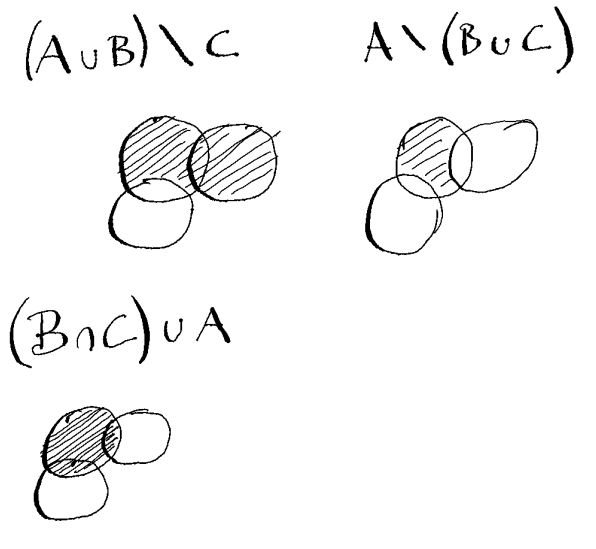
\includegraphics[width=0.3\textwidth]{img/dreiMeingenLoesung.png}
    \caption{Drei Mengen, Lösung. }
    \label{fig:dreiMengenLoes}
\end{figure}

\begin{figure}[h]
    \centering
    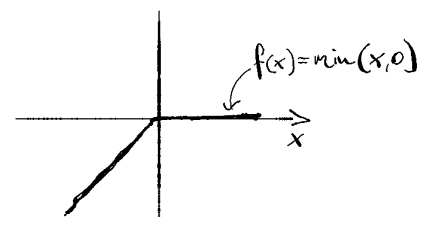
\includegraphics[width=0.3\textwidth]{img/loesung_min.png}
    \caption{Lösung. }
    \label{fig:Loes_min}
\end{figure}

\begin{figure}[h]
    \centering
    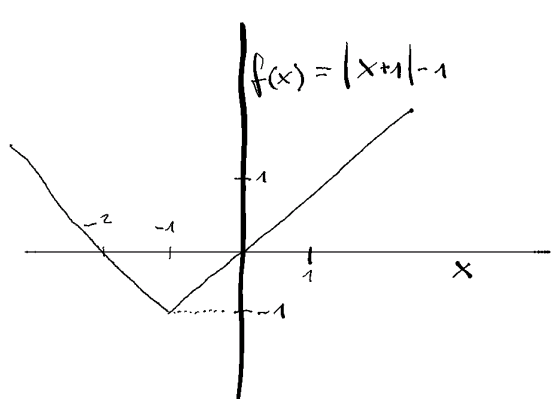
\includegraphics[width=0.3\textwidth]{img/loesung_abs.png}
    \caption{Lösung. }
    \label{fig:Loes_abs}
\end{figure}

\begin{figure}[h]
    \centering
    %% Creator: Matplotlib, PGF backend
%%
%% To include the figure in your LaTeX document, write
%%   \input{<filename>.pgf}
%%
%% Make sure the required packages are loaded in your preamble
%%   \usepackage{pgf}
%%
%% Also ensure that all the required font packages are loaded; for instance,
%% the lmodern package is sometimes necessary when using math font.
%%   \usepackage{lmodern}
%%
%% Figures using additional raster images can only be included by \input if
%% they are in the same directory as the main LaTeX file. For loading figures
%% from other directories you can use the `import` package
%%   \usepackage{import}
%%
%% and then include the figures with
%%   \import{<path to file>}{<filename>.pgf}
%%
%% Matplotlib used the following preamble
%%   \def\mathdefault#1{#1}
%%   \everymath=\expandafter{\the\everymath\displaystyle}
%%   
%%   \usepackage{fontspec}
%%   \setmainfont{VeraSe.ttf}[Path=\detokenize{/usr/share/fonts/TTF/}]
%%   \setsansfont{DejaVuSans.ttf}[Path=\detokenize{/home/pl/miniconda3/lib/python3.12/site-packages/matplotlib/mpl-data/fonts/ttf/}]
%%   \setmonofont{DejaVuSansMono.ttf}[Path=\detokenize{/home/pl/miniconda3/lib/python3.12/site-packages/matplotlib/mpl-data/fonts/ttf/}]
%%   \makeatletter\@ifpackageloaded{underscore}{}{\usepackage[strings]{underscore}}\makeatother
%%
\begingroup%
\makeatletter%
\begin{pgfpicture}%
\pgfpathrectangle{\pgfpointorigin}{\pgfqpoint{5.918612in}{3.167157in}}%
\pgfusepath{use as bounding box, clip}%
\begin{pgfscope}%
\pgfsetbuttcap%
\pgfsetmiterjoin%
\definecolor{currentfill}{rgb}{1.000000,1.000000,1.000000}%
\pgfsetfillcolor{currentfill}%
\pgfsetlinewidth{0.000000pt}%
\definecolor{currentstroke}{rgb}{1.000000,1.000000,1.000000}%
\pgfsetstrokecolor{currentstroke}%
\pgfsetdash{}{0pt}%
\pgfpathmoveto{\pgfqpoint{0.000000in}{0.000000in}}%
\pgfpathlineto{\pgfqpoint{5.918612in}{0.000000in}}%
\pgfpathlineto{\pgfqpoint{5.918612in}{3.167157in}}%
\pgfpathlineto{\pgfqpoint{0.000000in}{3.167157in}}%
\pgfpathlineto{\pgfqpoint{0.000000in}{0.000000in}}%
\pgfpathclose%
\pgfusepath{fill}%
\end{pgfscope}%
\begin{pgfscope}%
\pgfsetbuttcap%
\pgfsetmiterjoin%
\definecolor{currentfill}{rgb}{1.000000,1.000000,1.000000}%
\pgfsetfillcolor{currentfill}%
\pgfsetlinewidth{0.000000pt}%
\definecolor{currentstroke}{rgb}{0.000000,0.000000,0.000000}%
\pgfsetstrokecolor{currentstroke}%
\pgfsetstrokeopacity{0.000000}%
\pgfsetdash{}{0pt}%
\pgfpathmoveto{\pgfqpoint{0.393613in}{0.548486in}}%
\pgfpathlineto{\pgfqpoint{2.859522in}{0.548486in}}%
\pgfpathlineto{\pgfqpoint{2.859522in}{3.014395in}}%
\pgfpathlineto{\pgfqpoint{0.393613in}{3.014395in}}%
\pgfpathlineto{\pgfqpoint{0.393613in}{0.548486in}}%
\pgfpathclose%
\pgfusepath{fill}%
\end{pgfscope}%
\begin{pgfscope}%
\pgfsetbuttcap%
\pgfsetroundjoin%
\definecolor{currentfill}{rgb}{0.000000,0.000000,0.000000}%
\pgfsetfillcolor{currentfill}%
\pgfsetlinewidth{0.803000pt}%
\definecolor{currentstroke}{rgb}{0.000000,0.000000,0.000000}%
\pgfsetstrokecolor{currentstroke}%
\pgfsetdash{}{0pt}%
\pgfsys@defobject{currentmarker}{\pgfqpoint{0.000000in}{-0.048611in}}{\pgfqpoint{0.000000in}{0.000000in}}{%
\pgfpathmoveto{\pgfqpoint{0.000000in}{0.000000in}}%
\pgfpathlineto{\pgfqpoint{0.000000in}{-0.048611in}}%
\pgfusepath{stroke,fill}%
}%
\begin{pgfscope}%
\pgfsys@transformshift{0.804597in}{0.548486in}%
\pgfsys@useobject{currentmarker}{}%
\end{pgfscope}%
\end{pgfscope}%
\begin{pgfscope}%
\definecolor{textcolor}{rgb}{0.000000,0.000000,0.000000}%
\pgfsetstrokecolor{textcolor}%
\pgfsetfillcolor{textcolor}%
\pgftext[x=0.804597in,y=0.451264in,,top]{\color{textcolor}{\rmfamily\fontsize{10.000000}{12.000000}\selectfont\catcode`\^=\active\def^{\ifmmode\sp\else\^{}\fi}\catcode`\%=\active\def%{\%}\ensuremath{-}2}}%
\end{pgfscope}%
\begin{pgfscope}%
\pgfsetbuttcap%
\pgfsetroundjoin%
\definecolor{currentfill}{rgb}{0.000000,0.000000,0.000000}%
\pgfsetfillcolor{currentfill}%
\pgfsetlinewidth{0.803000pt}%
\definecolor{currentstroke}{rgb}{0.000000,0.000000,0.000000}%
\pgfsetstrokecolor{currentstroke}%
\pgfsetdash{}{0pt}%
\pgfsys@defobject{currentmarker}{\pgfqpoint{0.000000in}{-0.048611in}}{\pgfqpoint{0.000000in}{0.000000in}}{%
\pgfpathmoveto{\pgfqpoint{0.000000in}{0.000000in}}%
\pgfpathlineto{\pgfqpoint{0.000000in}{-0.048611in}}%
\pgfusepath{stroke,fill}%
}%
\begin{pgfscope}%
\pgfsys@transformshift{1.626567in}{0.548486in}%
\pgfsys@useobject{currentmarker}{}%
\end{pgfscope}%
\end{pgfscope}%
\begin{pgfscope}%
\definecolor{textcolor}{rgb}{0.000000,0.000000,0.000000}%
\pgfsetstrokecolor{textcolor}%
\pgfsetfillcolor{textcolor}%
\pgftext[x=1.626567in,y=0.451264in,,top]{\color{textcolor}{\rmfamily\fontsize{10.000000}{12.000000}\selectfont\catcode`\^=\active\def^{\ifmmode\sp\else\^{}\fi}\catcode`\%=\active\def%{\%}0}}%
\end{pgfscope}%
\begin{pgfscope}%
\pgfsetbuttcap%
\pgfsetroundjoin%
\definecolor{currentfill}{rgb}{0.000000,0.000000,0.000000}%
\pgfsetfillcolor{currentfill}%
\pgfsetlinewidth{0.803000pt}%
\definecolor{currentstroke}{rgb}{0.000000,0.000000,0.000000}%
\pgfsetstrokecolor{currentstroke}%
\pgfsetdash{}{0pt}%
\pgfsys@defobject{currentmarker}{\pgfqpoint{0.000000in}{-0.048611in}}{\pgfqpoint{0.000000in}{0.000000in}}{%
\pgfpathmoveto{\pgfqpoint{0.000000in}{0.000000in}}%
\pgfpathlineto{\pgfqpoint{0.000000in}{-0.048611in}}%
\pgfusepath{stroke,fill}%
}%
\begin{pgfscope}%
\pgfsys@transformshift{2.448537in}{0.548486in}%
\pgfsys@useobject{currentmarker}{}%
\end{pgfscope}%
\end{pgfscope}%
\begin{pgfscope}%
\definecolor{textcolor}{rgb}{0.000000,0.000000,0.000000}%
\pgfsetstrokecolor{textcolor}%
\pgfsetfillcolor{textcolor}%
\pgftext[x=2.448537in,y=0.451264in,,top]{\color{textcolor}{\rmfamily\fontsize{10.000000}{12.000000}\selectfont\catcode`\^=\active\def^{\ifmmode\sp\else\^{}\fi}\catcode`\%=\active\def%{\%}2}}%
\end{pgfscope}%
\begin{pgfscope}%
\definecolor{textcolor}{rgb}{0.000000,0.000000,0.000000}%
\pgfsetstrokecolor{textcolor}%
\pgfsetfillcolor{textcolor}%
\pgftext[x=1.626567in,y=0.261295in,,top]{\color{textcolor}{\rmfamily\fontsize{12.000000}{14.400000}\selectfont\catcode`\^=\active\def^{\ifmmode\sp\else\^{}\fi}\catcode`\%=\active\def%{\%}$x$}}%
\end{pgfscope}%
\begin{pgfscope}%
\pgfsetbuttcap%
\pgfsetroundjoin%
\definecolor{currentfill}{rgb}{0.000000,0.000000,0.000000}%
\pgfsetfillcolor{currentfill}%
\pgfsetlinewidth{0.803000pt}%
\definecolor{currentstroke}{rgb}{0.000000,0.000000,0.000000}%
\pgfsetstrokecolor{currentstroke}%
\pgfsetdash{}{0pt}%
\pgfsys@defobject{currentmarker}{\pgfqpoint{-0.048611in}{0.000000in}}{\pgfqpoint{-0.000000in}{0.000000in}}{%
\pgfpathmoveto{\pgfqpoint{-0.000000in}{0.000000in}}%
\pgfpathlineto{\pgfqpoint{-0.048611in}{0.000000in}}%
\pgfusepath{stroke,fill}%
}%
\begin{pgfscope}%
\pgfsys@transformshift{0.393613in}{0.548486in}%
\pgfsys@useobject{currentmarker}{}%
\end{pgfscope}%
\end{pgfscope}%
\begin{pgfscope}%
\definecolor{textcolor}{rgb}{0.000000,0.000000,0.000000}%
\pgfsetstrokecolor{textcolor}%
\pgfsetfillcolor{textcolor}%
\pgftext[x=0.100000in, y=0.495724in, left, base]{\color{textcolor}{\rmfamily\fontsize{10.000000}{12.000000}\selectfont\catcode`\^=\active\def^{\ifmmode\sp\else\^{}\fi}\catcode`\%=\active\def%{\%}\ensuremath{-}2}}%
\end{pgfscope}%
\begin{pgfscope}%
\pgfsetbuttcap%
\pgfsetroundjoin%
\definecolor{currentfill}{rgb}{0.000000,0.000000,0.000000}%
\pgfsetfillcolor{currentfill}%
\pgfsetlinewidth{0.803000pt}%
\definecolor{currentstroke}{rgb}{0.000000,0.000000,0.000000}%
\pgfsetstrokecolor{currentstroke}%
\pgfsetdash{}{0pt}%
\pgfsys@defobject{currentmarker}{\pgfqpoint{-0.048611in}{0.000000in}}{\pgfqpoint{-0.000000in}{0.000000in}}{%
\pgfpathmoveto{\pgfqpoint{-0.000000in}{0.000000in}}%
\pgfpathlineto{\pgfqpoint{-0.048611in}{0.000000in}}%
\pgfusepath{stroke,fill}%
}%
\begin{pgfscope}%
\pgfsys@transformshift{0.393613in}{0.959471in}%
\pgfsys@useobject{currentmarker}{}%
\end{pgfscope}%
\end{pgfscope}%
\begin{pgfscope}%
\definecolor{textcolor}{rgb}{0.000000,0.000000,0.000000}%
\pgfsetstrokecolor{textcolor}%
\pgfsetfillcolor{textcolor}%
\pgftext[x=0.100000in, y=0.906709in, left, base]{\color{textcolor}{\rmfamily\fontsize{10.000000}{12.000000}\selectfont\catcode`\^=\active\def^{\ifmmode\sp\else\^{}\fi}\catcode`\%=\active\def%{\%}\ensuremath{-}1}}%
\end{pgfscope}%
\begin{pgfscope}%
\pgfsetbuttcap%
\pgfsetroundjoin%
\definecolor{currentfill}{rgb}{0.000000,0.000000,0.000000}%
\pgfsetfillcolor{currentfill}%
\pgfsetlinewidth{0.803000pt}%
\definecolor{currentstroke}{rgb}{0.000000,0.000000,0.000000}%
\pgfsetstrokecolor{currentstroke}%
\pgfsetdash{}{0pt}%
\pgfsys@defobject{currentmarker}{\pgfqpoint{-0.048611in}{0.000000in}}{\pgfqpoint{-0.000000in}{0.000000in}}{%
\pgfpathmoveto{\pgfqpoint{-0.000000in}{0.000000in}}%
\pgfpathlineto{\pgfqpoint{-0.048611in}{0.000000in}}%
\pgfusepath{stroke,fill}%
}%
\begin{pgfscope}%
\pgfsys@transformshift{0.393613in}{1.370456in}%
\pgfsys@useobject{currentmarker}{}%
\end{pgfscope}%
\end{pgfscope}%
\begin{pgfscope}%
\definecolor{textcolor}{rgb}{0.000000,0.000000,0.000000}%
\pgfsetstrokecolor{textcolor}%
\pgfsetfillcolor{textcolor}%
\pgftext[x=0.208025in, y=1.317694in, left, base]{\color{textcolor}{\rmfamily\fontsize{10.000000}{12.000000}\selectfont\catcode`\^=\active\def^{\ifmmode\sp\else\^{}\fi}\catcode`\%=\active\def%{\%}0}}%
\end{pgfscope}%
\begin{pgfscope}%
\pgfsetbuttcap%
\pgfsetroundjoin%
\definecolor{currentfill}{rgb}{0.000000,0.000000,0.000000}%
\pgfsetfillcolor{currentfill}%
\pgfsetlinewidth{0.803000pt}%
\definecolor{currentstroke}{rgb}{0.000000,0.000000,0.000000}%
\pgfsetstrokecolor{currentstroke}%
\pgfsetdash{}{0pt}%
\pgfsys@defobject{currentmarker}{\pgfqpoint{-0.048611in}{0.000000in}}{\pgfqpoint{-0.000000in}{0.000000in}}{%
\pgfpathmoveto{\pgfqpoint{-0.000000in}{0.000000in}}%
\pgfpathlineto{\pgfqpoint{-0.048611in}{0.000000in}}%
\pgfusepath{stroke,fill}%
}%
\begin{pgfscope}%
\pgfsys@transformshift{0.393613in}{1.781441in}%
\pgfsys@useobject{currentmarker}{}%
\end{pgfscope}%
\end{pgfscope}%
\begin{pgfscope}%
\definecolor{textcolor}{rgb}{0.000000,0.000000,0.000000}%
\pgfsetstrokecolor{textcolor}%
\pgfsetfillcolor{textcolor}%
\pgftext[x=0.208025in, y=1.728679in, left, base]{\color{textcolor}{\rmfamily\fontsize{10.000000}{12.000000}\selectfont\catcode`\^=\active\def^{\ifmmode\sp\else\^{}\fi}\catcode`\%=\active\def%{\%}1}}%
\end{pgfscope}%
\begin{pgfscope}%
\pgfsetbuttcap%
\pgfsetroundjoin%
\definecolor{currentfill}{rgb}{0.000000,0.000000,0.000000}%
\pgfsetfillcolor{currentfill}%
\pgfsetlinewidth{0.803000pt}%
\definecolor{currentstroke}{rgb}{0.000000,0.000000,0.000000}%
\pgfsetstrokecolor{currentstroke}%
\pgfsetdash{}{0pt}%
\pgfsys@defobject{currentmarker}{\pgfqpoint{-0.048611in}{0.000000in}}{\pgfqpoint{-0.000000in}{0.000000in}}{%
\pgfpathmoveto{\pgfqpoint{-0.000000in}{0.000000in}}%
\pgfpathlineto{\pgfqpoint{-0.048611in}{0.000000in}}%
\pgfusepath{stroke,fill}%
}%
\begin{pgfscope}%
\pgfsys@transformshift{0.393613in}{2.192425in}%
\pgfsys@useobject{currentmarker}{}%
\end{pgfscope}%
\end{pgfscope}%
\begin{pgfscope}%
\definecolor{textcolor}{rgb}{0.000000,0.000000,0.000000}%
\pgfsetstrokecolor{textcolor}%
\pgfsetfillcolor{textcolor}%
\pgftext[x=0.208025in, y=2.139664in, left, base]{\color{textcolor}{\rmfamily\fontsize{10.000000}{12.000000}\selectfont\catcode`\^=\active\def^{\ifmmode\sp\else\^{}\fi}\catcode`\%=\active\def%{\%}2}}%
\end{pgfscope}%
\begin{pgfscope}%
\pgfsetbuttcap%
\pgfsetroundjoin%
\definecolor{currentfill}{rgb}{0.000000,0.000000,0.000000}%
\pgfsetfillcolor{currentfill}%
\pgfsetlinewidth{0.803000pt}%
\definecolor{currentstroke}{rgb}{0.000000,0.000000,0.000000}%
\pgfsetstrokecolor{currentstroke}%
\pgfsetdash{}{0pt}%
\pgfsys@defobject{currentmarker}{\pgfqpoint{-0.048611in}{0.000000in}}{\pgfqpoint{-0.000000in}{0.000000in}}{%
\pgfpathmoveto{\pgfqpoint{-0.000000in}{0.000000in}}%
\pgfpathlineto{\pgfqpoint{-0.048611in}{0.000000in}}%
\pgfusepath{stroke,fill}%
}%
\begin{pgfscope}%
\pgfsys@transformshift{0.393613in}{2.603410in}%
\pgfsys@useobject{currentmarker}{}%
\end{pgfscope}%
\end{pgfscope}%
\begin{pgfscope}%
\definecolor{textcolor}{rgb}{0.000000,0.000000,0.000000}%
\pgfsetstrokecolor{textcolor}%
\pgfsetfillcolor{textcolor}%
\pgftext[x=0.208025in, y=2.550649in, left, base]{\color{textcolor}{\rmfamily\fontsize{10.000000}{12.000000}\selectfont\catcode`\^=\active\def^{\ifmmode\sp\else\^{}\fi}\catcode`\%=\active\def%{\%}3}}%
\end{pgfscope}%
\begin{pgfscope}%
\pgfsetbuttcap%
\pgfsetroundjoin%
\definecolor{currentfill}{rgb}{0.000000,0.000000,0.000000}%
\pgfsetfillcolor{currentfill}%
\pgfsetlinewidth{0.803000pt}%
\definecolor{currentstroke}{rgb}{0.000000,0.000000,0.000000}%
\pgfsetstrokecolor{currentstroke}%
\pgfsetdash{}{0pt}%
\pgfsys@defobject{currentmarker}{\pgfqpoint{-0.048611in}{0.000000in}}{\pgfqpoint{-0.000000in}{0.000000in}}{%
\pgfpathmoveto{\pgfqpoint{-0.000000in}{0.000000in}}%
\pgfpathlineto{\pgfqpoint{-0.048611in}{0.000000in}}%
\pgfusepath{stroke,fill}%
}%
\begin{pgfscope}%
\pgfsys@transformshift{0.393613in}{3.014395in}%
\pgfsys@useobject{currentmarker}{}%
\end{pgfscope}%
\end{pgfscope}%
\begin{pgfscope}%
\definecolor{textcolor}{rgb}{0.000000,0.000000,0.000000}%
\pgfsetstrokecolor{textcolor}%
\pgfsetfillcolor{textcolor}%
\pgftext[x=0.208025in, y=2.961634in, left, base]{\color{textcolor}{\rmfamily\fontsize{10.000000}{12.000000}\selectfont\catcode`\^=\active\def^{\ifmmode\sp\else\^{}\fi}\catcode`\%=\active\def%{\%}4}}%
\end{pgfscope}%
\begin{pgfscope}%
\pgfpathrectangle{\pgfqpoint{0.393613in}{0.548486in}}{\pgfqpoint{2.465909in}{2.465909in}}%
\pgfusepath{clip}%
\pgfsetrectcap%
\pgfsetroundjoin%
\pgfsetlinewidth{1.505625pt}%
\definecolor{currentstroke}{rgb}{0.000000,0.000000,0.000000}%
\pgfsetstrokecolor{currentstroke}%
\pgfsetdash{}{0pt}%
\pgfpathmoveto{\pgfqpoint{0.393613in}{3.014395in}}%
\pgfpathlineto{\pgfqpoint{0.418521in}{2.989487in}}%
\pgfpathlineto{\pgfqpoint{0.443429in}{2.964579in}}%
\pgfpathlineto{\pgfqpoint{0.468337in}{2.939671in}}%
\pgfpathlineto{\pgfqpoint{0.493245in}{2.914762in}}%
\pgfpathlineto{\pgfqpoint{0.518153in}{2.889854in}}%
\pgfpathlineto{\pgfqpoint{0.543062in}{2.864946in}}%
\pgfpathlineto{\pgfqpoint{0.567970in}{2.840038in}}%
\pgfpathlineto{\pgfqpoint{0.592878in}{2.815130in}}%
\pgfpathlineto{\pgfqpoint{0.617786in}{2.790222in}}%
\pgfpathlineto{\pgfqpoint{0.642694in}{2.765313in}}%
\pgfpathlineto{\pgfqpoint{0.667602in}{2.740405in}}%
\pgfpathlineto{\pgfqpoint{0.692511in}{2.715497in}}%
\pgfpathlineto{\pgfqpoint{0.717419in}{2.690589in}}%
\pgfpathlineto{\pgfqpoint{0.742327in}{2.665681in}}%
\pgfpathlineto{\pgfqpoint{0.767235in}{2.640772in}}%
\pgfpathlineto{\pgfqpoint{0.792143in}{2.615864in}}%
\pgfpathlineto{\pgfqpoint{0.817051in}{2.590956in}}%
\pgfpathlineto{\pgfqpoint{0.841960in}{2.566048in}}%
\pgfpathlineto{\pgfqpoint{0.866868in}{2.541140in}}%
\pgfpathlineto{\pgfqpoint{0.891776in}{2.516232in}}%
\pgfpathlineto{\pgfqpoint{0.916684in}{2.491323in}}%
\pgfpathlineto{\pgfqpoint{0.941592in}{2.466415in}}%
\pgfpathlineto{\pgfqpoint{0.966500in}{2.441507in}}%
\pgfpathlineto{\pgfqpoint{0.991409in}{2.416599in}}%
\pgfpathlineto{\pgfqpoint{1.016317in}{2.391691in}}%
\pgfpathlineto{\pgfqpoint{1.041225in}{2.366783in}}%
\pgfpathlineto{\pgfqpoint{1.066133in}{2.341874in}}%
\pgfpathlineto{\pgfqpoint{1.091041in}{2.316966in}}%
\pgfpathlineto{\pgfqpoint{1.115950in}{2.292058in}}%
\pgfpathlineto{\pgfqpoint{1.140858in}{2.267150in}}%
\pgfpathlineto{\pgfqpoint{1.165766in}{2.242242in}}%
\pgfpathlineto{\pgfqpoint{1.190674in}{2.217334in}}%
\pgfpathlineto{\pgfqpoint{1.215582in}{2.192425in}}%
\pgfpathlineto{\pgfqpoint{1.240490in}{2.167517in}}%
\pgfpathlineto{\pgfqpoint{1.265399in}{2.142609in}}%
\pgfpathlineto{\pgfqpoint{1.290307in}{2.117701in}}%
\pgfpathlineto{\pgfqpoint{1.315215in}{2.092793in}}%
\pgfpathlineto{\pgfqpoint{1.340123in}{2.067885in}}%
\pgfpathlineto{\pgfqpoint{1.365031in}{2.042976in}}%
\pgfpathlineto{\pgfqpoint{1.389939in}{2.018068in}}%
\pgfpathlineto{\pgfqpoint{1.414848in}{1.993160in}}%
\pgfpathlineto{\pgfqpoint{1.439756in}{1.968252in}}%
\pgfpathlineto{\pgfqpoint{1.464664in}{1.943344in}}%
\pgfpathlineto{\pgfqpoint{1.489572in}{1.918435in}}%
\pgfpathlineto{\pgfqpoint{1.514480in}{1.893527in}}%
\pgfpathlineto{\pgfqpoint{1.539388in}{1.868619in}}%
\pgfpathlineto{\pgfqpoint{1.564297in}{1.843711in}}%
\pgfpathlineto{\pgfqpoint{1.589205in}{1.818803in}}%
\pgfpathlineto{\pgfqpoint{1.614113in}{1.793895in}}%
\pgfpathlineto{\pgfqpoint{1.639021in}{1.768986in}}%
\pgfpathlineto{\pgfqpoint{1.663929in}{1.744078in}}%
\pgfpathlineto{\pgfqpoint{1.688837in}{1.719170in}}%
\pgfpathlineto{\pgfqpoint{1.713746in}{1.694262in}}%
\pgfpathlineto{\pgfqpoint{1.738654in}{1.669354in}}%
\pgfpathlineto{\pgfqpoint{1.763562in}{1.644446in}}%
\pgfpathlineto{\pgfqpoint{1.788470in}{1.619537in}}%
\pgfpathlineto{\pgfqpoint{1.813378in}{1.594629in}}%
\pgfpathlineto{\pgfqpoint{1.838287in}{1.569721in}}%
\pgfpathlineto{\pgfqpoint{1.863195in}{1.544813in}}%
\pgfpathlineto{\pgfqpoint{1.888103in}{1.519905in}}%
\pgfpathlineto{\pgfqpoint{1.913011in}{1.494997in}}%
\pgfpathlineto{\pgfqpoint{1.937919in}{1.470088in}}%
\pgfpathlineto{\pgfqpoint{1.962827in}{1.445180in}}%
\pgfpathlineto{\pgfqpoint{1.987736in}{1.420272in}}%
\pgfpathlineto{\pgfqpoint{2.012644in}{1.395364in}}%
\pgfpathlineto{\pgfqpoint{2.037552in}{1.370456in}}%
\pgfpathlineto{\pgfqpoint{2.062460in}{1.345547in}}%
\pgfpathlineto{\pgfqpoint{2.087368in}{1.320639in}}%
\pgfpathlineto{\pgfqpoint{2.112276in}{1.295731in}}%
\pgfpathlineto{\pgfqpoint{2.137185in}{1.270823in}}%
\pgfpathlineto{\pgfqpoint{2.162093in}{1.245915in}}%
\pgfpathlineto{\pgfqpoint{2.187001in}{1.221007in}}%
\pgfpathlineto{\pgfqpoint{2.211909in}{1.196098in}}%
\pgfpathlineto{\pgfqpoint{2.236817in}{1.171190in}}%
\pgfpathlineto{\pgfqpoint{2.261725in}{1.146282in}}%
\pgfpathlineto{\pgfqpoint{2.286634in}{1.121374in}}%
\pgfpathlineto{\pgfqpoint{2.311542in}{1.096466in}}%
\pgfpathlineto{\pgfqpoint{2.336450in}{1.071558in}}%
\pgfpathlineto{\pgfqpoint{2.361358in}{1.046649in}}%
\pgfpathlineto{\pgfqpoint{2.386266in}{1.021741in}}%
\pgfpathlineto{\pgfqpoint{2.411174in}{0.996833in}}%
\pgfpathlineto{\pgfqpoint{2.436083in}{0.971925in}}%
\pgfpathlineto{\pgfqpoint{2.460991in}{0.971925in}}%
\pgfpathlineto{\pgfqpoint{2.485899in}{0.996833in}}%
\pgfpathlineto{\pgfqpoint{2.510807in}{1.021741in}}%
\pgfpathlineto{\pgfqpoint{2.535715in}{1.046649in}}%
\pgfpathlineto{\pgfqpoint{2.560624in}{1.071558in}}%
\pgfpathlineto{\pgfqpoint{2.585532in}{1.096466in}}%
\pgfpathlineto{\pgfqpoint{2.610440in}{1.121374in}}%
\pgfpathlineto{\pgfqpoint{2.635348in}{1.146282in}}%
\pgfpathlineto{\pgfqpoint{2.660256in}{1.171190in}}%
\pgfpathlineto{\pgfqpoint{2.685164in}{1.196098in}}%
\pgfpathlineto{\pgfqpoint{2.710073in}{1.221007in}}%
\pgfpathlineto{\pgfqpoint{2.734981in}{1.245915in}}%
\pgfpathlineto{\pgfqpoint{2.759889in}{1.270823in}}%
\pgfpathlineto{\pgfqpoint{2.784797in}{1.295731in}}%
\pgfpathlineto{\pgfqpoint{2.809705in}{1.320639in}}%
\pgfpathlineto{\pgfqpoint{2.834613in}{1.345547in}}%
\pgfpathlineto{\pgfqpoint{2.859522in}{1.370456in}}%
\pgfusepath{stroke}%
\end{pgfscope}%
\begin{pgfscope}%
\pgfpathrectangle{\pgfqpoint{0.393613in}{0.548486in}}{\pgfqpoint{2.465909in}{2.465909in}}%
\pgfusepath{clip}%
\pgfsetbuttcap%
\pgfsetroundjoin%
\pgfsetlinewidth{1.505625pt}%
\definecolor{currentstroke}{rgb}{0.000000,0.000000,0.000000}%
\pgfsetstrokecolor{currentstroke}%
\pgfsetdash{{5.550000pt}{2.400000pt}}{0.000000pt}%
\pgfpathmoveto{\pgfqpoint{0.393613in}{2.603410in}}%
\pgfpathlineto{\pgfqpoint{0.418521in}{2.578502in}}%
\pgfpathlineto{\pgfqpoint{0.443429in}{2.553594in}}%
\pgfpathlineto{\pgfqpoint{0.468337in}{2.528686in}}%
\pgfpathlineto{\pgfqpoint{0.493245in}{2.503778in}}%
\pgfpathlineto{\pgfqpoint{0.518153in}{2.478869in}}%
\pgfpathlineto{\pgfqpoint{0.543062in}{2.453961in}}%
\pgfpathlineto{\pgfqpoint{0.567970in}{2.429053in}}%
\pgfpathlineto{\pgfqpoint{0.592878in}{2.404145in}}%
\pgfpathlineto{\pgfqpoint{0.617786in}{2.379237in}}%
\pgfpathlineto{\pgfqpoint{0.642694in}{2.354328in}}%
\pgfpathlineto{\pgfqpoint{0.667602in}{2.329420in}}%
\pgfpathlineto{\pgfqpoint{0.692511in}{2.304512in}}%
\pgfpathlineto{\pgfqpoint{0.717419in}{2.279604in}}%
\pgfpathlineto{\pgfqpoint{0.742327in}{2.254696in}}%
\pgfpathlineto{\pgfqpoint{0.767235in}{2.229788in}}%
\pgfpathlineto{\pgfqpoint{0.792143in}{2.204879in}}%
\pgfpathlineto{\pgfqpoint{0.817051in}{2.179971in}}%
\pgfpathlineto{\pgfqpoint{0.841960in}{2.155063in}}%
\pgfpathlineto{\pgfqpoint{0.866868in}{2.130155in}}%
\pgfpathlineto{\pgfqpoint{0.891776in}{2.105247in}}%
\pgfpathlineto{\pgfqpoint{0.916684in}{2.080339in}}%
\pgfpathlineto{\pgfqpoint{0.941592in}{2.055430in}}%
\pgfpathlineto{\pgfqpoint{0.966500in}{2.030522in}}%
\pgfpathlineto{\pgfqpoint{0.991409in}{2.005614in}}%
\pgfpathlineto{\pgfqpoint{1.016317in}{1.980706in}}%
\pgfpathlineto{\pgfqpoint{1.041225in}{1.955798in}}%
\pgfpathlineto{\pgfqpoint{1.066133in}{1.930890in}}%
\pgfpathlineto{\pgfqpoint{1.091041in}{1.905981in}}%
\pgfpathlineto{\pgfqpoint{1.115950in}{1.881073in}}%
\pgfpathlineto{\pgfqpoint{1.140858in}{1.856165in}}%
\pgfpathlineto{\pgfqpoint{1.165766in}{1.831257in}}%
\pgfpathlineto{\pgfqpoint{1.190674in}{1.806349in}}%
\pgfpathlineto{\pgfqpoint{1.215582in}{1.781441in}}%
\pgfpathlineto{\pgfqpoint{1.240490in}{1.756532in}}%
\pgfpathlineto{\pgfqpoint{1.265399in}{1.731624in}}%
\pgfpathlineto{\pgfqpoint{1.290307in}{1.706716in}}%
\pgfpathlineto{\pgfqpoint{1.315215in}{1.681808in}}%
\pgfpathlineto{\pgfqpoint{1.340123in}{1.656900in}}%
\pgfpathlineto{\pgfqpoint{1.365031in}{1.631991in}}%
\pgfpathlineto{\pgfqpoint{1.389939in}{1.607083in}}%
\pgfpathlineto{\pgfqpoint{1.414848in}{1.582175in}}%
\pgfpathlineto{\pgfqpoint{1.439756in}{1.557267in}}%
\pgfpathlineto{\pgfqpoint{1.464664in}{1.532359in}}%
\pgfpathlineto{\pgfqpoint{1.489572in}{1.507451in}}%
\pgfpathlineto{\pgfqpoint{1.514480in}{1.482542in}}%
\pgfpathlineto{\pgfqpoint{1.539388in}{1.457634in}}%
\pgfpathlineto{\pgfqpoint{1.564297in}{1.432726in}}%
\pgfpathlineto{\pgfqpoint{1.589205in}{1.407818in}}%
\pgfpathlineto{\pgfqpoint{1.614113in}{1.382910in}}%
\pgfpathlineto{\pgfqpoint{1.639021in}{1.358002in}}%
\pgfpathlineto{\pgfqpoint{1.663929in}{1.333093in}}%
\pgfpathlineto{\pgfqpoint{1.688837in}{1.308185in}}%
\pgfpathlineto{\pgfqpoint{1.713746in}{1.283277in}}%
\pgfpathlineto{\pgfqpoint{1.738654in}{1.258369in}}%
\pgfpathlineto{\pgfqpoint{1.763562in}{1.233461in}}%
\pgfpathlineto{\pgfqpoint{1.788470in}{1.208553in}}%
\pgfpathlineto{\pgfqpoint{1.813378in}{1.183644in}}%
\pgfpathlineto{\pgfqpoint{1.838287in}{1.158736in}}%
\pgfpathlineto{\pgfqpoint{1.863195in}{1.133828in}}%
\pgfpathlineto{\pgfqpoint{1.888103in}{1.108920in}}%
\pgfpathlineto{\pgfqpoint{1.913011in}{1.084012in}}%
\pgfpathlineto{\pgfqpoint{1.937919in}{1.059104in}}%
\pgfpathlineto{\pgfqpoint{1.962827in}{1.034195in}}%
\pgfpathlineto{\pgfqpoint{1.987736in}{1.009287in}}%
\pgfpathlineto{\pgfqpoint{2.012644in}{0.984379in}}%
\pgfpathlineto{\pgfqpoint{2.037552in}{0.959471in}}%
\pgfpathlineto{\pgfqpoint{2.062460in}{0.984379in}}%
\pgfpathlineto{\pgfqpoint{2.087368in}{1.009287in}}%
\pgfpathlineto{\pgfqpoint{2.112276in}{1.034195in}}%
\pgfpathlineto{\pgfqpoint{2.137185in}{1.059104in}}%
\pgfpathlineto{\pgfqpoint{2.162093in}{1.084012in}}%
\pgfpathlineto{\pgfqpoint{2.187001in}{1.108920in}}%
\pgfpathlineto{\pgfqpoint{2.211909in}{1.133828in}}%
\pgfpathlineto{\pgfqpoint{2.236817in}{1.158736in}}%
\pgfpathlineto{\pgfqpoint{2.261725in}{1.183644in}}%
\pgfpathlineto{\pgfqpoint{2.286634in}{1.208553in}}%
\pgfpathlineto{\pgfqpoint{2.311542in}{1.233461in}}%
\pgfpathlineto{\pgfqpoint{2.336450in}{1.258369in}}%
\pgfpathlineto{\pgfqpoint{2.361358in}{1.283277in}}%
\pgfpathlineto{\pgfqpoint{2.386266in}{1.308185in}}%
\pgfpathlineto{\pgfqpoint{2.411174in}{1.333093in}}%
\pgfpathlineto{\pgfqpoint{2.436083in}{1.358002in}}%
\pgfpathlineto{\pgfqpoint{2.460991in}{1.382910in}}%
\pgfpathlineto{\pgfqpoint{2.485899in}{1.407818in}}%
\pgfpathlineto{\pgfqpoint{2.510807in}{1.432726in}}%
\pgfpathlineto{\pgfqpoint{2.535715in}{1.457634in}}%
\pgfpathlineto{\pgfqpoint{2.560624in}{1.482542in}}%
\pgfpathlineto{\pgfqpoint{2.585532in}{1.507451in}}%
\pgfpathlineto{\pgfqpoint{2.610440in}{1.532359in}}%
\pgfpathlineto{\pgfqpoint{2.635348in}{1.557267in}}%
\pgfpathlineto{\pgfqpoint{2.660256in}{1.582175in}}%
\pgfpathlineto{\pgfqpoint{2.685164in}{1.607083in}}%
\pgfpathlineto{\pgfqpoint{2.710073in}{1.631991in}}%
\pgfpathlineto{\pgfqpoint{2.734981in}{1.656900in}}%
\pgfpathlineto{\pgfqpoint{2.759889in}{1.681808in}}%
\pgfpathlineto{\pgfqpoint{2.784797in}{1.706716in}}%
\pgfpathlineto{\pgfqpoint{2.809705in}{1.731624in}}%
\pgfpathlineto{\pgfqpoint{2.834613in}{1.756532in}}%
\pgfpathlineto{\pgfqpoint{2.859522in}{1.781441in}}%
\pgfusepath{stroke}%
\end{pgfscope}%
\begin{pgfscope}%
\pgfpathrectangle{\pgfqpoint{0.393613in}{0.548486in}}{\pgfqpoint{2.465909in}{2.465909in}}%
\pgfusepath{clip}%
\pgfsetrectcap%
\pgfsetroundjoin%
\pgfsetlinewidth{1.505625pt}%
\definecolor{currentstroke}{rgb}{1.000000,0.000000,0.000000}%
\pgfsetstrokecolor{currentstroke}%
\pgfsetdash{}{0pt}%
\pgfpathmoveto{\pgfqpoint{0.393613in}{2.192425in}}%
\pgfpathlineto{\pgfqpoint{0.418521in}{2.167517in}}%
\pgfpathlineto{\pgfqpoint{0.443429in}{2.142609in}}%
\pgfpathlineto{\pgfqpoint{0.468337in}{2.117701in}}%
\pgfpathlineto{\pgfqpoint{0.493245in}{2.092793in}}%
\pgfpathlineto{\pgfqpoint{0.518153in}{2.067885in}}%
\pgfpathlineto{\pgfqpoint{0.543062in}{2.042976in}}%
\pgfpathlineto{\pgfqpoint{0.567970in}{2.018068in}}%
\pgfpathlineto{\pgfqpoint{0.592878in}{1.993160in}}%
\pgfpathlineto{\pgfqpoint{0.617786in}{1.968252in}}%
\pgfpathlineto{\pgfqpoint{0.642694in}{1.943344in}}%
\pgfpathlineto{\pgfqpoint{0.667602in}{1.918435in}}%
\pgfpathlineto{\pgfqpoint{0.692511in}{1.893527in}}%
\pgfpathlineto{\pgfqpoint{0.717419in}{1.868619in}}%
\pgfpathlineto{\pgfqpoint{0.742327in}{1.843711in}}%
\pgfpathlineto{\pgfqpoint{0.767235in}{1.818803in}}%
\pgfpathlineto{\pgfqpoint{0.792143in}{1.793895in}}%
\pgfpathlineto{\pgfqpoint{0.817051in}{1.768986in}}%
\pgfpathlineto{\pgfqpoint{0.841960in}{1.744078in}}%
\pgfpathlineto{\pgfqpoint{0.866868in}{1.719170in}}%
\pgfpathlineto{\pgfqpoint{0.891776in}{1.694262in}}%
\pgfpathlineto{\pgfqpoint{0.916684in}{1.669354in}}%
\pgfpathlineto{\pgfqpoint{0.941592in}{1.644446in}}%
\pgfpathlineto{\pgfqpoint{0.966500in}{1.619537in}}%
\pgfpathlineto{\pgfqpoint{0.991409in}{1.594629in}}%
\pgfpathlineto{\pgfqpoint{1.016317in}{1.569721in}}%
\pgfpathlineto{\pgfqpoint{1.041225in}{1.544813in}}%
\pgfpathlineto{\pgfqpoint{1.066133in}{1.519905in}}%
\pgfpathlineto{\pgfqpoint{1.091041in}{1.494997in}}%
\pgfpathlineto{\pgfqpoint{1.115950in}{1.470088in}}%
\pgfpathlineto{\pgfqpoint{1.140858in}{1.445180in}}%
\pgfpathlineto{\pgfqpoint{1.165766in}{1.420272in}}%
\pgfpathlineto{\pgfqpoint{1.190674in}{1.395364in}}%
\pgfpathlineto{\pgfqpoint{1.215582in}{1.370456in}}%
\pgfpathlineto{\pgfqpoint{1.240490in}{1.345547in}}%
\pgfpathlineto{\pgfqpoint{1.265399in}{1.320639in}}%
\pgfpathlineto{\pgfqpoint{1.290307in}{1.295731in}}%
\pgfpathlineto{\pgfqpoint{1.315215in}{1.270823in}}%
\pgfpathlineto{\pgfqpoint{1.340123in}{1.245915in}}%
\pgfpathlineto{\pgfqpoint{1.365031in}{1.221007in}}%
\pgfpathlineto{\pgfqpoint{1.389939in}{1.196098in}}%
\pgfpathlineto{\pgfqpoint{1.414848in}{1.171190in}}%
\pgfpathlineto{\pgfqpoint{1.439756in}{1.146282in}}%
\pgfpathlineto{\pgfqpoint{1.464664in}{1.121374in}}%
\pgfpathlineto{\pgfqpoint{1.489572in}{1.096466in}}%
\pgfpathlineto{\pgfqpoint{1.514480in}{1.071558in}}%
\pgfpathlineto{\pgfqpoint{1.539388in}{1.046649in}}%
\pgfpathlineto{\pgfqpoint{1.564297in}{1.021741in}}%
\pgfpathlineto{\pgfqpoint{1.589205in}{0.996833in}}%
\pgfpathlineto{\pgfqpoint{1.614113in}{0.971925in}}%
\pgfpathlineto{\pgfqpoint{1.639021in}{0.971925in}}%
\pgfpathlineto{\pgfqpoint{1.663929in}{0.996833in}}%
\pgfpathlineto{\pgfqpoint{1.688837in}{1.021741in}}%
\pgfpathlineto{\pgfqpoint{1.713746in}{1.046649in}}%
\pgfpathlineto{\pgfqpoint{1.738654in}{1.071558in}}%
\pgfpathlineto{\pgfqpoint{1.763562in}{1.096466in}}%
\pgfpathlineto{\pgfqpoint{1.788470in}{1.121374in}}%
\pgfpathlineto{\pgfqpoint{1.813378in}{1.146282in}}%
\pgfpathlineto{\pgfqpoint{1.838287in}{1.171190in}}%
\pgfpathlineto{\pgfqpoint{1.863195in}{1.196098in}}%
\pgfpathlineto{\pgfqpoint{1.888103in}{1.221007in}}%
\pgfpathlineto{\pgfqpoint{1.913011in}{1.245915in}}%
\pgfpathlineto{\pgfqpoint{1.937919in}{1.270823in}}%
\pgfpathlineto{\pgfqpoint{1.962827in}{1.295731in}}%
\pgfpathlineto{\pgfqpoint{1.987736in}{1.320639in}}%
\pgfpathlineto{\pgfqpoint{2.012644in}{1.345547in}}%
\pgfpathlineto{\pgfqpoint{2.037552in}{1.370456in}}%
\pgfpathlineto{\pgfqpoint{2.062460in}{1.395364in}}%
\pgfpathlineto{\pgfqpoint{2.087368in}{1.420272in}}%
\pgfpathlineto{\pgfqpoint{2.112276in}{1.445180in}}%
\pgfpathlineto{\pgfqpoint{2.137185in}{1.470088in}}%
\pgfpathlineto{\pgfqpoint{2.162093in}{1.494997in}}%
\pgfpathlineto{\pgfqpoint{2.187001in}{1.519905in}}%
\pgfpathlineto{\pgfqpoint{2.211909in}{1.544813in}}%
\pgfpathlineto{\pgfqpoint{2.236817in}{1.569721in}}%
\pgfpathlineto{\pgfqpoint{2.261725in}{1.594629in}}%
\pgfpathlineto{\pgfqpoint{2.286634in}{1.619537in}}%
\pgfpathlineto{\pgfqpoint{2.311542in}{1.644446in}}%
\pgfpathlineto{\pgfqpoint{2.336450in}{1.669354in}}%
\pgfpathlineto{\pgfqpoint{2.361358in}{1.694262in}}%
\pgfpathlineto{\pgfqpoint{2.386266in}{1.719170in}}%
\pgfpathlineto{\pgfqpoint{2.411174in}{1.744078in}}%
\pgfpathlineto{\pgfqpoint{2.436083in}{1.768986in}}%
\pgfpathlineto{\pgfqpoint{2.460991in}{1.793895in}}%
\pgfpathlineto{\pgfqpoint{2.485899in}{1.818803in}}%
\pgfpathlineto{\pgfqpoint{2.510807in}{1.843711in}}%
\pgfpathlineto{\pgfqpoint{2.535715in}{1.868619in}}%
\pgfpathlineto{\pgfqpoint{2.560624in}{1.893527in}}%
\pgfpathlineto{\pgfqpoint{2.585532in}{1.918435in}}%
\pgfpathlineto{\pgfqpoint{2.610440in}{1.943344in}}%
\pgfpathlineto{\pgfqpoint{2.635348in}{1.968252in}}%
\pgfpathlineto{\pgfqpoint{2.660256in}{1.993160in}}%
\pgfpathlineto{\pgfqpoint{2.685164in}{2.018068in}}%
\pgfpathlineto{\pgfqpoint{2.710073in}{2.042976in}}%
\pgfpathlineto{\pgfqpoint{2.734981in}{2.067885in}}%
\pgfpathlineto{\pgfqpoint{2.759889in}{2.092793in}}%
\pgfpathlineto{\pgfqpoint{2.784797in}{2.117701in}}%
\pgfpathlineto{\pgfqpoint{2.809705in}{2.142609in}}%
\pgfpathlineto{\pgfqpoint{2.834613in}{2.167517in}}%
\pgfpathlineto{\pgfqpoint{2.859522in}{2.192425in}}%
\pgfusepath{stroke}%
\end{pgfscope}%
\begin{pgfscope}%
\pgfpathrectangle{\pgfqpoint{0.393613in}{0.548486in}}{\pgfqpoint{2.465909in}{2.465909in}}%
\pgfusepath{clip}%
\pgfsetbuttcap%
\pgfsetroundjoin%
\pgfsetlinewidth{1.505625pt}%
\definecolor{currentstroke}{rgb}{1.000000,0.000000,0.000000}%
\pgfsetstrokecolor{currentstroke}%
\pgfsetdash{{5.550000pt}{2.400000pt}}{0.000000pt}%
\pgfpathmoveto{\pgfqpoint{0.393613in}{1.781441in}}%
\pgfpathlineto{\pgfqpoint{0.418521in}{1.756532in}}%
\pgfpathlineto{\pgfqpoint{0.443429in}{1.731624in}}%
\pgfpathlineto{\pgfqpoint{0.468337in}{1.706716in}}%
\pgfpathlineto{\pgfqpoint{0.493245in}{1.681808in}}%
\pgfpathlineto{\pgfqpoint{0.518153in}{1.656900in}}%
\pgfpathlineto{\pgfqpoint{0.543062in}{1.631991in}}%
\pgfpathlineto{\pgfqpoint{0.567970in}{1.607083in}}%
\pgfpathlineto{\pgfqpoint{0.592878in}{1.582175in}}%
\pgfpathlineto{\pgfqpoint{0.617786in}{1.557267in}}%
\pgfpathlineto{\pgfqpoint{0.642694in}{1.532359in}}%
\pgfpathlineto{\pgfqpoint{0.667602in}{1.507451in}}%
\pgfpathlineto{\pgfqpoint{0.692511in}{1.482542in}}%
\pgfpathlineto{\pgfqpoint{0.717419in}{1.457634in}}%
\pgfpathlineto{\pgfqpoint{0.742327in}{1.432726in}}%
\pgfpathlineto{\pgfqpoint{0.767235in}{1.407818in}}%
\pgfpathlineto{\pgfqpoint{0.792143in}{1.382910in}}%
\pgfpathlineto{\pgfqpoint{0.817051in}{1.358002in}}%
\pgfpathlineto{\pgfqpoint{0.841960in}{1.333093in}}%
\pgfpathlineto{\pgfqpoint{0.866868in}{1.308185in}}%
\pgfpathlineto{\pgfqpoint{0.891776in}{1.283277in}}%
\pgfpathlineto{\pgfqpoint{0.916684in}{1.258369in}}%
\pgfpathlineto{\pgfqpoint{0.941592in}{1.233461in}}%
\pgfpathlineto{\pgfqpoint{0.966500in}{1.208553in}}%
\pgfpathlineto{\pgfqpoint{0.991409in}{1.183644in}}%
\pgfpathlineto{\pgfqpoint{1.016317in}{1.158736in}}%
\pgfpathlineto{\pgfqpoint{1.041225in}{1.133828in}}%
\pgfpathlineto{\pgfqpoint{1.066133in}{1.108920in}}%
\pgfpathlineto{\pgfqpoint{1.091041in}{1.084012in}}%
\pgfpathlineto{\pgfqpoint{1.115950in}{1.059104in}}%
\pgfpathlineto{\pgfqpoint{1.140858in}{1.034195in}}%
\pgfpathlineto{\pgfqpoint{1.165766in}{1.009287in}}%
\pgfpathlineto{\pgfqpoint{1.190674in}{0.984379in}}%
\pgfpathlineto{\pgfqpoint{1.215582in}{0.959471in}}%
\pgfpathlineto{\pgfqpoint{1.240490in}{0.984379in}}%
\pgfpathlineto{\pgfqpoint{1.265399in}{1.009287in}}%
\pgfpathlineto{\pgfqpoint{1.290307in}{1.034195in}}%
\pgfpathlineto{\pgfqpoint{1.315215in}{1.059104in}}%
\pgfpathlineto{\pgfqpoint{1.340123in}{1.084012in}}%
\pgfpathlineto{\pgfqpoint{1.365031in}{1.108920in}}%
\pgfpathlineto{\pgfqpoint{1.389939in}{1.133828in}}%
\pgfpathlineto{\pgfqpoint{1.414848in}{1.158736in}}%
\pgfpathlineto{\pgfqpoint{1.439756in}{1.183644in}}%
\pgfpathlineto{\pgfqpoint{1.464664in}{1.208553in}}%
\pgfpathlineto{\pgfqpoint{1.489572in}{1.233461in}}%
\pgfpathlineto{\pgfqpoint{1.514480in}{1.258369in}}%
\pgfpathlineto{\pgfqpoint{1.539388in}{1.283277in}}%
\pgfpathlineto{\pgfqpoint{1.564297in}{1.308185in}}%
\pgfpathlineto{\pgfqpoint{1.589205in}{1.333093in}}%
\pgfpathlineto{\pgfqpoint{1.614113in}{1.358002in}}%
\pgfpathlineto{\pgfqpoint{1.639021in}{1.382910in}}%
\pgfpathlineto{\pgfqpoint{1.663929in}{1.407818in}}%
\pgfpathlineto{\pgfqpoint{1.688837in}{1.432726in}}%
\pgfpathlineto{\pgfqpoint{1.713746in}{1.457634in}}%
\pgfpathlineto{\pgfqpoint{1.738654in}{1.482542in}}%
\pgfpathlineto{\pgfqpoint{1.763562in}{1.507451in}}%
\pgfpathlineto{\pgfqpoint{1.788470in}{1.532359in}}%
\pgfpathlineto{\pgfqpoint{1.813378in}{1.557267in}}%
\pgfpathlineto{\pgfqpoint{1.838287in}{1.582175in}}%
\pgfpathlineto{\pgfqpoint{1.863195in}{1.607083in}}%
\pgfpathlineto{\pgfqpoint{1.888103in}{1.631991in}}%
\pgfpathlineto{\pgfqpoint{1.913011in}{1.656900in}}%
\pgfpathlineto{\pgfqpoint{1.937919in}{1.681808in}}%
\pgfpathlineto{\pgfqpoint{1.962827in}{1.706716in}}%
\pgfpathlineto{\pgfqpoint{1.987736in}{1.731624in}}%
\pgfpathlineto{\pgfqpoint{2.012644in}{1.756532in}}%
\pgfpathlineto{\pgfqpoint{2.037552in}{1.781441in}}%
\pgfpathlineto{\pgfqpoint{2.062460in}{1.806349in}}%
\pgfpathlineto{\pgfqpoint{2.087368in}{1.831257in}}%
\pgfpathlineto{\pgfqpoint{2.112276in}{1.856165in}}%
\pgfpathlineto{\pgfqpoint{2.137185in}{1.881073in}}%
\pgfpathlineto{\pgfqpoint{2.162093in}{1.905981in}}%
\pgfpathlineto{\pgfqpoint{2.187001in}{1.930890in}}%
\pgfpathlineto{\pgfqpoint{2.211909in}{1.955798in}}%
\pgfpathlineto{\pgfqpoint{2.236817in}{1.980706in}}%
\pgfpathlineto{\pgfqpoint{2.261725in}{2.005614in}}%
\pgfpathlineto{\pgfqpoint{2.286634in}{2.030522in}}%
\pgfpathlineto{\pgfqpoint{2.311542in}{2.055430in}}%
\pgfpathlineto{\pgfqpoint{2.336450in}{2.080339in}}%
\pgfpathlineto{\pgfqpoint{2.361358in}{2.105247in}}%
\pgfpathlineto{\pgfqpoint{2.386266in}{2.130155in}}%
\pgfpathlineto{\pgfqpoint{2.411174in}{2.155063in}}%
\pgfpathlineto{\pgfqpoint{2.436083in}{2.179971in}}%
\pgfpathlineto{\pgfqpoint{2.460991in}{2.204879in}}%
\pgfpathlineto{\pgfqpoint{2.485899in}{2.229788in}}%
\pgfpathlineto{\pgfqpoint{2.510807in}{2.254696in}}%
\pgfpathlineto{\pgfqpoint{2.535715in}{2.279604in}}%
\pgfpathlineto{\pgfqpoint{2.560624in}{2.304512in}}%
\pgfpathlineto{\pgfqpoint{2.585532in}{2.329420in}}%
\pgfpathlineto{\pgfqpoint{2.610440in}{2.354328in}}%
\pgfpathlineto{\pgfqpoint{2.635348in}{2.379237in}}%
\pgfpathlineto{\pgfqpoint{2.660256in}{2.404145in}}%
\pgfpathlineto{\pgfqpoint{2.685164in}{2.429053in}}%
\pgfpathlineto{\pgfqpoint{2.710073in}{2.453961in}}%
\pgfpathlineto{\pgfqpoint{2.734981in}{2.478869in}}%
\pgfpathlineto{\pgfqpoint{2.759889in}{2.503778in}}%
\pgfpathlineto{\pgfqpoint{2.784797in}{2.528686in}}%
\pgfpathlineto{\pgfqpoint{2.809705in}{2.553594in}}%
\pgfpathlineto{\pgfqpoint{2.834613in}{2.578502in}}%
\pgfpathlineto{\pgfqpoint{2.859522in}{2.603410in}}%
\pgfusepath{stroke}%
\end{pgfscope}%
\begin{pgfscope}%
\pgfpathrectangle{\pgfqpoint{0.393613in}{0.548486in}}{\pgfqpoint{2.465909in}{2.465909in}}%
\pgfusepath{clip}%
\pgfsetrectcap%
\pgfsetroundjoin%
\pgfsetlinewidth{1.505625pt}%
\definecolor{currentstroke}{rgb}{0.000000,0.000000,1.000000}%
\pgfsetstrokecolor{currentstroke}%
\pgfsetdash{}{0pt}%
\pgfpathmoveto{\pgfqpoint{0.393613in}{1.370456in}}%
\pgfpathlineto{\pgfqpoint{0.418521in}{1.345547in}}%
\pgfpathlineto{\pgfqpoint{0.443429in}{1.320639in}}%
\pgfpathlineto{\pgfqpoint{0.468337in}{1.295731in}}%
\pgfpathlineto{\pgfqpoint{0.493245in}{1.270823in}}%
\pgfpathlineto{\pgfqpoint{0.518153in}{1.245915in}}%
\pgfpathlineto{\pgfqpoint{0.543062in}{1.221007in}}%
\pgfpathlineto{\pgfqpoint{0.567970in}{1.196098in}}%
\pgfpathlineto{\pgfqpoint{0.592878in}{1.171190in}}%
\pgfpathlineto{\pgfqpoint{0.617786in}{1.146282in}}%
\pgfpathlineto{\pgfqpoint{0.642694in}{1.121374in}}%
\pgfpathlineto{\pgfqpoint{0.667602in}{1.096466in}}%
\pgfpathlineto{\pgfqpoint{0.692511in}{1.071558in}}%
\pgfpathlineto{\pgfqpoint{0.717419in}{1.046649in}}%
\pgfpathlineto{\pgfqpoint{0.742327in}{1.021741in}}%
\pgfpathlineto{\pgfqpoint{0.767235in}{0.996833in}}%
\pgfpathlineto{\pgfqpoint{0.792143in}{0.971925in}}%
\pgfpathlineto{\pgfqpoint{0.817051in}{0.971925in}}%
\pgfpathlineto{\pgfqpoint{0.841960in}{0.996833in}}%
\pgfpathlineto{\pgfqpoint{0.866868in}{1.021741in}}%
\pgfpathlineto{\pgfqpoint{0.891776in}{1.046649in}}%
\pgfpathlineto{\pgfqpoint{0.916684in}{1.071558in}}%
\pgfpathlineto{\pgfqpoint{0.941592in}{1.096466in}}%
\pgfpathlineto{\pgfqpoint{0.966500in}{1.121374in}}%
\pgfpathlineto{\pgfqpoint{0.991409in}{1.146282in}}%
\pgfpathlineto{\pgfqpoint{1.016317in}{1.171190in}}%
\pgfpathlineto{\pgfqpoint{1.041225in}{1.196098in}}%
\pgfpathlineto{\pgfqpoint{1.066133in}{1.221007in}}%
\pgfpathlineto{\pgfqpoint{1.091041in}{1.245915in}}%
\pgfpathlineto{\pgfqpoint{1.115950in}{1.270823in}}%
\pgfpathlineto{\pgfqpoint{1.140858in}{1.295731in}}%
\pgfpathlineto{\pgfqpoint{1.165766in}{1.320639in}}%
\pgfpathlineto{\pgfqpoint{1.190674in}{1.345547in}}%
\pgfpathlineto{\pgfqpoint{1.215582in}{1.370456in}}%
\pgfpathlineto{\pgfqpoint{1.240490in}{1.395364in}}%
\pgfpathlineto{\pgfqpoint{1.265399in}{1.420272in}}%
\pgfpathlineto{\pgfqpoint{1.290307in}{1.445180in}}%
\pgfpathlineto{\pgfqpoint{1.315215in}{1.470088in}}%
\pgfpathlineto{\pgfqpoint{1.340123in}{1.494997in}}%
\pgfpathlineto{\pgfqpoint{1.365031in}{1.519905in}}%
\pgfpathlineto{\pgfqpoint{1.389939in}{1.544813in}}%
\pgfpathlineto{\pgfqpoint{1.414848in}{1.569721in}}%
\pgfpathlineto{\pgfqpoint{1.439756in}{1.594629in}}%
\pgfpathlineto{\pgfqpoint{1.464664in}{1.619537in}}%
\pgfpathlineto{\pgfqpoint{1.489572in}{1.644446in}}%
\pgfpathlineto{\pgfqpoint{1.514480in}{1.669354in}}%
\pgfpathlineto{\pgfqpoint{1.539388in}{1.694262in}}%
\pgfpathlineto{\pgfqpoint{1.564297in}{1.719170in}}%
\pgfpathlineto{\pgfqpoint{1.589205in}{1.744078in}}%
\pgfpathlineto{\pgfqpoint{1.614113in}{1.768986in}}%
\pgfpathlineto{\pgfqpoint{1.639021in}{1.793895in}}%
\pgfpathlineto{\pgfqpoint{1.663929in}{1.818803in}}%
\pgfpathlineto{\pgfqpoint{1.688837in}{1.843711in}}%
\pgfpathlineto{\pgfqpoint{1.713746in}{1.868619in}}%
\pgfpathlineto{\pgfqpoint{1.738654in}{1.893527in}}%
\pgfpathlineto{\pgfqpoint{1.763562in}{1.918435in}}%
\pgfpathlineto{\pgfqpoint{1.788470in}{1.943344in}}%
\pgfpathlineto{\pgfqpoint{1.813378in}{1.968252in}}%
\pgfpathlineto{\pgfqpoint{1.838287in}{1.993160in}}%
\pgfpathlineto{\pgfqpoint{1.863195in}{2.018068in}}%
\pgfpathlineto{\pgfqpoint{1.888103in}{2.042976in}}%
\pgfpathlineto{\pgfqpoint{1.913011in}{2.067885in}}%
\pgfpathlineto{\pgfqpoint{1.937919in}{2.092793in}}%
\pgfpathlineto{\pgfqpoint{1.962827in}{2.117701in}}%
\pgfpathlineto{\pgfqpoint{1.987736in}{2.142609in}}%
\pgfpathlineto{\pgfqpoint{2.012644in}{2.167517in}}%
\pgfpathlineto{\pgfqpoint{2.037552in}{2.192425in}}%
\pgfpathlineto{\pgfqpoint{2.062460in}{2.217334in}}%
\pgfpathlineto{\pgfqpoint{2.087368in}{2.242242in}}%
\pgfpathlineto{\pgfqpoint{2.112276in}{2.267150in}}%
\pgfpathlineto{\pgfqpoint{2.137185in}{2.292058in}}%
\pgfpathlineto{\pgfqpoint{2.162093in}{2.316966in}}%
\pgfpathlineto{\pgfqpoint{2.187001in}{2.341874in}}%
\pgfpathlineto{\pgfqpoint{2.211909in}{2.366783in}}%
\pgfpathlineto{\pgfqpoint{2.236817in}{2.391691in}}%
\pgfpathlineto{\pgfqpoint{2.261725in}{2.416599in}}%
\pgfpathlineto{\pgfqpoint{2.286634in}{2.441507in}}%
\pgfpathlineto{\pgfqpoint{2.311542in}{2.466415in}}%
\pgfpathlineto{\pgfqpoint{2.336450in}{2.491323in}}%
\pgfpathlineto{\pgfqpoint{2.361358in}{2.516232in}}%
\pgfpathlineto{\pgfqpoint{2.386266in}{2.541140in}}%
\pgfpathlineto{\pgfqpoint{2.411174in}{2.566048in}}%
\pgfpathlineto{\pgfqpoint{2.436083in}{2.590956in}}%
\pgfpathlineto{\pgfqpoint{2.460991in}{2.615864in}}%
\pgfpathlineto{\pgfqpoint{2.485899in}{2.640772in}}%
\pgfpathlineto{\pgfqpoint{2.510807in}{2.665681in}}%
\pgfpathlineto{\pgfqpoint{2.535715in}{2.690589in}}%
\pgfpathlineto{\pgfqpoint{2.560624in}{2.715497in}}%
\pgfpathlineto{\pgfqpoint{2.585532in}{2.740405in}}%
\pgfpathlineto{\pgfqpoint{2.610440in}{2.765313in}}%
\pgfpathlineto{\pgfqpoint{2.635348in}{2.790222in}}%
\pgfpathlineto{\pgfqpoint{2.660256in}{2.815130in}}%
\pgfpathlineto{\pgfqpoint{2.685164in}{2.840038in}}%
\pgfpathlineto{\pgfqpoint{2.710073in}{2.864946in}}%
\pgfpathlineto{\pgfqpoint{2.734981in}{2.889854in}}%
\pgfpathlineto{\pgfqpoint{2.759889in}{2.914762in}}%
\pgfpathlineto{\pgfqpoint{2.784797in}{2.939671in}}%
\pgfpathlineto{\pgfqpoint{2.809705in}{2.964579in}}%
\pgfpathlineto{\pgfqpoint{2.834613in}{2.989487in}}%
\pgfpathlineto{\pgfqpoint{2.859522in}{3.014395in}}%
\pgfusepath{stroke}%
\end{pgfscope}%
\begin{pgfscope}%
\pgfpathrectangle{\pgfqpoint{0.393613in}{0.548486in}}{\pgfqpoint{2.465909in}{2.465909in}}%
\pgfusepath{clip}%
\pgfsetrectcap%
\pgfsetroundjoin%
\pgfsetlinewidth{0.501875pt}%
\definecolor{currentstroke}{rgb}{0.000000,0.000000,0.000000}%
\pgfsetstrokecolor{currentstroke}%
\pgfsetdash{}{0pt}%
\pgfpathmoveto{\pgfqpoint{0.393613in}{1.370456in}}%
\pgfpathlineto{\pgfqpoint{2.859522in}{1.370456in}}%
\pgfusepath{stroke}%
\end{pgfscope}%
\begin{pgfscope}%
\pgfpathrectangle{\pgfqpoint{0.393613in}{0.548486in}}{\pgfqpoint{2.465909in}{2.465909in}}%
\pgfusepath{clip}%
\pgfsetrectcap%
\pgfsetroundjoin%
\pgfsetlinewidth{0.501875pt}%
\definecolor{currentstroke}{rgb}{0.000000,0.000000,0.000000}%
\pgfsetstrokecolor{currentstroke}%
\pgfsetdash{}{0pt}%
\pgfpathmoveto{\pgfqpoint{1.626567in}{0.548486in}}%
\pgfpathlineto{\pgfqpoint{1.626567in}{3.014395in}}%
\pgfusepath{stroke}%
\end{pgfscope}%
\begin{pgfscope}%
\pgfsetbuttcap%
\pgfsetmiterjoin%
\definecolor{currentfill}{rgb}{1.000000,1.000000,1.000000}%
\pgfsetfillcolor{currentfill}%
\pgfsetfillopacity{0.800000}%
\pgfsetlinewidth{1.003750pt}%
\definecolor{currentstroke}{rgb}{0.800000,0.800000,0.800000}%
\pgfsetstrokecolor{currentstroke}%
\pgfsetstrokeopacity{0.800000}%
\pgfsetdash{}{0pt}%
\pgfpathmoveto{\pgfqpoint{0.805098in}{1.854835in}}%
\pgfpathlineto{\pgfqpoint{2.448036in}{1.854835in}}%
\pgfpathquadraticcurveto{\pgfqpoint{2.475814in}{1.854835in}}{\pgfqpoint{2.475814in}{1.882613in}}%
\pgfpathlineto{\pgfqpoint{2.475814in}{2.917173in}}%
\pgfpathquadraticcurveto{\pgfqpoint{2.475814in}{2.944951in}}{\pgfqpoint{2.448036in}{2.944951in}}%
\pgfpathlineto{\pgfqpoint{0.805098in}{2.944951in}}%
\pgfpathquadraticcurveto{\pgfqpoint{0.777321in}{2.944951in}}{\pgfqpoint{0.777321in}{2.917173in}}%
\pgfpathlineto{\pgfqpoint{0.777321in}{1.882613in}}%
\pgfpathquadraticcurveto{\pgfqpoint{0.777321in}{1.854835in}}{\pgfqpoint{0.805098in}{1.854835in}}%
\pgfpathlineto{\pgfqpoint{0.805098in}{1.854835in}}%
\pgfpathclose%
\pgfusepath{stroke,fill}%
\end{pgfscope}%
\begin{pgfscope}%
\pgfsetrectcap%
\pgfsetroundjoin%
\pgfsetlinewidth{1.505625pt}%
\definecolor{currentstroke}{rgb}{0.000000,0.000000,0.000000}%
\pgfsetstrokecolor{currentstroke}%
\pgfsetdash{}{0pt}%
\pgfpathmoveto{\pgfqpoint{0.832876in}{2.832483in}}%
\pgfpathlineto{\pgfqpoint{0.971765in}{2.832483in}}%
\pgfpathlineto{\pgfqpoint{1.110654in}{2.832483in}}%
\pgfusepath{stroke}%
\end{pgfscope}%
\begin{pgfscope}%
\definecolor{textcolor}{rgb}{0.000000,0.000000,0.000000}%
\pgfsetstrokecolor{textcolor}%
\pgfsetfillcolor{textcolor}%
\pgftext[x=1.221765in,y=2.783872in,left,base]{\color{textcolor}{\rmfamily\fontsize{10.000000}{12.000000}\selectfont\catcode`\^=\active\def^{\ifmmode\sp\else\^{}\fi}\catcode`\%=\active\def%{\%}$f(x) = |x + -2| - 1$}}%
\end{pgfscope}%
\begin{pgfscope}%
\pgfsetbuttcap%
\pgfsetroundjoin%
\pgfsetlinewidth{1.505625pt}%
\definecolor{currentstroke}{rgb}{0.000000,0.000000,0.000000}%
\pgfsetstrokecolor{currentstroke}%
\pgfsetdash{{5.550000pt}{2.400000pt}}{0.000000pt}%
\pgfpathmoveto{\pgfqpoint{0.832876in}{2.622793in}}%
\pgfpathlineto{\pgfqpoint{0.971765in}{2.622793in}}%
\pgfpathlineto{\pgfqpoint{1.110654in}{2.622793in}}%
\pgfusepath{stroke}%
\end{pgfscope}%
\begin{pgfscope}%
\definecolor{textcolor}{rgb}{0.000000,0.000000,0.000000}%
\pgfsetstrokecolor{textcolor}%
\pgfsetfillcolor{textcolor}%
\pgftext[x=1.221765in,y=2.574182in,left,base]{\color{textcolor}{\rmfamily\fontsize{10.000000}{12.000000}\selectfont\catcode`\^=\active\def^{\ifmmode\sp\else\^{}\fi}\catcode`\%=\active\def%{\%}$f(x) = |x + -1| - 1$}}%
\end{pgfscope}%
\begin{pgfscope}%
\pgfsetrectcap%
\pgfsetroundjoin%
\pgfsetlinewidth{1.505625pt}%
\definecolor{currentstroke}{rgb}{1.000000,0.000000,0.000000}%
\pgfsetstrokecolor{currentstroke}%
\pgfsetdash{}{0pt}%
\pgfpathmoveto{\pgfqpoint{0.832876in}{2.413104in}}%
\pgfpathlineto{\pgfqpoint{0.971765in}{2.413104in}}%
\pgfpathlineto{\pgfqpoint{1.110654in}{2.413104in}}%
\pgfusepath{stroke}%
\end{pgfscope}%
\begin{pgfscope}%
\definecolor{textcolor}{rgb}{0.000000,0.000000,0.000000}%
\pgfsetstrokecolor{textcolor}%
\pgfsetfillcolor{textcolor}%
\pgftext[x=1.221765in,y=2.364493in,left,base]{\color{textcolor}{\rmfamily\fontsize{10.000000}{12.000000}\selectfont\catcode`\^=\active\def^{\ifmmode\sp\else\^{}\fi}\catcode`\%=\active\def%{\%}$f(x) = |x + 0| - 1$}}%
\end{pgfscope}%
\begin{pgfscope}%
\pgfsetbuttcap%
\pgfsetroundjoin%
\pgfsetlinewidth{1.505625pt}%
\definecolor{currentstroke}{rgb}{1.000000,0.000000,0.000000}%
\pgfsetstrokecolor{currentstroke}%
\pgfsetdash{{5.550000pt}{2.400000pt}}{0.000000pt}%
\pgfpathmoveto{\pgfqpoint{0.832876in}{2.203414in}}%
\pgfpathlineto{\pgfqpoint{0.971765in}{2.203414in}}%
\pgfpathlineto{\pgfqpoint{1.110654in}{2.203414in}}%
\pgfusepath{stroke}%
\end{pgfscope}%
\begin{pgfscope}%
\definecolor{textcolor}{rgb}{0.000000,0.000000,0.000000}%
\pgfsetstrokecolor{textcolor}%
\pgfsetfillcolor{textcolor}%
\pgftext[x=1.221765in,y=2.154803in,left,base]{\color{textcolor}{\rmfamily\fontsize{10.000000}{12.000000}\selectfont\catcode`\^=\active\def^{\ifmmode\sp\else\^{}\fi}\catcode`\%=\active\def%{\%}$f(x) = |x + 1| - 1$}}%
\end{pgfscope}%
\begin{pgfscope}%
\pgfsetrectcap%
\pgfsetroundjoin%
\pgfsetlinewidth{1.505625pt}%
\definecolor{currentstroke}{rgb}{0.000000,0.000000,1.000000}%
\pgfsetstrokecolor{currentstroke}%
\pgfsetdash{}{0pt}%
\pgfpathmoveto{\pgfqpoint{0.832876in}{1.993724in}}%
\pgfpathlineto{\pgfqpoint{0.971765in}{1.993724in}}%
\pgfpathlineto{\pgfqpoint{1.110654in}{1.993724in}}%
\pgfusepath{stroke}%
\end{pgfscope}%
\begin{pgfscope}%
\definecolor{textcolor}{rgb}{0.000000,0.000000,0.000000}%
\pgfsetstrokecolor{textcolor}%
\pgfsetfillcolor{textcolor}%
\pgftext[x=1.221765in,y=1.945113in,left,base]{\color{textcolor}{\rmfamily\fontsize{10.000000}{12.000000}\selectfont\catcode`\^=\active\def^{\ifmmode\sp\else\^{}\fi}\catcode`\%=\active\def%{\%}$f(x) = |x + 2| - 1$}}%
\end{pgfscope}%
\begin{pgfscope}%
\pgfsetbuttcap%
\pgfsetmiterjoin%
\definecolor{currentfill}{rgb}{1.000000,1.000000,1.000000}%
\pgfsetfillcolor{currentfill}%
\pgfsetlinewidth{0.000000pt}%
\definecolor{currentstroke}{rgb}{0.000000,0.000000,0.000000}%
\pgfsetstrokecolor{currentstroke}%
\pgfsetstrokeopacity{0.000000}%
\pgfsetdash{}{0pt}%
\pgfpathmoveto{\pgfqpoint{3.352703in}{0.548486in}}%
\pgfpathlineto{\pgfqpoint{5.818612in}{0.548486in}}%
\pgfpathlineto{\pgfqpoint{5.818612in}{3.014395in}}%
\pgfpathlineto{\pgfqpoint{3.352703in}{3.014395in}}%
\pgfpathlineto{\pgfqpoint{3.352703in}{0.548486in}}%
\pgfpathclose%
\pgfusepath{fill}%
\end{pgfscope}%
\begin{pgfscope}%
\pgfsetbuttcap%
\pgfsetroundjoin%
\definecolor{currentfill}{rgb}{0.000000,0.000000,0.000000}%
\pgfsetfillcolor{currentfill}%
\pgfsetlinewidth{0.803000pt}%
\definecolor{currentstroke}{rgb}{0.000000,0.000000,0.000000}%
\pgfsetstrokecolor{currentstroke}%
\pgfsetdash{}{0pt}%
\pgfsys@defobject{currentmarker}{\pgfqpoint{0.000000in}{-0.048611in}}{\pgfqpoint{0.000000in}{0.000000in}}{%
\pgfpathmoveto{\pgfqpoint{0.000000in}{0.000000in}}%
\pgfpathlineto{\pgfqpoint{0.000000in}{-0.048611in}}%
\pgfusepath{stroke,fill}%
}%
\begin{pgfscope}%
\pgfsys@transformshift{3.763688in}{0.548486in}%
\pgfsys@useobject{currentmarker}{}%
\end{pgfscope}%
\end{pgfscope}%
\begin{pgfscope}%
\definecolor{textcolor}{rgb}{0.000000,0.000000,0.000000}%
\pgfsetstrokecolor{textcolor}%
\pgfsetfillcolor{textcolor}%
\pgftext[x=3.763688in,y=0.451264in,,top]{\color{textcolor}{\rmfamily\fontsize{10.000000}{12.000000}\selectfont\catcode`\^=\active\def^{\ifmmode\sp\else\^{}\fi}\catcode`\%=\active\def%{\%}\ensuremath{-}2}}%
\end{pgfscope}%
\begin{pgfscope}%
\pgfsetbuttcap%
\pgfsetroundjoin%
\definecolor{currentfill}{rgb}{0.000000,0.000000,0.000000}%
\pgfsetfillcolor{currentfill}%
\pgfsetlinewidth{0.803000pt}%
\definecolor{currentstroke}{rgb}{0.000000,0.000000,0.000000}%
\pgfsetstrokecolor{currentstroke}%
\pgfsetdash{}{0pt}%
\pgfsys@defobject{currentmarker}{\pgfqpoint{0.000000in}{-0.048611in}}{\pgfqpoint{0.000000in}{0.000000in}}{%
\pgfpathmoveto{\pgfqpoint{0.000000in}{0.000000in}}%
\pgfpathlineto{\pgfqpoint{0.000000in}{-0.048611in}}%
\pgfusepath{stroke,fill}%
}%
\begin{pgfscope}%
\pgfsys@transformshift{4.585658in}{0.548486in}%
\pgfsys@useobject{currentmarker}{}%
\end{pgfscope}%
\end{pgfscope}%
\begin{pgfscope}%
\definecolor{textcolor}{rgb}{0.000000,0.000000,0.000000}%
\pgfsetstrokecolor{textcolor}%
\pgfsetfillcolor{textcolor}%
\pgftext[x=4.585658in,y=0.451264in,,top]{\color{textcolor}{\rmfamily\fontsize{10.000000}{12.000000}\selectfont\catcode`\^=\active\def^{\ifmmode\sp\else\^{}\fi}\catcode`\%=\active\def%{\%}0}}%
\end{pgfscope}%
\begin{pgfscope}%
\pgfsetbuttcap%
\pgfsetroundjoin%
\definecolor{currentfill}{rgb}{0.000000,0.000000,0.000000}%
\pgfsetfillcolor{currentfill}%
\pgfsetlinewidth{0.803000pt}%
\definecolor{currentstroke}{rgb}{0.000000,0.000000,0.000000}%
\pgfsetstrokecolor{currentstroke}%
\pgfsetdash{}{0pt}%
\pgfsys@defobject{currentmarker}{\pgfqpoint{0.000000in}{-0.048611in}}{\pgfqpoint{0.000000in}{0.000000in}}{%
\pgfpathmoveto{\pgfqpoint{0.000000in}{0.000000in}}%
\pgfpathlineto{\pgfqpoint{0.000000in}{-0.048611in}}%
\pgfusepath{stroke,fill}%
}%
\begin{pgfscope}%
\pgfsys@transformshift{5.407628in}{0.548486in}%
\pgfsys@useobject{currentmarker}{}%
\end{pgfscope}%
\end{pgfscope}%
\begin{pgfscope}%
\definecolor{textcolor}{rgb}{0.000000,0.000000,0.000000}%
\pgfsetstrokecolor{textcolor}%
\pgfsetfillcolor{textcolor}%
\pgftext[x=5.407628in,y=0.451264in,,top]{\color{textcolor}{\rmfamily\fontsize{10.000000}{12.000000}\selectfont\catcode`\^=\active\def^{\ifmmode\sp\else\^{}\fi}\catcode`\%=\active\def%{\%}2}}%
\end{pgfscope}%
\begin{pgfscope}%
\definecolor{textcolor}{rgb}{0.000000,0.000000,0.000000}%
\pgfsetstrokecolor{textcolor}%
\pgfsetfillcolor{textcolor}%
\pgftext[x=4.585658in,y=0.261295in,,top]{\color{textcolor}{\rmfamily\fontsize{12.000000}{14.400000}\selectfont\catcode`\^=\active\def^{\ifmmode\sp\else\^{}\fi}\catcode`\%=\active\def%{\%}$x$}}%
\end{pgfscope}%
\begin{pgfscope}%
\pgfsetbuttcap%
\pgfsetroundjoin%
\definecolor{currentfill}{rgb}{0.000000,0.000000,0.000000}%
\pgfsetfillcolor{currentfill}%
\pgfsetlinewidth{0.803000pt}%
\definecolor{currentstroke}{rgb}{0.000000,0.000000,0.000000}%
\pgfsetstrokecolor{currentstroke}%
\pgfsetdash{}{0pt}%
\pgfsys@defobject{currentmarker}{\pgfqpoint{-0.048611in}{0.000000in}}{\pgfqpoint{-0.000000in}{0.000000in}}{%
\pgfpathmoveto{\pgfqpoint{-0.000000in}{0.000000in}}%
\pgfpathlineto{\pgfqpoint{-0.048611in}{0.000000in}}%
\pgfusepath{stroke,fill}%
}%
\begin{pgfscope}%
\pgfsys@transformshift{3.352703in}{0.548486in}%
\pgfsys@useobject{currentmarker}{}%
\end{pgfscope}%
\end{pgfscope}%
\begin{pgfscope}%
\definecolor{textcolor}{rgb}{0.000000,0.000000,0.000000}%
\pgfsetstrokecolor{textcolor}%
\pgfsetfillcolor{textcolor}%
\pgftext[x=3.059091in, y=0.495724in, left, base]{\color{textcolor}{\rmfamily\fontsize{10.000000}{12.000000}\selectfont\catcode`\^=\active\def^{\ifmmode\sp\else\^{}\fi}\catcode`\%=\active\def%{\%}\ensuremath{-}2}}%
\end{pgfscope}%
\begin{pgfscope}%
\pgfsetbuttcap%
\pgfsetroundjoin%
\definecolor{currentfill}{rgb}{0.000000,0.000000,0.000000}%
\pgfsetfillcolor{currentfill}%
\pgfsetlinewidth{0.803000pt}%
\definecolor{currentstroke}{rgb}{0.000000,0.000000,0.000000}%
\pgfsetstrokecolor{currentstroke}%
\pgfsetdash{}{0pt}%
\pgfsys@defobject{currentmarker}{\pgfqpoint{-0.048611in}{0.000000in}}{\pgfqpoint{-0.000000in}{0.000000in}}{%
\pgfpathmoveto{\pgfqpoint{-0.000000in}{0.000000in}}%
\pgfpathlineto{\pgfqpoint{-0.048611in}{0.000000in}}%
\pgfusepath{stroke,fill}%
}%
\begin{pgfscope}%
\pgfsys@transformshift{3.352703in}{0.959471in}%
\pgfsys@useobject{currentmarker}{}%
\end{pgfscope}%
\end{pgfscope}%
\begin{pgfscope}%
\definecolor{textcolor}{rgb}{0.000000,0.000000,0.000000}%
\pgfsetstrokecolor{textcolor}%
\pgfsetfillcolor{textcolor}%
\pgftext[x=3.059091in, y=0.906709in, left, base]{\color{textcolor}{\rmfamily\fontsize{10.000000}{12.000000}\selectfont\catcode`\^=\active\def^{\ifmmode\sp\else\^{}\fi}\catcode`\%=\active\def%{\%}\ensuremath{-}1}}%
\end{pgfscope}%
\begin{pgfscope}%
\pgfsetbuttcap%
\pgfsetroundjoin%
\definecolor{currentfill}{rgb}{0.000000,0.000000,0.000000}%
\pgfsetfillcolor{currentfill}%
\pgfsetlinewidth{0.803000pt}%
\definecolor{currentstroke}{rgb}{0.000000,0.000000,0.000000}%
\pgfsetstrokecolor{currentstroke}%
\pgfsetdash{}{0pt}%
\pgfsys@defobject{currentmarker}{\pgfqpoint{-0.048611in}{0.000000in}}{\pgfqpoint{-0.000000in}{0.000000in}}{%
\pgfpathmoveto{\pgfqpoint{-0.000000in}{0.000000in}}%
\pgfpathlineto{\pgfqpoint{-0.048611in}{0.000000in}}%
\pgfusepath{stroke,fill}%
}%
\begin{pgfscope}%
\pgfsys@transformshift{3.352703in}{1.370456in}%
\pgfsys@useobject{currentmarker}{}%
\end{pgfscope}%
\end{pgfscope}%
\begin{pgfscope}%
\definecolor{textcolor}{rgb}{0.000000,0.000000,0.000000}%
\pgfsetstrokecolor{textcolor}%
\pgfsetfillcolor{textcolor}%
\pgftext[x=3.167116in, y=1.317694in, left, base]{\color{textcolor}{\rmfamily\fontsize{10.000000}{12.000000}\selectfont\catcode`\^=\active\def^{\ifmmode\sp\else\^{}\fi}\catcode`\%=\active\def%{\%}0}}%
\end{pgfscope}%
\begin{pgfscope}%
\pgfsetbuttcap%
\pgfsetroundjoin%
\definecolor{currentfill}{rgb}{0.000000,0.000000,0.000000}%
\pgfsetfillcolor{currentfill}%
\pgfsetlinewidth{0.803000pt}%
\definecolor{currentstroke}{rgb}{0.000000,0.000000,0.000000}%
\pgfsetstrokecolor{currentstroke}%
\pgfsetdash{}{0pt}%
\pgfsys@defobject{currentmarker}{\pgfqpoint{-0.048611in}{0.000000in}}{\pgfqpoint{-0.000000in}{0.000000in}}{%
\pgfpathmoveto{\pgfqpoint{-0.000000in}{0.000000in}}%
\pgfpathlineto{\pgfqpoint{-0.048611in}{0.000000in}}%
\pgfusepath{stroke,fill}%
}%
\begin{pgfscope}%
\pgfsys@transformshift{3.352703in}{1.781441in}%
\pgfsys@useobject{currentmarker}{}%
\end{pgfscope}%
\end{pgfscope}%
\begin{pgfscope}%
\definecolor{textcolor}{rgb}{0.000000,0.000000,0.000000}%
\pgfsetstrokecolor{textcolor}%
\pgfsetfillcolor{textcolor}%
\pgftext[x=3.167116in, y=1.728679in, left, base]{\color{textcolor}{\rmfamily\fontsize{10.000000}{12.000000}\selectfont\catcode`\^=\active\def^{\ifmmode\sp\else\^{}\fi}\catcode`\%=\active\def%{\%}1}}%
\end{pgfscope}%
\begin{pgfscope}%
\pgfsetbuttcap%
\pgfsetroundjoin%
\definecolor{currentfill}{rgb}{0.000000,0.000000,0.000000}%
\pgfsetfillcolor{currentfill}%
\pgfsetlinewidth{0.803000pt}%
\definecolor{currentstroke}{rgb}{0.000000,0.000000,0.000000}%
\pgfsetstrokecolor{currentstroke}%
\pgfsetdash{}{0pt}%
\pgfsys@defobject{currentmarker}{\pgfqpoint{-0.048611in}{0.000000in}}{\pgfqpoint{-0.000000in}{0.000000in}}{%
\pgfpathmoveto{\pgfqpoint{-0.000000in}{0.000000in}}%
\pgfpathlineto{\pgfqpoint{-0.048611in}{0.000000in}}%
\pgfusepath{stroke,fill}%
}%
\begin{pgfscope}%
\pgfsys@transformshift{3.352703in}{2.192425in}%
\pgfsys@useobject{currentmarker}{}%
\end{pgfscope}%
\end{pgfscope}%
\begin{pgfscope}%
\definecolor{textcolor}{rgb}{0.000000,0.000000,0.000000}%
\pgfsetstrokecolor{textcolor}%
\pgfsetfillcolor{textcolor}%
\pgftext[x=3.167116in, y=2.139664in, left, base]{\color{textcolor}{\rmfamily\fontsize{10.000000}{12.000000}\selectfont\catcode`\^=\active\def^{\ifmmode\sp\else\^{}\fi}\catcode`\%=\active\def%{\%}2}}%
\end{pgfscope}%
\begin{pgfscope}%
\pgfsetbuttcap%
\pgfsetroundjoin%
\definecolor{currentfill}{rgb}{0.000000,0.000000,0.000000}%
\pgfsetfillcolor{currentfill}%
\pgfsetlinewidth{0.803000pt}%
\definecolor{currentstroke}{rgb}{0.000000,0.000000,0.000000}%
\pgfsetstrokecolor{currentstroke}%
\pgfsetdash{}{0pt}%
\pgfsys@defobject{currentmarker}{\pgfqpoint{-0.048611in}{0.000000in}}{\pgfqpoint{-0.000000in}{0.000000in}}{%
\pgfpathmoveto{\pgfqpoint{-0.000000in}{0.000000in}}%
\pgfpathlineto{\pgfqpoint{-0.048611in}{0.000000in}}%
\pgfusepath{stroke,fill}%
}%
\begin{pgfscope}%
\pgfsys@transformshift{3.352703in}{2.603410in}%
\pgfsys@useobject{currentmarker}{}%
\end{pgfscope}%
\end{pgfscope}%
\begin{pgfscope}%
\definecolor{textcolor}{rgb}{0.000000,0.000000,0.000000}%
\pgfsetstrokecolor{textcolor}%
\pgfsetfillcolor{textcolor}%
\pgftext[x=3.167116in, y=2.550649in, left, base]{\color{textcolor}{\rmfamily\fontsize{10.000000}{12.000000}\selectfont\catcode`\^=\active\def^{\ifmmode\sp\else\^{}\fi}\catcode`\%=\active\def%{\%}3}}%
\end{pgfscope}%
\begin{pgfscope}%
\pgfsetbuttcap%
\pgfsetroundjoin%
\definecolor{currentfill}{rgb}{0.000000,0.000000,0.000000}%
\pgfsetfillcolor{currentfill}%
\pgfsetlinewidth{0.803000pt}%
\definecolor{currentstroke}{rgb}{0.000000,0.000000,0.000000}%
\pgfsetstrokecolor{currentstroke}%
\pgfsetdash{}{0pt}%
\pgfsys@defobject{currentmarker}{\pgfqpoint{-0.048611in}{0.000000in}}{\pgfqpoint{-0.000000in}{0.000000in}}{%
\pgfpathmoveto{\pgfqpoint{-0.000000in}{0.000000in}}%
\pgfpathlineto{\pgfqpoint{-0.048611in}{0.000000in}}%
\pgfusepath{stroke,fill}%
}%
\begin{pgfscope}%
\pgfsys@transformshift{3.352703in}{3.014395in}%
\pgfsys@useobject{currentmarker}{}%
\end{pgfscope}%
\end{pgfscope}%
\begin{pgfscope}%
\definecolor{textcolor}{rgb}{0.000000,0.000000,0.000000}%
\pgfsetstrokecolor{textcolor}%
\pgfsetfillcolor{textcolor}%
\pgftext[x=3.167116in, y=2.961634in, left, base]{\color{textcolor}{\rmfamily\fontsize{10.000000}{12.000000}\selectfont\catcode`\^=\active\def^{\ifmmode\sp\else\^{}\fi}\catcode`\%=\active\def%{\%}4}}%
\end{pgfscope}%
\begin{pgfscope}%
\pgfpathrectangle{\pgfqpoint{3.352703in}{0.548486in}}{\pgfqpoint{2.465909in}{2.465909in}}%
\pgfusepath{clip}%
\pgfsetrectcap%
\pgfsetroundjoin%
\pgfsetlinewidth{1.505625pt}%
\definecolor{currentstroke}{rgb}{0.000000,0.000000,0.000000}%
\pgfsetstrokecolor{currentstroke}%
\pgfsetdash{}{0pt}%
\pgfpathmoveto{\pgfqpoint{3.352703in}{3.014395in}}%
\pgfpathlineto{\pgfqpoint{3.377612in}{2.989487in}}%
\pgfpathlineto{\pgfqpoint{3.402520in}{2.964579in}}%
\pgfpathlineto{\pgfqpoint{3.427428in}{2.939671in}}%
\pgfpathlineto{\pgfqpoint{3.452336in}{2.914762in}}%
\pgfpathlineto{\pgfqpoint{3.477244in}{2.889854in}}%
\pgfpathlineto{\pgfqpoint{3.502152in}{2.864946in}}%
\pgfpathlineto{\pgfqpoint{3.527061in}{2.840038in}}%
\pgfpathlineto{\pgfqpoint{3.551969in}{2.815130in}}%
\pgfpathlineto{\pgfqpoint{3.576877in}{2.790222in}}%
\pgfpathlineto{\pgfqpoint{3.601785in}{2.765313in}}%
\pgfpathlineto{\pgfqpoint{3.626693in}{2.740405in}}%
\pgfpathlineto{\pgfqpoint{3.651601in}{2.715497in}}%
\pgfpathlineto{\pgfqpoint{3.676510in}{2.690589in}}%
\pgfpathlineto{\pgfqpoint{3.701418in}{2.665681in}}%
\pgfpathlineto{\pgfqpoint{3.726326in}{2.640772in}}%
\pgfpathlineto{\pgfqpoint{3.751234in}{2.615864in}}%
\pgfpathlineto{\pgfqpoint{3.776142in}{2.590956in}}%
\pgfpathlineto{\pgfqpoint{3.801051in}{2.566048in}}%
\pgfpathlineto{\pgfqpoint{3.825959in}{2.541140in}}%
\pgfpathlineto{\pgfqpoint{3.850867in}{2.516232in}}%
\pgfpathlineto{\pgfqpoint{3.875775in}{2.491323in}}%
\pgfpathlineto{\pgfqpoint{3.900683in}{2.466415in}}%
\pgfpathlineto{\pgfqpoint{3.925591in}{2.441507in}}%
\pgfpathlineto{\pgfqpoint{3.950500in}{2.416599in}}%
\pgfpathlineto{\pgfqpoint{3.975408in}{2.391691in}}%
\pgfpathlineto{\pgfqpoint{4.000316in}{2.366783in}}%
\pgfpathlineto{\pgfqpoint{4.025224in}{2.341874in}}%
\pgfpathlineto{\pgfqpoint{4.050132in}{2.316966in}}%
\pgfpathlineto{\pgfqpoint{4.075040in}{2.292058in}}%
\pgfpathlineto{\pgfqpoint{4.099949in}{2.267150in}}%
\pgfpathlineto{\pgfqpoint{4.124857in}{2.242242in}}%
\pgfpathlineto{\pgfqpoint{4.149765in}{2.217334in}}%
\pgfpathlineto{\pgfqpoint{4.174673in}{2.192425in}}%
\pgfpathlineto{\pgfqpoint{4.199581in}{2.217334in}}%
\pgfpathlineto{\pgfqpoint{4.224489in}{2.242242in}}%
\pgfpathlineto{\pgfqpoint{4.249398in}{2.267150in}}%
\pgfpathlineto{\pgfqpoint{4.274306in}{2.292058in}}%
\pgfpathlineto{\pgfqpoint{4.299214in}{2.316966in}}%
\pgfpathlineto{\pgfqpoint{4.324122in}{2.341874in}}%
\pgfpathlineto{\pgfqpoint{4.349030in}{2.366783in}}%
\pgfpathlineto{\pgfqpoint{4.373938in}{2.391691in}}%
\pgfpathlineto{\pgfqpoint{4.398847in}{2.416599in}}%
\pgfpathlineto{\pgfqpoint{4.423755in}{2.441507in}}%
\pgfpathlineto{\pgfqpoint{4.448663in}{2.466415in}}%
\pgfpathlineto{\pgfqpoint{4.473571in}{2.491323in}}%
\pgfpathlineto{\pgfqpoint{4.498479in}{2.516232in}}%
\pgfpathlineto{\pgfqpoint{4.523388in}{2.541140in}}%
\pgfpathlineto{\pgfqpoint{4.548296in}{2.566048in}}%
\pgfpathlineto{\pgfqpoint{4.573204in}{2.590956in}}%
\pgfpathlineto{\pgfqpoint{4.598112in}{2.615864in}}%
\pgfpathlineto{\pgfqpoint{4.623020in}{2.640772in}}%
\pgfpathlineto{\pgfqpoint{4.647928in}{2.665681in}}%
\pgfpathlineto{\pgfqpoint{4.672837in}{2.690589in}}%
\pgfpathlineto{\pgfqpoint{4.697745in}{2.715497in}}%
\pgfpathlineto{\pgfqpoint{4.722653in}{2.740405in}}%
\pgfpathlineto{\pgfqpoint{4.747561in}{2.765313in}}%
\pgfpathlineto{\pgfqpoint{4.772469in}{2.790222in}}%
\pgfpathlineto{\pgfqpoint{4.797377in}{2.815130in}}%
\pgfpathlineto{\pgfqpoint{4.822286in}{2.840038in}}%
\pgfpathlineto{\pgfqpoint{4.847194in}{2.864946in}}%
\pgfpathlineto{\pgfqpoint{4.872102in}{2.889854in}}%
\pgfpathlineto{\pgfqpoint{4.897010in}{2.914762in}}%
\pgfpathlineto{\pgfqpoint{4.921918in}{2.939671in}}%
\pgfpathlineto{\pgfqpoint{4.946826in}{2.964579in}}%
\pgfpathlineto{\pgfqpoint{4.971735in}{2.989487in}}%
\pgfpathlineto{\pgfqpoint{4.996643in}{3.014395in}}%
\pgfpathlineto{\pgfqpoint{5.006643in}{3.024395in}}%
\pgfusepath{stroke}%
\end{pgfscope}%
\begin{pgfscope}%
\pgfpathrectangle{\pgfqpoint{3.352703in}{0.548486in}}{\pgfqpoint{2.465909in}{2.465909in}}%
\pgfusepath{clip}%
\pgfsetbuttcap%
\pgfsetroundjoin%
\pgfsetlinewidth{1.505625pt}%
\definecolor{currentstroke}{rgb}{0.000000,0.000000,0.000000}%
\pgfsetstrokecolor{currentstroke}%
\pgfsetdash{{5.550000pt}{2.400000pt}}{0.000000pt}%
\pgfpathmoveto{\pgfqpoint{3.352703in}{2.603410in}}%
\pgfpathlineto{\pgfqpoint{3.377612in}{2.578502in}}%
\pgfpathlineto{\pgfqpoint{3.402520in}{2.553594in}}%
\pgfpathlineto{\pgfqpoint{3.427428in}{2.528686in}}%
\pgfpathlineto{\pgfqpoint{3.452336in}{2.503778in}}%
\pgfpathlineto{\pgfqpoint{3.477244in}{2.478869in}}%
\pgfpathlineto{\pgfqpoint{3.502152in}{2.453961in}}%
\pgfpathlineto{\pgfqpoint{3.527061in}{2.429053in}}%
\pgfpathlineto{\pgfqpoint{3.551969in}{2.404145in}}%
\pgfpathlineto{\pgfqpoint{3.576877in}{2.379237in}}%
\pgfpathlineto{\pgfqpoint{3.601785in}{2.354328in}}%
\pgfpathlineto{\pgfqpoint{3.626693in}{2.329420in}}%
\pgfpathlineto{\pgfqpoint{3.651601in}{2.304512in}}%
\pgfpathlineto{\pgfqpoint{3.676510in}{2.279604in}}%
\pgfpathlineto{\pgfqpoint{3.701418in}{2.254696in}}%
\pgfpathlineto{\pgfqpoint{3.726326in}{2.229788in}}%
\pgfpathlineto{\pgfqpoint{3.751234in}{2.204879in}}%
\pgfpathlineto{\pgfqpoint{3.776142in}{2.179971in}}%
\pgfpathlineto{\pgfqpoint{3.801051in}{2.155063in}}%
\pgfpathlineto{\pgfqpoint{3.825959in}{2.130155in}}%
\pgfpathlineto{\pgfqpoint{3.850867in}{2.105247in}}%
\pgfpathlineto{\pgfqpoint{3.875775in}{2.080339in}}%
\pgfpathlineto{\pgfqpoint{3.900683in}{2.055430in}}%
\pgfpathlineto{\pgfqpoint{3.925591in}{2.030522in}}%
\pgfpathlineto{\pgfqpoint{3.950500in}{2.005614in}}%
\pgfpathlineto{\pgfqpoint{3.975408in}{1.980706in}}%
\pgfpathlineto{\pgfqpoint{4.000316in}{1.955798in}}%
\pgfpathlineto{\pgfqpoint{4.025224in}{1.930890in}}%
\pgfpathlineto{\pgfqpoint{4.050132in}{1.905981in}}%
\pgfpathlineto{\pgfqpoint{4.075040in}{1.881073in}}%
\pgfpathlineto{\pgfqpoint{4.099949in}{1.856165in}}%
\pgfpathlineto{\pgfqpoint{4.124857in}{1.831257in}}%
\pgfpathlineto{\pgfqpoint{4.149765in}{1.806349in}}%
\pgfpathlineto{\pgfqpoint{4.174673in}{1.781441in}}%
\pgfpathlineto{\pgfqpoint{4.199581in}{1.806349in}}%
\pgfpathlineto{\pgfqpoint{4.224489in}{1.831257in}}%
\pgfpathlineto{\pgfqpoint{4.249398in}{1.856165in}}%
\pgfpathlineto{\pgfqpoint{4.274306in}{1.881073in}}%
\pgfpathlineto{\pgfqpoint{4.299214in}{1.905981in}}%
\pgfpathlineto{\pgfqpoint{4.324122in}{1.930890in}}%
\pgfpathlineto{\pgfqpoint{4.349030in}{1.955798in}}%
\pgfpathlineto{\pgfqpoint{4.373938in}{1.980706in}}%
\pgfpathlineto{\pgfqpoint{4.398847in}{2.005614in}}%
\pgfpathlineto{\pgfqpoint{4.423755in}{2.030522in}}%
\pgfpathlineto{\pgfqpoint{4.448663in}{2.055430in}}%
\pgfpathlineto{\pgfqpoint{4.473571in}{2.080339in}}%
\pgfpathlineto{\pgfqpoint{4.498479in}{2.105247in}}%
\pgfpathlineto{\pgfqpoint{4.523388in}{2.130155in}}%
\pgfpathlineto{\pgfqpoint{4.548296in}{2.155063in}}%
\pgfpathlineto{\pgfqpoint{4.573204in}{2.179971in}}%
\pgfpathlineto{\pgfqpoint{4.598112in}{2.204879in}}%
\pgfpathlineto{\pgfqpoint{4.623020in}{2.229788in}}%
\pgfpathlineto{\pgfqpoint{4.647928in}{2.254696in}}%
\pgfpathlineto{\pgfqpoint{4.672837in}{2.279604in}}%
\pgfpathlineto{\pgfqpoint{4.697745in}{2.304512in}}%
\pgfpathlineto{\pgfqpoint{4.722653in}{2.329420in}}%
\pgfpathlineto{\pgfqpoint{4.747561in}{2.354328in}}%
\pgfpathlineto{\pgfqpoint{4.772469in}{2.379237in}}%
\pgfpathlineto{\pgfqpoint{4.797377in}{2.404145in}}%
\pgfpathlineto{\pgfqpoint{4.822286in}{2.429053in}}%
\pgfpathlineto{\pgfqpoint{4.847194in}{2.453961in}}%
\pgfpathlineto{\pgfqpoint{4.872102in}{2.478869in}}%
\pgfpathlineto{\pgfqpoint{4.897010in}{2.503778in}}%
\pgfpathlineto{\pgfqpoint{4.921918in}{2.528686in}}%
\pgfpathlineto{\pgfqpoint{4.946826in}{2.553594in}}%
\pgfpathlineto{\pgfqpoint{4.971735in}{2.578502in}}%
\pgfpathlineto{\pgfqpoint{4.996643in}{2.603410in}}%
\pgfpathlineto{\pgfqpoint{5.021551in}{2.628318in}}%
\pgfpathlineto{\pgfqpoint{5.046459in}{2.653227in}}%
\pgfpathlineto{\pgfqpoint{5.071367in}{2.678135in}}%
\pgfpathlineto{\pgfqpoint{5.096275in}{2.703043in}}%
\pgfpathlineto{\pgfqpoint{5.121184in}{2.727951in}}%
\pgfpathlineto{\pgfqpoint{5.146092in}{2.752859in}}%
\pgfpathlineto{\pgfqpoint{5.171000in}{2.777767in}}%
\pgfpathlineto{\pgfqpoint{5.195908in}{2.802676in}}%
\pgfpathlineto{\pgfqpoint{5.220816in}{2.827584in}}%
\pgfpathlineto{\pgfqpoint{5.245725in}{2.852492in}}%
\pgfpathlineto{\pgfqpoint{5.270633in}{2.877400in}}%
\pgfpathlineto{\pgfqpoint{5.295541in}{2.902308in}}%
\pgfpathlineto{\pgfqpoint{5.320449in}{2.927216in}}%
\pgfpathlineto{\pgfqpoint{5.345357in}{2.952125in}}%
\pgfpathlineto{\pgfqpoint{5.370265in}{2.977033in}}%
\pgfpathlineto{\pgfqpoint{5.395174in}{3.001941in}}%
\pgfpathlineto{\pgfqpoint{5.417628in}{3.024395in}}%
\pgfusepath{stroke}%
\end{pgfscope}%
\begin{pgfscope}%
\pgfpathrectangle{\pgfqpoint{3.352703in}{0.548486in}}{\pgfqpoint{2.465909in}{2.465909in}}%
\pgfusepath{clip}%
\pgfsetrectcap%
\pgfsetroundjoin%
\pgfsetlinewidth{1.505625pt}%
\definecolor{currentstroke}{rgb}{1.000000,0.000000,0.000000}%
\pgfsetstrokecolor{currentstroke}%
\pgfsetdash{}{0pt}%
\pgfpathmoveto{\pgfqpoint{3.352703in}{2.192425in}}%
\pgfpathlineto{\pgfqpoint{3.377612in}{2.167517in}}%
\pgfpathlineto{\pgfqpoint{3.402520in}{2.142609in}}%
\pgfpathlineto{\pgfqpoint{3.427428in}{2.117701in}}%
\pgfpathlineto{\pgfqpoint{3.452336in}{2.092793in}}%
\pgfpathlineto{\pgfqpoint{3.477244in}{2.067885in}}%
\pgfpathlineto{\pgfqpoint{3.502152in}{2.042976in}}%
\pgfpathlineto{\pgfqpoint{3.527061in}{2.018068in}}%
\pgfpathlineto{\pgfqpoint{3.551969in}{1.993160in}}%
\pgfpathlineto{\pgfqpoint{3.576877in}{1.968252in}}%
\pgfpathlineto{\pgfqpoint{3.601785in}{1.943344in}}%
\pgfpathlineto{\pgfqpoint{3.626693in}{1.918435in}}%
\pgfpathlineto{\pgfqpoint{3.651601in}{1.893527in}}%
\pgfpathlineto{\pgfqpoint{3.676510in}{1.868619in}}%
\pgfpathlineto{\pgfqpoint{3.701418in}{1.843711in}}%
\pgfpathlineto{\pgfqpoint{3.726326in}{1.818803in}}%
\pgfpathlineto{\pgfqpoint{3.751234in}{1.793895in}}%
\pgfpathlineto{\pgfqpoint{3.776142in}{1.768986in}}%
\pgfpathlineto{\pgfqpoint{3.801051in}{1.744078in}}%
\pgfpathlineto{\pgfqpoint{3.825959in}{1.719170in}}%
\pgfpathlineto{\pgfqpoint{3.850867in}{1.694262in}}%
\pgfpathlineto{\pgfqpoint{3.875775in}{1.669354in}}%
\pgfpathlineto{\pgfqpoint{3.900683in}{1.644446in}}%
\pgfpathlineto{\pgfqpoint{3.925591in}{1.619537in}}%
\pgfpathlineto{\pgfqpoint{3.950500in}{1.594629in}}%
\pgfpathlineto{\pgfqpoint{3.975408in}{1.569721in}}%
\pgfpathlineto{\pgfqpoint{4.000316in}{1.544813in}}%
\pgfpathlineto{\pgfqpoint{4.025224in}{1.519905in}}%
\pgfpathlineto{\pgfqpoint{4.050132in}{1.494997in}}%
\pgfpathlineto{\pgfqpoint{4.075040in}{1.470088in}}%
\pgfpathlineto{\pgfqpoint{4.099949in}{1.445180in}}%
\pgfpathlineto{\pgfqpoint{4.124857in}{1.420272in}}%
\pgfpathlineto{\pgfqpoint{4.149765in}{1.395364in}}%
\pgfpathlineto{\pgfqpoint{4.174673in}{1.370456in}}%
\pgfpathlineto{\pgfqpoint{4.199581in}{1.395364in}}%
\pgfpathlineto{\pgfqpoint{4.224489in}{1.420272in}}%
\pgfpathlineto{\pgfqpoint{4.249398in}{1.445180in}}%
\pgfpathlineto{\pgfqpoint{4.274306in}{1.470088in}}%
\pgfpathlineto{\pgfqpoint{4.299214in}{1.494997in}}%
\pgfpathlineto{\pgfqpoint{4.324122in}{1.519905in}}%
\pgfpathlineto{\pgfqpoint{4.349030in}{1.544813in}}%
\pgfpathlineto{\pgfqpoint{4.373938in}{1.569721in}}%
\pgfpathlineto{\pgfqpoint{4.398847in}{1.594629in}}%
\pgfpathlineto{\pgfqpoint{4.423755in}{1.619537in}}%
\pgfpathlineto{\pgfqpoint{4.448663in}{1.644446in}}%
\pgfpathlineto{\pgfqpoint{4.473571in}{1.669354in}}%
\pgfpathlineto{\pgfqpoint{4.498479in}{1.694262in}}%
\pgfpathlineto{\pgfqpoint{4.523388in}{1.719170in}}%
\pgfpathlineto{\pgfqpoint{4.548296in}{1.744078in}}%
\pgfpathlineto{\pgfqpoint{4.573204in}{1.768986in}}%
\pgfpathlineto{\pgfqpoint{4.598112in}{1.793895in}}%
\pgfpathlineto{\pgfqpoint{4.623020in}{1.818803in}}%
\pgfpathlineto{\pgfqpoint{4.647928in}{1.843711in}}%
\pgfpathlineto{\pgfqpoint{4.672837in}{1.868619in}}%
\pgfpathlineto{\pgfqpoint{4.697745in}{1.893527in}}%
\pgfpathlineto{\pgfqpoint{4.722653in}{1.918435in}}%
\pgfpathlineto{\pgfqpoint{4.747561in}{1.943344in}}%
\pgfpathlineto{\pgfqpoint{4.772469in}{1.968252in}}%
\pgfpathlineto{\pgfqpoint{4.797377in}{1.993160in}}%
\pgfpathlineto{\pgfqpoint{4.822286in}{2.018068in}}%
\pgfpathlineto{\pgfqpoint{4.847194in}{2.042976in}}%
\pgfpathlineto{\pgfqpoint{4.872102in}{2.067885in}}%
\pgfpathlineto{\pgfqpoint{4.897010in}{2.092793in}}%
\pgfpathlineto{\pgfqpoint{4.921918in}{2.117701in}}%
\pgfpathlineto{\pgfqpoint{4.946826in}{2.142609in}}%
\pgfpathlineto{\pgfqpoint{4.971735in}{2.167517in}}%
\pgfpathlineto{\pgfqpoint{4.996643in}{2.192425in}}%
\pgfpathlineto{\pgfqpoint{5.021551in}{2.217334in}}%
\pgfpathlineto{\pgfqpoint{5.046459in}{2.242242in}}%
\pgfpathlineto{\pgfqpoint{5.071367in}{2.267150in}}%
\pgfpathlineto{\pgfqpoint{5.096275in}{2.292058in}}%
\pgfpathlineto{\pgfqpoint{5.121184in}{2.316966in}}%
\pgfpathlineto{\pgfqpoint{5.146092in}{2.341874in}}%
\pgfpathlineto{\pgfqpoint{5.171000in}{2.366783in}}%
\pgfpathlineto{\pgfqpoint{5.195908in}{2.391691in}}%
\pgfpathlineto{\pgfqpoint{5.220816in}{2.416599in}}%
\pgfpathlineto{\pgfqpoint{5.245725in}{2.441507in}}%
\pgfpathlineto{\pgfqpoint{5.270633in}{2.466415in}}%
\pgfpathlineto{\pgfqpoint{5.295541in}{2.491323in}}%
\pgfpathlineto{\pgfqpoint{5.320449in}{2.516232in}}%
\pgfpathlineto{\pgfqpoint{5.345357in}{2.541140in}}%
\pgfpathlineto{\pgfqpoint{5.370265in}{2.566048in}}%
\pgfpathlineto{\pgfqpoint{5.395174in}{2.590956in}}%
\pgfpathlineto{\pgfqpoint{5.420082in}{2.615864in}}%
\pgfpathlineto{\pgfqpoint{5.444990in}{2.640772in}}%
\pgfpathlineto{\pgfqpoint{5.469898in}{2.665681in}}%
\pgfpathlineto{\pgfqpoint{5.494806in}{2.690589in}}%
\pgfpathlineto{\pgfqpoint{5.519714in}{2.715497in}}%
\pgfpathlineto{\pgfqpoint{5.544623in}{2.740405in}}%
\pgfpathlineto{\pgfqpoint{5.569531in}{2.765313in}}%
\pgfpathlineto{\pgfqpoint{5.594439in}{2.790222in}}%
\pgfpathlineto{\pgfqpoint{5.619347in}{2.815130in}}%
\pgfpathlineto{\pgfqpoint{5.644255in}{2.840038in}}%
\pgfpathlineto{\pgfqpoint{5.669163in}{2.864946in}}%
\pgfpathlineto{\pgfqpoint{5.694072in}{2.889854in}}%
\pgfpathlineto{\pgfqpoint{5.718980in}{2.914762in}}%
\pgfpathlineto{\pgfqpoint{5.743888in}{2.939671in}}%
\pgfpathlineto{\pgfqpoint{5.768796in}{2.964579in}}%
\pgfpathlineto{\pgfqpoint{5.793704in}{2.989487in}}%
\pgfpathlineto{\pgfqpoint{5.818612in}{3.014395in}}%
\pgfusepath{stroke}%
\end{pgfscope}%
\begin{pgfscope}%
\pgfpathrectangle{\pgfqpoint{3.352703in}{0.548486in}}{\pgfqpoint{2.465909in}{2.465909in}}%
\pgfusepath{clip}%
\pgfsetbuttcap%
\pgfsetroundjoin%
\pgfsetlinewidth{1.505625pt}%
\definecolor{currentstroke}{rgb}{1.000000,0.000000,0.000000}%
\pgfsetstrokecolor{currentstroke}%
\pgfsetdash{{5.550000pt}{2.400000pt}}{0.000000pt}%
\pgfpathmoveto{\pgfqpoint{3.352703in}{1.781441in}}%
\pgfpathlineto{\pgfqpoint{3.377612in}{1.756532in}}%
\pgfpathlineto{\pgfqpoint{3.402520in}{1.731624in}}%
\pgfpathlineto{\pgfqpoint{3.427428in}{1.706716in}}%
\pgfpathlineto{\pgfqpoint{3.452336in}{1.681808in}}%
\pgfpathlineto{\pgfqpoint{3.477244in}{1.656900in}}%
\pgfpathlineto{\pgfqpoint{3.502152in}{1.631991in}}%
\pgfpathlineto{\pgfqpoint{3.527061in}{1.607083in}}%
\pgfpathlineto{\pgfqpoint{3.551969in}{1.582175in}}%
\pgfpathlineto{\pgfqpoint{3.576877in}{1.557267in}}%
\pgfpathlineto{\pgfqpoint{3.601785in}{1.532359in}}%
\pgfpathlineto{\pgfqpoint{3.626693in}{1.507451in}}%
\pgfpathlineto{\pgfqpoint{3.651601in}{1.482542in}}%
\pgfpathlineto{\pgfqpoint{3.676510in}{1.457634in}}%
\pgfpathlineto{\pgfqpoint{3.701418in}{1.432726in}}%
\pgfpathlineto{\pgfqpoint{3.726326in}{1.407818in}}%
\pgfpathlineto{\pgfqpoint{3.751234in}{1.382910in}}%
\pgfpathlineto{\pgfqpoint{3.776142in}{1.358002in}}%
\pgfpathlineto{\pgfqpoint{3.801051in}{1.333093in}}%
\pgfpathlineto{\pgfqpoint{3.825959in}{1.308185in}}%
\pgfpathlineto{\pgfqpoint{3.850867in}{1.283277in}}%
\pgfpathlineto{\pgfqpoint{3.875775in}{1.258369in}}%
\pgfpathlineto{\pgfqpoint{3.900683in}{1.233461in}}%
\pgfpathlineto{\pgfqpoint{3.925591in}{1.208553in}}%
\pgfpathlineto{\pgfqpoint{3.950500in}{1.183644in}}%
\pgfpathlineto{\pgfqpoint{3.975408in}{1.158736in}}%
\pgfpathlineto{\pgfqpoint{4.000316in}{1.133828in}}%
\pgfpathlineto{\pgfqpoint{4.025224in}{1.108920in}}%
\pgfpathlineto{\pgfqpoint{4.050132in}{1.084012in}}%
\pgfpathlineto{\pgfqpoint{4.075040in}{1.059104in}}%
\pgfpathlineto{\pgfqpoint{4.099949in}{1.034195in}}%
\pgfpathlineto{\pgfqpoint{4.124857in}{1.009287in}}%
\pgfpathlineto{\pgfqpoint{4.149765in}{0.984379in}}%
\pgfpathlineto{\pgfqpoint{4.174673in}{0.959471in}}%
\pgfpathlineto{\pgfqpoint{4.199581in}{0.984379in}}%
\pgfpathlineto{\pgfqpoint{4.224489in}{1.009287in}}%
\pgfpathlineto{\pgfqpoint{4.249398in}{1.034195in}}%
\pgfpathlineto{\pgfqpoint{4.274306in}{1.059104in}}%
\pgfpathlineto{\pgfqpoint{4.299214in}{1.084012in}}%
\pgfpathlineto{\pgfqpoint{4.324122in}{1.108920in}}%
\pgfpathlineto{\pgfqpoint{4.349030in}{1.133828in}}%
\pgfpathlineto{\pgfqpoint{4.373938in}{1.158736in}}%
\pgfpathlineto{\pgfqpoint{4.398847in}{1.183644in}}%
\pgfpathlineto{\pgfqpoint{4.423755in}{1.208553in}}%
\pgfpathlineto{\pgfqpoint{4.448663in}{1.233461in}}%
\pgfpathlineto{\pgfqpoint{4.473571in}{1.258369in}}%
\pgfpathlineto{\pgfqpoint{4.498479in}{1.283277in}}%
\pgfpathlineto{\pgfqpoint{4.523388in}{1.308185in}}%
\pgfpathlineto{\pgfqpoint{4.548296in}{1.333093in}}%
\pgfpathlineto{\pgfqpoint{4.573204in}{1.358002in}}%
\pgfpathlineto{\pgfqpoint{4.598112in}{1.382910in}}%
\pgfpathlineto{\pgfqpoint{4.623020in}{1.407818in}}%
\pgfpathlineto{\pgfqpoint{4.647928in}{1.432726in}}%
\pgfpathlineto{\pgfqpoint{4.672837in}{1.457634in}}%
\pgfpathlineto{\pgfqpoint{4.697745in}{1.482542in}}%
\pgfpathlineto{\pgfqpoint{4.722653in}{1.507451in}}%
\pgfpathlineto{\pgfqpoint{4.747561in}{1.532359in}}%
\pgfpathlineto{\pgfqpoint{4.772469in}{1.557267in}}%
\pgfpathlineto{\pgfqpoint{4.797377in}{1.582175in}}%
\pgfpathlineto{\pgfqpoint{4.822286in}{1.607083in}}%
\pgfpathlineto{\pgfqpoint{4.847194in}{1.631991in}}%
\pgfpathlineto{\pgfqpoint{4.872102in}{1.656900in}}%
\pgfpathlineto{\pgfqpoint{4.897010in}{1.681808in}}%
\pgfpathlineto{\pgfqpoint{4.921918in}{1.706716in}}%
\pgfpathlineto{\pgfqpoint{4.946826in}{1.731624in}}%
\pgfpathlineto{\pgfqpoint{4.971735in}{1.756532in}}%
\pgfpathlineto{\pgfqpoint{4.996643in}{1.781441in}}%
\pgfpathlineto{\pgfqpoint{5.021551in}{1.806349in}}%
\pgfpathlineto{\pgfqpoint{5.046459in}{1.831257in}}%
\pgfpathlineto{\pgfqpoint{5.071367in}{1.856165in}}%
\pgfpathlineto{\pgfqpoint{5.096275in}{1.881073in}}%
\pgfpathlineto{\pgfqpoint{5.121184in}{1.905981in}}%
\pgfpathlineto{\pgfqpoint{5.146092in}{1.930890in}}%
\pgfpathlineto{\pgfqpoint{5.171000in}{1.955798in}}%
\pgfpathlineto{\pgfqpoint{5.195908in}{1.980706in}}%
\pgfpathlineto{\pgfqpoint{5.220816in}{2.005614in}}%
\pgfpathlineto{\pgfqpoint{5.245725in}{2.030522in}}%
\pgfpathlineto{\pgfqpoint{5.270633in}{2.055430in}}%
\pgfpathlineto{\pgfqpoint{5.295541in}{2.080339in}}%
\pgfpathlineto{\pgfqpoint{5.320449in}{2.105247in}}%
\pgfpathlineto{\pgfqpoint{5.345357in}{2.130155in}}%
\pgfpathlineto{\pgfqpoint{5.370265in}{2.155063in}}%
\pgfpathlineto{\pgfqpoint{5.395174in}{2.179971in}}%
\pgfpathlineto{\pgfqpoint{5.420082in}{2.204879in}}%
\pgfpathlineto{\pgfqpoint{5.444990in}{2.229788in}}%
\pgfpathlineto{\pgfqpoint{5.469898in}{2.254696in}}%
\pgfpathlineto{\pgfqpoint{5.494806in}{2.279604in}}%
\pgfpathlineto{\pgfqpoint{5.519714in}{2.304512in}}%
\pgfpathlineto{\pgfqpoint{5.544623in}{2.329420in}}%
\pgfpathlineto{\pgfqpoint{5.569531in}{2.354328in}}%
\pgfpathlineto{\pgfqpoint{5.594439in}{2.379237in}}%
\pgfpathlineto{\pgfqpoint{5.619347in}{2.404145in}}%
\pgfpathlineto{\pgfqpoint{5.644255in}{2.429053in}}%
\pgfpathlineto{\pgfqpoint{5.669163in}{2.453961in}}%
\pgfpathlineto{\pgfqpoint{5.694072in}{2.478869in}}%
\pgfpathlineto{\pgfqpoint{5.718980in}{2.503778in}}%
\pgfpathlineto{\pgfqpoint{5.743888in}{2.528686in}}%
\pgfpathlineto{\pgfqpoint{5.768796in}{2.553594in}}%
\pgfpathlineto{\pgfqpoint{5.793704in}{2.578502in}}%
\pgfpathlineto{\pgfqpoint{5.818612in}{2.603410in}}%
\pgfusepath{stroke}%
\end{pgfscope}%
\begin{pgfscope}%
\pgfpathrectangle{\pgfqpoint{3.352703in}{0.548486in}}{\pgfqpoint{2.465909in}{2.465909in}}%
\pgfusepath{clip}%
\pgfsetrectcap%
\pgfsetroundjoin%
\pgfsetlinewidth{1.505625pt}%
\definecolor{currentstroke}{rgb}{0.000000,0.000000,1.000000}%
\pgfsetstrokecolor{currentstroke}%
\pgfsetdash{}{0pt}%
\pgfpathmoveto{\pgfqpoint{3.352703in}{1.370456in}}%
\pgfpathlineto{\pgfqpoint{3.377612in}{1.345547in}}%
\pgfpathlineto{\pgfqpoint{3.402520in}{1.320639in}}%
\pgfpathlineto{\pgfqpoint{3.427428in}{1.295731in}}%
\pgfpathlineto{\pgfqpoint{3.452336in}{1.270823in}}%
\pgfpathlineto{\pgfqpoint{3.477244in}{1.245915in}}%
\pgfpathlineto{\pgfqpoint{3.502152in}{1.221007in}}%
\pgfpathlineto{\pgfqpoint{3.527061in}{1.196098in}}%
\pgfpathlineto{\pgfqpoint{3.551969in}{1.171190in}}%
\pgfpathlineto{\pgfqpoint{3.576877in}{1.146282in}}%
\pgfpathlineto{\pgfqpoint{3.601785in}{1.121374in}}%
\pgfpathlineto{\pgfqpoint{3.626693in}{1.096466in}}%
\pgfpathlineto{\pgfqpoint{3.651601in}{1.071558in}}%
\pgfpathlineto{\pgfqpoint{3.676510in}{1.046649in}}%
\pgfpathlineto{\pgfqpoint{3.701418in}{1.021741in}}%
\pgfpathlineto{\pgfqpoint{3.726326in}{0.996833in}}%
\pgfpathlineto{\pgfqpoint{3.751234in}{0.971925in}}%
\pgfpathlineto{\pgfqpoint{3.776142in}{0.947017in}}%
\pgfpathlineto{\pgfqpoint{3.801051in}{0.922109in}}%
\pgfpathlineto{\pgfqpoint{3.825959in}{0.897200in}}%
\pgfpathlineto{\pgfqpoint{3.850867in}{0.872292in}}%
\pgfpathlineto{\pgfqpoint{3.875775in}{0.847384in}}%
\pgfpathlineto{\pgfqpoint{3.900683in}{0.822476in}}%
\pgfpathlineto{\pgfqpoint{3.925591in}{0.797568in}}%
\pgfpathlineto{\pgfqpoint{3.950500in}{0.772660in}}%
\pgfpathlineto{\pgfqpoint{3.975408in}{0.747751in}}%
\pgfpathlineto{\pgfqpoint{4.000316in}{0.722843in}}%
\pgfpathlineto{\pgfqpoint{4.025224in}{0.697935in}}%
\pgfpathlineto{\pgfqpoint{4.050132in}{0.673027in}}%
\pgfpathlineto{\pgfqpoint{4.075040in}{0.648119in}}%
\pgfpathlineto{\pgfqpoint{4.099949in}{0.623210in}}%
\pgfpathlineto{\pgfqpoint{4.124857in}{0.598302in}}%
\pgfpathlineto{\pgfqpoint{4.149765in}{0.573394in}}%
\pgfpathlineto{\pgfqpoint{4.174673in}{0.548486in}}%
\pgfpathlineto{\pgfqpoint{4.199581in}{0.573394in}}%
\pgfpathlineto{\pgfqpoint{4.224489in}{0.598302in}}%
\pgfpathlineto{\pgfqpoint{4.249398in}{0.623210in}}%
\pgfpathlineto{\pgfqpoint{4.274306in}{0.648119in}}%
\pgfpathlineto{\pgfqpoint{4.299214in}{0.673027in}}%
\pgfpathlineto{\pgfqpoint{4.324122in}{0.697935in}}%
\pgfpathlineto{\pgfqpoint{4.349030in}{0.722843in}}%
\pgfpathlineto{\pgfqpoint{4.373938in}{0.747751in}}%
\pgfpathlineto{\pgfqpoint{4.398847in}{0.772660in}}%
\pgfpathlineto{\pgfqpoint{4.423755in}{0.797568in}}%
\pgfpathlineto{\pgfqpoint{4.448663in}{0.822476in}}%
\pgfpathlineto{\pgfqpoint{4.473571in}{0.847384in}}%
\pgfpathlineto{\pgfqpoint{4.498479in}{0.872292in}}%
\pgfpathlineto{\pgfqpoint{4.523388in}{0.897200in}}%
\pgfpathlineto{\pgfqpoint{4.548296in}{0.922109in}}%
\pgfpathlineto{\pgfqpoint{4.573204in}{0.947017in}}%
\pgfpathlineto{\pgfqpoint{4.598112in}{0.971925in}}%
\pgfpathlineto{\pgfqpoint{4.623020in}{0.996833in}}%
\pgfpathlineto{\pgfqpoint{4.647928in}{1.021741in}}%
\pgfpathlineto{\pgfqpoint{4.672837in}{1.046649in}}%
\pgfpathlineto{\pgfqpoint{4.697745in}{1.071558in}}%
\pgfpathlineto{\pgfqpoint{4.722653in}{1.096466in}}%
\pgfpathlineto{\pgfqpoint{4.747561in}{1.121374in}}%
\pgfpathlineto{\pgfqpoint{4.772469in}{1.146282in}}%
\pgfpathlineto{\pgfqpoint{4.797377in}{1.171190in}}%
\pgfpathlineto{\pgfqpoint{4.822286in}{1.196098in}}%
\pgfpathlineto{\pgfqpoint{4.847194in}{1.221007in}}%
\pgfpathlineto{\pgfqpoint{4.872102in}{1.245915in}}%
\pgfpathlineto{\pgfqpoint{4.897010in}{1.270823in}}%
\pgfpathlineto{\pgfqpoint{4.921918in}{1.295731in}}%
\pgfpathlineto{\pgfqpoint{4.946826in}{1.320639in}}%
\pgfpathlineto{\pgfqpoint{4.971735in}{1.345547in}}%
\pgfpathlineto{\pgfqpoint{4.996643in}{1.370456in}}%
\pgfpathlineto{\pgfqpoint{5.021551in}{1.395364in}}%
\pgfpathlineto{\pgfqpoint{5.046459in}{1.420272in}}%
\pgfpathlineto{\pgfqpoint{5.071367in}{1.445180in}}%
\pgfpathlineto{\pgfqpoint{5.096275in}{1.470088in}}%
\pgfpathlineto{\pgfqpoint{5.121184in}{1.494997in}}%
\pgfpathlineto{\pgfqpoint{5.146092in}{1.519905in}}%
\pgfpathlineto{\pgfqpoint{5.171000in}{1.544813in}}%
\pgfpathlineto{\pgfqpoint{5.195908in}{1.569721in}}%
\pgfpathlineto{\pgfqpoint{5.220816in}{1.594629in}}%
\pgfpathlineto{\pgfqpoint{5.245725in}{1.619537in}}%
\pgfpathlineto{\pgfqpoint{5.270633in}{1.644446in}}%
\pgfpathlineto{\pgfqpoint{5.295541in}{1.669354in}}%
\pgfpathlineto{\pgfqpoint{5.320449in}{1.694262in}}%
\pgfpathlineto{\pgfqpoint{5.345357in}{1.719170in}}%
\pgfpathlineto{\pgfqpoint{5.370265in}{1.744078in}}%
\pgfpathlineto{\pgfqpoint{5.395174in}{1.768986in}}%
\pgfpathlineto{\pgfqpoint{5.420082in}{1.793895in}}%
\pgfpathlineto{\pgfqpoint{5.444990in}{1.818803in}}%
\pgfpathlineto{\pgfqpoint{5.469898in}{1.843711in}}%
\pgfpathlineto{\pgfqpoint{5.494806in}{1.868619in}}%
\pgfpathlineto{\pgfqpoint{5.519714in}{1.893527in}}%
\pgfpathlineto{\pgfqpoint{5.544623in}{1.918435in}}%
\pgfpathlineto{\pgfqpoint{5.569531in}{1.943344in}}%
\pgfpathlineto{\pgfqpoint{5.594439in}{1.968252in}}%
\pgfpathlineto{\pgfqpoint{5.619347in}{1.993160in}}%
\pgfpathlineto{\pgfqpoint{5.644255in}{2.018068in}}%
\pgfpathlineto{\pgfqpoint{5.669163in}{2.042976in}}%
\pgfpathlineto{\pgfqpoint{5.694072in}{2.067885in}}%
\pgfpathlineto{\pgfqpoint{5.718980in}{2.092793in}}%
\pgfpathlineto{\pgfqpoint{5.743888in}{2.117701in}}%
\pgfpathlineto{\pgfqpoint{5.768796in}{2.142609in}}%
\pgfpathlineto{\pgfqpoint{5.793704in}{2.167517in}}%
\pgfpathlineto{\pgfqpoint{5.818612in}{2.192425in}}%
\pgfusepath{stroke}%
\end{pgfscope}%
\begin{pgfscope}%
\pgfpathrectangle{\pgfqpoint{3.352703in}{0.548486in}}{\pgfqpoint{2.465909in}{2.465909in}}%
\pgfusepath{clip}%
\pgfsetrectcap%
\pgfsetroundjoin%
\pgfsetlinewidth{0.501875pt}%
\definecolor{currentstroke}{rgb}{0.000000,0.000000,0.000000}%
\pgfsetstrokecolor{currentstroke}%
\pgfsetdash{}{0pt}%
\pgfpathmoveto{\pgfqpoint{3.352703in}{1.370456in}}%
\pgfpathlineto{\pgfqpoint{5.818612in}{1.370456in}}%
\pgfusepath{stroke}%
\end{pgfscope}%
\begin{pgfscope}%
\pgfpathrectangle{\pgfqpoint{3.352703in}{0.548486in}}{\pgfqpoint{2.465909in}{2.465909in}}%
\pgfusepath{clip}%
\pgfsetrectcap%
\pgfsetroundjoin%
\pgfsetlinewidth{0.501875pt}%
\definecolor{currentstroke}{rgb}{0.000000,0.000000,0.000000}%
\pgfsetstrokecolor{currentstroke}%
\pgfsetdash{}{0pt}%
\pgfpathmoveto{\pgfqpoint{4.585658in}{0.548486in}}%
\pgfpathlineto{\pgfqpoint{4.585658in}{3.014395in}}%
\pgfusepath{stroke}%
\end{pgfscope}%
\begin{pgfscope}%
\pgfsetbuttcap%
\pgfsetmiterjoin%
\definecolor{currentfill}{rgb}{1.000000,1.000000,1.000000}%
\pgfsetfillcolor{currentfill}%
\pgfsetfillopacity{0.800000}%
\pgfsetlinewidth{1.003750pt}%
\definecolor{currentstroke}{rgb}{0.800000,0.800000,0.800000}%
\pgfsetstrokecolor{currentstroke}%
\pgfsetstrokeopacity{0.800000}%
\pgfsetdash{}{0pt}%
\pgfpathmoveto{\pgfqpoint{4.078453in}{0.617930in}}%
\pgfpathlineto{\pgfqpoint{5.721390in}{0.617930in}}%
\pgfpathquadraticcurveto{\pgfqpoint{5.749168in}{0.617930in}}{\pgfqpoint{5.749168in}{0.645708in}}%
\pgfpathlineto{\pgfqpoint{5.749168in}{1.680268in}}%
\pgfpathquadraticcurveto{\pgfqpoint{5.749168in}{1.708046in}}{\pgfqpoint{5.721390in}{1.708046in}}%
\pgfpathlineto{\pgfqpoint{4.078453in}{1.708046in}}%
\pgfpathquadraticcurveto{\pgfqpoint{4.050675in}{1.708046in}}{\pgfqpoint{4.050675in}{1.680268in}}%
\pgfpathlineto{\pgfqpoint{4.050675in}{0.645708in}}%
\pgfpathquadraticcurveto{\pgfqpoint{4.050675in}{0.617930in}}{\pgfqpoint{4.078453in}{0.617930in}}%
\pgfpathlineto{\pgfqpoint{4.078453in}{0.617930in}}%
\pgfpathclose%
\pgfusepath{stroke,fill}%
\end{pgfscope}%
\begin{pgfscope}%
\pgfsetrectcap%
\pgfsetroundjoin%
\pgfsetlinewidth{1.505625pt}%
\definecolor{currentstroke}{rgb}{0.000000,0.000000,0.000000}%
\pgfsetstrokecolor{currentstroke}%
\pgfsetdash{}{0pt}%
\pgfpathmoveto{\pgfqpoint{4.106231in}{1.595578in}}%
\pgfpathlineto{\pgfqpoint{4.245119in}{1.595578in}}%
\pgfpathlineto{\pgfqpoint{4.384008in}{1.595578in}}%
\pgfusepath{stroke}%
\end{pgfscope}%
\begin{pgfscope}%
\definecolor{textcolor}{rgb}{0.000000,0.000000,0.000000}%
\pgfsetstrokecolor{textcolor}%
\pgfsetfillcolor{textcolor}%
\pgftext[x=4.495119in,y=1.546967in,left,base]{\color{textcolor}{\rmfamily\fontsize{10.000000}{12.000000}\selectfont\catcode`\^=\active\def^{\ifmmode\sp\else\^{}\fi}\catcode`\%=\active\def%{\%}$f(x) = |x + 1| - -2$}}%
\end{pgfscope}%
\begin{pgfscope}%
\pgfsetbuttcap%
\pgfsetroundjoin%
\pgfsetlinewidth{1.505625pt}%
\definecolor{currentstroke}{rgb}{0.000000,0.000000,0.000000}%
\pgfsetstrokecolor{currentstroke}%
\pgfsetdash{{5.550000pt}{2.400000pt}}{0.000000pt}%
\pgfpathmoveto{\pgfqpoint{4.106231in}{1.385888in}}%
\pgfpathlineto{\pgfqpoint{4.245119in}{1.385888in}}%
\pgfpathlineto{\pgfqpoint{4.384008in}{1.385888in}}%
\pgfusepath{stroke}%
\end{pgfscope}%
\begin{pgfscope}%
\definecolor{textcolor}{rgb}{0.000000,0.000000,0.000000}%
\pgfsetstrokecolor{textcolor}%
\pgfsetfillcolor{textcolor}%
\pgftext[x=4.495119in,y=1.337277in,left,base]{\color{textcolor}{\rmfamily\fontsize{10.000000}{12.000000}\selectfont\catcode`\^=\active\def^{\ifmmode\sp\else\^{}\fi}\catcode`\%=\active\def%{\%}$f(x) = |x + 1| - -1$}}%
\end{pgfscope}%
\begin{pgfscope}%
\pgfsetrectcap%
\pgfsetroundjoin%
\pgfsetlinewidth{1.505625pt}%
\definecolor{currentstroke}{rgb}{1.000000,0.000000,0.000000}%
\pgfsetstrokecolor{currentstroke}%
\pgfsetdash{}{0pt}%
\pgfpathmoveto{\pgfqpoint{4.106231in}{1.176199in}}%
\pgfpathlineto{\pgfqpoint{4.245119in}{1.176199in}}%
\pgfpathlineto{\pgfqpoint{4.384008in}{1.176199in}}%
\pgfusepath{stroke}%
\end{pgfscope}%
\begin{pgfscope}%
\definecolor{textcolor}{rgb}{0.000000,0.000000,0.000000}%
\pgfsetstrokecolor{textcolor}%
\pgfsetfillcolor{textcolor}%
\pgftext[x=4.495119in,y=1.127588in,left,base]{\color{textcolor}{\rmfamily\fontsize{10.000000}{12.000000}\selectfont\catcode`\^=\active\def^{\ifmmode\sp\else\^{}\fi}\catcode`\%=\active\def%{\%}$f(x) = |x + 1| - 0$}}%
\end{pgfscope}%
\begin{pgfscope}%
\pgfsetbuttcap%
\pgfsetroundjoin%
\pgfsetlinewidth{1.505625pt}%
\definecolor{currentstroke}{rgb}{1.000000,0.000000,0.000000}%
\pgfsetstrokecolor{currentstroke}%
\pgfsetdash{{5.550000pt}{2.400000pt}}{0.000000pt}%
\pgfpathmoveto{\pgfqpoint{4.106231in}{0.966509in}}%
\pgfpathlineto{\pgfqpoint{4.245119in}{0.966509in}}%
\pgfpathlineto{\pgfqpoint{4.384008in}{0.966509in}}%
\pgfusepath{stroke}%
\end{pgfscope}%
\begin{pgfscope}%
\definecolor{textcolor}{rgb}{0.000000,0.000000,0.000000}%
\pgfsetstrokecolor{textcolor}%
\pgfsetfillcolor{textcolor}%
\pgftext[x=4.495119in,y=0.917898in,left,base]{\color{textcolor}{\rmfamily\fontsize{10.000000}{12.000000}\selectfont\catcode`\^=\active\def^{\ifmmode\sp\else\^{}\fi}\catcode`\%=\active\def%{\%}$f(x) = |x + 1| - 1$}}%
\end{pgfscope}%
\begin{pgfscope}%
\pgfsetrectcap%
\pgfsetroundjoin%
\pgfsetlinewidth{1.505625pt}%
\definecolor{currentstroke}{rgb}{0.000000,0.000000,1.000000}%
\pgfsetstrokecolor{currentstroke}%
\pgfsetdash{}{0pt}%
\pgfpathmoveto{\pgfqpoint{4.106231in}{0.756819in}}%
\pgfpathlineto{\pgfqpoint{4.245119in}{0.756819in}}%
\pgfpathlineto{\pgfqpoint{4.384008in}{0.756819in}}%
\pgfusepath{stroke}%
\end{pgfscope}%
\begin{pgfscope}%
\definecolor{textcolor}{rgb}{0.000000,0.000000,0.000000}%
\pgfsetstrokecolor{textcolor}%
\pgfsetfillcolor{textcolor}%
\pgftext[x=4.495119in,y=0.708208in,left,base]{\color{textcolor}{\rmfamily\fontsize{10.000000}{12.000000}\selectfont\catcode`\^=\active\def^{\ifmmode\sp\else\^{}\fi}\catcode`\%=\active\def%{\%}$f(x) = |x + 1| - 2$}}%
\end{pgfscope}%
\end{pgfpicture}%
\makeatother%
\endgroup%

    \caption{Lösung, Variation der Parameter.}
    \label{fig:Loes_abs_var}
\end{figure}



\section{Kapitel 2}
\begin{enumerate}
\item Siehe folgendes code listing.
\begin{python}{Der Python Code um $f(x)$ in Abbildung \ref{fig:functManipul} zu erzeugen.}
def f(x):
    ϵ = 0.03
    u = (x<=ϵ)*(x>=-ϵ)
    u = u*0.3
    u += cos(x*5)
    u += x*0.6
    return u

\end{python}
\item \todo[inline]{TODO}.

\item Gelöst werden kann mit dem Logarithmus:
$$ log_4(4^x) = log_4(262144)$$
 $$ x = log_4(262144)$$
 Da der 4-er Logarithmus in Computersystemen oder auf Taschenrechnern selten zur Verfügung steht können wir ihn durch Division berechnen  
 $$ x = log_4(262144) = \frac{ln(262144)}{ln(4)} = 9$$.
 Probe: $4^9 = 262144$.

\item Die Funktion kann in Python definiert werden. Man kann einen Array $t$ via \texttt{linspace} erzeugen und anschliessend evaluieren und plotten. Beispielsweise kann man \pythoninline{t = linspace(-30,30,200)} definieren und dann \pythoninline{y1 = ((t-3)>0)*sin(t)*(1/(t-3))}. Die gespiegelte Funktion lautet:
  $$g_2(t) = u(-t-3) \cdot sin(-t) \cdot \frac{1}{-t-2}.$$
Hier wurde einfach jedes $t$ mit $-1$ multipliziert. Diese könnte man nun abermals implementieren.

Wesentlich übersichtlicher und einfacher ist jedoch folgendes: man implementiert $g$ als sogenannte \texttt{lambda} Funktion.
 \pythoninline{g = lambda t: ((t-3)>0)*sin(t)*(1/(t-3))}. Der Vergleich \texttt{>0} implementiert hier übrigens die Heavyside Funktion mit dem entsprechenden Offset. 

Nun kann diese lambda Funktion einmal mit $t$ und einmal mit $-t$ evaluiert werden:

\begin{python}{Der Python Code um $g(t)$ und $g_2(t)$ in Abbildung \ref{fig:Loes_g1g2} zu erzeugen.}
In [1]: %pylab
In [2]: t = linspace(-30,30,1000)
In [3]: g = lambda t: ((t-3)>0)*sin(t)*(1/(t-3))
In [5]: plot(t,g(t))
In [6]: plot(t,g(-t))
\end{python}


\begin{figure}[H]
    \centering
    %% Creator: Matplotlib, PGF backend
%%
%% To include the figure in your LaTeX document, write
%%   \input{<filename>.pgf}
%%
%% Make sure the required packages are loaded in your preamble
%%   \usepackage{pgf}
%%
%% Also ensure that all the required font packages are loaded; for instance,
%% the lmodern package is sometimes necessary when using math font.
%%   \usepackage{lmodern}
%%
%% Figures using additional raster images can only be included by \input if
%% they are in the same directory as the main LaTeX file. For loading figures
%% from other directories you can use the `import` package
%%   \usepackage{import}
%%
%% and then include the figures with
%%   \import{<path to file>}{<filename>.pgf}
%%
%% Matplotlib used the following preamble
%%   \def\mathdefault#1{#1}
%%   \everymath=\expandafter{\the\everymath\displaystyle}
%%   
%%   \usepackage{fontspec}
%%   \setmainfont{VeraSe.ttf}[Path=\detokenize{/usr/share/fonts/TTF/}]
%%   \setsansfont{DejaVuSans.ttf}[Path=\detokenize{/home/pl/miniconda3/lib/python3.12/site-packages/matplotlib/mpl-data/fonts/ttf/}]
%%   \setmonofont{DejaVuSansMono.ttf}[Path=\detokenize{/home/pl/miniconda3/lib/python3.12/site-packages/matplotlib/mpl-data/fonts/ttf/}]
%%   \makeatletter\@ifpackageloaded{underscore}{}{\usepackage[strings]{underscore}}\makeatother
%%
\begingroup%
\makeatletter%
\begin{pgfpicture}%
\pgfpathrectangle{\pgfpointorigin}{\pgfqpoint{5.276127in}{2.741635in}}%
\pgfusepath{use as bounding box, clip}%
\begin{pgfscope}%
\pgfsetbuttcap%
\pgfsetmiterjoin%
\definecolor{currentfill}{rgb}{1.000000,1.000000,1.000000}%
\pgfsetfillcolor{currentfill}%
\pgfsetlinewidth{0.000000pt}%
\definecolor{currentstroke}{rgb}{1.000000,1.000000,1.000000}%
\pgfsetstrokecolor{currentstroke}%
\pgfsetdash{}{0pt}%
\pgfpathmoveto{\pgfqpoint{0.000000in}{0.000000in}}%
\pgfpathlineto{\pgfqpoint{5.276127in}{0.000000in}}%
\pgfpathlineto{\pgfqpoint{5.276127in}{2.741635in}}%
\pgfpathlineto{\pgfqpoint{0.000000in}{2.741635in}}%
\pgfpathlineto{\pgfqpoint{0.000000in}{0.000000in}}%
\pgfpathclose%
\pgfusepath{fill}%
\end{pgfscope}%
\begin{pgfscope}%
\pgfsetbuttcap%
\pgfsetmiterjoin%
\definecolor{currentfill}{rgb}{1.000000,1.000000,1.000000}%
\pgfsetfillcolor{currentfill}%
\pgfsetlinewidth{0.000000pt}%
\definecolor{currentstroke}{rgb}{0.000000,0.000000,0.000000}%
\pgfsetstrokecolor{currentstroke}%
\pgfsetstrokeopacity{0.000000}%
\pgfsetdash{}{0pt}%
\pgfpathmoveto{\pgfqpoint{0.526127in}{0.331635in}}%
\pgfpathlineto{\pgfqpoint{5.176127in}{0.331635in}}%
\pgfpathlineto{\pgfqpoint{5.176127in}{2.641635in}}%
\pgfpathlineto{\pgfqpoint{0.526127in}{2.641635in}}%
\pgfpathlineto{\pgfqpoint{0.526127in}{0.331635in}}%
\pgfpathclose%
\pgfusepath{fill}%
\end{pgfscope}%
\begin{pgfscope}%
\pgfsetbuttcap%
\pgfsetroundjoin%
\definecolor{currentfill}{rgb}{0.000000,0.000000,0.000000}%
\pgfsetfillcolor{currentfill}%
\pgfsetlinewidth{0.803000pt}%
\definecolor{currentstroke}{rgb}{0.000000,0.000000,0.000000}%
\pgfsetstrokecolor{currentstroke}%
\pgfsetdash{}{0pt}%
\pgfsys@defobject{currentmarker}{\pgfqpoint{0.000000in}{-0.048611in}}{\pgfqpoint{0.000000in}{0.000000in}}{%
\pgfpathmoveto{\pgfqpoint{0.000000in}{0.000000in}}%
\pgfpathlineto{\pgfqpoint{0.000000in}{-0.048611in}}%
\pgfusepath{stroke,fill}%
}%
\begin{pgfscope}%
\pgfsys@transformshift{0.737490in}{0.331635in}%
\pgfsys@useobject{currentmarker}{}%
\end{pgfscope}%
\end{pgfscope}%
\begin{pgfscope}%
\definecolor{textcolor}{rgb}{0.000000,0.000000,0.000000}%
\pgfsetstrokecolor{textcolor}%
\pgfsetfillcolor{textcolor}%
\pgftext[x=0.737490in,y=0.234413in,,top]{\color{textcolor}{\rmfamily\fontsize{10.000000}{12.000000}\selectfont\catcode`\^=\active\def^{\ifmmode\sp\else\^{}\fi}\catcode`\%=\active\def%{\%}\ensuremath{-}30}}%
\end{pgfscope}%
\begin{pgfscope}%
\pgfsetbuttcap%
\pgfsetroundjoin%
\definecolor{currentfill}{rgb}{0.000000,0.000000,0.000000}%
\pgfsetfillcolor{currentfill}%
\pgfsetlinewidth{0.803000pt}%
\definecolor{currentstroke}{rgb}{0.000000,0.000000,0.000000}%
\pgfsetstrokecolor{currentstroke}%
\pgfsetdash{}{0pt}%
\pgfsys@defobject{currentmarker}{\pgfqpoint{0.000000in}{-0.048611in}}{\pgfqpoint{0.000000in}{0.000000in}}{%
\pgfpathmoveto{\pgfqpoint{0.000000in}{0.000000in}}%
\pgfpathlineto{\pgfqpoint{0.000000in}{-0.048611in}}%
\pgfusepath{stroke,fill}%
}%
\begin{pgfscope}%
\pgfsys@transformshift{1.442036in}{0.331635in}%
\pgfsys@useobject{currentmarker}{}%
\end{pgfscope}%
\end{pgfscope}%
\begin{pgfscope}%
\definecolor{textcolor}{rgb}{0.000000,0.000000,0.000000}%
\pgfsetstrokecolor{textcolor}%
\pgfsetfillcolor{textcolor}%
\pgftext[x=1.442036in,y=0.234413in,,top]{\color{textcolor}{\rmfamily\fontsize{10.000000}{12.000000}\selectfont\catcode`\^=\active\def^{\ifmmode\sp\else\^{}\fi}\catcode`\%=\active\def%{\%}\ensuremath{-}20}}%
\end{pgfscope}%
\begin{pgfscope}%
\pgfsetbuttcap%
\pgfsetroundjoin%
\definecolor{currentfill}{rgb}{0.000000,0.000000,0.000000}%
\pgfsetfillcolor{currentfill}%
\pgfsetlinewidth{0.803000pt}%
\definecolor{currentstroke}{rgb}{0.000000,0.000000,0.000000}%
\pgfsetstrokecolor{currentstroke}%
\pgfsetdash{}{0pt}%
\pgfsys@defobject{currentmarker}{\pgfqpoint{0.000000in}{-0.048611in}}{\pgfqpoint{0.000000in}{0.000000in}}{%
\pgfpathmoveto{\pgfqpoint{0.000000in}{0.000000in}}%
\pgfpathlineto{\pgfqpoint{0.000000in}{-0.048611in}}%
\pgfusepath{stroke,fill}%
}%
\begin{pgfscope}%
\pgfsys@transformshift{2.146581in}{0.331635in}%
\pgfsys@useobject{currentmarker}{}%
\end{pgfscope}%
\end{pgfscope}%
\begin{pgfscope}%
\definecolor{textcolor}{rgb}{0.000000,0.000000,0.000000}%
\pgfsetstrokecolor{textcolor}%
\pgfsetfillcolor{textcolor}%
\pgftext[x=2.146581in,y=0.234413in,,top]{\color{textcolor}{\rmfamily\fontsize{10.000000}{12.000000}\selectfont\catcode`\^=\active\def^{\ifmmode\sp\else\^{}\fi}\catcode`\%=\active\def%{\%}\ensuremath{-}10}}%
\end{pgfscope}%
\begin{pgfscope}%
\pgfsetbuttcap%
\pgfsetroundjoin%
\definecolor{currentfill}{rgb}{0.000000,0.000000,0.000000}%
\pgfsetfillcolor{currentfill}%
\pgfsetlinewidth{0.803000pt}%
\definecolor{currentstroke}{rgb}{0.000000,0.000000,0.000000}%
\pgfsetstrokecolor{currentstroke}%
\pgfsetdash{}{0pt}%
\pgfsys@defobject{currentmarker}{\pgfqpoint{0.000000in}{-0.048611in}}{\pgfqpoint{0.000000in}{0.000000in}}{%
\pgfpathmoveto{\pgfqpoint{0.000000in}{0.000000in}}%
\pgfpathlineto{\pgfqpoint{0.000000in}{-0.048611in}}%
\pgfusepath{stroke,fill}%
}%
\begin{pgfscope}%
\pgfsys@transformshift{2.851127in}{0.331635in}%
\pgfsys@useobject{currentmarker}{}%
\end{pgfscope}%
\end{pgfscope}%
\begin{pgfscope}%
\definecolor{textcolor}{rgb}{0.000000,0.000000,0.000000}%
\pgfsetstrokecolor{textcolor}%
\pgfsetfillcolor{textcolor}%
\pgftext[x=2.851127in,y=0.234413in,,top]{\color{textcolor}{\rmfamily\fontsize{10.000000}{12.000000}\selectfont\catcode`\^=\active\def^{\ifmmode\sp\else\^{}\fi}\catcode`\%=\active\def%{\%}0}}%
\end{pgfscope}%
\begin{pgfscope}%
\pgfsetbuttcap%
\pgfsetroundjoin%
\definecolor{currentfill}{rgb}{0.000000,0.000000,0.000000}%
\pgfsetfillcolor{currentfill}%
\pgfsetlinewidth{0.803000pt}%
\definecolor{currentstroke}{rgb}{0.000000,0.000000,0.000000}%
\pgfsetstrokecolor{currentstroke}%
\pgfsetdash{}{0pt}%
\pgfsys@defobject{currentmarker}{\pgfqpoint{0.000000in}{-0.048611in}}{\pgfqpoint{0.000000in}{0.000000in}}{%
\pgfpathmoveto{\pgfqpoint{0.000000in}{0.000000in}}%
\pgfpathlineto{\pgfqpoint{0.000000in}{-0.048611in}}%
\pgfusepath{stroke,fill}%
}%
\begin{pgfscope}%
\pgfsys@transformshift{3.555672in}{0.331635in}%
\pgfsys@useobject{currentmarker}{}%
\end{pgfscope}%
\end{pgfscope}%
\begin{pgfscope}%
\definecolor{textcolor}{rgb}{0.000000,0.000000,0.000000}%
\pgfsetstrokecolor{textcolor}%
\pgfsetfillcolor{textcolor}%
\pgftext[x=3.555672in,y=0.234413in,,top]{\color{textcolor}{\rmfamily\fontsize{10.000000}{12.000000}\selectfont\catcode`\^=\active\def^{\ifmmode\sp\else\^{}\fi}\catcode`\%=\active\def%{\%}10}}%
\end{pgfscope}%
\begin{pgfscope}%
\pgfsetbuttcap%
\pgfsetroundjoin%
\definecolor{currentfill}{rgb}{0.000000,0.000000,0.000000}%
\pgfsetfillcolor{currentfill}%
\pgfsetlinewidth{0.803000pt}%
\definecolor{currentstroke}{rgb}{0.000000,0.000000,0.000000}%
\pgfsetstrokecolor{currentstroke}%
\pgfsetdash{}{0pt}%
\pgfsys@defobject{currentmarker}{\pgfqpoint{0.000000in}{-0.048611in}}{\pgfqpoint{0.000000in}{0.000000in}}{%
\pgfpathmoveto{\pgfqpoint{0.000000in}{0.000000in}}%
\pgfpathlineto{\pgfqpoint{0.000000in}{-0.048611in}}%
\pgfusepath{stroke,fill}%
}%
\begin{pgfscope}%
\pgfsys@transformshift{4.260218in}{0.331635in}%
\pgfsys@useobject{currentmarker}{}%
\end{pgfscope}%
\end{pgfscope}%
\begin{pgfscope}%
\definecolor{textcolor}{rgb}{0.000000,0.000000,0.000000}%
\pgfsetstrokecolor{textcolor}%
\pgfsetfillcolor{textcolor}%
\pgftext[x=4.260218in,y=0.234413in,,top]{\color{textcolor}{\rmfamily\fontsize{10.000000}{12.000000}\selectfont\catcode`\^=\active\def^{\ifmmode\sp\else\^{}\fi}\catcode`\%=\active\def%{\%}20}}%
\end{pgfscope}%
\begin{pgfscope}%
\pgfsetbuttcap%
\pgfsetroundjoin%
\definecolor{currentfill}{rgb}{0.000000,0.000000,0.000000}%
\pgfsetfillcolor{currentfill}%
\pgfsetlinewidth{0.803000pt}%
\definecolor{currentstroke}{rgb}{0.000000,0.000000,0.000000}%
\pgfsetstrokecolor{currentstroke}%
\pgfsetdash{}{0pt}%
\pgfsys@defobject{currentmarker}{\pgfqpoint{0.000000in}{-0.048611in}}{\pgfqpoint{0.000000in}{0.000000in}}{%
\pgfpathmoveto{\pgfqpoint{0.000000in}{0.000000in}}%
\pgfpathlineto{\pgfqpoint{0.000000in}{-0.048611in}}%
\pgfusepath{stroke,fill}%
}%
\begin{pgfscope}%
\pgfsys@transformshift{4.964763in}{0.331635in}%
\pgfsys@useobject{currentmarker}{}%
\end{pgfscope}%
\end{pgfscope}%
\begin{pgfscope}%
\definecolor{textcolor}{rgb}{0.000000,0.000000,0.000000}%
\pgfsetstrokecolor{textcolor}%
\pgfsetfillcolor{textcolor}%
\pgftext[x=4.964763in,y=0.234413in,,top]{\color{textcolor}{\rmfamily\fontsize{10.000000}{12.000000}\selectfont\catcode`\^=\active\def^{\ifmmode\sp\else\^{}\fi}\catcode`\%=\active\def%{\%}30}}%
\end{pgfscope}%
\begin{pgfscope}%
\pgfsetbuttcap%
\pgfsetroundjoin%
\definecolor{currentfill}{rgb}{0.000000,0.000000,0.000000}%
\pgfsetfillcolor{currentfill}%
\pgfsetlinewidth{0.803000pt}%
\definecolor{currentstroke}{rgb}{0.000000,0.000000,0.000000}%
\pgfsetstrokecolor{currentstroke}%
\pgfsetdash{}{0pt}%
\pgfsys@defobject{currentmarker}{\pgfqpoint{-0.048611in}{0.000000in}}{\pgfqpoint{-0.000000in}{0.000000in}}{%
\pgfpathmoveto{\pgfqpoint{-0.000000in}{0.000000in}}%
\pgfpathlineto{\pgfqpoint{-0.048611in}{0.000000in}}%
\pgfusepath{stroke,fill}%
}%
\begin{pgfscope}%
\pgfsys@transformshift{0.526127in}{0.728149in}%
\pgfsys@useobject{currentmarker}{}%
\end{pgfscope}%
\end{pgfscope}%
\begin{pgfscope}%
\definecolor{textcolor}{rgb}{0.000000,0.000000,0.000000}%
\pgfsetstrokecolor{textcolor}%
\pgfsetfillcolor{textcolor}%
\pgftext[x=0.100000in, y=0.675387in, left, base]{\color{textcolor}{\rmfamily\fontsize{10.000000}{12.000000}\selectfont\catcode`\^=\active\def^{\ifmmode\sp\else\^{}\fi}\catcode`\%=\active\def%{\%}\ensuremath{-}0.5}}%
\end{pgfscope}%
\begin{pgfscope}%
\pgfsetbuttcap%
\pgfsetroundjoin%
\definecolor{currentfill}{rgb}{0.000000,0.000000,0.000000}%
\pgfsetfillcolor{currentfill}%
\pgfsetlinewidth{0.803000pt}%
\definecolor{currentstroke}{rgb}{0.000000,0.000000,0.000000}%
\pgfsetstrokecolor{currentstroke}%
\pgfsetdash{}{0pt}%
\pgfsys@defobject{currentmarker}{\pgfqpoint{-0.048611in}{0.000000in}}{\pgfqpoint{-0.000000in}{0.000000in}}{%
\pgfpathmoveto{\pgfqpoint{-0.000000in}{0.000000in}}%
\pgfpathlineto{\pgfqpoint{-0.048611in}{0.000000in}}%
\pgfusepath{stroke,fill}%
}%
\begin{pgfscope}%
\pgfsys@transformshift{0.526127in}{1.279527in}%
\pgfsys@useobject{currentmarker}{}%
\end{pgfscope}%
\end{pgfscope}%
\begin{pgfscope}%
\definecolor{textcolor}{rgb}{0.000000,0.000000,0.000000}%
\pgfsetstrokecolor{textcolor}%
\pgfsetfillcolor{textcolor}%
\pgftext[x=0.208025in, y=1.226765in, left, base]{\color{textcolor}{\rmfamily\fontsize{10.000000}{12.000000}\selectfont\catcode`\^=\active\def^{\ifmmode\sp\else\^{}\fi}\catcode`\%=\active\def%{\%}0.0}}%
\end{pgfscope}%
\begin{pgfscope}%
\pgfsetbuttcap%
\pgfsetroundjoin%
\definecolor{currentfill}{rgb}{0.000000,0.000000,0.000000}%
\pgfsetfillcolor{currentfill}%
\pgfsetlinewidth{0.803000pt}%
\definecolor{currentstroke}{rgb}{0.000000,0.000000,0.000000}%
\pgfsetstrokecolor{currentstroke}%
\pgfsetdash{}{0pt}%
\pgfsys@defobject{currentmarker}{\pgfqpoint{-0.048611in}{0.000000in}}{\pgfqpoint{-0.000000in}{0.000000in}}{%
\pgfpathmoveto{\pgfqpoint{-0.000000in}{0.000000in}}%
\pgfpathlineto{\pgfqpoint{-0.048611in}{0.000000in}}%
\pgfusepath{stroke,fill}%
}%
\begin{pgfscope}%
\pgfsys@transformshift{0.526127in}{1.830904in}%
\pgfsys@useobject{currentmarker}{}%
\end{pgfscope}%
\end{pgfscope}%
\begin{pgfscope}%
\definecolor{textcolor}{rgb}{0.000000,0.000000,0.000000}%
\pgfsetstrokecolor{textcolor}%
\pgfsetfillcolor{textcolor}%
\pgftext[x=0.208025in, y=1.778143in, left, base]{\color{textcolor}{\rmfamily\fontsize{10.000000}{12.000000}\selectfont\catcode`\^=\active\def^{\ifmmode\sp\else\^{}\fi}\catcode`\%=\active\def%{\%}0.5}}%
\end{pgfscope}%
\begin{pgfscope}%
\pgfsetbuttcap%
\pgfsetroundjoin%
\definecolor{currentfill}{rgb}{0.000000,0.000000,0.000000}%
\pgfsetfillcolor{currentfill}%
\pgfsetlinewidth{0.803000pt}%
\definecolor{currentstroke}{rgb}{0.000000,0.000000,0.000000}%
\pgfsetstrokecolor{currentstroke}%
\pgfsetdash{}{0pt}%
\pgfsys@defobject{currentmarker}{\pgfqpoint{-0.048611in}{0.000000in}}{\pgfqpoint{-0.000000in}{0.000000in}}{%
\pgfpathmoveto{\pgfqpoint{-0.000000in}{0.000000in}}%
\pgfpathlineto{\pgfqpoint{-0.048611in}{0.000000in}}%
\pgfusepath{stroke,fill}%
}%
\begin{pgfscope}%
\pgfsys@transformshift{0.526127in}{2.382282in}%
\pgfsys@useobject{currentmarker}{}%
\end{pgfscope}%
\end{pgfscope}%
\begin{pgfscope}%
\definecolor{textcolor}{rgb}{0.000000,0.000000,0.000000}%
\pgfsetstrokecolor{textcolor}%
\pgfsetfillcolor{textcolor}%
\pgftext[x=0.208025in, y=2.329521in, left, base]{\color{textcolor}{\rmfamily\fontsize{10.000000}{12.000000}\selectfont\catcode`\^=\active\def^{\ifmmode\sp\else\^{}\fi}\catcode`\%=\active\def%{\%}1.0}}%
\end{pgfscope}%
\begin{pgfscope}%
\pgfpathrectangle{\pgfqpoint{0.526127in}{0.331635in}}{\pgfqpoint{4.650000in}{2.310000in}}%
\pgfusepath{clip}%
\pgfsetrectcap%
\pgfsetroundjoin%
\pgfsetlinewidth{1.505625pt}%
\definecolor{currentstroke}{rgb}{0.000000,0.000000,0.000000}%
\pgfsetstrokecolor{currentstroke}%
\pgfsetdash{}{0pt}%
\pgfpathmoveto{\pgfqpoint{0.737490in}{1.279527in}}%
\pgfpathlineto{\pgfqpoint{3.058678in}{1.279527in}}%
\pgfpathlineto{\pgfqpoint{3.067150in}{2.536635in}}%
\pgfpathlineto{\pgfqpoint{3.075621in}{1.014654in}}%
\pgfpathlineto{\pgfqpoint{3.084093in}{0.688709in}}%
\pgfpathlineto{\pgfqpoint{3.092564in}{0.552523in}}%
\pgfpathlineto{\pgfqpoint{3.101036in}{0.484390in}}%
\pgfpathlineto{\pgfqpoint{3.109507in}{0.450222in}}%
\pgfpathlineto{\pgfqpoint{3.117979in}{0.436635in}}%
\pgfpathlineto{\pgfqpoint{3.126450in}{0.437206in}}%
\pgfpathlineto{\pgfqpoint{3.134922in}{0.448385in}}%
\pgfpathlineto{\pgfqpoint{3.143393in}{0.467968in}}%
\pgfpathlineto{\pgfqpoint{3.151865in}{0.494446in}}%
\pgfpathlineto{\pgfqpoint{3.160336in}{0.526695in}}%
\pgfpathlineto{\pgfqpoint{3.177279in}{0.605019in}}%
\pgfpathlineto{\pgfqpoint{3.194222in}{0.697022in}}%
\pgfpathlineto{\pgfqpoint{3.219636in}{0.849998in}}%
\pgfpathlineto{\pgfqpoint{3.261994in}{1.109601in}}%
\pgfpathlineto{\pgfqpoint{3.278937in}{1.204334in}}%
\pgfpathlineto{\pgfqpoint{3.295880in}{1.289326in}}%
\pgfpathlineto{\pgfqpoint{3.312823in}{1.362287in}}%
\pgfpathlineto{\pgfqpoint{3.329766in}{1.421537in}}%
\pgfpathlineto{\pgfqpoint{3.338237in}{1.445670in}}%
\pgfpathlineto{\pgfqpoint{3.346709in}{1.466036in}}%
\pgfpathlineto{\pgfqpoint{3.355180in}{1.482609in}}%
\pgfpathlineto{\pgfqpoint{3.363652in}{1.495399in}}%
\pgfpathlineto{\pgfqpoint{3.372123in}{1.504457in}}%
\pgfpathlineto{\pgfqpoint{3.380595in}{1.509871in}}%
\pgfpathlineto{\pgfqpoint{3.389066in}{1.511765in}}%
\pgfpathlineto{\pgfqpoint{3.397538in}{1.510293in}}%
\pgfpathlineto{\pgfqpoint{3.406009in}{1.505644in}}%
\pgfpathlineto{\pgfqpoint{3.414481in}{1.498033in}}%
\pgfpathlineto{\pgfqpoint{3.422952in}{1.487698in}}%
\pgfpathlineto{\pgfqpoint{3.431424in}{1.474900in}}%
\pgfpathlineto{\pgfqpoint{3.448367in}{1.443048in}}%
\pgfpathlineto{\pgfqpoint{3.465310in}{1.404861in}}%
\pgfpathlineto{\pgfqpoint{3.499196in}{1.319459in}}%
\pgfpathlineto{\pgfqpoint{3.524610in}{1.257008in}}%
\pgfpathlineto{\pgfqpoint{3.541553in}{1.220152in}}%
\pgfpathlineto{\pgfqpoint{3.558496in}{1.189113in}}%
\pgfpathlineto{\pgfqpoint{3.575439in}{1.165157in}}%
\pgfpathlineto{\pgfqpoint{3.583910in}{1.156109in}}%
\pgfpathlineto{\pgfqpoint{3.592382in}{1.149105in}}%
\pgfpathlineto{\pgfqpoint{3.600853in}{1.144174in}}%
\pgfpathlineto{\pgfqpoint{3.609325in}{1.141321in}}%
\pgfpathlineto{\pgfqpoint{3.617796in}{1.140519in}}%
\pgfpathlineto{\pgfqpoint{3.626268in}{1.141720in}}%
\pgfpathlineto{\pgfqpoint{3.634739in}{1.144845in}}%
\pgfpathlineto{\pgfqpoint{3.643211in}{1.149795in}}%
\pgfpathlineto{\pgfqpoint{3.651682in}{1.156449in}}%
\pgfpathlineto{\pgfqpoint{3.668625in}{1.174291in}}%
\pgfpathlineto{\pgfqpoint{3.685568in}{1.197054in}}%
\pgfpathlineto{\pgfqpoint{3.710983in}{1.237102in}}%
\pgfpathlineto{\pgfqpoint{3.753340in}{1.306176in}}%
\pgfpathlineto{\pgfqpoint{3.770283in}{1.330189in}}%
\pgfpathlineto{\pgfqpoint{3.787226in}{1.350231in}}%
\pgfpathlineto{\pgfqpoint{3.804169in}{1.365382in}}%
\pgfpathlineto{\pgfqpoint{3.812641in}{1.370917in}}%
\pgfpathlineto{\pgfqpoint{3.821112in}{1.375024in}}%
\pgfpathlineto{\pgfqpoint{3.829584in}{1.377677in}}%
\pgfpathlineto{\pgfqpoint{3.838055in}{1.378870in}}%
\pgfpathlineto{\pgfqpoint{3.846527in}{1.378618in}}%
\pgfpathlineto{\pgfqpoint{3.854998in}{1.376956in}}%
\pgfpathlineto{\pgfqpoint{3.863470in}{1.373936in}}%
\pgfpathlineto{\pgfqpoint{3.880413in}{1.364128in}}%
\pgfpathlineto{\pgfqpoint{3.897355in}{1.349947in}}%
\pgfpathlineto{\pgfqpoint{3.914298in}{1.332359in}}%
\pgfpathlineto{\pgfqpoint{3.939713in}{1.302044in}}%
\pgfpathlineto{\pgfqpoint{3.982070in}{1.251021in}}%
\pgfpathlineto{\pgfqpoint{3.999013in}{1.233742in}}%
\pgfpathlineto{\pgfqpoint{4.015956in}{1.219666in}}%
\pgfpathlineto{\pgfqpoint{4.032899in}{1.209465in}}%
\pgfpathlineto{\pgfqpoint{4.049842in}{1.203579in}}%
\pgfpathlineto{\pgfqpoint{4.058314in}{1.202320in}}%
\pgfpathlineto{\pgfqpoint{4.075257in}{1.203165in}}%
\pgfpathlineto{\pgfqpoint{4.092200in}{1.208305in}}%
\pgfpathlineto{\pgfqpoint{4.109143in}{1.217311in}}%
\pgfpathlineto{\pgfqpoint{4.126086in}{1.229554in}}%
\pgfpathlineto{\pgfqpoint{4.151500in}{1.252228in}}%
\pgfpathlineto{\pgfqpoint{4.210801in}{1.308898in}}%
\pgfpathlineto{\pgfqpoint{4.227744in}{1.321944in}}%
\pgfpathlineto{\pgfqpoint{4.244687in}{1.332209in}}%
\pgfpathlineto{\pgfqpoint{4.261629in}{1.339196in}}%
\pgfpathlineto{\pgfqpoint{4.278572in}{1.342601in}}%
\pgfpathlineto{\pgfqpoint{4.295515in}{1.342333in}}%
\pgfpathlineto{\pgfqpoint{4.312458in}{1.338506in}}%
\pgfpathlineto{\pgfqpoint{4.329401in}{1.331433in}}%
\pgfpathlineto{\pgfqpoint{4.346344in}{1.321598in}}%
\pgfpathlineto{\pgfqpoint{4.371759in}{1.303071in}}%
\pgfpathlineto{\pgfqpoint{4.439531in}{1.249847in}}%
\pgfpathlineto{\pgfqpoint{4.456474in}{1.239762in}}%
\pgfpathlineto{\pgfqpoint{4.473417in}{1.232180in}}%
\pgfpathlineto{\pgfqpoint{4.490360in}{1.227471in}}%
\pgfpathlineto{\pgfqpoint{4.507303in}{1.225833in}}%
\pgfpathlineto{\pgfqpoint{4.524246in}{1.227288in}}%
\pgfpathlineto{\pgfqpoint{4.541189in}{1.231681in}}%
\pgfpathlineto{\pgfqpoint{4.558132in}{1.238697in}}%
\pgfpathlineto{\pgfqpoint{4.575075in}{1.247880in}}%
\pgfpathlineto{\pgfqpoint{4.600489in}{1.264449in}}%
\pgfpathlineto{\pgfqpoint{4.651318in}{1.299393in}}%
\pgfpathlineto{\pgfqpoint{4.668261in}{1.309148in}}%
\pgfpathlineto{\pgfqpoint{4.685204in}{1.317011in}}%
\pgfpathlineto{\pgfqpoint{4.702147in}{1.322578in}}%
\pgfpathlineto{\pgfqpoint{4.719090in}{1.325578in}}%
\pgfpathlineto{\pgfqpoint{4.736033in}{1.325894in}}%
\pgfpathlineto{\pgfqpoint{4.752976in}{1.323561in}}%
\pgfpathlineto{\pgfqpoint{4.769919in}{1.318766in}}%
\pgfpathlineto{\pgfqpoint{4.786862in}{1.311829in}}%
\pgfpathlineto{\pgfqpoint{4.812276in}{1.298385in}}%
\pgfpathlineto{\pgfqpoint{4.888520in}{1.253998in}}%
\pgfpathlineto{\pgfqpoint{4.905463in}{1.246928in}}%
\pgfpathlineto{\pgfqpoint{4.922406in}{1.241846in}}%
\pgfpathlineto{\pgfqpoint{4.939349in}{1.239005in}}%
\pgfpathlineto{\pgfqpoint{4.956292in}{1.238526in}}%
\pgfpathlineto{\pgfqpoint{4.964763in}{1.239173in}}%
\pgfpathlineto{\pgfqpoint{4.964763in}{1.239173in}}%
\pgfusepath{stroke}%
\end{pgfscope}%
\begin{pgfscope}%
\pgfpathrectangle{\pgfqpoint{0.526127in}{0.331635in}}{\pgfqpoint{4.650000in}{2.310000in}}%
\pgfusepath{clip}%
\pgfsetrectcap%
\pgfsetroundjoin%
\pgfsetlinewidth{1.505625pt}%
\definecolor{currentstroke}{rgb}{1.000000,0.000000,0.000000}%
\pgfsetstrokecolor{currentstroke}%
\pgfsetdash{}{0pt}%
\pgfpathmoveto{\pgfqpoint{0.737490in}{1.239173in}}%
\pgfpathlineto{\pgfqpoint{0.754433in}{1.238468in}}%
\pgfpathlineto{\pgfqpoint{0.771376in}{1.240134in}}%
\pgfpathlineto{\pgfqpoint{0.788319in}{1.244120in}}%
\pgfpathlineto{\pgfqpoint{0.805262in}{1.250235in}}%
\pgfpathlineto{\pgfqpoint{0.830677in}{1.262683in}}%
\pgfpathlineto{\pgfqpoint{0.864563in}{1.282934in}}%
\pgfpathlineto{\pgfqpoint{0.898449in}{1.303186in}}%
\pgfpathlineto{\pgfqpoint{0.923863in}{1.315540in}}%
\pgfpathlineto{\pgfqpoint{0.940806in}{1.321454in}}%
\pgfpathlineto{\pgfqpoint{0.957749in}{1.325050in}}%
\pgfpathlineto{\pgfqpoint{0.974692in}{1.326073in}}%
\pgfpathlineto{\pgfqpoint{0.991635in}{1.324410in}}%
\pgfpathlineto{\pgfqpoint{1.008578in}{1.320102in}}%
\pgfpathlineto{\pgfqpoint{1.025521in}{1.313344in}}%
\pgfpathlineto{\pgfqpoint{1.042464in}{1.304476in}}%
\pgfpathlineto{\pgfqpoint{1.067878in}{1.288272in}}%
\pgfpathlineto{\pgfqpoint{1.127179in}{1.247880in}}%
\pgfpathlineto{\pgfqpoint{1.144122in}{1.238697in}}%
\pgfpathlineto{\pgfqpoint{1.161065in}{1.231681in}}%
\pgfpathlineto{\pgfqpoint{1.178008in}{1.227288in}}%
\pgfpathlineto{\pgfqpoint{1.194951in}{1.225833in}}%
\pgfpathlineto{\pgfqpoint{1.211894in}{1.227471in}}%
\pgfpathlineto{\pgfqpoint{1.228837in}{1.232180in}}%
\pgfpathlineto{\pgfqpoint{1.245780in}{1.239762in}}%
\pgfpathlineto{\pgfqpoint{1.262723in}{1.249847in}}%
\pgfpathlineto{\pgfqpoint{1.288137in}{1.268489in}}%
\pgfpathlineto{\pgfqpoint{1.347437in}{1.315837in}}%
\pgfpathlineto{\pgfqpoint{1.364380in}{1.326824in}}%
\pgfpathlineto{\pgfqpoint{1.381323in}{1.335348in}}%
\pgfpathlineto{\pgfqpoint{1.398266in}{1.340849in}}%
\pgfpathlineto{\pgfqpoint{1.415209in}{1.342924in}}%
\pgfpathlineto{\pgfqpoint{1.432152in}{1.341357in}}%
\pgfpathlineto{\pgfqpoint{1.449095in}{1.336136in}}%
\pgfpathlineto{\pgfqpoint{1.466038in}{1.327460in}}%
\pgfpathlineto{\pgfqpoint{1.482981in}{1.315730in}}%
\pgfpathlineto{\pgfqpoint{1.499924in}{1.301537in}}%
\pgfpathlineto{\pgfqpoint{1.533810in}{1.268878in}}%
\pgfpathlineto{\pgfqpoint{1.567696in}{1.236648in}}%
\pgfpathlineto{\pgfqpoint{1.584639in}{1.223074in}}%
\pgfpathlineto{\pgfqpoint{1.601582in}{1.212360in}}%
\pgfpathlineto{\pgfqpoint{1.618525in}{1.205220in}}%
\pgfpathlineto{\pgfqpoint{1.635468in}{1.202187in}}%
\pgfpathlineto{\pgfqpoint{1.643940in}{1.202320in}}%
\pgfpathlineto{\pgfqpoint{1.652411in}{1.203579in}}%
\pgfpathlineto{\pgfqpoint{1.669354in}{1.209465in}}%
\pgfpathlineto{\pgfqpoint{1.686297in}{1.219666in}}%
\pgfpathlineto{\pgfqpoint{1.703240in}{1.233742in}}%
\pgfpathlineto{\pgfqpoint{1.720183in}{1.251021in}}%
\pgfpathlineto{\pgfqpoint{1.745597in}{1.280967in}}%
\pgfpathlineto{\pgfqpoint{1.787955in}{1.332359in}}%
\pgfpathlineto{\pgfqpoint{1.804898in}{1.349947in}}%
\pgfpathlineto{\pgfqpoint{1.821841in}{1.364128in}}%
\pgfpathlineto{\pgfqpoint{1.838784in}{1.373936in}}%
\pgfpathlineto{\pgfqpoint{1.847255in}{1.376956in}}%
\pgfpathlineto{\pgfqpoint{1.855727in}{1.378618in}}%
\pgfpathlineto{\pgfqpoint{1.864198in}{1.378870in}}%
\pgfpathlineto{\pgfqpoint{1.872670in}{1.377677in}}%
\pgfpathlineto{\pgfqpoint{1.881141in}{1.375024in}}%
\pgfpathlineto{\pgfqpoint{1.889613in}{1.370917in}}%
\pgfpathlineto{\pgfqpoint{1.898084in}{1.365382in}}%
\pgfpathlineto{\pgfqpoint{1.915027in}{1.350231in}}%
\pgfpathlineto{\pgfqpoint{1.931970in}{1.330189in}}%
\pgfpathlineto{\pgfqpoint{1.948913in}{1.306176in}}%
\pgfpathlineto{\pgfqpoint{1.974328in}{1.265378in}}%
\pgfpathlineto{\pgfqpoint{2.008214in}{1.209816in}}%
\pgfpathlineto{\pgfqpoint{2.025157in}{1.185148in}}%
\pgfpathlineto{\pgfqpoint{2.042100in}{1.164667in}}%
\pgfpathlineto{\pgfqpoint{2.050571in}{1.156449in}}%
\pgfpathlineto{\pgfqpoint{2.059042in}{1.149795in}}%
\pgfpathlineto{\pgfqpoint{2.067514in}{1.144845in}}%
\pgfpathlineto{\pgfqpoint{2.075985in}{1.141720in}}%
\pgfpathlineto{\pgfqpoint{2.084457in}{1.140519in}}%
\pgfpathlineto{\pgfqpoint{2.092928in}{1.141321in}}%
\pgfpathlineto{\pgfqpoint{2.101400in}{1.144174in}}%
\pgfpathlineto{\pgfqpoint{2.109871in}{1.149105in}}%
\pgfpathlineto{\pgfqpoint{2.118343in}{1.156109in}}%
\pgfpathlineto{\pgfqpoint{2.126814in}{1.165157in}}%
\pgfpathlineto{\pgfqpoint{2.135286in}{1.176188in}}%
\pgfpathlineto{\pgfqpoint{2.152229in}{1.203816in}}%
\pgfpathlineto{\pgfqpoint{2.169172in}{1.237948in}}%
\pgfpathlineto{\pgfqpoint{2.186115in}{1.277112in}}%
\pgfpathlineto{\pgfqpoint{2.253887in}{1.443048in}}%
\pgfpathlineto{\pgfqpoint{2.270830in}{1.474900in}}%
\pgfpathlineto{\pgfqpoint{2.279301in}{1.487698in}}%
\pgfpathlineto{\pgfqpoint{2.287773in}{1.498033in}}%
\pgfpathlineto{\pgfqpoint{2.296244in}{1.505644in}}%
\pgfpathlineto{\pgfqpoint{2.304716in}{1.510293in}}%
\pgfpathlineto{\pgfqpoint{2.313187in}{1.511765in}}%
\pgfpathlineto{\pgfqpoint{2.321659in}{1.509871in}}%
\pgfpathlineto{\pgfqpoint{2.330130in}{1.504457in}}%
\pgfpathlineto{\pgfqpoint{2.338602in}{1.495399in}}%
\pgfpathlineto{\pgfqpoint{2.347073in}{1.482609in}}%
\pgfpathlineto{\pgfqpoint{2.355545in}{1.466036in}}%
\pgfpathlineto{\pgfqpoint{2.364016in}{1.445670in}}%
\pgfpathlineto{\pgfqpoint{2.372488in}{1.421537in}}%
\pgfpathlineto{\pgfqpoint{2.389431in}{1.362287in}}%
\pgfpathlineto{\pgfqpoint{2.406374in}{1.289326in}}%
\pgfpathlineto{\pgfqpoint{2.423317in}{1.204334in}}%
\pgfpathlineto{\pgfqpoint{2.448731in}{1.059451in}}%
\pgfpathlineto{\pgfqpoint{2.516503in}{0.649634in}}%
\pgfpathlineto{\pgfqpoint{2.533446in}{0.563810in}}%
\pgfpathlineto{\pgfqpoint{2.550389in}{0.494446in}}%
\pgfpathlineto{\pgfqpoint{2.558860in}{0.467968in}}%
\pgfpathlineto{\pgfqpoint{2.567332in}{0.448385in}}%
\pgfpathlineto{\pgfqpoint{2.575803in}{0.437206in}}%
\pgfpathlineto{\pgfqpoint{2.584275in}{0.436635in}}%
\pgfpathlineto{\pgfqpoint{2.592746in}{0.450222in}}%
\pgfpathlineto{\pgfqpoint{2.601218in}{0.484390in}}%
\pgfpathlineto{\pgfqpoint{2.609689in}{0.552523in}}%
\pgfpathlineto{\pgfqpoint{2.618161in}{0.688709in}}%
\pgfpathlineto{\pgfqpoint{2.626632in}{1.014654in}}%
\pgfpathlineto{\pgfqpoint{2.635104in}{2.536635in}}%
\pgfpathlineto{\pgfqpoint{2.643575in}{1.279527in}}%
\pgfpathlineto{\pgfqpoint{4.964763in}{1.279527in}}%
\pgfpathlineto{\pgfqpoint{4.964763in}{1.279527in}}%
\pgfusepath{stroke}%
\end{pgfscope}%
\begin{pgfscope}%
\pgfsetbuttcap%
\pgfsetmiterjoin%
\definecolor{currentfill}{rgb}{1.000000,1.000000,1.000000}%
\pgfsetfillcolor{currentfill}%
\pgfsetfillopacity{0.800000}%
\pgfsetlinewidth{1.003750pt}%
\definecolor{currentstroke}{rgb}{0.800000,0.800000,0.800000}%
\pgfsetstrokecolor{currentstroke}%
\pgfsetstrokeopacity{0.800000}%
\pgfsetdash{}{0pt}%
\pgfpathmoveto{\pgfqpoint{3.825111in}{2.111144in}}%
\pgfpathlineto{\pgfqpoint{5.078904in}{2.111144in}}%
\pgfpathquadraticcurveto{\pgfqpoint{5.106682in}{2.111144in}}{\pgfqpoint{5.106682in}{2.138922in}}%
\pgfpathlineto{\pgfqpoint{5.106682in}{2.544413in}}%
\pgfpathquadraticcurveto{\pgfqpoint{5.106682in}{2.572191in}}{\pgfqpoint{5.078904in}{2.572191in}}%
\pgfpathlineto{\pgfqpoint{3.825111in}{2.572191in}}%
\pgfpathquadraticcurveto{\pgfqpoint{3.797333in}{2.572191in}}{\pgfqpoint{3.797333in}{2.544413in}}%
\pgfpathlineto{\pgfqpoint{3.797333in}{2.138922in}}%
\pgfpathquadraticcurveto{\pgfqpoint{3.797333in}{2.111144in}}{\pgfqpoint{3.825111in}{2.111144in}}%
\pgfpathlineto{\pgfqpoint{3.825111in}{2.111144in}}%
\pgfpathclose%
\pgfusepath{stroke,fill}%
\end{pgfscope}%
\begin{pgfscope}%
\pgfsetrectcap%
\pgfsetroundjoin%
\pgfsetlinewidth{1.505625pt}%
\definecolor{currentstroke}{rgb}{0.000000,0.000000,0.000000}%
\pgfsetstrokecolor{currentstroke}%
\pgfsetdash{}{0pt}%
\pgfpathmoveto{\pgfqpoint{3.852889in}{2.459723in}}%
\pgfpathlineto{\pgfqpoint{3.991778in}{2.459723in}}%
\pgfpathlineto{\pgfqpoint{4.130667in}{2.459723in}}%
\pgfusepath{stroke}%
\end{pgfscope}%
\begin{pgfscope}%
\definecolor{textcolor}{rgb}{0.000000,0.000000,0.000000}%
\pgfsetstrokecolor{textcolor}%
\pgfsetfillcolor{textcolor}%
\pgftext[x=4.241778in,y=2.411112in,left,base]{\color{textcolor}{\rmfamily\fontsize{10.000000}{12.000000}\selectfont\catcode`\^=\active\def^{\ifmmode\sp\else\^{}\fi}\catcode`\%=\active\def%{\%}$g(t)$}}%
\end{pgfscope}%
\begin{pgfscope}%
\pgfsetrectcap%
\pgfsetroundjoin%
\pgfsetlinewidth{1.505625pt}%
\definecolor{currentstroke}{rgb}{1.000000,0.000000,0.000000}%
\pgfsetstrokecolor{currentstroke}%
\pgfsetdash{}{0pt}%
\pgfpathmoveto{\pgfqpoint{3.852889in}{2.250033in}}%
\pgfpathlineto{\pgfqpoint{3.991778in}{2.250033in}}%
\pgfpathlineto{\pgfqpoint{4.130667in}{2.250033in}}%
\pgfusepath{stroke}%
\end{pgfscope}%
\begin{pgfscope}%
\definecolor{textcolor}{rgb}{0.000000,0.000000,0.000000}%
\pgfsetstrokecolor{textcolor}%
\pgfsetfillcolor{textcolor}%
\pgftext[x=4.241778in,y=2.201422in,left,base]{\color{textcolor}{\rmfamily\fontsize{10.000000}{12.000000}\selectfont\catcode`\^=\active\def^{\ifmmode\sp\else\^{}\fi}\catcode`\%=\active\def%{\%}$g_2(t) = g(-t)$}}%
\end{pgfscope}%
\end{pgfpicture}%
\makeatother%
\endgroup%

    \caption{Lösung, skizzieren und spiegeln einer Funktion.}
    \label{fig:Loes_g1g2}
\end{figure}


\item Die Gleichung $ \frac{x^{2} + 3 x + 2}{\left(x - 2\right) \left(x + 1\right) \left(x^{2} + x + 1\right)}$ wird in Python übersetzt und \texttt{sp.apart()} verwendet.
\begin{python}{Lösung: Partialbruchzerlegung.}
In [1]: import sympy as sp
In [3]: from sympy.abc import x
In [3]: g = (x**2 + 3*x + 2)/((x - 2)*(x + 1)*(x**2 + x + 1))

In [4]: sp.apart(g)
\end{python}

Ergibt:
$$- \frac{4 x + 5}{7 \left(x^{2} + x + 1\right)} + \frac{4}{7 \left(x - 2\right)}$$

\item Polynomdivision ergibt: 

\polylongdiv[style=C]{2 x^5 + 4 x^4 - 13 x^3 - 28 x^2 - 7 x}{x^2-7}

\end{enumerate}

\section{Kapitel 3}
\begin{enumerate}
\item Siehe Tabelle \ref{tab:sol_3_1}.

\renewcommand{\arraystretch}{1.5}

\begin{table}[H] 
\centering
\begin{tabular}{|>{\raggedright}m{3cm}|c|c|c|c|c|c|c|c|c|}
\hline
\textbf{Komplexe Zahl} & $Re(z)$ & $Im(z)$ & $|z|$ & $arg(z)$ & $\overline{z}$ & $\frac{1}{z}$ & $z^2$ & $\frac{z}{\overline{z}}$ \\
\hline
$z = 1 + i$ & 1 & 1 & $\sqrt{2}$ & $\frac{\pi}{4}$ & $1 - i$ & $\frac{1}{2} - \frac{i}{2}$ & $2i$ & $i$ \\
\hline
$z = -3$ & -3 & 0 & 3 & $\pi$ & $-3$ & $-\frac{1}{3}$ & 9 & 1 \\
\hline
$z = 2e^{-i\pi/3}$ & 1 & $-\sqrt{3}$ & 2 & $-\frac{\pi}{3}$ & $2e^{i\pi/3}$  & $\frac{1}{2}e^{i\pi/3}$ & $4e^{-2i\pi/3}$ & $e^{-2i\pi/3}$ \\
\hline
\end{tabular}
\caption{Lösungen}
\label{tab:sol_3_1}
\end{table}

\item TODO
\item TODO

\end{enumerate}

%Verzeichnis aller Bilder

%Literaturverzeichnis
\newpage

% \bibliographystyle{plainnat}
% \bibliography{references}

%===== NATBIB BASED BIBLIOGRAPHY
% \bibliographystyle{apalike}
\bibliographystyle{plainnat}
\bibliography{references}
\addcontentsline{toc}{chapter}{Literaturverzeichnis}
% ===============================

% ===BIBLATEX BASED
% \printbibliography
% \printbibliography[
% heading=bibintoc,
% title={Literaturverzeichnis}
% ]
% ====================

\newpage
\listoffigures
\addcontentsline{toc}{chapter}{Abbildungsverzeichnis}

\newpage
\lstlistoflistings
\addcontentsline{toc}{chapter}{Listings}

\printindex
\addcontentsline{toc}{chapter}{Index}

\end{document}
